\documentclass[12pt,twoside,onecolumn,openany,final]{memoir}

\setlength{\paperheight}{28cm}
\setlength{\paperwidth}{20cm}
\setstocksize{\paperheight}{\paperwidth}

\setlrmarginsandblock{1.3cm}{1.3cm}{*}
\setulmarginsandblock{1.3cm}{1.3cm}{*}
\checkandfixthelayout

\usepackage[toc,lot,lof]{multitoc}
\usepackage{graphicx} \graphicspath{{./images/}}
\usepackage{longtable}
\usepackage{mdwlist}
\usepackage{microtype} \DisableLigatures{encoding = *, family = *}
\usepackage{multicol}
\usepackage{textcomp}
\usepackage[normalem]{ulem}
\usepackage{wrapfig}
\usepackage{xtab}
\usepackage{enumerate}
\usepackage{phonetic}
\usepackage{bbding}
\usepackage{linearb}
\usepackage{cypriot}
\usepackage{tipa}
\usepackage{xfrac}
\usepackage{appendix}
\usepackage{xparse}
\usepackage{letltxmacro}
\usepackage{makeidx} \makeindex
\usepackage{colortbl}
\usepackage[table]{xcolor}
\definecolor{offyellow}{RGB}{244,235,210}
\definecolor{links}{RGB}{200,0,50}

\usepackage{placeins}
\usepackage{floatflt}
\usepackage{anyfontsize}
\usepackage{colortbl}
\usepackage{tabularx}
\usepackage{mdframed}
\usepackage{longtable}
\usepackage{tabu}
\usepackage{afterpage}
\usepackage{caption}
\usepackage{amsmath}
\usepackage{tabto}

%% Font
\usepackage[T1]{fontenc}
\usepackage[bitstream-charter]{mathdesign}
%\usepackage{aurical}

\usepackage[colorlinks=true,linkcolor=blue,urlcolor=links,bookmarksdepth=3,pdfstartview={XYZ null null 1.00}]{hyperref}

%%%%%%%%%%%%%%%%%%%%%%%%%
%%%% End of Import Section %%%%%%%%%%%
%%%%%%%%%%%%%%%%%%%%%%%%%

%%%%%%%%%%%%%%%%%%%%%%%%%%%%%%%%%%%%%%%%%%%%%%%%%%
%%%%%%%%%%%%%%%%%%%%%%%%%%%%%%%%%%%%%%%%%%%%%%%%%%
%%% Revised Commands
%%%%%%%%%%%%%%%%%%%%%%%%%%%%%%%%%%%%%%%%%%%%%%%%%%
%%%%%%%%%%%%%%%%%%%%%%%%%%%%%%%%%%%%%%%%%%%%%%%%%%
\makeatletter

%fiddles with how chapter titles are displayed
\renewcommand{\@makechapterhead}[1]{%
\vspace*{0 pt}{%
\raggedright \normalfont \fontsize{32}{32} \selectfont \bfseries%
\ifnum \value{secnumdepth}>-1%
  \if@mainmatter \vspace{-8pt} {\fontsize{20}{20} \selectfont Chapter \thechapter:}\\[8pt]%
  \fi%
\fi
\hspace{0.65cm} #1\par\nobreak\vspace{20 pt}%
}}

%makes paragraphs show up closer together
\renewcommand{\paragraph}{%
\@startsection{paragraph}{4}%
{\z@}{1.0ex \@plus 1ex \@minus 0.2ex}{-1em} % wtf is an 'ex' anyways?
{\normalfont\normalsize\bfseries}%
}

%lets multicolumn have the proper background colors as defined by rowcolors
\let\oldmc\multicolumn
\newcommand{\mcinherit}{% Activate \multicolumn inheritance
  \renewcommand{\multicolumn}[3]{%
    \oldmc{##1}{##2}{\ifodd\rownum \@oddrowcolor\else\@evenrowcolor\fi ##3}%
  }}

\makeatother

%add labels within sections, subsections, and subsubsections
\LetLtxMacro{\oldsection}{\section}
\renewcommand{\section}[1]{\oldsection{#1}\label{sec:#1}}

\LetLtxMacro{\oldsubsection}{\subsection}
\renewcommand{\subsection}[1]{\oldsubsection{#1}\label{sec:#1}}

\LetLtxMacro{\oldsubsubsection}{\subsubsection}
\renewcommand{\subsubsection}[1]{\oldsubsubsection{#1}\label{sec:#1}}

%only put chapters and sections into the TOC
\setcounter{secnumdepth}{1}
%makes a subsubsection start off indented.
\setlength{\beforesubsubsecskip}{-\beforesubsubsecskip}

%%%%%%%%%%%%%%%%%%%%%%%%%%%%%%%%%%%%%%%%%%%%%%%%%%
%%%%%%%%%%%%%%%%%%%%%%%%%%%%%%%%%%%%%%%%%%%%%%%%%%
%%% General Commands
%%%%%%%%%%%%%%%%%%%%%%%%%%%%%%%%%%%%%%%%%%%%%%%%%%
%%%%%%%%%%%%%%%%%%%%%%%%%%%%%%%%%%%%%%%%%%%%%%%%%%
\newcommand{\todo}[1]{\index{todo!#1}}

\newcommand{\tagline}[1]{\vspace{-6pt} \textit{#1} \medskip{}}

\newcommand{\gameterm}[1]{#1\index{#1}}

\newcommand{\raceentry}[1]{\oldsubsection{#1}\index{#1}\label{race:#1}}

\newcommand{\skillentry}[2]{\oldsubsubsection[#1]{#1 #2}\index{#1 (skill)}\label{skill:#1}}

\newcommand{\templateentry}[1]{\oldsubsection{#1}\index{#1}\label{template:#1}}

\NewDocumentCommand\featentry{m+g}{%
  \IfNoValueTF{#2}
    {\oldsubsubsection[#1]{#1 [General]}\label{feat:#1}}%no second arg, general feat
    {\oldsubsubsection[#1]{#1 #2}\label{feat:#1}}%second arg, special type of feat
}

\newcommand{\spellentry}[1]{\oldsubsubsection{#1}\label{spell:#1}}

\newcommand{\domainentry}[1]{\oldsubsection{#1 Domain}\label{domain:#1}}

\newcommand{\sphereentry}[1]{\oldsubsection{#1 Sphere}\label{sphere:#1}}

\NewDocumentCommand\linkrace{m+g}{%
  \IfNoValueTF{#2}
    {\hyperref[race:#1]{#1}}%no second arg, display is same as link
    {\hyperref[race:#1]{#2}}%second arg, link to first and display second
}
\NewDocumentCommand\linkclass{m+g}{%
  \IfNoValueTF{#2}
    {\hyperref[class:#1]{#1}}%no second arg, display is same as link
    {\hyperref[class:#1]{#2}}%second arg, link to first and display second
}
\NewDocumentCommand\linkskill{m+g}{%
  \IfNoValueTF{#2}
    {\hyperref[skill:#1]{#1}}%no second arg, display is same as link
    {\hyperref[skill:#1]{#2}}%second arg, link to first and display second
}
\NewDocumentCommand\linkfeat{m+g}{%
  \IfNoValueTF{#2}
    {\hyperref[feat:#1]{#1}}%no second arg, display is same as link
    {\hyperref[feat:#1]{#2}}%second arg, link to first and display second
}
\NewDocumentCommand\linkspell{m+g}{%
  \IfNoValueTF{#2}
    {\hyperref[spell:#1]{#1}}%no second arg, display is same as link
    {\hyperref[spell:#1]{#2}}%second arg, link to first and display second
}
\NewDocumentCommand\linkcondition{m+g}{%
  \IfNoValueTF{#2}
    {\hyperref[condition:#1]{#1}}%no second arg, display is same as link
    {\hyperref[condition:#1]{#2}}%second arg, link to first and display second
}
\NewDocumentCommand\linkability{m+g}{%
  \IfNoValueTF{#2}
    {\hyperref[ability:#1]{#1}}%no second arg, display is same as link
    {\hyperref[ability:#1]{#2}}%second arg, link to first and display second
}
\NewDocumentCommand\linksec{m+g}{%
  \IfNoValueTF{#2}
    {\hyperref[sec:#1]{#1}}%no second arg, display is same as link
    {\hyperref[sec:#1]{#2}}%second arg, link to first and display second
}
\NewDocumentCommand\linkdomain{m+g}{%
  \IfNoValueTF{#2}
    {\hyperref[domain:#1]{#1}}%no second arg, display is same as link
    {\hyperref[domain:#1]{#2}}%second arg, link to first and display second
}
\NewDocumentCommand\linksphere{m+g}{%
  \IfNoValueTF{#2}
    {\hyperref[sphere:#1]{#1}}%no second arg, display is same as link
    {\hyperref[sphere:#1]{#2}}%second arg, link to first and display second
}
\newcommand{\combatfeat}[6]{{#1} \\ \textbf{+0:} #2 \\ \textbf{+1:} #3  \\ \textbf{+6:} #4 \\ \textbf{+11:} #5 \\ \textbf{+16:} #6 \bigskip }
\newcommand{\skillfeat}[7]{{#1} \\ \textbf{#2}\\ \textbf{0:} #3 \\ \textbf{4:} #4 \\ \textbf{9:} #5 \\ \textbf{14:} #6 \\ \textbf{19:} #7 \bigskip }
\newcommand{\descfeat}[4]{{#1} \\ \textbf{Prerequisite:} #2 \\ \textbf{Benefit:} #3 \\ \textbf{Special:} #4 \bigskip }
\newcommand{\shortdescfeat}[3]{{#1} \\ \textbf{Prerequisite:} #2 \\ \textbf{Benefit:} #3 \bigskip }
\newcommand{\shortfeat}[2]{{#1} \\ \textbf{Benefit:} #2 \bigskip }
\newcommand{\shortfeatspl}[3]{{#1} \\ \textbf{Benefit:} #2 \\ \textbf{Special:} #3 \bigskip }
\newcommand{\dragonwroughtfeat}[6]{{#1} \\ \textbf{Prerequisite:} #2 \\ \textbf{Sorcerer Casters Level:}\\ \textbf{1:} #3 \\ \textbf{3:} #4 \\ \textbf{6:} #5 \\ \textbf{12:} #6 \bigskip }

\newcommand{\skillarmor}[7]{\textbf{#1} \\ {#2}\\ \textbf{#3} \\ \textbf{4:} #4 \\ \textbf{8:} #5 \\ \textbf{13:} #6 \\ \textbf{18:} #7 \bigskip }
\newcommand{\attackarmor}[7]{\textbf{#1} \\ {#2}\\ \textbf{#3} \\ \textbf{+1:} #4 \\ \textbf{+5:} #5 \\ \textbf{+10:} #6 \\ \textbf{+15:} #7 \bigskip }

\newcommand{\domain}[1]{ {\domainentry{#1}}}
\newcommand{\sphere}[1]{ {\sphereentry{#1}}}

\newcommand{\testempty}{\empty}
\newcommand{\isempty}{\empty}

%Two commands that can be compared to one another for \ifx logic tests.
%\isempty should never be changed.
%If \testempty holds a value of anything but empty, the test should return false.

\newenvironment{basictable}[2]
{
\begin{table}[htb]
\rowcolors{1}{white}{offyellow}
\caption{#1}
\centering
\begin{tabular}{#2}
}{
\end{tabular}
\end{table}
}

\newenvironment{smallbasictable}[2]
{
\begin{table}[htb]
\rowcolors{1}{white}{offyellow}
\caption{#1}
\centering \small
\begin{tabular}{#2}
}{
\end{tabular}
\end{table}
}

\newenvironment{multicolsbasictable}[2]
{
\begin{center}
\begin{small}
\rowcolors{1}{white}{offyellow}
\begin{tabular}{#1}
}{
\end{tabular}
\end{small}
\end{center}
}

\newenvironment{spellperdaybasictable}
{
\begin{table}[htb]
\rowcolors{1}{offyellow}{white}
\caption{Bonus Spells by Level}
\small
\centering
\begin{tabular}{l l c c c l *{9}{c}}
\multicolumn{3}{c}{\cellcolor{white}} & \multicolumn{8}{c}{\cellcolor{white}\textbf{Bonus Spells by Spell Level}}\\
\textbf{Score} & \textbf{Modifier} & \textbf{0} & \textbf{1st} & \textbf{2nd} & \textbf{3rd}& \textbf{4th}&\textbf{5th}&\textbf{6th}&\textbf{7th}&\textbf{8th}&\textbf{9th}\\
}{
\end{tabular}
\end{table}
}

%%%%%%%%%%%%%%%%%%%%%%%%%%%%%
\newenvironment{changemargin}[2]{%
\begin{list}{}{%
\setlength{\topsep}{0pt}%
\setlength{\leftmargin}{#1}%
\setlength{\rightmargin}{#2}%
\setlength{\listparindent}{\parindent}%
\setlength{\itemindent}{\parindent}%
\setlength{\parsep}{\parskip}%
}%
\item[]}{\end{list}}
%%%%%%%%%%%%%%%%%%%%%%%%%

%%%%%%%%%%%%%%%%%%%%%%%%%%%%%%%%%%%%%%%%%%%%%%%%%%
%%%%%%%%%%%%%%%%%%%%%%%%%%%%%%%%%%%%%%%%%%%%%%%%%%
%%% Class Chapter Special Commands
%%%%%%%%%%%%%%%%%%%%%%%%%%%%%%%%%%%%%%%%%%%%%%%%%%
%%%%%%%%%%%%%%%%%%%%%%%%%%%%%%%%%%%%%%%%%%%%%%%%%%

\newcommand{\currentclassname}{foo}
\newcommand{\classentry}[1]{\oldsubsection{#1}\index{#1}\label{class:#1}\renewcommand{\currentclassname}{#1}}
%\newcommand{\Requirements}{\oldsubsubsection*{Requirements}}
%\newcommand{\Basics}{\oldsubsubsection*{Basics}}
\newcommand{\classfeatures}{\oldsubsubsection*{Class Features}
All of the following are class features of the \currentclassname}

%%%%Class Table Commands

\newcommand{\gbab}{\empty}
\newcommand{\mbab}{\empty}
\newcommand{\fort}{\empty}
\newcommand{\refl}{\empty}
\newcommand{\will}{\empty}
%Creates new commands for use in \ifx statements for formatting purposes.

\newcommand{\goodbab}{\renewcommand{\gbab}{\empty}\renewcommand{\mbab}{a}}
\newcommand{\modebab}{\renewcommand{\gbab}{a}\renewcommand{\mbab}{\empty}}
\newcommand{\poorbab}{\renewcommand{\gbab}{a}\renewcommand{\mbab}{a}}
%A set of commands to tell LaTeX what BAB progression the class has. Only one should be called per class.

\newcommand{\goodfor}{\renewcommand{\fort}{\empty}}
\newcommand{\poorfor}{\renewcommand{\fort}{a}}
%A set of commands to tell LaTeX what Fortitude progression the class has. Only one should be called per class.

\newcommand{\goodref}{\renewcommand{\refl}{\empty}}
\newcommand{\poorref}{\renewcommand{\refl}{a}}
%A set of commands to tell LaTeX what Reflex progression the class has. Only one should be called per class.

\newcommand{\goodwil}{\renewcommand{\will}{\empty}}
\newcommand{\poorwil}{\renewcommand{\will}{a}}
%A set of commands to tell LaTeX what Will progression the class has. Only one should be called per class.

\newenvironment{classtable}
{
\vspace*{15pt}
\begin{table}[htb]
\rowcolors{1}{white}{offyellow}
\caption{The \currentclassname}
\small
\centering
\begin{tabular}{l l *{3}{c} l}
\textbf{Level} & \textbf{BAB} & \textbf{Fort} & \textbf{Reflex} & \textbf{Will} & \textbf{Special}\\
}{
\end{tabular}
\end{table}
}
%A a new environment that sets up the class tables. Include the \level commands between \begin{classtable}.

\newenvironment{extraclasstable}[1]
{
\vspace*{15pt}
\begin{table}[htb]
\rowcolors{1}{white}{offyellow}
\caption{The \currentclassname}
\small
\centering
\begin{tabular}{l l *{3}{c} l c}
\textbf{Level} & \textbf{BAB} & \textbf{Fort} & \textbf{Reflex} & \textbf{Will} & \textbf{Special} & #1\\
}{
\end{tabular}
\end{table}
}
%A a new environment that sets up the class tables. Include the \level commands between \begin{classtable}

\newenvironment{minorcastingclasstable}
{
\vspace*{15pt}
\begin{table}[htb]
\rowcolors{1}{offyellow}{white}
\caption{The \currentclassname}
\small
\centering
\begin{tabular}{l l *{5}{c} l *{8}{c}}
\multicolumn{6}{c}{\cellcolor{white}} & \multicolumn{6}{c}{\cellcolor{white} \textbf{Spells Per Day}}\\
\textbf{Level} & \textbf{BAB} & \textbf{Fort} & \textbf{Ref} & \textbf{Will} & \textbf{Special} & \textbf{0}&\textbf{1}&\textbf{2}&\textbf{3}&\textbf{4}&\textbf{5}&\textbf{6}\\
}{
\end{tabular}
\end{table}
}
%A a new environment similar to classtable, but with columns for a minor (zero through six) spell slot progression.
%uses "reverse" rowcolors from the base classtable because of the extra row that says "spells per day"

\newenvironment{fullcastingclasstable}
{
\vspace*{15pt}
\begin{table}[htb]
\rowcolors{1}{offyellow}{white}
\caption{The \currentclassname}
\small
\centering
\begin{tabular}{l l c c c l *{10}{c}}
\multicolumn{6}{c}{\cellcolor{white}} & \multicolumn{9}{c}{\cellcolor{white}\textbf{Spells Per Day}}\\
\textbf{Level} & \textbf{BAB} & \textbf{Fort} & \textbf{Ref} & \textbf{Wil} & \textbf{Special}& \textbf{0}&\textbf{1}&\textbf{2}&\textbf{3}&\textbf{4}&\textbf{5}&\textbf{6}&\textbf{7}&\textbf{8}&\textbf{9}\\
}{
\end{tabular}
\end{table}
}

\newenvironment{monkclasstable}
{
\vspace*{15pt}
\begin{table}[htb]
\rowcolors{1}{white}{offyellow}
\caption{The \currentclassname}
\small
\centering
\begin{tabular}{l l *{3}{c} l c}
\textbf{Level} & \textbf{BAB} & \textbf{Fort} & \textbf{Reflex} & \textbf{Will} & \textbf{Special} & \textbf{AC Bonus}\\
}{
\end{tabular}
\end{table}
}

%Another environment for class tables, this one for full (0 through 9) spell slot progression.
%uses "reverse" rowcolors from the base classtable because of the extra row that says "spells per day"

\newcommand{\levelone}[1]{
1st  & \ifx\gbab\isempty +1 \else\ifx\mbab\isempty +0 \else +0 \fi \fi
	 & \ifx\fort\isempty +2 \else +0 \fi
	 & \ifx\refl\isempty +2 \else +0 \fi
	 & \ifx\will\isempty +2 \else +0 \fi
	 & #1 \\}
%A command that declares a table row within the class feature table.

\newcommand{\leveltwo}[1]{
2nd  & \ifx\gbab\isempty +2 \else\ifx\mbab\isempty +1 \else +1 \fi \fi
	 & \ifx\fort\isempty +3 \else +0 \fi
	 & \ifx\refl\isempty +3 \else +0 \fi
	 & \ifx\will\isempty +3 \else +0 \fi
	 & #1 \\}

\newcommand{\levelthree}[1]{
3rd  & \ifx\gbab\isempty +3 \else\ifx\mbab\isempty +2 \else +1 \fi \fi
	 & \ifx\fort\isempty +3 \else +1 \fi
	 & \ifx\refl\isempty +3 \else +1 \fi
	 & \ifx\will\isempty +3 \else +1 \fi
	 & #1 \\}

\newcommand{\levelfour}[1]{
4th  & \ifx\gbab\isempty +4 \else\ifx\mbab\isempty +3 \else +2 \fi \fi
	 & \ifx\fort\isempty +4 \else +1 \fi
	 & \ifx\refl\isempty +4 \else +1 \fi
	 & \ifx\will\isempty +4 \else +1 \fi
	 & #1 \\}

\newcommand{\levelfive}[1]{
5th  & \ifx\gbab\isempty +5 \else\ifx\mbab\isempty +3 \else +2 \fi \fi
	 & \ifx\fort\isempty +4 \else +1 \fi
	 & \ifx\refl\isempty +4 \else +1 \fi
	 & \ifx\will\isempty +4 \else +1 \fi
	 & #1 \\}

\newcommand{\levelsix}[1]{
6th  & \ifx\gbab\isempty +6 \else\ifx\mbab\isempty +4 \else +3 \fi \fi
	 & \ifx\fort\isempty +5 \else +2 \fi
	 & \ifx\refl\isempty +5 \else +2 \fi
	 & \ifx\will\isempty +5 \else +2 \fi
	 & #1 \\}

\newcommand{\levelseven}[1]{
7th  & \ifx\gbab\isempty +7 \else\ifx\mbab\isempty +5 \else +3 \fi \fi
	 & \ifx\fort\isempty +5 \else +2 \fi
	 & \ifx\refl\isempty +5 \else +2 \fi
	 & \ifx\will\isempty +5 \else +2 \fi
	 & #1 \\}

\newcommand{\leveleight}[1]{
8th  & \ifx\gbab\isempty +8 \else\ifx\mbab\isempty +6 \else +4 \fi \fi
	 & \ifx\fort\isempty +6 \else +2 \fi
	 & \ifx\refl\isempty +6 \else +2 \fi
	 & \ifx\will\isempty +6 \else +2 \fi
	 & #1 \\}

\newcommand{\levelnine}[1]{
9th  & \ifx\gbab\isempty +9 \else\ifx\mbab\isempty +6 \else +4 \fi \fi
	 & \ifx\fort\isempty +6 \else +3 \fi
	 & \ifx\refl\isempty +6 \else +3 \fi
	 & \ifx\will\isempty +6 \else +3 \fi
	 & #1 \\}

\newcommand{\levelten}[1]{
10th & \ifx\gbab\isempty +10 \else\ifx\mbab\isempty +7 \else +5 \fi \fi
	 & \ifx\fort\isempty +7 \else +3 \fi
	 & \ifx\refl\isempty +7 \else +3 \fi
	 & \ifx\will\isempty +7 \else +3 \fi
	 & #1 \\}

\newcommand{\leveleleven}[1]{
11th & \ifx\gbab\isempty +11 \else\ifx\mbab\isempty +8 \else +5 \fi \fi
	 & \ifx\fort\isempty +7 \else +3 \fi
	 & \ifx\refl\isempty +7 \else +3 \fi
	 & \ifx\will\isempty +7 \else +3 \fi
	 & #1 \\}

\newcommand{\leveltwelve}[1]{
12th & \ifx\gbab\isempty +12 \else\ifx\mbab\isempty +9 \else +6 \fi \fi
	 & \ifx\fort\isempty +8 \else +4 \fi
	 & \ifx\refl\isempty +8 \else +4 \fi
	 & \ifx\will\isempty +8 \else +4 \fi
	 & #1 \\}

\newcommand{\levelthirteen}[1]{
13th & \ifx\gbab\isempty +13 \else\ifx\mbab\isempty +9 \else +6 \fi \fi
	 & \ifx\fort\isempty +8 \else +4 \fi
	 & \ifx\refl\isempty +8 \else +4 \fi
	 & \ifx\will\isempty +8 \else +4 \fi
	 & #1 \\}

\newcommand{\levelfourteen}[1]{
14th & \ifx\gbab\isempty +14 \else\ifx\mbab\isempty +10 \else +7 \fi \fi
	 & \ifx\fort\isempty +9 \else +4 \fi
	 & \ifx\refl\isempty +9 \else +4 \fi
	 & \ifx\will\isempty +9 \else +4 \fi
	 & #1 \\}

\newcommand{\levelfifteen}[1]{
15th & \ifx\gbab\isempty +15 \else\ifx\mbab\isempty +11 \else +7 \fi \fi
	 & \ifx\fort\isempty +9 \else +5 \fi
	 & \ifx\refl\isempty +9 \else +5 \fi
	 & \ifx\will\isempty +9 \else +5 \fi
	 & #1 \\}

\newcommand{\levelsixteen}[1]{
16th & \ifx\gbab\isempty +16 \else\ifx\mbab\isempty +12 \else +8 \fi \fi
	 & \ifx\fort\isempty +10 \else +5 \fi
	 & \ifx\refl\isempty +10 \else +5 \fi
	 & \ifx\will\isempty +10 \else +5 \fi
	 & #1 \\}

\newcommand{\levelseventeen}[1]{
17th & \ifx\gbab\isempty +17 \else\ifx\mbab\isempty +12 \else +8 \fi \fi
	 & \ifx\fort\isempty +10 \else +5 \fi
	 & \ifx\refl\isempty +10 \else +5 \fi
	 & \ifx\will\isempty +10 \else +5 \fi
	 & #1 \\}

\newcommand{\leveleighteen}[1]{
18th & \ifx\gbab\isempty +18 \else\ifx\mbab\isempty +13 \else +9 \fi \fi
	 & \ifx\fort\isempty +11 \else +6 \fi
	 & \ifx\refl\isempty +11 \else +6 \fi
	 & \ifx\will\isempty +11 \else +6 \fi
	 & #1 \\}

\newcommand{\levelnineteen}[1]{
19th & \ifx\gbab\isempty +19 \else\ifx\mbab\isempty +14 \else +9 \fi \fi
	 & \ifx\fort\isempty +11 \else +6 \fi
	 & \ifx\refl\isempty +11 \else +6 \fi
	 & \ifx\will\isempty +11 \else +6 \fi
	 & #1 \\}

\newcommand{\leveltwenty}[1]{
20th & \ifx\gbab\isempty +20 \else\ifx\mbab\isempty +15 \else +10 \fi \fi
	 & \ifx\fort\isempty +12 \else +6 \fi
	 & \ifx\refl\isempty +12 \else +6 \fi
	 & \ifx\will\isempty +12 \else +6 \fi
	 & #1 \\}


\begin{document}

%%%%%%%%%%%%%%%%%%%%%%%%%%%%%%%%%%%%%%%%%%%%%%%%%%
%%%%%%%%%%%%%%%%%%%%%%%%%%%%%%%%%%%%%%%%%%%%%%%%%%
%%% Title Page
%%%%%%%%%%%%%%%%%%%%%%%%%%%%%%%%%%%%%%%%%%%%%%%%%%
%%%%%%%%%%%%%%%%%%%%%%%%%%%%%%%%%%%%%%%%%%%%%%%%%%

\thispagestyle{empty}
\begin{center}
\textsc{\Large}\\[0.25cm]
\rule{\linewidth}{0.5mm} \\[0.6cm]
\fontsize{30}{30} \selectfont The Hexenstag Tome\\[.30cm]
\fontsize{16}{18} \selectfont \normalsize{\today}\\
\rule{\linewidth}{0.5mm} \\[0.6cm]
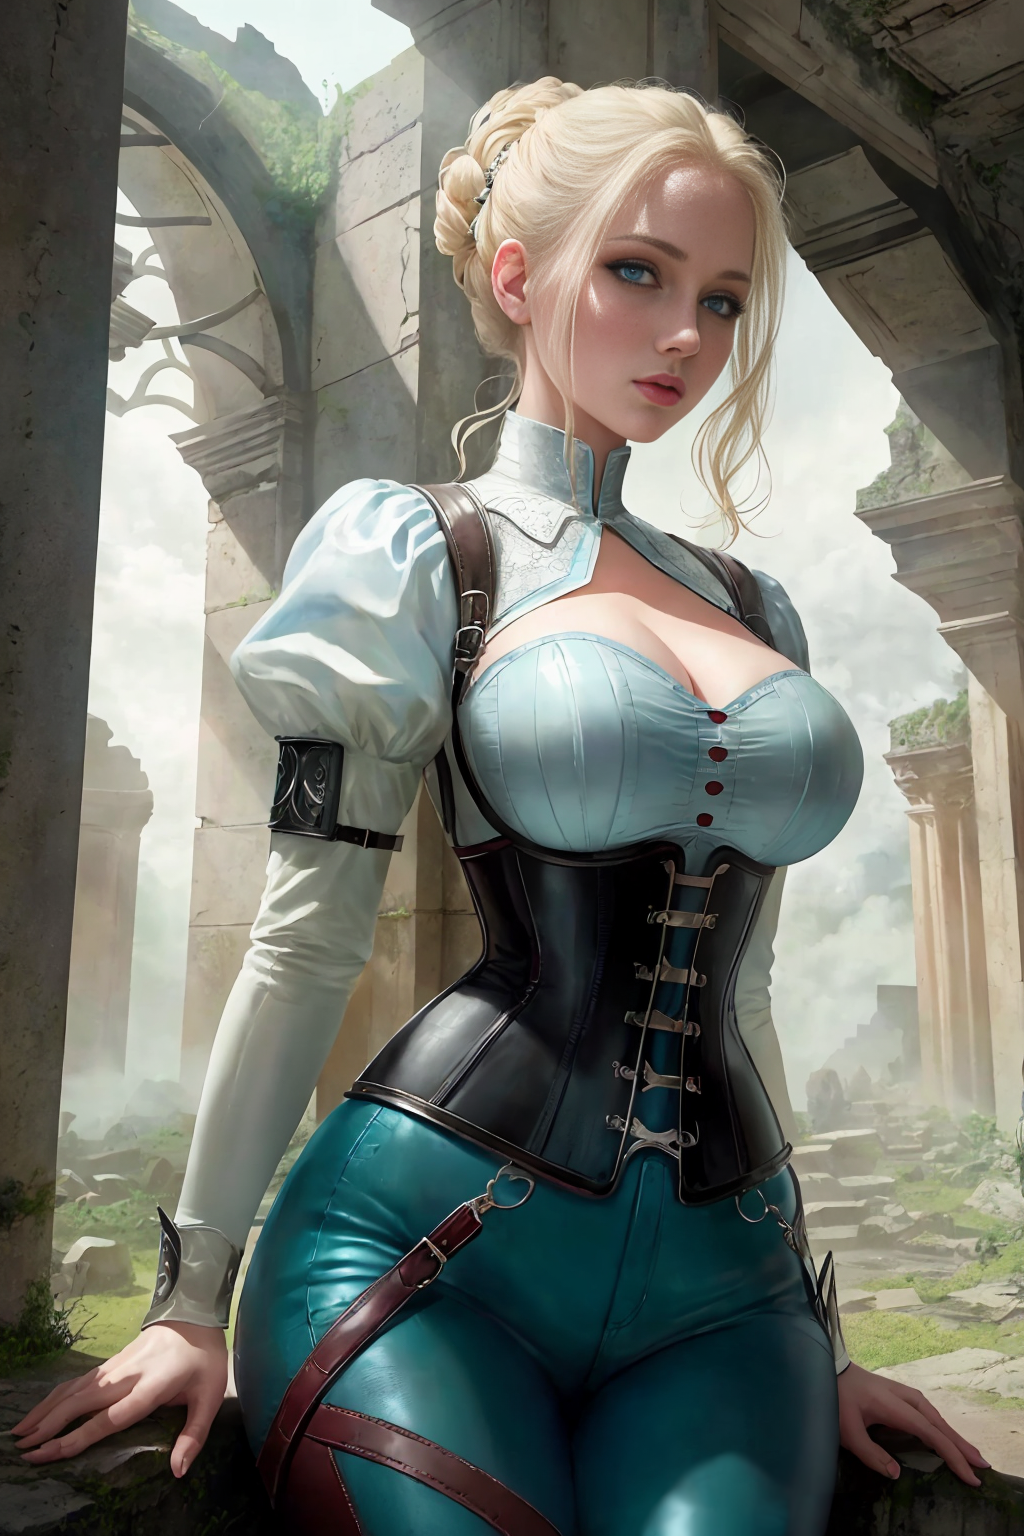
\includegraphics[scale=.37]{cover-image.png} %[scale=.45]
\vfill
\footnotesize{\textit{This material is Open Game Content, and is licensed for public use under the terms of the Open Game License v1.0a.}}\\
%\normalsize{\today}
\end{center}

\pagebreak

\sffamily
\pagestyle{plain}
\raggedbottom

%%%%%%%%%%%%%%%%%%%%%%%%%%%%%%%%%%%%%%%%%%%%%%%%%%
%%%%%%%%%%%%%%%%%%%%%%%%%%%%%%%%%%%%%%%%%%%%%%%%%%
%%% Table of Contents
%%%%%%%%%%%%%%%%%%%%%%%%%%%%%%%%%%%%%%%%%%%%%%%%%%
%%%%%%%%%%%%%%%%%%%%%%%%%%%%%%%%%%%%%%%%%%%%%%%%%%
\renewcommand{\contentsname}{Table of Contents}
\setcounter{tocdepth}{2}
\small{\tableofcontents}
%%%%%%%%%%%%%%%%%%%%%%%%%%%%%%%%%%%%%%%%%%%%%%%%%%
%%%%%%%%%%%%%%%%%%%%%%%%%%%%%%%%%%%%%%%%%%%%%%%%%%
%%% Main Content
%%%%%%%%%%%%%%%%%%%%%%%%%%%%%%%%%%%%%%%%%%%%%%%%%%
%%%%%%%%%%%%%%%%%%%%%%%%%%%%%%%%%%%%%%%%%%%%%%%%%%

%% Primary Chapters Here

\clearpage
%%%%%%%%%%%%%%%%%%%%%%%%%%%%%%%%%%%%%%%%%%%%%%%%%%
%%%%%%%%%%%%%%%%%%%%%%%%%%%%%%%%%%%%%%%%%%%%%%%%%%
\chapter{Basics}
%%%%%%%%%%%%%%%%%%%%%%%%%%%%%%%%%%%%%%%%%%%%%%%%%%
%%%%%%%%%%%%%%%%%%%%%%%%%%%%%%%%%%%%%%%%%%%%%%%%%%

\section{The Basics}

\subsection{The Core Mechanic}
Whenever you attempt an action that has some chance of failure, you roll a twenty-sided die (d20). To determine if your character succeeds at a task you do this:
\begin{itemize*}
	\item Roll a d20.
	\item Add any relevant modifiers.
	\item Compare the result to a target number.
\end{itemize*}

If the result equals or exceeds the target number, often called a Difficulty Class or DC, your character succeeds. If the result is lower than the target number, you fail.

\subsection{Dice}
Dice rolls are described with expressions such as ``3d4+3," which means ``roll three four-sided dice and add 3" (resulting in a number between 6 and 15). The first number tells you how many dice to roll (adding the results together). The number immediately after the ``d" tells you the type of die to use. Any number after that indicates a quantity that is added or subtracted from the result.

d\%: Percentile dice work a little differently. You generate a number between 1 and 100 by rolling two different ten-sided dice. One (designated before you roll) is the tens digit. The other is the ones digit. Two 0s represent 100.

\subsection{Rounding Fractions}
In general, if you wind up with a fraction, round down, even if the fraction is one-half or larger.
Exception: Certain rolls, such as damage and hit points, have a minimum of 1.

\subsection{Multiplying}
Sometimes a rule makes you multiply a number or a die roll. As long as you're applying a single multiplier, multiply the number normally. When two or more multipliers apply to any abstract value (such as a modifier or a die roll), however, combine them into a single multiple, with each extra multiple adding 1 less than its value to the first multiple. Thus, a double (2) and a double (2) applied to the same number results in a triple (3, because 2 + 1 = 3).

When applying multipliers to real-world values (such as weight or distance), normal rules of math apply instead. A creature whose size doubles (thus multiplying its weight by 8) and then is turned to stone (which would multiply its weight by a factor of roughly 3) now weighs about 24 times normal, not 10 times normal. Similarly, a blinded creature attempting to negotiate difficult terrain would count each square as 4 squares (doubling the cost twice, for a total multiplier of \^{x}4), rather than as 3 squares (adding 100\% twice). 

\section{Ability Scores}

\subsection{Ability Modifiers}

Each ability, after changes made because of race, has a modifier ranging from \textendash 5 to +5. Table: Ability Modifiers and Bonus Spells shows the modifier for each score. It also shows bonus spells, which you'll need to know about if your character is a spellcaster.
The modifier is the number you apply to the die roll when your character tries to do something related to
that ability. You also use the modifier with some numbers that aren't die rolls. A positive modifier is called a bonus, and a negative modifier is called a penalty.

\textbf{Abilities and Spellcasters:}{The ability that governs bonus spells depends on what type of spellcaster your character is: Intelligence for wizards; Wisdom for clerics, druids, paladins, and rangers; or Charisma for sorcerers and bards. In addition to having a high ability score, a spellcaster must be of high enough class level to be able to cast spells of a given spell level. (See the class descriptions for details.)}

\begin{spellperdaybasictable}
1        & -5    & \multicolumn{10}{c}{Can't cast spells tied to this ability}\\
2-3     & -4    & \multicolumn{10}{c}{Can't cast spells tied to this ability}\\
4-5     & -3    & \multicolumn{10}{c}{Can't cast spells tied to this ability}\\
6-7     & -2    & \multicolumn{10}{c}{Can't cast spells tied to this ability}\\
8-9     & -1    & \multicolumn{10}{c}{Can't cast spells tied to this ability}\\
10-11 & 0     & - & - & - & - & - & - & - & - & - & -\\
12-13 & +1   & 1 & - & - & - & - & - & - & - & - & -\\
14-15 & +2   & 1 & 1 & - & - & - & - & - & - & - & -\\
16-17 & +3   & 1 & 1 & 1 & - & - & - & - & - & - & -\\
18-19 & +4   & 1 & 1 & 1 & 1 & - & - & - & - & - & -\\
20-21 & +5   & 2 & 1 & 1 & 1 & 1 & - & - & - & - & -\\
22-23 & +6   & 2 & 2 & 1 & 1 & 1 & 1 & - & - & - & -\\
24-25 & +7   & 2 & 2 & 2 & 1 & 1 & 1 & 1 & - & - & -\\
26-27 & +8   & 2 & 2 & 2 & 2 & 1 & 1 & 1 & 1 & - & -\\
28-29 & +9   & 3 & 2 & 2 & 2 & 2 & 1 & 1 & 1 & 1 & -\\
30-31 & +10 & 3 & 3 & 2 & 2 & 2 & 2 & 1 & 1 & 1 & 1\\
32-33 & +11 & 3 & 3 & 3 & 2 & 2 & 2 & 2 & 1 & 1 & 1\\
34-35 & +12 & 3 & 3 & 3 & 3 & 2 & 2 & 2 & 2 & 1 & 1\\
36-37 & +13 & 4 & 3 & 3 & 3 & 3 & 2 & 2 & 2 & 2 & 1\\
38-39 & +14 & 4 & 4 & 3 & 3 & 3 & 3 & 2 & 2 & 2 & 2\\
\end{spellperdaybasictable}

\pagebreak

\subsection{The Abilities}
\vspace*{10pt}
Each ability partially describes your character and affects some of his or her actions.

\textbf{Altering an Ability Score:}
When an ability score changes, all attributes associated with that score change accordingly. A character does not retroactively get additional skill points for previous levels if she increases her intelligence.

\subsubsection{STRENGTH (STR)}

Strength measures your character's muscle and physical power. This ability is especially important for fighters, barbarians, paladins, rangers, and monks because it helps them prevail in combat. Strength also limits the amount of equipment your character can carry.
You apply your character's Strength modifier to:
\begin{itemize*}
	\item Melee attack rolls.
	\item Damage rolls when using a melee weapon or a thrown weapon (including a sling). (Exceptions: Off\textendash hand attacks receive only one\textendash half the character's Strength bonus, while two\textendash handed attacks receive one and a half times the Strength bonus. A Strength penalty, but not a bonus, applies to attacks made with a bow that is not a composite bow.)
	\item \linkskill{Climb}, \linkskill{Jump}, and \linkskill{Swim} checks. These are the skills that have Strength as their key ability.
	\item Strength checks (for breaking down doors and the like).
\end{itemize*}

\subsubsection{DEXTERITY (DEX)}

Dexterity measures hand\textendash eye coordination, agility, reflexes, and balance. This ability is the most important one for rogues, but it's also high on the list for characters who typically wear light or medium armor (rangers and barbarians) or no armor at all (monks, wizards, and sorcerers), and for anyone who wants to be a skilled archer.
You apply your character's Dexterity modifier to:
\begin{itemize*}
	\item Ranged attack rolls, including those for attacks made with bows, crossbows, throwing axes, and other ranged weapons.
	\item Armor Class (AC), provided that the character can react to the attack.
	\item Reflex saving throws, for avoiding fireballs and other attacks that you can escape by moving quickly.
	\item \linkskill{Balance}, \linkskill{Escape Artist}, \linkskill{Ride}, \linkskill{Sleight of Hand}, \linkskill{Hide}, \linkskill{Tumble}, and \linkskill{Use Rope} checks. These are the skills that have Dexterity as their key ability.
\end{itemize*}

\subsubsection{CONSTITUTION (CON)}

Constitution represents your character's health and stamina. A Constitution bonus increases a character's hit points, so the ability is important for all classes.
You apply your character's Constitution modifier to:
\begin{itemize*}
	\item Each roll of a Hit Die (though a penalty can never drop a result below 1\textendash that is, a character always gains at least 1 hit point each time he or she advances in level).
	\item Fortitude saving throws, for resisting poison and similar threats.
	\item \linkskill{Concentration} checks. \linkskill{Concentration} is a skill, important to spellcasters, that has Constitution as its key ability.
	\item If a character's Constitution score changes enough to alter his or her Constitution modifier, the character's hit points also increase or decrease accordingly.
\end{itemize*}

\subsubsection{INTELLIGENCE (INT)}

Intelligence determines how well your character learns and reasons. This ability is important for wizards because it affects how many spells they can cast, how hard their spells are to resist, and how powerful their spells can be. It's also important for any character who wants to have a wide assortment of skills.
You apply your character's Intelligence modifier to:
\begin{itemize*}
	\item The number of languages your character knows at the start of the game.
	\item The number of skill points gained each level. (But your character always gets at least 1 skill point per level.)
	\item \linkskill{Appraise}, \linkskill{Craft}, \linkskill{Decipher Script}, \linkskill{Disable Device}, \linkskill{Forgery}, \linkskill{Knowledge}, \linkskill{Search}, and \linkskill{Spellcraft} checks. These are the skills that have Intelligence as their key ability.
	\item Some classes cast spells based on Intelligence.  The minimum Intelligence score needed to cast a spell for such a class is 10 + the spell's level.
	\item An animal has an Intelligence score of 1 or 2. A creature of humanlike intelligence has a score of at least 3.
\end{itemize*}


\subsubsection{WISDOM (WIS)}

Wisdom describes a character's willpower, common sense, perception, and intuition. While Intelligence represents one's ability to analyze information, Wisdom represents being in tune with and aware of one's surroundings. Wisdom is the most important ability for clerics and druids, and it is also important for paladins and rangers. If you want your character to have acute senses, put a high score in Wisdom. Every creature has a Wisdom score.
You apply your character's Wisdom modifier to:
\begin{itemize*}
	\item Will saving throws (for negating the effect of charm person and other spells).
	\item \linkskill{Heal}, \linkskill{Profession}, \linkskill{Sense Motive}, and \linkskill{Survival} checks. These are the skills that have Wisdom as their key ability.
	\item Some classes cast spells based on Wisdom.  The minimum Wisdom score needed to cast a spell for such a class is 10 + the spell's level.
\end{itemize*}

\subsubsection{CHARISMA (CHA)}

Charisma measures a character's force of personality, persuasiveness, personal magnetism, ability to lead, and physical attractiveness. This ability represents actual strength of personality, not merely how one is perceived by others in a social setting. Charisma is most important for paladins, sorcerers, and bards. It is also important for clerics, since it affects their ability to turn undead. Every creature has a Charisma score.
You apply your character's Charisma modifier to:
\begin{itemize*}
	\item \linkskill{Bluff}, \linkskill{Diplomacy}, \linkskill{Disguise}, \linkskill{Gather Information}, \linkskill{Handle Animal}, \linkskill{Intimidate}, \linkskill{Perform}, and \linkskill{Use Magic Device} checks. These are the skills that have Charisma as their key ability.
	\item Checks that represent attempts to influence others.
	\item Some classes cast spells based on Charisma.  The minimum Charisma score needed to cast a spell for such a class is 10 + the spell's level.
\end{itemize*}

\vspace*{15pt}

%%%%%%%%%%%%%%%%%%%%%%%%%%%%%%%%%%%%%%%%%%%%%%%%%%
%%%%%%%%%%%%%%%%%%%%%%%%%%%%%%%%%%%%%%%%%%%%%%%%%%
\chapter{Character Creation}
%%%%%%%%%%%%%%%%%%%%%%%%%%%%%%%%%%%%%%%%%%%%%%%%%%
%%%%%%%%%%%%%%%%%%%%%%%%%%%%%%%%%%%%%%%%%%%%%%%%%%

%%%
\section{Character Creation}
%%%

To create a complete character there are several steps that you need to follow:

\begin{itemize}
\item Select Race (\hyperlink{chapter.3}{Chapter 3})
\item Select Class (\hyperlink{chapter.4}{Chapter 4})
\item Determine Ability Scores (\linksec{Generating Your Stats}{Below})
\item Assign Skill Points \hyperlink{chapter.5}{Chapter 5})
\item Select Feat (\hyperlink{chapter.6}{Chapter 6})
%\item Purchase Starting Equipment (\hyperlink{chapter.\#}{Chapter \#})
%\item Note Character Details (\hyperlink{chapter.\#}{Chapter \#})
\end{itemize}

\section{Generating Your Stats}

The first step of character creation is to generate the six ability scores that your character will have. There are two basic methods for doing this: Rolling and Point Buy. Check with your Game Master to see what method you should use to make your character.

\subsection{Rolling}

Rolling for your ability scores involves rolling a number of d6's and assigning the result to the desired ability.
\begin{itemize*}
	\item{3d6:} Roll 3d6 six time.
	\item{4d6 Drop Lowest:} Roll 4d6 and and drop the lowest dice six times.
	\item{4d6, Reroll Ones, Drop Lowest:} Roll 4d6, reroll any ones, and drop the lowest dice six times.
\end{itemize*}
\vspace*{10pt}
Once you've generated six totals you can assign them to the desired ability score.  Some GM's may use different numbers of dice to in order to generate ability scores.

\subsection{Point Buy}

\setlength{\intextsep}{-5pt}
\begin{wraptable}{O}{2in}
\caption{Point Buy Chart}
\rowcolors{1}{offyellow}{white}
\begin{tabular}{c|c c c|c}
Score & Cost & & Score & Cost \\
9  & 1       & & 14 & 6       \\
10 & 2       & & 15 & 8       \\
11 & 3       & & 16 & 10      \\
12 & 4       & & 17 & 13      \\
13 & 5       & & 18 & 16      \\
\multicolumn{4}{c}{\cellcolor{white}}{}\\
\multicolumn{4}{c}{\cellcolor{white}}{}\\
\multicolumn{4}{c}{\cellcolor{white}}{}\\
\end{tabular}
\end{wraptable}
\setlength{\intextsep}{10pt}

The other method for generating ability scores is to `buy' a certain score for each of your ability scores by `spending' a pool of points in order to determine your starting ability scores.  All racial modifiers are applied after you have bought scores for every attribute.  To use this method each of your scores starts out at 8, and you can buy a score with your points according to the the table. A `low\textendash power' campaign may use as few as 15 points, a `challenging' campaign 22 points, a `tough' campaign 28 points, and a `high\textendash powered' campaign may use 32 or more.  If the Game Master decides to use point buy, he ultimately decides how many points characters receive to buy their ability scores.

\section{Choose a Race}

The second step after generating and assigning your ability scores is to choose what race you want your character to be.  Your race determines your size, speed, type, and forms of vision.  Your race may also give you bonuses to certain ability scores, skills, grant you bonus feats, or give you many other sorts of bonuses and abilities.

\textbf{Languages: }Every Race has languages indicated as `Automatic' and `Bonus.'  Every character of a given race can speak and write in the listed Automatic Languages, for every point of Intelligence bonus that character posesses above +0 you may select one additional language from the list of Bonus Languages.

\hyperlink{chapter.3}{Chapter three} contains standard races to choose from. Though you may also choose races from the \linksec{Unusual Races} if GM allows.

\section{Choose an Alignment}

Alignment is a broad categorization that encompases your characters outlook on morality.  There are nine alignments derived from the axes of ``Law and Chaos" and of ``Good and Evil". Listed here are the default interpretations of alignment. Your GM or gaming group may have selected to treat ``Good and Evil" or ``Law and Chaos" in a way other than the defaults presented here, however, and the following may not apply (see the chapter on Alignment options for more information).
\vspace*{10pt}
\begin{itemize*}
	\item{Lawful Good:} A lawful good character acts as a good person is expected or required to act. She combines a commitment to oppose evil with the discipline to fight relentlessly. She tells the truth, keeps her word, helps those in need, and speaks out against injustice. A lawful good character hates to see the guilty go unpunished. 
	\item{Neutral Good:} A neutral good character does the best that a good person can do. He is devoted to helping others. He works with kings and magistrates but does not feel beholden to them.
	\item{Chaotic Good:} A chaotic good character acts as his conscience directs him with little regard for what others expect of him. He makes his own way, but he's kind and benevolent. He believes in goodness and right but has little use for laws and regulations. He hates it when people try to intimidate others and tell them what to do. He follows his own moral compass, which, although good, may not agree with that of society. 
	\item{Lawful Neutral:} A lawful neutral character acts as law, tradition, or a personal code directs her. Order and organization are paramount to her. She may believe in personal order and live by a code or standard, or she may believe in order for all and favor a strong, organized government. 
	\item{Neutral:} A neutral character does what seems to be a good idea. She doesn't feel strongly one way or the other when it comes to good vs. evil or law vs. chaos. Most neutral characters exhibit a lack of conviction or bias rather than a commitment to neutrality. Such a character thinks of good as better than evil after all, she would rather have good neighbors and rulers than evil ones. Still, she's not personally committed to upholding good in any abstract or universal way. Some neutral characters, on the other hand, commit themselves philosophically to neutrality. They see good, evil, law, and chaos as prejudices and dangerous extremes. They advocate the middle way of neutrality as the best, most balanced road in the long run. 
	\item{Chaotic Neutral:} A chaotic neutral character follows his whims. He is an individualist first and last. He values his own liberty but doesn't strive to protect others' freedom. He avoids authority, resents restrictions, and challenges traditions. A chaotic neutral character does not intentionally disrupt organizations as part of a campaign of anarchy. To do so, he would have to be motivated either by good (and a desire to liberate others) or evil (and a desire to make those different from himself suffer). A chaotic neutral character may be unpredictable, but his behavior is not totally random. He is not as likely to jump off a bridge as to cross it. 
	\item{Lawful Evil:}  A lawful evil villain methodically takes what he wants within the limits of his code of conduct without regard for whom it hurts. He cares about tradition, loyalty, and order but not about freedom, dignity, or life. He plays by the rules but without mercy or compassion. He is comfortable in a hierarchy and would like to rule, but is willing to serve. He condemns others not according to their actions but according to race, religion, homeland, or social rank. He is loath to break laws or promises. This reluctance comes partly from his nature and partly because he depends on order to protect himself from those who oppose him on moral grounds.
	\item{Neutral Evil:} A neutral evil villain does whatever she can get away with. She is out for herself, pure and simple. She sheds no tears for those she kills, whether for profit, sport, or convenience. She has no love of order and holds no illusion that following laws, traditions, or codes would make her any better or more noble. On the other hand, she doesn't have the restless nature or love of conflict that a chaotic evil villain has. 
	\item{Chaotic Evil:} A chaotic evil character does whatever his greed, hatred, and lust for destruction drive him to do. He is hot-tempered, vicious, arbitrarily violent, and unpredictable. If he is simply out for whatever he can get, he is ruthless and brutal. If he is committed to the spread of evil and chaos, he is even worse. Thankfully, his plans are haphazard, and any groups he joins or forms are poorly organized. Typically, chaotic evil people can be made to work together only by force, and their leader lasts only as long as he can thwart attempts to topple or assassinate him. 
\end{itemize*}
\vspace*{10pt}
Your character begins the game as the alignment of your choice, though the GM may decide that it changes through the course of play because of your actions.
 
\section{Choose a Class}

Your class is the primary method by which your character advances.  You start off with one level in a class of your choice.  Every time you gain a level in a class you gain all the features indicated in that classes table for that level.  This includes Base Attack Bonus, bonuses to your Saves, Hit Dice, Skill Points, and other class features.  Chapter 4 includes all the base classes you can take.

When you gain a new level you can take the next level of a class you already have levels in, or you can get the features from the first level of a new class.  The total of all the levels you have taken is your character level.

At first level you gain quadruple normal skill points for the class and get the maximum hit points possible for you classes hit die.

If you take one of your races favored classes at first level you get one of you races [Regional] Feat for free

At higher levels you may begin qualifying for prestige classes.  You gain levels in prestige classes the same way you do base classes with the exception that your character must meet the listed prerequisites for the class in order to begin taking levels.

\section{Skills}

Every class gives you a certain number of skill points that you can assign to skills.  Each point buys you one rank of a skill and every rank adds a +1 bonus to rolls involving the skill.  The maximum number points that you can invest in a class skill is your character level + 3, and the maximum ranks you can invest in a cross-class skill is half of your class skill maximum.

\section{Feats}

At first level, third level, and every third level thereafter your character gains a feat.  Feats represent abilities your character has but are not directly related to your class. Many, but not all, feats scale to one of your characters features. [Combat] feats scale to your base attack bonus, [Skill] feats scale to ranks in a specific skill, and [Magic] feats scale to the higest level spell you can cast, other types of feats may scale to other attributes.  [General] and [Metamagic] feats do not scale to any attribute.  Some feats have requirements that must be met in order to take them.

\section{Equipment}

Your character starts with a certain amount of gold that can be used to buy equipment that it will start with.  Later in the game you will gain access to powerful magic items and whatnot.


%%%%%%%%%%%%%%%%%%%%%%%%%%%%%%%%%%%%%%%%%%%%%%%%%%
%%%%%%%%%%%%%%%%%%%%%%%%%%%%%%%%%%%%%%%%%%%%%%%%%%
\chapter{Races}
%%%%%%%%%%%%%%%%%%%%%%%%%%%%%%%%%%%%%%%%%%%%%%%%%%
%%%%%%%%%%%%%%%%%%%%%%%%%%%%%%%%%%%%%%%%%%%%%%%%%%
\pagebreak
\section{Dwarf}
%%%%%%%%%%%%%%%%%%%%%%%%%%%%%%%%%%%%%%%%%%%%%%%%%%
\raceentry{Shield Dwarf}
%%%%%%%%%%%%%%%%%%%%%%%%%%%%%%%%%%%%%%%%%%%%%%%%%%

Found largely in the northern reaches of western and central Faerûn, Shield Dwarves are the dominant northern branch of the Stout Folk. Renowned for their smithwork and craftsmanship, Shield Dwarves have endured a centuries-long decline in the face of never-ending wars with orcs, goblins, giants, and trolls. Shield dwarves are descended from the founders of Shanatar, a legendary dwarven empire that once ruled the caverns beneath modern-day Amn, Tethyr, and Calimshan. After Shanatar fell, the Shield Dwarves migrated north, founding kingdoms such as Ammarindar, Delzoun, Gharraghaur, Haunghdannar, Oghrann, and Sarbreen. Although those kingdoms have also largely fallen, the Stout Folk of the North endure. The Thunder Blessing has served as a welcome reprieve for the beleaguered Shield Dwarves, giving hope that the descendants of ancient Shanatar may one day reclaim the glory of their forebears. Taller by half a foot than their Gold Dwarf cousins, Shield dwarves average 4 1/2 feet tall and weigh as much as an adult human. The skin of a Shield Dwarf is fair or lightly tanned, and her eyes are usually green or silvered blue. Both genders wear their hair long, and males (and a very few females) have long, carefully groomed beards and mustaches. Hair color ranges from light brown to red, with all shades fading to silver or white as time progresses. Shield dwarves keep to their word, whatever the cost, and are incredibly stubborn, unwilling to concede an inch unless there is absolutely no alternative. Such intransigence has enabled dwindling Shield Dwarf populations to hold on to ancient strongholds with just a fraction of their original defenders. However, it has also led to clan feuds and long-standing misunderstandings with other races that have sapped the strength of the Stout Folk. Shield dwarves love worked beauty, seeing the world as raw material to be forged and shaped into something more than the original

\begin{multicols}{2}

\begin{itemize*}
\item Medium size.
\item Dwarf base land speed is 20 feet. However, Shield Dwarves doesn't have their movement speed reduced from armour.
\item Humanoid Type (Dwarf subtype)
\item \linkability{Darkvision} 60ft
\item +2 Constitution, -2 Charisma.
\item Stonecunning: This ability grants the dwarf a +2 racial bonus on \linkskill{Search} checks to notice unusual stonework, such as sliding walls, stonework traps, new construction (even when built to match the old), unsafe stone surfaces, shaky stone ceilings, and the like. Something that isn't stone but that is disguised as stone also counts as unusual stonework. A Shield Dwarf who merely comes within 10 feet of unusual stonework can make a \linkskill{Search} check as if he were actively searching, and can use the \linkskill{Search} skill to find stonework traps; they can also intuit depth, sensing his approximate depth underground as naturally as a human can sense which way is up.
\item Weapon Familiarity: Shield Dwarves may treat dwarven waraxes and dwarven urgroshes as martial weapons, rather than exotic weapons.
\item Stability: Shield Dwarf gains a +4 bonus on ability checks made to resist being bull rushed or tripped when standing on the ground (but not when climbing, flying, riding, or otherwise not standing firmly on the ground).
\item +2 racial bonus on saving throws against poison.
\item +2 racial bonus on saving throws against spells and spell-like effects.
\item +1 racial bonus on attack rolls against orcs and goblinoids.
\item +4 dodge bonus to Armor Class against monsters of the giant type.
\item +2 racial bonus on \linkskill{Appraise} checks that are related to stone or metal items.
\item +2 racial bonus on \linkskill{Craft} checks that are related to stone or metal.
\item Alignment: Often lawful good
\item Favored Classes: \linkclass{Barbarian} and \linkclass{Fighter}
\end{itemize*}

\begin{multicolsbasictable}{c*{4}{c}}

\textbf{Adulthood} & \textbf{Simple} & \textbf{Moderate} & \textbf{Complex}\\
40 & +3d6 & +5d6 & +7d6\\
\multicolumn{2}{c}{\textbf{Base Height}} & \multicolumn{2}{c}{\textbf{Base Height}}\\
\textbf{Male} &\textbf{Female} & \multicolumn{2}{c}{\textbf{Modifier}}\\
4'2'' & 4'0'' & \multicolumn{2}{c}{+2d4}\\
\multicolumn{2}{c}{\cellcolor{white}\textbf{Base Weight}} & \multicolumn{2}{c}{\cellcolor{white}\textbf{Base Weight}}\\
\cellcolor{offyellow}\textbf{Male} & \cellcolor{offyellow}\textbf{Female} & \multicolumn{2}{c}{\cellcolor{offyellow}\textbf{Modifier}}\\
\cellcolor{white} 145 lb. & \cellcolor{white}110 lb. & \multicolumn{2}{c}{\cellcolor{white}X (2d6) lb.}\\
\end{multicolsbasictable}

\end{multicols}

\pagebreak

\begin{smallbasictable}{Shield Dwarf Regions}{l l p{4cm} p{3cm}}
\textbf{Region} & \textbf{Automatic Laguages} & \textbf{Bonus Languages} & \textbf{[Regional] Feat}\\
 The Galena Mountains & Damaran, Dwarven & \multicolumn{1}{p{4cm}}{\raggedright{}Chondathan, Giant, Goblin, Orc} & \multicolumn{1}{p{3cm}}{\raggedright{}\linkfeat{Dauntless}, \linkfeat{Foe Hunter} (Goblin), \linkfeat{Tireless}}\\
 The Great Glacier & Dwarven, Uluik & \multicolumn{1}{p{4cm}}{\raggedright{}Aquan, Auran, Damaran, Draconic, Giant} & \multicolumn{1}{p{3cm}}{\raggedright{}\linkfeat{Axethrower}, \linkfeat{Oral History}, \linkfeat{Survivor}}\\
 The Spine of the World & Dwarven & \multicolumn{1}{p{4cm}}{\raggedright{}Chondathan, Draconic, Giant, Goblin, Illuskan, Orc} & \multicolumn{1}{p{3cm}}{\raggedright{}\linkfeat{Bullheaded}, \linkfeat{Foe Hunter} (Orc), \linkfeat{Oral History}}\\
 The Sword Coast & Dwarven, Illuskan & \multicolumn{1}{p{4cm}}{\raggedright{}Chondathan, Elven, Giant, Gnome, Orc} & \multicolumn{1}{p{3cm}}{\raggedright{}\linkfeat{Forgeheart}, \linkfeat{Metallurgy}, \linkfeat{Tireless}}\\
 Turmish & Dwarven, Turmic & \multicolumn{1}{p{4cm}}{\raggedright{}Chondathan, Elven, Giant, Gnome, Halfling} & \multicolumn{1}{p{3cm}}{\raggedright{}\linkfeat{Dauntless}, \linkfeat{Silver Palm}, \linkfeat{Stoneshaper}}\\
 Underdark (Earthroot) & Dwarven & \multicolumn{1}{p{4cm}}{\raggedright{}Elven, Giant, Goblin, Orc, Terran} & \multicolumn{1}{p{3cm}}{\raggedright{}\linkfeat{Blooded}, \linkfeat{Bullheaded}, \linkfeat{Dauntless}}\\
 Underdark (Old Shanatar) & Dwarven & \multicolumn{1}{p{4cm}}{\raggedright{}Aquan, Draconic, Elven, Gnome, Terran} & \multicolumn{1}{p{3cm}}{\raggedright{}\linkfeat{Azerblood}, \linkfeat{Batrider}, \linkfeat{Tireless}}\\
 Waterdeep & Dwarven & \multicolumn{1}{p{4cm}}{\raggedright{}Alzhedo, Chondathan, Elven, Halfling, Illuskan, Orc} & \multicolumn{1}{p{3cm}}{\raggedright{}\linkfeat{Cosmopolitan}, \linkfeat{Silver Palm}, \linkfeat{Thug}}\\
\end{smallbasictable}

\pagebreak
\pagebreak
%%%%%%%%%%%%%%%%%%%%%%%%%%%%%%%%%%%%%%%%%%%%%%%%%%
\raceentry{Urdunnir}
%%%%%%%%%%%%%%%%%%%%%%%%%%%%%%%%%%%%%%%%%%%%%%%%%%

Urdunnirs, sometimes known as orecutter dwarves, are a longforgotten offshoot of shield dwarves who have become one with the earth and stone. Thanks to the blessings of Dumathoin, Urdunnirs can walk through earth and stone as if it were air and shape metal and stone with their hands. Many orecutter dwarves are clerics of Dumathoin, expert smiths, or expert gemcutters. The Children of Dumathoin, as they call themselves, believe that the Silent Keeper transformed their ancestors in order to create a race of dwarves who could appreciate the true beauty of the subterranean landscape without needing to destroy it in the process. They have dwelt ever since in splendid isolation in Oldonnar, the legendary Lost Kingdom of Shanatar, deep beneath the Alimir Mountains.

\begin{multicols}{2}

\begin{itemize*}
\item Medium size.
\item Dwarf base land speed is 20 feet. However, Urdunnirs doesn't have their movement speed reduced from armour.
\item Humanoid Type (Dwarf subtype)
\item \linkability{Darkvision} 60ft
\item +2 Constitution, -2 Charisma.
\item Stonecunning: This ability grants the dwarf a +2 racial bonus on \linkskill{Search} checks to notice unusual stonework, such as sliding walls, stonework traps, new construction (even when built to match the old), unsafe stone surfaces, shaky stone ceilings, and the like. Something that isn't stone but that is disguised as stone also counts as unusual stonework. A Urdunnir who merely comes within 10 feet of unusual stonework can make a \linkskill{Search} check as if he were actively searching, and can use the \linkskill{Search} skill to find stonework traps; they can also intuit depth, sensing his approximate depth underground as naturally as a human can sense which way is up.
\item Weapon Familiarity: Urdunnirs may treat dwarven waraxes and dwarven urgroshes as martial weapons, rather than exotic weapons.
\item Stability: Urdunnir gains a +4 bonus on ability checks made to resist being bull rushed or tripped when standing on the ground (but not when climbing, flying, riding, or otherwise not standing firmly on the ground).
\item +4 racial bonus on saving throws against poison.
\item +2 racial bonus on saving throws against spells and spell-like effects.
\item +1 racial bonus on attack rolls against orcs and goblinoids.
\item +4 dodge bonus to Armor Class against monsters of the giant type.
\item +2 racial bonus on \linkskill{Appraise} checks that are related to stone or metal items.
\item +2 racial bonus on \linkskill{Craft} checks that are related to stone or metal.
\item Light Blindness (Ex): Abrupt exposure to bright light (such as sunlight or a daylight spell) blinds aUrdunnir for 1 round. In addition, he takes a –1 circumstance penalty on all attack rolls, saves, and checks while operating in bright light.
\item Alignment: Usually Neutral
\item Favored Classes: \linkclass{Cleric} and \linkclass{Fighter}
\end{itemize*}

\begin{multicolsbasictable}{c*{4}{c}}

\textbf{Adulthood} & \textbf{Simple} & \textbf{Moderate} & \textbf{Complex}\\
40 & +3d6 & +5d6 & +7d6\\
\multicolumn{2}{c}{\textbf{Base Height}} & \multicolumn{2}{c}{\textbf{Base Height}}\\
\textbf{Male} &\textbf{Female} & \multicolumn{2}{c}{\textbf{Modifier}}\\
4'2'' & 4'0'' & \multicolumn{2}{c}{+2d4}\\
\multicolumn{2}{c}{\cellcolor{white}\textbf{Base Weight}} & \multicolumn{2}{c}{\cellcolor{white}\textbf{Base Weight}}\\
\cellcolor{offyellow}\textbf{Male} & \cellcolor{offyellow}\textbf{Female} & \multicolumn{2}{c}{\cellcolor{offyellow}\textbf{Modifier}}\\
\cellcolor{white} 180 lb. & \cellcolor{white}150 lb. & \multicolumn{2}{c}{\cellcolor{white}X (2d8) lb.}\\
\end{multicolsbasictable}

\end{multicols}

\pagebreak
Urdunnir Dwarf
\begin{smallbasictable}{Urdunnir Regions}{l l p{4cm} p{3cm}}
\textbf{Region} & \textbf{Automatic Laguages} & \textbf{Bonus Languages} & \textbf{[Regional] Feat}\\
The Galena Mountains & Damaran, Dwarven & \multicolumn{1}{p{4cm}}{\raggedright{}Chondathan, Giant, Goblin, Orc} & \multicolumn{1}{p{3cm}}{\raggedright{}\linkfeat{Dauntless}, \linkfeat{Foe Hunter} (Goblin), \linkfeat{Tireless}}\\
The Great Glacier & Dwarven, Uluik & \multicolumn{1}{p{4cm}}{\raggedright{}Aquan, Auran, Damaran, Draconic, Giant} & \multicolumn{1}{p{3cm}}{\raggedright{}\linkfeat{Axethrower}, \linkfeat{Oral History}, \linkfeat{Survivor}}\\
The Spine of the World & Dwarven & \multicolumn{1}{p{4cm}}{\raggedright{}Chondathan, Draconic, Giant, Goblin, Illuskan, Orc} & \multicolumn{1}{p{3cm}}{\raggedright{}\linkfeat{Bullheaded}, \linkfeat{Foe Hunter} (Orc), \linkfeat{Oral History}}\\
The Sword Coast & Dwarven, Illuskan & \multicolumn{1}{p{4cm}}{\raggedright{}Chondathan, Elven, Giant, Gnome, Orc} & \multicolumn{1}{p{3cm}}{\raggedright{}\linkfeat{Forgeheart}, \linkfeat{Metallurgy}, \linkfeat{Tireless}}\\
Turmish & Dwarven, Turmic & \multicolumn{1}{p{4cm}}{\raggedright{}Chondathan, Elven, Giant, Gnome, Halfling} & \multicolumn{1}{p{3cm}}{\raggedright{}\linkfeat{Dauntless}, \linkfeat{Silver Palm}, \linkfeat{Stoneshaper}}\\
Underdark (Earthroot) & Dwarven & \multicolumn{1}{p{4cm}}{\raggedright{}Elven, Giant, Goblin, Orc, Terran} & \multicolumn{1}{p{3cm}}{\raggedright{}\linkfeat{Blooded}, \linkfeat{Bullheaded}, \linkfeat{Dauntless}}\\
Underdark (Old Shanatar) & Dwarven & \multicolumn{1}{p{4cm}}{\raggedright{}Aquan, Draconic, Elven, Gnome, Terran} & \multicolumn{1}{p{3cm}}{\raggedright{}\linkfeat{Azerblood}, \linkfeat{Batrider}, \linkfeat{Tireless}}\\
Waterdeep & Dwarven & \multicolumn{1}{p{4cm}}{\raggedright{}Alzhedo, Chondathan, Elven, Halfling, Illuskan, Orc} & \multicolumn{1}{p{3cm}}{\raggedright{}\linkfeat{Cosmopolitan}, \linkfeat{Silver Palm}, \linkfeat{Thug}}\\
Oldonnar & Dwarven & \multicolumn{1}{p{4cm}}{\raggedright{}Draconic, Elven, Giant, Terran} & \multicolumn{1}{p{3cm}}{\raggedright{}\linkfeat{Magic in the Blood}, \linkfeat{Stoneshape}, \linkfeat{Strong Soul}}\\
Tethyr & Dwarven & \multicolumn{1}{p{4cm}}{\raggedright{}Alzhedo, Chondathan, Elven, Goblin, Orc} & \multicolumn{1}{p{3cm}}{\raggedright{}\linkfeat{Blooded}, \linkfeat{Furious Charge}, \linkfeat{Luck of Heroes}}\\
The Lake of Steam & Dwarven & \multicolumn{1}{p{4cm}}{\raggedright{}Alzhedo, Chondathan, Goblin, Shaaran, Tashalan} & \multicolumn{1}{p{3cm}}{\raggedright{}\linkfeat{Knifefighter}, \linkfeat{Snake Blood}, \linkfeat{Stormheart}}\\
The North & Dwarven & \multicolumn{1}{p{4cm}}{\raggedright{}Chondathan, Elven, Giant, Goblin, Illuskan Orc,} & \multicolumn{1}{p{3cm}}{\raggedright{}\linkfeat{Axethrower}, \linkfeat{Foe Hunter} (Orc), \linkfeat{Jotunbrud}}\\
\end{smallbasictable}

\pagebreak
\pagebreak
\section{Elf}
%%%%%%%%%%%%%%%%%%%%%%%%%%%%%%%%%%%%%%%%%%%%%%%%%%
\raceentry{Aquatic Elf}
%%%%%%%%%%%%%%%%%%%%%%%%%%%%%%%%%%%%%%%%%%%%%%%%%%

Rarely encountered by the landbound races, the aquatic elves are a civilized and good-hearted people who inhabit the seas surrounding Faerûn. Most aquatic elves hail from underwater cities in the Sea of Fallen Stars or in the Great Sea south of Faerûn, but small settlements of this race can be found in the seas along Faerûn’s western coasts as well.

The aquatic elves are tall, standing 6 feet or more in height. They have long limbs with strong swimming muscles, and their fingers and toes are long with thick webbing. Their most striking features are sets of gills along the collarbone and ribcage. Aquatic elves are nowhere near as thin as their landbound cousins, and their hair is usually stringy and thick, cut short for warriors but otherwise worn long. Great Sea aquatic elves have radiant skin of deep green with irregular thin brown stripes and patches. Aquatic elves from the Sea of Fallen Stars have skin in many shades of blue with white patches and stripes. Eye colors for both types of aquatic elf come in every shade seen among gold, moon, or wild elves. Their clothing is made of various undersea plants in shades of green, black, and brown, although aquatic elves usually go about lightly clad, if dressed at all, while underwater.

\begin{multicols}{2}

\begin{itemize*}
\item Medium sized.
\item 30ft movement, 40ft swin movement
\item Humanoid Type (Elf subtype)
\item \linkability{Low-Light Vision} (Ex)
\item Gills (Ex): Aquatic elves breathe salt water with ease. They can also breathe fresh water, but most find the experience to be very uncomfortable and are treated as fatigued while doing so and for 10 minutes afterward. Aquatic elves can survive out of the water for 1 hour per point of Constitution.
\item +2 Dexterity, -2 Intelligence.
\item Weapon Proficiency: The Aquatic Elves start proficient with trident, longspear, and net.
\item +8 racial bonus on all \linkskill{Swim} checks and can always choose to take 10 with \linkskill{Swim} checks, even if rushed or threatened. Aquatic elves can use the run action while swimming, as long as they swim in a straight line.
\item Alignment: Usually chaotic good
\item Favored Classes: \linkclass{Fighter} and \linkclass{Ranger}
\end{itemize*}

\begin{multicolsbasictable}{c*{4}{c}}

\textbf{Adulthood} & \textbf{Simple} & \textbf{Moderate} & \textbf{Complex}\\
110 & +4d6 & +6d6 & +10d6\\
\multicolumn{2}{c}{\textbf{Base Height}} & \multicolumn{2}{c}{\textbf{Base Height}}\\
\textbf{Male} &\textbf{Female} & \multicolumn{2}{c}{\textbf{Modifier}}\\
4'10'' & 4'5'' & \multicolumn{2}{c}{+2d10}\\
\multicolumn{2}{c}{\cellcolor{white}\textbf{Base Weight}} & \multicolumn{2}{c}{\cellcolor{white}\textbf{Base Weight}}\\
\cellcolor{offyellow}\textbf{Male} & \cellcolor{offyellow}\textbf{Female} & \multicolumn{2}{c}{\cellcolor{offyellow}\textbf{Modifier}}\\
\cellcolor{white} 90 lb. & \cellcolor{white}70 lb. & \multicolumn{2}{c}{\cellcolor{white}X (2d4) lb.}\\
\end{multicolsbasictable}

\end{multicols}

\begin{smallbasictable}{Aquatic Elf Regions}{c*{4}{c}}
\textbf{Region} & \multicolumn{1}{p{2cm}}{\raggedright{}\textbf{Automatic Laguages}} & \multicolumn{1}{p{5cm}}{\raggedright{}\textbf{Bonus Languages}} & \multicolumn{1}{p{5cm}}{\raggedright{}\textbf{[Regional] Feat}}\\
 The Inner Sea & Elven, Serusan & \multicolumn{1}{p{5cm}}{\raggedright{}Aquan, Chondathan, Draconic, Giant, Sylvan} & \multicolumn{1}{p{5cm}}{\raggedright{}\linkfeat{Blooded}, \linkfeat{Landwalker}, \linkfeat{Survivor}}\\
The Outer Sea & Elven, Serusan & \multicolumn{1}{p{5cm}}{\raggedright{}Alzhedo, Chondathan, Draconic, Illuskan} & \multicolumn{1}{p{5cm}}{\raggedright{}\linkfeat{Blooded}, \linkfeat{Survivor}, \linkfeat{Swift and Silent}}\\
\end{smallbasictable}

\pagebreak
\pagebreak
%%%%%%%%%%%%%%%%%%%%%%%%%%%%%%%%%%%%%%%%%%%%%%%%%%
\raceentry{Avariel}
%%%%%%%%%%%%%%%%%%%%%%%%%%%%%%%%%%%%%%%%%%%%%%%%%%

The avariels, or winged elves, are without a doubt the most reclusive and least numerous of the elven subraces on Faerûn. Many scholars have long dismissed them as creatures of myth. In truth, small numbers of avariels still dwell in Faerûn, concealed in hidden enclaves and remote regions.

The most striking feature of the avariels is their soft, feathered wings. These wings have spans of anywhere from twelve to sixteen feet and are usually white, but may also be gray, brown, black, or speckled. Avariels take great pride in their wings and spend long hours grooming them. Their skin is pale, often porcelain white, with tinges of blue or faint silver. They have silverwhite or black hair, with other shades being rare but not unheard of. The avariels’ eyes are rather large and more expressive than those of other elves, and they tend to be brilliant shades of blue or green. A few avariel have scintillating violet eyes as pure as amethysts. Avariels stand 5'9" tall on average, with thin, graceful limbs and angular facial features. They are the most beautiful and striking of the elven races, although too often this beauty is marred by haughtiness and condescension toward their landbound kin, whom they often pity.

Avariels are even more delicate than other elves, and their movements are quick, calculated, and graceful. They prefer to wear loose fitting, diaphanous clothing that catches the wind in flight and ripples and weaves in the air. Armor is almost never worn, because it tends to weigh the avariels down and hinder their graceful motion. Avariels cannot fly while wearing heavy armor.
\begin{multicols}{2}

\begin{itemize*}
\item Medium sized.
\item 30ft movement, 50ft fly movement
\item Humanoid Type (Elf subtype)
\item Keen Sight (Ex): Avariels gain a +4 racial bonus on all \linkskill{Spot} checks.
\item Flight (Ex): Avariels have a flying speed of 50 feet with average maneuverability, as long as they do not carry more than a Medium load, are not wearing Heavy armor, and are not fatigued or exhausted. Avariel wings have a span of 12 feet on average; they cannot fly in an area that does not allow them to fully extend their wings.

An avariel may make a dive attack. A dive attack works just like a charge, but the avariel must descend a minimum of 30 feet and attack with a piercing weapon; if she hits, she deals double damage. An avariel can use the run action while flying, provided she flies in a straight line.
\item +4 Dexterity, –2 Constitution, +2 Intelligence, +2 Wisdom. Avariels have hollow bones and, as a result, are more fragile than humans. At the same time, they are gifted with a keen intuition and intellect, and an almost otherworldly grace
\item Weapon Proficiency: The Avariel start proficient with rapier, longsword, lasso and bolas.
\item +4 racial bonus on \linkskill{Jump} checks. They are strong for their weight.
\item Alignment: Usually chaotic good
\item Favored Classes: \linkclass{Cleric} and \linkclass{Ranger}
\end{itemize*}

\begin{multicolsbasictable}{c*{4}{c}}

\textbf{Adulthood} & \textbf{Simple} & \textbf{Moderate} & \textbf{Complex}\\
110 & +4d6 & +6d6 & +10d6\\
\multicolumn{2}{c}{\textbf{Base Height}} & \multicolumn{2}{c}{\textbf{Base Height}}\\
\textbf{Male} &\textbf{Female} & \multicolumn{2}{c}{\textbf{Modifier}}\\
5'0" & 4'8" & \multicolumn{2}{c}{+2d8}\\
\multicolumn{2}{c}{\cellcolor{white}\textbf{Base Weight}} & \multicolumn{2}{c}{\cellcolor{white}\textbf{Base Weight}}\\
\cellcolor{offyellow}\textbf{Male} & \cellcolor{offyellow}\textbf{Female} & \multicolumn{2}{c}{\cellcolor{offyellow}\textbf{Modifier}}\\
\cellcolor{white} 70 lb. & \cellcolor{white}65 lb. & \multicolumn{2}{c}{\cellcolor{white}X (1d6) lb.}\\
\end{multicolsbasictable}

\end{multicols}

\begin{smallbasictable}{Avariel Regions}{c*{4}{c}}
\textbf{Region} & \multicolumn{1}{p{2cm}}{\raggedright{}\textbf{Automatic Laguages}} & \multicolumn{1}{p{5cm}}{\raggedright{}\textbf{Bonus Languages}} & \multicolumn{1}{p{5cm}}{\raggedright{}\textbf{[Regional] Feat}}\\
Snow Eagle Aerie & Auran, Elven & \multicolumn{1}{p{5cm}}{\raggedright{}Damaran, Draconic, Giant, Rashemi, Sylvan, Tuigan} & \multicolumn{1}{p{5cm}}{\raggedright{}\linkfeat{Artist}, \linkfeat{Mind over Body}, \linkfeat{Rapid Flight}}\\
\end{smallbasictable}

\pagebreak
\pagebreak
%%%%%%%%%%%%%%%%%%%%%%%%%%%%%%%%%%%%%%%%%%%%%%%%%%
\raceentry{Drow}
%%%%%%%%%%%%%%%%%%%%%%%%%%%%%%%%%%%%%%%%%%%%%%%%%%

Of the various elven subraces, none are more notorious than the Drow. Descended from the original dark-skinned Elven subrace called the Ssri-tel-quessir, the Drow were cursed into their present appearance by the good Elven deities for following the goddess Lolth down the path to evil and corruption. Also called Dark Elves, the Drow have black skin that resembles polished obsidian and stark white or pale yellow hair. They commonly have blood-red eyes, although pale eyes (so pale as to be often mistaken for white) in shades of pale lilac, silver, pink, and blue are not unknown. They also tend to be smaller and thinner than most Faerûnian Elves. Most Drow on the surface are evil and worship Vhaeraun, but some outcasts and renegades have a more neutral attitude, and there are even groups of good Drow who worship Eilistraee or other deities not of the traditional Drow pantheon.

Though divided by endless feuds and schisms, the Drow are united in one terrible desire: they seethe with a hatred for the surface Elves. By their way of reckoning, they proved themselves the superior race in the Fourth Crown War, and the fact that the Seldarine (and Corellon in particular) punished them for their success is a poison that churns in their hearts and minds eternally. They burn with hatred for the Seldarine and their coddled children, and want nothing more than to return to the surface and bring to the elves there suffering a thousand times greater than that which the drow have been forced to endure over the past ten thousand years.

\begin{multicols}{2}

\begin{itemize*}
\item Medium Size
\item 30ft movement.
\item Humanoid Type (Elf subtype)
\item \linkability{Darkvision} 60ft
\item +2 Dexterity, –2 Constitution. The drow have ruthlessly selected for agility, intelligence, and force of personality over generations.
\item Daylight Sensitivity: While in brightly lit surroundings (such as a \linkspell{daylight} spell), a Drow suffers a -2 penalty to attack rolls and precision-based skill checks.
\item +2 bonus to saving throws against spells and spell-like abilities.
\item +2 bonus to \linkskill{Spot}, and \linkskill{Listen} checks. A Drow who merely passes within 5 feet of a secret or concealed door is entitled to a Search check to notice it as if she were actively looking for it. A Drow’s senses are so keen that she practically has a sixth sense about hidden portals.
\item Drow never sleep and are immune to \linkcondition{sleep} effects. Drow must still perform their 4 hour daily trance to stay coherent and rested.
\item Proficient with either rapier, shortsword, hand crossbow and light crossbow
\item Alignment: Usually evil
\item Favored Classes: \linkclass{Cleric} and \linkclass{Wizard}
\end{itemize*}

\begin{multicolsbasictable}{c*{4}{c}}

\textbf{Adulthood} & \textbf{Simple} & \textbf{Moderate} & \textbf{Complex}\\
110 & +4d6 & +6d6 & +10d6\\
\multicolumn{2}{c}{\textbf{Base Height}} & \multicolumn{2}{c}{\textbf{Base Height}}\\
\textbf{Male} &\textbf{Female} & \multicolumn{2}{c}{\textbf{Modifier}}\\
4'5'' & 4'5'' & \multicolumn{2}{c}{+2d6}\\
\multicolumn{2}{c}{\cellcolor{white}\textbf{Base Weight}} & \multicolumn{2}{c}{\cellcolor{white}\textbf{Base Weight}}\\
\cellcolor{offyellow}\textbf{Male} & \cellcolor{offyellow}\textbf{Female} & \multicolumn{2}{c}{\cellcolor{offyellow}\textbf{Modifier}}\\
\cellcolor{white} 85 lb. & \cellcolor{white} 80 lb. & \multicolumn{2}{c}{\cellcolor{white} X (1d6) lb.}\\
\end{multicolsbasictable}

\end{multicols}

\begin{smallbasictable}{Drow Regions}{c*{4}{c}}
\textbf{Region} & \multicolumn{1}{p{2cm}}{\raggedright{}\textbf{Automatic Laguages}} & \multicolumn{1}{p{5cm}}{\raggedright{}\textbf{Bonus Languages}} & \multicolumn{1}{p{5cm}}{\raggedright{}\textbf{[Regional] Feat}}\\
Cormanthor Drow & Elven & \multicolumn{1}{p{5cm}}{\raggedright{}Abyssal, Chondathan, Draconic, Drow Sign, Orc, Sylvan} & \multicolumn{1}{p{5cm}}{\raggedright{}\linkfeat{Blooded}, \linkfeat{Daylight Adaptation}, \linkfeat{Swift and Silent}}\\
Menzoberranyr & Elven & \multicolumn{1}{p{5cm}}{\raggedright{}Abyssal, Draconic, Drow Sign, Goblin, Illuskan} & \multicolumn{1}{p{5cm}}{\raggedright{}\linkfeat{Arachnid Rider}, \linkfeat{Magic in the Blood}, \linkfeat{Twin Sword Style}}\\
\end{smallbasictable}

\pagebreak
\pagebreak
%%%%%%%%%%%%%%%%%%%%%%%%%%%%%%%%%%%%%%%%%%%%%%%%%%
\raceentry{Moon Elf}
%%%%%%%%%%%%%%%%%%%%%%%%%%%%%%%%%%%%%%%%%%%%%%%%%%

The most common of the elven subraces on Faerûn are the Moon Elves. They have fair skin, sometimes tinged with blue, and hair of silver-white, black, or blue; humanlike colors are somewhat rare. Their eyes are blue or green, with gold flecks. Moon Elves prefer to dress in rustic clothes of simple cuts and fashions that are nevertheless of fine and exquisite make. They adorn their dress with embroidered patterns, beads, and similar trappings, preferring earthen colors for everyday wear, hues that make it easy to conceal themselves in foliage. In places of safety or in times of revelry, Moon Elves enjoy dressing in bold colors— the more brightly colored, the better. Hair is worn in braids or ponytails, twined with wires or beads. Moon Elves sometimes wear body paint or tattoos in mystic patterns, although not to extent the wild elves do.

\begin{multicols}{2}

\begin{itemize*}
\item Medium sized.
\item 30ft movement
\item Humanoid Type (Elf subtype)
\item \linkability{Low-Light Vision}
\item +2 Dexterity, -2 Constitution. Moon Elves are graceful but frail. A Moon Elve’s grace makes her naturally better at stealth and archery.
\item Immunity to magic sleep effects, and a +2 racial saving throw bonus against enchantment spells or effects.
\item Weapon Proficiency: Moon Elves receive the Martial Weapon Proficiency feats for the longsword, rapier, longbow (including composite longbow), and shortbow (including composite shortbow) as bonus feats.
\item +2 racial bonus on \linkskill{Listen}, \linkskill{Search}, and \linkskill{Spot} checks. A Moon Elf who merely passes within 5 feet of a secret or concealed door is entitled to a \linkskill{Search} check to notice it as if she were actively looking for it.
\item Alignment: Usually chaotic good
\item Favored Classes: \linkclass{Assassin} and \linkclass{Wizard}
\end{itemize*}

\begin{multicolsbasictable}{c*{4}{c}}

\textbf{Adulthood} & \textbf{Simple} & \textbf{Moderate} & \textbf{Complex}\\
110 & +4d6 & +6d6 & +10d6\\
\multicolumn{2}{c}{\textbf{Base Height}} & \multicolumn{2}{c}{\textbf{Base Height}}\\
\textbf{Male} &\textbf{Female} & \multicolumn{2}{c}{\textbf{Modifier}}\\
4'10'' & 4'5'' & \multicolumn{2}{c}{+2d10}\\
\multicolumn{2}{c}{\cellcolor{white}\textbf{Base Weight}} & \multicolumn{2}{c}{\cellcolor{white}\textbf{Base Weight}}\\
\cellcolor{offyellow}\textbf{Male} & \cellcolor{offyellow}\textbf{Female} & \multicolumn{2}{c}{\cellcolor{offyellow}\textbf{Modifier}}\\
\cellcolor{white} 90 lb. & \cellcolor{white}70 lb. & \multicolumn{2}{c}{\cellcolor{white}X (2d4) lb.}\\
\end{multicolsbasictable}

\end{multicols}

\begin{smallbasictable}{Moon Elf Regions}{c*{4}{c}}
\textbf{Region} & \multicolumn{1}{p{2cm}}{\raggedright{}\textbf{Automatic Laguages}} & \multicolumn{1}{p{5cm}}{\raggedright{}\textbf{Bonus Languages}} & \multicolumn{1}{p{5cm}}{\raggedright{}\textbf{[Regional] Feat}}\\
Elven Court & Chondathan, Elven & \multicolumn{1}{p{5cm}}{\raggedright{}Damaran, Giant, Gnome, Orc, Sylvan} & \multicolumn{1}{p{5cm}}{\raggedright{}\linkfeat{Fearless}, \linkfeat{Strong Soul}, \linkfeat{Woodwise}}\\
Evereska & Chondathan, Elven & \multicolumn{1}{p{5cm}}{\raggedright{}Auran, Draconic, Goblin, Giant, Illuskan, Orc} & \multicolumn{1}{p{5cm}}{\raggedright{}\linkfeat{Discipline}, \linkfeat{Gift of Tongues}, \linkfeat{Magical Training}}\\
Evermeet & Elven & \multicolumn{1}{p{5cm}}{\raggedright{}Aquan, Auran, Celestial, Chondathan, Illuskan, Sylvan} & \multicolumn{1}{p{5cm}}{\raggedright{}\linkfeat{Magical Training}, \linkfeat{Otherworldly}, \linkfeat{Spellwise}}\\
Silverymoon & Elven, Illuskan & \multicolumn{1}{p{5cm}}{\raggedright{}Chondathan, Dwarven, Giant, Orc, Sylvan} & \multicolumn{1}{p{5cm}}{\raggedright{}\linkfeat{Education}, \linkfeat{Mind over Body}, \linkfeat{Strong Soul}}\\
Waterdeep & Chondathan, Elven &  \multicolumn{1}{p{5cm}}{\raggedright{}Alzhedo, Dwarven, Halfling, Illuskan, Orc} & \multicolumn{1}{p{5cm}}{\raggedright{}\linkfeat{Cosmopolitan}, \linkfeat{Smooth Talk}, \linkfeat{Twin Sword Style}}\\
\end{smallbasictable}

\pagebreak
\pagebreak
%%%%%%%%%%%%%%%%%%%%%%%%%%%%%%%%%%%%%%%%%%%%%%%%%%
\raceentry{Star Elf}
%%%%%%%%%%%%%%%%%%%%%%%%%%%%%%%%%%%%%%%%%%%%%%%%%%

The green depths of the Yuirwood hide an ancient secret long forgotten by folk beyond Aglarond’s borders, and not widely known even within—the star elves, an elven subrace that retreated from Faerûn to an extraplanar refuge known as Sildëyuir. Sometimes referred to in ancient texts as mithral elves, the star elves concealed the existence of their hidden kingdom for almost two thousand years, leaving behind nothing but mysterious ruins and old, strong magic in the stone circles of the Yuirwood.

While the star elves have kept themselves apart from the rest of Faerûn for many centuries, their isolation is coming to an end. Besieged by an insidious peril from beyond the circles of the world, they face the possibility of being driven from Sildëyuir back to their ancient abode in the Yuirwood.

\begin{multicols}{2}

\begin{itemize*}
\item Medium sized.
\item 30ft movement
\item Humanoid Type (Elf subtype)
\item \linkability{Low-Light Vision}
\item +2 Charisma, –2 Constitution: Star elves are graceful but frail.
\item Immunity to magic sleep effects, and a +2 racial saving throw bonus against enchantment spells or effects.
\item Otherworldly Touch (Su): Between sunset and sunrise a star elf confers the ghost touch ability on any melee weapon she wields and any armor she wears, but only so long as she keeps the weapon in hand or wears the armor. Star elves have a magical affinity for starlight that gives them an unusual edge in fighting extradimensional foes.
\item Extraplanar (Su): Star elves are not outsiders, but they are not native to Faerûn. Spells and effects that target extraplanar creatures affect star elves. Banishment, dismissal, and similar effects that banish outsiders return a star elf to Sildëyuir.
\item +2 racial bonus on \linkskill{Listen}, \linkskill{Search}, and \linkskill{Spot} checks. A Star Elf who merely passes within 5 feet of a secret or concealed door is entitled to a \linkskill{Search} check to notice it as if she were actively looking for it.
\item Alignment: Usually good
\item Favored Classes: \linkclass{Bard} and \linkclass{Paladin}
\end{itemize*}

\begin{multicolsbasictable}{c*{4}{c}}

\textbf{Adulthood} & \textbf{Simple} & \textbf{Moderate} & \textbf{Complex}\\
110 & +4d6 & +6d6 & +10d6\\
\multicolumn{2}{c}{\textbf{Base Height}} & \multicolumn{2}{c}{\textbf{Base Height}}\\
\textbf{Male} &\textbf{Female} & \multicolumn{2}{c}{\textbf{Modifier}}\\
4'10'' & 4'5'' & \multicolumn{2}{c}{+2d10}\\
\multicolumn{2}{c}{\cellcolor{white}\textbf{Base Weight}} & \multicolumn{2}{c}{\cellcolor{white}\textbf{Base Weight}}\\
\cellcolor{offyellow}\textbf{Male} & \cellcolor{offyellow}\textbf{Female} & \multicolumn{2}{c}{\cellcolor{offyellow}\textbf{Modifier}}\\
\cellcolor{white} 95 lb. & \cellcolor{white}75 lb. & \multicolumn{2}{c}{\cellcolor{white}X (1d6) lb.}\\
\end{multicolsbasictable}

\end{multicols}

\begin{smallbasictable}{Star Elf Regions}{c*{4}{c}}
\textbf{Region} & \multicolumn{1}{p{2cm}}{\raggedright{}\textbf{Automatic Laguages}} & \multicolumn{1}{p{5cm}}{\raggedright{}\textbf{Bonus Languages}} & \multicolumn{1}{p{5cm}}{\raggedright{}\textbf{[Regional] Feat}}\\
 Sildëyuir & Aglarondan, Elven & \multicolumn{1}{p{5cm}}{\raggedright{}Abyssal, Auran, Infernal, Mulhorandi, Rashemi, Sylvan} & \multicolumn{1}{p{5cm}}{\raggedright{}\linkfeat{Forester}, \linkfeat{Otherworldly}, \linkfeat{Woodwise}}\\
 The Yuirwood & Aglarondan, Elven & \multicolumn{1}{p{5cm}}{\raggedright{}Chessentan, Damaran, Draconic, Mulhorandi, Sylvan, Untheric} & \multicolumn{1}{p{5cm}}{\raggedright{}\linkfeat{Discipline}, \linkfeat{Luck of Heroes}, \linkfeat{Treetopper}}\\
\end{smallbasictable}

\pagebreak
\pagebreak
%%%%%%%%%%%%%%%%%%%%%%%%%%%%%%%%%%%%%%%%%%%%%%%%%%
\raceentry{Sun Elf}
%%%%%%%%%%%%%%%%%%%%%%%%%%%%%%%%%%%%%%%%%%%%%%%%%%

The majority of Faerûn’s sun elves live on Evermeet, having abandoned what remained of their ancient realms during the centuries following the falls of Illefarn and Cormanthyr. They are only now returning to the mainland to reestablish their presence there. The sun elves are famed for their command of both arcane and divine magic, which exceeds that of any other living race. Works of elven high magic thousands of years old still survive in the hidden refuges of the sun elves.

Sun elves are responsible for the majority of the great elven cities of legend, although other elven subraces aided the construction of many of these cities. Myth Drannor is perhaps their most famous creation, although probably not their most magnificent. Sun elf realms are the stuff legends are made of, an integral part of the history of Faerûn for thousands of years. The sun elves certainly know this, for they distance themselves from nonelf races and often won’t let such “lesser beings” into their lands.

Sun elves have bronze skin, hair of golden blond, copper, or black, and eyes of green or gold. They favor contemplation, lore, and study over the quick games and light-hearted songs of other elves, but seem to embody the unearthly beauty, grace, and presence of the elven folk.

Sun elves dress in clothing that is at the same time magnificent and understated, favoring cool colors such as blue and green. They decorate their clothes with intricate gold- or mithral-thread embroidery in exacting patterns whose subtle designs are easy to miss at first. Jewelry is simple but painstakingly crafted.

Of all the elven subraces, sun elves are the most arrogant and haughty—even more so than the avariels, whose haughtiness is rooted in pity for the landbound races. Sun elves believe that they are the true elven race, the builders and the leaders of the elven realms, and that the other elven subraces fail to live up to the solemnity and dignity of their ancient stock.

\begin{multicols}{2}

\begin{itemize*}
\item Medium sized.
\item 30ft movement
\item Humanoid Type (Elf subtype)
\item \linkability{Low-Light Vision}
\item +2 Intelligence, –2 Constitution. Sun elves value study and contemplation over the feats of agility learned by most other elves.
\item Immunity to magic sleep effects, and a +2 racial saving throw bonus against enchantment spells or effects.
\item Weapon Proficiency: Moon Elves receive the Martial Weapon Proficiency feats for the longsword, rapier, longbow (including composite longbow), and shortbow (including composite shortbow) as bonus feats.
\item +2 racial bonus on \linkskill{Listen}, \linkskill{Search}, and \linkskill{Spot} checks. A Sun Elf who merely passes within 5 feet of a secret or concealed door is entitled to a \linkskill{Search} check to notice it as if she were actively looking for it.
\item Alignment: Usually Good
\item Favored Classes: \linkclass{Fighter} and \linkclass{Wizard}
\end{itemize*}

\begin{multicolsbasictable}{c*{4}{c}}

\textbf{Adulthood} & \textbf{Simple} & \textbf{Moderate} & \textbf{Complex}\\
110 & +4d6 & +6d6 & +10d6\\
\multicolumn{2}{c}{\textbf{Base Height}} & \multicolumn{2}{c}{\textbf{Base Height}}\\
\textbf{Male} &\textbf{Female} & \multicolumn{2}{c}{\textbf{Modifier}}\\
4'10'' & 4'5'' & \multicolumn{2}{c}{+2d10}\\
\multicolumn{2}{c}{\cellcolor{white}\textbf{Base Weight}} & \multicolumn{2}{c}{\cellcolor{white}\textbf{Base Weight}}\\
\cellcolor{offyellow}\textbf{Male} & \cellcolor{offyellow}\textbf{Female} & \multicolumn{2}{c}{\cellcolor{offyellow}\textbf{Modifier}}\\
\cellcolor{white} 90 lb. & \cellcolor{white}70 lb. & \multicolumn{2}{c}{\cellcolor{white}X (2d4) lb.}\\
\end{multicolsbasictable}

\end{multicols}

\begin{smallbasictable}{Sun Elf Regions}{c*{4}{c}}
\textbf{Region} & \multicolumn{1}{p{2cm}}{\raggedright{}\textbf{Automatic Laguages}} & \multicolumn{1}{p{5cm}}{\raggedright{}\textbf{Bonus Languages}} & \multicolumn{1}{p{5cm}}{\raggedright{}\textbf{[Regional] Feat}}\\
Evereska & Chondathan, Elven & \multicolumn{1}{p{5cm}}{\raggedright{}Auran, Draconic, Goblin, Giant, Illuskan, Orc} & \multicolumn{1}{p{5cm}}{\raggedright{}\linkfeat{Discipline}, \linkfeat{Gift of Tongues}, \linkfeat{Magical Training}}\\
Evermeet & Elven & \multicolumn{1}{p{5cm}}{\raggedright{}Aquan, Auran, Celestial, Chondathan, Illuskan, Sylvan} & \multicolumn{1}{p{5cm}}{\raggedright{}\linkfeat{Magical Training}, \linkfeat{Otherworldly}, \linkfeat{Spellwise}}\\
Silverymoon & Elven, Illuskan & \multicolumn{1}{p{5cm}}{\raggedright{}Chondathan, Dwarven, Giant, Orc, Sylvan} & \multicolumn{1}{p{5cm}}{\raggedright{}\linkfeat{Education}, \linkfeat{Mind over Body}, \linkfeat{Strong Soul}}\\
Waterdeep & Chondathan, Elven &  \multicolumn{1}{p{5cm}}{\raggedright{}Alzhedo, Dwarven, Halfling, Illuskan, Orc} & \multicolumn{1}{p{5cm}}{\raggedright{}\linkfeat{Cosmopolitan}, \linkfeat{Smooth Talk}, \linkfeat{Twin Sword Style}}\\
\end{smallbasictable}

\pagebreak
\pagebreak
%%%%%%%%%%%%%%%%%%%%%%%%%%%%%%%%%%%%%%%%%%%%%%%%%%
\raceentry{Wild Elf}
%%%%%%%%%%%%%%%%%%%%%%%%%%%%%%%%%%%%%%%%%%%%%%%%%%

The wild elves of Faerûn are insular and savage, and as a result are rarely seen outside their forest homes. In ages past the wild elves (or green elves, as they were more commonly known) raised great kingdoms in the forests and fielded armies to defend their homes, but with the march of time they have aban doned the trappings of civilization, becoming a furtive, reclusive race. The wild elves were always close to nature, even more so than other elves, but they have forgotten many of the high arts and lore of their people, choosing stealth and survival over building and book learning.

Wild elves are stocky and strongly built for elves. Their skin tends to be dark brown, and their hair ranges from black to light brown, lightening to silvery white with age. They are quiet around anyone except their own kind, and quickly become hostile in these uncomfortable situations. Clothing is kept to a minimum among the wild elves, although they make up for this with body decoration of all sorts—tattoos, war paint, feathers, and beaded jewelry that shows a surprising streak of complex and beautiful artistry.

\begin{multicols}{2}

\begin{itemize*}
\item Medium sized.
\item 30ft movement
\item Humanoid Type (Elf subtype)
\item \linkability{Low-Light Vision}
\item +2 Dexterity, –2 Intelligence. Wild elves are hardier than other elves, but favor physical action and feats of athleticism instead of learning to solve problems.
\item Immunity to magic sleep effects, and a +2 racial saving throw bonus against enchantment spells or effects.
\item Weapon Proficiency: Moon Elves receive the Martial Weapon Proficiency feats for the longsword, rapier, longbow (including composite longbow), and shortbow (including composite shortbow) as bonus feats.
\item +2 racial bonus on \linkskill{Listen}, \linkskill{Search}, and \linkskill{Spot} checks. A Wild Elf who merely passes within 5 feet of a secret or concealed door is entitled to a \linkskill{Search} check to notice it as if she were actively looking for it.
\item Alignment: Usually chaotic good
\item Favored Classes: \linkclass{Sorcerer} and \linkclass{Barbarian}
\end{itemize*}

\begin{multicolsbasictable}{c*{4}{c}}

\textbf{Adulthood} & \textbf{Simple} & \textbf{Moderate} & \textbf{Complex}\\
110 & +4d6 & +6d6 & +10d6\\
\multicolumn{2}{c}{\textbf{Base Height}} & \multicolumn{2}{c}{\textbf{Base Height}}\\
\textbf{Male} &\textbf{Female} & \multicolumn{2}{c}{\textbf{Modifier}}\\
4'10'' & 4'5'' & \multicolumn{2}{c}{+2d10}\\
\multicolumn{2}{c}{\cellcolor{white}\textbf{Base Weight}} & \multicolumn{2}{c}{\cellcolor{white}\textbf{Base Weight}}\\
\cellcolor{offyellow}\textbf{Male} & \cellcolor{offyellow}\textbf{Female} & \multicolumn{2}{c}{\cellcolor{offyellow}\textbf{Modifier}}\\
\cellcolor{white} 100 lb. & \cellcolor{white}80 lb. & \multicolumn{2}{c}{\cellcolor{white}X (2d4) lb.}\\
\end{multicolsbasictable}

\end{multicols}

\begin{smallbasictable}{Wild Elf Regions}{c*{4}{c}}
\textbf{Region} & \multicolumn{1}{p{2cm}}{\raggedright{}\textbf{Automatic Laguages}} & \multicolumn{1}{p{5cm}}{\raggedright{}\textbf{Bonus Languages}} & \multicolumn{1}{p{5cm}}{\raggedright{}\textbf{[Regional] Feat}}\\
 The Chondalwood & Elven & \multicolumn{1}{p{5cm}}{\raggedright{}Chessentan, Chondathan, Gnoll, Halfling, Shaaran, Sylvan, Untheric} & \multicolumn{1}{p{5cm}}{\raggedright{}\linkfeat{Forester}, \linkfeat{Survivor}, \linkfeat{Treetopper}}\\
Elven Court & Chondathan, Elven & \multicolumn{1}{p{5cm}}{\raggedright{}Damaran, Giant, Gnome, Orc, Sylvan} & \multicolumn{1}{p{5cm}}{\raggedright{}\linkfeat{Fearless}, \linkfeat{Strong Soul}, \linkfeat{Woodwise}}\\
 The Wealdath & Chondathan, Elven & \multicolumn{1}{p{5cm}}{\raggedright{}Alzhedo, Draconic, Giant, Goblin, Shaaran, Orc} & \multicolumn{1}{p{5cm}}{\raggedright{}\linkfeat{Fleet of Foot}, \linkfeat{Swift and Silent}, \linkfeat{Woodwise}}\\
\end{smallbasictable}

\pagebreak
\pagebreak
%%%%%%%%%%%%%%%%%%%%%%%%%%%%%%%%%%%%%%%%%%%%%%%%%%
\raceentry{Wood Elf}
%%%%%%%%%%%%%%%%%%%%%%%%%%%%%%%%%%%%%%%%%%%%%%%%%%

The wood elves are among the most numerous of Faerûn’s elven people, a young and confident folk who hold the old elven forest homelands in strength. Heirs to the second generation of elven nations, the wood elves see their realms as the natural successors to lands such as Eaerlann and Cormanthyr. Where the old empires expanded with strength and pride, the realms of the wood elves hope to grow with compassion and humility. The wood elves do not view their homelands as a land apart from Faerûn; they understand better than their kindred that for better or worse, their fates are bound up with the fates of the humans, dwarves, and halflings around them.

Also known as copper elves or sylvan elves, these people have coppery skin tinged with green, and brown, green, or hazel eyes. Hair is usually brown or black, occasionally blond or coppery- red. Wood elves prefer to dress in simple clothing, similar to the moon elves but not quite so colorful. They favor a simple cut to tunic or dress, set off by common embroidery in natural designs.

They are particularly fond of leather armor, and they often wear lovingly tooled and well-crafted suits even when they do not feel endangered. Their clothing, leather armor or not, is usually in dark shades of green and earth tones to better blend with their natural surroundings. They are a humble race and only rarely do they enhance their appearance with jewelry or similar accessories.

\begin{multicols}{2}

\begin{itemize*}
\item Medium sized.
\item 30ft movement
\item Humanoid Type (Elf subtype)
\item \linkability{Low-Light Vision}
\item +2 Strength, +2 Dexterity, –2 Constitution, –2 Intelligence, –2 Charisma. Wood elves are strong but slight, and tend to be less cerebral and intuitive than other elves.
\item Immunity to magic sleep effects, and a +2 racial saving throw bonus against enchantment spells or effects.
\item Weapon Proficiency: Moon Elves receive the Martial Weapon Proficiency feats for the longsword, rapier, longbow (including composite longbow), and shortbow (including composite shortbow) as bonus feats.
\item +2 racial bonus on \linkskill{Listen}, \linkskill{Search}, and \linkskill{Spot} checks. A Wood Elf who merely passes within 5 feet of a secret or concealed door is entitled to a \linkskill{Search} check to notice it as if she were actively looking for it.
\item Alignment: Usually neutral
\item Favored Classes: \linkclass{Ranger} and \linkclass{Druid}
\end{itemize*}

\begin{multicolsbasictable}{c*{4}{c}}

\textbf{Adulthood} & \textbf{Simple} & \textbf{Moderate} & \textbf{Complex}\\
110 & +4d6 & +6d6 & +10d6\\
\multicolumn{2}{c}{\textbf{Base Height}} & \multicolumn{2}{c}{\textbf{Base Height}}\\
\textbf{Male} &\textbf{Female} & \multicolumn{2}{c}{\textbf{Modifier}}\\
4'10'' & 4'5'' & \multicolumn{2}{c}{+2d10}\\
\multicolumn{2}{c}{\cellcolor{white}\textbf{Base Weight}} & \multicolumn{2}{c}{\cellcolor{white}\textbf{Base Weight}}\\
\cellcolor{offyellow}\textbf{Male} & \cellcolor{offyellow}\textbf{Female} & \multicolumn{2}{c}{\cellcolor{offyellow}\textbf{Modifier}}\\
\cellcolor{white} 100 lb. & \cellcolor{white}80 lb. & \multicolumn{2}{c}{\cellcolor{white}X (2d4) lb.}\\
\end{multicolsbasictable}

\end{multicols}

\begin{smallbasictable}{Wood Elf Regions}{c*{4}{c}}
\textbf{Region} & \multicolumn{1}{p{2cm}}{\raggedright{}\textbf{Automatic Laguages}} & \multicolumn{1}{p{5cm}}{\raggedright{}\textbf{Bonus Languages}} & \multicolumn{1}{p{5cm}}{\raggedright{}\textbf{[Regional] Feat}}\\
Elven Court & Chondathan, Elven & \multicolumn{1}{p{5cm}}{\raggedright{}Damaran, Giant, Gnome, Orc, Sylvan} & \multicolumn{1}{p{5cm}}{\raggedright{}\linkfeat{Fearless}, \linkfeat{Strong Soul}, \linkfeat{Woodwise}}\\
Evermeet & Elven & \multicolumn{1}{p{5cm}}{\raggedright{}Aquan, Auran, Celestial, Chondathan, Illuskan, Sylvan} & \multicolumn{1}{p{5cm}}{\raggedright{}\linkfeat{Magical Training}, \linkfeat{Otherworldly}, \linkfeat{Spellwise}}\\
The Forest of Lethyr & Damaran, Elven & \multicolumn{1}{p{5cm}}{\raggedright{}Giant, Gnoll, Gnome, Orc, Rashemi} & \multicolumn{1}{p{5cm}}{\raggedright{}\linkfeat{Fleet of Foot}, \linkfeat{Forester}, \linkfeat{Luck of Heroes}}\\
The High Forest & Elven & \multicolumn{1}{p{5cm}}{\raggedright{}Gnoll, Goblin, Halfling, Illuskan, Sylvan} & \multicolumn{1}{p{5cm}}{\raggedright{}\linkfeat{Fleet of Foot}, \linkfeat{Forester}, \linkfeat{Treetopper}}\\
The Wealdath & Chondathan, Elven & \multicolumn{1}{p{5cm}}{\raggedright{}Alzhedo, Draconic, Giant, Goblin, Shaaran, Orc} & \multicolumn{1}{p{5cm}}{\raggedright{}\linkfeat{Fleet of Foot}, \linkfeat{Swift and Silent}, \linkfeat{Woodwise}}\\
The Yuirwood & Aglarondan, Elven & \multicolumn{1}{p{5cm}}{\raggedright{}Chessentan, Damaran, Draconic, Mulhorandi, Sylvan, Untheric} & \multicolumn{1}{p{5cm}}{\raggedright{}\linkfeat{Discipline}, \linkfeat{Luck of Heroes}, \linkfeat{Treetopper}}\\
\end{smallbasictable}

\pagebreak
\pagebreak
%%%%%%%%%%%%%%%%%%%%%%%%%%%%%%%%%%%%%%%%%%%%%%%%%%
\raceentry{Half Moon Elf}
%%%%%%%%%%%%%%%%%%%%%%%%%%%%%%%%%%%%%%%%%%%%%%%%%%

The most prominent of the races of mixed heritage, Half Elves can be found throughout Faerûn, but have few lands to call their own. They feel at home both in the sprawling human empires and the secretive Elven retreats, standing between elf and human culture but truly belonging to neither. They are a handsome and even-tempered race who handle the challenges of their mixed heritage with grace and reserve.

One of the major subraces of Half Elves in Faerûn are the Common Half Elves. The Common Half Elves are those whose elven parents hail from the Moon Elf, Sun Elf, Wild Elf, and Wood Elf peoples

Common Half Eelves blend Human and Elven features, influenced by the subrace of their Elven parent and the ethnicity of their Human parent. Moon Half Elves have pale skin tinged bluish around the ears and chin, framing their lower faces.

\begin{multicols}{2}

\begin{itemize*}
\item Medium sized.
\item 30ft movement.
\item Humanoid Type (Elf and Human subtype)
\item \linkability{Low-Light Vision}
\item Immunity to \linkspell{sleep} spells and similar magical effects, and a +2 racial bonus on saving throws against enchantment spells or effects.
\item +1 racial bonus on \linkskill{Listen}, \linkskill{Search}, and \linkskill{Spot} checks.
\item +2 racial bonus on \linkskill{Diplomacy} and \linkskill{Gather Information} checks.
\item Alignment: Any
\item Favored Classes: \linkclass{Fighter} and \linkclass{Wizard}
\end{itemize*}

\begin{multicolsbasictable}{c*{4}{c}}

\textbf{Adulthood} & \textbf{Simple} & \textbf{Moderate} & \textbf{Complex}\\
20 & +1d6 & +2d6 & +3d6\\
\multicolumn{2}{c}{\textbf{Base Height}} & \multicolumn{2}{c}{\textbf{Base Height}}\\
\textbf{Male} &\textbf{Female} & \multicolumn{2}{c}{\textbf{Modifier}}\\
4'10'' & 4'5'' & \multicolumn{2}{c}{+2d10}\\
\multicolumn{2}{c}{\cellcolor{white}\textbf{Base Weight}} & \multicolumn{2}{c}{\cellcolor{white}\textbf{Base Weight}}\\
\cellcolor{offyellow}\textbf{Male} & \cellcolor{offyellow}\textbf{Female} & \multicolumn{2}{c}{\cellcolor{offyellow}\textbf{Modifier}}\\
\cellcolor{white} 110 lb. & \cellcolor{white} 80 lb. & \multicolumn{2}{c}{\cellcolor{white} X {2d4} lb.}\\
\end{multicolsbasictable}

\end{multicols}

\begin{smallbasictable}{Half Moon Elf Regions}{c*{5}{c}}
\textbf{Region} & \multicolumn{1}{p{2cm}}{\raggedright{}\textbf{Automatic Laguages}} & \multicolumn{1}{p{2cm}}{\raggedright{}\textbf{Bonus Languages}} & \multicolumn{1}{p{2cm}}{\raggedright{}\textbf{[Regional] Feat}} & \textbf{Favored Classes} \\
Aglarond & Aglarondan, Elven & \multicolumn{1}{p{5cm}}{\raggedright{}Chessentan, Damaran, Draconic, Mulhorandi, Orc, Sylvan, Untheric} & \multicolumn{1}{p{5cm}}{\raggedright{}\linkfeat{Forester}, \linkfeat{Luck of Heroes}, \linkfeat{Treetopper}}\\
\multicolumn{1}{p{2cm}}{\raggedright{}The Dalelands} & Chondathan, Elven & \multicolumn{1}{p{5cm}}{\raggedright{}Dwarven, Giant, Goblin, Sylvan} & \multicolumn{1}{p{5cm}}{\raggedright{}\linkfeat{Artist}, \linkfeat{Fleet of Foot}, \linkfeat{Strong Soul}}\\
Silverymoon & Elven, Illuskan & \multicolumn{1}{p{5cm}}{\raggedright{}Chondathan, Dwarven, Giant, Orc, Sylvan} & \multicolumn{1}{p{5cm}}{\raggedright{}\linkfeat{Education}, \linkfeat{Mind over Body}, \linkfeat{Strong Soul}}\\
\multicolumn{1}{p{2cm}}{\raggedright{}The High Forest} & Elven, Illuskan & \multicolumn{1}{p{5cm}}{\raggedright{}Chondathan, Giant, Goblin, Orc, Sylvan} & \multicolumn{1}{p{5cm}}{\raggedright{}\linkfeat{Fleet of Foot}, \linkfeat{Forester}, \linkfeat{Treetopper}}\\
Waterdeep & Chondathan, Elven & \multicolumn{1}{p{5cm}}{\raggedright{}Alzhedo, Dwarven, Halfling, Illuskan, Orc} & \multicolumn{1}{p{5cm}}{\raggedright{}\linkfeat{Cosmopolitan}, \linkfeat{Smooth Talk}, \linkfeat{Twin Sword Style}}\\
\end{smallbasictable}

\pagebreak
\pagebreak
\section{Gnome}
%%%%%%%%%%%%%%%%%%%%%%%%%%%%%%%%%%%%%%%%%%%%%%%%%%
\raceentry{Rock Gnome}
%%%%%%%%%%%%%%%%%%%%%%%%%%%%%%%%%%%%%%%%%%%%%%%%%%

Rock Gnomes are the Gnomes that most people are familiar with, so much so that when someone says “a Gnome,” he or she is almost always speaking of a Rock Gnome. Unlike their reclusive cousins, the Deep Gnomes and the Forest Gnomes, the Rock Gnomes are an inquisitive and loquacious people. They are renowned throughout Faerûn as technicians, alchemists, and inventors, as well as illusionists of the highest order. They do not care much for living in larger cities, where their talents are in high demand, and prefer the rolling hills of the countryside. But anywhere they find themselves, they display an amazing zest for  life and all the pleasures it holds.

Rock Gnomes are far friendlier and more outgoing than the other Gnome kindreds. They are well known for their love of jokes and pranks, as well as their fondness for finely made things. As with all Gnomes, they adore gems of all kinds, but Rock Gnomes have a particular passion for the purity and perfection of the diamond.

\begin{multicols}{2}

\begin{itemize*}
\item Small sized.
\item 20ft movement.
\item Humanoid Type (Gnome subtype)
\item \linkability{Low-Light Vision}
\item +2 Constitution, -2 Strength.
\item Weapon Familiarity: Rock Gnomes may treat gnome hooked hammers as martial weapons rather than exotic weapons.
\item +2 racial bonus on saving throws against Illusions.
\item Add +1 to the Difficulty Class for all saving throws against illusion spells cast by the Rock Gnome. This adjustment stacks with those from similar effects.
\item +1 racial bonus on attack rolls against kobolds and goblinoids.
\item +4 dodge bonus to Armor Class against monsters of the giant type.
\item +2 racial bonus on \linkskill{Listen} checks.
\item +2 racial bonus on \linkskill{Craft} (alchemy) checks.
\item Spell-Like Abilities: at-will -- \linkspell{speak with animals} (burrowing mammal only, duration 1 minute). A Rock Gnome with a Charisma score of at least 10 also has the following spell-like abilities: 1/day -- \linkspell{dancing lights, ghost sound, prestidigitation}. Caster level 1st; save DC 10 + Gnome's Cha modifier + spell level.
\item Alignment: Usually neutral good
\item Favored Classes: \linkclass{Bard}, \linkclass{Wizard}. 
\end{itemize*}

\begin{multicolsbasictable}{c*{4}{c}}

\textbf{Adulthood} & \textbf{Simple} & \textbf{Moderate} & \textbf{Complex}\\
40 & +4d6 & +6d6 & +9d6\\
\multicolumn{2}{c}{\textbf{Base Height}} & \multicolumn{2}{c}{\textbf{Base Height}}\\
\textbf{Male} &\textbf{Female} & \multicolumn{2}{c}{\textbf{Modifier}}\\
3'0'' & 2'10'' & \multicolumn{2}{c}{+2d4}\\
\multicolumn{2}{c}{\cellcolor{white}\textbf{Base Weight}} & \multicolumn{2}{c}{\cellcolor{white}\textbf{Base Weight}}\\
\cellcolor{offyellow}\textbf{Male} & \cellcolor{offyellow}\textbf{Female} & \multicolumn{2}{c}{\cellcolor{offyellow}\textbf{Modifier}}\\
\cellcolor{white} 40 lb. & \cellcolor{white} 35 lb. & \multicolumn{2}{c}{\cellcolor{white}X 1 lb.}\\
\end{multicolsbasictable}

\end{multicols}

\begin{smallbasictable}{Rock Gnome Regions}{p{2cm} l p{5cm} p{5cm}}
\textbf{Region} & \textbf{Automatic Laguages} & \textbf{Bonus Languages} & \textbf{[Regional] Feat}\\
\multicolumn{1}{p{2cm}}{\raggedright{}The Great Dale} & Damaran, Gnome & \multicolumn{1}{p{5cm}}{\raggedright{}Draconic, Elven, Gnoll, Goblin, Orc, Sylvan} & \multicolumn{1}{p{5cm}}{\raggedright{}\linkfeat{Animal Friends}, \linkfeat{Forester}, \linkfeat{Magic in the Blood}}\\
Lantan & Gnome, Lantanese & \multicolumn{1}{p{5cm}}{\raggedright{}Alzhedo, Chondathan, Draconic, Dwarven, Ignan, Illuskan} & \multicolumn{1}{p{5cm}}{\raggedright{}\linkfeat{Education}, \linkfeat{Fearless}, \linkfeat{Mercantile Background}}\\
Thesk & Aglarondan, Gnome & \multicolumn{1}{p{5cm}}{\raggedright{}Damaran, Draconic, Elven, Goblin, Orc, Sylvan} & \multicolumn{1}{p{5cm}}{\raggedright{}\linkfeat{Artist}, \linkfeat{Magic in the Blood}, \linkfeat{Smooth Talk}}\\
The Western Heartlands & Gnome, Chondathan & \multicolumn{1}{p{5cm}}{\raggedright{}Draconic, Dwarven, Goblin, Illuskan, Sylvan, Terran} & \multicolumn{1}{p{5cm}}{\raggedright{}\linkfeat{Artist}, \linkfeat{Discipline}, \linkfeat{Strong Soul}}\\
\end{smallbasictable}

\pagebreak
\pagebreak
\section{Halfling}
%%%%%%%%%%%%%%%%%%%%%%%%%%%%%%%%%%%%%%%%%%%%%%%%%%
\raceentry{Lightfoot Halfling}
%%%%%%%%%%%%%%%%%%%%%%%%%%%%%%%%%%%%%%%%%%%%%%%%%%

The folk of Faerûn are more familiar with the Lightfoot Halfling than with either of the other two subraces, primarily because the Lightfoots are the most numerous and widely traveled of all the Halflings. Nearly every human community of any size larger than a village has at least a few Halfling residents. When most Faerûnians think of Halflings, the Lightfoots are the people that most often leap to mind.

Most Lightfoot Halflings trace their family ancestry back to the days when a great tribe of their subrace populated the territory known today as Luiren. Following the events of the Hin Ghostwars, the majority of the Lightfoot Halflings departed their homeland and spread out across northern Faerûn in a great diaspora. Though some Lightfoot Halflings remained in Luiren, the subrace has become ubiquitous throughout the settled lands of Faerûn.

\begin{multicols}{2}

\begin{itemize*}
\item Small sized.
\item 20ft movement.
\item Humanoid Type (Halfling subtype)
\item +2 Dexterity, -2 Strength.
\item +2 racial bonus on \linkskill{Climb}, \linkskill{Jump}, and \linkskill{Move Silently} checks.
\item +1 racial bonus on all saving throws.
\item +2 morale bonus on saving throws against Fear
\item +1 racial bonus on attack rolls with thrown weapons and slings.
\item +2 racial bonus on \linkskill{Listen} checks.
\item Alignment: Usually neutral
\item Favored Classes: \linkclass{Rogue} and \linkclass{Bard}.
\end{itemize*}

\begin{multicolsbasictable}{c*{4}{c}}

\textbf{Adulthood} & \textbf{Simple} & \textbf{Moderate} & \textbf{Complex}\\
20 & +1d6 & +1d8 & +2d8\\
\multicolumn{2}{c}{\textbf{Base Height}} & \multicolumn{2}{c}{\textbf{Base Height}}\\
\textbf{Male} &\textbf{Female} & \multicolumn{2}{c}{\textbf{Modifier}}\\
2'8'' & 2'6'' & \multicolumn{2}{c}{+2d8}\\
\multicolumn{2}{c}{\cellcolor{white}\textbf{Base Weight}} & \multicolumn{2}{c}{\cellcolor{white}\textbf{Base Weight}}\\
\cellcolor{offyellow}\textbf{Male} & \cellcolor{offyellow}\textbf{Female} & \multicolumn{2}{c}{\cellcolor{offyellow}\textbf{Modifier}}\\
\cellcolor{white} 30 lb. & \cellcolor{white} 25 lb. & \multicolumn{2}{c}{\cellcolor{white} X 1 lb.}\\
\end{multicolsbasictable}

\end{multicols}

\begin{smallbasictable}{Lightfoot Halfling Regions}{p{2cm} l p{5cm} p{5cm}}
\textbf{Region} & \textbf{Automatic Laguages} & \textbf{Bonus Languages} & \textbf{[Regional] Feat}\\
Amn & Chondathan, Halfling & \multicolumn{1}{p{5cm}}{\raggedright{}Alzhedo, Draconic, Giant, Illuskan, Orc, Shaaran} & \multicolumn{1}{p{5cm}}{\raggedright{}\linkfeat{Cosmopolitan}, \linkfeat{Mercantile Background}, \linkfeat{Silver Palm}}\\
Calimshan & Alzhedo, Halfling & \multicolumn{1}{p{5cm}}{\raggedright{}Auran, Chondathan, Draconic, Ignan, Shaaran} & \multicolumn{1}{p{5cm}}{\raggedright{}\linkfeat{Mercantile Background}, \linkfeat{Nobody's Fool}, \linkfeat{Street Smart}}\\
Luiren & Halfling & \multicolumn{1}{p{5cm}}{\raggedright{}Dambrathan, Durpari, Dwarven, Elven, Gnoll, Halruaan, Shaaran} & \multicolumn{1}{p{5cm}}{\raggedright{}\linkfeat{Nobody's Fool}, \linkfeat{Surefooted}, \linkfeat{Strong Soul}}\\
The North & Halfling, Illuskan & \multicolumn{1}{p{5cm}}{\raggedright{}Chondathan, Dwarven, Elven, Giant, Orc} & \multicolumn{1}{p{5cm}}{\raggedright{}\linkfeat{Foe Hunter} (Orc), \linkfeat{Nobody's Fool}, \linkfeat{Swift and Silent}}\\
The Western Heartlands & Chondathan, Halfling & \multicolumn{1}{p{5cm}}{\raggedright{}Alzhedo, Dwarven, Gnome, Goblin, Illuskan} & \multicolumn{1}{p{5cm}}{\raggedright{}\linkfeat{Fearless}, \linkfeat{Luck of Heroes}, \linkfeat{Nobody's Fool}}\\
\end{smallbasictable}

\pagebreak
\pagebreak
\section{Human}
%%%%%%%%%%%%%%%%%%%%%%%%%%%%%%%%%%%%%%%%%%%%%%%%%%
\raceentry{Bedine Human}
%%%%%%%%%%%%%%%%%%%%%%%%%%%%%%%%%%%%%%%%%%%%%%%%%%

The Bedine were a proud, warlike race that inhabited the southern Anauroch regions, but were concentrated in the region known as the Sword. Most folk of the Realms had no idea that the Bedine even existed, and those who did rarely could understand the difficult conditions of survival that drove them to live the way that they did.

They had brown-hued skin, brown eyes, and black or brown hair and were of average height and weight for a humanoid creature of Faerun. Those rare instances of blue eyes or blond hair were a product of outlander blood.

\begin{multicols}{2}

\begin{itemize*}
\item Medium Size
\item 30ft movement.
\item Humanoid Type (Human subtype)
\item 1 extra feat at 1st level.
\item 4 extra skill points at 1st level and 1 extra skill point at each additional level.
\item Alignment: Usually chaotic
\item Favored Classes: See Bedine Regions Below
\end{itemize*}

\begin{multicolsbasictable}{c*{4}{c}}

\textbf{Adulthood} & \textbf{Simple} & \textbf{Moderate} & \textbf{Complex}\\
15 & +1d4 & +1d6 & +2d6\\
\multicolumn{2}{c}{\textbf{Base Height}} & \multicolumn{2}{c}{\textbf{Base Height}}\\
\textbf{Male} &\textbf{Female} & \multicolumn{2}{c}{\textbf{Modifier}}\\
4'9'' & 4'4'' & \multicolumn{2}{c}{+2d10}\\
\multicolumn{2}{c}{\cellcolor{white}\textbf{Base Weight}} & \multicolumn{2}{c}{\cellcolor{white}\textbf{Base Weight}}\\
\cellcolor{offyellow}\textbf{Male} & \cellcolor{offyellow}\textbf{Female} & \multicolumn{2}{c}{\cellcolor{offyellow}\textbf{Modifier}}\\
\cellcolor{white} 115 lb. & \cellcolor{white} 80 lb. & \multicolumn{2}{c}{\cellcolor{white}X (2d4) lb.}\\
\end{multicolsbasictable}

\end{multicols}

\begin{smallbasictable}{Bedine Regions}{c*{5}{c}}
\textbf{Region} & \multicolumn{1}{p{2cm}}{\raggedright{}\textbf{Automatic Laguages}} & \multicolumn{1}{p{2cm}}{\raggedright{}\textbf{Bonus Languages}} & \multicolumn{1}{p{2cm}}{\raggedright{}\textbf{[Regional] Feat}} & \textbf{Favored Classes} \\
 Anauroch & Midani & \multicolumn{1}{p{3.5cm}}{\raggedright{}Chondathan, Damaran, Draconic, Gnoll, Netherese, Orc} & \multicolumn{1}{p{2.4cm}}{\raggedright{}\linkfeat{Fearless}, \linkfeat{Knifefighter}, \linkfeat{Survivor}} & \linkclass{Fighter} and \linkclass{Ranger} \\
\end{smallbasictable}

\pagebreak
\pagebreak
%%%%%%%%%%%%%%%%%%%%%%%%%%%%%%%%%%%%%%%%%%%%%%%%%%
\raceentry{Chondathan Human}
%%%%%%%%%%%%%%%%%%%%%%%%%%%%%%%%%%%%%%%%%%%%%%%%%%

Descended from the natives of the Vilhon Reach, these hardy folk have spread to settle most of the western and central Inner Sea region and much of the Western Heartlands. Chondathans form the primary racial stock of Altumbel, Cormyr, the southern Dalelands, the Dragon Coast, the Great Dale, Hlondeth and both shores of the Vilhon Reach, the Pirate Isles of the Inner Sea, Sembia, and Sespech. They are slender, tawny-skinned folk with brown hair that ranges from almost blond to almost black. Most are tall and have green or brown eyes, but these traits are hardly universal. The Chondathan domination of central Faerûn came about largely by virtue of extensive trade and settlement rather than by force of arms. Many Chondathans are merchants of one sort or another, and they are not afraid to take risks, travel, or settle new lands.

\begin{multicols}{2}

\begin{itemize*}
\item Medium Size
\item 30ft movement.
\item Humanoid Type (Human subtype)
\item 1 extra feat at 1st level.
\item 4 extra skill points at 1st level and 1 extra skill point at each additional level.
\item Alignment: Any
\item Favored Classes: See Chondathan Regions Below
\end{itemize*}

\begin{multicolsbasictable}{c*{4}{c}}

\textbf{Adulthood} & \textbf{Simple} & \textbf{Moderate} & \textbf{Complex}\\
15 & +1d4 & +1d6 & +2d6\\
\multicolumn{2}{c}{\textbf{Base Height}} & \multicolumn{2}{c}{\textbf{Base Height}}\\
\textbf{Male} &\textbf{Female} & \multicolumn{2}{c}{\textbf{Modifier}}\\
5'0'' & 4'4'' & \multicolumn{2}{c}{+3d6}\\
\multicolumn{2}{c}{\cellcolor{white}\textbf{Base Weight}} & \multicolumn{2}{c}{\cellcolor{white}\textbf{Base Weight}}\\
\cellcolor{offyellow}\textbf{Male} & \cellcolor{offyellow}\textbf{Female} & \multicolumn{2}{c}{\cellcolor{offyellow}\textbf{Modifier}}\\
\cellcolor{white} 120 lb. & \cellcolor{white}85 lb. & \multicolumn{2}{c}{\cellcolor{white}X (2d4) lb.}\\
\end{multicolsbasictable}

\end{multicols}

\begin{smallbasictable}{Chondathan Regions}{c*{5}{c}}
\textbf{Region} & \multicolumn{1}{p{2cm}}{\raggedright{}\textbf{Automatic Laguages}} & \multicolumn{1}{p{2cm}}{\raggedright{}\textbf{Bonus Languages}} & \multicolumn{1}{p{2cm}}{\raggedright{}\textbf{[Regional] Feat}} & \textbf{Favored Classes} \\
 Aglarond & Aglarondan & \multicolumn{1}{p{3.5cm}}{\raggedright{}Chessentan, Damaran, Draconic, Elven, Mulhorandi, Orc, Sylvan, Untheric} & \multicolumn{1}{p{2.4cm}}{\raggedright{}\linkfeat{Discipline}, \linkfeat{Luck of Heroes}, \linkfeat{Treetopper}} & \linkclass{Cleric} and \linkclass{Wizard} \\
 Altumbel & Aglarondan & \multicolumn{1}{p{3.5cm}}{\raggedright{}Aquanm, Chondathan, Chessentan, Rashemi, Serusan, Untheric} & \multicolumn{1}{p{2.4cm}}{\raggedright{}\linkfeat{Bullheaded}, \linkfeat{Militia}, \linkfeat{Stormheart}} & \linkclass{Rogue} and \linkclass{Wizard} \\
 Cormyr & Chondathan & \multicolumn{1}{p{3.5cm}}{\raggedright{}Damaran, Elven, Gnome, Goblin, Halfling, Orc, Turmic} & \multicolumn{1}{p{2.4cm}}{\raggedright{}\linkfeat{Caravanner}, \linkfeat{Discipline}, \linkfeat{Foe Hunter} (Goblinoid)} & \linkclass{Knight} and \linkclass{Wizard} \\
 The Dalelands & Chondathan & \multicolumn{1}{p{3.5cm}}{\raggedright{}Damaran, Elven, Giant, Gnome, Orc, Sylvan} & \multicolumn{1}{p{2.4cm}}{\raggedright{}\linkfeat{Blooded}, \linkfeat{Caravanner}, \linkfeat{Luck of Heroes}} & \linkclass{Barbarian} and \linkclass{Druid} \\
\end{smallbasictable}

\pagebreak

\begin{smallbasictable}{Chondathan Regions}{c*{5}{c}}
\textbf{Region} & \multicolumn{1}{p{2cm}}{\raggedright{}\textbf{Automatic Laguages}} & \multicolumn{1}{p{2cm}}{\raggedright{}\textbf{Bonus Languages}} & \multicolumn{1}{p{2cm}}{\raggedright{}\textbf{[Regional] Feat}} & \textbf{Favored Classes} \\
 Damara & Damaran & \multicolumn{1}{p{3.5cm}}{\raggedright{}Chondathan, Dwarven, Giant, Goblin, Orc, Uluik} & \multicolumn{1}{p{2.4cm}}{\raggedright{}\linkfeat{Bullheaded}, \linkfeat{Grim Visage}, \linkfeat{Jotunbrud}} & \linkclass{Monk} and \linkclass{Paladin} \\
 The Dragon Coast & Chondathan & \multicolumn{1}{p{3.5cm}}{\raggedright{}Aglarondan, Chessentan, Damaran, Goblin, Halflling, Orc, Turmic} & \multicolumn{1}{p{2.4cm}}{\raggedright{}\linkfeat{Silver Palm}, \linkfeat{Stormheart}, \linkfeat{Thug}} & \linkclass{Assassin} and \linkclass{Druid} \\
 The Great Dale & Damaran & \multicolumn{1}{p{3.5cm}}{\raggedright{}Giant, Goblin, Mulhorandi, Rashemi, Sylvan} & \multicolumn{1}{p{2.4cm}}{\raggedright{}\linkfeat{Bullheaded}, \linkfeat{Dauntless}, \linkfeat{Forester}} & \linkclass{Barbarian} and \linkclass{Druid} \\
 Impiltur & Damaran & \multicolumn{1}{p{3.5cm}}{\raggedright{}Aglarondan, Chessentan, Chondathan, Dwarven, Giant, Goblin, Mulhorandi, Turmic} & \multicolumn{1}{p{2.4cm}}{\raggedright{}\linkfeat{Dauntless}, \linkfeat{Fearless}, \linkfeat{Foe Hunter} (Demon)} & \linkclass{Paladin} and \linkclass{Wizard} \\
 The Moonsea & Damaran & \multicolumn{1}{p{3.5cm}}{\raggedright{}Chessentan, Chondathan, Draconic, Giant, Goblin, Orc} & \multicolumn{1}{p{2.4cm}}{\raggedright{}\linkfeat{Foe Hunter} (Orc), \linkfeat{Street Smart}, \linkfeat{Thug}} & \linkclass{Fighter} and \linkclass{Rogue} \\
 The Nelanther Isles & Chondathan & \multicolumn{1}{p{3.5cm}}{\raggedright{}Alzhedo, Goblin, Illuskan, Lantanese, Orc, Shaaran} & \multicolumn{1}{p{2.4cm}}{\raggedright{}\linkfeat{Blooded}, \linkfeat{Stormheart}, \linkfeat{Thug}} & \linkclass{Rogue} and \linkclass{Storm Lord} \\
 Sembia & Chondathan & \multicolumn{1}{p{3.5cm}}{\raggedright{}Chessentan, Damaran, Gnome, Halfling, Mulhorandi, Shaaran, Turmic} & \multicolumn{1}{p{2.4cm}}{\raggedright{}\linkfeat{Caravanner}, \linkfeat{Silver Palm}, \linkfeat{Twin Sword Style}} & \linkclass{Fighter} and \linkclass{Paladin} \\
 Silverymoon & Chondathan & \multicolumn{1}{p{3.5cm}}{\raggedright{}Dwarven, Elven, Giant, Illuskan, Orc, Sylvan} & \multicolumn{1}{p{2.4cm}}{\raggedright{}\linkfeat{Blooded}, \linkfeat{Education}, \linkfeat{Smooth Talk}} & \linkclass{Sorcerer} and \linkclass{Wizard} \\
 Turmish & Turmic & \multicolumn{1}{p{3.5cm}}{\raggedright{}Chessentan, Chondathan, Draconic, Dwarven, Ignan, Shaaran} & \multicolumn{1}{p{2.4cm}}{\raggedright{}\linkfeat{Luck of Heroes}, \linkfeat{Mercantile Background}, \linkfeat{Militia}} & \linkclass{Fighter} and \linkclass{Wizard} \\
 The Vast & Damaran & \multicolumn{1}{p{3.5cm}}{\raggedright{}Aglarondan, Chondathan, Dwarven, Giant, Goblin, Orc, Rashemi} & \multicolumn{1}{p{2.4cm}}{\raggedright{}\linkfeat{Luck of Heroes}, \linkfeat{Mercantile Background}, \linkfeat{Thug}} & \linkclass{Fighter} and \linkclass{Wizard} \\
\end{smallbasictable}

\pagebreak
\pagebreak
%%%%%%%%%%%%%%%%%%%%%%%%%%%%%%%%%%%%%%%%%%%%%%%%%%
\raceentry{Deep Imaskari Human}
%%%%%%%%%%%%%%%%%%%%%%%%%%%%%%%%%%%%%%%%%%%%%%%%%%

Secret and few, the deep Imaskari are heirs to the lost empire of Imaskar. One of the earliest human empires, Imaskar rose in what is now the Dust Desert and Plains of Purple Dust. Wizard-kings of heady power, the Imaskari were destroyed by the slaves they had abducted from other worlds (who eventually became the folk of Mulhorand and Unther) and the machinations of unusual creatures of their own creation (the phaerimms). The Imaskari faded away into history as their empire crumbled, leaving behind nothing but mysterious ruins. A secret few, however, charged with epic wizardry, managed to preserve themselves and their kin. Fleeing deep into the bowels of the earth, they sealed themselves away from both the knowledge and the recriminations of the surface world.

The deepest fissures of the earth have long hidden an ancient secret: The descendents of the Imaskari still live. Thousands of years of isolation combined with purposeful magical modifications have transformed these deep Imaskari into a human subrace adapted to life underground. The deep Imaskari have long managed to conceal the existence of their hidden kingdom even from other Underdark races by enforcing complete separation.

Now, however, deep Imaskari isolation is coming to an end. The magical seal that so long protected the kingdom of Deep Imaskar has been breached, and a few deep Imaskari have begun to wander the deep ways of the world that their ancestors fled long ago.

\begin{multicols}{2}

\begin{itemize*}
\item Medium Size
\item 30ft movement.
\item Humanoid Type (Human subtype)
\item +2 Intelligence, –2 Dexterity. Deep Imaskari are bright and quick to learn arcane lore, but they lack the balance and agility of most other humanoid races.
\item Low-Light Vision: A deep Imaskari can see twice as far as a human in starlight, moonlight, torchlight, or similar conditions of poor illumination. She retains the ability to distinguish color and detail under these conditions.
\item Spell Clutch (Su): Because the deep Imaskari have studied magic for ages on end, a certain facility with magic has seeped into their blood. Once per day, a deep Imaskari can recall any 1st level spell that she has already prepared and then cast. The spell is then prepared again, just as if it hadn’t been cast.
\item +4 bonus on Hide checks when underground: A deep Imaskari’s marblelike skin helps her hide in underground terrain.
\item Alignment: Usually neutral
\item Favored Classes: See Deep Imaskari Regions Below
\end{itemize*}

\begin{multicolsbasictable}{c*{4}{c}}

\textbf{Adulthood} & \textbf{Simple} & \textbf{Moderate} & \textbf{Complex}\\
20 & +4d6 & +6d6 & +3d6\\
\multicolumn{2}{c}{\textbf{Base Height}} & \multicolumn{2}{c}{\textbf{Base Height}}\\
\textbf{Male} &\textbf{Female} & \multicolumn{2}{c}{\textbf{Modifier}}\\
4'10'' & 4'4'' & \multicolumn{2}{c}{+2d10}\\
\multicolumn{2}{c}{\cellcolor{white}\textbf{Base Weight}} & \multicolumn{2}{c}{\cellcolor{white}\textbf{Base Weight}}\\
\cellcolor{offyellow}\textbf{Male} & \cellcolor{offyellow}\textbf{Female} & \multicolumn{2}{c}{\cellcolor{offyellow}\textbf{Modifier}}\\
\cellcolor{white} 126 lb. & \cellcolor{white} 86 lb. & \multicolumn{2}{c}{\cellcolor{white}X (1d6) lb.}\\
\end{multicolsbasictable}

\end{multicols}

\begin{smallbasictable}{Deep Imaskari Regions}{c*{5}{c}}
\textbf{Region} & \multicolumn{1}{p{2cm}}{\raggedright{}\textbf{Automatic Laguages}} & \multicolumn{1}{p{4cm}}{\raggedright{}\textbf{Bonus Languages}} & \multicolumn{1}{p{4cm}}{\raggedright{}\textbf{[Regional] Feat}} & \textbf{Favored Classes} \\
\multicolumn{1}{p{2cm}}{\raggedright{}Underdark (Deep Imaskar)} & Roushoum & \multicolumn{1}{p{4cm}}{\raggedright{}Abyssal, Aquan, Celestial, Draconic, Elven, Terran} & \multicolumn{1}{p{4cm}}{\raggedright{}\linkfeat{Arcane Schooling}, \linkfeat{Magical Training}, \linkfeat{Otherworldly}} & \linkclass{Warlock} and \linkclass{Wizard} \\
\end{smallbasictable}

\pagebreak
\pagebreak
%%%%%%%%%%%%%%%%%%%%%%%%%%%%%%%%%%%%%%%%%%%%%%%%%%
\raceentry{Mulan Human}
%%%%%%%%%%%%%%%%%%%%%%%%%%%%%%%%%%%%%%%%%%%%%%%%%%

Since the fall of ancient Imaskar, the Mulan have dominated the eastern shores of the Sea of Fallen Stars. Led by two pantheons of deities, the ancient Mulan empires of Mulhorand and Unther conquered at various times Ashanath, Chessenta, the Eastern Shaar, Murghôm, Rashemen, Semphar, Thay, Thesk, and the Wizards’ Reach cities that lie south of the Yuirwood. In their wake, these empires have left ruling elites composed almost exclusively of Mulan. After millennia of rulership, the Mulan have become arrogant, highly resistant to change, and wholly convinced of their cultural superiority.

The Mulan are firmly wedded to the use of magic, with the only major point of disagreement being whether to pursue the arcane or divine tradition. For many generations the god-kings, powerful avatars of the Mulhorandi and Untheric deities long resident on Toril, ruled both empires as incarnate gods. The somnolent rule of the god-kings permitted the development of a powerful priest class in Mulan cultures that has long struggled with practitioners of arcane spellcasting for power. Their heavyhanded clerical rule prompted repeated rebellions by wizards and sorcerers, leading to the dominance of Thay by Red Wizards of Mulan descent.

Mulan are generally tall, slim, and sallow-skinned with eyes of hazel or brown. They lack much body hair, and many, including all nobles, shave any hair that they do have. Hair color on an unshaved Mulan ranges from black to dark brown. The lower classes of Thay, Mulhorand, and Unther often have significant Rashemi or Turami blood, leading to darker complexions. The folk of Chessenta have long mixed with the nearby Chondathans, and pure Mulan features are rare there.

\begin{multicols}{2}

\begin{itemize*}
\item Medium Size
\item 30ft movement.
\item Humanoid Type (Human subtype)
\item 1 extra feat at 1st level.
\item 4 extra skill points at 1st level and 1 extra skill point at each additional level.
\item Alignment: Any
\item Favored Classes: See Mulan Regions Below
\end{itemize*}

\begin{multicolsbasictable}{c*{4}{c}}

\textbf{Adulthood} & \textbf{Simple} & \textbf{Moderate} & \textbf{Complex}\\
15 & +1d4 & +1d6 & +2d6\\
\multicolumn{2}{c}{\textbf{Base Height}} & \multicolumn{2}{c}{\textbf{Base Height}}\\
\textbf{Male} &\textbf{Female} & \multicolumn{2}{c}{\textbf{Modifier}}\\
4'11'' & 4'6'' & \multicolumn{2}{c}{+2d10}\\
\multicolumn{2}{c}{\cellcolor{white}\textbf{Base Weight}} & \multicolumn{2}{c}{\cellcolor{white}\textbf{Base Weight}}\\
\cellcolor{offyellow}\textbf{Male} & \cellcolor{offyellow}\textbf{Female} & \multicolumn{2}{c}{\cellcolor{offyellow}\textbf{Modifier}}\\
\cellcolor{white} 120 lb. & \cellcolor{white} 85 lb. & \multicolumn{2}{c}{\cellcolor{white}X (2d4) lb.}\\
\end{multicolsbasictable}

\end{multicols}

\begin{smallbasictable}{Mulan Regions}{c*{5}{c}}
\textbf{Region} & \multicolumn{1}{p{2cm}}{\raggedright{}\textbf{Automatic Laguages}} & \multicolumn{1}{p{2cm}}{\raggedright{}\textbf{Bonus Languages}} & \multicolumn{1}{p{2cm}}{\raggedright{}\textbf{[Regional] Feat}} & \textbf{Favored Classes} \\
 Altumbel & Aglarondan & \multicolumn{1}{p{3.5cm}}{\raggedright{}Aquan, Chondathan, Chessentan, Rashemi, Serusan, Untheric} & \multicolumn{1}{p{2.4cm}}{\raggedright{}\linkfeat{Bullheaded}, \linkfeat{Militia}, \linkfeat{Stormheart}} & \linkclass{Rogue} and \linkclass{Wizard} \\
 Chessenta & Chessentan & \multicolumn{1}{p{3.5cm}}{\raggedright{}Aglarondan, Chondathan, Draconic, Mulhorandi, Turmic, Untheric} & \multicolumn{1}{p{2.4cm}}{\raggedright{}\linkfeat{Artist}, \linkfeat{Magical Training}, \linkfeat{Street Smart}} & \linkclass{Bard} and \linkclass{Fighter}/\linkclass{Marshall} \\
 Mulhorand & Mulhorandi & \multicolumn{1}{p{3.5cm}}{\raggedright{}Aglarondan, Chessentan, Draconic, Durpari, Goblin, Tuigan, Untheric} & \multicolumn{1}{p{2.4cm}}{\raggedright{}\linkfeat{Magical Training}, \linkfeat{Mind over Body}, \linkfeat{Theocrat}} & \linkclass{Paladin} and \linkclass{Wizard} \\ 
Thay & Mulhorandi & \multicolumn{1}{p{3.5cm}}{\raggedright{}Chessentan, Damaran, Gnoll, Infernal, Rashemi, Tuigan, Untheric} & \multicolumn{1}{p{2.4cm}}{\raggedright{}\linkfeat{Discipline}, \linkfeat{Mind over Body}, \linkfeat{Tattoo Focus}} & \linkclass{Cleric} and \linkclass{Wizard} \\
Unther & Untheric & \multicolumn{1}{p{3.5cm}}{\raggedright{}Chessentan, Draconic, Mulhorandi, Orc, Shaaran} & \multicolumn{1}{p{2.4cm}}{\raggedright{}\linkfeat{Magical Training}, \linkfeat{Street Smart}, \linkfeat{Theocrat}} & \linkclass{Cleric} and \linkclass{Wizard} \\
\end{smallbasictable}

\pagebreak
\pagebreak
\section{Orc}
%%%%%%%%%%%%%%%%%%%%%%%%%%%%%%%%%%%%%%%%%%%%%%%%%%
\raceentry{Orog}
%%%%%%%%%%%%%%%%%%%%%%%%%%%%%%%%%%%%%%%%%%%%%%%%%%

Although everyone in Faerûn knows about the orc hordes of the North (the mountain orcs) and the nomadic orcs of the East (the gray orcs), only a relative few know of a third subrace that hails from the deeps below ground. The Underdark is the chosen haunt of these terrible creatures, the orogs. After thousands of years of survival in the harsh and dan- gerous Underdark, the orogs have changed to match their home, becoming more ferocious and better able to cope with the dangers found there.

Physically, an orog looks similar to a large mountain orc, except that the ears are somewhat larger, and their eyes are huge and pale. They average six and a half feet tall.

Over the centuries, orogs have mastered the art of forging armor and weapons from the strange ores found in the Underdark. They favor halfplate and full plate armor, which are typically adorned with armor spikes. Orog weapons are festooned with a multitude of hooks, spines, and redundant cutting edges. An orog rarely goes anywhere without being fully armed and armored.

\begin{multicols}{2}

\begin{itemize*}
\item Medium Size
\item 30ft movement.
\item Humanoid Type (Orc subtype)
\item Darkvision 120ft
\item +6 Strength, –2 Dexterity, –2 Wisdom, +2 Charisma: Orogs are incredibly strong, and they make natural leaders despite their ferocious appearance.
\item +2 racial bonus on \linkskill{Craft} (Armorsmithing) and \linkskill{Craft} (Weaponsmithing) checks. Orogs train from an early age at their tribal forges.
\item +2 natural armor.
\item Light Blindness (Ex): Abrupt exposure to bright light (such as sunlight or a daylight spell) blinds an orog for 1 round. In addition, orogs suffer a –1 circumstance penalty on all attack rolls, saves, and checks while operating in bright light.
\item Resistances: Orogs have fire resistance 5 and cold resistance 5. They are inured to extremes of temperature.
\item Proficient with greatsword and throwing axe. All orogs train with some sort of martial weapon from a very young age.
\item Alignment: Usually lawful evil
\item Favored Classes: \linkclass{Bard} and \linkclass{Fighter}
\end{itemize*}

\begin{multicolsbasictable}{c*{4}{c}}

\textbf{Adulthood} & \textbf{Simple} & \textbf{Moderate} & \textbf{Complex}\\
14 & +1d4 & +1d6 & +2d6\\
\multicolumn{2}{c}{\textbf{Base Height}} & \multicolumn{2}{c}{\textbf{Base Height}}\\
\textbf{Male} &\textbf{Female} & \multicolumn{2}{c}{\textbf{Modifier}}\\
5'10'' & 5'2'' & \multicolumn{2}{c}{+2d10}\\
\multicolumn{2}{c}{\cellcolor{white}\textbf{Base Weight}} & \multicolumn{2}{c}{\cellcolor{white}\textbf{Base Weight}}\\
\cellcolor{offyellow}\textbf{Male} & \cellcolor{offyellow}\textbf{Female} & \multicolumn{2}{c}{\cellcolor{offyellow}\textbf{Modifier}}\\
\cellcolor{white} 160 lb. & \cellcolor{white} 125 lb. & \multicolumn{2}{c}{\cellcolor{white} X (2d6) lb.}\\
\end{multicolsbasictable}

\end{multicols}

\begin{smallbasictable}{Half Mountain Orc Regions}{p{2cm} l p{5cm} p{5cm}}
\textbf{Region} & \textbf{Automatic Laguages} & \textbf{Bonus Languages} & \textbf{[Regional] Feat}\\
The Moonsea & Orc, Damaran & \multicolumn{1}{p{5cm}}{\raggedright{}Chondathan, Draconic, Dwarven, Giant} & \multicolumn{1}{p{5cm}}{\raggedright{}\linkfeat{Axethrower}, \linkfeat{Resist Poison}, \linkfeat{Surefooted}}\\
The North & Orc, Illuskan & \multicolumn{1}{p{5cm}}{\raggedright{}Draconic, Dwarven, Goblin, Giant} & \multicolumn{1}{p{5cm}}{\raggedright{}\linkfeat{Daylight Adaptation}, \linkfeat{Resist Poison}, \linkfeat{Swift and Silent}}\\
Underdark & Orc & \multicolumn{1}{p{5cm}}{\raggedright{}Abyssal, Elven, Giant, Goblin, Illuskan} & \multicolumn{1}{p{5cm}}{\raggedright{}\linkfeat{Axethrower}, \linkfeat{Blooded}, \linkfeat{Thug}}\\
\end{smallbasictable}

\pagebreak
\pagebreak
%%%%%%%%%%%%%%%%%%%%%%%%%%%%%%%%%%%%%%%%%%%%%%%%%%
\raceentry{Half Mountain Orc}
%%%%%%%%%%%%%%%%%%%%%%%%%%%%%%%%%%%%%%%%%%%%%%%%%%

Half Orcs are fairly common throughout Faerûn. They have no true homeland to call their own and as a result most spend their lives wandering the world in search of a purpose. Half Orcs are invariably the product of a Human and an Orc, but stories are told of Half Orcs carrying the blood of Dwarves, Goblins, Hobgoblins, and even Halflings, Gnomes, and Rlves. Orcs are a fecund race, and such stories likely have some genesis in truth.

Half Mountain Orcs are usually about as tall as a Human and a little heavier. Their skin tends to be pale green with purple undertones, and their faces feature sloping brows, jutting jaws with prominent teeth, and flat, squashed noses. This and their coarse body hair make their lineage plain for all to see.

\begin{multicols}{2}

\begin{itemize*}
\item Medium Size
\item 30ft movement.
\item Humanoid Type (Orc and Human subtype)
\item Darkvision 60ft
\item +2 Strength
\item +2 to \linkskill{Intimidate}, \linkskill{Gather Information}, and \linkskill{Survival}.
\item Alignment: Any
\item Favored Classes: \linkclass{Assassin} and \linkclass{Barbarian}
\end{itemize*}

\begin{multicolsbasictable}{c*{4}{c}}

\textbf{Adulthood} & \textbf{Simple} & \textbf{Moderate} & \textbf{Complex}\\
14 & +1d4 & +1d6 & +2d6\\
\multicolumn{2}{c}{\textbf{Base Height}} & \multicolumn{2}{c}{\textbf{Base Height}}\\
\textbf{Male} &\textbf{Female} & \multicolumn{2}{c}{\textbf{Modifier}}\\
4'10'' & 4'5'' & \multicolumn{2}{c}{+2d12}\\
\multicolumn{2}{c}{\cellcolor{white}\textbf{Base Weight}} & \multicolumn{2}{c}{\cellcolor{white}\textbf{Base Weight}}\\
\cellcolor{offyellow}\textbf{Male} & \cellcolor{offyellow}\textbf{Female} & \multicolumn{2}{c}{\cellcolor{offyellow}\textbf{Modifier}}\\
\cellcolor{white} 150 lb. & \cellcolor{white} 110 lb. & \multicolumn{2}{c}{\cellcolor{white} X (2d6) lb.}\\
\end{multicolsbasictable}

\end{multicols}

\begin{smallbasictable}{Half Mountain Orc Regions}{p{2cm} l p{5cm} p{5cm}}
\textbf{Region} & \textbf{Automatic Laguages} & \textbf{Bonus Languages} & \textbf{[Regional] Feat}\\
Amn & Orc, Chondathan & \multicolumn{1}{p{5cm}}{\raggedright{}Alzhedo, Draconic, Giant, Gnoll, Halfling} & \multicolumn{1}{p{5cm}}{\raggedright{}\linkfeat{Dauntless}, \linkfeat{Surefooted}, \linkfeat{Thug}}\\
Chessenta & Orc, Chessentan & \multicolumn{1}{p{5cm}}{\raggedright{}Chondathan, Draconic, Giant, Turmic} & \multicolumn{1}{p{5cm}}{\raggedright{}\linkfeat{Daylight Adaptation}, \linkfeat{Dauntless}, \linkfeat{Furious Charge}}\\
\multicolumn{1}{p{2cm}}{\raggedright{}The Moonsea} & Orc, Damaran & \multicolumn{1}{p{5cm}}{\raggedright{}Chondathan, Draconic, Dwarven, Giant} & \multicolumn{1}{p{5cm}}{\raggedright{}\linkfeat{Axethrower}, \linkfeat{Resist Poison}, \linkfeat{Surefooted}}\\
The North & Orc, Illuskan & \multicolumn{1}{p{5cm}}{\raggedright{}Draconic, Dwarven, Goblin, Giant} & \multicolumn{1}{p{5cm}}{\raggedright{}\linkfeat{Daylight Adaptation}, \linkfeat{Resist Poison}, \linkfeat{Swift and Silent}}\\
Thesk & Orc, Damaran & \multicolumn{1}{p{5cm}}{\raggedright{}Giant, Gnoll, Gnome, Mulhorandi, Rashemi} & \multicolumn{1}{p{5cm}}{\raggedright{}\linkfeat{Daylight Adaptation}, \linkfeat{Knifefighter}, \linkfeat{Thug}}\\
Vaasa & Orc, Damaran & \multicolumn{1}{p{5cm}}{\raggedright{}Dwarven, Giant, Goblin, Uluik} & \multicolumn{1}{p{5cm}}{\raggedright{}\linkfeat{Blooded}, \linkfeat{Dauntless}, \linkfeat{Surefooted}}\\
\end{smallbasictable}

\pagebreak
\pagebreak
\section{Planetouched}
%%%%%%%%%%%%%%%%%%%%%%%%%%%%%%%%%%%%%%%%%%%%%%%%%%
\raceentry{Aasimar}
%%%%%%%%%%%%%%%%%%%%%%%%%%%%%%%%%%%%%%%%%%%%%%%%%%

The Aasimar bear the legacy of a celestial being or even a deity in their ancestry, and have incredible potential to do good in the world. At the same time, their heritage marks them as different and often leads to persecution, ridicule, or exile from superstitious or backward communities. It is not unknown for an Aasimar to give in to bitterness in the face of adversity and turn to evil.

Aasimar are the descendants of Humans and some good outsider, such as a true celestial, a celestial creature, Couatl, Lillend, or even a servant or avatar of a good deity. (Some of these creatures must use magic to assume a form that is compatible with a Human mate, of course.) While Elves, Dwarves, Gnomes, and Halflings with good outsider ancestry are reputed to exist, those crossbreeds are not true Aasimar.

\begin{multicols}{2}

\begin{itemize*}
\item Medium Size
\item 30ft movement.
\item Outsider Type (Native and Human subtype)
\item \linkability{Darkvision} 60ft
\item +2 Charisma, +2 Wisdom
\item Aasimar with a Charisma of at least 10 may cast \linkspell{light} as a spell-like ability at will. They may only have one such light active at a time.
\item +2 racial bonus to \linkskill{Spot}, and \linkskill{Listen} checks.
\item Alignment: Usually good
\item Favored Classes: \linkclass{Paladin} and \linkclass{Sorcerer}
\end{itemize*}

\begin{multicolsbasictable}{c*{4}{c}}

\textbf{Adulthood} & \textbf{Simple} & \textbf{Moderate} & \textbf{Complex}\\
15 & +1d6 & +1d8 & +2d8\\
\multicolumn{2}{c}{\textbf{Base Height}} & \multicolumn{2}{c}{\textbf{Base Height}}\\
\textbf{Male} &\textbf{Female} & \multicolumn{2}{c}{\textbf{Modifier}}\\
4'10'' & 4'5'' & \multicolumn{2}{c}{+2d8}\\
\multicolumn{2}{c}{\cellcolor{white}\textbf{Base Weight}} & \multicolumn{2}{c}{\cellcolor{white}\textbf{Base Weight}}\\
\cellcolor{offyellow}\textbf{Male} & \cellcolor{offyellow}\textbf{Female} & \multicolumn{2}{c}{\cellcolor{offyellow}\textbf{Modifier}}\\
\cellcolor{white} 120 lb. & \cellcolor{white} 85 lb. & \multicolumn{2}{c}{\cellcolor{white} X (2d4) lb.}\\
\end{multicolsbasictable}

\end{multicols}

\begin{smallbasictable}{Aasimar Regions}{p{2cm} l p{5cm} p{5cm}}
\textbf{Region} & \textbf{Automatic Laguages} & \textbf{Bonus Languages} & \textbf{[Regional] Feat}\\
Mulhorand & Mulhorandi & \multicolumn{1}{p{5cm}}{\raggedright{}Aglarondan, Celestial, Rashemi, Shaaran, Untheric} & \multicolumn{1}{p{5cm}}{\raggedright{}\linkfeat{Discipline}, \linkfeat{Magic in the Blood}, \linkfeat{Theocrat}}\\
Chessenta & Chessentan & \multicolumn{1}{p{5cm}}{\raggedright{}Aglarondan, Chondathan, Draconic, Mulhorandi, Turmic, Untheric} & \multicolumn{1}{p{5cm}}{\raggedright{}\linkfeat{Magical Training}, \linkfeat{Knifefighter}, \linkfeat{Street Smart}}\\
Unther & Untheric & \multicolumn{1}{p{5cm}}{\raggedright{}Abyssal, Chessentan, Dwarven, Orc, Shaaran} & \multicolumn{1}{p{5cm}}{\raggedright{}\linkfeat{Magic in the Blood}, \linkfeat{Theocrat}, \linkfeat{Thug}}\\
\end{smallbasictable}

\pagebreak
\pagebreak
%%%%%%%%%%%%%%%%%%%%%%%%%%%%%%%%%%%%%%%%%%%%%%%%%%
\raceentry{Genasi, Fire}
%%%%%%%%%%%%%%%%%%%%%%%%%%%%%%%%%%%%%%%%%%%%%%%%%%

Fire genasi are usually thought of as hot-blooded and quick to anger, and they have earned that reputation. Mercurial, proud, and often fearless, they are not content to sit and watch the world pass them by. Fire genasi have obvious physical traits that mark them as different from humans, and they are often the target of mistrust and persecution. Some fire genasi are able to use their quick wits to turn the tables on their tormentors, while others find that their barbed words only make their foes more angry. Many fire genasi are destroyed as infants by their own parents, who fear that they are demonspawn

\begin{multicols}{2}

\begin{itemize*}
\item Medium Size
\item 30ft movement.
\item Outsider Type (Native, Fire and Human subtype)
\item \linkability{Darkvision} 60ft
\item +2 Intelligence, -2 Charisma
\item Control Flame (Sp): Fire Genasi can cause a nonmagical fire within 10 feet of them to diminish to the level of coals or flare to the brightness of daylight and double the normal radius of its illumination. This ability does not change the normal heat output or fuel consumption of the fire source, lasts 5 minutes, and may be done once per day. They use this ability as 5th-level sorcerers.
\item Clerical Focus: A Fire Genasi Cleric must choose a deity who grants access to the \linkdomain{Fire} domain and select Fire as one of his two domains.
\item Alignment: Usually Neutral
\item Favored Classes: \linkclass{Fighter} and \linkclass{Wizard}
\end{itemize*}

\begin{multicolsbasictable}{c*{4}{c}}

\textbf{Adulthood} & \textbf{Simple} & \textbf{Moderate} & \textbf{Complex}\\
15 & +1d6 & +1d8 & +2d8\\
\multicolumn{2}{c}{\textbf{Base Height}} & \multicolumn{2}{c}{\textbf{Base Height}}\\
\textbf{Male} &\textbf{Female} & \multicolumn{2}{c}{\textbf{Modifier}}\\
4'10'' & 4'5'' & \multicolumn{2}{c}{+2d12}\\
\multicolumn{2}{c}{\cellcolor{white}\textbf{Base Weight}} & \multicolumn{2}{c}{\cellcolor{white}\textbf{Base Weight}}\\
\cellcolor{offyellow}\textbf{Male} & \cellcolor{offyellow}\textbf{Female} & \multicolumn{2}{c}{\cellcolor{offyellow}\textbf{Modifier}}\\
\cellcolor{white} 120 lb. & \cellcolor{white} 85 lb. & \multicolumn{2}{c}{\cellcolor{white} X (2d6) lb.}\\
\end{multicolsbasictable}

\end{multicols}

\begin{smallbasictable}{Tiefling Regions}{p{2cm} l p{5cm} p{5cm}}
\textbf{Region} & \textbf{Automatic Laguages} & \textbf{Bonus Languages} & \textbf{[Regional] Feat}\\
Calimshan & Alzhedo & \multicolumn{1}{p{5cm}}{\raggedright{}Auran, Chondathan, Goblin, Ignan, Shaaran, Tashalan} & \multicolumn{1}{p{5cm}}{\raggedright{}\linkfeat{Bloodline of Fire}, \linkfeat{Mind over Body}, \linkfeat{Magic in the Blood}}\\
Thay & Mulhorandi & \multicolumn{1}{p{5cm}}{\raggedright{}Aglarondan, Damaran, Gnoll, Infernal, Rashemi} & \multicolumn{1}{p{5cm}}{\raggedright{}\linkfeat{Dreadful Wrath}, \linkfeat{Mind over Body}, \linkfeat{Tattoo Focus}}\\
Unther & Untheric & \multicolumn{1}{p{5cm}}{\raggedright{}Abyssal, Chessentan, Dwarven, Orc, Shaaran} & \multicolumn{1}{p{5cm}}{\raggedright{}\linkfeat{Magic in the Blood}, \linkfeat{Theocrat}, \linkfeat{Thug}}\\
\end{smallbasictable}

\pagebreak
\pagebreak
%%%%%%%%%%%%%%%%%%%%%%%%%%%%%%%%%%%%%%%%%%%%%%%%%%
\raceentry{Tiefling}
%%%%%%%%%%%%%%%%%%%%%%%%%%%%%%%%%%%%%%%%%%%%%%%%%%

Carrying the taint of evil in their very souls, Tieflings are persecuted and feared in most parts of Faerûn. Those with gross physical alterations are often killed at birth, and even those with less noticeable physical traits are sometimes killed by their own horrified parents. Occasionally a Tiefling is born to someone indifferent to its appearance, determined to redeem it, willing to exploit it, or evil enough not to care about its nature, and these Tieflings are most likely to survive to adulthood. Most Tieflings are evil, but a few have managed to overcome their bloodline’s influence to make their own choices about good and evil. Tieflings are the distant descendants of a Human and some evil outsider, such as a Demon (usually a Marilith or Succubus), Devil (usually an Erinyes, Gelugon, or Pit Fiend), Night Gag, Rakshasa, or even a servant of an evil deity (some of these creatures must use magic to assume a form that is compatible with a Human mate, of course). Fiendtouched and similarly tainted mixes of Rlves (notably the Fey’ri), Orcs (such as the Tanarukk), and other races are known, but those are distinct lines and are not true Tieflings.

\begin{multicols}{2}

\begin{itemize*}
\item Medium Size
\item 30ft movement.
\item Outsider Type (Native and Human subtype)
\item \linkability{Darkvision} 60ft
\item +2 Dexterity, +2 Intelligence, -2 Charisma
\item Tieflings with a Charisma of at least 10 may cast \linkspell{darkness} as a spell-like ability with a caster level equal to their character level once per day.
\item +2 bonus to \linkskill{Bluff}, \linkskill{Hide}, and \linkskill{Move Silently} checks.
\item Alignment: Usually evil
\item Favored Classes: \linkclass{Rogue} and \linkclass{Shadow Warrior}
\end{itemize*}

\begin{multicolsbasictable}{c*{4}{c}}

\textbf{Adulthood} & \textbf{Simple} & \textbf{Moderate} & \textbf{Complex}\\
15 & +1d6 & +1d8 & +2d8\\
\multicolumn{2}{c}{\textbf{Base Height}} & \multicolumn{2}{c}{\textbf{Base Height}}\\
\textbf{Male} &\textbf{Female} & \multicolumn{2}{c}{\textbf{Modifier}}\\
4'10'' & 4'5'' & \multicolumn{2}{c}{+2d8}\\
\multicolumn{2}{c}{\cellcolor{white}\textbf{Base Weight}} & \multicolumn{2}{c}{\cellcolor{white}\textbf{Base Weight}}\\
\cellcolor{offyellow}\textbf{Male} & \cellcolor{offyellow}\textbf{Female} & \multicolumn{2}{c}{\cellcolor{offyellow}\textbf{Modifier}}\\
\cellcolor{white} 120 lb. & \cellcolor{white} 85 lb. & \multicolumn{2}{c}{\cellcolor{white} X (2d4) lb.}\\
\end{multicolsbasictable}

\end{multicols}

\begin{smallbasictable}{Tiefling Regions}{p{2cm} l p{5cm} p{5cm}}
\textbf{Region} & \textbf{Automatic Laguages} & \textbf{Bonus Languages} & \textbf{[Regional] Feat}\\
Impiltur & Damaran & \multicolumn{1}{p{5cm}}{\raggedright{}Abyssal, Aglarondan, Chessentan, Chondathan, Dwarven, Goblin, Turmic} & \multicolumn{1}{p{5cm}}{\raggedright{}\linkfeat{Dauntless}, \linkfeat{Dreadful Wrath}, \linkfeat{Thug}}\\
Mulhorand & Mulhorandi & \multicolumn{1}{p{5cm}}{\raggedright{}Aglarondan, Celestial, Rashemi, Shaaran, Untheric} & \multicolumn{1}{p{5cm}}{\raggedright{}\linkfeat{Discipline}, \linkfeat{Magic in the Blood}, \linkfeat{Theocrat}}\\
Silver Marches & Illuskan & \multicolumn{1}{p{5cm}}{\raggedright{}Abyssal, Chondathan, Dwarven, Elven, Giant, Goblin, Orc} & \multicolumn{1}{p{5cm}}{\raggedright{}\linkfeat{Dreadful Wrath}, \linkfeat{Education}, \linkfeat{Thug}}\\
Thay & Mulhorandi & \multicolumn{1}{p{5cm}}{\raggedright{}Aglarondan, Damaran, Gnoll, Infernal, Rashemi} & \multicolumn{1}{p{5cm}}{\raggedright{}\linkfeat{Dreadful Wrath}, \linkfeat{Mind over Body}, \linkfeat{Tattoo Focus}}\\
The Western Heartlands & Chondathan & \multicolumn{1}{p{5cm}}{\raggedright{}Alzhedo, Elven, Giant, Goblin, Infernal, Orc} & \multicolumn{1}{p{5cm}}{\raggedright{}\linkfeat{Dreadful Wrath}, \linkfeat{Street Smart}, \linkfeat{Thug}}\\
Unther & Untheric & \multicolumn{1}{p{5cm}}{\raggedright{}Abyssal, Chessentan, Dwarven, Orc, Shaaran} & \multicolumn{1}{p{5cm}}{\raggedright{}\linkfeat{Magic in the Blood}, \linkfeat{Theocrat}, \linkfeat{Thug}}\\
\end{smallbasictable}

\pagebreak
\pagebreak

\section{Minor Races}

%%%%%%%%%%%%%%%%%%%%%%%%%%%%%%%%%%%%%%%%%%%%%%%%%%
\raceentry{Aarakocra}
%%%%%%%%%%%%%%%%%%%%%%%%%%%%%%%%%%%%%%%%%%%%%%%%%%

The Aarakocras are a race of intelligent birdlike people who live in mountainous areas around Toril. Aarakocras love to soar high in the sky for hours on end, riding the thermal currents and updrafts with their wings spread wide. From a distance, it’s easy to mistake them for eagles or some other large bird of prey.

Aarakocras stand about 5 feet tall and have a wingspan of 20 feet. On average, they only weigh about 90 pounds. Midway along each wing they have a three-fingered hand, which is only useful when the wings are folded in. Their wing muscles attach to a bony chestplate, and their powerful legs end in sharp talons that can be drawn back, allowing aarakocras to use their feet as hands. Their heads combine the features of an eagle and a parrot. Their beaks are gray-black, and their eyes are black as well. The males are brightly colored, usually red, orange, or yellow, while the females are either brown or gray.

\begin{multicols}{2}

\begin{itemize*}
\item Medium Size
\item 20ft movement; 90ft fly speed (Average Maneuverability)
\item Monstrous Humanoid (Air)
\item -2 Strength, +4 Dexterity
\item +1 Natural Armor bonus.
\item Natural Attacks: A flying Aarakocra can attack with 2 talons, dealing 1d4 points of damage each, or he can use a weapon in his talons. An Aarakocra on the ground can wield weapons in their wing-claws at his base attack bonus and attack with his bite as a secondary attack (–5 penalty on the attack roll, and half Strength bonus on the damage roll), dealing 1d3 points of damage.
\item Proficient with javelin
\item +2 racial bonus on \linkskill{Craft} (any one), \linkskill{Knowledge} (nature), \linkskill{Listen}, and \linkskill{Spot} checks.
\item Alignment: Often neutral good
\item Favored Classes: \linkclass{Fighter}, and \linkclass{Ranger}
\end{itemize*}

\begin{multicolsbasictable}{c*{4}{c}}

\textbf{Adulthood} & \textbf{Simple} & \textbf{Moderate} & \textbf{Complex}\\
15 & +1d4 & +1d6 & +2d6\\
\multicolumn{2}{c}{\textbf{Base Height}} & \multicolumn{2}{c}{\textbf{Base Height}}\\
\textbf{Male} &\textbf{Female} & \multicolumn{2}{c}{\textbf{Modifier}}\\
4'10'' & 4'5'' & \multicolumn{2}{c}{+2d10}\\
\multicolumn{2}{c}{\cellcolor{white}\textbf{Base Weight}} & \multicolumn{2}{c}{\cellcolor{white}\textbf{Base Weight}}\\
\cellcolor{offyellow}\textbf{Male} & \cellcolor{offyellow}\textbf{Female} & \multicolumn{2}{c}{\cellcolor{offyellow}\textbf{Modifier}}\\
\cellcolor{white} 120 lb. & \cellcolor{white} 85 lb. & \multicolumn{2}{c}{\cellcolor{white} X (2d4) lb.}\\
\end{multicolsbasictable}

\end{multicols}

\begin{smallbasictable}{Aarakocra Regions}{p{2cm} l p{5cm} p{5cm}}
\textbf{Region} & \textbf{Automatic Laguages} & \textbf{Bonus Languages} & \textbf{[Regional] Feat}\\
The Stormhorns & Auran & \multicolumn{1}{p{5cm}}{\raggedright{}Chondathan, Draconic, Elven, Orc, Sylvan} & \multicolumn{1}{p{5cm}}{\raggedright{}\linkfeat{Fearless}, \linkfeat{Furious Charge}, \linkfeat{Hover}}\\
\end{smallbasictable}

\pagebreak
\pagebreak
%%%%%%%%%%%%%%%%%%%%%%%%%%%%%%%%%%%%%%%%%%%%%%%%%%
\raceentry{Extaminaar}
%%%%%%%%%%%%%%%%%%%%%%%%%%%%%%%%%%%%%%%%%%%%%%%%%%

The extaminaars are the snake-blooded members of the human noble House Extaminos, which has ruled the city of Hlondeth for more than eight hundred years. During the last century, the extaminaars have gone beyond Hlondeth to set up operations in other cities across Faerûn. They operate from the sewers and the shadows, hatching schemes to increase the power of their house and finding victims on which to perform their vile grafting and breeding experiments.

Extaminaars make excellent rogues, because they are known for their guile and wicked ability to strike from the shadows. Others often try to enlist extaminaars into their organizations because of their skills as crime bosses, interrogators, and information brokers. Still, most extaminaars have proven exceedingly loyal to their noble house.

\begin{multicols}{2}

\begin{itemize*}
\item Medium size
\item 30ft movement.
\item Humanoid Type (Human and Reptilian subtype)
\item –2 Strength, +2 Dexterity: Extaminaar are agile but not as strong as other humanoids their size.
\item Low-Light Vision: An extaminaar can see twice as far as a human in starlight, moonlight, torchlight, and similar conditions of poor illumination. He retains the ability to distinguish color and detail under these conditions.
\item +2 racial bonus on Fortitude saves versus poison: Exterminaars do not easily succumb to venom of any kind.
\item +4 racial bonus on Swim checks: Extaminaars are comfortable in the water, and their light frames make it easier for them to stay afloat.
\item +2 racial bonus on Escape Artist checks: Extaminaars can wriggle their way out of sticky situations.
\item Spell-Like Abilities: At will—speak with animals (snakes only); 3/day—charm animal (snakes only). Extaminaar often fill their lairs with poisonous snakes to dissuade interlopers.
\item Alignment: Usually lawful evil
\item Favored Classes: \linkclass{Ranger} and \linkclass{Rogue}
\end{itemize*}

\begin{multicolsbasictable}{c*{4}{c}}

\textbf{Adulthood} & \textbf{Simple} & \textbf{Moderate} & \textbf{Complex}\\
15 & +1d4 & +1d6 & +2d6\\
\multicolumn{2}{c}{\textbf{Base Height}} & \multicolumn{2}{c}{\textbf{Base Height}}\\
\textbf{Male} &\textbf{Female} & \multicolumn{2}{c}{\textbf{Modifier}}\\
5'0'' & 4'7'' & \multicolumn{2}{c}{+2d4}\\
\multicolumn{2}{c}{\cellcolor{white}\textbf{Base Weight}} & \multicolumn{2}{c}{\cellcolor{white}\textbf{Base Weight}}\\
\cellcolor{offyellow}\textbf{Male} & \cellcolor{offyellow}\textbf{Female} & \multicolumn{2}{c}{\cellcolor{offyellow}\textbf{Modifier}}\\
\cellcolor{white} 120 lb. & \cellcolor{white} 85 lb. & \multicolumn{2}{c}{\cellcolor{white} X (2d4) lb.}\\
\end{multicolsbasictable}

\end{multicols}

\begin{smallbasictable}{Extaminaar Regions}{p{2cm} l p{5cm} p{5cm}}
\textbf{Region} & \textbf{Automatic Laguages} & \textbf{Bonus Languages} & \textbf{[Regional] Feat}\\
Hlondeth & Chondathan, Yuan-ti & \multicolumn{1}{p{5cm}}{\raggedright{}Chessentan, Damaran, Draconic, Elven, Shaaran, Turmic} & \multicolumn{1}{p{5cm}}{\raggedright{}\linkfeat{Plague Resistant}, \linkfeat{Silver Palm}, \linkfeat{Thug}}\\
\end{smallbasictable}

\pagebreak
\pagebreak
%%%%%%%%%%%%%%%%%%%%%%%%%%%%%%%%%%%%%%%%%%%%%%%%%%
\raceentry{Kobold}
%%%%%%%%%%%%%%%%%%%%%%%%%%%%%%%%%%%%%%%%%%%%%%%%%%

Kobolds are often characterized as filthy little reptiles barely better than goblins. They’re malicious but of little actual menace. Catch kobolds in their lairs, where they are almost certainly hard at work mining, and such a description might be fitting. No one ever suspected that being underestimated was the kobolds’ goal.

Kobolds are meticulous creatures with sorcery in their blood, a variety of reptile with a strong work ethic. Discounted as pests or worse by many others, kobolds are a long-suffering race with many talents and clever tricks. Only the foolish overlook the threat that kobolds actually pose.

\begin{multicols}{2}

\begin{itemize*}
\item Small size
\item 30ft movement.
\item Humanoid Type (Dragonblood and Reptilian subtype)
\item Darkvision 60ft
\item -4 Strength, +2 Dexterity, -2 Constitution
\item All kobolds add \linkskill{Craft} (trapmaking) to their list of class skills
\item +2 racial bonus on \linkskill{Craft} (Trapmaking), \linkskill{Profession} (Miner), and \linkskill{Search} checks.
\item +1 Natural Armor bonus.
\item Daylight Sensitivity: While in brightly lit surroundings (such as a \linkspell{daylight} spell), a Kobold suffers a -2 penalty to attack rolls and precision-based skill checks.
\item Alignment: Usually lawful evil
\item Favored Classes: \linkclass{Sorcerer} and \linkclass{Rogue}
\end{itemize*}

\begin{multicolsbasictable}{c*{4}{c}}

\textbf{Adulthood} & \textbf{Simple} & \textbf{Moderate} & \textbf{Complex}\\
6 & +1d3 & +1d4 & +2d4\\
\multicolumn{2}{c}{\textbf{Base Height}} & \multicolumn{2}{c}{\textbf{Base Height}}\\
\textbf{Male} &\textbf{Female} & \multicolumn{2}{c}{\textbf{Modifier}}\\
2'1'' & 1'10'' & \multicolumn{2}{c}{+2d4}\\
\multicolumn{2}{c}{\cellcolor{white}\textbf{Base Weight}} & \multicolumn{2}{c}{\cellcolor{white}\textbf{Base Weight}}\\
\cellcolor{offyellow}\textbf{Male} & \cellcolor{offyellow}\textbf{Female} & \multicolumn{2}{c}{\cellcolor{offyellow}\textbf{Modifier}}\\
\cellcolor{white} 40 lb. & \cellcolor{white} 30 lb. & \multicolumn{2}{c}{\cellcolor{white} X 1 lb.}\\
\end{multicolsbasictable}

\end{multicols}

\begin{smallbasictable}{Kobold Regions}{p{2cm} l p{5cm} p{5cm}}
\textbf{Region} & \textbf{Automatic Laguages} & \textbf{Bonus Languages} & \textbf{[Regional] Feat}\\
Clan & Draconic(Yipyak) & \multicolumn{1}{p{5cm}}{\raggedright{}Elven, Dwarven, Gnome, Goblin, Terran} & \multicolumn{1}{p{5cm}}{\raggedright{}\linkfeat{Daylight Adaptation}, \linkfeat{Dragonwrought}, \linkfeat{Oral History}}\\
\end{smallbasictable}

\pagebreak
\pagebreak
%%%%%%%%%%%%%%%%%%%%%%%%%%%%%%%%%%%%%%%%%%%%%%%%%%
\raceentry{Kuo-Toa}
%%%%%%%%%%%%%%%%%%%%%%%%%%%%%%%%%%%%%%%%%%%%%%%%%%

Kuo-toa (meaning "original masters" in their native tongue) were a debased, piscine race of warm-blooded and amphibious creatures that dwelt in the Underdark. Sinister secrets lurked below the surface of their alien minds, for the kuo-toa were fanatics plagued by mental instability that saw things others couldn't and worshiped gods that didn't exist — at least until they believed hard enough.

\begin{multicols}{2}

\begin{itemize*}
\item Medium size
\item 20ft land movement, 50ft swim movement.
\item Monstrous Humanoid (Aquatic subtype)
\item Darkvision 60 ft
\item Keen Sight 60ft (Ex):A kuo-toa has excellent vision, thanks to his two independently focusing eyes. His eyesight is so keen that he can spot a moving object or creature even if it is invisible or ethereal. Only by remaining perfectly still can such objects or creatures avoid a kuo-toa's notice.
\item +2 Wisdom, -2 Charisma.
\item +2 Natural Armor bonus.
\item Amphibious (Ex): Kuo-toas can breathe both air and water without difficulty and are capable of surviving indefinitely in either environment.
\item Adhesive (Ex):A kuo-toa uses his own body oil and other materials to give his shield a finish almost like flypaper, capable of holding fast any creatures or items that touch it. Any creature that makes an unsuccessful melee attack against a kuo-toa must succeed on a Reflex save (DC 11 + kuo-toa's Con modifier), or the weapon sticks to the shield and is yanked out of its wielder's grip. A creature using a natural weapon is automatically grappled if it gets stuck. A kuo-toa requires one hour and special materials costing 20 gp to coat a shield with adhesive, but the secretion remains sticky for up to three days, or until it actually catches something or someone, whichever comes first. Successfully trapping a creature or item uses up the adhesive, so the shield can trap no further creatures or items until its coating is replenished. Pulling a stuck weapon or limb from a shield requires a DC 20 Strength check.
\item Slippery (Ex): A kuo-toa secretes an oily film that makes him difficult to grapple or snare. Webs (magic or otherwise) don't affect kuo-toas, and they usually can wriggle free from most other forms of confinement.
\item Light Blindness (Ex): Abrupt exposure to bright light (such as sunlight or a daylight spell) blinds a Kuo-Toa for 1 round. In addition, he takes a –1 circumstance penalty on all attack rolls, saves, and checks while operating in bright light.
\item Alignment: Often Neutral Evil
\item Favored Classes: \linkclass{Cleric} and \linkclass{Monk}
\end{itemize*}

\begin{multicolsbasictable}{c*{4}{c}}

\textbf{Adulthood} & \textbf{Simple} & \textbf{Moderate} & \textbf{Complex}\\
20 & +1d6 & +1d8 & +2d6\\
\multicolumn{2}{c}{\textbf{Base Height}} & \multicolumn{2}{c}{\textbf{Base Height}}\\
\textbf{Male} &\textbf{Female} & \multicolumn{2}{c}{\textbf{Modifier}}\\
4'9'' & 4'11'' & \multicolumn{2}{c}{+2d4}\\
\multicolumn{2}{c}{\cellcolor{white}\textbf{Base Weight}} & \multicolumn{2}{c}{\cellcolor{white}\textbf{Base Weight}}\\
\cellcolor{offyellow}\textbf{Male} & \cellcolor{offyellow}\textbf{Female} & \multicolumn{2}{c}{\cellcolor{offyellow}\textbf{Modifier}}\\
\cellcolor{white} 85 lb. & \cellcolor{white} 90 lb. & \multicolumn{2}{c}{\cellcolor{white} X 1d4.}\\
\end{multicolsbasictable}

\end{multicols}

\begin{smallbasictable}{Kuo-Toa Regions}{p{2cm} l p{5cm} p{5cm}}
\textbf{Region} & \textbf{Automatic Laguages} & \textbf{Bonus Languages} & \textbf{[Regional] Feat}\\
Underdark & Kuo-Toan & \multicolumn{1}{p{5cm}}{\raggedright{}Aquan, Draconic, Dwarven, Elven, Gnome, Serusann} & \multicolumn{1}{p{5cm}}{\raggedright{}\linkfeat{Discipline}, \linkfeat{Foe Hunter} (Human or Mindflayer), \linkfeat{Theocrat}}\\
\end{smallbasictable}
\pagebreak
\pagebreak

%%%%%%%%%%%%%%%%%%%%%%%%%%%%%%%%%%%%%%%%%%%%%%%%%%
%%%%%%%%%%%%%%%%%%%%%%%%%%%%%%%%%%%%%%%%%%%%%%%%%%
\chapter{Templates}
%%%%%%%%%%%%%%%%%%%%%%%%%%%%%%%%%%%%%%%%%%%%%%%%%%
%%%%%%%%%%%%%%%%%%%%%%%%%%%%%%%%%%%%%%%%%%%%%%%%%%

%%%
\section{Templates}
%%%

%%%%%%%%%%%%%%%%%%%%%%%%%%%%%%%%%%%%%%%%%%%%%%%%%%
\templateentry{Half-Illithid}
%%%%%%%%%%%%%%%%%%%%%%%%%%%%%%%%%%%%%%%%%%%%%%%%%%

Half-Illithids are the progeny of mind flayers and various other creatures. Most often, such progeny are formed through magical tampering with the reproductive process of the host creature, rather than through direct mating.

\begin{multicols}{2}

\begin{itemize*}
\item \textbf{Type:} Changes to Aberration
\item \textbf{Attacks:} A half-illithid loses its Bite Attack (if any) but gains Four Tentacle Attacks (if it did not have them already) in addition to the base creature’s remaining attacks.
\item Darkvision 60ft
\end{itemize*}

\begin{multicolsbasictable}{c*{2}{c}}

\multicolumn{2}{c}{\textbf{Tentacle Damage by Size}}\\
Tiny & 1\\
Small & 1d2\\
Medium & 1d3\\
Large & 1d4\\
Huge & 1d6\\
\end{multicolsbasictable}

\end{multicols}

\pagebreak
\pagebreak


%%%%%%%%%%%%%%%%%%%%%%%%%%%%%%%%%%%%%%%%%%%%%%%%%%
%%%%%%%%%%%%%%%%%%%%%%%%%%%%%%%%%%%%%%%%%%%%%%%%%%
\chapter{Classes}
%%%%%%%%%%%%%%%%%%%%%%%%%%%%%%%%%%%%%%%%%%%%%%%%%%
%%%%%%%%%%%%%%%%%%%%%%%%%%%%%%%%%%%%%%%%%%%%%%%%%%

%%%
\section{Core Classes}
%%%

%%%%%%%%%%%%%%%%%%%%%%%%%%%%%%%%%%%%%%%%%%%%%%%%%%
\classentry{Assassin}
%%%%%%%%%%%%%%%%%%%%%%%%%%%%%%%%%%%%%%%%%%%%%%%%%%

An assassin is a master of the art of killing, a vicious weapon honed by experience and inclination to learn the myriad ways to end a life. Unlike common warriors or rogues, an Assassin does not study various fighting arts or muddle his training with martial dirty tricks, he instead studies the anatomy of the various creatures of wildly different anatomies and forms of existence, and he uses this knowledge to place his blows in areas vital for biological or mystical reasons. Stealth and sudden violence are his hallmarks, and various exotic tools and killing methods become his tools.

While most societies consider assassination to be a vile art, or at best a dishonorable or unvalorous one, the reasons that drive these killers vary. Cold-hearted mercenaries share a skill set with dedicated demon-hunters, differing only in the application of their skills. Only the most naive student of ethics believes that all killing is evil, or that nobility cannot be found in a mercifully quick death.

\textbf{Alignment:} An Assassin may be of any alignment.

\textbf{Races:} Any

\textbf{Starting Gold:} 6d4x10 gp (150 gold)

\textbf{Starting Age:} Simple

\textbf{Hit Die:} d6

\textbf{Class Skills:} The \currentclassname{}'s skills (and the key ability for each skill) are \linkskill{Balance} (Dex), \linkskill{Bluff} (Cha), \linkskill{Climb} (Str), \linkskill{Concentration} (Con), \linkskill{Craft} (Int), \linkskill{Diplomacy} (Cha), \linkskill{Disable Device} (Int), \linkskill{Disguise} (Cha), \linkskill{Gather Information} (Cha), \linkskill{Hide} (Dex), \linkskill{Intimidate} (Cha), \linkskill{Jump} (Str), \linkskill{Knowledge} (Int), \linkskill{Listen} (Wis), \linkskill{Move Silently} (Dex), \linkskill{Perform} (Cha), \linkskill{Profession} (Wis), \linkskill{Search} (Int), \linkskill{Sense Motive} (Wis), \linkskill{Sleight of Hand} (Dex), \linkskill{Spellcraft} (Int), \linkskill{Spot} (Wis), \linkskill{Swim} (Str), \linkskill{Tumble} (Dex), and \linkskill{Use Magic Device} (Cha).

\textbf{Skills/Level:} 6 + Intelligence Bonus

\modebab{}
\goodfor{}
\poorref{}
\poorwil{}

\begin{minorcastingclasstable}
\levelone{Death Attack, Poison Use, Personal Immunity	& 2 & - & - & - & - & -& -}
\leveltwo{Uncanny Dodge						& 3 & 0 & - & - & - & -& -}
\levelthree{Hide in Plain Sight					& 3 & 1 & - & - & - & - & -}
\levelfour{Cloak of Discretion					& 3 & 2 & 0 & - & - & - & -}
\levelfive{Trapfinding, Trapmaking				& 3 & 3 & 1 & - & - & - & -}
\levelsix{Palm Weapon						& 3 & 3 & 2 & - & - & - & -}
\levelseven{Full Death Attack					& 3 & 3 & 2 & 0 & - & - & -}
\leveleight{Nerve of the Assassin				& 3 & 3 & 3 & 1 & - & - & -}
\levelnine{Improved Uncanny Dodge				& 3 & 3 & 2 & 2 & - & - & -}
\levelten{Skill Mastery						& 3 & 3 & 2 & 2 & 0 & - & -}
\leveleleven{Poisonmaster						& 3 & 3 & 3 & 3 & 1 & - & -}
\leveltwelve{Personal Immunity					& 3 & 3 & 3 & 3 & 2 & - & -}
\levelthirteen{Exotic Method					& 3 & 3 & 3 & 3 & 2 & 0 & -}
\levelfourteen{Personal Immunity				& 3 & 3 & 3 & 3 & 3 & 1 & -}
\levelfifteen{Killer's Proof						& 3 & 3 & 3 & 3 & 3 & 2 & -}
\levelsixteen{Exotic Method					& 3 & 3 & 3 & 3 & 2 & 2 & 0}
\levelseventeen{Death by a Thousand Cuts			& 3 & 3 & 3 & 3 & 3 & 3 & 1}
\leveleighteen{Mind Blank						& 3 & 3 & 3 & 3 & 3 & 3 & 2}
\levelnineteen{Exotic Method					& 3 & 3 & 3 & 3 & 3 & 3 & 3}
\leveltwenty{Killing Strike						& 3 & 3 & 3 & 3 & 3 & 3 & 3}
\end{minorcastingclasstable}

\begin{wraptable}{O}{8.75cm}
\caption{\currentclassname{} Spells Known}
\rowcolors{1}{white}{offyellow}
\begin{tabular}{l*{7}{c}}
\textbf{Level} & \textbf{0th} & \textbf{1st} & \textbf{2nd} & \textbf{3rd} & \textbf{4th} & \textbf{5th} & \textbf{6th} \\
1st & 4 & -- & -- & -- & -- & -- & --\\
2nd & 5 & 2\textsuperscript{1} & -- & -- & -- & -- & --\\
3rd & 6 & 3 & -- & -- & -- & -- & --\\
4th & 6 & 3 & 2\textsuperscript{1} & -- & -- & -- & --\\
5th & 6 & 4 & 3 & -- & -- & -- & --\\
6th & 6 & 4 & 3 & -- & -- & -- & --\\
7th & 6 & 4 & 4 & 2\textsuperscript{1} & -- & -- & --\\
8th & 6 & 4 & 4 & 3 & -- & -- & --\\
9th & 6 & 4 & 4 & 3 & -- & -- & --\\
10th & 6 & 4 & 4 & 4 & 2\textsuperscript{1} & -- & --\\
11th & 6 & 4 & 4 & 4 & 3 & -- & --\\
12th & 6 & 4 & 4 & 4 & 3 & -- & --\\
13th & 6 & 4 & 4 & 4 & 4 & 2\textsuperscript{1} & --\\
14th & 6 & 4 & 4 & 4 & 4 & 3 & --\\
15th & 6 & 4 & 4 & 4 & 4 & 3 & --\\
16th & 6 & 5 & 4 & 4 & 4 & 4 & 2\textsuperscript{1}\\
17th & 6 & 5 & 5 & 4 & 4 & 4 & 3\\
18th & 6 & 5 & 5 & 5 & 4 & 4 & 3\\
19th & 6 & 5 & 5 & 5 & 5 & 4 & 4\\
20th & 6 & 5 & 5 & 5 & 5 & 5 & 4\\
\multicolumn{8}{p{8.5cm}}{\cellcolor{white}\textsuperscript{1} Provided the Assassin has a high enough Intelligence score to have a bonus spell of this level.}\\
\end{tabular}
\end{wraptable}

\classfeatures

\textbf{Weapon and Armor Proficiency:} Assassins are proficient with all Simple Weapons, as well as any weapon that counts as a Light Weapon, repeating crossbows, and hand crossbows. At first level, an Assassin gains proficiency with one Exotic Weapon of her choice. Assassins are proficient with Light Armor but not with Shields.

\textbf{Spellcasting:} The Assassin is a Spontaneous Arcane Spellcaster (like a Bard or Sorcerer). An Assassin's spells known may be chosen from the Wizard list, and must be from the schools of Divination, Illusion, or Necromancy. To cast an Assassin spell, she must have an Intelligence at least equal to 10 + the Spell level. The DC of the Assassin's spells is Intelligence based and the bonus spells are Intelligence based. As with a Bard, the Assassin can cast spells in Light armor without any chance of Arcane Spell Failure.

\textbf{Poison Use (Ex):} An Assassin may prepare, apply, and use poison without any chance of poisoning herself.

\textbf{Death Attack (Ex):} An Assassin may spend a full-round action to study an opponent who would be denied their Dexterity bonus if she instead attacked that target. If she does so, her next attack is a Death Attack if she makes it within 1 round. A Death Attack inflicts a number of extra dice of damage equal to her Assassin level plus two dice, but only if the target is denied its Dexterity Bonus to AC against that attack. Special attacks such as a coup de grace may be a Death Attack. Assassins are well trained in eliminating magical or distant opponents, and do not have to meet the stringent requirements of a sneak attack, though if a character has both sneak attack and death attack, they stack if the character meets the requirements of both. As long as the victim is denied their dexterity against attacks from the assassin during the study action and the attack itself, it counts as a death attack. An Assassin may load a crossbow simultaneously with his action to study his target if he has a Base Attack Bonus of +1 or more.

\textbf{Personal Immunity (Ex):} Choose four poisons, an Assassin is immune to all four of those poisons, even if they are made available in a stronger strength. At levels 5, 7, and 12 the Assassin may choose one more type of poison to become immune to. At level 14, an Assassin becomes immune to all poisons.

\textbf{Uncanny Dodge (Ex):} Starting at 2nd level, an Assassin can react to danger before his senses would normally allow him to do so. He retains her Dexterity bonus to AC (if any) even if she is caught flat-footed or struck by an invisible attacker. However, he still loses her Dexterity bonus to AC if immobilized. If an Assassin already has uncanny dodge from a different class he automatically gains improved uncanny dodge (see below) instead.

\textbf{Hide in Plain Sight (Ex):} A 3rd level Assassin can hide in unusual locations, and may hide in areas without cover or concealment without penalty. An Assassin may even hide while being observed. This ability does not remove the -10 penalty for moving at full speed, or the -20 penalty for running or fighting.

\textbf{Cloak of Discretion (Su):} At 4th level, an Assassin is protected by a constant \linkspell{Nondetection} effect, with a caster level equal to his character level.

\textbf{Trapfinding (Ex):} At 5th level, Assassins can use the Search skill to locate traps when the task has a Difficulty Class higher than 20. Finding a nonmagical trap has a DC of at least 20, or higher if it is well hidden. Finding a magic trap has a DC of 25 + the level of the spell used to create it. Assasins can use the \linkskill{Disable Device} skill to disarm magic traps. A magic trap generally has a DC of 25 + the level of the spell used to create it. An Assassin who beats a trap's DC by 10 or more with a Disable Device check can study a trap, figure out how it works, and bypass it (with her party) without disarming it.

\textbf{Trapmaking (Ex):} At 5th level, the Assassin learns to build simple mechanical traps in out of common materials. As long as has access to ropes, flexible material like green wood, and weapon-grade materials like sharpened wooden sticks or steel weapons, he can build an improvised trap in 10 minutes. He can build any non-magical trap on the "CR 1'' trap list that doesn't involve a pit. These traps have a Search DC equal to 20 + the Assassin's level, have a BAB equal to his own, and are always single-use traps. He may add poison to these traps, if he has access to it, but it will dry out in an hour.

\textbf{Full Death Attack (Ex):} At 7th level, if the Assassin studies an opponent to perform a Death Attack, she can make a full attack during the next round where every attack inflicts Death Attack damage as long as the target was denied their Dexterity bonus to AC against the first attack in the full attack action.

\textbf{Skill Mastery (Ex):} At 10th level, an Assassin becomes so certain in the use of certain skills that she can use them reliably even under adverse conditions. When making a skill check with \linkskill{Climb}, \linkskill{Disable Device}, \linkskill{Hide}, \linkskill{Move Silently}, \linkskill{Search}, \linkskill{Spellcraft}, \linkskill{Use Magic Device}, \linkskill{Use Rope}, or \linkskill{Swim}, she may take 10 even if stress and distractions would normally prevent her from doing so.

\textbf{Palm Weapon (Su):} At 6th level, the Assassin learns to conceal weapons with supernatural skill. Any weapon successfully concealed with \linkskill{Sleight of Hand} cannot be found with divination magic.

\textbf{Nerve of the Killer (Ex):} At 8th level, an Assassin gains a limited immunity to compulsion and charm effects. While studying a target for a Death Attack, and for one round afterward, he counts as if he were within a \linkspell{Protection From Evil} effect. This does not confer a deflection bonus to AC.

\textbf{Improved Uncanny Dodge (Ex):} An Assassin of 9th level or higher can no longer be flanked. This defense denies another character the ability to sneak attack the character by flanking him, unless the attacker has at least four more levels in a class that provides sneak attack than the target.

\textbf{Poisonmaster (Ex):} At 11th level, the Assassin learns alchemic secrets for creating short-term poisons. By expending an entire healer's kit worth of materials and an hour of time, he can synthesize one dose of any poison in the DMG. This poison degrades to uselessness in one week.

\textbf{Exotic Method:} At 13th, 16th, and 19th level the Assassin learns an exotic form of killing from the list below. Once chosen, this ability does not change:

\begin{description*}
\item[Carrier (Sp):] Three times per day, the Assassin can cast \linkspell{Contagion} as a swift action spell-like ability.
\item[Poison of the Cockatrice (Sp):] Twice per day, the Assassin can cast \linkspell{Flesh to Stone} as a swift action spell-like ability.
\item[Killer Faerie Arts (Sp):] Twice per day, the Assassin can cast \linkspell{Polymorph Other} as a swift action spell-like ability.
\item[Proxy Assassin (Sp):] Twice per day, the Assassin can cast \linkspell{summon monster VII} as a spell-like ability. This effect lasts 10 minutes.
\item[Death By Plane (Sp):] Once per day, the Assassin can cast \linkspell{Plane Shift} as a spell-like ability.
\item[Dimensional Rip (Sp):] Once per day, the Assassin can cast \linkspell{Implosion} as a spell-like ability. The duration of this effect is three rounds.
\item[New School (Ex):] The Assassin may now choose spells known from a new school.
\end{description*}

\textbf{Killer's Proof (Su)}: At 15th level, the Assassin learns to steal the souls of those he kills. If he is holding an onyx worth at least 100 GP when he kills an enemy, he may place their soul within the gem as if he has cast \linkspell{Soul Bind} on them at the moment of their death.

\textbf{Death by a Thousand Cuts}: At 17th level, the assassin has learned to kill even the hardiest of foes by reducing their physical form to shambles. Every successful Death attack inflicts a cumulative -2 Dexterity penalty to the Assassin's victim. These penalties last one day.

\textbf{Mind Blank (Su)}: At 18th level, the Assassin is protected by a constant \linkspell{Mind Blank} effect.


\textbf{Killing Strike (Su)}: At 20th level, the Assassin's Death Attacks bypass his victim's DR and hardness.

\pagebreak
%%%%%%%%%%%%%%%%%%%%%%%%%%%%%%%%%%%%%%%%%%%%%%%%%%
\classentry{Barbarian}
%%%%%%%%%%%%%%%%%%%%%%%%%%%%%%%%%%%%%%%%%%%%%%%%%%

Barbarians are mighty warriors who relie on their strength and incredible toughness, characterized by a bestial rage empowered either by ancestral totems and nature spirits or an inner passion for violence.

Barbarians are less versatile than fighters but are tougher and capable of dealing heavy damage to their foes much more quickly.

\textbf{Alignment:} Usually Chaotic. Every alignment has its share of Barbarians, however most Barbarians are Chaotic.

\textbf{Starting Gold:} 4d6x10 gp (140 gold)

\textbf{Starting Age:} Simple

\textbf{Hit Die:} d12

\textbf{Class Skills:} The Barbarian's class skills (and the key ability for each skill) are \linkskill{Balance} (Dex), \linkskill{Climb} (Str), \linkskill{Craft} (Int), \linkskill{Handle Animal} (Cha), \linkskill{Hide} (Dex), \linkskill{Intimidate} (Cha), \linkskill{Jump} (Str), \linkskill{Knowledge} (Geography, Hearth Wisdom, Local, Nature,) (Int), \linkskill{Listen} (Wis), \linkskill{Move Silently} (Dex), \linkskill{Sense Motive} (Wis), \linkskill{Spot} (Wis), \linkskill{Survival} (Wis), and \linkskill{Swim} (Str).

\textbf{Skills/Level:} 4 + Intelligence Bonus

\goodbab{}
\goodfor{}
\poorref{}
\poorwil{}

\begin{classtable}
\levelone{Rage (DR 2/-), Fast Healing 1, Illiteracy}
\leveltwo{Rage (+1d6, DR 3/-), Combat Movement +5'}
\levelthree{Battle Hardened}
\levelfour{Rage (+2d6, DR 4/-), Combat Movement +10'}
\levelfive{Sidestep Hazards , Fast Healing 5}
\levelsix{Rage (+3d6, DR 5/-), Combat Movement +15'}
\levelseven{Great Blows}
\leveleight{Rage (+4d6, DR 6/-), Combat Movement +20'}
\levelnine{Great Life}
\levelten{Rage (+5d6, DR 7/-), Combat Movement +25', Fast Healing 10}
\leveleleven{Call the Horde}
\leveltwelve{Rage (+6d6, DR 8/-), Combat Movement +30'}
\levelthirteen{Watched by Totems}
\levelfourteen{Rage (+7d6, DR 9/-), Combat Movement +35'}
\levelfifteen{Primal Assault, Fast Healing 15}
\levelsixteen{Rage (+8d6, DR 10/-), Combat Movement +40'}
\levelseventeen{Savagery}
\leveleighteen{Rage (+9d6, DR 11/-), Combat Movement +45'}
\levelnineteen{One With The Beast}
\leveltwenty{Rage (+10d6, DR 12/-), Combat Movement +50', Fast Healing 20}
\end{classtable}

\classfeatures

\textbf{Weapon and Armor Proficiency:} Barbarians are proficient with simple weapons, martial weapons, light armor, medium armor and with shields (except tower shields).

\textbf{Rage (Ex):} When doing melee damage to a foe or being struck by a foe, a Barbarian may choose to enter a Rage as an immediate action. While Raging, a Barbarian gains a +2 morale bonus to hit and damage in melee combat and may apply any Rage Dice he has to his melee damage rolls. He also gains a +2 to saves, a -2 to AC, and he gains DR X/- with "X'' being equal to half his Barbarian level +2 (rounded down); and a Barbarian may add these dice of damage to each of his melee attacks. These dice are not multiplied by damage multipliers, and are not applied to any bonus attacks beyond those granted by Base Attack Bonus. These dice are not sneak attack dice, and do not count as sneak attack dice for the prerequisites of prestige classes or feats.

While Raging, a Barbarian may not cast spells, activate magic items, use spell-like abilities, or drop his weapons or shield. Rage lasts until he has neither struck an enemy for three consecutive rounds nor suffered damage from an enemy for three consecutive rounds. He may voluntarily end a Rage as a full-round action.

\textbf{Fast Healing (Ex):} Barbarians shrug off wounds that would cripple a lesser man, and have learned to draw upon deep reserves of energy and stamina. At 1st level, they gain Fast Healing 1. At 5th level this becomes Fast Healing 5, Fast Healing 10 at 10th level, Fast Healing 15 at 15th level, and Fast Healing 20 at 20th level. This healing only applies while he is \textit{not} raging.

If a Barbarian ever multi-classes, he permanently loses this ability. A multiclass character does not gain this ability. A character with 4 or more levels of Barbarian gains this ability even if multiclassed.

\textbf{Illiteracy:} Barbarians are the only characters who do not automatically know how to read and write. A barbarian may spend a skill point to gain the ability to read and write all languages they are able to speak. A barbarian who gains a level in any other class automatically gains literacy. Any other character who gains a barbarian level does not become Illiteracy.

\textbf{Combat Movement (Ex):} While Raging, a Barbarian moves faster in combat, and may add his Combat Movement to his speed whenever he takes a move action to move. This only applies to move actions, and not to other actions that allow the barbarian to move, such as charges or withdraws.

\textbf{Battle Hardened (Ex):} At 3rd level, a Raging Barbarian's mind has been closed off from distractions by the depths of his bloodlust and battle fury. While Raging, he may use his Fortitude Save in place of his Will Save. If he is under the effects of a compulsion or fear effect, he may act normally while Raging as if he was inside a \linkspell{Protection From Evil} effect.

\textbf{Sidestep Hazards (Ex):} At 5th level, a Raging Barbarian learns to sidestep hazards with an intuitive and primal danger sense. While Raging, he may use his Fortitude Save in place of his Reflex Save.

\textbf{Great Blows (Ex):} At 7th level, a Raging Barbarian's melee attacks are Great Blows. Any enemy struck by the Barbarian's melee or thrown weapon attacks must make a Fort Save or be stunned for one round. No enemy can be targeted by this ability more than once a round, and the save DC for this ability is 10 + half the Barbarian's HD + his Constitution modifier.

\textbf{Great Life (Ex):} While Raging, a 9th level Barbarian is immune to nonlethal damage, death effects, stunning, critical hits, negative levels, and ability damage (but not ability drain).

\textbf{Call the Horde (Ex):} An 11th level Barbarian becomes a hero of his people. He gains the Command feat as a bonus feat, but his followers must be Barbarians. In campaigns that do not use Leadership feats, he instead gains a +2 unnamed bonus to all saves.

\textbf{Watched by Totems (Ex):} At 13th level, a Barbarian may immediately reroll any failed save. He may do this no more than once per failed save.

\textbf{Primal Assault (Ex):} At 15th level, a Raging Barbarian's may choose to radiate an effect similar to an \linkspell{Antimagic Field} when he enters a Rage, with a caster level equal to his HD. Unlike a normal Antimagic Field, this effect does not suppress magic effects on him or the effects of magic items he is wearing or holding.

\textbf{Savagery (Ex):} At 17th level, a Raging Barbarian may take a full round action to make a normal melee attack that has an additional effect similar to a \linkspell{Disjunction}. Unlike a normal Disjunction, this effect only targets a single item or creature struck.

\textbf{One With The Beast (Ex):} At 19th level, a Barbarian may no longer needs to be in a Rage to use any Barbarian ability.

\pagebreak
%%%%%%%%%%%%%%%%%%%%%%%%%%%%%%%%%%%%%%%%%%%%%%%%%%
\classentry{Bard}
%%%%%%%%%%%%%%%%%%%%%%%%%%%%%%%%%%%%%%%%%%%%%%%%%%

Bards are versatile arcane spellcasters, capable in combat, art, and magic alike. Bards practiced magic as they would art or song, using their artistic talents to induce magical effects that either bolstered their allies or hindered their enemies, typically through charms and illusions. In addition to their magical skills, bards are artistically talented and extraordinarily well-learned, possessing knowledge in a wide range of fields. Bards were among the most versatile of adventurers, capable of learning from practically any trade.

\textbf{Alignment:} Any.

\textbf{Starting Gold:} 3d6x10 gp (105 gold)

\textbf{Starting Age:} Moderate

\textbf{Hit Die:} d6

\textbf{Class Skills:} The bard's class skills (and the key ability for each skill) are \linkskill{Appraise} (Int), \linkskill{Balance} (Dex), \linkskill{Bluff} (Cha), \linkskill{Climb} (Str), \linkskill{Concentration} (Con), \linkskill{Craft} (Int), \linkskill{Decipher Script} (Int), \linkskill{Diplomacy} (Cha), \linkskill{Disguise} (Cha), \linkskill{Escape Artist} (Dex), \linkskill{Gather Information} (Cha), \linkskill{Hide} (Dex), \linkskill{Jump} (Str), \linkskill{Knowledge} (Int), \linkskill{Listen} (Wis), \linkskill{Move Silently} (Dex), \linkskill{Perform} (Cha), \linkskill{Profession} (Wis), \linkskill{Sense Motive} (Wis), \linkskill{Sleight of Hand} (Dex), \linkskill{Speak Language} (n/a), \linkskill{Spellcraft} (Int), \linkskill{Swim} (Str), \linkskill{Tumble} (Dex), and \linkskill{Use Magic Device} (Cha).

\textbf{Skills/Level:} 6 + Intelligence Bonus

\modebab{}
\poorfor{}
\goodref{}
\poorwil{}

\begin{minorcastingclasstable}
\levelone{\multicolumn{1}{p{4.8cm}}{\raggedright Bardic Music, Bardic Knowledge, Countersong, Fascinate, Inspire Courage +1}	& 2 & - & - & - & - & - & -}
\leveltwo{ 																			& 3 & 0 & - & - & - & - & -}
\levelthree{Inspire Competence 																& 3 & 1 & - & - & - & - & -}
\levelfour{ 																			& 3 & 2 & 0 & - & - & - & -}
\levelfive{ 																			& 3 & 2 & 1 & - & - & - & -}
\levelsix{Suggestion 																	& 3 & 3 & 2 & - & - & - & -}
\levelseven{ 																			& 3 & 3 & 2 & 0 & - & - & -}
\leveleight{Inspire Courage +2 																& 3 & 3 & 3 & 1 & - & - & -}
\levelnine{Inspire Greatness 																& 3 & 3 & 3 & 2 & - & - & -}
\levelten{ 																			& 3 & 3 & 3 & 2 & 0 & - & -}
\leveleleven{ 																		& 3 & 3 & 3 & 3 & 1 & - & -}
\leveltwelve{Song of Freedom 																& 3 & 3 & 3 & 3 & 2 & - & -}
\levelthirteen{ 																		& 3 & 3 & 3 & 3 & 2 & 0 & -}
\levelfourteen{Inspire Courage +3 															& 4 & 3 & 3 & 3 & 3 & 1 & -}
\levelfifteen{Inspire Heroics 																& 4 & 4 & 3 & 3 & 3 & 2 & -}
\levelsixteen{ 																		& 4 & 4 & 4 & 3 & 3 & 2 & 0}
\levelseventeen{																		& 4 & 4 & 4 & 4 & 3 & 3 & 1}
\leveleighteen{Mass Suggestion 																& 4 & 4 & 4 & 4 & 4 & 3 & 2}
\levelnineteen{ 																		& 4 & 4 & 4 & 4 & 4 & 4 & 3}
\leveltwenty{Inspire Courage +4 															& 4 & 4 & 4 & 4 & 4 & 4 & 4}
\end{minorcastingclasstable}

\begin{wraptable}{O}{8.75cm}
\caption{\currentclassname{} Spells Known}
\rowcolors{1}{white}{offyellow}
\begin{tabular}{l*{7}{c}}
\textbf{Level} & \textbf{0th} & \textbf{1st} & \textbf{2nd} & \textbf{3rd} & \textbf{4th} & \textbf{5th} & \textbf{6th} \\
1st & 4 & -- & -- & -- & -- & -- & --\\
2nd & 5 & 2\textsuperscript{1} & -- & -- & -- & -- & --\\
3rd & 6 & 3 & -- & -- & -- & -- & --\\
4th & 6 & 3 & 2\textsuperscript{1} & -- & -- & -- & --\\
5th & 6 & 4 & 3 & -- & -- & -- & --\\
6th & 6 & 4 & 3 & -- & -- & -- & --\\
7th & 6 & 4 & 4 & 2\textsuperscript{1} & -- & -- & --\\
8th & 6 & 4 & 4 & 3 & -- & -- & --\\
9th & 6 & 4 & 4 & 3 & -- & -- & --\\
10th & 6 & 4 & 4 & 4 & 2\textsuperscript{1} & -- & --\\
11th & 6 & 4 & 4 & 4 & 3 & -- & --\\
12th & 6 & 4 & 4 & 4 & 3 & -- & --\\
13th & 6 & 4 & 4 & 4 & 4 & 2\textsuperscript{1} & --\\
14th & 6 & 4 & 4 & 4 & 4 & 3 & --\\
15th & 6 & 4 & 4 & 4 & 4 & 3 & --\\
16th & 6 & 5 & 4 & 4 & 4 & 4 & 2\textsuperscript{1}\\
17th & 6 & 5 & 5 & 4 & 4 & 4 & 3\\
18th & 6 & 5 & 5 & 5 & 4 & 4 & 3\\
19th & 6 & 5 & 5 & 5 & 5 & 4 & 4\\
20th & 6 & 5 & 5 & 5 & 5 & 5 & 4\\
\multicolumn{8}{p{8.5cm}}{\cellcolor{white}\textsuperscript{1} Provided the bard has a high enough Charisma score to have a bonus spell of this level.}\\
\end{tabular}
\end{wraptable}

\classfeatures

\textbf{Weapon and Armor Proficiency:} A bard is proficient with all simple weapons, plus the longsword, rapier, sap, short sword, shortbow, and whip. Bards are proficient with light armor and shields (except tower shields). A bard can cast bard spells while wearing light armor without incurring the normal arcane spell failure chance. However, like any other arcane spellcaster, a bard wearing medium or heavy armor or using a shield incurs a chance of arcane spell failure if the spell in question has a somatic component (most do). A multiclass bard still incurs the normal arcane spell failure chance for arcane spells received from other classes.

\textbf{Spells:} A bard casts arcane spells, which are drawn from the bard spell list. He can cast any spell he knows without preparing it ahead of time. Every bard spell has a verbal component (singing, reciting, or music). To learn or cast a spell, a bard must have a Charisma score equal to at least 10 + the spell. The Difficulty Class for a saving throw against a bard's spell is 10 + the spell level + the bard's Charisma modifier.

Like other spellcasters, a bard can cast only a certain number of spells of each spell level per day. His base daily spell allotment is given on Table: The Bard. In addition, he receives bonus spells per day if he has a high Charisma score. When Table: Bard Spells Known indicates that the bard gets 0 spells per day of a given spell level, he gains only the bonus spells he would be entitled to based on his Charisma score for that spell level.

The bard's selection of spells is extremely limited. A bard begins play knowing four 0-level spells of your choice. At most new bard levels, he gains one or more new spells, as indicated on Table: Bard Spells Known. (Unlike spells per day, the number of spells a bard knows is not affected by his Charisma score; the numbers on Table: Bard Spells Known are fixed.)

Upon reaching 5th level, and at every third bard level after that (8th, 11th, and so on), a bard can choose to learn a new spell in place of one he already knows. In effect, the bard "loses" the old spell in exchange for the new one. The new spell's level must be the same as that of the spell being exchanged, and it must be at least two levels lower than the highest-level bard spell the bard can cast. A bard may swap only a single spell at any given level, and must choose whether or not to swap the spell at the same time that he gains new spells known for the level.

As noted above, a bard need not prepare his spells in advance. He can cast any spell he knows at any time, assuming he has not yet used up his allotment of spells per day for the spell's level.

\textbf{Bardic Knowledge:} A bard may make a special bardic knowledge check with a bonus equal to his bard level + his Intelligence modifier to see whether he knows some relevant information about local notable people, legendary items, or noteworthy places. (If the bard has 5 or more ranks in Knowledge (history), he gains a +2 bonus on this check.)

A successful bardic knowledge check will not reveal the powers of a magic item but may give a hint as to its general function. A bard may not take 10 or take 20 on this check; this sort of knowledge is essentially random. 

\begin{basictable}{Bardic Knowledge Checks}{c p{15cm}}
\textbf{DC} & \textbf{Type of Knowledge} \\
10 & Common, known by at least a substantial minority drinking; common legends of the local population.\\
20 & Uncommon but available, known by only a few people legends.\\
25 & Obscure, known by few, hard to come by.\\
30 & Extremely obscure, known by very few, possibly forgotten by most who once knew it, possibly known only by those who don't understand the significance of the knowledge.\\
\end{basictable}

\textbf{Bardic Music:} Once per day per bard level, a bard can use his song or poetics to produce magical effects on those around them (usually including themself, if desired). While these abilities fall under the category of bardic music and the descriptions discuss singing or playing instruments, they can all be activated by reciting poetry, chanting, singing lyrical songs, singing melodies, whistling, playing an instrument, or playing an instrument in combination with some spoken performance. Each ability requires both a minimum bard level and a minimum number of ranks in the \linkskill{Perform} skill to qualify; if a bard does not have the required number of ranks in at least one \linkskill{Perform} skill, he does not gain the bardic music ability until he acquires the needed ranks.

Starting a bardic music effect is a standard action. Some bardic music abilities require concentration, which means the bard must take a standard action each round to maintain the ability. Even while using bardic music that doesn't require concentration, a bard cannot cast spells, activate magic items by spell completion (such as scrolls), or activate magic items by magic word (such as wands). Just as for casting a spell with a verbal component, a deaf bard has a 20\% chance to fail when attempting to use bardic music. If he fails, the attempt still counts against his daily limit.

\textbf{Countersong (Su):} A bard with 3 or more ranks in a \linkskill{Perform} skill can use his music or poetics to counter magical effects that depend on sound (but not spells that simply have verbal components). Each round of the countersong, he makes a \linkskill{Perform} check. Any creature within 30 feet of the bard (including the bard themself ) that is affected by a sonic or language-dependent magical attack may use the bard's \linkskill{Perform} check result in place of its saving throw if, after the saving throw is rolled, the Perform check result proves to be higher. If a creature within range of the countersong is already under the effect of a noninstantaneous sonic or language-dependent magical attack, it gains another saving throw against the effect each round it hears the countersong, but it must use the bard's \linkskill{Perform} check result for the save. Countersong has no effect against effects that don't allow saves. The bard may keep up the countersong for 10 rounds.

\textbf{Fascinate (Sp):} A bard with 3 or more ranks in a \linkskill{Perform} skill can use his music or poetics to cause one or more creatures to become \linksec{Fascinated} with them. Each creature to be fascinated must be within 90 feet, able to see and hear the bard, and able to pay attention to them. The bard must also be able to see the creature. The distraction of a nearby combat or other dangers prevents the ability from working. For every three levels a bard attains beyond 1st, he can target one additional creature with a single use of this ability.

To use the ability, a bard makes a Perform check. His check result is the DC for each affected creature's Will save against the effect. If a creature's saving throw succeeds, the bard cannot attempt to fascinate that creature again for 24 hours. If its saving throw fails, the creature sits quietly and listens to the song, taking no other actions, for as long as the bard continues to play and concentrate (up to a maximum of 1 round per bard level). While fascinated, a target takes a -4 penalty on skill checks made as reactions, such as \linkskill{Listen} and \linkskill{Spot} checks. Any potential threat requires the bard to make another \linkskill{Perform} check and allows the creature a new saving throw against a DC equal to the new \linkskill{Perform} check result.

Any obvious threat, such as someone drawing a weapon, casting a spell, or aiming a ranged weapon at the target, automatically breaks the effect. \textit{Fascinate}is an enchantment (compulsion), mind-affecting ability.

\textbf{Inspire Courage (Su):} A bard with 3 or more ranks in a \linkskill{Perform} skill can use song or poetics to inspire courage in their allies (including themself), bolstering them against fear and improving their combat abilities. To be affected, an ally must be able to hear the bard sing. The effect lasts for as long as the ally hears the bard sing and for 5 rounds thereafter. An affected ally receives a +1 morale bonus on saving throws against charm and fear effects and a +1 morale bonus on attack and weapon damage rolls. At 8th level, and every six bard levels thereafter, this bonus increases by 1 (+2 at 8th, +3 at 14th, and +4 at 20th). Inspire courage is a mind-affecting ability.

\textbf{Inspire Competence (Su):} A bard of 3rd level or higher with 6 or more ranks in a \linkskill{Perform} skill can use his music or poetics to help an ally succeed at a task. The ally must be within 30 feet and able to see and hear the bard. The bard must also be able to see the ally.

The ally gets a +2 competence bonus on skill checks with a particular skill as long as they continues to hear the bard's music. Certain uses of this ability are infeasible. The effect lasts as long as the bard concentrates, up to a maximum of 2 minutes. A bard can't inspire competence in themself. Inspire competence is a mind-affecting ability.

\textbf{Suggestion (Sp):} A bard of 6th level or higher with 9 or more ranks in a \linkskill{Perform} skill can make a \linkspell{Suggestion} (as the spell) to a creature that he has already fascinated (see above). Using this ability does not break the bard's concentration on the \textit{fascinate} effect, nor does it allow a second saving throw against the \textit{fascinate} effect.

Making a \textit{suggestion} doesn't count against a bard's daily limit on bardic music performances. A Will saving throw (DC 10 + 1/2 bard's level + bard's Cha modifier) negates the effect. This ability affects only a single creature (but see \textit{mass suggestion}, below). \textit{Suggestion} is an enchantment (compulsion), mind-affecting, language dependent ability.

\textbf{Inspire Greatness (Su):} A bard of 9th level or higher with 12 or more ranks in a \linkskill{Perform} skill can use music or poetics to inspire greatness in themself or a single willing ally within 30 feet, granting them extra fighting capability. For every three levels a bard attains beyond 9th, they can target one additional ally with a single use of this ability (two at 12th level, three at 15th, four at 18th). To inspire greatness, a bard must sing and an ally must hear their sing. The effect lasts for as long as the ally hears the bard sing and for 5 rounds thereafter. A creature inspired with greatness gains 2 bonus Hit Dice (d10s), the commensurate number of temporary hit points (apply the target's Constitution modifier, if any, to these bonus Hit Dice), a +2 competence bonus on attack rolls, and a +1 competence bonus on Fortitude saves. The bonus Hit Dice count as regular Hit Dice for determining the effect of spells that are Hit Dice dependent. Inspire greatness is a mind-affecting ability.

\textbf{Song of Freedom (Sp):} A bard of 12th level or higher with 15 or more ranks in a \linkskill{Perform} skill can use music or poetics to create an effect equivalent to the \linkspell{Break Enchantment} spell (caster level equals the character's bard level). Using this ability requires 1 minute of uninterrupted concentration and music, and it functions on a single target within 30 feet. A bard can't use \linkspell{song of freedom} on themself.

\textbf{Inspire Heroics (Su):} A bard of 15th level or higher with 18 or more ranks in a \linkskill{Perform} skill can use music or poetics to inspire tremendous heroism in themself or a single willing ally within 30 feet. For every three bard levels the character attains beyond 15th, he can inspire heroics in one additional creature. To inspire heroics, a bard must sing and an ally must hear the bard sing for a full round. A creature so inspired gains a +4 morale bonus on saving throws and a +4 dodge bonus to AC. The effect lasts for as long as the ally hears the bard sing and for up to 5 rounds thereafter. Inspire heroics is a mind-affecting ability.

\textbf{Mass Suggestion (Sp):} This ability functions like \textit{suggestion}, above, except that a bard of 18th level or higher with 21 or more ranks in a \linkskill{Perform} skill can make the \textit{Suggestion} simultaneously to any number of creatures that they have already fascinated (see above). \textit{Mass suggestion} is an enchantment (compulsion), mind-affecting, language-dependent ability.

\pagebreak
%%%%%%%%%%%%%%%%%%%%%%%%%%%%%%%%%%%%%%%%%%%%%%%%%%
\classentry{Cleric}
%%%%%%%%%%%%%%%%%%%%%%%%%%%%%%%%%%%%%%%%%%%%%%%%%%

A Cleric are a divine servant of the gods, serving them with martial might and divine magic fueled by their own strength of faith. As agents of a divine authority, Clerics were empowered both by ritual training and their god's particular favor. Relatively rare, clerics inspired both reverence and terror, depending on their aims and who they served

\textbf{Alignment:} A Cleric's alignment must be within one step of his deity's (that is, it may be one step away on either the Lawful-Chaotic axis or the Good-Evil axis, but not both). A cleric may not be True Neutral unless his deity's alignment is also True Neutral.

\textbf{Starting Gold:} 4d6x10 gp (140 gold)

\textbf{Starting Age:} Complex

\textbf{Hit Die:} d8

\textbf{Class Skills:} The Cleric's class skills (and the key ability for each skill) are \linkskill{Concentration} (Con), \linkskill{Craft} (Int), \linkskill{Diplomacy} (Cha), \linkskill{Heal} (Wis), \linkskill{Knowledge} (Int), \linkskill{Profession} (Wis), and \linkskill{Spellcraft} (Int).

Some domains grant the Cleric additional class skills.

\textbf{Skills/Level:} 4 + Intelligence Bonus

\modebab{}
\goodfor{}
\poorref{}
\goodwil{}

\begin{fullcastingclasstable}
\levelone{\multicolumn{1}{p{2.8cm}}{\raggedright{}Aura, Turn or Rebuke Undead}	& 3 & 1 & - & - & - & - & - & - & - & -}
\leveltwo{ 												& 4 & 2 & - & - & - & - & - & - & - & -}
\levelthree{ 												& 4 & 2 & 1 & - & - & - & - & - & - & -}
\levelfour{ 												& 5 & 3 & 2 & - & - & - & - & - & - & -}
\levelfive{ 												& 5 & 3 & 2 & 1 & - & - & - & - & - & -}
\levelsix{ 												& 5 & 3 & 3 & 2 & - & - & - & - & - & -}
\levelseven{ 												& 6 & 4 & 3 & 2 & 1 & - & - & - & - & -}
\leveleight{ 												& 6 & 4 & 3 & 3 & 2 & - & - & - & - & -}
\levelnine{ 												& 6 & 4 & 4 & 3 & 2 & 1 & - & - & - & -}
\levelten{ 												& 6 & 4 & 4 & 3 & 3 & 2 & - & - & - & -}
\leveleleven{ 											& 6 & 5 & 4 & 4 & 3 & 2 & 1 & - & - & -}
\leveltwelve{ 											& 6 & 5 & 4 & 4 & 3 & 3 & 2 & - & - & -}
\levelthirteen{ 											& 6 & 5 & 5 & 4 & 4 & 3 & 2 & 1 & - & -}
\levelfourteen{ 											& 6 & 5 & 5 & 4 & 4 & 3 & 3 & 2 & - & -}
\levelfifteen{ 											& 6 & 5 & 5 & 5 & 4 & 4 & 3 & 2 & 1 & -}
\levelsixteen{ 											& 6 & 5 & 5 & 5 & 5 & 4 & 4 & 3 & 2 & -}
\levelseventeen{ 											& 6 & 5 & 5 & 5 & 5 & 4 & 4 & 3 & 2 & 1}
\leveleighteen{ 											& 6 & 5 & 5 & 5 & 5 & 4 & 4 & 3 & 3 & 2}
\levelnineteen{ 											& 6 & 5 & 5 & 5 & 5 & 5 & 4 & 4 & 3 & 3}
\leveltwenty{ 											& 6 & 5 & 5 & 5 & 5 & 5 & 4 & 4 & 4 & 4}
\end{fullcastingclasstable}

\classfeatures

\textbf{Weapon and Armor Proficiency:} Clerics are proficient with all simple weapons, with Light, Medium, and Heavy armor, and with Shields.

\textbf{Spells:} A cleric casts divine spells, which are drawn from the cleric spell list. However, his alignment may restrict him from casting certain spells opposed to his moral or ethical beliefs; see Chaotic, Evil, Good, and Lawful Spells, below. A cleric must choose and prepare his spells in advance (see below).

To prepare or cast a spell, a cleric must have a Wisdom score equal to at least 10 + the spell level. The Difficulty Class for a saving throw against a cleric's spell is 10 + the spell level + the cleric's Wisdom modifier.

Like other spellcasters, a cleric can cast only a certain number of spells of each spell level per day. His base daily spell allotment is given on Table: The Cleric. In addition, he receives bonus spells per day if he has a high Wisdom score. A cleric also gets one domain spell of each spell level he can cast, starting at 1st level. When a cleric prepares a spell in a domain spell slot, it must come from one of his two domains (see Deities, Domains, and Domain Spells, below).

Clerics meditate or pray for their spells. Each cleric must choose a time at which he must spend 1 hour each day in quiet contemplation or supplication to regain his daily allotment of spells. Time spent resting has no effect on whether a cleric can prepare spells. A cleric may prepare and cast any spell on the cleric spell list, provided that he can cast spells of that level, but he must choose which spells to prepare during his daily meditation.

\textbf{Deity, Domains, and Domain Spells:} A cleric's deity influences his alignment, what magic he can perform, his values, and how others see him. A cleric chooses two domains from among those belonging to his deity. A cleric can select an alignment domain (Chaos, Evil, Good, or Law) only if his alignment matches that domain.

Each domain gives the cleric access to a domain spell at each spell level he can cast, from 1st on up, as well as a granted power. The cleric gets the granted powers of both the domains selected. In addition to the stated number of spells per day for 1st through 9th level spells, a cleric gets a domain spell slot for each spell level, starting at 1st. With access to two domain spells at a given spell level, a cleric prepares one or the other each day in his domain spell slot. If a domain spell is not on the cleric spell list, a cleric can prepare it only in his domain spell slot.

\textbf{Spontaneous Casting:} A good cleric (or a neutral cleric of a good deity) can channel stored spell energy into healing spells that the cleric did not prepare ahead of time. The cleric can "lose" any prepared spell that is not a domain spell in order to cast any \textit{cure} spell of the same spell level or lower (a \textit{cure} spell is any spell with "cure" in its name). 

An evil cleric (or a neutral cleric of an evil deity), can't convert prepared spells to \textit{cure} spells but can convert them to \textit{inflict} spells (an \textit{inflict}spell is one with "inflict" in its name).

A cleric who is neither good nor evil and whose deity is neither good nor evil can convert spells to either \textit{cure} spells or \textit{inflict} spells (player's choice). Once the player makes this choice, it cannot be reversed. This choice also determines whether the cleric turns or commands undead (see below).

\textbf{Chaotic, Evil, Good, and Lawful Spells:} A cleric can't cast spells of an alignment opposed to his own or his deity's (if he has one). Spells associated with particular alignments are indicated by the chaos, evil, good, and law descriptors in their spell descriptions.

\textbf{Aura (Ex):} A cleric of a chaotic, evil, good, or lawful deity has a particularly powerful aura corresponding to the deity's alignment (see the \linkspell{Detect Evil} spell for details). Clerics who don't worship a specific deity but choose the Chaotic, Evil, Good, or Lawful domain have a similarly powerful aura of the corresponding alignment.

\textbf{Turn or Rebuke Undead (Su):} Any cleric, regardless of alignment, has the power to affect undead creatures by channeling the power of his faith through his holy (or unholy) symbol (see Turn or Rebuke Undead).

A good cleric (or a neutral cleric who worships a good deity) can turn or destroy undead creatures. An evil cleric (or a neutral cleric who worships an evil deity) instead rebukes or commands such creatures. A neutral cleric of a neutral deity must choose whether his turning ability functions as that of a good cleric or an evil cleric. Once this choice is made, it cannot be reversed. This decision also determines whether the cleric can cast spontaneous \textit{cure} or \textit{inflict}spells (see above).

A cleric may attempt to turn undead a number of times per day equal to 3 + his Charisma modifier. A cleric with 5 or more ranks in \linkskill{Knowledge} (religion) gets a +2 bonus on turning checks against undead.

\textbf{Ex-Clerics:} A cleric who grossly violates the code of conduct required by his god loses all spells and class features, except for armor and shield proficiencies and proficiency with simple weapons. He cannot thereafter gain levels as a cleric of that god until he atones (see the \linkspell{Atonement} spell description).

\pagebreak
%%%%%%%%%%%%%%%%%%%%%%%%%%%%%%%%%%%%%%%%%%%%%%%%%%
\classentry{Druid}
%%%%%%%%%%%%%%%%%%%%%%%%%%%%%%%%%%%%%%%%%%%%%%%%%%

Druids are primal spellcasters of considerable power and versatility, who gained their power through being at one with nature and their connection to a powerful deity or nature spirit. Guardians of the wilderness, druids saw themselves less as masters of the natural order and more as an extension of its will.

\textbf{Alignment:} Some form of Neutral.

\textbf{Starting Gold:} 4d6x10 gp (140 gold)

\textbf{Starting Age:} Complex

\textbf{Hit Die:} d8

The druid's class skills (and the key ability for each skill) are \linkskill{Concentration} (Con), \linkskill{Craft} (Int), \linkskill{Diplomacy} (Cha), \linkskill{Handle Animal} (Cha), \linkskill{Heal} (Wis), \linkskill{Knowledge} (Int), \linkskill{Listen} (Wis), \linkskill{Profession} (Wis), \linkskill{Ride} (Dex), \linkskill{Spellcraft} (Int), \linkskill{Spot} (Wis), \linkskill{Survival} (Wis), and \linkskill{Swim} (Str).

\textbf{Skills/Level:} 4 + Intelligence Bonus

\modebab{}
\poorfor{}
\poorref{}
\goodwil{}

\begin{fullcastingclasstable}
\levelone{\multicolumn{1}{p{5cm}}{\raggedright{}Animal companion, Nature Sense, Wild Empathy}				& 3 & 1 & - & - & - & - & - & - & - & -}
\leveltwo{Woodland Stride 												& 4 & 2 & - & - & - & - & - & - & - & -}
\levelthree{Trackless Step 												& 4 & 2 & 1 & - & - & - & - & - & - & -}
\levelfour{Resist Nature's Lure 												& 5 & 3 & 2 & - & - & - & - & - & - & -}
\levelfive{Wild Shape 1/day 												& 5 & 3 & 2 & 1 & - & - & - & - & - & -}
\levelsix{Wild Shape 2/day 												& 5 & 3 & 3 & 2 & - & - & - & - & - & -}
\levelseven{Wild Shape 3/day 												& 6 & 4 & 3 & 2 & 1 & - & - & - & - & -}
\leveleight{Wild Shape (Large) 												& 6 & 4 & 3 & 3 & 2 & - & - & - & - & -}
\levelnine{Venom Immunity 												& 6 & 4 & 4 & 3 & 2 & 1 & - & - & - & -}
\levelten{Wild Shape 4/day 												& 6 & 4 & 4 & 3 & 3 & 2 & - & - & - & -}
\leveleleven{Wild Shape (Tiny) 												& 6 & 5 & 4 & 4 & 3 & 2 & 1 & - & - & -}
\leveltwelve{Wild Shape (Plant) 												& 6 & 5 & 4 & 4 & 3 & 3 & 2 & - & - & -}
\levelthirteen{A Thousand Faces 											& 6 & 5 & 5 & 4 & 4 & 3 & 2 & 1 & - & -}
\levelfourteen{Wild Shape 5/day 											& 6 & 5 & 5 & 4 & 4 & 3 & 3 & 2 & - & -}
\levelfifteen{\multicolumn{1}{p{5cm}}{\raggedright{}Timeless Body, Wild Shape (Huge)} 			& 6 & 5 & 5 & 5 & 4 & 4 & 3 & 2 & 1 & -}
\levelsixteen{Wild Shape (Elemental 1/day) 										& 6 & 5 & 5 & 5 & 4 & 4 & 3 & 3 & 2 & -}
\levelseventeen{ 														& 6 & 5 & 5 & 5 & 5 & 4 & 4 & 3 & 2 & 1}
\leveleighteen{\multicolumn{1}{p{5cm}}{\raggedright{}Wild Shape 6/day (Elemental 2/day)}			& 6 & 5 & 5 & 5 & 5 & 4 & 4 & 3 & 3 & 2}
\levelnineteen{ 														& 6 & 5 & 5 & 5 & 5 & 5 & 4 & 4 & 3 & 3}
\leveltwenty{\multicolumn{1}{p{5cm}}{\raggedright{}Wild Shape (Elemental 3/day, Huge Elemental)}	& 6 & 5 & 5 & 5 & 5 & 5 & 4 & 4 & 4 & 4}
\end{fullcastingclasstable}

\classfeatures

\textbf{Weapon and Armor Proficiency:} Druids are proficient with the following weapons: club, dagger, dart, quarterstaff, scimitar, sickle, shortspear, sling, and spear. They are also proficient with all natural attacks (claw, bite, and so forth) of any form they assume with wild shape (see below).

Druids are proficient with light and medium armor but are prohibited from wearing metal armor; thus, they may wear only padded, leather, or hide armor. (A druid may also wear wooden armor that has been altered by the \linkspell{Ironwood} spell so that it functions as though it were steel. See the \linkspell{ironwood} spell description) Druids are proficient with shields (except tower shields) but must use only wooden ones.

A druid who wears prohibited armor or carries a prohibited shield is unable to cast druid spells or use any of her supernatural or spell-like class abilities while doing so and for 24 hours thereafter.

\textbf{Spells:} A druid casts divine spells, which are drawn from the druid spell list. Her alignment may restrict her from casting certain spells opposed to her moral or ethical beliefs; see Chaotic, Evil, Good, and Lawful Spells, below. A druid must choose and prepare her spells in advance (see below).

To prepare or cast a spell, the druid must have a Wisdom score equal to at least 10 + the spell level. The Difficulty Class for a saving throw against a druid's spell is 10 + the spell level + the druid's Wisdom modifier.

Like other spellcasters, a druid can cast only a certain number of spells of each spell level per day. Her base daily spell allotment is given on Table: The Druid. In addition, she receives bonus spells per day if she has a high Wisdom score.

A druid prepares and casts spells the way a cleric does, though she cannot lose a prepared spell to cast a \textit{cure} spell in its place (but see Spontaneous Casting, below). A druid may prepare and cast any spell on the druid spell list, provided that she can cast spells of that level, but she must choose which spells to prepare during her daily meditation.

If a Druid multiclass with a Ranger they'll use the Druid Spells Per Day with Ranger being half Druid level for spells; Caster level is both Ranger and Druid level. 

\textbf{Deity, Domains, and Domain Spells:} A Druid's deity influences his alignment, what magic he can perform, his values, and how others see him. A Druid chooses two domains from among those belonging to his deity. A Druid can select an alignment domain (Chaos, Evil, Good, or Law) only if his alignment matches that domain.

Each domain gives the Druid access to a domain spell at each spell level he can cast, from 1st on up, as well as a granted power. The Druid gets the granted powers of both the domains selected. In addition to the stated number of spells per day for 1st through 9th level spells, a Druid gets a domain spell slot for each spell level, starting at 1st. With access to two domain spells at a given spell level, a Druid prepares one or the other each day in his domain spell slot. If a domain spell is not on the cleric spell list, a Druid can prepare it only in his domain spell slot.

\textbf{Spontaneous Casting:} A druid can channel stored spell energy into summoning spells that she hasn't prepared ahead of time. She can "lose" a prepared spell in order to cast any \linkspell{Summon Nature's Ally I}{Summon Nature's Ally} spell of the same level or lower.

\textbf{Chaotic, Evil, Good, and Lawful Spells:} A druid can't cast spells of an alignment opposed to her own or her deity's (if she has one). Spells associated with particular alignments are indicated by the chaos, Evil, Good, and law descriptors in their spell descriptions.

\textbf{Druidic Languages:} A druid knows Druidic, a secret language known only to druids, which she learns upon becoming a 1st-level druid. Druidic is a free language for a druid; that is, she knows it in addition to her regular allotment of languages and it doesn't take up a language slot. Druids are forbidden to teach this language to nondruids. Druidic has its own alphabet.

\textbf{Animal Companion (Ex):} A druid may begin play with an animal companion selected from the following the table below This animal is a loyal companion that accompanies the druid on her adventures as appropriate for its kind.

A 1st-level druid’s companion is completely typical for its kind except as noted on the Druid Animal Companion table below. As a druid advances in level, the animal’s power increases,

If a druid releases her companion from service, she may gain a new one by performing a ceremony requiring 24 uninterrupted hours of prayer. This ceremony can also replace an animal companion that has perished.

A druid of 4th level or higher may select from alternative lists of animals (see the below). Should she select an animal companion from one of these alternative lists, the creature gains abilities as if the character’s druid level were lower than it actually is. Subtract the value indicated in the appropriate list header from the character’s druid level and compare the result with the druid level entry on the table in the sidebar to determine the animal companion’s powers. (If this adjustment would reduce the druid’s effective level to 0 or lower, she can’t have that animal as a companion.) 

\textbf{Nature Sense (Ex):} A druid gains a +2 bonus on \linkskill{Knowledge} (nature) and \linkskill{Survival} checks.

\textbf{Wild Empathy (Ex):} A druid can improve the attitude of an animal. This ability functions just like a \linkskill{Diplomacy} check made to improve the attitude of a person. The druid rolls 1d20 and adds her druid level and her Charisma modifier to determine the wild empathy check result.

The typical domestic animal has a starting attitude of indifferent, while wild animals are usually unfriendly.

To use wild empathy, the druid and the animal must be able to study each other, which means that they must be within 30 feet of one another under normal conditions. Generally, influencing an animal in this way takes 1 minute but, as with influencing people, it might take more or less time.

A druid can also use this ability to influence a magical beast with an Intelligence score of 1 or 2, but she takes a -4 penalty on the check.

\textbf{Woodland Stride (Ex):} Starting at 2nd level, a druid may move through any sort of undergrowth (such as natural thorns, briars, overgrown areas, and similar terrain) at her normal speed and without taking damage or suffering any other impairment. However, thorns, briars, and overgrown areas that have been magically manipulated to impede motion still affect her.

\textbf{Trackless Step (Ex):} Starting at 3rd level, a druid leaves no trail in natural surroundings and cannot be tracked. She may choose to leave a trail if so desired.

\textbf{Resist Nature's Lure (Ex):} Starting at 4th level, a druid gains a +4 bonus on saving throws against the spell-like abilities of fey.

\textbf{Wild Shape (Su):} At 5th level, a druid gains the ability to turn herself into any Small or Medium animal and back again once per day. Her options for new forms include all creatures with the animal type. This ability functions like the \linkspell{Polymorph} spell, except as noted here. The effect lasts for 1 hour per druid level, or until she changes back. Changing form (to animal or back) is a standard action and doesn't provoke an attack of opportunity.

The form chosen must be that of an animal the druid is familiar with. 

A druid loses her ability to speak while in animal form because she is limited to the sounds that a normal, untrained animal can make, but she can communicate normally with other animals of the same general grouping as her new form. (The normal sound a wild parrot makes is a squawk, so changing to this form does not permit speech.)

A druid can use this ability more times per day at 6th, 7th, 10th, 14th, and 18th level, as noted on Table: The Druid. In addition, she gains the ability to take the shape of a Large animal at 8th level, a Tiny animal at 11th level, and a Huge animal at 15th level.

The new form's Hit Dice can't exceed the character's druid level.

At 12th level, a druid becomes able to use wild shape to change into a plant creature with the same size restrictions as for animal forms. (A druid can't use this ability to take the form of a plant that isn't a creature.)

At 16th level, a druid becomes able to use wild shape to change into a Small, Medium, or Large elemental (air, earth, fire, or water) once per day. These elemental forms are in addition to her normal wild shape usage. In addition to the normal effects of wild shape, the druid gains all the elemental's extraordinary, supernatural, and spell-like abilities. She also gains the elemental's feats for as long as she maintains the wild shape, but she retains her own creature type.

At 18th level, a druid becomes able to assume elemental form twice per day, and at 20th level she can do so three times per day. At 20th level, a druid may use this wild shape ability to change into a Huge elemental.

\textbf{Venom Immunity (Ex):} At 9th level, a druid gains immunity to all poisons. 

\textbf{A Thousand Faces (Su):} At 13th level, a druid gains the ability to change her appearance at will, as if using the \linkspell{Alter Self} spell, but only while in her normal form.

\textbf{Timeless Body (Ex):} After attaining 15th level, a druid no longer takes ability score penalties for aging and cannot be magically aged. Any penalties she may have already incurred, however, remain in place.

Bonuses still accrue, and the druid still dies of old age when her time is up.

\textbf{Ex-Druids:} A druid who ceases to revere nature, changes to a prohibited alignment, or teaches the Druidic language to a nondruid loses all spells and druid abilities (including her animal companion, but not including weapon, armor, and shield proficiencies). She cannot thereafter gain levels as a druid until she atones (see the \linkspell{Atonement} spell description).

%%%%%%%%%%%%%%%%%%%%%%%%%
\subsubsection{Druid Animal Companions}
%%%%%%%%%%%%%%%%%%%%%%%%%

\begin{smallbasictable}{Druid Animal Companions}{l l l}
\textbf{1st Level} & \textbf{4th Level (Level-3)} & \textbf{7th Level (Level-6)}\\
Badger&Ape&Ankylosaurus, Cave\\
Bat&Axebeak&Ape, Dire\\
Brixashulty\textsuperscript{1}&Badger, Dire&Bear, Brown\\
Camel&Bat, Dire&Boar, Dire\\
Caribou&Bear, Black&Crocodile, Giant\\
Chordevoc\textsuperscript{1}&Bison&Deinonychus\\
Chuckwalla (treat as Lizard)&Boar&Eagle, Dire\\
Climbdog&Branta&Hawk, Dire\textsuperscript{2}\\
Coyote (treat as Dog)&Brixashulty\textsuperscript{1}&Lion\\
Dog&Cheetah&Megaloceros\\
Dog, Riding&Chordevoc\textsuperscript{1}&Peccary, Dire (treat as Boar, Dire)\\
Donkey&Crocodile&Protoceratops\\
Eagle&Fleshraker&Rhinoceros\\
Gyrfalcon (treat as Hawk)&Hawk, Dire\textsuperscript{2}&Snake, Huge viper\\
Hawk&Jackal, Dire&Terror Bird\\
Horned Lizard&Leopard&Tiger\\
Horse, Heavy&Lizard, Monitor&Wolf, Dire\\
Horse, Light&Peccary (treat as Boar)&Wolverine, Dire\\
Hyena&Puma (treat as Leopard)&\cellcolor{white}\textsuperscript{2}Non-Air Subtype Druids\\
Jackal&Snake, Constrictor&\cellcolor{white}\textbf{13th Level (Level-12)}\\
Moon Owl (treat as Owl)&Snake, Large viper&\cellcolor{offyellow}Fhorge\\
Owl&Snow Leopard (treat as Leopard)&\cellcolor{white}Lizard, Giant Banded\\
Pony&Toad, Dire&\cellcolor{white}\textbf{16th Level (Level-15)}\\
Rat, Dire&Weasel, Dire&\cellcolor{offyellow}Bear, Dire polar\\
Raven&Wolverine&\cellcolor{white}Elephant, Dire\\
Serval&\cellcolor{white}\textsuperscript{1}Non-Small Druids&\cellcolor{offyellow}Hippopotamus, Dire\\
Snake, Medium Viper&\cellcolor{white}\textsuperscript{2}Air Subtype Druids Only&\cellcolor{white}Indricothere\\
Snake, Small Viper&\cellcolor{white}\cellcolor{white}\textbf{10th Level (Level-9)}&\cellcolor{offyellow}Mammoth, Woolly\\
Snowy Owl (treat as Owl)&\cellcolor{offyellow}Puma, Dire&\cellcolor{white}Mastodon\\
Swindlespitter&\cellcolor{white}Smilodon&\cellcolor{offyellow}Mastodon, Grizzly\\
Tressym&\cellcolor{offyellow}Snake, Dire&\cellcolor{white}Megatherium\\
Vulture&\cellcolor{white}Snake, Giant Constrictor&\cellcolor{offyellow}Quetzalcoatlus\\
Wolf&\cellcolor{offyellow}Tiger, Saber-Toothed&\cellcolor{white}Rhinoceros, Dire\\
\textsuperscript{1}Small Druids Only&\cellcolor{white}Tortoise, Dire&\cellcolor{offyellow}Tiger, Dire\\
\cellcolor{white}\textbf{10th Level (Level-9)}&\cellcolor{offyellow}Triceratops, Cave&\cellcolor{white}Triceratops\\
\cellcolor{offyellow}Allosaurus&\cellcolor{white}Tyrannosaurus, Cave&\cellcolor{offyellow}Tyrannosaurus\\
\cellcolor{white}Bear, Polar&\cellcolor{offyellow}Vulture, Dire&\cellcolor{white}\\
\cellcolor{offyellow}Bloodstriker&\cellcolor{white}\textbf{13th Level (Level-12)}&\cellcolor{white}\\
\cellcolor{white}Glyptodon&\cellcolor{offyellow}Ankylosaurus&\cellcolor{white}\\
\cellcolor{offyellow}Hippopotamus&\cellcolor{white}Bear, Dire&\cellcolor{white}\\
\cellcolor{white}Horse, Dire&\cellcolor{offyellow}Diprotodon&\cellcolor{white}\\
\cellcolor{offyellow}Lion, Dire&\cellcolor{white}Elephant&\cellcolor{white}\\
\cellcolor{white}Megaraptor&\cellcolor{offyellow}Elk, Dire&\cellcolor{white}\\
\multicolumn{3}{p{\textwidth}}{\cellcolor{white}}\\
\end{smallbasictable}

\pagebreak

\begin{smallbasictable}{Druid's Animal Companion}{l l l l l l}
\multicolumn{1}{p{2cm}}{\raggedright{} \textbf{Druid's Caster Level}} & \multicolumn{1}{p{2cm}}{\raggedright{} \textbf{Bonus HD}} & \multicolumn{1}{p{2cm}}{\raggedright{} \textbf{Natural Armor Adj.}} &  \multicolumn{1}{p{2cm}}{\raggedright{}\textbf{Str/Dex Adj.}} & \multicolumn{1}{p{2cm}}{\raggedright{} \textbf{Bonus Tricks}} & \textbf{Special}\\
1-2 & +0 & +0 & +0 & 1 & Link, Share Spells\\
3-5 & +2 & +2 & +1 & 2 & Evasion\\
6-8 & +4 & +4 & +2 & 3 & Devotion\\
9-11 & +6 & +6 & +3 & 4 & Multiattack\\
12-14 & +8 & +8 & +4 & 5 & \\
15-17 & +10 & +10 & +5 & 6 & Improved Evasion\\
18-20 & +12 & +12 & +6 & 7 & \\
\end{smallbasictable}

\textbf{Animal Companion Basics:} Use the base statistics for a creature of the companion’s kind, as given in the Monster Manual, but make the following changes.

\textit{Druid's Caster Level:} The Druid's Caster Level is used for determining the companion’s abilities and the alternative lists available to the character; Any levels in Ranger add as half Caster level as stated in Spells above.

\textit{Bonus HD:} Extra eight-sided (d8) Hit Dice, each of which gains a Constitution modifier, as normal. Remember that extra Hit Dice improve the animal companion’s base attack and base save bonuses. An animal companion’s base attack bonus is the same as that of a druid of a level equal to the animal’s HD. An animal companion has good Fortitude and Reflex saves (treat it as a character whose level equals the animal’s HD). An animal companion gains additional skill points and feats for bonus HD as normal for advancing a monster’s Hit Dice (see the Monster Manual).

\textit{Natural Armor Adj.:} The number noted here is an improvement to the animal companion’s existing natural armor bonus.

\textit{Str/Dex Adj.:} Add this value to the animal companion’s Strength and Dexterity scores.

\textit{Bonus Tricks:} The value given in this column is the total number of “bonus” tricks that the animal knows in addition to any that the druid might choose to teach it (see the \linkskill{Handle Animal}). These bonus tricks don’t require any training time or \linkskill{Handle Animal} checks, and they don’t count against the normal limit of tricks known by the animal. The druid selects these bonus tricks, and once selected, they can’t be changed.

\textit{Link (Ex):} A druid can handle her animal companion as a free action, or push it as a move action, even if she doesn’t have any ranks in the Handle Animal skill. The druid gains a +4 circumstance bonus on all wild empathy checks and \linkskill{Handle Animal} checks made regarding an animal companion.

\textit{Share Spells (Ex):} At the druid’s option, she may have any spell (but not any spell-like ability) she casts upon herself also affect her animal companion. The animal companion must be within 5 feet of her at the time of casting to receive the benefit. If the spell or effect has a duration other than instantaneous, it stops affecting the animal companion if the companion moves farther than 5 feet away and will not affect the animal again, even if it returns to the druid before the duration expires. Additionally, the druid may cast a spell with a target of “You” on her animal companion (as a touch range spell) instead of on herself. A druid and her animal companion can share spells even if the spells normally do not affect creatures of the companion’s type (animal).

\textit{Evasion (Ex):} If an animal companion is subjected to an attack that normally allows a Reflex saving throw for half damage, it takes no damage if it makes a successful saving throw.

\textit{Devotion (Ex):} An animal companion’s devotion to its master is so complete that it gains a +4 morale bonus on Will saves against enchantment spells and effects.

\textit{Multiattack:} An animal companion gains Multiattack as a bonus feat if it has three or more natural attacks (see the Monster Manual for details on this feat) and does not already have that feat. If it does not have the requisite three or more natural attacks, the animal companion instead gains a second attack with its primary natural weapon, albeit at a –5 penalty.

\textit{Improved Evasion (Ex):} When subjected to an attack that normally allows a Reflex saving throw for half damage, an animal companion takes no damage if it makes a successful saving throw and only half damage if the saving throw fails.
\pagebreak
%%%%%%%%%%%%%%%%%%%%%%%%%%%%%%%%%%%%%%%%%%%%%%%%%%
\classentry{Fighter}
%%%%%%%%%%%%%%%%%%%%%%%%%%%%%%%%%%%%%%%%%%%%%%%%%%

The Fighter is a versatile combatant who is able to actively disrupt the activities of his enemies. Fighters represent plucky heroes and grizzled veterans, but they always appear to surmount impossible odds. Which means in retrospect that the odds weren't all that impossible. At least, not for someone with a Fighter's talents.

\textbf{Alignment:} Usually Lawful. Every alignment has its share of Fighters, however most Fighters are Lawful.

\textbf{Starting Gold:} 6d6x10 gp (210 gold)

\textbf{Starting Age:} Moderate

\textbf{Hit Die:} d10

\textbf{Class Skills:} The Fighter's class skills (and the key ability for each skill) are \linkskill{Balance} (Dex), \linkskill{Bluff} (Cha), \linkskill{Climb} (Str), \linkskill{Craft} (Int), \linkskill{Diplomacy} (Cha), \linkskill{Escape Artist} (Dex), \linkskill{Handle Animal} (Cha), \linkskill{Intimidate} (Cha), \linkskill{Jump} (Str), \linkskill{Knowledge} (Int), \linkskill{Listen} (Wis), \linkskill{Move Silently} (Dex), \linkskill{Profession} (Wis), \linkskill{Ride} (Dex), \linkskill{Sense Motive} (Wis), \linkskill{Spot} (Wis), \linkskill{Survival} (Wis), \linkskill{Swim} (Str), \linkskill{Tumble} (Dex), and \linkskill{Use Rope} (Dex).

\textbf{Skills/Level:} 6 + Intelligence Bonus

\goodbab{}
\goodfor{}
\poorref{}
\poorwil{}

\begin{classtable}
\levelone{Weapons Training, Combat Focus}
\leveltwo{Bonus Feat}
\levelthree{Problem Solver, Pack Mule}
\levelfour{Bonus Feat}
\levelfive{Logistics Mastery, Active Assault}
\levelsix{Bonus Feat}
\levelseven{Forge Lore, Improved Delay}
\leveleight{Bonus Feat}
\levelnine{Foil Action}
\levelten{Bonus Feat}
\leveleleven{Lunging Attack}
\leveltwelve{Bonus Feat}
\levelthirteen{Array of Stunts}
\levelfourteen{Bonus Feat}
\levelfifteen{Greater Combat Focus}
\levelsixteen{Bonus Feat}
\levelseventeen{Improved Foil Action}
\leveleighteen{Bonus Feat}
\levelnineteen{Intense Focus, Supreme Combat Focus}
\leveltwenty{Bonus Feat}
\end{classtable}

\classfeatures

\textbf{Weapon and Armor Proficiency:} Fighters are proficient with all simple and Martial Weapons. Fighters are proficient with Light, Medium, and Heavy Armor and with Shields and Great Shields.

\textbf{Weapons Training (Ex):} Fighters train obsessively with armor and weapons of all kinds, and using a new weapon is easy and fun. By practicing with a weapon They are not proficient with for a day, a Fighter may permanently gain proficiency with that weapon by succeeding at an Intelligence check DC 10 (you may not take 10 on this check).

\textbf{Combat Focus (Ex):} A Fighter is at his best when the chips are down and everything is going to Baator in a handbasket. When the world is on fire, a Fighter keeps his head better than anyone. If the Fighter is in a situation that is stressful and/or dangerous enough that they would normally be unable to "take 10" on skill checks, they may spend a Swift Action to gain Combat Focus. A Fighter may end his Combat Focus at any time to reroll any die roll they made, and if not used it ends on its own after a number of rounds equal to his Base Attack Bonus.

\textbf{Problem Solver (Ex):} A Fighter of 3rd level can draw upon his intense and diverse training to respond to almost any situation. As a Swift action, they may choose any [Combat] feat they meets the prerequisites for and use it for a number of rounds equal to his base attack bonus. This ability may be used once per hour.

\textbf{Pack Mule (Ex):} Fighters are used to long journeys with a heavy pack and the use of a wide variety of weaponry and equipment. A 3rd level Fighter suffers no penalties for carrying a medium load, and may retrieve stored items from his person without provoking an attack of opportunity.

\textbf{Logistics Mastery (Ex):} Fighters are excellent and efficient logisticians. When a Fighter reaches 5th level, they gains a bonus to his Command Rating equal to one third his Fighter Level.

\textbf{Active Assault (Ex):} A 5th level Fighter can flawlessly place themself where they are most needed in combat. They may take a 5 foot step as an immediate action. his is in addition to any other movement they takes during his turn, even another 5 foot step.

\textbf{Forge Lore:} A 7th level Fighter can produce magical weapons and equipment as if they had a Caster Level equal to his ranks in Craft.

\textbf{Improved Delay (Ex):} A Fighter of 7th level may delay his action in one round without compromising his Initiative in the next round. In addition, a Fighter may interrupt another action with his delayed action like it was a readied action (though they do not have to announce his intentions before hand).

\textbf{Foil Action (Ex):} A 9th level Fighter may attempt to monkeywrench any action an opponent is taking. The Fighter may throw sand into a beholder's eye, bat aside a key spell component, or strike a weapon hand with a thrown object, but the result is the same: the opponent's action is wasted, and any spell slots, limited ability uses, or the like used to power it are expended. A Fighter must be within 30 feet of his opponent to use this ability, and must hit with a touch attack or ranged touch attack. Using Foil Action is an Immediate action. A Fighter may not wait until an action is partially completed before deciding to attempt to foil the action, but must instead attempt to foil an action as it is declared. Note that this means that a Fighter may not foil a Full Attack (because it is not declared until after it has already begun), nor can they foil a move or charge action that began out of range.

At 17th level, Foil Action may be used at up to 60 feet.

\textbf{Lunging Attacks (Ex):} The battlefield is an extremely dangerous place, and 11th level Fighters are expected to hold off Elder Elementals, Hezrous, and Hamatulas. Fighters of this level may add 5 feet to the reach of any of their weapons.

\textbf{Array of Stunts (Ex):} A 13th level Fighter may take one extra Immediate Action between his turns without sacrificing a Swift action during his next turn.

\textbf{Greater Combat Focus (Ex):} At 15th level, a Fighter may voluntarily expend his Combat Focus as a non-action to suppress any status effect or ongoing spell effect on himself for his Base Attack Bonus in rounds.

\textbf{Intense Focus (Ex):} A 19th level Fighter may take an extra Swift Action each round (in addition to the extra Immediate Action they can take from Array of Stunts).

\textbf{Supreme Combat Focus (Ex):} A 19th level Fighter may expend his Combat Focus as a non-action to take 20 on any die roll. They must elect to use Supreme Combat Focus before rolling the die.

\pagebreak
%%%%%%%%%%%%%%%%%%%%%%%%%%%%%%%%%%%%%%%%%%%%%%%%%%
\classentry{Knight}
%%%%%%%%%%%%%%%%%%%%%%%%%%%%%%%%%%%%%%%%%%%%%%%%%%

Knights are more than a social position, in fact many knights don't have any social standing at all. These knight errants uphold the values of honour, and make a name for themselves adventuring (Hedge Knight).

\textbf{Alignment:} Many Knights are Lawful. But not all of them. You have to maintain your code of conduct, but plenty of Chaotic creatures can do that too.

\textbf{Starting Gold:} 6d6x10 gp (210 gold)

\textbf{Starting Age:} Moderate

\textbf{Hit Die:} d12

\textbf{Class Skills:} The Knight's class skills are \linkskill{Climb} (Str), \linkskill{Craft} (Int), \linkskill{Diplomacy} (Cha), \linkskill{Handle Animal} (Cha), \linkskill{Intimidate} (Cha), \linkskill{Jump} (Str), \linkskill{Knowledge} (Int), \linkskill{Listen} (Wis),  \linkskill{Perform} (Cha), \linkskill{Ride} (Dex), \linkskill{Sense Motive} (Wis), \linkskill{Spot} (Wis), and \linkskill{Swim} (Str).

\textbf{Skills/Level:} 4 + Intelligence Bonus

\goodbab{}
\poorfor{}
\poorref{}
\goodwil{}

\begin{classtable}
\levelone{Code of Conduct, \linkfeat{Mounted Combat}}
\leveltwo{Knightly Challenge, Speak to Animals}
\levelthree{Damage Reduction, Quick Recovery}
\levelfour{Bonus [Combat] Feat}
\levelfive{\linkfeat{Command}, Knightly Courage}
\levelsix{Call to Battle, Defend Others}
\levelseven{Knightly Spirit, Sacrifice}
\leveleight{Bonus [Combat] Feat}
\levelnine{Bastion of Defense, Energy Resistance}
\levelten{Knightly Order}
\leveleleven{Knightly Courage}
\leveltwelve{Bonus [Combat] Feat}
\levelthirteen{Draw Fire}
\levelfourteen{Mettle}
\levelfifteen{Spell Shield}
\levelsixteen{Bonus [Combat] Feat}
\levelseventeen{Knightly Courage}
\leveleighteen{Impetuous Endurance}
\levelnineteen{Loyal Beyond Death}
\leveltwenty{Knightly Paragon}
\end{classtable}

\classfeatures

\textbf{Weapon and Armor Proficiency:} Knights are proficient with all Simple weapons and Martial Weapons. Knights are proficient with Light, Medium, and Heavy Armor, Shields, and Great Shields.

\textbf{Code of Conduct:} A Knight must fight with honor even when her opponents do not. Indeed, a Knight subscribes to honor to a degree far more than that which is strictly considered necessary by other honorable characters. Actions which even hint at the appearance of impropriety are anathema to the Knight:

\begin{itemize*}
\item A Knight must not accept undue assistance from allies even in combat. A Knight must refuse bonuses from Aid Another actions.
\item A Knight must refrain from the use poisons of any kind, even normally acceptable poisons such as blade toxins.
\item A Knight may not voluntarily change shape, whether she is impersonating a specific creature or not.
\item A Knight may not sell Magic Items.
\end{itemize*}

A Knight who fails to abide by her code of conduct loses the ability to use any of her Knightly abilities which require actions until she atones.

\textbf{Mounted Combat:} A Knight gains \linkfeat{Mounted Combat} as a Bonus [Combat] Feat at 1st level. If she already has \linkfeat{Mounted Combat}, she may gain any [Combat] Feat she meets the prerequisites for instead.

\textbf{Knightly Challenge (Ex):} At 2nd level as a Swift Action, a Knight can challenge an opponent. This foe must be within Medium Range(100 ft.+10 ft./level.) and be able to hear the Knight's challenge. If the target creature inflicts any damage on the Knight before the Knight's next turn, the attempt fails. Otherwise, any attacks the Knight uses against the opponent \textit{during} her next turn inflict an extra d6 of damage for each Knight level. This effect ends at the end of her next turn, or when she has struck her opponent a number of times equal to the number of attacks normally allotted her by her Base Attack Bonus.

You can use this ability a number of times per day equal to 1/2 her Knight levels + her Charisma bonus (minimum once per day).

\textit{Example:} Vayn is a 6th level Knight presently benefiting from a \linkspell{Haste} spell, granting her an extra attack during a Full Attack action. On her turn she designates an Ettin as her primary opponent, and the Ettin declines to attack her during the ensuing turn. When her next turn comes up, she uses a Full Attack and attacks 3 times. The first two hits inflict an extra 6d6 of damage, and then she designates the Ettin as her opponent again. It won't soon ignore her!

\textbf{Speak to Animals (Ex):} A Knight can make herself understood by beasts. Her steed always seems to be able to catch the thrust of anything she says. A 2nd level Knight gains a bonus to any of her \linkskill{Ride} and \linkskill{Handle Animal} checks equal to half her Knight Level. In addition, there is no limit to how many tricks she can teach a creature, and her \linkskill{Handle Animal} checks are not penalized for attempting to get a creature to perform a trick it does not know.

 \textbf{Damage Reduction (Ex):} A Knight trains to suffer the unbearable with chivalry and grace. At 3rd level, she gains Damage Reduction of X/-, where X is half her Knight level, rounded down.

\textbf{Quick Recovery (Ex):} If a 3rd level Knight is \textit{stunned} or \textit{dazed} during her turn, that condition automatically ends at the end of that turn, even if the duration would normally be longer.

\textbf{Command:} A Knight gains \linkfeat{Command} as a Bonus Feat at level 5.

\textbf{Knightly Courage (Ex):} At 5th level, a Knight becomes immune to shaken effects, a 9th level Knight will now become immune to frightened effects and at 15th level a Knight becomes fully immune to all fear effects.

\textit{Note:} A failed fear saving throw will still consider the Knight to be ''shaken or frightened'' for the effect of becoming frightened and panicked.

\textbf{Call to Battle (Ex):} Starting at 6th level, a Knight become an inspiring figure on the battlefield. When all seems lost, she becomes a beacon of hope who continues to fight on despite the odds. No cause is yet lost when a knight still battles on its name.

As a swift action, a Knight can expend one use of her knight's Challenge ability to grant an ally another save against a fear effect. The target gains a bonus on this save equal to her Charisma bonus (if any). If the target succeeds on this save, he gains the benefit for a successful save against the attack or spell. This ability reflects her talent to inspire her allies in the face of a daunting foe.

\textit{Example:} Cornelius fails his save against Hyperia-lich's fear spell. On his next action, Herr Rex uses his call to battle ability to grant Cornelius another save. If he succeeds, he immediately shrugs off the effect of the fear spell.

\textbf{Defend Others (Ex):} A 6th level Knight may use her own body to defend others. Any ally adjacent to the Knight gains Evasion, though she does not.

\textbf{Knightly Spirit (Ex):} As a Move Equivalent Action, a 7th level Knight may restore an amount of attribute damage or drain equal to half of her Knight's level.

\textbf{Sacrifice (Ex):} As an immediate action, a 7th level Knight may make herself the target of an attack or targeted effect that targets any creature within her reach.

\textbf{Bastion of Defense (Ex):} A 9th level Knight can defend others with great facility. All adjacent allies except the Knight gain a +2 Dodge bonus to their Armor Class and Reflex Saves.

\textbf{Energy Resistance (Ex):} A Knight may protect herself from energy types that she expects. As a Swift Action, a 9th level Knight may grant herself Energy Resistance against any energy type she chooses equal to her Knight Level +  her Shield Bonus. This energy resistance lasts until she spends a Swift Action to choose another Energy type or her Shield bonus is reduced.

\textbf{Knightly Order:} At 10th level you become a full Knight and take up a Knightly Order. 

You gain an ability related to the Order, below are some Orders you may join, you may also make a Order of your own (Work with GM on what this new Order does and what ability it has, you may also use an Order below as base for your new Order).

\begin{itemize*}
\item \textbf{Angelic Knight (LG):} The Angelic Knights are a transformational order that attempts to live by the precepts of the upper planes. An Angelic Knight gains wings that allow her to Fly 60ft with perfect maneuverability. Also an Angelic Knight benefits from \linkspell{Protection From Evil} at all times.
\item \textbf{Bane Knight (LE):}  The Bane Knights stand for running around burning the countryside with extreme burning. Bane Knights are immune to fire and do not have to breathe. In addition, a Bane Knight may set any unattended object on fire with a Swift Action at up to Medium Range (100 ft.+10 ft./level.).
\item \textbf{Chaos Knight (C-Any):}  Chaos Knights follow Chaos, and the Primordial Gods. The Primordial forces grants great power in order to spread chaos everywhere. Their natural armor bonus increases by +5 and they are immune to \textit{Sleep} effects.
\item \textbf{Dragon Knight (LG):}  Dedicated to the Platinum Dragon, the Dragon Knights serve love and justice in equal measure as dishes to those who need them. A Dragon Knight gains a +5 bonus to \linkskill{Sense Motive} and any armor she wears has an enhancement bonus of 2 higher than normal (it also gains a platinum sheen in the process, and as a side effect a Dragon Knight is never dirty for more than a few seconds).
\item \textbf{Elemental Knight (C-Any):}  The Elemental Knights may be dedicated to a particular element, or somehow dedicated to all of them. An Elemental Knight can \linkspell{Plane Shift} at will to any Inner plane or the Prime Material plane a number of times be day equal to her Charisma bonus. Also, she is immune to \textit{stunning} and ignores the harmful planar effects of the Inner Planes.
\item \textbf{Fey Knight (Any):}  Using the powers of the Sprites, the Fey Knight has many fairy strengths. Firstly, she gains DR 10/Iron added to her DR from Knight levels. Also, any of her attacks may do non-lethal damage at any time if this is desired. Also she never ages and does not need to drink or eat.
\item \textbf{Great Knight (Any-E):}  Clad in opulent armor, the Great Knight cares only for her own power. The Great Knight gains a +4 bonus on Disarm or Sunder tests, and gains a +4 Profane bonus to her Strength.
\item \textbf{Hell Knight (LE):}  Forged in the sulphurous clouds of Hell, the Hell Knight is bathed in an evil radiance. In addition to being granted a ceremonial weapon made of green steel, a Hell Knight gains the coveted See In Darkness ability of the Devils.
\item \textbf{Imperial Knight (L-Any):}  All Great Reams needs champions able to unswervingly support its interests, and the Imperial Knight is one of the best. She may impose a \linkspell{Zone of Truth} at will as a Supernatural ability, and all of her attacks are Lawfully aligned. Also, she continuously benefits from \linkspell{Magic Circle Against Chaos}.
\end{itemize*}

%\pagebreak


\textbf{Draw Fire (Ex):} A 13th level Knight can exploit the weaknesses of unintelligent opponents. With a Swift Action, she may pique the interest of any mindless opponent within Medium Range(100 ft.+10 ft./level.). That creature must make a Willpower Save (DC 10 + 1/2 Hit Dice + Constitution Modifier) or spend all of its actions moving towards or attacking the Knight. This effect ends after a number of rounds equal to the Knight's class level.

\textbf{Mettle (Ex):} An 14th level Knight who succeeds at a Fortitude Partial or Willpower Partial save is not affected at all (basically like Evasion, but for Fortitude and Willpower saves).

\textbf{Spell Shield (Ex):} An 15th level Knight gains Spell Resistance of 5 + her Knight levels + shield AC bonus.

\textbf{Impetuous Endurance (Ex):} Starting at 18th level, a Knights fighting spirit enables her to push her body beyond the normal limits of endurance. She no longer automatically fail a saving throw on a roll of 1. She might still fail the save if she result fails to equal or beat the DC.

\textbf{Loyal Beyond Death (Ex):} At 19th level, if a Knight is reduced to 0 or fewer hit points by an effect that otherwise leaves her body intact, she can expend one use of her knight's challenge ability to remain conscious and continue to act for 1 more round before dying. She can use this ability even if she hit point total is -10 or lower. If her body is somehow destroyed before her next action (such as by disintegrate), then she cannot act. She can continue to expend uses of her knight's challenge ability to survive from round to round until she run out of uses. If she receive healing that leaves her with more than -10 hit points, she survive (or fall unconscious, as appropriate to her new hit point total) when she stop using this ability. Otherwise, death overtakes her or when she run out of uses of her knight's challenge ability.

\textbf{Knightly Paragon:} At 20 level a Knight becomes a Paragon of her Order turning into a Native Outsider, type chages to Outsider, adding Native and (her alignment) subtypes.

\textit{Example:} Grimm Bladebright being a Chaotic Neutral Shield Dwarf will become a Outsider type (Chaotic, Dwarf and Native subtype).
\pagebreak
%%%%%%%%%%%%%%%%%%%%%%%%%%%%%%%%%%%%%%%%%%%%%%%%%%
\classentry{Monk}
%%%%%%%%%%%%%%%%%%%%%%%%%%%%%%%%%%%%%%%%%%%%%%%%%%

Dotted across the landscape are monasteries, small, walled cloisters inhabited by monks who pursue personal perfection through action as well as contemplation. They train themself to be versatile warriors skilled at fighting without weapons or armor. The inhabitants of monasteries headed by good masters serve as protectors of the people. Ready for battle even when barefoot and dressed in peasant clothes, monks can travel unnoticed among the populace, catching bandits, warlords, and corrupt nobles unawares. In contrast, the residents of monasteries headed by evil masters rule the surrounding lands through fear, as an evil warlord and his entourage might. Evil monks make ideal spies, infiltrators, and assassins.

The individual monk is unlikely to care passionately about championing commoners or amassing wealth. They cares primarily for the perfection of their art and, thereby, their personal perfection. their goal is to achieve a state that is beyond the mortal realm.

\textbf{Alignment:} Any lawful.

\textbf{Starting Gold:} 2d4x10 gp (50 gold)

\textbf{Starting Age:} Complex

\textbf{Hit Die:} d8

\textbf{Class Skills:} The Monk's class skills (and the key ability for each skill) are \linkskill{Balance} (Dex), \linkskill{Climb} (Str), \linkskill{Concentration} (Con), \linkskill{Craft} (Int), \linkskill{Diplomacy} (Cha), \linkskill{Escape Artist} (Dex), \linkskill{Hide} (Dex), \linkskill{Jump} (Str), \linkskill{Knowledge} (Int), \linkskill{Listen} (Wis), \linkskill{Move Silently} (Dex), \linkskill{Perform} (Cha), \linkskill{Profession} (Wis), \linkskill{Sense Motive} (Wis), \linkskill{Spot} (Wis), \linkskill{Swim} (Str), and \linkskill{Tumble} (Dex).

\textbf{Skills/Level:} 4 + Intelligence Bonus

\goodbab{}
\goodfor{}
\goodref{}
\goodwil{}

\begin{monkclasstable}
\levelone{Armored in Life, Fatal Strike, Willow Step, Fighting Style	& +4}
\leveltwo{Rain of Flowers, Abundant Leap 				& +5}
\levelthree{Fighting Style 							& +5}
\levelfour{Diamond Soul 							& +6}
\levelfive{Fighting Style 							& +6}
\levelsix{Walk of a Thousand Steps					& +7}
\levelseven{Fighting Style							& +7}
\leveleight{Immaculate Diamond Soul 					& +8}
\levelnine{Master Fighting Style 						& +8}
\levelten{Leap of the Clouds 						& +9}
\leveleleven{Master Fighting Style 					& +9}
\leveltwelve{Master of the Four Winds 					& +10}
\levelthirteen{Master Fighting Style 					& +10}
\levelfourteen{Master of the Four Seasons 				& +11}
\levelfifteen{Grand Master Fighting Style 				& +11}
\levelsixteen{Master of Diamond Soul 					& +12}
\levelseventeen{Grand Master Fighting Style 				& +12}
\leveleighteen{Perfect Mastery 						& +13}
\levelnineteen{Grand Master Fighting Style 				& +13}
\leveltwenty{Grand Master of Flowers 					& +14}
\end{monkclasstable}

\classfeatures

\textbf{Weapon and Armor Proficiency:} Monks are proficient with all simple weapons, as well any weapon defined as a special monk weapon, such as the sai, the nunchuka, the kama, the shuriken, and the triple staff. Monks are not proficient with any armor or shields of any kind.

\textbf{Armored in Life (Su):} A Monk has a special Armor bonus whenever they are not using armor or shields. This Armor Bonus applies against Touch Attacks and Incorporeal Touch Attacks, and has a value of +4. Every even numbered class level, the Armored in Life bonus increases by 1.

\textbf{Wilow Step (Su):} A true monk does not seek to outrun the fist, but to anticipate it. If a Monk would be allowed to add his Dexterity modifier to a Reflex Save or Armor Class, they may add their Wisdom bonus (if positive) instead.

\textbf{Fatal Strike (Su):} A Monk has a natural weapon Slam in addition to whatever else he is capable of doing. As a natural slam attack, if he uses no other natural or manufactured weapons he adds his Strength and a half to damage and may make iterative attacks if he has sufficient BAB. If the slam is used with other weaponry, it becomes a secondary natural attack, suffers a -5 penalty to hit, and adds only half his Strength modifier to damage. A monk's slam attack does a base of 1d8 damage for a medium sized monk and does more or less damage as appropriate if the Monk is larger or smaller than medium size.

\textbf{Fighting Style (Su):} At levels 1, 3, 5, and 7, the Monk learns a Fighting Style. Each Fighting style requires a Swift Action to activate, lasts one round, and is usable at will. Each Fighting Style must have a name (see Naming Your Fighting Style, at the end), and provides two bonuses from the Basic Fighting Style Abilities list.

\textbf{Basic Fighting Style Abilities:}
\begin{itemize*}
\item While Active, your Fighting Style provides a +4 Dodge Bonus to AC.
\item While Active, your Fighting Style provides a +4 Dodge Bonus to Saving Throws.
\item While Active, your Fighting Style forces any opponent struck by your slam attack to make a Fortitude Save (DC 10 + half your character level + your Wisdom Modifier) or become \textit{stunned} for one round.
\item While Active, your Fighting Style allows you to make an attack of opportunity against any opponent who attacks you. This attack of opportunity must be a trip or disarm attempt.
\item While Active, your Fighting Style provides you with concealment.
\item While Active, your Fighting Style provides a +30' Insight Bonus to your movement rate.
\item While Active, your Fighting Style allows your slam attacks to ignore hardness and DR.
\item While Active, your Fighting Style provides any bonuses it gives to your slam attack to any attack you make with any weapon.
\item While Active, your Fighting Style causes your slam attack to inflict piercing damage and to inflict 2 points of Constitution damage.
\item While Active, your Fighting Style causes your slam attack to inflict slashing damage and to reduce your opponent's movement rate by 10' every time they suffer damage from it. This movement rate reduction can be healed like ability damage (treating 5' of movement as 1 point of ability damage).
\item While Active, your Fighting Style allows you to move through occupied spaces as if they were unoccupied and you provoke no attacks of opportunity for your movement.
\end{itemize*}

\textbf{Rain of Flowers (Su):} Any time a 2nd level Monk can inflicts lethal damage, they may elect to inflict non-lethal damage instead.

\textbf{Abundant Leap (Su):} At 2nd level, a Monk's ability to jump is unbounded by his height. In addition, the DC for any jump check is divided by two.

\textbf{Diamond Soul (Su):} At 4th level, the Monk gains Spell Resistance equal to 5 + his character level. At 8th level, his soul becomes immaculate and his Spell Resistance improves to 10 + character level, and at 16th level he masters his diamond soul and his spell resistance improves to 15 + character level.

\textbf{Walk of a Thousand Steps:} Once per day, a Monk of sixth level or higher may activate a Fighting Style and extend its duration to 1 round/level rather than 1 round. Activating this Fighting Style is still a Swift Action. Other Fighting Styles may be activated during this period, though their duration is normally going to be only 1 round.

\textbf{Master Fighting Style (Su):} At levels 9, 11, and 13, the Monk learns a Master Fighting Style. Each Master Fighting style requires a Swift Action to activate, lasts one round, and is usable at will. Each Master Fighting Style must have a name (see Naming Your Fighting Style below), and provides two bonuses from the Master Fighting Style Abilities. When a Monk gains a new Master Fighting Style, he may replace one of his Fighting Styles with a different Fighting Style.

Master Fighting Style Abilities:
\begin{itemize*}
\item While Active, your Master Fighting Style allows you to teleport yourself and everything you are physically carrying 60 feet in any direction as a free action usable once per round.
\item While Active, your Master Fighting Style provides total concealment. 
\item While Active, your Master Fighting Style transforms your slam attacks into Force effects that inflict Force damage.
\item While Active, your Master Fighting Style affects any creature struck with your slam attack with a \linkspell{Banishment} effect that transports it back to its home plane unless it succeeds at a Will save (DC 10 + half character level + Wisdom Modifier). Outsiders suffer a -4 penalty to their saving throw. A creature so banished, may not return to the plane it was banished from for a year.
\item While Active, your Master Fighting Style forces any creature struck by your slam attack to make a Reflex Save (DC 10 + half character level + Wisdom Modifier) or be \textit{Helpless} for one round.
\item While Active, your Master Fighting Style provides you the effect of an \linkspell{Air Walk} spell, and gives you a +20' Competence bonus to your speed.
\item While Active, your Master Fighting Style affects any opponent you successfully trip or bulrush with the violent thrust version of \linkspell{Telekinesis}, with a caster level equal to your character level. There is no saving throw against this effect.
\item While Active, your Master Fighting Style allows you to shoot fire out of your hands or mouth as a standard action. The fire can be shot out to medium range, requires a ranged touch attack, and inflicts 1d6 of fire damage per character level if it hits.
\item While Active, your Master Fighting Style causes your slam attack to inflict vile damage.
\item While Active, your Master Fighting Style forces every creature within 10 feet of you to make a Will save (DC 10 + half character level + Wisdom Modifier) or become \textit{panicked} for one minute.
\item While Active, your Master Fighting Style affects any target you strike with your slam attack with a targeted version \linkspell{Greater Dispelling} with a caster level equal to your character level. 
\item While Active, your Master Fighting Style causes 5d6 of Sonic damage to everything within 30 feet of you when you inflict damage with your slam attack against any target. You are immune to Sonic damage while your Master Fighting Style is active.
\item Instead of gaining a Master Fighting Style Ability, you may choose two regular Fighting Style Abilities.
\end{itemize*}

\textbf{Leap of the Clouds (Su):} At 10th level, the DC for any jump check is divided by 5.

\textbf{Master of the Four Winds (Su):} The Monk's breath of life is carried on the winds of fate. At 12th level, if the monk is restored to life, he doesn't lose a level for doing so.

\textbf{Master of the Four Seasons:} Time passes relentlessly in the world, but for a monk of 14th level, the change of seasons is as no change at all. He no longer appears to age, never accumulates any additional penalties for growing older and will never die of old age.

\textbf{Grand Master Fighting Style (Su):} At levels 15, 17, and 19, the Monk learns a Grand Master Fighting Style. Each Grand Master Fighting style requires a Swift Action to activate, lasts one round, and is usable at will. Each Grand Master Fighting Style must have a name (see Naming Your Fighting Style below), and provides two bonuses from the Grand Master Fighting Style Abilities. When a Monk gains a new Grand Master Fighting Style, he may replace one of his Fighting Styles or Master Fighting Style with a different Style of the same type. 

Grand Master Fighting Style Abilities:
\begin{itemize*}
\item While Active, your Grand Master Fighting Style makes you and everything you are carrying \textit{Incorporeal}, your slam attacks are incorporeal touch attacks.
\item While Active, your Grand Master Fighting Style slows down time to the point where you can act twice each round, you do not gain an extra Swift Action during your extra actions.
\item While Active, your Grand Master Fighting Style allows you to punch a hole through space and time, allowing you to open a travel version of \textit{Gate} with a slam attack.
\item While Active, your Grand Master Fighting Style prevents all [Teleport] effects from entering or exiting within 1 mile of your location.
\item While Active, your Grand Master Fighting Style causes your slam attacks to reduce the spell resistance of enemies by an equal amount to the damage the slam attack inflicts.
\item While Active, your Grand Master Fighting Style forces every creature struck with your slam attack to make a Fortitude save (DC 10 + half character level + Wisdom Modifier) or die.
\item While Active, your Grand Master Fighting Style affects any target you strike with your slam attack with a \textit{Disintegrate} effect, with a caster level equal to your character level (DC 10 + half character level + Wisdom Modifier).
\item While Active, your Grand Master Fighting Style causes you to regenerate. You recover a number of points of nonlethal damage each round equal to your character level. Unarmed or Slam attacks inflict regular damage.
\item While Active, your Grand Master Fighting Style forces any opponent you strike with your slam attack to make a Willpower save (DC 10 + half character level + Wisdom Modifier) or become \textit{Feeble Minded}.
\item While Active, your Grand Master Fighting Style affects every target you strike with a slam attack with the violent thrust version of \linkspell{Telekinesis}, with a caster level equal to your character level. There is no saving throw against this effect.
\item Instead of gaining a Grand Master Fighting Style Ability, you may choose two Master Fighting Style Abilties.
\end{itemize*}

\begin{wraptable}{O}{8.75cm}
\caption{Random Monk Fighting Style}
\rowcolors{1}{white}{offyellow}
\begin{tabular}{l l l l}
 & \textbf{Adjective} & \textbf{Animal} & \textbf{Noun}\\
1 & Running & Ox & Fist\\
2 & Hungry & Tiger & Stance\\
3 & Angry & Dragon & Spinning Kick\\
4 & Naked & Crane & Attack\\
5 & Drunken & Monkey & Technique\\
6 & Fortunate & Turtle & Style\\
7 & Lazy & Manticore & Dance\\
8 & Swift & Serpent & Movement\\
9 & Powerful & Hummingbird & Touch\\
10 & Enlightened & Demon & Fu\\
\end{tabular}
\end{wraptable}

\textbf{Perfect Mastery:} Once per day, a Monk of 18th level or higher may activate a Fighting Style, Master Fighting Style, or Grand Master Fighting Style and extend its duration to 1 round/level rather than 1 round. Activating this style is still a Swift Action. Other styles may be activated during this period, though their duration is normally going to be only 1 round

\textbf{Grand Master of Flowers:} At 20th level, the Monk becomes an Outsider, an immortal of legend. He gains the augmented subtype of his previous type, and has Damage Reduction of 20/Epic.

\textbf{Naming your Fighting Style:} You can select a name randomly by rolling a d10 for each column on the chart. Or you could just pick a name I guess. You can also use words not on the chart, or make up your own chart entirely.

\pagebreak
%%%%%%%%%%%%%%%%%%%%%%%%%%%%%%%%%%%%%%%%%%%%%%%%%%
\classentry{Paladin}
%%%%%%%%%%%%%%%%%%%%%%%%%%%%%%%%%%%%%%%%%%%%%%%%%%

A Paladin believes in a set of duties based on a universal moral law. Whether Paladins are right about this is a matter of dispute among philosophers to this day, but wise men don't raise the topic to a Paladin's face. Despite this ideological inflexibility, most Paladins are pretty nice people: they keep their promises, help the needy, and work to make the world a better place to live.

\textbf{Alignment:} Paladins must be Good; Many Paladins are also Lawful because of the strictness of their philosophy, but there are Chaotic Paladins who also uphold the Code of Conduct.

\textbf{Starting Gold:} 6d6x10 gp (210 gold).

\textbf{Starting Age:} Moderate

\textbf{Hit Die:} d10

\textbf{Class Skills:} The \currentclassname{}'s class skills (and the key ability for each skill) are \linkskill{Climb} (Str), \linkskill{Concentration} (Con), \linkskill{Craft} (Int), \linkskill{Diplomacy} (Cha), \linkskill{Handle Animal} (Cha), \linkskill{Heal} (Cha), \linkskill{Intimidate} (Cha), \linkskill{Jump} (Str), \linkskill{Knowledge} (Int), \linkskill{Listen} (Wis), \linkskill{Profession} (Wis), \linkskill{Ride} (Dex), \linkskill{Sense Motive} (Wis), \linkskill{Spellcraft} (Int), \linkskill{Spot} (Wis), and \linkskill{Swim} (Str).

\textbf{Skills/Level:} 4 + Intelligence Bonus

\goodbab{}
\goodfor{}
\poorref{}
\goodwil{}

\begin{minorcastingclasstable}
\levelone{\multicolumn{1}{p{5cm}}{\raggedright{}Aura of good, Code of Conduct, \linkfeat{Mounted Combat}, Turn Undead}		& 2 & - & - & - & - & -& -}
\leveltwo{\multicolumn{1}{p{5cm}}{\raggedright{}Divine grace, Smite Evil +1d6}								& 3 & - & - & - & - & -& -}
\levelthree{\multicolumn{1}{p{5cm}}{\raggedright{}Aura of courage, Divine Health, Divine Inspiration}					& 3 & 0 & - & - & - & - & -}
\levelfour{\multicolumn{1}{p{5cm}}{\raggedright{}Smite Evil +2d6}										& 3 & 1 & - & - & - & - & -}
\levelfive{\multicolumn{1}{p{5cm}}{\raggedright{}Aura of Defiance, Special Mount}								& 3 & 2 & 0 & - & - & - & -}
\levelsix{\multicolumn{1}{p{5cm}}{\raggedright{}Divine Inspiration, Smite Evil +3d6}								& 3 & 2 & 1 & - & - & - & -}
\levelseven{\multicolumn{1}{p{5cm}}{\raggedright{}Aura of Resolve}										& 3 & 2 & 1 & - & - & - & -}
\leveleight{\multicolumn{1}{p{5cm}}{\raggedright{}Smite Evil +4d6, Mettle}									& 3 & 2 & 2 & 0 & - & - & -}
\levelnine{\multicolumn{1}{p{5cm}}{\raggedright{}Aura of Health, Divine Inspiration, Fast Casting (0 and 1st)}				& 3 & 2 & 2 & 1 & - & - & -}
\levelten{\multicolumn{1}{p{5cm}}{\raggedright{}Smite Evil +5d6}										& 3 & 2 & 2 & 1 & - & - & -}
\leveleleven{\multicolumn{1}{p{5cm}}{\raggedright{}Aura of Life, Fast Casting (2nd)}								& 3 & 2 & 2 & 2 & 0 & - & -}
\leveltwelve{\multicolumn{1}{p{5cm}}{\raggedright{}Divine Inspiration, Smite Evil +6d6}							& 3 & 2 & 2 & 2 & 1 & - & -}
\levelthirteen{\multicolumn{1}{p{5cm}}{\raggedright{}Fast Casting (3rd)}									& 3 & 2 & 2 & 2 & 1 & - & -}
\levelfourteen{\multicolumn{1}{p{5cm}}{\raggedright{}Aura of Freedom, Smite Evil +7d6}							& 3 & 2 & 2 & 2 & 2 & 0 & -}
\levelfifteen{\multicolumn{1}{p{5cm}}{\raggedright{}Divine Inspiration, Fast Casting (4th)}							& 3 & 2 & 2 & 2 & 2 & 1 & -}
\levelsixteen{\multicolumn{1}{p{5cm}}{\raggedright{}Smite Evil +8d6}										& 3 & 2 & 2 & 2 & 2 & 1 & -}
\levelseventeen{\multicolumn{1}{p{5cm}}{\raggedright{}Aura of Truth, Fast Casting (5th)}							& 3 & 2 & 2 & 2 & 2 & 2 & 0}
\leveleighteen{\multicolumn{1}{p{5cm}}{\raggedright{}Divine Inspiration, Smite Evil +9d6}							& 3 & 2 & 2 & 2 & 2 & 2 & 1}
\levelnineteen{\multicolumn{1}{p{5cm}}{\raggedright{}Aura of Forbiddance, Fast Casting (6th)}						& 3 & 2 & 2 & 2 & 2 & 2 & 2}
\leveltwenty{\multicolumn{1}{p{5cm}}{\raggedright{}Miracle, Smite Evil +10d6}								& 3 & 2 & 2 & 2 & 2 & 2 & 2}
\end{minorcastingclasstable}

\classfeatures

\textbf{Weapon and Armor Proficiency:} Paladins are proficient with all simple and martial weapons, with light, medium, and heavy armor, and with shields and great shields.

\textbf{Aura of Good (Ex):} The power of a paladin's aura of good is equal to their paladin level.

\textbf{Code of Conduct:} Paladins follow a strict moral philosophy with two key features: only intentions, not consequences, matter; and any moral obligation applies to all rational creatures, at all times. Paladins derive their duties from considering if they would want everyone to act as they do all the time. If they would, that's a universal duty; if not, that action is forbidden. Paladins respect the autonomy and free wills of rational creatures, and treat all rational creatures, even evil ones, as ends in themselves, rather than as means to an end. Paladins imagine a hypothetical kingdom where all rational creatures both follow and create the laws, and choose laws based on what would make this kingdom a better place to live. Of course, since they believe that everyone should act this way too, they aren't much fun at cocktail parties.

While adventuring, paladins encounter a lot of creatures with alien mentalities and biologies. Most paladins consider monsters
with incomprehensible or inflexible viewpoints outside the community of rational creatures, even if they're otherwise intelligent, so feel no obligation to treat them any differently from animals. Similarly, most paladins feel that creatures obligated to kill other rational creatures for sustenance, such as vampires and illithids, should voluntarily commit suicide, and that if they fail in this duty, other rational creatures may "assist" them in its performance.

The list that follows is some examples of how paladins interpret their code in practice. However, it's not exhaustive.
\begin{itemize*}
\item Paladins may not lie or deceive. If no one told the truth, language would be useless.
\item Paladins must fulfill their promises. If everyone broke promises, there would be no point in making them.
\item Paladins may not use mind-affecting effects. Mind-affecting abilities destroy the autonomy of rational creatures.
\item Paladins must slay evil when possible. Remember that not only does an afterlife exist, but one can go there and visit it to watch Evil souls receive rewards from Evil deities. Since killing Evil people makes both them and everyone else better off (because they're no longer around in life to do Evil), it is in fact a moral duty to send successful Evil to the afterlife expediently.
\item Paladins may not steal. If everyone stole, the concept of property would be meaningless. This doesn't, however, prevent paladins from killing evil creatures, then taking their stuff.
\item Paladins must offer reasonable aid to those needier than themselves. If no one gave appropriate charity, than they could not expect any assistance when they needed it.
\item Paladins must seek to develop their talents; thus, most paladins are adventurers. If no one cultivated their abilities, the world would be a poorer place.
\item Paladins must not treat animals and similar creatures with cruelty. Deliberate cruelty deadens the feeling of compassion that promotes moral behavior towards rational creatures.
\end{itemize*}

\textbf{\linkfeat{Mounted Combat}:} A paladin gains \linkfeat{Mounted Combat} as a bonus feat at first level. If they already has \linkfeat{Mounted Combat}, they may gain any [Combat] feat they meets the prerequisites for instead.

\textbf{Spells} A paladin casts divine spells which are drawn from the paladin spell list. When a paladin gain access to a new level of spells, they automatically knows all the spells for that level on the paladin spell list; essentially, her spell list is the same as her spells known list. In addition, her divine inspiration class feature (see below) allows her to add a small number of spells to her spell list. they can cast any spell they knows without preparing it ahead of time.

To cast a paladin spell, a paladin must have a Charisma score of 10 + the spell's level. The Difficulty Class of the saving throw against a paladin's spells are 10 + the spell's level + her Cha modifier. A paladin has the same number of spells per day as a bard, except that they never gains more than three spell slots per level. they gains bonus spells for a high Charisma.

A paladin's caster level is equal to her class level.

If a Paladin multiclass with a Cleric they'll use the Cleric Spells Per Day with Paladin being half Cleric level for spells; Caster level is both Paladin and Cleric level. 

\textbf{Deity, Domain, and Domain Spells:} A Paladin's deity influences his alignment, what magic he can perform, his values, and how others see him. A Paladin chooses a domain from among those belonging to his deity. A Paladin can select an alignment domain (Chaos, Good, or Law) only if his alignment matches that domain.

Domain gives the Paladin access to a domain spell at each spell level he can cast, from 1st on up, as well as a granted power. In addition to the stated number of spells per day for 1st through 6th level spells, a Paladin gets a domain spell slot for each spell level, starting at 3rd. and gaining  new one at the 0 on Spells Per Day Table If a domain spell is not on the Paladin's spell list, a Paladin can prepare it only in his domain spell slot.

\setlength{\intextsep}{-5pt}
\begin{wraptable}{O}{8.75cm}
\caption{\currentclassname{} Spells Known}
\rowcolors{1}{white}{offyellow}
\begin{tabular}{l*{7}{c}}
\textbf{Level} & \textbf{0th} & \textbf{1st} & \textbf{2nd} & \textbf{3rd} & \textbf{4th} & \textbf{5th} & \textbf{6th} \\
1st & 2 & - & - & - & - & - & -\\
2nd & 3 & - & - & - & - & - & -\\
3rd & 3 & 0 & - & - & - & - & -\\
4th & 3 & 1 & - & - & - & - & -\\
5th & 3 & 2 & 0 & - & - & - & -\\
6th & 3 & 2 & 1 & - & - & - & -\\
7th & 3 & 2 & 1 & - & - & - & -\\
8th & 3 & 2 & 2 & 0 & - & - & -\\
9th & 3 & 2 & 2 & 1 & - & - & -\\
10th & 3 & 2 & 2 & 1 & - & - & -\\
11th & 3 & 2 & 2 & 2 & 0 & - & -\\
12th & 3 & 2 & 2 & 2 & 1 & - & -\\
13th & 3 & 2 & 2 & 2 & 1 & - & -\\
14th & 3 & 2 & 2 & 2 & 2 & 0 & -\\
15th & 3 & 2 & 2 & 2 & 2 & 1 & -\\
16th & 3 & 2 & 2 & 2 & 2 & 1 & -\\
17th & 3 & 2 & 2 & 2 & 2 & 2 & 0\\
18th & 3 & 2 & 2 & 2 & 2 & 2 & 1\\
19th & 3 & 2 & 2 & 2 & 2 & 2 & 2\\
20th & 3 & 2 & 2 & 2 & 2 & 2 & 2\\
\end{tabular}
\end{wraptable}

\textbf{Turn Undead (Su):} A paladin can turn undead as a cleric. They may use this ability a number of times per day equal to 3 + her Charisma modifier.

\textbf{Divine Grace (Su):} Beginning at 2nd level, a paladin gains a sacred bonus to her saving throws equal to her Charisma bonus (if any).

\textbf{Smite Evil (Su):} Starting at 2nd level, a paladin deals 1d6 extra damage to any evil creatures they attacks in melee. These dice are not multiplied by damage multipliers, and are not applied to any bonus attacks beyond those granted by Base Attack Bonus. This damage increases by +1d6 every two levels thereafter.

\textbf{Aura of Courage (Su):} Beginning at 3rd level, a paladin is immune to fear (magical or otherwise). Each ally within 60 feet of her gains a +4 morale bonus on saving throws against fear effects.

This ability functions while the paladin is conscious, but not if they is unconscious or dead.

\textbf{Divine Health (Su):} Starting at 3rd level, a paladin gains immunity to all diseases, including supernatural and magical diseases.

\textbf{Divine Inspiration:} At 3rd level, a paladin may add a single cleric spell from the abjuration, conjuration (healing), evocation, or transmutation schools, or a single spell with the [Good] descriptor, to her spell list. This spell must be of a level equal to or lower than the highest they can cast, and must not have the death, evil, or mind-affecting descriptors. they may add another spell to her spell list, subject to the same restrictions, at 6th, 9th, 12th, 15th, and 18th levels.

\textbf{Aura of Defiance (Su):} Beginning at 5th level, a paladin gains a second aura, which grants her immunity to charm effects. Each ally within 60 feet of her gains a +4 morale bonus on saving throws against charm effects.

While her aura of good is always active, they may only have one other aura active at any time. They may change which aura they has active as a swift action. All auras (except her aura of good) function only when they is conscious

\textbf{Special Mount:} Starting at 5th level, a paladin gains the services of a level-appropriate cohort whom they rides into battle. This cohort does not gain XP and is always two levels lower than the paladin's character level. Typical choices include good-aligned dragons and magical beasts or quadruped outsiders with the [Good] subtype, but almost anything works so long as it's rational and willing to follow the paladin's code, and they can ride it.

The paladin and her mount share an empathic link out to a distance of up to 1 mile. Because of this empathic link, the paladin has the same connection to an item or place that her mount does, just as with a master and his familiar.

At the paladin's option, they may have any spell (but not any spell-like ability) they casts on herself also affect her mount. The mount must be within 5 feet at the time of casting to receive the benefit. If the spell or effect has a duration other than instantaneous, it stops affecting the mount if it moves farther than 5 feet away and will not affect the mount again even if it returns to the paladin before the duration expires. Additionally, the paladin may cast a spell with a target of "You" on her mount (as a touch range spell) instead of on herself.

\textbf{Aura of Resolve (Su):} Beginning at 7th level, a paladin gains the aura of resolve, which grants her immunity to compulsion effects. Each ally within 60 feet of her gains a +4 morale bonus on saving throws against compulsion effects.

\textbf{Mettle (Ex):} Starting at 8th level, a paladin who succeeds on a Fortitude partial or Willpower partial save takes no effect, as if she had immunity.

\textbf{Aura of Health (Su):} Beginning at 9th level, a paladin gains the aura of health, which grants her immunity to all poisons. Each ally within 60 feet of her gains a +4 morale bonus on saving throws against poison.

\textbf{Fast Casting:} Starting at 9th level, a paladin can cast any paladin orison or 1st-level paladin spell as a swift action, as if she had applied the Quicken metamagic feat to the spell; if she wishes to add additional metamagic, it doesn't increase the casting time beyond a swift action. Every two levels thereafter, the level of spells she can cast as a swift action increases by one.

\textbf{Aura of Life (Su):} Beginning at 11th level, a paladin gains the aura of life, which grants her immunity to death effects and negative energy. Each ally within 60 feet of her gains a +4 morale bonus on saving throws against death effects and negative energy effects.

\textbf{Aura of Freedom (Su):} Starting at 14th level, a paladin gains the aura of freedom, which grants her the effects of freedom of movement continuously. Each ally within 60 feet of her gains a +4 morale bonus on saving throws against effects that freedom of movement would prevent.

\textbf{Aura of Truth (Su):} Beginning at 17th level, a paladin gains the aura of truth, which grants her the effects of true seeing continuously. Each ally within 60 feet of her gains a +4 morale bonus on saving throws against illusions

\textbf{Aura of Forbiddance (Su):}  Starting at 19th level, a paladin gains the aura of forbiddance, which allows her to prevent any planar travel effect with 60 feet of her from occurring, at her option. No save is offered against this effect.

\textbf{Miracle (Sp):} Beginning at 20th level, a paladin may use miracle as spell-like ability once per day.

\textbf{Ex-Paladins:} A paladin who ceases to be good, who willfully commits an evil act, or who grossly violates the code of conduct loses all paladin spells and abilities (including the service of the paladin's mount, but not weapon, armor, and shield proficiencies). She may not progress any farther in levels as a paladin. She regains her abilities and advancement potential if she atones for her violations (see the \linkspell{atonement} spell description), as appropriate.
\pagebreak
%%%%%%%%%%%%%%%%%%%%%%%%%%%%%%%%%%%%%%%%%%%%%%%%%%
\classentry{Ranger}
%%%%%%%%%%%%%%%%%%%%%%%%%%%%%%%%%%%%%%%%%%%%%%%%%%

The forests are home to fierce and cunning creatures, such as bloodthirsty owlbears and malicious displacer beasts. But more cunning and powerful than these monsters is the Ranger, a skilled hunter and stalker. He knows the woods as if they were his home (as indeed they are), and he knows his prey in deadly detail.

\textbf{Alignment:} Any. Most are good, and such Rangers usually function as protectors of the wild areas. In this role, a Ranger seeks out and destroys or drives off evil creatures that threaten the wilderness. Good Rangers also protect those who travel through the wilderness, serving sometimes as guides and sometimes as unseen guardians. Most Rangers are also chaotic, preferring to follow the ebb and flow of nature or of their own hearts instead of rigid rules. Evil Rangers, though rare, are much to be feared. They revel in nature’s thoughtless cruelty and seek to emulate her most fearsome predators. They gain divine spells just as good Rangers do, for nature herself is indifferent to good and evil.

\textbf{Starting Gold:} 6d6x10 gp (210 gold).

\textbf{Starting Age:} Moderate

\textbf{Hit Die:} d8

\textbf{Class Skills:} The \currentclassname{}'s class skills (and the key ability for each skill) are \linkskill{Balance} (Dex), \linkskill{Climb} (Str), \linkskill{Concentration} (Con), \linkskill{Craft} (Int), \linkskill{Handle Animal} (Cha), \linkskill{Heal} (Wis), \linkskill{Hide} (Dex), \linkskill{Jump} (Str), \linkskill{Knowledge} (Int), \linkskill{Listen} (Wis), \linkskill{Move Silently} (Dex), \linkskill{Profession} (Wis), \linkskill{Ride} (Dex), \linkskill{Search} (Int), \linkskill{Sense Motive} (Wis), \linkskill{Speak Language} (n/a), \linkskill{Spot} (Wis), \linkskill{Survival} (Wis) \linkskill{Swim} (Str), \linkskill{Tumble} (Dex), and \linkskill{Use Rope} (Dex).

\textbf{Skills/Level:} 6 + Intelligence Bonus

\goodbab{}
\goodfor{}
\goodref{}
\poorwil{}

\begin{minorcastingclasstable}
\levelone{\multicolumn{1}{p{5cm}}{\raggedright{}1st Favored Enemy, \linkfeat{Track}, Wild Empathy}		& 2 & - & - & - & - & -& -}
\leveltwo{\multicolumn{1}{p{5cm}}{\raggedright{}Animal Companion, Skirmish (+1d6)}				& 3 & - & - & - & - & -& -}
\levelthree{\multicolumn{1}{p{5cm}}{\raggedright{}[Combat] Feat, Trackless Step}					& 3 & 0 & - & - & - & - & -}
\levelfour{\multicolumn{1}{p{5cm}}{\raggedright{}Skirmish (+1d6, +1 AC)}						& 3 & 1 & - & - & - & - & -}
\levelfive{\multicolumn{1}{p{5cm}}{\raggedright{}2nd Favored Enemy}							& 3 & 2 & 0 & - & - & - & -}
\levelsix{\multicolumn{1}{p{5cm}}{\raggedright{}[Combat] Feat, Skirmish (+2d6, +1 AC)}				& 3 & 2 & 1 & - & - & - & -}
\levelseven{\multicolumn{1}{p{5cm}}{\raggedright{}Evasion}								& 3 & 2 & 1 & - & - & - & -}
\leveleight{\multicolumn{1}{p{5cm}}{\raggedright{}Skirmish (+2d6, +2 AC)}						& 3 & 2 & 2 & 0 & - & - & -}
\levelnine{\multicolumn{1}{p{5cm}}{\raggedright{}Flawless Stride}							& 3 & 2 & 2 & 1 & - & - & -}
\levelten{\multicolumn{1}{p{5cm}}{\raggedright{}3rd Favored Enemy, [Combat] Feat, Skirmish (+3d6, +2 AC)}	& 3 & 2 & 2 & 1 & - & - & -}
\leveleleven{\multicolumn{1}{p{5cm}}{\raggedright{}Swift Tracker}							& 3 & 2 & 2 & 2 & 0 & - & -}
\leveltwelve{\multicolumn{1}{p{5cm}}{\raggedright{}Skirmish (+3d6, +3 AC)}						& 3 & 2 & 2 & 2 & 1 & - & -}
\levelthirteen{\multicolumn{1}{p{5cm}}{\raggedright{}Camouflage}							& 3 & 2 & 2 & 2 & 1 & - & -}
\levelfourteen{\multicolumn{1}{p{5cm}}{\raggedright{}[Combat] Feat, Skirmish (+4d6, +3 AC)}			& 3 & 2 & 2 & 2 & 2 & 0 & -}
\levelfifteen{\multicolumn{1}{p{5cm}}{\raggedright{}4th Favored Enemy}						& 3 & 2 & 2 & 2 & 2 & 1 & -}
\levelsixteen{\multicolumn{1}{p{5cm}}{\raggedright{}Skirmish (+4d6, +4 AC)}						& 3 & 2 & 2 & 2 & 2 & 1 & -}
\levelseventeen{\multicolumn{1}{p{5cm}}{\raggedright{}[Combat] Feat}						& 3 & 2 & 2 & 2 & 2 & 2 & 0}
\leveleighteen{\multicolumn{1}{p{5cm}}{\raggedright{}Skirmish (+5d6, +4 AC)}					& 3 & 2 & 2 & 2 & 2 & 2 & 1}
\levelnineteen{\multicolumn{1}{p{5cm}}{\raggedright{}Hide in Plain Sight}						& 3 & 2 & 2 & 2 & 2 & 2 & 2}
\leveltwenty{\multicolumn{1}{p{5cm}}{\raggedright{}5th Favored Enemy, Skirmish (+5d6, +5 AC)}			& 3 & 2 & 2 & 2 & 2 & 2 & 2}
\end{minorcastingclasstable}

\begin{wraptable}{O}{8.75cm}
\caption{\currentclassname{} Spells Known}
\rowcolors{1}{white}{offyellow}
\begin{tabular}{l*{7}{c}}
\textbf{Level} & \textbf{0th} & \textbf{1st} & \textbf{2nd} & \textbf{3rd} & \textbf{4th} & \textbf{5th} & \textbf{6th} \\
1st & 2 & - & - & - & - & - & -\\
2nd & 3 & - & - & - & - & - & -\\
3rd & 3 & 0 & - & - & - & - & -\\
4th & 3 & 1 & - & - & - & - & -\\
5th & 3 & 2 & 0 & - & - & - & -\\
6th & 3 & 2 & 1 & - & - & - & -\\
7th & 3 & 2 & 1 & - & - & - & -\\
8th & 3 & 2 & 2 & 0 & - & - & -\\
9th & 3 & 2 & 2 & 1 & - & - & -\\
10th & 3 & 2 & 2 & 1 & - & - & -\\
11th & 3 & 2 & 2 & 2 & 0 & - & -\\
12th & 3 & 2 & 2 & 2 & 1 & - & -\\
13th & 3 & 2 & 2 & 2 & 1 & - & -\\
14th & 3 & 2 & 2 & 2 & 2 & 0 & -\\
15th & 3 & 2 & 2 & 2 & 2 & 1 & -\\
16th & 3 & 2 & 2 & 2 & 2 & 1 & -\\
17th & 3 & 2 & 2 & 2 & 2 & 2 & 0\\
18th & 3 & 2 & 2 & 2 & 2 & 2 & 1\\
19th & 3 & 2 & 2 & 2 & 2 & 2 & 2\\
20th & 3 & 2 & 2 & 2 & 2 & 2 & 2\\
\end{tabular}
\end{wraptable}

\classfeatures

\textbf{Weapon and Armor Proficiency:} A Ranger is proficient with all simple and martial weapons, and with light armor and shields (except tower shields).

\textbf{Spells:} A Ranger gains the ability to cast a small number of divine spells, which are drawn from the Ranger spell list. A Ranger must choose and prepare his spells in advance (see below).

To prepare or cast a spell, a Ranger must have a Wisdom score equal to at least 10 + the spell level. The Difficulty Class for a saving throw against a Ranger's spell is 10 + the spell level + the Ranger's Wisdom modifier.

Like other spellcasters, a Ranger can cast only a certain number of spells of each spell level per day. His base daily spell allotment is given on Table: The Ranger. In addition, he receives bonus spells per day if he has a high Wisdom score.

If a Ranger multiclass with a Druid they'll use the Druid Spells Per Day with Ranger being half Druid level for spells; Caster level is both Druid and Ranger level. 

\begin{wraptable}{O}{8.75cm}
\caption{\currentclassname{} Favored Enemies}
\rowcolors{1}{white}{offyellow}
\begin{tabular}{l*{7}{c}}
\textbf{Type (Subtype)} & \textbf{Type (Subtype)}\\
Abberation & Humanoid (Reptilian)\\
Animal & Magical Beast\\
Construct & Monstrous Humanoid\\
Dragon & Ooze\\
Elemental & Outsider (Air)\\
Fey & Outsider (Chaotic)\\
Giant & Outisder (Earth)\\
Humanoid (Aquatic) & Outsider (Evil)\\
Humanoid (Dwarf) & Outsider (Fire)\\
Humanoid (Elf) & Outsider (Good)\\
Humanoid (Goblinoid) & Outsider (Lawful)\\
Humanoid (Gnoll) & Outsider (Native)\\
Humanoid (Gnome) & Outsider (Water)\\
Humanoid (Halfling) & Plant\\
Humanoid (Human) & Undead\\
Humanoid (Orc) & Vermin\\
\end{tabular}
\end{wraptable}

\textbf{Deity, Domain, and Domain Spells:} A Ranger's deity influences his alignment, what magic he can perform, his values, and how others see him. A Ranger chooses a domain from among those belonging to his deity. A Ranger can select an alignment domain (Chaos, Evil, Good, or Law) only if his alignment matches that domain.

Domain gives the Ranger access to a domain spell at each spell level he can cast, from 1st on up, as well as a granted power. In addition to the stated number of spells per day for 1st through 6th level spells, a Ranger gets a domain spell slot for each spell level, starting at 3rd. and gaining  new one at the 0 on Spells Per Day Table If a domain spell is not on the Rangers spell list, a Ranger can prepare it only in his domain spell slot.

\textbf{Favored Enemy (Ex):} At 1st level, a Ranger may select a type of creature from among those given on Table: Ranger Favored Enemies. The Ranger gains a +2 bonus on \linkskill{Bluff}, \linkskill{Listen}, \linkskill{Sense Motive}, \linkskill{Spot}, and \linkskill{Survival} checks when using these skills against creatures of this type. Likewise, he gets a +2 bonus on weapon damage rolls against such creatures.

At 5th level and every five levels thereafter (10th, 15th, and 20th level), the Ranger may select an additional favored enemy from those given on the table. In addition, at each such interval, the bonus against any one favored enemy (including the one just selected, if so desired) increases by 2. 

If the Ranger chooses humanoids or outsiders as a favored enemy, they must also choose an associated subtype, as indicated on the table. If a specific creature falls into more than one category of favored enemy, the Ranger's bonuses do not stack; they simply uses whichever bonus is higher.

\textbf{Track:} A Ranger gains \linkfeat{Track} as a bonus feat.

\textbf{Wild Empathy (Ex):} A Ranger can improve the attitude of an animal. This ability functions just like a \linkskill{Diplomacy} check to improve the attitude of a person. The Ranger rolls 1d20 and adds his Ranger level and his Charisma bonus to determine the wild empathy check result. The typical domestic animal has a starting attitude of indifferent, while wild animals are usually unfriendly.

To use wild empathy, the Ranger and the animal must be able to study each other, which means that they must be within 30 feet of one another under normal visibility conditions. Generally, influencing an animal in this way takes 1 minute, but, as with influencing people, it might take more or less time.

The Ranger can also use this ability to influence a magical beast with an Intelligence score of 1 or 2, but he takes a -4 penalty on the check.

\textbf{Skirmish (Ex):} A Ranger relies on mobility to deal extra damage and improve her defense. They deals an extra 1d6 points of damage on all attacks their makes during any round in which they moved at least 10 feet. The extra damage applies only to attacks taken during the Ranger’s turn. This extra damage increases by 1d6 for every four levels gained above 1st (2d6 at 5th, 3d6 at 9th, 4d6 at 13th, and 5d6 at 17th level). The extra damage only applies against living creatures that have a discernible anatomy. Undead, constructs, oozes, plants, incorporeal creatures, and creatures immune to extra damage from critical hits are not vulnerable to this additional damage. The Ranger must be able to see the target well eough to pick out a vital spot and must be able to reach such a spot. Rangers can apply this extra damage to ranged attacks made while skirmishing, but only if the target is within 30 feet. At 3rd level, a Ranger gains a +1 competence bonus to Armor Class during any round in which she moves at least 10 feet. The bonus applies as soon as the Ranger has moved 10 feet, and lasts until the start of her next turn.
This bonus improves by 1 for every four levels gained above 3rd (+2 at 7th, +3 at 11th, +4 at 15th, and +5 at 19th level).

A Ranger loses this ability when wearing medium or heavy armor or when carrying a medium or heavy load. If they gains the skirmish ability from another class, the bonuses stack.

\textbf{Animal Companion (Ex):} At 2nd level, a Ranger gains an Animal from the table below. This animal is a loyal companion that accompanies the Ranger on her adventures as appropriate for its kind.

A 2nd-level Ranger’s companion is completely typical for its kind except as noted on the Ranger Animal Companion table below. As a Ranger advances in level, the animal’s power increases,

If a Ranger releases her companion from service, she may gain a new one by performing a ceremony requiring 24 uninterrupted hours of prayer. This ceremony can also replace an animal companion that has perished.

A Ranger of 8th level or higher may select from alternative lists of animals (see the below). Should she select an animal companion from one of these alternative lists, the creature gains abilities as if the character’s Ranger level were lower than it actually is. Subtract the value indicated in the appropriate list header from the character’s Ranger level and compare the result with the Ranger level entry on the table in the sidebar to determine the animal companion’s powers. (If this adjustment would reduce the Ranger’s effective level to 0 or lower, she can’t have that animal as a companion.) 

\textbf{Trackless Step:} At level 3 a Ranger leaves no trail in natural surroundings and cannot be tracked. She may choose to leave a trail if so desired.

\textbf{Evasion:} At 7th level, a Ranger can avoid even magical and unusual attacks with great agility. If he makes a successful Reflex saving throw against an attack that normally deals half damage on a successful save (such as a red dragon’s fiery breath or a fireball), he instead takes no damage. Evasion can be used only if the Ranger is wearing light armor or no armor. A helpless Ranger (such as one who is unconscious or paralysed) does not gain the benefit of evasion.

\textbf{Flawless Stride:} At level 9 a Ranger can move through any sort of terrain that slows movement (such as undergrowth, rubble, and similar terrain) at her normal speed and without taking damage or suffering any other impairment.
This ability does not let her move more quickly through terrain that requires a Climb or Swim check to navigate, nor can she move more quickly through terrain or undergrowth that has been magically manipulated to impede motion.
A Ranger loses this benefit when wearing medium or heavy armor or when carrying a medium or heavy load.

\textbf{Swift Tracker:} At level 11 a Ranger can move at his normal speed while following tracks without taking the normal –5 penalty. He takes only a –10 penalty (instead of the normal –20) when moving at up to twice normal speed while tracking.

\textbf{Camouflage:}At level 13, a Ranger while in any sort of natural terrain they can hide in Bright Light with only a -5

\textbf{Hide in Plain Sight:} At level 19, a Ranger while in any sort of natural terrain they can hide in Bright Light without the -10.

\textbf{Ex-Rangers:} A Ranger who grossly violates the code of conduct required by their god loses all their spells, and must atones or seek a new god to regain their spells (see the \linkspell{Atonement} spell description).

%%%%%%%%%%%%%%%%%%%%%%%%%
\subsubsection{Ranger's Animal Companions}
%%%%%%%%%%%%%%%%%%%%%%%%%

\begin{smallbasictable}{Ranger Animal Companions}{l l l}
\textbf{2nd Level} & \textbf{7th Level (Level-6)} & \textbf{13th Level (Level-12)}\\
Badger&Ape&Ankylosaurus, Cave\\
Bat&Axebeak&Ape, Dire\\
Brixashulty\textsuperscript{1}&Badger, Dire&Bear, Brown\\
Camel&Bat, Dire&Boar, Dire\\
Caribou&Bear, Black&Crocodile, Giant\\
Chordevoc\textsuperscript{1}&Bison&Deinonychus\\
Chuckwalla (treat as Lizard)&Boar&Eagle, Dire\\
Climbdog&Branta&Hawk, Dire\textsuperscript{2}\\
Coyote (treat as Dog)&Brixashulty\textsuperscript{1}&Lion\\
Dog&Cheetah&Megaloceros\\
Dog, Riding&Chordevoc\textsuperscript{1}&Peccary, Dire (treat as Boar, Dire)\\
Donkey&Crocodile&Protoceratops\\
Eagle&Fleshraker&Rhinoceros\\
Gyrfalcon (treat as Hawk)&Hawk, Dire\textsuperscript{2}&Snake, Huge viper\\
Hawk&Jackal, Dire&Terror Bird\\
Horned Lizard&Leopard&Tiger\\
Horse, Heavy&Lizard, Monitor&Wolf, Dire\\
Horse, Light&Peccary (treat as Boar)&Wolverine, Dire\\
Hyena&Puma (treat as Leopard)&\cellcolor{white}\textsuperscript{2}Non-Air Subtype Rangers\\
Jackal&Snake, Constrictor&\cellcolor{white}\\
Moon Owl (treat as Owl)&Snake, Large viper&\cellcolor{white}\\
Owl&Snow Leopard (treat as Leopard)&\cellcolor{white}\\
Pony&Toad, Dire&\cellcolor{white}\\
Rat, Dire&Weasel, Dire&\cellcolor{white}\\
Raven&Wolverine&\cellcolor{white}\\
Serval&\cellcolor{white}\textsuperscript{1}Non-Small Rangers&\cellcolor{white}\\
Snake, Medium Viper&\cellcolor{white}\textsuperscript{2}Air Subtype Rangers Only&\cellcolor{white}\\
Snake, Small Viper&\cellcolor{white}\cellcolor{white} &\cellcolor{white}\\
Snowy Owl (treat as Owl)&\cellcolor{white}&\cellcolor{white}\\
Swindlespitter&\cellcolor{white}&\cellcolor{white}\\
Tressym&\cellcolor{white}&\cellcolor{white}\\
Vulture&\cellcolor{white}&\cellcolor{white}\\
Wolf&\cellcolor{white}&\cellcolor{white}\\
\textsuperscript{1}Small Rangers Only&\cellcolor{white}&\cellcolor{white}\\
\end{smallbasictable}

\pagebreak

\begin{smallbasictable}{Ranger's Animal Companion}{l l l l l l}
\multicolumn{1}{p{2cm}}{\raggedright{} \textbf{Ranger's Caster Level}} & \multicolumn{1}{p{2cm}}{\raggedright{} \textbf{Bonus HD}} & \multicolumn{1}{p{2cm}}{\raggedright{} \textbf{Natural Armor Adj.}} &  \multicolumn{1}{p{2cm}}{\raggedright{}\textbf{Str/Dex Adj.}} & \multicolumn{1}{p{2cm}}{\raggedright{} \textbf{Bonus Tricks}} & \textbf{Special}\\
2-4 & +0 & +0 & +0 & 1 & Link, Share Spells\\
5-10 & +2 & +2 & +1 & 2 & Evasion\\
9-16 & +4 & +4 & +2 & 3 & Devotion\\
17-20 & +6 & +6 & +3 & 4 & Multiattack\\
\end{smallbasictable}

\textbf{Animal Companion Basics:} Use the base statistics for a creature of the companion’s kind, as given in the Monster Manual, but make the following changes.

\textit{Ranger's Caster Level:} The Ranger's Caster Level is used for determining the companion’s abilities and the alternative lists available to the character; If multiclassed with Druid use Druid's Animal Companions.

\textit{Bonus HD:} Extra eight-sided (d8) Hit Dice, each of which gains a Constitution modifier, as normal. Remember that extra Hit Dice improve the animal companion’s base attack and base save bonuses. An animal companion’s base attack bonus is the same as that of a Ranger of a level equal to the animal’s HD. An animal companion has good Fortitude and Reflex saves (treat it as a character whose level equals the animal’s HD). An animal companion gains additional skill points and feats for bonus HD as normal for advancing a monster’s Hit Dice (see the Monster Manual).

\textit{Natural Armor Adj.:} The number noted here is an improvement to the animal companion’s existing natural armor bonus.

\textit{Str/Dex Adj.:} Add this value to the animal companion’s Strength and Dexterity scores.

\textit{Bonus Tricks:} The value given in this column is the total number of “bonus” tricks that the animal knows in addition to any that the Ranger might choose to teach it (see the \linkskill{Handle Animal}). These bonus tricks don’t require any training time or \linkskill{Handle Animal} checks, and they don’t count against the normal limit of tricks known by the animal. The Ranger selects these bonus tricks, and once selected, they can’t be changed.

\textit{Link (Ex):} A Ranger can handle her animal companion as a free action, or push it as a move action, even if she doesn’t have any ranks in the Handle Animal skill. The Ranger gains a +4 circumstance bonus on all wild empathy checks and \linkskill{Handle Animal} checks made regarding an animal companion.

\textit{Share Spells (Ex):} At the Ranger’s option, she may have any spell (but not any spell-like ability) she casts upon herself also affect her animal companion. The animal companion must be within 5 feet of her at the time of casting to receive the benefit. If the spell or effect has a duration other than instantaneous, it stops affecting the animal companion if the companion moves farther than 5 feet away and will not affect the animal again, even if it returns to the Ranger before the duration expires. Additionally, the Ranger may cast a spell with a target of “You” on her animal companion (as a touch range spell) instead of on herself. A Ranger and her animal companion can share spells even if the spells normally do not affect creatures of the companion’s type (animal).

\textit{Evasion (Ex):} If an animal companion is subjected to an attack that normally allows a Reflex saving throw for half damage, it takes no damage if it makes a successful saving throw.

\textit{Devotion (Ex):} An animal companion’s devotion to its master is so complete that it gains a +4 morale bonus on Will saves against enchantment spells and effects.

\textit{Multiattack:} An animal companion gains Multiattack as a bonus feat if it has three or more natural attacks (see the Monster Manual for details on this feat) and does not already have that feat. If it does not have the requisite three or more natural attacks, the animal companion instead gains a second attack with its primary natural weapon, albeit at a –5 penalty.

\pagebreak
\pagebreak
%%%%%%%%%%%%%%%%%%%%%%%%%%%%%%%%%%%%%%%%%%%%%%%%%%
\classentry{Rogue}
%%%%%%%%%%%%%%%%%%%%%%%%%%%%%%%%%%%%%%%%%%%%%%%%%%
\tagline{"Then we just stab it in the face. What's that? Fine, fine, we just stab it in both its faces."}

\textbf{Alignment:} Any.

\textbf{Races:} Any

\textbf{Starting Gold:} 4d6x10gp (140gp)

\textbf{Starting Age:} Simple

\textbf{Hit Die:} d6.

\textbf{Class Skills:} The \currentclassname{}'s class skills (and the key ability for each skill) are \linkskill{Appraise} (Int), \linkskill{Balance} (Dex), \linkskill{Bluff} (Cha), \linkskill{Climb} (Str), \linkskill{Craft} (Int), \linkskill{Decipher Script} (Int), \linkskill{Diplomacy} (Cha), \linkskill{Disable Device} (Int), \linkskill{Disguise} (Cha), \linkskill{Escape Artist} (Dex), \linkskill{Forgery} (Int), \linkskill{Gather Information} (Cha), \linkskill{Hide} (Dex), \linkskill{Intimidate} (Cha), \linkskill{Jump} (Str), \linkskill{Knowledge} (Int), \linkskill{Listen} (Wis), \linkskill{Move Silently} (Dex), \linkskill{Perform} (Cha), \linkskill{Profession} (Wis), \linkskill{Search} (Int), \linkskill{Sense Motive} (Wis), \linkskill{Sleight of Hand} (Dex), \linkskill{Spot} (Wis), \linkskill{Swim} (Str), \linkskill{Tumble} (Dex), \linkskill{Use Magic Device} (Cha), and \linkskill{Use Rope} (Dex).

\textbf{Skills/Level:} 8 + Intelligence Bonus

\modebab{}
\poorfor{}
\goodref{}
\poorwil{}

\begin{classtable}
\levelone{Sneak Attack +1d6, Trapfinding}
\leveltwo{Evasion}
\levelthree{Sneak Attack +2d6, Trap Sense +1}
\levelfour{Uncanny Dodge}
\levelfive{Sneak Attack +3d6}
\levelsix{Trap Sense +2}
\levelseven{Sneak Attack +4d6}
\leveleight{Improved Uncanny Dodge}
\levelnine{Sneak Attack +5d6, Trap Sense +3}
\levelten{Special Ability}
\leveleleven{Sneak Attack +6d6}
\leveltwelve{Trap Sense +4}
\levelthirteen{Sneak Attack +7d6, Special Ability}
\levelfourteen{-}
\levelfifteen{Sneak Attack +8d6, Trap Sense +5}
\levelsixteen{Special Ability}
\levelseventeen{Sneak Attack +9d6}
\leveleighteen{Trap Sense +6}
\levelnineteen{Sneak Attack +10d6, Special Ability}
\leveltwenty{Sneak Attack Victory}
\end{classtable}

\classfeatures

\textbf{Weapon and Armor Proficiency:} \currentclassname{} are proficient with all simple weapons, plus the hand crossbow, rapier, sap, shortbow, and short sword. Rogues are proficient with light armor, but not with shields.

\textbf{Sneak Attack:} If a rogue can catch an opponent when he is unable to defend himself effectively from her attack, she can strike a vital spot for extra damage.

The rogue's attack deals extra damage any time her target would be denied a Dexterity bonus to AC (whether the target actually has a Dexterity bonus or not), or when the rogue flanks her target. This extra damage is 1d6 at 1st level, and it increases by 1d6 every two rogue levels thereafter. Should the rogue score a critical hit with a sneak attack, this extra damage is not multiplied.

Ranged attacks can count as sneak attacks only if the target is within 30 feet.

With a sap (blackjack) or an unarmed strike, a rogue can make a sneak attack that deals nonlethal damage instead of lethal damage. She cannot use a weapon that deals lethal damage to deal nonlethal damage in a sneak attack, not even with the usual -4 penalty.

A rogue can sneak attack only living creatures with discernible anatomies -- undead, constructs, oozes, plants, and incorporeal creatures lack vital areas to attack. Any creature that is immune to critical hits is not vulnerable to sneak attacks. The rogue must be able to see the target well enough to pick out a vital spot and must be able to reach such a spot. A rogue cannot sneak attack while striking a creature with concealment or striking the limbs of a creature whose vitals are beyond reach.

\textbf{Trapfinding:} Rogues (and only rogues) can use the \linkskill{Search} skill to locate traps when the task has a Difficulty Class higher than 20. 

Finding a nonmagical trap has a DC of at least 20, or higher if it is well hidden. Finding a magic trap has a DC of 25 + the level of the spell used to create it.

Rogues (and only rogues) can use the \linkskill{Disable Device} skill to disarm magic traps. A magic trap generally has a DC of 25 + the level of the spell used to create it.

A rogue who beats a trap's DC by 10 or more with a Disable Device check can study a trap, figure out how it works, and bypass it (with her party) without disarming it.

\textbf{Evasion (Ex):} At 2nd level and higher, a rogue can avoid even magical and unusual attacks with great agility. If she makes a successful Reflex saving throw against an attack that normally deals half damage on a successful save, she instead takes no damage. Evasion can be used only if the rogue is wearing light armor or no armor. A helpless rogue does not gain the benefit of evasion.

\textbf{Trap Sense (Ex):} At 3rd level, a rogue gains an intuitive sense that alerts her to danger from traps, giving her a +1 bonus on Reflex saves made to avoid traps and a +1 dodge bonus to AC against attacks made by traps. These bonuses rise to +2 when the rogue reaches 6th level, to +3 when she reaches 9th level, to +4 when she reaches 12th level, to +5 at 15th, and to +6 at 18th level.

Trap sense bonuses gained from multiple classes stack.

\textbf{Uncanny Dodge (Ex):} Starting at 4th level, a rogue can react to danger before her senses would normally allow her to do so. She retains her Dexterity bonus to AC (if any) even if she is caught flat-footed or struck by an invisible attacker. However, she still loses her Dexterity bonus to AC if immobilized.

If a rogue already has uncanny dodge from a different class she automatically gains improved uncanny dodge (see below) instead.

\textbf{Improved Uncanny Dodge (Ex):} A rogue of 8th level or higher can no longer be flanked.

This defense denies another rogue the ability to sneak attack the character by flanking her, unless the attacker has at least four more rogue levels than the target does.

If a character already has uncanny dodge (see above) from a second class, the character automatically gains improved uncanny dodge instead, and the levels from the classes that grant uncanny dodge stack to determine the minimum rogue level required to flank the character.

\textbf{Special Abilities:} On attaining 10th level, and at every three levels thereafter (13th, 16th, and 19th), a rogue gains a special ability of her choice from among the following options.

\begin{description*}
\item[Crippling Strike (Ex):] A rogue with this ability can sneak attack opponents with such precision that her blows weaken and hamper them. An opponent damaged by one of her sneak attacks also takes 2 points of Strength damage. Ability points lost to damage return on their own at the rate of 1 point per day for each damaged ability.

\item[Defensive Roll (Ex):] The rogue can roll with a potentially lethal blow to take less damage from it than she otherwise would. Once per day, when she would be reduced to 0 or fewer hit points by damage in combat (from a weapon or other blow, not a spell or special ability), the rogue can attempt to roll with the damage. To use this ability, the rogue must attempt a Reflex saving throw (DC = damage dealt). If the save succeeds, she takes only half damage from the blow; if it fails, she takes full damage. She must be aware of the attack and able to react to it in order to execute her defensive roll---if she is denied her Dexterity bonus to AC, she can't use this ability. Since this effect would not normally allow a character to make a Reflex save for half damage, the rogue's evasion ability does not apply to the defensive roll.

\item[Improved Evasion (Ex):] This ability works like evasion, except that while the rogue still takes no damage on a successful Reflex saving throw against attacks henceforth she henceforth takes only half damage on a failed save. A helpless rogue does not gain the benefit of improved evasion.

\item[Opportunist (Ex):] Once per round, the rogue can make an attack of opportunity against an opponent who has just been struck for damage in melee by another character. This attack counts as the rogue's attack of opportunity for that round. Even a rogue with the Combat Reflexes feat can't use the opportunist ability more than once per round.

\item[Skill Mastery:] The rogue becomes so certain in the use of certain skills that she can use them reliably even under adverse conditions.

Upon gaining this ability, she selects a number of skills equal to 3 + her Intelligence modifier. When making a skill check with one of these skills, she may take 10 even if stress and distractions would normally prevent her from doing so. A rogue may gain this special ability multiple times, selecting additional skills for it to apply to each time.

\item[Slippery Mind (Ex):] This ability represents the rogue's ability to wriggle free from magical effects that would otherwise control or compel her. If a rogue with slippery mind is affected by an enchantment spell or effect and fails her saving throw, she can attempt it again 1 round later at the same DC. She gets only this one extra chance to succeed on her saving throw.

\item[Feat:] A rogue may gain a bonus feat in place of a special ability.
\end{description*}

\textbf{Sneak Attack Victory (Ex):} At level 20th a Rogue can reroll any sneak attack damage dice but the new roll must be keeped.

\pagebreak
%%%%%%%%%%%%%%%%%%%%%%%%%%%%%%%%%%%%%%%%%%%%%%%%%%
\classentry{Samurai}
%%%%%%%%%%%%%%%%%%%%%%%%%%%%%%%%%%%%%%%%%%%%%%%%%%

The war torn countrysides of many a land are held together with tremendous amounts of dedicated work by masters of weaponry and honor. These martial specialists represent the structure of society by their very existence, and beat the living crap out of any who would dare to stand against it.

At least, that's the idea. In truth, there are those who take upon the mantle of the Samurai only to betray its ideals. Those who trample the fabric of the social network they are supposedly sworn to protect. 

\textbf{Alignment:} The Samurai can be of any alignment. All of them must maintain the veneer of honor and civility, though there is no reason that they have to actually \textit{be} Lawful.

\textbf{Starting Gold:} 4d6x10 gp (140 gold), plus one masterwork weapon (Ancestral Weapon)

\textbf{Starting Age:} Simple

\textbf{Hit Die:} d8

\textbf{Class Skills:} The Samurai's class skills are \linkskill{Balance} (Dex), \linkskill{Climb} (Str), \linkskill{Concentration} (Con), \linkskill{Craft} (Int), \linkskill{Diplomacy} (Cha), \linkskill{Escape Artist} (Dex), \linkskill{Hide} (Dex), \linkskill{Jump} (Str), \linkskill{Knowledge} (any) (Int), \linkskill{Listen} (Wis), \linkskill{Move Silently} (Dex), \linkskill{Perform} (Cha), \linkskill{Profession} (Wis), \linkskill{Sense Motive} (Wis), \linkskill{Swim} (Str), and \linkskill{Tumble} (Dex).

\textbf{Skills/Level:} 4 + Intelligence Bonus

\goodbab{}
\poorfor{}
\poorref{}
\goodwil{}

\begin{classtable}
\levelone{Ancestral Weaponry, Pledge of Loyalty}
\leveltwo{Horde Breaker}
\levelthree{Kiai!}
\levelfour{Whirlwind Attack}
\levelfive{Ancestral Guidance}
\levelsix{Blindfighting, Terrible Blows}
\levelseven{Iaijutsu}
\leveleight{Parry Magic}
\levelnine{Subtle Cut}
\levelten{Blade of Devastation}
\leveleleven{Iaijutsu Focus}
\leveltwelve{Cut Magic}
\levelthirteen{Deny Arcane Defenses}
\levelfourteen{Final Cut}
\levelfifteen{Iaijatsu Master}
\levelsixteen{Reflect Magic}
\levelseventeen{Blade of Souls}
\leveleighteen{Deny Armor}
\levelnineteen{Iaijutsu Grandmaster}
\leveltwenty{Scrolls of Wisdom}
\end{classtable}

\classfeatures

\textbf{Weapon and Armor Proficiency:} Samurai are proficient with all simple and martial weapons, as well as a single Exotic weapon appropriate to the Samurai's tradition. Samurai are proficient with Light and Medium Armor, but not with shields of any kind.

\textbf{Ancestral Weaponry (Ex):} Every culture with a Samurai tradition has a signature weapon that Samurai from that culture use.

A samurai can only have one weapon designated as his Ancestral Weapon at a time, and this weapon must be a masterwork weapon exalted by the Samurai's warrior culture. He must perform a 24 hour ritual to call his ancestral spirits into the weapon and designate it as his Ancestral Weapon. This ritual costs 100 gp in incense and offerings, and once performed grants the following abilities:

\begin{itemize*}
\item Counts as his Ancestral Weapon for all Samurai abilities.
\item Counts as a Magic weapon (+1/3rd the character's level, rounded up, as an enhancement bonus to attack and damage).
\item Counts as Ghost Touch (no miss chance against incorporeal creatures).
\item The Ancestral weapon has double HP and +10 Hardness. Apply this bonus first, then add in the additional bonus HP and hardness from having the enhancement bonus above.
\end{itemize*}

\textbf{Pledge of Loyalty (Ex):} Samurai pledge their loyalty to a Lord, a figure of temporal power and head of a noble family or clan. To retain this Lord, they must follow this Lord's orders and uphold any Code of Conduct the Lord obeys. As long as a Samurai does these two things, he cannot be forced to act against his Lord or Lord's family by mind-affecting effects. 

Samurai who have broken their vows to their lord are called Ronin, while samurai who have never been pledged to a lord or are unwilling to do so are weaponmasters called kensai, sword saints, or simply "master swordsman" or other descriptive title. Regardless of their name, Samurai without a Lord receive a +4 bonus against mind-affecting effects.

\textbf{Horde Breaker:} A Samurai gains \linkfeat{Horde Breaker} as a bonus feat at 2nd level. If the Samurai already has this feat, he may choose a [Combat] Feat instead, but only if he meets the prerequisites of that feat.

\textbf{Kiai! (Ex)}: At 3rd level, a Samurai may convert a successful strike into a critical hit. He may use this ability a number of times per day equal to his half his Samurai level +2. This ability is a free action that is declared after the strike is rolled, but before damage is rolled. This ability cannot be used on Attacks of Opportunity.

\textbf{Whirlwind:} A Samurai gains \linkfeat{Whirlwind} as a bonus feat at 4th level.

\textbf{Ancestral Guidance (Sp):} At 5th level, a Samurai may seek guidance from his ancestors. This counts as a \linkspell{Commune} effect that can be used once a day. A samurai can also seek guidance from other peoples' ancestors if they are available. This works like a \linkspell{Speak With Dead} effect that may be used once per day.

\textbf{Blind Fighting:} A Samurai gains \linkfeat{Blind Fighting} as a bonus feat at 6th level. If the Samurai already has this feat, he may choose a [Combat] Feat instead, but only if he meets the prerequisites of that feat.

\textbf{Terrible Blows (Su)}: At 6th level, a Samurai's Ancestral Weapon bypasses Damage Reduction and ignores Hardness.

\textbf{Iaijutsu (Ex):} When a 7th level the Samurai may take an attack of opportunity against any opponent as an immediate action if he is flanking. 

\textbf{Parry Magic (Su):} At 8th level, a Samurai may use his Ancestral Weapon to parry magic targeted at him. When the Samurai is targeted by a spell or supernatural ability, he may take an Attacks of Opportunity against the targeted effect. If he can make an attack roll against an AC equal to the spell or effect's DC with this Attack of Opportunity, the effect does not affect him.

\textbf{Subtle Cut} A Samurai gains \linkfeat{Subtle Cut} as a bonus feat at 9th level. If the Samurai already has this feat, he may choose another [Combat] Feat instead, but only if he meets the prerequisites of that feat.

\textbf{Blade of Devastation (Su):} At 10th level, the Samurai may attack enemies within his reach through objects and walls, his Ancestral Weapon automatically destroying any unattended object or wall in the way with a Hardness less than 20. As a result, enemies do not gain cover bonuses against an attacking Samurai. This effect can also pierce Force effects.

As a standard action, he can also destroy unattended objects of any Hardness with a successful Ancestral weapon attack, or dispel up to a 10' by 10' section of a Force effect.

\textbf{Iaijutsu Focus (Ex):} At 11th level, a Samurai may make up to his per round limit of Attacks of Opportunity against any opponent(s) that he threatens as an immediate action. 

\textbf{Cut Magic (Su):} At 12th level, a Samurai may attack ongoing spell effects by attacking the square they are in for Area of Effect effects or the object or person for targeted effects (which does damage as normal to the object or person). This attack is handled like the Samurai's Parry Magic ability, but it only dispels a 10' by 10' section of an Area of Effect spell or spell-like ability.

\textbf{Deny Caster Defenses (Ex):} At 13th level, a Samurai attacking with his Ancestral Weapon ignores any AC bonuses on his targets that come from spells or spell-like abilities.

\textbf{Final Cut (Ex):} At 14th level, a Samurai's Ancestral Weapon gains the Vorpal Special quality, even if it is not a slashing weapon. 

\textbf{Iaijatsu Master (Ex):} At 15th level, any enemy struck by a Samurai's Attacks of Opportunity must make a Fortitude save against a DC equal to 10 + half the Samurai's HD + the Samurai's Wisdom bonus or be dazed for one round. A successful save against this effect makes the enemy immune to this effect for five rounds. 

\textbf{Reflect Magic (Su):} At 16th level, an spell effect that would be dispelled by a successful use of the Samurai's Parry Magic ability can instead be reflected back on the caster, as per a \linkspell{Spell Turning} effect. 

\textbf{Blade of Souls (Su):} At 17th level, any enemy killed by a Samurai's Ancestral Weapon has his soul sucked into it, and this enemy cannot be raised, resurrected, or otherwise returned to life until the Ancestral Blade is broken. Each time the Ancestral Weapon takes a soul, the Samurai gains a single bonus use of his Kiai! ability that must be used before the next sunrise.

\textbf{Deny Armor (Su):} At 18th level, a Samurai attacking with his Ancestral Weapon ignores any AC bonuses on his targets that come from armor or natural armor.

\textbf{Iaijutsu Grandmaster (Ex):} At 19th level, any Attack of opportunity made by the Samurai has critical hit threat range increased.

\textbf{Scrolls of Wisdom (Ex):} At 20th level, the Samurai has reached the pinnacle of his art, and he may compose a treatise of his collected wisdom. If he spends one month composing this treatise, he may distribute it and spread his wisdom. Anyone who reads this treatise gains a +2 competence bonus to attack characters with Samurai levels, but a -8 penalty to attack the writer of the treatise. In addition, a Samurai who writes his treatise no longer takes ability penalties for aging as long as one copy of the treatise exists. 

\pagebreak
%%%%%%%%%%%%%%%%%%%%%%%%%%%%%%%%%%%%%%%%%%%%%%%%%%
\classentry{Sorcerer}
%%%%%%%%%%%%%%%%%%%%%%%%%%%%%%%%%%%%%%%%%%%%%%%%%%
\tagline{"Darkness beyond twilight, crimson beyond blood that flows, buried in the flow of time is where your power grows."}

Sorcerers are characters that have found a way to fuse some sort of magical power into their own soul, and now they use that magical power to cast spells. Sometimes this comes from a strange ancestry, sometimes there's a magical transformation, a divine edict, a lurking otherworldly influence, a magical contract, just about any explanation that you can imagine. The thing to keep in mind is that, unlike with Clerics and Druids, once a Sorcerer has been infused with their power it can't just be pulled away. Many Sorcerers end up rebelling against those who once granted them power, and sometimes even surpassing them.

Sorcerers don't necessarily have any formal magical training, and the process of obtaining a sorcerous path isn't always the same from path to path, or from one Sorcerer to the next within the same path. The consistent element among all Sorcerers is that they have more spell energy to throw around each day than any other spellcaster of the same level. Usually this leads them to being a little more indiscriminate about it.

\textbf{Playing a Sorcerer:} A Sorcerer needs a high Charisma score. Other stats are nice, but everything the Sorcerer does it powered by their Charisma score, so that's always top priority. You only gain a limited number of spells known besides your path spells, but you get more spell slots per day than any other class. So you'll be casting many of your spells more than once in a day; try to select spells that are very general. Sorcerers aren't very physically tough, so it's usually best to just "stay in the back" like a wizard does and launch spells from afar.

\textbf{Alignment:} Every alignment has its share of Sorcerers, though some individual Sorcerer paths are more prone to one alignment or another.

\textbf{Races:} Every single race has sorcerers of every path, though some races are more prone to one path or another. Magical races do not necessarily have to follow the path associated with their kind.

\textbf{Starting Gold:} 2d6x10 gp (70 gold)

\textbf{Starting Age:} Simple

\textbf{Hit Die:} d6

\textbf{Class Skills:} The Sorcerer's class skills (and the key ability for each skill) are \linkskill{Bluff} (Cha), \linkskill{Concentration} (Con), \linkskill{Craft} (Int), \linkskill{Knowledge} (Int), \linkskill{Profession} (Wis), and \linkskill{Spellcraft} (Int).

\textbf{Skills/Level:} 4 + Intelligence Bonus

\poorbab{}
\poorfor{}
\poorref{}
\goodwil{}

\begin{fullcastingclasstable}
\levelone{Sorcerous Path, Sorcerous Secret 	& 5 & 3 & - & - & - & - & - & - & - & -}
\leveltwo{- 						& 6 & 4 & - & - & - & - & - & - & - & -}
\levelthree{Sorcerous Secret 			& 6 & 5 & - & - & - & - & - & - & - & -}
\levelfour{- 						& 6 & 6 & 3 & - & - & - & - & - & - & -}
\levelfive{Sorcerous Secret 			& 6 & 6 & 4 & - & - & - & - & - & - & -}
\levelsix{- 						& 6 & 6 & 5 & 3 & - & - & - & - & - & -}
\levelseven{Sorcerous Secret 			& 6 & 6 & 6 & 4 & - & - & - & - & - & -}
\leveleight{- 						& 6 & 6 & 6 & 5 & 3 & - & - & - & - & -}
\levelnine{Sorcerous Secret 			& 6 & 6 & 6 & 6 & 4 & - & - & - & - & -}
\levelten{- 						& 6 & 6 & 6 & 6 & 5 & 3 & - & - & - & -}
\leveleleven{Sorcerous Secret 			& 6 & 6 & 6 & 6 & 6 & 4 & - & - & - & -}
\leveltwelve{- 					& 6 & 6 & 6 & 6 & 6 & 5 & 3 & - & - & -}
\levelthirteen{Sorcerous Secret 			& 6 & 6 & 6 & 6 & 6 & 6 & 4 & - & - & -}
\levelfourteen{- 					& 6 & 6 & 6 & 6 & 6 & 6 & 5 & 3 & - & -}
\levelfifteen{Sorcerous Secret 			& 6 & 6 & 6 & 6 & 6 & 6 & 6 & 4 & - & -}
\levelsixteen{- 					& 6 & 6 & 6 & 6 & 6 & 6 & 6 & 5 & 3 & -}
\levelseventeen{Sorcerous Secret 		& 6 & 6 & 6 & 6 & 6 & 6 & 6 & 6 & 4 & -}
\leveleighteen{- 					& 6 & 6 & 6 & 6 & 6 & 6 & 6 & 6 & 5 & 3}
\levelnineteen{Sorcerous Secret 			& 6 & 6 & 6 & 6 & 6 & 6 & 6 & 6 & 6 & 4}
\leveltwenty{ 					& 6 & 6 & 6 & 6 & 6 & 6 & 6 & 6 & 6 & 6}
\end{fullcastingclasstable}

\classfeatures

\textbf{Weapon and Armor Proficiency:} Sorcerers are proficient with all Simple weapons. They are not proficient with any form of Armor or Shield, and such things can interfere with their spellcasting as well (see \linksec{Arcane Spell Failure}).

\textbf{Spells:} A Sorcerer casts Arcane spells from their path list, as well as spells from the Wizard spell list. Any spell that the Sorcerer knows can be cast as long as they have a remaining slot available, Sorcerers do not need to prepare their spells ahead of time.

To cast a spell, a Sorcerer must have a Charisma score equal to at least 10 + the spell level. The Difficulty Class for a saving throw against a Sorcerer's spell is 10 + the spell level + the Sorcerer's Charisma modifier.

Like other spellcasters, a Sorcerer can cast only a certain number of spells of each spell level per day. His base daily spell allotment is given on Table: The Sorcerer. In addition, she receives bonus spells per day if she has a high Charisma score.

A Sorcerer's selection of spells is extremely limited. They begin play knowing all the 0th and 1st level spells of their Path. At each level above first they can select an additional spell off of the Wizard Spell List of any spell level that they have available.

Unlike other arcane spellcasters, a Sorcerer does not need to provide materials components for any of her spells unless there is a costly material component price. The Sorcerer's path provides the additional energy to replace any minor material components.

\textbf{Sorcerous Path (Ex):} At 1st level a Sorcerer must select what Path their sorcery comes from. Each Sorcerer path grants a special ability, some additional class skills, and a list of automatically known spells. Here are some Paths, though you could probably write others if you wanted:

\begin{description}
\item[Aberrant Power] You get power from beyond the spheres, from another world, another time. Your magic is bizarre and strange, outside of what others of your race have experienced.

\textbf{Scion of Madness (Ex):} You may act normally while dazed or confused. This ability does not function if a dazed status was inflicted upon you by a spell that you cast yourself.

\textbf{Path Skills:} Decipher Script, Knowledge (Dungeoneering), Knowledge (The Planes), Swim

\begin{description*}
\item[Cantrips] Dancing Lights, Daze, Resistance
\item[1st] Disguise Self, Obscuring Mist, Sleep
\item[2nd] Blur, Rope Trick, Touch of Idiocy
\item[3rd] Confusion, Deep Slumber, Displacement
\item[4th] Dimension Door, Black Tentacles, Fear
\item[5th] Plane Shift, Nightmare, Teleport
\item[6th] Eyebite, Mass Suggestion, Shadow Walk
\item[7th] Insanity, Prismatic Spray, Teleport Object
\item[8th] Dimensional Lock, Maze, Prismatic Wall
\item[9th] Freedom, Gate, Prismatic Sphere
\end{description*}

\item[Abyssal Might] You are tainted and inspired by demons, or perhaps a specific demon. Your power brings ruin and devastation to the world.

\textbf{Path Skills:} Disguise, Knowledge (The Planes), Knowledge (Religion), Survival

\textbf{Electricity Immunity (Ex):} You have immunity to electricity effects and damage.

\begin{description*}
\item[Cantrips] Guidance, Resistance, Touch of Fatigue
\item[1st] Align Weapon, Lightning Bolt, Darkness
\item[2nd] Alter Self, Shatter, Web
\item[3rd] Chain Lightning, Deeper Darkness, Stinking Cloud
\item[4th] Charm Monster, Polymorph, Summon 2d6 Dretches (treat as Summon Monster IV)
\item[5th] Feeblemind, Plane Shift, True Seeing
\item[6th] Blade Barrier, Insanity, Reverse Gravity
\item[7th] Fire Storm, Greater Teleport, Power Word: Stun
\item[8th] Dimensional Lock, Greater Planar Binding, Power Word: Kill
\item[9th] Energy Drain, Implosion, Wish
\end{description*}

\item[Arcane Blood] You have natural magic.

\textbf{Path Skills:} Spot, Listen, Perform

\textbf{Resistant Soul (Su):} Add your Charisma modifier as a bonus on saving throws against Spells and Spell-like Abilities. If you already add your Charisma to saves from some other ability then this adds an additional +2 instead.

\begin{description*}
\item[Cantrips] Arcane Mark, Mage Hand, Message
\item[1st] Color Spray, Greater Dispelling, Greater Magic Weapon
\item[2nd] Arcane Lock, Hypnotic Pattern, Rope Trick
\item[3rd] Bestow Curse, Illusory Script, Shrink Item
\item[4th] Break Enchantment, Mordenkainen's Sword, Rainbow Pattern
\item[5th] Leomund's Secret Chest, Sending, Waves of Exhaustion
\item[6th] Contingency, Disintegrate, Repulsion
\item[7th] Forcecage, Phase Door, Prismatic Spray
\item[8th] Discern Location, Maze, Symbol of Insanity
\item[9th] Gate, Shades, Storm of Vengeance
\end{description*}

\item[Celestial Power] You have the power of the sacred lands. Your magic may have been blessed by Archons or Eladrin, or it may have come to you by much sketchier means such as drinking Celestial Ambrosia or stealing heavenly fire.

\textbf{Path Skills:} Diplomacy, Knowledge (Religion), Knowledge (The Planes), Sense Motive

\textbf{Know Evil (Su):} You can see the alignment auras of creatures within 60' of you as if you had been concentrating on an appropriate detect alignment spell or benefited from a divine version of true seeing. This gives you no special ability to see through illusions of any kind however.

\begin{description*}
\item[Cantrips] Guidance, Light, Resistance
\item[1st] Daylight, Magic Circle Against Evil, Sleep
\item[2nd] Glitterdust, Lesser Restoration, Searing Light
\item[3rd] Dismissal, Prayer, Remove Curse
\item[4th] Restoration, Spell Resistance, Sunbeam
\item[5th] Hallow, Plane Shift, Sunburst
\item[6th] Banishment, Heal, Mass Suggestion
\item[7th] Greater Restoration, Power Word Stun, Resurrection
\item[8th] Earthquake, Mass Heal, Power Word Blind
\item[9th] Gate, Implosion, Mass Hold Monster
\end{description*}

\item[Destined Magic] Fate has conspired to give you magic. It probably has some kind of plan for what you are supposed to do with it as well. You can decide for yourself whether you have any choice in the matter.

\textbf{Path Skills:} Escape Artist, Sense Motive, Sleight of Hand

\textbf{A Higher Purpose (Su):} Once per day, you may reroll one of your Saving Throws. You must keep the second roll, even if it is lower.

\begin{description*}
\item[Cantrips] Bane, Guidance, Resistance
\item[1st] Aid, Augury, True Sight
\item[2nd] Bestow Curse, Heroism, Slow
\item[3rd] Freedom of Movement, Lesser Geas, Prayer
\item[4th] Banishment, Divination, Greater Heroism
\item[5th] Geas, Heroes' Feast, Legend Lore
\item[6th] Find the Path, Foresight, Heal
\item[7th] Discern Location, Limited Wish, Resurrection
\item[8th] Greater Scrying, Moment of Prescience, Protection from Spells
\item[9th] Soul Bind, Time Stop, True Resurrection
\end{description*}

\item[Draconic Power] You have gained the natural powers of the dragon, whether naturally or through theft. The blood of Tiamat now flows through your veins.

\textbf{Path Skills:} Climb, Jump, Handle Animal

\textbf{Energy Immunity (Ex):} Depending upon the type of dragon from whom you draw the most power, select one type of Energy (Fire, Acid, Electricity, or Cold). You are immune to that kind of energy damage.

\begin{description*}
\item[Cantrips] Endure Elements, Speak with Animals, Ventriloquism
\item[1st] Obscuring Mist, Spider Climb, Water Breathing
\item[2nd] Darkness, Locate Object, Wind Wall
\item[3rd] Plant Growth, Suggestion, Stinking Cloud
\item[4th] Control Winds, Hallucinatory Terrain, Wall of Ice
\item[5th] Freezing Fog, Insect Plague, Mirage Arcana
\item[6th] Command Plants, Find the Path, Move Earth
\item[7th] Control Weather, Summon Djinn (as a Brass Dragon), Sunburst
\item[8th] Discern Location, Foresight, Whirlwind
\item[9th] Elemental Swarm, Refuge, Shapechange
\end{description*}

\item[Earth Power] You have the elemental powers of Earth, whether from ancient hanky panky with the Dao or directly from the earth beneath your feet.

\textbf{Path Skills:} Balance, Climb, Diplomacy

\textbf{Tremor Sense (Su):} You have Tremor Sense out to 10'. At 7th level, this extends to 20', and every odd numbered level after that the radius increases by 5 feet.

\begin{description*}
\item[Cantrips] Detect Snares and Pits, Magic Stone, Mending
\item[1st] Grease, Longstrider, Pass Without Trace
\item[2nd] Heat Metal, Meld into Stone, Soften Earth and Stone
\item[3rd] Blink, Shrink Item, Stone Shape
\item[4th] Stone Tell, Transmute Rock to Mud, Transmute Mud to Rock
\item[5th] Move Earth, Plane Shift, Wall of Stone
\item[6th] Flesh to Stone, Stone to Flesh, Wall of Iron
\item[7th] Greater Teleport, Limited Wish, Reverse Gravity
\item[8th] Earthquake, Iron Body, Trap the Soul
\item[9th] Elemental Swarm (Earth only), Gate, Wish
\end{description*}

\item[Fire Power] You have the powers of Fire, possibly as a blessing from the Efreet.

\textbf{Path Skills:} Knowledge (Nobility), Knowledge (The Planes), Decipher Script, Sense Motive

\textbf{Fire Immunity (Ex):} You have immunity to fire.

\begin{description*}
\item[Cantrips] Burning Hands, Detect Magic, Light
\item[1st] Enlarge Person, Fireball, Reduce Person
\item[2nd] Daylight, Invisibility, Scorching Ray
\item[3rd] Delayed Blast Fireball, Major Image, Wall of Fire
\item[4th] Fireshield, Greater Invisibility, Minor Creation
\item[5th] Ethereal Jaunt, Incendiary Cloud, Planeshift
\item[6th] Greater Scrying, Permanent Image, Sunburst
\item[7th] Fire Seeds, Greater Teleport, Limited Wish
\item[8th] Binding, Meteor Swarm, Trap the Soul
\item[9th] Gate, Storm of Vengeance, Wish
\end{description*}

\item[Fey Power] You use the magic of the Fey. The real and the unreal blend together at your whim.

\textbf{Path Skills:} Disguise, Handle Animal, Ride

\textbf{Fairy Trod (Su):} You may move unimpeded by vegetation and other natural difficult terrain, and leave no tracks in a natural surrounding. You cannot be perceived or tracked by scent.

\begin{description*}
\item[Cantrips] Flare, Ghost Sound, Light
\item[1st] Color Spray, Magic Aura, Silent Image
\item[2nd] Invisibility, Glitterdust, Whispering Wind
\item[3rd] Displacement, Major Image, Shrink Item
\item[4th] Dimension Door, Greater Invisibility, Rainbow Pattern
\item[5th] Feeblemind, Seeming, Teleport
\item[6th] Flesh to Stone, Permanent Image, Sympathy
\item[7th] Greater Teleport, Irresistible Dance, Project Image
\item[8th] Demand, Scintillating Pattern, Screen
\item[9th] Freedom, Teleportation Circle, Weird
\end{description*}

\item[Infernal Power] The power of the Hells flows through your arteries and veins. A dark fire of treachery and deceit powers your every waking moment.

\textbf{Path Skills:} Diplomacy, Knowledge (Nobility), Knowledge (The Planes), Sense Motive

\textbf{See in Darkness (Su):} Like a Devil, you can see in the absence of light and even in magical darkness as if it was well illuminated with no particular range limitations.

\begin{description*}
\item[Cantrips] Flare, Guidance, Open/Close
\item[1st] Charm Person, Daze Monster, Tongues
\item[2nd] Blindness/Deafness, Detect Thoughts, Resist Energy
\item[3rd] Crushing Despair, Magic Circle against Good or Chaos, Suggestion
\item[4th] Charm Monster, Dream, Fire Shield
\item[5th] Mind Fog, Plane Shift, Seeming
\item[6th] Geas, Greater Arcane Sight, Sympathy
\item[7th] Antipathy, Greater Scrying, Greater Teleport
\item[8th] Demand, Mass Charm Monster, Screen
\item[9th] Dominate Monster, Gate, Imprisonment
\end{description*}

\item[Shadow Power] You channel the power of the plane of shadow, creating strange effects that blur the line between reality and illusion.

\textbf{Path Skills:} Escape Artist, Sleight of Hand, Stealth

\textbf{See in Darkness (Su):} You see in shadowy illumination and even full darkness as easily as fully lit areas, even in magically created areas of darkness.

\begin{description*}
\item[Cantrips] Dancing Lights, Ghost Sound, Prestidigitation
\item[1st] Color Spray, Mage Armor, Silent Image
\item[2nd] Darkness, Minor Image, Summon Swarm
\item[3rd] Deeper Darkness, Major Image, Stinking Cloud
\item[4th] Black Tentacles, Hallucinatory Terrain, Shadow Conjuration
\item[5th] Cloud Kill, Persistent Image, Shadow Evocation
\item[6th] Acid Fog, Programmed Image, Shadow walk
\item[7th] Greater Shadow Conjuration, Phase Door, Simulacrum
\item[8th] Mind Blank, Scintillating Pattern, Greater Shadow Evocation
\item[9th] Disjunction, Shades, Weird
\end{description*}

\item[Undead Power] You have the ever living power of the living dead. Like Mum-Ra.

\textbf{Path Skills:} Heal, Knowledge (History), Knowledge (Religion), Stealth

\textbf{Rebuke Undead (Su):} You can channel negative energy like a Cleric of an Evil god of your level.

\begin{description*}
\item[Cantrips] Disrupt Undead, Inflict Minor Wounds, Mending
\item[1st] Cause Fear, Inflict Moderate Wounds, Obscuring Mist
\item[2nd] Desecrate, False Life, Ghoul Touch
\item[3rd] Animate Dead, Gentle Repose, Vampiric Touch
\item[4th] Death Ward, Enervation, Phantasmal Killer
\item[5th] Create Undead, Finger of Death, Harm
\item[6th] Circle of Death, Legend Lore, Undeath to Death
\item[7th] Control Undead, Create Greater Undead, Resurrection
\item[8th] Mass Harm, Mind Blank, Symbol of Death
\item[9th] Energy Drain, True Resurrection, Wail of the Banshee
\end{description*}

\item[Time Power] For every thing there is a purpose, a time, and a season. Your magic has found its time and its season. It is to you to find for it a purpose.

\textbf{Path Skills:} Handle Animal, Heal, Survival

\textbf{Always in Time (Su):} Once per day you may reroll an Initiative check. The second roll must be taken even if it is lower.

\begin{description*}
\item[Cantrips] Daze, Mending, Touch of Fatigue
\item[1st] Erase, Ray of Enfeeblement, True Strike
\item[2nd] Shatter, Slow, Touch of Idiocy
\item[3rd] Gentle Repose, Haste, Sepia Snake Sigil
\item[4th] Dimension Door, Hold Monster, Waves of Fatigue
\item[5th] Break Enchantment, Fabricate, Permanency
\item[6th] Circle of Death, Disintegrate, Move Earth
\item[7th] Delayed Blast Fireball, Sequester, Vision
\item[8th] Binding, Moment of Prescience, Temporal Stasis
\item[9th] Foresight, Refuge, Time Stop
\end{description*}

\end{description}

\textbf{Sorcerous Secret:} At every odd class level (1st, 3rd, etc), the Sorcerer selects a Sorcerous Secret from among the following list:

\begin{description*}

\item[Armored Casting (Ex):] The Sorcerer can now cast her spells in Light Armor without Arcane Spell Failure, and she gains Light Armor Proficiency. This ability can be selected a second time, granting Medium Armor Casting (and Proficiency), and a third time to grant Heavy Armor Casting (and Proficiency).

\item[Arcane Blast (Sp):] As an attack action, the Sorcerer can make a Short Ranged Touch Attack that deals 1d6 damage per Sorcerer level. The damage is of a type determined by the Sorcerer's Path, either Acid, Cold, Electric, Fire, or Physical (this can be an electric bolt, flame blobs, flying rocks, astral warping, whatever flavor fits the path).

\item[Arcane Piercing (Su):] When dealing damage of any kind, the Sorcerer can choose to ignore an amount of Energy Resistance, DR, and/or Hardness equal to their Sorcerer level. If she selects this a second time she can even pierce through an Immunity to a damage type, dealing half damage to targets that would normally be immune.

\item[Chaotic Soul (Su):] When the Sorcerer casts a spell of any spell level other than her highest, she may subtract 2 from its effective caster level and then add 1d6 to its effective caster level. If the die rolls a 1, a completely unexplained magical effect occurs instead of the spell, as though she had used a Rod of Wonder (the spell slot is still expended). The targeting for the effect is as close to the spell's original targeting as possible within the parameters of the wondrous effect.

\item[Claws of the Ancestors (Ex):] The Sorcerer's heritage manifests as pointy bits made of the Sorcerer's own body. She gains two primary claws and a secondary bite as natural weapons, which deal damage appropriate for the Sorcerer's size (1d6 for medium Sorcerers). These are magic weapons (with a +1 enhancement bonus per three Sorcerer levels, rounded up) and they use the Sorcerer's Charisma bonus instead of his Strength bonus for all purposes. Once per round, if the Sorcerer hits with any of her natural weapons, she may apply one touch-range spell he knows with that weapon (expending the appropriate spell slot as normal).

\item[Extra Spell (Ex):] The Sorcerer learns one additional spell from the Wizard spell list. This spell can be of any spell level except for the Sorcerer's highest spell level. Every time the Sorcerer gains a level they can re-select what spell this ability grants, including selecting a higher level spell if their maximum spell level just went up. This ability can be selected more than once.

\item[Immortality (Ex):] The Sorcerer's path makes her immortal for whatever reason (mastery of time, heart of a dragon, angelic blessing, etc). She might or might not visibly age, but it does not affect her ability scores either way (and any existing age modifiers are removed). If she does age there's probably some ritual that can be done to restore her appearance to a younger state. The Sorcerer doesn't suffer any negative effects from being brought back from the dead. If the Sorcerer is at least 12th level and dies, she is automatically affected by Reincarnate after one day, except that she always retains her old race.

\item[Familiar (Ex):] A Sorcerer can turn a normal Animal into a familiar. Doing so takes 24 hours and uses up magical materials that cost 100 gp. The Sorcerer chooses the kind of familiar she gets. She can select any Animal of a size smaller than her own as the base creature. The creature's type becomes Magical Beast, and it gains an Intelligence score of 6. The animal familiar can speak one language, selected from any of the Sorcerer's automatic languages according to their race. The familiar always has at least as many hit points and hit dice as the Sorcerer does, though if it would normally have more than that it keeps the higher amount. Its class skills are Listen, Spot, Survival, and all of the Sorcerer's Path Skills. It can also use the Sorcerer's base saves in place of its own if that would give it a higher total save bonus.

The familiar is probably pretty useless at fighting, and doesn't count as a Cohort. The main benefit of the familiar is that it can put all its skill points into a skill you don't have and then use that skill for you. Also it can fly or climb or whatever based on its animal type, so it can also do some simple scouting. If the familiar dies, it can be returned to life in any of the normal ways, or the Sorcerer can obtain a new one by performing a new ritual. The Sorcerer can also dismiss a familiar to get a new one if they need to, without having to kill the old one. It goes back to being just a normal animal.

\item[Improved Familiar (Ex):] (Requires Familiar) The Sorcerer's familiar improves greatly, becoming a full Cohort. Advance the familiar as necessary in whatever way you like to give it the proper CR. Unlike a normal familiar, an improved familiar always uses its own Hit Dice, Hit Points, and Saves according to whatever progression you're using for it. It can also be any animal of the Sorcerer's size or less (instead of having to be one size smaller). It's still a Magical Beast with an Intelligence of 6 that can speak at least one language though.

Since this option required another, your Improved Familiar also gains a Resistance Bonus to Saves and an Enhancement Bonus to Natural Armor (both equal to one third its level, rounded up). An Improved Familiar can also hold items in their paws and/or mouth (depending on animal) and use them just as well as if they had thumbs and crap, so they can fire little bows and use daggers and whatever, like they were in a Redwall book. It's totally adorable really, and it gives them +2 on Charisma Checks. The Sorcerer must be at least 6th level to gain an Improved Familiar.

\item[Planar Cohort (Ex):] The Sorcerer can gain some sort of extra-planar creature (an Outsider or Elemental) as their Cohort. It uses all the normal rules for Cohorts. The Sorcerer must be at least 6th level to select this option.

\item[Shield Casting (Ex):] The Sorcerer can now cast her spells while using a shield without chance of spell failure. She must still have one hand free to perform the Somatic component of the spell, if any, so she either needs to use a Buckler or not hold a weapon in hand to cast spells while using a shield.

\item[Skill Mastery (Ex):] The Sorcerer can Take 10 with her Path Skills, even if the situation would not normally allow her to do so.

\end{description*}


\pagebreak
%%%%%%%%%%%%%%%%%%%%%%%%%%%%%%%%%%%%%%%%%%%%%%%%%%
\classentry{Wizard}
%%%%%%%%%%%%%%%%%%%%%%%%%%%%%%%%%%%%%%%%%%%%%%%%%%
\tagline{"And as you can see, when I wiggle my left pinky just like this\ldots{} and now your whole house is on fire. Isn't that fantastic?"}

\textbf{Alignment:} A wizard can be of any alignment. Though the science of magic follows many rules, wizards are just as likely to be fickle as not.

\textbf{Races:} Wizards tend to come from places with the civilization to support wizard colleges, so a large number of Wizards come from Human, Elf, or Dwarven lands. However, members of other races can often simply travel to a wizard college if they want to learn the arts. Particularly, many Gnomes often feel the call to become Illusionists.

\textbf{Starting Gold:} 2d6x10 gp (70 gold)

\textbf{Starting Age:} Complex

\textbf{Hit Die:} d4

\textbf{Class Skills:} The wizard's class skills (and the key ability for each skill) are \linkskill{Concentration} (Con), \linkskill{Craft} (Int), \linkskill{Decipher Script} (Int), \linkskill{Knowledge} (Any) (Int), \linkskill{Profession} (Wis), and \linkskill{Spellcraft} (Int)

\textbf{Skills/Level:} 4 + Intelligence Bonus

\poorbab{}
\poorfor{}
\poorref{}
\goodwil{}

\begin{fullcastingclasstable}
\levelone{\multicolumn{1}{p{3cm}}{\raggedright{}Summon Familiar, Scribe Scroll}	& 3 & 1 & - & - & - & - & - & - & - & -}
\leveltwo{ 												& 4 & 2 & - & - & - & - & - & - & - & -}
\levelthree{ 												& 4 & 2 & 1 & - & - & - & - & - & - & -}
\levelfour{ 												& 4 & 3 & 2 & - & - & - & - & - & - & -}
\levelfive{Bonus Feat 										& 4 & 3 & 2 & 1 & - & - & - & - & - & -}
\levelsix{												& 4 & 3 & 3 & 2 & - & - & - & - & - & -}
\levelseven{ 												& 4 & 4 & 3 & 2 & 1 & - & - & - & - & -}
\leveleight{ 												& 4 & 4 & 3 & 3 & 2 & - & - & - & - & -}
\levelnine{ 												& 4 & 4 & 4 & 3 & 2 & 1 & - & - & - & -}
\levelten{Bonus Feat 										& 4 & 4 & 4 & 3 & 3 & 2 & - & - & - & -}
\leveleleven{ 											& 4 & 4 & 4 & 4 & 3 & 2 & 1 & - & - & -}
\leveltwelve{ 											& 4 & 4 & 4 & 4 & 3 & 3 & 2 & - & - & -}
\levelthirteen{ 											& 4 & 4 & 4 & 4 & 4 & 3 & 2 & 1 & - & -}
\levelfourteen{ 											& 4 & 4 & 4 & 4 & 4 & 3 & 3 & 2 & - & -}
\levelfifteen{Bonus Feat 										& 4 & 4 & 4 & 4 & 4 & 4 & 3 & 2 & 1 & -}
\levelsixteen{											& 4 & 4 & 4 & 4 & 4 & 4 & 3 & 3 & 2 & -}
\levelseventeen{ 											& 4 & 4 & 4 & 4 & 4 & 4 & 4 & 3 & 2 & 1}
\leveleighteen{ 											& 4 & 4 & 4 & 4 & 4 & 4 & 4 & 3 & 3 & 2}
\levelnineteen{ 											& 4 & 4 & 4 & 4 & 4 & 4 & 4 & 4 & 3 & 3}
\leveltwenty{Bonus Feat 										& 4 & 4 & 4 & 4 & 4 & 4 & 4 & 4 & 4 & 4}
\end{fullcastingclasstable}

\classfeatures

\textbf{Weapon and Armor Proficiency:} Wizards are proficient with the club, dagger, heavy crossbow, light crossbow, and quarterstaff, but not with any type of armor or shield. Armor of any type interferes with a wizard's movements, which can cause her spells with somatic components to fail.

\textbf{Spells:} A wizard casts arcane spells which are drawn from the sorcerer/ wizard spell list. A wizard must choose and prepare her spells ahead of time (see below).

To learn, prepare, or cast a spell, the wizard must have an Intelligence score equal to at least 10 + the spell level. The Difficulty Class for a saving throw against a wizard's spell is 10 + the spell level + the wizard's Intelligence modifier.

Like other spellcasters, a wizard can cast only a certain number of spells of each spell level per day. Her base daily spell allotment is given on Table: The Wizard. In addition, she receives bonus spells per day if she has a high Intelligence score.

Unlike a bard or sorcerer, a wizard may know any number of spells. She must choose and prepare her spells ahead of time by getting a good night's sleep and spending 1 hour studying her spellbook. While studying, the wizard decides which spells to prepare.

\textbf{Familiar (Ex):} A wizard can obtain a familiar in exactly the same manner as a sorcerer can. See the sorcerer description and the information on Familiars below for details.

\textbf{Scribe Scroll:} At 1st level, a wizard gains Scribe Scroll as a bonus feat.

\textbf{Bonus Feats:} At 5th, 10th, 15th, and 20th level, a wizard gains a bonus feat. At each such opportunity, she can choose a metamagic feat, an item creation feat, or Spell Mastery. The wizard must still meet all prerequisites for a bonus feat, including caster level minimums.

These bonus feats are in addition to the feat that a character of any class gets from advancing levels. The wizard is not limited to the categories of item creation feats, metamagic feats, or Spell Mastery when choosig these feats.

\textbf{Spellbooks:} A wizard must study her spellbook each day to prepare her spells. She cannot prepare any spell not recorded in her spellbook, except for \linkspell{Read Magic}, which all wizards can prepare from memory.

A wizard begins play with a spellbook containing all 0-level wizard spells (except those from her prohibited school or schools, if any; see School Specialization, below) plus three 1st-level spells of your choice. For each point of Intelligence bonus the wizard has, the spellbook holds one additional 1st-level spell of your choice. At each new wizard level, she gains two new spells of any spell level or levels that she can cast (based on her new wizard level) for her spellbook. At any time, a wizard can also add spells found in other wizards' spellbooks to her own.

%%%%%%%%%%%%%%%%%%%%%%%%%
\textbf{School Specialization}
%%%%%%%%%%%%%%%%%%%%%%%%%

A school is one of eight groupings of spells, each defined by a common theme. A wizard must specialize in one of the schools of magic (see below). Specialization allows a wizard to cast extra spells from her chosen school, but she then never learns to cast spells from some other schools.

A specialist wizard can prepare one additional spell of her specialty school per spell level each day. She also gains a +2 bonus on \linkskill{Spellcraft} checks to learn the spells of her chosen school.

The wizard must choose her specialty at 1st level, giving up two other schools of magic (unless she chooses to specialize in divination; see below), which become her prohibited schools.

A wizard can never give up divination to fulfill this requirement.

Spells of the prohibited school or schools are not available to the wizard, and she can't even cast such spells from scrolls or fire them from wands. She may not change either her specialization or her prohibited schools later.

The eight schools of arcane magic are abjuration, conjuration, divination, enchantment, evocation, illusion, necromancy, and transmutation.

Spells that do not fall into any of these schools are called universal spells.

\textit{Abjuration:}\index{Abjuration} Spells that protect, block, or banish. An abjuration specialist is called an \gameterm{Abjurer}.

\textit{Conjuration:}\index{Conjuration} Spells that bring creatures or materials to the caster. A conjuration specialist is called a \gameterm{Conjurer}.

\textit{Divination:}\index{Divination} Spells that reveal information. A divination specialist is called a \gameterm{Diviner}. Unlike the other specialists, a diviner must give up only one other school.

\textit{Enchantment:}\index{Enchantment} Spells that imbue the recipient with some property or grant the caster power over another being. An enchantment specialist is called an \gameterm{Enchanter}.

\textit{Evocation:}\index{Evocation} Spells that manipulate energy or create something from nothing. An evocation specialist is called an \gameterm{Evoker}.

\textit{Illusion:}\index{Illusion} Spells that alter perception or create false images. An illusion specialist is called an \gameterm{Illusionist}.

\textit{Necromancy:}\index{Necromancy} Spells that manipulate, create, or destroy life or life force. A necromancy specialist is called a \gameterm{Necromancer}.

\textit{Transmutation:}\index{Transmutation} Spells that transform the recipient physically or change its properties in a more subtle way. A transmutation specialist is called a \gameterm{Transmuter}.

\textit{Universal:} Not a school, but a category for spells that all wizards can learn. A wizard cannot select universal as a specialty school or as a prohibited school. Only a limited number of spells fall into this category.

%%%%%%%%%%%%%%%%%%%%%%%%%
\textbf{Familiars:}
%%%%%%%%%%%%%%%%%%%%%%%%%

A familiar is a normal animal that gains new powers and becomes a magical beast when summoned to service by a sorcerer or wizard. It retains the appearance, Hit Dice, base attack bonus, base save bonuses, skills, and feats of the normal animal it once was, but it is treated as a magical beast instead of an animal for the purpose of any effect that depends on its type. Only a normal, unmodified animal may become a familiar. An animal companion cannot also function as a familiar.

A familiar also grants special abilities to its master (a sorcerer or wizard), as given on the table below. These special abilities apply only when the master and familiar are within 1 mile of each other.

Levels of different classes that are entitled to familiars stack for the purpose of determining any familiar abilities that depend on the master's level.

\begin{basictable}{Familiar Benefits}{l l}
\textbf{Familiar Type} & \textbf{Master's Benefit} \\
Bat & +3 to \linkskill{Listen} checks.\\
Cat & +3 to \linkskill{Move Silently} checks.\\
Hawk & +3 to \linkskill{Spot} checks in bright light.\\
Lizard & +3 to \linkskill{Climb} checks.\\
Owl & +3 to \linkskill{Spot} checks in shadows.\\
Rat & +2 on Fortitude Saves.\\
Raven\textsuperscript{1} & +3 on \linkskill{Appraise} checks.\\
Snake\textsuperscript{2} & +3 on \linkskill{Bluff} checks.\\
Toad & Gain +3 hit points.\\
Weasel & +2 on Reflex Saves.\\
\multicolumn{2}{l}{\textsuperscript{1} A raven familiar can speak one language of the master's choice as a Supernatural ability.}\\
\multicolumn{2}{l}{\textsuperscript{2} Tiny Viper.}\\
\end{basictable}

\begin{basictable}{Familiar Progression}{l c c l}
\textbf{Level} & \textbf{Nat Armor} & \textbf{Int} & \textbf{Special}\\
1st-2nd & +1 & 6 & Alertness, Improved Evasion, Share Spells, Empathic Link\\
3rd-4th & +2 & 7 & Deliver Touch Spells\\
5th-6th & +3 & 8 & Speak with Master\\
7th-8th & +4 & 9 & Speak with animals of its kind.\\
9th-10h & +5 & 10 & -\\
11th-12th & +6 & 11 & Spell Resistance\\
13th-14th & +7 & 12 & Scry on familiar\\
15th-16th & +8 & 13 & -\\
17th-18th & +9 & 14 & -\\
19th-20th & +10 & 15 & -\\
\end{basictable}

\textbf{Familiar Basics:} Use the basic statistics for a creature of the familiar's kind, but make the following changes:

\textit{Hit Dice:} For the purpose of effects related to number of Hit Dice, use the master's character level or the familiar's normal HD total, whichever is higher.

\textit{Hit Points:} The familiar has one-half the master's total hit points (not including temporary hit points), rounded down, regardless of its actual Hit Dice.

\textit{Attacks:} Use the master's base attack bonus, as calculated from all his classes. Use the familiar's Dexterity or Strength modifier, whichever is greater, to get the familiar's melee attack bonus with natural weapons.

Damage equals that of a normal creature of the familiar's kind.

\textit{Saving Throws:} For each saving throw, use either the familiar's base save bonus (Fortitude +2, Reflex +2, Will +0) or the master's (as calculated from all his classes), whichever is better. The familiar uses its own ability modifiers to saves, and it doesn't share any of the other bonuses that the master might have on saves.

\textit{Skills:} For each skill in which either the master or the familiar has ranks, use either the normal skill ranks for an animal of that type or the master's skill ranks, whichever are better. In either case, the familiar uses its own ability modifiers. Regardless of a familiar's total skill modifiers, some skills may remain beyond the familiar's ability to use.

\textbf{Familiar Ability Descriptions:} All familiars have special abilities (or impart abilities to their masters) depending on the master's combined level in classes that grant familiars, as shown on the table below. The abilities given on the table are cumulative. 

\textit{Natural Armor Adj.:} The number noted here is an improvement to the familiar's existing natural armor bonus.

\textit{Int:} The familiar's Intelligence score.

\textit{Alertness (Ex):} While a familiar is within arm's reach, the master gains the Alertness feat.

\textit{Improved Evasion (Ex):} When subjected to an attack that normally allows a Reflex saving throw for half damage, a familiar takes no damage if it makes a successful saving throw and half damage even if the saving throw fails.

\textit{Share Spells:} At the master's option, he may have any spell (but not any spell-like ability) he casts on himself also affect his familiar. The familiar must be within 5 feet at the time of casting to receive the benefit.

If the spell or effect has a duration other than instantaneous, it stops affecting the familiar if it moves farther than 5 feet away and will not affect the familiar again even if it returns to the master before the duration expires. Additionally, the master may cast a spell with a target of "You" on his familiar (as a touch range spell) instead of on himself.

A master and his familiar can share spells even if the spells normally do not affect creatures of the familiar's type (magical beast).

\textit{Empathic Link (Su):} The master has an empathic link with his familiar out to a distance of up to 1 mile. The master cannot see through the familiar's eyes, but they can communicate empathically. Because of the limited nature of the link, only general emotional content can be communicated.

Because of this empathic link, the master has the same connection to an item or place that his familiar does.

\textit{Deliver Touch Spells (Su):} If the master is 3rd level or higher, a familiar can deliver touch spells for him. If the master and the familiar are in contact at the time the master casts a touch spell, he can designate his familiar as the "toucher." The familiar can then deliver the touch spell just as the master could. As usual, if the master casts another spell before the touch is delivered, the touch spell dissipates.

\textit{Speak with Master (Ex):} If the master is 5th level or higher, a familiar and the master can communicate verbally as if they were using a common language. Other creatures do not understand the communication without magical help.

\textit{Speak with Animals of Its Kind (Ex):} If the master is 7th level or higher, a familiar can communicate with animals of approximately the same kind as itself (including dire varieties): bats with bats, rats with rodents, cats with felines, hawks and owls and ravens with birds, lizards and snakes with reptiles, toads with amphibians, weasels with similar creatures (weasels, minks, polecats, ermines, skunks, wolverines, and badgers). Such communication is limited by the intelligence of the conversing creatures.

\textit{Spell Resistance (Ex):} If the master is 11th level or higher, a familiar gains spell resistance equal to the master's level + 5. To affect the familiar with a spell, another spellcaster must get a result on a caster level check (1d20 + caster level) that equals or exceeds the familiar's spell resistance.

\textit{Scry on Familiar (Sp):} If the master is 13th level or higher, he may scry on his familiar (as if casting the \textit{scrying }spell) once per day.

\pagebreak

%%%
\section{Additional PC Classes}
%%%

%%%%%%%%%%%%%%%%%%%%%%%%%%%%%%%%%%%%%%%%%%%%%%%%%%
\classentry{Blackguard}
%%%%%%%%%%%%%%%%%%%%%%%%%%%%%%%%%%%%%%%%%%%%%%%%%%



\textbf{Alignment:} Blackguards must be Evil; Most are Lawful because of their twisted philosophy, but there are Chaotic Blackguards who also uphold their twisted code.

\textbf{Starting Gold:} 6d6x10 gp (210 gold).

\textbf{Starting Age:} Moderate

\textbf{Hit Die:} d10

\textbf{Class Skills:} The \currentclassname{}'s class skills (and the key ability for each skill) are \linkskill{Climb} (Str), \linkskill{Concentration} (Con), \linkskill{Craft} (Int), \linkskill{Diplomacy} (Cha), \linkskill{Handle Animal} (Cha), \linkskill{Heal} (Cha), \linkskill{Intimidate} (Cha), \linkskill{Jump} (Str), \linkskill{Knowledge} (Int), \linkskill{Listen} (Wis), \linkskill{Profession} (Wis), \linkskill{Ride} (Dex), \linkskill{Sense Motive} (Wis), \linkskill{Spellcraft} (Int), \linkskill{Spot} (Wis), and \linkskill{Swim} (Str).

\textbf{Skills/Level:} 4 + Intelligence Bonus

\goodbab{}
\goodfor{}
\poorref{}
\goodwil{}

\begin{minorcastingclasstable}
\levelone{\multicolumn{1}{p{5cm}}{\raggedright{}Aura of Evil, Code of Conduct, \linkfeat{Mounted Combat}, Rebuke Undead}		& 2 & - & - & - & - & -& -}
\leveltwo{\multicolumn{1}{p{5cm}}{\raggedright{}Divine grace, Smite Good +1d6}									& 3 & - & - & - & - & -& -}
\levelthree{\multicolumn{1}{p{5cm}}{\raggedright{}Aura of Courage, Dark Health, Dark Inspiration}						& 3 & 0 & - & - & - & - & -}
\levelfour{\multicolumn{1}{p{5cm}}{\raggedright{}Smite Good +2d6}											& 3 & 1 & - & - & - & - & -}
\levelfive{\multicolumn{1}{p{5cm}}{\raggedright{}Aura of Defiance, Special Mount}									& 3 & 2 & 0 & - & - & - & -}
\levelsix{\multicolumn{1}{p{5cm}}{\raggedright{}Divine Inspiration, Smite Good +3d6}								& 3 & 2 & 1 & - & - & - & -}
\levelseven{\multicolumn{1}{p{5cm}}{\raggedright{}Aura of Resolve}											& 3 & 2 & 1 & - & - & - & -}
\leveleight{\multicolumn{1}{p{5cm}}{\raggedright{}Smite Good +4d6, Mettle}										& 3 & 2 & 2 & 0 & - & - & -}
\levelnine{\multicolumn{1}{p{5cm}}{\raggedright{}Aura of Health, Divine Inspiration, Fast Casting (0 and 1st)}					& 3 & 2 & 2 & 1 & - & - & -}
\levelten{\multicolumn{1}{p{5cm}}{\raggedright{}Smite Good +5d6}											& 3 & 2 & 2 & 1 & - & - & -}
\leveleleven{\multicolumn{1}{p{5cm}}{\raggedright{}Aura of Life, Fast Casting (2nd)}									& 3 & 2 & 2 & 2 & 0 & - & -}
\leveltwelve{\multicolumn{1}{p{5cm}}{\raggedright{}Divine Inspiration, Smite Good +6d6}								& 3 & 2 & 2 & 2 & 1 & - & -}
\levelthirteen{\multicolumn{1}{p{5cm}}{\raggedright{}Fast Casting (3rd)}										& 3 & 2 & 2 & 2 & 1 & - & -}
\levelfourteen{\multicolumn{1}{p{5cm}}{\raggedright{}Aura of Freedom, Smite Good +7d6}								& 3 & 2 & 2 & 2 & 2 & 0 & -}
\levelfifteen{\multicolumn{1}{p{5cm}}{\raggedright{}Divine Inspiration, Fast Casting (4th)}								& 3 & 2 & 2 & 2 & 2 & 1 & -}
\levelsixteen{\multicolumn{1}{p{5cm}}{\raggedright{}Smite Good +8d6}											& 3 & 2 & 2 & 2 & 2 & 1 & -}
\levelseventeen{\multicolumn{1}{p{5cm}}{\raggedright{}Aura of Truth, Fast Casting (5th)}								& 3 & 2 & 2 & 2 & 2 & 2 & 0}
\leveleighteen{\multicolumn{1}{p{5cm}}{\raggedright{}Divine Inspiration, Smite Good +9d6}								& 3 & 2 & 2 & 2 & 2 & 2 & 1}
\levelnineteen{\multicolumn{1}{p{5cm}}{\raggedright{}Aura of Forbiddance, Fast Casting (6th)}							& 3 & 2 & 2 & 2 & 2 & 2 & 2}
\leveltwenty{\multicolumn{1}{p{5cm}}{\raggedright{}Miracle, Smite Good +10d6}									& 3 & 2 & 2 & 2 & 2 & 2 & 2}
\end{minorcastingclasstable}

\classfeatures

\textbf{Weapon and Armor Proficiency:} Blackguards are proficient with all simple and martial weapons, with light, medium, and heavy armor, and with shields and great shields.

\textbf{Aura of Evil (Ex):} The power of a Blackguard's Aura of Evil is equal to their Blackguard level.

\textbf{Code of Conduct:} Blackguards follow a strict moral philosophy with two key features: only intentions, not consequences, matter; and any moral obligation applies to all rational creatures, at all times. Blackguards derive their duties from considering if they would want everyone to act as they do all the time. If they would, that's a universal duty; if not, that action is forbidden. Blackguards respect the autonomy and free wills of rational creatures, and treat all rational creatures, even evil ones, as ends in themselves, rather than as means to an end. Blackguards imagine a hypothetical kingdom where all rational creatures both follow and create the laws, and choose laws based on what would make this kingdom a better place to live. Of course, since they believe that everyone should act this way too, they aren't much fun at cocktail parties.

While adventuring, Blackguards encounter a lot of creatures with alien mentalities and biologies. Most Blackguards consider monsters
with incomprehensible or inflexible viewpoints outside the community of rational creatures, even if they're otherwise intelligent, so feel no obligation to treat them any differently from animals. Similarly, most Blackguards feel that creatures obligated to kill other rational creatures for sustenance, such as vampires and illithids, should voluntarily commit suicide, and that if they fail in this duty, other rational creatures may "assist" them in its performance.

The list that follows is some examples of how Blackguards interpret their code in practice. However, it's not exhaustive.
\begin{itemize*}
\item Blackguards may not lie or deceive. If no one told the truth, language would be useless.
\item Blackguards must fulfill their promises. If everyone broke promises, there would be no point in making them.
\item Blackguards may not use mind-affecting effects. Mind-affecting abilities destroy the autonomy of rational creatures.
\item Blackguards must slay evil when possible. Remember that not only does an afterlife exist, but one can go there and visit it to watch Evil souls receive rewards from Evil deities. Since killing Evil people makes both them and everyone else better off (because they're no longer around in life to do Evil), it is in fact a moral duty to send successful Evil to the afterlife expediently.
\item Blackguards may not steal. If everyone stole, the concept of property would be meaningless. This doesn't, however, prevent Blackguards from killing evil creatures, then taking their stuff.
\item Blackguards must offer reasonable aid to those needier than themselves. If no one gave appropriate charity, than they could not expect any assistance when they needed it.
\item Blackguards must seek to develop their talents; thus, most Blackguards are adventurers. If no one cultivated their abilities, the world would be a poorer place.
\item Blackguards must not treat animals and similar creatures with cruelty. Deliberate cruelty deadens the feeling of compassion that promotes moral behavior towards rational creatures.
\end{itemize*}

\textbf{\linkfeat{Mounted Combat}:} A Blackguard gains \linkfeat{Mounted Combat} as a bonus feat at first level. If they already has \linkfeat{Mounted Combat}, they may gain any [Combat] feat they meets the prerequisites for instead.

\textbf{Spells} A Blackguard casts divine spells which are drawn from the Blackguard spell list. When a Blackguard gain access to a new level of spells, they automatically knows all the spells for that level on the Blackguard spell list; essentially, her spell list is the same as her spells known list. In addition, her divine inspiration class feature (see below) allows her to add a small number of spells to her spell list. they can cast any spell they knows without preparing it ahead of time.

To cast a Blackguard spell, a Blackguard must have a Charisma score of 10 + the spell's level. The Difficulty Class of the saving throw against a Blackguard's spells are 10 + the spell's level + her Cha modifier. A Blackguard has the same number of spells per day as a bard, except that they never gains more than three spell slots per level. they gains bonus spells for a high Charisma.

A Blackguard's caster level is equal to her class level.

If a Blackguard multiclass with a Cleric they'll use the Cleric Spells Per Day with Blackguard being half Cleric level for spells; Caster level is both Blackguard and Cleric level. 

\textbf{Deity, Domain, and Domain Spells:} A Blackguard's deity influences his alignment, what magic he can perform, his values, and how others see him. A Blackguard chooses a domain from among those belonging to his deity. A Blackguard can select an alignment domain (Chaos, Evil, or Law) only if his alignment matches that domain.

Domain gives the Blackguard access to a domain spell at each spell level he can cast, from 1st on up, as well as a granted power. In addition to the stated number of spells per day for 1st through 6th level spells, a Blackguard gets a domain spell slot for each spell level, starting at 3rd. and gaining  new one at the 0 on Spells Per Day Table If a domain spell is not on the Blackguard's spell list, a Blackguard can prepare it only in his domain spell slot.

\setlength{\intextsep}{-5pt}
\begin{wraptable}{O}{8.75cm}
\caption{\currentclassname{} Spells Known}
\rowcolors{1}{white}{offyellow}
\begin{tabular}{l*{7}{c}}
\textbf{Level} & \textbf{0th} & \textbf{1st} & \textbf{2nd} & \textbf{3rd} & \textbf{4th} & \textbf{5th} & \textbf{6th} \\
1st & 2 & - & - & - & - & - & -\\
2nd & 3 & - & - & - & - & - & -\\
3rd & 3 & 0 & - & - & - & - & -\\
4th & 3 & 1 & - & - & - & - & -\\
5th & 3 & 2 & 0 & - & - & - & -\\
6th & 3 & 2 & 1 & - & - & - & -\\
7th & 3 & 2 & 1 & - & - & - & -\\
8th & 3 & 2 & 2 & 0 & - & - & -\\
9th & 3 & 2 & 2 & 1 & - & - & -\\
10th & 3 & 2 & 2 & 1 & - & - & -\\
11th & 3 & 2 & 2 & 2 & 0 & - & -\\
12th & 3 & 2 & 2 & 2 & 1 & - & -\\
13th & 3 & 2 & 2 & 2 & 1 & - & -\\
14th & 3 & 2 & 2 & 2 & 2 & 0 & -\\
15th & 3 & 2 & 2 & 2 & 2 & 1 & -\\
16th & 3 & 2 & 2 & 2 & 2 & 1 & -\\
17th & 3 & 2 & 2 & 2 & 2 & 2 & 0\\
18th & 3 & 2 & 2 & 2 & 2 & 2 & 1\\
19th & 3 & 2 & 2 & 2 & 2 & 2 & 2\\
20th & 3 & 2 & 2 & 2 & 2 & 2 & 2\\
\end{tabular}
\end{wraptable}

\textbf{Turn Undead (Su):} A Blackguard can Rebuke Undead as a Cleric. They may use this ability a number of times per day equal to 3 + her Charisma modifier.

\textbf{Dark Blessing (Su):} Beginning at 2nd level, a Blackguard gains a sacred bonus to her saving throws equal to her Charisma bonus (if any).

\textbf{Smite Good (Su):} Starting at 2nd level, a Blackguard deals 1d6 extra damage to any Good creatures they attacks in melee. These dice are not multiplied by damage multipliers, and are not applied to any bonus attacks beyond those granted by Base Attack Bonus. This damage increases by +1d6 every two levels thereafter.

\textbf{Aura of Courage (Su):} Beginning at 3rd level, a Blackguard is immune to fear (magical or otherwise). Each ally within 60 feet of her gains a +4 morale bonus on saving throws against fear effects.

This ability functions while the Blackguard is conscious, but not if they is unconscious or dead.

\textbf{Dark Health (Su):} Starting at 3rd level, a Blackguard gains immunity to all diseases, including supernatural and magical diseases.

\textbf{Dark Inspiration:} At 3rd level, a Blackguard may add a single Cleric Spell from the Conjuration (Healing), Evocation, Necromancy, or Transmutation schools, or a single spell with the [Evil] descriptor, to her spell list. This spell must be of a level equal to or lower than the highest they can cast, and must not have the Good descriptors. they may add another spell to her spell list, subject to the same restrictions, at 6th, 9th, 12th, 15th, and 18th levels.

\textbf{Aura of Defiance (Su):} Beginning at 5th level, a Blackguard gains a second Aura, which grants her immunity to charm effects. Each ally within 60 feet of her gains a +4 morale bonus on saving throws against charm effects.

While her Aura of Evil is always active, they may only have one other Aura active at any time. They may change which aura they has active as a swift action. All auras (except her Aura of Evil) function only when they is conscious

\textbf{Special Mount:} Starting at 5th level, a Blackguard gains the services of a level-appropriate cohort whom they rides into battle. This cohort does not gain XP and is always two levels lower than the Blackguard's character level. Typical choices include Evil-aligned dragons and magical beasts or quadruped outsiders with the [Evil] subtype, but almost anything works so long as it's rational and willing to follow the Blackguard's code, and they can ride it.

The Blackguard and her mount share an empathic link out to a distance of up to 1 mile. Because of this empathic link, the Blackguard has the same connection to an item or place that her mount does, just as with a master and his familiar.

At the Blackguard's option, they may have any spell (but not any spell-like ability) they casts on herself also affect her mount. The mount must be within 5 feet at the time of casting to receive the benefit. If the spell or effect has a duration other than instantaneous, it stops affecting the mount if it moves farther than 5 feet away and will not affect the mount again even if it returns to the Blackguard before the duration expires. Additionally, the Blackguard may cast a spell with a target of "You" on her mount (as a touch range spell) instead of on herself.

\textbf{Aura of Resolve (Su):} Beginning at 7th level, a Blackguard gains the Aura of Resolve, which grants her immunity to compulsion effects. Each ally within 60 feet of her gains a +4 morale bonus on saving throws against compulsion effects.

\textbf{Mettle (Ex):} Starting at 8th level, a Blackguard who succeeds on a Fortitude partial or Willpower partial save takes no effect, as if she had immunity.

\textbf{Aura of Health (Su):} Beginning at 9th level, a Blackguard gains the Aura of Health, which grants her immunity to all poisons. Each ally within 60 feet of her gains a +4 morale bonus on saving throws against poison.

\textbf{Fast Casting:} Starting at 9th level, a Blackguard can cast any Blackguard orison or 1st-level Blackguard spell as a swift action, as if she had applied the Quicken metamagic feat to the spell; if she wishes to add additional metamagic, it doesn't increase the casting time beyond a swift action. Every two levels thereafter, the level of spells she can cast as a swift action increases by one.

\textbf{Aura of Life (Su):} Beginning at 11th level, a Blackguard gains the aura of life, which grants her immunity to death effects and negative energy. Each ally within 60 feet of her gains a +4 morale bonus on saving throws against death effects and negative energy effects.

\textbf{Aura of Freedom (Su):} Starting at 14th level, a Blackguard gains the Aura of Freedom, which grants her the effects of \linkspell{Freedom of Movement} continuously. Each ally within 60 feet of her gains a +4 morale bonus on saving throws against effects that Freedom of Movement would prevent.

\textbf{Aura of Truth (Su):} Beginning at 17th level, a Blackguard gains the Aura of Truth, which grants her the effects of true seeing continuously. Each ally within 60 feet of her gains a +4 morale bonus on saving throws against illusions

\textbf{Aura of Forbiddance (Su):}  Starting at 19th level, a Blackguard gains the Aura of Forbiddance, which allows her to prevent any planar travel effect with 60 feet of her from occurring, at her option. No save is offered against this effect.

\textbf{Miracle (Sp):} Beginning at 20th level, a Blackguard may use miracle as spell-like ability once per day.

\textbf{Ex-Blackguards:} A Blackguard who ceases to be Evil, who willfully commits an Good act, or who grossly violates their code of conduct loses all Blackguard spells and abilities (including the service of the Blackguard's mount, but not weapon, armor, and shield proficiencies). She may not progress any farther in levels as a Blackguard. She regains her abilities and advancement potential if she atones for her violations (see the \linkspell{atonement} spell description), as appropriate.
\pagebreak
%%%%%%%%%%%%%%%%%%%%%%%%%%%%%%%%%%%%%%%%%%%%%%%%%%
\classentry{Crusader}
%%%%%%%%%%%%%%%%%%%%%%%%%%%%%%%%%%%%%%%%%%%%%%%%%%

The Crusader is a martial adept who is dedicated to and driven by some sort of cause. It may be good or evil, law or chaos, racial purity, religious conviction, or something else entirely. The Crusader trains hard and learns many forms of combat, but while in the heat of battle they are driven by inspiration. Some say they are guided by the divine, others that they simply train with too many forms to have a reliable battle order when blades are drawn.

Many Crusaders are members of specific schools of martial adeptness. These schools stress martial virtues, train with specific weaponry, and have identifiable styles. A character familiar with martial adepts can easily identify a Crusader's school simply by watching them fight. Your campaign world may have special schools of martial thought in it, discuss it with your Dungeon Master. The assumed schools of martial combat are White Raven (which uses the spiked chain, three section staff, and full blade), Devoted Dragon (which uses the shard sword, the skip rock, and the thin blade), Earth Spirit (which uses the war axe, the dire pick, and the ribbon dagger), Storm Guardian (which uses the pincer staff, the harpoon, and the net), and Amethyst Mind (which uses the maul, the mancatcher, and the shotput).

\textbf{Alignment:} Crusaders can and do fight for any cause, more often for ideology than for pure mercenary interest. A Crusader can be of any alignment, though the class implies a certain amount of fanaticism. The Crusader detects their alignment as if they were an Undead creature (ex.: with a moderate aura at level 3).

\textbf{Starting Gold:} 8d4x10 gp (200 gold)

\textbf{Starting Age:} Moderate

\textbf{Hit Die:} d10

\textbf{Class Skills:} The Crusader's class skills are \linkskill{Balance} (Dex), \linkskill{Climb} (Str), \linkskill{Craft} (Int), \linkskill{Diplomacy} (Cha), \linkskill{Disguise} (Dha), \linkskill{Gather Information} (Cha), \linkskill{Handle Animal} (Cha), \linkskill{Hide} (Dex), \linkskill{Intimidate} (Cha), \linkskill{Jump} (Str), \linkskill{Knowledge} (Int), \linkskill{Listen} (Wis), \linkskill{Move Silently} (Dex), \linkskill{Perform} (Cha), \linkskill{Profession} (Wis), \linkskill{Ride} (Dex), \linkskill{Search} (Int), \linkskill{Sleight of Hand} (Dex), \linkskill{Spot} (Wis), \linkskill{Survival} (Wis), \linkskill{Swim} (Str).

\textbf{Skills/Level:} 4 + Intelligence Bonus

\goodbab{}
\goodfor{}
\goodref{}
\goodwil{}

\begin{extraclasstable}{\multicolumn{1}{p{2cm}}{\textbf{Maneuvers Readied}}}
\levelone{Stance, Crusader Maneuvers, Furious Counterstrike & 6 (2)}
\leveltwo{Steely Resolve, Banner of Conviction & 6 (2)}
\levelthree{Indomitable Soul & 6 (2)}
\levelfour{Stance, Mettle & 6 (2)}
\levelfive{Zealous Surge & 6 (2)}
\levelsix{Smite, Interrupting Fury & 6 (2)}
\levelseven{Stance & 8 (3)}
\leveleight{Never Give Up & 8 (3)}
\levelnine{Very Persuasive & 8 (3)}
\levelten{Stance, Never Surrender & 8 (3)}
\leveleleven{So Much Smiting & 8 (3)}
\leveltwelve{Landlord & 10 (4)}
\levelthirteen{Stance, So Much Zealotry & 10 (4)}
\levelfourteen{Improved Mettle & 10 (4)}
\levelfifteen{Keep Fighting & 10 (4)}
\levelsixteen{Stance, Leadership & 10 (4)}
\levelseventeen{ - & 12 (5)}
\leveleighteen{Weapons Training & 12 (5)}
\levelnineteen{Stance & 12 (5)}
\leveltwenty{ - & 12 (5)}
\end{extraclasstable}

\classfeatures

\textbf{Weapon and Armor Proficiency:} A Crusader is proficient with all simple and martial weapons. Crusaders are also proficient with light, medium, and heavy armor as well as all shields. If the Crusader is a member of a church or school, the character gains proficiency with their favored weapons, even if those weapons are exotic.

\textbf{Crusader Maneuvers (Ex):} Crusaders can use special combat techniques called "maneuvers". Maneuvers come as Strikes (which are standard actions), Counters (which are Immediate Actions), and Boosts (which are Swift Actions that normally have 1 round durations). A Crusader can use each available maneuver once before it becomes expended, however they get new available maneuvers every round (which may include maneuvers expended the previous round). Initiating a maneuver is an extraordinary ability. At first level, a Crusader knows 6 maneuvers, and learns two additional maneuevers every time they gain a level. A Crusader may also learn new maneuvers by undergoing a one day "training montage" with a teacher who knows the maneuver in question or an exhaustive written description of how the maneuver is performed. In order to learn a new maneuver, the character must meet the level requirement of it.

If a Crusader's maneuvers or stances call on an opponent to make a saving throw, the DC is 10 + half level + Charisma modifier. If the Crusader is not in a battle and has not rolled initiative, they can be expected to be able to use any of their maneuvers given some time to psyche themselves up. Figure about one full round action to choose a specific maneuver if for some reason it is important enough to count time in rounds but not stressful enough that the character would roll initiative or otherwise be under threat.

\textbf{Maneuvers Readied and Available:} Though a Crusader can use their abilities an unlimited number of times per day, they have a limited number of Maneuvers that are "ready" at any given time. Further, the Crusader relies upon the flash of divine or fanatical inspiration in battle and does not have full control over what maneuvers can be used at any given moment. The Crusader can change what maneuvers they have readied with five minutes of prayer and planning, but each round the Crusader randomly determines which maneuvers are "available" from among their readied maneuvers. The maneuvers are determined randomly at the beginning of the Crusader's turn, and continue to be available until the beginning of the character's next turn.

At first level, a Crusader can ready 6 maneuvers and two are available each round. The character may not ready more or less maneuvers than their maximum, and all readied maneuvers must be different. At 7th level, the number of maneuvers the Crusader readies increases to 8 and the number that are available each round increases to 3. These increase to 10 and 4 at twelth level, and 12 and 5 at seventeenth.

\textbf{Determining Available Maneuvers.} Probably the easiest way to generate your available maneuvers each round is to take six cards out of a regular poker deck (more for higher level Crusaders) and write the card symbols next to the maneuvers you want to ready. Then each turn shuffle the cards you had last turn into the cards you didn't have and deal yourself 2 new cards (more for higher level Crusaders). More enterprising players might want to write the actual names of their maneuvers onto cards and then prepare a new "deck" when they ready different maneuvers. A player could also use dice: write down a number next to each readied maneuver and then roll 2d6 (or 3d8, 4d10, or 5d12 for higher level Crusaders), with repeated numbers being rerolled until all dice are unique. The method you use isn't terribly important, so long as each maneuever has an equal chance of appearing each round.

\textbf{Stances:} A Stance is like a Boost that the Crusader can always use regardless of what maneuvers are ready or available. Each round they may expend a Swift Action to enact one of their known stances for one round. A Crusader knows one Stance at first level and learns a new one every three levels after that (levels 4, 7, 10, 13, 16, and 19). However, whenever a Crusader gains a level of any class, they may forget one of the Stances they know and learn a new Stance that they qualify for.

\textbf{Furious Counterstrike (Ex):} A Crusader has one Immediate Action and one Swift Action each turn instead of one or the other.

\textbf{Steely Resolve (Ex):} At 2nd level, a Crusader gains fast healing equal to half their character level when they are at less than half hit points.

\textbf{Banner of Conviction (Ex):} Allies within line of sight of a 2nd level Crusader gain a +2 Morale Bonus on saves versus Fear and to Morale tests.

\textbf{Indomitable Soul (Ex):} At 3rd level, a Crusader adds their Charisma modifier (if positive) to all Saving Throws.

\textbf{Mettle (Ex):} If a 4th level Crusader succeeds at a saving throw against an effect that is Fortitude or Will partial, the effect is negated as if the line read "Fortitude Negates" or "Will Negates".

\textbf{Zealous Surge (Ex):} A 5th level Crusader can reroll one Saving Throw per day. This does not require an action.

\textbf{Smite (Ex):} A 6th level Crusader can declare a "Smite" and gain an extra Swift Action (perhaps to use a Boost and a Stance, or two Stances in a turn or whatever). The Smite can only be declared once each until the next time the character readies maneuvers (though they need not actually change which maneuvers they are readying).

\textbf{Interrupting Fury (Ex):} A 6th level Crusader adds a bonus equal to their Charisma modifier to attack rolls made on other character's turns. The bonus is gained whether the attack is made because of an attack of opportunity, the effects of a Counter, a readied action, or any other effect that causes the Crusader to get an attack during another character's turn.

\textbf{Never Give Up (Ex):} An 8th level Crusader is not rendered unconscious by having more Subdual Damage than they have remaining hit points. Among other things, this means that they remain conscious while below zero hit points.

\textbf{Very Persuasive (Ex):} A 9th level Crusader gains a bonus to Intimidate checks equal to their ranks in the Intimidate skill. They also gain a +3 bonus to their Leadership score (if any).

\textbf{Never Surrender (Ex):} A 10th level Crusader is immune to [Compulsion] and [Fear] effects.

\textbf{So Much Smiting (Ex):} An 11th level Crusader may use their Smite every round, essentially giving them 2 Swift Actions per turn all the time.

\textbf{Landlord:} At 12th level, a crusader gains Landlord as a bonus feat.

\textbf{So Much Zealotry (Ex):} A 13th level Crusader regains the use of their Zealous Surge every time they ready maneuvers.

\textbf{Improved Mettle (Ex):} If a 14th level Crusader fails a Fortitude Partial or Will Partial save, they are affected with the partial effect as if a character without Mettle had succeeded at the save.

\textbf{Keep Fighting (Ex):} A 15th level Crusader can extend the duration of their stances or boosts from one round to two rounds. They may trigger this ability a number of times equal to their Charisma modifier each time they ready maneuvers. Extending a Boost or Stance is not an action.

\textbf{Leadership:} At 16th level, a Crusader gains a [Leadership] feat as a bonus feat.

\textbf{Weapons Training:} At 18th level, the Crusader are obsessively with armor and weapons of all kinds, and using a new weapon is easy and fun. By practicing with a weapon They are not proficient with for a day, a Crusader may permanently gain proficiency with that weapon by succeeding at an Intelligence check DC 10 (you may not take 10 on this check).

\subsubsection{Names of Crusader Techniques:}

Techniques of Crusaders, whether they are stances or maneuvers, have individual names. These are generally procedurally generated as described below and contain a "unique bit". The unique bit for a technique could be anything, but established schools of Crusading have terms that they use over and over again. Below are pieces of text commonly used by several schools as well as some "generic" pieces of text you might put into your technique names regardless of what school you belong to (if any).

\subsubsection{Crusader Maneuvers}

A Crusader's maneuvers can follow several naming conventions, which broadly fall into the category of "[Unique Bit] [Table Entry]" and "[Table Entry] [Unique Bit]". However, they can be tied together with possessives or prepositions in any way that makes them seem to flow better. Common choices for connectors are things like "of the". So by choosing the table entry "Nightmare Blade" and the unique bit "Dragon", you could plausibly have "The Dragon Nightmare Blade", "Dragon's Nightmare Blade", "Nightmare Blade Dragon", "Nightmare Blade of Dragon", or "Nightmare Blade of the Dragon". You can also experiment with converting nouns to adjectival forms to make things like "Draconic Nightmare Blade". Really: go nuts. Each maneuver can have its own unique bit or not. Use "Gatotsu" for everything or use a different color for each one, both can be cool.

\vspace*{15pt}

\begin{smallbasictable}{Crusader Technique Names}{l l l l l l}
\textbf{White Raven} & \textbf{Devoted Dragon} & \textbf{Stone Spirit} & \textbf{Storm Guardian} & \textbf{Amethyst Mind} & \textbf{Generic}\\
War & Righteous & Rock & Rain & Diamond & Eastern/East\\
Wings & Golden Wyvern & Cavern & Hurricane & Ruby & Western/West\\
Victory & Guardian & Hope & Wind & Sapphire & Northern/North\\
Covering & Dragon & Piercer & Tumult & Glass & Southern/South\\
Gambit & Flame & Mantle & Mountain & Obsidian & (Character's Name)\\
Leader & Fiery & Trapper & Dark Cloud & Blue & Elothar\\
Tactics & Faith & Lurker & Rainbow & Emerald & Perfect\\
White Raven & Metal & Loyalty & Wave & Topaz & Justice\\
White & Burning & Hammer & Depression & Singular & Rage\\
Raven & Drake & Column & Cyclone & Quandary & Wings\\
Eponymous & Scales & Chasm & Gust & Shatter & Progress\\
Self Referent & White & Spectral & Tornado & Safety & Strength\\
Inspirational & Red & Gloom & Water & Inspired & Power\\
Wolf & Green & Despair & Fan Dance & Cool & Tiger\\
Skull & Blue & Soul & Storm & Purple & Rhino\\
Strategem & Black & Darkness & Wash & Cutter & Mouse\\
\end{smallbasictable}

\newcommand{\crusadermaneuver}[4]{\textbf{#1} [Level #2 #3] #4\medskip{}}

\crusadermaneuver{Bone Crusher}{1}{Strike}{The Crusader makes a melee attack. This attack ignores any hardness, Energy Resistance, or Damage Reduction the target may have.}

\crusadermaneuver{Brutal Strike}{1}{Strike}{The Crusader hits someone super hard with a melee attack. The attack does an extra d6 of damage. This bonus increases to 2d6 at 3rd level, 3d6 at 4th level, 4d6 at 6th level, 5d6 at 7th level, 7d6 at 8th level, 9d6 at 9th level, 11d6 at 10th level, 14d6 at 11th level, 16d6 at 12th level, 20d6 at 13th level, 100 points at 14th level, 110 points at 15th level, 125 points at 16th level, 150 points at 17th level, 175 points at 18th level, 200 points at 19th level, and 250 points of damage at 20th level.}

\crusadermaneuver{Charging Minotaur}{1}{Strike}{The Crusader moves their speed (minimum 10 feet) into an opponent's square and initiates a Bull Rush (with the usual +2 for charging). If this succeeds, the character gains an immediate free attack with a +4 circumstance bonus on the to-hit roll.}

\crusadermaneuver{Entrapment of Blades}{1}{Counter}{Can be used when a threatened opponent moves (including to take a 5' step). The Crusader may make a melee attack against that target.}

\crusadermaneuver{Leading the Attack}{1}{Strike}{The Crusader makes a melee attack. If it inflicts damage on the target, the target provokes an attack of opportunity from every other creature.}

\crusadermaneuver{Perfect Moment}{1}{Counter}{The Crusader may make a skill check instead of a Saving Throw. The character may choose the skill used.}

\crusadermaneuver{Nightmare Blade}{1}{Strike}{The Crusader may make a normal melee attack. The target is treated as flat footed. The limit to how much attack bonus can be sacrificed into Power Attack while making a Nightmare Blade Strike is increased by 10.}

\crusadermaneuver{Second Wind}{1}{Strike}{The Crusader makes a melee attack. If it damages the target, and the Crusader is at less than half hit points, they are healed enough to bring them to half hit points.}

\crusadermaneuver{Stone Bones}{1}{Boost}{The Crusader gains DR X/Stone, where X is 3 + Level.}

\crusadermaneuver{Taunting Blow}{1}{Strike}{The Crusader makes a melee attack. If it damages the target, and the Crusader has less temporary hit points than their Charisma modifier, they now have as many temporary hit points as their Charisma modifier. These temporary hit points expire the next time the character readies maneuvers.}

\crusadermaneuver{Boulder Roll}{2}{Strike}{The Crusader may move their full speed and then make a melee attack. If the attack does any damage, the target is pushed back 5' and falls prone.}

\crusadermaneuver{Blinding Blow}{2}{Strike}{The Crusader makes a melee attack. If the target takes any damage, they must make a Fortitude save or be blinded.}

\crusadermaneuver{Revengeance}{2}{Counter}{Use when the Crusader is damaged by an opponent. The Crusader immediately responds by making a melee attack against that opponent.}

\crusadermaneuver{Vision of Victory}{2}{Boost}{The Crusader gains a +10 Insight bonus to their first attack while this Boost is active, and that attack ignores concealment.}

\crusadermaneuver{Executioner}{3}{Strike}{The Crusader makes a melee attack. If it inflicts any damage, the target must make a Fortitude Save or die.}

\crusadermaneuver{Oldest Ploy}{3}{Strike}{All threatened enemies must make a Reflex Save or be blinded for one round. If at least one enemy is unable to see, the Crusader may make a melee attack against one of them.}

\crusadermaneuver{Scary Face}{3}{Boost}{The Crusader may take one action with the Intimidate skill that would normally require a standard action (such as demoralize opponent) as part of initiating this Boost.}

\crusadermaneuver{Toppling Tower Touch}{3}{Counter}{Use when a threatened opponent moves (including 5' steps). The Crusader makes a melee attack against that target. If it inflicts damage, the Crusader may also make a free Trip attempt.}

\crusadermaneuver{Whirlwind}{3}{Strike}{The Crusader makes a melee attack against each target they threaten.}

\crusadermaneuver{Foehammer}{4}{Strike}{The Crusader makes a melee attack. This attack does an extra 3d6 of damage and ignores any hardness, damage reduction, or energy resistance of the target. If the target takes any damage, they are staggered for one round.}

\crusadermaneuver{Lingering Strike}{4}{Strike}{The Crusader hits the target with a cruel and lingering wound that disrupts their concentration. The Crusader makes a standard attack (melee or ranged). The attack does double damage, and is considered to be ongoing damage for purposes of Concentration checks made in the following round.}

\crusadermaneuver{Listen Carefully}{4}{Boost}{The Crusader "sees" invisible and incorporeal things and ignores all concealment. The Crusader gains a +4 Insight bonus to attacks and Armor Class. This Boost does not function if the Crusader is deaf.}

\crusadermaneuver{Wraith Strike}{4}{Strike}{The Crusader makes a melee attack. This attack is resolved as a melee touch attack.}

\crusadermaneuver{Hydra Strike}{5}{Strike}{The Crusader makes a number of basic melee attacks at their highest attack bonus equal to their Charisma modifier. No more than 2 of these attacks can be directed to a single target.}

\crusadermaneuver{Demoralizing Strike}{5}{Strike}{The Crusader hits a target so ugly that it freaks out all of their allies. The Crusader makes a melee attack. If the target takes any damage they are sickened for the next minute. All enemies within line of sight must make a Will save or become shakened for one round.}

\crusadermaneuver{Subtlest Defense}{5}{Counter}{Use when the Crusader is targeted by an attack or magical effect. The Crusader may immediately take a five foot step. If the attack is no longer capable of hitting the Crusader, it fails.}

\crusadermaneuver{Psychup}{5}{Boost}{The character adds a d12 to all their damage rolls.}

\crusadermaneuver{Bonesplitting Strike}{6}{Strike}{The Crusader makes a melee attack. If the target suffers any damage, the target also takes 2d6 of Constitution damage.}

\crusadermaneuver{Heart Seeker}{6}{Strike}{The Crusader makes an attack (melee or ranged), and if that attack does any damage, the target must make a Fortitude save or die.}

\crusadermaneuver{Serpent and Mongoose}{6}{Strike}{The Crusader and every ally within short range may make an attack (melee or ranged).}

\crusadermaneuver{Wizard Ender}{6}{Counter}{When a target the Crusader can see attempts to cast a spell or use a spell-like ability, the Crusader can make an attack (melee or ranged) against that target. If the attack inflicts damage, the target must make a concentration check or lose their spell as normal.}

\crusadermaneuver{Covering Fire}{7}{Counter}{Use when an ally moves. The Crusader may make a full attack (melee or ranged), and the ally provokes no attacks of opportunity for moving through the threatened areas of any opponents the Crusader attacks with this action.}

\crusadermaneuver{Critical Strike}{7}{Strike}{The Crusader makes an attack (melee or ranged), and if it hits it is a critical as if it had rolled a natural 20 and then confirmed. This attack ignores Cover less than Total Cover and bypasses all Damage Reduction.}

\crusadermaneuver{Invisible Path Following}{7}{Counter}{Use after another character uses a teleport effect that either begins or ends within long range of the Crusader. The Crusader immediately teleports to a point adjacent to where the originally teleporting character ends up (regardless of plane or distance) and then may make a normal melee attack.}

\crusadermaneuver{Overwhelming Mountain}{7}{Strike}{The Crusader makes a melee attack. If the target takes any damage, they are stunned for one round.}

\crusadermaneuver{Backstroke}{8}{Counter}{This maneuver can be used to interrupt any action. The Crusader makes an attack (melee or ranged), which may force a concentration check if it interrupts a spell or spell-like ability.}

\crusadermaneuver{Demon Ender}{8}{Strike}{The Crusader makes an attack (melee or ranged). If the target takes any damage, they are returned to their plane of origin and are dimensional anchored for one day.}

\crusadermaneuver{Forrest of Blades}{8}{Strike}{The Crusader may move their speed and make one melee attack against each opponent they threaten at any portion of their move. If any opponent takes an attack of opportunity against the Crusader, the Crusader may make a second attack against that opponent.}

\crusadermaneuver{Pressing Attack}{8}{Boost}{The Crusader adds 40 to his second damage roll this turn.}

\crusadermaneuver{Beast Killer}{9}{Strike}{The Crusader makes two attacks (melee or ranged) at the same or different targets. Each attack inflicts an extra 3 points of Intelligence and Wisdom damage.}

\crusadermaneuver{Man Slayer}{9}{Strike}{The Crusader makes an attack (melee or ranged). If this attack strikes an opponent who is neither larger than the Crusader nor has more hit dice than the Crusader, that target takes enough damage to kill them instantly. Otherwise, the target takes normal damage.}

\crusadermaneuver{Shield Counter}{9}{Counter}{This may be used to interrupt any action. The Crusader makes a melee attack with their shield. If this attack does any damage, the target's interrupted action (if any) is canceled and their turn ends. The Crusader must actually have a shield to use this, but they do not lose their shield bonus to armor class for making a shield bash attack.}

\crusadermaneuver{Soulcrusher}{9}{Strike}{The Crusader makes an attack (melee or ranged). This attack does double damage. If the target is dead after being damaged by this attack (whether or not it was dead before hand), it cannot be brought back from the dead (as living or undead) by anything short of true resurrection.}

\crusadermaneuver{Earthshaker}{10}{Strike}{The Crusader makes a melee attack that does double damage. All creatures within short range (other than the Crusader) that are touching the ground must make a Fortitude Save or fall prone.}

\crusadermaneuver{Iron Bones}{10}{Boost}{The Crusader gains DR of X/Iron, where X is 5+Level.}

\crusadermaneuver{Pain}{10}{Strike}{The Crusader makes an attack (melee or ranged). If the target suffers any damage, they suffer a penalty on saving throws and skill checks equal to the amount of damage inflicted for one minute.}

\crusadermaneuver{Revival Strike}{10}{Strike}{The Crusader makes an attack (melee or ranged). If the target suffers any damage, then an ally within 5' of the target is healed enough to bring them to half hit points. This is a Supernatural Ability.}

\crusadermaneuver{Golem Ender}{11}{Strike}{The Crusader makes an attack (melee or ranged). If the target is hit, it takes double damage. If the target is damaged and it is a Construct, it is destroyed.}

\crusadermaneuver{Immortal Fortitude}{11}{Boost}{If the Crusader would die (whether from hit point damage or some other effect) before the end of their next turn, they will not die until the end of their next turn. If they heal enough to not die, or gain immunity to whatever effect would render them dead in the interim, they do not in fact die at that point.}

\crusadermaneuver{Manticore Parry}{11}{Counter}{Use when the Crusader is targeted by an attack. That attack misses the Crusader, the Crusader then may choose a new target that is within range of that attack and the attack is resolved normally as if the new target was the original target.}

\crusadermaneuver{Tide of Battle}{11}{Boost}{Next turn, instead of randomly determining all of your available maneuvers, you may choose 2 of them and randomly determine the rest.}

\crusadermaneuver{Rallying Strike}{12}{Strike}{The Crusader makes an attack (melee or ranged), and if it successfully does damage, the Crusader may end any number of ongoing [Mind Affecting] or [Fear] effects.}

\crusadermaneuver{Elder Mountain}{12}{Counter}{Use when an opponent attacks or uses a spell or spell-like ability. The Crusader interrupts that action with an attack (melee or ranged). This attack bypasses any DR, Hardness, or Energy Resistance of the target. The attack also gains a +3d6 bonus to the damage roll.}

\crusadermaneuver{Giant Size}{12}{Boost}{The Crusader and their equipment is counted as one size larger than they are for purposes of reach, special combat maneuvers, and weapon damage. They aren't actually a different size and are not penalized for squeezing or attack rolls.}

\crusadermaneuver{Zebra Tone}{12}{Boost}{The Crusader gains a +8 Luck bonus to AC, attack, and damage rolls.}

\crusadermaneuver{Aura of Tyranny}{13}{Boost}{Creatures within line of sight of the Crusader that have less hit dice than the Crusader are shaken until the Aura expires.}

\crusadermaneuver{Beryl Defense}{13}{Counter}{Use just before making a Saving Throw. The Crusader may add their Base Attack Bonus to that Saving Throw.}

\crusadermaneuver{Righteous Vitality}{13}{Strike}{The Crusader makes an attack (melee or ranged). If that attack does any damage, the Crusader is affected by heal (caster level equals the Crusader's level). This is a Supernatural ability.}

\crusadermaneuver{Crushing Vice}{13}{Strike}{The Crusader makes a melee attack that does double damage. If the target suffers any damage, they are also pinned until next turn.}

\crusadermaneuver{Dazing Strike}{14}{Strike}{The Crusader makes an attack (melee or ranged). The attack does triple damage. If any damage is inflicted on the target, the target is dazed for d3 turns.}

\crusadermaneuver{Puff of Smoke}{14}{Counter}{Use in response to any action. The Crusader interrupts the action and moves their speed without provoking an attack of opportunity. If the action being interrupted is no longer legal, it fails. If the action being interrupted would now provoke an attack of opportunity from the Crusader, the Crusader is entitled to that attack of opportunity.}

\crusadermaneuver{Breath of Fire}{14}{Strike}{The Crusader breathes a gout of flame. All targets in a short range cone suffer a d8 of fire damage per level. Reflex Saves halve the damage. This is a supernatural ability.}

\crusadermaneuver{Shadows and Moonbeams}{14}{Boost}{The character can fly at double their normal ground speed with perfect maneuverability. This is a supernatural ability. This Boost lasts until the next time the character initiates a Boost or Stance.}

\crusadermaneuver{Castigations}{15}{Strike}{The Crusader pounds their hands together and a great explosion erupts. All creatures (other than the Crusader) within short range of the Crusader must deal with Hurricane Force Winds and take a d6 per level of Sonic damage (Fortitude Partial for half damage and no wind check).}

\crusadermaneuver{Dispersal}{15}{Strike}{All summoned creatures and objects within medium range of the Crusader vanish and do not return.}

\crusadermaneuver{Manifest Destiny}{15}{Counter}{Use when a d20 is rolled, after seeing the result. Roll another d20 and choose which die result is used. The Crusader may use this to interfere in the rolls of other characters, whether friend or foe.}

\crusadermaneuver{Quicksilver Motion}{15}{Boost}{The Crusader takes an extra move action this turn.}

\crusadermaneuver{Avalanche of Blades}{16}{Strike}{The Crusader makes a number of attacks (melee or ranged) equal to their level.}

\crusadermaneuver{Restoration Strike}{16}{Strike}{The Crusader makes an attack (melee or ranged). If the target suffers any damage, an ally within 5' of the target is healed of ability damage and drain and negative energy levels and such as per greater restoration. This is a supernatural ability.}

\crusadermaneuver{Steel Bones}{16}{Boost}{The Crusader has DR of X/Adamantine, where X is 10 + Level. The Crusader also as SR of 10 + Level.}

\crusadermaneuver{Vanishing Defense}{16}{Counter}{The Crusader disappears, and is invisible until the end of their next turn.}

\crusadermaneuver{Banishing Strike}{17}{Strike}{The Crusader smashes the target out of existence. The Crusader makes a standard attack (melee or ranged), and if the target suffers any damage it is sent to another plane of the Crusader's choice, where it is then dimensional anchored for a day. The Crusader may travel with the target if they choose.}

\crusadermaneuver{Hatred and Malice}{17}{Boost}{The Crusader gains a +50 bonus on damage rolls.}

\crusadermaneuver{Incorporeal Self}{17}{Boost}{The Crusader is incorporeal. Their attacks also damage incorporeal and ethereal things.}

\crusadermaneuver{Murder Vision}{17}{Strike}{The Crusader makes a melee attack against a target that does not have to be within their reach. The melee attack reaches out to line of sight if necessary and does quadruple damage.}

\crusadermaneuver{Denial}{18}{Counter}{Use when an action is declared within long range of the Crusader. That action is canceled.}

\crusadermaneuver{Five Shadow Creeping Enervation of Icy Darkness and Seering Light Strike}{18}{Strike}{The Crusader makes a melee or ranged attack. If the target is struck (whether they are damaged or not), the Crusader may choose three conditions and inflict them on the target. Yes, that includes petrified and dead if desired.}

\crusadermaneuver{Singularity}{18}{Boost}{The Crusader's speed is increased by 200'. During the turn, the character can walk on water, paper, or air without leaving a trail or being in danger of falling. The Crusader may take their Standard Action at any point during their movement and continue moving afterward.}

\crusadermaneuver{Ultima Bladerush}{18}{Strike}{The Crusader moves their speed and makes a melee attack against any opponent that comes into their threatened range at any point during this movement. This movement does not provoke attacks of opportunity. Each attack inflicts double damage and bypasses Damage Reduction, Hardness, Energy Resistance, and Regeneration.}

\crusadermaneuver{Unstoppable Blow}{19}{Strike}{The Crusader inflicts damage as if they inflicted a critical hit with whatever weapon they are using. No to-hit rolls, miss chances, or saving throws are checked.}

\crusadermaneuver{Golem Soul}{19}{Boost}{The Crusader gains Spell Immunity. It's just like they had Spell Resistance, but it cannot be overcome.}

\crusadermaneuver{Time Stopper}{19}{Counter}{The Crusader interrupts whatever is happening and takes a complete turn (though they do not draw new maneuvers), then the turn order goes back to proceeding as normal.}

\crusadermaneuver{World Ender}{19}{Strike}{The Crusader makes an attack (melee or ranged). If it does any damage to the target, that target is destroyed.}

\subsubsection{Crusader Stances}

All stances are essentially Boosts in that they take a Swift Action to enact and last until the beginning of the Crusader's next turn. Each Crusader should name their stances, with the nomenclature of "[Unique Bit] [Ability Entry] Stance". So, for example, a Crusader might choose as their unique bit "Burning" and the ability entry "Clarity" and have "Burning Clarity Stance". Each stance can have its own unique bit or not.

\newcommand{\crusaderstance}[3]{\textbf{#1} [Level #2] #3\medskip{}}

\crusaderstance{Clarity}{1}{Choose a target. The Crusader gains +2 to AC and Reflex Saves against attacks and abilities from that target.}

\crusaderstance{Imposing}{1}{The Crusader may make one extra Attack of Opportunity each turn.}

\crusaderstance{Punishment}{1}{The Crusader inflicts +1d6 of damage, but has -2 AC.}

\crusaderstance{Earthroot}{1}{The character gains +20 to resist trips, bullrushes, and overruns. And +2 to Fortitude saves.}

\crusaderstance{Mind Prism}{1}{The character gains a +20 to resist disarms and feints. And a +2 to Will saves.}

\crusaderstance{Spinning}{2}{The character cannot be flanked and gains a +2 bonus to Reflex saves.}

\crusaderstance{Dragon Slaying}{2}{The character gains +2 to attack and damage rolls against enemies that have more hit dice than they do.}

\crusaderstance{Ghost Fighting}{3}{The character can touch and strike ethereal and incorporeal creatures with their melee attacks without suffering a miss chance for doing so.}

\crusaderstance{Light Stepping}{3}{The character does not exert noticeable pressure on the ground and does not leave tracks. They can also stand on and move across water without falling in. This stance lasts until the character activates a different stance.}

\crusaderstance{Aggressive}{4}{The character gains a bonus to damage rolls equal to their BAB.}

\crusaderstance{Magicguarding}{4}{The character has Spell Resistance of 5 + Level.}

\crusaderstance{Fortification}{5}{The character is immune to critical hits.}

\crusaderstance{Giant Slaying}{5}{The character gains a +4 bonus to AC and attack rolls against enemies that are larger than they are.}

\crusaderstance{Mountain Roots}{6}{The character gains a +10 bonus to resist Trip, Bullrush, Grapple, and Overrun. The character gains a +4 bonus to initiating any of these actions themselves.}

\crusaderstance{Fast}{6}{The character's movement rate is increased by 30 feet.}

\crusaderstance{Hungry}{7}{The character's attacks ignore concealment.}

\crusaderstance{Shattered Soul}{7}{The character is considered to have a different alignment than their actual alignment for purposes of spells and effects. The alternate alignment is chosen when the stance is activated.}

\crusaderstance{Anchored}{8}{The character cannot be teleported, summoned, or shifted into another plane. If they pass though a portal while in this stance, they simply move to the other side on the same plane of existence. This stance lasts until the character activates a new stance.}

\crusaderstance{Eager}{8}{The character adds +4 to initiative checks. This stance can be declared before making an Initiative check on the first round, but it still uses up a Swift Action on the first round of combat.}

\crusaderstance{Air Walking}{9}{The character does not fall, meaning that they are able to stand and move normally in the middle of the air at whatever height they have already achieved. They can also perform a series of high jumps to get to higher elevations. When the stance expires, the character loses 5 feet of elevation before they can reinitiate it.}

\crusaderstance{Very Fast}{9}{The character's movement rate is increased by 60 feet.}

\crusaderstance{Wolf Pack}{10}{The character can take an extra 5' step every time one of their attacks inflicts damage. This extra 5' step may be taken even if the character used normal movement and would not normally be allowed to take a 5' step that turn.}

\crusaderstance{Troll Slaying}{10}{The character's attacks do normal damage and ignore reductions or transformations from Damage Reduction, Regeneration, Hardness, or Energy Resistance.}

\crusaderstance{Alacritous}{11}{The character can take one extra Immediate Action this coming turn.}

\crusaderstance{Cautious}{11}{Whenever the character rolls a saving throw, they may roll two d20s and select the result they like better.}

\crusaderstance{Swarming}{12}{All allies gain a +5 morale bonus on attack rolls against enemies you threaten.}

\crusaderstance{Tumultuous}{12}{Whenever the character rolls an attack roll, they may roll two d20s and select the result they like better.}

\crusaderstance{Lucky}{13}{While in this stance, enemies within short range have a -2 Luck penalty on their Saves, Attack Rolls, and Checks.}

\crusaderstance{Stunning}{13}{Any time the character inflicts damage on a target, that target must make a Fortitude Save or be stunned for one round.}

\crusaderstance{Murderous}{14}{The first damage roll the Crusader makes each turn gains a bonus equal to twice the Crusader's BAB.}

\crusaderstance{Chocolaty}{14}{The character is immune to ability damage and ability drain.}

\crusaderstance{Selfless}{15}{The character is immune to [Mind Affecting] effects and does not appear in divinations. Actions taken while in this stance are considered to not happen for the purposes of the answers divinations give. This stance lasts until the character activates a new stance.}

\crusaderstance{Prophetic}{15}{The character is not flat footed and acts normally this round. This stance can be activated before the character's first turn in a battle, but it still uses up a Swift Action in the first turn of that battle.}

\crusaderstance{Earth Tapping}{16}{The character's speed is reduced by 10. So long as they are touching the ground, they have Regeneration 5/Electricity or Epic.}

\crusaderstance{Careful}{16}{The character can take 10 on any d20 roll, even rolls that are not checks.}

\crusaderstance{Pointless}{17}{The character does not look abnormal or out of place anywhere they go, even places where literally no one is normally allowed to be. Unless the Crusader actually engages in combat actions, their presence prompts not a second glance.}

\crusaderstance{Soulless}{17}{If the character dies while in this stance, they return to life the next day unless their head has been removed from their body in the meantime.}

\crusaderstance{Insulting}{18}{Enemies within short range of the Crusader are incapable of attacking or targeting any of the Crusader's allies unless the same action also targets or attacks the Crusader. A character can attempt to overcome this restriction for one round by spending a Swift Action to make a Willpower Save.}

\crusaderstance{Invulnerable}{18}{Spell effects of 4th level or less do not function within short range of the character. As per globe of invulnerability except as described.}

\crusaderstance{Dreadful}{19}{All enemies within line of sight of less than 8 hit dice are panicked. This is a [Mind Affecting] [Fear] effect.}

\crusaderstance{Victorious}{19}{Whenever the character rolls a d20, they may roll two d20s and choose which one they like better.}

\pagebreak
%%%%%%%%%%%%%%%%%%%%%%%%%%%%%%%%%%%%%%%%%%%%%%%%%%
\classentry{Death Master}
%%%%%%%%%%%%%%%%%%%%%%%%%%%%%%%%%%%%%%%%%%%%%%%%%%

The Death Masters are the minions of the Gods of Undead, Deamon Lords, and Archdevils. Armed with a powerful combination of divine and arcane magic, the Death Master is the unquestioned master of necromancy. He gains a series of boons from his Master of Undeath that allow him to spread terror and fear across the land. Even some of the mightiest undead creatures see him as a worthy leader. While rare, the magical powers and deadly abilities of Death Masters allow them to cause far more damage than their numbers would otherwise allow.

\textbf{Alignment:} Always Evil. A majority of them are Chaotic Evil, but a few lean toward Neutral Evil or Lawful Evil.

\textbf{Starting Gold:} 4d6x10 gp (140 gold)

\textbf{Starting Age:} Complex

\textbf{Hit Die:} d8

\textbf{Class Skills:} The \currentclassname{}'s class skills are \linkskill{Concentration} (Con), \linkskill{Craft} (Int), \linkskill{Decipher Script} (Int), \linkskill{Heal} (Wis), \linkskill{Intimidate} (Cha), \linkskill{Listen} (Wis), \linkskill{Knowledge} (Int), \linkskill{Profession} (Wis), \linkskill{Spot} (Wis), and \linkskill{Spellcraft} (Int).

\textbf{Skills/Level:} 2 + Intelligence Bonus

\poorbab{}
\poorfor{}
\poorref{}
\goodwil{}

\begin{fullcastingclasstable}
\levelone{Rebuke Undead, Undead Minion					& 3 & 1 & - & - & - & - & - & - & - & -}
\leveltwo{ -											& 4 & 2 & - & - & - & - & - & - & - & -}
\levelthree{ -											& 4 & 2 & 1 & - & - & - & - & - & - & -}
\levelfour{ -											& 5 & 3 & 2 & - & - & - & - & - & - & -}
\levelfive{Master of the Dead							& 5 & 3 & 2 & 1 & - & - & - & - & - & -}
\levelsix{ -											& 5 & 3 & 3 & 2 & - & - & - & - & - & -}
\levelseven{ -											& 6 & 4 & 3 & 2 & 1 & - & - & - & - & -}
\leveleight{ -											& 6 & 4 & 3 & 3 & 2 & - & - & - & - & -}
\levelnine{ -											& 6 & 4 & 4 & 3 & 2 & 1 & - & - & - & -}
\levelten{Sustenance of the Dead 						& 6 & 4 & 4 & 3 & 3 & 2 & - & - & - & -}
\leveleleven{ -											& 6 & 5 & 4 & 4 & 3 & 2 & 1 & - & - & -}
\leveltwelve{ -											& 6 & 5 & 4 & 4 & 3 & 3 & 2 & - & - & -}
\levelthirteen{ -										& 6 & 5 & 5 & 4 & 4 & 3 & 2 & 1 & - & -}
\levelfourteen{ -										& 6 & 5 & 5 & 4 & 4 & 3 & 3 & 2 & - & -}
\levelfifteen{Aspect of the Dead 						& 6 & 5 & 5 & 5 & 4 & 4 & 3 & 2 & 1 & -}
\levelsixteen{ -										& 6 & 5 & 5 & 5 & 5 & 4 & 4 & 3 & 2 & -}
\levelseventeen{ -										& 6 & 5 & 5 & 5 & 5 & 4 & 4 & 3 & 2 & 1}
\leveleighteen{ -										& 6 & 5 & 5 & 5 & 5 & 4 & 4 & 3 & 3 & 2}
\levelnineteen{ -										& 6 & 5 & 5 & 5 & 5 & 5 & 4 & 4 & 3 & 3}
\leveltwenty{ -	 										& 6 & 5 & 5 & 5 & 5 & 5 & 4 & 4 & 4 & 4}
\end{fullcastingclasstable}

\classfeatures

\textbf{Weapon and Armor Proficiency:} \currentclassname{} are proficient with the club, crossbow (light and heavy), dagger, scimitar, scythe, sickle, and staff. and proficient with light armor but not with shields of any type

\textbf{Bonus Language:} The Death Master gains Abyssal as a bonus language. All of his spells, along with most Death Master tomes and manuals, appear in that tongue.

\textbf{Rebuke Undead:} As an emissary of Undeath, a Death Master has the power to compel undead to serve him. He channels fell energy and uses it to turn the living dead into his pawns. The Death Master can attempt to rebuke undead a number of times per day equal to 3 + his Charisma modifier. A Death Master with 5 or more ranks in Knowledge (Undead) gains a +2 bonus on rebuking checks against undead.

\textbf{Spells:} The Death Master's exhaustive study of necromantic magic grants him the ability to use arcane spells. The Death Master can cast the spells given on the Death Master spells list. He must choose and prepare his spells ahead of time, as a wizard. To learn, prepare, or cast a spell, a Death Master must have an Intelligence score equal to at least 10 + the spell's level. The DC for a saving throw against the Death Master's spells equals 10 + the spell's level + the Death Master's Intelligence modifier. The Death Master receives bonus spells for having a high Intelligence score. Similar to a wizard, the Death Master keeps a series of spellbooks in which he scribes the formulas for his spells. He must choose and prepare his spells by getting a good night's sleep and studying his books for 1 hour. While studying, the Death Master chooses the spells he wants to prepare.

The Death Master's spells have a special material component that makes them easier to cast in armor. If the Death Master uses a vial of blood as a material component he can cast the spell without somatic components and thereby ignore the spell failure chance for casting in armor. This blood must come from an intelligent creature (Intelligence 3 or higher) that the Death Master sacrificed to his God. The Death Master can extract 8 vials from a Medium creature. Double this for each size category above Medium and halve it, to a minimum of 1, for each category below. This extracted blood remains viable for one day, but a gentle repose spell prolongs this time.

\textbf{Spellbooks:} The Death Master keeps a set of unholy tomes that record the blasphemous, arcane methods for his spells. His spellbooks function in all ways as a wizard's spellbooks, including size, capacity, and cost to add spells.

\textbf{Undead Minion:} A Death Master gains the services of an undead creature bestowed unto him by his Undeath Master, typically a wolf skeleton or a zombie troglodyte. With your DM's permission you can gain the services of a different skeleton or zombie creature with a total, post-template CR of 1 or lower.

The Death Master's minion gains new abilities as he gains levels. A minion's abilities depend on the Death Master's total level in this class. The Death Master gains this minion from the great undead legions of his God. It obeys his commands without fail, and even takes suicidal actions. The minion is as much a spy for his God as a servant for the Death Master. If destroyed, a new minion appears 24 hours later. The Death Master can also choose to dismiss his minion to gain a new one. In this case, the Death Master must wait 24 hours for the new minion to appear.

A Death Master can choose to gain the services of a more powerful undead servitor at higher levels. Subtract the level modifier listed for a minion from the Death Master's level to determine the abilities and bonuses it gains. For example, an 11th-level Death Master with a ghast minion grants it benefits as a 2nd-level Death Master.

Any ability that give him a Undead Minion stacks with this.

\textbf{Master of the Dead (Su):} As a herald of Undeath, the Death Master is the unquestioned master of the living dead. An undead creature must make a Will save (DC 10 + half the Death Master's level + his Charisma modifier) in order to attack him in any way. If this save fails, the undead creature cannot take any aggressive action against the Death Master for 24 hours. If the undead creature succeeds in this save, it can act normally for 24 hours. After this time, it must save again.

While under the effects of this ability, an undead creature cannot take any direct action against the Death Master, but it could order its minions to attack, cast spells to boost its allies who can attack the Death Master, and so on.

Undead creatures that lack Intelligence scores automatically fail this save unless another creature controls them, such as a cleric who channels negative energy. In this case, the creature that controls the unintelligent undead makes a save on its behalf

\textbf{Sustenance of the Dead (Su):} A 10th-level Death Master gains power from the negative energy that infuses undead creatures. Once per round as a free action the Death Master can draw energy from a single undead creature he controls. The undead creature must be within 60 feet of the Death Master. When the Death Master user this power, he reduces the undead creature to a pile of dust and gains 2 temporary hit points per Hit Die of the undead creature. These temporary hit points fade after 1 hour.

An undead creature with an Intelligence score can make a Will save (DC 10 + half the Death Master's level + his Charisma modifier) to avoid destruction. If the save succeeds, the Death Master gains no temporary hit points. The undead creature survives and is no longer under the Death Master's control. The Death Master can attempt to rebuke the newly independent creature as normal.

Undead creatures that lack Intelligence scores gain no saving throw against this ability.

\textbf{Apsect of the Dead (Su):} At 15th level, the Death Master has proven himself as a mighty servant of his God. As a reward, the lord of undead grants him several of the defenses and abilities of the living dead. The Death Master gains Darkvision with a range of 60 feet, Immunity to all Mind-Sffecting Effects, and Immunity against Poison, Sleep Effects, Paralysis, Stunning, Disease, and Death Effects.

\vspace*{15pt}

\begin{smallbasictable}{Death Master's Undead Minion}{l l l l}
\textbf{Death Master's Caster Level} & \textbf{Bonus HD} & \textbf{Str/Dex Bonus} & \textbf{Special}\\
1-4 & +0 & +0 & Turn resistance +4\\
5-8 & +2 & +2 & Unholy might\\
9-12 & +4 & +4 & Persistent corruption\\
13-16 & +6 & +6 & Link of the grave\\
17-20 & +8 & +8 & Relentless undead\\
\end{smallbasictable}

\vspace*{15pt}

\textbf{Undead Minion Basics:} Use the base statistics for a creature of the minion's kind, as given in the Monster Manual, but make the following changes.

Bonus Hit Dice: The undead minion gains the listed bonus hit dice. Advance its saving throws, base attack bonus, and so forth as per the Monster Manual It does not increase in size due to these bonus HD.

Str/Dex Bonus: The minion gains the listed bonus to both its Strength and Dexterity scores.

\textbf{Special Abilities:} As the Death Master gains levels, his undead minion gains a number of special abilities.

Turn Resistance +4: The undead minion gains this turn resistance in addition to any turn resistance it normally gains.

Unholy Might: Once per day as a standard action, the Death Master can channel unholy energy into his minion to allow it to fight with increased vigor. The Death Master must touch the minion to imbue it with this power. The minion gains a +4 bonus to Strength and a +2 bonus on all saves for a number of rounds equal to 5 + the Death Masters Wisdom modifier. If the minion is a zombie, it loses the single actions only drawback for the duration of this ability.

Persistent Corruption: The Death Master of this level is such a favored apostle of Orcus that the lord of undead returns a destroyed minion to him shortly after its destruction. The Death Master must only wait 1 hour for a replacement undead minion if his is destroyed. He must still wait 24 hours for a replacement undead minion if he releases his current one.

Link of the Grave: Once per day as a free action, the Death Master can cast a shield other spell that links him to his minion. This spell has one critical difference from its normal form. Treat the Death Master as the spell's target and the minion as the caster. Thus, if the Death Master suffers damage he shares the total with his minion, but not vice versa.

Relentless Undead: The Death Master's minion gains fast healing 3.

\vspace*{15pt}

\begin{smallbasictable}{Alternative Undead Minions}{l l l l}
\textbf{4th Level (Level -3)} & \textbf{7th Level (Level -6)} & \textbf{10th Level (Level -9)} & \textbf{16th Level (Level -15)}\\
Bugbear Zombie & Ogre Zombie & Gray Render Zombie & Spectre\\
Ghoul & Wyvern Zombie & Wight &\cellcolor{white}\\
Owlbear Skeleton & \cellcolor{white} \textbf{10th Level (Level -9)} & \cellcolor{white} \textbf{13th Level (Level -12)} &\cellcolor{white}\\
\textbf{7th Level (Level -6)} & \cellcolor{offyellow} Allip & \cellcolor{offyellow} Cloud Giant Skeleton &\cellcolor{white}\\
Chimera Skeleton & \cellcolor{white} Ettin Skeleton & \cellcolor{white} Mummy &\cellcolor{white}\\
Minotaur Zombie & \cellcolor{offyellow} Ghast & \cellcolor{offyellow} Wraith &\cellcolor{white}\\
\end{smallbasictable}


\pagebreak
%%%%%%%%%%%%%%%%%%%%%%%%%%%%%%%%%%%%%%%%%%%%%%%%%%
\classentry{Dragonfire Adept}
%%%%%%%%%%%%%%%%%%%%%%%%%%%%%%%%%%%%%%%%%%%%%%%%%%

Dragonfire Adepts are heroes (and villains) who wander around the world doing draconic things. Mostly this entails breathing on things to set them on fire or whatever. They have studied the powers of dragons. Those fierce beasts that \sout{fly around terrorizing the countryside} laze about like cats and collect shines like magpies, the magical creatures that \sout{tower above cities} could actually sleep on your bed, generally.

Dragonfire Adepts are not born, they are taught. You don't just appear as a dragonfire adept because one of your ancestors needs to go to prison, they actually sit down and decide to learn how to be awesome, like a Wizard or Fighter or Monk. That said, many of them learn their ways on the job, and a large portion of the learning is always going to be via experience. They are almost compelled to "go out adventuring".

\textbf{Starting Age:} Complex

\textbf{Starting Wealth:} 4d6x10gp (140gp)

\textbf{Alignment:} Dragonfire Adepts can be of any alignment, and this often determines the kind of dragon they like best, because they're color-coded for your convenience.

\textbf{Hit Die:} d8

\textbf{Skill Points per level:} 4 + Int

\textbf{Class Skills:} \linkskill{Appraise} (Int), \linkskill{Bluff} (Cha), \linkskill{Climb} (Str), \linkskill{Concentration} (Con), \linkskill{Craft} (Int), \linkskill{Decipher Script} (Int), \linkskill{Diplomacy} (Cha), \linkskill{Disable Device} (Int), \linkskill{Gather Information} (Cha), \linkskill{Intimidate} (Cha), \linkskill{Jump} (Str), \linkskill{Knowledge} (Int), \linkskill{Listen} (Wis), \linkskill{Ride} (Dex), \linkskill{Search} (Int), \linkskill{Sense Motive} (Wis), \linkskill{Spellcraft} (Int), \linkskill{Spot} (Wis), \linkskill{Survival} (Wis), and \linkskill{Use Magic Device} (Cha).

\modebab{}
\goodfor{}
\goodref{}
\goodwil{}

\begin{extraclasstable}{\multicolumn{1}{p{1.3cm}}{\textbf{Breath Weapon}}}
\levelone{Cone Breath, First Element, Draconic Mind & 2d6}
\leveltwo{Second Element, Wyrmling Spell-likes & 3d6}
\levelthree{Line Breath, Draconic Body, First Legacy Secret & 4d6}
\levelfour{Third Element, Spell Vision & 5d6}
\levelfive{Blast Breath, Energy Resistance & 6d6}
\levelsix{Fourth Element, Sphere & 7d6}
\levelseven{Hardened Scales, Juvenile Spell-likes & 8d6}
\leveleight{Sonic Breath, Greater Draconic Mind & 10d6}
\levelnine{Energy Resistance (x2), Second Legacy Secret & 11d6}
\levelten{Elemental Enhancements & 12d6}
\leveleleven{Reflective Scales & 13d6}
\leveltwelve{Force Breath, Sphere & 15d6}
\levelthirteen{Energy Resistance (x3), Adult Spell-likes & 16d6}
\levelfourteen{Shadow Breath, Master Draconic Mind & 18d6}
\levelfifteen{Draconic Soul, Third Legacy Secret & 20d6}
\levelsixteen{Gaseous Breath & 23d6}
\levelseventeen{Draconic Immunity & 26d6}
\leveleighteen{Space Rending Breath, Sphere & 30d6}
\levelnineteen{Draconic Health, Ancient Spell-likes & 35d6}
\leveltwenty{ - & 40d6}
\end{extraclasstable}

\classfeatures

\textbf{Weapons and Armor Proficiency:} The Dragonfire Adept is proficient with all Simple weapons, one Martial weapon, Light Armor, and Medium Armor. She is also proficient with any Intelligent weapon, as well as any weapon, armor, or shield made from dragon parts. Armor and Shields made from Dragon parts count as having an armor check penalty and armor stealth penalty of 4 less than normal when used by a Dragonfire Adept. The elemental resistance granted by such armor and shields stacks with the elemental resistance that the Dragonfire Adept gains at 5th level.

\textbf{Breath Weapon (Su):} The Dragonfire Adept has a breath weapon that can be used once per round as a standard action. The shape of the breath weapon, and the type of damage or other effect is variable (see below), but the save DC against the dragonfire adept's breath weapon is always 10 + 1/2 her level + her Constitution modifier. If the breath is dealing damage the amount of damage is given on the table, and the save is for half damage. If the breath is inflicting some other effect then the save negates that effect. Prestige Classes that improve spellcasting ability or "other class features" improve the breath weapon's damage. Metabreath feats can be applied to the breath weapon, simply add a delay where there wouldn't normally be one.

\textbf{Breath Shapes:} At first level the Dragonfire Adept's breath weapon always takes the form of a Close range Cone. At 3rd level it can also be used as a Medium ranged Line. At 5th level it can be used as a Blast within Medium range with a radius of 10ft + 5ft per 4 levels (rounded up).

\textbf{Breath Elements:} At first level the Dragonfire Adept can breathe a single type of elemental energy. At 2nd, 4th, and 6th level she gains an additional energy type she can use. The type of energy determines what kind of save the target must make against the attack:

\begin{itemize*}
\item Acid (fortitude)
\item Cold (fortitude)
\item Electric (reflex)
\item Fire (reflex)
\item Sonic (will)
\end{itemize*}

\textbf{Draconic Mind (Ex):} A 1st level Dragonfire Adept's mind is already adapted to viewing the world the way a Dragon does. She gains the (dragon) subtype, allowing her to count herself as a dragon in addition to her own type. Her senses improve greatly, giving her Darkvision 120ft and Low-light Vision. Lastly, her memory becomes incredibly keen like a dragon's, and she can recall almost any fact she's ever heard. This gives her a racial bonus to \linkskill{Appraise}, \linkskill{Knowledge}, and \linkskill{Spellcraft} checks equal to one third her level.

\textbf{Wyrmling Spell-likes (Sp):} A 2nd level Dragonfire Adept can cast \linkspell{Endure Elements}, \linkspell{Speak With Animals}, \linkspell{Spider Climb}, and \linkspell{Water Breathing} as spell-like abilities. Each spell can be used once per day.

\textbf{Draconic Body (Ex):} A 3rd level Dragonfire Adept's body has been transformed through training to become more draconic in nature. She becomes completely immune to Sleep and Paralysis effects. She gains the perfect digestion of dragons, allowing her to eat basically anything at all that isn't explicitly poisonous or diseased, even inorganic stuff like, dirt, rocks, and metal if she really has to (though without a Bite attack, such as from the Mighty Attacks Legacy Secret, she can't actually chew on rocks and metal). Additionally, she ceases to age according to her old body's limitations, and instead becomes ageless like a dragon. Any effects of old age are retroactively removed, and she does not gain any further old age effects. Unlike a true dragon, the Dragonfire Adept doesn't actually grow to larger size categories or anything like that, no matter how long they live.

\textbf{Legacy Secrets (Ex):} At 3rd level, 9th level, and 15th level the Dragonfire Adept selects a Legacy Secret to learn. Each secret provides effects that improve at those levels, and a selected secret grants its full effects no matter the order you select them in. Pick from the following list:

\begin{description*}
\item[Mighty Attacks:] the Dragonfire Adept gains a Primary Bite (1d6+Str for a Medium character), a Primary Tail (1d8 for a Medium character) and two Secondary Claws (1d4 for a Medium character). These are all actually magic weapons with an Enhancement Bonus of +1 per 3 hit dice (round up). At level nine, the Dragonfire Adept gains an enhancement bonus to Strength equal to +1 per 3 hit dice (round up) and the damage dice of all her natural attacks improves by one stage (as if they had gained a size category). At level fifteen the Dragon Body attacks gain a 19-20 threat range, and her natural attack damage improves by another stage.
\item[Mighty Wings:] the Dragonfire Adept gains two Secondary Wing attacks (1d4 for a Medium character) and a Flight speed of 60ft with (Poor) maneuverability. At level nine, the flight speed improves to 90ft  and (Average) maneuverability. At level fifteen it improves to 120ft and (Good) maneuverability.
\item[Master of Exhalations:] the Dragonfire Adept can leave a number of 5ft square "gaps" in her breath area equal to her hit dice, to save allies from death. At level nine her breath is so intense that a creature must have a CR of 4 greater than her own to apply Evasion or Improved Evasion against it, and the breath's damage pierces an amount of Energy Resistance equal to the Dragonfire Adept's level. At level fifteen she can automatically deal maximum damage with her breath weapon three times per day.
\item[Frightful Presence:] You gain the Frightful Presence special ability, effective whenever you attack with a natural weapon, fly overhead, or use your breath weapon. All creatures within range with HD less than your own must make a Will save (DC 10+1/2 level+Charisma Mod) or be \linkcondition{Shaken} for 4d6 rounds. If their HD is more than 4 less than your own they are \linkcondition{Panicked} for 4d6 rounds instead. Creatures that make their save are immune to your Frightful Presence for 24 hours. Naturally, other creatures with a Frightful Presence ability are immune to this, and you are immune to their Frightful Presence. This is a [Mind-Affecting], [Fear] effect. At level three the range is 100ft, At level nine the range is 200ft, and at level fifteen the range becomes 300ft.
\item[Disciple of Bahamut:] the Dragonfire Adept has a permanent \linkspell{Magic Circle Against Evil} effect, can \linkspell{Detect Evil} at will, and once per day can make her breath weapon Smiting against Evil creatures: any evil creatures caught in the breath take -4 to their save and take an additional 50\% damage (regardless of if they save or not). At level nine she can performing a smiting breath three times per day, and once per day she can add a \linkspell{Banishment} effect to her breath weapon (any who fail their save against the primary breath effect are automatically affected by the Banishment, no separate save). At level fifteen she can smite five times per day, and cast \linkspell{Heal} three times per day as a spell-like ability. Can't have Servant of Tiamat Legacy Secrets.
\item[Servant of Tiamat:] the Dragonfire Adept has a permanent \linkspell{Magic Circle Against Good} effect, can Detect Good at will, and gains an Enhancement bonus to Intimidate equal to her level. At level nine she can use two different breath weapons at the same time three times per day (any overlapping area doesn't stack, a target in both areas is only affected by one of the breaths or the other, the Dragonfire Adept's choice). At level fifteen this upgrades to three breath weapons at once, and it can be used five times per day. Can't have Disciple of Bahamut Legacy Secrets.
\item[Visions of Lichdom:] the Dragonfire Adept already knows she wants to be a Dracolich. She has a pseudo-phylactery: some important item that is used as a focus, from which she can cast \linkspell{Magic Jar} at will, but only on reptilian Animals with fewer hit dice than she has. At level nine, she becomes immune to Poison and Disease, and she can choose to release a rotting ichor breath weapon - instead of dealing damage, all in the area must pass a Fortitude Save or be Nauseated for 1 round per 5 dice of damage it deals (round up). At level fifteen, her type changes to Undead, gaining the [Dark Minded] Subtype. She can choose whether or not to also have the [Unliving] Subtype. Protip: Con scores are awesome.
\end{description*}

\textbf{Spell Vision (Su):} A 4th level Dragonfire Adept has studied enough on the subject of magical items, magical treasures, and treasure hoards in general to begin seeing the auras of such things. She gains a permanent \linkspell{Arcane Sight} effect. With a full-round action she can \linkspell{Identify} an item as a spell-like ability.

\textbf{Energy Resistance (Ex):} A 5th level Dragonfire Adept gains Energy Resistance against Acid, Cold, Electric, Fire, and Sonic damage equal to her level. At 9th level this improves to two times her level, and at 13th level this improves to three times her level.

\textbf{Spheres:} At 6th level the Dragonfire Adept gains access to an Elemental Sphere at the Basic. At 12th level she gains a second sphere at Basic, and the first sphere becomes Advanced. At 18th level she gains a third basic sphere, and her previous two spheres both improve by one stage (her 6th level sphere becomes Expert and her 12th level sphere becomes Advanced).

\textbf{Hardened Scales (Ex):} A 7th level Dragonfire Adept's special training allows them to harden their skin into protective scales that can block harm from physical attacks. She gains an Enhancement bonus to Natural Armor equal to 1/3rd her level (rounded up).

\textbf{Juvenile Spell-likes (Sp):} A 7th level Dragonfire Adept can cast \linkspell{Plant Growth}, \linkspell{Stone Shape}, and \linkspell{Wall of Ice} each once per day as a spell-like ability.

\textbf{Sonic Breath (Su):} At 8th level the Dragonfire Adept has learned to deal Sonic damage with her breath weapon. The sonic damage can come in the form of a massive booming rumble (allowing a Fortitude save), or a high pitched screech (allowing a Will save).

\textbf{Greater Draconic Mind (Ex):} At 8th level, the Dragonfire Adept's thoughts become even more like those of a dragon, improving her senses further. She gains Darkvision out to 250ft, as well as Blindsense and Tremorsense of 120ft. At the same time, she becomes very greedy for material wealth. Any attempt to bribe her with coin or gems should generally be considered to be twice as effective as otherwise (Specifics are up to the player and GM).

\textbf{Elemental Enhancements (Su):} A 10th level Dragonfire Adept, having already learned all five energy types, learns to add a special effect to their breath weapon depending on the energy type used with each attack. If a target fails their save against an energy damage breath they suffer an additional effect, as follows:

\begin{itemize*}
\item Fire: Creatures and objects catch on fire. Also make a Dispel attempt against all [Cold] effects in the area.
\item Cold: Creatures are Slowed for one round, and water in the area is frozen as if by a Freezing Sphere effect. Also make a Dispel attempt against all [Fire] effects in the area.
\item Electricity: Creatures are Entangled for 1 round. Any barriers made of metal, such as metal or adamantine doors or walls, do not block line of effect against this breath.
\item Acid: Creatures are sickened for 1 minute. Unattended objects in the area automatically take an equal amount of damage one round later.
\item Sonic: Creatures are deafened for 1 minute, and objects are affected as if by the area form of a Shatter effect.
\end{itemize*}

\textbf{Reflective Scales (Ex):} At 11th level a Dragonfire Adept's scales are not just hardened against the physical, but they repel the magical as well. She gains a Resistance bonus to saves equal to 1/3rd her level (rounded up).

\textbf{Force Breath (Su):} A 12th level Dragonfire Adept learns to deal force damage with her breath weapon. This has a reflex save, and has the normal benefits of being force damage (ignores hardness when damaging objects, has no miss chance against Incorporeal creatures, and can affect Ethereal targets even while not on the Ethereal Plane).

\textbf{Adult Spell-likes (Sp):} A 13th level Dragonfire Adept can case \linkspell{Control Weather}, \linkspell{Find The Path}, and \linkspell{Wall of Stone}, each once per day, as a spell-like ability.

\textbf{Shadow Breath (Su):} A 14th level Dragonfire Adept can breathe a wave of consuming shadow. Instead of dealing dice of damage, any target that fails a Fortitude save against the breath suffers one negative level per five damage dice that would have been dealt (round down). The negative levels go away on their own in an hour, with no chance of converting into permanent level loss.

\textbf{Master Draconic Mind (Ex):} A 14th level Dragonfire Adept's mind becomes even more dragon-like, improving their senses for the final time. They gain Darkvision out to 500ft, Blindsense and Tremorsense out to 250ft, and Blindsight out to 120ft. As with before, the Dragonfire Adept's desires to amass coin and gems grow to even greater heights. Even though the Dragonfire Adept probably no longer has any use for them, having moved to Wish Economy goods several levels ago, the Dragonfire Adept can probably still be bribed to do things (within reason) if offered coins and gems as payment. Any such bribes should be considered three times as persuasive as normal (again, the specifics of this are up to the GM and player).

\textbf{Draconic Soul (Su):} A 15th level Dragonfire Adept transforms her soul to have the nature of the dragon. This gives her Spell Resistance equal to 5 + her level.

\textbf{Gaseous Breath (Su):} A 16th level Dragonfire Adept's breath attack can take the form of a gaseous cloud that requires creatures to make a Will save to avoid one of the following effects:

\begin{itemize*}
\item Fall Asleep for one round per five damage dice (round up)
\item Be Paralyzed for one round per five damage dice (round up)
\item Panic for one round per five damage dice (round up)
\end{itemize*}

\textbf{Draconic Immunity (Ex):} A 17th level Dragonfire Adept training gives them immunity to either an Energy type, or something else about as common, such as [Compulsion] effects or [Death] effects or something like that.

\textbf{Space Rending Breath (Su):} An 18th level Dragonfire Adept's breath weapon is so powerful that it can tear open the fabric between worlds. By using her breath weapon, she can open a \linkspell{Gate} to another plane. It lasts on its own for a number of rounds equal to the Dragonfire Adept's Constitution Modifier (minimum of 1), and only one such Gate can be active at once (opening a second one closes the first).

\textbf{Draconic Health (Ex):} A 19th level Dragonfire Adept converts all of her Dragonfire Adept hit dice from d8s into d12s. Reroll all hit dice, and only keep the new result if it gives a higher hit point total than before. All future levels in Dragonfire Adept continue to use d12s for hit dice.

\textbf{Ancient Spell-likes (Sp):} A 19th level Dragonfire Adept can use \linkspell{Discern Location}, \linkspell{Foresight}, and \linkspell{Reverse Gravity}, each once per day, as a spell-like ability.

\pagebreak
%%%%%%%%%%%%%%%%%%%%%%%%%%%%%%%%%%%%%%%%%%%%%%%%%%
\classentry{Fire Mage}
%%%%%%%%%%%%%%%%%%%%%%%%%%%%%%%%%%%%%%%%%%%%%%%%%%

A Fire Mage is someone who burns their own soul out to burn the bodies of others. Tactically, they shine against groups of enemies, because fires spread across the battlefield like a plague.

\textbf{Alignment:} Fire are a destructive force and is basically illegal in most if not all civilised nations, and so a lot of Fire Mages are Chaotic. But they don't have to be.

\textbf{Starting Gold:} 6d6x10 gp (210 gold)

\textbf{Starting Age:} Simple

\textbf{Hit Die:} d8

\textbf{Class Skills:} The Fire Mage's class skills (and the key ability for each skill) are \linkskill{Bluff} (Cha), \linkskill{Climb} (Str), \linkskill{Craft} (Int), \linkskill{Concentration} (Con), \linkskill{Disguise} (Cha), \linkskill{Escape Artist} (Dex), \linkskill{Handle Animal} (Cha), \linkskill{Intimidate} (Cha), \linkskill{Jump} (Str), \linkskill{Listen} (Wis), \linkskill{Move Silently} (Dex), \linkskill{Profession} (Wis), \linkskill{Ride} (Dex), \linkskill{Search} (Int), \linkskill{Spellcraft} (Int), \linkskill{Spot} (Wis), \linkskill{Survival} (Wis), and \linkskill{Use Rope} (Dex).

\textbf{Skills/Level:} 4 + Intelligence Bonus

\modebab{}
\goodfor{}
\goodref{}
\goodwil{}

\begin{classtable}
\levelone{Fire Resistance, Fire Burst, Fire Bolts, Impress Flames, Fire Magic}
\leveltwo{Ignite}
\levelthree{Piercing Flames, Hand of Fire}
\levelfour{Fire Immunity, Smokeless Flame}
\levelfive{Fireballs}
\levelsix{Mindfire}
\levelseven{Visions of Flame}
\leveleight{Soul of Cinders}
\levelnine{Sculpt Flames}
\levelten{Conflagration}
\leveleleven{Beacon, Firewalk}
\leveltwelve{Bonds of Fire}
\levelthirteen{Fire Clouds}
\levelfourteen{Searing Light, Ray of Light}
\levelfifteen{Sending, Rain of Fire}
\end{classtable}

\classfeatures

\textbf{Weapon and Armor Proficiency:} Fire Mages are proficient with all simple weapons, as well as the whip, all martial axes, and all sizes and varieties of scimitar (including Kriegsmesser). Fire Mages are proficient with light armor but not with shields of any kind.

\textbf{Fire Resistance (Ex):} A Fire Mage has a Resistance to Fire equal to twice his level.

\textbf{Fire Burst (Sp):} As a standard action, a Fire Mage can emit a burst of flame from his body, striking all creatures and objects within 10' of his position except himself. This burst of flames inflicts 1d6 of fire damage, with an allowed Reflex Save for half (DC 10 + half Level + Charisma Modifier).

\textbf{Fire Bolts (Sp):} A Fire Mage can throw bolts of fire as an attack action. A Fire Bolt tavels out to short range, and inflicts 1d6 of Fire damage per level. A Fire Bolt strikes its target with a ranged touch attack.

\textbf{Impress Flames (Ex):} Every time a Fire Mage inflicts Fire damage on any target, whether with his class abilities or another source of fire, he inflicts an amount of extra Fire Damage equal to his class level or his Charisma modifier, whichever is less.

\textbf{Fire Magic (Ex):} A Fire Mage is considered to have every spell with the Fire Descriptor on his spell list for the purpose of activating magic items.

\textbf{Ignite (Sp):} As a standard action, a 2nd level Fire Mage can cause any creature or object to burst into flame. A creature on fire suffers 1d6 of Fire damage per round (the Mage's Impress Flames ability applies to each round of course), and the creature can attempt to put itself out with a DC 15 Reflex save. This ability can be used out to Medium range, and it always hits.

\textbf{Piercing Flames (Ex):} From 3rd level on, a Fire Mage's Fire cuts through Fire Resistance, hardness, and Immunity. No more than half of the damage inflicted by his fire damage can be negated by hardness or immunity or resistance to Fire. In addition, the Fire Mage ignores the first 5 points of Fire Resistance that a target has.

\textbf{Hand of Fire (Su):} A 3rd level Fire Mage can set fire to their own body, causing them to count as armed at all times, even with unarmed attacks. The Fire Mage also takes 1d6 fire damage and everyone around (5ft) him takes 1 fire damage at the begining of their turn (Like Alchemist’s Fire) The Fire Mage also causes an extra 1d6 of Fire damage with all melee attacks.

\textbf{Fire Immunity (Ex):} A 4th level Fire Mage is immune to Fire.

\textbf{Smokeless Flame (Sp):} A 4th level Fire Mage can create fires that produce no heat and do not burn. These fires can be anything from the size of a torch to a bonfire, and produce light accordingly. Each lasts until the next time the sun rises. Smokeless Flame can be created anywhere within Medium range.

\textbf{Fireballs (Sp):} A 5th level Fire Mage can hurl explosive fire anywhere within Long Range as a Full Round Action. This Fire explodes into a 20' radius burst and inflicts 1d6 of Fire Damage per 2 levels. All creatures within the area are entitled to a Reflex save to halve damage (DC 10 + half Level + Charisma Modifier).

\textbf{Mindfire (Sp):} A 6th level Fire Mage can start a Fire in a creature's mind, duplicating the effects of rage or confusion for a number of minutes equal to his Level. The victim must be within Medium Range, and is entitled to a Will Save to negate this effect (DC 10 + half Level + Charisma Modifier). This is a Mind influencing Compulsion effect.

\textbf{Visions of Flame (Sp):} A 7th level Fire Mage can contact other plane to communicate with the denizens of the Elemental Plane of Fire. A Fire Mage is in no danger of becoming insane or damaged by this experience.

\textbf{Soul of Cinders (Su):} An 8th level Fire Mage has burnt his soul to ash, and is no longer susceptible to Energy Drain or Fear.

\textbf{Sculpt Flames (Sp):} A 9th level Fire Mage can create delicate shapes and walls made of fire. The Fire is fully shapeable, but cannot pass through more than 2 squares per 2 levels. Any creature passing through a square with fire in it suffers 1d6 of fire damage per 2 levels. A creature which is in a square that is being filled with fire is entitled to a Reflex Save (DC 10 + half Level + Charisma Modifier) to move to the nearest non-flaming square as an immediate action. These fires persist for 1 round per 2 levels. Alternately, the Fire Mage can replicate a wall of fire which persists for 1 minute per level.

\textbf{Conflagration (Sp):} At 10th level, a Fire Mage can surround himself with a nimbus of flames that extends for 10' in all directions from his person. All other targets in this area suffer a d10 of Fire Damage per 2 levels, but are entitled to a Reflex Save (DC 10 + half Level + Charisma Modifier). In addition, a Fire Mage can cast fireshield at will (Hot Shield only).

\textbf{Beacon (Sp):} An 11th level Fire Mage can create a magically permanent bonfire as a standard action. He always knows exactly where each Beacon he has created is and will know if it is put out by any means.

\textbf{Firewalk (Sp):} At 11th level a Fire Mage can walk into any fire large enough to fit his person and appear in any other fire that is likewise of sufficient size anywhere on any plane of existence. The Fire Mage must know where the target fire is. The Fire Mage can take any number of willing creatures or carried objects that are also able to fit in both flames.

\textbf{Bonds of Fire (Sp):} A 12th level Fire Mage can craft solid fire and entrap a victim in it. The bonds will immobilize a creature which fails a Reflex Save (DC 10 + half Level + Charisma Modifier), and will entangle the creature unless it succeeds in its save by more than 5. A creature can attempt to escape by taking a Full round action to make a Strength or Escape Artist test with a DC equal to the Use Rope Skill Result of the Fire Mage. The victim suffers 20 points of Fire Damage per round, and the bonds of fire last until the victim escapes or the Fire Mage dismisses them.

\textbf{Fire Clouds (Sp):} As a Full Round Action, a 13th level Fire Mage can create huge billowing clouds of Fire. The Fire Clouds must be created within Long range, and persist for 3 rounds whether they are still in range or not. The cloud is shapeable, and covers at most 3 10ft cubes per2  Levels. Each round, everyone and everything inside the cloud suffers 1d6 of Fire damage per 2 levels, but is entitled to a Reflex save for half damage (DC 10 + half Level + Charisma Modifier).

\textbf{Searing Light (Sp):} A 14th level Fire Mage can call levels of illumination that are painful and destructive as the unmitigated baleful glare of the sun itself. All darkness within 5 miles is dispelled, and everything is illuminated. All undead suffer a 10 points of damage per round. All creatures specifically vulnerable to light suffer 10 damage per round (thus, vampires suffer 20 damage per round). All creatures are dazzled. Creatures must pass a Fortitude save (DC 10 + half Level + Charisma Modifier) every minute or become blind for the remainder of the effect. Creatures that are blinded when the effect ends are entitled to another Fort save to get their vision back, but if they fail this save the blinding is permanent. This effect lasts until the Fire Mage dismisses it or he is incapacitated.

\textbf{Ray of Light (Sp):} As an attack action, a 14th level Fire Mage can fire a ray of Light at any target within Short Range. It inflicts 1d6 of Light Damage per 2 levels if it hits with a Ranged Tuuch Attack. Undead take 10 extra damage. Creatures specifically vulnerable to Light suffer an additional 10 damage.

\textbf{Sending (Sp):} A 15th level Fire Mage can send a message, as the sending spell to any creature on any plane of existence with a standard action and receive a reply even if they are on different planes of existence.

\textbf{Rain of Fire (Sp):} At 15th level, the Fire Mage can open the skies and dump raw inferno upon all who would oppose him. The fires inflict 1d6 of Fire Damage per 2 levels, and victims are permitted a Reflex save (DC 10 + half level + Charisma Modifier). The Fire Mage chooses which squares are struck with fire, and Charisma Modifier number of squares within Long range can be targeted at once.

\pagebreak
%%%%%%%%%%%%%%%%%%%%%%%%%%%%%%%%%%%%%%%%%%%%%%%%%%
\classentry{Jester}
%%%%%%%%%%%%%%%%%%%%%%%%%%%%%%%%%%%%%%%%%%%%%%%%%%

To be a Jester is to see the joke in every tragedy. For them, life's a party, and most poor bastards are not invited. They live hard, play hard, and laugh hard knowing that at any moment their life might be cut short by an uncaring world. Jesters may play at being buffoons, but each is a student of life and of people, and they understand not only what makes people laugh, but what makes them cry. As adventurers, they often appreciate baubles and magical trinkets as much as anyone else, but their main goal is \textit{to have fun.} When fighting enemies, their sense of humor takes a macabre and dark turn, becoming cruel and vicious to better demoralize their foe. As followers of \sout{Cegorach} Cyric, the Prince of Madness, they are generally disrespectful people who wander the world looking for excitement and amusement, righting wrongs or committing crimes as the mood takes them.

\textbf{Alignment:} A Jester may be of any non-Lawful alignment, though most are Chaotic, and a lot of them are Evil also.

\textbf{Starting Gold:} 6d4x10 gp (150 gold)

\textbf{Starting Age:} Simple

\textbf{Hit Die:} d6

\textbf{Class Skills:} The Jester's skills (and the key ability for each skill) are \linkskill{Balance} (Dex), \linkskill{Bluff} (Cha), \linkskill{Climb} (Str), \linkskill{Concentration} (Con), \linkskill{Craft} (Int), \linkskill{Diplomacy} (Cha), \linkskill{Disable Device} (Int), \linkskill{Disguise} (Cha), \linkskill{Gather Information} (Cha), \linkskill{Hide} (Dex), \linkskill{Intimidate} (Cha), \linkskill{Jump} (Str), \linkskill{Knowledge} (Int) \linkskill{Listen} (Wis), \linkskill{Move Silently} (Dex), \linkskill{Perform} (Cha), \linkskill{Profession} (Wis), \linkskill{Search} (Int), \linkskill{Sense Motive} (Wis), \linkskill{Sleight of Hand} (Dex), \linkskill{Spellcraft} (Int), \linkskill{Spot} (Wis), \linkskill{Swim} (Str), \linkskill{Tumble} (Dex), and \linkskill{Use Magic Device} (Cha).

\textbf{Skills/Level:} 6 + Intelligence Bonus

\modebab{}
\poorfor{}
\goodref{}
\poorwil{}

\begin{minorcastingclasstable}
\levelone{Harlequin's Mask, Poison Use		& 2& - & - & - & - & - & -}
\leveltwo{Laugh It Off 				& 3 & - & - & - & - & - & -}
\levelthree{+1d6 Sneak Attack, Power Slide 	& 3 & 0 & - & - & - & - & -}
\levelfour{Jester's Fient 				& 3 & 1 & - & - & - & - & -}
\levelfive{Cruel Comment				& 3 & 2 & 0 & - & - & - & -}
\levelsix{+2d6 sneak Attack 			& 3 & 2 & 1 & - & - & - & -}
\levelseven{Sight Gag 				& 3 & 2 & 1 & - & - & - & -}
\leveleight{Low Comedy, Slapstick 		& 3 & 2 & 2 & 0 & - & - & -}
\levelnine{+3d6 sneak Attack 			& 3 & 2 & 2 & 1 & - & - & -}
\levelten{Jack-in-the-Box King 			& 3 & 2 & 2 & 1 & - & - & -}
\leveleleven{+4d6 sneak Attack 			& 3 & 2 & 2 & 2 & 0 & - & -}
\leveltwelve{Killer Clown 				& 3 & 2 & 2 & 2 & 1 & - & -}
\levelthirteen{+5d6 sneak Attack 		& 3 & 2 & 2 & 2 & 1 & - & -}
\levelfourteen{Annoy the Gods 			& 3 & 2 & 2 & 2 & 2 & 0 & -}
\levelfifteen{+6d6 sneak Attack 			& 3 & 2 & 2 & 2 & 2 & 1 & -}
\levelsixteen{Prat Fall 				& 3 & 2 & 2 & 2 & 2 & 1 & -}
\levelseventeen{+7d6 sneak Attack 		& 3 & 2 & 2 & 2 & 2 & 2 & 0}
\leveleighteen{Last Trick 				& 3 & 2 & 2 & 2 & 2 & 2 & 1}
\levelnineteen{+8d6 sneak Attack 		& 3 & 2 & 2 & 2 & 2 & 2 & 2}
\leveltwenty{Eternal Trickster 			& 3 & 2 & 2 & 2 & 2 & 2 & 2}
\end{minorcastingclasstable}

\classfeatures

\textbf{Weapon and Armor Proficiency:} Jesters are proficient with light armor but not with shields of any kind. A Jester is proficient with no weapons, but suffers no attack penalty for using a weapon with which they are not proficient, but are treated as improvised weapons, improvised weapons may also be used without the usual -4 penalty.

\textbf{Spellcasting:} The Jester is a Spontaneous Arcane Spellcaster. A Jester casts spells from the Jester Spell List. A Jester automatically knows every spell on his spell list. He can cast any spell he knows without preparing them ahead of time, provided that spell slots of an appropriate level are still available. To cast a Jester spell, he must have a Charisma at least equal to 10 + the Spell level. The DC of the Jester's spells is Charisma based and the bonus spells are Charisma based.

\textbf{Ignore Components:} A Jester may cast spells from the Jester list without using material components, regardless of whether they are costly or not. This has no effect on any spells that a Jester casts from any other spell-list.

\textbf{Poison Use (Ex):} A Jester may prepare, apply, and use poison without any chance of poisoning himself.

\textbf{Harlequin's Mask (Ex):} As long as a Jester's face is painted, masked, or adorned in the manner of a harlequin or other comedic figure, he is immune to compulsion effects.

\textbf{Laugh It Off (Ex):} Fate protects fools and little children, and Jesters certainly adopt the role of fools. At 2nd level, a Jester may add his Charisma modifier as a morale bonus to his saves.

\textbf{Power Slide (Ex):} If a 3rd level Jester takes damage from an attack, he may allow herself to be flung backwards, thereby lessening the impact. He may make a Balance check with a DC equal to the damage inflicted and if she succeeds, he suffers only half damage. This is a skill check, not a Saving Throw, so abilities such as Evasion do not apply. He is moved away from the source of damage by 5' for every 5 points of damage (or part there of) negated in this way. If there is not enough space for him to move, he suffers a d6 of damage for each square not moved. If he passes through an occupied square, the Jester would have to make a tumble check to avoid attacks of opportunity.

If this ability is gained from another class, then the Jester may choose to increase or decrease the total distance moved by 50\% (so a Power Slide that negated 12 points of damage can cause him to move 5', 10', or 15' at her choice).

\textbf{Sneak Attack (Ex):} At 3rd level, a Jester gains the ability to make sneak attacks as a rogue would. At 3rd level, his sneak attacks inflict 1 extra d6 of damage, and this increases by 1d6 at levels 6, 9, 11, 13, 15, 17, and 19.

\textbf{Jester's Feint (Ex):} At 4th level, a Jester learns to shock and unnerve his enemies by throwing unexpected objects at them. At a swift action, he may toss a brightly coloured object in the square of an enemy with a Sleight of Hand Check opposed by the enemy's Spot check. If it succeeds, the enemy is denied his Dex bonus for the Jester's next attack.

Some Jesters use objects with magical or alchemic effects that act in an enemy's square to use with this ability, while others use coloured balls, fruit, pieces of cloth or scarves, or other cast-off materials that fit the requirement of being brightly coloured. Wealthy, desperate, or foolish Jesters sometime used coins or gems.

\textbf{Cruel Comment (Ex):} At 5th level, the Jester has learned to say extremely funny but hurtful things about others. As a swift action, the Jester can make a Bluff check opposed by the target's level plus Charisma check. If the target fails this check, he suffers a -4 to attack rolls, saves, and all other checks. This effect lasts 3 rounds. This is a language-dependant ability.

\textbf{Sight Gag (Ex):} At 7th level, the Jester may apply the Silent Spell and Still Spell metamagics spontaneously to his spells, but only if he casts them as full-round actions. This ability only works with spells on the Jester list, and it does not increase the spell's level or slot used.

\textbf{Low Comedy (Ex):} By using this ability, a Jester of 8th level or higher can double the armor check penalty of an opponent within 50 feet that he hits with a ranged touch attack. Using this ability is an attack action and counts as a thrown weapon. The penalty can be restored to its normal value with 10 minutes and a bar of soap.

\textbf{Slapstick (Ex):} At 8th level, any successful sneak attack also inflict a -2 Dex penalty to an enemy for one round.

\textbf{Jack-in-the-Box King (Sp):} Twice per day, a 10th level Jester may use \linkspell{Fabricate} or \linkspell{Major Creation} as a spell-like ability, but only if he is constructing weapons or traps.

\textbf{Killer Clown (Ex):} At 12th level, so long as he meets the requirements of his Harlequin's face ability, the Jester can make a special Intimidate check as a move action. If successful, this check causes the enemy to suffer the panicked condition for a round per Jester level. This is a mind-effecting fear effect.

\textbf{Annoy the Gods (Su):} As world-class pranksters, Jesters must learn to avoid the curses and transformations of enemies with a sense of humor. Any time a 14th level Jester has spent at least one round as the victim of an effect that could be removed by a \linkspell{break enchantment} effect, the effect is removed.

\textbf{Prat Fall (Ex):} At 16th level, any time a Jester strikes an enemy with a sneak attack, the Jester can make a free Trip attack that does not provoke an Attack of Opportunity. This ability cannot be used on any one enemy more than once a round. The Jester may not be tripped if this fails, and it may be used with ranged sneak attacks. The Jester may substitute his Dexterity modifier for his Strength modifier for the opposed test to trip his foe.

\textbf{Last Trick (Su):} At 18th level, the Jester can turn even his death into a joke. Any time the Jester is killed or knocked unconscious, one of his spells known is cast as if it were spell in a \linkspell{Contingency} effect.

\textbf{Eternal Trickster (Ex):} At 20th level, the Jester can become a personification of \sout{Cegorach} Cyric, the Prince of Madness. While meeting the requirements of his Harlequin's Mask ability, he does not age and is under the effects of a \linkspell{Mind Blank} effect.
\pagebreak
%%%%%%%%%%%%%%%%%%%%%%%%%%%%%%%%%%%%%%%%%%%%%%%%%%
\classentry{Marshall}
%%%%%%%%%%%%%%%%%%%%%%%%%%%%%%%%%%%%%%%%%%%%%%%%%%

The Marshall is a leader of men. Whether a member of a squad of Halfling special forces or the head of a rampaging horde of Bugbears, the Marshall's true home is the battlefield.

\textbf{Alignment:} Leaders arise on every aspect of the wheel. From the hordes of the Orcs to the formations of the Dwarves, there is almost always a charismatic leader at the head of any serious army. Serious armies are often employed by the forces of Law, as the forces of Chaos are often wont to be embodied by individuals pillaging without reference one to another. But the forces of Chaos have their share of tyrants as well.

\textbf{Starting Gold:} 6d6x10 gp (210 gold)

\textbf{Starting Age:} Moderate

\textbf{Hit Die:} d12

\textbf{Class Skills:} The Marshall's class skills are \linkskill{Bluff} (Cha), \linkskill{Climb} (Str), \linkskill{Craft} (Int), \linkskill{Concentration} (Con), \linkskill{Diplomacy} (Cha), \linkskill{Disguise} (Cha), \linkskill{Gather Information} (Cha), \linkskill{Handle Animal} (Cha), \linkskill{Heal} (Wis), \linkskill{Hide} (Dex), \linkskill{Intimidate} (Cha), \linkskill{Jump} (Str), \linkskill{Knowledge} [Any] (Int), \linkskill{Listen} (Wis), \linkskill{Move Silently} (Dex), \linkskill{Perform} (Cha), \linkskill{Profession} (Wis), \linkskill{Ride} (Dex), \linkskill{Search} (Int), \linkskill{Sense Motive} (Wis), \linkskill{Spellcraft} (Int), \linkskill{Spot} (Wis), \linkskill{Survival} (Wis), \linkskill{Swim} (Str), and \linkskill{Use Rope} (Dex)

\textbf{Skills/Level:} 4 + Intelligence Bonus

\goodbab{}
\goodfor{}
\goodref{}
\goodwil{}

\begin{classtable}
\levelone{Battle Shout, Heal Injuries, Inspire Bravery}
\leveltwo{Untiring, Magic Circle}
\levelthree{Dispelling Glare, War Shout}
\levelfour{Bolster Allies, Inspire Heroism}
\levelfive{Aura of Healing, Project Voice}
\levelsix{Leadership, Restoration}
\levelseven{Heal, Terrible Shout}
\leveleight{Inspire Foolishness, Delaying Shout}
\levelnine{Inspire the Masses, Revive the Dead}
\levelten{Mass Heal, Command Enemies}
\leveleleven{Massive Presence, Inspire Greater Heroism}
\leveltwelve{Convert Opponents, Break Enchantment}
\end{classtable}

\classfeatures

\textbf{Weapon and Armor Proficiency:} Marshalls are proficient with all Simple and Martial weapons. Marshalls are proficient with Light, Medium, and Heavy armor as well as Shields and Great Shields.

\textbf{Battle Shout (Ex):} With a Swift Action, a Marshall may scream super loud and work up his allies for battle. All allies within short range(25 ft.+5/2 Levels) gain a Morale Bonus to attack and damage rolls for 10 rounds. This bonus is half the Marshall's class level (rounded up) or the Marshall's Charisma modifier, whichever is less. Allies must be able to see and hear the Marshall for this bonus to take effect.

\textbf{Heal Injuries (Sp):} The blood of an army is the life of its men, and soldiers who cannot fight are less than worthless. With a one minute ritual, a Marshall can heal a number of characters equal to his class level of a number of hit points of damage equal to his ranks in the Heal skill. This action may be taken a number of times per day equal to 3 + the Marshall's Charisma Modifier (if any), and all affected characters must be within close range(25 ft.+5/2 Levels) of the Marshall or the entire period.

\textbf{Inspire Bravery (Ex):} A Marshall's mere presence is a boon to the morale of his compatriots. All allies within short range(25 ft.+5/2 Levels) of a Marshall may add the Marshall's Charisma modifier to their saves against [Fear] effects.

\textbf{Untiring (Ex):} A 2nd level Marshall need not ever sleep and is immune to any effects which cause fatigue, exhaustion, or sleep.

\textbf{Magic Circle (Su):} A 2nd level Marshall radiates a magic circle against an alignment of his choice at all times. He can end, resume, or change the alignment of his circle as a Swift action.

\textbf{Dispelling Glare (Su):} A 3rd level Marshall can attempt to destroy a magical effect by staring at it really hard. As a Swift Action, the Marshall may attempt to dispel a single magical effect or suppress a single magical item within medium range(100 ft.+10/Levels) and line of sight. The dispelling effect and DC is as per dispel magic, and the Marshall's check is a d20 + Marshall Level.

\textbf{War shout (Ex):} At 3rd level, a Marshall's Battle Shout effects all allies within Long Range(400 ft.+40/Levels). The allies must still be able to hear and see the Marshall as normal.

\textbf{Bolster Allies (Ex):} With a Swift action, a 4th level Marshall may assist all allies within short range(25 ft.+5/2 Levels) of himself. These allies may each reroll one die roll made before the Marshall's next turn. They must be able to see and hear the Marshall when the reroll is called for.

\textbf{Inspire Heroism (Ex):} The allies of a 4th level Marshall are capable of heroic, even improbable feats so long as they can see and hear the Marshall. All allies within Short Range(25 ft.+5/2 Levels) of the Marshall gain a +1 Luck bonus on attack rolls, skill and ability checks, and saves.

\textbf{Aura of Healing (Su):} A 5th level Marshall can activate an Aura of Healing as a Swift Action. This aura lasts for 10 rounds and may be activated a number of times per day equal to the Marshall's Charisma modifier. All allies within short range(25 ft.+5/2 Levels) heal a number of hit points equal to the Marshall's ranks in Heal during the Marshall's turn while the aura is in effect. 

\textbf{Project Voice (Ex):} The voice of a 5th level Marshall carries super far. In anything approaching normal conditions, the Marshall can project his voice out for a mile. The Marshall can automatically dispel a silence or similar effect as a Swift action.

\textbf{Leadership:} At 6th level, a Marshall gains a [Leadership] feat that he qualifies for as an additional feat.

\textbf{Restoration (Sp):} A 6th level Marshall can cast \linkspell{Restoration} as a spell-like abilty at will.

\textbf{Heal (Sp):} A 7th level Marshall may use \linkspell{Heal} as a spell-like ability with a caster level equal to his Character Level. This may be used a number of times per day equal to his Charisma modifier.

\textbf{Terrible Shout (Ex):} A 7th level Marshall can spook all enemies within Medium range(100 ft.+10/Levels) with a terrible war howl. Enemies who can see and hear the Marshall within range must make a Will save (DC 10 + half Level + Charisma Modifier) or become frightened for 10 rounds. This is a [Fear] effect and only affects creatures with an Intelligence score. Creatures who succeed in their save are unaffected for the next 24 hours.

\textbf{Inspire Foolishness (Ex):} People do dumb stuff for an 8th level Marshall. All allies within Short Range(25 ft.+5/2 Levels) of a Marshall are immune to Fear so long as they can see and hear the Marshall.

\textbf{Delaying Glare (Ex):} An 8th level Marshall can trip up and delay enemies with a steady Glare and an intimidating stance. With a Swift Action, the Marshall may force all enemies within Medium Range(100 ft.+10/Levels) to make a Will save (DC 10 + half Level + Charisma Modifier) or become slowed for 10 rounds. Enemies must be able to see the Marshall, but they need not hear him.

\textbf{Inspire the Masses (Ex):} The Inspiration abilities of a 9th level Marshall extend to Long rang(400 ft.+40/Levels), provided that the allies can still see and hear the Marshall.

\textbf{Revive the Dead (Sp):} A 9th level Marshall can refill the ranks of his army by returning the fallen to life. With a 10 minute ritual, the Marshall can return a dead creature back to life so long as it dies within a number of days equal to the Marshall's ranks in the Heal skill. The newly alive awaken with a number of hit points as if they had had zero and then rested for 1 day (usually 2 hit points per hit die). The Marshall may do this a number of times per day equal to his Charisma modifier. This abiilty does not affect a character's level, nor does it restore removed body parts.

\textbf{Mass Heal (Sp):} A 10th level Marshall can cast \linkspell{Mass Heal} as a spell-like ability a number of times per day equal to his Charisma modifier.

\textbf{Command Enemies (Ex):} With a standard action, a 10th level Marshall can issue commands to opponents as the spell \linkspell{Greater Command}. Unless enemies make a Will Save (DC 10 + half Level + Charisma Modifier), these commands are obeyed. This is a [Mind Affecting] [Language Dependant] ability.

\textbf{Massive Presence (Su):} An 11th level Marshall can grow one size category and emit light as a bonfire at will. In addition to making the Marshall stronger and more powerful as normal, the Marshall is of course much easier to see. This effect may be begun or ended as a Swift Action.

\textbf{Inspire Greater Heroism (Ex):} At 11th level, the Luck bonus provided by Inspire Heroism increases to +2. It still affects all allies who can see and hear him within Long Range(400 ft.+40/Levels) (because of the Inspire the Masses ability).

\textbf{Convert Opponents (Ex):} A 12th level Marshall can make an opponent within Medium Range(100 ft.+10/Levels) Friendly to himself and his cause with a Standard Action unless the creature makes a Will Save (DC 10 + half Level + Charisma Modifier). This is a [Mind Affecting] [Compulsion] effect, but any changes in attitude caused by subsequent Diplomacy or actions are not. In all other respects, this functions as charm monster. This ability may be used at will.

\textbf{Break Enchantment (Sp):} A 12th level Marshall can cast \linkspell{Break Enchantment} a number of times per day equal to his Charisma Modifier.

\pagebreak
%%%%%%%%%%%%%%%%%%%%%%%%%%%%%%%%%%%%%%%%%%%%%%%%%%
\classentry{Monster Tamer}
%%%%%%%%%%%%%%%%%%%%%%%%%%%%%%%%%%%%%%%%%%%%%%%%%%

Most Monster Tamers dedicate their lives to taming Monsters very early in life. Monster Tamers generally come from single parent homes or are orphans. Many Monster Tamers learn their skills because they love Monsters or are simply competitive - while others see Monsters as a relatively easy path to power and dominate their Monsters in order to fuel their lusts for eternal acquisitiveness. Such Monster Tamers may turn to theft or extortion to attempt to steal the Monsters of other Monster Tamers.

\textbf{Alignment:} Usually Extreme Alignment, they tend to shy away from neutrality as their constant battles of will with Monsters generally make them quite accustomed to choosing sides.

\textbf{Starting Gold:} 4d6x10gp (140gp)

\textbf{Starting Age:} Simple

\textbf{Hit Die:} d6

\textbf{Class Skills:} The \currentclassname{}'s class skills  are \linkskill{Balance} (Dex), \linkskill{Climb} (Str), \linkskill{Craft} (Int), \linkskill{Craft} Gemcutting (Int), \linkskill{Handle Animal} (Cha), \linkskill{Heal} (Wis), \linkskill{Hide} (Dex), \linkskill{Jump} (Str), \linkskill{Knowledge} (Int), \linkskill{Knowledge} Dungeoneering (Int), \linkskill{Listen} (Wis), \linkskill{Move Silently} (Dex), \linkskill{Profession} (Wis), \linkskill{Ride} (Dex), \linkskill{Search} (Int), \linkskill{Sense Motive} (Wis), \linkskill{Speak Language} (n/a), \linkskill{Spot} (Wis), \linkskill{Survival} (Wis) \linkskill{Swim} (Str), \linkskill{Tumble} (Dex), and \linkskill{Use Rope} (Dex).

\textbf{Skills/Level:} 4 + Intelligence Bonus

\modebab{}
\poorfor{}
\goodref{}
\poorwil{}

\begin{classtable}
\levelone{Control Monster, Train Monster, Dread Lore, Wild Empathy}
\leveltwo{Craft Soul Prison, Heal Monster}
\levelthree{Subtype Specialization}
\levelfour{Increased Awareness, Double Team}
\levelfive{Speak with Monsters}
\levelsix{Craft Greater Soul Prison}
\levelseven{Type Specialization}
\leveleight{Transfer Control}
\levelnine{Advanced Monster Healing}
\levelten{Craft Leaden Seal}
\leveleleven{Store Monster, Recall Monster}
\leveltwelve{Second Subtype Specialization}
\levelthirteen{-}
\levelfourteen{Second Type Specialization}
\levelfifteen{Craft Master Prison}
\levelsixteen{-}
\levelseventeen{Fast Recall Monster}
\leveleighteen{Third Subtype Specialization}
\levelnineteen{Third Type Mastery}
\leveltwenty{Subtype Mastery}
\end{classtable}

\classfeatures

\textbf{Weapon and Armor Proficiency:} Monster Tamers are proficient with all simple weapons, sap, nets, bolas, and whips. Monster Tamers have proficiency only with light armor. Monster Tamers are considered proficient when using any bludgeoning weapon they are normally proficient with for inflicting subdual damage (thus, they do not suffer a -4 to-hit penalty when attempting to inflict subdual damage with any bludgeoning weapon they are proficient with).

\textbf{Caster Levels:} Even though Monster Tamers do not gain spells per day or have spell levels - Monster Tamers have many caster level dependant abilities. A Monster Tamer gains a Monster Tamer caster level for every Monster Tamer class level. If a Monster Tamer gains a Prestige Class which adds to Caster levels - she may choose to raise Monster Tamer caster levels instead of other caster levels.

\textbf{Monster:} A Monster is any Aberration, Animal, Dragon, Elemental, Magical Beast, Ooze, Outsider, Plant, or Vermin which advances by Hit Dice rather than By Character Class.

\textbf{Control Monster (Ex):} A Monster Tamer can have a number of Monsters in Soul Prisons equal to her Charisma Modifier. A Controlled Monster behaves like a summoned monster when released from its Soul Prisonr. A Monster Tamer cannot control a Monster whose Challenge Rating is greater than the Monster Tamer's Caster Level.
An uncontrolled Monster will act as if set free, possibly going on a rampage, running away, or simply sleeping until it is returned to its Soul Prison. 
Furthermore, Dragon type Monsters are harder to control than other Monsters, and use twice their CR (or their own CR + 4, whichever is less) to determine whether they will obey their Monster Tamer. A Controlled Monster cannot use any Summoning ability. More than one controlled Monster can be out of their balls at any one time - but only the first one released behaves like a summoned monster - any subsequent released Monster will act normally, usually standing around and watching events transpire, or sleeping (extreme events can cause them to take direct action at DM's option).

Once a Monster Tamer has reached the limit of the number of Monsters which can be controlled, the Monster Tamer cannot control any more until one or more of the controlled Monsters are released from control or killed. Releasing a Monster from control takes about 10 minutes. Control can be reasserted, but only if the Monster Tamer has the ability to control that many Monsters.

\textbf{Train Monster (Ex):} A Monster Tamer can train or evolve their Monster with their \linkskill{Handle Animal} skill. As an extraordinary ability,
a Monster Tamer need not choose specific animals as trainable and can use \linkskill{Handle Animal} on any Monster. Training a Monster
takes 8 hours and has a DC of 15 + Monster's (new) CR. The effects available from Training Monster are based on the number of
Ranks in \linkskill{Handle Animal} the Monster Tamer has:

\begin{itemize*}
\item \textbf{3 ranks - Learn Trick:}  This is just like teaching to an animal companion (see \linkskill{Handle Animal}). Note that some Monsters are intelligent enough so that they are able to perform Tricks without being specifically taught - and all Monsters are able to learn at least 4 tricks even if their intelligence would not normally be high enough.
\item \textbf{6 ranks - Grow Monster:} This causes the Monster to advance 1 Hit Die, if it would not cause the Monster to exceed its advancement limit. This may cause the creature to grow in size category, see the monster description. This may also cause the Monster to become uncontrolled, if this raises its CR to past the maximum CR the Monster Tamer can control. You select
what skills, if any, a Monster Tamer gains for its level, and if this would cause a Monster to gain a feat you may select the feat.
\item \textbf{9 ranks - Evolve Monster:}: This causes the Monster to evolve to a more advanced form. The Monster gains a template of your choice. Note that this may cause the Monster to become uncontrolled, if this raises the CR to past the maximum CR the Monster Tamer can control. The Monster remains a Monster even if its type changes to a type which is not normally a Monster. Monsters who become Dragons in this way are not harder to control than natural dragons are. You select what skills, if any, a Monster gains with its template, and if this would cause a Monster to gain one or more feats you may select the feat(s). At the DM's option, a Monster may be evolved into a similar but more powerful form that is normally represented by a separate entry. For example: a DM might allow a Monster Tamer to evolve her Red Slaad into a Green Slaad, or a Fiendish Horse into a Nightmare. A Monster that type changes into a different type, gains a permanent one-time "Hard to Control" modifier as if its CR was 1 higher than it actually is.
\item \textbf{12 ranks - Inspire Monster:} You may be an especially kind or cruel master to your Monster, giving it a permanent +2 Sacred or Profane bonus to any statistic. You may only give this bonus once to each Monster, and you cannot give different bonuses (Sacred or Profane) to different Monsters.
\end{itemize*}

\textbf{Dread Lore (Ex):} A Monster Monster Tamer accumulates significant knowledge about the Monsters that they face. The amount of knowledge a Monster Monster Tamer has on an encountered wild monster is linked to the Monster Tamer's \linkskill{Knowledge} Dungeoneering. The abilities granted depend upon how many ranks the Monster Tamer has in the relevant skill:

\begin{itemize*}
\item \textbf{3 ranks - Identify Monster:} A Monster Tamer can automatically identify the name, type, and subtype of any Monster encountered.
\item \textbf{6 ranks - Full Monster Entry:} A Monster Tamer's player can open the Monster Manual (or other relevant source material) to the appropriate page and read the Monster's entry. If the Monster Tamer's player chooses, she may read the relatively uninformative descriptive text at the beginning of the entry to other players out loud. In addition, a Monster Tamer may note whether a Monster encounterred in the wild has extra advancement hit dice and/or caster level - though not necessarily what kind or how many.
\item \textbf{12 ranks - Fully Identify Monster:} The Monster Tamer is able to instantly identify any Monster's advancement hit dice and caster level (if any).
\end{itemize*}

\textbf{Wild Empathy (Ex):} A  Monster Tamer can improve the attitude of a Monster. This ability functions just like a \linkskill{Diplomacy} check to improve the attitude of a person. The Monster Tamer rolls 1d20 and adds her Monster Tamer level and his Charisma bonus to determine the wild empathy check result. The starting attitude of varies deoending on Monster.

To use wild empathy, the Monster Tamer and the Monster must be able to study each other, which means that they must be within 30 feet of one another under normal visibility conditions. Generally, influencing a Monster in this way takes 1 minute, but, as with influencing people, it might take more or less time.

\textbf{Craft Soul Prison (Sp):} A 2nd level Monster Tamer can craft Soul Prisons. A Soul Prison costs 25 GP to make using \linkskill{Craft} Gemcutting at DC 10.

A Soul Prison acts as a thrown weapon, which is used as a ranged touch attack with arange increment of 15'.

If a Soul Prison thrown by a Monster Tamer hits a Monster it inflicts 1 point of subdual damage per caster level, if the Monster is unconscious after being hit by the Soul Prison it is sucked into the Soul Prison and now belongs to the Monster Tamer who threw the Soul Prison, the Soul Prison is now sitting in a square formerly occupied by the captured Monster.

If a Soul Prison hits a Monster it becames attuned to that Monster and cannot be used on any other Monster.

\textbf{Heal Monster (Sp):} A Monster Tamer may attempt to accelerate the healing of a Monster in its Soul Prison. By spending a full round action, a Monster Tamer can attempt a \linkskill{Heal} Check (DC 15) to either convert all regular damage suffered by the Monster into subdual damage.

This ability may be used on each Monster 3 plus the Monster Tamer's Wisdom bonus times per day.

\textbf{Subtype Specialization (Ex):} A Monster Tamer can choose a subtype which is her specialty. A Monster Tamer gains a +1 bonus on
all Bluff, Handle Animal, Knowledge, Listen, Sense Motive, Spot, and Survival, checks when using these skills on
or about such creatures for every 3 caster levels. A Monster Tamer can choose a second Subtype to be equally proficient with at 12th level, and a third at 18th.

A Monster Tamer can Control one extra Monster which must be of a subtype that she specializes in. Subtypes include: Air, Aquatic, Chaotic, Cold, Earth, Electricity, Evil, Fire, Good, Lawful, Reptilian, and Water.

\textbf{Increased Awareness (Ex):} At 4th level and above, a Monster Tamer's Monster become more intelligent and aware. After the
Monster Tamer has owned her Monster for at least 1 week, its intelligence changes half of the Monster Tamers ranks in \linkskill{Handle Animal} if that is more than its normal intelligence.

In addition, a Monster Tamer can make her Monster gradually see things her way - a Monster's alignment shifts one degree towards the Monster Tamer's each week if she can succeed in an Wild Empathy roll at a DC of (10 + the Monster's CR). The DM decides whether it moves Law/Chaos or Good/Evil first depending upon circumstances.Monster's subtypes are unaffected, so an Evil Monster such as an Efreet would stay subtype [Evil] even if it subsequently became of Good alignment.

\textbf{Double Team:} Upon reaching 4th level, the Monster Tamer is able to control two Monsters out of their balls simultaneously, even in battle. This ability only functions so long as both Monsters are less than 2 CR of  Monster Tamer's caster level.

\textbf{Speak with Monsters (Ex):} At 5th level a Monster Tamer and her Monsters are under the effects of \linkspell{Tongues}, at all times, which onlly effects her and her Monsters.

\textbf{Craft Greater Soul Prison (Sp):} At 7th level a Monster Tamer can craft a Greater Soul Prison, which is a more powerful form of Soul Prison. A Greater Soul Prison costs 250 GP to make using \linkskill{Craft} Gemcutting at DC 15. Works just like Soul Prison but with d4 subdual damage per caster level.

\textbf{Type Specialization:} At 7th level, you can choose a single creature type to gain the same skill bonuses as your subtype specialization
with a creature type instead. You may choose a second type to Specialize in at 14th level, and a third at 19th.

You may have an additional controlled Monster, which must be of a type you are specialized in. Type and Subtype Specialization bonuses are cumulative.

\textbf{Transfer Control:} At 8th level a Monster Tamer can choose to change which Monster she controls, up to her regular limit of controlled Monsters. All newly controlled Monsters must be in Soul Prisons possessed and owned by the Monster Tamer. Transfer Control is a full-round action. Normally transferring control takes 10 minutes per Monster so transferred.

\textbf{Advanced Monster Healing (Sp):} A Monster Tamer can, at 9th level, use \linkspell{Heal} as a Spell like ability a number of times a day equal to her wisdom modifier, with a minimum of once a day. A Monster Tamer can only Heal Monsters she controls, but can heal them whether they are in their Soul Prisons or not.

\textbf{Craft Leaden Seal (Sp):} A Monster Tamer can craft a Leaden Seal. A Leaden Seal is a much more powerful form of Soul Prison. It costs 2500 GP to make using \linkskill{Craft} Gemcutting at DC 20. Works just like Soul Prison but with d8 subdual damage per caster level.

\textbf{Store Monster (Sp):} Starting at 11th level, as a move equivalent action, a Monster Tamer can send a Soul Prison with a Monster in it to a completely safe extra dimensional space. A Soul Prison must be within Close range (25 feet + 5 feet per 2 caster levels) to be stored. Store Monster cannot be combined with a normal move. Store Monster is a spell-like ability.

\textbf{Recall Monster (Sp):} Starting at 11th level, as a full round action, a Monster Tamer can transport a Stored Soul Prison from her extra dimensional space to her hand.

\textbf{Craft Master Prison (Sp):} A Master Prison is the ultimate expression of the Monster Hunte, It costs 25000 GP to make using \linkskill{Craft} Gemcutting at DC 25. and subdues the first Monster it hits, if that Monster does not have more hit dice than caster level of Monster Tamer. If a Monster is too strong to be captured automatically it may yet succumb as it still suffers d12
subdual damage per caster levels.

\textbf{Fast Recall Monster (Sp):} As Recall Monster, but Recalling Monster is a free action.

\textbf{Subtype Mastery:} The Monster Tamer chooses one subtype that she is already specialized in to Master. All her Leaden Seals function
like Master Prisons against Monsters of that subtype, and she can control one extra Monster of that subtype, in addition to her bonus controlled Monsters from type and subtype specialization.



\pagebreak
%%%%%%%%%%%%%%%%%%%%%%%%%%%%%%%%%%%%%%%%%%%%%%%%%%
\classentry{Mercenary}
%%%%%%%%%%%%%%%%%%%%%%%%%%%%%%%%%%%%%%%%%%%%%%%%%%

Mercenaries are individuals skilled in fighting, usually a Mercenary, who was paid to fight on behalf of an individual, group, country, organization, or other military force. Mercenaries are located all throughout Faerûn.

\textbf{Alignment:} Any. Mercenaries can and do fight for any cause, must for money but sometimes for ideology or other reasons only known to the Mercenary.

\textbf{Starting Gold:} 8d4x10gp (200 gold)

\textbf{Starting Age:} Moderate

\textbf{Hit Die:} d8

\textbf{Class Skills:} The \currentclassname{}'s class skills (and the key ability for each skill) are \linkskill{Balance} (Dex), \linkskill{Climb} (Str), \linkskill{Craft} (Int), \linkskill{Diplomacy} (Cha), \linkskill{Disguise} (Cha), \linkskill{Gather Information} (Cha), \linkskill{Handle Animal} (Cha), \linkskill{Hide} (Dex), \linkskill{Intimidate} (Cha), \linkskill{Jump} (Str), \linkskill{Knowledge} (Int), \linkskill{Speak Language} (N/A), \linkskill{Listen} (Wis), \linkskill{Move Silently} (Dex), \linkskill{Perform} (Cha), \linkskill{Profession} (Wis), \linkskill{Ride} (Dex), \linkskill{Search} (Int), \linkskill{Sense Motive} (Wis), \linkskill{Sleight of Hand} (Dex), \linkskill{Spot} (Wis), \linkskill{Survival} (Wis), \linkskill{Swim} (Str), \linkskill{Tumble} (Dex).

\textbf{Skills/Level:} 4 + Intelligence Bonus

\modebab{}
\goodfor{}
\poorref{}
\poorwil{}

\begin{extraclasstable}{\textbf{Maneuvers}}
\levelone{Stances, Mercenary Maneuvers, Secrets of Battle & 1}
\leveltwo{Hardened Survivor & 1}
\levelthree{Wearing Shoes& 2}
\levelfour{Lucky & 2}
\levelfive{Veteran's Experience & 3}
\levelsix{Leader of Men & 3}
\levelseven{Boots Keep Walking & 4}
\leveleight{ - & 4}
\levelnine{Boots Keep Walking & 5}
\levelten{Meet Interesting People & 5}
\leveleleven{Boots Keep Walking & 6}
\leveltwelve{ - & 6}
\levelthirteen{Boots Keep Walking & 7}
\levelfourteen{Logistics Master & 7}
\levelfifteen{Going Places & 8}
\levelsixteen{ - & 8}
\levelseventeen{Boots Keep Walking & 9}
\leveleighteen{Mass Desertion & 9}
\levelnineteen{Boots Keep Walking & 10}
\leveltwenty{ - & 10}
\end{extraclasstable}

\classfeatures

\textbf{Weapon and Armor Proficiency:} \currentclassname{}s is proficient with all simple and martial weapons, as well as the racial weapons for their race. \currentclassname{}s is proficient with Light, Medium, and Heavy Armor in addition to Shields and Great Shields.

\textbf{Mercenary Maneuvers (Ex):} As a Mercenary gains class levels they learn how to perform amazing maneuvers of daring-do and general badassery which are collectively called "Maneuvers." A Maneuver takes a Standard Action. Many of the Mercenary's Stances specifically impact the Mercenary's special Mercenary Maneuvers, and that refers to these and not just any attack action or full attack they happen to make. A Mercenary has an Initiator level equal to their class level. A Mercenary learns one maneuver each odd-numbered Mercenary level, but they can also abandon any number of maneuvers they already learned whenever they gain a level of any class and learn new maneuvers that they qualify for. Most Mercenary Maneuvers allow the character to make a standard attack modified in some fashion. If they are using a double weapon with which they are proficient or two finesseable weapons, they may instead make one standard attack with each weapon (adding only half their Strength bonus to the off-hand weapon), but any special maneuver effects that trigger on damage only trigger once if either or both attacks hit.

\textbf{Secrets of Battle (Ex):} A Mercenary adds their Intelligence Modifier (if positive) to their attack rolls, up to a maximum bonus equal to their Mercenary Level.

\textbf{Stances (Ex):} While the Mercenary is not flatfooted, they may engage a Stance at the cost of one Swift Action per round. Each Stance is usually based on the unique fighting techniques of one of the world's armies that the Mercenary has trained in, fought with, or researched. Each Stance is procedurally generated, allowing the character to gain the benefit of their Intelligence bonus to something they don't normally get to do. Each Stance also needs a name, which can be generated on the chart at the end of this section.

\textbf{Basic Bonuses:}
\begin{itemize*}
\item Add Intelligence Modifier to weapon damage.
\item Add Intelligence Modifier to Armor Class.
\item Add Intelligence Modifier to Saving Throws.
\item Add Intelligence Modifier to Strength and Dexterity based Skill Checks.
\item Gain Spell Resistance of 5 + Level + Intelligence Modifier.
\end{itemize*}

\textbf{Hardened Survivor (Ex):} A 2nd level Mercenary has resigned themselves to living in crappy conditions on both sides of a siege, and resigned themselves to eating things that a less martially oriented person would refuse out of hand. They may add their Constitution modifier to their \linkskill{Survival} checks instead of their Wisdom Modifier. They also add their \linkskill{Survival} ranks to the amount of negative health they can take before dying. (ie. 5 ranks in Survival means they die at -15 Hit Points)

\textbf{Wearing Shoes (Ex):} A 3rd level Mercenary understands how people thinks and what they find normal. The Mercenary gains a bonus to Disguise equal to their Intelligence Modifier, and suffers no penalty for disguising themselves as a different race.

\textbf{Lucky (Ex):} It's amazing how a lucky veteran keeps coming back from amazingly dangerous situations. A 4th level Mercenary gains a Luck bonus to their Saving Throws equal to their Constitution Modifier, to a maximum of their Class Level.

\textbf{Veteran's Experience (Ex):} A 5th level Mercenary has seen crazy crap and come out craftier for it. They gain an Enhancement bonus to their Intelligence equal to one third of their character level (round up).

\textbf{Leader of Men:} At 6th level, a Mercenary gains Command as a bonus feat. If they already have Command, they can take another [Leadership] Feat that they qualify for instead.

\textbf{Boots Keep Walking (Ex):} At level 7 and again at levels 9, 11, 13, 17 and 19 a Mercenary's experience fighting on the battlefields of the Heavy Metalish terrain that dots the landscape grants them special abilities related to that terrain experience. Every time the Mercenary gains one of these Terrain-based abilities they also gain a cumulative +1 bonus to all Survival tests as they are able to generalize their specific experiences into relevancies in other circumstances.

\textbf{Terrain Powers:}
\begin{description*}
\item[Cave Crawler:] The Mercenary suffers no penalty for squeezing. The Mercenary's movement speed is not reduced during poor visibility.
\item[Cliff Jumper:] The Mercenary gains a Climb Speed equal to half their land speed. The Mercenary ignores difficult terrain caused by uneven stone.
\item[Ice Skater:] The Mercenary gains Energy Resistance to Cold equal to their Character Level. They ignore the effects of any decreased temperatures.
\item[Inferno Commando:] The Mercenary gains Energy Resistance to Fire equal to their Character Level. They ignore the effects of any increased temperatures.
\item[Jungle Fighter:] The Mercenary can move through difficult terrain caused by vegetation as if it wasn't there, counts cover from vegetation as if it was one stage better in both directions (so 50\% cover would provide them a +6 AC bonus but only a +2 AC bonus to enemies), and does not take damage or get entangled from enchanted vegetation such as entangle or briar web.
\item[Planar Champion:] The Mercenary ignores Planar Traits that would suck for them such as "Lawfully Aligned" or "Prison Plane" - not the Gravity or Time traits.
\item[Swamp Beast:] The Mercenary is able to ignore difficult terrain that is caused by an area being water logged. Also they are immune to the nauseated condition.
\item[Waste Warrior:] The Mercenary takes twice as long to dehydrate and takes half damage from dessication effects. Also they take no damage from and their visibility is not impaired by dust storms, smoke clouds, ash rains, and any similar stuff.
\end{description*}

\textbf{Meet Interesting People (Ex):} At 10th level, the Mercenary add their Intelligence Modifier to Charisma skills; this does stacks with Wearing Shoes ability(ie. add Intelligence Modifier twice).

\textbf{Logistics Master (Ex):} A 14th level Mercenary is a master of War and can manage supply lines intuitively. The Mercenary can use their Survival skill to manage Logistics on any scale from the personal to the Imperial.

\textbf{Going Places (Sp):} A 15th level Mercenary can follow anything to anywhere. By touching something from another plane, they may \linkspell{Planeshift} to the plane of the creature or object's origin. Since it is easy to touch yourself, a Mercenary can always return to their own plane of origin. This can also be used to banish things to their home plane of existence, if they fail a Will Save.

\textbf{Mass Desertion (Ex):} An 18th level Mercenary is a dreaded thing. When he takes to the field, enemies know their cause is hopeless. Enemies of CR 8 or less who see the Mercenary in the fray simply give up. They retreat or surrender as appropriate. This is not a fear effect, and extends to line of sight.

%%%
\subsubsection{Mercenary Maneuvers}
%%%

In order to take a specific Strike you must have an Initiator Level sufficient to use it. If there is a Save offered by a Mercenary Strike, the DC is 10 + half Character Level + Constitution Modifier.

\newcommand{\mercenarymaneuver}[3]{\textbf{#1} [Level #2] #3\medskip{}}

\mercenarymaneuver{Brutal Strike}{1}{The Mercenary hits someone super hard with a melee attack. The attack does an extra d6 of damage. This bonus increases to 2d6 at 3rd level, 3d6 at 4th level, 4d6 at 6th level, 5d6 at 7th level, 7d6 at 8th level, 9d6 at 9th level, 11d6 at 10th level, 14d6 at 11th level, 16d6 at 12th level, 20d6 at 13th level, 100 points at 14th level, 110 points at 15th level, 125 points at 16th level, 150 points at 17th level, 175 points at 18th level, 200 points at 19th level, and 250 points of damage at 20th level.}

\mercenarymaneuver{Turtle World}{1}{The Mercenary attacks normally but hides themselves from harm. The Solider makes a standard attack and has energy resistance to all energy types and DR/- equal to their Constitution Modifier plus their Character level until the beginning of their next turn if the attack inflicts damage.}

\mercenarymaneuver{Looting Strike}{1}{The Mercenary stabs a fool and pockets their things. The Mercenary makes a standard melee attack and if it inflicts damage they can force the target to drop a weapon or other carried item. The Mercenary can grab and store that item if they wish.}

\mercenarymaneuver{Blinding Blow}{3}{The Mercenary strikes a foe in their eyes or whatever they see with. Thy make a standard attack and if they inflict damage the target must make a Fortitude Save or be blinded.}

\mercenarymaneuver{Runaround}{3}{The Mercenary runs around and stabs someone from an unconventional direction. The Mercenary moves their speed and then makes a standard melee attack at +2 to-hit. The Mercenary gains a +2 bonus to AC until the beginning of their next turn.}

\mercenarymaneuver{Knockdown}{3}{The Mercenary strikes someone in a manner that knocks them right down. The Mercenary makes a standard attack and if it inflicts damage, the target becomes prone.}

\mercenarymaneuver{Whirlwind}{5}{The Mercenary flips out and stabs everyone. The Mercenary makes a standard melee attack against every opponent they can reach. They may gain no more bonus cleave attacks than they have Intelligence Modifier.}

\mercenarymaneuver{Executioner}{5}{The Mercenary chops a dude's head right off and spits down the hole in the stump. The Mercenary makes a standard melee attack and if he does any damage the target makes a Fortitude Save or they die.}

\mercenarymaneuver{Delaying Tactics}{5}{The Mercenary feints and draws things out, unraveling time. The Mercenary makes a standard attack. Every creature adjacent to the Mercenary is slowed for Level/Rounds.}

\mercenarymaneuver{Mind Thwack}{7}{The Mercenary beats someone in the brain so hard that it creates a psychic resonance the incapacitates others. The Mercenary makes a standard attack against a living, non-mindless creature and if he does any damage, all creatures except the Mercenary within 10' of the target must make a Will save or be stunned for a d4 rounds.}

\mercenarymaneuver{Lingering Strike}{7}{The Mercenary hits the target with a cruel and lingering wound that disrupts their concentration. The Mercenary makes a standard attack. The attack does double damage, and is considered to be ongoing damage for purposes of Concentration checks made in the following round.}

\mercenarymaneuver{Hurl Away}{7}{The Mercenary strikes an opponent and hurls them away from themselves. The Mercenary makes a standard melee attack, and if it does any damage the target is also pushed away 5' for every point of Constition bonus the Mercenary has. This works like a successful Bullrush except that the Mercenary doesn't need to move to keep the victim moving.}

\mercenarymaneuver{Dimensional Strike}{9}{The Mercenary reaches into the ether and tears the target a new one. The Mercenary sees the invisible and then makes a standard attack that ignore Incorporeality and can strike Ethereal creatures. If the attack does any damage, the target is moved to the plane of existence that the Mercenary is on and is no longer incorporeal for the next 2d4 rounds.}

\mercenarymaneuver{Meteor Smash}{9}{The Mercenary strikes the ground so hard that everything just fucking explodes. All other creatures within 30' suffer d8/level of physical bludgeoning damage, Reflex Save for half.}

\mercenarymaneuver{Demoralizing Strike}{9}{The Mercenary hits a target so ugly that it freaks out all of their allies. If the target takes any damage they are sickened for the next minute. All enemies within line of sight must make a Will save or become shakened for one round.}

\mercenarymaneuver{Critical Strike}{11}{The Mercenary strikes an opponent perfectly. The Mercenary makes a standard attack, and if it hits it is a critical as if it had rolled a natural 20 and then confirmed.}

\mercenarymaneuver{Hydra Strike}{11}{The Mercenary makes a flurry of attacks. The character makes a number of standard attacks equal to their Intelligence Modifier. These don't even have to be against the same target. Every time they get a critical hit, they get an additional attack.}

\mercenarymaneuver{Blade Rush}{11}{The Mercenary runs around his opponents and jacks them up. The Mercenary moves their full move without provoking attacks of opportunity and makes a standard melee attack against every opponent who is within their threatened area at any point during their move. Each attack inflicts bonus damage equal to the maximum damage inflicted by the weapon's damage die (for example: 8 damage for a longsword or kriegsmesser). The character cannot gain bonus attacks from Cleave during this maneuver.}

\mercenarymaneuver{Doom Tunnel}{13}{The Mercenary hacks a corridor through whatever happens to be in front of him, whether that be air, rock or other people. He may move out to his full charge range and attack everyone who is in his path. If he fails to kill a target, they are shoved aside so he can keep moving. Any nonliving thing in the path is Disintegrated, as per the spell.}

\mercenarymaneuver{Heaven Piercer}{13}{The Mercenary stabs the sky hard enough to split it open and cause death to rain down upon everyone around. This requires line of sight to the sky, and causes all within 50 feet to take 1d8 Electricity damage per level (Reflex half). Additionally, the general other-dimensional doom raining down pushes creatures over, negates ranged attacks, and impedes flight within 50' of the Mercenary until his next turn as per a Hurricane-Force Wind. In some planes of existence, a wounded sky may leak damage types other than lightning, such as fire or acid.}

\mercenarymaneuver{Earth Shaker}{13}{The Mercenary strikes the ground and the ground strikes everyone else. All other creatures touching the ground within 60' of the Mercenary take 1d8 of Bludgeoning damage per level (Fortitude Half). Those creatures that fail their saves are also partially buried in dirt. They are prone and entangled until they can make an Escape Artist or Size Modified Strength test with a DC of 15 + the Mercenary's Constitution modifier as a Full Round Action (or burrow or teleport out).}

\mercenarymaneuver{Banishing Strike}{15}{The Mercenary smashes the target out of existence. The Mercenary makes a standard attack, and if the target suffers any damage it is sent to its home plane, where it is then dimensional anchored for a day. The Mercenary may travel with the target if they choose.}

\mercenarymaneuver{Harrying Strike}{15}{The Mercenary may take a 5' step that teleports to a space adjacent to a creature that was within short range of the Mercenary last turn. The Mercenary need not know where the target has gone since then, and can follow any distance to any plane of existence without fail. The Mercenary then makes a standard attack.}

\mercenarymaneuver{Hamster Strike}{15}{The Mercenary strikes the target in such a manner that they become a small rodent. The Mercenary makes a standard attack, and if any damage is inflicted, the target is now a harmless hamster, as per baleful polymorph. Some Mercenaries learn similar attacks that transform the target into other things.}

\mercenarymaneuver{Perfect Killer}{17}{The Mercenary strikes an enemy and they die. The Mercenary makes a standard attack against a target, if the target suffers any damage it dies. This is a [Death] effect.}

\mercenarymaneuver{Extra Strike}{17}{The Mercenary makes a standard attack as a free action. This may be used once per round, and may be used on other creatures' initiative counts.}

\mercenarymaneuver{World Slaying Strike}{17}{The Mercenary attacks every creature they can see. The Mercenary makes a standard attack, and this attack is resolved against every target they choose to designate out to line of sight. Make one attack roll and compare to each target's AC, but if miss chances apply, roll for each separately.}

%%%
\subsubsection{Naming Your Stances}
%%%

When you name your styles, be sure to have the representative species name in there somewhere, and also generate an adjective and a noun to name the stance. The racial word can go in the first, second, or third position depending on what sounds better. So when making a Drow style, you could have the "Underhanded Grandeur of the Drow" or the "Drow Invincible Method" or the "Informal Drow Approach".

\vspace*{15pt}

\begin{basictable}{Random Mercenary Stance Names}{l l l l l l}
\textbf{Roll or Choose} & \textbf{Adjective} & \textbf{Noun} & \textbf{Roll or Choose} & \textbf{Adjective} & \textbf{Noun}\\
1 & Rising & Stance & 11 & Awesome & Maneuver\\
2 & Sweltering & Dance & 12 & Splendid & Pattern\\
3 & Sneaky & Technique & 13 & Informal & Mode\\
4 & Underhanded & Style & 14 & Shadow & Method\\
5 & Virtuous & Grandeur & 15 & Sexy & Mean\\
6 & Wonderful & Defense & 16 & Impenetrable & System\\
7 & Glorious & Manner & 17 & Invincible & Way\\
8 & Fantastic & Attack & 18 & Inflammable & Approach\\
9 & Dark & Idiosyncrasy & 19 & Sordid & Attitude\\
10 & Wicked & Tactic & 20 & Wrathful & Craft\\
\end{basictable}
\pagebreak
%%%%%%%%%%%%%%%%%%%%%%%%%%%%%%%%%%%%%%%%%%%%%%%%%%
\classentry{Soulborn}
%%%%%%%%%%%%%%%%%%%%%%%%%%%%%%%%%%%%%%%%%%%%%%%%%%

A Soulborn is a character whose soul is on completely arbitrary blue fire. This allows them to wreathe themselves in magical energies that give them jedi powers as if they had a number of magic items that enhanced their abilities. They can also create a lightsaber made out of soulfire that they use to chop things up. 

\textbf{Necrocarnum Option:} Some characters will want to be powered by black soul fire instead of blue soul fire. That's fine. Such a character's soulfire is dim and spooky looking. Any references to shedding light like a torch are ignored for Necrocarnum Soulborn. 

\textbf{Alignment:} Soulborn can be any alignment, but they tend to be total douchebags about it regardless. Soulborn feel compelled to be "extreme" in their moral and ethical tirades and favor action and dickery rather than passively letting shit go. Even Neutral Soulborn get all tweaked up about "balance" and shit. They detect their alignment as if they were outsiders or clerics. 

\textbf{Starting Age:} Moderate

\textbf{Starting Equipment:} 5d6x10gp 

\textbf{Hit Die:} d10 

\textbf{Skill Points:} 4+Int 

\textbf{Class Skills:} \linkskill{Balance} (Dex), \linkskill{Bluff} (Cha), \linkskill{Climb} (Str), \linkskill{Diplomacy} (Cha), \linkskill{Hide} (Dex), \linkskill{Intimidate} (Cha), \linkskill{Jump} (Str), \linkskill{Knowledge} (Int), \linkskill{Listen} (Wis), \linkskill{Move Silently} (Dex), \linkskill{Ride} (Str), \linkskill{Search} (Int), \linkskill{Sleight of Hand} (Dex), \linkskill{Spot} (Wis), \linkskill{Swim} (Str), and \linkskill{Use Magic Device} (Cha).

\goodbab{}
\goodfor{}
\poorref{}
\goodwil{}


\begin{extraclasstable}{\textbf{Chakras}}
\levelone{Soulblade, Soulmelds & 1}
\leveltwo{Resilient Soul, Soul Smite & 1}
\levelthree{Arcane Sight, Pressing Assault & 2}
\levelfour{Soulfire Burst & 2}
\levelfive{Better Soulmelds & 2}
\levelsix{Endless Smiting & 2}
\levelseven{Eternal Champion, Soul Arrow & 3}
\leveleight{Blood of Soulfire & 3}
\levelnine{Advanced Soulmelds & 4}
\levelten{Reborn Soul & 4}
\leveleleven{Parry Magic & 4}
\leveltwelve{Stunning Reaction & 5}
\levelthirteen{Astounding Soulmelds & 5}
\levelfourteen{Castigation, Souleater & 5}
\levelfifteen{Soul Cleave & 6}
\levelsixteen{Stunning Critical & 6}
\levelseventeen{Giant-size Soulmelds & 7}
\leveleighteen{Name of the Rose & 7}
\levelnineteen{Eternal Revolution & 7}
\leveltwenty{ - & 8}
\end{extraclasstable}

\classfeatures

\textbf{Weapon and Armor Proficiency:} Soulborn are proficient with all Simple and Martial Weapons, as well as with Light, Medium, and Heavy Armor. Also with Shields (but not Tower Shields). 

\textbf{Soulblade (Su):} With a Swift Action, a Soulborn can call into existence a weapon of blue soul fire. The soulblade generally looks like a culturally appropriate bastard sword, but it may appear otherwise in the hands of Soulborn characters from other cultures or with different combat styles. The Soulblade is a light weapon that does a d10 damage and has a threat range of 18-20. It has an enhancement bonus equal to one third of the character's level (round up). While out, the soulblade sheds light like a torch, and it vanishes the moment that it leaves the Soulborn's hand (though it can be recalled at a later time with a Swift Action). This weapon does Force damage and therefore ignores Hardness and is Super Effective against Incorporeal opponents. 

\textbf{Soulmelds (Su):} A Soulborn has the ability to call upon a number of special blue glowing intangible wardrobe accessories that cause them to glow blue and gain additional powers. Each Soulmeld is unique, and should have its own name (check the Soulmeld chart below in order to name it). Each Soulmeld has a Basic bonus and a Special bonus. A Soulborn can only use a fraction of the Soulmelds they have at a time. At first level, the Soulborn "knows" 2 Soulmelds and learns an additional Soulmeld every time they gain a Soulborn level. Whenever they gain a level, they may trade one of the Soulmelds they know for a different Soulmeld. The number of Soulmelds that can actually be used at one time is the character's number of Chakras, which is 1 at first level, rising to 2 at 3rd, 3 at 6th, 4 at 9th, 5 at 12th, 6 at 15th, 7 at 17th, and finally 8 at 20th. It takes 1 minute of meditation to change which Soulmelds are available (up to the character's number of Chakras), but only a Swift Action to activate any or all of them. This activation can be combined with the action to activate a Soulblade if desired. Soulmelds shed light as a torch. 

If a Soulmeld provides the ability to use an effect a limited number of times per day, the amount is reset only by having the sun rise or set, not by simply rearranging one's soulmelds. If a Soulmeld allows the casting of a spell, this spell is used as a Supernatural Ability and the caster level is the Soulborn's Level. 

\textbf{Basic Bonuses:} Every Soulmeld (even Advanced or Giant-Size Soulmelds) has exactly one Basic Bonus, which is defined when the Soulmeld is learned:
\begin{itemize*}
\item Deflection bonus to AC (1/3 level, rounded up) 
\item Resistance Bonus to Saving Throws (1/3 level, rounded up) 
\item Enhancement Bonus to an attribute (1/3 level, rounded up) 
\item Enhancement Bonus to a Skill other than Use Magic Device (Level + 2) 
\item Enhancement Bonus to Natural Armor Bonus (1/3 Level, rounded up) 
\item Spell Resistance (8 + Level) 
\item Energy Resistance to one Energy type (3 points per level)
\end{itemize*}

\textbf{Special Bonuses:} Each Soulmeld has a Special Bonus. At higher levels, a Soulborn can select their Special Bonuses from the Better list, the Advanced List, or even the Giant-Size list. But at first, they have to make do with this list: 
\begin{itemize*}
\item Nimbus of Light: Sheds light as a Sunrod, once per day per 4 levels (rounded up), the Soulborn can use flashburst (SpC) targeted on themselves. They are immune to the blinding effects. 
\item Displacement: The character has a 20\% Concealment Miss Chance. 
\item Levitation: The character can hover in the air as per the effects of the spell levitate. 
\item Counterspelling: The Soulborn can, as an immediate action attempt to counter a spell they can see by making a Dispel check using their level as the caster level. 
\item Wall Walking: The Soulborn can be attracted to any surface as if to the ground, allowing them to walk or run on walls and ceilings. 
\item Enlargement: The Soulborn grows as if having been struck with enlarge person. 
\item Shrinking: The Soulborn shrinks as if affected with reduce person. 
\item Darkvision: The Soulborn gains Darkvision 120'. 
\item Animal Summoning: Once per day per Charisma modifier, the Soulborn can summon an animal with a CR half their own or less as a Standard Action. The summoned creature lasts 10 rounds. 
\item Bolt of Agony: As a standard action, the Soulborn can shoot bolts of soulfire at things within 60'. It's a ranged touch attack that inflicts a d10 of Force damage and forces the target to make a Fortitude Save (DC 8 + 1/2 level + Charisma Modifier) or be dazed for 1 round. 
\item Silence: The Soulborn can cast silence on themselves at will. Each silence effect lasts until they dismiss it or the Soulmeld is swapped out, but they may only have one silence effect active at one time.
\end{itemize*}

\textbf{Resilient Soul:} A Soulborn of 2nd Level or higher adds their Charisma modifier to all their Saves. If they are for whatever reason already doing that, they get +1 to all saves instead. 

\textbf{Soul Smite (Su):} A Soulborn of 2nd Level or higher can declare themselves to be Soul Smiting as a Swift Action. For the rest of the turn, the Soulborn adds their Charisma modifier to their attack rolls and their Soulborn level to their damage rolls on all attacks. When a Soul Smit is declared, it can't be declared again for 10 rounds.

\textbf{Arcane Sight (Su):} At 3rd level, a Soulborn benefits at all times from Arcane Sight. 

\textbf{Pressing Assault (Ex):} From 3rd level on, when opponents use a 5' step within the threatened area of the Soulborn this provokes an Attack of Opportunity from them. 

\textbf{Soulfire Burst (Su):} At 4th level, as a standard action the Soulborn can emit a burst of soulfire in all directions. This strikes all other creatures (not objects) within 15 feet with a d6 of Force damage per level. Targets are entitled to a Reflex save for half damage, with a DC of 10 + 1/2 Level + Charisma modifier. This cannot be used again for 10 rounds. 

\textbf{Better Soulmelds:} From 5th level on, the Sulborn can select powers off the Better Soulmeld List when making Soulmelds: 
\begin{itemize*}
\item Crushing Despair: The Soulborn exudes an aura of palpable ennui. All opponents within 30' suffer a Morale Penalty to Attack Rolls, Damage Rolls, and Saves equal to 1/3 the character's level (round up) 
\item Soul Lash: The Soulborn's Soulblade provides Reach, and can still threaten adjacent opponents. 
\item Winged Flight: The Soulborn is held aloft on energy wings or something, and gains a Flight speed equal to twice their land speed with Average Maneuverability. 
\item Invisibility: The Soulborn can become invisible as per the spell invisibility as a Swift Action at will. 
\item Startling Power: Once per turn, the Soulborn can force a target they have just struck for damage with a melee weapon to make a Fortitude Save (DC 9 + 1/2 level + Charisma Modifier) or become dazed for one turn. 
\item X-Ray Vision: The Soulborn can see through things like they had a Ring of X-Ray Vision. 
\item Blind Sight: The character has Blindsight out to 60' 
\item Super Speed: The character's Land Speed is increased by 5' per level. 
\item Force Armor: The character gains an armor bonus of 7 + 1/3 level (round up). 
\item Mental Bastion: The character is immune to [Compulsions].
\end{itemize*}

\textbf{Endless Smiting:} At 6th level, a Soulborn does not have to wait 10 rounds between using Soul Smites. 

\textbf{Eternal Champion:} At 7th level, a Soulborn doesn't age and suffers no level loss when returned from the dead. 

\textbf{Soul Arrow (Su):} At 7th level, a Soulborn can fire bits of soulfire out of bows or crossbows instead of arrows or bolts. This soul arrows have an enhancement bonus of the character's level divided by 3 (round up) and do Force damage. If they hit, they also cause the target to shed light like a torch for one round, negating the effects of things like displacement or blur as if they had been outlined by fairie fire. 

\textbf{Blood of Soulfire (Su):} An 8th level Soulborn is immune to poison and when they suffer damage from physical attacks they cause 1 point of Force Damage to all creatures within 5' of them as Soulfire splashes out. 

\textbf{Advanced Soulmelds:} From 9th level on, the Sulborn can select powers off the Advanced Soulmeld List when making Soulmelds: 
\begin{itemize*}
\item Blink: The Soulborn benefits from blink, and his own attacks do not suffer the miss chance. 
\item All Boogy-Boogy: The Soulborn can create an aura of fear as a free action. All creatures within 10' of the Soulborn need to make a Will save against a Fear effect (DC 10 + 1/2 Level + Charisma Modifier) or become panicked for 4 rounds. Creatures who save cannot be affected by that Fear Aura for 24 hours. 
\item Dimension Door: The Soulborn can teleport up to 120 feet as a Standard Action as per dimension door. 
\item Haste: The character benefits from haste all the time. 
\item Time Ripple: Once per turn as a free action, the Soulborn can cast slow. DC 9 + 1/2 Level + Charisma Modifier. 
\item Mental Static: The area within 40' of the Soulborn is considered distracting, and spellcasters must make a Concentration check to avoid losing spells cast. The DC is 10 + Spell Level + Charisma Modifier. And if a spellcaster has to make a Concentration check for any other reason, the DC is increased by the Soulborn's Charisma Modifier. 
\item Fireshield: Any creature who strikes the Soulborn in melee while they are wreathed in soulfire takes d10 + Level in Force Damage unless they used a reach weapon to do it. The Soulborn is also immune to Forc Damage while this is up. 
\item Aura of Luck: Every ally within 30' of the Soulborn gets a Luck Bonus on Attack Rolls, Skill Checks, and Saving Throws equal to 1/3 the Soulborn's level (round up). 
\item Telekinesis: The Soulborn can use telekinesis at will, with only the sustained force option available (no thrust). 
\item Demon Summoning: The Soulborn can summon an Outsider once a day. The Outsider must have a CR two less than their level and sticks around for an hour as if having been summoned. The Outsider is of an alignment appropriate to the Soulborn.
\end{itemize*}

\textbf{Reborn Soul (Su):} When a 10th level Soulborn has been dead for an entire day their body returns to life, with all parts replaced as if benefiting from resurrection. 

\textbf{Parry Magic (Su):} If an 11th level Soulborn is aware of magic being cast that draws line of effect through their threatened area (including such spells that target them) and they have their Soulblade out, they can attempt to sever the strands of magic power as an Attack of Opportunity. They make a Dispel Check using their Level for the caster level on their Dispel Check. 

\textbf{Stunning Reaction (Su):} If a 12th level Soulborn damages an opponent with an Attack of Opportunity, that opponent must make a Fortitude Save (DC 10 + 1/2 Level + Charisma Modifier) or be stunned for 1 turn. 

\textbf{Astounding Soulmelds:} From 13th level on, the Sulborn can select powers off the Astounding Soulmeld List when making Soulmelds: 
\begin{itemize*}
\item Incorporeality: The Soulborn is incorporeal. 
\item Force Cage: Once per day, the Soulborn can trap an enemy in a forcecage. 
\item Prism Strike: Whenever the Soulborn strikes an enemy with Soulfire, they also have to roll as if struck with a prismatic spray. 
\item Banishment: The Soulborn can use banishment at will as a standard action. The DC is 10 + 1/2 Level + Charisma Modifier. 
\item Teleport: The Soulborn can, as a Standard Action, use greater teleport (self plus 50 pounds of crap only). 
\item Tentacles of Darkness: Once per day per Charisma Modifier, the Soulborn can use Evard's Black Tentacles. 
\item Mind Blank: The Character benefits from mindblank all the time. 
\item Antimagic Cone: The Soulborn emits a 60' long antimagic cone in front of themselves like a Beholder. 
\item Missed Step: The Soulborn can, once per turn, teleport up to 60 feet as a free action. 
\item Open Gateway: Once per day per Charisma Modifier, the Soulborn can open a gate (travel version only).
\end{itemize*}

\textbf{Casigate (Su):} As an Immediate Action, a 14th level Soulborn can declare that their next attack within the following round hits. The die roll is merely a formality to see if it also critical hits. 

\textbf{Souleater (Su):} A 14th level Soulborn can see souls hovering around dead bodies for about a week (or until that soul gets corrupted into a vengeful spirit or raised from the dead or bound into an object or whatever). They can choose to eat those souls, preventing them from being used for other tasks. Souls are delicious. 

\textbf{Soul Cleave (Su):} As a Swift Action, the 15th level Soulborn can declare their next attack within the round to be a Soul Cleave, targeting the victim's soul directly. This attack is a touch attack, and also forces the victim to make a Fortitude Save (DC 10 + 1/2 Level + Charisma Modifier) or die. A soul cleave is only a special attack against a target that actually has a soul. 

\textbf{Stunning Critical (Ex):} At 16th level, any time the Soulborn inflicts a critical hit, the victim is stunned for 1 round. 

\textbf{Giant-Size Soulmelds:} From 17th level on, the Sulborn can select powers off the Giant-Size Soulmeld List when making Soulmelds: 
\begin{itemize*}
\item Word of Doom: Every creature within 60' has to make a Fortitude Save or die (DC 10 + 1/2 level + Charisma Modifier). This is a full round action. 
\item No U: Whenever the character is targeted by a [Death] effect or Gaze attack and passes their Saving Throw, they may target the originator of that effect with the same effect. 
\item Eternal Winter: The character gains the [Cold] Subtype and an area within 3 miles of them in all directions is reduced in temperature 3 categories. The Soulborn can cast frostburn at will. 
\item Personal Sun: The character gains the [Fire] Subtype and an area within 3 miles of them in all directions is rised in temperature by 3 categories. The Soulborn can cast dessicate at will. 
\item The Silence: A Silence Field emanates for 120' in all directions. The Soulborn can also cast silence at will. 
\item Giant Size: The Character's size is Colossal, like they were the recipient of giant size. 
\item Really Small: The character's size is Diminutive, like they were the recipient of miniature size. 
\end{itemize*}

\textbf{Name of the Rose:} At 18th level, the character is the Rose Champion and can select an area on the Great Wheel that becomes divinely morphic according to their whim.

\textbf{Eternal Revolution:} A 19th level Soulborn has a literal army of petitioners to call upon, and gains the Army of Demons [Leadership] feat as a bonus feat. 

\vspace*{15pt}

\begin{basictable}{Soulborn Soulmeld Names}{l l l l}
 & \textbf{Color} & \textbf{Adjective} & \textbf{Noun}\\
1 & Azure & Crushing & Claws \\
2 & Aqueous & Rising & Mantle \\
3 & Beryl & Fierce & Cloak \\
4 & Blue & Dimming & Wings \\
5 & Cerulean & Clutching & Armor \\
6 & Cobalt & Grasping & Mask \\
7 & Electric & Gnawing & Gloves \\
8 & Indigo & Devastating & Sleeves \\
9 & Midnight & Expansive & Robe \\
10 & Navy & Protective & Helm \\
11 & Ocean & Secret & Hat \\
12 & Sapphire & Monstrous & Horns \\
13 & Teal & Horrendous & Gauntlets \\
14 & Turquoise & Wicked & Cape \\
15 & Ultramarine & Awesome & Belt \\
16 & Sky & Vengeful & Boots \\
17 & Steel & Depressive & Trail \\
18 & Cyan & Repetitive & Eyes \\
19 & Black & Gorgeous & Braids \\
20 & Red & Futile & Amulet\\
\end{basictable}
\pagebreak
%%%%%%%%%%%%%%%%%%%%%%%%%%%%%%%%%%%%%%%%%%%%%%%%%%
\classentry{Spirit Shaman}
%%%%%%%%%%%%%%%%%%%%%%%%%%%%%%%%%%%%%%%%%%%%%%%%%%

The Spirit Shaman is the team player of the natural world. They work with spirits great and small, the incorporeal spark of life within all things. From pacts and oaths, the shaman gains the camaraderie and power of these beings, allowing them to etch their will within the worlds of the living and the dead. As such, they are divine casters of a different bent than clerics and druids. While the cleric's powers come through faith and the druid's comes through communion, the shaman is more pragmatic, gaining their powers from whatever is nearby.

\textbf{Alignment:} Any

\textbf{Starting Gold:} 3d6x10 gp (100 gold)

\textbf{Starting Age:} Simple

\textbf{Hit Die:} d6

\textbf{Class Skills:} The Spirit Shaman's class skills are \linkskill{Climb} (Str), \linkskill{Concentration} (Con), \linkskill{Craft} (Int), \linkskill{Diplomacy} (Cha), \linkskill{Handle Animal} (Cha), \linkskill{Heal} (Wis), \linkskill{Jump} (Str), \linkskill{Listen} (Wis), \linkskill{Knowledge} (Int), \linkskill{Profession} (Wis), \linkskill{Ride} (Str), \linkskill{Spot} (Wis), \linkskill{Survival} (Wis), and \linkskill{Swim} (Str).

\textbf{Skills/Level:} 4 + Intelligence Bonus

\poorbab{}
\poorfor{}
\poorref{}
\goodwil{}

\begin{fullcastingclasstable}
\levelone{\multicolumn{1}{p{4cm}}{\raggedright{}Spirit Guide, Detect Spirits, Resist Nature's Lure} 				& 4 & 2 & - & - & - & - & - & - & - & -}
\leveltwo{\multicolumn{1}{p{4cm}}{\raggedright{}Strength of Spirit, Woodland Stride} 						& 5 & 3 & - & - & - & - & - & - & - & -}
\levelthree{\multicolumn{1}{p{4cm}}{\raggedright{}See the Unseen, Animism (Speak in Tongues)}			 		& 6 & 4 & 2 & - & - & - & - & - & - & -}
\levelfour{\multicolumn{1}{p{4cm}}{\raggedright{}Remove Curse} 									& 6 & 5 & 3 & - & - & - & - & - & - & -}
\levelfive{\multicolumn{1}{p{4cm}}{\raggedright{}Animism (Speak with Monsters)}							& 6 & 6 & 4 & 2 & - & - & - & - & - & -}
\levelsix{\multicolumn{1}{p{4cm}}{\raggedright{}Break Enchantment} 									& 6 & 6 & 5 & 3 & - & - & - & - & - & -}
\levelseven{\multicolumn{1}{p{4cm}}{\raggedright{}Animism (Speak with Plants)} 							& 6 & 6 & 6 & 4 & 2 & - & - & - & - & -}
\leveleight{\multicolumn{1}{p{4cm}}{\raggedright{}Ether Gate} 										& 6 & 6 & 6 & 5 & 3 & - & - & - & - & -}
\levelnine{\multicolumn{1}{p{4cm}}{\raggedright{}Animism (Speak with Magic), See Pockets} 					& 6 & 6 & 6 & 6 & 4 & 2 & - & - & - & -}
\levelten{\multicolumn{1}{p{4cm}}{\raggedright{}Answering Spirits, Material Shift}							& 6 & 6 & 6 & 6 & 5 & 3 & - & - & - & -}
\leveleleven{\multicolumn{1}{p{4cm}}{\raggedright{}Animism (Speak with Stones)}							& 6 & 6 & 6 & 6 & 6 & 4 & 2 & - & - & -}
\leveltwelve{\multicolumn{1}{p{4cm}}{\raggedright{}Empty Pockets} 									& 6 & 6 & 6 & 6 & 6 & 5 & 3 & - & - & -}
\levelthirteen{\multicolumn{1}{p{4cm}}{\raggedright{}Animism (Speak with Air), See Deeper Pockets} 				& 6 & 6 & 6 & 6 & 6 & 6 & 4 & 2 & - & -}
\levelfourteen{\multicolumn{1}{p{4cm}}{\raggedright{}End Magic} 									& 6 & 6 & 6 & 6 & 6 & 6 & 5 & 3 & - & -}
\levelfifteen{\multicolumn{1}{p{4cm}}{\raggedright{}Live Forever} 									& 6 & 6 & 6 & 6 & 6 & 6 & 6 & 4 & 2 & -}
\levelsixteen{\multicolumn{1}{p{4cm}}{\raggedright{}Dual Nature} 									& 6 & 6 & 6 & 6 & 6 & 6 & 6 & 5 & 3 & -}
\levelseventeen{\multicolumn{1}{p{4cm}}{\raggedright{}Sculpt the Spirit Realm} 							& 6 & 6 & 6 & 6 & 6 & 6 & 6 & 6 & 4 & 2}
\leveleighteen{\multicolumn{1}{p{4cm}}{\raggedright{}Banishment} 									& 6 & 6 & 6 & 6 & 6 & 6 & 6 & 6 & 5 & 3}
\levelnineteen{\multicolumn{1}{p{4cm}}{\raggedright{}All Sight} 										& 6 & 6 & 6 & 6 & 6 & 6 & 6 & 6 & 6 & 4}
\leveltwenty{- 																	& 6 & 6 & 6 & 6 & 6 & 6 & 6 & 6 & 6 & 5}
\end{fullcastingclasstable}

\classfeatures

\textbf{Weapon and Armor Proficiency:} Spirit Shamans are proficient with Simple weapons, along with Light and Medium armor.

\textbf{Spellcasting:} A Spirit Shaman casts divine spells, which are drawn from the Spirit Shaman spell list. However, A Spirit Shaman must choose and prepare his spells in advance (see below).

To prepare or cast a spell, a cleric must have a Wisdom score equal to at least 10 + the spell level. The Difficulty Class for a saving throw against a Spirit Shaman's spell is 10 + the spell level + the cleric's Wisdom modifier.

Like other spellcasters, a Spirit Shaman can cast only a certain number of spells of each spell level per day. His base daily spell allotment is given on Table: The Spirit Shaman. In addition, he receives bonus spells per day if he has a high Wisdom score.

Spirit Shaman may commune with the spirit world for an hour when the sun sets for their spells. Time spent resting has no effect on whether a Spirit Shaman can prepare spells. A Spirit Shaman may prepare and cast any spell on the Spirit Shaman spell list, provided that he can cast spells of that level, but he must choose which spells to prepare during his daily communion.

\textbf{Spirit Guide:} The Spirit Shaman has a spirit guide, some kind of freaky critter that guides them from the Ethereal plane. The spirit guide has the form of a monster with a CR equal to the spirit shaman's level, but always has an Intelligence equal to the spirit shaman's Wisdom and has the same alignment as they do. The spirit guide exists only on the ethereal plane, but the spirit shaman can see and hear it as if it were on the same plane as they are. The spirit guide takes a new form every time the spirit shaman changes level, chosen by the GM.

\textbf{Detect Spirits (Su):} A Spirit Shaman knows when there are incorporeal creatures, astral creatures, ethereal creatures, or fey within 60 feet of themselves. One of these creatures that has remained within 60' of the spirit shaman for a second round has their five foot square known by the spirit shaman. A spirit shaman knows roughly how many hit dice such a creature has if they stay within 60 feet for a third consecutive round.

\textbf{Resist Nature's Lure (Ex):} A spirit shaman gains a +4 bonus on saves against the spell like abilities of Fey.

\textbf{Strength of Spirit (Su):} At 2nd level, a spirit shaman hulks out whenever they are on the ethereal plane. Add their Charisma bonus (if any) to their Strength, their Wisdom bonus (if any) to their Constitution, and their Intelligence bonus (if any) to their Dexterity. The spirit shaman also has a Deflection bonus to AC equal to their Wisdom modifier while they are on the Ethereal Plane.

\textbf{Woodland Stride (Su):} At 2nd level, a spirit shaman can move through natural surroundings unimpeded. The spirit shaman treats difficult terrain caused by vegetation as if it was not difficult terrain.

\textbf{See the Unseen (Su):} A spirit shaman of 3rd level sees invisible, astral, and ethereal things within 60 feet of themselves.

\textbf{Animism (Ex):} A spirit shaman can listen and speak directly to the spirit in all living things. Also they have a really expansive idea of what constitutes a living thing. At 3rd level, a spirit shaman can speak with any living creature that has a language. At 5th level, they can speak with any living creature as if they had a language and a language in common with the spirit shaman at that. At 7th level, they can speak with plants. At 9th level, they can speak with magic items and constructs. At 11th level, they can speak with earth and stone. At 13th level they can speak with the air itself, which coincidentally allows them to mimic message or whispering winds whenever they want. Note that as described in speak with plants and stone tell, that inanimate objects can be kind of uninteresting conversationalists.

\textbf{Remove Curse (Sp):} At 4th level, a spirit shaman may cast remove curse as a spell like ability a number of times per day equal to their Wisdom modifier. Caster level is their character level.

\textbf{Break Enchantment (Sp):} At 6th level, a spirit shaman may cast break enchantment as a spell like ability a number of times per day equal to their Wisdom modifier. Caster level is their character level.

\textbf{Ether Gate (Su):} An 8th level Spirit Shaman may open up a gateway between the ethereal plane and the physical world. The gate stays open as long as the spirit shaman concentrates. For every five feet wide the shaman makes the portal, they suffer 2 points of damage for every round they hold it open.

\textbf{See Pockets (Su):} A spirit shaman of 9th level or more can see what's inside any pocket dimensions whose egress is within 60 feet of themselves. The place the pocket dimension connects with the rest of reality is obvious (to the spirit shaman). At 13th level, the range extends to 120 feet.

\textbf{Answering Spirits (Su):} At 10th level, a spirit shaman can ask questions of the spirit world that will actually be answered. This is like contact other plane, but there is no chance of going insane. The shaman may ask a number of questions per day equal to their Wisdom modifier.

\textbf{Material Shift (Su):} At 10th level, the spirit shaman can draw things into the material world from coterminus planes.

\textbf{Empty Pockets (Su):} A spirit shaman of 12th level or more can have any number of things they are aware of pushed into the material plane from extradimensionsal spaces as a standard action.

\textbf{End Magic (Su):} With a standard action, a 14th level spirit shaman can automatically dispel an effect or suppress an item within medium range.

\textbf{Live Forever (Ex):} A 15th level spirit shaman lives forever and never suffers any penalties for old age, nor loses any XP for being reincarnated. Also, their type changes to Fey.

\textbf{Dual Nature (Ex):} At 16th level, the spirit shaman can be in the ethereal plane and whatever other plane at the same time. They count as being on the ethereal plane or their coterminus plane both. Which means that they do get the benefits of strength of spirits while picking up physical objects. Woo-hoo.

\textbf{Sculpt the Spirit Realm (Su):} At 17th level, a spirit shaman can fill up the ethereal realm with stuff just by thinking about it. Five minutes meditating mimics a true creation.

\textbf{Banishment (Su):} An 18th level spirit shaman can send any target within medium range to any plane of existence they choose with a standard action. The victim may make a Will save against a DC of 10 + ½ Level + Charisma Modifier to avoid being transported. If the victim is transported, the spirit shaman may additionally dimensional anchor them to their destination plane for 24 hours.

\textbf{All Sight (Ex):} At 19th level, a spirit shaman can perceive everything within medium range of themselves, even if that thing might be invisible or on a coterminus plane, or in an extradimensional space. Just because somethng can be perceived does not mean it is noticed, and stealth and perception checks still apply (although distance and visibility modifiers do not).

\pagebreak
%%%%%%%%%%%%%%%%%%%%%%%%%%%%%%%%%%%%%%%%%%%%%%%%%%%
\classentry{Thief Acrobat}
%%%%%%%%%%%%%%%%%%%%%%%%%%%%%%%%%%%%%%%%%%%%%%%%%%
\tagline{"They put their safe on the \textbf{ceiling}, it's like they wanted me to take these scrolls."}

While the common rogue is a thief, con-man, and scout extraordinaire, the thief acrobat is a highly trained specialist in the art of housebreaking and feats of dexterity and acrobatics. As an adventurer, they are masters of negotiating difficult terrain and situations with flair and panache. Masters of athletics and gymnastics, they hone their art to a level that seems to be magical to the initiated. Most use these skills to gain the easy score or poorly defended hoard, but some take up the life of an adventurer as a chance to test their purely mortals skills against the world full of magic and supernatural creatures.

\textbf{Alignment:} Any.

\textbf{Races:} Any

\textbf{Starting Gold:} 4d4x10 gp (100 gold)

\textbf{Starting Age:} Simple

\textbf{Hit Die:} d6.

\textbf{Class Skills:} The Thief Acrobat's skills (and the key ability for each skill) are \linkskill{Appraise} (Int), \linkskill{Balance} (Dex), \linkskill{Bluff} (Cha), \linkskill{Climb} (Str), \linkskill{Craft} (Int), \linkskill{Diplomacy} (Cha), \linkskill{Disable Device} (Int), \linkskill{Escape Artist} (Dex), \linkskill{Hide} (Dex), \linkskill{Jump} (Str), \linkskill{Listen} (Wis), \linkskill{Move Silently} (Dex), \linkskill{Perform} (Cha), \linkskill{Profession} (Wis), \linkskill{Search} (Int), \linkskill{Sense Motive} (Wis), \linkskill{Sleight of Hand} (Dex), \linkskill{Spot} (Wis), \linkskill{Swim} (Str), \linkskill{Tumble} (Dex), \linkskill{Use Magic Device} (Cha), and \linkskill{Use Rope} (Dex).

\textbf{Skills/Level:} 6 + Intelligence Bonus

\modebab{}
\poorfor{}
\goodref{}
\poorwil{}

\begin{classtable}
\levelone{Acrobatic Flair, Trapfinding, Pole Jump}
\leveltwo{+1d6 Sneak Attack, Evasion}
\levelthree{Sure Climb, Kip Up}
\levelfour{Detect Magic, Grapple Line}
\levelfive{+2d6 Sneak Attack, Rapid Stealth}
\levelsix{Mercurial Charge}
\levelseven{+3d6 Sneak Attack, Unsettling Choreography}
\leveleight{Improved Evasion}
\levelnine{+4d6 Sneak Attack, Athletic Cascade}
\levelten{Skill Mastery}
\leveleleven{+5d6 Sneak Attack, Aggressive Stealth}
\leveltwelve{Dedicated Evasion}
\levelthirteen{+6d6 Sneak Attack, Power Slide}
\levelfourteen{Shadow Tumble}
\levelfifteen{+7d6 Sneak Attack}
\levelsixteen{Death From Above}
\levelseventeen{+8d6 Sneak Attack}
\leveleighteen{Supreme Skill Mastery}
\levelnineteen{+9d6 Sneak Attack}
\leveltwenty{Supreme Evasion}
\end{classtable}

\classfeatures

\textbf{Weapon and Armor Proficiency:} Thief Acrobats are proficient with all simple weapons, as well as the sap, the shortsword, the whip, the bolas, the long staff, and the shuriken. Thief Acrobats are proficient with Light Armor but not with Shields of any kind.

\textbf{Trapfinding (Ex):} At 1st level, Thief Acrobats can use the Search skill to locate traps when the task has a Difficulty Class higher than 20. Finding a nonmagical trap has a DC of at least 20, or higher if it is well hidden. Finding a magic trap has a DC of 25 + the level of the spell used to create it. Thief Acrobats can use the Disable Device skill to disarm magic traps. A magic trap generally has a DC of 25 + the level of the spell used to create it. An Thief Acrobat who beats a trap's DC by 10 or more with a Disable Device check can study a trap, figure out how it works, and bypass it (with her party) without disarming it.

\textbf{Acrobatic Flair (Ex):} A Thief Acrobat may move her full movement while using the Tumble or Balance skill without suffering a penalty or increasing the DC of her check.

\textbf{Pole Jump (Ex):} If holding a pole, spear, staff, long staff, or other pole-like object in both hands, a Thief Acrobat can add twice her reach to her final distance moved during a Jump check, and in this instance her jump distances are not limited by her height..

\textbf{Sneak Attack (Ex):} At 2nd level, a Thief Acrobat gains the sneak attack ability as a Rogue. Her sneak attacks inflict an extra d6 of damage at 2nd level. This damage increases by 1d6 at levels 5, 7, 9, 11, 13, 15, 17, and 19.

\textbf{Evasion (Ex):} If a 2nd level Thief Acrobat succeeds in a Reflex Save to halve damage, she suffers no damage instead.

\textbf{Sure Climb (Ex):} At 3rd level, a Thief Acrobat gains a climb speed equal to half her land speed.

\textbf{Kip Up (Ex):} At 3rd level, a Thief Acrobat may stand up from prone as a free action that does not provoke an attack of opportunity.

\textbf{Detect Magic (Sp):} At 4th level, a Thief Acrobat may use \linkspell{Detect Magic} at-will as a spell-like ability. A Thief Acrobat may use her Appraise Skill in place of her Spellcraft in order to glean additional information from her detect magic.

\textbf{Grapple Line (Ex):} At 4th level, a Thief Acrobat becomes a master of using grapples and grappling lines. By firing a missile weapon designed as a grappling weapon at an unoccupied square and doing at least 1 point of damage to an object filling that square (wall, ceiling, statue, etc) or a securely affixed object (ceiling post, small statue affixed to floor, etc), a Thief Acrobat can run a rope from his current potion to that location as a full round action. He may then use this rope to make Balance or Climb checks as normal.

Weapons designed as grappling weapons have a simple pulley and loop attached at the end and are balanced for this modification, and have at least a 50' length of strong thread running through it and connected to a rope so that it can be pulled through swiftly. They cost an additional +1 GP each (ammunition costs as much as normal weapons), and suffer a 5 ft reduction in range increment. Many grappling weapons are made out of adamantite in order to better penetrate hard materials like stone.

\textbf{Rapid Stealth (Ex):} At level 5, the Thief Acrobat does not suffer the -10 penalty to Move Silently or Hide for moving at her full normal speed. She still suffers the normal -20 penalties to hide and move silently for running or fighting if she performs those actions.

\textbf{Mercurial Charge (Ex):} At level 6, a Thief Acrobat need not move in a straight line to charge, nor must she charge the closest available space. She still may not move back on herself during a charge, and her charge move still ends as soon as she threatens her target.

\textbf{Unsettling Choreography (Ex):} A Thief Acrobat of 7th level is adept at making other creatures fall down, and may use her Dexterity Modifier in place of her Strength modifier when making a trip or bullrush attempt.

\textbf{Improved Evasion (Ex):} When a Thief Acrobat of 8th level fails a Reflex Save to halve damage, she takes half damage anyway.

\textbf{Athletic Cascade (Ex):} At 9th level, if a Thief Acrobat moves before making an attack, for the purposes of flanking she may count any square she has moved through as threatening an opponent, in addition to the space she is actually attacking from. In this manner, she may even flank with herself.

\textbf{Skill Mastery (Ex):} At 10th level, a Thief Acrobat is able to take 10 on any Appraise, Balance, Disable Device, Jump, Hide, Move Silently, and Tumble checks even in stressful or dangerous situations.

\textbf{Aggressive Stealth (Ex):} A Thief Acrobat of 11th level does not suffer the -20 penalty to Hide or Move Silently checks for running or fighting.

\textbf{Dedicated Evasion (Ex):}: At 12th level, a Thief Acrobat gains the ability to evade with almost supernatural skill. As a standard action, she can add her Thief Acrobat level as a Dodge bonus to her Reflex Saves and AC for one round.

\textbf{Power Slide (Ex):} If a 13th level Thief Acrobat takes damage from an attack, she may allow herself to be flung backwards , thereby lessening the impact. She may make a Balance check with a DC equal to the damage inflicted and if she succeeds, she suffers only half damage. This is a skill check, not a Saving Throw, so abilities such as Evasion do not apply. She is moved away from the source of damage by 5' for every 5 points of damage (or part there of) negated in this way. If there is not enough space for her to move, she suffers a d6 of damage for each square not moved. If she passes through an occupied square, the Thief Acrobat would have to make a tumble check to avoid attacks of opportunity.

\textbf{Shadow Tumble (Su):}: At 14th level, a Thief Acrobat has learned to tumble through the Plane of Shadow. She may make a tumble check with a DC equal to 10 plus five for every square she wishes to pass through another plane of existence. Intervening terrain, even \textit{walls of force} have no effect on movement through the plane of shadow. The Thief Acrobat's total distance moved does not increase, no matter how much of it may be taken through the plane of shadow.

\textbf{Death From Above (Ex)}: At 16th level, the Thief Acrobat has learned to used the energy of a fall to devastating effect. If the Thief Acrobat can fall at least 30' (by falling from a height or by using a Jump check) and end in her enemy's square, any attacks made at the end of that fall do triple damage. Sneak Attack is not multiplied in this way.

\textbf{Supreme Skill Mastery (Ex):} At 19th level, a Thief Acrobat is able to take 20 on any Appraise, Balance, Disable Device, Jump, Hide, Move Silently, and Tumble checks even in stressful or dangerous situations, and does not take twenty times as long as usual for taking 20.

\textbf{Supreme Evasion (Ex):} At 20th level, a Thief acrobat takes no damage from any effect requiring a Reflex save, no roll required.
%\pagebreak
%%%%%%%%%%%%%%%%%%%%%%%%%%%%%%%%%%%%%%%%%%%%%%%%%%%
\classentry{Totemist}
%%%%%%%%%%%%%%%%%%%%%%%%%%%%%%%%%%%%%%%%%%%%%%%%%%
\tagline{"My soul burns with the strength of the behir of my ancestors."}

Totemists are people whose souls are filled with an arbitrarily blue flame that causes them to channel the beast souls of the natural world. This being the natural world of myth, those beast souls are crazy crap like blink dogs, and they give the Totemist real magical powers. 

A Totemist has powers that are comparable in strength to spells that are usable an unlimited number of times in a day. However, each power has a cool-down period that makes it unlikely to be used twice in the same battle. These powers are Charisma based, so it is to be expected that a Totemist will be putting Charisma as their primary attribute. 

\textbf{Playing a Soulborn:} The Soulborn is a warrior whose weapon is as heavy as their soul. As such they can make a passable Strength Warrior or a passable Dexterity warrior. In addition they have a bunch of powers that work off of Charisma, so it is to be expected that Charisma would be their first or second best attribute. In most cases, a Soulborn's tactics are going to be to run up and smack things. 

\textbf{Starting Age:} Complex

\textbf{Starting Equipment:} 6d4x10gp 

\textbf{Alignment:} Totemists can be of any alignment, but like Magical Beasts that alignment is largely to be taken with a grain of salt. They behave a lot like animals, so even if they are totally all chaotic evil and torture fools it's more like how cats spend an hour killing a mouse if they aren't hungry than any depraved sadism. Totemists hardly detect a non-neutral alignment at all even if they have one. 

\textbf{Hit Die:} d8

\modebab{}

\poorfor{}
\poorref{}
\goodwil{}

\textbf{Skill Points:} 4+Int 

\textbf{Class Skills:} \linkskill{Balance}, \linkskill{Bluff}, \linkskill{Climb}, \linkskill{Craft}, \linkskill{Diplomacy}, \linkskill{Handle Animal}, \linkskill{Hide}, \linkskill{Intimidate}, \linkskill{Jump}, \linkskill{Knowledge} (Any), \linkskill{Listen}, \linkskill{Move Silently}, \linkskill{Ride}, \linkskill{Search}, \linkskill{Sleight of Hand}, \linkskill{Spot}, \linkskill{Survival}, \linkskill{Swim}, and \linkskill{Use Magic Device}.

\begin{extraclasstable}{\textbf{Chakras}}
\levelone{\multicolumn{1}{p{7cm}}{Soulmelds, Basic Totems, Call Totems, Wild Empathy} & 2}
\leveltwo{Respect for the Dead, Woodland Stride & 3}
\levelthree{Arcane Sight & 3}
\levelfour{Better Soulmelds & 3}
\levelfive{Blood of Soulfire & 4}
\levelsix{Beast Companion & 4}
\levelseven{Advanced Soulmelds & 4}
\leveleight{Speak With Souls & 5}
\levelnine{Corpse Fashion, Reincarnate & 5}
\levelten{Astounding Soulmelds & 5}
\leveleleven{ & 6}
\leveltwelve{Autolife & 6}
\levelthirteen{Favor of the Totems & 6}
\levelfourteen{Exciting Soulmelds & 7}
\levelfifteen{Embody Totem & 7}
\levelsixteen{ & 8}
\levelseventeen{Giant-Size Soulmelds & 8}
\leveleighteen{Limitless Favor of the Totems & 8}
\levelnineteen{ & 9}
\leveltwenty{Triumph Promised by The Ancestors & 9}
\end{extraclasstable}

\classfeatures

\textbf{Weapon and Armor Proficiency:} Totemists are proficient with Simple Weapons, as well as the Trident, the Kukri, the shortsword, the gladius, the light and heavy pick, the shortbow, the longbow, the pincerstaff, the net, and the guisarme. Totemists are proficient with light and medium armor. 

\textbf{Soulmelds (Su):} A Totemist has the ability to call upon a number of special blue glowing intangible yet vaguely beast-related wardrobe accessories that cause them to glow blue and gain additional powers. Each Soulmeld is unique, and should have its own name (check the Soulmeld chart below in order to name it). Each Soulmeld has a Basic bonus and a Totemic Power. A Totemist can only show a fraction of the Soulmelds they have at a time. At first level, the Totemist "knows" 3 Soulmelds and learns two additional Soulmelds every time they gain a Totemist level. The number of Soulmelds that can actually be used at one time is the character's number of Chakras, which is 2 at first level, rising to 3 at 2nd, 4 at 5th, 5 at 8th, 6 at 11th, 7 at 14th, 8 at 16th, and finally 9 at 19th. It takes 1 minute of meditation to change which Soulmelds are available (up to the character's number of Chakras), but only a Swift Action to activate and display any or all of them. Soulmelds shed light as a torch. Actually calling upon the Totem's power is usually a Standard Action. 

\textbf{Basic Bonuses:} Every Soulmeld (even Advanced or Giant-Size Soulmelds) has exactly one Basic Bonus, which is defined when the Soulmld is learned:
\begin{itemize*}
\item Deflection bonus to AC (1/3 level, rounded up) 
\item Resistance Bonus to Saving Throws (1/3 level, rounded up) 
\item Enhancement Bonus to an attribute (1/3 level, rounded up) 
\item Enhancement Bonus to a Skill other than Use Magic Device (Level + 2) 
\item Enhancement Bonus to Natural Armor Bonus (1/3 Level, rounded up) 
\item Spell Resistance (8 + Level) 
\item Energy Resistance to one Energy type (3 points per level)
\end{itemize*}


\textbf{Basic Totems:} At first, each Soulmeld is attached to a Basic Totem, and the power delivered when called upon is as such: 
\begin{itemize*}
\item Ankheg: Spit soul acid out to Short Range. Ranged Touch Attack. Inflicts d4 Acid damage/level and on the Totemist's next turn will inflict a similar amount unless the acid has been doused with vinegar or beer or something in the meantime. 
\item Ash Rat: Heavy Smoke extends around the Totemist like obscuring mist. The mists last for 4 rounds, and creatures other than the Totemist suffer 1 point of Fire damage per round that they are in the ashy haze. 
\item Blood Ape: The character increases in size by 1 size category, and their attributes are adjusted as normal. This change lasts for 4 rounds. 
\item Blood Hawks: The Totemist makes a ranged touch attack against up to one enemy within Medium Range per level. Each target struck suffers 1d3 of Force damage and 2 points of Constitution Damage from blood loss. 
\item Dark Mantle: As darkness, but all light is blocked and it provides complete concealment. Or 3e darkness if you prefer. 
\item Flame Snake: Touch forces target to take d4 Fire Damage/level and to make a Fortitude Save against Poison or lose 1d6 Strength, Dexterity, and Constitution. 
\item Harpoon Spider: A soul harpoon is sent after an enemy within Short Range. Ranged Touch Attack. On a hit, the target suffers d8 Force damage and must make a Fortitude save or be drawn as many squares towards the Totemist as the totemist feels like dragging them (as if bullrushed). 
\item Howler: Scream causes Wisdom Damage. Burst out to Short Range. Will Save or suffer d6 Wisdom damage. Totemist is immune, this is a [Mind Affecting] [Sonic] effect. 
\item Krenshar: Screech causes target within Short Range to be panicked for a d4 rounds if they fail a Will save. This is a [Sonic] [Mind Affecting] [Fear] Effect. 
\item Light Hawk: Rainbow colors shoot off into a Short Ranged Cone. Creatures in the cone must make a Will save or be stunned for 1d2 rounds. This is a [Mind Affecting] [Pattern]. 
\item Mephit: Breath Weapon of something weird and noxious. Extends to a cone out to Short Range. All creatures in the area must pass a Fortitude Save or be nauseated for 1d2 rounds. 
\item Owlbear: Melee Touch Attack Pins target for 1 round. 
\item Rust Monster: As rusting grasp. 
\item Shocker Lizard: Melee touch attack inflicts d8/level Subdual Electricity damage. 
\item Stirge: Melee Touch Attack causes d4 damage/level and heals the Totemist an equal amount as to the damage inflicted on a living creature. 
\item Stun Worm: Touch forces target to make a Fortitude save or be paralyzed for a minute. 
\end{itemize*}

\textbf{Call Totems (Su):} A Totemist can use the Totem Powers of any active Soulmelds any number of times in a day. However, upon calling upon such a Totem, they may not call on the same Totem for the next three rounds. So at first level a Totemist has only 2 Chakras bound, so they could call upon two different powers in the first two rounds of combat, but then they would be unable to use either one again in the next two rounds of combat, forcing them to fall back on weaponry or hiding. The Save DC of any save a Totem's power offers is 10 + 1/2 Level + Charisma Modifier. And every power is used at the Totemist's Character Level. 

\textbf{Wild Empathy (Ex):} Totemists can use Handle Animal as if it was frickin Diplomacy and they were speaking the Queen's Bloody English with any Animal or Magical Beast, whether that creature has a language or not. 

\textbf{Respect for the Dead (Ex):} At 2nd level, Totemists treat any armor made out of animal parts as if it was a lot easier to use, and reduce the Armor Check Penalty and Armor Stealth Penalty of such armors by 4, making it a lot more likely that they can move at full speed while wearing someone's mother as a breastplate. 

\textbf{Woodland Stride (Ex):} Totemists of 2nd level and up are totally at home in natural environments, even really jacked up ones. They ignore naturally occurring difficult terrain and don't take damage from crap like thorns. 

\textbf{Arcane Sight (Su):} At 3rd level, a Soulborn benefits at all times from Arcane Sight. 

\textbf{Better Soulmelds:} At fourth level, each Soulmeld can be attached to a Better Totem, and the power delivered when called upon is as such: 
\begin{itemize*}
\item Ahuizotl: Melee Touch Attack causes he target to be blind. 
\item Aranea: Can throw a soul Web. Creatures within or moving within a 15' burst within short range must make a Reflex Save or be entangled and anchored in place. An entangled creature may make an Escape Artist or Strength check (DC 20) as a full-round action to wriggle or break free, but if they move out of their square into another square with soul web in it they'll have to make another Reflex save or be caught again. The web dissipates in 1 minute/level or when dismissed, and does not burn. 
\item Behir: A line of electricity extends out to short range from the Totemist's mouth. It does 1d6 Electricity Damage/level and allows a Reflex Save for half damage. 
\item Chimera: A cone of fire is breathed out to short range. It does 1d6 Fire Damage/level and allows a Reflex Save for half damage. 
\item Cloaked Ape: The Totemist gains Fast Healing equal to their level for 4 rounds. This ability can be invoked as a Swift action. 
\item Cloaker: Creates images equivalent to major image within Short Range. The Totemist need not concentrate on the images, but they vanish in 4 rounds. 
\item Cockatrice: Touch forces target to make a Fortitude Save or be petrified. 
\item Digester: A cone of Acid is spat out to short range. Targets in the area suffer a d4 Acid Damage/level (Reflex Half), and then the following turn suffer the same amount of damage unless they have cleaned themselves off. 
\item Joystealer: Target within Medium Range must make a Will Save or suffer a d6 of Charisma Damage and be afflicted as per crushing despair. 
\item Manticore: The Totemist launches a number of spikes of soul energy as their Level distributed between one or more targets within Medium Range. Each spike inflicts 1d6 damage. 
\item Pegasus: Totemist gains a 90' Flight Speed with Good Maneuverability for the next 4 rounds. Activating this is a Swift Action. 
\item Phase Wasp: The Totemist gains the benefits of true seeing for 4 rounds. 
\item Shadow Mastiff: All other creatures within Short Range must make a Will Save or become Panicked for 1d6 rounds. This is a [Sonic] [Mind Affecting] [Fear] effect. 
\item Thorn Maw: With a melee touch attack, the target suffers 2d6 Force Damage. There are then thorns of force crawling in their skin like a Linkin Park Song, and they take 2d6 of Force Damage each round on the Totemist's turn for 1 round/level. This ongoing damage can be halted by taking a Standard Action to make a DC 15 Heal check to gauge out the force thorns. Each attempt inflicts 1 hit point of damage whether it succeeds or fails. 
\item Unicorn: Heal a touched target by 1d6/level and remove any poisons they are afflicted with. 
\item Winter Wolf: The Totemist breathes a cone of Cold out to Short Range. It inflicts d6/level Cold Damage, with Reflex save for half damage.
\end{itemize*}

\textbf{Blood of Soulfire (Su):} A 5th level Totemist is immune to poison and when they suffer damage from physical attacks they cause 1 point of Force Damage to all creatures within 5' of them as Soulfire splashes out. 

\textbf{Beast Companion:} At 6th level, a Totemist is entitled to a companion. Their companion is a Magical Beast with a CR 2 less than their character level. When the Totemist gains a level, their companion either gets more powerful for no reason or their companion wanders off and they get a new companion. Either way. 

\textbf{Advanced Soulmelds:} At seventh level, each Soulmeld can be attached to an Advanced Totem, and the power delivered when called upon is as such: 
\begin{itemize*}
\item Basilisk: Target within medium range must make a Fortitude save or be petrified. 
\item Blink Dog: As dimension door. 
\item Brood Keeper: A spectral swarm races out to engulf your enemies, as summon swarm. The swarm summoned uses your save DC (10 + 1/2 level + Cha modifier) for its abilities, inflicts force damage rather than normal damage, is incorporeal, and persists for four rounds. 
\item Bulette: The ground trembles as earth and stone excavate themselves at the Totemist's urging. The character can tunnel out up to a 10'x10'x40' area. Every end must be within short range, and yes you can create holes under enemies and drop them in. 
\item Chaos Beetle: One target within Short Range must make a Will Save or be confused as per the spell confusion. This can be invoked as a Swift Action. 
\item Displacer: The Totemist gains full displacement and a 50\% miss chance for 4 rounds. This is a Swift Action to activate. 
\item Ethereal Marauder: The Totemist and everything they carry is shifted to the Ethereal Plane or back to the Material from the Ethereal. 
\item Frost Salamander: The Totemist exudes an aura of cold. All creatures that begin their turns within 15' of the Totemist suffer d6/2 levels of Cold Damage. This effect lasts 4 rounds. 
\item Girallon: Spectral arms rip the target to pieces. The Totemist makes 4 melee touch attacks, and each is a claw that inflicts 1d6 Damage / 2 levels. 
\item Lamia: As Charm Monster. This is a [Mind Affecting] [Compulsion] and allows a Will Save. 
\item Mud Maw: Two soul tendrils lash out and grab enemies. The Totemist can make two melee touch attacks against one or two creatures within 10'. Any creature touched is pinned for 1 round. 
\item Nymph: Short Ranged Burst. All creatures in area that can see the Totemist must make a Fortitude Save or be blind. 
\item Phoenix: For the next 4 rounds, the Totemist is immune to Fire, and heals when they would suffer fire damage. Also there is a 5' burst of flame centered on the Totemist that inflicts d6/level Fire Damage (Reflex Half), and that heals the Totemist because it is Fire Damage. 
\item Remorhaz: The Totemist catches on fire, and anything she touches or that even hits her in melee suffers 1d6/level of fire damage from the experience. This effect lasts 4 rounds. 
\item Wyvern: Melee Touch Attack causes target to suffer 3d6 Constitution Damage from Poison. Fortitude Save for Half. 
\item Yrthak: Target within Medium Range suffers d6/level Sonic damage, Fortitude half.
\end{itemize*}

\textbf{Speak with Souls (Su):} A Totemist of 8th level can see the souls of the living and the dead. They are apparently little blue flamy things like in Soul Eater. The Totemist can speak with the souls of the dead as if the dead were still alive. The souls depart in about a week unless they get transformed, consumed, or returned to life before that point. 

\textbf{Corpse Fashion (Su):} Three times a day, a 9th level Totemist can fabricate things out of animal parts. This can make things as respectable as hide armor or as creepy as human bone swords. 

\textbf{Reincarnate (Su):} Three times a week, a 9th level Totemist can bring someone back from the dead in a new body. Like reincarnation. 

\textbf{Astounding Soulmelds:} At tenth level, each Soulmeld can be attached to an Astounding Totem, and the power delivered when called upon is as such: 
\begin{itemize*}
\item Avalancher: As Transmute Rock to Mud. 
\item Cloud Ray: As telekinesis. 
\item Frost Worm: A strange trill forces everyone to stand still. Emanation extends to Medium range and affects every creature except the Totemist. Creatures that fail a Will Save are stunned for a d4 rounds. This is a [Sonic] effect. 
\item Inferno Spider: Can throw a flaming soul Web. Creatures within or moving within a 15' burst within short range must make a Reflex Save or be entangled and anchored in place. An entangled creature may make an Escape Artist or Strength check (DC 20) as a full-round action to wriggle or break free, but if they move out of their square into another square with soul web in it they'll have to make another Reflex save or be caught again. The web dissipates in 1 minute/level or when dismissed, and is on fire. All creatures suffer 1d8 + Level Fire Damage every round they begin in the area of the web. 
\item Lodestone Marauder: Magnetic pulse yoinks all freestanding and handheld metal objects in a Medium Cone and piles them at the Totemist's feet. Creatures can hold onto their weapons and whatnot by making a Reflex save. Creatures wearing metal armor are subjected to a strong gale. 
\item Naga: Target within short range must make a Fortitude Save against Poison or Die. Successful save still results in d8 Poison damage to Constitution. 
\item Nightmare Beast: A creature that is asleep within 5 miles that the Totemist is aware of makes a Fortitude save or dies. This is a [Death] effect. 
\item Nightmare: Can plane shift into a different realm of existence. 
\item Peryton: Touch attack inflicts 10 points of damage per level. 
\item Pixie: All creatures in a 15' burst within Medium range must make a Will Save or fall asleep for 10 minutes/level. This is a [Mind Affecting] effect. 
\item Purple Worm: Touch Attack shrinks the target to the size of a walnut and swallows them whole. Target suffers 4d8 Acid damage a round and cannot free themselves. If they are transported out of the Totemist or the Totemist dies, they return to normal size. 
\item Rapture Locust: All creatures within Short Range must make a Will save or be dazed for a d6 rounds. Dazed creatures have locusts made of blue soulfire chewing on them for 2d6 Force damage per round until they snap out of it. 
\item Roper: The Totemist can fire 6 soul strands at one or more targets within Short Range. Each Strand is a Ranged Touch Attack that inflicts 1d8 Strength Damage. 
\item Sphinx: The Totemist lets out a mighty roar, and all creatures within Long Range must make a Willpower Save or become Panicked for 2d6 rounds. Even creatures that succeed in their save are shaken. This is a [Mind Affecting] [Sonic] [Fear] effect. 
\end{itemize*}

\textbf{Auto-Life (Su):} If a 12th level Totemist has been dead for a whole day, they reincarnate into a new body unless something has happened to their soul in the meantime. This does not cost them a level, it's just slightly disconcerting. 

\textbf{Favor of the Totems:} From 13th level on, a Totemist need only forgo calling on a Totem's powers for 2 rounds after the last time they called upon the Totem's Powers. 

\textbf{Exciting Soulmelds:} At fourteenth level, each Soulmeld can be attached to an Exciting Totem, and the power delivered when called upon is as such: 
\begin{itemize*}
\item Acid Snake: As acid fog. The fog lasts for 4 rounds. 
\item Brain Rat: All targets within a Medium Cone must make a Will save or be stunned for 2d4 rounds. This is a [Mind Affecting] [Psionic] effect. 
\item Catoblepas: Target within Medium Range must make a Fortitude Save or die. This is a [Death] effect. Even if the target succeeds, they still take 1d8 damage/2 levels. 
\item Gorgon: The Totemist breathes a cone out to Short Range. All creatures in the cone must make a Fortitude Save or be petrified. 
\item Gravity Coon: As Reverse Gravity, targets are allowed a Reflex Save as normal. 
\item Lammasu: As heal. 
\item Psi Hornet: As Dominate Monster. Target is entitled to a Will Save. This is a [Mind Affecting] [Compulsion]. 
\item Razor Boar: Touch attack decapitates target. This is a [Death] effect. 
\item Spirit of the Air: The Totemist decides what the weather is. 
\item Titanic Toad: The Totemist stamps on the ground and flattens everything around them. All other creatures and standing objects in a 40' radius are subjected to a d8/level in Force Damage and are knocked prone. A successful Reflex save halves the damage and negates the prone effect. 
\end{itemize*}

\textbf{Embody Totem (Su):} With a standard action, a 15th level Totemist can transform into one of the creatures that is one of their displayed totems. You can argue with the DM as to how Wildshape works, but you get all the Extraordinary, Supernatural, and Spell-like abilities whether they are Attacks or Qualities or whatever. 

\textbf{Giant-size Soulmelds:} At Seventeenth level, each Soulmeld can be attached to a Giant-size Totem, and the power delivered when called upon is as such: 
\begin{itemize*}
\item Chaos Roc: All creatures in a Medium Range Cone are struck with 2 colors from a prismatic spray. 
\item Eye Fiend: The Totemis can create a conical emanation of anti-magic field that extends from their body in any direction and can be rotated each turn. It persists for 4 rounds, and goes out to short range. 
\item Leviathan: The Totemist is Colossal as per the spell giany size for four rounds. This Totem is invoked as a Swift Action. 
\item Lucent Worm: Every creature that is in the Totemist's Threatened Area before the start of their next turn must make a Fortitude save or be paralyzed for 4 rounds.
\item Megapede: wave of force precedes the Totemist as they stampede enemies. Any creatures and freestanding objects within 20 feet are pushed out of the area, suffering a d20 of force damage per 5' moved. The force lasts until the beginning of next turn, and enemies are pushed out of their area (for another d20 of damage per 5' square pushed) as the Totemist moves. Creatures are entitled to a Reflex save for half damage and to move out of the way in a direction of their choice to avoid getting Tekken juggled. 
\item Sky Bleeder: Acid rains from the sky for a mile in every direction, causing 3d4 Acid damage a round for the next 4 rounds. 
\item Tarrasque: The Totemist is restored to full health and all baleful conditions end. 
\item Thunder Worm: The Totemist becomes Incorporeal for the next 4 rounds, and in departing from physicality lets off a huge thunderclap that breaks things in all directions. Everything around the Totemist in a Medium Ranged Burst is subjected to a d8/level Sonic damage (Reflex Half). 
\item Time Hawk: The Totemist takes a second round of action after her normal one. This Totem is invoked as a Swift Action. 
\item Underdrake: The Totemist vomits forth a creature compatible with summon monster VIII. 
\end{itemize*}

\textbf{Limitless Favor of the Totems:} At 18th level, the Totemist can call on any of her displayed Totems that she did not call last turn. 

\textbf{Triumph Promised by Ancestors (Su):} At 20th level, the Totemist wins the game. 

\textbf{Soulmelds Table:} To name a Soulmeld, combine the Totem with an adjective, a color, and a thingy. This can go in any order you want. So for example, you might have Dimming Electric Corollax Wings or Corollax Crushing Cyan Gauntlets. Whatever. You can fudge it a bit so it sounds less ridiculous (or not, at your option). Also, you can really have your soulmelds be any color you want, as long as they are blue. 

\begin{basictable}{Totemist Soulmeld Names}{l l l l}
 & \textbf{Adjective} & \textbf{Color} & \textbf{Noun}\\
1 & Crushing & Azure & Claws \\
2 & Rising & Beryl & Mantle \\
3 & Fierce & Aqueous & Cloak\\ 
4 & Dimming & Blue & Wings \\
5 & Clutching & Cerulean & Armor \\
6 & Gnawing & Cobalt & Mask \\
7 & Grasping & Electric & Gloves \\
8 & Devastating & Midnight & Sleeves \\
9 & Expansive & Indigo & Robe \\
10 & Secret & Navy & Helm \\
11 & Protective & Ocean & Hat \\
12 & Monstrous & Sapphire & Horns \\
13 & Horrendous & Teal & Gauntlets \\
14 & Awesome & Turquoise & Cape \\
15 & Wicked & Ultramarine & Belt \\
16 & Depressive & Sky & Boots \\
17 & Repetitive & Steel & Trail \\
18 & Vengeful & Cyan & Eyes \\
19 & Gorgeous & Pale & Braids \\
20 & Futile & Red & Amulet\\
\end{basictable}

%\pagebreak
%%%%%%%%%%%%%%%%%%%%%%%%%%%%%%%%%%%%%%%%%%%%%%%%%%
\classentry{Warlock}
%%%%%%%%%%%%%%%%%%%%%%%%%%%%%%%%%%%%%%%%%%%%%%%%%%

Some people want power, and are crazy enough to offer their soul to various not nice people to get it. Others are simply (un)lucky enough to be descendants of those same people. However they managed to get their abilities, Warlocks wield the powers of the lowerplanes, which include powerful magic spells and the ability to shoot hellfire out of their hands.

\textbf{Alignment:} Warlocks who bargain away their souls for power tend to be Evil, though nothing requires them to be. In fact, demonsand devils will jump on the chance to corrupt someone Good to Team Evil, but such instances are rare. People whose power comes from their blood can be any alignment.

\textbf{Starting Gold:} 4d4x10 gp (100 gold)

\textbf{Starting Age:} Simple

\textbf{Hit Die:} d6

\textbf{Class Skills:} The Warlock's class skills are \linkskill{Bluff} (Cha), \linkskill{Concentration} (Con), \linkskill{Disguise} (Cha), \linkskill{Hide} (Dex), \linkskill{Intimidate} (Cha), \linkskill{Knowledge} (Int), \linkskill{Listen} (Wis), \linkskill{Move Silently} (Dex), \linkskill{Sense Motive} (Wis), \linkskill{Sleight of Hand} (Dex), \linkskill{Spellcraft} (Int), \linkskill{Spot} (Wis), \linkskill{Use Magic Device} (Cha)

\textbf{Skills/Level:} 4 + Intelligence Bonus

\poorbab{}
\poorfor{}
\goodref{}
\poorwil{}

\begin{classtable}
\levelone{Sphere, Eldritch Blast}
\leveltwo{Fiendish Similarities}
\levelthree{Sphere}
\levelfour{Call Fiends}
\levelfive{Hellfire Blast}
\levelsix{Sphere}
\levelseven{Damage Reduction}
\leveleight{Bonus Feat}
\levelnine{Sphere}
\levelten{Dark Blast}
\leveleleven{Fiendish Servant}
\leveltwelve{Sphere}
\levelthirteen{Energy Resistance}
\levelfourteen{Fear Aura}
\levelfifteen{Sphere, Fiendish Apotheosis}
\end{classtable}

\classfeatures

\textbf{Weapon and Armor Proficiency:} Warlocks are proficient in light armor, shields (but not great shields), and simple weapons.

\textbf{Sphere:} A Warlock gains basic access to a sphere at every third level. If the Warlock selects a sphere that he already has basic access to, he upgrades it to advanced access. If he already had advanced access, he gains expert access.

\^ I've not moved them over yet

\textbf{Eldritch Blast (Su):} As an attack action, a Warlock may fire a blast of fire at his foes. This has a range of Close (25 feet +5 ft./2 levels), does 1d6 damage per level of Warlock, and requires a ranged touch attack to hit.

\textbf{Fiendish Simularities:} A 2nd level Warlock may qualify for and take feats with the [Fiend] or [Necromantic] tag, as long as he meets the other requirements. For [Necromantic] feats, he may use his character level as his caster level.

\textbf{Call Fiends (Sp):} At 4th level, a Warlock can Summon an Outsider with the [Evil] subtype once per day, as long as the Outsider's Challenge Rating is 3 less than his character level or lower. He can also choose to double the number of creatures summoned by reducing the max CR of the creatures by 2 per doubling (a 9th level Warlock could summon one CR 6 fiend, two CR 4 fiends, 4 CR 2 fiends, or 8 CR 1 fiends). This is treated as a spell of one half the Warlock's level, rounded down, with a caster level equal to his levels in Warlock.

\textbf{Hellfire Blast (Su):} At 5th level, a Warlock may choose to fire a blast of hellfire instead of normal fire, at the cost of 2d6 points of damage (i.e. a 5th level Warlock could use a 5d6 fire blast or a 3d6 hellfire blast). This blast bypasses fire resistance and deals half damage to creatures with fire immunity.

\textbf{Damage Reduction (Ex):} At 7th level, a Warlock gains damage reduction equal to one half his class level, rounded up. This damage reduction is bypasses by whatever material is baneful to the Warlock's fiendish patron or ancestor (silver for Baatezu, wood for Yugoloths, stone for Demodands, and iron for Tanar'ri) or Good aligned weapons. At 13th level, it is bypassed only by one of those, which the Warlock chooses upon taking the level. If a Warlock later takes levels in \linkclass{True Fiend}, the damage reduction stacks and, at the third level of \linkclass{True Fiend}, is bypassed only by weapons that are both Good and made of a baneful substance.

\textbf{Bonus Feat:} At 8th level, a Warlock gains one bonus feat, which can be any [Fiend] feat he qualifies for.

\textbf{Dark Blast (Su):} At 10th level, a Warlock may choose to change the damage of his Eldritch Blast to Unholy damage by reducing the damage it deals by 4d6 (a 10th level Warlock could opt to fire a 10d6 fire blast, 8d6 hellfire blast, or 6d6 unholy blast).

\textbf{Fiendish Servant:} An 11th level Warlock is followed by a cohort whose CR is 2 less than his level, but the cohort can only have levels in \linkclass{True Fiend}, \linkclass{Fiendish Brute}, or \linkclass{Conduit of the Lower Planes} (they can also have racial hit dice).

\textbf{Energy Resistance:} At 13th level, a Warlock gains resistance 10 to two energy types of his choice, and resistance 5 to a third.

\textbf{Fear Aura (Su):} At 14th level, a Warlock can radiate a 20 foot aura of fear (as per the spell) at will with a caster level equal to his character level. Save DC is 10+1/2 HD+Cha modifier.

\textbf{Fiendish Apotheosis:} A 15th level Warlock becomes an Outsider with the [Evil] subtype, even if his own alignment is not evil. He is immortal and does not age. This allows him to qualify for the Fiend classes, which can be used to fill out his last 5 levels
\pagebreak


%%%
\section{Monster Classes}
%%%

\input{classes/monster-classes/Slaymate}
\pagebreak

%%%
\section{Spellcasting Prestige Classes}
%%%

%%%%%%%%%%%%%%%%%%%%%%%%%%%%%%%%%%%%%%%%%%%%%%%%%%
\classentry{Heartless Mage}
%%%%%%%%%%%%%%%%%%%%%%%%%%%%%%%%%%%%%%%%%%%%%%%%%%

Some Necromancers seek to emulate the immortality of the lich without losing the pleasures of the flesh, and they master techniques to remove their own heart and place it within a box of polished obsidian. The price is terrible emotional stasis, but in return the Heartless Mage is free from death. Having sacrificed their own hearts in pursuit of power, they are emotionally sterile, driven by pure ambition.

\textbf{Prerequisites:} 
\begin{description*}
\item[\hspace*{1.5cm}Spells:] Must be able to cast 5th level arcane spells including \linkspell{Magic Jar}.
\item[\hspace*{1.5cm}Skills:] \linkskill{Knowledge} (Arcana) 10 ranks, \linkskill{Knowledge} (Undead) 10 ranks
\end{description*}

\textbf{Alignment:} Usually Evil.

\textbf{Hit Die:} d6

\textbf{Class Skills:} The Heartless Mage's class skills are \linkskill{Concentration} (Con), \linkskill{Craft} (alchemy) (Int), \linkskill{Knowledge} (Int), \linkskill{Profession} (Wis), \linkskill{Search} (Int), and \linkskill{Spellcraft} (Int).

\textbf{Skills/Level:} 2 + Intelligence Bonus

\poorbab{}
\goodfor{}
\poorref{}
\goodwil{}

\begin{extraclasstable}{\textbf{Spellcasting}}
\levelone{Box the Mortal Heart & +1 spellcaster level}
\leveltwo{Lessons of the True Heart & +1 spellcaster level}
\levelthree{True Ownership & +1 spellcaster level}
\levelfour{Heartless Resurrection & +1 spellcaster level}
\levelfive{Heartless Immortal & +1 spellcaster level}
\end{extraclasstable}

\classfeatures

\textbf{Weapon and Armor Proficiency:} The Heartless Mage gains no proficiency with armor or weapons.

\textbf{Spellcasting:} Every level, the Heartless Mage casts spells (including gaining any new spell slots and spell knowledge) as if he had also gained a level in an arcane spellcasting class he had previous to gaining that level.

\textbf{Box the Mortal Heart(Ex):} At 1st level, the Heartless Mage removes his own heart and places it within an obsidian box worth at least 1,000 gp. The effect of this transformation is that whenever the Heartless Mage is killed, the obsidian box holding his heart may be used as a focus component to a \linkspell{Raise Dead} or \linkspell{Resurrection} spell. Using his heart in this way means that he is returned to life without level or XP loss. Should the Heartless Mage's heart be destroyed or removed from the box, he is instantly killed wherever he stands. In addition, each level of Heartless Mage grants a cumulative -1 penalty on all Charisma-based checks. Also, from this point onward the Heartless Mage does not age further or advance in age categories.

\textbf{Lessons of the True Heart:} At 2nd level, a Heartless Mage may use any of the following spells as spell-like abilities: \linkspell{Heart of Stone}, \linkspell{Hoard Life}, and \linkspell{False Life}, each usable once per day. When he uses these abilities he must use the obsidian box holding his heart as a focus component, and the box counts as the final resting place of his heart for the effects of heart of stone spell.

\textbf{True Ownership (Sp):}At 3nd level, the Heartless Mage improves the mystical connection to his heart. He may cast \linkspell{Scrying} and \linkspell{Discern Location} as a spell-like abilities at will, but only if he is seeking the obsidian box holding his heart.

\textbf{Heartless Resurrection:}At 4th level, the Heartless Mage does not die when his body is killed. Instead, his soul is transferred to the obsidian box containing his heart (treat as a tiny construct with a hardness of 20 and no movement abilities). While in this form, he may cast \linkspell{Magic Jar} at will as a spell-like ability (caster level equal to his character level, and his obsidian box is the focus). For the purposes of this effect, soulless bodies in perfect physical condition (such as clones preserved by \linkspell{Gentle Repose} or \linkspell{Soulless Bodies} produced by magic jar effects) can be targeted by this effect as if they were living. If the body possessed is a duplicate of the Heartless Mage's own body (via \linkspell{Clone} or a \linkspell{Simulacrum} spell, for example), successful use of this ability counts as a true resurrection on the Heartless Mage with a material component being the body he is possessing (it is consumed).

\textbf{Heartless Immortal:}When a Heartless Mage is possessing a body with his Heartless Resurrection ability, he may perform a 12-hour ritual costing 1,000 gp in material components that recreates his current body into duplicate of his original body. This counts as a casting of \linkspell{True Resurrection} with a material component of the body he is using.
\pagebreak
%%%%%%%%%%%%%%%%%%%%%%%%%%%%%%%%%%%%%%%%%%%%%%%%%%
\classentry{Lich}
%%%%%%%%%%%%%%%%%%%%%%%%%%%%%%%%%%%%%%%%%%%%%%%%%%

Feared by mortal beings for their malign magic, their intelligence, and their willingness to embrace Undeath for a chance to live forever, Liches are evil beings of great power.

A Lich is an undead Spellcaster, usually a Wizard or Sorcerer but sometimes a Cleric or other Spellcaster, who has used its magical powers to unnaturally extend its life.

A Lich is a gaunt and skeletal humanoid with withered flesh stretched tight across horribly visible bones. Its eyes have long ago been lost to decay, but a bright pinpoints of light burn in the empty eye sockets with the colour of their primary School of Magic, often green for Necromancy (List below).

\textbf{Prerequisites:} 
\begin{description*}
\item[\hspace*{1.5cm}Spells:] Must be able to cast 5th level spells including \linkspell{Magic Jar}.
\item[\hspace*{1.5cm}Skills:] \linkskill{Knowledge} (Arcana) 10 ranks, \linkskill{Knowledge} (Undead) 10 ranks
\end{description*}

\textbf{Alignment:} Usually Evil.

\textbf{Hit Die:} d12

\textbf{Class Skills:} The \currentclassname{}'s class skills (and the key ability for each skill) are \linkskill{Hide} (Dex), \linkskill{Knowledge} (Int), \linkskill{Listen} (Wis), \linkskill{Move Silently} (Dex), \linkskill{Search} (Int), \linkskill{Sense Motive} (Wis), and \linkskill{Spellcraft} (Int).

\textbf{Skills/Level:} 2 + Intelligence Bonus

\poorbab{}
\goodfor{}
\poorref{}
\goodwil{}

\begin{extraclasstable}{\textbf{Spellcasting}}
\levelone{\multicolumn{1}{p{6.5cm}}{\raggedright Int +2, Natural Armor +2, Damaging Touch 1d6+5, Paralyzing Touch (1d4 rounds), Phylactery (1st Stage), Resistances (Cold 5, Electricity 5)} & +1 Spellcaster level}
\leveltwo{\multicolumn{1}{p{6.5cm}}{\raggedright Natural Armor +3, Damage Reduction 5/bludgeoning and magic, Damaging Touch (1d8+5), Fear Aura (10-ft. radius), Fortification (Light), Paralyzing Touch (1d4 minutes), Phylactery (2nd stage), Resistances (Cold 10, Electricity 10)} & +1 Spellcaster level}
\levelthree{\multicolumn{1}{p{6.5cm}}{\raggedright Wis +2, Natural Armor +4, Damage Reduction 10/bludgeoning and magic, Fear Aura (30-ft. radius), Fortification (Moderate), Paralyzing Touch (1d4 hours), Phylactery (3rd stage), Resistances (Cold 20, Electricity 20)} & +1 Spellcaster level}
\levelfour{\multicolumn{1}{p{6.5cm}}{\raggedright Cha +2, Natural Armor +5, Damage Reduction 15/bludgeoning and magic, Fear Aura (60-ft. radius), Immunities (Cold, Electricity, Polymorph), Paralyzing Touch (Permanent), Phylactery (4th stage), Turn Resistance +4, Undeath} & +1 Spellcaster level}
\end{extraclasstable}

\classfeatures

\textbf{Weapon and Armor Proficiency:} The Lich gains no proficiency with armor or weapons.

\textbf{Spellcasting:} Every level, the Lich casts spells (including gaining any new spell slots and spell knowledge) as if she had also gained a level in any spellcasting class she had previous to gaining that level.

\textbf{Ability Score Changes:} The indicated ability score increases or decreases by the amount noted. These changes are cumulative. At first, a would-be Lich gains an intellectual understanding of the process necessary to become a Lich (represented by the Intelligence increase at 1st level). Then she gains the intuitive understanding of what the process entails (represented by the Wisdom increase at 3rd level). Finally, she gains a surge of confidence as the process is completed (represented by the Charisma increase at 4th level).

\textbf{Natural Armor Replacement:} At each level of Lich, the character uses either her existing Natural Armor bonus or the Lich's value given above, whichever is greater.

\textbf{Damaging Touch (Su):} At 1st level, a Lich's touch deals 1d6+5 points of negative energy damage to any living target. A Will save (DC 10 + 1/2 Lich's HD + Lich's Cha modifier) halves this damage. A Lich who attacks with a natural weapon may deal this damage in addition to the normal damage for that attack. When the Lich reaches 2nd level, the damage for her touch increases to 1d8+5 points.

\textbf{Paralyzing Touch (Su):} Any living creature hit by a Lich's touch attack must succeed on a Fortitude save (DC 10 + 1/2 Lich's HD + Lich's Cha modifier) or be paralyzed for 1d4 rounds. A Lich who attacks with a natural weapon may deal this damage in addition to the normal damage for that attack. Remove paralysis or any effect that can remove a curse frees the victim, but the effect cannot be dispelled. Anyone paralyzed by a Lich seems dead, though a successful DC 20 Spot check or DC 15 Heal check reveals that the victim is still alive.

At 2nd level, the duration of this effect increases to 1d4 minutes. At 3rd level, the duration increases to 1d4 hours. At 4th level, the effect is permanent until removed.

\textbf{Phylactery:} To complete her transformation to a Lich, the character must create a Phylactery using \linkspell{Magic Jar} on a gem or crystal and putting it in a object. The Phylactery is crafted in four stages, and the Lich transfers a bit more of her life force to it at each stage. It does not, however, grant her any of the normal benefits of a Phylactery until it is fully completed.

Paying the cost of each stage of its construction evey level. Taking levels of Lich requires her to pay 1/4 of her ''XP to level'' into her Phylactery evey level (Rounding up); This will never reduce your level.

For the purpose of determining item saving throws, the Phylactery has a caster level equal to that of the Lich at the time she completed the most recent stage of work.

The most common physical form for a Phylactery is a sealed metal box containing strips of parchment on which magical phrases have been transcribed. The box is a Tiny object with 40 hit points, hardness 20, and a break DC of 40. Other kinds of phylacteries can also exist, such as rings, amulets, or similar items.

Once the Phylactery has been completed, the Lich can avoid permanent destruction as long as her Phylactery survives. If she dies or is destroyed, she reappears 1d10 days after her old body's death. She gains her new physical form by grafting her undead spirit to a humanoid corpse, mindless undead, or some weak-minded creature within 4 miles of her Phylactery. The new body has all the abilities and powers of her old one, though any items she used to carry are lost (probably taken by those who slew her old body). Likewise, any spells or effects bound to her old body with permanency do not spontaneously appear on her new one. Most Liches who recover from death spend a year or more tracking down their items and learning more about their attackers, and it is not unusual for a Lich to wait decades before exacting her revenge.

If no body is available she's just a Shadow in both the Material Plane and the Shadow Planes at the same time, but is unable to interact with the Material Plane and does not inherit any abilities as a Shadow other than the spirit grafting Will Save (DC 10 + Lich's Wis Modifier), and must stay within 4 miles of her Phylactery.

If the Phylactery is destroyed while the Lich is still active in a body, her undead life force automatically joins that body. She takes no penalties of any kind for that joining, but without a Phylactery, she cannot recover if her body is subsequently destroyed. She may create a new Phylactery to replace a lost one if she has the time and resources to do so (1 Level of XP cost to make new one).

\textbf{Resistances (Ex):} At 1st level, a Lich gains resistance to Cold 5 and Electricity 5. Each of these Resistances increases to 10 at 2nd level and to 20 at 3rd level.

\textbf{Damage Reduction (Su):} At 2nd level, a Lich gains Damage Reduction 5/bludgeoning and magic. Her natural weapons are treated as magic weapons for the purpose of overcoming Damage Reduction. Her Damage Reduction increases to 10/bludgeoning and magic at 3rd level and to 15/bludgeoning and magic at 4th level.

\textbf{Fear Aura (Su):} Beginning at 2nd level, a Lich is shrouded in a dreadful aura of death and evil. Any creature in a 10-foot radius that looks at her must make a Will save if it is within 10 feet of her and has fewer than 5 HD. Failure means the creature is affected as though by a fear spell (caster level equals Lich's character level). A creature that successfully saves cannot be affected again by the same Lich's aura for 24 hours. The Lich can negate the effect of her aura by concealing all of her withered flesh and hiding her glowing eyes, usually by means of clothing that covers her entire body coupled with some sort of deep cowled cloak or visored helmet. This effect happens to all Liches not just Evil ones.

The radius of this effect expands to 30 feet at 3rd level and to 60 feet at 4th level.

\textbf{Fortification (Ex):} When a Lich attains 2nd level, her internal organs begin to shut down as she continues her metamorphosis into an undead creature and starts to transfer her life energy into her Phylactery. Thus, she is treated as if she had the light Fortification armor property (25\% chance for any critical hit or sneak attack against her to become a normal attack). If she has any version of the Fortification special ability from another source (such as a spell or magic item), use the better value. At 3rd level, she is treated as if she had moderate Fortification (50\% chance for any critical hit or sneak attack against her to become a normal attack).

\textbf{Turn Resistance (Ex):} At 4th level, a Lich gains +4 Turn Resistance. She is treated as an undead with 4 more Hit Dice than she actually has for the purpose of turn, rebuke, command, or bolster attempts.

\textbf{Immunities (Ex):} A 4th-level Lich is immune to Cold, Electricity, and Polymorph, though she can still use Polymorph effects on herself.

\textbf{Undeath:} Upon reaching 4th level, the Lich becomes fully undead. Her type changes to undead and gains the Dark Minded (subtype) and keeps all subtype of her living self.

A Lich Cleric becomes an ex-Cleric at this time if her deity does not allow undead/Lich Clerics. However, she can remedy this situation either by offering her allegiance to a god that does accept undead/Lich Clerics. A Lich Cleric who could previously turn undead loses that ability but gains the ability to rebuke undead. Likewise, a Lich Cleric who could previously spontaneously cast cure spells can now do so with inflict spells (Even it she a Good Cleric).

Upon becoming undead, a Lich Wizard is shunned by her familiar unless it is a bat or rat, but she can acquire a bat or rat familiar to replace her previous one in the usual way.				

\textbf{Colour of Magic}
\begin{itemize*}
	\item Abjuration: Blue
	\item Conjuration: Yellow
	\item Divination: Gray
	\item Enchantment: Pink
	\item Evocation: Red
	\item Illusion: Purple
	\item Necromancy: Green
	\item Transmutation: Orange
\end{itemize*}
\pagebreak
%%%%%%%%%%%%%%%%%%%%%%%%%%%%%%%%%%%%%%%%%%%%%%%%%%
\classentry{Master Specialist}
%%%%%%%%%%%%%%%%%%%%%%%%%%%%%%%%%%%%%%%%%%%%%%%%%%

The path of the master specialist requires the kind of dedicated and studious mind that only a wizard can provide—other arcane casters simply don't have the capability to meet this class's needs. The best way to become a master specialist is to be a specialist wizard and take 1st level in the prestige class as your 4th character level. Then you can advance through all ten levels of the class and, after com- pleting it at 13th level, either return to wizard or move on to another prestige class such as archmage.

\textbf{Prerequisites:} 
\begin{description*}
\item[\hspace*{1.5cm}Skills:] \linkskill{Knowledge} (Arcana) 5 ranks, \linkskill{Spellcraft} 5 ranks.
\item[\hspace*{1.5cm}Feat:] \linkfeat{Spell Focus} (school of specialization).
\item[\hspace*{1.5cm}Spellcasting:] Must be able to cast 2nd-level arcane spells.
\end{description*}

\textbf{Alignment:} Any.

\textbf{Hit Die:} d4

\textbf{Class Skills:} The \currentclassname{}'s class skills are \linkskill{Concentration} (Con), \linkskill{Craft} (Int), \linkskill{Decipher Script} (Int), \linkskill{Knowledge} (Int), \linkskill{Profession} (Wis), \linkskill{Spellcraft} (Int)

\textbf{Skills/Level:} 2 + Intelligence Bonus

\poorbab{}
\poorfor{}
\poorref{}
\goodwil{}

\begin{extraclasstable}{\multicolumn{1}{p{4cm}}{\textbf{Spellcasting}}}
\levelone{\multicolumn{1}{p{5cm}}{\raggedright{} - } & \multicolumn{1}{p{4cm}}{\raggedright{} +1 level of wizard spellcasting ability}}
\leveltwo{\multicolumn{1}{p{5cm}}{\raggedright{} Expanded Spellbook} & \multicolumn{1}{p{4cm}}{\raggedright{} +1 level of wizard spellcasting ability}}
\levelthree{\multicolumn{1}{p{5cm}}{\raggedright{} \linkfeat{Magical Aptitude} } & \multicolumn{1}{p{4cm}}{\raggedright{} +1 level of wizard spellcasting ability}}
\levelfour{\multicolumn{1}{p{5cm}}{\raggedright{} Minor School Esoterica} & \multicolumn{1}{p{4cm}}{\raggedright{} +1 level of wizard spellcasting ability}}
\levelfive{\multicolumn{1}{p{5cm}}{\raggedright{} Expanded Spellbook} & \multicolumn{1}{p{4cm}}{\raggedright{} +1 level of wizard spellcasting ability}}
\levelsix{\multicolumn{1}{p{5cm}}{\raggedright{} Caster Level Increase +1} & \multicolumn{1}{p{4cm}}{\raggedright{} +1 level of wizard spellcasting ability}}
\levelseven{\multicolumn{1}{p{5cm}}{\raggedright{} Moderate School Esoterica} & \multicolumn{1}{p{4cm}}{\raggedright{} +1 level of wizard spellcasting ability}}
\leveleight{\multicolumn{1}{p{5cm}}{\raggedright{} Expanded Spellbook} & \multicolumn{1}{p{4cm}}{\raggedright{} +1 level of wizard spellcasting ability}}
\levelnine{\multicolumn{1}{p{5cm}}{\raggedright{} Caster Level Increase +2} & \multicolumn{1}{p{4cm}}{\raggedright{} +1 level of wizard spellcasting ability}}
\levelten{\multicolumn{1}{p{5cm}}{\raggedright{} Major School Esoterica} & \multicolumn{1}{p{4cm}}{\raggedright{} +1 level of wizard spellcasting ability}}
\end{extraclasstable}

\classfeatures

\textbf{Weapon and Armor Proficiency:} The Master Specialist gains no Proficiency with any arms or armours.

\textbf{Spellcasting:} At each level, you gain new spells per day and an increase in caster level (and spells known, if applicable) as if you had also gained a level in the wizard class. You do not, however, gain any other benefit a character of that class would have gained.

\textbf{Expanded Spellbook:} When you reach 2nd level, you can add one spell of your chosen school to your spellbook. The spell can be of any level that you can cast, and it is in addition to the normal spells gained when increasing your level. You can add another spell of your chosen school to your spellbook at 5th and at 8th level.

\textbf{Magical Aptitude:} At 3rd level, you gain \linkfeat{Magical Aptitude} as a bonus feat.

\textbf{Minor School Esoterica (Ex):} At 4th level, your unflagging focus on your chosen school opens your mind to new possibilities and grants you the first taste of the unique skills of a master specialist. You gain an ability from those below based on your chosen school.

\begin{itemize*}
\item \textbf{Abjuration:} You gain a competence bonus on dispel checks equal to 1/2 your master specialist level. Conjuration: Any creature you summon or call appears with extra hit points equal to your caster level.
\item \textbf{Conjuration:} Any creature you summon or call appears with extra hit points equal to your caster level.
\item \textbf{Divination:} Divination spells you cast that have a duration of concentration remain in effect for a number of extra rounds equal to 1/2 your master specialist level after you cease
concentrating. You can cast other spells and otherwise act normally during this duration.
\item \textbf{Enchantment:} Targets of your charm spells do not gain a bonus on their saves due to being currently threatened or attacked by you or your allies. In addition, subjects of your compulsion spells do not get a bonus on saves due to being forced to take an action against their natures.
\item \textbf{Evocation:} Targets of your charm spells do not gain a bonus on their saves due to being currently threatened or attacked by you or your allies. In addition, subjects of your compulsion spells do not get a bonus on saves due to being forced to take an action against their natures.
\item \textbf{Illusion:} The save DCs of your illusion spells that have a saving throw entry of “Will disbelief” increase by 2.
\item \textbf{Necromancy:} When you cast a necromancy spell, undead allies within 60 feet gain turn resistance and a bonus on saves equal to your master specialist level for a number of rounds equal to your master specialist level.
\item \textbf{Transmutation:} When a transmutation spell you have cast is successfully dispelled, it remains in effect for 1 round and then ends as normal for dispelling. If a creature is respon- sible for the dispelling effect, it knows that the spell has been dispelled but is functioning for another round.
\end{itemize*}

\textbf{Caster Level Increase (Ex):} Upon reaching 6th level, add 1 to your caster level whenever you cast a spell of your chosen school. At 9th level, you instead add 2 to your caster level.

\textbf{Moderate School Esoterica (Ex):} At 7th level, your long study of your chosen school leads to a breakthrough. You gain an ability from those below based on your chosen school. Each ability is triggered automatically when you cast a spell from your chosen school and lasts for a number of rounds equal to the spell's level.

\begin{itemize*}
\item \textbf{Abjuration:} If you are subject to a spell that has a partial or half effect on a successful save, you suffer no adverse effect if you successfully save.
\item \textbf{Conjuration:} Dispel checks made against your conjuration spells treat your caster level as if it were 5 higher than normal.
\item \textbf{Divination:} You gain uncanny dodge (PH 50) for the duration of the spell.
\item \textbf{Enchantment:} You can immediately reroll any failed Will save against an enchantment or mind-affecting spell or ability; you must accept the result of the second roll.
\item \textbf{Evocation:} You gain resistance 20 to any one energy type that matches a descriptor used by the spell you just cast.
\item \textbf{Illusion:} You gain concealment.
\item \textbf{Necromancy:} You are immune to ability damage, ability drain, energy drain, and negative levels.
\item \textbf{Transmutation:} You can immediately reroll any failed Fortitude save against a transmutation spell or ability; you must accept the result of the second roll.
\end{itemize*}

\textbf{Major School Esoterica (Ex):} At 10th level, your knowledge of your chosen school reaches its peak. You gain an ability from those below based on your chosen school; each one can be used three times per day.

\begin{itemize*}
\item \textbf{Abjuration:} When casting an abjuration spell that normally has a range of personal, you can instead choose to cast it as a touch spell that affects a single creature. When casting an abjuration spell that is an emanation centered on you, you can instead choose to cast it as a touch spell that emanates from the touched creature.
\item \textbf{Conjuration:} You can cast a conjuration spell with a casting time of 1 standard action as a swift action.
\item \textbf{Divination:} When you cast a divination spell, you also gain true seeing (as the spell) for 5 rounds.
\item \textbf{Enchantment:} Any creature that successfully saves against one of your enchantment spells must save again 1 round later (as if you had cast the spell again) with a +5 bonus on the save.
\item \textbf{Evocation:} Any creature that fails its save against one of your evocation spells takes damage again 1 round later equal to half the damage it took when you cast the spell.
\item \textbf{Illusion:} You can cast any illusion spell as a stilled and silent spell and eschew the materials (per the Still Spell, Silent Spell, and Eschew Materials feats) without an increase in caster level or casting time.
\item \textbf{Necromancy:} When you cast a necromancy spell, undead allies within 60 feet gain fast healing 10 for 5 rounds.
\item \textbf{Transmutation:} When a creature successfully saves against a transmutation spell you cast, it takes damage equal to the level of the spell.
\end{itemize*}

\pagebreak
%%%%%%%%%%%%%%%%%%%%%%%%%%%%%%%%%%%%%%%%%%%%%%%%%%
\classentry{Master Transmogrifist}
%%%%%%%%%%%%%%%%%%%%%%%%%%%%%%%%%%%%%%%%%%%%%%%%%%

Perhaps none of an arcane spellcaster’s mighty powers is so versatile, useful, or spectacular as the ability to change into something else entirely. The Master Transmogrifist is a sorcerer or wizard who has chosen to specialize in spells that change his form. The \linkspell{Polymorph} spell and other shapechanging transmutations offer the Master Transmogrifist the ability to become a fearsome juggernaut of physical battle, a swiftflying traveler, or the perfect spy.

\textbf{Prerequisites:} 
\begin{description*}
\item[\hspace*{1.5cm}Alignment:] Any nonlawful.
\item[\hspace*{1.5cm}Skills:] \linkskill{Bluff} 2 ranks, \linkskill{Disguise} 5 ranks.
\item[\hspace*{1.5cm}Feat:] \linkfeat{Eschew Materials}.
\item[\hspace*{1.5cm}Spells:] Able to cast \linkspell{Alter Self} and \linkspell{Polymorph}.
\end{description*}

\textbf{Alignment:} Any nonlawful.

\textbf{Hit Die:} d4

\textbf{Class Skills:} The \currentclassname{}'s class skills are \linkskill{Bluff} (Cha), \linkskill{Concentration} (Con), \linkskill{Craft} (Int), \linkskill{Disguise} (Cha), \linkskill{Knowledge} Arcana (Int), \linkskill{Profession} (Wis), \linkskill{Spellcraft} (Int)

\textbf{Skills/Level:} 2 + Intelligence Bonus

\poorbab{}
\poorfor{}
\poorref{}
\goodwil{}

\begin{extraclasstable}{\textbf{Spellcasting}}
\levelone{\multicolumn{1}{p{5cm}}{\raggedright{} Extended Change, Favored Shape} & \multicolumn{1}{p{4.5cm}}{\raggedright{} +1 level of existing arcane spellcasting class}}
\leveltwo{\multicolumn{1}{p{5cm}}{\raggedright{} Manifest Senses} & \multicolumn{1}{p{4.5cm}}{\raggedright{} +1 level of existing arcane spellcasting class}}
\levelthree{\multicolumn{1}{p{5cm}}{\raggedright{} Battle Mastery +2} & \multicolumn{1}{p{4.5cm}}{\raggedright{} +1 level of existing arcane spellcasting class}}
\levelfour{\multicolumn{1}{p{5cm}}{\raggedright{} Effortless Change} & \multicolumn{1}{p{4.5cm}}{\raggedright{} +1 level of existing arcane spellcasting class}}
\levelfive{\multicolumn{1}{p{5cm}}{\raggedright{} Shapechanger} & \multicolumn{1}{p{4.5cm}}{\raggedright{} +1 level of existing arcane spellcasting class}}
\levelsix{\multicolumn{1}{p{5cm}}{\raggedright{} Battle Mastery +4} & \multicolumn{1}{p{4.5cm}}{\raggedright{} +1 level of existing arcane spellcasting class}}
\levelseven{\multicolumn{1}{p{5cm}}{\raggedright{} Reflexive Change} & \multicolumn{1}{p{4.5cm}}{\raggedright{} +1 level of existing arcane spellcasting class}}
\leveleight{\multicolumn{1}{p{5cm}}{\raggedright{} Manifest Qualities} & \multicolumn{1}{p{4.5cm}}{\raggedright{} +1 level of existing arcane spellcasting class}}
\levelnine{\multicolumn{1}{p{5cm}}{\raggedright{} Battle Mastery +6} & \multicolumn{1}{p{4.5cm}}{\raggedright{} +1 level of existing arcane spellcasting class}}
\levelten{\multicolumn{1}{p{5cm}}{\raggedright{} Infinite Variety} & \multicolumn{1}{p{4.5cm}}{\raggedright{} +1 level of existing arcane spellcasting class}}
\end{extraclasstable}

\classfeatures

\textbf{Weapon and Armor Proficiency:} The Master Transmogrifist gains no Proficiency with any arms or armours.

\textbf{Spellcasting:} A Master Transmogrifist gains new spells per day (and spells known, if applicable) as if he had also gained a level in an arcane spellcasting class to which he belonged before adding the prestige class level. He does not, however, gain any other benefit a character of that class would have gained (improved chance of turning or destroying Undead, metamagic or item creation feats, and so on). If he had more than one arcane spellcasting class before becoming a Master Transmogrifist, he must decide to which class to add new spells to when entering Master Transmogrifist Class.


\textbf{Extended Change (Ex):} A Master Transmogrifist gains the benefit of the \linkfeat{Extend Spell} feat on any transmutation spell he casts to change into one of his favored shapes (see below). This benefit does not increase the spell’s level or casting time, or require any special preparation. Spells that can benefit from this ability include \linkspell{Alter Self}, \linkspell{Polymorph}, \linkspell{Polymorph Any Object}, and \linkspell{Shapechange}.

\textbf{Favored Shape (Su):} A Master Transmogrifist chooses three favored shapes at 1st level. A favored shape is a specific kind of creature whose form he can assume by means of the \linkspell{Polymorph} spell. He cannot choose a creature of his own type (humanoid, most likely) as a favored shape.

For example, an 8th-level human sorcerer/1st-level Master Transmogrifist might choose pegasus, umber hulk, and bronze dragon as his favored shapes, though because of the Hit Dice restriction, he could become only a very young bronze dragon.

A Master Transmogrifist gains a number of advantages with his favored shapes, as noted in the following class feature descriptions. At every odd-numbered level beyond 1st, a Master Transmogrifist gains one additional favored shape. Thus, he has four at 3rd level, five at 5th level, six at 7th level, and seven at 9th level. Furthermore, once per Master Transmogrifist level beyond 1st, a character can choose to lose a previously chosen favored shape and select a replacement.

\textbf{Manifest Senses (Su):} At 2nd level and higher, a Master Transmogrifist gains the senses of his favored shape when he assumes its form. Senses include extraordinary special qualities such as \linkability{Blindsense}, \linkability{Blindsight}, \linkability{Darkvision}, \linkability{Low-Light Vision}, \linkability{Scent}, and \linkability{Tremorsense}.

\textbf{Battle Mastery (Ex):} At 3rd level, a Master Transmogrifist gains a +2 competence bonus on all attack rolls he makes while in one of his favored shapes. This bonus increases to +4 at 6th level and to +6 at 9th level.

\textbf{Effortless Change (Ex):} At 4th level, a Master Transmogrifist learns how to change his form through a simple act of will. He can choose to apply the benefits of the \linkfeat{Still Spell} and \linkfeat{Silent Spell} feats (even if he doesn’t have the feats) to any transmutation spell he casts to change into one of his favored shapes. This benefi t does not increase the spell’s level or casting time, or require any special preparation. Spells that can benefi t from this ability include \linkspell{Alter Self}, \linkspell{Polymorph}, \linkspell{Polymorph Any Object}, and \linkspell{Shapechange}.

\textbf{Shapechanger (Ex):} A Master Transmogrifist acquires the shapechanger subtype at 5th level. He also gains the ability to remain in an assumed form indefinitely when he casts \linkspell{Alter Self}. This works exactly like the alter self spell except that the duration is permanent. In other words, a Master Transmogrifist can remain in the form he assumes as long as he wishes, until either he chooses to dismiss it or the alter self effect is dispelled.

\textbf{Reflexive Change (Ex):} At 7th level and higher, a Master Transmogrifist has the ability to change into a favored shape via a transmutation spell in response to an opponent’s action once per day. If he has an appropriate spell prepared and chooses to use this ability, he can change form as an immediate action (see page 86) in response to the action of another creature.

For example, a Master Transmogrifist might turn into a dragon turtle to gain a high Armor Class against an impending attack, or change into a red dragon to gain immunity to the fire damage of an enemy’s fire storm spell. The spell is expended as if the transmogrifi st had cast it normally, and he remains in his new form until either the spell’s duration expires or he dismisses it. A transmogrifist gives up his next action to make a refl exive change. If a Master Transmogrifist is currently under the effect of a shapechange spell he cast on himself, he can use his reflexive change ability as often as he likes (although never more than once per round). Each time he uses it, he loses his next action.

\textbf{Manifest Qualities (Ex):} At 8th level and higher, a Master Transmogrifist has all the extraordinary special qualities of any favored shape he assumes. For example, he could change into a troll to make use of the troll’s regeneration ability, or take the form of a green hag to gain spell resistance 18.

\textbf{Infinite Variety (Su):} At 10th level, a Master Transmogrifist gains the ability to create completely imaginary forms when he casts \linkspell{Polymorph}, \linkspell{Polymorph Any Object}, and \linkspell{Shapechange} on himself. To create an imaginary form, he chooses one of his favored shapes as a base form. He can then choose a single aspect of a second monster whose form he could assume using the spell he is casting and add it to the first creature  His available options include the following.

\begin{itemize*}
\item Replace the base form’s natural armor bonus with that of the second form.
\item Add the second form’s movement modes.
\item Add one of the second form’s natural attack types (with the appropriate reach), if the base form doesn’t have that attack type already.
\item Add an extraordinary special attack of the second form.
\item Add an extraordinary special quality of the second form.
\item Replace one of the base form’s physical ability scores, if both the base form and the second form are the same size category.
\end{itemize*}

For example, if a young red dragon is the base form and a giant octopus is the second, a Master Transmogrifist could add the octopus’s eight tentacle rakes (damage 1d4 + Str bonus) to the dragon’s available natural attacks.

\pagebreak
%%%%%%%%%%%%%%%%%%%%%%%%%%%%%%%%%%%%%%%%%%%%%%%%%%
\classentry{Pale Master}
%%%%%%%%%%%%%%%%%%%%%%%%%%%%%%%%%%%%%%%%%%%%%%%%%%

Necromancy is usually a poor choice for arcane spellcasters—those who really want to master the deathless arts almost always pursue divine means. However, there is an alternative for those who desire power over the Undead but refuse to give up their arcane craft completely. Enter the Pale Master, who draws on a font of special lore that provides a macabre power all its own. 
 
Virtually all Pale Masters are former wizards or sorcerers, due to the arcane talents required for entry into the class. Some have also dabbled in divine magic, perhaps multiclassing as clerics, before following this path.

\textbf{Prerequisites:} 
\begin{description*}
\item[\hspace*{1.5cm}Alignment:] Any Non-Good.
\item[\hspace*{1.5cm}Skills:] \linkskill{Knowledge} (Undead) 8 ranks.
\item[\hspace*{1.5cm}Spells:] Able to cast \linkspell{Command Undead} and \linkspell{Vampiric Touch} as Arcane spells.
\item[\hspace*{1.5cm}Special:] The candidate must have spent three or more days locked in a tomb with animate Undead. This contact may be peaceful or violent. A character who is slain by the Undead and later raised still meets the requirement, although the resulting level loss may delay compliance with other prerequisites.
\end{description*}

\textbf{Alignment:} Usually Evil.

\textbf{Hit Die:} d4

\textbf{Class Skills:} The Pale Master's class skills are \linkskill{Concentration} (Con), \linkskill{Craft} (Int), \linkskill{Diplomacy} (Cha), \linkskill{Hide} (Dex), \linkskill{Knowledge} (Int), \linkskill{Listen} (Wis), \linkskill{Move Silently} (Dex), \linkskill{Profession} (Wis), and \linkskill{Spellcraft} (Int)

\textbf{Skills/Level:} 2 + Intelligence Bonus

\poorbab{}
\poorfor{}
\poorref{}
\goodwil{}

\begin{extraclasstable}{\textbf{Spellcasting}}
\levelone{\multicolumn{1}{p{5cm}}{\raggedright{} Undead Minion} & \multicolumn{1}{p{4.5cm}}{\raggedright{} +1 level of existing arcane spellcasting class}}
\leveltwo{\multicolumn{1}{p{5cm}}{\raggedright{} Animate Dead} & \multicolumn{1}{p{4.5cm}}{\raggedright{} +1 level of existing arcane spellcasting class}}
\levelthree{\multicolumn{1}{p{5cm}}{\raggedright{} Darkvision} & \multicolumn{1}{p{4.5cm}}{\raggedright{} +1 level of existing arcane spellcasting class}}
\levelfour{\multicolumn{1}{p{5cm}}{\raggedright{} Undead Armor Affinity} & \multicolumn{1}{p{4.5cm}}{\raggedright{} +1 level of existing arcane spellcasting class}}
\levelfive{\multicolumn{1}{p{5cm}}{\raggedright{} Control Undead, Deathless Vigor} & \multicolumn{1}{p{4.5cm}}{\raggedright{} +1 level of existing arcane spellcasting class}}
\levelsix{\multicolumn{1}{p{5cm}}{\raggedright{} Undead Graft, Paralyzing Touch} & \multicolumn{1}{p{4.5cm}}{\raggedright{} +1 level of existing arcane spellcasting class}}
\levelseven{\multicolumn{1}{p{5cm}}{\raggedright{} Tough as Bone, Weakening Touch} & \multicolumn{1}{p{4.5cm}}{\raggedright{} +1 level of existing arcane spellcasting class}}
\leveleight{\multicolumn{1}{p{5cm}}{\raggedright{} Undead Armor Affinity, Degenerative Touch} & \multicolumn{1}{p{4.5cm}}{\raggedright{} +1 level of existing arcane spellcasting class}}
\levelnine{\multicolumn{1}{p{5cm}}{\raggedright{} Destructive Touch} & \multicolumn{1}{p{4.5cm}}{\raggedright{} +1 level of existing arcane spellcasting class}}
\levelten{\multicolumn{1}{p{5cm}}{\raggedright{} Deathless Mastery, Deathless Master’s Touch} & \multicolumn{1}{p{4.5cm}}{\raggedright{} +1 level of existing arcane spellcasting class}}
\end{extraclasstable}

\classfeatures

\textbf{Weapon and Armor Proficiency:} The Pale Master gains Proficiency with Light and Medium Armor. They gain no Proficiency with any Weapons or Shields.

\textbf{Spellcasting:} A Pale Master gains new spells per day (and spells known, if applicable) as if he had also gained a level in an arcane spellcasting class to which he belonged before adding the prestige class level. He does not, however, gain any other benefit a character of that class would have gained (improved chance of turning or destroying Undead, metamagic or item creation feats, and so on). If he had more than one arcane spellcasting class before becoming a Pale Master, he must decide to which class to add new spells to when entering Pale Master Class.

\textbf{Undead Minion:} The Pale Master gains the services of an Undead creature, typically a wolf skeleton or a zombie troglodyte. With your DM's permission you can gain the services of a different skeleton or zombie creature with a total, post-template CR of 1 or lower.

The Pale Master's minion gains new abilities as he gains levels. A minion's abilities depend on the Pale Master's total level in this class. It obeys his commands without fail, and even takes suicidal actions. If destroyed, a new minion appears 24 hours later. The Pale Master can also choose to dismiss his minion to gain a new one. In this case, the Pale Master must wait 24 hours for the new minion to appear.

A Pale Master can choose to gain the services of a more powerful undead servitor at higher levels. Subtract the level modifier listed for a minion from the Pale Master's level to determine the abilities and bonuses it gains.

Any ability that give him a Undead Minion stacks with this.

\textbf{Animate Dead (Sp):} Starting at 2nd level, a Pale Master begins to exercise control over the Undead. Once per day, he can use \linkspell{Animate Dead}, as the spell, without need of a material component. Use the Pale Master’s Arcane Caster level for this effect. All other level restrictions of \linkspell{Animate Dead} still apply.

\textbf{Darkvision (Ex):} At 3rd level, the Dark begins to lose its mysteries to a Pale Master, who gains Darkvision 60 feet. If he already has Darkvision 60ft or gets Darkvision 60ft from somewhere else, its effective distance increases by 60 feet.

\textbf{Undead Armor Affinity (Ex):} A Pale Master has an instinctive feel for Undead Armor. At 4th level and higher, he treats the Undead Armor as if its Arcane Spell Failure Chance were one armor type less (Light Armor becomes Not-Armor and Medium Armor become Light Armor for Arcane Spell Failure Chance). At 8th level, this reduction two type less (Medium Armor become Not-Armor and Heavy Armor becomes Light Armor for Arcane Spell Failure Chance).

\textbf{Control Undead (Sp):} Once per day, a Pale Master of 5th level or higher can gain control over an Undead creature (with Hit Dice equal to or less than his Pale Master Caster level) by
making a successfu melee touch attack against it. The Undead creature receives no saving throw to resist this effect. The control lasts for 1 round per Pale Master Caster level. When the duration expires, the Undead creature returns to its former allegiance, if any. The newly controlled Undead can still be turned or rebuked as normal. This effect is otherwise identical to the \linkspell{Control Undead} spell. This ability is in addition to the number of Undead a Pale Master can control using his animate dead ability.

\textbf{Deathless Vigor (Ex):} Beginning at 5th level, a Pale Master’s body becomes more akin to the undying flesh of his Undead associates. The Pale Master gains everything from the list below.
\begin{itemize*}
\item Immunity to poison, paralysis, and disease.
\item Immune to damage to he's physical ability scores (Strength, Dexterity, and Constitution).
\item Heals using Negative energy (such as an Inflict spell), but is harmed from Positive energy (such as an Cure spell) like undead.
\item Gains +5 Fortitude save (unless the effect also works on objects or is harmless).
\item Dark Minded (subtype)
\item Unliving (subtype)
\end{itemize*}

\textbf{Undead Graft (Su):} At 6th level, a Pale Master gives in to terrible necrophiliac urges. He cuts off his arm and replaces it with an Undead prosthetic, which may be skeletal in form or preserved flesh stitched in place like that of a flesh golem. Regardless of its composition, the graft grants a +4 inherent bonus to the character’s Strength score.

Additionally, the Undead graft allows him to deliver horrible melee touch attacks. A Pale Master can use this ability once per day at 6th level, twice per day at 8th level, and three times per day at 10th level. The character must declare that he is using this ability before making the attack roll; a failed attack roll still expends that use of the ability. Each time he makes a melee touch attack using this ability, the Pale Master can select from any of the effects described below for which he meets the prerequisite class level. The save DC for the Pale Master’s melee touch attacks is 10 + his Pale Master class level + his Cha modifier.

Paralyzing Touch: Any living foe except for an elf that is hit by a Pale Master’s melee touch attack must succeed on a Fortitude save or be paralyzed for 1d4+1 rounds. Prerequisite: Class level 6th.

Weakening Touch: A living foe hit by a Pale Master’s melee touch attack takes 1d6 points of Strength damage (no save). A creature reduced to Strength 0 dies. Prerequisite: Class level 7th.

Degenerative Touch: A living foe hit by a Pale Master’s melee touch attack receives one negative level (no save), and must make a Fortitude save 24 hours later to avoid losing the level permanently. Prerequisite: Class level 8th.

Destructive Touch: A living foe hit by a Pale Master’s melee touch attack must succeed on a Fortitude save or take 1d6 points of Constitution drain. Prerequisite: Class level 9th.

Deathless Master’s Touch: A living foe of up to one size category larger than a Pale Master hit by the Pale Master’s melee touch attack must succeed on a Fortitude save or die. A slain creature automatically animates 1 round later as a Zombie and is under the Pale Master’s control as if he had animated it. Undead created using this power do not count against a Pale Master’s HD total for controlling Undead. Prerequisite: Class level 10th.

\textbf{Tough as Bone (Ex):} On reaching 7th level, a Pale Master takes on even more of the qualities of an Undead creature. He becomes immune to disease, nonlethal damage, and stunning.

\textbf{Deathless Mastery (Ex):} On reaching 10th level, a Pale Master gains the virtues of his deathless arts. His body becomes partly mummified (though he is not truly Undead), and gains all the effects from the Undead type, but doesn't gain the Undead type and is still living person. This does give him Darkvison 60ft.

\pagebreak

\begin{smallbasictable}{Pale Master's Undead Minion}{l l l l}
\textbf{Pale Master's Level} & \textbf{Bonus HD} & \textbf{Str/Dex Bonus} & \textbf{Special}\\
1-4 & +0 & +0 & Turn resistance +4\\
5-8 & +2 & +2 & Unholy might\\
9-12 & +4 & +4 & Persistent corruption\\
13-16 & +6 & +6 & Link of the grave\\
17-20 & +8 & +8 & Relentless undead\\
\end{smallbasictable}

\textbf{Undead Minion Basics:} Use the base statistics for a creature of the minion's kind, as given in the Monster Manual, but make the following changes.

Bonus Hit Dice: The undead minion gains the listed bonus hit dice. Advance its saving throws, base attack bonus, and so forth as per the Monster Manual It does not increase in size due to these bonus HD.

Str/Dex Bonus: The minion gains the listed bonus to both its Strength and Dexterity scores.

\textbf{Special Abilities:} As the Death Master gains levels, his undead minion gains a number of special abilities.

Turn Resistance +4: The undead minion gains this turn resistance in addition to any turn resistance it normally gains.

Unholy Might: Once per day as a standard action, the Death Master can channel unholy energy into his minion to allow it to fight with increased vigor. The Death Master must touch the minion to imbue it with this power. The minion gains a +4 bonus to Strength and a +2 bonus on all saves for a number of rounds equal to 5 + the Death Masters Wisdom modifier. If the minion is a zombie, it loses the single actions only drawback for the duration of this ability.

Persistent Corruption: The Death Master of this level has his destroyed minion returned to him shortly after its destruction. The Death Master must only wait 1 hour for a replacement undead minion if his is destroyed. He must still wait 24 hours for a replacement undead minion if he releases his current one.

Link of the Grave: Once per day as a free action, the Death Master can cast a shield other spell that links him to his minion. This spell has one critical difference from its normal form. Treat the Death Master as the spell's target and the minion as the caster. Thus, if the Death Master suffers damage he shares the total with his minion, but not vice versa.

Relentless Undead: The Death Master's minion gains fast healing 3.

\vspace*{15pt}

\begin{smallbasictable}{Alternative Undead Minions}{l l l l}
\textbf{4th Level (Level -3)} & \textbf{7th Level (Level -6)} & \textbf{10th Level (Level -9)} & \textbf{16th Level (Level -15)}\\
Bugbear Zombie & Ogre Zombie & Gray Render zombie & Spectre\\
Ghoul & Wyvern Zombie & Wight &\cellcolor{white}\\
Owlbear Skeleton & \cellcolor{white} \textbf{10th Level (Level -9)} & \cellcolor{white} \textbf{13th Level (Level -12)} &\cellcolor{white}\\
\textbf{7th Level (Level -6)} & \cellcolor{offyellow} Allip & \cellcolor{offyellow} Cloud Giant Skeleton &\cellcolor{white}\\
Chimera Skeleton & \cellcolor{white} Ettin Skeleton & \cellcolor{white} Mummy &\cellcolor{white}\\
Minotaur Zombie & \cellcolor{offyellow} Ghast & \cellcolor{offyellow} Wraith &\cellcolor{white}\\
\end{smallbasictable}

\pagebreak
\pagebreak

%%%
\section{Martial Prestige Classes}
%%%
%%%%%%%%%%%%%%%%%%%%%%%%%%%%%%%%%%%%%%%%%%%%%%%%%%
\classentry{Death Knight}
%%%%%%%%%%%%%%%%%%%%%%%%%%%%%%%%%%%%%%%%%%%%%%%%%%

Those who take up the black sword of the Death Knights in the name of powerful evil gods are not all undead. They aren't even
all evil, since sometimes evil gods simply curse warriors in order to screw with them. But a lot of them are evil and undead, and that
gives the Death Knight his classic image

\textbf{Prerequisites:} 
\begin{description*}
\item[\hspace*{1.4cm}BAB:] +6.
\item[\hspace*{1.4cm}Skills:] \linkskill{Knowledge} (Undeath) 4 ranks.
\item[\hspace*{1.4cm}Special:] Must have proficiency with all martial weapons.
\item[\hspace*{1.4cm}Special:] Must have had nonviolent contact with a Fiend.
\end{description*}

\textbf{Alignment:} Usually Chaotic Evil.

\textbf{Hit Die:} d6

\textbf{Class Skills:} The Death Knight's class skills are \linkskill{Climb} (Str), \linkskill{Concentration} (Con), \linkskill{Craft} (Int), \linkskill{Intimidate} (Cha), \linkskill{Jump} (Str), \linkskill{Knowledge} (Int), \linkskill{Listen} (Wis), \linkskill{Move Silently} (Dex), \linkskill{Spot} (Wis), \linkskill{Swim} (Str).

\textbf{Skills/Level:} 4 + Intelligence Bonus

\goodbab{}
\poorfor{}
\poorref{}
\goodwil{}

\begin{classtable}
\levelone{Sword of Death, Life and Death}
\leveltwo{Army of the Dead}
\levelthree{Sphere: Bone}
\levelfour{Bonus Feat}
\levelfive{Sphere: Fire}
\end{classtable}

\classfeatures

\textbf{Weapon and Armor Proficiency:} The Death Knight gains no proficiency with armor or weapons.

\textbf{Sword of Death (Su):} A Death Knight can transform his blade into a black instrument of destruction. His melee attacks inflict 2d6 of Unholy damage against living creatures.

\textbf{Life and Death:} A Death Knight is transform into a Vampire, Ghoul, Revenant, or Swordwraith upon becoming a Death Knight. In addition, a Death Knight may qualify for and use Necromantic Feats using his Base Attack Bonus instead of a Caster level.

\textbf{Army of the Dead (Su):} A 2nd level Death Knight may Raise Undead as per \linkspell{Animate Dead} or \linkspell{Create Undead} with a Caster level equal to his hit dice.

\textbf{Spheres:} At 3rd level, a Death Knight gains the Sphere of \linksphere{Bone}. At 5th level, he gains the Sphere of \linksphere{Fire}.

\textbf{Bonus Feat:} At 4th level a Death Knight gains a bonus feat. This may be any [Combat] feat or [Fiend] feat he meets the prerequisites for.




\pagebreak

%%%
\section{Racial Prestige Classes}
%%%
%%%%%%%%%%%%%%%%%%%%%%%%%%%%%%%%%%%%%%%%%%%%%%%%%%
\classentry{Yathrinshee}
%%%%%%%%%%%%%%%%%%%%%%%%%%%%%%%%%%%%%%%%%%%%%%%%%%

Because she is a goddess of undeath, Kiaransalee favors servants who combine their clerical mastery of the undead with arcane research into negative energy and necromancy. Yathrinshees, the elite ranks of Kiaransalee’s priests, are powerful masters of necromantic magic, both arcane and divine.

In order to become a yathrinshee, a priestess must have access to both divine and arcane magic. Virtually all yathrinshees were clerics and wizards before adopting the prestige class, though a very few were sorcerers rather than wizards. Most are specialist necromancers rather than generalist wizards. The strict spellcasting requirements tend to keep members of other classes out of the yathrinshee class.

Yathrinshees are the leaders of Kiaransalee’s secretive church wherever it is found. They lead Kiaransalee’s followers in worship and also in pursuing the church’s goals—plotting revenge against
the enemies of their goddess, killing her foes, and animating them as undead

\textbf{Prerequisites:} 
\begin{description*}
\item[\hspace*{1.4cm}Race:] Drow.
\item[\hspace*{1.4cm}Gender:] Female.
\item[\hspace*{1.4cm}Skills:] \linkskill{Knowledge} (Arcana) 7 ranks, \linkskill{Knowledge} (Religion) 7 ranks, \linkskill{Knowledge} (Undeath) 7 ranks, \linkskill{Perform} (Sing) 3 ranks.
\item[\hspace*{1.4cm}Spells:] Able to cast \linkspell{Animate Dead} as a divine spell and \linkspell{Spectral Hand} as an arcane spell
\item[\hspace*{1.4cm}Patron Deity:] Kiaransalee.
\end{description*}

\textbf{Alignment:} Usually Chaotic Evil.

\textbf{Hit Die:} d6

\textbf{Class Skills:} The Yathrinshee's class skills are \linkskill{Concentration} (Con), \linkskill{Craft} (Int), \linkskill{Knowledge} (Int), \linkskill{Profession} (Wis), \linkskill{Search} (Int), and \linkskill{Spellcraft} (Int).

\textbf{Skills/Level:} 2 + Intelligence Bonus

\poorbab{}
\poorfor{}
\poorref{}
\goodwil{}

\begin{extraclasstable}{\textbf{Spellcasting}}
\levelone{Rebuke Undead, Necromancer &\multicolumn{1}{p{4.5cm}}{\raggedright +1 level of arcane and Divine Spellcasting Class}}
\leveltwo{Threnody &\multicolumn{1}{p{4.5cm}}{\raggedright +1 level of arcane and Divine Spellcasting Class}}
\levelthree{Curse of the Revenancer &\multicolumn{1}{p{4.5cm}}{\raggedright +1 level of arcane and Divine Spellcasting Class}}
\levelfour{Zone of Desecration &\multicolumn{1}{p{4.5cm}}{\raggedright +1 level of arcane and Divine Spellcasting Class}}
\levelfive{Death Ward, Keening & \multicolumn{1}{p{4.5cm}}{\raggedright+1 level of arcane and Divine Spellcasting Class}}
\end{extraclasstable}

\classfeatures

\textbf{Weapon and Armor Proficiency:} The Yathrinshee gains no weapons or armor proficiency.

\textbf{Spellcasting:} The Yathrinshee gains new spells per day (and spells known, if applicable) as if she had also gained a level in an arcane and a divine spellcasting class that she belonged to before, She does not, however, gain any other benefit a character of that class would have gained (bonus metamagic or item creation feats, and so on), except for an increased effective caster level. If a character had more than one arcane spellcasting class or more than one divine spellcasting class before she became a yathrinshee, she must decide to which class she adds each level of yathrinshee for the purpose of determining spells per day and spells known.

\textbf{Rebuke Undead (Su):} The Yathrinshee levels stack with her Cleric levels for the purpose of Rebuking or Commanding Undead. Don't give the Yathrinshee a Rebuke Undead ability.

\textbf{Necromancer (Ex):} The Yathrinshee has unsurpassed power over death. When she casts spells from the School of Necromancy, all her spellcaster levels stack for the purpose of determining her effective caster level. She does not gain higher-level spells any faster than normal or gain any additional spells per day, but the spells she casts are much more effective.

\textbf{Threnody (Su):} Once per day, a Yathrinshee of 2nd level or higher can sing a song of lament that can unnerve opponents who are engaged in combat with an undead creature. In effect, any undead within 30 feet of the yathrinshee gains a gaze attack identical to the unnerving gaze of a chain devil. Any creature that meets the Yathrinshee’s eyes must make a Will save (DC 10 + Necromancy Caster level/2 + Cha Modifier) or take a –2 penalty on attack rolls for 1d3 rounds because it sees the faces of departed loved ones or bitter enemies. If an undead creature actually is the animated corpse of a friend or companion of the Yathrinshee’s opponent, the save DC increases by 2 and the penalty is doubled (to –4).

\textbf{Curse of the Revenancer (Su):} Any creature slain by a Yathrinshee of 3rd level or higher rises immediately as a Zombie under her control.

\textbf{Zone of Desecration (Su):} At 4th level, the Yathrinshee is continuously surrounded by a 20-foot-radius aura of negative energy. The effect is otherwise identical to that of the \linkspell{Desecrate} spell.

\textbf{Death Ward (Su):} A Yathrinshee of 5th level or higher is immune to death effects and negative energy as though protected by a death ward spell. A Undead Yathrinshee also gains Turn Resistance +4. This benefit stacks with any existing Turn Resistance.

\textbf{Keening (Su):} At 5th level, the Yathrinshee can Keen once per day. This ability works like the \linkspell{Wail of the Banshee} spell, except that it affects any number of creatures within a 30-foot-radius spread centered on the Yathrinshee. (DC 10 + Necromancy Caster level/2 + Cha Modifier)




\pagebreak

%%%
\section{Paragon Classes}
%%%

Racial paragons are, as their name suggests, nearly ideal examples of the strengths and abilities of the character’s race. Unlike members of other classes, however, racial paragons are more than merely powerful individuals. They are strong in all the ways that their race is strong, while still vulnerable in the ways that their race is vulnerable. Beyond that, they possess powers or capabilities that supersede those of normal members of their race. Obviously, a character can only take levels in a paragon class associated with his race.

Paragon Class Levels can be added to Caster Level for all Spellcasting Classes she takes.

Unlike standard character classes, paragon classes have prerequisites (other than being a member of the appropriate race);

Needing to be at least level 3 for 1st level of paragon, 6th for 2nd level of paragon, 9th for 3rd level of paragon, 12th for 4th level, and 18th for 5th level.

%%%%%%%%%%%%%%%%%%%%%%%%%%%%%%%%%%%%%%%%%%%%%%%%%%
\classentry{Kuo-Toa}
%%%%%%%%%%%%%%%%%%%%%%%%%%%%%%%%%%%%%%%%%%%%%%%%%%

Kuo-toa (meaning "original masters" in their native tongue) were a debased, piscine race of warm-blooded and amphibious creatures that dwelt in the Underdark. Sinister secrets lurked below the surface of their alien minds, for the kuo-toa were fanatics plagued by mental instability that saw things others couldn't and worshiped gods that didn't exist — at least until they believed hard enough.

\textbf{Alignment:} Often Neutral Evil

\textbf{Hit Die:} d8

\textbf{Class Skills:} The \currentclassname{}'s class skills are \linkskill{Craft} (Int), \linkskill{Escape Artist} (Dex), \linkskill{Knowledge} (Int), \linkskill{Listen} (Wis), \linkskill{Move Silently} (Dex), \linkskill{Search} (Int), \linkskill{Spot} (Wis), \linkskill{Swim} (Str)

\textbf{Skills/Level:} 5 + Intelligence Bonus

\goodbab{}
\poorfor{}
\goodref{}
\goodwil{}

\begin{classtable}
\levelone{\multicolumn{1}{p{6.5cm}}{\raggedright +2 Intelligence +2 Wisdom, Electricity Resistance 5, Natural Armor +4}}
\leveltwo{\multicolumn{1}{p{6.5cm}}{\raggedright +2 Strength, +2 Constitution, Electricity Resistance 10, Natural Armor +6, Lightning Bolt}}
\end{classtable}

\classfeatures

\textbf{Weapon and Armor Proficiency:} A Kuo-Toa gains proficiency with Light Armor and Simple Weapons. A kuo-toa also may treat pincer staffs as martial weapons rather than exotic weapons.

\textbf{Ability Score:} Kuo-toas are strong, hardy, and wise, but they have a sinister reputation. All ability score change are inherit bonus.
 
 \textbf{Electricity Resistance(Ex):} At 1st level, a Kuo-Toa gains Resistance to Electricity 5; The Resistance increases to 10 at 2nd Level.
 
 \textbf{Natural Armor Bonus (Ex):} At 1st level, a Kuo-Toa gains Natural Armor Bonus of +4, and +6 at 2nd.
 
\textbf{Lightning Bolt (Su):} At 2nd Level, Two or more kuo-toa clerics (whips) with this ability can operating together can generate a stroke of lightning every 1d4 rounds. The whips must join hands to launch the bolt but need only remain within 30 feet of one another while it builds. The resulting lightning bolt deals 1d6 points of damage per whip, but a successful Reflex save halves this amount (DC 11 + highest Wisdom modifier among the participating whips + number of whips).
\pagebreak
\input{classes/paragon-classess/Urdunnir}
\pagebreak
%%%%%%%%%%%%%%%%%%%%%%%%%%%%%%%%%%%%%%%%%%%%%%%%%%
\classentry{Werecat}
%%%%%%%%%%%%%%%%%%%%%%%%%%%%%%%%%%%%%%%%%%%%%%%%%%

Werecats can take three different forms: Human Form, Cat Form, and Hybrid Form. In their Human Form, they are sensuous, slender and hedonistic. In their Cat Form, Werecats take the guise of common House Cats. Their Hybrid Form appears as Humanoid with fur, Cat's face or other feline features.

Werecats are often lithe and self-indulgent. They pass on the Gift of Ailuranthropy by biting foes. These shapechangers liked to communicate with cats, dire cats, and even Big cats such as lions. Being adept in charming, bluffing and disguising are something Werecats greatly take advantage of.

\textbf{Alignment:} Usually Chaotic Good.

\textbf{Hit Die:} d8

\textbf{Class Skills:} The \currentclassname{}'s class skills (and the key ability for each skill) are \linkskill{Balance} (Dex), \linkskill{Climb} (Str), \linkskill{Hide} (Dex), \linkskill{Intimidate}, \linkskill{Jump} (Str), \linkskill{Listen} (Wis), \linkskill{Move Silently} (Dex), \linkskill{Search}, \linkskill{Sense Motive} (Wis), \linkskill{Spot} (Wis), \linkskill{Survival} (Wis), \linkskill{Swim} (Str), and \linkskill{Tumble} (Dex).

\textbf{Skills/Level:} 4 + Intelligence Bonus

\poorbab{}
\poorfor{}
\goodref{}
\poorwil{}

\begin{classtable}
\levelone{\multicolumn{1}{p{10cm}}{\raggedright{}DR 5/Silver, \linkability{Alternate Form} (Hybrid Form), \linkability{Low-Light Vision}, \linkfeat{Stealthy}, \linkfeat{Weapon Finesse}}}
\leveltwo{Gift of Ailuranthropy, +2 Wisdom, Natural Armor +1, \linkability{Scent}}
\levelthree{DR 10/Silver, \linkability{Alternate Form} (Cat Form),  Natural Armor +2}
\end{classtable}

\classfeatures

\textbf{Weapon and Armor Proficiency:} \currentclassname{}s are not proficient with any weapons or armor.

\textbf{Spells:} \currentclassname{} levels are added to one of your major spell casting class, for caster level; If two or more spell casting class you choose what class but must be the same class for all \currentclassname{} levels; If a minor spell casting class was choosen (ie. \linkclass{Ranger}/\linkclass{Paladin}) and you multiclass in \linkclass{Druid} or \linkclass{Cleric} the \currentclassname{} levels will move to the major of the minor you had choosen.

\textbf{\linkability{Damage Reduction} X/Silver (Ex):} At 1st and 3rd level, a Werecat gets \linkability{Damage Reduction} 5/Silver at 1st and 10/Silver at 3rd, when in Hybrid or Cat Form.

\setlength{\intextsep}{-5pt}
\begin{wraptable}{O}{2in}
\rowcolors{1}{white}{offyellow}
\begin{tabular}{c c c c}
Size & Claw & \& & Bite\\
Tiny & 1d2 && 1d3\\
Small & 1d3 && 1d4\\
Medium & 1d4 && 1d6\\
Large & 1d6 && 1d8\\
Huge & 2d4 && 2d6\\
\end{tabular}
\end{wraptable}

\textbf{\linkability{Alternate Form} (Su):} At 1st and 3rd level, a Werecat can alternate their form to a Hybrid Cat Form and a Cat Form. Changing to or from Cat or Hybrid Form is a standard action. They cannot cast spells with verbal, somatic, or material components while in Cat Form, or spells with verbal components while in Hybrid Form

\textit{Hybrid Form} is a mix of their Humanoid and Cat Forms, which in they are still the same size as their Humanoid form. In Hybrid Form they receives -4 Str, +6 Dex, +2 Con, Two Claws, and a Bite attack.

\textit{Cat Form} looks like a normal House Cat, but is one size category below thier normal one. In Cat Form they receives -4 Str, +6 Dex, +2 Con, +10 base land speed, Two Claws, and a Bite attack.

A slain Werecat reverts to its humanoid form, although it remains dead. Separated body parts retain their animal form, however.

\textbf{Low-Light Vision (Ex):} At level 1 a Werecat gets \linkability{Low-Light Vision} in all of their forms.

\textbf{+2 Wisdom:} At Level 2 the Werecat receives +2 Wisdom as a Inherit Bonus in all Forms.

\textbf{Natural Armor:} A 2nd and 3rd level, a Werecat grans a Natural Armor Bonus of +1 at 2nd and +2 at 3rd with in Hybrid or Cat Form. The Bonus stacks with any Inherit Natural Armor Bonus they may have.

\textbf{Gift of Ailuranthropy (Su):} At 2nd level a Werecat can spread the Gift of Ailuranthropy or Gift of the Catfolk. Any Humanoid or Giant hit by their Bite attack must make Fortitude Save (DC 10 +1/Werecat Level + Werecat Wis Modifier) or contract Ailuranthropy.

Any Ailuranthropes (Werecats) who has not took levels in Werecat changes form on every full moon, in which they are not aware of what happenes intill dawn back in Humanoid Form. They may make a DC 25 Will Save to keep awareness during the events but may not want to and can choose to voluntarily fail the save. Note with a successful save they still do not have control of themself, only aware of what they are doing, and may affect their alignment. GM should follow Chaotic Good for their envets.

\textbf{Scent (Ex):}  At level 2 a Werecat gets \linkability{Scent} in all forms.

A Werecat can detect opponets by sense of smell, within 30ft. Strong scents, such as smoke or rotting garbage, can be detected at 60ft, and Overpowering Scents, such as skunk musk or troglodyte stench, at 90ft.

The creature detects another creature’s presence but not its specific location. Noting the direction of the scent is a move action. If it moves within 5 feet of the scent’s source, the creature can pinpoint that source.

A creature with the \linkfeat{Track} feat and the Scent ability can follow tracks by smell, making a Wisdom check to find or follow a track. The typical DC for a fresh trail is 10. The DC increases or decreases depending on how strong the quarry’s odor is, the number of creatures, and the age of the trail. For each hour that the trail is cold, the DC increases by 2. The ability otherwise follows the rules for the \linkfeat{Track} feat. Creatures tracking by scent ignore the effects of surface conditions and poor visibility.

Water, particularly running water, ruins a trail for air-breathing creatures. Water-breathing creatures that have the scent ability, however, can use it in the water easily.

False, powerful odors can easily mask other scents. The presence of such an odor completely spoils the ability to properly detect or identify creatures, and the base Survival DC to track becomes 20 rather than 10.																							
\pagebreak
%%%%%%%%%%%%%%%%%%%%%%%%%%%%%%%%%%%%%%%%%%%%%%%%%%
\classentry{Half-Illithid}
%%%%%%%%%%%%%%%%%%%%%%%%%%%%%%%%%%%%%%%%%%%%%%%%%%

Half-Illithids are the progeny of mind flayers and various other creatures. Most often, such progeny are formed through magical tampering with the reproductive process of the host creature, rather than through direct mating.

\textbf{Alignment:} Always Evil.

\textbf{Hit Die:} d8

\textbf{Class Skills:} The \currentclassname{} can choose any five skills to be class skills.

\textbf{Skills/Level:} 2 + Intelligence Bonus

\modebab{}
\poorfor{}
\poorref{}
\goodwil{}

\begin{classtable}
\levelone{\multicolumn{1}{p{6.5cm}}{\raggedright +2 Intelligence +2 Wisdom, +2 Charisma, Natural Armor +1, Extract, Psionics, Spell Resistance}}
\leveltwo{\multicolumn{1}{p{6.5cm}}{\raggedright +2 Intelligence +2 Wisdom, +2 Charisma, Improved Grab, Mind Blast, Psionics, Spell Resistance, Tentacle Attack}}
\end{classtable}

\classfeatures

\textbf{Weapon and Armor Proficiency:} A Half-Illithid gains no proficiency any arms or armours.

\textbf{Ability Score:} All ability score change are inherit bonus. Half-Illithid gets +2 Int, Wis, and Cha every level.
 
\textbf{Natural Armor Bonus (Ex):} At 1st level, a Half-Illithid gains Natural Armor Bonus of +1.
 
 \textbf{Extract (Ex):} A Half-Illithid that begins its turn with all four tentacles attached and wins a grapple check automatically extracts the opponent’s brain, instantly killing that creature.
This power is useless against constructs, elementals, oozes, plants, and undead. Extraction is not instantly fatal to foes with multiple heads, such as ettins and hydras.

A Half-Illithid can grab a Huge or larger creature, but only if it can somehow reach the foe’s head. If a Half-Illithid begins its turn with at least one tentacle attached, it can try to attach its remaining tentacles with a single grapple check. The opponent can escape with a single successful grapple check or an Escape Artist check, but the Half-Illithid gets a +2 circumstance bonus for every tentacle that was attached at the beginning of the opponent’s turn.

\textbf{Psionics (Sp):} A Half-Illithid with an Intelligence or Wisdom score of 8 or higher after the ability score adjustments noted below possesses the psionic abilities as given below. Caster level 8th; save DC 10 + spell level + Cha modifier.

\begin{multicolsbasictable}{c*{2}{c}}

\textbf{Paragon Level} & \textbf{Psionic Abilities}\\
1st & \linkspell{Detect thoughts} 3/day, and \linkspell{Suggestion} 3/day\\
2nd & \linkspell{Levitate} 3/day, and \linkspell{Charm Monster} 1/day\\
\end{multicolsbasictable}

\textbf{Spell Resistance (Ex):} At 1st Level Half-Illithid gains Spell Resistance 5, and 10 Spell Resistancre at 2nd Level.

\textbf{Improved Grab (Ex):} To use this ability, a Half-Illithid must hit a Small, Medium, or Large creature with its tentacle attack. It can then attempt to start a grapple as a free action without provoking an attack of opportunity. If it wins the grapple check, it establishes a hold and attaches the tentacle to the opponent’s head.

\setlength{\intextsep}{-5pt}
\begin{wraptable}{O}{2in}
\rowcolors{1}{white}{offyellow}
\begin{tabular}{c c}
\multicolumn{2}{c}{\textbf{Tentacle Damage by Size}}\\
Tiny & 1d2\\
Small & 1d3\\
Medium & 1d4\\
Large & 1d6\\
Huge & 1d8\\
\end{tabular}
\end{wraptable}

\textbf{Mind Blast (Sp):} Once per day, a Half-Illithid can produce a Mind Blast in a cone 40 feet long. Anyone caught in this area must succeed on a Will save (DC 10 + 1/2 Half-Illithid’s Hit Dice + Cha modifier) or be stunned for 1d4 rounds. This ability is the equivalent of a 4th-level spell.

\textbf{Tentacle Attack:} At 2nd Level the Half-Illithid's Tentacle Attack increase Damage by one size.






\pagebreak

%%%%%%%%%%%%%%%%%%%%%%%%%%%%%%%%%%%%%%%%%%%%%%%%%%
\section{Multiclass Characters}
%%%%%%%%%%%%%%%%%%%%%%%%%%%%%%%%%%%%%%%%%%%%%%%%%%

A character may add new classes as he or she progresses in level, thus becoming 
a multiclass character. The class abilities from a character's different classes 
combine to determine a multiclass character's overall abilities. Multiclassing 
improves a character's versatility at the expense of focus.



%%%%%%%%%%%%%%%%%%%%%%%%%
\subsection{Class And Level Features}
%%%%%%%%%%%%%%%%%%%%%%%%%

As a general rule, the abilities of a multiclass character are the sum of the abilities 
of each of the character's classes.

\textbf{\gameterm{Level}:} "\gameterm{Character Level}" is a character's total number of levels. It is used to determine when feats and ability score boosts are gained.

"\gameterm{Class Level}" is a character's level in a particular class. For a character whose levels are all in the same class, character level and class level are the same.

\textbf{\gameterm{Hit Points}:} A character gains hit points from each class as his or her class level increases, adding the new hit points to the previous total. 

\textbf{\gameterm{Base Attack Bonus}:} Add the base attack bonuses acquired for each class to get the character's base attack bonus. A resulting value of +6 or higher provides the character with multiple attacks. 

\textbf{\gameterm{Saving Throws}:} You keep any good base saves from all your classes, ie. you start as a \linkclass{Fighter}, and multiclass into \linkclass{Wizard} you gain good Will and good Fort saves.

\textbf{\gameterm{Skills}:} If a skill is a class skill for any of a multiclass character's classes, then character level determines a skill's maximum rank. (The maximum rank for a class skill is 3 + character level.)

If a skill is not a class skill for any of a multiclass character's classes, the maximum rank for that skill is one-half the maximum for a class skill.

\textbf{Class Features:} A multiclass character gets all the class features of all his or her classes but must also suffer the consequences of the special restrictions of all his or her classes.

\textbf{Feats:} A multiclass character gains feats based on character levels, regardless of individual class level

\textbf{Ability Increases:} A multiclass character gains ability score increases based on character level, regardless of individual class level.

\textbf{Spells:} The character gains spells from all of his or her spellcasting classes and keeps a separate spell list for each class. If a spell's effect is based on the class level of the caster, the player must keep track of which class's spell list the character is casting the spell from.

\pagebreak

%%%%%%%%%%%%%%%%%%%%%%%%%%%%%%%%%%%%%%%%%%%%%%%%%%
%%%%%%%%%%%%%%%%%%%%%%%%%%%%%%%%%%%%%%%%%%%%%%%%%%
\chapter{Skills}
%%%%%%%%%%%%%%%%%%%%%%%%%%%%%%%%%%%%%%%%%%%%%%%%%%
%%%%%%%%%%%%%%%%%%%%%%%%%%%%%%%%%%%%%%%%%%%%%%%%%%

\begin{multicols}{2}

%%%%%%%%%%%%%%%%%%%%%%%%%%%%%%%%%%%%%%%%%%%%%%%%%%
\section{Skills Summary}
%%%%%%%%%%%%%%%%%%%%%%%%%%%%%%%%%%%%%%%%%%%%%%%%%%

A character’s skills represent a variety of abilities. As a character advances in level, they gets better at using some or all of their skills.

\subsection{Getting Skills:}

If you buy a class skill, your character gets 1 rank (equal to a +1 bonus on checks  with that skill) for each skill point. If you buy other classes' skills (cross-class  skills), you get 1/2 rank per skill point.

Your maximum rank in a class skill is your character level + 3.

Your maximum rank in a cross-class skill is one-half of this number (do not round up or down).

\begin{multicolsbasictable}{c*{2}{c}}

To make a skill check, roll:\\
1d20 + skill modifier\\
(Skill modifier = skill rank + ability modifier\\
+ miscellaneous modifiers)\\
\end{multicolsbasictable}

This roll works just like an attack roll or a saving throw -- the higher the roll, the better. Either you're trying to match or exceed a certain Difficulty Class (DC), or you're trying to beat another character's check result.

\textbf{Skill Ranks:} A character's number of ranks in a skill is based on how many skill points a character has invested in a skill. Many skills can be used even if the character has no ranks in them; doing this is called making an untrained skill check.

\textbf{Ability Modifier:} The ability modifier used in a skill check is the modifier for the skill's key ability (the ability associated with the skill's use). The key ability of each skill is noted in its description.

\textbf{Miscellaneous Modifiers:} Miscellaneous modifiers include racial bonuses,  armor check penalties, and bonuses provided by feats, among others.

Each skill point you spend on a skill gets you 1 rank in that skill. Class skills are the skills found on your character's class skill list. Cross-class skills are skills not found on your character's class skill list. You can't save skill points to spend later.

The maximum rank in a class skill is the character's level + 3. If it's a cross-class skill, the maximum rank is half of that number (do not round up or down).

Regardless of whether a skill is purchased as a class skill or a cross-class skill, if it is a class skill for any of your classes, your maximum rank equals your total  character level + 3.

%%%%%%%%%%%%%%%%%%%%%%%%%%%%%%%%%%%%%%%%%%%%%%%%%%
\section{Using Skills}
%%%%%%%%%%%%%%%%%%%%%%%%%%%%%%%%%%%%%%%%%%%%%%%%%%

When your character uses a skill, you make a skill check to see how well they did. The higher the result of the skill check, the better. Based on the circumstances, your result must match or beat a particular number (a DC or the result of an opposed skill check) for the check to be successful. The harder the task, the higher the number you need to roll.

Circumstances can affect your check. A character who is free to work without distractions can make a careful attempt and avoid simple mistakes. A character who has lots of time can try over and over again, thereby assuring the best outcome. If others help, the character may succeed where otherwise they would fail.

%%%%%%%%%%%%%%%%%%%%%%%%%
\subsection{Skill Checks}
%%%%%%%%%%%%%%%%%%%%%%%%%

A skill check takes into account a character's training (skill rank), natural talent (ability modifier), and luck (the die roll). It may also take into account their race's knack for doing certain things (racial bonus) or what armor they are wearing (armor check penalty), or a certain feat the character possesses, among other things. 

To make a skill check, roll 1d20 and add your character's skill modifier for that skill. The skill modifier incorporates the character's ranks in that skill and the ability modifier for that skill's key ability, plus any other miscellaneous modifiers that may apply, including racial bonuses and armor check penalties. The higher the result, the better. Unlike with attack rolls and saving throws, a natural roll of 20 on the d20 is not an automatic success, and a natural roll of 1 is not an automatic failure.

\end{multicols}

%%%
\subsubsection{Difficulty Class}
%%%

Some checks are made against a Difficulty Class (DC). The DC is a number (set using the skill rules as a guideline) that you must score as a result on your skill check in order to succeed.

\begin{multicolsbasictable}{c*{2}{c}}

\textbf{Difficulty (DC)} & \textbf{Example (Skill Used)}\\
Very Easy (0) & Notice Something large in plain sight (\linkskill{Spot})\\
Easy (5) & Climb a knotted rope (\linkskill{Climb})\\
Average (10) & Hear an approaching guard (\linkskill{Listen})\\
Tough (15) & Rig a wagon wheel to fall off (\linkskill{Disable Device})\\
Challenging (20) & Swim in stormy water (\linkskill{Swim})\\
Formidable (25) & Open an average lock (\linkskill{Open Lock})\\
Heroic (30) & Leap across a 30-foot chasm (\linkskill{Jump})\\
Nearly Impossible (40) & Track a squad of orcs across hard ground acter 24 hours of rainfall (\linkskill{Survival})\\
\end{multicolsbasictable}

%%%
\subsubsection{Opposed Checks}
%%%

An opposed check is a check whose success or failure is determined by comparing the check result to another character's check result. In an opposed check, the higher result succeeds, while the lower result fails. In case of a tie, the higher skill modifier wins. If these scores are the same, roll again to break the tie.

\begin{multicolsbasictable}{c*{2}{c}}

\textbf{Task} & \textbf{Skills (Key Ability)} & \textbf{Opposing Skill (Key Ability)}\\
Con someone & \linkskill{Bluff} (Cha) & \linkskill{Sense Motive} (Wis)\\
Pretend to be someone else & \linkskill{Disguise} (Cha) & \linkskill{Spot} (Wis)\\
Create a false map & \linkskill{Forgery} (Int) & \linkskill{Forgery} (Int)\\
Hide form someone & \linkskill{Hide} (Dex) & \linkskill{Spot} (Wis)\\
Make a bully back down & \linkskill{Intimidate} (Cha) & Special\textsuperscript{1}\\
Sneak up on someone & \linkskill{Move Silently} (Dex) & \linkskill{Listen} (Wis)\\
Steal a coin pouch & \linkskill{Sleight of Hand} (Dex) & \linkskill{Spot} (Wis)\\
Tie a prisoner securely & \linkskill{Use Rope} (Dex) & \linkskill{Escape Artist} (Dex)\\
\multicolumn{3}{l}{\cellcolor{white}\textsuperscript{1} An Intimidate check is opposed by the target's level check, not a skill check.}\\
\multicolumn{3}{l}{\cellcolor{white}See the Intimidate skill description for ore information.}\\
\end{multicolsbasictable}

\begin{multicols}{2}

%%%
\subsubsection{Trying Again}
%%%

In general, you can try a skill check again if you fail, and you can keep trying indefinitely. Some skills, however, have consequences of failure that must be taken into account. A few skills are virtually useless once a check has failed on an attempt to accomplish a particular task. For most skills, when a character has succeeded once at a given task, additional successes are meaningless.

%%%
\subsubsection{Untrained Skill Checks}
%%%

Generally, if your character attempts to use a skill they don't possess, you make a skill check as normal. The skill modifier doesn't have a skill rank added in because the character has no ranks in the skill. Any other applicable modifiers, such as the modifier for the skill's key ability, are applied to the check.

Many skills can be used only by someone who is trained in them.

%%%
\subsubsection{Favorable and Unfavorable Conditions}
%%%

Some situations may make a skill easier or harder to use, resulting in a bonus or penalty to the skill modifier for a skill check or a change to the DC of the skill check.

The chance of success can be altered in four ways to take into account exceptional circumstances.

\begin{enumerate*}
	\item Give the skill user a +2 circumstance bonus to represent conditions that improve performance, such as having the perfect tool for the job, getting help from another character
	(see \linksec{Combining Skill Attempts}), or possessing unusually accurate information. 
	
	\item Give the skill user a -2 circumstance penalty to represent conditions that hamper performance, such as being forced to use improvised tools or having misleading information.
	
	\item Reduce the DC by 2 to represent circumstances that make the task easier, such as having a friendly audience or doing work that can be subpar.
	
	\item Increase the DC by 2 to represent circumstances that make the task harder, such as having an uncooperative audience or doing work that must be flawless.
\end{enumerate*}

Conditions that affect your character's ability to perform the skill change the skill modifier. Conditions that modify how well the character has to perform the skill to succeed change the DC. A bonus to the skill modifier and a reduction in the check's DC have the same result: They create a better chance of success. But they represent different circumstances, and sometimes that difference is important.

Using a skill might take a round, take no time, or take several rounds or even longer. Most skill uses are standard actions, move actions, or full-round actions. Types of actions define how long activities take to perform within the framework of a combat round (6 seconds) and how movement is treated with respect to the activity. Some skill checks are instant and represent reactions to an event, or are included as part of an action.

These skill checks are not actions. Other skill checks represent part of movement.

%%%
\subsubsection{Checks without Rolls}
%%%

A skill check represents an attempt to accomplish some goal, usually while under some sort of time pressure or distraction. Sometimes, though, a character can use a skill under more favorable conditions and eliminate the luck factor.

\textbf{Taking 10:} When your character is not being threatened or distracted, you may choose to take 10. Instead of rolling 1d20 for the skill check, calculate your result as if you had rolled a 10. For many routine tasks, taking 10 makes them automatically successful. Distractions or threats (such as combat) make it impossible for a character to take 10. In most cases, taking 10 is purely a safety measure -- you know (or expect) that an average roll will succeed but fear that a poor roll might fail, so you elect to settle for the average roll (a 10). Taking 10 is especially useful in situations where a particularly high roll wouldn't help.

\textbf{Taking 20:} When you have plenty of time (generally 2 minutes for a skill that can normally be checked in 1 round, one full-round action, or one standard action), you are faced with no threats or distractions, and the skill being attempted carries no penalties for failure, you can take 20. In other words, eventually you will get a 20 on 1d20 if you roll enough times. Instead of rolling 1d20 for the skill check, just calculate your result as if you had rolled a 20.

Taking 20 means you are trying until you get it right, and it assumes that you fail many times before succeeding. Taking 20 takes twenty times as long as making a single check would take.

Since taking 20 assumes that the character will fail many times before succeeding, if you did attempt to take 20 on a skill that carries penalties for failure, your character would automatically incur those penalties before they could complete the task. Common "take 20" skills include Escape Artist, Open Lock, and Search.

\textbf{Ability Checks and Caster Level Checks:} The normal take 10 and take 20 rules apply for ability checks. Neither rule applies to caster level checks.

%%%%%%%%%%%%%%%%%%%%%%%%%
\subsection{Combining Skill Attempts}
%%%%%%%%%%%%%%%%%%%%%%%%%

When more than one character tries the same skill at the same time and for the same purpose, their efforts may overlap.

%%%
\subsubsection{Individual Events}
%%%

Often, several characters attempt some action and each succeeds or fails independently. The result of one character's Climb check does not influence the results of other characters Climb check.

%%%
\subsubsection{Aid Another and Skills}
%%%

You can help another character achieve success on his or her skill check by making the same kind of skill check in a cooperative effort. If you roll a 10 or higher on your check, the character you are helping gets a +2 bonus to his or her check, as per the rule for favorable conditions. (You can't take 10 on a skill check to aid another.) In many cases, a character's help won't be beneficial, or only a limited number of characters can help at once. 

In cases where the skill restricts who can achieve certain results you can't aid another to grant a bonus to a task that your character couldn't achieve alone.

%%%
\subsubsection{Skill Synergy}
%%%

It's possible for a character to have two skills that work well together. In general, having 5 or more ranks in one skill gives the character a +2 bonus on skill checks with each of its synergistic skills, as noted in the skill description. In some cases, this bonus applies only to specific uses of the skill in question, and not to all checks. Some skills provide benefits on other checks made by a character, such as those checks required to use certain class features.

%%%%%%%%%%%%%%%%%%%%%%%%%
\subsection{Ability Checks}
%%%%%%%%%%%%%%%%%%%%%%%%%

Sometimes a character tries to do something to which no specific skill really applies. In these cases, you make an ability check. An ability check is a roll of 1d20 plus the appropriate ability modifier. Essentially, you're making an untrained skill check. 

In some cases, an action is a straight test of one's ability with no luck involved. Just as you wouldn't make a height check to see who is taller, you don't make a Strength check to see who is stronger.

%%%%%%%%%%%%%%%%%%%%%%%%%%%%%%%%%%%%%%%%%%%%%%%%%%
\section{Skill Descriptions}
%%%%%%%%%%%%%%%%%%%%%%%%%%%%%%%%%%%%%%%%%%%%%%%%%%

This section describes each skill, including common uses and typical modifiers. Characters can sometimes use skills for purposes other than those noted here.

Here is the format for skill descriptions.

%%%%%%%%%%%%%%%%%%%%%%%%%
\subsection{Skill Name}
%%%%%%%%%%%%%%%%%%%%%%%%%

The skill name line includes (in addition to the name of the skill) the following information.

\textbf{Key Ability:} The abbreviation of the ability whose modifier applies to the skill check. \textit{Exception:} Speak Language has "None" as its key ability because the use of this skill does not require a check.

\textbf{Trained Only:} If this notation is included in the skill name line, you must have at least 1 rank in the skill to use it. If it is omitted, the skill can be used untrained (with a rank of 0). If any special notes apply to trained or untrained use, they are covered in the Untrained section (see below).

\textbf{Armor Check Penalty:} If this notation is included in the skill name line, an armor check penalty applies (when appropriate) to checks using this skill. If this entry is absent, an armor check penalty does not apply.

\vspace{12pt}
The skill name line is followed by a general description of what using the skill represents. After the description are a few other types of information:

\textbf{Check:} What a character ("you" in the skill description) can do with a successful skill check and the check's DC.

\textbf{Action:} The type of action using the skill requires, or the amount of time required for a check.

\textbf{Try Again:} Any conditions that apply to successive attempts to use the skill successfully. If the skill doesn't allow you to attempt the same task more than once, or if failure carries an inherent penalty (such as with the \linkskill{Climb} skill), you can't take 20. If this paragraph is omitted, the skill can be retried without any inherent penalty, other than the additional time required.

\textbf{Special:} Any extra facts that apply to the skill, such as special effects deriving from its use or bonuses that certain characters receive because of class, feat choices, or race.

\textbf{Synergy:} Some skills grant a bonus to the use of one or more other skills because of a synergistic effect. This entry, when present, indicates what bonuses this skill may grant or receive because of such synergies. See Table 4-5 for a complete list of bonuses granted by synergy between skills (or between a skill and a class feature).

\textbf{Restriction:} The full utility of certain skills is restricted to characters of certain classes or characters who possess certain feats. This entry indicates whether any such restrictions exist for the skill.

\textbf{Untrained:} This entry indicates what a character without at least 1 rank in the skill can do with it. If this entry doesn't appear, it means that the skill functions normally for untrained characters (if it can be used untrained) or that an untrained character can't attempt checks with this skill (for skills that are designated as "Trained Only").


%%%%%%%%%%%%%%%%%%%%%%%%%
\skillentry{Appraise}{(Int)}
%%%%%%%%%%%%%%%%%%%%%%%%%

\textbf{Check:} You can appraise common or well-known objects with a DC 12 Appraise check. Failure means that you estimate the value at 50\% to 150\% (2d6+3 times 10\%,) of its actual value.

Appraising a rare or exotic item requires a successful check against DC 15, 20, or higher. If the check is successful, you estimate the value correctly; failure means you cannot estimate the item's value.

A magnifying glass gives you a +2 circumstance bonus on Appraise checks involving any item that is small or highly detailed, such as a gem. A merchant's scale gives you a +2 circumstance bonus on Appraise checks involving any items that are valued by weight, including anything made of precious metals.

These bonuses stack.

\textbf{Action:} Appraising an item takes 1 minute (ten consecutive full-round actions).

\textbf{Try Again:} No. You cannot try again on the same object, regardless of success.

\textbf{Synergy:} If you have 5 ranks in any \linkskill{Craft} skill, you gain a +2 bonus on Appraise checks related to items made with that \linkskill{Craft} skill.

\textbf{Untrained:} For common items, failure on an untrained check means no estimate. For rare items, success means an estimate of 50\% to 150\% (2d6+3 times 10\%).


\end{multicols}
%%%%%%%%%%%%%%%%%%%%%%%%%
\skillentry{Balance}{(Dex; Armor Check Penalty)}
%%%%%%%%%%%%%%%%%%%%%%%%%

\textbf{Check:} You can walk on a precarious surface. A successful check lets you move at half your speed along the surface for 1 round. A failure by 4 or less means you can't move for 1 round. A failure by 5 or more means you fall. The difficulty varies with the surface, as follows:

\begin{multicolsbasictable}{l c l c}

\textbf{Narrow Surface} & \textbf{Balance DC\textsuperscript{1}} & \textbf{Difficult Surface} & \textbf{Balance DC}\\
7-12 inches wide & 10 & Uneven Flagstone & 10\textsuperscript{2}\\
2-6 inches wide & 15 & Hewn Stone Floor & 10\textsuperscript{2}\\
Less than 2 inches wide & 20 & Sloped or Angled Floor & 10\textsuperscript{2}\\
\multicolumn{4}{p{14cm}}{\textsuperscript{1} Add modifiers from Narrow Surface Modifiers, below, as appropriate.}\\
\multicolumn{4}{p{14cm}}{\cellcolor{white}\textsuperscript{2} Only if running or charging. Failure by 4 or less means the character can't run or charge, but my otherwise act normally.}\\
\end{multicolsbasictable}

\begin{multicols}{2}

\begin{multicolsbasictable}{l c}

\textbf{Surface} & \textbf{DC Modifer\textsuperscript{1}}\\
Lightly Obsctructed & +2\\
Severely Obstructed & +5\\
Lightly Slippery & +2\\
Severly Slipper & +5\\
Sloped or Angled & +2\\
\multicolumn{2}{p{8cm}}{\textsuperscript{1} Add the appropriate modifier to the Balance DC of a narrow surface. These modifiers stack.}\\
\end{multicolsbasictable}

\textbf{Being Attacked while Balancing:} You are considered flat-footed while balancing, since you can't move to avoid a blow, and thus you lose your Dexterity bonus to AC (if any). If you have 5 or more ranks in Balance, you aren't considered flat-footed while balancing. If you take damage while balancing, you must make another Balance check against the same DC to remain standing.

\textbf{Accelerated Movement:} You can try to walk across a precarious surface more quickly than normal. If you accept a -5 penalty, you can move your full speed as a move action. (Moving twice your speed in a round requires two Balance checks, one for each move action used.) You may also accept this penalty in order to charge across a precarious surface; charging requires one Balance check for each multiple of your speed (or fraction thereof) that you charge.

\textbf{Action:} None. A Balance check doesn't require an action; it is made as part of another action or as a reaction to a situation.

\textbf{Synergy:} If you have 5 or more ranks in \linkskill{Tumble}, you get a +2 bonus on Balance checks.

%%%%%%%%%%%%%%%%%%%%%%%%%
\skillentry{Bluff}{(Cha)}
%%%%%%%%%%%%%%%%%%%%%%%%%

\textbf{Check:} A Bluff check is opposed by the target's \linkskill{Sense Motive} check. See the accompanying table for examples of different kinds of bluffs and the modifier to the target's \linkskill{Sense Motive} check for each one.

Favorable and unfavorable circumstances weigh heavily on the outcome of a bluff. Two circumstances can weigh against you: The bluff is hard to believe, or the action that the target is asked to take goes against its self-interest, nature, personality, orders, or the like. If it's important, you can distinguish between a bluff that fails because the target doesn't believe it and one that fails because it just asks too much of the target. For instance, if the target gets a +10 bonus on its \linkskill{Sense Motive} check because the bluff demands something risky, and the \linkskill{Sense Motive} check succeeds by 10 or less, then the target didn't so much see through the bluff as prove reluctant to go along with it. A target that succeeds by 11 or more has seen through the bluff.

A successful Bluff check indicates that the target reacts as you wish, at least for a short time (usually 1 round or less) or believes something that you want it to believe. Bluff, however, is not a \linkspell{Suggestion} spell. 

A bluff requires interaction between you and the target. Creatures unaware of you cannot be bluffed.

\textbf{Feinting in Combat:} You can also use Bluff to mislead an opponent in melee combat (so that it can't dodge your next attack effectively). To feint, make a Bluff check opposed by your target's \linkskill{Sense Motive} check, but in this case, the target may add its base attack bonus to the roll along with any other applicable modifiers.

If your Bluff check result exceeds this special \linkskill{Sense Motive} check result, your target is denied its Dexterity bonus to AC (if any) for the next melee attack you make against it. This attack must be made on or before your next turn.

Feinting in this way against a nonhumanoid is difficult because it's harder to read a strange creature's body language; you take a -4 penalty on your Bluff check. Against a creature of animal Intelligence (1 or 2) it's even harder; you take a -8 penalty. Against a nonintelligent creature, it's impossible.

Feinting in combat does not provoke an attack of opportunity.

\textbf{Creating a Diversion to Hide:} You can use the Bluff skill to help you hide. A successful Bluff check gives you the momentary diversion you need to attempt a Hide check while people are aware of you. This usage does not provoke an attack of opportunity.

\textbf{Delivering a Secret Message:} You can use Bluff to get a message across to another character without others understanding it. The DC is 15 for simple messages, or 20 for complex messages, especially those that rely on getting across new information. Failure by 4 or less means you can't get the message across. Failure by 5 or more means that some false information has been implied or inferred. Anyone listening to the exchange can make a Sense Motive check opposed by the Bluff check you made to transmit in order to intercept your message (see Sense Motive).

\textbf{Action:} Varies. A Bluff check made as part of general interaction always takes at least 1 round (and is at least a full-round action), but it can take much longer if you try something elaborate. A Bluff check made to feint in combat or create a diversion to hide is a standard action. A Bluff check made to deliver a secret message doesn't take an action; it is part of normal communication.

\textbf{Try Again:} Varies. Generally, a failed Bluff check in social interaction makes the target too suspicious for you to try again in the same circumstances, but you may retry freely on Bluff checks made to feint in combat. Retries are also allowed when you are trying to send a message, but you may attempt such a retry only once per round.

Each retry carries the same chance of miscommunication.

\textbf{Synergy:} If you have 5 or more ranks in Bluff, you get a +2 bonus on \linkskill{Diplomacy}, \linkskill{Intimidate}, and \linkskill{Sleight of Hand} checks, as well as on \linkskill{Disguise} checks made when you know you're being observed and you try to act in character.

\begin{multicolsbasictable}{l c}

\textbf{Example Circumstances} & \multicolumn{1}{p{2cm}}{\raggedright{}\textbf{Sense Motive Modifier}}\\
 \multicolumn{1}{p{6cm}}{\raggedright{}The target wants to believe you.} & -5\\
 \multicolumn{1}{p{6cm}}{\raggedright{}The bluff is believable and doesn't affect the target much.} & +0\\
 \multicolumn{1}{p{6cm}}{\raggedright{}The bluff is a little hard to believe or puts the target at some risk.} & +5\\
 \multicolumn{1}{p{6cm}}{\raggedright{}The bluff is hard to believe or puts the target as significant risk.} & +10\\
 \multicolumn{1}{p{6cm}}{\raggedright{}The bluff is way tout there, almost too incredible to consider.} & +20\\
\end{multicolsbasictable}

\end{multicols}
%%%%%%%%%%%%%%%%%%%%%%%%%
\skillentry{Climb}{(Str; Armor Check Penalty)}
%%%%%%%%%%%%%%%%%%%%%%%%%

\textbf{Check:} With a successful Climb check, you can advance up, down, or across a slope, a wall, or some other steep incline (or even a ceiling with handholds) at one-quarter your normal speed. A slope is considered to be any incline at an angle measuring less than 60 degrees; a wall is any incline at an angle measuring 60 degrees or more.

A Climb check that fails by 4 or less means that you make no progress, and one that fails by 5 or more means that you fall from whatever height you have already attained.

A climber's kit gives you a +2 circumstance bonus on Climb checks.

The DC of the check depends on the conditions of the climb. Compare the task with those on the following table to determine an appropriate DC.

\begin{multicolsbasictable}{c p{14.5cm}}

\textbf{Climb DC} & \textbf{Example Surface or Activity}\\
0 & A slope too steep to walk up, or a knotted rope with a wall to brace against.\\
5 & A rope with a wall to brace against, or a knotted rope, or a rope affected by the \linkspell{Rope Trick} spell.\\
10 & A surface with ledges to hold on to and stand on, such as a very rough wall or a ship's rigging.\\
15 & Any surface with adequate handholds and footholds (natural or artificial), such as a very rough natural rock surface or a tree, or an unknotted rope, or pulling yourself up when dangling by your hands. \\
20 & An uneven surface with some narrow handholds and footholds, such as a typical wall in a dungeon or ruins. \\
25 & A rough surface, such as a natural rock wall or a brick wall. \\
25 & An overhang or ceiling with handholds but no footholds. \\
-- & A perfectly smooth, flat, vertical surface cannot be climbed.\\
\end{multicolsbasictable}

\begin{multicolsbasictable}{c p{12.5cm}}

\textbf{Climb DC Modifier\textsuperscript{1}} & \textbf{Example Surface or Activity}\\
-10 & Climbing a chimney (artificial or natural) or other location where you can brace against two opposite walls (reduces DC by 10).\\
-5 & Climbing a corner where you can brace against perpendicular walls (reduces DC by 5).\\
+5 & Surface is slippery (increases DC by 5).\\
\multicolumn{2}{l}{\textsuperscript{1}These modifiers are cumulative; use any that apply.}
\end{multicolsbasictable}

\begin{multicols}{2}

You need both hands free to climb, but you may cling to a wall with one hand while you cast a spell or take some other action that requires only one hand. While climbing, you can't move to avoid a blow, so you lose your Dexterity bonus to AC (if any). You also can't use a shield while climbing.

Any time you take damage while climbing, make a Climb check against the DC of the slope or wall. Failure means you fall from your current height and sustain the appropriate falling damage.

\textbf{Accelerated Climbing:} You try to climb more quickly than normal. By accepting a -5 penalty, you can move half your speed (instead of one-quarter your speed).

\textbf{Making Your Own Handholds and Footholds:} You can make your own handholds and footholds by pounding pitons into a wall. Doing so takes 1 minute per piton, and one piton is needed per 3 feet of distance. As with any surface that offers handholds and footholds, a wall with pitons in it has a DC of 15. In the same way, a climber with a handaxe or similar implement can cut handholds in an ice wall.

\textbf{Catching Yourself When Falling:} It's practically impossible to catch yourself on a wall while falling. Make a Climb check (DC = wall's DC + 20) to do so. It's much easier to catch yourself on a slope (DC = slope's DC + 10).

\textbf{Catching a Falling Character While Climbing:} If someone climbing above you or adjacent to you falls, you can attempt to catch the falling character if their within your reach. Doing so requires a successful melee touch attack against the falling character (though he or she can voluntarily forego any Dexterity bonus to AC if desired). If you hit, you must immediately attempt a Climb check (DC = wall's DC + 10). Success indicates that you catch the falling character, but his or her total weight, including equipment, cannot exceed your heavy load limit or you automatically fall. If you fail your Climb check by 4 or less, you fail to stop the character's fall but don't lose your grip on the wall. If you fail by 5 or more, you fail to stop the character's fall and begin falling as well.

\textbf{Action:} Climbing is part of movement, so it's generally part of a move action (and may be combined with other types of movement in a move action). Each move action that includes any climbing requires a separate Climb check. Catching yourself or another falling character doesn't take an action.

\textbf{Special:} You can use a rope to haul a character upward (or lower a character) through sheer strength. You can lift double your maximum load in this manner.

A creature with a climb speed has a +8 racial bonus on all Climb checks. The creature must make a Climb check to climb any wall or slope with a DC higher than 0, but it always can choose to take 10, even if rushed or threatened while climbing. If a creature with a climb speed chooses an accelerated climb (see above), it moves at double its climb speed (or at its land speed, whichever is slower) and makes a single Climb check at a -5 penalty. Such a creature retains its Dexterity bonus to Armor Class (if any) while climbing, and opponents get no special bonus to their attacks against it. It cannot, however, use the run action while climbing.

\textbf{Synergy:} If you have 5 or more ranks in \linkskill{Use Rope}, you get a +2 bonus on Climb checks made to climb a rope, a knotted rope, or a rope-and-wall combination.


\end{multicols}
%%%%%%%%%%%%%%%%%%%%%%%%%
\skillentry{Concentration}{(Con)}
%%%%%%%%%%%%%%%%%%%%%%%%%

\textbf{Check:} You must make a Concentration check whenever you might potentially be distracted (by taking damage, by harsh weather, and so on) while engaged in some action that requires your full attention. Such actions include casting a spell, concentrating on an active spell, directing a spell, using a spell-like ability, or using a skill that would provoke an attack of opportunity. In general, if an action wouldn't normally provoke an attack of opportunity, you need not make a Concentration check to avoid being distracted.

If the Concentration check succeeds, you may continue with the action as normal. If the check fails, the action automatically fails and is wasted. If you were in the process of casting a spell, the spell is lost. If you were concentrating on an active spell, the spell ends as if you had ceased concentrating on it. If you were directing a spell, the direction fails but the spell remains active. If you were using a spell-like ability, that use of the ability is lost. A skill use also fails, and in some cases a failed skill check may have other ramifications as well.

The table below summarizes various types of distractions that cause you to make a Concentration check. If the distraction occurs while you are trying to cast a spell, you must add the level of the spell you are trying to cast to the appropriate Concentration DC. If more than one type of distraction is present, make a check for each one; any failed Concentration check indicates that the task is not completed.

\begin{multicolsbasictable}{l p{12cm}}

\textbf{Concentration DC} & \textbf{Distraction}\\
10 + damage dealt & Damaged during the action.\textsuperscript{2}\\
10 + half of continuous & Taking continuous damage during the damage last dealt action.\textsuperscript{3}\\
Distracting spell's save DC & Distracted by nondamaging spell.\textsuperscript{4}\\
10 & Vigorous motion (on a moving mount, taking a bouncy wagon ride, in a small boat in rough water, belowdecks in a stormtossed ship).\\
15 & Violent motion (on a galloping horse, taking a very rough wagon ride, in a small boat in rapids, on the deck of a storm-tossed ship).\\
20 & Extraordinarily violent motion (earthquake).\\
15 & Entangled.\\
20 & Grappling or pinned. (You can cast only spells without somatic components for which you have any required material component in hand.)\\
5 & Weather is a high wind carrying blinding rain or sleet.\\
10 & Weather is wind-driven hail, dust, or debris.\\
Distracting spell's save DC & Weather caused by a spell, such as \linkspell{Storm of Vengeance}.\textsuperscript{4}\\
\multicolumn{2}{p{\linewidth}}{\cellcolor{white}\textsuperscript{1} If you are trying to cast, concentrate on, or direct a spell when the distraction occurs, add the level of the spell to the indicated DC.}\\
\multicolumn{2}{p{\linewidth}}{\cellcolor{white}\textsuperscript{2} Such as during the casting of a spell with a casting time of 1 round or more, or the execution of an activity that takes more than a single full-round action (such as Disable Device). Also, damage stemming from an attack of opportunity or readied attack made in response to the spell being cast (for spells with a casting time of 1 action) or the action being taken (for activities requiring no more than a full-round action).}\\
\multicolumn{2}{p{\linewidth}}{\cellcolor{white}\textsuperscript{3} Such as from \linkspell{Acid Arrow}.}\\
\multicolumn{2}{p{\linewidth}}{\cellcolor{white}\textsuperscript{4} If the spell allows no save, use the save DC it would have if it did allow a save.}\\
\end{multicolsbasictable}

\pagebreak

\begin{multicols}{2}

\textbf{Action:} None. Making a Concentration check doesn't take an action; it is either a free action (when attempted reactively) or part of another action (when attempted actively).

\textbf{Try Again:} Yes, though a success doesn't cancel the effect of a previous failure, such as the loss of a spell you were casting or the disruption of a spell you were concentrating on.

\textbf{Special:} You can use Concentration to cast a spell, use a spell-like ability, or use a skill defensively, so as to avoid attacks of opportunity altogether. This doesn't apply to other actions that might provoke attacks of opportunity.

The DC of the check is 15 (plus the spell's level, if casting a spell or using a spell-like ability defensively). If the Concentration check succeeds, you may attempt the action normally without provoking any attacks of opportunity. A successful Concentration check still doesn't allow you to take 10 on another check if you are in a stressful situation; you must make the check normally. If the Concentration check fails, the related action also automatically fails (with any appropriate ramifications), and the action is wasted, just as if your concentration had been disrupted by a distraction. 


%%%%%%%%%%%%%%%%%%%%%%%%%
\skillentry{Craft}{(Int)}
%%%%%%%%%%%%%%%%%%%%%%%%%

Like \linkskill{Knowledge}, \linkskill{Perform}, and \linkskill{Profession}, Craft is actually a number of separate skills. You could have several Craft skills, each with its own ranks, each purchased as a separate skill.

A Craft skill is specifically focused on creating something. If nothing is created by the endeavor, it probably falls under the heading of a \linkskill{Profession} skill.

\begin{itemize*}
	\item \textbf{Armorsmithing:} You are capable of making armors or shields of any type that is predominantly metal. This skill does not apply to the making of fur or hide, padded, leather, or studded leather armor, nor does it apply to wooden shields
	\item \textbf{Basketweaving:} You are capable of weaving baskets from straw, reeds, bamboo or other suitable material.
	\item \textbf{Bookbinding:} You can take pages of manuscript and make a book out of them by sewing (or otherwise fastening) the pages together and binding them within book covers. Book covers are typically made of leather, but could be made of other materials.
	\item \textbf{Bowmaking:} You are capable of make bows and arrows, and fletching the arrows.
	\item \textbf{Blacksmithing:} You can work with iron and make useful items out of it, e.g. nails, horseshoes, and various tools. If you have 5 or more ranks of Craft (metalworking), you get a +2 synergy bonus on any Craft (blacksmithing) check.
	\item \textbf{Brickmaking:} You are capable of making bricks from mud or clay, and know how to cure them either in the sun or by baking them in a kiln. You can also maintain and repair the kiln used.
	\item \textbf{Calligraphy:} You are skilled with quill and ink to produce beautiful, flowing and neat writing. You can also draw the decorative patterns that often adorn manuscripts or that embellish capital letters or signatures.
	\item \textbf{Candlemaking:} You are skilled at making candles from animal fat, tallow, or wax.
	\item \textbf{Carpentry:} You are skilled at constructing sturdy buildings and objects such as furniture and cabinetry using milled lumber. Specialties within carpentry would include cartwrights, coopers, wainwrights and wheelwrights. This skill would also be used to make wooden shields.
	\item \textbf{Cobbling:} You can make and repair shoes and boots, typically from leather or wood. Other materials could be used to make footwear such as sandals.
	\item \textbf{Cooking:} You can produce prepared food dishes of some sophistication. You are familiar with various methods of food preparation (e.g. frying, baking, broiling, steaming) and the general types of food items (sauces, soups, stews, etc.), the uses and effects of various ingredients and spices, and can easily follow or modify a recipe, or even create new recipes.
	\item \textbf{Gemcutting:} You can cut, finish and polish rough gems, thus making them more valuable and more suitable for use in jewelry. You can also identify the type of gem it is, and estimate its value.
	\item \textbf{Glassblowing:} You can make glass from sands or other suitable materials, and create bottles and various other items by blowing molten glass. You know what additives will produce colors, and can identify different types of glass. You are also skilled at cutting glass, and otherwise working with it.
	\item \textbf{Gunsmithing:} You can construct various smokepowder weapons, from arquebuses to matchlock and flintlock muskets and pistols. If you have 5 or more ranks of Craft (machining), you get a +2 synergy bonus on any Craft (gunsmithing) check. If you have 5 or more ranks of Craft (metalworking), you can also make cannon. (smokepowder weapons not in yet)
	\item \textbf{Leatherworking:} You can create various leather items from leather, such as predominately leather armor, saddles, scabbards, backpacks, bags, pouches and other such items.
	\item \textbf{Locksmithing:} You can make mechanical locks, and are familiar with the operating principles of locks. If you have 5 or more ranks of this craft, you get a +2 synergy bonus on \linkskill{Disable Device} skill check to open locks. If you have 5 or more ranks of Craft (machining), you get a +2 synergy bonus on any Craft (locksmithing) check.
	\item \textbf{Machining:} You can craft gears and pulleys and assemble them into small or intricate mechanical devices using precision hand tools. Clockmaking would be a classic use for this skill. You can also make mechanical traps as you might find built into locks and chests.
	\item \textbf{Metalworking:} You can make general items out of metal, either useful or decorative. Tinkers and cutlers would used this skill. This skill also subsumes specializing in metals, such as goldsmith, silversmith, coppersmith, etc. This skill also encompasses the craft of making and minting coins. If you have 5 or more ranks of Craft (blacksmithing), you get a +2 synergy bonus on any Craft (metalworking) check.
	\item \textbf{Needleworking:} You are capable of various forms of needlework - knitting, crocheting, quiltmaking, tatting, laceworking - to make such things as garments, embroidery, quilts, blankets, doilies, and so on.
	\item \textbf{Painting:} You can use inks and paints to paint pictures of people and scenery. You have good eye for colours and a good sense of visual perspective.
	\item \textbf{Papermaking:} You know the procedure for making sheets of paper, parchment, vellum, or other such materials, that are suitable for writing on and using as documents.
	\item \textbf{Pottery:} You are skilled at making pots, jugs and other containers using a variety of clays. You can also operate and maintain a firing kiln and know how to glaze items to produce finished items. You are familiar with the types of clays used to make items and know where to find them and blend them as necessary.
	\item \textbf{Ropemaking:} You know how to make strong rope from various fibers such as hemp and silk.
	\item \textbf{Sculpture:} You can accurately sculpt finely detailed depictions of people, animals, objects or decorative designs into stone. The sculptures you create are works of art. If you have 5 or more ranks of Craft (stonecarving), you get a +2 synergy bonus on any Craft (sculpture) check.
	\item \textbf{Sewing:} You can cut and sew together cloth of various type to make garments. Seamstresses, dressmakers, tailors, hatmakers, and glovers would use this skill to ply their trade. If you have 5 or more ranks of Craft(leatherworking), you get a +2 synergy bonus on any Craft(sewing) check involved with making garments out of leather.
	\item \textbf{Shipmaking:} The shipwright uses this skill to build sea-worthy vessels fit to ship people and cargo across the seas. He knows the proper techniques for making keels, planks, bulkheads, rudders and masts from lumber provided. If you have 5 or more ranks of Craft (carpentry), you get a +2 synergy bonus on any Craft (Shipmaking) check.
	\item \textbf{Stonecarving:} You can use chisels and awls to carve general utilitarian shapes from stone. Such shapes include blades or other weapons, blocks of specific shapes, or tools. If you are literate, you can also carve letters or simple diagrams into stone. You are familiar with the properties of the various types of stone suitable for carving, and know where such types of stone may be found. A stonecarver may also work in a quarry to produce the blocks that will be used by stonemasons and sculptors. You cannot use this skill to carve artwork
	\item \textbf{Stonemasonry:} You are capable of constructing buildings and other objects from quarried blocks of stone. You know how to fit the blocks together and support what you build so that it can bear loads. If you have 5 or more ranks of Craft (stonecarving), you get a +2 synergy bonus on any Craft (stonemasonry) check.
	\item \textbf{Thatching:} You can take reeds, straw, fronds or other such materials and make them into a roof so as to keep the elements out of the structure.
	\item \textbf{Trapmaking:} This craft allows you to make traps and snares like you would use to capture or kill animals. The types of traps and snares you can make range from simple spring-loaded paw-traps to cages that allow entrance but not exit. In wilderness settings, this would allow you to make traps like branches that are pulled back with ropes and have spikes attached to them or like net traps. This does not include the complex mechanical devices built into objects (like locks and chests) and designed to cause damage to unauthorized accessors. If you have 5 or more ranks of Craft (machining), you get a +2 synergy bonus on any Craft (trapmaking) check. If you have 5 or more ranks in Knowledge (architecture and engineering) you can build entire rooms that are trapped and use counterweights to balance or set them.
	\item \textbf{Weaponsmithing:} You can use this skill to create metal weapons such as (but not limited to) swords and maces.
	\item \textbf{Weaving:} You can take various fibers (e.g. silk, wool, cotton, hair) and wave them together to make cloth, and are familiar with the use and maintenance of a loom. You can also make rugs and tapestries.
	\item \textbf{Woodcarving:} You can use hand tools such as hand axes and whittling knives to make useful or artistic items out of raw wood. You are familiar with the properties of various types of wood, and can make such items as staves, shields, wands, tools, utensils, masks, combs, furniture, holy symbols, and figureheads from wood.
\end{itemize*}

\textbf{Check:} You can practice your trade and make a decent living, earning about half your check result in gold pieces per week of dedicated work. You know how to use the tools of your trade, how to perform the craft's daily tasks, how to supervise untrained helpers, and how to handle common problems. (Untrained laborers and assistants earn an average of 1 silver piece per day.)

The basic function of the Craft skill, however, is to allow you to make an item of the appropriate type. The DC depends on the complexity of the item to be created. The DC, your check results, and the price of the item determine how long it takes to make a particular item. The item's finished price also determines the cost of raw materials.

In some cases, the \linkspell{Fabricate} spell can be used to achieve the results of a Craft check with no actual check involved. However, you must make an appropriate Craft check when using the spell to make articles requiring a high degree of craftsmanship.

A successful Craft check related to woodworking in conjunction with the casting of the \linkspell{Ironwood} spell enables you to make wooden items that have the strength of steel.

When casting the spell \linkspell{Minor Creation}, you must succeed on an appropriate Craft check to make a complex item.

All crafts require artisan's tools to give the best chance of success. If improvised tools are used, the check is made with a -2 circumstance penalty. On the other hand, masterwork artisan's tools provide a +2 circumstance bonus on the check.

To determine how much time and money it takes to make an item, follow these steps.

\begin{enumerate}
	\item Find the item's price. Put the price in silver pieces (1 gp = 10 sp).
	\item Find the DC from the table below.
	\item Pay one-third of the item's price for the cost of raw materials.
	\item Make an appropriate Craft check representing one week's work. If the check succeeds, multiply your check result by the DC. If the result x the DC equals the price of the item in sp, then you have completed the item. (If the result x the DC equals double or triple the price of the item in silver pieces, then you've completed the task in one-half or one-third of the time. Other multiples of the DC reduce the time in the same manner.) If the result x the DC doesn't equal the price, then it represents the progress you've made this week. Record the result and make a new Craft check for the next week. Each week, you make more progress until your total reaches the price of the item in silver pieces.
\end{enumerate}

If you fail a check by 4 or less, you make no progress this week.

If you fail by 5 or more, you ruin half the raw materials and have to pay half the original raw material cost again.

\textbf{Progress by the Day:} You can make checks by the day instead of by the week. In this case your progress (check result x DC) is in copper pieces instead of silver pieces.

\textbf{Creating Masterwork Items:} You can make a masterwork item---a weapon, suit of armor, shield, or tool that conveys a bonus on its use through its exceptional craftsmanship, not through being magical. To create a masterwork item, you create the masterwork component as if it were a separate item in addition to the standard item. The masterwork component has its own price (300 gp for a weapon or 150 gp for a suit of armor or a shield) and a Craft DC of 20. Once both the standard component and the masterwork component are completed, the masterwork item is finished. \textit{Note:} The cost you pay for the masterwork component is one-third of the given amount, just as it is for the cost in raw materials.

\textbf{Repairing Items:} Generally, you can repair an item by making checks against the same DC that it took to make the item in the first place. The cost of repairing an item is one-fifth of the item's price. 

When you use the Craft skill to make a particular sort of item, the DC for checks involving the creation of that item are typically as given on the following table.

\end{multicols}

\begin{multicolsbasictable}{l l c}

\textbf{Item} & \textbf{Craft Skill} & \textbf{Craft DC}\\
Acid & Alchemy\textsuperscript{1} & 15	\\
Alchemist's fire, smokestick, or tindertwig & Alchemy\textsuperscript{1} & 20\\
Antitoxin, sunrod, tanglefoot bag, or thunderstone & Alchemy\textsuperscript{1} & 25\\
Armor or shield  & Armorsmithing & 10 + AC bonus\\
Longbow or shortbow & Bowmaking & 12\\
Composite longbow or composite shortbow & Bowmaking & 15\\
\multicolumn{1}{p{10cm}}{\raggedright{}Composite longbow or composite shortbow with high strength rating} & Bowmaking & 15 + (2 x rating)\\
Crossbow & Weaponsmithing & 15\\
Simple melee or thrown weapon & Weaponsmithing & 12\\
Martial melee or thrown weapon & Weaponsmithing & 15\\
Exotic melee or thrown weapon & Weaponsmithing & 18\\
Mechanical trap & 	Trapmaking & Varies\textsuperscript{2}\\
Very simple item (wooden spoon) & Varies & 5\\
Typical item (iron pot) & Varies & 10\\
High-quality item (bell) & Varies & 15\\
Complex or superior item (lock) & Varies & 20\\
\multicolumn{3}{l}{\cellcolor{white}\textsuperscript{1} You must be a spellcaster to craft any of these items.}\\
\multicolumn{3}{l}{\textsuperscript{2} Traps have their own rules for construction.}\\
\end{multicolsbasictable}

\begin{multicols}{2}

\textbf{Action:} Does not apply. Craft checks are made by the day or week (see above).

\textbf{Try Again:} Yes, but each time you miss by 5 or more, you ruin half the raw materials and have to pay half the original raw material cost again.

You may voluntarily add +10 to the indicated DC to craft an item. This allows you to create the item more quickly (since you'll be multiplying this higher DC by your Craft check result to determine progress). You must decide whether to increase the DC before you make each weekly or daily check.

To make an item using Craft (alchemy), you must have alchemical equipment and be a spellcaster. If you are working in a city, you can buy what you need as part of the raw materials cost to make the item, but alchemical equipment is difficult or impossible to come by in some places. Purchasing and maintaining an alchemist's lab grants a +2 circumstance bonus on Craft (alchemy) checks because you have the perfect tools for the job, but it does not affect the cost of any items made using the skill.

\textbf{Synergy:} If you have 5 ranks in a Craft skill, you get a +2 bonus on \linkskill{Appraise} checks related to items made with that Craft skill.


%%%%%%%%%%%%%%%%%%%%%%%%%
\skillentry{Decipher Script}{(Int; Trained Only)}
%%%%%%%%%%%%%%%%%%%%%%%%%

\textbf{Check:} You can decipher writing in an unfamiliar language or a message written in an incomplete or archaic form. The base DC is 20 for the simplest messages, 25 for standard texts, and 30 or higher for intricate, exotic, or very old writing.

If the check succeeds, you understand the general content of a piece of writing about one page long (or the equivalent). If the check fails, make a DC 5 Wisdom check to see if you avoid drawing a false conclusion about the text. (Success means that you do not draw a false conclusion; failure means that you do.)

Both the Decipher Script check and (if necessary) the Wisdom check are made secretly, so that you can't tell whether the conclusion you draw is true or false.

\textbf{Action:} Deciphering the equivalent of a single page of script takes 1 minute (ten consecutive full-round actions).

\textbf{Try Again:} No.

\textbf{Synergy:} If you have 5 or more ranks in Decipher Script, you get a +2 bonus on \linkskill{Use Magic Device} checks involving scrolls.


%%%%%%%%%%%%%%%%%%%%%%%%%
\skillentry{Diplomacy}{(Cha)}
%%%%%%%%%%%%%%%%%%%%%%%%%

\textbf{Check:} You can change the attitudes of others (nonplayer characters) with a successful Diplomacy check; see the Influencing NPC Attitudes sidebar, below, for basic DCs. In negotiations, participants roll opposed Diplomacy checks, and the winner gains the advantage. Opposed checks also resolve situations when two advocates or diplomats plead opposite cases in a hearing before a third party.

\textbf{Action:} Changing others' attitudes with Diplomacy generally takes at least 1 full minute (10 consecutive full-round actions). In some situations, this time requirement may greatly increase. A rushed Diplomacy check can be made as a full-round action, but you take a -10 penalty on the check.

\textbf{Try Again:} Optional, but not recommended because retries usually do not work. Even if the initial Diplomacy check succeeds, the other character can be persuaded only so far, and a retry may do more harm than good. If the initial check fails, the other character has probably become more firmly committed to his position, and a retry is futile.

\textbf{Synergy:} If you have 5 or more ranks in \linkskill{Bluff}, \linkskill{Knowledge} (nobility and royalty), or \linkskill{Sense Motive}, you get a +2 bonus on Diplomacy checks.

\begin{multicolsbasictable}{l c}

\textbf{NCP Attitude} & \multicolumn{1}{p{3cm}}{\raggedright{}\textbf{Diplomacy DC Modifter}}\\
Hostile & -25\\
Unfriendly & -15\\
Indifferent & -5\\
Friendly & +0\\
Helpful & +5\\
\end{multicolsbasictable}

\end{multicols}

%%%
\textbf{Influencing NPC Attitudes}
%%%

Use the table below to determine the effectiveness of Diplomacy checks (or Charisma checks) made to influence the attitude of a nonplayer character, or wild empathy checks made to influence the attitude of an animal or magical beast.

\begin{multicolsbasictable}{l l c c c c c}

\textbf{Initial Attitude} & \textbf{Hostile} & \textbf{Unfriendly} & \textbf{Indifferent} & \textbf{Friendly} & \textbf{Helpful}\\
Hostile & Less than 20 & 20 & 25 & 35 & 50\\
Unfriendly & Less than 5 & 5 & 15 & 25 & 40\\
Indifferent & -- & Less than 1 & 1 & 15 & 30\\
Friendly & -- & -- & Less than 1 & 1 & 20\\
Helpful & -- & -- & -- & Less than 1 & 1\\
\end{multicolsbasictable}

\begin{multicolsbasictable}{l l l}

\textbf{Attitude} & \textbf{Means} & \textbf{Possible Actions}\\
Hostile & Will take risks to hurt you & Attack, interfere, berate, flee\\
Unfriendly & Wishes you ill & Mislead, gossip, avoid, watch suspiciously, insult\\
Indifferent & Doesn't much care & Socially expected interaction\\
Friendly & Wishes you well & Chat, advise, offer limited help, advocate\\
Helpful & Will take risks to help you & Protect, back up, heal, aid\\
\end{multicolsbasictable}

\begin{multicols}{2}

%%%%%%%%%%%%%%%%%%%%%%%%%
\skillentry{Disable Device}{(Int; Trained Only)}
%%%%%%%%%%%%%%%%%%%%%%%%%

\textbf{Check:} The Disable Device check is made secretly, so that you don't necessarily know whether you've succeeded.

The DC depends on how tricky the device is. Disabling (or rigging or jamming) a fairly simple device has a DC of 10; more intricate and complex devices have higher DCs.

If the check succeeds, you disable the device. If it fails by 4 or less, you have failed but can try again. If you fail by 5 or more, something goes wrong. If the device is a trap, you spring it. If you're attempting some sort of sabotage, you think the device is disabled, but it still works normally.

You also can rig simple devices such as saddles or wagon wheels to work normally for a while and then fail or fall off some time later (usually after 1d4 rounds or minutes of use).

\end{multicols}

\begin{multicolsbasictable}{l l c l}

\textbf{Device} & \textbf{Time} & \textbf{Disable Device DC\textsuperscript{1}} & \textbf{Example}\\
Simple & 1 round & 10 & Jam a lock\\
Tricky & 1d4 rounds & 15 & Sabotage a wagon wheel\\
Difficult & 2d4 rounds & 20 & Disarm a trap, reset a trap\\
Wicked & 2d4 rounds & 25 & \multicolumn{1}{p{5.5cm}}{\raggedright{}Disarm a complex trap, cleverly sabotage a clockwork device}\\
\multicolumn{4}{l}{\cellcolor{white}\textsuperscript{1}If you attempt to leave behind no trace of your tampering, add 5 to the DC.}\\
\end{multicolsbasictable}

\begin{multicols}{2}

\begin{multicolsbasictable}{l c}

\textbf{Lock} & \textbf{DC}\\
Very Simple Lock & 20\\
Average Lock & 25\\
Good Lock & 30\\
Amazing Lock & 40\\
\end{multicolsbasictable}

Attempting to open Lock a without a set of thieves' tools imposes a -2 circumstance penalty on the check, even if a simple tool is employed. If you use masterwork thieves' tools, you gain a +2 circumstance bonus on the check.

\textbf{Action:} The amount of time needed to make a Disable Device check depends on the task, as noted above. Disabling a simple device takes 1 round and is a full-round action. An intricate or complex device requires 1d4 or 2d4 rounds; Opening a lock is a full-round action.

\textbf{Try Again:} Varies. You can retry if you have missed the check by 4 or less, though you must be aware that you have failed in order to try again.

\textbf{Restriction:} Rogues (and other characters with the Trapfinding class feature) can disarm magic traps. A magic trap generally has a DC of 25 + the spell level of the magic used to create it.

The spells \linkspell{Fire Trap}, \linkspell{Glyph of Warding}, \linkspell{Symbol of Death}{Symbol} (all of them), and \linkspell{Teleportation Circle} also create traps that a rogue can disarm with a successful Disable Device check. \linkspell{Spike Growth} and \linkspell{Spike Stones}, however, create magic traps against which Disable Device checks do not succeed. See the individual spell descriptions for details.

%%%
\textbf{Other Ways To Beat A Trap}
%%%

It's possible to ruin many traps without making a Disable Device check.

\textbf{Ranged Attack Traps:} Once a trap's location is known, the obvious way to ruin it is to smash the mechanism -- assuming the mechanism can be accessed. Failing that, it's possible to plug up the holes from which the projectiles emerge. Doing this prevents the trap from firing unless its ammunition does enough damage to break through the plugs.

\textbf{Melee Attack Traps:} These devices can be thwarted by smashing the mechanism or blocking the weapons, as noted above. Alternatively, if a character studies the trap as it triggers, he might be able to time his dodges just right to avoid damage. A character who is doing nothing but studying a trap when it first goes off gains a +4 dodge bonus against its attacks if it is triggered again within the next minute.

\textbf{Pits:} Disabling a pit trap generally ruins only the trapdoor, making it an uncovered pit. Filling in the pit or building a makeshift bridge across it is an application of manual labor, not the Disable Device skill. Characters could neutralize any spikes at the bottom of a pit by attacking them---they break just as daggers do.

\textbf{Magic Traps:} \linkspell{Dispel Magic} helps here. Someone who succeeds on a caster level check against the level of the trap's creator suppresses the trap for 1d4 rounds. This works only with a targeted \textit{dispel magic}, not the area version (see the spell description).


%%%%%%%%%%%%%%%%%%%%%%%%%
\skillentry{Disguise}{(Cha)}
%%%%%%%%%%%%%%%%%%%%%%%%%

\textbf{Check:} Your Disguise check result determines how good the disguise is, and it is opposed by others' \linkskill{Spot} check results. If you don't draw any attention to yourself, others do not get to make Spot checks. If you come to the attention of people who are suspicious (such as a guard who is watching commoners walking through a city gate), it can be assumed that such observers are taking 10 on their \linkskill{Spot} checks.

You get only one Disguise check per use of the skill, even if several people are making Spot checks against it. The Disguise check is made secretly, so that you can't be sure how good the result is.

The effectiveness of your disguise depends in part on how much you're attempting to change your appearance.

\begin{multicolsbasictable}{l c}

\textbf{Disguise} & \multicolumn{1}{p{1.7cm}}{\textbf{Disguise Check Modifier}} \\
\multicolumn{1}{p{5.8cm}}{Minor details only} & +5\\
\multicolumn{1}{p{5.8cm}}{Disguised as different gender\textsuperscript{1}} & -2\\
\multicolumn{1}{p{5.8cm}}{Disguised as different race\textsuperscript{1}} & -2\\
\multicolumn{1}{p{5.8cm}}{Disguised as different age category\textsuperscript{1}} & -2\textsuperscript{2}\\
\multicolumn{2}{p{7.5cm}}{\cellcolor{white}\textsuperscript{1}These modifiers are cumulative; use any that apply.}\\
\multicolumn{2}{p{7.5cm}}{\textsuperscript{2}Per step of difference between your actual age category and your disguised age category. The steps are: young (younger than adulthood), adulthood, middle age, old, and venerable.}\\
\end{multicolsbasictable}

If you are impersonating a particular individual, those who know what that person looks like get a bonus on their Spot checks according to the table below. Furthermore, they are automatically considered to be suspicious of you, so opposed checks are always called for.

\begin{multicolsbasictable}{l c}

\textbf{Familiarity} & \multicolumn{1}{p{2cm}}{\textbf{Viewer's Spot Check Bonus}}\\
Recognizes on sight & +4\\
Friends or accociates & +6\\
Close friends & +8\\
Intimiate & +10\\
\end{multicolsbasictable}

Usually, an individual makes a Spot check to see through your disguise immediately upon meeting you and each hour thereafter. If you casually meet many different creatures, each for a short time, check once per day or hour, using an average \linkskill{Spot} modifier for the group. 

\textbf{Action:} Creating a disguise requires 1d3x10 minutes of work.

\textbf{Try Again:} Yes. You may try to redo a failed disguise, but once others know that a disguise was attempted, they'll be more suspicious.

\textbf{Special:} Magic that alters your form, such as \linkspell{Alter Self}, \linkspell{Disguise Self}, \linkspell{Polymorph}, or \linkspell{Shapechange}, grants you a +10 bonus on Disguise checks (see the individual spell descriptions). You must succeed on a Disguise check with a +10 bonus to duplicate the appearance of a specific individual using the \linkspell{Veil} spell. Divination magic that allows people to see through illusions (such as \linkspell{True Seeing}) doesnot penetrate a mundane disguise, but it can negate the magical component of a magically enhanced one.

You must make a Disguise check when you cast a \linkspell{Simulacrum} spell to determine how good the likeness is.

\textbf{Synergy:} If you have 5 or more ranks in \linkskill{Bluff}, you get a +2 bonus on Disguise checks when you know that you're being observed and you try to act in character.


%%%%%%%%%%%%%%%%%%%%%%%%%
\skillentry{Escape Artist}{(Dex; Armor Check Penalty)}
%%%%%%%%%%%%%%%%%%%%%%%%%

\textbf{Check:} The table below gives the DCs to escape various forms of restraints.

\textbf{Ropes:} Your Escape Artist check is opposed by the binder's Use Rope check. Since it's easier to tie someone up than to escape from being tied up, the binder gets a +10 bonus on his or her check.

\textbf{Manacles and Masterwork Manacles:} The DC for manacles is set by their construction.

\textbf{Tight Space:} The DC noted on the table is for getting through a space where your head fits but your shoulders don't. If the space is long you may need to make multiple checks. You can't get through a space that your head does not fit through.

\textbf{Grappler:} You can make an Escape Artist check opposed by your enemy's grapple check to get out of a grapple or out of a pinned condition (so that you're only grappling).

\end{multicols}

\begin{multicolsbasictable}{p{10cm} c}

\textbf{Restraint} & \textbf{Escape Artist DC}\\
Ropes & Binder's Use Rope check at +10\\
Tight space & 20\\
Net, \linkspell{Animate Rope} spell, \linkspell{Command Plants} spell, \linkspell{Control Plants} spell, or \linkspell{Entangle} spell & 20\\
\linkspell{Snare} spell & 23\\
Manacles & 25\\
Masterwork manacles & 30\\
Extremely tight space & 35\\
Grappler & Grappler's grapple check result\\
\end{multicolsbasictable}

\begin{multicols}{2}

\textbf{Action:} Making an Escape Artist check to escape from rope bindings, manacles, or other restraints (except a grappler) requires 1 minute of work. Escaping from a net or an \linkspell{Animate Rope}, \linkspell{Command Plants}, \linkspell{Control Plants}, or \linkspell{Entangle} spell is a full-round action. Escaping from a grapple or pin is a standard action. Squeezing through a tight space takes at least 1 minute, maybe longer, depending on how long the space is.

\textbf{Try Again:} Varies. You can make another check after a failed check if you're squeezing your way through a tight space, making multiple checks. If the situation permits, you can make additional checks, or even take 20, as long as you're not being actively opposed.

\textbf{Synergy:} If you have 5 or more ranks in Escape Artist, you get a +2 bonus on \linkskill{Use Rope} checks to bind someone.

If you have 5 or more ranks in \linkskill{Use Rop}e, you get a +2 bonus on Escape Artist checks when escaping from rope bonds.


%%%%%%%%%%%%%%%%%%%%%%%%%
\skillentry{Forgery}{(Int)}
%%%%%%%%%%%%%%%%%%%%%%%%%

\textbf{Check:} Forgery requires writing materials appropriate to the document being forged, enough light or sufficient visual acuity to see the details of what you're writing, wax for seals (if appropriate), and some time. To forge a document on which the handwriting is not specific to a person (military orders, a government decree, a business ledger, or the like), you need only to have seen a similar document before, and you gain a +8 bonus on your check. To forge a signature, you need an autograph of that person to copy, and you gain a +4 bonus on the check. To forge a longer document written in the hand of some particular person, a large sample of that person's handwriting is needed.

The Forgery check is made secretly, so that you're not sure how good your forgery is. As with \linkskill{Disguise}, you don't even need to make a check until someone examines the work. Your Forgery check is opposed by the Forgery check of the person who examines the document to check its authenticity. The examiner gains modifiers on his or her check if any of the conditions on the table below exist.

\begin{multicolsbasictable}{p{5cm} c}

\textbf{Condition} & \multicolumn{1}{p{2.7cm}}{\textbf{Reader's Forgery Check Modifier}}\\
Type of document unknown to reader & -2\\
Type of document somewhat known to reader & +0\\
Type of document well known to reader & +2\\
Handwriting not known to reader & -2\\
Handwriting somewhat known to reader & +0\\
Handwriting intimately known to reader & +2\\
Reader only casually reviews the document & -2\\

\end{multicolsbasictable}

A document that contradicts procedure, orders, or previous knowledge, or one that requires sacrifice on the part of the person checking the document can increase that character's suspicion (and thus create favorable circumstances for the checker's opposing Forgery check).

\textbf{Action:} Forging a very short and simple document takes about 1 minute. 
A longer or more complex document takes 1d4 minutes per page.

\textbf{Try Again:} Usually, no. A retry is never possible after a particular reader detects a particular forgery. But the document created by the forger might still fool someone else. The result of a Forgery check for a particular document must be used for every instance of a different reader examining the document. No reader can attempt to detect a particular forgery more than once; if that one opposed check goes in favor of the forger, then the reader can't try using his own skill again, even if he's suspicious about the document.

\textbf{Restriction:} Forgery is language-dependent; thus, to forge documents and detect forgeries, you must be able to read and write the language in question. A barbarian can't learn the Forgery skill unless he has learned to read and write.


%%%%%%%%%%%%%%%%%%%%%%%%%
\skillentry{Gather Information}{(Cha)}
%%%%%%%%%%%%%%%%%%%%%%%%%

\textbf{Check:} An evening's time, a few gold pieces for buying drinks and making friends, and a DC 10 Gather Information check get you a general idea of a city's major news items, assuming there are no obvious reasons why the information would be withheld. The higher your check result, the better the information.

If you want to find out about a specific rumor, or a specific item, or obtain a map, or do something else along those lines, the DC for the check is 15 to 25, or even higher.

\textbf{Action:} A typical Gather Information check takes 1d4+1 hours.

\textbf{Try Again:} Yes, but it takes time for each check. Furthermore, you may draw attention to yourself if you repeatedly pursue a certain type of information.

\textbf{Synergy:} If you have 5 or more ranks in \linkskill{Knowledge} (local), you get a +2 bonus on Gather Information checks.


%%%%%%%%%%%%%%%%%%%%%%%%%
\skillentry{Handle Animal}{(Cha; Trained Only)}
%%%%%%%%%%%%%%%%%%%%%%%%%

\textbf{Check:} The DC depends on what you are trying to do.

\begin{multicolsbasictable}{p{4cm} c}

\textbf{Task} & \textbf{Handle Animal DC}\\
Handle an animal & 10\\
"Push" and animal & 25\\
Teach an animal a trick & 15 or 20\textsuperscript{1}\\
Train an animal for a general purpose & 15 or 20\textsuperscript{1}\\
Rear a wild animal & 15 + HD of animal\\
\multicolumn{2}{l}{\textsuperscript{1}See the specific trick or purpose below.}\\
\end{multicolsbasictable}

\begin{multicolsbasictable}{l c p{2cm} c}

\multicolumn{1}{p{2cm}}{\raggedright{}\textbf{General Purpose}} & \textbf{DC} & \textbf{General Purpose} & \textbf{DC}\\
Combat Riding & 20 & Hunting & 20\\
Fighting & 20 & Performance & 15\\
Guarding & 20 & Riding & 15\\
Heavy Labor & 15 & &\\
\end{multicolsbasictable}

\textbf{Handle an Animal:} This task involves commanding an animal to perform a task or trick that it knows. If the animal is wounded or has taken any nonlethal damage or ability score damage, the DC increases by 2. If your check succeeds, the animal performs the task or trick on its next action.

\textbf{"Push" an Animal:} To push an animal means to get it to perform a task or trick that it doesn't know but is physically capable of performing. This category also covers making an animal perform a forced march or forcing it to hustle for more than 1 hour between sleep cycles. If the animal is wounded or has taken any nonlethal damage or ability score damage, the DC increases by 2. If your check succeeds, the animal performs the task or trick on its next action.

\textbf{Teach an Animal a Trick:} You can teach an animal a specific trick with one week of work and a successful Handle Animal check against the indicated DC. An animal with an Intelligence score of 1 can learn a maximum of three tricks, while an animal with an Intelligence score of 2 can learn a maximum of six tricks. Possible tricks (and their associated DCs) include, but are not necessarily limited to, the following.

\textbf{Attack (DC 20):} The animal attacks apparent enemies. You may point to a particular creature that you wish the animal to attack, and it will comply if able. Normally, an animal will attack only humanoids, monstrous humanoids, giants, or other animals. Teaching an animal to attack all creatures (including such unnatural creatures as undead and aberrations) counts as two tricks.

\textbf{Come (DC 15):} The animal comes to you, even if it normally would not do so.

\textbf{Defend (DC 20):} The animal defends you (or is ready to defend you if no threat is present), even without any command being given. Alternatively, you can command the animal to defend a specific other character.

\textbf{Down (DC 15):} The animal breaks off from combat or otherwise backs down. An animal that doesn't know this trick continues to fight until it must flee (due to injury, a fear effect, or the like) or its opponent is defeated.

\textbf{Fetch (DC 15):} The animal goes and gets something. If you do not point out a specific item, the animal fetches some random object.

\textbf{Guard (DC 20):} The animal stays in place and prevents others from approaching.

\textbf{Heel (DC 15):} The animal follows you closely, even to places where it normally wouldn't go.

\textbf{Perform (DC 15):} The animal performs a variety of simple tricks, such as sitting up, rolling over, roaring or barking, and so on.

\textbf{Seek (DC 15):} The animal moves into an area and looks around for anything that is obviously alive or animate.

\textbf{Stay (DC 15):} The animal stays in place, waiting for you to return. It does not challenge other creatures that come by, though it still defends itself if it needs to.

\textbf{Track (DC 20):} The animal tracks the scent presented to it. (This requires the animal to have the scent ability)

\textbf{Work (DC 15):} The animal pulls or pushes a medium or heavy load.

\vspace{12pt}
\textbf{Train an Animal for a Purpose:} Rather than teaching an animal individual tricks, you can simply train it for a general purpose. Essentially, an animal's purpose represents a preselected set of known tricks that fit into a common scheme, such as guarding or heavy labor. The animal must meet all the normal prerequisites for all tricks included in the training package. If the package includes more than three tricks, the animal must have an Intelligence score of 2.

An animal can be trained for only one general purpose, though if the creature is capable of learning additional tricks (above and beyond those included in its general purpose), it may do so. Training an animal for a purpose requires fewer checks than teaching individual tricks does, but no less time. 

\textbf{Combat Riding (DC 20):} An animal trained to bear a rider into combat knows the tricks attack, come, defend, down, guard, and heel. Training an animal for combat riding takes six weeks. You may also "upgrade" an animal trained for riding to one trained for combat riding by spending three weeks and making a successful DC 20 Handle Animal check. The new general purpose and tricks completely replace the animal's previous purpose and any tricks it once knew. Warhorses and riding dogs are already trained to bear riders into combat, and they don't require any additional training for this purpose.

\textbf{Fighting (DC 20):} An animal trained to engage in combat knows the tricks attack, down, and stay. Training an animal for fighting takes three weeks.

\textbf{Guarding (DC 20):} An animal trained to guard knows the tricks attack, defend, down, and guard. Training an animal for guarding takes four weeks.

\textbf{Heavy Labor (DC 15):} An animal trained for heavy labor knows the tricks come and work. Training an animal for heavy labor takes two weeks.

\textbf{Hunting (DC 20):} An animal trained for hunting knows the tricks attack, down, fetch, heel, seek, and track. Training an animal for hunting takes six weeks.

\textbf{Performance (DC 15):} An animal trained for performance knows the tricks come, fetch, heel, perform, and stay. Training an animal for performance takes five weeks.

\textbf{Riding (DC 15):} An animal trained to bear a rider knows the tricks come, heel, and stay. Training an animal for riding takes three weeks.

\vspace{12pt}
\textbf{Rear a Wild Animal:} To rear an animal means to raise a wild creature from infancy so that it becomes domesticated. A handler can rear as many as three creatures of the same kind at once.

A successfully domesticated animal can be taught tricks at the same time it's being raised, or it can be taught as a domesticated animal later.

\textbf{Action:} Varies. Handling an animal is a move action, while pushing an animal is a full-round action. (A druid or ranger can handle her animal companion as a free action or push it as a move action.) For tasks with specific time frames noted above, you must spend half this time (at the rate of 3 hours per day per animal being handled) working toward completion of the task before you attempt the Handle Animal check. If the check fails, your attempt to teach, rear, or train 
the animal fails and you need not complete the teaching, rearing, or training time. If the check succeeds, you must invest the remainder of the time to complete the teaching, rearing, or training. If the time is interrupted or the task is not followed through to completion, the attempt to teach, rear, or train the animal automatically fails.

\textbf{Try Again:} Yes, except for rearing an animal.

\textbf{Special:} You can use this skill on a creature with an Intelligence score of 1 or 2 that is not an animal, but the DC of any such check increases by 5. Such creatures have the same limit on tricks known as animals do.

\textbf{Synergy:} If you have 5 or more ranks in Handle Animal, you get a +2 bonus on \linkskill{Ride} checks and wild empathy checks.

\textbf{Untrained:} If you have no ranks in Handle Animal, you can use a Charisma check to handle and push domestic animals, but you can't teach, rear, or train animals. A druid or ranger with no ranks in Handle Animal can use a Charisma check to handle and push their animal companion, but they can't teach, rear, or train other nondomestic animals.


%%%%%%%%%%%%%%%%%%%%%%%%%
\skillentry{Heal}{(Wis)}
%%%%%%%%%%%%%%%%%%%%%%%%%

\textbf{Check:} The DC and effect depend on the task you attempt.

\begin{multicolsbasictable}{p{4.5cm} c}

\textbf{Task} & \textbf{Heal DC} \\
First Aid & 15\\
Long-term care & 15\\
\raggedright{}Treat wound from caltrop, \linkspell{Spike Growth}, or \linkspell{Spike Stones} & 15\\
Treat Poison & Poison's save DC\\
Treat Disease & Disease's save DC\\
\end{multicolsbasictable}

\textbf{First Aid:} You usually use first aid to save a dying character. If a character has negative hit points and is losing hit points (at the rate of 1 per round, 1 per hour, or 1 per day), you can make them stable. A stable character regains no hit points but stops losing them.

\textbf{Long-Term Care:} Providing long-term care means treating a wounded person for a day or more. If your Heal check is successful, the patient recovers hit points or ability score points (lost to ability damage) at twice the normal rate: 2 hit points per level for a full 8 hours of rest in a day, or 4 hit points per level for each full day of complete rest; 2 ability score points for a full 8 hours of rest in a day, or 4 ability score points for each full day of complete rest.

You can tend as many as six patients at a time. You need a few items and supplies (bandages, salves, and so on) that are easy to come by in settled lands. Giving long-term care counts as light activity for the healer. You cannot give long-term care to yourself.

\textbf{Treat Wound from Caltrop, Spike Growth, or Spike Stones:} A creature wounded by stepping on a caltrop moves at one-half normal speed. A successful Heal check removes this movement penalty.

A creature wounded by a \linkspell{Spike Growth} or \linkspell{Spike Stones} spell must succeed on a Reflex save or take injuries that reduce his speed by one-third. Another character can remove this penalty by taking 10 minutes to dress the victim's injuries and succeeding on a Heal check against the spell's save DC.

\textbf{Treat Poison:} To treat poison means to tend a single character who has been poisoned and who is going to take more damage from the poison (or suffer some other effect). Every time the poisoned character makes a saving throw against the poison, you make a Heal check. The poisoned character uses your check result or their saving throw, whichever is higher.

\textbf{Treat Disease:} To treat a disease means to tend a single diseased character. Every time they make a saving throw against disease effects, you make a Heal check. The diseased character uses your check result or their saving throw, whichever is higher.

\textbf{Action:} Providing first aid, treating a wound, or treating poison is a standard action. Treating a disease or tending a creature wounded by a \linkspell{Spike Growth} or \linkspell{Spike Stones} spell takes 10 minutes of work. Providing long-term care requires 8 hours of light activity.

\textbf{Try Again:} Varies. Generally speaking, you can't try a Heal check again without proof of the original check's failure. You can always retry a check to provide first aid, assuming the target of the previous attempt is still alive.

A healer's kit gives you a +2 circumstance bonus on Heal checks.


\end{multicols}
%%%%%%%%%%%%%%%%%%%%%%%%%
\skillentry{Hide}{(Dex; Armor Check Penalty)}
%%%%%%%%%%%%%%%%%%%%%%%%%

\textbf{Check:} Your Hide check is opposed by the \linkskill{Spot} check of anyone who might see you. The table below gives the DCs modifiers for hide.

\begin{multicolsbasictable}{l c l c}

\textbf{Light} & \textbf{Hide DC Modifier} &\textbf{Size} & \textbf{Hide DC Modifier}\\
\textsuperscript{1}Shadowy & +0 & Fine & +16\\
Bright & -10 & Diminutive & +12\\
\textsuperscript{2}Darkness & Auto Pass &Tiny& +8\\
\textbf{Actions} & \textbf{Hide DC Modifier} &Small & +4\\
Running & -10  & Large & -4\\
Attacking & -20 & Huge & -8\\
Charging & -20 & Gargantuan & -12\\
&& Colossal & -16\\
\multicolumn{4}{p{14cm}}{\cellcolor{white}\textsuperscript{1} If the person has Darkvision or Low-Light Vision treat Shadowy light as Bright light for Hide checks}\\
\multicolumn{4}{p{14cm}}{\textsuperscript{2} If the person has Darkvision treat Darkness as Bright light for Hide checks}\\
\end{multicolsbasictable}

\textbf{Attacking:} If you've already hidden and you're at least 10 feet from your target, you can make a ranged attack, and then immediately hide again. You'll take a -10 penalty on your Hide check to conceal yourself after the shot (As Attacking on Table Above).

\textbf{Action:} Usually none. Normally, you make a Hide check as part of movement, so it doesn't take a separate action, unless done after an attack which is a move action.

\textbf{Special:} If you are invisible, you gain a +40 bonus on Hide checks if you are immobile, or a +20 bonus on Hide checks if you're moving.

\begin{multicols}{2}

%%%%%%%%%%%%%%%%%%%%%%%%%
\skillentry{Intimidate}{(Cha)}
%%%%%%%%%%%%%%%%%%%%%%%%%

\textbf{Check:} You can change another's behavior with a successful check. Your Intimidate check is opposed by the target's modified level check (1d20 + character level or Hit Dice + target's Wisdom bonus [if any] + target's modifiers on saves against fear). If you beat your target's check result, you may treat the target as friendly, but only for the purpose of actions taken while it remains intimidated. (That is, the target retains its normal attitude, but will chat, advise, offer limited help, or advocate on your behalf while intimidated. See the Diplomacy skill, above, for additional details.) The effect lasts as long as the target remains in your presence, and for 1d6x10 minutes afterward. After this time, the target's default attitude toward you shifts to unfriendly (or, if normally unfriendly, to hostile).

If you fail the check by 5 or more, the target provides you with incorrect or useless information, or otherwise frustrates your efforts.

\textit{Demoralize Opponent:} You can also use Intimidate to weaken an opponent's resolve in combat. To do so, make an Intimidate check opposed by the target's modified level check (see above). If you win, the target becomes shaken for 1 round. A shaken character takes a -2 penalty on attack rolls, ability checks, and saving throws. You can intimidate only an opponent that you threaten in melee combat and that can see you.

\textbf{Action:} Varies. Changing another's behavior requires 1 minute of interaction. Intimidating an opponent in combat is a standard action.

\textbf{Try Again:} Optional, but not recommended because retries usually do not work. Even if the initial check succeeds, the other character can be intimidated only so far, and a retry doesn't help. If the initial check fails, the other character has probably become more firmly resolved to resist the intimidator, and a retry is futile.

\textbf{Special:} You gain a +4 bonus on your Intimidate check for every size category that you are larger than your target. Conversely, you take a -4 penalty on your Intimidate check for every size category that you are smaller than your target.

A character immune to fear can't be intimidated, nor can non-intelligent creatures.

\textbf{Synergy:} If you have 5 or more ranks in \linkskill{Bluff}, you get a +2 bonus on Intimidate checks.

%%%%%%%%%%%%%%%%%%%%%%%%%
\skillentry{Jump}{(Str; Armor Check Penalty)}
%%%%%%%%%%%%%%%%%%%%%%%%%

\textbf{Check:} The DC and the distance you can cover vary according to the type of jump you are attempting (see below).

Your Jump check is modified by your speed. If your speed is 30 feet then no modifier based on speed applies to the check. If your speed is less than 30 feet, you take a -6 penalty for every 10 feet of speed less than 30 feet. If your speed is greater than 30 feet, you gain a +4 bonus for every 10 feet beyond 30 feet.

All Jump DCs given here assume that you get a running start, which requires that you move at least 20 feet in a straight line before attempting the jump. If you do not get a running start, the DC for the jump is doubled.

Distance moved by jumping is counted against your normal maximum movement in a round.

If you have ranks in Jump and you succeed on a Jump check, you land on your feet (when appropriate). If you attempt a Jump check untrained, you land prone unless you beat the DC by 5 or more.

\textbf{Long Jump:} A long jump is a horizontal jump, made across a gap like a chasm or stream. At the midpoint of the jump, you attain a vertical height equal to one-quarter of the horizontal distance. The DC for the jump is equal to the distance jumped (in feet).

If your check succeeds, you land on your feet at the far end. If you fail the check by less than 5, you don't clear the distance, but you can make a DC 15 Reflex save to grab the far edge of the gap. You end your movement grasping the far edge. If that leaves you dangling over a chasm or gap, getting up requires a move action and a DC 15 \linkskill{Climb} check.

\textbf{High Jump:} A high jump is a vertical leap made to reach a ledge high above or to grasp something overhead. The DC is equal to 4 times the distance to be cleared.

If you jumped up to grab something, a successful check indicates that you reached the desired height. If you wish to pull yourself up, you can do so with a move action and a DC 15 \linkskill{Climb} check. If you fail the Jump check, you do not reach the height, and you land on your feet in the same spot from which you jumped. As with a long jump, the DC is doubled if you do not get a running start of at least 20 feet.


Obviously, the difficulty of reaching a given height varies according to the size of the character or creature. The maximum vertical reach (height the creature can reach without jumping) for an average creature of a given size is shown on the table below. (As a Medium creature, a typical human can reach 8 feet without jumping.)

Quadrupedal creatures don't have the same vertical reach as a bipedal creature; treat them as being one size category smaller.

\begin{multicolsbasictable}{l c}

\textbf{Size} & \textbf{Vertical Reach} \\
Colossal & 128ft\\
Gargantuan & 64ft\\
Huge & 32ft\\
Large & 16ft\\
Medium & 8ft\\
Small & 4ft\\
Tiny & 2ft\\
Diminutive & 1ft\\
Fine & \sfrac{1}{2}ft\\
\end{multicolsbasictable}

\textbf{Hop Up:} You can jump up onto an object as tall as your waist, such as a table or small boulder, with a DC 10 Jump check. Doing so counts as 10 feet of movement, so if your speed is 30 feet, you could move 20 feet, then hop up onto a counter. You do not need to get a running start to hop up, so the DC is not doubled if you do not get a running start.

\textbf{Jumping Down:} If you intentionally jump from a height, you take less damage than you would if you just fell. The DC to jump down from a height is 15. You do not have to get a running start to jump down, so the DC is not doubled if you do not get a running start.

If you succeed on the check, you take falling damage as if you had dropped 10 fewer feet than you actually did.

\textbf{Action:} None. A Jump check is included in your movement, so it is part of a move action. If you run out of movement mid-jump, your next action (either on this turn or, if necessary, on your next turn) must be a move action to complete the jump.

\textbf{Special:} Effects that increase your movement also increase your jumping distance, since your check is modified by your speed.

\textbf{Synergy:} If you have 5 or more ranks in \linkskill{Tumble}, you get a +2 bonus on Jump checks.

If you have 5 or more ranks in Jump, you get a +2 bonus on \linkskill{Tumble} checks.


%%%%%%%%%%%%%%%%%%%%%%%%%
\skillentry{Knowledge}{(Int; Trained Only)}
%%%%%%%%%%%%%%%%%%%%%%%%%

Like the \linkskill{Craft} and \linkskill{Profession} skills, Knowledge actually encompasses a number of unrelated skills. Knowledge represents a study of some body of lore, possibly an academic or even scientific discipline.

Below are listed typical fields of study.

\begin{itemize*}
	\item \textbf{Arcana:} You are knowledgeable about the general principles and theories of magic, how it works, and what can and cannot be done with it. This is theoretical knowledge, which cannot be used to either cast spells or identify spells being cast. If you have 5 or more ranks of Knowledge (Arcana), it will provide a synergy bonus of +2 to any Spellcraft check made to determine the success of spell research.
	\item \textbf{Architecture:} You are knowledgeable about historical and current trends and styles in the design of buildings, aqueducts, bridges and fortifications. You can identify the particular style a building was built with, and you know what influenced that style. You know how to design buildings in a given style and draw clear and detailed plans for them in such a way that engineers and craftsmen can build based on them.
	\item \textbf{Dungeoneering:} You are knowledgeable about Aberrations, Caverns, Oozes, and Spelunking.
	\item \textbf{Code of Martial Honor:} You know the principles of a code of honor by heart, can recite them by memory, and can apply them to any and all situations in your life.
	\item \textbf{Geography (Region):} You are familiar with the lands, terrain, climate, people and customs of a specific region.
	\item \textbf{Hearth Wisdom:} You know a wide variety of common tales and wisdom also known as "old wives' tales." You know of among other things folklore, myths, origins of place names, and folk rememdies for common ailments.
	\item \textbf{Heraldry (Region):} You are familiar with the heradric crests and blazons of a given region. If the region has any regulated system for the symbology of heraldry, you are familiar with it. If you see a blazon, you have a better chance of identifying the noble house it signifies.
	\item \textbf{History (Region):} You know about the events that have shaped a particular region. You can describe what happened, when it happened, and what historical figures were involved. You understand the context of this region and how it became what it is today.
	\item \textbf{Illithid Lore:} You are familiar with the capabilities, habits, strengths and weaknesses of illithids. You know how to detect their presence, how to track them, and how to defeat them.
	\item \textbf{Law (Region):} You are familiar with the laws of this region. You know what acts are legal and illegal, and what the punishments are for crimes. You also know of any precedents that affect current laws or their interpretation.
	\item \textbf{Literature:} You are well read in the classics and know many stories, plays, ballads, epic poems and legends.
	\item \textbf{Local (Region):} You have knowledge of a specific local area. You know your way around the streets in a city, or trails and paths in the wilderness. You know what the best inns and restaraunts are, and you also know of any cultural peculularities and of any notable or scenic spots. You also know of the major personalities in the area.
	\item \textbf{Mathematics:} You can solve a broad variety of problems in basic math, algebra and geometry. You have knowledge of the latest discoveries, proofs and theorems of the various mathematical specialties.
	\item \textbf{Nature:} You are familiar with the common types of normal plants and animals and know how they fit into the overall ecology. You know the seasons and various other rhythms and cycles that govern the natural world, and you have a sense of the flow and patterns of weather.
	\item \textbf{Nobility \& Royalty (Region):} You know the names and rankings of noble and royal persons in a given region and may recognize them on sight. You know how the various families are interrelated, have some knowledge of their family trees, and know the relative power and status of the noble houses. You can identify a house's heraldric crest by sight, but your knowledge of heraldric symbology does not extend past sight recognition. You are familiar with the proper forms of address for nobles and royals, and know how to properly act in their presence.
	\item \textbf{Planes:} You are knowledgeable of other planes of existence. You know what conditions exist on the various planes, and what powers live on these planes.
	\item \textbf{Politics (Region):} You know the inner workings of governments and their bureaucracies. You know how to petition officials and work the system, including the offering of bribes and the use of other subterfuge.
	\item \textbf{Psionics:} You are knowledgeable about the general principles and theories of psionics, how it works, and what can and cannot be done with it. This is only theoretical knowledge, which cannot be used to either manifest psionic powers or identify such powers as they are manifested by others. The DC for answering really easy questions about psionics is 10, for basic questions is 15, and for really hard questions is 30. If you have 5 or more ranks of Autohypnosis, you get a +2 synergy bonus on Knowledge (psionics) checks.
	\item \textbf{Religion:} You know of the various gods and goddesses in the pantheons of the world and know the portfolios and domains for them, and can identify the holy symbols of the gods. You know the basic mythic history of the pantheon. You also know about lost or dead gods.
	\item \textbf{Streetwise:} You know how to get by on the street as a commoner. You know how to conduct yourself to blend in on the street and in common taprooms. You are familiar with the social aspects of drinking and flirting, know the common games of chance, and can tail people on busy streets without being noticed.
	\item \textbf{Undead:} You know about the various common types of undead and about the various mundane ways of dealing with them. You know what tactics they use against the living, and the best tactics to use against them.
	\item \textbf{War:} You are knowledgeable about military theory. You know the history of the famous and pivotal battles, and know the tactics used. You know the principles governing military conduct, and the theory behind such things as siege engines, sapping, and siege tactics and strategy.
	\item \textbf{Weaponry:} You have a knowledge of the history and development of weaponry. You know what weapons were designed as counters to what other weapons, what weapons are best against specific types of armor, what tactics a specific weapon is good for, and what tactics are good against a specific weapon
\end{itemize*}

\textbf{Check:} Answering a question within your field of study has a DC of 10 (for really easy questions), 15 (for basic questions), or 20 to 30 (for really tough questions).

In many cases, you can use this skill to identify monsters and their special powers or vulnerabilities. In general, the DC of such a check equals 10 + the monster's CR. A successful check allows you to remember a bit of useful information about that monster.

For every 5 points by which your check result exceeds the DC, you recall another piece of useful information.

\textbf{Action:} Usually none. In most cases, making a Knowledge check doesn't take an action -- you simply know the answer or you don't.

\textbf{Try Again:} No. The check represents what you know, and thinking about a topic a second time doesn't let you know something that you never learned in the first place.

\textbf{Untrained:} An untrained Knowledge check is simply an Intelligence check. Without actual training, you know only common knowledge (DC 10 or lower).


\end{multicols}
\pagebreak
%%%%%%%%%%%%%%%%%%%%%%%%%
\skillentry{Listen}{(Wis)}
%%%%%%%%%%%%%%%%%%%%%%%%%

\textbf{Check:} Your Listen check is either made against a DC that reflects how quiet the noise is that you might hear, or it is opposed by your target's \linkskill{Move Silently} check.

\begin{multicolsbasictable}{c p{14.7cm}}

\textbf{Listen DC} & \textbf{Sound}\\
-10 & A battle\\
0 & People talking\textsuperscript{1}\\
5 & A person in medium armor walking at a slow pace (10 ft./round) trying not to make any noise\\
10 & An unarmored person walking at a slow pace (15 ft./round) trying not to make any noise\\
15 & A 1st-level character using \linkskill{Move Silently} to sneak past the listener\\
15 & People whispering\textsuperscript{1}\\
19 & A cat stalking\\
30 & An owl gliding in for a kill\\
\multicolumn{2}{p{17cm}}{\cellcolor{white}\textsuperscript{1} If you beat the DC by 10 or more, you can make out what's being said, assuming that you understand the language.}\\
\end{multicolsbasictable}

\begin{multicols}{2}

\begin{multicolsbasictable}{c l}

\textbf{Listen DC Modifier} & \textbf{Condition}\\
+5 & Through a door\\
+15 & Through a stone wall\\
+1 & Per 10ft of distance\\
+5 & Listener distracted\\
\end{multicolsbasictable}

In the case of people trying to be quiet, the DCs given on the table could be replaced by \linkskill{Move Silently} checks, in which case the indicated DC would be their average check result. 

\textbf{Action:} Varies. Every time you have a chance to hear something in a reactive manner (such as when someone makes a noise or you move into a new area), you can make a Listen check without using an action. Trying to hear something you failed to hear previously is a move action.

\textbf{Try Again:} Yes. You can try to hear something that you failed to hear previously with no penalty.

\textbf{Special:} When several characters are listening to the same thing, a single 1d20 roll can be used for all the individuals' Listen checks.

A \linksec{Fascinated} creature takes a -4 penalty on Listen checks made as reactions.

A sleeping character may make Listen checks at a -10 penalty. A successful check awakens the sleeper.


%%%%%%%%%%%%%%%%%%%%%%%%%
\skillentry{Move Silently}{(Dex; Armor Check Penalty)}
%%%%%%%%%%%%%%%%%%%%%%%%%

\textbf{Check:} Your Move Silently check is opposed by the Listen check of anyone who might hear you. You can move up to one-half your normal speed at no penalty. When moving at a speed greater than one-half but less than your full speed, you take a -5 penalty. It's practically impossible (-20 penalty) to move silently while running or charging.

Noisy surfaces, such as bogs or undergrowth, are tough to move silently across. When you try to sneak across such a surface, you take a penalty on your Move Silently check as indicated below.

\begin{multicolsbasictable}{p{4.5cm} c}

\textbf{Surface} & \textbf{Check Modifier}\\
Noisy (scree, shallow or deep bog, undergrowth, dense rubble) & -2 \\
Very noisy (dense undergrowth, deep snow) & -5 \\
\end{multicolsbasictable}

\textbf{Action:}None. A Move Silently check is included in your movement or other activity, so it is part of another action.

%%%%%%%%%%%%%%%%%%%%%%%%%
\skillentry{Perform}{(Cha)}
%%%%%%%%%%%%%%%%%%%%%%%%%

Like Craft, Knowledge, and Profession, Perform is actually a number of separate skills.

You could have several Perform skills, each with its own ranks, each purchased as a separate skill.

Each of the nine categories of the Perform skill includes a variety of methods, instruments, or techniques, a small list of which is provided for each category below.

\end{multicols}

\begin{multicolsbasictable}{c p{14cm}}

\textbf{Perform DC} & \textbf{Performance}\\
10 & Routine performance. Trying to earn money by playing in public is essentially begging. You can earn 1d10 cp/day.\\
15 & Enjoyable performance. In a prosperous city, you can earn 1d10 sp/day.\\
20 & Great performance. In a prosperous city, you can earn 3d10 sp/day. In time, you may be invited to join a professional troupe and may develop a regional reputation.\\
25 & Memorable performance. In a prosperous city, you can earn 1d6 gp/day. In time, you may come to the attention of noble patrons and develop a national reputation.\\
30 & Extraordinary performance. In a prosperous city, you can earn 3d6 gp/day. In time, you may draw attention from distant potential patrons, or even from extraplanar beings.\\
\end{multicolsbasictable}

\begin{multicols}{2}

\begin{itemize*}
	\item Act (comedy, drama, mime)
	\item Comedy (buffoonery, limericks, joke-telling)
	\item Dance (ballet, waltz, jig)
	\item Keyboard instruments (harpsichord, piano, pipe organ)
	\item Oratory (epic, ode, storytelling)
	\item Percussion instruments (bells, chimes, drums, gong)
	\item String instruments (fiddle, harp, lute, mandolin)
	\item Wind instruments (flute, pan pipes, recorder, shawm, trumpet)
	\item Sing (ballad, chant, melody)
\end{itemize*}

\textbf{Check:} You can impress audiences with your talent and skill.

A masterwork musical instrument gives you a +2 circumstance bonus on Perform checks 
that involve its use.

\textbf{Action:} Varies. Trying to earn money by playing in public requires anywhere from an evening's work to a full day's performance. The bard's special Perform-based abilities are described in that class's description.

\textbf{Try Again:} Yes. Retries are allowed, but they don't negate previous failures, and an audience that has been unimpressed in the past is likely to be prejudiced against future performances. (Increase the DC by 2 for each previous failure.)

\textbf{Special:} A bard must have at least 3 ranks in a Perform skill to inspire courage in his allies, or to use his countersong or his \linkspell{fascinate }ability. A bard needs 6 ranks in a Perform skill to inspire competence, 9 ranks to use his \linkspell{suggestion }ability, 12 ranks to inspire greatness, 15 ranks to use his \linkspell{song of freedom }ability, 18 ranks to inspire heroics, and 21 ranks to use his \linkspell{mass suggestion }ability. See Bardic Music in the bard class description.

In addition to using the Perform skill, you can entertain people with \linkskill{Sleight of Hand}, \linkskill{Tumble}{Tumbling}, \linkskill{Balance}{Tightrope walking}, and spells (especially illusions).


%%%%%%%%%%%%%%%%%%%%%%%%%
\skillentry{Profession}{(Wis; Trained Only)}
%%%%%%%%%%%%%%%%%%%%%%%%%

Like \linkskill{Craft}, \linkskill{Knowledge}, and \linkskill{Perform}, Profession is actually a number of separate skills. You could have several Profession skills, each with its own ranks, each purchased as a separate skill. While a \linkskill{Craft} skill represents ability in creating or making an item, a Profession skill represents an aptitude in a vocation requiring a broader range of less specific knowledge. 

\textbf{Check:} You can practice your trade and make a decent living, earning about half your Profession check result in gold pieces per week of dedicated work. You know how to use the tools of your trade, how to perform the profession's daily tasks, how to supervise helpers, and how to handle common problems.

\textbf{Action:} Not applicable. A single check generally represents a week of work.

\textbf{Try Again:} Varies. An attempt to use a Profession skill to earn an income cannot be retried. You are stuck with whatever weekly wage your check result brought you. Another check may be made after a week to determine a new income for the next period of time. An attempt to accomplish some specific task can usually be retried.

\textbf{Untrained:} Untrained laborers and assistants (that is, characters without any ranks in Profession) earn an average of 1 silver piece per day.

\begin{itemize*}
	\item \textbf{Apothecary:} The apothecary is skilled at making non-magical medicines, balms, salves and potions from various herbs and other mundane substances. The apothecary must have a laboratory with all the suitable equipment (e.g. flasks, retorts, alembics, condensers, furnaces, etc.) in order to do this work, for large scale soapmaking and/or perfume making use Apothecary.
	\item \textbf{Surveyor:} You are skilled at using surveying equipment to marking plots of land and determine the value of the plots.
	\item\textbf{Astrologer:} You can make horoscopes, and birth charts for people based on the time of their birth and the positions of the celestial bodies, and can make prophecies and predictions based on them.
	\item \textbf{Barkeeper:} You are familiar with a variety of alcoholic beverages and are skilled at mixing and serving them.
	\item\textbf{Beekeeper:} You know how to safely keep and handle bees, and how to collect the honey they produce.
	\item \textbf{Boater:} You are skilled at handling small watercraft. You are capable of efficiently rowing both steer and give speed to the boat.
	\item \textbf{Bookkeeper:} You are capable of performing accounting and other financial functions to make sure that everything balances. If you have 5 or more ranks in this skill, you get a +2 synergy bonus on any Profession (Bookkeeper) check.
	\item \textbf{Brewer:} You can make various beverages (usually alcoholic in nature) from raw ingredients using a still and other such equipment. This skill does not allow you to make magical potions.
	\item \textbf{Butcher:} You are skilled at making good cuts of meat from a slaughtered carcass. You know what type of cuts are made from what parts of the carcass, and can divide up a carcass into a variety of cuts with minimal waste.
	\item \textbf{Cartographer:} You are skilled at drawing maps based on the observations and measurements of others (especially surveyors) that you correlate into a consistent whole. Because coordinating various distance and angle measurements or estimates is a geometrical task, if you have 5 or more ranks in this skill, you get a +2 synergy bonus on any \linkskill{Craft} (mapmaking) check involving making maps from such measurements.
	\item \textbf{Engineer:} You know how to build things and make things work. You are a real-world problem-solver, and have the practical and empirical skills to take plans and theories that exist only on paper and make them real. You are methodical and efficient in your approach to building or making things. For large projects, you know how to schedule and organize the work and coordinate the work of various specialty crafts in an efficient manner.
	\item \textbf{Farmer:} You can cultivate and harvest food crops. You know how to best till the soil, when to plant different types of crops, how to plant seeds, cuts or tubers in terms of depth and separation. You know what types of fertilizers or other additives help which crops. You can irrigate your fields if necessary, and pick or harvest the crops when ripe.
	\item \textbf{Fisherman:} You are skilled at catching fish from lakes and streams. You know what parts of lakes and streams are the best spots for catching various types of fish. You can identify the various types of fish and are familiar with their behavior and breeding patterns. You can use poles, lures and nets to catch fish.
	\item \textbf{Gambler:} You are skilled at a variety of games of chance involving cards, dice, or other such random implements. In a fair game, you can usually make enough money to live on (providing the goddess of chance allows). You can also detect when others are cheating, or even cheat others yourself.
	\item \textbf{Gunner:} You are skilled at loading, aiming, firing, cleaning and otherwise maintaining cannon. You can function as a gunner's mate on a ship or an artilleryman with an army. Having any whole number of ranks means you know the basic procedures for firing the cannon safely. If you have at least 6 ranks in this skill, you can serve as a master gunner who can supervise others and coordinate massed cannon fire.
	\item \textbf{Herbalist:} The herbalist can correctly identify many herbs and know their uses. He knows where they can be found in the wild and how to properly gather and pick them. He can also cultivate and grow them himself.
	\item \textbf{Innkeeper:} You are skilled at the running of an inn. You can organize the cleaning and maintenance of the rooms, and keep track of reservations and vacancies.
	\item \textbf{Launderer:} You are skilled at washing and cleaning clothes.
	\item \textbf{Lumberjack:} A character with this skill can determine which trees are good for lumber and plan how to bring them down with the minimum damage to the surrounding forest. He is skilled with the various axes and saws of the trade and can perform well in team with another lumberjack to use two-man saws. He is also skilled at efficiently stripping unusable branches and leaves from the logs, and managing their transport to the sawmill. If a river is used for transport, the lumberjack is skilled at managing the flow and breaking up logjams.
	\item \textbf{Miller:} The miller is skilled at operating a gristmill to grind goods provided into powder, e.g. making flour from grain. He can also maintain and repair the grindstones, the gears to keep them turning, and other equipment needed to run a gristmill.
	\item \textbf{Miner:} You are skilled at tunneling into the earth to find and retrieve ores. You are skilled at judging the likelihood of the presence of valuable minerals from landforms, and can follow veins. You know how to make tunnels safe to work, and can tell if a tunnel is properly supported or is likely to collapse. You can also identify various valuable ores.
	\item \textbf{Navigator:} You are skilled at finding your current location on a map based on your surroundings. If you are at sea, you know how to determine your position according to visible shorelines, the sun, the moon and stars. If you are on land, you know how to orient yourself based on terrain and landmarks. If you have 5 or more ranks of \linkskill{Knowledge} (Mathematics), you get a +2 synergy bonus on any Profession (Navigator) check.
	\item \textbf{Porter:} This is the simple task of carrying things, in some cases on your back or head. Watercarriers, stevedores, dockyard workers and cargo handlers use this skill. The skill is so simple it really doesn't rate being a skill, but the Player's Handbook includes it so there it is.
	\item \textbf{Printer:} You know how to use a printing press and type-setting equipment to make printed sheets of paper for books, flyers, announcements, notices, or other such publications. You know the proper inks to use and how to make them.
	\item \textbf{Rancher:} You can manage large herd animals like cattle, rather than the smaller animals the herdsman does. This often is more difficult and dangerous, and requires a different set of skills, than the what herdsman does. Instead of herding from foot with the aid of sheepdogs, you herd from horseback and are skilled as a wrangler. You can also keep up an organized set of corrals and fences to meet the specialized needs of raising cattle, and organize cattle drives.
	\item \textbf{Sailor:} You are skilled at the operation of a sailing vessel. You know how to rig, furl and unfurl the sails, and are skilled at rope use in this context. You also know how to perform the other various tasks needed to maintain a sailing ship.
	\item \textbf{Scribe:} You can accurately transcribe or copy writings, and you can take down dictation. If you have 5 or more ranks of \linkskill{Craft} (Calligraphy), you get a +2 synergy bonus on any Profession (Scribe) check.
	\item \textbf{Shopkeeper:} You are skilled in the general management of a retail business where you does not make the product you sell. A general store is the classic example of this. Other examples included mercers (who deal with textiles, especially silks) general adventuring suppliers and shipchandlers. A chandler is a dealer of provisions of a certain kind. This skill includes dealing with suppliers and customers, maintaining inventory, and stocking. Essentially, it covers the aspects of running a business other than the financial bookkeeping. It should be presumed that one with this skill will also know the basics of bookkeeping, although not to the extent that someone with Profession(bookkeeper) would. If you have 5 or more ranks of Profession (Bookkeeper), you get a +2 synergy bonus on any Profession (shopkeeper) check involving the financial aspects of shopkeeping.
	\item \textbf{Stablehand:} You are skilled at managing stables. You can care for, groom and feed animals, spot sickness or other unusual behavior in an animal, and provide the animals with clean stalls. If you have 5 or more ranks of \linkskill{Handle Animal}, you get a +2 synergy bonus on any Profession (stablehand) check involving direct interaction with the animals.
	\item \textbf{Tanner:} You can take the raw hides or skins of animals and make them into leather. You are familiar with using alcohol and turpentine, salt and alum, bark, or oil and smoke to tan hides into leather, and you know how to oil and finish the resulting leather
	\item \textbf{Trapper:} You know where best to set traps for animals and what baits to use to attract them. You also know how to kill and skin the caught animals in such a way as to not damage the hides.
	\item \textbf{Woodcutter:} You are a skilled worker at a sawmill. You can operate and repair the machines that cut the logs provided by the lumberjack into useful boards, and feed the logs to the machines properly to create boards of the desired size.
\end{itemize*}

\pagebreak
\end{multicols}
%%%%%%%%%%%%%%%%%%%%%%%%%
\skillentry{Ride}{(Dex)}
%%%%%%%%%%%%%%%%%%%%%%%%%

If you attempt to ride a creature that is ill suited as a mount, you take a -5 penalty on your Ride checks.

\textbf{Check:} Typical riding actions don't require checks. You can saddle, mount, ride, and dismount from a mount without a problem.

The following tasks do require checks.

\begin{multicolsbasictable}{l c p{2cm} c}

\textbf{Task} & \textbf{DC} & \textbf{Task} & \textbf{DC}\\
Guide with knees & 5 & Leap & 15\\
Stay in saddle & 5 & Spur mount & 15\\
Fight with warhorse & 10 & Fast mount or dismount & 20\textsuperscript{1}\\
Soft fall & 15 & & \\
\multicolumn{4}{l}{\textsuperscript{1} Armor check penalty applies.}\\
\end{multicolsbasictable}

\textbf{Guide with Knees:} You can react instantly to guide your mount with your knees so that you can use both hands in combat. Make your Ride check at the start of your turn. If you fail, you can use only one hand this round because you need to use the other to control your mount.

\textbf{Stay in Saddle:} You can react instantly to try to avoid falling when your mount rears or bolts unexpectedly or when you take damage. This usage does not take an action.

\textbf{Fight with Warhorse:} If you direct your war-trained mount to attack in battle, you can still make your own attack or attacks normally. This usage is a free action.

\textbf{Cover:} You can react instantly to drop down and hang alongside your mount, using it as cover. You can't attack or cast spells while using your mount as cover. If you fail your Ride check, you don't get the cover benefit. This usage does not take an action.

\textbf{Soft Fall:} You can react instantly to try to take no damage when you fall off a mount---when it is killed or when it falls, for example. If you fail your Ride check, you take 1d6 points of falling damage. This usage does not take an action.

\textbf{Leap:} You can get your mount to leap obstacles as part of its movement. Use your Ride modifier or the mount's \linkskill{Jump} modifier, whichever is lower, to see how far the creature can jump. If you fail your Ride check, you fall off the mount when it leaps and take the appropriate falling damage (at least 1d6 points). This usage does not take an action, but is part of the mount's movement.

\textbf{Spur Mount:} You can spur your mount to greater speed with a move action. A successful Ride check increases the mount's speed by 10 feet for 1 round but deals 1 point of damage to the creature. You can use this ability every round, but each consecutive round of additional speed deals twice as much damage to the mount as the previous round (2 points, 4 points, 8 points, and so on)

\textbf{Control Mount in Battle:} As a move action, you can attempt to control a light horse, pony, heavy horse, or other mount not trained for combat riding while in battle. If you fail the Ride check, you can do nothing else in that round. You do not need to roll for warhorses or warponies.

\textbf{Fast Mount or Dismount:} You can attempt to mount or dismount from a mount of up to one size category larger than yourself as a free action, provided that you still have a move action available that round. If you fail the Ride check, mounting or dismounting is a move action. You can't use fast mount or dismount on a mount more than one size category larger than yourself.

\textbf{Action:} Varies. Mounting or dismounting normally is a move action. Other checks are a move action, a free action, or no action at all, as noted above.

\textbf{Special:} If you are riding bareback, you take a -5 penalty on Ride checks.

If your mount has a military saddle you get a +2 circumstance bonus on Ride checks related to staying in the saddle.

\textbf{Synergy:} If you have 5 or more ranks in \linkskill{Handle Animal}, you get a +2 bonus on Ride checks.

\begin{multicols}{2}

\pagebreak
\end{multicols}
%%%%%%%%%%%%%%%%%%%%%%%%%
\skillentry{Search}{(Int)}
%%%%%%%%%%%%%%%%%%%%%%%%%

\textbf{Check:} You generally must be within 10 feet of the object or surface to be searched. The table below gives DCs for typical tasks involving the Search skill.

\begin{multicolsbasictable}{l l}

\textbf{Task} & \textbf{Search DC}\\
Ransack a chest full of junk to find a certain item & 10\\
Notice a typical secret door or a simple trap & 20\\
Find a difficult nonmagical trap (rogue only)\textsuperscript{1} & 21 or higher\\
Find a magic trap (rogue only)\textsuperscript{1} & 25 + level of spell used to create trap\\
Notice a well-hidden secret door & 30\\
Find a footprint & Varies\textsuperscript{2}\\
\multicolumn{2}{l}{\cellcolor{white}\textsuperscript{1}Dwarves can use Search to find traps built into or out of stone.}\\
\multicolumn{2}{p{14cm}}{\textsuperscript{2}A successful Search check can find a footprint or similar sign of a creature's passage, but it won't let you find or follow a trail. See the Track feat for the appropriate DC.}\\
\end{multicolsbasictable}

\begin{multicols}{2}

\textbf{Action:} It takes a full-round action to search a 5-foot-by-5-foot area or a volume of goods 5 feet on a side.

The spells \linkspell{Explosive Runes}, \linkspell{Fire Trap}, \linkspell{Glyph of Warding}, \linkspell{Symbol of Death}{Symbol} (all of them), and \linkspell{Teleportation Circle} create magic traps thata rogue can find by making a successful Search check and then can attempt to disarm by using Disable Device. Identifying the location of a \linkspell{Snare} spell has a DC of 23. \linkspell{Spike Growth} and \linkspell{Spike Stones} create magic traps that can be found using Search, but against which \linkskill{Disable Device} checksdo not succeed. See the individual spell descriptions for details.

Active abjuration spells within 10 feet of each other for 24 hours or more create barely visible energy fluctuations. These fluctuations give you a +4 bonus on Search checks to locate such abjuration spells.

\textbf{Synergy:} If you have 5 or more ranks in Search, you get a +2 bonus on \linkskill{Survival} checks to find or follow tracks.

If you have 5 or more ranks in \linkskill{Knowledge} (architecture and engineering), you get a +2 bonus on Search checks to find secret doors or hidden compartments.

%%%%%%%%%%%%%%%%%%%%%%%%%
\skillentry{Sense Motive}{(Wis)}
%%%%%%%%%%%%%%%%%%%%%%%%%

\textbf{Check:} A successful check lets you avoid being bluffed (see the \linkskill{Bluff} skill). You can also use this skill to determine when "something is up" (that is, something odd is going on) or to assess someone's trustworthiness. 

\begin{multicolsbasictable}{c l}

\textbf{Task} & \textbf{Sense Motive DC}\\
Hunch & 20 \\
Sense enchantment & 25 or 15\\
Discern secret message & Varies\\
\end{multicolsbasictable}

\textbf{Hunch:} This use of the skill involves making a gut assessment of the social situation. You can get the feeling from another's behavior that something is wrong, such as when you're talking to an impostor. Alternatively, you can get the feeling that someone is trustworthy.

\textbf{Sense Enchantment:} You can tell that someone's behavior is being influenced by an enchantment effect (by definition, a mind-affecting effect), even if that person isn't aware of it. The usual DC is 25, but if the target is dominated (see \linkspell{Dominate Person}), the DC is only 15 because of the limited range of the target's activities.

\textbf{Discern Secret Message:} You may use Sense Motive to detect that a hidden message is being transmitted via the Bluff skill. In this case, your Sense Motive check is opposed by the Bluff check of the character transmitting the message. For each piece of information relating to the message that you are missing, you take a -2 penalty on your Sense Motive check. If you succeed by 4 or less, you know that something hidden is being communicated, but you can't learn anything specific about its content. If you beat the DC by 5 or more, you intercept and understand the message. If you fail by 4 or less, you don't detect any hidden communication. If you fail by 5 or more, you infer some false information.

\textbf{Action:} Trying to gain information with Sense Motive generally takes at least 1 minute, and you could spend a whole evening trying to get a sense of the people around you.

\textbf{Try Again:} No, though you may make a Sense Motive check for each Bluff check made against you.

\textbf{Synergy:} If you have 5 or more ranks in Sense Motive, you get a +2 bonus on \linkskill{Diplomacy} checks.


\pagebreak
\end{multicols}
%%%%%%%%%%%%%%%%%%%%%%%%%
\skillentry{Sleight of Hand}{(Dex; Trained Only; Armor Check Penalty)}
%%%%%%%%%%%%%%%%%%%%%%%%%

\textbf{Check:} A DC 10 Sleight of Hand check lets you palm a coin-sized, unattended object. Performing a minor feat of legerdemain, such as making a coin disappear, also has a DC of 10 unless an observer is determined to note where the item went.

When you use this skill under close observation, your skill check is opposed by the observer's \linkskill{Spot} check. The observer's success doesn't prevent you from performing the action, just from doing it unnoticed.

You can hide a small object (including a light weapon or an easily concealed ranged weapon, such as a dart, sling, or hand crossbow) on your body. Your Sleight of Hand check is opposed by the Spot check of anyone observing you or the \linkskill{Search} check of anyone frisking you. In the latter case, the searcher gains a +4 bonus on the \linkskill{Search} check, since it's generally easier to find such an object than to hide it. A dagger is easier to hide than most light weapons, and grants you a +2 bonus on your Sleight of Hand check to conceal it. An extraordinarily small object, such as a coin, shuriken, or ring, grants you a +4 bonus on your Sleight of Hand check to conceal it, and heavy or baggy clothing (such as a cloak) grants you a +2 bonus on the check.

Drawing a hidden weapon is a standard action and doesn't provoke an attack of opportunity.

If you try to take something from another creature, you must make a DC 20 Sleight of Hand check to obtain it. The opponent makes a Spot check to detect the attempt, opposed by the same Sleight of Hand check result you achieved when you tried to grab the item. An opponent who succeeds on this check notices the attempt, regardless of whether you got the item.

You can also use Sleight of Hand to entertain an audience as though you were using the \linkskill{Perform} skill. In such a case, your "act" encompasses elements of legerdemain, juggling, and the like.

\begin{multicolsbasictable}{c l}

 \multicolumn{1}{p{2cm}}{\raggedright{}\textbf{Sleight of Hand DC}} & \textbf{Task}\\
10 &  \multicolumn{1}{p{5.5cm}}{Palm a coin-sized object, make a coin disappear}\\
20 & Lift a small object from a person\\
\end{multicolsbasictable}

\textbf{Action:} Any Sleight of Hand check normally is a standard action. However, you may perform a Sleight of Hand check as a free action by taking a -20 penalty on the check.

\textbf{Try Again:} Yes, but after an initial failure, a second Sleight of Hand attempt against the same target (or while you are being watched by the same observer who noticed your previous attempt) increases the DC for the task by 10.

\textbf{Synergy:} If you have 5 or more ranks in \linkskill{Bluff}, you get a +2 bonus on Sleight of Hand checks.

\textbf{Untrained:} An untrained Sleight of Hand check is simply a Dexterity check. Without actual training, you can't succeed on any Sleight of Hand check with a DC higher than 10, except for hiding an object on your body.

\begin{multicols}{2}

\pagebreak
\end{multicols}
%%%%%%%%%%%%%%%%%%%%%%%%%
\skillentry{Speak Language}{(None; Trained Only)}
%%%%%%%%%%%%%%%%%%%%%%%%%

\begin{smallbasictable}{Human Languages and Their Alphabets}{l l l}
\textbf{Language} & \textbf{Spoken in . . .} & \textbf{Alphabet}\\
Aglarondan & \multicolumn{1}{p{12cm}}{\raggedright{}Aglarond, Altumbel} & Espruar\\
Alzhedo & \multicolumn{1}{p{12cm}}{\raggedright{}Calimshan} & Thorass\\
Chessentan & \multicolumn{1}{p{12cm}}{\raggedright{}Chessenta} & Thorass\\
Chondathan & \multicolumn{1}{p{12cm}}{\raggedright{}Amn, Chondath, Cormyr, the Dalelands, the Dragon Coast, the civilized North, Sembia, the Silver Marches, the Sword Coast, Tethyr, Waterdeep, the Western Heartlands, the Vilhon Reach} & Thorass\\
Chultan & \multicolumn{1}{p{12cm}}{\raggedright{}Chult} & Draconic\\
Damaran & \multicolumn{1}{p{12cm}}{\raggedright{}Damara, the Great Dale, Impiltur, the Moonsea, Narfell, Thesk, Vaasa, the Vast} & Dethek\\
Dambrathan & \multicolumn{1}{p{12cm}}{\raggedright{}Dambrath} & Espruar\\
Durpari & \multicolumn{1}{p{12cm}}{\raggedright{}Durpar, Estagund, Var, Veldorn} & Thorass\\
Halruaan & \multicolumn{1}{p{12cm}}{\raggedright{}Halruaa, Nimbral} & Draconic\\
Illuskan & \multicolumn{1}{p{12cm}}{\raggedright{}Luskan, Mintarn, the Moonshaes, the Savage North (uncivilized area), Ruathym, the Uthgardt barbarians} & Thorass\\
Lantanese & \multicolumn{1}{p{12cm}}{\raggedright{}Lantan} & Draconic\\
Midani & \multicolumn{1}{p{12cm}}{\raggedright{}Zakhara, the Bedine} & Thorass\\
Mulhorandi & \multicolumn{1}{p{12cm}}{\raggedright{}Mulhorand, Murghôm, Semphar} & Celestial\\
Mulhorandi (var.) & \multicolumn{1}{p{12cm}}{\raggedright{}Thay} & Infernal\\
Nexalan & \multicolumn{1}{p{12cm}}{\raggedright{}Maztica} & Draconic\\
Rashemi & \multicolumn{1}{p{12cm}}{\raggedright{}Rashemen} & Thorass\\
Shaaran & \multicolumn{1}{p{12cm}}{\raggedright{}Lake of Steam, Lapaliiya, Sespech, the Shaar} & Dethek\\
Shou & \multicolumn{1}{p{12cm}}{\raggedright{}Kara-Tur} & Draconic\\
Tashalan & \multicolumn{1}{p{12cm}}{\raggedright{}Black Jungle, Mhair Jungle, Samarach, Tashalar, Thindo} & Thorass\\
Tuigan & \multicolumn{1}{p{12cm}}{\raggedright{}Hordelands} & Thorass\\
Turmic & \multicolumn{1}{p{12cm}}{\raggedright{}Turmish} & Thorass\\
Uluik & \multicolumn{1}{p{12cm}}{\raggedright{}Great Glacier} & Terran\\
Untheric & \multicolumn{1}{p{12cm}}{\raggedright{}Unther} & Dethek\\
\end{smallbasictable}

\begin{multicolsbasictable}{l l l}

\textbf{Language} & \textbf{Typical Speakers} & \textbf{Alphabet}\\
Abyssal & Demons, chaotic evil outsiders & Infernal\\
Aquan & Water-based creatures & Elven\\
Auran & Air-based creatures & Draconic\\
Celestial & Good outsiders & Celestial\\
Draconic & Kobolds, troglodytes, lizardfolk, dragons & Draconic\\
Druidic & Druids (only) & Druidic\\
Dwarven & Dwarves & Dwarven\\
Elven & Elves & Elven\\
Giant & Ogres, giants & Dwarven\\
Gnome & Gnomes & Dwarven\\
Goblin & Goblins, hobgoblins, bugbears & Dwarven\\
Gnoll & Gnolls & Common\\
Halfling & Halflings & Common\\
Ignan & Fire-based creatures & Draconic\\
Infernal & Devils, lawful evil outsiders & Infernal\\
Orc & Orcs & Dwarven\\
Sylvan & Dryads, brownies, leprechauns & Elven\\
Terran & Xorns and other earth-based creatures & Dwarven\\
\end{multicolsbasictable}

\textbf{Action:} Not applicable.

\textbf{Try Again:} Not applicable. There are no Speak Language checks to fail.

The Speak Language skill doesn't work like other skills. Languages work as follows.

\begin{itemize*}
	\item You start at 1st level knowing one or two languages (based on your race), plus an additional number of languages equal to your starting Intelligence bonus.
	\item You can purchase Speak Language just like any other skill, but instead of buying a rank in it, you choose a new language that you can speak.
	\item You don't make Speak Language checks. You either know a language or you don't.
\end{itemize*}

A literate character (anyone but a \linkclass{Barbarian} who has not spent skill points to become literate) can read and write any language they can speaks. Each language has an alphabet, though sometimes several spoken languages share a single alphabet.

\begin{multicols}{2}

\end{multicols}
%%%%%%%%%%%%%%%%%%%%%%%%%
\skillentry{Spellcraft}{(Int; Trained Only)}
%%%%%%%%%%%%%%%%%%%%%%%%%

Use this skill to identify spells as they are cast or spells already in place.

\begin{multicolsbasictable}{c l}

\textbf{Spellcraft DC} & \textbf{Task}\\
13 & When using \linkspell{Read Magic}, identify a \linkspell{Glyph of Warding}. No action required.\\
15 + spell level & \multicolumn{1}{p{14cm}}{\raggedright{}Identify a spell being cast. (You must see or hear the spell's verbal or somatic components.) No action required. No retry.}\\
15 + spell level & \multicolumn{1}{p{14cm}}{\raggedright{}Learn a spell from a spellbook or scroll (wizard only). No retry for that spell until you gain at least 1 rank in Spellcraft (even if you find another source to try to learn the spell from). Requires 8 hours.}\\
15 + spell level & \multicolumn{1}{p{14cm}}{\raggedright{}Prepare a spell from a borrowed spellbook (wizard only). One try per day. No extra time required.}\\
15 + spell level & \multicolumn{1}{p{14cm}}{\raggedright{}When casting \linkspell{Detect Magic}, determine the school of magic involved in the aura of a single item or creature you can see. (If the aura is not a spell effect, the DC is 15 + one-half caster level.) No action required.}\\
19 & \multicolumn{1}{p{14cm}}{\raggedright{}When using \linkspell{Read Magic}, identify a \textit{Symbol}. No action required.}\\
20 + spell level & \multicolumn{1}{p{14cm}}{\raggedright{}Identify a spell that's already in place and in effect. You must be able to see or detect the effects of the spell. No action required. No retry.}\\
20 + spell level & \multicolumn{1}{p{14cm}}{\raggedright{}Identify materials created or shaped by magic, such as noting that an iron wall is the result of a \linkspell{Wall of Iron} spell. No action required. No retry.}\\
20 + spell level & \multicolumn{1}{p{14cm}}{\raggedright{}Decipher a written spell (such as a scroll) without using \linkspell{Read Magic}. One try per day. Requires a full-round action.}\\
25 + spell level & \multicolumn{1}{p{14cm}}{\raggedright{}After rolling a saving throw against a spell targeted on you, determine what that spell was. No action required. No retry.}\\
25 & \multicolumn{1}{p{14cm}}{\raggedright{}Identify a potion. Requires 1 minute. No retry.}\\
20 & \multicolumn{1}{p{14cm}}{\raggedright{}Draw a diagram to allow \linkspell{Dimensional Anchor} to be cast on a \linkspell{Magic Circle} spell. Requires 10 minutes. No retry. This check is made secretly so you do not know the result.}\\
30 or higher & \multicolumn{1}{p{14cm}}{\raggedright{}Understand a strange or unique magical effect, such as the effects of a magic stream. Time required varies. No retry.}\\
\end{multicolsbasictable}

\textbf{Check:} You can identify spells and magic effects. The DCs for Spellcraft checks relating to various tasks are summarized on the table above.

\textbf{Action:} Varies, as noted above.

\textbf{Try Again:} See above.

\textbf{Synergy:} If you have 5 or more ranks in \linkskill{Knowledge} (arcana), you get a +2 bonus on Spellcraft checks.

If you have 5 or more ranks in \linkskill{Use Magic Device}, you get a +2 bonus on Spellcraft checks to decipher spells on scrolls.

If you have 5 or more ranks in Spellcraft, you get a +2 bonus on \linkskill{Use Magic Device} checks related to scrolls.

Additionally, certain spells allow you to gain information about magic, provided that you make a successful Spellcraft check as detailed in the spell description.

\begin{multicols}{2}

\end{multicols}
%%%%%%%%%%%%%%%%%%%%%%%%%
\skillentry{Spot}{(Wis)}
%%%%%%%%%%%%%%%%%%%%%%%%%

\textbf{Check:} The Spot skill is used primarily to detect characters or creatures who are hiding. Typically, your Spot check is opposed by the \linkskill{Hide} check of the creature trying not to be seen. Sometimes a creature isn't intentionally hiding but is still difficult to see, so a successful Spot check is necessary to notice it.

A Spot check result higher than 20 generally lets you become aware of an invisible creature near you, though you can't actually see it.

Spot is also used to detect someone in \linkskill{Disguise}, and to read lips when you can't hear or understand what someone is saying.

Spot checks may be called for to determine the distance at which an encounter begins. A penalty applies on such checks, depending on the distance between the two individuals or groups, and an additional penalty may apply if the character making the Spot check is distracted (not concentrating on being observant).

\begin{multicolsbasictable}{l c}

\textbf{Condition} & \textbf{Penalty}\\
Per 10 feet of distance & -1\\
Spotter distracted & -5\\
\end{multicolsbasictable}

\textbf{Read Lips:} To understand what someone is saying by reading lips, you must be within 30 feet of the speaker, be able to see him or her speak, and understand the speaker's language. (This use of the skill is language-dependent.) The base DC is 15, but it increases for complex speech or an inarticulate speaker. You must maintain a line of sight to the lips being read.

If your Spot check succeeds, you can understand the general content of a minute's worth of speaking, but you usually still miss certain details. If the check fails by 4 or less, you can't read the speaker's lips. If the check fails by 5 or more, you draw some incorrect conclusion about the speech. The check is rolled secretly in this case, so that you don't know whether you succeeded or missed by 5.

\textbf{Action:} Varies. Every time you have a chance to spot something in a reactive manner you can make a Spot check without using an action. Trying to spot something you failed to see previously is a move action. To read lips, you must concentrate for a full minute before making a Spot check, and you can't perform any other action (other than moving at up to half speed) during this minute.

\textbf{Try Again:} Yes. You can try to spot something that you failed to see previously at no penalty. You can attempt to read lips once per minute.

\textbf{Special:} A \linksec{Fascinated} creature takes a -4 penalty on Spot checks made as reactions.

\begin{multicols}{2}

\pagebreak
\end{multicols}
%%%%%%%%%%%%%%%%%%%%%%%%%
\skillentry{Survival}{(Wis)}
%%%%%%%%%%%%%%%%%%%%%%%%%

\textbf{Check:} You can keep yourself and others safe and fed in the wild. The table below gives the DCs for various tasks that require Survival checks.

\begin{multicolsbasictable}{c l}

\textbf{Survival DC} & \textbf{Task}\\
10 & \multicolumn{1}{p{14cm}}{\raggedright{}Get along in the wild. Move up to one-half your overland speed while hunting and foraging (no food or water supplies needed). You can provide food and water for one other person for every 2 points by which your check result exceeds 10.}\\
15 & \multicolumn{1}{p{14cm}}{\raggedright{}Gain a +2 bonus on all Fortitude saves against severe weather while moving up to one-half your overland speed, or gain a +4 bonus if you remain stationary. You may grant the same bonus to one other character for every 1 point by which your Survival check result exceeds 15.}\\
15 & \multicolumn{1}{p{14cm}}{\raggedright{}Keep from getting lost or avoid natural hazards, such as quicksand.}\\
15 & \multicolumn{1}{p{14cm}}{\raggedright{}Predict the weather up to 24 hours in advance. For every 5 points by which your Survival check result exceeds 15, you can predict the weather for one additional day in advance.}\\
Varies & Follow tracks (see the \linkfeat{Track} feat).\\
\end{multicolsbasictable}

\textbf{Action:} Varies. A single Survival check may represent activity over the course of hours or a full day. A Survival check made to find tracks is at least a full-round action, and it may take even longer.

\textbf{Try Again:} Varies. For getting along in the wild or for gaining the Fortitude save bonus noted in the table above, you make a Survival check once every 24 hours. The result of that check applies until the next check is made. To avoid getting lost or avoid natural hazards, you make a Survival check whenever the situation calls for one. Retries to avoid getting lost in a specific situation or to avoid a specific natural hazard are not allowed. For finding tracks, you can retry a failed check after 1 hour (outdoors) or 10 minutes(indoors) of searching.

\textbf{Restriction:} While anyone can use Survival to find tracks (regardless of the DC), or to follow tracks when the DC for the task is 10 or lower, only a ranger (or a character with the Track feat) can use Survival to follow tracks when the task has a higher DC.

\textbf{Special:} If you have 5 or more ranks in Survival, you can automatically determine where true north lies in relation to yourself.

\textbf{Synergy:} If you have 5 or more ranks in Survival, you get a +2 bonus on \linkskill{Knowledge} (nature) checks.

If you have 5 or more ranks in \linkskill{Knowledge} (dungeoneering), you get a +2 bonus on Survival checks made while underground.

If you have 5 or more ranks in \linkskill{Knowledge} (nature), you get a +2 bonus on Survival checks in aboveground natural environments (aquatic, desert, forest, hill, marsh, mountains, and plains).

If you have 5 or more ranks in \linkskill{Knowledge} (geography), you get a +2 bonus on Survival checks made to keep from getting lost or to avoid natural hazards.

If you have 5 or more ranks in \linkskill{Knowledge} (the planes), you get a +2 bonus on Survival checks made while on other planes.

If you have 5 or more ranks in \linkskill{Search}, you get a +2 bonus on Survival checks to find or follow tracks.

\begin{multicols}{2}

%%%%%%%%%%%%%%%%%%%%%%%%%
\skillentry{Swim}{(Str; Armor Check Penalty)}
%%%%%%%%%%%%%%%%%%%%%%%%%

\textbf{Check:} Make a Swim check once per round while you are in the water. Success means you may swim at up to one-half your speed (as a full-round action) or at one-quarter your speed (as a move action). If you fail by 4 or less, you make no progress through the water. If you fail by 5 or more, you go underwater.

If you are underwater, either because you failed a Swim check or because you are swimming underwater intentionally, you must hold your breath. You can hold your breath for a number of rounds equal to your Constitution score, but only if you do nothing other than take move actions or free actions. If you take a standard action or a full-round action (such as making an attack), the remainder of the duration for which you can hold your breath is reduced by 1 round. (Effectively, a character in combat can hold his or her breath only half as long as normal.) After that period of time, you must make a DC 10 Constitution check every round to continue holding your breath. Each round, the DC for that check increases by 1. If you fail the Constitution check, you begin to drown.

The DC for the Swim check depends on the water, as given on the table below.

\begin{multicolsbasictable}{l l}

\textbf{Task} & \textbf{Swim DC}\\
Calm water & 10\\
Rough water & 15\\
Stormy water & 20\textsuperscript{1}\\
\multicolumn{2}{p{8cm}}{\textsuperscript{1} You can't take 10 on a Swim check in stormy water, even if you aren't otherwise being threatened or distracted.}\\
\end{multicolsbasictable}

Each hour that you swim, you must make a DC 20 Swim check or take 1d6 points of nonlethal damage from fatigue.

\textbf{Action:} A successful Swim check allows you to swim one-quarter of your speed as a move action or one-half your speed as a full-round action.

\textbf{Special:} Swim checks are subject to double the normal armor check penalty and encumbrance penalty.

A creature with a swim speed can move through water at its indicated speed without making Swim checks. It gains a +8 racial bonus on any Swim check to perform a special action or avoid a hazard. The creature always can choose to take 10 on a Swim check, even if distracted or endangered when swimming. Such a creature can use the run action while swimming, provided that it swims in a straight line.


%%%%%%%%%%%%%%%%%%%%%%%%%
\skillentry{Tumble}{(Dex; Trained Only; Armor Check Penalty)}
%%%%%%%%%%%%%%%%%%%%%%%%%

You can't use this skill if your speed has been reduced by armor, excess equipment, or loot.

\textbf{Check:} You can land softly when you fall or tumble past opponents. You can also tumble to entertain an audience (as though using the \linkskill{Perform} skill). The DCs for various tasks involving the Tumble skill are given on the table below.

Obstructed or otherwise treacherous surfaces, such as natural cavern floors or undergrowth, are tough to tumble through. The DC for any Tumble check made to tumble into such a square is modified as indicated below.

\begin{multicolsbasictable}{l c}

\textbf{Surface Is \ldots{}} & \textbf{DC Modifier}\\
\multicolumn{1}{p{5.5cm}}{\raggedright{}Lightly obstructed (scree, light rubble, shallow bog\textsuperscript{1}, undergrowth)} & +2\\
\multicolumn{1}{p{5.5cm}}{\raggedright{}Severely obstructed (natural cavern floor, dense rubble, dense undergrowth)} & +5\\
Lightly slippery (wet floor) & +2\\
Severely slippery (ice sheet) & +5\\
Sloped or angled & +2\\
\multicolumn{2}{p{5.5cm}}{\textsuperscript{1} Tumbling is impossible in a deep bog.}\\
\end{multicolsbasictable}

\end{multicols}

\begin{multicolsbasictable}{c l}

\textbf{Tumble DC} & \textbf{Task}\\
15 & \multicolumn{1}{p{14cm}}{\raggedright{}Treat a fall as if it were 10 feet shorter than it really is when determining damage.}\\
15 & \multicolumn{1}{p{14cm}}{\raggedright{}Tumble at one-half speed as part of normal movement, provoking no attacks of opportunity while doing so. Failure means you provoke attacks of opportunity normally. Check separately for each opponent you move past, in the order in which you pass them (player’s choice of order in case of a tie). Each additional enemy after the first adds +2 to the Tumble DC.}\\
25 & \multicolumn{1}{p{14cm}}{\raggedright{}Tumble at one-half speed through an area occupied by an enemy (over, under, or around the opponent) as part of normal movement, provoking no attacks of opportunity while doing so. Failure means you stop before entering the enemy-occupied area and provoke an attack of opportunity from that enemy. Check separately for each opponent. Each additional enemy after the first adds +2 to the Tumble DC.}\\
\end{multicolsbasictable}

\begin{multicols}{2}

\textbf{Accelerated Tumbling:} You try to tumble past or through enemies more quickly than normal. By accepting a -10 penalty on your Tumble checks, you can move at your full speed instead of one-half your speed.

\textbf{Action:} Not applicable. Tumbling is part of movement, so a Tumble check is part of a move action.

\textbf{Try Again:} Usually no. An audience, once it has judged a tumbler as an uninteresting performer, is not receptive to repeat performances.

You can try to reduce damage from a fall as an instant reaction only once per fall.

\textbf{Special:} If you have 5 or more ranks in Tumble, you gain a +3 dodge bonus to AC when fighting defensively instead of the usual +2 dodge bonus to AC.

If you have 5 or more ranks in Tumble, you gain a +6 dodge bonus to AC when executing the total defense standard action instead of the usual +4 dodge bonus to AC.

\textbf{Synergy:} If you have 5 or more ranks in Tumble, you get a +2 bonus on \linkskill{Balance} and \linkskill{Jump} checks.

If you have 5 or more ranks in \linkskill{Jump}, you get a +2 bonus on Tumble checks.


%%%%%%%%%%%%%%%%%%%%%%%%%
\skillentry{Use Magic Device}{(Cha; Trained Only)}
%%%%%%%%%%%%%%%%%%%%%%%%%

Use this skill to activate magic

\textbf{Check:} You can use this skill to read a spell or to activate a magic item. Use Magic Device lets you use a magic item as if you had the spell ability or class features of another class, as if you were a different race, or as if you were of a different alignment.

You make a Use Magic Device check each time you activate a device such as a wand. If you are using the check to emulate an alignment or some other quality in an ongoing manner, you need to make the relevant Use Magic Device check once per hour.

You must consciously choose which requirement to emulate. That is, you must know what you are trying to emulate when you make a Use Magic Device check for that purpose. The DCs for various tasks involving Use Magic Device checks are summarized on the table below.

\begin{multicolsbasictable}{l c}

\textbf{Task} & \multicolumn{1}{p{2cm}}{\raggedright{}\textbf{Use Magic Device DC}}\\
Activate Blindly & 25\\
Decipher a written spell & 25 + spell level\\
Use a scroll & 20 + caster level\\
Use a wand & 20\\
Emulate a class feature & 20\\
Emulate an ability score & See Text\\
Emulate a race & 25\\
Emulate an alignment & 30\\
\end{multicolsbasictable}

\textbf{Activate Blindly:} Some magic items are activated by special words, thoughts, or actions. You can activate such an item as if you were using the activation word, thought, or action, even when you're not and even if you don't know it. You do have to perform some equivalent activity in order to make the check. That is, you must speak, wave the item around, or otherwise attempt to get it to activate. You get a special +2 bonus on your Use Magic Device check if you've activated the item in question at least once before. If you fail by 9 or less, you can't activate the device. If you fail by 10 or more, you suffer a mishap. A mishap means that magical energy gets released but it doesn't do what you wanted it to do. The default mishaps are that the item affects the wrong target or that uncontrolled magical energy is released, dealing 2d6 points of damage to you. This mishap is in addition 
to the chance for a mishap that you normally run when you cast a spell from a scroll that you could not otherwise cast yourself.

\textbf{Decipher a Written Spell:} This usage works just like deciphering a written spell with the \linkskill{Spellcraft} skill, except that the DC is 5 points higher. Deciphering a written spell requires 1 minute of concentration.

\textbf{Emulate an Ability Score:} To cast a spell from a scroll, you need a high score in the appropriate ability (Intelligence for wizard spells, Wisdom for divine spells, or Charisma for sorcerer or bard spells). Your effective ability score (appropriate to the class you're emulating when you try to cast the spell from the scroll) is your Use Magic Device check result minus 15. If you already have a high enough score in the appropriate ability, you don't need to make this check.

\textbf{Emulate an Alignment:} Some magic items have positive or negative effects based on the user's alignment. Use Magic Device lets you use these items as if you were of an alignment of your choice. You can emulate only one alignment at a time.

\textbf{Emulate a Class Feature:} Sometimes you need to use a class feature to activate a magic item. In this case, your effective level in the emulated class equals your Use Magic Device check result minus 20.  This skill does not let you actually use the class feature of another class. It just lets you activate items as if you had that class feature. If the class whose feature you are emulating has an alignment requirement, you must meet it, either honestly or by emulating an appropriate alignment with a separate Use Magic Device check (see above).

\textbf{Emulate a Race:} Some magic items work only for members of certain races, or work better for members of those races. You can use such an item as if you were a race of your choice. You can emulate only one race at a time.

\textbf{Use a Scroll:} If you are casting a spell from a scroll, you have to decipher it first. Normally, to cast a spell from a scroll, you must have the scroll's spell on your class spell list. Use Magic Device allows you to use a scroll as if you had a particular spell on your class spell list. The DC is equal to 20 + the caster level of the spell you are trying to cast from the scroll. In addition, casting a spell from a scroll requires a minimum score (10 + spell level) in the appropriate ability. If you don't have a sufficient score in that ability, you must emulate the ability score with a separate Use Magic Device check (see above).

This use of the skill also applies to other spell completion magic items.

\textbf{Use a Wand:} Normally, to use a wand, you must have the wand's spell on your class spell list. This use of the skill allows you to use a wand as if you had a particular spell on your class spell list. This use of the skill also applies to other spell trigger magic items, such as staffs.

\textbf{Action:} None. The Use Magic Device check is made as part of the action (if any) required to activate the magic item.

\textbf{Try Again:} Yes, but if you ever roll a natural 1 while attempting to activate an item and you fail, then you can't try to activate that item again for 24 hours.

\textbf{Special:} You cannot take 10 with this skill.

You can't aid another on Use Magic Device checks. Only the user of the item may attempt such a check.

\textbf{Synergy:} If you have 5 or more ranks in \linkskill{Spellcraft}, you get a +2 bonus on Use Magic Device checks related to scrolls.

If you have 5 or more ranks in \linkskill{Decipher Script}, you get a +2 bonus on Use Magic Device checks related to scrolls.

If you have 5 or more ranks in Use Magic Device, you get a +2 bonus to \linkskill{Spellcraft} checks made to decipher spells on scrolls.


\end{multicols}
%%%%%%%%%%%%%%%%%%%%%%%%%
\skillentry{Use Rope}{(Dex)}
%%%%%%%%%%%%%%%%%%%%%%%%%

\textbf{Check:} Most tasks with a rope are relatively simple. The DCs for various tasks utilizing this skill are summarized on the table below.

\begin{multicolsbasictable}{c l}

\textbf{Use Rope DC} & \textbf{Task}\\
10 & Tie a firm knot\\
10\textsuperscript{1} & Secure a grappling hook\\
15 & Tie a special knot, such as one that slips, slides slowly, or loosens with a tug\\
15 &Tie a rope around yourself one-handed\\
15 & Splice two ropes together\\
Varies & Bind a character\\
\multicolumn{2}{l}{\textsuperscript{1} Add 2 to the DC for every 10 feet the hook is thrown; see below.}\\
\end{multicolsbasictable}

\textbf{Secure a Grappling Hook:} Securing a grappling hook requires a Use Rope check (DC 10, +2 for every 10 feet of distance the grappling hook is thrown, to a maximum DC of 20 at 50 feet). Failure by 4 or less indicates that the hook fails to catch and falls, allowing you to try again. Failure by 5 or more indicates that the grappling hook initially holds, but comes loose after 1d4 rounds of supporting weight. This check is made secretly, so that you don't know whether the rope will hold your weight.

\textbf{Bind a Character:} When you bind another character with a rope, any \linkskill{Escape Artist} check that the bound character makes is opposed by your Use Rope check.

You get a +10 bonus on this check because it is easier to bind someone than to escape from bonds. You don't even make your Use Rope check until someone tries to escape.

\textbf{Action:} Varies. Throwing a grappling hook is a standard action that provokes an attack of opportunity. Tying a knot, tying a special knot, or tying a rope around yourself one-handed is a full-round action that provokes an attack of opportunity. Splicing two ropes together takes 5 minutes. Binding a character takes 1 minute.

\textbf{Special:} A silk rope gives you a +2 circumstance bonus on Use Rope checks. If you cast an \linkspell{Animate Rope} spell on a rope, you get a +2 circumstance bonus on any Use Rope checks you make when using that rope.

These bonuses stack.

\textbf{Synergy:} If you have 5 or more ranks in Use Rope, you get a +2 bonus on \linkskill{Climb} checks made to climb a rope, a knotted rope, or a rope-and-wall combination.

If you have 5 or more ranks in Use Rope, you get a +2 bonus on \linkskill{Escape Artist} checks when escaping from rope bonds.

If you have 5 or more ranks in \linkskill{Escape Artist}, you get a +2 bonus on checks made to bind someone.

\begin{multicols}{2}
\pagebreak

\end{multicols}

%%%%%%%%%%%%%%%%%%%%%%%%%%%%%%%%%%%%%%%%%%%%%%%%%%
%%%%%%%%%%%%%%%%%%%%%%%%%%%%%%%%%%%%%%%%%%%%%%%%%%
\chapter{Feats}
%%%%%%%%%%%%%%%%%%%%%%%%%%%%%%%%%%%%%%%%%%%%%%%%%%
%%%%%%%%%%%%%%%%%%%%%%%%%%%%%%%%%%%%%%%%%%%%%%%%%%

\begin{multicols}{2}

%%%%%%%%%%%%%%%%%%%%%%%%%%%%%%%%%%%%%%%%%%%%%%%%%%
\section{[Regional] Feats}
%%%%%%%%%%%%%%%%%%%%%%%%%%%%%%%%%%%%%%%%%%%%%%%%%%

A [Regional] feat is a feat that represents a special, exclusive capability or talent found among the people of a particular place, ethnicity, or other specialized grouping. Each regional feat specifies one or more character race and region combinations as prerequisites.

When you choose a home region during character creation, you can select one [Regional] feat from the list available to characters of your homeland at 1st level only, but you can never have more than one regional feat. [Regional] feats are not bonus feats, you must use normal feat slots to select them, unless you chose one of your races favorite class in which case it is considered a bonus feat.

\subsection{[Regional] Feats Descriptions}

\featentry{Animal Friends}{[Regional]}

Your ability to \linkspell{Speak with Animals} has allowed you to befriend an animal as a permanent ally.

\textbf{Benefit:} You gain up to 1/2 HD of animal friends, just as if you had cast \linkspell{Animal Friendship} with a caster level of 1st. The animals befriended must be native to the area around your home. If these animal friends are lost, you may replace them after one month.
\featentry{Arachnid Rider}{[Regional]}

You are trained in the art of employing spiders as steeds.

\textbf{Benefit:} You receive a +2 bonus on all \linkskill{Handle Animal} and \linkskill{Ride} (any arachnid) checks. You may use the \linkskill{Handle Animal} skill to affect monstrous spiders of Large size or smaller.
\featentry{Artist}{[Regional]}

Your people are renowned for their skill at story and song.

\textbf{Benefit:} You gain a +2 bonus on all \linkskill{Perform} checks and on checks with one \linkskill{Craft} skill that involves art, such as calligraphy, painting, sculpture, or weaving. In addition, if you have the bardic music ability, you may use it three additional times per day. For example, a 3rd-level bard with this feat could use her bardic music ability six times per day
\featentry{Axethrower}{[Regional]}

You have learned how to hurl heavy weapons to deadly effect.

\textbf{Benefit:} When you make a ranged attack with a thrown weapon (axe, spear, javelin, or the like), you may add your Strength bonus instead of your Dexterity bonus to the attack roll.
\featentry{Azerblood}{[Regional]}

You are descended from the shield dwarves of Clan Azerkyn, who once ruled the Adamant Kingdom of Xothaerin beneath western Amn. The blood of the azer runs thick in your veins.

\textbf{Benefit:} You receive a +4 bonus on saving throws against fire effects. You also receive a +1 bonus on \linkskill{Craft} (armorsmithing, blacksmithing, and weaponsmithing) checks.
\featentry{Batrider}{[Regional]}

You are highly skilled in the art of flying dire bats, a common form of transportation among the shield dwarves of the Far Hills.

\textbf{Benefit:} You receive a +2 bonus on \linkskill{Handle Animal} and \linkskill{Ride} (dire bat) checks.
\featentry{Blooded}{[Regional]}

You know what it means to fight for your life, and you understand the value of quick wits and quicker reactions when blades are bared and deadly spells are chanted.

\textbf{Benefit:} You get a +2 bonus on initiative checks and a +2 bonus on \linkskill{Spot} checks. You cannot become shaken, and you ignore the effects of the shaken condition. However, you can still be frightened or panicked.
\featentry{Bloodline of Fire}{[Regional]}

You are descended from the efreet who ruled Calimshan long ago. The blood of these fi re spirits runs thick in your veins.

\textbf{Benefit:} You receive a +4 bonus on saving throws against fire effects. In addition, you cast spells with the fire descriptor at +2 caster level.
\featentry{Bullheaded}{[Regional]}

The stubbornness and determination of your kind are legendary. You are exceptionally headstrong and diffi cult to sway from your course.

\textbf{Benefit:} You receive a +2 bonus on all Will saves. You cannot become shaken, and you ignore the effects of the shaken condition.
\featentry{Caravanner}{[Regional]}

You are skilled at leading caravans along established trade routes.

\textbf{Benefit:} You receive a +2 bonus on all \linkskill{Handle Animal} and \linkskill{Knowledge} (geography) checks.
\featentry{Cosmopolitan}{[Regional]}

You’ve been lied to more times than you can count. This history has made you intimately familiar with the deceit, guile, and doublespeak of city folk.

\textbf{Benefit:} You gain a +2 bonus on \linkskill{Bluff}, \linkskill{Gather Information}, and \linkskill{Sense Motive} checks.
\featentry{Dauntless}{[Regional]}

You can stand up to greater punishment than most and still keep on going.

\textbf{Benefit:} You gain +5 hit points.
\featentry{Daylight Adaptation}{[Regional]}

You have accustomed yourself to the painful sunlight of the surface world.

\textbf{Benefit:} Unlike other members of your race, you are no longer afflicted by Daylight Sensitivity or Daylight Blindness.
\featentry{Discipline}{[Regional]}

Your people are admired for their single-minded determination and clarity of purpose. You are diffi cult to distract by spell or blow.

\textbf{Benefit:} You gain a +2 bonus on Will saves and a +2 bonus on \linkskill{Concentration} checks.
\featentry{Dragonwrought}{[Regional]}
\dragonwroughtfeat
{You were born a Dragonwrought Kobold, proof of your race’s innate connection to dragons.}
{Sorcerer.}
{You are a dragon wrought kobold. Your type is dragon rather than humanoid, and you lose the dragonblood subtype. You retain all your other subtypes and your kobold racial traits. Your scales become tinted with a color that matches that of your draconic heritage. As a dragon, you are immune to magic sleep and paralysis effects. You have darkvision out to 60 feet and low-light vision. You gain a Path/Class skill and a +2 racial bonus on the skill indicated for your draconic heritage on the table below.}
{You have wings that aid your jumping, granting a +10 racial bonus on Jump checks.
In addition, you can use your wings to glide, negating damage from a fall from any height and allowing 20 feet of forward travel for every 5 feet of descent. You glide at a speed of 30 feet with average maneuverability. Even if your maneuverability improves, you can’t hover while gliding. You can’t glide while carrying a medium or heavy load.
If you become unconscious or helpless while in midair, your wings naturally unfurl, and powerful ligaments stiffen them. You descend in a tight corkscrew and take only 1d6 points of falling damage, no matter what the actual distance of the fall.}
{You can fly at a speed of 30 feet (average maneuverability). You can’t fly while carrying a medium or heavy load or while fatigued or exhausted.
You can safely fly for a number of consecutive rounds equal to your Constitution modifier (minimum 1 round). You can exert yourself to fly for up to twice as long, but then you’re fatigued at the end of the flight. You are likewise fatigued after spending a total of more than 10 minutes per day flying. Because you can glide before, after, and between rounds of actual flight, you can remain aloft for extended periods, even if you can only use flight for 1 round at a time without becoming fatigued.}
{you have enough stamina and prowess to fly for longer periods. You can fly at a speed of 30 feet (average maneuverability), and flying requires no more exertion than walking or running.
You can make a dive attack. A dive attack works like a charge, but you must fl y a minimum of 30 feet and descend at least 10 feet. You can make a dive attack only when wielding a piercing weapon; if the attack hits, it deals double damage.
You can use the run action while flying, provided you fly in a straight line.}


\end{multicols}

\begin{smallbasictable}{Dragonwrought}{l c c c}
\textbf{Dragon Kind} & \textbf{Descriptor} & \textbf{Path/Class Skill} & \textbf{Spells Known}\\
Amethyst & Force & \linkskill{Diplomacy} & \linkspell{Delay posion}, \linkspell{Invisibility}, \linkspell{Suggestion}\\
Battle & Sonic & \linkskill{Perform} & \linkspell{Aid}, \linkspell{Heroism}, \linkspell{Protection from evil}\\
Black & Acid & \linkskill{Hide} &\\
Blue & Electricity & \linkskill{Hide} &\\
Brass & Fire & \linkskill{Gather Information} &\\
Bronze & Electricity & \linkskill{Survival} &\\
Brown & Acid & \linkskill{Listen} &\\
Chaos & Compulsion & \linkskill{Bluff} &\\
Chiang Lung & None & \linkskill{Swim} &\\
Copper & Acid & \linkskill{Hide} &\\
Crystal & Cold & \linkskill{Diplomacy} &\\
Deep & Charm & \linkskill{Spot} &\\
Emerald & Sonic & \linkskill{Knowledge} (Local) &\\
Ethereal & None & \linkskill{Escape Artist} &\\
Fang & None & \linkskill{Listen} &\\
Force & Force & \linkskill{Spot} &\\
Gold & Fire & \linkskill{Heal} & \linkspell{Bless}, \linkspell{Daylight}, \linkspell{Dispel Evil}\\
Green & Acid & \linkskill{Move Silently} &\\
Howling & Sonic & \linkskill{Survival} &\\
Li Lung & Earth & \linkskill{Hide} &\\
Lung Wang & Fire & \linkskill{Swim} &\\
Oceanus & Electricity & \linkskill{Swim} &Races of the Dragon pg.103\\
Pan Lung & None & \linkskill{Diplomacy} &\\
Platinum & Any one energy type & \linkskill{Concentration} &\\
Prismatic & Light & \linkskill{Diplomacy} &\\
Pyroclastic & Fire or Sonic & \linkskill{Listen} &\\
Radiant & Light & \linkskill{Spot} &\\
Red & Fire & \linkskill{Appraise} &\\
Rust & None & \linkskill{Search} &\\
Sand & Fire & \linkskill{Survival} &\\
Sapphire & Electricity & \linkskill{Knowledge} (Dungeoneering) &\\
Shadow & Energy Drain & \linkskill{Escape Artist} &\\
Shen Lung & Electricity & \linkskill{Spot} &\\
Silver & Cold & \linkskill{Disguise} &\\
Song & Electricity & \linkskill{Perform} (Sing) &\\
Styx & Poison or Disease & \linkskill{Swim} &\\
Tarterian & Force & \linkskill{Escape Artist} &\\
T'ien Lung & None & \linkskill{Diplomacy} &\\
Tun mi Lung & Electricity & \linkskill{Swim} &\\
Topaz & Cold & \linkskill{Swim} &\\
White & Cold & \linkskill{Hide} &\\
Yu Lung & None & \linkskill{Swim} &\\
\end{smallbasictable}

\begin{multicols}{2}
\featentry{Dreadful Wrath}{[Regional]}

You are terrible to behold in battle, and few foes have the heart to face you without quailing.

\textbf{Benefit:} When you charge, make a full attack, or cast a spell that either targets an enemy or includes an enemy in its area, you gain the frightful presence ability for that round. Each enemy within a 20-foot radius of you must succeed on a Will save (DC 10 + 1/2 your character level + your Cha modifi er) or be shaken for 1 minute. Regardless of its success or failure on the saving throw, any creature exposed to this effect is immune to your frightful presence for the next 24 hours. This is an extraordinary morale effect.
\featentry{Education}{[Regional]}

You hail from a land where the pen is held in higher regard than the sword. In your youth, you received the benefi t of formal schooling of some type.

\textbf{Benefit:} All \linkskill{Knowledge} skills are class skills for your current and all your future classes. You may also select two \linkskill{Knowledge} skills to develop more fully. You get a +2 bonus on all checks you make with those skills. If you select a \linkskill{Knowledge} skill in which you do not yet have ranks, you gain no immediate benefi t, since \linkskill{Knowledge} skills can be used only with training. But the selection still represents your improved potential for that skill.
\featentry{Fearless}{[Regional]}

You are a stranger to fear. Nothing can shake your courage.

\textbf{Benefit:} You are immune to fear effects, magical or otherwise.
\featentry{Fleet of Foot}{[Regional]}

You are extraordinarily swift.

\textbf{Benefit:} Your land speed is faster than the norm for your race by 10 feet. This benefit applies only when you are wearing no armor or light armor and not carrying a heavy load. Apply this bonus before modifying your speed for any load carried.
\featentry{Foe Hunter}{[Regional]}

In a land threatened by fierce raiders, you have learned to fight effectively against certain foes. You know their ways and how to beat them.

\textbf{Benefit:} You acquire a favored enemy. This benefit functions like the \linkclass{Ranger} class feature of the same name, except that the exact type of creature you oppose is determined by your home region.
\featentry{Forester}{[Regional]}

You are one with Faerûn’s mighty forests. Few can match your woodcraft or your skill on your chosen battlefield.

\textbf{Benefit:} You gain a +1 bonus on \linkskill{Hide}, \linkskill{Listen}, \linkskill{Move Silently}, and \linkskill{Spot} checks. When you are in forest terrain, this bonus increases to +3
\featentry{Forgeheart}{[Regional]}

Because you are inured to the hellish heat of your homeland, you are resistant to blasts of fi re that would damage other creatures.

\textbf{Benefit:} You gain resistance to fire 5.
\featentry{Furious Charge}{[Regional]}

Your people are known for their love of battle, and they rarely waste time in meeting a foe blade-to-blade. You know how to make the most of a charge.

\textbf{Benefit:} A character gains a +2 bonus on the attack roll made at the end of a charge.
\featentry{Gift of Tongues}{[Regional]}

You have an intuitive talent for learning languages.

\textbf{Benefit:} Your Intelligence is 4 points higher for the purpose of determining how many bonus languages you may start with. You are not limited to the bonus languages of your region. \linkskill{Speak Language} is always a class skill for you. You gain a +1 bonus on all \linkskill{Decipher Script} and \linkskill{Sense Motive} checks.
\featentry{Grim Visage}{[Regional]}

Your eyes have seen a lot, and now they show everyone that you aren't to be trifled with. Even glib people stammer in your presence.

\textbf{Benefit:} You gain a +2 bonus on \linkskill{Intimidate} and \linkskill{Sense Motive} checks.
\featentry{Hover}{[Regional]}

The creature can come to a halt in midair.

\textbf{Benefit:} When flying, the creature can halt its forward motion and hover in place as a move action. It can then fly in any direction, including straight down or straight up, at half speed, regardless of its maneuverability.

If a creature begins its turn hovering, it can hover in place for the turn and take a full-round action. A hovering creature cannot make wing attacks, but it can attack with all other limbs and appendages it could use in a full attack. The creature can instead use a breath weapon or cast a spell instead of making physical attacks, if it could normally do so.

If a creature of Large size or larger hovers within 20 feet of the ground in an area with lots of loose debris, the draft from its wings creates a hemispherical cloud with a radius of 60 feet. The winds so generated can snuff torches, small campfires, exposed lanterns, and other small, open flames of nonmagical origin. Clear vision within the cloud is limited to 10 feet. Creatures have concealment at 15 to 20 feet (20\% miss chance). At 25 feet or more, creatures have total concealment (50\% miss chance, and opponents cannot use sight to locate the creature).

Those caught in the cloud must succeed on a Concentration check (DC 10 + 1/2 creature’s HD) to cast a spell.
\featentry{Jotunbrud}{[Regional]}

You are descended from the giants who ruled the mountainspanning empire of Ostoria in ages past, and possess a truly impressive stature

\textbf{Benefit:} Whenever you receive a modifier based on your size on an opposed roll (such as during grapple and bull rush attempts), you are treated as Large if that’s advantageous to you. You are also considered to be Large when determining whether a monster’s special attacks based on size (such as improved grab or swallow whole) affect you.

You the table below when determining height and weight.

\begin{multicolsbasictable}{c*{4}{c}}

\multicolumn{2}{c}{\textbf{Base Height}} & \multicolumn{2}{c}{\textbf{Base Height}}\\
\textbf{Male} &\textbf{Female} & \multicolumn{2}{c}{\textbf{Modifier}}\\
6'4'' & 6'0'' & \multicolumn{2}{c}{+2d10}\\
\multicolumn{2}{c}{\cellcolor{white}\textbf{Base Weight}} & \multicolumn{2}{c}{\cellcolor{white}\textbf{Base Weight}}\\
\cellcolor{offyellow}\textbf{Male} & \cellcolor{offyellow}\textbf{Female} & \multicolumn{2}{c}{\cellcolor{offyellow}\textbf{Modifier}}\\
\cellcolor{white} 210 lb. & \cellcolor{white} 170 lb. & \multicolumn{2}{c}{\cellcolor{white} X (2d4) lb.}\\
\end{multicolsbasictable}
\featentry{Knifefighter}{[Regional]}

You’re an expert at using weapons in a grapple.

\textbf{Benefit:} You can use a light weapon to attack your opponent in a grapple with no penalty on the attack roll. In addition, you need not win a grapple check to draw a light weapon while grappling, although you still must use a move action to do so. If your base attack bonus is +6 or higher, you can make a full attack with a light weapon while grappling, provided that you already have your weapon drawn.
\featentry{Luck of Heroes}{[Regional]}

Your land is known for producing heroes. Through pluck, determination, and resilience, you survive when no one expects you to come through.

\textbf{Benefit:} You receive a +1 luck bonus on all saving throws and a +1 luck bonus to Armor Class.
\featentry{Magic in the Blood}{[Regional]}

You have a knack for getting the most out of your innate magical abilities. You can use them more often than others of your race can.

\textbf{Benefit:} You can use your racial spell-like abilities more often than you otherwise could. Any ability that is otherwise usable once per day is now usable three times per day.
\featentry{Magical Training}{[Regional]}

You come from a land where cantrips are taught to all who have the aptitude to learn magic. Every crafter and artisan, it seems, knows a minor spell or two.

\textbf{Benefit:} You can cast three 0-level arcane spells per day as either a sorcerer or wizard (your choice, so long as you have a score of at least 10 in the ability that controls the spellcasting for that class). You must make this decision when you first take the feat. Thereafter, you have an arcane spell failure chance if you wear armor and are treated as a sorcerer or wizard of your arcane spellcaster level (minimum 1st) for the purpose of determining level-based variables of the spells you cast.

If you choose to cast spells as a sorcerer, the DC for saves against your spells is 10 + your Cha modifier. You know two 0-level spells of your choice from the sorcerer/wizard list.

If you choose to cast spells as a wizard, the DC for saves against your spells is 10 + your Int modifi er. You have a spellbook with three 0-level spells of your choice from the sorcerer/wizard list. You prepare your spells exactly as a wizard does.

\textbf{Special:} If you already have levels in sorcerer or wizard, increase the number of 0-level spells you can cast per day by three. You may select this feat only as a 1st-level character.
\featentry{Mercantile Background}{[Regional]}

You come from a wealthy family with numerous contacts in the trading costers and craft guilds of Faerûn’s bustling cities. You can get a good deal on almost anything you buy or sell.

\textbf{Benefit:} When you sell weapons, magic items, or other adventuring goods, you get 75\% of the list price instead of 50\%. Once per month, you can buy any single item at 75\% of the offered price. You also receive an extra 300 gp to spend as you see fi t during character creation.
\featentry{Metallurgy}{[Regional]}

You are skilled in the art of metallurgy, creating metal alloys both for their appearance and their properties.

\textbf{Benefit:} You receive a +3 bonus on all \linkskill{Craft} (armorsmithing, blacksmithing, or weaponsmithing) checks.
\featentry{Militia}{[Regional]}

Your people rely on a well-trained and well-armed militia to defend their land. You’re no stranger to the use of weapons.

\textbf{Benefit:} You gain proficiency with all martial weapons.
\featentry{Mind over Body}{[Regional]}

The aesthetics and mystics of your homeland have learned to overcome the frailties of the body with the unyielding power of the mind

\textbf{Benefit:} At 1st level, you may use your Intelligence or Charisma modifier (your choice) to determine your bonus hit points. For all subsequent levels, you use your Constitution modifier, as normal. In addition, you gain +1 hit point every time you learn a metamagic feat. Furthermore, if you can cast arcane spells, you get a +1 insight bonus to Armor Class
\featentry{Nobody's Fool}{[Regional]}

You have an uncommon streak of skepticism and common sense, and have a knack for discerning falsehood from truth.

\textbf{Benefit:} You gain a +2 bonus on all \linkskill{Sense Motive} checks and \linkskill{Gather Information} checks.
\featentry{Oral History}{[Regional]}

You are well versed in the art of storytelling and the oral history of your culture

\textbf{Benefit:} You get a +2 bonus on all \linkskill{Knowledge} (history) and \linkskill{Perform} checks.
\featentry{Otherworldly}{[Regional]}

Your folk are known for their mystic power and seem to transcend their mortal forms. Your inner radiance is so strong that you are more than mortal.

\textbf{Benefit:} You are a native outsider, not a humanoid. You have \linkability{Darkvision}60 feet. Furthermore, you gain a +2 bonus on all \linkskill{Diplomacy} checks.
\featentry{Resist Poison}{[Regional]}

Your people have become inured to many deadly substances through controlled exposure or the simple hostility of your home environment. You can shrug off poisons that would kill someone else.

\textbf{Benefit:} You get a +4 bonus on Fortitude saving throws against poison.
\featentry{Silver Palm}{[Regional]}

Your culture is based on haggling and the art of the deal.

\textbf{Benefit:} You get a +2 bonus on all \linkskill{Appraise}, \linkskill{Bluff}, and \linkskill{Sense Motive} checks.
\featentry{Smooth Talk}{[Regional]}

Your people rarely have to draw their weapons to deal with potential adversaries. There are few problems that you can’t talk your way out of.

\textbf{Benefit:} You take only a –5 penalty if you attempt a Diplomacy check as a full-round action.
\featentry{Snake Blood}{[Regional]}

The taint of the yuan-ti runs in your veins. No outward signs give away your heritage, but you are something more—or less—than
entirely normal

\textbf{Benefit:} You get a +2 bonus on Fortitude saving throws against poison and a +1 bonus on all Reflex saving throws.
\featentry{Spellwise}{[Regional]}

You were raised in a land where mighty wizards are common. Everyone in your homeland knows something about magic, and you have learned that things are sometimes not as they appear.

\textbf{Benefit:} You receive a +2 bonus on all \linkskill{Knowledge} (arcana) and \linkskill{Spellcraft} checks. You also get a +2 bonus on saving throws against Illusion spells or effects.
\featentry{Stoneshape}{[Regional]}

You have a deep and abiding tie to earth and stone.

\textbf{Benefit:} You receive a +2 bonus on Craft checks working with stone and a +2 bonus on Stonecunning checks.
\featentry{Stoneshaper}{[Regional]}

You have a deep and abiding tie to earth and stone.

\textbf{Benefit:} You receive a +2 bonus on \linkskill{Craft} (Sculpture) checks, \linkskill{Craft} (Stonecarving) checks, \linkskill{Craft} (stonemasonry) checks and a +2 bonus on Stonecunning checks
\featentry{Stormheart}{[Regional]}

The sea is in your blood. You are no stranger to sea chases and blood on the decks.

\textbf{Benefit:} You gain a +2 bonus on \linkskill{Balance} and \linkskill{Profession} (Sailor) checks. You ignore any hampered movement penalties for fighting on pitching or slippery decks, and you gain a +1 dodge bonus to Armor Class during any fi ght that takes place on or in a boat or ship.
\featentry{Street Smart}{[Regional]}

You know how to keep informed, ask questions, and interact with the underworld without raising suspicions.

\textbf{Benefit:} You gain a +2 bonus on \linkskill{Gather Information}, \linkskill{Intimidate}, and \linkskill{Sense Motive} checks.
\featentry{Strong Soul}{[Regional]}

You possess an innate resistance to fell magic and supernatural attacks. The souls of your people are diffi cult to separate from their bodies.

\textbf{Benefit:} You gain a +1 bonus on all Fortitude and Will saves. Against death effects, energy drain, and ability drain attacks, this bonus increases to +3
\featentry{Surefooted}{[Regional]}

You are used to fighting on steep slopes and treacherous surfaces.

\textbf{Benefit:} You gain a +2 bonus on \linkskill{Climb} and \linkskill{Jump} checks. You also ignore hampered movement penalties for ice and steep slopes If a surface is both steep and icy, you treat it as a ×2 movement cost instead of ×4.
\featentry{Survivor}{[Regional]}

Your people thrive in places that others find almost uninhabitable, and you know many of the secrets of the wilderness.

\textbf{Benefit:} You get a +2 bonus on Fortitude saves and a +2 bonus on \linkskill{Survival} checks.
\featentry{Swift and Silent}{[Regional]}

The shadows are your friends, and your footfalls are whispers of death.

\textbf{Benefit:} You can move up to your normal speed while using the \linkskill{Hide} or \linkskill{Move Silently} skill at no penalty.
\featentry{Tattoo Focus}{[Regional]}

You bear the powerful magical tattoos of a Red Wizard of Thay.

\textbf{Benefit:} The saving throw DC for any spell you cast from your specialized school increases by 1. You also gain a +1 bonus on caster level checks made to overcome a creature’s spell resistance when you cast spells from that school. In addition, you are capable of participating in Red Wizard circle magic.
\featentry{Theocrat}{[Regional]}

You have the delicate touch needed to maintain the favor of your patron deity and the political skills needed to survive in the trenches of bureaucratic warfare common in the lands governed by a theocracy.

\textbf{Benefit:} You get a +2 bonus on all \linkskill{Diplomacy} and \linkskill{Knowledge} (religion) checks.
\featentry{Thug}{[Regional]}

You have a knack for getting the jump on the competition and pushing other people around. While others debate, you act.

\textbf{Benefit:} You gain a +2 bonus on initiative checks and a +2 bonus on \linkskill{Appraise} and \linkskill{Intimidate} checks.
\featentry{Tireless}{[Regional]}

You don’t know the meaning of the word “quit.”

\textbf{Benefit:} You reduce the effects of exhaustion and fatigue by one step. You cannot become exhausted. If you are exposed to an effect or condition that would normally make you exhausted (such as the spell \linkspell{Waves of Exhaustion}), you become fatigued instead. If an effect or condition (such as the end of barbarian rage) would normally make you fatigued, that effect is negated.
\featentry{Treetopper}{[Regional]}

Your people are at home in trees and high places. You can dare climbs that few other folk would care to try.

\textbf{Benefit:} You get a +2 bonus on \linkskill{Balance} and \linkskill{Climb} checks. You do not lose your Dexterity bonus to AC while climbing, and attackers do not gain any bonuses to attack you while you are climbing.
\featentry{Twin Sword Style}{[Regional]}

You have mastered a defensive style based on wielding a blade in each hand.

\textbf{Benefit:} When fighting with two blades (dagger, longsword, rapier, scimitar, or short sword, in any combination), you can designate a melee opponent during your action and receive a +2 shield bonus to your Armor Class against attacks from that opponent. This bonus stacks with the shield bonus from a buckler or animated shield. You can select a new melee opponent as a free action on your turn. You lose this bonus if you are caught flat-footed or lose your Dexterity bonus to AC for any reason.
\featentry{Woodwise}{[Regional]}

You ignore hampered movement penalties from naturally occuring moderate or heavy undergrowth.

\textbf{Benefit:} You ignore hampered movement penalties from naturally occurring light or heavy undergrowth ( you are still hampered by magically enhanced brush and plants.) When Fighting in wooded areas, You gain a +1 dodge bonus ot Armor class.

%%%%%%%%%%%%%%%%%%%%%%%%%%%%%%%%%%%%%%%%%%%%%%%%%%
\section{[Combat] Feats} \label{feats:combat}
%%%%%%%%%%%%%%%%%%%%%%%%%%%%%%%%%%%%%%%%%%%%%%%%%%
%\tagline{}

\subsection{[Combat] Feats Descriptions}

\featentry{Blind Fighting}{[Combat]}
\combatfeat
{You don't have to see to kill.}
{You may reroll your miss chances caused by concealment.}
{While in darkness, you may move your normal speed without difficulty.}
{You have Blindsense out to 60', this allows you to know the location of all creatures within 60'.}
{You have Tremorsense out to 120', this allows you to ``see" anything within 120' that is touching the earth.}
{You cannot be caught flat footed.}

\featentry{Blitz}{[Combat]}
\combatfeat
{You go all out and try to achieve goals in a proactive manner.}
{While charging, you may opt to lose your Dexterity Bonus to AC for one round, but inflicting an extra d6 of damage if you hit.}
{You may go all out when attacking, adding your Base Attack Bonus to your damage, but provoking an Attack of Opportunity.}
{Bonus attacks made in a Full Attack for having a high BAB are made with a -2 penalty instead of a -5 penalty.}
{Every time you inflict damage upon an opponent with your melee attacks, you may immediately use an Intimidate attempt against that opponent as a bonus action.}
{You may make a Full Attack action as a Standard Action.}

\featentry{Combat Looting}{[Combat]}
\combatfeat
{You can put things into your pants in the middle of combat.}
{You may sheathe or store an object as a free action.}
{You get a +3 bonus to disarm attempts. Picking up objects off the ground does not provoke an attack of opportunity.}
{As a Swift action, you may take a ring, amulet/necklace, headband, bracer, or belt from an opponent you have successfully grappled. You may pick up an item off the ground in the middle of a move action.}
{If you are grappling with an opponent, you may activate or deactivate their magic items with a successful Use Magic Device check. You may make Appraise checks as a free action.}
{You can take 10 on Use Magic Device and Sleight of Hand checks.}

\featentry{Combat School}{[Combat]}
\combatfeat
{You are a member of a completely arbitrary fighting school that has a number of recognizable signature fighting moves.}
{First, name your fighting style (such as ``Hammer and Anvil Technique'' or ``Crescent Moon Style'', or ``Way of the Lightning Mace''). This fighting style only works with a small list of melee weapons that you have to describe the connectedness to the DM in a half-way believable way. Now, whenever you are using that technique in melee combat, you gain a +2 bonus on attack rolls.}
{Your immersion in your technique gives you great martial prowess, you gain a +2 to damage rolls in melee combat.}
{When you strike your opponent with the signature moves of your fighting school in melee, they must make a Fortitude Save (DC 10 + 1/2 your level + your Strength bonus) or become dazed for one round. If they succeed on this save they are immune to further dazing attempts for one round.}
{You may take 10 on attack rolls while using your special techniques. The DC to disarm you of a school-appropriate weapon is increased by 4.}
{You may add +5 to-hit on any one attack you make after the first each turn. If you hit an opponent twice in one round, all further attacks this round against that opponent are considered Flanking.}

\featentry{Command}{[Combat] [Leadership]}
\combatfeat
{You lead tiny men.}
{You have a Command Rating equal to your Base Attack Bonus divided by five (round up).}
{You can muster a group of followers. Your leadership score is your Base Attack Bonus plus your Charisma Modifier.}
{You are able to delegate command to a loyal cohort. A cohort is an intelligent and loyal creature with a CR at least 2 less than your character level. Cohorts gain levels when you do.}
{With a Swift Action you may rally troops, allowing all allies within medium range of yourself to reroll their saves vs. Fear and gain a +2 Morale Bonus to attack and damage rolls for 1 minute. This is a language-dependent ability that may be used an unlimited number of times.}
{Your allies gain a +2 morale bonus to all saving throws if they can see you and you are within medium range.}

\featentry{Danger Sense}{[Combat]}
\combatfeat
{Maybe Spiders tell you what's up. You certainly react to danger with uncanny effectiveness.}
{You get a +3 bonus on Initiative checks.}
{For the purpose of Search, Spot, and Listen, you are always considered to be ``actively searching". You also get Uncanny Dodge.}
{You may take 10 on Listen, Spot, and Search checks.}
{You may make a Sense Motive check (opposed by your opponent's Bluff check) immediately whenever any creature approaches within 60' of you with harmful intent. If you succeed, you know the location of the creature even if you cannot see it.}
{You are never surprised and always act on the first round of any combat.}

\featentry{Elemental-Bodied}{[Combat], [Elemental]}
\combatfeat
{Your body changes to resemble your elemental nature.}
{You are immune to nonmagical poison.}
{You gain DR/- equal to half your character level (rounded up).}
{You cannot be Stunned and gain Light Fortification (Ex).}
{Your amorphous form cannot be flanked and your Fortification improves to Medium (Ex).}
{You cannot be Paralyzed and your fortification improves to Heavy as you have no vitals.}

\featentry{Elusive Target}{[Combat]}
\combatfeat
{You are very hard to hit when you want to be.}
{You gain a +2 Dodge bonus to AC.}
{Your opponents do not gain flanking or higher ground bonuses against you.}
{Your opponents do not inflict extra damage from the power attack option.}
{Diverting Defense -- As an immediate action, you may redirect an attack against you to any creature in your threatened range, friend or foe. You may not redirect an attack to the creature making the attack.}
{As an immediate action, you may make an attack that would normally hit you miss instead.}

\featentry{Expert Tactician}{[Combat]}
\combatfeat
{You benefit your allies so good they remember you long time.}
{You gain a +4 bonus when flanking instead of the normal +2 bonus. Your allies who flank with you gain the same advantage.}
{You may feint as an Immediate action.}
{As a move action, you may make any 5' square adjacent to yourself into difficult ground.}
{For determining flanking with your allies, you may count your location as being 5' in any direction from your real location.}
{You ignore Cover bonuses less than full cover.}

\featentry{Ghost Hunter}{[Combat]}
\combatfeat
{You smack around those folks in the spirit world.}
{Your attacks have a 50\% chance of striking incorporeal opponents even if they are not magical.}
{You can hear incorporeal and ethereal creatures as if they lacked those traits (note that shadows and the like rarely bother to actively move silently).}
{You can see invisible and ethereal creatures as if they lacked those traits.}
{Your attacks count as if you had the Ghost Touch property on your weapons.}
{Any Armor or shield you use benefits from the Ghost Touch quality.}

\featentry{Giant Slayer}{[Combat]}
\combatfeat
{Everyone has a specialty. Yours is miraculously finding ways to stab creatures in the face when it seems improbable that you would be able to reach that high.}
{When you perform a grab on grapple maneuver, you do not provoke an attack of opportunity.}
{You gain a +4 Dodge bonus to your AC and Reflex Saves against attacks from any creature with a longer natural reach than your own.}
{You are considered flanking against any creature you attack that is larger than you. Also, an opponent using the Improved Grab ability on you provokes an attack of opportunity from you. You may take this attack even if you do not threaten a square occupied by your opponent.}
{When you attempt to trip an opponent, you may choose whether your opponent resists with Strength or Dexterity.}
{When involved in an opposed bull rush, grapple, or trip check as the attacker or defender, you may negate the size modifier of both participants. You may not choose to negate the size modifier of only one character.}

\featentry{Great Fortitude}{[Combat]}
\combatfeat
{You are so tough. Your belly is like a prism.}
{You gain a +3 bonus to your Fortitude Saves.}
{You die at -20 instead of -10.}
{You gain 1 hit point per level.}
{You gain DR of 5/-.}
{You are immune to the fatigued and exhausted conditions. If you are already immune to these conditions, you gain 1 hit point per level for each condition you were already immune to.}

\featentry{Horde Breaker}{[Combat]}
\combatfeat
{You kill really large numbers of people.}
{You gain a number of extra attacks of opportunity each round equal to your Dexterity Bonus (if positive).}
{Whenever you drop an opponent with a melee attack, you are entitled to a bonus ``cleave" attack against another opponent you threaten. You may not take a 5' step or otherwise move before taking this bonus attack. This cleave attack is considered an attack of opportunity.}
{You may take a bonus 5' step every time you are entitled to a cleave attack, which you may take either before or after the attack.}
{You may generate an aura of fear on any opponents within 10' of yourself whenever you drop an opponent in melee. The save DC is 10 + the Hit Dice of the dropped creature.}
{Opponents you are flanking against provoke an attack of opportunity from you by moving into your threatened area or attacking you.}

\featentry{Hunter}{[Combat]}
\combatfeat
{You can move around and shoot things with surprising effectiveness.}
{The penalties for using a ranged weapon from an unstable platform (such as a ship or a moving horse) are halved.}
{Shot on the Run -- you may take a standard action to attack with a ranged weapon in the middle of a move action, taking some of your movement before and some of your movement after your attack. That still counts as your standard and move action for the round.}
{You suffer no penalties for firing from unstable ground, a running steed, or any of that.}
{You may take a full round action to take a double move and make a single ranged attack from any point during your movement.}
{You may take a full round action to run a full four times your speed and make a single ranged attack from any point during your movement. You retain your Dexterity modifier to AC while running.}

\featentry{Insightful Strike}{[Combat]}
\combatfeat
{You Hack people down with inherent awesomeness.}
{You may use your Wisdom Modifier in place of your Strength Modifier for your melee attack rolls.}
{You are considered flanking against a opponent who has a lower Wisdom and Dexterity than your own Wisdom.}
{Your melee attacks have a doubled critical threat range.}
{You make horribly telling blows. The extra critical multiplier of your melee attacks is doubled (x2 becomes x3, x3 becomes x5, and x4 becomes x7).}
{Any Melee attack you make is considered to be made with a magic weapon that has an enhancement bonus equal to your Wisdom Modifier (if positive).}

\featentry{Iron Will}{[Combat]}
\combatfeat
{You are able to grit your teeth and shake off mental influences.}
{You gain a +3 bonus to your Willpower saves.}
{You gain the slippery mind ability of a Rogue.}
{If you are stunned, you are dazed instead.}
{You do not suffer penalties from pain and fear.}
{You are immune to compulsion effects.}

\featentry{Juggernaut}{[Combat]}
\combatfeat
{You are an unstoppable Juggernaut.}
{You may be considered one size category larger for the purposes of any size dependant roll you make (such as a Bull Rush, Overrun, or Lift action).}
{You do not provoke an attack of opportunity for entering an opponent's square.}
{You gain a +4 bonus to attack and damage rolls to destroy objects. You may shatter a Force Effect by inflicting 30 damage on it.}
{When you successfully bullrush or overrun an opponent, you automatically Trample them, inflicting damage equal to a natural slam attack for a creature of your size.}
{You gain the Rock Throwing ability of any standard Giant with a strength equal to or less than yourself.}

\featentry{Lightning Reflexes}{[Combat]}
\combatfeat
{You are fasty McFastFast. It helps keep you alive.}
{You gain a +3 bonus to your Reflex saves.}
{You gain Evasion, if you already have Evasion, that stacks to Improved Evasion.}
{You may make a Balance Check in place of your Reflex save.}
{You gain a +3 bonus to your Initiative.}
{When you take the Full Defense Action, add your level to your AC.}

\featentry{Mage Slayer}{[Combat]}
\combatfeat
{You have trained long and hard to kill magic users. Maybe you hate them, maybe you just noticed that most of the really dangerous creatures in the world use magic.}
{You gain Spell Resistance of 5 + Character Level.}
{Damage you inflict is considered ``ongoing damage" for the purposes of concentration checks made before the beginning of your next round. All your attacks in a round are considered the same source of continuing damage.}
{Creatures cannot cast defensively within your threat range.}
{Your attacks ignore Deflection bonuses to AC.}
{When a creature uses a [Teleportation] effect within medium range of yourself, you may choose to be transported as well. This is not an action.}

\featentry{Murderous Intent}{[Combat]}
\combatfeat
{You stab people in the face.}
{You may make a Coup de Grace as a standard action.}
{When you kill an opponent, you gain a +2 Morale Bonus to your attack and damage rolls for 1 minute.}
{Once per round, you may take an attack of opportunity against an opponent who is denied their Dexterity bonus to AC.}
{You may take a Coup de Grace action against opponents who are stunned.}
{You may take a Coup de Grace action against opponents who are dazed.}

\featentry{Phalanx Fighter}{[Combat]}
\combatfeat
{You fight well in a group.}
{You may take attacks of opportunity even while flat footed.}
{Any Dodge bonus to AC you gain is also granted to any adjacent allies for as long as you benefit from the bonus and your ally remains adjacent.}
{Charging is an action that provokes an attack of opportunity from you. This attack is considered to be a ``readied attack" if it matters for purposes like setting against a charge.}
{You may attack with a reach weapon as if it was not a reach weapon. Thus, a medium creature would normally threaten at 5' and 10' with a reach weapon.}
{You may take an Aid Another action once per round as a free action. You provide double normal bonuses from this effect.}

\featentry{Point Blank Shot}{[Combat]}
\combatfeat
{You are crazy good using a ranged weapon in close quarters.}
{When you are within 30' of your target, your attacks with a ranged weapon gain a +3 bonus to-hit.}
{You add your base attack bonus to damage with any ranged attack within the first range increment.}
{You do not provoke an attack of opportunity when you make a ranged attack.}
{When armed with a Ranged Weapon, you may make attacks of opportunity against opponents who provoke them within 30' of you. Movement within this area does not provoke an attack of opportunity.}
{With a Full Attack action, you may fire a ranged weapon once at every single opponent within the first range increment of your weapon. You gain no additional attacks for having a high BAB. Make a single attack roll for the entire round, and compare to the armor class of each opponent within range.}

\featentry{Sniper}{[Combat]}
\combatfeat
{Your shooting is precise and dangerous.}
{Your range increments are 50\% longer than they would ordinarily be. Any benefit of being within 30' of an opponent is retained out to 60'.}
{You do not suffer a -4 penalty when using a ranged attack into melee and never hit an unintended target in close combats or grapples.}
{Your ranged attacks ignore Cover Bonuses (total cover still bones you).}
{Opponents struck by your ranged attacks do not automatically know what square your attack came from, and must attempt to find you normally.}
{All range attacks you use has a critical threat range one higher range than normal. If your weapon has a 19-20 threat range, increase its critical ranged by 1 to 18-20.}

\featentry{Subtle Cut}{[Combat]}
\combatfeat
{You cut people so bad they have to ask you about it later.}
{Any time you damage an opponent, that damage is increased by 1.}
{As a standard action, you can make a weapon attack that also reduces a creature's movement rate. For every 5 points of damage this attack does, reduce the creature's movement by 5'. This penalties lasts until the damage is healed.}
{As a standard action, you may make a weapon attack that also does 2d4 points of Dexterity damage.}
{Any weapon attack that you make at this level acts as if the weapon had the wounding property.}
{As a standard action, you may make an attack that dazes your opponent. This effect lasts one round, and has a DC of 10 + half your level + your Intelligence bonus.}

\featentry{Two Weapon Fighting}{[Combat]}
\combatfeat
{When armed with two weapons, you fight with two weapons rather than picking and choosing and fighting with only one. Kind of obvious in retrospect.}
{You suffer no penalty for doing things with your off-hand. When you make an attack or full-attack action, you may make a number of attacks with your off-hand weapon equal to the number of attacks you are afforded with your primary weapon.}
{While armed with two weapons, you gain an extra Attack of Opportunity each round for each attack you would be allowed for your BAB, these extra attacks of opportunity must be made with your off-hand.}
{You gain a +2 Shield Bonus to your armor class when fighting with two weapons and not flat footed.}
{You may feint as a Swift action.}
{While fighting with two weapons and not flat footed you may add the enhancement bonus of either your primary or your off-hand weapon to your Shield Bonus to AC.}

\featentry{Weapon Finesse}{[Combat]}
\combatfeat
{You are incredibly deft with a sword.}
{You may use your Dexterity Modifier instead of your Strength modifier for calculating your melee attack bonus with light weapons.}
{When you attack an opponent with a light weapon who has a Dexterity modifier smaller than your own; you'll be considered Flanking.}
{You may use your Dexterity modifier in place of your Strength modifier when attempting to trip an opponent.}
{You may use your Dexterity modifier in place of your Strength modifier for calculating your melee damage with light weapons.}
{Once per turn, when an opponent is struck, you may take an attack of opportunity on that opponent.}

%\featentry{Weapon of Righteous Destruction}{[Combat]}
\combatfeat
{Your hands make whatever is being held by them holy and on fire. For some reason this doesn't make them melt or burn up.}
{Whatever weapon you are wielding is considered Magical (+\sfrac{1}{3} bonus/level) in addition to any other properties that it has. Your unarmed attacks, even if not proficient, count for this effect.}
{The above, plus Flaming.}
{The above, Holy instead of Flaming.}
{The above, plus Sun weapon, Fort save. (BoG)}
{The above, plus Vorpal weapon (BoG).}

\featentry{Whirlwind}{[Combat]}
\combatfeat
{You are just as dangerous to everyone around you as to anyone around you.}
{As a full round action, you may make a whirlwind attack - you may make a single attack against each opponent you can reach. Roll one attack roll and compare to each available opponent's AC individually.}
{You gain a +3 bonus to Balance checks.}
{When you make a whirlwind attack, you may also take a regular move action. You may make a single attack against each opponent you can reach at any point during your movement. Roll one attack roll and compare to each available opponent's AC individually, as normal.}
{Until your next round after making a whirlwind attack, you may take an attack of opportunity against any opponent that enters your threatened area.}
{When you make a whirlwind attack, you may also take a double move action as if you had charged. You overrun any creature in your path and may make a single attack against each opponent you can reach at any point during your movement. Roll one attack roll and compare to each available opponent's AC individually, as normal.}

\featentry{Zen Archery}{[Combat]}
\combatfeat
{You are very calm about shooting people in the face. That's a good place to be.}
{You may use your Wisdom Modifier in place of your Dexterity Modifier on ranged attack rolls.}
{Any opponent you can hear is considered an opponent you can see for purposes of targeting them with ranged attacks.}
{If you cast a Touch Spell, you can deliver it with a ranged weapon (though you must hit with a normal attack to deliver the spell).}
{As a Full Round Action, you may make one ranged attack with a +20 Insight bonus to hit.}
{As a Full Round Action, you may make one ranged attack with a +20 Insight bonus to hit. All range attacks you use has a critical threat range one higher than normal. If your weapon has a 19-20 threat range, increase its critical ranged by 1 to 18-20.}


%%%%%%%%%%%%%%%%%%%%%%%%%%%%%%%%%%%%%%%%%%%%%%%%%%
\section{[Skill] Feats}
%%%%%%%%%%%%%%%%%%%%%%%%%%%%%%%%%%%%%%%%%%%%%%%%%%

\subsection{[Skill] Feats Descriptions}

\featentry{Acquirer's Eye}{[Skill]}
\skillfeat
{You know what you want, even if other people have it right now.}
{Appraise ranks:}
{You gain +3 to your Appraise checks.}
{You automatically know if something is ordinary, masterwork, or magic when looking at it.}
{You can discover the properties of a magic item, including how to activate it (if appropriate) and how many charges are left (if it has them), with a successful Appraise check (DC item's caster level + 10) and 10 minutes of work.}
{Once per round as a free action, you can examine a magic item and attempt an Appraise check (DC item's caster level + 20) to determine its properties, including its functions, how to activate those functions (if necessary), and how many charges it has left (if it has charges).}
{You know what the most valuable piece of treasure is in any collection, such as the most valuable magic item an enemy is wearing or the most valuable object in a dragon's horde, just by looking at the collection. You automatically recognize an artifact when looking at it.}

\featentry{Acrobatic}{[Skill]}
\skillfeat
{You can totally flip out and kill someone with your gymnastic prowess.}
{Tumble ranks:}
{You gain a +3 bonus to Tumble checks.}
{Your dodge bonus to AC increases by +1. This further increases by +1 for every ten ranks of Tumble you have (+2 at 14, +3 at 24, and so on).}
{If an opponent attempts to bull-rush, overrun, or trample you, if you succeed on Tumble check of DC 25 + their base attack bonus, their movement continues in a straight line to the maximum allowed by their speed, you remain where you were, and you don't suffer from the effects of their bull-rush, overrun, or trample. If you fail, you provoke an attack of opportunity from that enemy.}
{If you succeed on a DC 40 Tumble check, you can move 10 feet when taking a 5-foot step.}
{If you succeed on a Tumble check against a DC of 30 + an opponent's base attack bonus, an action that would normally provoke an attack of opportunity doesn't.}

\featentry{Alertness}{[Skill]}
\skillfeat
{Your ears are so sharp you probably wouldn't miss your eyes.}
{Listen ranks:}
{You gain a +3 bonus to Listen checks.}
{You can make a Listen check once a round as a free action. You don't take penalties for distractions on your Listen checks.}
{You gain Blindsense to 60 feet. You don't take penalties for ambient noise, such as loud winds. Divide any distance penalties you take on Listen checks by two.}
{You gain Blindsight to 120 feet.}
{You can hear through magical silence and similar effects, but you take a -20 penalty on your check. Divide any distance penalties you take on Listen checks by five.}

\featentry{Animal Affinity}{[Skill]}
\skillfeat
{You're one of those people animals just won't leave alone for no apparent reason.}
{Handle Animal ranks:}
{You gain the wild empathy ability, with your check equal to your character level plus your Charisma modifier plus any other applicable bonuses. If you already have wild empathy, or later gain it from another source, you gain a +3 bonus on Handle Animal checks.}
{You can handle an animal as a free action, and push it as a move action.}
{You gain the benefits of \linkspell{speak with animals} permanently as an extraordinary ability. The DCs for you to rear and train creatures are halved.}
{With a DC 30 Handle Animal check, you can use a mass version of \linkspell{charm animal} as a spell-like ability, with save DC equal to 10 + half your character level + your Cha modifier and effective caster level equal to your bonus on Handle Animal checks.}
{You can summon animals to your aid. Choose an animal with a CR equal to or less than your character level, and make a Handle Animal check at a DC of 25 + your character level. If you succeed, you summon a number of animals depending on how much the animal's CR is less than your character level for an hour. You can't use this ability again until any animals you've summoned with it have unsummoned or you've dismissed them.

%\end{multicols}

\vspace{2pt}
\begin{multicolsbasictable}{l l}

\textbf{CR} & \textbf{Number Appearing}\\
	Level - 1 &1\\
	Level - 2 &1d3\\
	Level - 3 &1d4\\
	Level - 4 &1d6\\
	Level - 5 &1d8\\
	Level - 6 &1d10\\
	Level - 7 &2d6\\
	Level - 8 &3d6\\
	Level - 9 &3d10\\
	Level - 10 &3d6+10\\
	Level - 11 &3d10+15\\
	Level - 12 &40\\
	Level - 13 &50\\
	Level - 14 &60\\
	Level - 15 &80\\
	Level - 16 &100\\
	Level - 17 &150\\
	Level - 18 &200\\
	Level - 19 &300 \\
	Level - 20 &450\\
\end{multicolsbasictable}

%\begin{multicols}{2}

}

\featentry{Army of Demons}{[Celestial] [Fiend] [Leadership] [Skill]}
\skillfeat
{You have an army of planar crazy crap.}
{Knowledge (The Planes ranks) ranks:}
{You have a Command Rating equal to your Knowledge (The Planes) ranks divided by five (round up).}
{You can muster a group of followers. Your leadership score is your ranks in Knowledge: Planes plus your Charisma mod. These followers can and must be outsiders.}
{Your followers swell in number to that of an army.}
{You own a planar stronghold.}
{Your allies gain a +2 morale bonus to all saving throws if they can see you and you are within medium range.}

\featentry{Battlefield Surgeon}{[Combat] [Skill]}
\skillfeat
{You like to cut people open with a saw. But it's good for them. Seriously.}
{Heal ranks:}
{You gain +3 to your Heal checks.}
{You can make first aid, treat poison, and treat wound checks as move actions.}
{For every 5 points your Heal check exceeds the DC for long term care, your patients recover another +100\% faster. For instance, if your Heal check result is 23, your patients would heal at thrice the normal rate.}
{If you operate on a patient for a minute, they regain hit points equal to your Heal check result. You also may, instead of healing hit point damage, cure any condition that heal could, reattach severed limbs, or repair ruined organs, if you succeed on a DC 30 check. Patients under your long-term care heal permanent ability drain as if it was ability damage.}
{With one hour of work, 25,000 gp worth of materials (which are consumed in the process), and a DC 40 Heal check, you can restore a creature that died within the last twenty-four hours to life. The subject's soul must be free and willing to return for the effect to work.}

\featentry{Bureaucrat}{[Leadership] [Skill]}
\skillfeat
{You have a functioning guild that makes stuff for you and gives you money.}
{Appraise ranks:}
{You draw an income for working as an administrator, getting 1 GP/week per rank in Appraise.}
{You can muster a group of followers. Your leadership score is your ranks in Appraise plus your Intelligence modifier. These followers all have profession and craft skills.}
{You get your own Stronghold.}
{You get a +2 bonus to profit checks.}
{Your guild goes planar, your number of followers swell to the size of an army and their ranks start filling up with producers and managers from other planes of existence.}


\featentry{Combat Casting}{[Combat] [Skill]}
\skillfeat
{Having a sword sticking out of your chest doesn't noticeably impede your ability to do\ldots well, just about anything.}
{Concentration ranks:}
{You gain +3 to your Concentration checks.}
{You can take 10 on Concentration checks and caster level checks.}
{You may maintain concentration on a spell as a move action (DC 25 + spell level). If you beat the DC by 10 or more, you can maintain concentration as a swift action. If you fail your check, you lose concentration.}
{If you would be nauseated, you're sickened instead.}
{All Concentration DCs are halved for you.}

\featentry{Con Artist}{[Skill]}
\skillfeat
{You can fool some of the people, all of the time.}
{Bluff ranks:}
{You gain a +3 bonus to Bluff checks.}
{Magic effects that would detect your lies or force you to speak the truth must succeed on a caster level check with DC equal to 10 plus your ranks in Bluff or fail.}
{Divination magic used on you detects a false alignment of your choice. You can present false surface thoughts to \linkspell{detect thoughts} and similar effects, changing your apparent Intelligence score (and thus your apparent mental strength) by as much as 10 points and can place any thought in your ``surface thoughts" to be read by such spells or effects.}
{If you beat someone's Sense Motive check by 25, you can instill a \linkspell{suggestion} in them, as the spell. This suggestion lasts for one hour for each of your character levels.}
{You are protected from all spells and effects that detect or read emotions or thoughts, as by \linkspell{mind blank}.}

\featentry{Cryptographer}{[Skill]}
\skillfeat
{You're good at reading things no one intended you to.}
{Sleight of Hand ranks:}
{You gain +3 to your Decipher Script checks.}
{You can decipher a written spell (like a scroll) without using \linkspell{read magic}, if you succeed on a Decipher Script check of DC 20 + the spell's level. You can try once per day on any particular written spell.}
{You don't trigger written magic traps (like \linkspell{explosive runes} or \linkspell{symbols}) by reading them. You can disable them with Decipher Script as if you were using Disable Device. You can read the material hidden by a \linkspell{secret page} with a DC 25 Decipher Script check.}
{When you cast a spell from a scroll, the spell's save DC is equal to 10 + the spell's level + your Intelligence modifier + any other applicable bonuses, and its caster level is equal to your character level, plus other applicable bonuses.}
{Reading text using Decipher Script is a free action for you. You may disable written magical traps as a swift action, and you can cast 5th-level or lower spells from scrolls as a swift action.}

\featentry{Deft Fingers}{[Skill]}
\skillfeat
{Your amazing manual dexterity is the talk of princes and princesses.}
{Sleight of Hand ranks:}
{You gain a +3 bonus on your Sleight of Hand checks.}
{If you draw a hidden weapon and attack with it in the same round, your opponent loses their Dexterity bonus to AC against your first attack with that weapon that round. This ability can only be used once per round.}
{You can make an adjacent creature or object your size or smaller ``disappear" with your legerdemain. If you succeed on a DC 30 Sleight of Hand check as a standard action, your target can make a Hide check, or you can make the Hide check for them or it. As usual, you can hide larger creatures or objects by taking a -20 cumulative penalty for each size category larger they are than you.}
{With a DC 30 Sleight of Hand check, you can use \linkspell{shrink item} as a spell-like ability.}
{With a DC 40 Sleight of Hand check, you can use \linkspell{teleport object} as a spell-like ability. You can also retrieve items placed in the Ethereal Plane using \linkspell{teleport object}. With a DC 40 Sleight of Hand check, you can use \linkspell{instant summons} as a spell-like ability without requiring \linkspell{arcane mark}, but you may only designate one item at a time.}

\featentry{Detective}{[Skill]}
\skillfeat
{You're good at finding things out just by conversing with townsfolk.}
{Gather Information ranks:}
{You gain a +3 bonus on your Gather Information checks.}
{Your ability to pick up on the social context aids you in establishing rapport. After succeeding on a Gather Information check, you gain a +2 bonus to Knowledge checks, Sense Motive checks, and checks for Cha-based skills in the same milieu.}
{With 2d6 hours of research, you can study a specific topic, such as a particular location or a well-known local monster, and substitute a Gather Information check for any Knowledge checks pertaining to the topic. You need access to local informants, a library, scholars, or other appropriate sources to use this ability.}
{You can gain the benefits of \linkspell{legend lore} with a DC 30 Gather Information check. If you have the person or thing at hand, or are in the place, this takes a day; otherwise, it consumes the time as normal for \linkspell{legend lore}. You need access to individuals or resources with relevant knowledge to use this ability.}
{With a DC 40 Gather Information check and 1d4+1 days of talking to people, you can either find an answer to any question you can pose in ten words or less, or find out where you need to go to get the answer. You need access to individuals or resources with relevant knowledge to use this ability.}

\featentry{Dreadful Demeanor}{[Skill]}
\skillfeat
{People know you're a badass motherfucker the instant you enter the room.}
{Intimidate ranks:}
{You gain +3 to your Intimidate checks.}
{You can demoralize an opponent as a move action.}
{Opponents you've demoralized remain \linkcondition{shaken} until they lose sight of you.}
{Opponents who would be \linkcondition{panicked} because of your fear effects are \linkcondition{cowered} instead for the duration of the effect.}
{Any time you critical hit in melee, your target is \linkcondition{cowered} until they lose sight of you. This is a fear effect.}

\featentry{Expert Counterfeiter}{[Skill]}
\skillfeat
{You aren't a common forger, you're an \textit{}artiste.}
{Forgery ranks:}
{You gain a +3 bonus to Forgery checks.}
{When creating a forgery, you roll twice and take the better result.}
{In situations where you can present a legal document of some sort, you can substitute a Forgery check for a Bluff, Diplomacy, or Intimidate check.}
{You can purchase items with counterfeit bills of exchange, falsified credit vouchers, and the like. You can acquire any item available through the gold economy in this method. Normally, your counterfeits are so good they don't provoke suspicion, but if someone examines them, they must still beat you in an opposed Forgery check to recognize they're not the real thing.}
{You can duplicate a scroll with eight hours of work and a Forgery check against DC 35 + the spell's level. The duplicate functions in all manners like the original scroll. You must have appropriate materials on hand for scribing the scroll, and if the spell requires XP or expensive material components, you must provide the requisite components or make up the XP cost in materials.}

\featentry{Ghost Step}{[Skill]}
\skillfeat
{You might as well be incorporeal for all the noise you make.}
{Move Silently ranks:}
{You gain +3 to your Move Silently checks.}
{Anyone attempting to use Survival to track you must beat you in an opposed check against Move Silently.}
{Creatures with blindsense, blindsight, tremorsense, or similar abilities do not automatically detect your presence, but must succeed on a Listen check, opposed by your Move Silently check, to notice you.}
{With success on a DC 30 Move Silently check as a standard action, you can control ambient sounds within 30 feet of yourself for a round. You can specifically duplicate any effect from \linkspell{control sound} (XPH), \linkspell{silence}, or \linkspell{ventriloquism}, and in general can make sound you've heard come from any part of the area, displace sounds in the area, or suppress any sounds or sounds. Also, if you take a -10 DC penalty on your Move Silently check, anyone within 30 feet of you can substitute your check result for their own.}
{You're so quiet that people don't even remember you when you're standing right next to them. Your opponents count as flat-footed whenever you attack them.}

\featentry{Investigator}{[Skill]}
\skillfeat
{You have an eye for detail and so much patience that going through a 100' by 100' room inch-by-inch doesn't even try it.}
{Search ranks:}
{You can use Search to find traps like a character with trapfinding. If you already have that ability, you gain +3 to your Search checks. Search is always a class skill for you.}
{You can Search a 10' by 10' area with a full-round action.}
{You automatically sense any active magic effects in an area you search. If you succeed on a DC 20 Search check, you can determine their number, strength, and school, as if using \linkspell{detect magic}.}
{You can Search objects or areas within 30 feet of yourself. You can make a Search check as a swift action.}
{You have an intuitive sense for hidden things. Anytime something that someone has hidden is within 60 feet of you, you know it; if there are multiple things, you know how many. However, you must still make Search checks as normal to locate them.}

\featentry{Item Master}{[Skill]}
\skillfeat
{You make magic items do things you want.}
{Use Magic Device ranks:}
{You gain a +3 bonus to Use Magic Device checks.}
{You don't suffer mishaps with magic items.}
{When rolling Use Magic Device checks or random effects from magic items, you may roll twice and take the better result.}
{With a swift action and a successful Use Magic Device check against a DC of 30 + the item's caster level, you can gain the benefits of a slotted magic item without needing to have a slot available (for instance, a third ring on your finger) for one round.}
{When you activate a wand or staff, you can substitute a spell slot instead of using a charge. The spell slot must be one you have not used for the day, though you may lose a prepared spell to emulate a wand charge (you may not lose prepared spells from your school of specialty, if any). The spell slot lost must be equal to or higher in level than the spell stored in the wand, including any level-increasing metamagic enhancements. When using spell trigger, spell completion, or other consumable magic items, if you succeed on a Use Magic Device check of 40 + the caster level of the item as a swift action, the item or charges thereof are not consumed.}

\featentry{Leadership}{[Leadership] [Skill]}
\skillfeat
{You convince people that obeying you is a good career move.}
{Diplomacy ranks:}
{You can awe even strangers and enemies into following your orders. With a DC 20 Diplomacy check, you can use \linkspell{command} as a spell-like ability, with save DC equal to 10 + half your character level + your Cha modifier.}
{Your natural talent for leaderships attracts followers. Your leadership score is equal to your ranks in Diplomacy plus your Charisma modifier.}
{You persuade someone that you are so awesome that they should follow you around all the time, acquiring a cohort. A cohort is an intelligent and loyal creature with a CR at least 2 less than your character level. Cohorts gain levels when you do.}
{Your natural majesty stirs guilt in those who refuse your demands. With a DC 30 Diplomacy check, you can use \linkspell{geas} as a spell-like ability, but it offers a Will save at DC 10 + half your character level + your Cha modifier.}
{You command the loyalty of armies...even opposing ones. With a DC 40 Diplomacy check, you can use \linkspell{greater command} as a spell-like ability, with save DC equal to 10 + half your character level + your Cha modifier and effective caster level equal to your bonus on Diplomacy checks.}

\featentry{Legendary Wrangler}{[Skill]}
\skillfeat
{No one can tell where you end and your ropes begin.}
{Use Rope ranks:}
{You gain a +3 bonus to Use Rope checks and proficiency with the bolas, net, and whip.}
{You can use a rope as if it was a bolas or whip, and you can substitute your ranks in Use Rope for your Base Attack Bonus for combat maneuvers made with it. You can also use it as a net, replacing the normal DC 20 Escape Artist check for someone entangled with it with your Use Rope check. You can throw a grappling hook, tie a knot, tie a special knot, or tie a rope around yourself one-handed as a move action. You don't provoke attacks of opportunity for using Use Rope.}
{You can use a rope, whip, grappling hook, or similar item to manipulate any item within 30 feet of yourself as easily as if it was in your hands; you can also make disarm, entangling (as if with a net), and trip attempts with it. You can move around on ropes and similar structures, like webs, as easily as you can on the ground.}
{With a DC 30 Use Rope check, you can use \linkspell{animate rope} as a spell-like ability; you can use any ability you can with an ordinary rope with an animated rope.}
{You can manipulate items out to 60 feet with ropes and similar items. You can use ropes for the grab on and hold down grapple maneuvers. When using combat maneuvers with ropes, you can replace the relevant check (disarm, grapple, trip, etc.) with a Use Rope check.}

\featentry{Lord of Death}{[Leadership] [Necromantic] [Skill]}
\skillfeat
{A whole bunch of skeletons and crap show up to fight under your tattered banner.}
{Knowledge (Undead) ranks:}
{You have a Command Rating equal to your ranks in Knowledge (Undead divided by five (round up). Undead allies within 30 feet of you that have an Intelligence score of 1 or higher deal an extra 1d6 points of damage on melee attacks made against living creatures.

This benefit is considered a morale bonus.}
{You can muster a group of followers. Your leadership score is your ranks in Knowledge (Undead) plus your Wisdom modifier. Your followers are all mindless Undead. You don't make them or anything, they just show up.}
{You are able to delegate command to a loyal cohort. Your cohort is an intelligent and loyal Undead creature with a CR at least 2 less than your character level. Cohorts gain levels when you do.}
{Your followers swell in number to that of an army; You can command 2x more undead than normal.}
{Your allies gain energy resistance to Positive Energy equal to your level while they are within line of sight of you.}

\featentry{Magical Aptitude}{[Skill]}
\skillfeat
{You're crazy good at manipulating magic.}
{Spellcraft ranks:}
{You gain a +3 bonus on Spellcraft checks.}
{When counterspelling, you may use a spell of the same school that is one or more spell levels higher than the target spell.}
{You can dismiss a spell as a free action. You can redirect a spell as a move action, if it normally requires a standard action, or a swift action, if it normally takes a move action. You gain a +3 bonus on dispel checks.}
{You can counter a spell as an immediate action.}
{You automatically know which spells or magic effects are active on upon any individual object you see, as if you had \linkspell{greater arcane sight} active on yourself.}

\featentry{Many-Faced}{[Skill]}
\skillfeat
{You change identities so often even you don't remember what you look like anymore.}
{Disguise ranks:}
{You gain +3 to your Disguise checks.}
{When creating a disguise, you roll twice and take the better result.}
{You can use \linkspell{Nystul's magic aura} as a spell-like ability at will, with a caster level equal to your character level and a save DC of 10 + half your character level + your Cha modifier.}
{You can create a disguise as a full-round action, but you take a -10 penalty to your Disguise check. You can't be under direct observation while doing this, but you can use Bluff to create a diversion to allow you to change guises, as for the Hide skill.}
{You can choose an appearance that anyone viewing you with scrying or other divination magic sees instead of your ``real" appearance. Even someone who benefits from \linkspell{true seeing} must succeed on a caster level check (DC 11 + your ranks in Disguise) to penetrate the illusion.}

\featentry{Master of Terror}{[Leadership] [Skill]}
\skillfeat
{You scare people so bad they follow you around hoping you won't hurt them.}
{Intimidate ranks:}
{Whenever you use Intimidate in combat, it affects everyone within 30 feet of you.}{
You gain followers. Your leadership score is equal to your ranks in Intimidate plus your Charisma modifier.}
{You gain a cohort who enjoys frightening your underlings almost as much as you do. A cohort is an intelligent and loyal creature with a CR at least 2 less than your character level. Cohorts gain levels when you do.}
{You gain the frightful presence ability. When you speak or attack, enemies within 30 feet of you must succeed on a Will save (DC 10 + half your character level + your Cha modifier) or become shaken for 5d6 rounds. An opponent that succeeds on its saving throw is immune to your frightful presence for 24 hours.}
{Your opponents take a -2 morale penalty to saving throws if they can see you and you are within medium range (based on your character level).}

\featentry{Monster Rancher}{[Leadership] [Skill]}
\skillfeat
{You can breed and train a large number of crazy beasts.}
{Handle Animal ranks:}
{You can use Handle Animal as if it were Diplomacy when dealing with Magical Beasts and Dragons. You can do similarly with Aberrations and Plants with an Intelligence Score that is less than 9.}
{You can muster a group of followers. Your leadership score is your ranks in Handle Animal plus any synergy bonuses you gt to that skill. Your followers can, and must be monsters.}
{You have a loyal cohort that is a monster of some kind. A cohort is an intelligent and loyal creature with a CR at least 2 less than your character level. Cohorts gain levels when you do.}
{You know what any monster is unless it is disguised by illusion, and you can look up its stat line in the appropriate monster book when devising your strategies.}
{Once per day, you can reroll a saving throw allowed by a Supernatural Ability.}

\featentry{Mounted Combat}{[Skill]}
\skillfeat
{You are at your best when fighting with an ally that you are sitting on.}
{Ride ranks:}
{Once per turn, you may attempt to negate an attack that hits your mount by making a Ride skill check with a DC equal to the AC that the attack hit. Attacks that do not require an attack roll cannot be negated in this way.}
{While Mounted, you may take a charge attack at any point along your mount's movement, so long as your mount is moving in a straight line up to the point of your attack.}
{You suffer no penalty to your ride or handle animal skill checks when training or riding unusual mounts such as magical beasts or dragons.}
{You may use your Ride Check in place of your mount's Balance, Jump, Climb, or Reflex Saving Throws.}
{Any time a spell effect would target your mount, you may elect to have it target you instead. Any time a spell effect would target you, you may elect to have it affect your Mount instead.}

\featentry{Natural Empath}{[Skill]}
\skillfeat
{You read people like books.}
{Sense Motive ranks:}
{You gain a +3 bonus to Sense Motive checks.}
{You can quickly size up potential opponents. If you succeed on a Sense Motive check as a free action, opposed by their Bluff, you can tell if they're an even match (their CR equals your character level), an easy challenge (their CR is 1-3 less than your level), irrelevant (their CR is 4 or more less than your level), stronger (their CR is 1-3 higher than your level), or overwhelmingly powerful (their CR is 4 or more higher than your level). You can use this ability once on a particular creature every 24 hours.}
{If you succeed on a Sense Motive check, opposed by Bluff, you know your opponent's alignment. If you beat their Bluff by 20 or more, you can read their surface thoughts, as if during the third round of \linkspell{detect thoughts}.}
{You have an uncanny intuition for when people are interested in you. Any time someone uses a remote spell or effect, like \linkspell{scrying}, to examine you, you know you're under observation and if you make a Sense Motive check that beats their Bluff check, you know some details about them: if you've met them before, you recognize them, but if not, you get a basic idea of their reasons for their interest in you. Similarly, if you use Sense Motive on someone influenced by an enchantment effect, you can find out who created the effect with a Sense Motive check opposed by the controller's Bluff, getting the same information.}
{You know what people are going to do before they do. Any time someone you're aware of attacks you, make a Sense Motive check opposed by their Bluff: if you succeed, you get a free surprise round.}

\featentry{Persuasive}{[Skill]}
\skillfeat
{When you tell you people something that contradicts the evidence of their own eyes, they believe you.}
{Diplomacy ranks:}
{You gain a +3 bonus to Diplomacy checks.}
{Your words can stop fights before they start. Any creature that can hear you speak must make a Will save (DC 10 + half your character level + your Cha modifier) or it can't attack you directly; however, you aren't protected from its area or effect spells, or similar abilities. Any creature that succeeds on its save is immune to this ability for 24 hours. You may use nonattack spells or otherwise act, but if you attack the creature or its allies, it may attack you. This is a mind-affecting, language-dependent charm effect.}
{You can fascinate creatures with your silver tongue. You can affect as many HD of creatures as your bonus on Diplomacy checks; any creature that fails a Will save (DC 10 + half your character level + your Cha modifier) becomes fascinated. If you use this ability in combat, each target gains a +2 bonus on its saving throw. If the spell affects only a single creature not in combat at the time, the saving throw has a penalty of -2. While a subject is fascinated by this spell, it reacts as though it were two steps more friendly in attitude, allowing you to make a single request of an affected creature. The request must be brief and reasonable. Even after the spell ends, the creature retains its new attitude toward you, but only with respect to that particular request. A creature that fails its saving throw does not remember that you enspelled it.}
{You can influence even hostile creatures into talking things over with you. With a DC 30 Diplomacy check, you can use a language-dependent version of \linkspell{charm monster} as a spell-like ability, with save DC equal to 10 + half your character level + your Cha modifier; this is a mind-affecting charm effect.}
{You can convince an entire group of enemies to listen to you. If you succeed on a DC 40 Diplomacy check, your \linkspell{charm monster} ability improves to \linkspell{mass charm monster}, with a caster level equal to your bonus on Diplomacy checks.}

\featentry{Professional Luddite}{[Skill]}
\skillfeat
{You've learned to break machines because you're an antitechnology fanatic -- or maybe you just work for the local protection racket.}
{Disable Device ranks:}
{You can use Disable Device on magic traps like a character with trapfinding. If you already have that ability, you gain +3 to your Disable Device checks. Disable Device is always a class skill for you.}
{You can use your Dexterity modifier instead of your Intelligence modifier for Disable Device checks. Darkness and blindness do not hinder your ability to disable devices.}
{You can reduce the amount of time required to disable a device. For each multiple of 10 you beat the required DC, you can decrease the time required from 2d4 rounds to 1d4 rounds to 1 round to a standard action to a move-equivalent action to a free action.}
{You can use Disable Device to end any persistent effect or area spell effect as if it was a magic trap, but the DC is 25 + twice the spell's level.}
{As an attack action, you can disable magic items. You must succeed on a melee touch attack roll for attended objects. Make a Disable Device check against a DC of 15 + the item's caster level: if your check succeeds, the item must make a Will save against a DC of 10 + half your character level or be turned into a normal item, and even if it saves, its magical properties are suppressed for 1d4 rounds.}

\featentry{Sharp-Eyed}{[Skill]}
\skillfeat
{Nothing escapes your sight.}
{Spot ranks:}
{You gain a +3 bonus to Spot checks.}
{You can make a Spot check once a round as a free action. You don't take penalties for distractions on your Spot checks.}
{As a move action, you can make a Spot check against a DC of an opponent's Armor Class: if you succeed, you can ignore their Armor and Natural Armor bonus to AC for the next attack you make against them. If you accept a -20 penalty to your check, you can attempt this check as a swift action. Divide any distance penalties you take on Spot checks by two.}
{If you beat an opponent's Hide check with a Spot check at a -10 penalty, you can ignore concealment. If you beat their Hide check at a -30 penalty, you can ignore total concealment.}
{You can see through solid objects, but you take a -20 penalty on your Spot check for each 5'. Divide any distance penalties you take on Spot checks by five.}

\featentry{Slippery Contortionist}{[Skill]}
\skillfeat
{Your childhood nickname was ``Greasy the Pig," but now people call you ``The Great Hamster."}
{Escape Artist ranks:}
{You gain +3 to your Escape Artist checks.}
{While squeezing into a space at least half as wide as your normal space, you may move your normal speed and you take no penalty to your attack rolls or AC for squeezing.}
{You can squeeze through a tight space or an extremely tight space as a full-round action, but you take a -10 penalty to your Escape Artist check. Opponents grappling you don't get positive size modifiers added to their grapple bonus when you use Escape Artist to try to break their hold.}
{If you succeed on a DC 30 Escape Artist check, you can ignore magical effects that impede movement as if you were under the effects of \linkspell{freedom of movement} for one round; this is not an action. You can also slip through a \linkspell{wall of force} or similar barrier with a DC 40 check.}
{You can make an Escape Artist check instead of a saving throw for any effect that would keep you from taking actions. (This does not help against effects that don't allow a saving throw.)}

\featentry{Steady Stance}{[Skill]}
\skillfeat
{You can fight just about anywhere.}
{Balance ranks:}
{You gain a +3 bonus to your Balance checks.}
{If an effect would knock you prone, if you succeed on a DC 20 Balance check, you remain standing.}
{If your opponent is balancing, you gain a +3 dodge bonus to AC against their attacks unless they succeed at beating you in an opposed Balance check.}
{All Balance DCs are halved for you.}
{You never suffer any impairment or damage from anything you're standing on, whether it's molten lava, a cloud, or even another creature. Ambient conditions, such as lighting or weather, can still impair you.}

\featentry{Stealthy}{[Skill]}
\skillfeat
{If someone sees you, you have to kill them.}
{Hide ranks:}
{You gain a +3 bonus to your Hide checks.}
{You can Hide as a free action after attacking, and snipe with melee attacks (or ranged attacks from closer than 10').}
{A constant \linkspell{nondetection effect} protects you and your equipment, with an effective caster level equal to your ranks in Hide.}
{You can attempt to Hide even when under direct observation, but you take the usual -20 penalty to your check.}
{Even opponents who can see you have trouble locating you. If they succeed at beating your Hide check with Spot (and thus can see you), they have a 50\% concealment miss chance when attacking you, which decreases by 5\% for each point they beat your Hide DC.}

\featentry{Swim Like a Fish}{[Skill]}
\skillfeat
{You're at least as home in the water as you are on land.}
{Swin ranks:}
{You gain +3 to your Swim checks.}
{You gain a swim speed equal to your base land speed, with the attendant benefits. You don't take armor check penalties to your Swim checks.}
{You can breathe water, and you can attack through water as if under the effects of \linkspell{freedom of movement}.}
{While under water, you can substitute Swim checks for Reflex saves, and you gain a +4 bonus to attack and damage rolls.}
{As a swift action, you can add your ranks in Swim as a dodge bonus to your Armor Class while under water.}

\featentry{Track}{[Skill]}
\skillfeat
{You feel at home no matter where you are.}
{Survival ranks:}
{You can follow tracks using Survival, See Rank 0 below.}
{You can identify the race/kind of creatures from their tracks.}
{You can move through or over difficult natural terrain without being slowed, taking nonlethal damage, or suffering other impairment. You take no penalties for moving your speed when tracking, and only -10 when moving double your speed. You can track subjects protected by \linkspell{pass without trace} or similar spells at a -20 penalty.}
{You can track through the Astral Plane with a DC 35 Survival check. You can determine the destination of a teleportation spell when standing at the point of departure with a DC 40 Survival check; if you have \linkspell{teleport} or a similar spell, you can follow as if you had seen the destination once.}
{You're immune to natural planar effects as if you had \linkspell{planar tolerance} always active.}

\textbf{Rank 0:} To find tracks or to follow them for 1 mile requires a successful 
\linkskill{Survival} check. You must make another Survival check every time the tracks become difficult to follow.

You move at half your normal speed (or at your normal speed with a -5 penalty on the check, or at up to twice your normal speed with a -20 penalty on the check). The DC depends on the surface and the prevailing conditions, as given on the table below:

\begin{multicolsbasictable}{l c l c}

\textbf{Surface} & \textbf{DC} & \textbf{Surface} & \textbf{DC}\\
Very soft ground & 5 & Firm ground & 15\\
Soft ground & 10 & Hard ground & 20\\
\end{multicolsbasictable}

\textit{Very Soft Ground:} Any surface (fresh snow, thick dust, wet mud) that holds deep, clear impressions of footprints.

\textit{Soft Ground:} Any surface soft enough to yield to pressure, but firmer than wet mud or fresh snow, in which a creature leaves frequent but shallow footprints.

\textit{Firm Ground:} Most normal outdoor surfaces (such as lawns, fields, woods, and the like) or exceptionally soft or dirty indoor surfaces (thick rugs and very dirty or dusty floors). The creature might leave some traces (broken branches or tufts of hair), but it leaves only occasional or partial footprints.

\textit{Hard Ground:} Any surface that doesn't hold footprints at all, such as bare rock or an indoor floor. Most streambeds fall into this category, since any footprints left behind are obscured or washed away. The creature leaves only traces (scuff marks or displaced pebbles). 

Several modifiers may apply to the Survival check, as given on the table below.

\end{multicols}

\begin{multicolsbasictable}{l c}

\textbf{Condition}&\textbf{DC Modifier}\\
Every three creatures in the group being tracked & -1\\
Size of creature or creatures being tracked:\textsuperscript{1}&\\
\hspace{1cm}Fine & +8\\
\hspace{1cm}Diminutive & +4\\
\hspace{1cm}Tiny & +2\\
\hspace{1cm}Small & +1\\
\hspace{1cm}Medium & +0\\
\hspace{1cm}Large & -1\\
\hspace{1cm}Huge & -2\\
\hspace{1cm}Gargantuan & -4\\
\hspace{1cm}Colossal & -8\\
Every 24 hours since the trail was made & +1\\
Every hour of rain since the trail was made & +1\\
Fresh snow cover since the trail was made & +10\\
Poor visibility:\textsuperscript{2} &\\
\hspace{1cm}Overcast or moonless night & +6\\
\hspace{1cm}Moonlight & +3\\
\hspace{1cm}Fog or precipitation & +3\\
Tracked party hides trail (and moves at half speed) & +5\\
\multicolumn{2}{l}{\cellcolor{white}\textsuperscript{1} For a group of mixed sizes, apply only the modifier for the largest size category.}\\
\multicolumn{2}{l}{\cellcolor{white}\textsuperscript{2} Apply only the largest modifier from this category.}\\
\end{multicolsbasictable}

\begin{multicols}2

If you fail a Survival check, you can retry after 1 hour (outdoors) or 10 minutes (indoors) of searching.

This feat does not allow you to find or follow the tracks made by a subject of a \linkspell{Pass Without Trace} spell.

\featentry{Tyrant}{[Leadership] [Skill]}
\skillfeat
{You push people around and get larger and larger groups trapped in the iron gauntlet of your brutal rule.}
{Intimidate ranks:}
{You inspire such terror that creatures you intimidate continue to act intimidated after you leave, too afraid to raise their voice in defiance even after you have apparently left them far behind.}
{You can muster a group of followers. Your leadership score is your ranks in Intimidate plus your Strength modifier.}
{Your followers swell in number to that of an army.}
{Your mere presence inspires fear and can break a battle. Enemies with more than 5 hit dice less than you do must make a Will save (DC 10 + ½ Level + Strength Modifier) of flee in panic. This is a [Fear] effect.}
{Your presence causes despair in even brave opponents. All enemies within 30' of your suffer a -2 Morale penalty to Willpower saves.}



%%%%%%%%%%%%%%%%%%%%%%%%%%%%%%%%%%%%%%%%%%%%%%%%%%
\section{[Celestial] and [Fiend] Feats}
%%%%%%%%%%%%%%%%%%%%%%%%%%%%%%%%%%%%%%%%%%%%%%%%%%
%\tagline{}

A feat with the [Celestial] or [Fiend] tag can only be taken by a creature who is an Outsider. For this purpose, any creature from any upper plane is a Celestial regardless of its alignment, while any creature from any lower plane is a Fiend regardless of its alignment. Further, any elemental or outsider with a Good alignment is a Celestial regardless of its plane of origin, while any elemental or outsider with an Evil alignment is a Fiend regardless of its plane of origin. The abilities granted by feats with the [Celestial] or [Fiend] tag are Extraordinary abilities unless otherwise stated. A Celestial does not gain a Fiendish trait from taking a [Celestial] feat that also has the [Fiend] tag.
\vspace*{\baselineskip}

\subsection{[Celestial] and [Fiend] Feats Descriptions}

\featentry{Apprenticeship}{}
{New Mentor Types for the Lower Planes:}
While the race of a mentor is usually irrelevant, some mentors draw their knowledge and experience solely from their racial heritage and the magical radiations of their home plane. To choose one of these extraplanar mentors, the character must have at least 2 ranks in Knowledge (planes).\vspace*{\baselineskip}

	\textbf{Devil:}{A devil mentor is a powerful baatezu from the Nine Hells of Baator that has decided to share its knowledge with a worthy apprentice. An apprentice of this mentor gains an innate understanding of infernal contracts, and may use Knowledge(planes) to influence the attitude of any native of a plane that is aligned to law and evil, or any subject of a calling spell.}

	\begin{itemize*}
		\item Knowledge (Planes)
		\item Knowledge (any one)
	\end{itemize*}

	\textbf{Demon:}{A demon mentor is a powerful tanar'ri from the Abyss, and it has forced his apprentices to hide a portion of his power. Once per month, you may use one of its spell-like abilities of a 2nd level effect or less.}

	\begin{itemize*}
		\item Bluff
		\item Knowledge (Planes)
	\end{itemize*}

	\textbf{Yugoloth:}{While utterly evil, Yugoloth mentors are honorable in their own way and have been known to train apprentices in the dark arts. Apprentices of these fiends learn the true nature of evil, and may choose to count as evil for the prerequisites of feats or prestige classes, and for magical effects like spells or magic items.}

	\begin{itemize*}
		\item Knowledge (Planes)
		\item Diplomacy
	\end{itemize*}

	\textbf{Demondand:}{A demondand mentor is a powerful fiend from Carceri. An apprentice of this mentor learns the arts of punishment at the hands of these extraplanar jailors, and may use Intimidate to influence a creature's attitude to Helpful by accepting a +10 to the DC of the check.}

	\begin{itemize*}
		\item Knowledge (Planes)
		\item Intimidate
	\end{itemize*}

\featentry{Attune Domain}{}
\descfeat
{You incorporate the workings of a divine domain into your magic.}
{Caster level 1+, Must follow a god or philosophy consistent with the chosen domain.}
{Choose a domain when this feat is selected. Every spell from that domain is considered to be on your spell-list for any spellcasting classes you happen to have. These spells are considered to be spells known at the level they appear in the chosen domain. These spells are cast (and prepared, if appropriate) as normal for your class.}
{You may select this feat multiple times, its effects do not stack. Each time you may select a new domain, so long as your chosen god or philosophy can incorporate all of them. As usual, your DM must approve any god or philosophy. You may not have more than three attuned domains or spheres together.}

\featentry{Attune Sphere} {}
\descfeat
{You incorporate the workings of a sphere into your magic.}
{Caster level 1+, Must have bled from a wound inflicted by an outsider with access to the chosen sphere.}
{Choose a sphere when this feat is selected. Every spell from that sphere is considered to be on your spell-list for any spellcasting classes you happen to have. You are considered to know each of those spells at the level they appear in the chosen sphere. These spells are cast (and prepared, if appropriate) as normal for your class.}
{You may select this feat multiple times, its effects do not stack. Each time you may select a new sphere. You may not have more than three attuned domains or spheres together.}

\featentry{Blood War Sorcerer} {}
\shortdescfeat
{As a battle magician in the Blood War, you've learned killing arts that would amaze common spellcasters.}
{Blood War Squaddie, Caster level 5, must have fought in the Blood war for one year.}
{Each time one of your spells successfully damages a creature with Spell Resistance, they take a cumulative -1 penalty to SR. This penalty is reduced by 5 for every day of rest, and can be otherwise healed as ability damage. In addition, you may cast any spell that requires you to be of a fiendish race.}

\featentry{Blood War Squaddie} {}
\descfeat
{Due to your time during the Blood War, you've been tainted, honed, and hardened by the horrors you've seen.}
{Knowledge(planes) 2, must have fought in the Blood War for one year.}
{You are immune to fear, and actually gain a +2 Morale bonus to hit, damage, and saves when exposed to an enemy's fear effect (this bonus lasts one minute). In addition, you may treat any fiendish Exotic weapons as martial weapons.}
{This can only be taken at 1st level.}

	\begin{small}
	\rowcolors{1}{white}{offyellow}
	\begin{tabular}{ll}
	Spell   &CR\\
	Summon Monster I    &2\\
	Summon Monster II   &4\\
	Summon Monster III  &6\\
	Summon Monster IV   &8\\
	Summon Monster V    &10\\
	Summon Monster VI   &12\\
	Summon Monster VII  &14\\
	Summon Monster VIII &16\\
	Summon Monster IX   &18\\
	\end{tabular}
	\end{small}\vspace{\baselineskip}

\featentry{Breath Weapon} {[Celestial], [Fiend]}
\shortdescfeat
{placeholder}
{Character level 6.}
{Choose a spell-like ability you possess with a duration of Instantaneous: this ability can be used as a Supernatural Breath Weapon with an area equal to a 10' per spell level of the spell-like ability used. Each use of this ability expends one use of the spell-like ability. Each time this breath weapon is used, it cannot be used again for 1d4 rounds.}

\featentry{Broker of the Infernal} {}
\shortdescfeat
{Dues to the study of the Infernal laws, you have learned to harness the powers of True Names in your summoning magic.}
{Knowledge (Planes) 10, must be able to cast a spell of the [calling] subtype}
{When you possess the True Name of a creature, you may summon it with a Summon Monster spell. The version of the summon monster spell used must equal half their CR, as shown below. For all effects, this spell is a summoning spell, and functions as if the creature were a summoned monster, but if killed the creature is dead as normal and cannot be summoned again until it is returned from the dead.}

\featentry{Carrier} {[Fiend]}
\shortdescfeat
{You are a carrier of a dangerous disease, though you are immune to its effects}
{Must have one level of a Fiend class.}
{When you gain this ability choose a disease with a DC equal to the DC your disease would have(Half HD + Con mod). You disease does ability damage or special effects equal to the disease chosen. Once chosen, your disease type does not change, but your disease DC will increase when your HD or Con modifier increase. Unlike a normal disease, this is a supernatural disease, and its initial effects occur immediately.}

\featentry{Constricting Fiend} {[Fiend]}
\shortdescfeat
{Your legs merge into a long tail, and you gain the ability to squeeze the life from your foes.}
{Character level 6.}
{On a successful Grapple check, you can choose to do a 4d6 Constricting attack as a normal attack. Due to you change in form and body type, you can only use nonstandard-sized armor.}

\featentry{Craft of the Soulstealer} {}
\shortdescfeat
{By studying stolen souls, you have learned to fully tap their power for your magical creations.}
{Three or more item creation feats, caster level 6.}
{When creating magic items, you can bind a soul into the item by adding the actual receptacle of the soul into the item. In many cases, this is a gemstone that is added as decoration. A single soul is worth GP equal to its CR square, times 100 for magic item creation purposes, and is worth 1/5th of that value in XP. Only one soul may be added to an item, and any extra gold or XP provided by the soul above the cost of the item is wasted. Also, if the creature whose soul was taken had spell-like abilities, these spells may be used as prerequisites for the item's creation. Any item created by this art radiates the alignment of the soul inside the item, and it also radiates strong evil. If the receptacle containing the soul is removed from the item, the item is destroyed and the soul is released.}

\featentry{Devour the Soul} {[Fiend]}
\shortdescfeat
{As a fiend, you gain nourishment from devouring souls.}
{Must have one level of a Fiend class.}
{Each time a soul is consumed (either a receptacle or petitioner), you regain HPs equal to 10 times its CR, and heal ability damage or drain equal to its CR. Souls eaten in this fashion cannot be restored from the dead until you are killed.}

\featentry{Dominions of the Infernal} {}
\descfeat
{When you call, armies of those you have defeated are forced to answer in service.}
{Must have the signature \linkspell{summon} ability of the great Fiendish Houses; must have a Leadership score.}
{If you successfully \linkspell{summon} a fiend with a CR less than your level, more than one creature may appear. The weaker the creatures are, the more are summoned.}

	\begin{small}
\rowcolors{1}{white}{offyellow}
	\begin{tabular}{ll}
	CR  &Number Appearing\\
	Level-2   &d2\\
	Level-3   &d3\\
	Level-4   &d4\\
	Level-5   &d6\\
	Level-6   &d8\\
	Level-7   &2d6\\
	Level-8   &2d10\\
	Level-9   &3d10\\
	Level-10  &7d6\\
	Level-11  &3d20\\
	Level-12  &7d12\\
	Level-13  &d100\\
	Level-14  &6d20\\
	Level-15  &25d6\\
	Level-16  &10d20\\
	Level-17  &40d6\\
	Level-18  &60d6\\
	Level-19  &80d6\\
	\end{tabular}
	\end{small}

\featentry{Elemental Aura} {[Celestial], [Fiend]}
\shortdescfeat
{Your close relationship with primal elemental forces has manifested in a damaging aura.}
{Character level 7, must have a subtype granting immunity to a form of elemental damage.}
{Choose one of your elemental subtypes granting immunity to a form of elemental damage. You radiate a damaging aura that does 4d6 of elemental damage of that type to any creature within 10' of you at the beginning of your turn.}

\featentry{Essence Gourmand} {[Fiend]}
\shortdescfeat
{Even among soul-eating fiends, you are a accomplished eater.}
{Must have one level of a Fiend class, Devour the Soul.}
{Whenever you devour a soul, you gain knowledge of your victim's personal history and important memories (not skills, levels, feats, etc), in addition to the normal effects. You also may cure any one status effect.}

\featentry{Extra Arms} {[Celestial], [Fiend]}
\descfeat
{You have more arms than normal.}
{Character level 6 (per extra pair).}
{You have two extra humanoid arms. Each arm has your full strength and dexterity.}
{You may take this feat more than once, its effects stack. You must have a minimum of 6 levels for each iteration of this feat (so a 12th level character may have 2 sets of extra arms).}

\featentry{Extra Summons} {[Celestial], [Fiend]}
\shortdescfeat
{You may use your Summoning ability two extra times each day}
{Must have the signature \linkspell{summon} ability of the great Angelic or Fiendish Houses.}
{Your \linkspell{summon} ability may be used two extra times each day (the ability is normally usable once each day, so it could be used for 3 separate chances to conjure an ally.)}

\featentry{Fiend Cabalist} {}
\descfeat
{You were trained in the mystic arts by a powerful fiend, and your magical power stems from a dark source.}
{Caster level 1}
{You gain Knowledge(planes) as a class skill, and all of your spells gain the [evil] subtype, and spells you cast and magic items you create radiate an evil aura equal to the strength of their normal magical aura. Any spells you cast that already have the Evil subtype gain a +4 caster level.}
{This can only be taken at 1st level.}

\featentry{Fiendish Invisibility} {[Fiend]}
\descfeat
{You cannot be seen.}
{Character level 6}
{You are naturally invisible, as with the spell improved invisibility.}
{Fiendish Invisibility always has a flaw, something that will allow your character to be seen.

Examples include:} \vspace*{-\baselineskip}

\begin{itemize*}
	\item\textbf{Invisible in Light:} {If you are ever in shadowy illumination, you are visible.}
	\item\textbf{Visible by Breath:} {You are only invisible if you hold your breath for 3 rounds first. When you next exhale, you become visible again.}
	\item\textbf{Invisible on Stone:} {Your character is invisible when touching the ground. While standing on worked floors or flying, you can be seen.}
\end{itemize*}\vspace{\baselineskip}

\featentry{Greater Teleport} {[Celestial], [Monstrous]}
\shortdescfeat
{The extraplanar blood running through your veins allows you to use the signature travel methods of the outer planes.}
{Outsider, character level 5+}
{You may use \linkspell{greater teleport} at will as a spell-like ability. You may only transport yourself and 50 pounds of carried items.}

\featentry{Harmless Form} {[Celestial], [Fiend]}
\shortdescfeat
{You can assume the likeness of a mortal.}
{Character level 4}
{You can Change Shape into a medium-sized Humanoid appearance. You can use this ability to Disguise yourself as other people, and it gives a +10 to Disguise checks as normal. When using this ability, your reflection in mirrors is of your true form.}

\featentry{Heighten Spell-like Ability} {[Celestial], [Fiend]}
\shortfeat
{You can treat your spell-like abilities as more powerful spell effects.}
{When you use a spell-like ability, you may use it as if it were of a higher than normal spell level. You may not raise a spell-like ability to in this fashion to an effective spell-level higher than half your character level.}

\featentry{Hellscarred} {}
\shortdescfeat
{Having had your mind or body twisted by the essence of a fiend, you have gained some sensitivity and immunity to their power.}
{Must have failed a saving throw to a spell or effect associated with a fiend, and cannot be a fiend or have any feats with the [Fiend] subtype.}
{If you ever fail a save to a Special attack, Special Quality, or spell of a fiend, you may a reroll that save (once per save). This ability may be used a number of times per day equal to your Charisma modifier (minimum 1).

	In addition, you may cast detect fiends as a spell like ability at will. This spell functions as enlarged detect magic (120 foot range), but it only detects the presence of fiends and their magical effects. This effect also cannot determine school of magic, but instead will indicate the race of the fiend (baazetu, tanar'ri, yugoloth, or demondand subtype if appropriate).}

\featentry{Huge Size} {[Celestial], [Fiend]}
\shortdescfeat
{Your size increases to Huge.}
{Character level 10}
{If your size would normally be Large without this feat, it increases to Huge (with all the usual changes).}

\featentry{Large Size} {[Celestial], [Fiend]}
\shortdescfeat
{Your size increases to Large.}
{Character level 5.}
{If your size would normally be Medium without this feat, it increases to Large (with all the usual changes).}

\featentry{Memories of Death} {}
\shortdescfeat
{You retain your memories perfectly after you are slain and brought back from the dead.}
{Must be a native to the Prime Material Plane}
{When you die and are returned back from the dead by any means, you do not lose a level, any XP, or Constitution. Any other penalties associated with returning to life (such as being exhausted or waking up in a new body) are unchanged. Note that this means that you have flawless intelligence as to the alignment of whoever brought you back from the dead.}

\featentry{Pincers} {[Fiend]}
\shortfeat
{Two of your hands are converted into pincers.}
{Each Pincer is a natural weapon, and attacks made with the Pincer are considered to have the Improved Grab ability.}

\featentry{Poison Sacs} {[Fiend]}
\shortdescfeat
{One of your natural weapons is envenomed.}
{Must have one level of a Fiend class.}
{When you gain this ability choose any poison in Dungeons and Dragons with a DC equal or less to the DC your poison would have(Half HD + Con mod). You poison does ability damage or special effects equal to the poison chosen. Once chosen, your poison type does not change, but your poison DC will increase when your HD or Con modifier increase.}

\featentry{Product of Celestial Dalliance}{}
\shortfeatspl
{One of your recent ancestors was a Celestial Outsider or from a good-aligned plane. Maybe your parents play it off as a virgin birth, maybe your dad became a Saint.}
{You may take any [Celestial] feat. Additionally, you gain Resistance 5 to Acid, Cold, and  Electricity; the [Angel], [Archon], [Eladrin], or [Guardinal] subtype; and a Smite Evil attack usable at will that does bonus damage equal to half of your strength modifier.}
{Can only be taken at 1st level.}

\featentry{Product of Infernal Dalliance} {}
\shortfeatspl
{One of your recent ancestors mated with an infernal creature, and now the tainted blood of a Lower Planar creature flows in your veins. Though you can resist the call of your evil heritage, it manifests itself in an inheritance of fiendish power.}
{You may take any feat with the [Fiend] subtype. In addition, you radiate faint evil, have either two claws or one bite natural weapon, and have Cold Resistance 5 or Fire Resistance 5. When this feat is gained, you also gain the [Baazetu], [Tanar'ri], [Yugoloth], or [Demondand] subtype.}
{Can only be taken at 1st level.}

\featentry{Slime Trail} {[Fiend]}
\shortdescfeat
{Your body secretes a slick mucus that dries quickly in contact with air, but you've learned to use this to your advantage.}
{Character level 2.}
{Your square counts as if the spell grease has been cast in it, and this effect ends when you leave a square and renews itself at the end of your turn. You are immune to this grease effect. You also gain a +4 bonus any checks to escape a Grapple.}

\featentry{Sphere Focus} {[Monstrous]}
\descfeat
{You can draw on the power of a specific Sphere more easily.}
{Access to at least one Sphere}
{Select a Sphere that you know.  The DC of any saving throw against spell-like abilities from that Sphere increases by 1.}
{You may select this feat multiple times.  Its effects do not stack.  Each time you take this feat, it applies to a different Sphere.}

\featentry{Spines of Fury} {[Fiend]}
\shortdescfeat
{Spines cover your body, and you may fire these spine at your enemies.}
{Character level 3.}
{You may fire up to two of your body's protruding spines per round as a standard action. You are proficient in these spines, and they have the same game effects as daggers. You may also remove them and use them as daggers, and they count as your natural weapons for purposes of damage reduction and spell effects. You body has a number of spines equal to twice your character level, and regenerate these amounts after one day of rest.}

\featentry{Sting of the Scorpion} {[Fiend]}
\shortfeat
{You have a viciously barbed tail that carries a lethal poison.}
{You have a stinger as a natural weapon that carries a poison that inflicts initial and secondary damage of 1d6 Con. The save DC is Constitution based. You may only inject a number of doses of poison per day equal to your Con bonus.}


\featentry{Stolen Breath} {[Fiend]}
\shortdescfeat
{placeholder}
{Character level 3.}
{On a successful grapple check, your opponent may not speak or breathe for one round in addition to any normal effects of a successful Grapple check.}

\featentry{Stoning Gaze} {[Fiend]}
\shortdescfeat
{Your gaze petrifies the living and leaves them as statue to decorate your domain as a warning to others.}
{Character level 9}
{Once per round as a Free Action, you must designate one living creature within 60 feet of you. If that creature meets your gaze before your next turn, it must make a Fortitude save or be permanently transformed into Stone as by a stone to flesh spell. The save DC is Charisma based. The effects of this feat are a Supernatural Ability.}


\featentry{Supernatural Virulence} {[Fiend]}
\shortdescfeat
{Your poison is as much magical as it is biological.}
{Must have a poisonous natural weapon.}
{Choose one of your spell-like abilities of 3rd level or lower. Any time you successfully poison a victim, they are also targeted by this spell-like ability as if this effect was cast (this expends one use of the ability). While poisoned with your venom, the victim cannot be affected by your spell-like ability again.}

\featentry{Wings of Evil} {[Fiend]}
\descfeat
{You have sinister bat-like wings growing from your back.}
{Character level 5.}
{You have a fly speed double that of your normal ground speed. You have good maneuverability, and you must be able to flap your wings to stay aloft (meaning that it requires very specialized armor or cloaks to permit flight).}
{If you would prefer to have insectile wings or feathered wings instead, you can do that. The maneuverability and speed are unchanged. Once the look and feel of the wings is selected it cannot be changed.}

\featentry{Wings of Good} {[Celestial]}
\shortfeat
{placeholder}
{You gain wings and a fly speed equal to double your base land speed with good maneuverability. You must be able to flap your wings to stay aloft (meaning that it requires very specialized armor or cloaks to permit flight). These must be feathery or energy-based.}


%%%%%%%%%%%%%%%%%%%%%%%%%%%%%%%%%%%%%%%%%%%%%%%%%%
\section{[Elemental] Feats}
%%%%%%%%%%%%%%%%%%%%%%%%%%%%%%%%%%%%%%%%%%%%%%%%%%
%\tagline{}

A feat with the [Elemental] tag can only be taken by a creature who is from an inner plane or any Elemental or Outsider with
an elemental subtype. If the feat has another similar tag (such as [Celestial], [Fey], or [Fiend]), a creature who fulfills the criteria for
the other tag may waive this requirement. The abilities granted by feats with the [Elemental] tag are Extraordinary abilities unless
otherwise stated.
\vspace*{\baselineskip}

\subsection{[Elemental] Feats Descriptions}

\featentry{Abode of Earth}{[Elemental]}
\shortdescfeat
{You are at home within the earth.}
{(Earth) subtype, Burrow speed, Character level 3+}
{Your Burrow speed improves by 10' or to a minimum of 30', and you may burrow through rock.  You may leave a tunnel or leave the earth behind you undisturbed, as you choose.  If you leave the earth undisturbed, there is no sign of your passage unless you are in a square adjacent to a surface, except to creatures with Tremorsense or who make the Perception check to hear you.  The Perception check is not made more difficult by the earth you are in, just by distance through it.  Other rocks and earthen walls do interfere as normal.}




\featentry{Adept Flyer}{[Elemental]}
\shortdescfeat
{You are a natural flyer.}
{(Air) subtype, Fly speed, Character level 5+}
{Your Fly speed improves to twice your base land speed (minimum 60'), or +10', whichever is more, and your maneuverability improves to Perfect.  Your Fly speed improves by 20' for every five character levels you gain beyond 5th.}




\featentry{Binding Growth}{[Elemental]}
\shortdescfeat
{You grow on people.}
{Wood Elemental Creature (e.g., Psuedoelemental Being (Wood) feat)}
{After pinning or lifting a creature for a round, you may attempt to grow a Binding Growth on them with another grapple check against a DC of 10 + their Grapple modifier.  Once you do so, they are bound, losing their Dexterity bonus to AC and their ability to take physical actions other than try to escape, until they break the bonds.  The bonds can be broken by others with a slashing melee weapon capable of doing 5 + your hit dice points of damage against AC 5+your Constitution modifier, but a miss hurts the bound creature, or by a Strength check (DC 15 + your Constitution modifier) or Escape Artist check (DC 10 + your hit dice + your Constitution modifier).  Even once broken, they remain on for 1d4 rounds, entangling the bound creature.}




\featentry{Ice Trail}{[Elemental]}
\shortdescfeat
{You leave a trail of ice wherever you go.}
{Character Level 3+, (Cold) Subtype}
{Your square counts as if it had the \linkspell{Grease} spell cast on it, except that the slick is made of ice and has the (Cold) descriptor.  Any square you leave has this effect on it, lasting until the end of your next turn.  You never slip on ice, making you immune to this effect.}




\featentry{Infusion of Elemental Essence}{}
\shortfeat
{You have been infused with the power of one of the elemental planes, granting you an affinity for that element and a small degree of magical power.}
{You may take any feat with the [Elemental] subtype that you qualify for; additionally, choose an elemental subtype (Air, Earth, Fire, or Water), and you may take [Elemental] feats as though you had that subtype. You also gain Resistance 10 to an energy type dependent on your element:

\begin{itemize*}
    \item Air or Earth: Acid or Electricity
    \item Fire: Fire
    \item Water: Acid or Cold
\end{itemize*}
You may select this feat only once.}




\featentry{Large Size}{[Elemental]}
\shortfeat
{Your size increases to Large.}
{As the Outsider feat of the same name, except that, optionally, two points of the Strength boost and one point of the Natural Armor increase for the size increase may be traded to remove the reduction to Dexterity. You may do this trade twice, for a final total of STR +4, Dex +2, Natural Armor +0.}




\featentry{Primal Armor}{[Elemental]}
\shortfeat
{Your body deflects blows off of itself.}
{You gain impenetrable Damage Reduction equal to half your character level, rounded up (1/- at first level, 2/- at 3rd, 5/- at 9th, 10/- at 19th).}




\featentry{Primal Fortification}{[Elemental], [Racial]}
\shortdescfeat
{Your body has become even more impenetrable.}
{Elemental-Bodied, Hardiness of the Elements}
{You gain immunity to Critical Hits.  You also cannot be flanked, as your undiffentiated body has no clear front or back.}




\featentry{Psuedoelemental Being}{[Racial]}
\descfeat
{You are a psuedoelemental being, with rare and unique powers.}
{Elemental-Bodied.}
{Instead of picking a normal elemental type as an elemental-bodied, select one of the following other planes: Ice, Magma, Shadow, or Wood.  You gain benefits as follows for the type you've picked:
\begin{itemize*}
    \item Ice: You gain the (Cold) subtype, a 30' base land speed, a 30' swim speed, and +2 to Str.  Your melee attacks do 1d6 bonus Cold damage.  You speak Aquan and Auran.
    \item Magma: You gain both the (Earth) and (Fire) subtypes. Your base land speed is 20', and you gain +2 Str. Otherwise you gain the full benefits of both elements.
    \item Shadow: You have a 30' base land speed and a Fly speed of 10', with good maneuverability, and gain +2 Dex. You are \linkspell{invisible} in any lighting less than bright light. You speak Common. Despite your affiliation to the Plane of Shadow instead of to the Inner Planes, you still qualify for [Elemental] feats.
    \item Wood: You have no elemental subtype, and gain +2 Con and a 10' Climb speed. You gain Regeneration 0, penetrable by Fire and Slashing weapons, which improves to Regeneration equal to your level in areas of natural daylight or equivalent brightness (such as a \linkspell{daylight} spell). You only gain natural healing if you spend at least 8 hours/day in such brightness. You count as a Plant, in addition to an Elemental, for all effects relating to type. You speak your choice of Sylvan or Treant, and any Elemental language.
\end{itemize*}
Other Dual-element types than Magma, such as Ooze (Water and Earth), Smoke (Air and Fire), Vapor (Water and Air), and so on are possible.}
{This feat can only be taken at 1st level.}




\featentry{Stolen Breath}{[Elemental]}
\shortdescfeat
{placeholder}
{(Air) Subtype or Drowning Grasp, Character level 3+}
{As the [Fiend] feat of the same name, except where noted below.}



\featentry{Touch of Shadow}{[Elemental]}
\shortdescfeat
{Your shadowy touch can bypass armor.}
{Shadow Elemental Creature (Psuedoelemental Being (Shadow), Shadow Genasi, or similar), Natural weapon, Character Level 3+}
{You may choose to make natural weapon attacks as touch attacks.  Such attacks use your Dexterity bonus to hit, instead of Strength, and do not gain Strength to damage.}




\featentry{Tremorsense}{[Elemental]}
\shortdescfeat
{Your close connection to your home element gives you Tremorsense.}
{(Earth) or (Water) Subtype, Character level 6+}
{You gain Tremorsense out to 120'.  You gain Blindsight out to 30' against any creature you can Tremorsense.  If you have the (Water) subtype and not the (Earth) subtype, your Tremorsense works at its full range in liquids, but only to half range and you do not gain Blindsight through solids.}




\featentry{Uncanny Flexibility}{[Elemental], [Racial]}
\shortdescfeat
{Your body, being made of a material other than flesh, bends in directions and places that flesh neither can  nor should.}
{Airbodied, Firebodied, or Waterbodied; or Psuedoelemental Being (Magma or Shadow).}
{You gain a +4 bonus to Escape Artist checks, and Escape Artist is always a class skill for you.  You can compress your head to about half area for purposes of slipping through tight spaces, and may attempt to slip manacles, ropes, webs, nets, grapplers, and similar bonds as a free action.}




\featentry{Unstoppable Force}{[Elemental], [Racial]}
\shortdescfeat
{You cannot be stopped.}
{Elemental-Bodied, Hardiness of the Elements}
{You become immune to paralysis and stunning.}

%%%%%%%%%%%%%%%%%%%%%%%%%%%%%%%%%%%%%%%%%%%%%%%%%%
\section{[Necromantic] Feats}
%%%%%%%%%%%%%%%%%%%%%%%%%%%%%%%%%%%%%%%%%%%%%%%%%%
%\tagline{}

\vspace*{\baselineskip}

\subsection{[Necromantic] Feats Descriptions}

\featentry{A Feast Unknown}{[Necromantic]}
\shortdescfeat
{You have partaken of the feast most foul and count yourself a king among the ghouls.}
{You must have consumed the rapidly cooling flesh of an intelligent mortal creature. Must be evil.}
{You can create Ghouls or Ghasts from any dying person (at -1 to -9 hps). Any undead you create have the Scent special quality. In addition, any time you completely consume the flesh of a sentient creature, you regain 5 hps per HD.

You automatically control up to your Charisma modifier in undead created by this feat, but no undead can have a CR greater than two less your Character level.}



\featentry{Blood Painter}{}
\shortdescfeat
{By painting magical diagrams out of your own blood, you can spontaneously cast spells using only your own life energy. This is especial use to casters who prepare spells, or to casters who have run out of spells.}
{Path of Blood, Caster level 5, Spellcraft 4 ranks}
{At any time, a caster with this feat can cast any spell he knows by painting a magical diagram on a flat 10' by 10' surface. This takes one minute per spell level, and deals two points of Constitution damage per spell level to the caster (or loses a like amount of Blood Pool if he has one). If the caster's current Con or Blood Pool is less than double the spell's level, the spell cannot be cast.\\
Any spells cast with this feat are Supernatural effects.}



\featentry{Body Assemblage}{[Necromantic]}
\descfeat
{The discarded husks of life are nothing more than a building material to you.}
{Caster Level 1, ability to cast 1st level spells of the Necromancy school.}
{You may create skeletons and zombies that serve you alone.  You automatically control up to your unmodified Charisma modifier in undead created by this feat, but no undead can have a CR greater than two less than your Character level.}
{A first or second level character can create undead less than their own CR, but each undead creature counts as two for control purposes.}



\featentry{Boneblade Master}{}
\shortdescfeat
{You have mastered the alchemic processes needed to create boneblades, as well as their use in combat.}
{Craft(alchemy) 4}
{You are considered to be proficient in the use of any weapon made from the special material Boneblade, and you may craft weapons out of Boneblade. In addition, you are considered to have the \linkfeat{Insightful Strike} [Combat] feat for any boneblade weapons you use in melee combat.\\
You also gain a +2 to Initiative checks.}



\featentry{Child Necromancer}{}
\descfeat
{An obsession with death and experimentation with necromancy early in your childhood perverted your body and blossoming magical talent. As a result, your body never aged past childhood, and you are an adult in a child's body, magically powerful but physically weak.}
{Caster level 1, must know at least one necromancy spell of each spell level you can cast.}
{All Necromancy spells you cast are at +4 caster level, and you gain the effects of \linkfeat{Weapon Finesse} for all Necromancy touch attack spells you use (if you desire). You have -4 Strength, and appear to be a child despite your actual age category (this does not prevent penalties or bonuses from advancing in age categories, or stop the aging process). You are one size category smaller than normal for your race (do not further adjust ability modifiers). If you are a spontaneous caster, you may permanently exchange any spell known for any Necromancy spell you possess in written or scroll form. If you are a preparation caster, you may learn any Necromancy spell you possess in written or scroll form from any list, and you may not select Necromancy as a restricted school. These Necromancy spells may be from any list, can be exchanged at any time, and once gained are cast as spells of your spellcasting class. These spells remain as spells known even if you later lose this feat.}
{This feat can only be taken at 1st level. If circumstances ever cause a character to no longer meet the prerequisites of this feat, they may choose any metamagic feat they qualify for to permanently replace this feat.}



\featentry{Devil Preparation}{}
\shortdescfeat
{By learning dark culinary techniques, you have learned to consume the flesh of devils, demons, and other infernals, absorbing their taint and some of their power.}
{A Feast Unknown, Character level 10, must have eaten the flesh of a Devil or Demon.}
{You gain the ability to cast one spell from the Half-Fiend template per day as a spell-like ability (limited by your HD on the Half-fiend chart). In addition, all spells from the Evil Domain are considered spells known for you, you gain a +2 to Intimidate checks, and you can choose to count as a Tanari or Baazetu for the effects of spells, magic items, or prerequisites for feats or prestige classes.}



\featentry{Fairy Eater}{}
\shortdescfeat
{By consuming the flesh of fairies, you have absorbed a fraction of their magic.}
{A Feast Unknown, must have eaten the flesh of a creature with the Fey type.}
{All figments and glamers you cast have their duration extended by two rounds. In addition, all spells from the Trickery Domain are considered spells known for you, you gain a +4 to Disguise checks, and you can choose to count as a Fey for the effects of spells, magic items, or prerequisites for feats or prestige classes.}



\featentry{Feed the Dark Gods}{[Necromantic]}
\shortdescfeat
{You have attracted the attention of dark gods and demon lords, and they are willing to grant dark life to your creations in exchange for pain and power.}
{Any two necromantic feats, Character level 7, 10 ranks in Knowledge(Religion)}
{You may create any undead creature through the art of sacrifice. For every CR of the creature you wish to create, you must sacrifice one sentient soul (Int of 5 or better) and 500 gp. For example, if you wish to create a CR 8 Slaughterwight, you must sacrifice eight sentients and 4,000 gp. You cannot create any undead with a CR greater than two less than your Character level.\\
You automatically control up to your unmodified Charisma modifier in undead created by this feat, but no undead can have a CR greater than two less than your character level.}



\featentry{Ghost Cut Technique}{}
\shortdescfeat
{Study of the ephemeral essence of incorporeal undead has taught you combat techniques that transcend the limitations of the flesh.}
{Whispers of the Otherworld}
{Each day, you can use the spell \linkspell{wraithstrike} as swift action spell-like ability a number of time equal to half your character level.\\
You also gain a +2 to initiative checks, a +4 to Move Silently checks, and Lifesight as a Special Quality.}



\featentry{Heavenly Desserts}{}
\shortdescfeat
{By gorging on the sweet flesh of angels, you have digested a portion of their divine essence.}
{A Feast Unknown, Character level 10, must have eaten the flesh of an Angel, Archon, Eladrin, or Deva.}
{You gain the ability to cast one spell from the Half-Celestial template per day as a spell-like ability (limited by your HD on the Half-Celestial chart). In addition, all spells from the Gluttony Domain are considered spells known for you, you gain a +2 to Diplomacy checks, and you can choose to count as Good for the effects of spells or magic items.}



\featentry{Sleep of the Ages}{}
\shortdescfeat
{Your mastery of ancient mummification techniques has revealed a secret technique for sleeping away the ages.}
{Character level 8, Wrappings of the Ages, you must remove all of your internal organs and place them within canoptic jars during a magic ritual}
{By arranging focuses worth 1,000 GP in a ritual manner and wrapping yourself in the funeral arrangements of a mummy, you can initiate the Sleep of the Ages. Until your focuses are disturbed, you will stay in suspended animation. In this state, you do not age, breath, need to eat, or are subject to any effect requiring a Fort Save.\\
As a side effect of learning this technique, you remove all of your internal organs and place them within canoptic jars during a magical ritual. This process does not harm you, and from this point onward you are no longer subject to critical hits or sneak attacks. Having your organs in canoptic jars has no other game effect, but if they are destroyed you no longer gain the effects of this feat (your organs magically return to your body and you must remove them again to regain the use of this feat.)}

\featentry{The Path of Blood}{[Necromantic]}
\shortdescfeat
{You have learned the dark and selfish rites that create vampires, the legendary immortal blood drinkers of the night.}
{Character level 5}
{You can create Vampires and Vampire Spawn. Your unintelligent undead heal fully at the next sunset following them killing a living creature with a piercing or slashing attack. A spellcaster with this feat has access to any spell with a [blood] component. You automatically control up to your unmodified Charisma modifier in undead created by this feat, but no undead can have a CR greater than two less than your Character level.}



\featentry{Whispers of the Otherworld}{[Necromantic]}
\shortdescfeat
{You have learned the tricks of torturing a soul past the veil of life, and into the shadow of death.}
{Character level 4}
{You may create incorporeal undead. In addition, any undead you create have a +2 to Initiative, +4 to Move Silently checks, and Lifesight as a Special Quality.\\
You automatically control up to your Charisma modifier in undead created by this feat, but no undead can have a CR greater than two less than your character level.}



\featentry{Wrappings of the Ages}{[Necromantic]}
\shortdescfeat
{The ancient secrets by which unlife can be sustained in mummification have been unearthed.}
{Character level 8}
{You can create mummies. In addition, any undead you create has their natural armor increase by +3. Also, any time your undead rest (take no actions) in an enclosed space that has never been touched by the sun, the location counts as a Tomb for them as long as they inhabit it (see New Rules). In all other ways, the area is not a Tomb.\\
You automatically control up to your Charisma modifier in undead created by this feat, but no undead can have a CR greater than two less than your character level.}



%%%%%%%%%%%%%%%%%%%%%%%%%%%%%%%%%%%%%%%%%%%%%%%%%%
\section{[Undead] Feats}
%%%%%%%%%%%%%%%%%%%%%%%%%%%%%%%%%%%%%%%%%%%%%%%%%%
%\tagline{}

The powers of the undead are legendary, in part because they are so varied. A feat with the [Undead] tag can only be selected or
used by a character who is undead.
\vspace*{\baselineskip}

\subsection{[Undead] Feats Descriptions}

\featentry{Control Spawn}{[Undead]}
\shortdescfeat
{Your victims serve you eternally in death.}
{Enervating Touch}
{When a creature dies from the negative levels you inflict and rises as a Wight, it comes under your control. At any one time, you may control a number of Wights in this manner equal to your Charisma modifier (minimum of one). If you create additional Wights, you choose which spawn you lose control over.}



\featentry{Enervating Touch}{[Undead]}
\shortfeat
{Your undead nature allows you to drain the life out of living victims.}
{Your unarmed attacks and natural weapons inflict one negative level. The DC to remove that negative level is Charisma based. You gain 5 temporary hit points every time you inflict a negative level on an intelligent creature in this way.}



\featentry{Paralyzing Touch}{[Undead]}
\shortdescfeat
{The touch of your clawed hand freezes the lifeblood of the hardiest of mortals.}
{Ghoul}
{Your unarmed strikes and natural attacks cause paralysis for one minute unless your victim makes a Fortitude save. This save is Charisma based.}


\end{multicols}

%%%%%%%%%%%%%%%%%%%%%%%%%%%%%%%%%%%%%%%%%%%%%%%%%%
%%%%%%%%%%%%%%%%%%%%%%%%%%%%%%%%%%%%%%%%%%%%%%%%%%
\chapter{Equipment}
%%%%%%%%%%%%%%%%%%%%%%%%%%%%%%%%%%%%%%%%%%%%%%%%%%
%%%%%%%%%%%%%%%%%%%%%%%%%%%%%%%%%%%%%%%%%%%%%%%%%%

\begin{multicols}{2}

%%%%%%%%%%%%%%%%%%%%%%%%%%%%%%%%%%%%%%%%%%%%%%%%%%
\section{Starting Gear}
%%%%%%%%%%%%%%%%%%%%%%%%%%%%%%%%%%%%%%%%%%%%%%%%%%

you can instead purchase weapons, armor, and miscellaneous equipment item by item. You begin with a random number of gold pieces that is determined by your character’s class, and you decide how to spend it.

Note that buying beginning equipment this way is an abstraction. Your character doesn’t walk into a store with handfuls of gold and buy every item one by one. Rather, these items may have come the character’s way as gifts from family, equipment from patrons, gear granted during military service, swag gained through duplicity, and so on.

Assume your character owns at least one outfit of normal clothes. Pick any one of the following clothing outfits for free: artisan’s outfit, entertainer’s outfit, explorer’s outfit, monk’s outfit, peasant’s outfit, scholar’s outfit, or traveler’s outfit.

%%%%%%%%%%%%%%%%%%%%%%%%%%%%%%%%%%%%%%%%%%%%%%%%%%
\section{Wealth and Money}
%%%%%%%%%%%%%%%%%%%%%%%%%%%%%%%%%%%%%%%%%%%%%%%%%%

%%%%%%%%%%%%%%%%%%%%%%%%%
\subsection{Coins}
%%%%%%%%%%%%%%%%%%%%%%%%%

The most common coin is the gold piece (gp\index{gp}). A gold piece is worth 10 silver pieces (sp\index{sp}). Each silver piece is worth 10 copper pieces (cp\index{cp}). In addition to copper, silver, and gold coins, there are also platinum pieces (pp\index{pp}), which are each worth 10 gp.

The standard coin weighs about a third of an ounce (fifty to the pound).

\begin{multicolsbasictable}{l c c c c}

\textbf{Type} & \textbf{CP} & \textbf{SP} & \textbf{GP} & \textbf{PP}\\
\multicolumn{1}{p{2cm}}{\raggedright{}Copper piece (cp)} & 1 & 1/10 & 1/100 & 1/1,000\\
\multicolumn{1}{p{2cm}}{\raggedright{}Silver piece (sp)} & 10 & 1 & 1/10 & 1/100\\
\multicolumn{1}{p{2cm}}{\raggedright{}Gold piece (gp)} & 100 & 10 & 1 & 1/10\\
\multicolumn{1}{p{2cm}}{\raggedright{}Platinum piece (pp)} & 1,000 & 100 & 10 & 1\\
\end{multicolsbasictable}

%%%%%%%%%%%%%%%%%%%%%%%%%
\subsection{Wealth Other Than Coins}
%%%%%%%%%%%%%%%%%%%%%%%%%

Merchants commonly exchange trade goods without using currency. As a means of comparison, some trade goods are detailed below.

\begin{multicolsbasictable}{l l}

\textbf{Cost} & \textbf{Item} \\
1cp & One pound of wheat.\\
2cp & One pound of flour, or one chicken.\\
1sp & One ponund of iron.\\
5sp & One pound of tobacco or copper.\\
1gp & One pound of cinnamon, one goat.\\
2gp & One pound of ginger of pepper, or one sheep.\\
3gp & One pig.\\
4gp & One square yard of linen.\\
5gp & One pound of salt or silver.\\
10gp & One square yard of silk, or one cow.\\
15gp & One pound of saffron or cloves, or one ox.\\
50gp & One pound of gold.\\
500gp & One pound of platinum.\\
\end{multicolsbasictable}

%%%%%%%%%%%%%%%%%%%%%%%%%
\subsection{Selling Loot}
%%%%%%%%%%%%%%%%%%%%%%%%%

In general, a character can sell something for half its listed price.

Trade goods are the exception to the half-price rule. A trade good, in this sense, is a valuable good that can be easily exchanged almost as if it were cash itself.

%%%%%%%%%%%%%%%%%%%%%%%%%%%%%%%%%%%%%%%%%%%%%%%%%%
\section{Weapons}
%%%%%%%%%%%%%%%%%%%%%%%%%%%%%%%%%%%%%%%%%%%%%%%%%%

%%%%%%%%%%%%%%%%%%%%%%%%%
\subsection{Weapon Categories}
%%%%%%%%%%%%%%%%%%%%%%%%%

Weapons are grouped into several interlocking sets of categories.

These categories pertain to what training is needed to become proficient in a weapon's use (simple, martial, or exotic), the weapon's usefulness either in close combat (melee) or at a distance (ranged, which includes both thrown and projectile weapons), its relative encumbrance (light, one-handed, or two-handed), and its size (Small,  Medium, or Large).

\textbf{Simple, Martial, and Exotic Weapons:} A character who uses a weapon with which he or she is not proficient takes a -4 penalty on attack rolls.

\textbf{Melee and Ranged Weapons:} Melee weapons are used for making melee attacks, though some of them can be thrown as well. Ranged weapons are thrown weapons or projectile weapons that are not effective in melee.

\textit{Reach Weapons:} Glaives, guisarmes, lances, longspears, ranseurs, spiked chains, and whips are reach weapons. A reach weapon is a melee weapon that allows its wielder to strike at targets that aren't adjacent to him or her. Most reach weapons double the wielder's natural reach, meaning that a typical Small or Medium wielder of such a weapon can attack a creature 10 feet away, but not a creature in an adjacent square. A typical Large character wielding a reach weapon of the appropriate size can attack a creature 15 or 20 feet away, but not adjacent creatures or creatures up to 10 feet away.

\textit{Double Weapons:} Dire flails, dwarven urgroshes, gnome hooked hammers, orc double axes, quarterstaffs, and two-bladed swords are double weapons. A character can fight with both ends of a double weapon as if fighting with two weapons, but he or she incurs all the normal attack penalties associated with two-weapon combat, just as though the character were wielding a one-handed weapon and a light weapon.

The character can also choose to use a double weapon two handed, attacking with only one end of it. A creature wielding a double weapon in one hand can't use it as a double weapon -- only one end of the weapon can be used in any given round.

\textit{Thrown Weapons:} Daggers, clubs, shortspears, spears, darts, javelins, throwing axes, light hammers, tridents, shuriken, and nets are thrown weapons. The wielder applies his or her Strength modifier to damage dealt by thrown weapons (except for splash weapons). It is possible to throw a weapon that isn't designed to be thrown (that is, a melee weapon that doesn't have a numeric entry in the Range Increment column on Table: Weapons), but a character who does so takes a -4 penalty on the attack roll. Throwing a light or one-handed weapon is a standard action, while throwing a two-handed weapon is a full-round action. Regardless of the type of weapon, such an attack scores a threat only on a natural roll of 20 and deals double damage on a critical hit. Such a weapon has a range increment of 10 feet.

\textit{Projectile Weapons:} Light crossbows, slings, heavy crossbows, shortbows, composite shortbows, longbows, composite longbows, hand crossbows, and repeating crossbows are projectile weapons. Most projectile weapons require two hands to use (see specific weapon descriptions). A character gets no Strength bonus on damage rolls with a projectile weapon unless it's a specially built composite shortbow, specially built composite longbow, or sling. If the character has a penalty for low Strength, apply it to damage rolls when he or she uses a bow or a sling.

\textit{Ammunition:} Projectile weapons use ammunition: arrows (for bows), bolts (for crossbows), or sling bullets (for slings). When using a bow, a character can draw ammunition as a free action; crossbows and slings require an action for reloading. Generally speaking, ammunition that hits its target is destroyed or rendered useless, while normal ammunition that misses has a 50\% chance of being destroyed or lost.

Although they are thrown weapons, shuriken are treated as ammunition for the purposes of drawing them, crafting masterwork or otherwise special versions of them (see Masterwork Weapons), and what happens to them after they are thrown.

\vspace{12pt}
\textbf{Light, One-Handed, and Two-Handed Melee Weapons:} This designation is a measure of how much effort it takes to wield a weapon in combat. It indicates whether a melee weapon, when wielded by a character of the weapon's size category, is considered a light weapon, a one-handed weapon, or a two-handed weapon.

\textit{Light:} A light weapon is easier to use in one's off hand than a one-handed weapon is, and it can be used while grappling. A light weapon is used in one hand. Add the wielder's Strength bonus (if any) to damage rolls for melee attacks with a light weapon if it's used in the primary hand, or one-half the wielder's Strength bonus if it's used in the off hand. Using two hands to wield a light weapon gives no advantage on damage; the Strength bonus applies as though the weapon were held in the wielder's primary hand only.

An unarmed strike is always considered a light weapon.

\textit{One-Handed:} A one-handed weapon can be used in either the primary hand or the off hand. Add the wielder's Strength bonus to damage rolls for melee attacks with a one-handed weapon if it's used in the primary hand, or 1/2 his or her Strength bonus if it's used in the off hand. If a one-handed weapon is wielded with two hands during melee combat, add 1.5 times the character's Strength bonus to damage rolls.

\textit{Two-Handed:} Two hands are required to use a two-handed melee weapon effectively. Apply 1.5 times the character's Strength bonus to damage rolls for melee attacks with such a weapon. 

\vspace{12pt}
\textbf{Weapon Size:} Every weapon has a size category. This designation indicates the size of the creature for which the weapon was designed.

A weapon's size category isn't the same as its size as an object. Instead, a weapon's size category is keyed to the size of the intended wielder. In general, a light weapon is an object two size categories smaller than the wielder, a one-handed weapon is an object one size category smaller than the wielder, and a two-handed weapon is an object of the same size category as the wielder.

\textit{Inappropriately Sized Weapons:} A creature can't make optimum use of a weapon that isn't properly sized for it. A cumulative -2 penalty applies on attack rolls for each size category of difference between the size of its intended wielder and the size of its actual wielder. If the creature isn't proficient with the weapon a -4 nonproficiency penalty also applies.

The measure of how much effort it takes to use a weapon (whether the weapon is designated as a light, one-handed, or two-handed weapon for a particular wielder) is altered by one step for each size category of difference between the wielder's size and the size of the creature for which the weapon was designed. If a weapon's designation would be changed to something other than light, one-handed, or two-handed by this alteration, the creature can't wield the weapon at all.

\vspace{12pt}
\textbf{Improvised Weapons:} Sometimes objects not crafted to be weapons nonetheless see use in combat. Because such objects are not designed for this use, any creature that uses one in combat is considered to be nonproficient with it and takes a -4 penalty on attack rolls made with that object. To determine the size category and appropriate damage for an improvised weapon, compare its relative size and damage potential to the weapon list to find a reasonable match. An improvised weapon scores a threat on a natural roll of 20 and deals double damage on a critical hit. An improvised thrown weapon has a range increment of 10 feet.

%%%%%%%%%%%%%%%%%%%%%%%%%
\subsection{Weapon Qualities}
%%%%%%%%%%%%%%%%%%%%%%%%%

Here is the format for weapon entries (given as column headings on Table: Weapons, below).

\textbf{Cost:} This value is the weapon's cost in gold pieces (gp) or silver pieces (sp). The cost includes miscellaneous gear that goes with the weapon.

This cost is the same for a Small or Medium version of the weapon. A Large version costs twice the listed price.

\textbf{Damage:} The Damage columns give the damage dealt by the weapon on a successful hit. If two damage ranges are given then the weapon is a double weapon. Use the second damage figure given for the double weapon's extra attack.

\vspace{12pt}
\textbf{Critical:} The entry in this column notes how the weapon is used with the rules for critical hits. When your character scores a critical hit, roll the damage two, three, or four times, as indicated by its critical multiplier (using all applicable modifiers on each roll), and add all the results together.

\textit{Exception:} Extra damage over and above a weapon's normal damage is not multiplied when you score a critical hit.

\textit{x2:} The weapon deals double damage on a critical hit.

\textit{x3:} The weapon deals triple damage on a critical hit.

\textit{x3/x4:} One head of this double weapon deals triple damage on a critical hit. The other head deals quadruple damage on a critical hit.

\textit{x4:} The weapon deals quadruple damage on a critical hit.

\textit{19-20/x2:} The weapon scores a threat on a natural roll of 19 or 20 (instead of just 20) and deals double damage on a critical hit. (The weapon has a threat range of 19-20.)

\textit{18-20/x2:} The weapon scores a threat on a natural roll of 18, 19, or 20 (instead of just 20) and deals double damage on a critical hit. (The weapon has a threat range of 18-20.)

\textbf{Range Increment:} Any attack at less than this distance is not penalized for range. However, each full range increment imposes a cumulative -2 penalty on the attack roll. A thrown weapon has a maximum range of five range increments. A projectile weapon can shoot out to ten range increments.

\textbf{Weight:} This column gives the weight of a Medium version of the weapon. Halve this number for Small weapons and double it for Large weapons.

\textbf{Type:} Weapons are classified according to the type of damage they deal: bludgeoning, piercing, or slashing. Some monsters may be resistant or immune to attacks from certain types of weapons.

Some weapons deal damage of multiple types. If a weapon is of two types, the damage it deals is not half one type and half another; all of it is both types. Therefore, a creature would have to be immune to both types of damage to ignore any of the damage from such a weapon.

In other cases, a weapon can deal either of two types of damage. In a situation when the damage type is significant, the wielder can choose which type of damage to deal with such a weapon.

\textbf{Special:} Some weapons have special features. See the weapon descriptions for details.

\end{multicols}

%%%%%%%%%%%%%%%%%%%%%%%%%
\subsection{Weapon Descriptions}
%%%%%%%%%%%%%%%%%%%%%%%%%

\begin{smallbasictable}{Simple Weapons}{l c c c c c c l}
\textbf{Weapon} & \textbf{Cost} & \textbf{Dmg} & \textbf{Critical} & \textbf{Range} & \textbf{Weight} & \textbf{Type\textsuperscript{1}} & \multicolumn{1}{p{1cm}}{\raggedright{}\textbf{Weapon Size\textsuperscript{2}}}\\

\multicolumn{8}{l}{\textbf{Unarmed Attacks}}\\
\hspace{.5cm}Gauntlet & 2gp & 1d3 & x2 &  & 1 lb & Bludgeoning & Diminutive\\
\hspace{.5cm}Unarmed Strike &  &  1d3\textsuperscript{N} & x2 &  &  & Bludgeoning & Diminutive\\

\multicolumn{8}{l}{\textbf{Diminutive Weapons}}\\
\hspace{.5cm}Dagger & 2gp & 1d4 & 19-20/x2 & 10ft & 1 lb & \multicolumn{1}{p{2.1cm}}{\raggedright{}Piercing or Slashing} & Diminutive\\
\hspace{.5cm}Punching Dagger & 1d3 & 1d4 & x3 &  & 1 lb & Piercing & Diminutive\\
\hspace{.5cm}Spiked Gauntlet & 5gp & 1d4 & x2 &  & 1 lb & Piercing & Diminutive\\

\multicolumn{8}{l}{\textbf{Tiny Weapons}}\\
\hspace{.5cm}Light Mace & 5gp & 1d6 & x2 &  & 4 lb & Bludgeoning & Tiny\\
\hspace{.5cm}Sickle & 6gp & 1d6 & x2 &  & 2 lb & Slashing & Tiny\\
\hspace{.5cm}Shortspear & 1gp & 1d6 & x2 & 20ft & 3 lb & Piercing & Tiny\\

\multicolumn{8}{l}{\textbf{Small Weapons}}\\
\hspace{.5cm}Club &  & 1d6 & x2 & 10ft & 3 lb & Bludgeoning & Small\\
\hspace{.5cm}Heavy Mace & 12gp & 1d8 & x2 &  & 8 lb & Bludgeoning & Small\\
\hspace{.5cm}Morningstar & 8gp & 1d8 & x2 &  & 6 lb & \multicolumn{1}{p{2.1cm}}{\raggedright{}Bludgeoning and Piercing} & Small\\
\hspace{.5cm}Spear & 2gp & 1d8 & x3 & 20ft & 6 lb & Piercing & Small\\

\multicolumn{8}{l}{\textbf{Medium Weapons}}\\
\hspace{.5cm}Longspear \textsuperscript{R} & 5gp & 1d8 & x3 &  & 9 lb & Piercing & Medium\\
\hspace{.5cm}Quarterstaff \textsuperscript{D} &  & 1d6/1d6 & x2 &  & 4 lb & Bludgeoning & Medium\\

\multicolumn{8}{p{17cm}}{\cellcolor{white}\textsuperscript{1} When two types are given, the weapon is both types if the entry specifies "and", or either type (player's choice at time of attack) if the entry specifies "or".}\\
\multicolumn{8}{p{17cm}}{\cellcolor{white}\textsuperscript{2} Weapons can be made up or down in size, but it's uncommon within civilization.}\\
\multicolumn{8}{l}{\cellcolor{white}\textsuperscript{N} The weapon deals nonlethal damage rather than lethal damage.}\\
\multicolumn{8}{l}{\cellcolor{white}\textsuperscript{R} Reach weapon.}\\
\multicolumn{8}{l}{\cellcolor{white}\textsuperscript{D} Double weaopn.}\\
\end{smallbasictable}

\begin{smallbasictable}{Martial Weapons}{l c c c c c c l}
\textbf{Weapon} & \textbf{Cost} & \textbf{Dmg} & \textbf{Critical} & \textbf{Range} & \textbf{Weight} & \textbf{Type\textsuperscript{1}} & \multicolumn{1}{p{1cm}}{\raggedright{}\textbf{Weapon Size\textsuperscript{2}}}\\

\multicolumn{8}{l}{\textbf{Tiny Weapons}}\\
\hspace{.5cm}Handaxe & 6gp & 1d6 & x3 &  & 3 lb & Slashing & Tiny\\
\hspace{.5cm}Kukri & 8gp & 1d4 & 18-20/x2 &  & 2 lb & Slashing & Tiny\\
\hspace{.5cm}Light Hammer & 1gp & 1d4 & x2 & 20ft & 2 lb & Bludgeoning & Tiny\\
\hspace{.5cm}Light Pick & 4gp & 1d4 & x4 &  & 3 lb & Piercing & Tiny\\
\hspace{.5cm}Light Shield & special & 1d3 & x2 &  & special & Bludgeoning & Tiny\\
\hspace{.5cm}Light Spiked Shield & special & 1d4 & x2 &  & special & Piercing & Tiny\\
\hspace{.5cm}Sap & 1gp & 1d6\textsuperscript{N} & x2 &  & 2 lb & Bludgeoning & Tiny\\
\hspace{.5cm}Short Sword & 10gp & 1d6 & 19-20/x2 &  & 2 lb & Piercing & Tiny\\
\hspace{.5cm}Spiked Armor & 50gp & 1d6 & x2 &  & special & Piercing & Tiny\\
\hspace{.5cm}Throwing Axe & 8gp & 1d6 & x2 & 10ft & 2 lb & Slashing & Tiny\\

\multicolumn{8}{l}{\textbf{Small Weapons}}\\
\hspace{.5cm}Battleaxe & 10gp & 1d8 & x3 &  & 6 lb & Slashing & Small\\
\hspace{.5cm}Flail & 8gp & 1d8 & x2 &  & 5 lb & Bludgeoning & Small\\
\hspace{.5cm}Heavy Pick & 8gp & 1d6 & x4 &  & 6 lb & Piercing & Small\\
\hspace{.5cm}Heavy Shield & special & 1d4 & x2 &  & special & Bludgeoning & Small\\
\hspace{.5cm}Heavy Spiked Shield & special & 1d6 & x2 &  & special & Piercing & Small\\
\hspace{.5cm}Longsword & 15gp & 1d8 & 19-20/x2 &  & 4 lb & Slashing & Small\\
\hspace{.5cm}Rapier & 20gp & 1d6 & 18-20/x2 &  & 2 lb & Piercing & Small\\
\hspace{.5cm}Scimitar & 15gp & 1d6 & 18-20/x2 &  & 4 lb & Slashing & Small\\
\hspace{.5cm}Trident & 15gp & 1d8 & x2 & 10ft & 4 lb & Piercing & Small\\
\hspace{.5cm}Warhammer & 12gp & 1d8 & x3 &  & 5 lb & Bludgeoning & Small\\

\multicolumn{8}{l}{\textbf{Medium Weapons}}\\
\hspace{.5cm}Kriegsmesser & 75gp & 2d4 & 18-20/x2 &  & 8 lb & Slashing & Medium\\
\hspace{.5cm}Glaive \textsuperscript{R} & 8gp & 1d10 & x3 &  & 10 lb & Slashing & Medium\\
\hspace{.5cm}Greataxe & 20gp & 1d12 & x3 &  & 12 lb & Slashing & Medium\\
\hspace{.5cm}Greatclub & 5gp& 1d10 & x2 &  & 8 lb & Bludgeoning & Medium\\
\hspace{.5cm}Greatsword & 50gp & 2d6 & 19-20/x2 &  & 12 lb & Slashing & Medium\\
\hspace{.5cm}Guisame \textsuperscript{R} & 9gp & 2d4 & x3 &  & 12 lb & Slashing & Medium\\
\hspace{.5cm}Halberd & 10gp & 1d10 & x3 &  & 12 lb & \multicolumn{1}{p{2.1cm}}{\raggedright{}Piercing or Slashing} & Medium\\
\hspace{.5cm}Heavy Flail & 15gp & 1d10 & 19-20/x2 &  & 8 lb & Bludgeoning & Medium\\
\hspace{.5cm}Lance \textsuperscript{R} & 10gp & 1d8 & x3 &  & 10 lb & Slashing & Medium\\
\hspace{.5cm}Ranseur \textsuperscript{R} & 10gp & 2d4 & x3 &  & 12 lb & Slashing & Medium\\
\hspace{.5cm}Scythe & 18gp & 2d4 & x4 &  & 10 lb & \multicolumn{1}{p{2.1cm}}{\raggedright{}Piercing or Slashing} & Medium\\

\multicolumn{8}{p{17cm}}{\cellcolor{white}\textsuperscript{1} When two types are given, the weapon is both types if the entry specifies "and", or either type (player's choice at time of attack) if the entry specifies "or".}\\
\multicolumn{8}{p{17cm}}{\cellcolor{white}\textsuperscript{2} Weapons can be made up or down in size, but it's uncommon within civilization.}\\
\multicolumn{8}{l}{\cellcolor{white}\textsuperscript{N} The weapon deals nonlethal damage rather than lethal damage.}\\
\multicolumn{8}{l}{\cellcolor{white}\textsuperscript{R} Reach weapon.}\\
\end{smallbasictable}

\begin{smallbasictable}{Exotic Melee Weapons}{l c c c c c c l}
\textbf{Weapon} & \textbf{Cost} & \textbf{Dmg} & \textbf{Critical} & \textbf{Range} & \textbf{Weight} & \textbf{Type\textsuperscript{1}} & \multicolumn{1}{p{1cm}}{\raggedright{}\textbf{Weapon Size\textsuperscript{2}}}\\

\multicolumn{8}{l}{\textbf{Tiny Weapons}}\\
\hspace{.5cm}Kama & 2gp & 1d6 & x2 &  & 2 lb & Slashing & Tiny\\
\hspace{.5cm}Nunchaku & 2gp & 1d6 & x2 &  & 2 lb & Bludgeoning & Tiny\\
\hspace{.5cm}Sai & 2gp & 1d4 & x2 & 10ft & 1 lb & Bludgeoning & Tiny\\
\hspace{.5cm}Siangham & 3gp & 1d5 & x2 &  & 1 lb & Piercing & Tiny\\

\multicolumn{8}{l}{\textbf{Small Weapons}}\\
\hspace{.5cm}Dwarven Waraxe & 30gp& 1d10 & x3 &  & 8 lb & Slashing & Small\\
\hspace{.5cm}Gnome Hooked Hammer \textsuperscript{D} & 20gp & 1d6/1d4 & x3/x4 &  & 6 lb & \multicolumn{1}{p{2.1cm}}{\raggedright{}Bludgeoning and Piercing} & Small\\
\hspace{.5cm}Whip \textsuperscript{R} & 1gp & 1d3 & x2 &  & 2 lb & Slashing & Small\\

\multicolumn{8}{l}{\textbf{Medium Weapons}}\\
\hspace{.5cm}Dire Flail \textsuperscript{D} & 90gp & 1d8/1d8 & x2 &  & 10 lb & Bludgeoning & Small\\
\hspace{.5cm}Dwarven Urgosh \textsuperscript{D} & 50gp & 1d8/1d6 & x3 &  & 12 lb & \multicolumn{1}{p{2.1cm}}{\raggedright{}Slashing or Piercing} & Small\\
\hspace{.5cm}Orc Double Axe \textsuperscript{D} & 60gp & 1d8/1d8 & x3 &  & 15 lb & Slashing & Small\\
\hspace{.5cm}Spiked Chain \textsuperscript{R} & 25gp & 2d4 & x2 &  & 10 lb & Piercing & Small\\
\hspace{.5cm}Two-Bladed Sword \textsuperscript{D} & 100gp & 1d8/1d8 & 19-20/x2 &  & 10 lb & Slashing & Small\\

\multicolumn{8}{p{17cm}}{\cellcolor{white}\textsuperscript{1} When two types are given, the weapon is both types if the entry specifies "and", or either type (player's choice at time of attack) if the entry specifies "or".}\\
\multicolumn{8}{p{17cm}}{\cellcolor{white}\textsuperscript{2} Weapons can be made up or down in size, but it's uncommon within civilization.}\\
\multicolumn{8}{l}{\cellcolor{white}\textsuperscript{R} Reach weapon.}\\
\multicolumn{8}{l}{\cellcolor{white}\textsuperscript{D} Double weaopn.}\\
\end{smallbasictable}

\begin{smallbasictable}{Ranged Weapons}{l c c c c c c l}
\textbf{Weapon} & \textbf{Cost} & \textbf{Dmg} & \textbf{Critical} & \textbf{Range} & \textbf{Weight} & \textbf{Type\textsuperscript{1}} & \multicolumn{1}{p{1cm}}{\raggedright{}\textbf{Weapon Size\textsuperscript{2}}}\\

\multicolumn{8}{l}{\textbf{Simple Weapons}}\\
\hspace{.5cm}Dart & 5sp & 1d4 & x2 & 20ft & 1/2 lb & Piercing & Diminutive\\
\hspace{.5cm}Sling &  & 1d4 & x2 & 50ft & 0 lb & Bludgeoning & Diminutive\\
\hspace{1cm}Bullets (10) & 1sp &  &  &  & 5 lb & &\\
\hspace{.5cm}Javelin & 1gp & 1d6 & x2 & 30ft & 2 lb & Piercing & Tiny\\
\hspace{.5cm}Light Crossbow & 35gp & 1d8 & 19-20/x2 & 80ft & 4 lb & Piercing & Small\\
\hspace{.5cm}Heavy Crossbow & 50gp & 1d10 & 19-20/x2 & 120ft & 8 lb & Piercing & Medium\\
\hspace{1cm}Bolts (10) & 1gp &  &  &  & 1 lb &  &\\

\multicolumn{8}{l}{\textbf{Martial Weapons}}\\
\hspace{.5cm}Composite Shortbow & 75gp & 1d6 & x3 & 70ft & 2 lb & Piercing & Small\\
\hspace{.5cm}Shortbow & 30gp & 1d6 & x3 & 60ft & 2 lb & Piercing & Small\\
\hspace{.5cm}Composite Longbow & 100gp & 1d8 & x3 & 110ft & 3 lb & Piercing & Medium\\
\hspace{.5cm}Longbow & 75gp & 1d8 & x3 & 110ft & 3 lb & Piercing & Medium\\
\hspace{1cm}Arrows (20) & 1gp &  &  &  & 1 lb &  &\\

\multicolumn{8}{l}{\textbf{Exotic Weapons}}\\
\hspace{.5cm}Shuriken (5) & 1gp& 1d2 & x2 & 10ft & 1/2 lb & Piercing & Diminutive\\
\hspace{.5cm}Bolas & 5gp & 1d4\textsuperscript{N} & x2 & 10ft & 2 lb & Bludgeoning & Tiny\\
\hspace{.5cm}Hand Crossbow & 100gp & 1d4 & 19-20/x2 & 30ft & 2 lb & Piercing & Tiny\\
\hspace{1cm}Bolts (10) & 1gp &  &  &  & 1lb &  &\\
\hspace{.5cm}Light Repeating Crossbow & 250gp & 1d8 & 19-20/x2 & 80ft & 6 lb & Piercing & Small\\
\hspace{.5cm}Heavy Repeating Crossbow & 400gp & 1d10 & 19-20/x2 & 120ft & 12 lb & Piercing & Medium\\
\hspace{1cm}Bolt Case (5) & 1gp &  &  &  & 1 lb &  &\\
\hspace{.5cm}Net & 20gp &  &  & 10ft & 6 lb &  & Medium\\

\multicolumn{8}{p{17cm}}{\cellcolor{white}\textsuperscript{1} When two types are given, the weapon is both types if the entry specifies "and", or either type (player's choice at time of attack) if the entry specifies "or".}\\
\multicolumn{8}{p{17cm}}{\cellcolor{white}\textsuperscript{2} Weapons can be made up or down in size, but it's uncommon within civilization.}\\
\multicolumn{8}{l}{\cellcolor{white}\textsuperscript{N} The weapon deals nonlethal damage rather than lethal damage.}\\
\end{smallbasictable}

\begin{multicols}{2}

Weapons found on Table: Weapons that have special options for the wielder ("you") are described below. Splash weapons are described under Special Substances and Items.

\textbf{Arrows:} An arrow used as a melee weapon is treated as a light improvised weapon (-4 penalty on attack rolls) and deals damage as a dagger of its size (critical multiplier x2). Arrows come in a leather quiver that holds 20 arrows.

\textbf{Bolas:} You can use this weapon to make a ranged trip attack against an opponent. You can't be tripped during your own trip attempt when using a set of bolas.

\textbf{Bolts:} A crossbow bolt used as a melee weapon is treated as a light improvised weapon (-4 penalty on attack rolls) and deals damage as a dagger of its size (crit x2). Bolts come in a wooden case that holds 10 bolts (or 5, for a repeating crossbow). 

\textbf{Bullets:} Bullets come in a leather pouch that holds 10 bullets.

\textbf{Composite Longbow:} You need at least two hands to use a bow, regardless of its size. You can use a composite longbow while mounted. All composite bows are made with a particular strength rating (that is, each requires a minimum Strength modifier to use with proficiency). If your Strength bonus is less than the strength rating of the composite bow, you can't effectively use it, so you take a -2 penalty on attacks with it. The default composite longbow requires a Strength modifier of +0 or higher to use with proficiency. A composite longbow can be made with a high strength rating to take advantage of an above-average Strength score; this feature allows you to add your Strength bonus to damage, up to the maximum bonus indicated for the bow. Each point of Strength bonus granted by the bow adds 100 gp to its cost.

For purposes of weapon proficiency and similar feats, a composite longbow is treated as if it were a longbow.

\textbf{Composite Shortbow:} You need at least two hands to use a bow, regardless of its size. You can use a composite shortbow while mounted. All composite bows are made with a particular strength rating (that is, each requires a minimum Strength modifier to use with proficiency). If your Strength bonus is lower than the strength rating of the composite bow, you can't effectively use it, so you take a -2 penalty on attacks with it. The default composite shortbow requires a Strength modifier of +0 or higher to use with proficiency. A composite shortbow can be made with a high strength rating to take advantage of an above-average Strength score; this feature allows you to add your Strength bonus to damage, up to the maximum bonus indicated for the bow. Each point of Strength bonus granted by the bow adds 75 gp to its cost. 

For purposes of weapon proficiency and similar feats, a composite shortbow is treated as if it were a shortbow.

\textbf{Dagger:} You get a +2 bonus on \linkskill{Sleight of Hand} checks made to conceal a dagger on your body (see the Sleight of Hand skill).

\textbf{Dire Flail:} A dire flail is a double weapon. You can fight with it as if fighting with two weapons, but if you do, you incur all the normal attack penalties associated with fighting with two weapons, just as if you were using a one-handed weapon and a light weapon. A creature wielding a dire flail in one hand can't use it as a double weapon --  only one end of the weapon can be used in any given round.

When using a dire flail, you get a +2 bonus on opposed attack rolls made to disarm an enemy (including the opposed attack roll to avoid being disarmed if such an attempt fails).

You can also use this weapon to make trip attacks. If you are tripped during your own trip attempt, you can drop the dire flail to avoid being tripped.

\textbf{Dwarven Waraxe:} A dwarven waraxe is too large to use in one hand without special training; thus, it is an exotic weapon. A Medium character can use a dwarven waraxe two-handed as a martial weapon, or a Large creature can use it one-handed in the same way. A dwarf treats a dwarven waraxe as a martial weapon even when using it in one hand.

\textbf{Flail or Heavy Flail:} With a flail, you get a +2 bonus on opposed attack rolls made to disarm an enemy (including the roll to avoid being disarmed if such an attempt fails).

You can also use this weapon to make trip attacks. If you are tripped during your own trip attempt, you can drop the flail to avoid being tripped.

\textbf{Gauntlet:} This metal glove lets you deal lethal damage rather than nonlethal damage with unarmed strikes. A strike with a gauntlet is otherwise considered an unarmed attack. The cost and weight given are for a single gauntlet. Medium and heavy armors (except breastplate) come with gauntlets.

\textbf{Glaive:} A glaive has reach. You can strike opponents 10 feet away with it, but you can't use it against an adjacent foe.

\textbf{Gnome Hooked Hammer:} A gnome hooked hammer is a double weapon. You can fight with it as if fighting with two weapons, but if you do, you incur all the normal attack penalties associated with fighting with two weapons, just as if you were using a one-handed weapon and a light weapon. The hammer's blunt head is a bludgeoning weapon that deals 1d6 points of damage (crit x3). Its hook is a piercing weapon that deals 1d4 points of damage (crit x4). You can use either head as the primary weapon. The other head is the offhand weapon. A creature wielding a gnome hooked hammer in one hand can't use it as a double weapon -- only one end of the weapon can be used in any given round.

You can use a gnome hooked hammer to make trip attacks. If you are tripped during your own trip attempt, you can drop the gnome hooked hammer to avoid being tripped.

\textbf{Guisarme:} A guisarme has reach. You can strike opponents 10 feet away with it, but you can't use it against an adjacent foe.

You can also use it to make trip attacks. If you are tripped during your own trip attempt, you can drop the guisarme to avoid being tripped.

\textbf{Halberd:} If you use a ready action to set a halberd against a charge, you deal double damage on a successful hit against a charging character.

You can use a halberd to make trip attacks. If you are tripped during your own trip attempt, you can drop the halberd to avoid being tripped.

\textbf{Hand Crossbow:} You can draw a hand crossbow back by hand. Loading a hand crossbow is a move action that provokes attacks of opportunity.

You can shoot, but not load, a hand crossbow with one hand at no penalty. You can shoot a hand crossbow with each hand, but you take a penalty on attack rolls as if attacking with two light weapons.

\textbf{Heavy Crossbow:} You draw a heavy crossbow back by turning a small winch. Loading a heavy crossbow is a full-round action that provokes attacks of opportunity.

Normally, operating a heavy crossbow requires two hands. However, you can shoot, but not load, a heavy crossbow with one hand at a -4 penalty on attack rolls. You can shoot a heavy crossbow with each hand, but you take a penalty on attack rolls as if attacking with two one-handed weapons. This penalty is cumulative with the penalty for one-handed firing.

\textbf{Javelin:} Since it is not designed for melee, you are treated as nonproficient with it and take a -4 penalty on attack rolls if you use a javelin as a melee weapon.

\textbf{Kama:} The kama is a special monk weapon. This designation gives a monk wielding a kama special options.

You can use a kama to make trip attacks. If you are tripped during your own trip attempt, you can drop the kama to avoid being tripped.

\textbf{Lance:} A lance deals double damage when used from the back of a charging mount. It has reach, so you can strike opponents 10 feet away with it, but you can't use it against an adjacent foe.

While mounted, you can wield a lance with one hand.

\textbf{Light Crossbow:} You draw a light crossbow back by pulling a lever. Loading a light crossbow is a move action that provokes attacks of opportunity.

Normally, operating a light crossbow requires two hands. However, you can shoot, but not load, a light crossbow with one hand at a -2 penalty on attack rolls. You can shoot a light crossbow with each hand, but you take a penalty on attack rolls as if attacking with two light weapons. This penalty is cumulative with the penalty for one-handed firing.

\textbf{Longbow:} You need at least two hands to use a bow, regardless of its size. A longbow is too unwieldy to use while you are mounted. If you have a penalty for low Strength, apply it to damage rolls when you use a longbow. If you have a bonus for high Strength, you can apply it to damage rolls when you use a composite longbow (see below) but not a regular longbow.

\textbf{Longspear:} A longspear has reach. You can strike opponents 10 feet away with it, but you can't use it against an adjacent foe. If you use a ready action to set a longspear against a charge, you deal double damage on a successful hit against a charging character.

\textbf{Net:} A net is used to entangle enemies. When you throw a net, you make a ranged touch attack against your target. A net's maximum range is 10 feet. If you hit, the target is entangled. An entangled creature takes a -2 penalty on attack rolls and a -4 penalty on Dexterity, can move at only half speed, and cannot charge or run. If you control the trailing rope by succeeding on an opposed Strength check while holding it, the entangled creature can move only within the limits that the rope allows. If the entangled creature attempts to cast a spell, it must make a DC 15 Concentration check or be unable to cast the spell.

An entangled creature can escape with a DC 20 Escape Artist check (a full-round action). The net has 5 hit points and can be burst with a DC 25 Strength check (also a full-round action).

A net is useful only against creatures within one size category of the net.

A net must be folded to be thrown effectively. The first time you throw your net in a fight, you make a normal ranged touch attack roll. After the net is unfolded, you take a -4 penalty on attack rolls with it. It takes 2 rounds for a proficient user to fold a net and twice that long for a nonproficient one to do so.

\textbf{Nunchaku:} The nunchaku is a special monk weapon. This designation gives a monk wielding a nunchaku special options. With a nunchaku, you get a +2 bonus on opposed attack rolls made to disarm an enemy (including the roll to avoid being disarmed if such an attempt fails).

\textbf{Orc Double Axe:} An orc double axe is a double weapon. You can fight with it as if fighting with two weapons, but if you do, you incur all the normal attack penalties associated with fighting with two weapons, just as if you were using a one-handed weapon and a light weapon.

A creature wielding an orc double axe in one hand can't use it as a double weapon -- only one end of the weapon can be used in any given round.

\textbf{Quarterstaff:} A quarterstaff is a double weapon. You can fight with it as if fighting with two weapons, but if you do, you incur all the normal attack penalties associated with fighting with two weapons, just as if you were using a one-handed weapon and a light weapon. A creature wielding a quarterstaff in one hand can't use it as a double weapon -- only one end of the weapon can be used in any given round.

The quarterstaff is a special monk weapon. This designation gives a monk wielding a quarterstaff special options.

\textbf{Ranseur:} A ranseur has reach. You can strike opponents 10 feet away with it, but you can't use it against an adjacent foe.

With a ranseur, you get a +2 bonus on opposed attack rolls made to disarm an opponent (including the roll to avoid being disarmed if such an attempt fails).

\textbf{Rapier:} A Rapier is one size categories lower for light, one, or two handed designation.

\textbf{Repeating Crossbow:} The repeating crossbow (whether heavy or light) holds 5 crossbow bolts. As long as it holds bolts, you can reload it by pulling the reloading lever (a free action). Loading a new case of 5 bolts is a full-round action that provokes attacks of opportunity.

You can fire a repeating crossbow with one hand or fire a repeating crossbow in each hand in the same manner as you would a normal crossbow of the same size. However, you must fire the weapon with two hands in order to use the reloading lever, and you must use two hands to load a new case of bolts.

\textbf{Sai:} With a sai, you get a +4 bonus on opposed attack rolls made to disarm an enemy (including the roll to avoid being disarmed if such an attempt fails).

The sai is a special monk weapon. This designation gives a monk wielding a sai special options.

\textbf{Scythe:} A scythe can be used to make trip attacks. If you are tripped during your own trip attempt, you can drop the scythe to avoid being tripped.

\textbf{Shield, Heavy or Light:} You can bash with a shield instead of using it for defense. See Armor for details.

\textbf{Shortbow:} You need at least two hands to use a bow, regardless of its size. You can use a shortbow while mounted. If you have a penalty for low Strength, apply it to damage rolls when you use a shortbow. If you have a bonus for high Strength, you can apply it to damage rolls when you use a composite shortbow (see below) but not a regular shortbow.

\textbf{Shortspear:} A shortspear is small enough to wield one-handed. It may also be thrown.

\textbf{Shuriken:} A shuriken is a special monk weapon. This designation gives a monk wielding shuriken special options. A shuriken can't be used as a melee weapon.

Although they are thrown weapons, shuriken are treated as ammunition for the purposes of drawing them, crafting masterwork or otherwise special versions of them and what happens to them after they are thrown.

\textbf{Siangham:} The siangham is a special monk weapon. This designation gives a monk wielding a siangham special options.

\textbf{Sickle:} A sickle can be used to make trip attacks. If you are tripped during your own trip attempt, you can drop the sickle to avoid being tripped.

\textbf{Sling:} Your Strength modifier applies to damage rolls when you use a sling, just as it does for thrown weapons. You can fire, but not load, a sling with one hand. Loading a sling is a move action that requires two hands and provokes attacks of opportunity.

You can hurl ordinary stones with a sling, but stones are not as dense or as round as bullets. Thus, such an attack deals damage as if the weapon were designed for a creature one size category smaller than you and you take a -1 penalty on attack rolls.

\textbf{Spear:} A spear can be thrown. If you use a ready action to set a spear against a charge, you deal double damage on a successful hit against a charging character.

\textbf{Spiked Armor:} You can have spikes added to your armor, which allow you to deal extra piercing damage on a successful grapple attack. The spikes count as a martial weapon. If you are not proficient with them, you take a –4 penalty on grapple checks when you try to use them. You can also make a regular melee attack.

\textbf{Spiked Chain:} A spiked chain has reach, so you can strike opponents 10 feet away with it. In addition, unlike most other weapons with reach, it can be used against an adjacent foe.

You can make trip attacks with the chain. If you are tripped during your own trip attempt, you can drop the chain to avoid being tripped.

When using a spiked chain, you get a +2 bonus on opposed attack rolls made to disarm an opponent (including the roll to avoid being disarmed if such an attempt fails).

You can use the Weapon Finesse feat to apply your Dexterity modifier instead of your Strength modifier to attack rolls with a spiked chain sized for you, even though it isn't a light weapon for you.

\textbf{Spiked Gauntlet:} Your opponent cannot use a disarm action to disarm you of spiked gauntlets. The cost and weight given are for a single gauntlet. An attack with a spiked gauntlet is considered an armed attack.

\textbf{Spiked Shield, Heavy or Light:} You can bash with a spiked shield instead of using it for defense. See Armor for details.

\textbf{Trident:} This weapon can be thrown. If you use a ready action to set a trident against a charge, you deal double damage on a successful hit against a charging character.

\textbf{Two-Bladed Sword:} A two-bladed sword is a double weapon. You can fight with it as if fighting with two weapons, but if you do, you incur all the normal attack penalties associated with fighting with two weapons, just as if you were using a one-handed weapon and a light weapon. A creature wielding a two-bladed sword in one hand can't use it as a double weapon -- only one end of the weapon can be used in any given round.

\textbf{Urgrosh, Dwarven:} A dwarven urgrosh is a double weapon. You can fight with it as if fighting with two weapons, but if you do, you incur all the normal attack penalties associated with fighting with two weapons, just as if you were using a one-handed weapon and a light weapon. The urgrosh's axe head is a slashing weapon that deals 1d8 points of damage. Its spear head is a piercing weapon that deals 1d6 points of damage. You can use either head as the primary weapon. The other is the off-hand weapon. A creature wielding a dwarven urgrosh in one hand can't use it as a double weapon -- only one end of the weapon can be used in any given round.

If you use a ready action to set an urgrosh against a charge, you deal double damage if you score a hit against a charging character. If you use an urgrosh against a charging character, the spear head is the part of the weapon that deals damage.

\textbf{Unarmed Strike:} A Medium character deals 1d3 points of nonlethal damage with an unarmed strike. A Small character deals 1d2 points of nonlethal damage. A monk or any character with the Improved Unarmed Strike feat can deal lethal or nonlethal damage with unarmed strikes, at her option. The damage from an unarmed strike is considered weapon damage for the purposes of effects that give you a bonus on weapon damage rolls.

An unarmed strike is always considered a light weapon. Therefore, you can use the Weapon Finesse feat to apply your Dexterity modifier instead of your Strength modifier to attack rolls with an unarmed strike.

\textbf{Whip:} A whip deals nonlethal damage. It deals no damage to any creature with an armor bonus of +1 or higher or a natural armor bonus of +3 or higher. The whip is treated as a melee weapon with 15-foot reach, though you don't threaten the area into which you can make an attack. In addition, unlike most other weapons with reach, you can use it against foes anywhere within your reach (including adjacent foes).

Using a whip provokes an attack of opportunity, just as if you had used a ranged weapon.

You can make trip attacks with a whip. If you are tripped during your own trip attempt, you can drop the whip to avoid being tripped.

When using a whip, you get a +2 bonus on opposed attack rolls made to disarm an opponent (including the roll to keep from being disarmed if the attack fails).

You can use the Weapon Finesse feat to apply your Dexterity modifier instead of your Strength modifier to attack rolls with a whip sized for you, even though it isn't a light weapon for you.

%%%%%%%%%%%%%%%%%%%%%%%%%
\subsection{Masterwork Weapons}
%%%%%%%%%%%%%%%%%%%%%%%%%

A masterwork weapon is a finely crafted version of a normal weapon. Wielding it provides a +1 enhancement bonus on attack rolls.

You can't add the masterwork quality to a weapon after it is created; it must be crafted as a masterwork weapon (see the Craft skill). The masterwork quality adds 300 gp to the cost of a normal weapon (or 6 gp to the cost of a single unit of ammunition). Adding the masterwork quality to a double weapon costs twice the normal increase (+600 gp).

Masterwork ammunition is damaged (effectively destroyed) when used. The enhancement bonus of masterwork ammunition does not stack with any enhancement bonus of the projectile weapon firing it.

All magic weapons are automatically considered to be of masterwork quality. The enhancement bonus granted by the masterwork quality doesn't stack with the enhancement bonus provided by the weapon's magic.

Even though some types of armor and shields can be used as weapons, you can't create a masterwork version of such an item that confers an enhancement bonus on attack rolls. Instead, masterwork armor and shields have lessened armor check penalties.


\section{Armor}

\subsection{Armor Qualities}
To wear heavier armor effectively, a character can select the Armor Proficiency feats, but most classes are automatically proficient with the armors that work best for them. Characters who are not proficient with an armor or shield incur additional penalties when wearing them. Armor and shields can take damage from some types of attacks. Here is the format for armor entries (given as column headings on the table below).

\subsection{Category}
Armors and shields come in different categories. Nonarmor, light armor, medium armor, and heavy armor for armors, and shields and great shields for shields. Characters who are wearing armor that they do not have the appropriate proficiency with take additional penalties for wearing them (see Armor Class Penalties below). All characters are proficient with nonarmors.

\subsection{Cost}
The cost of the armor for Small or Medium humanoid creatures. See Armor for Unusual Creatures, below, for armor prices for other creatures.

\subsection{Armor Class (AC) Bonus}
Each armor grants an armor bonus to AC, while shields grant a shield bonus to AC. The armor bonus from a suit of armor doesn't stack with other effects or items that grant an armor bonus. Similarly, the shield bonus from a shield doesn't stack with other effects that grant a shield bonus.

\subsection{Maximum Dex Bonus (Max Dex)}
This number is the maximum Dexterity bonus to AC that this type of armor allows. Heavier armors limit mobility, reducing the wearer's ability to dodge blows. This restriction doesn't affect any other Dexterity-related abilities.

Even if a character's Dexterity bonus to AC drops to 0 because of armor, this situation does not count as losing a Dexterity bonus to AC.

Your character's encumbrance (the amount of gear he or she carries) may also restrict the maximum Dexterity bonus that can be applied to his or her Armor Class.

Shields do not affect a character's maximum Dexterity bonus.

\subsection{Armor Check Penalty (ACP)}
Any armor heavier than leather hurts a character's ability to use some skills. An armor check penalty number is the penalty that applies to Balance, Climb, Escape Artist, Hide, Jump, Move Silently, Sleight of Hand, or Tumble checks by a character wearing a certain kind of armor. Double the normal armor check penalty is applied to Swim checks. If a character casts arcane spells in armor which has an Armor Check Penalty, their spells with somatic components have a 5\% chance of failing for every point of armor check penalty. A character's encumbrance (the amount of gear carried, including armor) may also apply an armor check penalty.

If a character is wearing armor and using a shield, both armor check penalties apply.

If a character has a current armor check penalty, from his armor and shield combined, that is greater than their Base Attack Bonus, they move at reduced speed (2/3~Speed). If the Armor Check Penalty is 4 points greater than their Base Attack Bonus, they cannot take the Run action. If the Armor Check Penalty is ten points greater than their Base Attack Bonus, they can only stagger around, and only gain a standard action each round instead of a full-round action.

\subsection{Nonproficient with Armor Worn}
A character who wears armor and/or uses a shield with which he or she is not proficient takes the armor’s (and/or shields’s) armor check penalty on attack rolls and on all Strength-based and Dexterity-based ability and skill checks. The penalty for nonproficiency with armor stacks with the penalty for nonprofiency with shields

\subsection{Sleeping in Armor}
A character who sleeps in medium or heavy armor is automatically fatigued the next day. He or she takes a -2 penalty on Strength and Dexterity and can't charge or run. Sleeping in light armor does not cause fatigue.

\subsection{Weight}
This column gives the weight of the armor sized for a Medium wearer. Armor fitted for Small characters weighs half as much, and armor for Large characters weighs twice as much.

\end{multicols}

\begin{smallbasictable}{Armors}{p{1.8cm} c c c c c | p{1.8cm} c c c c c}
\textbf{Non-Armor} & \textbf{AC} & \multicolumn{1}{p{.75cm}}{\raggedright{}\textbf{Max Dex}} & \textbf{ACP} & \textbf{Cost} & \textbf{Weight} & \textbf{Medium Armor} & \textbf{AC} & \multicolumn{1}{p{.75cm}}{\raggedright{}\textbf{Max Dex}} & \textbf{ACP} & \textbf{Cost} & \textbf{Weight}\\ 
Camou-flaged Clothes & 0 &  & 0 & 1gp & 5 lb & Hide & +3 & +4 & -4 & 15gp & 25 lb\\
Functional Clothes & 0 &  & 0 & 1gp & 5 lb & Scale Mail & +4 & +3 & -5 & 50gp & 35 lb\\
Travelers Clothes & 0 &  & 0 & 1gp & 5 lb & Ringmail & +4 & +6 & -2 & 75gp & 30 lb\\
Fancy Clothes & 0 & +6 & -1 & 30gp & 5 lb & Chainmail & +5 & +3 & -3 & 150gp & 40 lb\\
Magic Clothes & +2 & +9 & 0 & 8,000gp & 5 lb & Lamellar & +5 & +4 & -4 & 190gp & 40 lb\\
\multicolumn{1}{p{1.8cm}}{\raggedright{}\textbf{Light Armor}} & \textbf{AC} & \multicolumn{1}{p{.75cm}}{\raggedright{}\textbf{Max Dex}} & \textbf{ACP} & \textbf{Cost} & \textbf{Weight} & Elaborate Gown & +1 & +3 & -5 & 300gp & 15 lb\\
\multicolumn{1}{p{1.8cm}}{\raggedright{}Padded Armor} & +1 & +8 & 0 & 5gp &10 lb & Lobster Mail & +5 & +2 & -5 & 350gp & 15 lb\\
\multicolumn{1}{p{1.8cm}}{\raggedright{}Cord Armor} & +2 &  & 0 & 20gp & 10 lb & Breastplate & +6 & +2 & -4 & 450gp & 40 lb\\
Winter Clothes & +2 & +4 & -4 & 30gp & 25 lb & Chitin Carapace & +6 & +4 & -3 & 500gp & 30 lb\\
\multicolumn{1}{p{1.8cm}}{\raggedright{}Leather Armor} & +2 & +7 & 0 & 45gp & 10 lb & \multicolumn{1}{p{1.8cm}}{\raggedright{}Gith Armor} & +5 & +4 & -2 & 900gp & 25 lb\\
Still Suit & +2 & +5 & -3 & 50gp & 25 lb & \multicolumn{1}{p{1.8cm}}{\raggedright{}Animal Spirit Armor} & +4 & +3 & -3 & 1,000gp & 30 lb\\
\multicolumn{1}{p{1.8cm}}{\raggedright{}Wicker Armor} & +3 & +7 & -1 & 55gp & 10 lb & Dragon-scale Shirt\textsuperscript{1} & +7 & +5 & -4 & 3,400gp & 30 lb\\
Studded Leather & +3 & +6 & -1 & 65gp & 16 lb & Mithril Suit\textsuperscript{1} & +7 & +5 & -2 & 5,000gp & 25 lb\\
Chain Shirt & +4 & +5 & -2 & 100gp & 25 lb & Adaman-tine Breastplate\textsuperscript{1} & +8 & +3 & -6 & 5,000gp & 60 lb\\
Brigadine & +4 & +6 & -2 & 110gp & 25 lb & \multicolumn{1}{p{1.8cm}}{\raggedright{}\textbf{Heavy Armor}} & \textbf{AC} & \multicolumn{1}{p{.75cm}}{\raggedright{}\textbf{Max Dex}} & \textbf{ACP} & \textbf{Cost} & \textbf{Weight}\\
\multicolumn{1}{p{1.8cm}}{\raggedright{}Gray Armor} & +4 &  & 0 & 1,000gp & 15 lb & \multicolumn{1}{p{1.8cm}}{\raggedright{}Hoplite Armor} & +6 & +1 & -9 & 250gp & 60 lb\\
Mithril Shirt & +5 & +6 & -1 & 4,000gp & 15 lb & Half Plate & +7 & +2 & -5 & 800gp & 45 lb\\
\multicolumn{12}{l}{\textsuperscript{1} This armor is already masterwork.}\\
\end{smallbasictable}

\begin{smallbasictable}{Armors}{p{1.8cm} c c c c c | p{1.8cm} c c c c c}
\multicolumn{1}{p{1.8cm}}{\raggedright{}\textbf{Heavy Armor}} & \textbf{AC} & \multicolumn{1}{p{.75cm}}{\raggedright{}\textbf{Max Dex}} & \textbf{ACP} & \textbf{Cost} & \textbf{Weight} & \textbf{Shields} & \textbf{AC} & \multicolumn{1}{p{.75cm}}{\raggedright{}\textbf{Max Dex}} & \textbf{ACP} & \textbf{Cost} & \textbf{Weight}\\ 
\multicolumn{1}{p{1.8cm}}{\raggedright{}Coral Armor} & +6 & +2 & -3 & 850gp & 40 lb & Steel Shield & +2 &  & -1 & 50gp & 10 lb\\
\multicolumn{1}{p{1.8cm}}{\raggedright{}Great Armor} & +7 & +2 & -7 & 1,000gp & 50 lb & Dragon-scale Shield\textsuperscript{1} & +3 &  & -1 & 950gp & 15 lb\\
\multicolumn{1}{p{1.8cm}}{\raggedright{}Full Armor} & +8 & +1 & -6 & 1,100gp & 50 lb & Mithril Shield & +2 &  & 0 & 1,020gp & 5 lb\\
\multicolumn{1}{p{.75cm}}{\raggedright{}Silk Steel Armor\textsuperscript{1}} & +7 & +3 & -4 & 3,400gp & 50 lb & Adaman-tine Shield\textsuperscript{1} & +3 &  & -1 & 2,000gp & 25 lb\\
Dragon-scale Suit\textsuperscript{1} & +9 & +4 & -5 & 5,500gp & 40 lb & \textbf{Great Shields} & \textbf{AC} & \multicolumn{1}{p{.75cm}}{\raggedright{}\textbf{Max Dex}} & \textbf{ACP} & \textbf{Cost} & \textbf{Weight}\\
Adaman-tine Caraoace\textsuperscript{1} & +11 & +2 & -9 & 9,000gp & 75 lb & Tower Shield & +4 &  & -10 & 100gp & 45 lb\\
\textbf{Shields} & \textbf{AC} & \multicolumn{1}{p{.75cm}}{\raggedright{}\textbf{Max Dex}} & \textbf{ACP} & \textbf{Cost} & \textbf{Weight} & Kite Shield & +4 &  & -5 & 120gp & 35 lb\\
Buckler & +1 &  & -1 & 15gp & 5 lb & Bone Wall & +3 &  & -10 & 150gp & 30 lb\\
Wooden Shield & +1 &  & 0 & 15gp & 5 lb & Kappa Shell & +3 &  & -12 & 500gp & 30 lb\\
\multicolumn{12}{l}{\textsuperscript{1} This armor is already masterwork.}\\
\end{smallbasictable}

\subsection{Individual Armor Entries}
In addition to the qualities given on the table, every armor and shield provides a special benefit unique to it, given below.

\subsection{Not Armors}
Anything you wear is a form of armor, but anything sufficiently light as to not count even as Light Armor can be worn by characters who lack armor proficiency without suffering penalties.\\

\begin{multicols}{2}

\skillarmor{Camouflaged Clothing:}
{Clothes specifically made to blend into the surroundings, whether by making your outline blotchy and incomprehensible, or simply matching the drapes.}
{Hide Ranks Benefit:}
{Opponents do not get a +4 bonus for spotting you for knowing what to look for.}
{You may hide while being observed without taking a special action.}
{You gain a +2 circumstance bonus on Hide checks.}
{You gain concealment.}

\skillarmor{Fancy Clothing:}{It's expensive and it looks it.}
{Bluff Ranks Benefit:}
{You receive a +2 circumstance bonus to Diplomacy and Bluff in civilized settings.}
{You may make a Bluff check as a free action to convince a character that you belong wherever you happen to be.}
{You may demand shelter from peasants at any time. No Bluff check required.}
{Once per turn, you may Feint as a free action.}

\skillarmor{Functional Clothing:}{Your outfit is covered in pockets and has many supporting straps designed to distribute weight.}
{Sleight of Hand Ranks Benefit:}
{You receive a +2 circumstance bonus to Escape Artist and Sleight of Hand checks.}
{You may Force March for one day without being Fatigued.}
{You may retrieve stored items about your person as a free action.}
{You can carry 50\% more stuff relative to your strength.}

\skillarmor{Travelers Clothing:}{This set of clothes consists of boots, a wool skirt or breeches, a sturdy belt, a shirt (perhaps with a vest or jacket), and an ample cloak with a hood.}
{Survival Ranks Benefit:}
{You receive a +2 circumstance bonus to Survival and Knowledge (local) checks.}
{You only need half the amount of food and water.}
{Your Overland Movement is reduced by x3/4.}
{You have Energy Resistance 5.}

\skillarmor{Magic Clothing:}{Your pants, your shirt, and your socks exude magic. Truth be told, it's mostly your pants.}
{Diplomacy Ranks Benefit:}
{You gain a +1 bonus on all Charisma-related checks.}
{You gain a +2 Deflection bonus to AC.}
{You gain a +3 bonus on all Charisma-related checks.}
{You gain a +5 Deflection bonus to AC.}

\subsection{Light Armors}

\attackarmor{Brigandine:}{A chain shirt on top of which has been layered some studded leather. It's like having chocolate and strawberry at the same time.
}{BAB Benefit:
}{You are encased in leather and steel and negate the first 5 points of nonlethal damage inflicted on you by any source.
}{You gain DR 5/Piercing
}{You can effectively disguise your armor as functional clothing. You gain a +5 bonus to Disguise checks to conceal your armor.
}{Your Armor check Penalty is halved.
}

\attackarmor{Chain Shirt:}{Interwoven links of the finest steel cover your torso.
}{BAB Benefit:
}{You are encased in steel and negate the first 5 points of nonlethal damage inflicted on you by any source.
}{You gain DR 5/Piercing
}{You receive a +2 bonus on any checks to resist grapple maneuvers.
}{Slashing damage from any source is reduced by half.
}

\skillarmor{Cord Armor:}{A series of knots wrapped about your person protect you from incoming attacks.
}{Tumble Ranks Benefit:
}{You are encased in cords and negate the first 5 points of bludgeoning damage you take.
}{As an immediate action, you can replace the AC for one attack made against you with the result of a tumble check.  You may use this ability after an attack has hit you, but not before damage has been rolled.
}{You gain a swim speed equal to your base land speed.
}{You may move up to your move speed with a swift action.
}

\skillarmor{Darkleaf Armor:}{This armour, grown rather than made, consists of hundreds of leaves that are as hard as iron.
}{Knowledge (Nature) Ranks Benefit:
}{Your armour grows small roots into you, granting you fast healing 1. 
}{You gain DR 5/piercing.
}{You gain hide in plain sight, but only in natural surroundings. 
}{You and your armor are one with nature, letting you move through any natural vegetation (such as a tree trunk
or brambles) as if they were level ground, as long as you end your turn in an unoccupied square. If you end your
turn inside a plant, you are ejected from the nearest open space.
}

\attackarmor{Gray Armor:}{Made from slaadskin, grey armour shifts to anticipate attacks with the power of Limbo.
}{BAB Benefit:
}{You are encased in shifting skin and negate the first 5 points of damage from any critical hit or sneak attack.
}{You gain DR 5/lawful.
}{Your armour is so shifty that you negate an amount of damage from any critical hit or sneak attack equal to
your BAB.
}{You are surrounded by a 10ft radius area of Raw Limbo. You automatically succeed on unopposed control checks
over this area, and gain a +4 bonus to opposed control checks. The controlled area reverts to normal once it
leaves the affected radius.
}

\skillarmor{Leather Armor:}{Made from cured cowhide, it's cheap, but does its job.
}{Tumble Ranks Benefit:
}{You are encased in leather and negate the first 2 points of bludgeoning damage you take. 
}{You gain fire resistance 5. 
}{As an immediate action, you can replace your AC for one attack with the result of a Tumble check.You may use
this ability after an attack has hit you, but before damage has been determined. 
}{You may move up to your speed as a swift action.
}

\attackarmor{Mithril Shirt:}{The links that make up this chain shirt are woven much tighter and made of mithril.
}{BAB Benefit:
}{You are encased in Mithril and negate the first 5 points of extra damage inflicted on you by a critical hit or sneak attack.
}{Your armor moves so easily that you can use the Tumble skill during a charge. 
}{You gain DR 5/bludgeoning and piercing. 
}{You convert an amount of lethal physical damage that you take equal to your BAB into nonlethal damage.
}

\skillarmor{Padded Armor:}{You wear thick cloth padding as protection.
}{Tumble Ranks Benefit:
}{You may reroll a failed tumble check when you attempt to move your full speed or through an occupied space.
}{You can gain the benefits of 8 hours of sleep with 7 hours of sleep.
}{As an immediate action, you can replace your AC for one attack with the result of a Tumble check.
}{You may move up to your speed as a swift action. 
}

\skillarmor{Still Suit:}{A watertight suit envelops your whole body, recycling all of your excretions and protecting you from the heat.
}{Survival Ranks Benefit:
}{You do not have to make checks to avoid Heat Exhaustion and Heat Stroke.
}{You have Fire Resistance 5.
}{You do not have to drink.
}{You are immune to Fire.
}

\skillarmor{Studded Leather Armor:}{Leather armor that has been adorned with metal studs to help protect your vitals.
}{Tumble Ranks Benefit:
}{Your important bits are protected by metal chunks, allowing you to negate the first 3 points of extra damage inflicted on you by a critical hit or sneak attack.
}{You gain DR 5/piercing.
}{When you deal damage in a grapple, you deal additional damage equal to this armour's AC bonus.
}{You may move up to your speed as a swift action. 
}

\skillarmor{Wicker Armor:}{This armor is made of woven willow branches, and makes you look a bit like furniture with wings.
}{Jump Ranks Benefit:
}{You are encased in wood, and gain DR 2/-. 
}{All your jumps are considered to have a running start. 
}{You no longer take falling damage. 
}{Your wooden wings give you a fly speed equal to your base land speed, at perfect manoeuvreability.
}

\skillarmor{Winter Clothing:}{Thick clothing that keeps you warm.
}{Survival Ranks Benefit:
}{You do not have to make checks to avoid hypothermia or frostbite while in cold areas.
}{You have Cold Resistance 5.
}{You have Cold Resistance 10.
}{You are immune to Cold.
}

\subsection{Medium Armors}

\attackarmor{Adamantine Breastplate:}{
}{BAB Benefit:
}{You gain Damage Reduction equal to your Base Attack Bonus, which is negated by Adamantine Weapons.
}{You gain a +2 bonus on Bullrush checks.
}{You do not provoke attacks of opportunity when charging.
}{You gain 5 points of Energy Resistance to Electricity, Acid, and Sonic.
}

\skillarmor{Animal Spirit Armor:}{Fashioned of the skin of an angry beast, this armor still carries its spirit and will lend you its strength.
}{Survival Ranks Benefit:
}{You inflict +2d6 damage while charging.
}{You gain scent.
}{You gain a natural weapon. This is used as a secondary natural weapon, even if you are otherwise unarmed.
}{You may Wildshape into an appropriate mighty beast.
}

\attackarmor{Breastplate:}{A solid steel armor underlayed with chainmail, it protects all of your vital bits.
}{BAB Benefit:
}{You are encased in steel and negate the first 5 points of non-lethal damage from any physical attack.
}{You gain DR 5/critical hits. 
}{You reduce the critical multiplier of any weapons used against you by 1 point, and reduce the bonus damage
dice from sneak attacks and death attacks against you by 2 dice. 
}{You gain DR 10/critical hits. 
}

\attackarmor{Chainmail:}{This armor is made of interlocking metal rings. It includes a layer of quilted fabric worn underneath to prevent chafing and to cushion the impact of blows. Several layers of mail are hung over vital areas.}
{BAB Benefit:}
{You are encased in steel and negate the first 5 points of non-lethal damage from any physical attack.}
{Your armor moves so easily that you can use the Tumble skill during a charge.}
{You gain DR 5/Bludgeoning and Piercing.}
{You convert an amount of lethal physical damage that you take equal to your BAB into nonlethal damage.}

\skillarmor{Chitin Carapace:}{Made out an Ankheg or something, it's amazingly light and makes you look like a crazy mantis man when you wear it.
}{Climb Ranks Benefit:
}{You are ignored by Vermin until you attack them and you cannot be detected by the scent ability of creatures with the [Bug] subtype.
}{You gain a Climb Speed equal to your land speed.
}{You are immune to non-magical poison.
}{You gain a Flight Speed equal to your land speed (perfect).
}

\attackarmor{Dragonscale shirt:}{
}{BAB Benefit:
}{Each shirt provides Energy Resistance to a specific Energy type as appropriate to the dragon whose scales formed the shirt. The ER is equal to the Armor Bonus the shirt provides.
}{The Armor Check Penalty of this armor does not apply to Jump checks.
}{You gain a +4 intimidate bonus against Dragons. And a similar bonus to your saving throws against Fear from Dragons.
}{You gain Immunity to the appropriate energy type.
}

\skillarmor{Elaborate Gowns:}{It's a big frilly dress, or a bulky robe, or something else that's expensive and hard to move in.
}{Diplomacy Ranks Benefit:
}{You gain a +2 bonus to Intimidate and Perform checks.
}{You can hide weapons of a size up to your own inside your outfit with a normal Sleight of hand check.
}{You gain a +2 bonus to Escape Artist and Sleight of Hand checks.
}{You can cast \linkspell{sanctuary}, at will, as a sorcerer of your level.
}

\skillarmor{Gith Armor:}{The Gith have mastered the techniques of manipulating Astral Driftmetal and the chaotic stuff of Limbo to make a reasonably lightweight, yet oddly protective garment.
}{Concentration Ranks Benefit:
}{You gain a +2 bonus on Concentration checks.
}{You do not suffer any Arcane Spell Failure in this armor if you are proficient with it.
}{You are protected from the harmful effects of Limbo and the Astral Plane.
}{You may \linkspell{planeshift} to the Astral Plane or Limbo as a standard action.
}

\skillarmor{Hide Armor:}{You wear some other creature as a hat.
}{Survival Ranks Benefit:
}{You reek in those animal pants. But you reek like another creature, making you unlocatable by Scent.
}{The DC to Track you is increased by 4.
}{You gain DR 5/Piercing
}{You do not suffer a penalty to your Disguise to emulate other creatures.
}

\attackarmor{Lamellar Armor:}{Small metal or leather plates that are linked together to protect you.
}{BAB Benefit:
}{You are encased in laquered wood and steel and negate the first 5 points of non-lethal damage from any physical attack.
}{You gain DR 5/Slashing
}{You do not take falling damage.
}{Once per round, you can convert an amount of lethal physical damage that you take equal to your BAB into nonlethal damage.
}

\skillarmor{Lobster Mail:}{A living carapace of a deep aquatic design. The engineering style is reminiscent of that of Kwalish, but much sleeker and individualized.
}{Swim Ranks Benefit:
}{You can breathe under water.
}{The Armor Check Penalty of this Armor is reduced to zero under water.
}{Each empty hand may be used as a Natural Weapon (Pincher). At Medium size, it does 1d6 damage.
}{You may walk on water, beginning or ending the effect as a free action (or immediate action). You can also \linkspell{control water} as a standard action. Your ability to use \linkspell{control water} refreshes when the last \linkspell{control water} effect ends for whatever reason.
}

\skillarmor{Mithril Suit:}{A full body covering of light metal. Very shiny, and nearly skin tight, the mithril suit is surprisingly protective.
}{Tumble Ranks Benefit:
}{Mithril is very light, and its Armor Check Penalty is not applied against your skill checks.
}{You allow no miss chance when averting your eyes from an opponent.
}{Your Commander Rating is increases by 1.
}{When you have concealment, you have total concealment instead.
}

\attackarmor{Ringmail:}{Steel rings are woven flat onto a leather armor backing.
}{BAB Benefit:
}{You are encased in steel and negate the first 5 points of non-lethal damage from any physical attack.
}{You gain DR 5/Piercing
}{You gain a +2 bonus on Disarm checks.
}{You gain a +4 AC bonus against bludgeoning ranged weapons.
}

\skillarmor{Scale Mail:}{
}{Intimidate Ranks Benefit:
}{You are encased in steel and negate the first 5 points of non-lethal damage from any physical attack.
}{You gain DR 5/Piercing
}{You reduce the damage from Falling and Constriction damage by 10 points.
}{You can make an Intimidate check as a Swift action.
}

\subsection{Heavy Armors}

\attackarmor{Adamantine Carapace:}{Made of one of the hardest and most durable known metals, this armor completely encases you.
}{BAB Benefit:
}{You gain Damage Reduction equal to your Base Attack Bonus, which is negated by Adamantine Weapons.
}{You gain a +2 bonus on Bullrush checks.
}{You do not provoke attacks of opportunity when charging.
}{You gain 5 points of Energy Resistance to Electricity, Acid, and Sonic.
}

\attackarmor{Coral Armor:}{Made of living Coral, this armor is as dangerous to your opponents as it is protective. All Coral Armor counts as having been made with Armor Spikes (a weapon three sizes smaller than the Armor).
}{BAB Benefit:
}{The Armor Check Penalty of Coral Armor does not get applied against your Swimming checks. You gain a Swim Speed equal to your land speed.
}{Enemies you damage with the Coral spikes are poisoned (DC 10 + half your Level + Con Bonus), initial and secondary damage of 1d3 Dex.
}{You gain a +5 bonus to Hide checks under water.
}{You gain DR 5/Bludgeoning
}

\attackarmor{Full Plate:}{Plates of steel, flexible chain armor, and leather straps encase your entire body.
}{BAB Benefit:
}{You are encased in steel and negate the first 5 points of non-lethal damage from any physical attack.
}{You gain DR 5/Critical Hits
}{You negate the first three points of energy damage from any source.
}{Your DR improves to DR 10/Critical Hits
}

\attackarmor{Great Armor:}{
}{BAB Benefit:
}{You are encased in steel and negate the first 5 points of non-lethal damage from any physical attack.
}{You gain DR 5/Slashing
}{You gain a +3 bonus on Intimidate checks.
}{You are immune to fear.
}

\attackarmor{Half Plate:}{A mixture of rigid plates and flexible chain, Half Plate combines protection with flexibility. It is very noisy, however.
}{BAB Benefit:
}{You are encased in steel and negate the first 5 points of non-lethal damage from any physical attack.
}{You gain DR 5/Critical Hits
}{You gain a +2 bonus on Grapple checks.
}{You may make an Escape Artist check as a Swift Action.
}

\attackarmor{Hoplite Armor:}{Oldschool armor made of bronze and layered on in thick sheets all over the vitals.
}{BAB Benefit:
}{You are encased in bronze and negate the first 5 points of non-lethal damage from any physical attack.
}{You gain DR 5/critical hits. 
}{Your armour check penalty is halved. 
}{You gain DR 10/critical hits. 
}

\skillarmor{Silk Steel Armor:}{Made of an ancient bugbear technique, overlapping plates of steel are held apart by layers of silk and the entire carapace slides virtually without sound. While bulky, this black armor is remarkably stealthy.
}{Move Silently Ranks Benefit:
}{You gain a +2 Synergy bonus to Hide checks.
}{You negate 10 points of penalty to Move Silently for moving quickly (so running or fighting suffers only a -10 penalty, moving at normal speed is at no penalty).
}{You negate the first 10 points of Falling damage any time you fall (this does not negate damage caused by something you fall on, such as poison spikes or lava).
}{Once per round, you may attempt to hide while being observed.
}

\subsection{Shields}

\attackarmor{Adamantine Shield:}{A target shield constructed of pure Adamantine, it is nearly indestructible and can be placed between your important bits and deadly weapons.
}{BAB Benefit:
}{You can use your shield as a point of leverage, gaining a +2 bonus on Bullrush attempts.
}{Your shield may act as a wedge, providing a +2 bonus on Disarm attempts.
}{You can add your Shield bonus to the DC to grapple you.
}{You can throw your shield, performing any special combat maneuver with a range increment twice your natural reach.
}

\skillarmor{Buckler:}{A small shield strapped to the wrist or forearm used for parrying. It provides no bonuses while you are denied your Dexterity bonus to AC.
}{Balance Ranks Benefit:
}{You may use a weapon with the hand using the Buckler, but doing so causes you to suffer a -1 penalty to attack rolls using this hand (including two handed weapons).
}{You gain a +2 bonus to Sleight of Hand or Bluff checks to draw a weapon or feint in combat.
}{You no longer suffer a penalty to attack rolls when using a weapon in your buckler hand.
}{Your shield bonus works against touch attacks.
}

\attackarmor{Dragonscale Shield:}{
}{BAB Benefit:
}{Each shield provides Energy Resistance to a specific Energy type as appropriate to the dragon whose scales formed the shield. The ER is equal to the Shield Bonus the shield provides.
}{The Shield bonus of the shield adds to your Reflex saves against Supernatural Abilities.
}{You gain a +4 intimidate bonus against Dragons. And a similar bonus to your saving throws against Fear from Dragons.
}{You gain Evasion.
}

\attackarmor{Mithril Shield:}{It's as strong as titanium and as light as titanium. Who are we fooling? This is a great shield.
}{Sleight of Hand Ranks Benefit:
}{You can use your shield as a point of leverage, gaining a +2 bonus on Bullrush attempts.
}{Your shield may act as a wedge, providing a +2 bonus on Disarm attempts.
}{You can add your Shield bonus to the DC to grapple you.
}{You can throw your shield, performing any special combat maneuver with a range increment twice your natural reach.
}

\attackarmor{Steel Shield:}{It can be round or square or shaped like something in particular. It's not important, the key is that it's between you and sharp objects and it's made out of steel.
}{BAB Benefit:
}{You can use your shield as a point of leverage, gaining a +2 bonus on Bullrush attempts.
}{Your shield may act as a wedge, providing a +2 bonus on Disarm attempts.
}{You can add your Shield bonus to the DC to grapple you.
}{You can throw your shield, performing any special combat maneuver with a range increment twice your natural reach.
}

\attackarmor{Wooden Shield:}{Made of wood and held together with bands of steel or strips of leather, a wooden shield makes up in shock absorbance what it loses in resilience.
}{BAB Benefit:
}{You can use your shield as a point of leverage, gaining a +2 bonus on Bullrush attempts.
}{Your shield may act as a wedge, providing a +2 bonus on Disarm attempts.
}{You can add your Shield bonus to the DC to grapple you.
}{You can throw your shield, performing any special combat maneuver with a range increment twice your natural reach.
}

\subsection{Great Shields}

\skillarmor{Bone Wall:}{A seemingly random assortment of bones collected into a large shield.
}{Knowledge (Religion) Ranks Benefit:
}{You gain a bonus to your Saving throws against death effects equal to the Shield Bonus of this shield.
}{You may cast Necromancy spells without somatic components.
}{You gain Positive Energy Resistance equal to the shield bonus of this shield.
}{This shield provides bonuses to your AC against Incorporeal Touch Attacks.
}

\attackarmor{Kappa Shell:}{Fitting on the back of a character like the Kappa's Shell it is named after, the Kappa Shell provides decent protection for units moving across a dangerous battlefield.
}{BAB Benefit:
}{You may use both your hands while using this shield, but your attacks suffer a -2 penalty.
}{You may catch one ranged attack per turn on your shield automatically (the attack misses, whether it was an arrow or a magical ray).
}{You cannot be Flanked, except by a Rogue with 4 more levels than you have BAB.
}{You do not suffer a penalty to attack rolls when using both hands.
}

\skillarmor{Kite Shield:}{Shaped metal shields fit easily over a rider and his steed, allowing good protection for mounted troops.
}{Ride Ranks Benefit:
}{Your Mount gains the same shield bonus to AC that you gain from this shield.
}{Your Mount gains Evasion.
}{You may catch one ranged attack per turn on your shield automatically (the attack misses, whether it was an arrow or a magical ray).
}{Your Mount gains Improved Evasion.
}

\attackarmor{Tower Shield:}{Giant pieces of wood or metal, tower shields offer tremendous protection, but cannot be effectively used while mounted.
}{BAB Benefit:
}{You may claim half Cover at any time, but your own attacks suffer a -2 penalty.
}{You may catch one ranged attack per turn on your shield automatically (the attack misses, whether it was an arrow or a magical ray).
}{You may negate one bite attack per turn from a creature that is at least 2 sizes larger than yourself.
}{If you claim cover from your shield, you suffer no penalties to your attack rolls. So you're pretty much going to have cover all the time.
}

\subsection{Necromantic Armors}
\textbf{Blood steel}
Blood steel is steel that has been mixed with the blood of certain powerful creatures, making it redder than normal steel and with unusual properties.

Any armor made of blood steel has an armor bonus two higher. These effects only manifest if the blood steel is allowed to hungrily latch onto its user's flesh, at which point it reduces the bearer's Constitution by two points. Treat blood steel as normal steel for creatures with no Constitution or creatures protected from this effect.

Cost: 1,000 gp for armor or shield.

\subsection{Masterwork Armor}

You can purchase or craft masterwork versions of armor or 
shields. Such a well-made item functions like the normal version, except that its 
armor check penalty is lessened by 1. 

A masterwork suit of armor or shield costs an extra 150 gp over and above the normal 
cost for that type of armor or shield.

The masterwork quality of a suit of armor or shield never provides a bonus on attack 
or damage rolls, even if the armor or shield is used as a weapon.

All magic armors and shields are automatically considered to be of masterwork quality.

You can't add the masterwork quality to armor or a shield after it is created; 
it must be crafted as a masterwork item.

\subsection{Armor For Unusual Creatures}
\begin{multicolsbasictable}{l c c c c}

\textbf{Size} & \multicolumn{2}{c}{\textbf{Humanoid}} & \multicolumn{2}{c}{\textbf{Non-Humanoid}}\\ 
 & \textbf{Cost} & \textbf{Weight} & \textbf{Cost} & \textbf{Weight} \\
\multicolumn{1}{p{2cm}}{\raggedright{}Tiny or smaller\textsuperscript{1}} & x1/2 & x1/10 & x1  & x1/10\\
Small & x1 & x1/2 & x1 & x1/2\\
Medium & x1 & x1 & x2 & x1\\
Large & x2 & x2 & x4 & x2\\
Huge & x4 & x5 & x8 & x5\\
Gargantuan& x8 & x8 & x16 & x8\\
Colossal & x16 & x12 & x32 & x12\\
\multicolumn{5}{l}{\cellcolor{white}\textsuperscript{1}Divide armor bonus by 2.}\\
\end{multicolsbasictable}

Armor and shields for unusually big creatures, unusually little creatures, and nonhumanoid creatures have different costs and weights from those given on the armors table. Refer to the appropriate line on Table: Nonstandard Armors and apply the multipliers to cost and weight for the armor type in question.

\subsection{Getting Into And Out Of Armor}

The time required to don armor depends on its type, see the Table: Donning and Removing Armor.

\textbf{Don:} This column tells how long it takes a character to put the armor 
on. (One minute is 10 rounds.) Readying (strapping on) a shield is only a move 
action.

\textbf{Don Hastily:} This column tells how long it takes to put the armor on in 
a hurry. The armor check penalty and armor bonus for hastily donned armor are each 
1 point worse than normal. 

\textbf{Remove:} This column tells how long it takes to get the armor off. Loosing 
a shield (removing it from the arm and dropping it) is only a move action.

\end{multicols}

\begin{smallbasictable}{Donning and Removing Armor}{l l l l}
\textbf{Armor Type} & \textbf{Don} & \textbf{Don Hastily} & \textbf{Remove}\\
Shield or Great Shield & 1 move action & n/a & 1 move action\\
Nonarmor & 5 rounds & 1 full-round action & 1 full-round action\\
Light Armor & 1 minute & 5 rounds & 1 minute\textsuperscript{1}\\
Medium Armor & 4 minutes\textsuperscript{1} & 1 minute & 1 minute\textsuperscript{1}\\
Heavy Armor & 4 minutes\textsuperscript{2} & 4 minutes\textsuperscript{1} & 1d4+1 minutes\textsuperscript{1}\\
\multicolumn{4}{p{\textwidth}}{\cellcolor{white}\textsuperscript{1} If the character has some help, cut this time in half. A single character doing nothing else can help one or two adjacent characters. Two characters can't help each other don armor at the same time.}\\
\multicolumn{4}{p{\textwidth}}{\cellcolor{white}\textsuperscript{2} The wearer must have help to don this armor. Without help, it can be donned only hastily.}\\
\end{smallbasictable}

\pagebreak

\begin{multicols}{2}




%%%%%%%%%%%%%%%%%%%%%%%%%%%%%%%%%%%%%%%%%%%%%%%%%%
\section{Goods and Services}
%%%%%%%%%%%%%%%%%%%%%%%%%%%%%%%%%%%%%%%%%%%%%%%%%%

%%%%%%%%%%%%%%%%%%%%%%%%%
\subsection{Adventuring Gear}
%%%%%%%%%%%%%%%%%%%%%%%%%

\end{multicols}

\begin{smallbasictable}{Adventuring Gear}{l c c | l c c}
\textbf{Item} & \textbf{Cost} & \textbf{Weight} & \textbf{Item} & \textbf{Cost} & \textbf{Weight}\\
10ft Ladder & 5 cp & 20 lb & Lantern (bullseye) & 12 gp & 3 lb\\
10ft Pole & 2 sp & 8 lb & Lantern (hooded) & 7 gp & 2 lb\\
Backpack (empty) & 2 gp & 2 lb\textsuperscript{1} & Lock &  & 1 lb\\
Barrel (empty) & 2 gp & 30 lb & \hspace{.25cm}Very simple & 20 gp & 1 lb\\
Basket (empty) & 4 sp & 1 lb & \hspace{.25cm}Average & 40 gp & 1 lb\\
Bedroll & 1 sp & 5 lb\textsuperscript{1} & \hspace{.25cm}Good & 80 gp & 1 lb\\
Bell & 1 gp &  & \hspace{.25cm}Amazing & 150 gp & 1 lb\\
Belt Pouch (empty) & 1 gp & 1/2 lb\textsuperscript{1} & Manacles (common) & 15 gp & 2 lb\\
Block and tackle & 5 gp & 5 lb & Manacles (masterwork) & 50 gp & 2 lb\\
Bucket (empty) & 5 sp & 2 lb & Miner's Pick & 3 gp & 10 lb\\
Caltrops & 1 gp & 2 lb & Oil (1-pint flask) & 1 sp & 1 lb\\
Candle & 1 cp &  & Paper (sheet) & 4 sp &\\
Canvas (sq. yd.) & 1 sp & 1 lb & Parchment (sheet) & 2 sp &\\
Case, map or scroll & 1 gp & 1/2 lb & Piton & 1 sp & 1/2 lb\\
Chain (10 ft.) & 30 gp & 2 lb & Portable Ram & 10 gp & 20 lb\\
Chalk, 1 piece & 1 cp &  & Rope (hempen, 50 ft.) & 1 gp & 10 lb\\
Chest (empty) & 2 gp & 25 lb & Rope (silk, 50 ft.) & 10 gp & 5 lb\\
Clay Jug & 3 cp & 9 lb & Sack (empty) & 1 sp & 1/2 lb\textsuperscript{1}\\
Clay Mug/Tankard & 2 cp & 1 lb & Sealing wax & 1 gp & 1 lb\\
Clay Pitcher & 2 cp & 5 lb & Sewing needle & 5 sp &\\
Common Lamp & 1 sp & 1 lb & Signal whistle & 8 sp &\\
Crowbar & 2 gp & 5 lb & Signet ring & 5 gp &\\
Firewood (per day) & 1 cp & 20 lb & Sledge & 1 gp & 10 lb\\
Fishhook & 1 sp &  & Small Steel Mirror & 10 gp & 1/2 lb\\
Fishing net, 25 sq. ft. & 4 gp & 5 lb & Soap (per lb) & 5 sp & 1 lb\\
Flask (empty) & 3 cp & 1.5 lb & Spade or shovel & 2 gp & 8 lb\\
Flint and steel & 1 gp &  & Spyglass & 1,000 gp & 1 lb\\
Glass Wine Bottle & 2 gp &  & Tent & 10 gp & 20 lb\textsuperscript{1}\\
Grappling hook & 1 gp & 4 lb & Torch & 1 cp & 1 lb\\
Hammer & 5 sp & 2 lb & Trail Rations (per day) & 5 sp & 1 lb\textsuperscript{1}\\
Ink (1 oz. vial) & 8 gp &  & Vial, ink or potion & 1 gp & 1/10 lb\\
Inkpen & 1 sp &  & Waterskin & 1 gp & 4 lb\textsuperscript{1}\\
Iron Pot & 5 sp & 10 lb & Whetstone & 2 cp & 1 lb\\
&&&Winter Blanket & 5 sp & 3 lb\textsuperscript{1}\\
\multicolumn{6}{p{14cm}}{\cellcolor{white}\textsuperscript{1} These items weigh one-quarter this amount when made for Small characters. Containers for Small characters also carry one-quarter the normal amount.}\\
\end{smallbasictable}

\begin{multicols}{2}

A few of the pieces of adventuring gear found on Table: Adventuring Gear are described 
below, along with any special benefits they confer on the user ("you").

\textbf{Caltrops:} A caltrop is a four-pronged iron spike crafted so that one prong 
faces up no matter how the caltrop comes to rest. You scatter caltrops on the ground 
in the hope that your enemies step on them or are at least forced to slow down 
to avoid them. One 2- pound bag of caltrops covers an area 5 feet square.

Each time a creature moves into an area covered by caltrops (or spends a round 
fighting while standing in such an area), it might step on one. The caltrops make 
an attack roll (base attack bonus +0) against the creature. For this attack, the 
creature's shield, armor, and deflection bonuses do not count. If the creature 
is wearing shoes or other footwear, it gets a +2 armor bonus to AC. If the caltrops 
succeed on the attack, the creature has stepped on one. The caltrop deals 1 point 
of damage, and the creature's speed is reduced by one-half because its foot is 
wounded. This movement penalty lasts for 24 hours, or until the creature is successfully 
treated with a DC 15 Heal check, or until it receives at least 1 point of magical 
curing. A charging or running creature must immediately stop if it steps on a caltrop. 
Any creature moving at half speed or slower can pick its way through a bed of caltrops 
with no trouble.

Caltrops may not be effective against unusual opponents.

\textbf{Candle:} A candle dimly illuminates a 5-foot radius and burns for 1 hour.

\textbf{Chain:} Chain has hardness 10 and 5 hit points. It can be burst with a 
DC 26 Strength check.

\textbf{Clay Jug:} This basic ceramic jug is fitted with a stopper and holds 1 gallon of liquid.

\textbf{Common Lamp:} A lamp clearly illuminates a 15-foot radius, provides shadowy 
illumination out to a 30-foot radius, and burns for 6 hours on a pint of oil. You 
can carry a lamp in one hand. 

\textbf{Crowbar:} A crowbar it grants a +2 circumstance bonus on Strength checks 
made for such purposes. If used in combat, treat a crowbar as a one-handed improvised 
weapon that deals bludgeoning damage equal to that of a club of its size.

\textbf{Flint and Steel:} Lighting a torch with flint and steel is a full-round 
action, and lighting any other fire with them takes at least that long.

\textbf{Grappling Hook:} Throwing a grappling hook successfully requires a Use 
Rope check (DC 10, +2 per 10 feet of distance thrown).

\textbf{Hammer:} If a hammer is used in combat, treat it as a one-handed improvised 
weapon that deals bludgeoning damage equal to that of a spiked gauntlet of its 
size.

\textbf{Ink:} This is black ink. You can buy ink in other colors, but it costs 
twice as much.

\textbf{Lantern, Bullseye:} A bullseye lantern provides clear illumination in a 
60-foot cone and shadowy illumination in a 120-foot cone. It burns for 6 hours 
on a pint of oil. You can carry a bullseye lantern in one hand.

\textbf{Lantern, Hooded:} A hooded lantern clearly illuminates a 30-foot radius 
and provides shadowy illumination in a 60-foot radius. It burns for 6 hours on 
a pint of oil. You can carry a hooded lantern in one hand.

\textbf{Lock:} The DC to open a lock with the Open Lock skill depends on the lock's 
quality: simple (DC 20), average (DC 25), good (DC 30), or superior (DC 40).

\textbf{Manacles and Manacles, Masterwork:} Manacles can bind a Medium creature. 
A manacled creature can use the Escape Artist skill to slip free (DC 30, or DC 
35 for masterwork manacles). Breaking the manacles requires a Strength check (DC 
26, or DC 28 for masterwork manacles). Manacles have hardness 10 and 10 hit points.

Most manacles have locks; add the cost of the lock you want to the cost of the 
manacles.

For the same cost, you can buy manacles for a Small creature.

For a Large creature, manacles cost ten times the indicated amount, and for a Huge 
creature, one hundred times this amount. Gargantuan, Colossal, Tiny, Diminutive, 
and Fine creatures can be held only by specially made manacles.

\textbf{Oil:} A pint of oil burns for 6 hours in a lantern. You can use a flask 
of oil as a splash weapon. Use the rules for alchemist's fire, except that it takes 
a full round action to prepare a flask with a fuse. Once it is thrown, there is 
a 50\% chance of the flask igniting successfully.

You can pour a pint of oil on the ground to cover an area 5 feet square, provided 
that the surface is smooth. If lit, the oil burns for 2 rounds and deals 1d3 points 
of fire damage to each creature in the area.

\textbf{Portable Ram:} This iron-shod wooden beam gives you a +2 circumstance 
bonus on Strength checks made to break open a door and it allows a second person 
to help you without having to roll, increasing your bonus by 2.

\textbf{Rope, Hempen:} This rope has 2 hit points and can be burst with a DC 23 
Strength check.

\textbf{Rope, Silk:} This rope has 4 hit points and can be burst with a DC 24 Strength 
check. It is so supple that it provides a +2 circumstance bonus on Use Rope checks.

\textbf{Spyglass:} Objects viewed through a spyglass are magnified to twice their 
size.

\textbf{Torch:} A torch burns for 1 hour, clearly illuminating a 20-foot radius 
and providing shadowy illumination out to a 40- foot radius. If a torch is used 
in combat, treat it as a one-handed improvised weapon that deals bludgeoning damage 
equal to that of a gauntlet of its size, plus 1 point of fire damage.

\textbf{Vial:} A vial holds 1 ounce of liquid. The stoppered container usually 
is no more than 1 inch wide and 3 inches high.

%%%%%%%%%%%%%%%%%%%%%%%%%
\subsection{Special Substances and Items}
%%%%%%%%%%%%%%%%%%%%%%%%%

\begin{multicolsbasictable}{l c c}

\textbf{Item} & \textbf{Cost} & \textbf{Weight}\\
Acid (flask) & 10 gp & 1 lb\\
Alchemist's fire (flask) & 20 gp & 1 lb\\
Antitoxin (vial) & 50 gp & \\
Everburning torch & 110 gp & 1 lb\\
Holy water (flask) & 25 gp & 1 lb\\
Smokestick & 20 gp & 1/2 lb\\
Sunrod & 2 gp & 1 lb\\
Tanglefoot bag & 50 gp & 4 lb\\
Thunderstone & 30 gp & 1 lb\\
Tindertwig & 1 gp & \\
\end{multicolsbasictable}

Any of these substances except for the everburning torch and holy water can be 
made by a character with the Craft (alchemy) skill.

\textbf{Acid:} You can throw a flask of acid as a splash weapon. Treat this attack 
as a ranged touch attack with a range increment of 10 feet. A direct hit deals 
1d6 points of acid damage. Every creature within 5 feet of the point where the 
acid hits takes 1 point of acid damage from the splash.

\textbf{Alchemist's Fire:} You can throw a flask of alchemist's fire as a splash 
weapon. Treat this attack as a ranged touch attack with a range increment of 10 
feet.

A direct hit deals 1d6 points of fire damage. Every creature within 5 feet of the 
point where the flask hits takes 1 point of fire damage from the splash. On the 
round following a direct hit, the target takes an additional 1d6 points of damage. 
If desired, the target can use a full-round action to attempt to extinguish the 
flames before taking this additional damage. Extinguishing the flames requires 
a DC 15 Reflex save. Rolling on the ground provides the target a +2 bonus on the 
save. Leaping into a lake or magically extinguishing the flames automatically smothers 
the fire.

\textbf{Antitoxin:} If you drink antitoxin, you get a +5 alchemical bonus on Fortitude 
saving throws against poison for 1 hour.

\textbf{Everburning Torch:} This otherwise normal torch has a \textit{continual 
flame }spell cast upon it. An everburning torch clearly illuminates a 20-foot radius 
and provides shadowy illumination out to a 40-foot radius.

\textbf{Holy Water:} Holy water damages undead creatures and evil outsiders almost 
as if it were acid. A flask of holy water can be thrown as a splash weapon.

Treat this attack as a ranged touch attack with a range increment of 10 feet. A 
flask breaks if thrown against the body of a corporeal creature, but to use it 
against an incorporeal creature, you must open the flask and pour the holy water 
out onto the target. Thus, you can douse an incorporeal creature with holy water 
only if you are adjacent to it. Doing so is a ranged touch attack that does not 
provoke attacks of opportunity.

A direct hit by a flask of holy water deals 2d4 points of damage to an undead creature 
or an evil outsider. Each such creature within 5 feet of the point where the flask 
hits takes 1 point of damage from the splash.

Temples to good deities sell holy water at cost (making no profit).

\textbf{Smokestick:} This alchemically treated wooden stick instantly creates thick, 
opaque smoke when ignited. The smoke fills a 10- foot cube (treat the effect as 
a \textit{fog cloud }spell, except that a moderate or stronger wind dissipates 
the smoke in 1 round). The stick is consumed after 1 round, and the smoke dissipates 
naturally.

\textbf{Sunrod:} This 1-foot-long, gold-tipped, iron rod glows brightly when struck. 
It clearly illuminates a 30-foot radius and provides shadowy illumination in a 
60-foot radius. It glows for 6 hours, after which the gold tip is burned out and 
worthless.

\textbf{Tanglefoot Bag:} When you throw a tanglefoot bag at a creature (as a ranged 
touch attack with a range increment of 10 feet), the bag comes apart and the goo 
bursts out, entangling the target and then becoming tough and resilient upon exposure 
to air. An entangled creature takes a -2 penalty on attack rolls and a -4 penalty 
to Dexterity and must make a DC 15 Reflex save or be glued to the floor, unable 
to move. Even on a successful save, it can move only at half speed. Huge or larger 
creatures are unaffected by a tanglefoot bag. A flying creature is not stuck to 
the floor, but it must make a DC 15 Reflex save or be unable to fly (assuming it 
uses its wings to fly) and fall to the ground. A tanglefoot bag does not function 
underwater.

A creature that is glued to the floor (or unable to fly) can break free by making 
a DC 17 Strength check or by dealing 15 points of damage to the goo with a slashing 
weapon. A creature trying to scrape goo off itself, or another creature assisting, 
does not need to make an attack roll; hitting the goo is automatic, after which 
the creature that hit makes a damage roll to see how much of the goo was scraped 
off. Once free, the creature can move (including flying) at half speed. A character 
capable of spellcasting who is bound by the goo must make a DC 15 Concentration 
check to cast a spell. The goo becomes brittle and fragile after 2d4 rounds, cracking 
apart and losing its effectiveness. An application of \textit{universal solvent} 
to a stuck creature dissolves the alchemical goo immediately.

\textbf{Thunderstone:} You can throw this stone as a ranged attack with a range 
increment of 20 feet. When it strikes a hard surface (or is struck hard), it creates 
a deafening bang that is treated as a sonic attack. Each creature within a 10-foot-radius 
spread must make a DC 15 Fortitude save or be deafened for 1 hour. A deafened creature, 
in addition to the obvious effects, takes a -4 penalty on initiative and has a 
20\% chance to miscast and lose any spell with a verbal component that it tries 
to cast.

Since you don't need to hit a specific target, you can simply aim at a particular 
5-foot square. Treat the target square as AC 5.

\textbf{Tindertwig:} The alchemical substance on the end of this small, wooden 
stick ignites when struck against a rough surface. Creating a flame with a tindertwig 
is much faster than creating a flame with flint and steel (or a magnifying glass) 
and tinder. Lighting a torch with a tindertwig is a standard action (rather than 
a full-round action), and lighting any other fire with one is at least a standard 
action.

%%%%%%%%%%%%%%%%%%%%%%%%%
\subsection{Tools and Skill Kits}
%%%%%%%%%%%%%%%%%%%%%%%%%

\textbf{Alchemist's Lab:} An alchemist's lab always has the perfect tool for making 
alchemical items, so it provides a +2 circumstance bonus on Craft (alchemy) checks. 
It has no bearing on the costs related to the Craft (alchemy) skill. Without this 
lab, a character with the Craft (alchemy) skill is assumed to have enough tools 
to use the skill but not enough to get the +2 bonus that the lab provides.

\textbf{Artisan's Tools (common):} These special tools include the items needed to pursue 
any craft. Without them, you have to use improvised tools (-2 penalty on Craft 
checks), if you can do the job at all.

\textbf{Artisan's Tools (masterwork):} These tools serve the same purpose as artisan's 
tools (above), but masterwork artisan's tools are the perfect tools for the job, 
so you get a +2 circumstance bonus on Craft checks made with them.

\textbf{Climber's Kit:} This is the perfect tool for climbing and gives you a +2 
circumstance bonus on Climb checks.

\textbf{Disguise Kit:} The kit is the perfect tool for disguise and provides a 
+2 circumstance bonus on Disguise checks. A disguise kit is exhausted after ten 
uses.

\textbf{Healer's Kit:} It is the perfect tool for healing and provides a +2 circumstance 
bonus on Heal checks. A healer's kit is exhausted after ten uses.

\textbf{Holy Symbol, Silver or Wooden:} A holy symbol focuses positive energy. 
A cleric or paladin uses it as the focus for his spells and as a tool for turning 
undead. Each religion has its own holy symbol.

\textbf{Magnifying Glass:} This simple lens allows a closer look at small objects. 
It is also useful as a substitute for flint and steel when starting fires. Lighting 
a fire with a magnifying glass requires light as bright as sunlight to focus, tinder 
to ignite, and at least a full-round action. A magnifying glass grants a +2 circumstance 
bonus on Appraise checks involving any item that is small or highly detailed.

\textbf{Masterwork Tool:} This well-made item is the perfect tool for the job. 
It grants a +2 circumstance bonus on a related skill check (if any). Bonuses provided 
by multiple masterwork items used toward the same skill check do not stack.

\textbf{Merchant's Scale:} A scale grants a +2 circumstance bonus on Appraise 
checks involving items that are valued by weight, including anything made of precious 
metals.

\textbf{Musical Instrument, Common or Masterwork:} A masterwork instrument grants 
a +2 circumstance bonus on Perform checks involving its use.

\textbf{Spell Component Pouch:} A spellcaster with a spell component pouch is assumed 
to have all the material components and focuses needed for spellcasting, except 
for those components that have a specific cost, divine focuses, and focuses that 
wouldn't fit in a pouch.

\textbf{Thieves' Tools (common):} This kit contains the tools you need to use the Disable 
Device and Open Lock skills. Without these tools, you must improvise tools, and 
you take a -2 circumstance penalty on Disable Device and Open Locks checks.

\textbf{Thieves' Tools (masterwork):} This kit contains extra tools and tools of 
better make, which grant a +2 circumstance bonus on Disable Device and Open Lock 
checks.

\textit{Unholy Symbols:} An unholy symbol is like a holy symbol except that it 
focuses negative energy and is used by evil clerics (or by neutral clerics who 
want to cast evil spells or command undead).

\textbf{Water Clock:} This large, bulky contrivance gives the time accurate to 
within half an hour per day since it was last set. It requires a source of water, 
and it must be kept still because it marks time by the regulated flow of droplets 
of water.

\textbf{Wizard's Spellbook (blank):} A spellbook has 100 pages of parchment, and 
each spell takes up one page per spell level (one page each for 0-level spells).

\end{multicols}

\begin{smallbasictable}{Tools and Skill Kits}{l c c}
\textbf{Item} & \textbf{Cost} & \textbf{Weight}\\
Alchemist's lab & 500 gp & 40 lb\\
Artisan's tools (common) & 5 gp & 5 lb\\
Artisan's tools (masterwork) & 55 gp & 5 lb\\
Climber's kit & 80 gp & 5 lb\textsuperscript{1}\\
Disguise kit & 50 gp & 8 lb\textsuperscript{1}\\
Healer's kit & 50 gp & 1 lb\\
Holly and mistletoe &  & \\
Holy symbol (silver) & 25 gp & 1 lb\\
Holy symbol (wooden) & 1 gp & \\
Hourglass & 25 gp & 1 lb\\
Magnifying glass & 100 gp & \\
Masterwork  Tool & 50 gp & 1 lb\\
Merchant's Scale & 2 gp & 1 lb\\
Musical instrument (common) & 5 gp & 3 lb\textsuperscript{1}\\
Musical instrument (masterwork) & 100 gp & 3 lb\textsuperscript{1}\\
Spell component pouch & 5 gp & 2 lb\\
Thieves' tools (common) & 30 gp & 1 lb\\
Thieves' tools (masterwork) & 100 gp & 2 lb\\
Water clock & 1,000 gp & 200 lb\\
Wizard's Spellbook (blank) & 15 gp & 3 lb\\
\multicolumn{3}{l}{\cellcolor{white}\textsuperscript{1} These items weigh one-quarter this amount when made for Small characters.}\\
\end{smallbasictable}

\begin{multicols}{2}

%%%%%%%%%%%%%%%%%%%%%%%%%
\subsection{Clothing}
%%%%%%%%%%%%%%%%%%%%%%%%%

\textbf{Artisan's Outfit:} This outfit includes a shirt with buttons, a skirt or 
pants with a drawstring, shoes, and perhaps a cap or hat. It may also include a 
belt or a leather or cloth apron for carrying tools.

\textbf{Cleric's Vestments:} These ecclesiastical clothes are for performing priestly 
functions, not for adventuring.

\textbf{Cold Weather Outfit:} A cold weather outfit includes a wool coat, linen 
shirt, wool cap, heavy cloak, thick pants or skirt, and

boots. This outfit grants a +5 circumstance bonus on Fortitude saving throws against 
exposure to cold weather.

\textbf{Courtier's Outfit:} This outfit includes fancy, tailored clothes in whatever 
fashion happens to be the current style in the courts of the nobles. Anyone trying 
to influence nobles or courtiers while wearing street dress will have a hard time 
of it (-2 penalty on Charisma-based skill checks to influence such individuals). 
If you wear this outfit without jewelry (costing an additional 50 gp), you look 
like an out-of-place commoner.

\textbf{Entertainer's Outfit:} This set of flashy, perhaps even gaudy, clothes 
is for entertaining. While the outfit looks whimsical, its practical design lets 
you tumble, dance, walk a tightrope, or just run (if the audience turns ugly).

\begin{multicolsbasictable}{l c c}

\textbf{Item} & \textbf{Cost} & \textbf{Weight}\\
Artisan's outfit & 1 gp & 4 lb\textsuperscript{1}\\
Cleric's vestments & 5 gp & 6 lb\textsuperscript{1}\\
Cold weather outfit & 8 gp & 7 lb\textsuperscript{1}\\
Courtier's outfit & 30 gp & 6 lb\textsuperscript{1}\\
Entertainer's outfit & 3 gp & 4 lb\textsuperscript{1}\\
Explorer's outfit & 10 gp & 8 lb\textsuperscript{1}\\
Monk's outfit & 5 gp & 2 lb\textsuperscript{1}\\
Noble's outfit & 75 gp & 10 lb\textsuperscript{1}\\
Peasant's outfit & 1 sp & 2 lb\textsuperscript{1}\\
Royal outfit & 200 gp & 15 lb\textsuperscript{1}\\
Scholar's outfit & 5 gp & 6 lb\textsuperscript{1}\\
Traveler's outfit & 1 gp & 5 lb\textsuperscript{1}\\
\multicolumn{3}{p{8cm}}{\cellcolor{white}\textsuperscript{1} These items weigh one-quarter this amount when made for Small characters.}\\
\end{multicolsbasictable}

\textbf{Explorer's Outfit:} This is a full set of clothes for someone who never 
knows what to expect. It includes sturdy boots, leather breeches or a skirt, a 
belt, a shirt (perhaps with a vest or jacket), gloves, and a cloak. Rather than 
a leather skirt, a leather overtunic may be worn over a cloth skirt. The clothes 
have plenty of pockets (especially the cloak). The outfit also includes any extra 
items you might need, such as a scarf or a wide-brimmed hat.

\textbf{Monk's Outfit:} This simple outfit includes sandals, loose breeches, and 
a loose shirt, and is all bound together with sashes. The outfit is designed to 
give you maximum mobility, and it's made of high-quality fabric. You can hide small 
weapons in pockets hidden in the folds, and the sashes are strong enough to serve 
as short ropes.

\textbf{Noble's Outfit:} This set of clothes is designed specifically to be expensive 
and to show it. Precious metals and gems are worked into the clothing. To fit into 
the noble crowd, every would-be noble also needs a signet ring (see Adventuring 
Gear, above) and jewelry (worth at least 100 gp).

\textbf{Peasant's Outfit:} This set of clothes consists of a loose shirt and baggy 
breeches, or a loose shirt and skirt or overdress. Cloth wrappings are used for 
shoes.

\textbf{Royal Outfit:} This is just the clothing, not the royal scepter, crown, 
ring, and other accoutrements. Royal clothes are ostentatious, with gems, gold, 
silk, and fur in abundance.

\textbf{Scholar's Outfit:} Perfect for a scholar, this outfit includes a robe, 
a belt, a cap, soft shoes, and possibly a cloak.

\textbf{Traveler's Outfit:} This set of clothes consists of boots, a wool skirt 
or breeches, a sturdy belt, a shirt (perhaps with a vest or jacket), and an ample 
cloak with a hood.

%%%%%%%%%%%%%%%%%%%%%%%%%
\subsection{Food, Drink, and Lodging}
%%%%%%%%%%%%%%%%%%%%%%%%%

\begin{multicolsbasictable}{l c c}

\textbf{Item} & \textbf{Cost} & \textbf{Weight}\\
Banquet (per person) & 10 gp & \\
Chunk of Meat & 3 sp & 1/2 lb\\
Hunk of Cheese & 1 sp & 1/2 lb\\
Loaf of Bread & 2 cp & 1/2 lb\\
Ale&&\\
\hspace{.5cm}Gallon & 2 sp & 8 lb\\
\hspace{.5cm}Mug & 4 cp & 1 lb\\
Inn stay (per day)&&\\
\hspace{.5cm}Good & 2 gp & \\
\hspace{.5cm}Common & 5 sp & \\
\hspace{.5cm}Poor & 2 sp & \\
Meals (per day)&&\\
\hspace{.5cm}Good & 5 sp & \\
\hspace{.5cm}Common & 3 sp & \\
\hspace{.5cm}Poor & 1 sp & \\
Wine&&\\
\hspace{.5cm}Common (pitcher) & 2 sp & 6 lb\\
\hspace{.5cm}Fine (bottle) & 10 gp & 1.5 lb\\
\end{multicolsbasictable}

\textbf{Inn:} Poor accommodations at an inn amount to a place on the floor near 
the hearth. Common accommodations consist of a place on a raised, heated floor, 
the use of a blanket and a pillow. Good accommodations consist of a small, private 
room with one bed, some amenities, and a covered chamber pot in the corner.

\textbf{Meals:} Poor meals might be composed of bread, baked turnips, onions, and 
water. Common meals might consist of bread, chicken stew, carrots, and watered-down 
ale or wine. Good meals might be composed of bread and pastries, beef, peas, and 
ale or wine.

%%%%%%%%%%%%%%%%%%%%%%%%%
\subsection{Mounts and Related Gear}
%%%%%%%%%%%%%%%%%%%%%%%%%

\textbf{Barding, Medium Creature and Large Creature:} Barding is a type of armor 
that covers the head, neck, chest, body, and possibly legs of a horse or other 
mount. Barding made of medium or heavy armor provides better protection than light 
barding, but at the expense of speed. Barding can be made of any of the armor types 
found on Table: Armor and Shields.

Armor for a horse (a Large nonhumanoid creature) costs four times as much as armor 
for a human (a Medium humanoid creature) and also weighs twice as much as the armor 
found on Table: Armor and Shields (see Armor for Unusual Creatures). If the barding 
is for a pony or other Medium mount, the cost is only double, and the weight is 
the same as for Medium armor worn by a humanoid. Medium or heavy barding slows 
a mount that wears it, as shown on the table below.

\begin{multicolsbasictable}{l c c}

\textbf{Item} & \textbf{Cost} & \textbf{Weight}\\
Barding&&\\
\hspace{.5cm}Medium creature & x2 & x1\\
\hspace{.5cm}Large creature & x4 & x2\\
Bit and bridle & 2 gp & 1 lb\\
Dog&&\\
\hspace{.5cm}Guard Dog & 25 gp & \\
\hspace{.5cm}Riding Dog & 150 gp & \\
Donkey or mule & 8 gp & \\
Feed (per day) & 5 cp & 10 lb\\
Horse&&\\
\hspace{.5cm}Heavy Horse & 200 gp & \\
\hspace{.5cm}Heavy Warhorse & 400 gp & \\
\hspace{.5cm}Light Horse & 75 gp & \\
\hspace{.5cm}Light Warhorse & 150 gp & \\
\hspace{.5cm}Pony & 30 gp & \\
\hspace{.5cm}Warpony & 100 gp & \\
Saddle (common)&&\\
\hspace{.5cm}Military & 20 gp & 30 lb\\
\hspace{.5cm}Pack & 5 gp & 15 lb\\
\hspace{.5cm}Riding & 10 gp & 25 lb\\
Saddle (exotic)&&\\
\hspace{.5cm}Military & 60 gp & 40 lb\\
\hspace{.5cm}Pack & 15 gp & 20 lb\\
\hspace{.5cm}Riding & 30 gp & 30 lb\\
Saddlebags & 4 gp & 8 lb\\
Stabling (per day) & 5 sp & \\
\end{multicolsbasictable}

\begin{multicolsbasictable}{l c c c}

\textbf{Barding} & \textbf{40ft} & \textbf{50ft} & \textbf{60ft}\\
Medium & 30ft & 35ft & 40ft\\
Heavy & 30ft\textsuperscript{1} & 35ft\textsuperscript{1} & 40ft\textsuperscript{1}\\
\multicolumn{4}{p{6.5cm}}{\cellcolor{white}\textsuperscript{1} A mount wearing heavy armor moves at only triple its normal speed when running, instead of quadruple.}\\
\end{multicolsbasictable}

Flying mounts can't fly in medium or heavy barding.

Removing and fitting barding takes five times as long as the figures given on Table: 
Donning Armor. A barded animal cannot be used to carry any load other than the 
rider and normal saddlebags.

\textbf{Dog, Riding:} This Medium dog is specially trained to carry a Small humanoid 
rider. It is brave in combat like a warhorse. You take no damage when you fall 
from a riding dog.

\textbf{Donkey or Mule:} Donkeys and mules are stolid in the face of danger, hardy, 
surefooted, and capable of carrying heavy loads over vast distances. Unlike a horse, 
a donkey or a mule is willing (though not eager) to enter dungeons and other strange 
or threatening places.

\textbf{Feed:} Horses, donkeys, mules, and ponies can graze to sustain themselves, 
but providing feed for them is much better. If you have a riding dog, you have 
to feed it at least some meat.

\textbf{Horse:} A horse (other than a pony) is suitable as a mount for a human, 
dwarf, elf, half-elf, or half-orc. A pony is smaller than a horse and is a suitable 
mount for a gnome or halfling.

Warhorses and warponies can be ridden easily into combat. Light horses, ponies, 
and heavy horses are hard to control in combat.

\textbf{Saddle, Exotic:} An exotic saddle is like a normal saddle of the same sort 
except that it is designed for an unusual mount. Exotic saddles come in military, 
pack, and riding styles.

\textbf{Saddle, Military:} A military saddle braces the rider, providing a +2 circumstance 
bonus on Ride checks related to staying in the saddle. If you're knocked unconscious 
while in a military saddle, you have a 75\% chance to stay in the saddle (compared 
to 50\% for a riding saddle).

\textbf{Saddle, Pack:} A pack saddle holds gear and supplies, but not a rider. 
It holds as much gear as the mount can carry.

\textbf{Saddle, Riding:} The standard riding saddle supports a rider.

%%%%%%%%%%%%%%%%%%%%%%%%%
\subsection{Transport}
%%%%%%%%%%%%%%%%%%%%%%%%%

\textbf{Carriage}: This four-wheeled vehicle can transport as many as four people 
within an enclosed cab, plus two drivers. In general, two horses (or other beasts 
of burden) draw it. A carriage comes with the harness needed to pull it.

\textbf{Cart:} This two-wheeled vehicle can be drawn by a single horse (or other 
beast of burden). It comes with a harness.

\textbf{Galley:} This three-masted ship has seventy oars on either side and requires 
a total crew of 200. A galley is 130 feet long and 20 feet wide, and it can carry 
150 tons of cargo or 250 soldiers. For 8,000 gp more, it can be fitted with a ram 
and castles with firing platforms fore, aft, and amidships. This ship cannot make 
sea voyages and sticks to the coast. It moves about 4 miles per hour when being 
rowed or under sail.

\textbf{Keelboat:} This 50- to 75-foot-long ship is 15 to 20 feet wide and has 
a few oars to supplement its single mast with a square sail. It has a crew of eight 
to fifteen and can carry 40 to 50 tons of cargo or 100 soldiers. It can make sea 
voyages, as well as sail down rivers (thanks to its flat bottom). It moves about 
1 mile per hour.

\textbf{Longship:} This 75-foot-long ship with forty oars requires a total crew 
of 50. It has a single mast and a square sail, and it can carry 50 tons of cargo 
or 120 soldiers. A longship can make sea voyages. It moves about 3 miles per hour 
when being rowed or under sail.

\textbf{Rowboat:} This 8- to 12-foot-long boat holds two or three Medium passengers. 
It moves about 1.5 miles per hour.

\textbf{Sailing Ship:} This larger, seaworthy ship is 75 to 90 feet long and 20 
feet wide and has a crew of 20. It can carry 150 tons of cargo. It has square sails 
on its two masts and can make sea voyages. It moves about 2 miles per hour.

\textbf{Sled:} This is a wagon on runners for moving through snow and over ice. 
In general, two horses (or other beasts of burden) draw it. A sled comes with the 
harness needed to pull it.

\textbf{Wagon:} This is a four-wheeled, open vehicle for transporting heavy loads. 
In general, two horses (or other beasts of burden) draw it. A wagon comes with 
the harness needed to pull it.

\textbf{Warship:} This 100-foot-long ship has a single mast, although oars can 
also propel it. It has a crew of 60 to 80 rowers. This ship can carry 160 soldiers, 
but not for long distances, since there isn't room for supplies to support that 
many people. The warship cannot make sea voyages and sticks to the coast. It is 
not used for cargo. It moves about 2.5 miles per hour when being rowed or under 
sail.

\begin{multicolsbasictable}{l c c}

\textbf{Item} & \textbf{Cost} & \textbf{Weight}\\
Carriage & 100 gp & 600 lb\\
Cart & 15 gp & 200 lb\\
Galley & 30,000 gp & \\
Keelboat & 3,000 gp & \\
Longship & 10,000 gp & \\
Rowboat & 50 gp & 100 lb\\
Oar & 2 gp & 10 lb\\
Sailing ship & 10,000 gp & \\
Sled & 20 gp & 300 lb\\
Wagon & 35 gp & 400 lb\\
Warship & 25,000 gp & \\
\end{multicolsbasictable}

%%%%%%%%%%%%%%%%%%%%%%%%%
\subsection{Spellcasting and Services}
%%%%%%%%%%%%%%%%%%%%%%%%%


\begin{multicolsbasictable}{l l}

\textbf{Service} & \textbf{Cost}\\
Coach cab & 3 cp per mile\\
Messenger & 2 cp per mile\\
Road or gate toll & 1 cp\\
Ship's passage & 1 sp per mile\\
Spell, 0th-level & Caster level x 5 gp\textsuperscript{1}\\
Spell, 1st-level & Caster level x 10 gp\textsuperscript{1}\\
Spell, 2nd-level & Caster level x 20 gp\textsuperscript{1}\\
Spell, 3rd-level & Caster level x 30 gp\textsuperscript{1}\\
Spell, 4th-level & Caster level x 40 gp\textsuperscript{1}\\
Spell, 5th-level & Caster level x 50 gp\textsuperscript{1}\\
Spell, 6th-level & Caster level x 60 gp\textsuperscript{1}\\
Spell, 7th-level & Caster level x 70 gp\textsuperscript{1}\\
Spell, 8th-level & Caster level x 80 gp\textsuperscript{1}\\
Spell, 9th-level & Caster level x 90 gp\textsuperscript{1}\\
Trained Hireling & 3 sp per day\\
Untrained Hireling & 1 sp per day\\
\multicolumn{2}{p{8cm}}{\cellcolor{white}\textsuperscript{1} See spell description for additional costs. If the additional costs put the spell's total cost above 3,000 gp, that spell is not generally available.}\\
\end{multicolsbasictable}

Sometimes the best solution for a problem is to hire someone else to take care 
of it.

\textbf{Coach Cab:} The price given is for a ride in a coach that transports people 
(and light cargo) between towns. For a ride in a cab that transports passengers 
within a city, 1 copper piece usually takes you anywhere you need to go.

\textbf{Hireling, Trained:} The amount given is the typical daily wage for mercenary 
warriors, masons, craftsmen, scribes, teamsters, and other trained hirelings. This 
value represents a minimum wage; many such hirelings require significantly higher 
pay.

\textbf{Hireling, Untrained:} The amount shown is the typical daily wage for laborers, 
porters, cooks, maids, and other menial workers.

\textbf{Messenger:} This entry includes horse-riding messengers and runners. Those 
willing to carry a message to a place they were going anyway may ask for only half 
the indicated amount.

\textbf{Road or Gate Toll:} A toll is sometimes charged to cross a well-trodden, 
well-kept, and well-guarded road to pay for patrols on it and for its upkeep. Occasionally, 
a large walled city charges a toll to enter or exit (or sometimes just to enter).

\textbf{Ship's Passage:} Most ships do not specialize in passengers, but many have 
the capability to take a few along when transporting cargo. Double the given cost 
for creatures larger than Medium or creatures that are otherwise difficult to bring 
aboard a ship.

\textbf{Spell:} The indicated amount is how much it costs to get a spellcaster 
to cast a spell for you. This cost assumes that you can go to the spellcaster and 
have the spell cast at his or her convenience (generally at least 24 hours later, 
so that the spellcaster has time to prepare the spell in question). If you want 
to bring the spellcaster somewhere to cast a spell you need to negotiate with him 
or her, and the default answer is no.

The cost given is for a spell with no cost for a material component or focus component 
and no XP cost. If the spell includes a material component, add the cost of that 
component to the cost of the spell.

If the spell has a focus component (other than a divine focus), add 1/10 the cost 
of that focus to the cost of the spell. If the spell has an XP cost, add 5 gp per 
XP lost. 

Furthermore, if a spell has dangerous consequences, the spellcaster will certainly 
require proof that you can and will pay for dealing with any such consequences 
(that is, assuming that the spellcaster even agrees to cast such a spell, which 
isn't certain). In the case of spells that transport the caster and characters 
over a distance, you will likely have to pay for two castings of the spell, even 
if you aren't returning with the caster.

In addition, not every town or village has a spellcaster of sufficient level to 
cast any spell. In general, you must travel to a small town (or larger settlement) 
to be reasonably assured of finding a spellcaster capable of casting 1st-level 
spells, a large town for 2nd-level spells, a small city for 3rd- or 4th-level spells, 
a large city for 5th- or 6th-level spells, and a metropolis for 7th- or 8th-level 
spells. Even a metropolis isn't guaranteed to have a local spellcaster able to 
cast 9th-level spells.

\end{multicols}

%%%%%%%%%%%%%%%%%%%%%%%%%%%%%%%%%%%%%%%%%%%%%%%%%%
%%%%%%%%%%%%%%%%%%%%%%%%%%%%%%%%%%%%%%%%%%%%%%%%%%
\chapter{Adventuring}
%%%%%%%%%%%%%%%%%%%%%%%%%%%%%%%%%%%%%%%%%%%%%%%%%%
%%%%%%%%%%%%%%%%%%%%%%%%%%%%%%%%%%%%%%%%%%%%%%%%%%

%%%%%%%%%%%%%%%%%%%%%%%%%%%%%%%%%%%%%%%%%%%%%%%%%%
\section{Carrying Capacity}
%%%%%%%%%%%%%%%%%%%%%%%%%%%%%%%%%%%%%%%%%%%%%%%%%%

Encumbrance rules determine how much a character's armor and equipment slow him or her down. Encumbrance comes in two parts: encumbrance by armor and encumbrance by total weight.

\textbf{Encumbrance by Armor:} A character's armor defines his or her maximum Dexterity bonus to AC, armor check penalty, speed, and running speed. Unless your character is weak or carrying a lot of gear, that's all you need to know. The extra gear your character carries won't slow him or her down any more than the armor already does.

If your character is weak or carrying a lot of gear, however, then you'll need to calculate encumbrance by weight. Doing so is most important when your character is trying to carry some heavy object.

\textbf{Weight:} If you want to determine whether your character's gear is heavy enough to slow him or her down more than the armor already does, total the weight of all the character's items, including armor, weapons, and gear. Compare this total to the character's Strength on Table: Carrying Capacity. Depending on how the weight compares to the character's carrying capacity, he or she may be carrying a light, medium, or heavy load. Like armor, a character's load affects his or her maximum Dexterity bonus to AC, carries a check penalty (which works like an armor check penalty), reduces the character's speed, and affects how fast the character can run, as shown on Table: Carrying Loads. A medium or heavy load counts as medium or heavy armor for the purpose of abilities or skills that are restricted by armor. Carrying a light load does not encumber a character.

If your character is wearing armor, use the worse figure (from armor or from load) for each category. Do not stack the penalties.

\textbf{Lifting and Dragging:} A character can lift as much as his or her maximum load over his or her head.

A character can lift as much as double his or her maximum load off the ground, but he or she can only stagger around with it. While overloaded in this way, the character loses any Dexterity bonus to AC and can move only 5 feet per round (as a full-round action).

A character can generally push or drag along the ground as much as five times his or her maximum load. Favorable conditions can double these numbers, and bad circumstances can reduce them to one-half or less.

\textbf{Bigger and Smaller Creatures:} The figures on Table: Carrying Capacity are for Medium bipedal creatures. A larger bipedal creature can carry more weight depending on its size category, as follows: Large x2, Huge x4, Gargantuan x8, Colossal x16. A smaller creature can carry less weight depending on its size category, as follows: Small x3/4, Tiny x1/2, Diminutive x1/4, Fine x1/8.

Quadrupeds can carry heavier loads than characters can. Instead of the multipliers given above, multiply the value corresponding to the creature's Strength score from Table: Carrying Capacity by the appropriate modifier, as follows: Fine x1/4, Diminutive x1/2, Tiny x3/4, Small x1, Medium x1.5, Large x3, Huge x6, Gargantuan x12, Colossal x24.

\textbf{Tremendous Strength:} For Strength scores not shown on Table: Carrying Capacity, find the Strength score between 20 and 29 that has the same number in the "ones" digit as the creature's Strength score does and multiply the numbers in that for by 4 for every ten points the creature's strength is above the score for that row.

\begin{smallbasictable}{Carrying Capacity}{c c c c}
\textbf{Strength} & \textbf{Light Load} & \textbf{Medium Load} & \textbf{Heavy Load}\\
1 & 3 lb. or less & 4-6 lb. & 7-10 lb.\\
2 & 6 lb. or less & 7-13 lb. & 14-20 lb.\\
3 & 10 lb. or less & 11-20 lb. & 21-30 lb.\\
4 & 13 lb. or less & 14-26 lb. & 27-40 lb.\\
5 & 16 lb. or less & 17-33 lb. & 34-50 lb.\\
6 & 20 lb. or less & 21-40 lb. & 41-60 lb.\\
7 & 23 lb. or less & 24-46 lb. & 47-70 lb.\\
8 & 26 lb. or less & 27-53 lb. & 54-80 lb.\\
9 & 30 lb. or less & 31-60 lb. & 61-90 lb.\\
10 & 33 lb. or less & 34-66 lb. & 67-100 lb.\\
11 & 38 lb. or less & 39-76 lb. & 77-115 lb.\\
12 & 43 lb. or less & 44-86 lb. & 87-130 lb.\\
13 & 50 lb. or less & 51-100 lb. & 101-150 lb.\\
14 & 58 lb. or less & 59-116 lb. & 117-175 lb.\\
15 & 66 lb. or less & 67-133 lb. & 134-200 lb.\\
16 & 76 lb. or less & 77-153 lb. & 154-230 lb.\\
17 & 86 lb. or less & 87-173 lb. & 174-260 lb.\\
18 & 100 lb. or less & 101-200 lb. & 201-300 lb.\\
19 & 116 lb. or less & 117-233 lb. & 234-350 lb.\\
20 & 133 lb. or less & 134-266 lb. & 267-400 lb.\\
21 & 153 lb. or less & 154-306 lb. & 307-460 lb.\\
22 & 173 lb. or less & 174-346 lb. & 347-520 lb.\\
23 & 200 lb. or less & 201-400 lb. & 401-600 lb.\\
24 & 233 lb. or less & 234-466 lb. & 467-700 lb.\\
25 & 266 lb. or less & 267-533 lb. & 534-800 lb.\\
26 & 306 lb. or less & 307-613 lb. & 614-920 lb.\\
27 & 346 lb. or less & 347-693 lb. & 694-1,040 lb.\\
28 & 400 lb. or less & 401-800 lb. & 801-1,200 lb.\\
29 & 466 lb. or less & 467-933 lb. & 934-1,400 lb.\\
+10 & x4 & x4 & x4\\
\end{smallbasictable}

\begin{smallbasictable}{Carrying Loads}{l c c c c c}
\textbf{Load} & \textbf{Max Dex} & \textbf{Check Penalty} & \textbf{30ft} & \textbf{20ft} & \textbf{Run}\\
Medium & +3 & -3 & 20ft & 15ft & x4\\
Heavy & +1 & -6 & 20ft & 15ft & x3\\
\end{smallbasictable}

%%%
\subsubsection{Armor and Encumbrance for Other Base Speeds}
%%%

The table below provides reduced speed figures for all base speeds from 20 feet to 100 feet (in 10-foot increments).

\begin{smallbasictable}{Reduced Rates For Other Speeds}{c c c c}
\textbf{Base Speed} & \textbf{Reduced Speed} & \textbf{Base Speed} & \textbf{Reduced Speed}\\
20ft & 15ft & 70ft & 50ft\\
30ft & 20ft & 80ft & 55ft\\
40ft & 30ft & 90ft & 60ft\\
50ft & 35ft & 100ft & 70ft\\
60ft & 40ft & 110ft & 80ft\\
\end{smallbasictable}

%%%%%%%%%%%%%%%%%%%%%%%%%%%%%%%%%%%%%%%%%%%%%%%%%%
\section{Movement}
%%%%%%%%%%%%%%%%%%%%%%%%%%%%%%%%%%%%%%%%%%%%%%%%%%

There are three movement scales, as follows.

\begin{itemize}
\item Tactical, for combat, measured in feet (or squares) per round.
\item Local, for exploring an area, measured in feet per minute.
\item Overland, for getting from place to place, measured in miles per hour or miles per day.
\end{itemize}

\textbf{Modes of Movement:} While moving at the different movement scales, creatures generally walk, hustle, or run.

\textit{Walk:} A walk represents unhurried but purposeful movement at 3 miles per hour for an unencumbered human.

\textit{Hustle:} A hustle is a jog at about 6 miles per hour for an unencumbered human. A character moving his or her speed twice in a single round, or moving that speed in the same round that he or she performs a standard action or another move action is hustling when he or she moves.

\textit{Run (x3):} Moving three times speed is a running pace for a character in heavy armor. It represents about 7 miles per hour for a human in full plate.

\textit{Run (x4):} Moving four times speed is a running pace for a character in light, medium, or no armor. It represents about 13 miles per hour for an unencumbered human, or 9 miles per hour for a human in chainmail.

%%%%%%%%%%%%%%%%%%%%%%%%%
\subsection{Tactical Movement}
%%%%%%%%%%%%%%%%%%%%%%%%%

Use tactical movement for combat. Characters generally don't walk during combat -- they hustle or run. A character who moves his or her speed and takes some action is hustling for about half the round and doing something else the other half.

\textbf{Hampered Movement:} Difficult terrain, obstacles, or poor visibility can hamper movement. When movement is hampered, each square moved into usually counts as two squares, effectively reducing the distance that a character can cover in a move. 

If more than one condition applies, multiply together all additional costs that apply. (This is a specific exception to the normal rule for doubling) 

In some situations, your movement may be so hampered that you don't have sufficient speed even to move 5 feet (1 square). In such a case, you may use a full-round action to move 5 feet (1 square) in any direction, even diagonally. Even though this looks like a 5-foot step, it's not, and thus it provokes attacks of opportunity normally. (You can't take advantage of this rule to move through impassable terrain or to move when all movement is prohibited to you.)

You can't run or charge through any square that would hamper your movement.

%%%%%%%%%%%%%%%%%%%%%%%%%
\subsection{Local Movement}
%%%%%%%%%%%%%%%%%%%%%%%%%

Characters exploring an area use local movement, measured in feet per minute.

\textbf{Walk:} A character can walk without a problem on the local scale.

\textbf{Hustle:} A character can hustle without a problem on the local scale. See Overland Movement, below, for movement measured in miles per hour.

\textbf{Run:} A character with a Constitution score of 9 or higher can run for a minute without a problem. Generally, a character can run for a minute or two before having to rest for a minute

%%%%%%%%%%%%%%%%%%%%%%%%%
\subsection{Overland Movement}
%%%%%%%%%%%%%%%%%%%%%%%%%

Characters covering long distances cross-country use overland movement. Overland movement is measured in miles per hour or miles per day. A day represents 8 hours of actual travel time. For rowed watercraft, a day represents 10 hours of rowing. For a sailing ship, it represents 24 hours.

\textbf{Walk:} A character can walk 8 hours in a day of travel without a problem. Walking for longer than that can wear him or her out (see Forced March, below).

\textbf{Hustle:} A character can hustle for 1 hour without a problem. Hustling for a second hour in between sleep cycles deals 1 point of nonlethal damage, and each additional hour deals twice the damage taken during the previous hour of hustling. A character who takes any nonlethal damage from hustling becomes fatigued.

A fatigued character can't run or charge and takes a penalty of -2 to Strength and Dexterity. Eliminating the nonlethal damage also eliminates the fatigue.

\textbf{Run:} A character can't run for an extended period of time.

Attempts to run and rest in cycles effectively work out to a hustle.

\textbf{Terrain:} The terrain through which a character travels affects how much distance he or she can cover in an hour or a day (see Table: Terrain and Overland Movement). A highway is a straight, major, paved road. A road is typically a dirt track. A trail is like a road, except that it allows only single-file travel and does not benefit a party traveling with vehicles. Trackless terrain is a wild area with no paths.

\textbf{Forced March:} In a day of normal walking, a character walks for 8 hours. The rest of the daylight time is spent making and breaking camp, resting, and eating.

A character can walk for more than 8 hours in a day by making a forced march. For each hour of marching beyond 8 hours, a Constitution check (DC 10, +2 per extra hour) is required. If the check fails, the character takes 1d6 points of nonlethal damage. A character who takes any nonlethal damage from a forced march becomes fatigued. Eliminating the nonlethal damage also eliminates the fatigue. It's possible for a character to march into unconsciousness by pushing himself too hard.

\textbf{Mounted Movement:} A mount bearing a rider can move at a hustle. The damage it takes when doing so, however, is lethal damage, not nonlethal damage. The creature can also be ridden in a forced march, but its Constitution checks automatically fail, and, again, the damage it takes is lethal damage. Mounts also become fatigued when they take any damage from hustling or forced marches.

See Table: Mounts and Vehicles for mounted speeds and speeds for vehicles pulled by draft animals.

\textbf{Waterborne Movement:} See Table: Mounts and Vehicles for speeds for water vehicles.

\setlength{\intextsep}{10pt}
\begin{smallbasictable}{Movement and Distance}{l c c c c}
\textbf{Travel Type} & \textbf{15ft} & \textbf{20ft} & \textbf{30ft} & \textbf{40ft}\\
\multicolumn{5}{l}{\textbf{One Round (Tactical)\textsuperscript{1}}}\\
Walk & 15ft & 20ft & 30ft & 40ft\\
Hustle & 30ft & 40ft & 60ft & 80ft\\
Run (x3) & 45ft & 60ft & 90ft & 120ft\\
Run (x4) & 60ft & 80ft & 120ft & 160ft\\
\multicolumn{5}{l}{\textbf{One Minute (Local)}}\\
Walk & 150ft & 200ft & 300ft & 400ft\\
Hustle & 300ft & 400ft & 600ft & 800ft\\
Run (x3) & 450ft & 600ft & 900ft & 1,200ft\\
Run (x4) & 600ft & 800ft & 1,200ft & 1,600ft\\
\multicolumn{5}{l}{\textbf{One Hour (Overland)}}\\
Walk & 1.5 miles & 2 miles & 3 miles & 4 miles\\
Hustle & 3 miles & 4 miles & 6 miles & 8 miles\\
Run & - & - & - & -\\
\multicolumn{5}{l}{\textbf{One Day (Overland)}}\\
Walk & 12 miles & 16 miles & 24 miles & 32 miles\\
Hustle & - & - & - & -\\
Run & - & - & - & -\\
\multicolumn{5}{p{9.5cm}}{\cellcolor{white}\textsuperscript{1} Tactical movement is often measured in squares on the battle grid (1sq = 5ft) rather than feet.}\\
\end{smallbasictable}

\begin{smallbasictable}{Hampered Movement}{l c}
\textbf{Condition} & \textbf{Additional Movement Cost}\\
Difficult Terrain & x2\\
Obstacle\textsuperscript{1} & x2\\
Poor Visibility & x2\\
Impassable & -\\
\multicolumn{2}{l}{\cellcolor{white}\textsuperscript{1} May require a skill check.}\\
\end{smallbasictable}

\begin{smallbasictable}{Terrain and Overland Movement}{l c c c}
\textbf{Terrain} & \textbf{Highway} & \textbf{Road or Trail} & \textbf{Trackless}\\
Forest & x1 & x1 & x1/2\\
Frozen Tundra & x1 & x3/4 & x3/4\\
Hills & x1 & x3/4 & x1/2\\
Jungle & x1 & x3/4 & x1/4\\
Moor & x1 & x1 & x3/4\\
Mountains & x3/4 & x3/4 & x1/2\\
Plains & x1 & x1 & x3/4\\
Sandy Desert & x1 & x1/2 & x1/2\\
Swamp & x1 & x3/4 & x1/2\\
\end{smallbasictable}

\begin{smallbasictable}{Mounts and Vehicles}{l l l}
\textbf{Mount/Vehicle} & \textbf{Per Hour} & \textbf{Per Day}\\
Mount (carrying load) & & \\
\hspace{1cm}Donkey (51-150 lb.)\textsuperscript{1} & 2 miles & 16 miles\\
\hspace{1cm}Donkey or mule & 3 miles & 24 miles\\
\hspace{1cm}Heavy horse (201-600 lb.)\textsuperscript{1} & 3.5 miles & 28 miles\\
\hspace{1cm}Heavy horse or heavy warhorse & 5 miles & 40 miles\\
\hspace{1cm}Heavy warhorse (301-900 lb.)\textsuperscript{1} & 3.5 miles & 28 miles\\
\hspace{1cm}Light horse (151-450 lb.)\textsuperscript{1} & 4 miles & 32 miles\\
\hspace{1cm}Light horse or light warhorse & 6 miles & 48 miles\\
\hspace{1cm}Light warhorse (231-690 lb.)\textsuperscript{1} & 4 miles & 32 miles\\
\hspace{1cm}Mule (231-690 lb.)\textsuperscript{1} & 2 miles & 16 miles\\
\hspace{1cm}Pony (76-225 lb.)\textsuperscript{1} & 3 miles & 24 miles\\
\hspace{1cm}Pony or warpony & 4 miles & 32 miles\\
\hspace{1cm}Riding Dog (101-300 lb.)\textsuperscript{1} & 3 miles & 24 miles\\
\hspace{1cm}Riding Dog & 4 miles & 32 miles\\
\hspace{1cm}Warpony (101-300 lb.)\textsuperscript{1} & 3 miles & 24 miles\\
Cart or wagon & 2 miles & 16 miles\\
Ship & & \\
\hspace{1cm}Galley (rowed and sailed) & 4 miles & 96 miles\\
\hspace{1cm}Keelboat (rowed)\textsuperscript{2} & 1 mile & 10 miles\\
\hspace{1cm}Longship (sailed and rowed) & 3 miles & 72 miles\\
\hspace{1cm}Raft or barge (poled or towed)\textsuperscript{2} & 1/2 mile & 5 miles\\
\hspace{1cm}Rowboat (rowed)\textsuperscript{2} & 1.5 miles & 15 miles\\
\hspace{1cm}Sailing ship (sailed) & 2 miles & 48 miles\\
\hspace{1cm}Warship (sailed and rowed) & 2.5 miles & 60 miles\\
\multicolumn{3}{p{10cm}}{\cellcolor{white}\textsuperscript{1} Quadrupeds, such as horses, can carry heavier loads than characters can. See Carrying Capacity, above, for more information.}\\
\multicolumn{3}{p{10cm}}{\cellcolor{white}\textsuperscript{2} Rafts, barges, keelboats, and rowboats are used on lakes and rivers.
If going downstream, add the speed of the current (typically 3 miles per hour) to the speed of the vehicle. In addition to 10 hours of being rowed, the vehicle can also float an additional 14 hours, if someone can guide it, so add an additional 42 miles to the daily distance traveled. These vehicles can’t be rowed against any significant current, but they can be pulled upstream by draft animals on the shores.}\\
\end{smallbasictable}

%%%%%%%%%%%%%%%%%%%%%%%%%
\subsection{Moving In Three Dimensions}
%%%%%%%%%%%%%%%%%%%%%%%%%

Once movement becomes three-dimensional and involves turning in midair and maintaining a minimum velocity to stay aloft, it gets more complicated. Most flying creatures have to slow down at least a little to make a turn, and many are limited to fairly wide turns and must maintain a minimum forward speed. Each flying creature has a maneuverability, as shown on Table: Maneuverability. The entries on the table are defined below.

\textit{Minimum Forward Speed:} If a flying creature fails to maintain its minimum forward speed, it must land at the end of its movement. If it is too high above the ground to land, it falls straight down, descending 150 feet in the first round of falling. If this distance brings it to the ground, it takes falling damage. If the fall doesn't bring the creature to the ground, it must spend its next turn recovering from the stall. It must succeed on a DC 20 Reflex save to recover. Otherwise it falls another 300 feet. If it hits the ground, it takes falling damage. Otherwise, it has another chance to recover on its next turn.

\textit{Hover:} The ability to stay in one place while airborne. 

\textit{Move Backward:} The ability to move backward without turning around.

\textit{Reverse:} A creature with good maneuverability uses up 5 feet of its speed to start flying backward.

\textit{Turn:} How much the creature can turn after covering the stated distance.

\textit{Turn in Place:} A creature with good or average maneuverability can use some of its speed to turn in place.

\textit{Maximum Turn:} How much the creature can turn in any one space. 

\textit{Up Angle:} The angle at which the creature can climb.

\textit{Up Speed:} How fast the creature can climb.

\textit{Down Angle:} The angle at which the creature can descend.

\textit{Down Speed:} A flying creature can fly down at twice its normal flying speed.

\textit{Between Down and Up:} An average, poor, or clumsy flier must fly level for a minimum distance after descending and before climbing. Any flier can begin descending after a climb without an intervening distance of level flight.

\begin{smallbasictable}{Maneuverability}{*{6}{l}}
 & \textbf{Perfect} & \textbf{Good} & \textbf{Average} & \textbf{Poor} & \textbf{Clumsy}\\
Minimum forward speed & None & None & Half & Half & Half\\
Hover & Yes & Yes & No & No & No\\
Move backward & Yes & Yes & No & No & No\\
Reverse & Free & -5 ft. & No & No & No\\
Turn & Any & 90\textdegree{}/5 ft. & 45\textdegree{}/5 ft. & 45\textdegree{}/5 ft. & 45\textdegree{}/10 ft.\\
Turn in place & Any & +90\textdegree{}/-5 ft. & +45\textdegree{}/-5 ft. & No & No\\
Maximum turn & Any & Any & 90\textdegree{} & 45\textdegree{} & 45\textdegree{}\\
Up angle & Any & Any & 60\textdegree{} & 45\textdegree{} & 45\textdegree{}\\
Up speed & Full & Half & Half & Half & Half\\
Down angle & Any & Any & Any & 45\textdegree{} & 45\textdegree{}\\
Down speed & Double & Double & Double & Double & Double\\
Between down and up & 0 ft. & 0 ft. & 5 ft. & 10 ft. & 20 ft.\\
\end{smallbasictable}

%%%%%%%%%%%%%%%%%%%%%%%%%
\subsection{Evasion and Pursuit}
%%%%%%%%%%%%%%%%%%%%%%%%%

In round-by-round movement, simply counting off squares, it's impossible for a slow character to get away from a determined fast character without mitigating circumstances. Likewise, it's no problem for a fast character to get away from a slower one. 

When the speeds of the two concerned characters are equal, there's a simple way to resolve a chase: If one creature is pursuing another, both are moving at the same speed, and the chase continues for at least a few rounds, have them make opposed Dexterity checks to see who is the faster over those rounds. If the creature being chased wins, it escapes. If the pursuer wins, it catches the fleeing creature. 

Sometimes a chase occurs overland and could last all day, with the two sides only occasionally getting glimpses of each other at a distance. In the case of a long chase, an opposed Constitution check made by all parties determines which can keep pace the longest. If the creature being chased rolls the highest, it gets away. If not, the chaser runs down its prey, outlasting it with stamina.

%%%%%%%%%%%%%%%%%%%%%%%%%
\subsection{Moving Around In Squares}
%%%%%%%%%%%%%%%%%%%%%%%%%

In general, when the characters aren't engaged in round-by-round combat, they should be able to move anywhere and in any manner that you can imagine real people could. A 5-foot square, for instance, can hold several characters; they just can't all fight effectively in that small space. The rules for movement are important for combat, but outside combat they can impose unnecessary hindrances on character activities.

%%%%%%%%%%%%%%%%%%%%%%%%%%%%%%%%%%%%%%%%%%%%%%%%%%
\section{Exploration}
%%%%%%%%%%%%%%%%%%%%%%%%%%%%%%%%%%%%%%%%%%%%%%%%%%

%%%%%%%%%%%%%%%%%%%%%%%%%
\subsection{Vision and Light}
%%%%%%%%%%%%%%%%%%%%%%%%%

Dwarves and half-orcs have darkvision, but everyone else needs light to see by. See Table: Light Sources and Illumination for the radius that a light source illuminates and how long it lasts.

In an area of bright light, all characters can see clearly. A creature can't hide in an area of bright light unless it is invisible or has cover.

In an area of shadowy illumination, a character can see dimly. Creatures within this area have concealment relative to that character. A creature in an area of shadowy illumination can make a Hide check to conceal itself.

In areas of darkness, creatures without darkvision are effectively blinded. In addition to the obvious effects, a blinded creature has a 50\% miss chance in combat (all opponents have total concealment), loses any Dexterity bonus to AC, takes a -2 penalty to AC, moves at half speed, and takes a -4 penalty on Search checks and most Strength and Dexterity-based skill checks.

Characters with \gameterm{Low-light Vision} (elves, gnomes, and half-elves) can see objects twice as far away as the given radius. Double the effective radius of bright light and of shadowy illumination for such characters.

Characters with \gameterm{Darkvision} (dwarves and half-orcs) can see lit areas normally as well as dark areas within 60 feet. A creature can't hide within 60 feet of a character with darkvision unless it is invisible or has cover.

\begin{smallbasictable}{Light Sources and Illumination}{l c c c}
\textbf{Object} & \textbf{Bright} & \textbf{Shadowy} & \textbf{Duration}\\
Candle & n/a\textsuperscript{1} & 5 ft. & 1 hr.\\
Common Lamp & 15 ft. & 30 ft. & 6 hr./pint\\
Everburning torch & 20 ft. & 40 ft. & Permanent\\
Lantern (bullseye)\textsuperscript{2} & 60-ft. cone & 120-ft. cone & 6 hr./pint\\
Lantern (hooded) & 30 ft. & 60 ft. & 6 hr./pint\\
Sunrod & 30 ft. & 60 ft. & 6 hr.\\
Torch & 20 ft. & 40 ft. & 1 hr.\\
\textbf{Spell} & \textbf{Bright} & \textbf{Shadowy} & \textbf{Duration}\\
Continual flame & 20 ft. & 40 ft. & Permanent\\
Dancing lights (torches) & 20 ft. (each) & 40 ft. (each) & 1 min.\\
Daylight & 60 ft. & 120 ft. & 30 min.\\
Light & 20 ft. & 40 ft. & 10 min.\\
\multicolumn{4}{l}{\cellcolor{white}\textsuperscript{1} A candle does not provide bright illumination, only shadowy illumination.}\\
\multicolumn{4}{l}{\cellcolor{white}\textsuperscript{2} A bullseye lantern illuminates a cone, not a radius.}\\
\end{smallbasictable}

%%%%%%%%%%%%%%%%%%%%%%%%%
\subsection{Breaking and Entering}
%%%%%%%%%%%%%%%%%%%%%%%%%

When attempting to break an object, you have two choices: smash it with a weapon or break it with sheer strength.

%%%
\subsubsection{Smashing an Object}
%%%

Smashing a weapon or shield with a slashing or bludgeoning weapon is accomplished by the sunder special attack. Smashing an object is a lot like sundering a weapon or shield, except that your attack roll is opposed by the object's AC. Generally, you can smash an object only with a bludgeoning or slashing weapon.

\textbf{Armor Class:} Objects are easier to hit than creatures because they usually don't move, but many are tough enough to shrug off some damage from each blow. An object's Armor Class is equal to 10 + its size modifier + its Dexterity modifier. An inanimate object has not only a Dexterity of 0 (-5 penalty to AC), but also an additional -2 penalty to its AC. Furthermore, if you take a full-round action to line up a shot, you get an automatic hit with a melee weapon and a +5 bonus on attack rolls with a ranged weapon.

\textbf{\gameterm{Hardness}:} Each object has hardness -- a number that represents how well it resists damage. Whenever an object takes damage, subtract its hardness from the damage. Only damage in excess of its hardness is deducted from the object's hit points (see Table: Common Armor, Weapon, and Shield Hardness and Hit Points; Table: Substance Hardness and Hit Points; and Table: Object Hardness and Hit Points).

\textbf{Hit Points:} An object's hit point total depends on what it is made of and how big it is (see Table: Common Armor, Weapon, and Shield Hardness and Hit Points; Table: Substance Hardness and Hit Points; and Table: Object Hardness and Hit Points). When an object's hit points reach 0, it's ruined.

Very large objects have separate hit point totals for different sections.

\textit{Energy Attacks:} Acid and sonic attacks deal damage to most objects just as they do to creatures; roll damage and apply it normally after a successful hit. Electricity and fire attacks deal half damage to most objects; divide the damage dealt by 2 before applying the hardness. Cold attacks deal one-quarter damage to most objects; divide the damage dealt by 4 before applying the hardness.

\textit{Ranged Weapon Damage:} Objects take half damage from ranged weapons (unless the weapon is a siege engine or something similar). Divide the damage dealt by 2 before applying the object's hardness.

\textit{Ineffective Weapons:} Certain weapons just can't effectively deal damage to certain objects.

\textit{Immunities:} Objects are immune to nonlethal damage and to critical hits.Even animated objects, which are otherwise considered creatures, have these immunities because they are constructs.

\textit{Magic Armor, Shields, and Weapons:} Each +1 of enhancement bonus adds 2 to the hardness of armor, a weapon, or a shield and +10 to the item's hit points.

\textit{Vulnerability to Certain Attacks:} Certain attacks are especially successful against some objects. In such cases, attacks deal double their normal damage and may ignore the object's hardness.

\textit{Damaged Objects:} A damaged object remains fully functional until the item's hit points are reduced to 0, at which point it is destroyed.Damaged (but not destroyed) objects can be repaired with the \linkskill{Craft} skill.

\textbf{Saving Throws:} Nonmagical, unattended items never make saving throws. They are considered to have failed their saving throws, so they always are affected by spells. An item attended by a character (being grasped, touched, or worn) makes saving throws as the character (that is, using the character's saving throw bonus).

Magic items always get saving throws. A magic item's Fortitude, Reflex, and Will save bonuses are equal to 2 + one-half its caster level. An attended magic item either makes saving throws as its owner or uses its own saving throw bonus, whichever is better.

\textit{Animated Objects:} Animated objects count as creatures for purposes of determining their Armor Class (do not treat them as inanimate objects).

%%%
\subsubsection{Breaking Items}
%%%

When a character tries to break something with sudden force rather than by dealing damage, use a Strength check (rather than an attack roll and damage roll, as with the sunder special attack) to see whether he or she succeeds. The DC depends more on the construction of the item than on the material.

If an item has lost half or more of its hit points, the DC to break it drops by 2.

Larger and smaller creatures get size bonuses and size penalties on Strength checks to break open doors as follows: Fine -16, Diminutive -12, Tiny -8, Small -4, Large +4, Huge +8, Gargantuan +12, Colossal +16.

A crowbar or portable ram improves a character's chance of breaking open a door.

\setlength{\intextsep}{10pt}
\begin{smallbasictable}{Common Armor, Weapon, and Shield Hardness and Hit Points}{l c c}
\textbf{Weapon or Shield} & \textbf{Hardness} & \textbf{HP\textsuperscript{1}}\\
Light blade & 10 & 2\\
One-handed blade & 10 & 5\\
Two-handed blade & 10 & 10\\
Light metal-hafted weapon & 10 & 10\\
One-handed metal-hafted weapon & 10 & 20\\
Light hafted weapon & 5 & 2\\
One-handed hafted weapon & 5 & 5\\
Two-handed hafted weapon & 5 & 10\\
Projectile weapon & 5 & 5\\
Armor & special\textsuperscript{2} & armor bonus x 5\\
Buckler & 10 & 5\\
Light wooden shield & 5 & 7\\
Heavy wooden shield & 5 & 15\\
Light steel shield & 10 & 10\\
Heavy steel shield & 10 & 20\\
Tower shield & 5 & 20\\
\multicolumn{3}{p{12cm}}{\cellcolor{white}\textsuperscript{1} The hp value given is for Medium armor, weapons, and shields. Divide by 2 for each size category of the item smaller than Medium, or multiply it by 2 for each size category larger than Medium.}\\
\multicolumn{3}{p{12cm}}{\cellcolor{white}\textsuperscript{2} Varies by material; see Table: Substance Hardness and Hit Points.}\\
\end{smallbasictable}

\setlength{\intextsep}{10pt}
\begin{smallbasictable}{Substance Hardness and Hit Points}{l c c}
\textbf{Substance} & \textbf{Hardness} & \textbf{Hit Points}\\
Paper or cloth & 0 & 2/inch of thickness\\
Rope & 0 & 2/inch of thickness\\
Ice & 0 & 3/inch of thickness\\
Glass & 1 & 1/inch of thickness\\
Leather or hide & 2 & 5/inch of thickness\\
Wood/Darkwood & 5 & 10/inch of thickness\\
Stone & 8 & 15/inch of thickness\\
Dragonhide & 10 & 10/inch of thickness\\
Iron/Cold Iron/Steel & 10 & 30/inch of thickness\\
Mithral & 15 & 30/inch of thickness\\
Adamantine & 20 & 40/inch of thickness\\
\end{smallbasictable}

\setlength{\intextsep}{10pt}
\begin{smallbasictable}{Size and Armor Class of Objects}{l c}
\textbf{Size} & \textbf{AC Modifier}\\
Colossal & -8\\
Gargantuan & -4\\
Huge & -2\\
Large & -1\\
Medium & +0\\
Small & +1\\
Tiny & +2\\
Diminutive & +4\\
Fine & +8\\
\end{smallbasictable}

\begin{smallbasictable}{Object Hardness and Hit Points}{l c c c}
\textbf{Object} & \textbf{Hardness} & \textbf{Hit Points} & \textbf{Break DC}\\
Rope (1 inch diam.) & 0 & 2 & 23\\
Simple wooden door & 5 & 10 & 13\\
Small chest & 5 & 1 & 17\\
Good wooden door & 5 & 15 & 18\\
Treasure chest & 5 & 15 & 23\\
Strong wooden door & 5 & 20 & 23\\
Masonry wall (1 ft. thick) & 8 & 90 & 35\\
Hewn stone (3 ft. thick) & 8 & 540 & 50\\
Chain & 10 & 5 & 26\\
Manacles & 10 & 10 & 26\\
Masterwork manacles & 10 & 10 & 28\\
Iron door (2 in. thick) & 10 & 60 & 28\\
\end{smallbasictable}

\begin{smallbasictable}{DCs to Break or Burst Items}{l c}
\textbf{Strength Check to:} & \textbf{DC}\\
Break down simple door & 13\\
Break down good door & 18\\
Break down strong door & 23\\
Burst rope bonds & 23\\
Bend iron bars & 24\\
Break down barred door & 25\\
Burst chain bonds & 26\\
Break down iron door & 28\\
\textbf{Condition} & \textbf{DC Mod\textsuperscript{1}}\\
Hold portal & +5\\
Arcane lock & +10\\
\multicolumn{2}{l}{\textsuperscript{1} If both apply, use the larger number.}\\
\end{smallbasictable}

%%%%%%%%%%%%%%%%%%%%%%%%%
\subsection{Special Materials}
%%%%%%%%%%%%%%%%%%%%%%%%%

In addition to magic items created with spells, some substances have innate special properties.

If you make a suit of armor or weapon out of more than one special material, you get the benefit of only the most prevalent material. However, you can build a double weapon with each head made of a different special material. 

Each of the special materials described below has a definite game effect. Some creatures have damage reduction based on their creature type or core concept. Some are resistant to all but a special type of damage, such as that dealt by evil-aligned weapons or bludgeoning weapons. Others are vulnerable to weapons of a particular material. Characters may choose to carry several different types of weapons, depending upon the campaign and types of creatures they most commonly encounter. 

%%%
\subsubsection{Alchemical Silver}
%%%

A complex process involving metallurgy and alchemy can bond silver to a weapon made of steel so that it bypasses the damage reduction of creatures such as lycanthropes.

On a successful attack with a silvered weapon, the wielder takes a -1 penalty on the damage roll (with the usual minimum of 1 point of damage). The alchemical silvering process can't be applied to nonmetal items, and it doesn't work on rare metals such as adamantine, cold iron, and mithral.

Alchemical silver has 10 hit points per inch of thickness and hardness 8.

\begin{smallbasictable}{Alchemical Silver Prices}{l r}
\textbf{Type of Alchemical Silver Item} & \textbf{Cost Modifier}\\
Ammunition & +2gp\\
Light weapon & +20gp\\
One-handed weapon, or one head of a double weapon & +90gp\\
Two-handed weapon, or both heads of a double weapon & +180gp\\
\end{smallbasictable}

%%%
\subsubsection{Adamantine}
%%%

This ultra-hard metal adds to the quality of a weapon or suit of armor. Weapons fashioned from adamantine have a natural ability to bypass hardness when sundering weapons or attacking objects, ignoring hardness less than 20. Armor made from adamantine grants its wearer damage reduction of 1/- if it's light armor, 2/- if it's medium armor, and 3/- if it's heavy armor. Adamantine is so costly that weapons and armor made from it are always of masterwork quality; the masterwork cost is included in the prices given below. Thus, adamantine weapons and ammunition have a +1 enhancement bonus on attack rolls, and the armor check penalty of adamantine armor is lessened by 1 compared to ordinary armor of its type. Items without metal parts cannot be made from adamantine. An arrow could be made of adamantine, but a quarterstaff could not.

Only weapons, armor, and shields normally made of metal can be fashioned from adamantine. Weapons, armor and shields normally made of steel that are made of adamantine have one-third more hit points than normal. Adamantine has 40 hit points per inch of thickness and hardness 20.

\begin{smallbasictable}{Adamantine Prices}{l r}
\textbf{Type of Adamantine Item} & \textbf{Cost Modifier}\\
Ammunition & +60gp\\
Light Armor & +5,000gp\\
Medium Armor & +10,000gp\\
Heavy Armor & +15,000gp\\
Weapon & +3,000gp\\
\end{smallbasictable}

%%%
\subsubsection{Cold Iron}
%%%

This iron, mined deep underground, known for its effectiveness against fey creatures, is forged at a lower temperature to preserve its delicate properties. Weapons made of cold iron cost twice as much to make as their normal counterparts. Also, any magical enhancements cost an additional 2,000 gp. 

Items without metal parts cannot be made from cold iron. An arrow could be made of cold iron, but a quarterstaff could not.

A double weapon that has only half of it made of cold iron increases its cost by 50\%.

Cold iron has 30 hit points per inch of thickness and hardness 10.

%%%
\subsubsection{Darkwood}
%%%

This rare magic wood is as hard as normal wood but very light. Any wooden or mostly wooden item (such as a bow, an arrow, or a spear) made from darkwood is considered a masterwork item and weighs only half as much as a normal wooden item of that type. Items not normally made of wood or only partially of wood (such as a battleaxe or a mace) either cannot be made from darkwood or do not gain any special benefit from being made of darkwood. The armor check penalty of a darkwood shield is lessened by 2 compared to an ordinary shield of its type. To determine the price of a darkwood item, use the original weight but add 10 gp per pound to the price of a masterwork version of that item.

Darkwood has 10 hit points per inch of thickness and hardness 5.

%%%
\subsubsection{Dragonhide}
%%%

Armorsmiths can work with the hides of dragons to produce armor or shields of masterwork quality. One dragon produces enough hide for a single suit of masterwork hide armor for a creature one size category smaller than the dragon. By selecting only choice scales and bits of hide, an armorsmith can produce one suit of masterwork banded mail for a creature two sizes smaller, one suit of masterwork half-plate for a creature three sizes smaller, or one masterwork breastplate or suit of full plate for a creature four sizes smaller. In each case, enough hide is available to produce a small or large masterwork shield in addition to the armor, provided that the dragon is Large or larger.

Because dragonhide armor isn't made of metal, druids can wear it without penalty.

Dragonhide armor costs double what masterwork armor of that type ordinarily costs, but it takes no longer to make than ordinary armor of that type.

Dragonhide has 10 hit points per inch of thickness and hardness 10.

%%%
\subsubsection{Mithral}
%%%

Mithral is a very rare silvery, glistening metal that is lighter than iron but just as hard. When worked like steel, it becomes a wonderful material 
from which to create armor and is occasionally used for other items as well. Most mithral armors are one category lighter than normal for purposes of movement and other limitations. Heavy armors are treated as medium, and medium armors are treated as light, but light armors are still treated as light. Spell failure chances for armors and shields made from mithral are decreased by 10\%, maximum Dexterity bonus is increased by 2, and armor check penalties are lessened by 3 (to a minimum of 0).

An item made from mithral weighs half as much as the same item made from other metals. In the case of weapons, this lighter weight does not change a weapon's size category or the ease with which it can be wielded (whether it is light, one-handed, or two-handed). Items not primarily of metal are not meaningfully affected by being partially made of mithral. (A longsword can be a mithral weapon, while a scythe cannot be.)

Weapons or armors fashioned from mithral are always masterwork items as well; the masterwork cost is included in the prices given below.

Mithral has 30 hit points per inch of thickness and hardness 15.

\begin{smallbasictable}{Mithral Prices}{l r}
\textbf{Type of Mithral Item} & \textbf{Cost Modifier}\\
Light Armor & +1,000gp\\
Medium Armor & +4,000gp\\
Heavy Armor & +9,000gp\\
Shield & +1,000gp\\
Other Item & +500gp/lb\\
\end{smallbasictable}
%%%%%%%%%%%%%%%%%%%%%%%%%%%%%%%%%%%%%%%%%%%%%%%%%%
\section{Dungeons}
%%%%%%%%%%%%%%%%%%%%%%%%%%%%%%%%%%%%%%%%%%%%%%%%%%

%%%%%%%%%%%%%%%%%%%%%%%%%
\subsection{Types of Dungeons}
%%%%%%%%%%%%%%%%%%%%%%%%%

The four basic dungeon types are defined by their current status. Many dungeons are variations on these basic types or combinations of more than one of them. Sometimes old dungeons are used again and again by different inhabitants for different purposes.

\textbf{Ruined Structure:} Once occupied, this place is now abandoned (completely or in part) by its original creator or creators, and other creatures have wandered in. Many subterranean creatures look for abandoned underground constructions in which to make their lairs. Any traps that might exist have probably been set off, but wandering beasts might very well be common.

\textbf{Occupied Structure:} This type of dungeon is still in use. Creatures (usually intelligent) live there, although they may not be the dungeon's creators. An occupied structure might be a home, a fortress, a temple, an active mine, a prison, or a headquarters. This type of dungeon is less likely to have traps or wandering beasts, and more likely to have organized guards -- both on watch and on patrol. Traps or wandering beasts that might be encountered are usually under the control of the occupants. Occupied structures have furnishings to suit the inhabitants, as well as decorations, supplies, and the ability for occupants to move around (doors they can open, hallways large enough for them to pass through, and so on). The inhabitants might have a communication system, and they almost certainly control an access to the outside.

Some dungeons are partially occupied and partially empty or in ruins. In such cases, the occupants are typically not the original builders but instead a group of intelligent creatures that have set up their base, lair, or fortification within an abandoned dungeon.

\textbf{Safe Storage:} When people want to protect something, they might bury it underground. Whether the item they want to protect is a fabulous treasure, a forbidden artifact, or the dead body of an important figure, these valuable objects are placed within a dungeon and surrounded by barriers, traps, and guardians.

The safe storage type of dungeon is the most likely to have traps but the least likely to have wandering beasts. This type of dungeon normally is built for function rather than appearance, but sometimes it has ornamentation in the form of statuary or painted walls. This is particularly true of the tombs of important people.

Sometimes, however, a vault or a crypt is constructed in such a way as to house living guardians. The problem with this strategy is that something must be done to keep the creatures alive between intrusion attempts. Magic is usually the best solution to provide food and water for these creatures. Even if there's no way anything living can survive in a safe storage dungeon, certain monsters can still serve as guardians. Builders of vaults or tombs often place undead creatures or constructs, both of which which have no need for sustenance or rest, to guard their dungeons. Magic traps can attack intruders by summoning monsters into the dungeon. These guardians also need no sustenance, since they appear only when they're needed and disappear when their task is done.

\textbf{Natural Cavern Complex:} Underground caves provide homes for all sorts of subterranean monsters. Created naturally and connected by a labyrinthine tunnel system, these caverns lack any sort of pattern, order, or decoration. With no intelligent force behind its construction, this type of dungeon is the least likely to have traps or even doors.

Fungi of all sorts thrive in caves, sometimes growing in huge forests of mushrooms and puffballs. Subterranean predators prowl these forests, looking for those feeding upon the fungi. Some varieties of fungus give off a phosphorescent glow, providing a natural cavern complex with its own limited light source. In other areas, a \linkspell{Daylight}spell or similar magical effect can provide enough light for green plants to grow.

Often, a natural cavern complex connects with another type of dungeons, the caves having been discovered when the manufactured dungeon was delved. A cavern complex can connect two otherwise unrelated dungeons, sometimes creating a strange mixed environment. A natural cavern complex joined with another dungeon often provides a route by which subterranean creatures find their way into a manufactured dungeon and populate it.

%%%%%%%%%%%%%%%%%%%%%%%%%
\subsection{Dungeon Terrain}
%%%%%%%%%%%%%%%%%%%%%%%%%

%%%
\subsubsection{Walls}
%%%

Sometimes, masonry walls -- stones piled on top of each other (usually but not always held in place with mortar) -- divide dungeons into corridors and chambers. Dungeon walls can also be hewn from solid rock, leaving them with a rough, chiseled look. Or, dungeon walls can be the smooth, unblemished stone of a naturally occurring cave. Dungeon walls are difficult to break down or through, but they're generally easy to climb.

\begin{smallbasictable}{Walls}{l l c c c c}
\textbf{Wall Type} & \textbf{Typical Thickness} & \textbf{Break DC} & \textbf{Hardness} & \textbf{Hit Points} & \textbf{Climb DC}\\
Masonry & 1ft & 35 & 8 & 90hp & 15\\
Superior Masonry & 1ft & 35 & 8 & 90hp & 20\\
Reinforced Masonry & 1ft & 45 & 8 & 180hp & 15\\
Hewn Stone & 3ft & 50 & 8 & 540hp & 22\\
Unworked Stone & 5ft & 65 & 8 & 900hp & 20\\
Iron & 3in & 30 & 10 & 90hp & 25\\
Paper & paper-thin & 1 & 0 & 1hp & 30\\
Wood & 6in & 20 & 5 & 60hp & 21\\
Magically Treated\textsuperscript{2} & - & +20 & x2 & x2\textsuperscript{3} & -\\
\multicolumn{6}{l}{\cellcolor{white}\textsuperscript{1} Per 10ft by 10ft section.}\\
\multicolumn{6}{l}{\cellcolor{white}\textsuperscript{2} These modifiers can be applied to any of the other wall types.}\\
\multicolumn{6}{l}{\cellcolor{white}\textsuperscript{3} Or an additional 50 hit points, whichever is greater.}\\
\end{smallbasictable}

\textbf{Masonry Walls:} The most common kind of dungeon wall, masonry walls are usually at least 1 foot thick. Often these ancient walls sport cracks and crevices, and sometimes dangerous slimes or small monsters live in these areas and wait for prey. Masonry walls stop all but the loudest noises. It takes a DC 20 Climb check to travel along a masonry wall.

\textbf{Superior Masonry Walls:} Sometimes masonry walls are better built (smoother, with tighter-fitting stones and less cracking), and occasionally these superior walls are covered with plaster or stucco. Covered walls often bear paintings, carved reliefs, or other decoration. Superior masonry walls are no more difficult to destroy than regular masonry walls but are more difficult to climb (DC 25).

\textbf{Hewn Stone Walls:} Such walls usually result when a chamber or passage is tunneled out from solid rock. The rough surface of a hewn wall frequently provides minuscule ledges where fungus grows and fissures where vermin, bats, and subterranean snakes live. When such a wall has an "other side" (it separates two chambers in the dungeon), the wall is usually at least 3 feet thick; anything thinner risks collapsing from the weight of all the stone overhead. It takes a DC 25 Climb check to climb a hewn stone wall.

\textbf{Unworked Stone Walls:} These surfaces are uneven and rarely flat. They are smooth to the touch but filled with tiny holes, hidden alcoves, and ledges at various heights. They're also usually wet or at least damp, since it's water that most frequently creates natural caves. When such a wall has an "other side," the wall is usually at least 5 feet thick. It takes a DC 15 Climb check to move along an unworked stone wall. 

%%%
\subsubsection{Special Walls}
%%%

\textbf{Reinforced Walls:} These are masonry walls with iron bars on one or both sides of the wall, or placed within the wall to strengthen it. The hardness of a reinforced wall remains the same, but its hit points are doubled and the Strength check DC to break through it is increased by 10.

\textbf{Iron Walls:} These walls are placed within dungeons around important places such as vaults. 

\textbf{Paper Walls:} Paper walls are the opposite of iron walls, placed as screens to block line of sight but nothing more.

\textbf{Wooden Walls:} Wooden walls often exist as recent additions to older dungeons, used to create animal pens, storage bins, or just to make a number of smaller rooms out of a larger one.

\textbf{Magically Treated Walls:} These walls are stronger than average, with a greater hardness, more hit points, and a higher break DC. Magic can usually double the hardness and hit points and can add up to 20 to the break DC. A magically treated wall also gains a saving throw against spells that could affect it, with the save bonus equaling 2 + one-half the caster level of the magic reinforcing the wall. Creating a magic wall requires the Craft Wondrous Item feat and the expenditure of 1,500 gp for each 10 foot-by-10-foot wall section.

\textbf{Walls with Arrow Slits:} Walls with arrow slits can be made of any durable material but are most commonly masonry, hewn stone, or wood. Such a wall allows defenders to fire arrows or crossbow bolts at intruders from behind the safety of the wall. Archers behind arrow slits have improved cover that gives them a +8 bonus to Armor Class, a +4 bonus on Reflex saves, and the benefits of the improved evasion class feature.

%%%
\subsubsection{Floors}
%%%

As with walls, dungeon floors come in many types.

\textbf{Flagstone:} Like masonry walls, flagstone floors are made of fitted stones. They are usually cracked and only somewhat level. Slime and mold grows in these cracks. Sometimes water runs in rivulets between the stones or sits in stagnant puddles. Flagstone is the most common dungeon floor.

\textbf{Uneven Flagstone:} Over time, some floors can become so uneven that a DC 10 Balance check is required to run or charge across the surface. Failure means the character can't move in this round. Floors as treacherous as this should be the exception, not the rule.

\textbf{Hewn Stone Floors:} Rough and uneven, hewn floors are usually covered with loose stones, gravel, dirt, or other debris. A DC 10 Balance check is required to run or charge across such a floor. Failure means the character can still act, but can't run or charge in this round.

\textbf{Light Rubble:} Small chunks of debris litter the ground. Light rubble adds 2 to the DC of Balance and Tumble checks.

\textbf{Dense Rubble:} The ground is covered with debris of all sizes. It costs 2 squares of movement to enter a square with dense rubble. Dense rubble adds 5 to the DC of Balance and Tumble checks, and it adds 2 to the DC of Move Silently checks.

\textbf{Smooth Stone Floors:} Finished and sometimes even polished, smooth floors are found only in dungeons with capable and careful builders. 

\textbf{Natural Stone Floors:} The floor of a natural cave is as uneven as the walls. Caves rarely have flat surfaces of any great size. Rather, their floors have many levels. Some adjacent floor surfaces might vary in elevation by only a foot, so that moving from one to the other is no more difficult than negotiating a stair step, but in other places the floor might suddenly drop off or rise up several feet or more, requiring Climb checks to get from one surface to the other. Unless a path has been worn and well marked in the floor of a natural cave, it takes 2 squares of movement to enter a square with a natural stone floor, and the DC of Balance and Tumble checks increases by 5. Running and charging are impossible, except along paths.

%%%
\subsubsection{Special Floors}
%%%

\textbf{Slippery:} Water, ice, slime, or blood can make any of the dungeon floors described in this section more treacherous. Slippery floors increase the DC of Balance and Tumble checks by 5. 

\textbf{Grate:} A grate often covers a pit or an area lower than the main floor. Grates are usually made from iron, but large ones can also be made from iron-bound timbers. Many grates have hinges to allow access to what lies below (such grates can be locked like any door), while others are permanent and designed not to move. A typical 1-inch-thick iron grate has 25 hit points, hardness 10, and a DC of 27 for Strength checks to break through it or tear it loose.

\textbf{Ledge:} Ledges allow creatures to walk above some lower area. They often circle around pits, run along underground streams, form balconies around large rooms, or provide a place for archers to stand while firing upon enemies below. Narrow ledges (12 inches wide or less) require those moving along them to make Balance checks. Failure results in the moving characterfalling off the ledge. Ledges sometimes have railings. In such a case, characters gain a +5 circumstance bonus on Balance checks to move along the ledge. A character who is next to a railing gains a +2 circumstance bonus on his or her opposed Strength check to avoid being bull rushed off the edge.

Ledges can also have low walls 2 to 3 feet high along their edges. Such walls provide cover against attackers within 30 feet on the other side of the wall, as long as the target is closer to the low wall than the attacker is.

\textbf{Transparent Floor:} Transparent floors, made of reinforced glass or magic materials (even a \linkspell{Wall of Force}), allow a dangerous setting to be viewed safely from above. Transparent floors are sometimes placed over lava pools, arenas, monster dens, and torture chambers. They can be used by defenders to watch key areas for intruders.

\textbf{Sliding Floors:} A sliding floor is a type of trapdoor, designed to be moved and thus reveal something that lies beneath it. A typical sliding floor moves so slowly that anyone standing on one can avoid falling into the gap it creates, assuming there's somewhere else to go. If such a floor slides quickly enough that there's a chance of a character falling into whatever lies beneath -- a spiked pit, a vat of burning oil, or a pool filled with sharks -- then it's a trap.

\textbf{Trap Floors:} Some floors are designed to become suddenly dangerous. With the application of just the right amount of weight, or the pull of a lever somewhere nearby, spikes protrude from the floor, gouts of steam or flame shoot up from hidden holes, or the entire floor tilts. These strange floors are sometimes found in an arena, designed to make combats more exciting and deadly. Construct these floors as you would any other trap. 

%%%
\subsubsection{Doors}
%%%

Doors in dungeons are much more than mere entrances and exits. Often they can be encounters all by themselves. 

Dungeon doors come in three basic types: wooden, stone, and iron.

\begin{smallbasictable}{Doors}{l c c c c c}
\textbf{Door Type} & \multicolumn{1}{p{2cm}}{\raggedright{}\textbf{Typical Thickness}} & \textbf{Hardness} & \textbf{Hit Points} & \multicolumn{1}{p{2cm}}{\raggedright{}\textbf{Break DC (stuck)}} & \multicolumn{1}{p{2cm}}{\raggedright{}\textbf{Break DC (Locked)}}\\
Simple wooden & 1in & 5 & 10hp & 13 & 15\\
Good wooden & 1.5in & 5 & 15hp & 16 & 18\\
Strong wooden & 2in & 5 & 20hp & 23 & 25\\
Stone & 4in & 8 & 60hp & 28 & 28\\
Iron & 2in & 10 & 60hp & 28 & 28\\
Wooden Portcullis & 3in & 5 & 30hp & 25\textsuperscript{1} & 25\textsuperscript{1}\\
Iron Portcullis & 2in & 10 & 60hp & 25\textsuperscript{1} & 25\textsuperscript{1}\\
Lock & - & 15 & 30hp & & \\
Hinge & - & 10 & 30hp & & \\
\multicolumn{6}{l}{\cellcolor{white}\textsuperscript{1} DC to lift. Use appropriate door figure for breaking.}\\
\end{smallbasictable}

\textbf{Wooden Doors:} Constructed of thick planks nailed together, sometimes bound with iron for strength (and to reduce swelling from dungeon dampness), wooden doors are the most common type. Wooden doors come in varying strengths: simple, good, and strong doors. Simple doors (break DC 13) are not meant to keep out motivated attackers. Good doors (break DC 16), while sturdy and long-lasting, are still not meant to take much punishment. Strong doors (break DC 23) are bound in iron and are a sturdy barrier to those attempting to get past them. Iron hinges fasten the door to its frame, and typically a circular pull-ring in the center is there to help open it. Sometimes, instead of a pull-ring, a door has an iron pull-bar on one or both sides of the door to serve as a handle. In inhabited dungeons, these doors are usually well maintained (not stuck) and unlocked, although important areas are locked up if possible.

\textbf{Stone:} Carved from solid blocks of stone, these heavy, unwieldy doors are often built so that they pivot when opened, although dwarves and other skilled craftsfolk are able to fashion hinges strong enough to hold up a stone door. Secret doors concealed within a stone wall are usually stone doors. Otherwise, such doors stand as tough barriers protecting something important beyond. Thus, they are often locked or barred.

\textbf{Iron:} Rusted but sturdy, iron doors in a dungeon are hinged like wooden doors. These doors are the toughest form of nonmagical door. They are usually locked or barred.

\textbf{Locks, Bars, and Seals:} Dungeon doors may be locked, trapped, reinforced, barred, magically sealed, or sometimes just stuck. All but the weakest characters can eventually knock down a door with a heavy tool such as a sledgehammer, and a number of spells and magic items give characters an easy way around a locked door.

Attempts to literally chop a door down with a slashing or bludgeoning weapon use the hardness and hit points given in Table: Doors. Often the easiest way to overcome a recalcitrant door is not by demolishing it but by breaking its lock, bar, or hinges. When assigning a DC to an attempt to knock a door down, use the following as guidelines:

\textit{DC 10 or Lower:} a door just about anyone can break open.

\textit{DC 11-15:} a door that a strong person could break with one try and an 
average person might be able to break with one try. 

\textit{DC 16-20:} a door that almost anyone could break, given time.

\textit{DC 21-25:} a door that only a strong or very strong person has a hope of breaking, probably not on the first try.

\textit{DC 26 or Higher:} a door that only an exceptionally strong person has a hope of breaking.

For specific examples in applying these guidelines, see Table: Random Door Types. 

\textbf{Locks:} Dungeon doors are often locked, and thus the Open Lock skill comes in very handy. Locks are usually built into the door, either on the edge opposite the hinges or right in the middle of the door. Builtin locks either control an iron bar that juts out of the door and into the wall of its frame, or else a sliding iron bar or heavy wooden bar that rests behind the entire door. By contrast, padlocks are not built-in but usually run through two rings, one on the door and the other on the wall. More complex locks, such as combination locks and puzzle locks, are usually built into the door itself. Because such keyless locks are larger and more complex, they are typically only found in sturdy doors (strong wooden, stone, or iron doors).

The Open Lock DC to pick a lock often falls into the range of 20 to 30, although locks with lower or higher DCs can exist. A door can have more than one lock, each of which must be unlocked separately. Locks are often trapped, usually with poison needles that extend out to prick a rogue's finger.

Breaking a lock is sometimes quicker than breaking the whole door. If a PC wants to whack at a lock with a weapon, treat the typical lock as having hardness 15 and 30 hit points. A lock can only be broken if it can be attacked separately from the door, which means that a built-in lock is immune to this sort of treatment. In an occupied dungeon, every locked door should have a key somewhere. 

A special door (see below for examples) might have a lock with no key, instead requiring that the right combination of nearby levers must be manipulated or the right symbols must be pressed on a keypad in the correct sequence to open the door.

\textbf{Stuck Doors:} Dungeons are often damp, and sometimes doors get stuck, particularly wooden doors. Assume that about 10\% of wooden doors and 5\% of nonwooden doors are stuck. These numbers can be doubled (to 20\% and 10\%, respectively) for long-abandoned or neglected dungeons.

\textbf{Barred Doors:} When characters try to bash down a barred door, it's the quality of the bar that matters, not the material the door is made of. It takes a DC 25 Strength check to break through a door with a wooden bar, and a DC 30 Strength check if the bar is made of iron. Characters can attack the door and destroy it instead, leaving the bar hanging in the now-open doorway.

\textbf{Magic Seals:} In addition to magic traps spells such as \linkspell{Arcane Lock}can discourage passage through a door. A door with an \linkspell{Arcane Lock}spell on it is considered locked even if it doesn't have a physical lock. It takes a \linkspell{Knock} spell, a \linkspell{Dispel Magic} spell, or a successful Strength check to get through such a door.

\textbf{Hinges:} Most doors have hinges. Obviously, sliding doors do not. (They usually have tracks or grooves instead, allowing them to slide easily to one side.)

\textit{Standard Hinges:} These hinges are metal, joining one edge of the door to the doorframe or wall. Remember that the door swings open toward the side with the hinges. (So, if the hinges are on the PCs' side, the door opens toward them; otherwise it opens away from them.) Adventurers can take the hinges apart one at a time with successful Disable Device checks (assuming the hinges are on their side of the door, of course). Such a task has a DC of 20 because most hinges are rusted or stuck. Breaking a hinge is difficult. Most have hardness 10 and 30 hit points. The break DC for a hinge is the same as for breaking down the door.

\textit{Nested Hinges:} These hinges are much more complex than ordinary hinges, and are found only in areas of excellent construction. These hinges are built into the wall and allow the door to swing open in either direction. PCs can't get at the hinges to fool with them unless they break through the doorframe or wall. Nested hinges are typically found on stone doors but sometimes on wooden or iron doors as well. 

\textit{Pivots:} Pivots aren't really hinges at all, but simple knobs jutting from the top and bottom of the door that fit into holes in the doorframe, allowing the door to spin. The advantages of pivots is that they can't be dismantled like hinges and they're simple to make. The disadvantage is that since the door pivots on its center of gravity (typically in the middle), nothing larger than half the door's width can fit through. Doors with pivots are usually stone and are often quite wide to overcome this disadvantage. Another solution is to place the pivot toward one side and have the door be thicker at that end and thinner toward the other end so that it opens more like a normal door. Secret doors in walls often turnon pivots, since the lack of hinges makes it easier to hide the door's presence. Pivots also allow objects such as bookcases to be used as secret doors.

\textbf{Secret Doors:} Disguised as a bare patch of wall (or floor, or ceiling), a bookcase, a fireplace, or a fountain, a secret door leads to a secret passage or room. Someone examining the area finds a secret door, if one exists, on a successful Search check (DC 20 for a typical secret door to DC 30 for a well-hidden secret door). Elves have a chance to detect a secret door just by casually looking at an area.

Many secret doors require a special method of opening, such as a hidden button or pressure plate. Secret doors can open like normal doors, or they may pivot, slide, sink, rise, or even lower like a drawbridge to permit access. Builders might put a secret door down low near the floor or high up in a wall, making it difficult to find or reach. Wizards and sorcerers have a spell, \linkspell{Phase Door}, that allows them to create a magic secret door that only they can use.

\textbf{Magic Doors:} Enchanted by the original builders, a door might speak to explorers, warning them away. It might be protected from harm, increasing its hardness or giving it more hit points as well as an improved saving throw bonus against \linkspell{Disintegrate} and other similar spells. A magic door might not lead into the space revealed beyond, but instead it might be a portal to a faraway place or even another plane of existence. Other magic doors might require passwords or special keys to open them. 

\textbf{Portcullises:} These special doors consist of iron or thick, ironbound, wooden shafts that descend from a recess in the ceiling above an archway. Sometimes a portcullis has crossbars that create a grid, sometimes not. Typically raised by means of a winch or a capstan, a portcullis can be dropped quickly, and the shafts end in spikes to discourage anyone from standing underneath (or from attempting to dive under it as it drops). Once it is dropped, a portcullis locks, unless it is so large that no normal person could lift it anyway. In any event, lifting a typical portcullis requires a DC 25 Strength check.

%%%
\subsubsection{Walls, Doors, and Detect Spells}
%%%

Stone walls, iron walls, and iron doors are usually thick enough to block most \textit{detect} spells, such as \linkspell{Detect Thoughts}. Wooden walls, wooden doors, and stone doors are usually not thick enough to do so. However, a secret stone door built into a wall and as thick as the wall itself (at least 1 foot) does block most \textit{detect} spells.

%%%%%%%%%%%%%%%%%%%%%%%%%
\subsection{Rooms}
%%%%%%%%%%%%%%%%%%%%%%%%%

Rooms in dungeons vary in shape and size. Although many are simple in construction and appearance, particularly interesting rooms have multiple levels joined by stairs, ramps, or ladders, as well as statuary, altars, pits, chasms, bridges, and more.

Underground chambers are prone to collapse, so many rooms -- particularly large ones -- have arched ceilings or pillars to support the weight of the rock overhead.

Common dungeon rooms fall into the following broad categories. 

\textbf{Guard Post:} Intelligent, social denizens of the dungeon will generally have a series of adjacent rooms they consider "theirs", and they'll guard the entrances to that common area. 

\textbf{Living Quarters:} All but the most nomadic creatures have a lair where they can rest, eat, and store their treasure. Living quarters commonly include beds (if the creature sleeps), possessions (both valuable and mundane), and some sort of food preparation area. Noncombatant creatures such as juveniles and the elderly are often found here.

\textbf{Work Area:} Most intelligent creatures do more than just guard, eat, and sleep, and many devote rooms to magic laboratories, workshops for weapons and armor, or studios for more esoteric tasks.

\textbf{Shrine:} Any creature that is particularly religious may have some place dedicated to worship, and others may venerate something of great historical or personal value. Depending on the creature's resources and piety, a shrine can be humble or extensive. A shrine is where PCs will likely encounter NPC clerics, and it's common for wounded monsters to flee to a shrine friendly to them when they seek healing.

\textbf{Vault:} Well protected, often by a locked iron door, a vault is a special room that contains treasure. There's usually only one entrance -- an appropriate place for a trap.

\textbf{Crypt:} Although sometimes constructed like a vault, a crypt can also be a series of individual rooms, each with its own sarcophagus, or a long hall with recesses on either side -- shelves to hold coffins or bodies.

Those who are worried about undead rising from the grave take the precaution of locking and trapping a crypt from the outside -- making the crypt easy to get into but difficult to leave. Those worried about tomb robbers make their crypts difficult to get into. Some builders do both, just to be on the safe side.

%%%%%%%%%%%%%%%%%%%%%%%%%
\subsection{Corridors}
%%%%%%%%%%%%%%%%%%%%%%%%%

All dungeons have rooms, and most have corridors. While most corridors simply connect rooms, sometimes they can be encounter areas in their own right because of traps, guard patrols, and wandering monsters out on the hunt.

\textbf{Corridor Traps:} Because passageways in dungeons tend to be narrow, offering few movement options, dungeon builders like to place traps in them. In a cramped passageway, there's no way for intruders to move around concealed pits, falling stones, arrow traps, tilting floors, and sliding or rolling rocks that fill the entire passage. For the same reason, magic traps such as \linkspell{Glyph of Warding} are effective in hallways as well.

\textbf{Mazes:} Usually, passages connect chambers in the simplest and straightest manner possible. Some dungeon builders, however, design a maze or a labyrinth within the dungeon. This sort of construction is difficult to navigate (or at least to navigate quickly) and, when filled with monsters or traps, can be an effective barrier.

A maze can be used to cut off one area of the dungeon, deflecting intruders away from a protected spot. Generally, though, the far side of a maze holds an important crypt or vault -- someplace that the dungeon's regular inhabitants rarely need to get to.

%%%%%%%%%%%%%%%%%%%%%%%%%
\subsection{Miscellaneous Features}
%%%%%%%%%%%%%%%%%%%%%%%%%

\textbf{Stairs:} The usual way to connect different levels of a dungeon is with stairs. Straight stairways, spiral staircases, or stairwells with multiple landings between flights of stairs are all common in dungeons, as are ramps (sometimes with an incline so slight that it can be difficult to notice; Spot DC 15). Stairs are important accessways, and are sometimes guarded or trapped. Traps on stairs often cause intruders to slide or fall down to the bottom, where a pit, spikes, a pool of acid, or some other danger awaits.

\textit{Gradual Stairs:} Stairs that rise less than 5 feet for every 5 feet of horizontal distance they cover don't affect movement, but characters who attack a foe below them gain a +1 bonus on attack rolls from being on higher ground. Most stairs in dungeons are gradual, except for spiral stairs (see below).

\textit{Steep Stairs:} Characters moving up steep stairs (which rise at a 45- degree angle or steeper) must spend 2 squares of movement to enter each square of stairs. Characters running or charging down steep stairs must succeed on a DC 10 Balance check upon entering the first steep stairs square. Characters who fail stumble and must end their movement 1d2x5 feet later. Characters who fail by 5 or more take 1d6 points of damage and fall prone in the square where they end their movement. Steep stairs increase the DC of Tumble checks by 5.

\textit{Spiral Stairs:} This form of steep stairs is designed to make defending a fortress easier. Characters gain cover against foes below them on spiral stairs because they can easily duck around the staircase's central support.

\textit{Railings and Low Walls:} Stairs that are open to large rooms often have railings or low walls. They function as described for ledges (see Special Floors).

\textbf{Bridge:} A bridge connects two higher areas separated by a lower area, stretching across a chasm, over a river, or above a pit. A simple bridge might be a single wooden plank, while an elaborate one could be made of mortared stone with iron supports and side rails.

\textit{Narrow Bridge:} If a bridge is particularly narrow, such as a series of planks laid over lava fissures, treat it as a ledge (see Special Floors). It requires a Balance check (DC dependent on width) to cross such a bridge.

\textit{Rope Bridge:} Constructed of wooden planks suspended from ropes, a rope bridge is convenient because it's portable and can be easily removed. It takes two full-round actions to untie one end of a rope bridge, but a DC 15 Use Rope check reduces the time to a move action. If only one of the two supporting ropes is attached, everyone on the bridge must succeed on a DC 15 Reflex save to avoid falling off, and thereafter must make DC 15 Climb checks to move along the remnants of the bridge. Rope bridges are usually 5 feet wide. The two ropes that support them have 8 hit points each.

\textit{Drawbridge:} Some bridges have mechanisms that allow them to be extended or retracted from the gap they cross. Typically, the winch mechanism exists on only one side of the bridge. It takes a move action to lower a drawbridge, but the bridge doesn't come down until the beginning of the lowering character's next turn. It takes a full-round action to raise a drawbridge; the drawbridge is up at the end of the action. Particularly long or wide drawbridges may take more time to raise and lower, and some may require Strength checks to rotate the winch.

\textit{Railings and Low Walls:} Some bridges have railings or low walls along the sides. If a bridge does, the railing or low walls affect Balance checks and bull rush attempts as described for ledges (see Special Floors). Low walls likewise provide cover to bridge occupants.

\textbf{Chutes and Chimneys:} Stairs aren't the only way to move up and down in a dungeon. Sometimes a vertical shaft connects levels of a dungeon or links a dungeon with the surface. Chutes are usually traps that dump characters into a lower area -- often a place featuring some dangerous situation with which they must contend.

\textbf{Pillar:} A common sight in any dungeon, pillars and columns give support to ceilings. The larger the room, the more likely it has pillars. As a rule of thumb, the deeper in the dungeon a room is, the thicker the pillars need to be to support the overhead weight. Pillars tend to be polished and often have carvings, paintings, or inscriptions upon them. 

\textit{Slender Pillar:} These pillars are only a foot or two across, so they don't occupy a whole square. A creature standing in the same square as a slender pillar gains a +2 cover bonus to Armor Class and a +1 cover bonus on Reflex saves (these bonuses don't stack with cover bonuses from other sources). The presence of a slender pillar does not otherwise affect a creature's fighting space, because it's assumed that the creature is using the pillar to its advantage when it can. A typical slender pillar has AC 4, hardness 8, and 250 hit points.

\textit{Wide Pillar:} These pillars take up an entire square and provide cover to anyone behind them. They have AC 3, hardness 8, and 900 hit points. A DC 20 Climb check is sufficient to climb most pillars; the DC increases to 25 for polished or unusually slick ones. 

\textbf{Stalagmite/Stalactite:} These tapering natural rock columns extend from the floor (stalagmite) or the ceiling (stalactite). Stalagmites and stalactites function as slender pillars.

\textbf{Statue:} Most statues function as wide pillars, taking up a square and providing cover. Some statues are smaller and act as slender pillars. A DC 15 Climb check allows a character to climb a statue. 

\textbf{Tapestry:} Elaborately embroidered patterns or scenes on cloth, tapestries hang from the walls of well-appointed dungeon rooms or corridors. Crafty builders take advantage of tapestries to place alcoves, concealed doors, or secret switches behind them.

Tapestries provide total concealment (50\% miss chance) to characters behind them if they're hanging from the ceiling, or concealment (20\% miss chance) if they're flush with the wall. Climbing a big tapestry isn't particularly difficult, requiring a DC 15 Climb check (or DC 10 if a wall is within reach).

\textbf{Pedestal:} Anything important on display in a dungeon, from a fabulous treasure to a coffin, tends to rest atop a pedestal or a dais. Raising the object off the floor focuses attention on it (and, in practical terms, keeps it safe from any water or other substance that might seep onto the floor). A pedestal is often trapped to protect whatever sits atop it. It can conceal a secret trapdoor beneath itself or provide a way to reach a door in the ceiling above itself.

Only the largest pedestals take up an entire square; most provide no cover.

\textbf{Pool:} Pools of water collect naturally in low spots in dungeons (a dry dungeon is rare). Pools can also be wells or natural underground springs, or they can be intentionally created basins, cisterns, and fountains. In any event, water is fairly common in dungeons, harboring sightless fish and sometimes aquatic monsters. Pools provide water for dungeon denizens, and thus are as important an area for a predator to control as a watering hole aboveground in the wild.

\textit{Shallow Pool:} If a square contains a shallow pool, it has roughly 1 foot of standing water. It costs 2 squares of movement to move into a square with a shallow pool, and the DC of Tumble checks in such squares increases by 2.

\textit{Deep Pool:} These squares have at least 4 feet of standing water. It costs Medium or larger creatures 4 squares of movement to move into a square with a deep pool, or characters can swim if they wish. Small or smaller creatures must swim to move through a square containing a deep pool. Tumbling is impossible in a deep pool. The water in a deep pool provides cover for Medium or larger creatures. Smaller creatures gain improved cover (+8 bonus to AC, +4 bonus on Reflex saves). Medium or larger creatures can crouch as a move action to gain this improved cover. Creatures with this improved cover take a -10 penalty on attacks against creatures that aren't also underwater. 

Deep pool squares are usually clustered together and surrounded by a ring of shallow pool squares. Both shallow pools and deep pools impose a -2 circumstance penalty on Move Silently checks.

\textit{Special Pools:} Through accident or design, a pool can become magically enhanced. Rarely, a pool or a fountain may be found that has the ability to bestow beneficial magic on those who drink from it. However, magic pools are just as likely to curse the drinker. Typically, water from a magic pool loses its potency if removed from the pool for more than an hour or so.

Some pools have fountains. Occasionally these are merely decorative, but they often serve as the focus of a trap or the source of a pool's magic.

Most pools are made of water, but anything's possible in a dungeon. Pools can hold unsavory substances such as blood, poison, oil, or magma. And even if a pool holds water, it can be holy water, saltwater, or water tainted with disease.

\textbf{Elevator:} In place of or in addition to stairs, an elevator (essentially an oversized dumbwaiter) can take inhabitants from one dungeon level to the next. Such an elevator may be mechanical (using gears, pulleys, and winches) or magical (such as a \linkspell{Levitate} spell cast on a movable flat surface). A mechanical elevator might be as small as a platform that holds one character at a time, or as large as an entire room that raises and lowers. A clever builder might design an elevator room that moves up or down without the occupants' knowledge to catch them in a trap, or one that appears to have moved when it actually remained still. 

A typical elevator ascends or descends 10 feet per round at the beginning of the operator's turn (or on initiative count 0 if it functions without regard to whether creatures are on it. Elevators can be enclosed, can have railings or low walls, or may simply be treacherous floating platforms.

\textbf{Ladders:} Whether free-standing or rungs set into a wall, a ladder requires a DC 0 Climb check to ascend or descend.

\textbf{Shifting Stone or Wall:} These features can cut off access to a passage or room, trapping adventurers in a dead end or preventing escape out of the dungeon. Shifting walls can force explorers to go down a dangerous path or prevent them from entering a special area. Not all shifting walls need be traps. For example, stones controlled by pressure plates, counterweights, or a secret lever can shift out of a wall to become a staircase leading to a hidden upper room or secret ledge.

Shifting stones and walls are generally constructed as traps with triggers and Search and Disable Device DCs. However they don't have Challenge Ratings because they're inconveniences, not deadly in and of themselves.

\textbf{Teleporters:} Sometimes useful, sometimes devious, places in a dungeon rigged with a teleportation effect (such as a \linkspell{Teleportation Circle}) transport characters to some other location in the dungeon or someplace far away. They can be traps, teleporting the unwary into dangerous situations, or they can be an easy mode of transport for those who built or live in the dungeon, good for bypassing barriers and traps or simply to get around more quickly. Devious dungeon designers might place a teleporter in a room that transports characters to another seemingly identical room so that they don't even know they've been teleported. A \linkspell{Detect Magic}spell will provide a clue to the presence of a teleporter, but direct experimentation or other research is the only way to discover where the teleporter leads.

\textbf{Altars:} Temples -- particularly to dark gods -- often exist underground. Usually taking the form of a stone block, an altar is the main fixture and central focus of such a temple. Sometimes all the other trappings of the temple are long gone, lost to theft, age, and decay, but the altar survives. Some altars have traps or powerful magic within them. Most take up one or two squares on the grid and provide cover to creatures behind them. 

%%%
\subsubsection{Cave-ins and Collapses (CR 8)}
%%%

Cave-ins and collapsing tunnels are extremely dangerous. Not only do dungeon explorers face the danger of being crushed by tons of falling rock, even if they survive they may be buried beneath a pile of rubble or cut off from the only known exit. A cave-in buries anyone in the middle of the collapsing area, and then sliding debris damages anyone in the periphery of the collapse. A typical corridor subject to a cave-in might have a bury zone with a 15-foot radius and a 10-foot-radius slide zone extending beyond the bury zone. A weakened ceiling can be spotted with a DC 20 \linkskill{Knowledge} (architecture and engineering) or DC 20 \linkskill{Craft} (stonemasonry) check. Remember that Craft checks can be made untrained as Intelligence checks. A \linkrace{Dwarf} can make such a check if he simply passes within 10 feet of a weakened ceiling.

A weakened ceiling may collapse when subjected to a major impact or concussion. A character can cause a cave-in by destroying half the pillars holding the ceiling up.

Characters in the bury zone of a cave-in take 8d6 points of damage, or half that amount if they make a DC 15 Reflex save. They are subsequently buried. Characters in the slide zone take 3d6 points of damage, or no damage at all if they make a DC 15 Reflex save. Characters in the slide zone who fail their saves are buried.

Characters take 1d6 points of nonlethal damage per minute while buried. If such a character falls unconscious, he must make a DC 15 Constitution check. If it fails, he takes 1d6 points of lethal damage each minute thereafter until freed or dead.

Characters who aren't buried can dig out their friends. In 1 minute, using only her hands, a character can clear rocks and debris equal to five times her heavy load limit. The amount of loose stone that fills a 5-foot-by-5-foot area weighs one ton (2,000 pounds). Armed with an appropriate tool, such as a pick, crowbar, or shovel, a digger can clear loose stone twice as quickly as by hand. You may allow a buried character to free himself with a DC 25 Strength check.

%%%
\subsubsection{Slimes, Molds, and Fungi}
%%%

In a dungeon's damp, dark recesses, molds and fungi thrive. While some plants and fungi are monsters and other slime, mold, and fungus is just normal, innocuous stuff, a few varieties are dangerous dungeon encounters. For purposes of spells and other special effects, all slimes, molds, and fungi are treated as plants. Like traps, dangerous slimes and molds have CRs, and characters earn XP for encountering them.

A form of glistening organic sludge coats almost anything that remains in the damp and dark for too long. This kind of slime, though it might be repulsive, is not dangerous.

Molds and fungi flourish in dark, cool, damp places. While some are as inoffensive as the normal dungeon slime, others are quite dangerous. Mushrooms, puffballs, yeasts, mildew, and other sorts of bulbous, fibrous, or flat patches of fungi can be found throughout most dungeons. They are usually inoffensive, and some are even edible (though most are unappealing or odd-tasting).

\textbf{Green Slime (CR 4):} This dungeon peril is a dangerous variety of normal slime. Green slime devours flesh and organic materials on contact and is even capable of dissolving metal. Bright green, wet, and sticky, it clings to walls, floors, and ceilings in patches, reproducing as it consumes organic matter. It drops from walls and ceilings when it detects movement (and possible food) below.

A single 5-foot square of green slime deals 1d6 points of Constitution damage per round while it devours flesh. On the first round of contact, the slime can be scraped off a creature (most likely destroying the scraping device), but after that it must be frozen, burned, or cut away (dealing damage to the victim as well). Anything that deals cold or fire damage, sunlight, or a \linkspell{Remove Disease} spell destroys a patch of green slime. Against wood or metal, green slime deals 2d6 points of damage per round, ignoring metal's hardness but not that of wood. It does not harm stone.

\textbf{Yellow Mold (CR 6):} If disturbed, a 5-foot square of this mold bursts forth with a cloud of poisonous spores. All within 10 feet of the mold must make a DC 15 Fortitude save or take 1d6 points of Constitution damage. Another DC 15 Fortitude save is required 1 minute later -- even by those who succeeded on the first save -- to avoid taking 2d6 points of Constitution damage. Fire destroys yellow mold, and sunlight renders it dormant.

\textbf{Brown Mold (CR 2):} Brown mold feeds on warmth, drawing heat from anything around it. It normally comes in patches 5 feet in diameter, and the temperature is always cold in a 30-foot radius around it. Living creatures within 5 feet of it take 3d6 points of nonlethal cold damage. Fire brought within 5 feet of brown mold causes it to instantly double in size. Cold damage, such as from a \linkspell{Cone of Cold}, instantly destroys it.

\textbf{Phosphorescent Fungus (No CR):} This strange underground fungus grows in clumps that look almost like stunted shrubbery. Drow elves cultivate it for food and light. It gives off a soft violet glow that illuminates underground caverns and passages as well as a candle does. Rare patches of fungus illuminate as well as a torch does.
%%%%%%%%%%%%%%%%%%%%%%%%%%%%%%%%%%%%%%%%%%%%%%%%%%
\section{Wilderness}
%%%%%%%%%%%%%%%%%%%%%%%%%%%%%%%%%%%%%%%%%%%%%%%%%%

%%%%%%%%%%%%%%%%%%%%%%%%%
\subsection{Getting Lost}\index{Getting Lost}
%%%%%%%%%%%%%%%%%%%%%%%%%

There are many ways to get lost in the wilderness. Following an obvious road, trail, 
or feature such as a stream or shoreline prevents any possibility of becoming lost, 
but travelers striking off cross-country may become disoriented -- especially in 
conditions of poor visibility or in difficult terrain. 

\textbf{Poor Visibility:} Any time characters cannot see at least 60 feet in the 
prevailing conditions of visibility, they may become lost. Characters traveling 
through fog, snow, or a downpour might easily lose the ability to see any landmarks 
not in their immediate vicinity. Similarly, characters traveling at night may be 
at risk, too, depending on the quality of their light sources, the amount of moonlight, 
and whether they have darkvision or lowlight vision.

\textbf{Difficult Terrain:} Any character in forest, moor, hill, or mountain terrain 
may become lost if he or she moves away from a trail, road, stream, or other obvious 
path or track. Forests are especially dangerous because they obscure far-off landmarks 
and make it hard to see the sun or stars.

\textbf{Chance to Get Lost:} If conditions exist that make getting lost a possibility, 
the character leading the way must succeed on a \linkskill{Survival} check or become lost. 
The difficulty of this check varies based on the terrain, the visibility conditions, 
and whether or not the character has a map of the area being traveled through. 
Refer to the table below and use the highest DC that applies.

\begin{table}[htb]
\rowcolors{1}{white}{offyellow}
\caption{Survival DCs to avoid getting Lost}
\centering
\begin{tabular}{l c l c}
 & \textbf{Survival DC} & & \textbf{Survival DC}\\
Moor or hill (map) & 6 & Moor or hill (no map) & 10\\
Mountain (map) & 8 & Mountain (no map) & 12\\
Poor visibility & 12 & Forest & 15\\
\end{tabular}
\end{table}

A character with at least 5 ranks in \linkskill{Knowledge} (geography) or Knowledge (local) 
pertaining to the area being traveled through gains a +2 bonus on this check.

Check once per hour (or portion of an hour) spent in local or overland movement 
to see if travelers have become lost. In the case of a party moving together, only 
the character leading the way makes the check.

\textbf{Effects of Being Lost:} If a party becomes lost, it is no longer certain 
of moving in the direction it intended to travel. Randomly determine the direction 
in which the party actually travels during each hour of local or overland movement. 
The characters' movement continues to be random until they blunder into a landmark 
they can't miss, or until they recognize that they are lost and make an effort 
to regain their bearings.

\textit{Recognizing that You're Lost:} Once per hour of random travel, each character 
in the party may attempt a Survival check (DC 20, -1 per hour of random travel) 
to recognize that they are no longer certain of their direction of travel. Some 
circumstances may make it obvious that the characters are lost.

\textit{Setting a New Course:} A lost party is also uncertain of determining in 
which direction it should travel in order to reach a desired objective. Determining 
the correct direction of travel once a party has become lost requires a Survival 
check (DC 15, +2 per hour of random travel). If a character fails this check, he 
chooses a random direction as the "correct" direction for resuming travel.

Once the characters are traveling along their new course, correct or incorrect, 
they may get lost again. If the conditions still make it possible for travelers 
to become lost, check once per hour of travel as described in Chance to Get Lost, 
above, to see if the party maintains its new course or begins to move at random 
again.

\textit{Conflicting Directions:} It's possible that several characters may attempt 
to determine the right direction to proceed after becoming lost. Make a Survival 
check for each character in secret, then tell the players whose characters succeeded 
the correct direction in which to travel, and tell the players whose characters 
failed a random direction they think is right. 

\textbf{Regaining Your Bearings:} There are several ways to become un-lost. First, 
if the characters successfully set a new course and follow it to the destination 
they're trying to reach, they're not lost anymore. Second, the characters through 
random movement might run into an unmistakable landmark. Third, if conditions suddenly 
improve -- the fog lifts or the sun comes up -- lost characters may attempt to set 
a new course, as described above, with a +4 bonus on the Survival check. Finally, 
magic may make their course clear.

%%%%%%%%%%%%%%%%%%%%%%%%%
\subsection{Forest Terrain}
%%%%%%%%%%%%%%%%%%%%%%%%%

Forest terrain can be divided into three categories: sparse, medium, and dense. 
An immense forest could have all three categories within its borders, with more 
sparse terrain at the outer edge of the forest and dense forest at its heart. 

The table below describes in general terms how likely it is that a given square 
has a terrain element in it.

%%%
\subsubsection{Forest Terrain Features}
%%%

\begin{table}[htb]
\rowcolors{1}{white}{offyellow}
\caption{Random Forest Features}
\centering
\begin{tabular}{l c c c}
 & \multicolumn{3}{c}{\textbf{Forest Category}}\\
\textbf{Feature} & \textbf{Sparse} & \textbf{Medium} & \textbf{Dense}\\
Typical Trees & 50\% & 70\% & 80\%\\
Massive Trees & -- & 10\% & 20\%\\
Light Undergrowth & 50\% & 70\% & 50\%\\
Heavy Undergrowth& -- & 20\% & 50\%\\
\end{tabular}
\end{table}

\textbf{Trees:} The most important terrain element in a forest is the trees, obviously. 
A creature standing in the same square as a tree gains a +2 bonus to Armor Class 
and a +1 bonus on Reflex saves (these bonuses don't stack with cover bonuses from 
other sources). The presence of a tree doesn't otherwise affect a creature's fighting 
space, because it's assumed that the creature is using the tree to its advantage 
when it can. The trunk of a typical tree has AC 4, hardness 5, and 150 hp. A DC 
15 \linkskill{Climb} check is sufficient to climb a tree. Medium and dense forests have massive 
trees as well. These trees take up an entire square and provide cover to anyone 
behind them. They have AC 3, hardness 5, and 600 hp. Like their smaller counterparts, 
it takes a DC 15 Climb check to climb them.

\textbf{Undergrowth:} Vines, roots, and short bushes cover much of the ground in 
a forest. A space covered with light undergrowth costs 2 squares of movement to 
move into, and it provides concealment. Undergrowth increases the DC of \linkskill{Tumble} 
and \linkskill{Move Silently} checks by 2 because the leaves and branches get in the way. Heavy 
undergrowth costs 4 squares of movement to move into, and it provides concealment 
with a 30\% miss chance (instead of the usual 20\%). It increases the DC of Tumble 
and Move Silently checks by 5. Heavy undergrowth is easy to hide in, granting a 
+5 circumstance bonus on Hide checks. Running and charging are impossible. Squares 
with undergrowth are often clustered together. Undergrowth and trees aren't mutually 
exclusive; it's common for a 5-foot square to have both a tree and undergrowth.

\textbf{Forest Canopy:} It's common for elves and other forest dwellers to live 
on raised platforms far above the surface floor. These wooden platforms generally 
have rope bridges between them. To get to the treehouses, characters generally 
ascend the trees' branches (Climb DC 15), use rope ladders (Climb DC 0), or take 
pulley elevators (which can be made to rise a number of feet equal to a Strength 
check, made each round as a full-round action). Creatures on platforms or branches 
in a forest canopy are considered to have cover when fighting creatures on the 
ground, and in medium or dense forests they have concealment as well.

\textbf{Other Forest Terrain Elements:} Fallen logs generally stand about 3 feet 
high and provide cover just as low walls do. They cost 5 feet of movement to cross. 
Forest streams are generally 5 to 10 feet wide and no more than 5 feet deep. Pathways 
wind through most forests, allowing normal movement and providing neither cover 
nor concealment. These paths are less common in dense forests, but even unexplored 
forests will have occasional game trails.

\textbf{Stealth and Detection in a Forest:} In a sparse forest, the maximum distance 
at which a \linkskill{Spot} check for detecting the nearby presence of others can succeed is 
3d6x10 feet. In a medium forest, this distance is 2d8x10 
feet, and in a dense forest it is 2d6x10 feet.

Because any square with undergrowth provides concealment, it's usually easy for 
a creature to use the Hide skill in the forest. Logs and massive trees provide 
cover, which also makes hiding possible.

The background noise in the forest makes \linkskill{Listen} checks more difficult, increasing 
the DC of the check by 2 per 10 feet, not 1 (but note that Move Silently is also 
more difficult in undergrowth). 

%%%
\subsubsection{Forest Fires (CR 6)}
%%%

Most campfire sparks ignite nothing, but if conditions are dry, winds are strong, 
or the forest floor is dried out and flammable, a forest fire can result. Lightning 
strikes often set trees afire and start forest fires in this way. Whatever the 
cause of the fire, travelers can get caught in the conflagration.

A forest fire can be spotted from as far away as 2d6x100 feet 
by a character who makes a \linkskill{Spot} check, treating the fire as a Colossal creature 
(reducing the DC by 16). If all characters fail their Spot checks, the fire moves 
closer to them. They automatically see it when it closes to half the original distance.

Characters who are blinded or otherwise unable to make Spot checks can feel the 
heat of the fire (and thus automatically "spot" it) when it is 100 feet away.

The leading edge of a fire (the downwind side) can advance faster than a human 
can run (assume 120 feet per round for winds of moderate strength). Once a particular 
portion of the forest is ablaze, it remains so for 2d4x10 minutes 
before dying to a smoking smolder. Characters overtaken by a forest fire may find 
the leading edge of the fire advancing away from them faster than they can keep 
up, trapping them deeper and deeper in its grasp.

Within the bounds of a forest fire, a character faces three dangers: heat damage, 
catching on fire, and smoke inhalation. 

\textbf{Heat Damage:} Getting caught within a forest fire is even worse than being 
exposed to extreme heat (see Heat Dangers). Breathing the air causes a character 
to take 1d6 points of damage per round (no save). In addition, a character must 
make a Fortitude save every 5 rounds (DC 15, +1 per previous check) or take 1d4 
points of nonlethal damage. A character who holds his breath can avoid the lethal 
damage, but not the nonlethal damage. Those wearing heavy clothing or any sort 
of armor take a -4 penalty on their saving throws. In addition, those wearing metal 
armor or coming into contact with very hot metal are affected as if by a \linkspell{Heat Metal} spell.

\textbf{Catching on Fire:} Characters engulfed in a forest fire are at risk of 
catching on fire when the leading edge of the fire overtakes them, and are then 
at risk once per minute thereafter (see \linksec{Catching on Fire}).

\textbf{Smoke Inhalation:} Forest fires naturally produce a great deal of smoke. 
A character who breathes heavy smoke must make a Fortitude save each round (DC 
15, +1 per previous check) or spend that round choking and coughing. A character 
who chokes for 2 consecutive rounds takes 1d6 points of nonlethal damage. Also, 
smoke obscures vision, providing concealment to characters within it.

%%%%%%%%%%%%%%%%%%%%%%%%%
\subsection{Marsh Terrain}
%%%%%%%%%%%%%%%%%%%%%%%%%

Two categories of marsh exist: relatively dry moors and watery swamps. Both are 
often bordered by lakes (described in Aquatic Terrain, below), which effectively 
are a third category of terrain found in marshes.

The table below describes terrain features found in marshes.

%%%
\subsubsection{Marsh Terrain Features}
%%%

\begin{table}[htb]
\rowcolors{1}{white}{offyellow}
\caption{Random Marsh Features}
\centering
\begin{tabular}{l c c c}
 & \multicolumn{2}{c}{\textbf{Marsh Category}}\\
\textbf{Feature} & \textbf{Moor} & \textbf{Swamp}\\
Shallow bog & 20\% & 40\%\\
Deep bog & 5\% & 20\%\\
Light undergrowth & 30\% & 20\%\\
Heavy Undergrowth & 10\% & 20\%\\
\end{tabular}
\end{table}

\textbf{Bogs:} If a square is part of a shallow bog, it has deep mud or standing 
water of about 1 foot in depth. It costs 2 squares of movement to move into a square 
with a shallow bog, and the DC of \linkskill{Tumble} checks in such a square increases by 2. 

A square that is part of a deep bog has roughly 4 feet of standing water. It costs 
Medium or larger creatures 4 squares of movement to move into a square with a deep 
bog, or characters can swim if they wish. Small or smaller creatures must swim 
to move through a deep bog. Tumbling is impossible in a deep bog.

The water in a deep bog provides cover for Medium or larger creatures. Smaller 
creatures gain improved cover (+8 bonus to AC, +4 bonus on Reflex saves). Medium 
or larger creatures can crouch as a move action to gain this improved cover. Creatures 
with this improved cover take a -10 penalty on attacks against creatures that aren't 
underwater.

Deep bog squares are usually clustered together and surrounded by an irregular 
ring of shallow bog squares.

Both shallow and deep bogs increase the DC of \linkskill{Move Silently} checks by 2.

\textbf{Undergrowth:} The bushes, rushes, and other tall grasses in marshes function 
as undergrowth does in a forest (see above). A square that is part of a bog does 
not also have undergrowth. 

\textbf{Quicksand:} Patches of quicksand present a deceptively solid appearance 
(appearing as undergrowth or open land) that may trap careless characters. A character 
approaching a patch of quicksand at a normal pace is entitled to a DC 8 \linkskill{Survival} 
check to spot the danger before stepping in, but charging or running characters 
don't have a chance to detect a hidden bog before blundering in. A typical patch 
of quicksand is 20 feet in diameter; the momentum of a charging or running character 
carries him or her 1d2x5 feet into the quicksand.

\textit{Effects of Quicksand:} Characters in quicksand must make a DC 10 \linkskill{Swim} check 
every round to simply tread water in place, or a DC 15 Swim check to move 5 feet 
in whatever direction is desired. If a trapped character fails this check by 5 
or more, he sinks below the surface and begins to drown whenever he can no longer 
hold his breath (see the Swim skill description).

Characters below the surface of a bog may swim back to the surface with a successful 
Swim check (DC 15, +1 per consecutive round of being under the surface).

\textit{Rescue:} Pulling out a character trapped in quicksand can be difficult. 
A rescuer needs a branch, spear haft, rope, or similar tool that enables him to 
reach the victim with one end of it. Then he must make a DC 15 Strength check to 
successfully pull the victim, and the victim must make a DC 10 Strength check to 
hold onto the branch, pole, or rope. If the victim fails to hold on, he must make 
a DC 15 Swim check immediately to stay above the surface. If both checks succeed, 
the victim is pulled 5 feet closer to safety.

\textbf{Hedgerows:} Common in moors, hedgerows are tangles of stones, soil, and 
thorny bushes. Narrow hedgerows function as low walls, and it takes 15 feet of 
movement to cross them. Wide hedgerows are more than 5 feet tall and take up entire 
squares. They provide total cover, just as a wall does. It takes 4 squares of movement 
to move through a square with a wide hedgerow; creatures that succeed on a DC 10 
\linkskill{Climb} check need only 2 squares of movement to move through the square.

\textbf{Other Marsh Terrain Elements:} Some marshes, particularly swamps, have 
trees just as forests do, usually clustered in small stands. Paths lead across 
many marshes, winding to avoid bog areas. As in forests, paths allow normal movement 
and don't provide the concealment that undergrowth does.

\textbf{Stealth and Detection in a Marsh:} In a moor, the maximum distance at which 
a \linkskill{Spot} check for detecting the nearby presence of others can succeed is 6d6x10 
feet. In a swamp, this distance is 2d8x10 feet.

Undergrowth and deep bogs provide plentiful concealment, so it's easy to hide in 
a marsh.

A marsh imposes no penalties on \linkskill{Listen} checks, and using the \linkskill{Move Silently} skill 
is more difficult in both undergrowth and bogs.

%%%%%%%%%%%%%%%%%%%%%%%%%
\subsection{Hills Terrain}
%%%%%%%%%%%%%%%%%%%%%%%%%

A hill can exist in most other types of terrain, but hills can also dominate the 
landscape. Hills terrain is divided into two categories: gentle hills and rugged 
hills. Hills terrain often serves as a transition zone between rugged terrain such 
as mountains and flat terrain such as plains.

%%%
\subsubsection{Hills Terrain Features}
%%%

\begin{table}[htb]
\rowcolors{1}{white}{offyellow}
\caption{Random Hills Features}
\centering
\begin{tabular}{l c c c}
 & \multicolumn{2}{c}{\textbf{Hills Category}}\\
\textbf{Feature} & \textbf{Gentle Hill} & \textbf{Rugged Hill}\\
Gradual slope & 75\% & 40\%\\
Steep slope & 20\% & 50\%\\
Cliff & 5\% & 10\%\\
Light undergrowth & 15\% & 15\%\\
\end{tabular}
\end{table}

\textbf{Gradual Slope:} This incline isn't steep enough to affect movement, but 
characters gain a +1 bonus on melee attacks against foes downhill from them.

\textbf{Steep Slope:} Characters moving uphill (to an adjacent square of higher 
elevation) must spend 2 squares of movement to enter each square of steep slope. 
Characters running or charging downhill (moving to an adjacent square of lower 
elevation) must succeed on a DC 10 \linkskill{Balance} check upon entering the first steep 
slope square. Mounted characters make a DC 10 \linkskill{Ride} check instead. Characters who 
fail this check stumble and must end their movement 1d2x5 feet 
later. Characters who fail by 5 or more fall prone in the square where they end 
their movement. A steep slope increases the DC of Tumble checks by 2.

\textbf{Cliff:} A cliff typically requires a DC 15 \linkskill{Climb} check to scale and is 
1d4x10 feet tall, although the needs of your map may mandate 
a taller cliff. A cliff isn't perfectly vertical, taking up 5-foot squares if it's 
less than 30 feet tall and 10-foot squares if it's 30 feet or taller. 

\textbf{Light Undergrowth:} Sagebrush and other scrubby bushes grow on hills, athough 
they rarely cover the landscape as they do in forests and marshes. Light undergrowth 
provides concealment and increases the DC of \linkskill{Tumble} and \linkskill{Move Silently} checks by 
2. 

\textbf{Other Hills Terrain Elements:} Trees aren't out of place in hills terrain, 
and valleys often have active streams (5 to 10 feet wide and no more than 5 feet 
deep) or dry streambeds (treat as a trench 5 to 10 feet across) in them. If you 
add a stream or streambed, remember that water always flows downhill.

\textbf{Stealth and Detection in Hills:} In gentle hills, the maximum distance 
at which a \linkskill{Spot} check for detecting the nearby presence of others can succeed is 
2d10x10 feet. In rugged hills, this distance is 2d6x10 
feet.

Hiding in hills terrain can be difficult if there isn't undergrowth around. A hilltop 
or ridge provides enough cover to hide from anyone below the hilltop or ridge.

Hills don't affect \linkskill{Listen} or \linkskill{Move Silently} checks. 

%%%%%%%%%%%%%%%%%%%%%%%%%
\subsection{Mountain Terrain}
%%%%%%%%%%%%%%%%%%%%%%%%%

The three mountain terrain categories are alpine meadows, rugged mountains, and 
forbidding mountains. As characters ascend into a mountainous area, they're likely 
to face each terrain category in turn, beginning with alpine meadows, extending 
through rugged mountains, and reaching forbidding mountains near the summit.

Mountains have an important terrain element, the rock wall, that is marked on the 
border between squares rather than taking up squares itself. 

%%%
\subsubsection{Mountain Terrain Features}
%%%

\begin{table}[htb]
\rowcolors{1}{white}{offyellow}
\caption{Random Mountain Features}
\centering
\begin{tabular}{l c c c}
 & \multicolumn{3}{c}{\textbf{Mountain Category}}\\
\textbf{Feature} & \textbf{Alpine Meadow} & \textbf{Rugged} & \textbf{Forbidding}\\
Gradual slope & 50\% & 25\% & 15\%\\
Steep slope & 40\% & 55\% & 55\%\\
Cliff & 10\% & 15\% & 20\%\\
Chasm & -- & 5\% & 10\%\\
Light undergrowth & 20\% & 10\% & --\\
Scree & -- & 20\% & 30\%\\
Dense rubble & -- & 20\% & 30\%\\
\end{tabular}
\end{table}

\textbf{Gradual and Steep Slopes:} These function as described in Hills Terrain, 
above.

\textbf{Cliff:} These terrain elements also function like their hills terrain counterparts, 
but they're typically 2d6x10 feet tall. Cliffs taller than 80 
feet take up 20 feet of horizontal space.

\textbf{Chasm:} Usually formed by natural geological processes, chasms function 
like pits in a dungeon setting. Chasms aren't hidden, so characters won't fall 
into them by accident (although bull rushes are another story). A typical chasm 
is 2d4x10 feet deep, at least 20 feet long, and anywhere from 
5 feet to 20 feet wide. It takes a DC 15 \linkskill{Climb} check to climb out of a chasm. In 
forbidding mountain terrain, chasms are typically 2d8x10 feet 
deep.

\textbf{Light Undergrowth:} This functions as described in Forest Terrain, above.

\textbf{Scree:} A field of shifting gravel, scree doesn't affect speed, but it 
can be treacherous on a slope. The DC of \linkskill{Balance} and \linkskill{Tumble} checks increases by 
2 if there's scree on a gradual slope and by 5 if there's scree on a steep slope. 
The DC of \linkskill{Move Silently} checks increases by 2 if the scree is on a slope of any 
kind.

\textbf{Dense Rubble:} The ground is covered with rocks of all sizes. It costs 
2 squares of movement to enter a square with dense rubble. The DC of Balance and 
Tumble checks on dense rubble increases by 5, and the DC of Move Silently checks 
increases by +2. 

\textbf{Rock Wall:} A vertical plane of stone, rock walls require DC 25 Climb checks 
to ascend. A typical rock wall is 2d4x10 feet tall in rugged 
mountains and 2d8x10 feet tall in forbidding mountains. Rock 
walls are drawn on the edges of squares, not in the squares themselves.

\textbf{Cave Entrance:} Found in cliff and steep slope squares and next to rock 
walls, cave entrances are typically between 5 and 20 feet wide and 5 feet deep. 
Beyond the entrance, a cave could be anything from a simple chamber to the entrance 
to an elaborate dungeon. Caves used as monster lairs typically have 1d3 rooms that 
are 1d4x10 feet across. 

\textbf{Other Mountain Terrain Features:} Most alpine meadows begin above the tree 
line, so trees and other forest elements are rare in the mountains. Mountain terrain 
can include active streams (5 to 10 feet wide and no more than 5 feet deep) and 
dry streambeds (treat as a trench 5 to 10 feet across). Particularly high-altitude 
areas tend to be colder than the lowland areas that surround them, so they may 
be covered in ice sheets (described below).

\textbf{Stealth and Detection in Mountains:} As a guideline, the maximum distance 
in mountain terrain at which a \linkskill{Spot} check for detecting the nearby presence of 
others can succeed is 4d10x10 feet. Certain peaks and ridgelines 
afford much better vantage points, of course, and twisting valleys and canyons 
have much shorter spotting distances. Because there's little vegetation to obstruct 
line of sight, the specifics on your map are your best guide for the range at which 
an encounter could begin. As in hills terrain, a ridge or peak provides enough 
cover to hide from anyone below the high point.

It's easier to hear faraway sounds in the mountains. The DC of \linkskill{Listen} checks increases 
by 1 per 20 feet between listener and source, not per 10 feet.

%%%
\subsubsection{Avalanches (CR 7)}
%%%

The combination of high peaks and heavy snowfalls means that avalanches are a deadly 
peril in many mountainous areas. While avalanches of snow and ice are common, it's 
also possible to have an avalanche of rock and soil.

An avalanche can be spotted from as far away as 1d10x500 feet 
downslope by a character who makes a DC 20 Spot check, treating the avalanche as 
a Colossal creature. If all characters fail their Spot checks to determine the 
encounter distance, the avalanche moves closer to them, and they automatically 
become aware of it when it closes to half the original distance. It's possible 
to hear an avalanche coming even if you can't see it. Under optimum conditions 
(no other loud noises occurring), a character who makes a DC 15 Listen check can 
hear the avalanche or landslide when it is 1d6x500 feet away. 
This check might have a DC of 20, 25, or higher in conditions where hearing is 
difficult (such as in the middle of a thunderstorm). 

A landslide or avalanche consists of two distinct areas: the bury zone (in the 
direct path of the falling debris) and the slide zone (the area the debris spreads 
out to encompass). Characters in the bury zone always take damage from the avalanche; 
characters in the slide zone may be able to get out of the way. Characters in the 
bury zone take 8d6 points of damage, or half that amount if they make a DC 15 Reflex 
save. They are subsequently buried (see below). Characters in the slide zone take 
3d6 points of damage, or no damage if they make a DC 15 Reflex save. Those who 
fail their saves are buried. 

Buried characters take 1d6 points of nonlethal damage per minute. If a buried character 
falls unconscious, he or she must make a DC 15 Constitution check or take 1d6 points 
of lethal damage each minute thereafter until freed or dead.

The typical avalanche has a width of 1d6x100 feet, from one edge 
of the slide zone to the opposite edge. The bury zone in the center of the avalanche 
is half as wide as the avalanche's full width.

To determine the precise location of characters in the path of an avalanche, roll 
1d6x20; the result is the number of feet from the center of the 
path taken by the bury zone to the center of the party's location. Avalanches of 
snow and ice advance at a speed of 500 feet per round, and rock avalanches travel 
at a speed of 250 feet per round.

%%%
\subsubsection{Mountain Travel}
%%%

High altitude can be extremely fatiguing -- or sometimes deadly -- to creatures that 
aren't used to it. Cold becomes extreme, and the lack of oxygen in the air can 
wear down even the most hardy of warriors.

\textbf{Acclimated Characters:} Creatures accustomed to high altitude generally 
fare better than lowlanders. Any creature with an Environment entry that includes 
mountains is considered native to the area, and acclimated to the high altitude. 
Characters can also acclimate themselves by living at high altitude for a month. 
Characters who spend more than two months away from the mountains must reacclimate 
themselves when they return. Undead, constructs, and other creatures that do not 
breathe are immune to altitude effects.

\textbf{Altitude Zones:} In general, mountains present three possible altitude 
bands: low pass, low peak/high pass, and high peak. 

\textit{Low Pass (lower than 5,000 feet):} Most travel in low mountains takes place 
in low passes, a zone consisting largely of alpine meadows and forests. Travelers 
may find the going difficult (which is reflected in the movement modifiers for 
traveling through mountains), but the altitude itself has no game effect.

\textit{Low Peak or High Pass (5,000 to 15,000 feet):} Ascending to the highest 
slopes of low mountains, or most normal travel through high mountains, falls into 
this category. All nonacclimated creatures labor to breathe in the thin air at 
this altitude. Characters must succeed on a Fortitude save each hour (DC 15, +1 
per previous check) or be fatigued. The fatigue ends when the character descends 
to an altitude with more air. Acclimated characters do not have to attempt the 
Fortitude save. 

\textit{High Peak (more than 15,000 feet):} The highest mountains exceed 20,000 
feet in height. At these elevations, creatures are subject to both high altitude 
fatigue (as described above) and altitude sickness, whether or not they're acclimated 
to high altitudes. Altitude sickness represents long-term oxygen deprivation, 
and it affects mental and physical ability scores. After each 6-hour period a character 
spends at an altitude of over 15,000 feet, he must succeed on a Fortitude save 
(DC 15, +1 per previous check) or take 1 point of damage to all ability scores. 
Creatures acclimated to high altitude receive a +4 competence bonus on their saving 
throws to resist high altitude effects and altitude sickness, but eventually even 
seasoned mountaineers must abandon these dangerous elevations. 

%%%%%%%%%%%%%%%%%%%%%%%%%
\subsection{Desert Terrain}
%%%%%%%%%%%%%%%%%%%%%%%%%

Desert terrain exists in warm, temperate, and cold climates, but all deserts share 
one common trait: little rain. The three categories of desert terrain are tundra 
(cold deserts), rocky desert (often temperate), and sandy desert (often warm).

Tundra differs from the other desert categories in two important ways. Because 
snow and ice cover much of the landscape, it's easy to find water. And during the 
height of summer, the permafrost thaws to a depth of a foot or so, turning the 
landscape into a vast field of mud. The muddy tundra affects movement and skill 
use as the shallow bogs described in marsh terrain, although there's little standing 
water.

The table above describes terrain elements found in each of the three desert categories. 
The terrain elements on this table are mutually exclusive; for instance, a square 
of tundra may contain either light undergrowth or an ice sheet, but not both.

%%%
\subsubsection{Desert Terrain Features}
%%%

\begin{table}[htb]
\rowcolors{1}{white}{offyellow}
\caption{Random Desert Features}
\centering
\begin{tabular}{l c c c}
 & \multicolumn{3}{c}{\textbf{Desert Category}}\\
\textbf{Feature} & \textbf{Tundra} & \textbf{Rocky} & \textbf{Sandy}\\
Light undergrowth & 15\% & 5\% & 5\%\\
Ice sheet & 25\% & -- & --\\
Light rubble & 5\% & 30\% & 10\%\\
Dense rubble & -- & 30\% & 5\%\\
Sand dunes & -- & -- & 50\%\\
\end{tabular}
\end{table}

\textbf{Light Undergrowth:} Consisting of scrubby, hardy bushes and cacti, light 
undergrowth functions as described for other terrain types.

\textbf{Ice Sheet:} The ground is covered with slippery ice. It costs 2 squares 
of movement to enter a square covered by an ice sheet, and the DC of \linkskill{Balance} and 
Tumble checks there increases by 5. A DC 10 Balance check is required to run or 
charge across an ice sheet. 

\textbf{Light Rubble:} Small rocks are strewn across the ground, making nimble 
movement more difficult more difficult. The DC of Balance and \linkskill{Tumble} checks increases 
by 2. 

\textbf{Dense Rubble:} This terrain feature consists of more and larger stones. 
It costs 2 squares of movement to enter a square with dense rubble. The DC of Balance 
and Tumble checks increases by 5, and the DC of \linkskill{Move Silently} checks increases 
by 2.

\textbf{Sand Dunes:} Created by the action of wind on sand, sand dunes function 
as hills that move. If the wind is strong and consistent, a sand dune can move 
several hundred feet in a week's time. Sand dunes can cover hundreds of squares. 
They always have a gentle slope pointing in the direction of the prevailing wind 
and a steep slope on the leeward side.

\textbf{Other Desert Terrain Features:} Tundra is sometimes bordered by forests, 
and the occasional tree isn't out of place in the cold wastes. Rocky deserts have 
towers and mesas consisting of flat ground surrounded on all sides by cliffs and 
steep slopes (described in Mountain Terrain, above). Sandy deserts sometimes have 
quicksand; this functions as described in Marsh Terrain, above, although desert 
quicksand is a waterless mixture of fine sand and dust. All desert terrain is crisscrossed 
with dry streambeds (treat as trenches 5 to 15 feet wide) that fill with water 
on the rare occasions when rain falls.

\textbf{Stealth and Detection in the Desert:} In general, the maximum distance 
in desert terrain at which a \linkskill{Spot} check for detecting the nearby presence of others 
can succeed is 6d6x20 feet; beyond this distance, elevation changes 
and heat distortion in warm deserts makes spotting impossible. The presence of 
dunes in sandy deserts limits spotting distance to 6d6x10 feet. 

The desert imposes neither bonuses nor penalties on \linkskill{Listen} or Spot checks. The 
scarcity of undergrowth or other elements that offer concealment or cover makes 
hiding more difficult.

%%%
\subsubsection{Sandstorms}
%%%

A sandstorm reduces visibility to 1d10x5 feet and provides a 
-4 penalty on Listen, Search, and Spot checks. A sandstorm deals 1d3 points of 
nonlethal damage per hour to any creatures caught in the open, and leaves a thin 
coating of sand in its wake. Driving sand creeps in through all but the most secure 
seals and seams, to chafe skin and contaminate carried gear. 

%%%%%%%%%%%%%%%%%%%%%%%%%
\subsection{Plains Terrain}
%%%%%%%%%%%%%%%%%%%%%%%%%

Plains come in three categories: farms, grasslands, and battlefields. Farms are 
common in settled areas, of course, while grasslands represent untamed plains. 
The battlefields where large armies clash are temporary places, usually reclaimed 
by natural vegetation or the farmer's plow. Battlefields represent a third terrain 
category because adventurers tend to spend a lot of time there, not because they're 
particularly prevalent.

The table below shows the proportions of terrain elements in the different categories 
of plains. On a farm, light undergrowth represents most mature grain crops, so 
farms growing vegetable crops will have less light undergrowth, as will all farms 
during the time between harvest and a few months after planting.

The terrain elements in the table below are mutually exclusive.

%%%
\subsubsection{Plains Terrain Features}
%%%

\begin{table}[htb]
\rowcolors{1}{white}{offyellow}
\caption{Random Plains Features}
\centering
\begin{tabular}{l c c c}
 & \multicolumn{3}{c}{\textbf{Plains Category}}\\
\textbf{Feature} & \textbf{Farm} & \textbf{Grassland} & \textbf{Battlefield}\\
Light undergrowth & 40\% & 20\% & 10\%\\
Heavy undergrowth & -- & 10\% & --\\
Light rubble & -- & -- & 10\%\\
Trench & 5\% & -- & 5\%\\
Berm & -- & -- & 5\%\\
\end{tabular}
\end{table}

\textbf{Undergrowth:} Whether they're crops or natural vegetation, the tall grasses 
of the plains function like light undergrowth in a forest. Particularly thick bushes 
form patches of heavy undergrowth that dot the landscape in grasslands.

\textbf{Light Rubble:} On the battlefield, light rubble usually represents something 
that was destroyed: the ruins of a building or the scattered remnants of a stone 
wall, for example. It functions as described in the desert terrain section above.

\textbf{Trench:} Often dug before a battle to protect soldiers, a trench functions 
as a low wall, except that it provides no cover against adjacent foes. It costs 
2 squares of movement to leave a trench, but it costs nothing extra to enter one. 
Creatures outside a trench who make a melee attack against a creature inside the 
trench gain a +1 bonus on melee attacks because they have higher ground. In farm 
terrain, trenches are generally irrigation ditches.

\textbf{Berm:} A common defensive structure, a berm is a low, earthen wall that 
slows movement and provides a measure of cover. Put a berm on the map by drawing 
two adjacent rows of steep slope (described in Hills Terrain, above), with the 
edges of the berm on the downhill side. Thus, a character crossing a two-square 
berm will travel uphill for 1 square, then downhill for 1 square. Two square berms 
provide cover as low walls for anyone standing behind them. Larger berms provide 
the low wall benefit for anyone standing 1 square downhill from the top of the 
berm. 

\textbf{Fences:} Wooden fences are generally used to contain livestock or impede 
oncoming soldiers. It costs an extra square of movement to cross a wooden fence. 
A stone fence provides a measure of cover as well, functioning as low walls. Mounted 
characters can cross a fence without slowing their movement if they succeed on 
a DC 15 Ride check. If the check fails, the steed crosses the fence, but the rider 
falls out of the saddle.

\textbf{Other Plains Terrain Features:} Occasional trees dot the landscape in many 
plains, although on battlefields they're often felled to provide raw material for 
siege engines (described in Urban Features). Hedgerows (described in Marsh Terrain) 
are found in plains as well. Streams, generally 5 to 20 feet wide and 5 to 10 feet 
deep, are commonplace.

\textbf{Stealth and Detection in Plains:} In plains terrain, the maximum distance 
at which a \linkskill{Spot} check for detecting the nearby presence of others can succeed is 
6d6x40 feet, although the specifics of your map may restrict 
line of sight. Plains terrain provides no bonuses or penalties on \linkskill{Listen} and Spot 
checks. Cover and concealment are not uncommon, so a good place of refuge is often 
nearby, if not right at hand.

%%%%%%%%%%%%%%%%%%%%%%%%%
\subsection{Aquatic Terrain}
%%%%%%%%%%%%%%%%%%%%%%%%%

Aquatic terrain is the least hospitable to most PCs, because they can't breathe 
there. Aquatic terrain doesn't offer the variety that land terrain does. The ocean 
floor holds many marvels, including undersea analogues of any of the terrain elements 
described earlier in this section. But if characters find themselves in the water 
because they were bull rushed off the deck of a pirate ship, the tall kelp beds 
hundreds of feet below them don't matter. Accordingly, these rules simply divide 
aquatic terrain into two categories: flowing water (such as streams and rivers) 
and nonflowing water (such as lakes and oceans).

\textbf{Flowing Water:} Large, placid rivers move at only a few miles per hour, 
so they function as still water for most purposes. But some rivers and streams 
are swifter; anything floating in them moves downstream at a speed of 10 to 40 
feet per round. The fastest rapids send swimmers bobbing downstream at 60 to 90 
feet per round. Fast rivers are always at least rough water (\linkskill{Swim} DC 15), and whitewater 
rapids are stormy water (Swim DC 20). If a character is in moving water, move her 
downstream the indicated distance at the end of her turn. A character trying to 
maintain her position relative to the riverbank can spend some or all of her turn 
swimming upstream.

\textit{Swept Away:} Characters swept away by a river moving 60 feet per round 
or faster must make DC 20 Swim checks every round to avoid going under. If a character 
gets a check result of 5 or more over the minimum necessary, he arrests his motion 
by catching a rock, tree limb, or bottom snag -- he is no longer being carried along 
by the flow of the water. Escaping the rapids by reaching the bank requires three 
DC 20 Swim checks in a row. Characters arrested by a rock, limb, or snag can't 
escape under their own power unless they strike out into the water and attempt 
to swim their way clear. Other characters can rescue them as if they were trapped 
in quicksand (described in Marsh Terrain, above). 

\textbf{Non-Flowing Water:} Lakes and oceans simply require a swim speed or successful 
Swim checks to move through (DC 10 in calm water, DC 15 in rough water, DC 20 in 
stormy water). Characters need a way to breathe if they're underwater; failing 
that, they risk drowning. When underwater, characters can move in any direction 
as if they were flying with perfect maneuverability.

\textbf{Stealth and Detection Underwater:} How far you can see underwater depends 
on the water's clarity. As a guideline, creatures can see 4d8x10 
feet if the water is clear, and 1d8x10 feet if it's murky. Moving 
water is always murky, unless it's in a particularly large, slow-moving river.

It's hard to find cover or concealment to hide underwater (except along the seafloor). 
Listen and Move Silently checks function normally underwater.

\textit{Invisibility:} An invisible creature displaces water and leaves a visible, 
body-shaped "bubble" where the water was displaced. The creature still has concealment 
(20\% miss chance), but not total concealment (50\% miss chance).

%%%
\subsubsection{Underwater Combat}
%%%

Land-based creatures can have considerable difficulty when fighting in water. Water 
affects a creature's Armor Class, attack rolls, damage, and movement. In some cases 
a creature's opponents may get a bonus on attacks. The effects are summarized in 
the accompanying table. They apply whenever a character is swimming, walking in 
chest-deep water, or walking along the bottom. 

\textbf{Ranged Attacks Underwater:} Thrown weapons are ineffective underwater, 
even when launched from land. Attacks with other ranged weapons take a -2 penalty 
on attack rolls for every 5 feet of water they pass through, in addition to the 
normal penalties for range. 

\textbf{Attacks from Land:} Characters swimming, floating, or treading water on 
the surface, or wading in water at least chest deep, have improved cover (+8 bonus 
to AC, +4 bonus on Reflex saves) from opponents on land. Landbound opponents who 
have \linkspell{Freedom of Movement} effects ignore this cover when making melee attacks 
against targets in the water. A completely submerged creature has total cover against 
opponents on land unless those opponents have \textit{Freedom of Movement} effects. 
Magical effects are unaffected except for those that require attack rolls (which 
are treated like any other effects) and fire effects.

\textbf{Fire:} Nonmagical fire (including alchemist's fire) does not burn underwater. 
Spells or spell-like effects with the fire descriptor are ineffective underwater 
unless the caster makes a \linkskill{Spellcraft} check (DC 20 + spell level). If the check 
succeeds, the spell creates a bubble of steam instead of its usual fiery effect, 
but otherwise the spell works as described. A supernatural fire effect is ineffective 
underwater unless its description states otherwise. The surface of a body of water 
blocks line of effect for any fire spell. If the caster has made a Spellcraft check 
to make the fire spell usable underwater, the surface still blocks the spell's 
line of effect.

\begin{table}[htb]
\rowcolors{1}{white}{offyellow}
\caption{Combat Adjustments Underwater}
\centering
\begin{tabular}{l c c c c}
& \multicolumn{2}{c}{\textbf{Attack / Damage}} & &\\
\textbf{Condition} & \textbf{Slashing or Bludgeoning} & \textbf{Tail} & \textbf{Movement} & \textbf{Off Balance?\textsuperscript{4}}\\
\textit{Freedom of Movement} & normal/normal & normal/normal & normal & No\\
Has a Swim Speed & -2 / half & normal & normal & No\\
Successful Swim Check & -2 / half\textsuperscript{1} & -2 / half & quarter or half\textsuperscript{2} & No\\
Firm footing\textsuperscript{3} & -2 / half & -2 / half & half & No\\
None of the above & -2 / half & -2 / half & normal & Yes\\
\multicolumn{5}{p{16cm}}{\textsuperscript{1} A creature without a \textit{Freedom of Movement} effect or a swim speed makes grapple checks underwater at a -2 penalty, but deals damage normally when grappling.}\\
\multicolumn{5}{p{16cm}}{\textsuperscript{2} A successful Swim check lets a creature move one-quarter its speed as a move action, or one-half its speed as a full-round action.}\\
\multicolumn{5}{p{16cm}}{\textsuperscript{3} Creatures have firm footing when walking along the bottom, braced againat a ship's hull, or the like. A Creature can only walk along the bottom of it wears or carried enough gear to weigh itself down -- at least 16 pounds for Medium creatures, twice that for each Size larger, half that for each Size smaller.}\\
\multicolumn{5}{p{16cm}}{\textsuperscript{4} Creatures flailing about in the water (usually because they failed their Swim checks) have a hard time fighting effectively. An off-balance creature loses its Dexterity bonus to AC, and opponents gain a +2 bonus on atacks against it.}\\
\end{tabular}
\end{table}

%%%
\subsubsection{Floods}
%%%

In many wilderness areas, river floods are a common occurrence.

In spring, an enormous snowmelt can engorge the streams and rivers it feeds. Other 
catastrophic events such as massive rainstorms or the destruction of a dam can 
create floods as well.

During a flood, rivers become wider, deeper, and swifter. Assume that a river rises 
by 1d10+10 feet during the spring flood, and its width increases by a factor of 
1d4x50\%. Fords may disappear for days, bridges may be swept 
away, and even ferries might not be able to manage the crossing of a flooded river. 
A river in flood makes Swim checks one category harder (calm water becomes rough, 
and rough water becomes stormy). Rivers also become 50\% swifter.

%%%%%%%%%%%%%%%%%%%%%%%%%%%%%%%%%%%%%%%%%%%%%%%%%%
\section{Urban Adventures}
%%%%%%%%%%%%%%%%%%%%%%%%%%%%%%%%%%%%%%%%%%%%%%%%%%

At first glance, a city is much like a dungeon, made up of walls, doors, rooms, 
and corridors. Adventures that take place in cities have two salient differences 
from their dungeon counterparts, however. Characters have greater access to resources, 
and they must contend with law enforcement.

\textbf{Access to Resources:} Unlike in dungeons and the wilderness, characters 
can buy and sell gear quickly in a city. A large city or metropolis probably has 
high-level NPCs and experts in obscure fields of knowledge who can provide assistance 
and decipher clues. And when the PCs are battered and bruised, they can retreat 
to the comfort of a room at the inn.

The freedom to retreat and ready access to the marketplace means that the players 
have a greater degree of control over the pacing of an urban adventure.

\textbf{Law Enforcement:}\index{Law Enforcement} The other key distinctions between adventuring in a city 
and delving into a dungeon is that a dungeon is, almost by definition, a lawless 
place where the only law is that of the jungle: Kill or be killed. A city, on the 
other hand, is held together by a code of laws, many of which are explicitly designed 
to prevent the sort of behavior that adventurers engage in all the time: killing 
and looting. Even so, most cities' laws recognize monsters as a threat to the stability 
the city relies on, and prohibitions about murder rarely apply to monsters such 
as aberrations or evil outsiders. Most evil humanoids, however, are typically protected 
by the same laws that protect all the citizens of the city. Having an evil alignment 
is not a crime (except in some severely theocratic cities, perhaps, with the magical 
power to back up the law); only evil deeds are against the law. Even when adventurers 
encounter an evildoer in the act of perpetrating some heinous evil upon the populace 
of the city, the law tends to frown on the sort of vigilante justice that leaves 
the evildoer dead or otherwise unable to testify at a trial.

\textbf{Weapon And Spell Restrictions:} Different cities have different laws about such issues as carrying weapons in public 
and restricting spellcasters. The city's laws may not affect all characters equally. A monk isn't hampered at 
all by a law about peace-bonding weapons, but a cleric is reduced to a fraction 
of his power if all holy symbols are confiscated at the city's gates.

%%%%%%%%%%%%%%%%%%%%%%%%%
\subsection{Urban Features}
%%%%%%%%%%%%%%%%%%%%%%%%%

Walls, doors, poor lighting, and uneven footing: In many ways a city is much like 
a dungeon. Some new considerations for an urban setting are covered below.

%%%
\subsubsection{Walls and Gates}
%%%

Many cities are surrounded by walls. A typical small city wall is a fortified stone 
wall 5 feet thick and 20 feet high. Such a wall is fairly smooth, requiring a DC 
30 \linkskill{Climb} check to scale. The walls are crenellated on one side to provide a low 
wall for the guards atop it, and there is just barely room for guards to walk along 
the top of the wall. A typical small city wall has AC 3, hardness 8, and 450 hp 
per 10-foot section.

A typical large city wall is 10 feet thick and 30 feet high, with crenellations 
on both sides for the guards on top of the wall. It is likewise smooth, requiring 
a DC 30 Climb check to scale. Such a wall has AC 3, hardness 8, and 720 hp per 
10-foot section.

A typical metropolis wall is 15 feet thick and 40 feet tall. It has crenellations 
on both sides and often has a tunnel and small rooms running through its interior. 
Metropolis walls have AC 3, hardness 8, and 1,170 hp per 10-foot section.

Unlike smaller cities, metropolises often have interior walls as well as surrounding 
walls -- either old walls that the city has outgrown, or walls dividing individual 
districts from each other. Sometimes these walls are as large and thick as the 
outer walls, but more often they have the characteristics of a large city's or 
small city's walls.

\textbf{Watch Towers:} Some city walls are adorned with watch towers set at irregular 
intervals. Few cities have enough guards to keep someone constantly stationed at 
every tower, unless the city is expecting attack from outside. The towers provide 
a superior view of the surrounding countryside as well as a point of defense against 
invaders.

Watch towers are typically 10 feet higher than the wall they adjoin, and their 
diameter is 5 times the thickness of the wall. Arrow slits line the outer sides 
of the upper stories of a tower, and the top is crenellated like the surrounding 
walls are. In a small tower (25 feet in diameter adjoining a 5-foot-thick wall), 
a simple ladder typically connect the tower's stories and the roof. In a larger 
tower, stairs serve that purpose. 

Heavy wooden doors, reinforced with iron and bearing good locks (\linkskill{Open Lock} DC 30), 
block entry to a tower, unless the tower is in regular use. As a rule, the captain 
of the guard keeps the key to the tower secured on her person, and a second copy 
is in the city's inner fortress or barracks.

\textbf{Gates:} A typical city gate is a gatehouse with two portcullises and murder 
holes above the space between them. In towns and some small cities, the primary 
entry is through iron double doors set into the city wall.

Gates are usually open during the day and locked or barred at night. Usually, one 
gate lets in travelers after sunset and is staffed by guards who will open it for 
someone who seems honest, presents proper papers, or offers a large enough bribe 
(depending on the city and the guards).

%%%
\subsubsection{Guards and Soldiers}
%%%

A city typically has full-time military personnel equal to 1\% of its adult population, 
in addition to militia or conscript soldiers equal to 5\% of the population. The 
full-time soldiers are city guards responsible for maintaining order within the 
city, similar to the role of modern police, and (to a lesser extent) for defending 
the city from outside assault. Conscript soldiers are called up to serve in case 
of an attack on the city.

A typical city guard force works on three eight-hour shifts, with 30\% of the force 
on a day shift (8am to 4pm), 
35\% on an evening shift (4pm to 12am), 
and 35\% on a night shift (12am to 8am). 
At any given time, 80\% of the guards on duty are on the streets patrolling, while 
the remaining 20\% are stationed at various posts throughout the city, where they 
can respond to nearby alarms. At least one such guard post is present within each 
neighborhood of a city (each neighborhood consisting of several districts).

The majority of a city guard force is made up of warriors, mostly 1st level. Officers 
include higher-level warriors, fighters, a fair number of clerics, and wizards 
or sorcerers, as well as multiclass fighter/spellcasters.

%%%
\subsubsection{Siege Engines}
%%%

Siege engines are large weapons, temporary structures, or pieces of equipment traditionally 
used in besieging a castle or fortress.

\begin{table}[htb]
\rowcolors{1}{white}{offyellow}
\caption{Seige Engines}
\centering
\begin{tabular}{l r c c c c}
\textbf{Item} & \textbf{Cost} & \textbf{Damage} & \textbf{Critical} & \textbf{Range Increment} & \textbf{Typical Crew}\\
Ballista & 500gp & 3d8 & 19-20 & 120ft & 1\\
Heavy Catapult & 800gp & 6d6 & -- & 200ft (100ft minimum) & 4\\
Light Catapult & 550gp & d6 & -- & 150ft (100ft minimum) & 2\\
Ram & 1,000gp & 3d6\textsuperscript{*} & -- & -- & 10\\
Seige Tower & 2,000gp & -- & -- & -- & 20\\
\multicolumn{6}{l}{\textsuperscript{*} See description for special rules.}\\
\end{tabular}
\end{table}

\begin{table}[htb]
\rowcolors{1}{white}{offyellow}
\caption{Catapult Attack Modifiers}
\centering
\begin{tabular}{p{10cm} l}
\textbf{Condition} & \textbf{Modifier}\\
No line of sight to target square & -6\\
Successive Shots (crew can see where most recent misses landed) & Cumulative +2 per miss (Max +10)\\
Successive Shots (crew can't see where most recent miss landed, but observer is providing feedback) & Cumulative +1 per previous miss (Max +5)\\
\end{tabular}
\end{table}

\textbf{Ballista:} A ballista is essentially a Huge heavy crossbow fixed in place. 
Its size makes it hard for most creatures to aim it. Thus, a Medium creature 
takes a -4 penalty on attack rolls when using a ballista, and a Small creature 
takes a -6 penalty. It takes a creature smaller than Large two full-round actions 
to reload the ballista after firing.

A ballista takes up a space 5 feet across.

\textbf{Heavy Catapult:} A heavy catapult is a massive engine capable of throwing 
rocks or heavy objects with great force. Because the catapult throws its payload 
in a high arc, it can hit squares out of its line of sight. To fire a heavy catapult, 
the crew chief makes a special check against DC 15 using only his base attack bonus, 
Intelligence modifier, range increment penalty, and the appropriate modifiers from 
the lower section of Table 3-26. If the check succeeds, the catapult stone hits 
the square the catapult was aimed at, dealing the indicated damage to any object 
or character in the square. Characters who succeed on a DC 15 Reflex save take 
half damage. Once a catapult stone hits a square, subsequent shots hit the same 
square unless the catapult is re-aimed or the wind changes direction or speed.

If a catapult stone misses, roll 1d8 to determine where it lands. This determines 
the misdirection of the throw, with 1 being back toward the catapult and 2 through 
8 counting clockwise around the target square. Then, count 3 squares away from 
the target square for every range increment of the attack.

Loading a catapult requires a series of full-round actions. It takes a DC 15 Strength 
check to winch the throwing arm down; most catapults have wheels to allow up to 
two crew members to use the aid another action, assisting the main winch operator. 
A DC 15 Profession (siege engineer) check latches the arm into place, and then 
another DC 15 Profession (siege engineer) check loads the catapult ammunition. 
It takes four full-round actions to re-aim a heavy catapult (multiple crew members 
can perform these full-round actions in the same round, so it would take a crew 
of four only 1 round to re-aim the catapult).

A heavy catapult takes up a space 15 feet across.

\textbf{Light Catapult:} This is a smaller, lighter version of the heavy catapult. 
It functions as the heavy catapult, except that it takes a DC 10 Strength check 
to winch the arm into place, and only two full-round actions are required to re-aim 
the catapult.

A light catapult takes up a space 10 feet across.

\textbf{Ram:} This heavy pole is sometimes suspended from a movable scaffold that 
allows the crew to swing it back and forth against objects. As a full-round action, 
the character closest to the front of the ram makes an attack roll against the 
AC of the construction, applying the -4 penalty for lack of proficiency. (It's 
not possible to be proficient with this device.) In addition to the damage given 
on Table: Siege Engines, up to nine other characters holding the ram can add their 
Strength modifier to the ram's damage, if they devote an attack action to doing 
so. It takes at least one Huge or larger creature, two Large creatures, four Medium-size 
creatures, or eight Small creatures to swing a ram. (Tiny or smaller creatures 
can't use a ram.)

A ram is typically 30 feet long. In a battle, the creatures wielding the ram stand 
in two adjacent columns of equal length, with the ram between them.

\textbf{Siege Tower:} This device is a massive wooden tower on wheels or rollers 
that can be rolled up against a wall to allow attackers to scale the tower and 
thus to get to the top of the wall with cover. The wooden walls are usually 1 foot 
thick.

A typical siege tower takes up a space 15 feet across. The creatures inside push 
it at a speed of 10 feet (and a siege tower can't run). The eight creatures pushing 
on the ground floor have total cover, and those on higher floors get improved cover 
and can fire through arrow slits.

%%%
\subsubsection{City Streets}
%%%

Typical city streets are narrow and twisting. Most streets average 15 to 20 feet 
wide [(1d4+1)x5 feet)], while alleys range from 10 feet wide 
to only 5 feet. Cobblestones in good condition allow normal movement, but ones 
in poor repair and heavily rutted dirt streets are considered light rubble, increasing 
the DC of \linkskill{Balance} and \linkskill{Tumble} checks by 2.

Some cities have no larger thoroughfares, particularly cities that gradually grew 
from small settlements to larger cities. Cities that are planned, or perhaps have 
suffered a major fire that allowed authorities to construct new roads through formerly 
inhabited areas, might have a few larger streets through town. These main roads 
are 25 feet wide -- offering room for wagons to pass each other -- with 5-foot-wide 
sidewalks on either side.

\textbf{Crowds:} Urban streets are often full of people going about their daily 
lives. In most cases, it isn't necessary to put every 1st-level commoner on the 
map when a fight breaks out on the city's main thoroughfare. Instead just indicate 
which squares on the map contain crowds. If crowds see something obviously dangerous, 
they'll move away at 30 feet per round at initiative count 0. It takes 2 squares 
of movement to enter a square with crowds. The crowds provide cover for anyone 
who does so, enabling a Hide check and providing a bonus to Armor Class and on 
Reflex saves.

\textit{Directing Crowds:} It takes a DC 15 \linkskill{Diplomacy} check or DC 20 \linkskill{Intimidate} 
check to convince a crowd to move in a particular direction, and the crowd must 
be able to hear or see the character making the attempt. It takes a full-round 
action to make the Diplomacy check, but only a free action to make the Intimidate 
check.

If two or more characters are trying to direct a crowd in different directions, 
they make opposed Diplomacy or Intimidate checks to determine whom the crowd listens 
to. The crowd ignores everyone if none of the characters' check results beat the 
DCs given above.

%%%
\subsubsection{Above and beneath the Streets}
%%%

\textbf{Rooftops:} Getting to a roof usually requires climbing a wall (see the 
Walls section), unless the character can reach a roof by jumping down from a higher 
window, balcony, or bridge. Flat roofs, common only in warm climates (accumulated 
snow can cause a flat roof to collapse), are easy to run across. Moving along the 
peak of a roof requires a DC 20 Balance check. Moving on an angled roof surface 
without changing altitude (moving parallel to the peak, in other words) requires 
a DC 15 Balance check. Moving up and down across the peak of a roof requires a 
DC 10 Balance check.

Eventually a character runs out of roof, requiring a long jump across to the next 
roof or down to the ground. The distance to the next closest roof is usually 1d3x5 
feet horizontally, but the roof across the gap is equally likely to be 5 feet higher, 
5 feet lower, or the same height. Use the guidelines in the \linkskill{Jump} skill 
(a horizontal jump's peak height is one-fourth of the horizontal distance) to 
determine whether a character can make a jump.

\textbf{Sewers:} To get into the sewers, most characters open a grate (a full-round 
action) and jump down 10 feet. Sewers are built exactly like dungeons, except that 
they're much more likely to have floors that are slippery or covered with water. 
Sewers are also similar to dungeons in terms of creatures liable to be encountered 
therein. Some cities were built atop the ruins of older civilizations, so their 
sewers sometimes lead to treasures and dangers from a bygone age.

%%%
\subsubsection{City Buildings}
%%%

Most city buildings fall into three categories. The majority of buildings in the 
city are two to five stories high, built side by side to form long rows separated 
by secondary or main streets. These row houses usually have businesses on the ground 
floor, with offices or apartments above.

Inns, successful businesses, and large warehouses -- as well as millers, tanners, 
and other businesses that require extra space -- are generally large, free-standing 
buildings with up to five stories. 

Finally, small residences, shops, warehouses, or storage sheds are simple, one-story 
wooden buildings, especially if they're in poorer neighborhoods.

Most city buildings are made of a combination of stone or clay brick (on the lower 
one or two stories) and timbers (for the upper stories, interior walls, and floors). 
Roofs are a mixture of boards, thatch, and slates, sealed with pitch. A typical 
lower-story wall is 1 foot thick, with AC 3, hardness 8, 90 hp, and a Climb DC 
of 25. Upper-story walls are 6 inches thick, with AC 3, hardness 5, 60 hp, and 
a \linkskill{Climb} DC of 21. Exterior doors on most buildings are good wooden doors that are 
usually kept locked, except on public buildings such as shops and taverns.

%%%%%%%%%%%%%%%%%%%%%%%%%
\subsection{Buying Buildings}
%%%%%%%%%%%%%%%%%%%%%%%%%

Characters might want to buy their own buildings or even construct

their own castle. Use the prices in Table: Buildings directly, or as a guide when 
for extrapolating costs for more exotic structures.

\begin{table}[htb]
\rowcolors{1}{white}{offyellow}
\caption{Building Prices}
\centering
\begin{tabular}{l r}
\textbf{Building} & \textbf{Cost}\\
Simple House & 1,000gp\\
Grand House & 5,000gp\\
Mansion & 100,000gp\\
Tower & 50,000gp\\
Keep & 150,000gp\\
Castle & 500,000gp\\
Huge Castle & 1,000,000gp\\
Moat with Bridge & 50,000gp\\
\end{tabular}
\end{table}

\textit{Simple House:} This one- to three-room house is made of wood and has a 
thatched roof.

\textit{Grand House:} This four- to ten-room house is made of wood and has a thatched 
roof.

\textit{Mansion:} This ten- to twenty-room residence has two or three stories and 
is made of wood and brick. It has a slate roof.

\textit{Tower:} This round or square, three-level tower is made of stone.

\textit{Keep:} This fortified stone building has fifteen to twenty-five rooms.

\textit{Castle:} A castle is a keep surrounded by a 15-foot stone wall with four 
towers. The wall is 10 feet thick.

\textit{Huge Castle:} A huge castle is a particularly large keep with numerous 
associated buildings (stables, forge, granaries, and so on) and an elaborate 20-foot-high 
wall that creates bailey and courtyard areas. The wall has six towers and is 10 
feet thick.

\textit{Moat with Bridge:} The moat is 15 feet deep and 30 feet wide. The bridge 
may be a wooden drawbridge or a permanent stone structure.

%%%
\subsubsection{City Lights}
%%%

If a city has main thoroughfares, they are lined with lanterns hanging at a height 
of 7 feet from building awnings. These lanterns are spaced 60 feet apart, so their 
illumination is all but continuous. Secondary streets and alleys are not lit; it 
is common for citizens to hire lantern-bearers when going out after dark.

Alleys can be dark places even in daylight, thanks to the shadows of the tall buildings 
that surround them. A dark alley in daylight is rarely dark enough to afford true 
concealment, but it can lend a +2 circumstance bonus on \linkskill{Hide} checks.

%%%%%%%%%%%%%%%%%%%%%%%%%%%%%%%%%%%%%%%%%%%%%%%%%%
\section{Weather}
%%%%%%%%%%%%%%%%%%%%%%%%%%%%%%%%%%%%%%%%%%%%%%%%%%

Sometimes weather can play an important role in an adventure.

Table: Random Weather is an appropriate weather table for general use, and can 
be used as a basis for a local weather tables. Terms on that table are defined 
as follows.

\textbf{Calm:} Wind speeds are light (0 to 10 mph).

\textbf{Cold:} Between 0\textdegree{} and 40\textdegree{} Fahrenheit during the day, 10 to 20 degrees 
colder at night.

\textbf{Cold Snap:} Lowers temperature by -10\textdegree{} F.

\textbf{Downpour:} Treat as rain (see Precipitation, below), but conceals as fog. 
Can create floods (see above). A downpour lasts for 2d4 hours.

\textbf{Heat Wave:} Raises temperature by +10\textdegree{} F.

\textbf{Hot:} Between 85\textdegree{} and 110\textdegree{} Fahrenheit during the day, 10 to 20 degrees 
colder at night.

\textbf{Moderate:} Between 40\textdegree{} and 60\textdegree{} Fahrenheit during the day, 10 to 20 degrees 
colder at night.

\textbf{Powerful Storm (Windstorm/Blizzard/Hurricane/Tornado):}
Wind speeds are over 50 mph (see Table: Wind Effects). In addition, blizzards 
are accompanied by heavy snow (1d3 feet), and hurricanes are accompanied by downpours 
(see above). Windstorms last for 1d6 hours. Blizzards last for 1d3 days. Hurricanes 
can last for up to a week, but their major impact on characters will come in a 
24-to-48-hour period when the center of the storm moves through their area. Tornadoes 
are very short-lived (1d6x10 minutes), typically forming as part 
of a thunderstorm system. 

\textbf{Precipitation:} Roll d\% to determine whether the precipitation is fog 
(01-30), rain/snow (31-90), or sleet/hail (91-00). Snow and sleet occur only when 
the temperature is 30\textdegree{} Fahrenheit or below. Most precipitation lasts for 2d4 hours. 
By contrast, hail lasts for only 1d20 minutes but usually accompanies 1d4 hours 
of rain.

\textbf{Storm (Duststorm/Snowstorm/Thunderstorm):} Wind 
speeds are severe (30 to 50 mph) and visibility is cut by three-quarters. Storms 
last for 2d4-1 hours. See Storms, below, for more details. 

\textbf{Warm:} Between 60\textdegree{} and 85\textdegree{} Fahrenheit during the day, 10 to 20 degrees 
colder at night.

\textbf{Windy:} Wind speeds are moderate to strong (10 to 30 mph); see Table: Wind 
Effects on the following page.

\begin{table}[htb]
\rowcolors{1}{white}{offyellow}
\caption{Random Weather}
\centering
\begin{tabular}{c l l l l}
\textbf{d\%} & \textbf{Weather} & \textbf{Cold Climate} & \textbf{Temperate Climate\textsuperscript{1}} & \textbf{Desert}\\
01-70 & Normal weather & Cold, calm & Normal for season\textsuperscript{2} & Hot, calm\\
71-80 & Abnormal weather & \shortstack{Heat wave (01-30) or\\ cold snap (31-100)} & \shortstack{Heat wave (01-50) or\\ cold snap (51-100)} & Hot, windy\\
81-90 & Inclement weather & Precipitation (snow) & Precipitation (normal for season) & Hot, windy\\
91-99 & Storm & Snowstorm & Thunderstorm, snowstorm\textsuperscript{3} & Duststorm\\
100 & Powerful storm & Blizzard & Windstorm, blizzard\textsuperscript{4}, hurricane, tornado & Downpour\\
\multicolumn{5}{l}{\textsuperscript{1} Temperate includes forest, hills, marsh, mountains, plains, and warm aquatic.}\\
\multicolumn{5}{l}{\textsuperscript{2} Winter is cold, summer is warm, spring and autumn are temperate. Marsh regions are slightly warmer in winter.}\\
%superscript 3 and superscript 4 aren't provided in the actual SRD, there's nothing to complete this table with.
\end{tabular}
\end{table}

%%%%%%%%%%%%%%%%%%%%%%%%%
\subsection{Rain, Snow, Sleet, and Hail}
%%%%%%%%%%%%%%%%%%%%%%%%%

Bad weather frequently slows or halts travel and makes it virtually impossible 
to navigate from one spot to another. Torrential downpours and blizzards obscure 
vision as effectively as a dense fog.

Most precipitation is rain, but in cold conditions it can manifest as snow, sleet, 
or hail. Precipitation of any kind followed by a cold snap in which the temperature 
dips from above freezing to 30\textdegree{} F or below may produce ice.

\textit{Rain:} Rain 
reduces visibility ranges by half, resulting in a -4 penalty on \linkskill{Spot} and \linkskill{Search} 
checks. It has the same effect on flames, ranged weapon attacks, and Listen checks 
as severe wind.

\textit{Snow:} Falling snow has the same effects on visibility, ranged weapon attacks, 
and skill checks as rain, and it costs 2 squares of movement to enter a snow-covered 
square. A day of snowfall leaves 1d6 inches of snow on the ground.

\textit{Heavy Snow:} Heavy snow has the same effects as normal snowfall, but also 
restricts visibility as fog does (see Fog, below). A day of heavy snow leaves 1d4 
feet of snow on the ground, and it costs 4 squares of movement to enter a square 
covered with heavy snow. Heavy snow accompanied by strong or severe winds may result 
in snowdrifts 1d4x5 feet deep, especially in and around objects 
big enough to deflect the wind -- a cabin or a large tent, for instance. There is 
a 10\% chance that a heavy snowfall is accompanied by lightning (see Thunderstorm, 
below). Snow has the same effect on flames as moderate wind.

\textit{Sleet:} Essentially frozen rain, sleet has the same effect as rain while 
falling (except that its chance to extinguish protected flames is 75\%) and the 
same effect as snow once on the ground. 

\textit{Hail:} Hail does not reduce visibility, but the sound of falling hail makes 
Listen checks more difficult (-4 penalty). Sometimes (5\% chance) hail can become 
large enough to deal 1 point of lethal damage (per storm) to anything in the open. 
Once on the ground, hail has the same effect on movement as snow.

%%%%%%%%%%%%%%%%%%%%%%%%%
\subsection{Storms}\index{Storms}
%%%%%%%%%%%%%%%%%%%%%%%%%

The combined effects of precipitation (or dust) and wind that accompany all storms 
reduce visibility ranges by three quarters, imposing a -8 penalty on \linkskill{Spot}, \linkskill{Search}, 
and \linkskill{Listen} checks. Storms make ranged weapon attacks impossible, except for those 
using siege weapons, which have a -4 penalty on attack rolls. They automatically 
extinguish candles, torches, and similar unprotected flames. They cause protected 
flames, such as those of lanterns, to dance wildly and have a 50\% chance to extinguish 
these lights. See Table: Wind Effects for possible consequences to creatures caught 
outside without shelter during such a storm. Storms are divided into the following 
three types. 

\textit{Duststorm (CR 3):} These desert storms differ from other storms in that 
they have no precipitation. Instead, a duststorm blows fine grains of sand that 
obscure vision, smother unprotected flames, and can even choke protected flames 
(50\% chance). Most duststorms are accompanied by severe winds and leave behind 
a deposit of 1d6 inches of sand. However, there is a 10\% chance for a greater 
duststorm to be accompanied by windstorm-magnitude winds (see Table: Wind Effects). 
These greater duststorms deal 1d3 points of nonlethal damage each round to anyone 
caught out in the open without shelter and also pose a choking hazard (see Drowning -- except 
that a character with a scarf or similar protection across her mouth and nose does 
not begin to choke until after a number of rounds equal to 10 x 
her Constitution score). Greater duststorms leave 2d3-1 feet of fine sand in their 
wake.

\textit{Snowstorm:} In addition to the wind and precipitation common to other storms, 
snowstorms leave 1d6 inches of snow on the ground afterward. 

\textit{Thunderstorm:} In addition to wind and precipitation (usually rain, but 
sometimes also hail), thunderstorms are accompanied by lightning that can pose 
a hazard to characters without proper shelter (especially those in metal armor). 
As a rule of thumb, assume one bolt per minute for a 1-hour period at the center 
of the storm. Each bolt causes electricity damage equal to 1d10 eight-sided dice. 
One in ten thunderstorms is accompanied by a tornado (see below). 

\textbf{Powerful Storms:} Very high winds and torrential precipitation reduce visibility 
to zero, making Spot, Search, and Listen checks and all ranged weapon attacks impossible. 
Unprotected flames are automatically extinguished, and protected flames have a 
75\% chance of being doused. Creatures caught in the area must make a DC 20 Fortitude 
save or face the effects based on the size of the creature (see Table: Wind Effects). 
Powerful storms are divided into the following four types.

\textit{Windstorm:} While accompanied by little or no precipitation, windstorms 
can cause considerable damage simply through the force of their wind.

\textit{Blizzard:} The combination of high winds, heavy snow (typically 1d3 feet), 
and bitter cold make blizzards deadly for all who are unprepared for them.

\textit{Hurricane:} In addition to very high winds and heavy rain, hurricanes are 
accompanied by floods. Most adventuring activity is impossible under such conditions.

\textit{Tornado:} One in ten thunderstorms is accompanied by a tornado.

%%%%%%%%%%%%%%%%%%%%%%%%%
\subsection{Fog}\index{Fog}
%%%%%%%%%%%%%%%%%%%%%%%%%

Whether in the form of a low-lying cloud or a mist rising from the ground, fog 
obscures all sight, including darkvision, beyond 5 feet. Creatures 5 feet away 
have concealment (attacks by or against them have a 20\% miss chance).

%%%%%%%%%%%%%%%%%%%%%%%%%
\subsection{Winds}\index{Wind}
%%%%%%%%%%%%%%%%%%%%%%%%%

The wind can create a stinging spray of sand or dust, fan a large fire, heel over 
a small boat, and blow gases or vapors away. If powerful enough, it can even knock 
characters down (see Table: Wind Effects), interfere with ranged attacks, or impose 
penalties on some skill checks.

\textit{Light Wind:} A gentle breeze, having little or no game effect.

\textit{Moderate Wind:} A steady wind with a 50\% chance of extinguishing small, 
unprotected flames, such as candles.

\textit{Strong Wind:} Gusts that automatically extinguish unprotected flames (candles, 
torches, and the like). Such gusts impose a -2 penalty on ranged attack rolls and 
on \linkskill{Listen} checks.

\textit{Severe Wind:} In addition to automatically extinguishing any unprotected 
flames, winds of this magnitude cause protected flames (such as those of lanterns) 
to dance wildly and have a 50\% chance of extinguishing these lights. Ranged weapon 
attacks and Listen checks are at a -4 penalty. This is the velocity of wind produced 
by a \textit{gust of wind }spell.

\textit{Windstorm:} Powerful enough to bring down branches if not whole trees, 
windstorms automatically extinguish unprotected flames and have a 75\% chance of 
blowing out protected flames, such as those of lanterns. Ranged weapon attacks 
are impossible, and even siege weapons have a -4 penalty on attack rolls. Listen 
checks are at a -8 penalty due to the howling of the wind. 

\textit{Hurricane-Force Wind:} All flames are extinguished. Ranged attacks are 
impossible (except with siege weapons, which have a -8 penalty on attack rolls). 
Listen checks are impossible: All characters can hear is the roaring of the wind. 
Hurricane-force winds often fell trees.

\textit{Tornado (CR 10):} All flames are extinguished. All ranged attacks are impossible 
(even with siege weapons), as are Listen checks. Instead of being blown away (see 
Table: Wind Effects), characters in close proximity to a tornado who fail their 
Fortitude saves are sucked toward the tornado. Those who come in contact with the 
actual funnel cloud are picked up and whirled around for 1d10 rounds, taking 6d6 
points of damage per round, before being violently expelled (falling damage may 
apply). While a tornado's rotational speed can be as great as 300 mph, the funnel 
itself moves forward at an average of 30 mph (roughly 250 feet per round). A tornado 
uproots trees, destroys buildings, and causes other similar forms of major destruction.

\begin{table}[htb]
\rowcolors{1}{white}{offyellow}
\caption{Wind Effects}
\centering
\begin{tabular}{l l l l l c}
\textbf{Wind Force} & \textbf{Wind Speed} & \multicolumn{1}{p{2.5cm}}{\textbf{Ranged Attacks Normal/Siege Weapons\textsuperscript{1}}} & \textbf{Creature Size\textsuperscript{2}} & \multicolumn{1}{p{2cm}}{\textbf{Wind Effect on Creatures}} & \textbf{Fort Save DC}\\
Light & 0-10 mph & -/- & Any & None & -\\
Moderate & 11-20 mph & -/- & Any & None & -\\
Strong & 21-30 mph & -2/- & Tiny or smaller & Knocked down & 10\\
& & & Small or larger & None & \\
Severe & 31-50 mph & -4/- & Tiny & Blown away & 15\\
& & & Small & Knocked down& \\
& & & Medium & Checked& \\
& & & Large or larger & None& \\
Windstorm & 51-74 mph & Impossible/-4 & Small or smaller & Blown away & 18\\
& & & Medium & Knocked down& \\
& & & Large or Huge & Checked& \\
& & & Gargantuan or Colossal & None& \\
Hurricane & 75-174 mph & Impossible/-8 & Medium or smaller & Blown away & 20\\
& & & Large & Knocked down& \\
& & & Huge & Checked& \\
& & & Gargantuan or Colossal & None& \\
Tornado & 175-300 mph & Impossible/impossible & Large or smaller & Blown away & 30\\
& & & Huge & Knocked down& \\
& & & Gargantuan or Colossal & Checked& \\
\multicolumn{6}{p{16cm}}{\textsuperscript{1} The siege weapon category includes ballista and catapult attacks as well as boulders tossed by giants.}\\
\multicolumn{6}{p{16cm}}{\textsuperscript{2} Flying or airborne creatures are treated as one size category smaller than their actual size, so an airborne Gargantuan dragon is treated as Huge for purposes of wind effects.}\\
\multicolumn{6}{p{16cm}}{\textit{Checked:} Creatures are unable to move forward against the force of the wind. Flying creatures are blown back 1d6x5 feet.}\\
\multicolumn{6}{p{16cm}}{\textit{Knocked Down:}\index{Knocked Down} Creatures are knocked prone by the force of the wind. Flying creatures are instead blown back 1d6x10 feet.}\\
\multicolumn{6}{p{16cm}}{\textit{Blown Away:} Creatures on the ground are knocked prone and rolled 1d4x10 feet, taking 1d4 points of nonlethal damage per 10 feet. Flying creatures are blown back 2d6×10 feet and take 2d6 points of nonlethal damage due to battering and buffeting.}\\
\end{tabular}
\end{table}

%%%%%%%%%%%%%%%%%%%%%%%%%%%%%%%%%%%%%%%%%%%%%%%%%%
\section{The Environment}
%%%%%%%%%%%%%%%%%%%%%%%%%%%%%%%%%%%%%%%%%%%%%%%%%%

Environmental hazards specific to one kind of terrain (such as an avalanche, which 
occurs in the mountains) are described in Wilderness, above. Environmental hazards 
common to more than one setting are detailed below.

%%%%%%%%%%%%%%%%%%%%%%%%%
\subsection{Acid Effects}
%%%%%%%%%%%%%%%%%%%%%%%%%

Corrosive acids deals 1d6 points of damage per round of exposure except in the 
case of total immersion (such as into a vat of acid), which deals 10d6 points of 
damage per round. An attack with acid, such as from a hurled vial or a monster's 
spittle, counts as a round of exposure.

The fumes from most acids are inhaled poisons. Those who come close enough to a 
body of acid large enough to dunk a creature in it must make a DC 13 Fortitude save or 
take 1 point of Constitution damage. All such characters must make a second save 
1 minute later or take another 1d4 points of Constitution damage.

Creatures immune to acid's caustic properties might still drown in it if they are 
totally immersed (see Drowning).

%%%%%%%%%%%%%%%%%%%%%%%%%
\subsection{Cold Dangers}\index{Cold Weather Effects}
%%%%%%%%%%%%%%%%%%%%%%%%%

Cold and exposure deal nonlethal damage to the victim. This nonlethal damage cannot 
be recovered until the character gets out of the cold and warms up again. Once 
a character is rendered unconscious through the accumulation of nonlethal damage, 
the cold and exposure begins to deal lethal damage at the same rate.

An unprotected character in cold weather (below 40\textdegree{} F) must make a Fortitude save 
each hour (DC 15, + 1 per previous check) or take 1d6 points of nonlethal damage. 
A character who has the \linkskill{Survival} skill may receive a bonus on this saving throw 
and may be able to apply this bonus to other characters as well (see the skill 
Description).

In conditions of severe cold or exposure (below 0\textdegree{} F), an unprotected character 
must make a Fortitude save once every 10 minutes (DC 15, +1 per previous check), 
taking 1d6 points of nonlethal damage on each failed save. A character who has 
the Survival skill may receive a bonus on this saving throw and may be able to 
apply this bonus to other characters as well (see the skill description). Characters 
wearing winter clothing only need check once per hour for cold and exposure damage.

A character who takes any nonlethal damage from cold or exposure is beset by frostbite 
or hypothermia (treat her as fatigued). These penalties end when the character 
recovers the nonlethal damage she took from the cold and exposure.

Extreme cold (below -20\textdegree{} F) deals 1d6 points of lethal damage per minute (no save). 
In addition, a character must make a Fortitude save (DC 15, +1 per previous check) 
or take 1d4 points of nonlethal damage. Those wearing metal armor or coming into 
contact with very cold metal are affected as if by a \textit{chill metal }spell.

%%%
\subsubsection{Ice Effects}
%%%

Characters walking on ice must spend 2 squares of movement to enter a square covered 
by ice, and the DC for \linkskill{Balance} and \linkskill{Tumble} checks increases by +5. Characters in 
prolonged contact with ice may run the risk of taking damage from severe cold (see 
above).

%%%%%%%%%%%%%%%%%%%%%%%%%
\subsection{Darkness}\index{Darkness}
%%%%%%%%%%%%%%%%%%%%%%%%%

Darkvision allows many characters and monsters to see perfectly well without any 
light at all, but characters with normal vision (or low-light vision, for that 
matter) can be rendered completely blind by putting out the lights. Torches or 
lanterns can be blown out by sudden gusts of subterranean wind, magical light sources 
can be dispelled or countered, or magical traps might create fields of impenetrable 
darkness.

In many cases, some characters or monsters might be able to see, while others are 
blinded. For purposes of the following points, a blinded creature is one who simply 
can't see through the surrounding darkness.

\begin{itemize}
\item Creatures blinded by darkness lose the ability to deal extra damage due to precision (for example, a sneak attack).
\item Blinded creatures are hampered in their movement, and pay 2 squares of movement 
per square moved into (double normal cost). Blinded creatures can't run or charge.
\item All opponents have total concealment from a blinded creature, so the blinded creature 
has a 50\% miss chance in combat. A blinded creature must first pinpoint the location 
of an opponent in order to attack the right square; if the blinded creature launches 
an attack without pinpointing its foe, it attacks a random square within its reach. 
For ranged attacks or spells against a foe whose location is not pinpointed, roll 
to determine which adjacent square the blinded creature is facing; its attack is 
directed at the closest target that lies in that direction.
\item A blinded creature loses its Dexterity adjustment to AC and takes a -2 penalty to AC.
\item A blinded creature takes a -4 penalty on \linkskill{Search} checks and most Strength- and Dexterity-based 
skill checks, including any with an armor check penalty. A creature blinded by 
darkness automatically fails any skill check relying on vision.
\item Creatures blinded by darkness cannot use gaze attacks and are immune to gaze attacks.
\item A creature blinded by darkness can make a \linkskill{Listen} check as a free action each round 
in order to locate foes (DC equal to opponents' Move Silently checks). A successful 
check lets a blinded character hear an unseen creature "over there somewhere".
It's almost impossible to pinpoint the location of an unseen creature. A Listen 
check that beats the DC by 20 reveals the unseen creature's square (but the unseen 
creature still has total concealment from the blinded creature).
\item A blinded creature can grope about to find unseen creatures. A character can make 
a touch attack with his hands or a weapon into two adjacent squares using a standard 
action. If an unseen target is in the designated square, there is a 50\% miss chance 
on the touch attack. If successful, the groping character deals no damage but has 
pinpointed the unseen creature's current location. (If the unseen creature moves, 
its location is once again unknown.)
\item If a blinded creature is struck by an unseen foe, the blinded character pinpoints 
the location of the creature that struck him (until the unseen creature moves, 
of course). The only exception is if the unseen creature has a reach greater than 
5 feet (in which case the blinded character knows the location of the unseen opponent, 
but has not pinpointed him) or uses a ranged attack (in which case, the blinded 
character knows the general direction of the foe, but not his location).
\item A creature with the scent ability automatically pinpoints unseen creatures within 5 feet of its location.
\end{itemize}

%%%%%%%%%%%%%%%%%%%%%%%%%
\subsection{Falling}\index{Falling}
%%%%%%%%%%%%%%%%%%%%%%%%%

\textbf{Falling Damage:} The basic rule is simple: 1d6 points of damage per 10 
feet fallen, to a maximum of 20d6.

If a character deliberately jumps instead of merely slipping or falling, the damage 
is the same but the first 1d6 is nonlethal damage. A DC 15 \linkskill{Jump} check or DC 15 
\linkskill{Tumble} check allows the character to avoid any damage from the first 10 feet fallen 
and converts any damage from the second 10 feet to nonlethal damage. Thus, a character 
who slips from a ledge 30 feet up takes 3d6 damage. If the same character deliberately 
jumped, he takes 1d6 points of nonlethal damage and 2d6 points of lethal damage. 
And if the character leaps down with a successful Jump or Tumble check, he takes 
only 1d6 points of nonlethal damage and 1d6 points of lethal damage from the plunge.

Falls onto yielding surfaces (soft ground, mud) also convert the first 1d6 of damage 
to nonlethal damage. This reduction is cumulative with reduced damage due to deliberate 
jumps and the Jump skill.

\textbf{Falling into Water:} Falls into water are handled somewhat differently. 
If the water is at least 10 feet deep, the first 20 feet of falling do no damage. 
The next 20 feet do nonlethal damage (1d3 per 10-foot increment). Beyond that, 
falling damage is lethal damage (1d6 per additional 10-foot increment).

Characters who deliberately dive into water take no damage on a successful DC 15 
Swim check or DC 15 Tumble check, so long as the water is at least 10 feet deep 
for every 30 feet fallen. However, the DC of the check increases by 5 for every 
50 feet of the dive. 

%%%%%%%%%%%%%%%%%%%%%%%%%
\subsection{Falling Objects}
%%%%%%%%%%%%%%%%%%%%%%%%%

Just as characters take damage when they fall more than 10 feet, so too do they 
take damage when they are hit by falling objects.

Objects that fall upon characters deal damage based on their weight and the distance 
they have fallen.

For each 200 pounds of an object's weight, the object deals 1d6 points of damage, 
provided it falls at least 10 feet. Distance also comes into play, adding an additional 
1d6 points of damage for every 10-foot increment it falls beyond the first (to 
a maximum of 20d6 points of damage).

Objects smaller than 200 pounds also deal damage when dropped, but they must fall 
farther to deal the same damage. Use Table: Damage from Falling Objects to see 
how far an object of a given weight must drop to deal 1d6 points of damage.

\begin{table}[htb]
\rowcolors{1}{white}{offyellow}
\caption{Damage from Falling Objects}
\centering
\begin{tabular}{cc}
\textbf{Object Weight} & \textbf{Falling Distance}\\
200-101lb & 20ft\\
100-51lb & 30ft\\
50-31lb & 40ft\\
30-11lb & 50ft\\
10-6lb & 60ft\\
5-1lb & 70ft\\
\end{tabular}
\end{table}

For each additional increment an object falls, it deals an additional 1d6 points 
of damage.

Objects weighing less than 1 pound do not deal damage to those they land upon, 
no matter how far they have fallen.

%%%%%%%%%%%%%%%%%%%%%%%%%
\subsection{Heat Dangers}\index{Heat Dangers}
%%%%%%%%%%%%%%%%%%%%%%%%%

Heat deals nonlethal damage that cannot be recovered until the character gets cooled 
off (reaches shade, survives until nightfall, gets doused in water, is targeted 
by \textit{endure elements}, and so forth). Once rendered unconscious through the 
accumulation of nonlethal damage, the character begins to take lethal damage at 
the same rate.

A character in very hot conditions (above 90\textdegree{} F) must make a Fortitude saving 
throw each hour (DC 15, +1 for each previous check) or take 1d4 points of nonlethal 
damage. Characters wearing heavy clothing or armor of any sort take a -4 penalty 
on their saves. A character with the \linkskill{Survival} skill may receive a bonus on this 
saving throw and may be able to apply this bonus to other characters as well (see 
the skill description). Characters reduced to unconsciousness begin taking lethal 
damage (1d4 points per hour).

In severe heat (above 110\textdegree{} F), a character must make a Fortitude save once every 
10 minutes (DC 15, +1 for each previous check) or take 1d4 points of nonlethal 
damage. Characters wearing heavy clothing or armor of any sort take a -4 penalty 
on their saves. A character with the Survival skill may receive a bonus on this 
saving throw and may be able to apply this bonus to other characters as well. Characters 
reduced to unconsciousness begin taking lethal damage (1d4 points per each 10-minute 
period).

A character who takes any nonlethal damage from heat exposure now suffers from 
heatstroke and is fatigued.

These penalties end when the character recovers the nonlethal damage she took from 
the heat.

Extreme heat (air temperature over 140\textdegree{} F, fire, boiling water, lava) deals lethal 
damage. Breathing air in these temperatures deals 1d6 points of damage per minute 
(no save). In addition, a character must make a Fortitude save every 5 minutes 
(DC 15, +1 per previous check) or take 1d4 points of nonlethal damage. Those wearing 
heavy clothing or any sort of armor take a -4 penalty on their saves. In addition, 
those wearing metal armor or coming into contact with very hot metal are affected 
as if by a \textit{heat metal }spell.

Boiling water deals 1d6 points of scalding damage, unless the character is fully 
immersed, in which case it deals 10d6 points of damage per round of exposure.

%%%
\subsubsection{Catching on Fire}
%%%

Characters exposed to burning oil, bonfires, and noninstantaneous magic fires 
might find their clothes, hair, or equipment on fire. Spells with an instantaneous 
duration don't normally set a character on fire, since the heat and flame 
from these come and go in a flash.

Characters at risk of catching fire are allowed a DC 15 Reflex save to avoid this 
fate. If a character's clothes or hair catch fire, he takes 1d6 points of damage 
immediately. In each subsequent round, the burning character must make another 
Reflex saving throw. Failure means he takes another 1d6 points of damage that round. 
Success means that the fire has gone out. (That is, once he succeeds on his saving 
throw, he's no longer on fire.)

A character on fire may automatically extinguish the flames by jumping into enough 
water to douse himself. If no body of water is at hand, rolling on the ground or 
smothering the fire with cloaks or the like permits the character another save 
with a +4 bonus.

Those unlucky enough to have their clothes or equipment catch fire must make DC 
15 Reflex saves for each item. Flammable items that fail take the same amount of 
damage as the character.

%%%
\subsubsection{Lava Effects}
%%%

Lava or magma deals 2d6 points of damage per round of exposure, except in the case 
of total immersion (such as when a character falls into the crater of an active 
volcano), which deals 20d6 points of damage per round.

Damage from magma continues for 1d3 rounds after exposure ceases, but this additional 
damage is only half of that dealt during actual contact (that is, 1d6 or 10d6 points 
per round).

An immunity or resistance to fire serves as an immunity to lava or magma. However, 
a creature immune to fire might still drown if completely immersed in lava (see 
Drowning, below).

%%%%%%%%%%%%%%%%%%%%%%%%%
\subsection{Smoke Effects}\index{Smoke}
%%%%%%%%%%%%%%%%%%%%%%%%%

A character who breathes heavy smoke must make a Fortitude save each round (DC 
15, +1 per previous check) or spend that round choking and coughing. A character 
who chokes for 2 consecutive rounds takes 1d6 points of nonlethal damage.

Smoke obscures vision, giving concealment (20\% miss chance) to characters within 
it.

%%%%%%%%%%%%%%%%%%%%%%%%%
\subsection{Starvation and Thirst}\index{Starvation}\index{Thirst}
%%%%%%%%%%%%%%%%%%%%%%%%%

Characters might find themselves without food or water and with no means to obtain 
them. In normal climates, Medium characters need at least a gallon of fluids and 
about a pound of decent food per day to avoid starvation. (Small characters need 
half as much.) In very hot climates, characters need two or three times as much 
water to avoid dehydration.

A character can go without water for 1 day plus a number of hours equal to his 
Constitution score. After this time, the character must make a Constitution check 
each hour (DC 10, +1 for each previous check) or take 1d6 points of nonlethal damage.

A character can go without food for 3 days, in growing discomfort. After this time, 
the character must make a Constitution check each day (DC 10, +1 for each previous 
check) or take 1d6 points of nonlethal damage.

Characters who have taken nonlethal damage from lack of food or water are fatigued. 
Nonlethal damage from thirst or starvation cannot be recovered until the character 
gets food or water, as needed -- not even magic that restores hit points heals this 
damage.

%%%%%%%%%%%%%%%%%%%%%%%%%
\subsection{Suffocation}\index{Suffocation}
%%%%%%%%%%%%%%%%%%%%%%%%%

A character who has no air to breathe can hold her breath for 2 rounds per point 
of Constitution. After this period of time, the character must make a DC 10 Constitution 
check in order to continue holding her breath. The save must be repeated each round, 
with the DC increasing by +1 for each previous success.

When the character fails one of these Constitution checks, she begins to suffocate. 
In the first round, she falls unconscious (0 hit points). In the following round, 
she drops to -1 hit points and is dying. In the third round, she suffocates.

\textbf{Slow Suffocation:} A Medium character can breathe easily for 6 hours in 
a sealed chamber measuring 10 feet on a side. After that time, the character takes 
1d6 points of nonlethal damage every 15 minutes. Each additional Medium character 
or significant fire source (a torch, for example) proportionally reduces the time 
the air will last.

Small characters consume half as much air as Medium characters. A larger volume 
of air, of course, lasts for a longer time. 

%%%%%%%%%%%%%%%%%%%%%%%%%
\subsection{Water Dangers}\index{Water Dangers}
%%%%%%%%%%%%%%%%%%%%%%%%%

Any character can wade in relatively calm water that isn't over his head, no check 
required. Similarly, swimming in calm water only requires skill checks with a DC 
of 10. Trained swimmers can just take 10. (Remember, however, that armor or heavy 
gear makes any attempt at swimming much more difficult. See the \linkskill{Swim} skill description.)

By contrast, fast-moving water is much more dangerous. On a successful DC 15 Swim 
check or a DC 15 Strength check, it deals 1d3 points of nonlethal damage per round 
(1d6 points of lethal damage if flowing over rocks and cascades). On a failed check, 
the character must make another check that round to avoid going under.

Very deep water is not only generally pitch black, posing a navigational hazard, 
but worse, it deals water pressure damage of 1d6 points per minute for every 100 
feet the character is below the surface. A successful Fortitude save (DC 15, +1 
for each previous check) means the diver takes no damage in that minute. Very cold 
water deals 1d6 points of nonlethal damage from hypothermia per minute of exposure.

%%%
\subsubsection{Drowning}\index{Drowning}
%%%

Any character can hold her breath for a number of rounds equal to twice her Constitution 
score. After this period of time, the character must make a DC 10 Constitution 
check every round in order to continue holding her breath. Each round, the DC increases 
by 1. 

When the character finally fails her Constitution check, she begins to drown. In 
the first round, she falls unconscious (0 hp). In the following round, she drops 
to -1 hit points and is dying. In the third round, she drowns.

It is possible to drown in substances other than water, such as sand, quicksand, 
fine dust, and silos full of grain.

%%%%%%%%%%%%%%%%%%%%%%%%%%%%%%%%%%%%%%%%%%%%%%%%%%
\section{Traps}\index{Traps}
%%%%%%%%%%%%%%%%%%%%%%%%%%%%%%%%%%%%%%%%%%%%%%%%%%

\textbf{Types of Traps:} A trap can be either mechanical or magic in nature. Mechanical 
traps include pits, arrow traps, falling blocks, water-filled rooms, whirling blades, 
and anything else that depends on a mechanism to operate. A mechanical trap can 
be constructed by a PC through successful use of the \linkskill{Craft} (trapmaking) skill (see 
Designing a Trap, below, and the skill description).

Magic traps are further divided into spell traps and magic device traps. Magic 
device traps initiate spell effects when activated, just as wands, rods, rings, 
and other magic items do. Creating a magic device trap requires the \linkfeat{Craft Wondrous Item}
feat (see Designing a Trap and the feat description).

Spell traps are simply spells that themselves function as traps. Creating 
a spell trap requires the services of a character who can cast the needed spell 
or spells, who is usually either the character creating the trap or an NPC spellcaster 
hired for the purpose.

%%%%%%%%%%%%%%%%%%%%%%%%%
\subsection{Mechanical Traps}
%%%%%%%%%%%%%%%%%%%%%%%%%

Dungeons are frequently equipped with deadly mechanical (nonmagical) traps. A trap 
typically is defined by its location and triggering conditions, how hard it is 
to spot before it goes off, how much damage it deals, and whether or not the heroes 
receive a saving throw to mitigate its effects. Traps that attack with arrows, 
sweeping blades, and other types of weaponry make normal attack rolls, with a specific 
attack bonus dictated by the trap's design.

Creatures who succeed on a DC 20 \linkskill{Search} check detect a simple mechanical trap before 
it is triggered. (A simple trap is a snare, a trap triggered by a tripwire, or 
a large trap such as a pit.)

A character with the trap sense class feature who succeeds on a DC 21 (or higher) 
Search check detects a well-hidden or complex mechanical trap before it is triggered. 
Complex traps are denoted by their triggering mechanisms and involve pressure plates, 
mechanisms linked to doors, changes in weight, disturbances in the air, vibrations, 
and other sorts of unusual triggers.

%%%%%%%%%%%%%%%%%%%%%%%%%
\subsection{Magic Traps}
%%%%%%%%%%%%%%%%%%%%%%%%%

Many spells can be used to create dangerous traps. Unless the spell or item description 
states otherwise, assume the following to be true.

\begin{itemize}
\item A successful Search check (DC 25 + spell level) made by a rogue (and only a rogue) 
detects a magic trap before it goes off. Other characters have no chance to find 
a magic trap with a Search check.
\item Magic traps permit a saving throw in order to avoid the effect (DC 10 + spell level x 1.5).
\item Magic traps may be disarmed by a rogue (and only a rogue) with a successful Disable 
Device check (DC 25 + spell level).
\end{itemize}

%%%%%%%%%%%%%%%%%%%%%%%%%
\subsection{Elements of a Trap}
%%%%%%%%%%%%%%%%%%%%%%%%%

All traps -- mechanical or magic -- have the following elements: trigger, reset, 
Search DC, Disable Device DC, attack bonus (or saving throw or onset delay), damage/effect, 
and Challenge Rating. Some traps may also include optional elements, such as poison 
or a bypass. These characteristics are described below.

%%%
\subsubsection{Trigger}
%%%

A trap's trigger determines how it is sprung.

\textbf{Location:} A location trigger springs a trap when someone stands in a particular 
square.

\textbf{Proximity:} This trigger activates the trap when a creature approaches 
within a certain distance of it. A proximity trigger differs from a location trigger 
in that the creature need not be standing in a particular square. Creatures that 
are flying can spring a trap with a proximity trigger but not one with a location 
trigger. Mechanical proximity triggers are extremely sensitive to the slightest 
change in the air. This makes them useful only in places such as crypts, where 
the air is unusually still.

The proximity trigger used most often for magic device traps is the \linkspell{Alarm} 
spell. Unlike when the spell is cast, an \textit{Alarm} spell used as a trigger 
can have an area that's no larger than the area the trap is meant to protect.

Some magic device traps have special proximity triggers that activate only when 
certain kinds of creatures approach. For example, a \linkspell{Detect Good} spell 
can serve as a proximity trigger on an evil altar, springing the attached trap 
only when someone of good alignment gets close enough to it.

\textbf{Sound:} This trigger springs a magic trap when it detects any sound. A 
sound trigger functions like an ear and has a +15 bonus on Listen checks. A successful 
Move Silently check, magical \linkspell{Silence}, and other effects that would negate 
hearing defeat it. A trap with a sound trigger requires the casting of \linkspell{Clairaudience} during its construction.

\textbf{Visual:} This trigger for magic traps works like an actual eye, springing 
the trap whenever it "sees" something. A trap with a visual trigger requires 
the casting of \linkspell{Arcane Eye}, \linkspell{Clairvoyance}, or \linkspell{True Seeing} during 
its construction. Sight range and the Spot bonus conferred on the trap depend on 
the spell chosen, as shown.

\begin{table}[htb]
\rowcolors{1}{white}{offyellow}
\caption{Spell Trap Spot Bonuses}
\centering
\begin{tabular}{lll}
\textbf{Spell} & \textbf{Sight Range} & \textbf{Spot Bonus}\\
Arcane Eye & Line of Sight (unlimited range) & +20\\
Clairvoyance & One preselected location & +15\\
True Seeing & Line of Sight (up to 120ft) & +30\\
\end{tabular}
\end{table}

If you want the trap to "see" in the dark, you must either choose the \textit{True Seeing}
option or add \textit{Darkvision} to the trap as well. (\textit{Darkvision}
limits the trap's sight range in the dark to 60 feet.) If invisibility, disguises, 
or illusions can fool the spell being used, they can fool the visual trigger as 
well. 

\textbf{Touch:} A touch trigger, which springs the trap when touched, is one of 
the simplest kinds of trigger to construct. This trigger may be physically attached 
to the part of the mechanism that deals the damage or it may not. You can make 
a magic touch trigger by adding \textit{Alarm} to the trap and reducing the area 
of the effect to cover only the trigger spot.

\textbf{Timed:} This trigger periodically springs the trap after a certain duration 
has passed.

\textbf{Spell:} All spell traps have this kind of trigger. The appropriate spell 
descriptions explain the trigger conditions for traps that contain spell 
triggers.

%%%
\subsubsection{Reset}
%%%

A reset element is the set of conditions under which a trap becomes ready to trigger 
again.

\textbf{No Reset:} Short of completely rebuilding the trap, there's no way to trigger 
it more than once. Spell traps have no reset element. 

\textbf{Repair:} To get the trap functioning again, you must repair it. 

\textbf{Manual:} Resetting the trap requires someone to move the parts back into 
place. This is the kind of reset element most mechanical traps have.

\textbf{Automatic:} The trap resets itself, either immediately or after a timed 
interval.

%%%
\subsubsection{Repairing and Resetting Mechanical Traps}
%%%

Repairing a mechanical trap requires a \linkskill{Craft} (trapmaking) check against a DC equal 
to the one for building it. The cost for raw materials is one-fifth of the trap's 
original market price. To calculate how long it takes to fix a trap, use the same 
calculations you would for building it, but use the cost of the raw materials required 
for repair in place of the market price.

Resetting a trap usually takes only a minute or so. For a trap with a more difficult 
reset method, you should set the time and labor required.

\vspace{12pt}
\textbf{Bypass (Optional Element)}

If the builder of a trap wants to be able to move past the trap after it is created 
or placed, it's a good idea to build in a bypass mechanism -- something that temporarily 
disarms the trap. Bypass elements are typically used only with mechanical traps; 
spell traps usually have built-in allowances for the caster to bypass them.

\textbf{Lock:} A lock bypass requires a DC 30 \linkskill{Open Lock} check to open. 

\textbf{Hidden Switch:} A hidden switch requires a DC 25 \linkskill{Search} check to locate.

\textbf{Hidden Lock:} A hidden lock combines the features above, requiring a DC 
25 Search check to locate and a DC 30 Open Lock check to open.

\vspace{12pt}
\textbf{Search and Disable Device DCs}

The builder sets the Search and Disable Device DCs for a mechanical trap. For a 
magic trap, the values depend on the highest-level spell used.

\textbf{Mechanical Trap:} The base DC for both Search and Disable Device checks 
is 20. Raising or lowering either of these DCs affects the base cost (Table: Cost 
Modifiers for Mechanical Traps) and possibly the CR (Table: CR Modifiers for Mechanical 
Traps). 

\textbf{Magic Trap:} The DC for both Search and Disable Device checks is equal 
to 25 + the spell level of the highest-level spell used. Only characters with the 
trap sense class feature can attempt a Search check or a Disable Device check involving 
a magic trap. These DCs do not affect the trap's cost or CR.

%%%
\subsubsection{Attack Bonus/Saving Throw DC}
%%%

A trap usually either makes an attack roll or forces a saving throw to avoid it. 
Occasionally a trap uses both of these options, or neither (see Never Miss).

\textbf{Pits:} These are holes (covered or not) that characters can fall into and 
take damage. A pit needs no attack roll, but a successful Reflex save (DC set by 
the builder) avoids it. Other save-dependent mechanical traps also fall into this 
category.

Pits in dungeons come in three basic varieties: uncovered, covered, and chasms. 
Pits and chasms can be defeated by judicious application of the Climb skill, the 
Jump skill, or various magical means.

Uncovered pits serve mainly to discourage intruders from going a certain way, although 
they cause much grief to characters who stumble into them in the dark, and they 
can greatly complicate a melee taking place nearby.

Covered pits are much more dangerous. They can be detected with a DC 20 Search 
check, but only if the character is taking the time to carefully examine the area 
before walking across it. A character who fails to detect a covered pit is still 
entitled to a DC 20 Reflex save to avoid falling into it. However, if she was running 
or moving recklessly at the time, she gets no saving throw and falls automatically.

Trap coverings can be as simple as piled refuse (straw, leaves, sticks, garbage), 
a large rug, or an actual trapdoor concealed to appear as a normal part of the 
floor. Such a trapdoor usually swings open when enough weight (usually about 50 
to 80 pounds) is placed upon it. Devious trap builders sometimes design trapdoors 
so that they spring back shut after they open. The trapdoor might lock once it's 
back in place, leaving the stranded character well and truly trapped. Opening such 
a trapdoor is just as difficult as opening a regular door (assuming the trapped 
character can reach it), and a DC 13 Strength check is needed to keep a spring-loaded 
door open.

Pit traps often have something nastier than just a hard floor at the bottom. A 
trap designer may put spikes, monsters, or a pool of acid, lava, or even water 
at the bottom. Spikes at the bottom of a pit deal damage as daggers with a +10 
attack bonus and a +1 bonus on damage for every 10 feet of the fall (to a maximum 
bonus on damage of +5). If the pit has multiple spikes, a falling victim is attacked 
by 1d4 of them. This damage is in addition to any damage from the fall itself. 

Monsters sometimes live in pits. Any monster that can fit into the pit might have 
been placed there by the dungeon's designer, or might simply have fallen in and 
not been able to climb back out. 

A secondary trap, mechanical or magical, at the bottom of a pit can be particularly 
deadly. Activated by a falling victim, the secondary trap attacks the already injured 
character when she's least ready for it.

\textbf{Ranged Attack Traps:} These traps fling darts, arrows, spears, or the like 
at whoever activated the trap. The builder sets the attack bonus. A ranged attack 
trap can be configured to simulate the effect of a composite bow with a high strength 
rating which provides the trap with a bonus on damage equal to its strength rating.

\textbf{Melee Attack Traps:} These traps feature such obstacles as sharp blades 
that emerge from walls and stone blocks that fall from ceilings. Once again, the 
builder sets the attack bonus.

%%%
\subsubsection{Damage/Effect}
%%%

The effect of a trap is what happens to those who spring it. Usually this takes 
the form of either damage or a spell effect, but some traps have special effects.

\textbf{Pits:} Falling into a pit deals 1d6 points of damage per 10 feet of depth. 

\textbf{Ranged Attack Traps:} These traps deal whatever damage their ammunition 
normally would. If a trap is constructed with a high strength rating, it has a 
corresponding bonus on damage.

\textbf{Melee Attack Traps:} These traps deal the same damage as the melee weapons 
they "wield." In the case of a falling stone block, you can assign any amount 
of bludgeoning damage you like, but remember that whoever resets the trap has to 
lift that stone back into place. 

A melee attack trap can be constructed with a built-in bonus on damage rolls, just 
as if the trap itself had a high Strength score. 

\textbf{Spell Traps:} Spell traps produce the spell's effect. Like all 
spells, a spell trap that allows a saving throw has a save DC of 10 + spell level 
+ caster's relevant ability modifier.

\textbf{Magic Device Traps:} These traps produce the effects of any spells included 
in their construction, as described in the appropriate entries. If the 
spell in a magic device trap allows a saving throw, its save DC is 10 + spell level 
x1.5. Some spells make attack rolls instead.

\textbf{Special:} Some traps have miscellaneous features that produce special effects, 
such as drowning for a water trap or ability damage for poison. Saving throws and 
damage depend on the poison or are set by the builder, as appropriate.

%%%
\subsubsection{Miscellaneous Trap Features}
%%%

Some traps include optional features that can make them considerably more deadly. 
The most common such features are discussed below.

\textbf{Alchemical Item:} Mechanical traps may incorporate alchemical devices or 
other special substances or items, such as tanglefoot bags, alchemist's fire, thunderstones, 
and the like. Some such items mimic spell effects. If the item mimics a spell effect, 
it increases the CR as shown on Table: CR Modifiers for Mechanical Traps.

\textbf{Gas:} With a gas trap, the danger is in the inhaled poison it delivers. 
Traps employing gas usually have the never miss and onset delay features (see below).

\textbf{Liquid:} Any trap that involves a danger of drowning is in this category. 
Traps employing liquid usually have the never miss and onset delay features (see 
below). 

\textbf{Multiple Target:} Traps with this feature can affect more than one character.

\textbf{Never Miss:} When the entire dungeon wall moves to crush you, your quick 
reflexes won't help, since the wall can't possibly miss. A trap with this feature 
has neither an attack bonus nor a saving throw to avoid, but it does have an onset 
delay (see below). Most traps involving liquid or gas are of the never miss variety. 

\textbf{Onset Delay:} An onset delay is the amount of time between when the trap 
is sprung and when it deals damage. A never miss trap always has an onset delay.

\textbf{Poison:} Traps that employ poison are deadlier than their nonpoisonous 
counterparts, so they have correspondingly higher CRs. To determine the CR modifier 
for a given poison, consult Table: CR Modifiers for Mechanical Traps. Only injury, 
contact, and inhaled poisons are suitable for traps; ingested types are not. Some 
traps simply deal the poison's damage. Others deal damage with ranged or melee 
attacks as well. 

\textbf{Pit Spikes:} Treat spikes at the bottom of a pit as daggers, each with 
a +10 attack bonus. The damage bonus for each spike is +1 per 10 feet of pit depth 
(to a maximum of +5). Each character who falls into the pit is attacked by 1d4 
spikes. Pit spikes do not add to the average damage of the trap (see \linksec{Challenge Rating of a Trap}{Average Damage}, 
below).

\textbf{Pit Bottom:} If something other than spikes waits at the bottom of a pit, 
it's best to treat that as a separate trap (see \linksec{Challenge Rating of a Trap}{Multiple Traps}, below) with a location 
trigger that activates on any significant impact, such as a falling character. 

\textbf{Touch Attack:} This feature applies to any trap that needs only a successful 
touch attack (melee or ranged) to hit.

%%%%%%%%%%%%%%%%%%%%%%%%%
\subsection{Sample Traps}
%%%%%%%%%%%%%%%%%%%%%%%%%

The costs listed for mechanical traps are market prices; those for magic traps 
are raw material costs. Caster level and class for the spells used to produce the 
trap effects are provided in the entries for magic device traps and spell traps. 
For all other spells used (in triggers, for example), the caster level is assumed 
to be the minimum required.

%%%
\subsubsection{CR 1 Traps}
%%%

\textbf{Basic Arrow Trap:} CR 1; mechanical; proximity trigger; manual reset; Atk 
+10 ranged (1d6/x3, arrow); Search DC 20; Disable Device DC 20. \textit{Market 
Price:} 2,000 gp.

\textbf{Camouflaged Pit Trap:} CR 1; mechanical; location trigger; manual reset; 
DC 20 Reflex save avoids; 10 ft. deep (1d6, fall); Search DC 24; Disable Device 
DC 20. \textit{Market Price:} 1,800 gp.

\textbf{Deeper Pit Trap:} CR 1; mechanical; location trigger; manual reset; hidden 
switch bypass (Search DC 25); DC 15 Reflex save avoids; 20 ft. deep (2d6, fall); 
multiple targets (first target in each of two adjacent 5-ft. squares); Search DC 
20; Disable Device DC 23. \textit{Market Price:} 1,300 gp.

\textbf{Fusillade of Darts:} CR 1; mechanical; location trigger; manual reset; 
Atk +10 ranged (1d4+1, dart); multiple targets (fires 1d4 darts at each target 
in two adjacent 5-ft. squares); Search DC 14; Disable Device DC 20. \textit{Market 
Price:} 500 gp.

\textbf{Poison Dart Trap:} CR 1; mechanical; location trigger; manual reset; Atk 
+8 ranged (1d4 plus poison, dart); poison (bloodroot, DC 12 Fortitude save resists, 
0/1d4 Con plus 1d3 Wis); Search DC 20; Disable Device DC 18. \textit{Market Price: 
}700 gp.

\textbf{Poison Needle Trap:} CR 1; mechanical; touch trigger; manual reset; Atk 
+8 ranged (1 plus greenblood oil poison); Search DC 22; Disable Device DC 20. \textit{Market 
Price:} 1,300 gp.

\textbf{Portcullis Trap:} CR 1; mechanical; location trigger; manual reset; Atk 
+10 melee (3d6); Search DC 20; Disable Device DC 20. \textit{Note:} Damage applies 
only to those underneath the portcullis. Portcullis blocks passageway. \textit{Market 
Price:} 1,400 gp.

\textbf{Razor-Wire across Hallway:} CR 1; mechanical; location trigger; no reset; 
Atk +10 melee (2d6, wire); multiple targets (first target in each of two adjacent 
5-ft. squares); Search DC 22; Disable Device DC 15. \textit{Market Price:} 400 
gp.

\textbf{Rolling Rock Trap:} CR 1; mechanical; location trigger; manual reset; Atk 
+10 melee (2d6, rock); Search DC 20; Disable Device DC 22. \textit{Market Price: 
}1,400 gp.

\textbf{Scything Blade Trap:} CR 1; mechanical; location trigger; automatic reset; 
Atk +8 melee (1d8/x3); Search DC 21; Disable Device DC 20. \textit{Market Price: 
}1,700 gp.

\textbf{Spear Trap:} CR 1; mechanical; location trigger; manual reset; Atk +12 
ranged (1d8/x3, spear); Search DC 20; Disable Device DC 20. \textit{Note:} 200-ft. 
max range, target determined randomly from those in its path. Market Price: 1,200 
gp.

\textbf{Swinging Block Trap:} CR 1; mechanical; touch trigger; manual reset; Atk 
+5 melee (4d6, stone block); Search DC 20; Disable Device DC 20. \textit{Market 
Price:} 500 gp.

\textbf{Wall Blade Trap:} CR 1; mechanical; touch trigger; automatic reset; hidden 
switch bypass (Search DC 25); Atk +10 melee (2d4/x4, scythe); Search DC 22; Disable 
Device DC 22. \textit{Market Price:} 2,500 gp.

%%%
\subsubsection{CR 2 Traps}
%%%

\textbf{Box of Brown Mold:} CR 2; mechanical; touch trigger (opening the box); 
automatic reset; 5-ft. cold aura (3d6, cold nonlethal); Search DC 22; Disable Device 
DC 16. \textit{Market Price:} 3,000 gp.

\textbf{Bricks from Ceiling:} CR 2; mechanical; touch trigger; repair reset; Atk 
+12 melee (2d6, bricks); multiple targets (all targets in two adjacent 5-ft. squares); 
Search DC 20; Disable Device DC 20. \textit{Market Price:} 2,400 gp.

\textbf{Burning Hands Trap:} CR 2; magic device; proximity trigger 
\textit{(alarm); }automatic reset; spell effect (\linkspell{Burning Hands}, 1st-level 
wizard, 1d4 fire, DC 11 Reflex save half damage); Search DC 26; Disable Device 
DC 26. \textit{Cost:} 500 gp, 40 XP.

\textbf{Camouflaged Pit Trap:} CR 2; mechanical; location trigger; manual reset; 
DC 20 Reflex save avoids; 20 ft. deep (2d6, fall); multiple targets (first target 
in each of two adjacent 5-ft. squares); Search DC 24; Disable Device DC 19. \textit{Market 
Price:} 3,400 gp.

\textbf{Inflict Light Wounds Trap:} CR 2; magic device; touch 
trigger; automatic reset; spell effect (\linkspell{Inflict Light Wounds}, 1st-level 
cleric, 1d8+1, DC 11 Will save half damage); Search DC 26; Disable Device DC 26. 
\textit{Cost:} 500 gp, 40 XP.

\textbf{Javelin Trap:} CR 2; mechanical; location trigger; manual reset; Atk +16 
ranged (1d6+4, javelin); Search DC 20; Disable Device DC 18. \textit{Market Price: 
}4,800 gp.

\textbf{Large Net Trap:} CR 2; mechanical; location trigger; manual reset; Atk 
+5 melee (see note); Search DC 20; Disable Device DC 25. \textit{Note:} Characters 
in 10-ft. square are grappled by net (Str 18) if they fail a DC 14 Reflex save. 
\textit{Market Price:} 3,000 gp.

\textbf{Pit Trap:} CR 2; mechanical, location trigger; manual reset; DC 20 Reflex 
save avoids; 40 ft. deep (4d6, fall); Search DC 20; Disable Device DC 20. \textit{Market 
Price:} 2,000 gp.

\textbf{Poison Needle Trap:} CR 2; mechanical; touch trigger; repair reset; lock 
bypass (Open Lock DC 30); Atk +17 melee (1 plus poison, needle); poison (blue whinnis, 
DC 14 Fortitude save resists (poison only), 1 Con/unconsciousness); Search DC 22; 
Disable Device DC 17. \textit{Market Price:} 4,720 gp.

\textbf{Spiked Pit Trap:} CR 2; mechanical; location trigger; automatic reset; 
DC 20 Reflex save avoids; 20 ft. deep (2d6, fall); multiple targets (first target 
in each of two adjacent 5-ft. squares); pit spikes (Atk +10 melee, 1d4 spikes per 
target for 1d4+2 each); Search DC 18; Disable Device DC 15. \textit{Market Price: 
}1,600 gp.

\textbf{Tripping Chain:} CR 2; mechanical; location trigger; automatic reset; multiple 
traps (tripping and melee attack); Atk +15 melee touch (trip), Atk +15 melee (2d4+2, 
spiked chain); Search DC 15; Disable Device DC 18. \textit{Market Price:} 3,800 
gp. \textit{Note:} This trap is really one CR 1 trap that trips and a second CR 
1 trap that attacks with a spiked chain. If the tripping attack succeeds, a +4 
bonus applies to the spiked chain attack because the opponent is prone.

\textbf{Well-Camouflaged Pit Trap:} CR 2; mechanical; location trigger; repair 
reset; DC 20 Reflex save avoids; 10 ft. deep (1d6, fall); Search DC 27; Disable 
Device DC 20. \textit{Market Price:} 4,400 gp.

%%%
\subsubsection{CR 3 Traps}
%%%

\textbf{Burning Hands Trap:} CR 3; magic device; proximity trigger 
\textit{(alarm); }automatic reset; spell effect (\linkspell{Burning Hands}, 5th-level 
wizard, 5d4 fire, DC 11 Reflex save half damage); Search DC 26; Disable Device 
DC 26. \textit{Cost:} 2,500 gp, 200 XP.

\textbf{Camouflaged Pit Trap:} CR 3; mechanical; location trigger; manual reset; 
DC 20 Reflex save avoids; 30 ft. deep (3d6, fall); multiple targets (first target 
in each of two adjacent squares); Search DC 24; Disable Device DC 18. \textit{Market 
Price:} 4,800 gp.

\textbf{Ceiling Pendulum:} CR 3; mechanical; timed trigger; automatic reset; Atk 
+15 melee (1d12+8/x3, greataxe); Search DC 15; Disable Device DC 27. \textit{Market 
Price:} 14,100 gp.

\textbf{Fire Trap:} CR 3; spell; spell trigger; no reset; spell 
effect (\linkspell{Fire Trap}, 3rd-level druid, 1d4+3 fire, DC 13 Reflex save half 
damage); Search DC 27; Disable Device DC 27. \textit{Cost:} 85 gp to hire NPC spellcaster.

\textbf{Extended Bane Trap:} CR 3; magic device; proximity 
trigger \textit{(detect good); }automatic reset; spell effect (extended \linkspell{Bane}, 
3rd-level cleric, DC 13 Will save negates); Search DC 27; Disable Device DC 27. 
\textit{Cost:} 3,500 gp, 280 XP.

\textbf{Ghoul Touch Trap:} CR 3; magic device; touch trigger; 
automatic reset; spell effect (\linkspell{Ghoul Touch}, 3rd-level wizard, DC 13 Fortitude 
save negates); Search DC 27; Disable Device DC 27. \textit{Cost:} 3,000 gp, 240 
XP. 

\textbf{Hail of Needles:} CR 3; mechanical; location trigger; manual reset; Atk 
+20 ranged (2d4); Search DC 22; Disable Device DC 22. \textit{Market Price:} 5,400 
gp.

\textbf{Acid Arrow Trap:} CR 3; magic device; proximity trigger 
\textit{(alarm); }automatic reset; Atk +2 ranged touch; spell effect (\linkspell{Acid Arrow},
3rd-level wizard, 2d4 acid/round for 2 rounds); Search DC 27; Disable Device 
DC 27. \textit{Cost:} 3,000 gp, 240 XP.

\textbf{Pit Trap:} CR 3; mechanical, location trigger; manual reset; DC 20 Reflex 
save avoids; 60 ft. deep (6d6, fall); Search DC 20; Disable Device DC 20. \textit{Market 
Price:} 3,000 gp.

\textbf{Poisoned Arrow Trap:} CR 3; mechanical; touch trigger; manual reset; lock 
bypass (Open Lock DC 30); Atk +12 ranged (1d8 plus poison, arrow); poison (Large 
monstrous scorpion venom, DC 14 Fortitude save resists, 1d4 Con/1d4 Con); Search 
DC 19; Disable Device DC 15. \textit{Market Price:} 2,900 gp.

\textbf{Spiked Pit Trap:} CR 3; mechanical; location trigger; manual reset; DC 
20 Reflex save avoids; 20 ft. deep (2d6, fall); multiple targets (first target 
in each of two adjacent 5-ft. squares); pit spikes (Atk +10 melee, 1d4 spikes per 
target for 1d4+2 each); Search DC 21; Disable Device DC 20. \textit{Market Price: 
}3,600 gp.

\textbf{Stone Blocks from Ceiling:} CR 3; mechanical; location trigger; repair 
reset; Atk +10 melee (4d6, stone blocks); Search DC 25; Disable Device DC 20. \textit{Market 
Price:} 5,400 gp.

%%%
\subsubsection{CR 4 Traps}
%%%

\textbf{Bestow Curse Trap:} CR 4; magic device; touch trigger 
\textit{(detect chaos); }automatic reset; spell effect (\linkspell{Bestow Curse}, 5th-level 
cleric, DC 14 Will save negates); Search DC 28; Disable Device DC 28. \textit{Cost: 
}8,000 gp, 640 XP.

\textbf{Camouflaged Pit Trap:} CR 4; mechanical; location trigger; manual reset; 
DC 20 Reflex save avoids; 40 ft. deep (4d6, fall); multiple targets (first target 
in each of two adjacent 5-ft. squares); Search DC 25; Disable Device DC 17. \textit{Market 
Price:} 6,800 gp. 

\textbf{Collapsing Column:} CR 4; mechanical; touch trigger (attached); no reset; 
Atk +15 melee (6d6, stone blocks); Search DC 20; Disable Device DC 24. \textit{Market 
Price:} 8,800 gp.

\textbf{Glyph of Warding (Blast):} CR 4; spell; spell trigger; 
no reset; spell effect (\linkspell{Glyph of Warding} [blast], 5th-level cleric, 2d8 
acid, DC 14 Reflex save half damage); multiple targets (all targets within 5 ft.); 
Search DC 28; Disable Device DC 28. \textit{Cost:} 350 gp to hire NPC spellcaster.

\textbf{Lightning Bolt Trap:} CR 4; magic device; proximity trigger 
\textit{(alarm); }automatic reset; spell effect (\linkspell{Lightning Bolt}, 5th-level 
wizard, 5d6 electricity, DC 14 Reflex save half damage); Search DC 28; Disable 
Device DC 28. \textit{Cost:} 7,500 gp, 600 XP.

\textbf{Pit Trap:} CR 4; mechanical, location trigger; manual reset; DC 20 Reflex 
save avoids; 80 ft. deep (8d6, fall); Search DC 20; Disable Device DC 20. \textit{Market 
Price:} 4,000 gp.

\textbf{Poisoned Dart Trap:} CR 4; mechanical; location trigger; manual reset; 
Atk +15 ranged (1d4+4 plus poison, dart); multiple targets (1 dart per target in 
a 10-ft.-by-10-ft. area); poison (Small monstrous centipede poison, DC 10 Fortitude 
save resists, 1d2 Dex/1d2 Dex); Search DC 21; Disable Device DC 22. \textit{Market 
Price:} 12,090 gp.

\textbf{Sepia Snake Sigil Trap:} CR 4; spell; spell trigger; 
no reset; spell effect (\linkspell{Sepia Snake Sigil}, 5th-level wizard, DC 14 Reflex 
save negates); Search DC 28; Disable Device DC 28. \textit{Cost:} 650 gp to hire 
NPC spellcaster.

\textbf{Spiked Pit Trap:} CR 4; mechanical; location trigger; automatic reset; 
DC 20 Reflex save avoids; 60 ft. deep (6d6, fall); pit spikes (Atk +10 melee, 1d4 
spikes per target for 1d4+5 each); Search DC 20; Disable Device DC 20. \textit{Market 
Price:} 4,000 gp. 

\textbf{Wall Scythe Trap:} CR 4; mechanical; location trigger; automatic reset; 
Atk +20 melee (2d4+8/x4, scythe); Search DC 21; Disable Device DC 18. \textit{Market 
Price:} 17,200 gp.

\textbf{Water-Filled Room Trap:} CR 4; mechanical; location trigger; automatic 
reset; multiple targets (all targets in a 10-ft.-by-10-ft. room); never miss; onset 
delay (5 rounds); liquid; Search DC 17; Disable Device DC 23. \textit{Market Price: 
}11,200 gp.

\textbf{Wide-Mouth Spiked Pit Trap:} CR 4; mechanical; location trigger; manual 
reset; DC 20 Reflex save avoids; 20 ft. deep (2d6, fall); multiple targets (first 
target in each of two adjacent 5-ft. squares); pit spikes (Atk +10 melee, 1d4 spikes 
per target for 1d4+2 each); Search DC 18; Disable Device DC 25. \textit{Market 
Price:} 7,200 gp.

%%%
\subsubsection{CR 5 Traps}
%%%

\textbf{Camouflaged Pit Trap:} CR 5; mechanical; location trigger; manual reset; 
DC 20 Reflex save avoids; 50 ft. deep (5d6, fall); multiple targets (first target 
in each of two adjacent 5-ft. squares); Search DC 25; Disable Device DC 17. \textit{Market 
Price:} 8,500 gp.

\textbf{Doorknob Smeared with Contact Poison:} CR 5; mechanical; touch trigger 
(attached); manual reset; poison (nitharit, DC 13 Fortitude save resists, 0/3d6 
Con); Search DC 25; Disable Device DC 19. \textit{Market Price:} 9,650 gp.

\textbf{Falling Block Trap:} CR 5; mechanical; location trigger; manual reset; 
Atk +15 melee (6d6); multiple targets (can strike all characters in two adjacent 
specified squares); Search DC 20; Disable Device DC 25. \textit{Market Price:} 15,000 
gp.

\textbf{Fire Trap:}CR 5; spell; spell trigger; no reset; spell effect 
(\linkspell{Fire Trap}, 7th-level wizard, 1d4+7 fire, DC 16 Reflex save half damage); 
Search DC 29; Disable Device DC 29. \textit{Cost:} 305 gp to hire NPC spellcaster.

\textbf{Fireball Trap:} CR 5; magic device; touch trigger; automatic 
reset; spell effect (\linkspell{Fireball}, 8th-level wizard, 8d6 fire, DC 14 Reflex 
save half damage); Search DC 28; Disable Device DC 28. \textit{Cost:} 12,000 gp, 
960 XP.

\textbf{Flooding Room Trap:} CR 5; mechanical; proximity trigger; automatic reset; 
no attack roll necessary (see note below); Search DC 20; Disable Device DC 25. 
\textit{Note:} Room floods in 4 rounds. \textit{Market Price:} 17,500 gp.

\textbf{Fusillade of Darts:} CR 5; mechanical; location trigger; manual reset; 
Atk +18 ranged (1d4+1, dart); multiple targets (1d8 darts per target in a 10-ft.-by-10-ft. 
area); Search DC 19; Disable Device DC 25. \textit{Market Price:} 18,000 gp.

\textbf{Moving Executioner Statue:} CR 5; mechanical; location trigger; automatic 
reset; hidden switch bypass (Search DC 25); Atk +16 melee (1d12+8/x3, greataxe); 
multiple targets (both arms attack); Search DC 25; Disable Device DC 18. \textit{Market 
Price:} 22,500 gp.

\textbf{Phantasmal Killer Trap:} CR 5; magic device; proximity 
trigger (\textit{alarm }covering the entire room); automatic reset; spell effect 
(\linkspell{Phantasmal Killer}, 7th-level wizard, DC 16 Will save for disbelief and 
DC 16 Fort save for partial effect); Search DC 29; Disable Device DC 29. \textit{Cost: 
}14,000 gp, 1,120 XP.

\textbf{Pit Trap:} CR 5; mechanical, location trigger; manual reset; DC 20 Reflex 
save avoids; 100 ft. deep (10d6, fall); Search DC 20; Disable Device DC 20. \textit{Market 
Price:} 5,000 gp.

\textbf{Poison Wall Spikes:} CR 5; mechanical; location trigger; manual reset; 
Atk +16 melee (1d8+4 plus poison, spike); multiple targets (closest target in each 
of two adjacent 5-ft. squares); poison (Medium monstrous spider venom, DC 12 Fortitude 
save resists, 1d4 Str/1d4 Str); Search DC 17; Disable Device DC 21. \textit{Market 
Price:} 12,650 gp.

\textbf{Spiked Pit Trap:} CR 5; mechanical; location trigger; manual reset; DC 
25 Reflex save avoids; 40 ft. deep (4d6, fall); multiple targets (first target 
in each of two adjacent 5-ft. squares); pit spikes (Atk +10 melee, 1d4 spikes per 
target for 1d4+4 each); Search DC 21; Disable Device DC 20. \textit{Market Price: 
}13,500 gp.

\textbf{Spiked Pit Trap (80 Ft. Deep):} CR 5; mechanical; location trigger, manual 
reset; DC 20 Reflex save avoids; 80 ft. deep (8d6, fall), pit spikes (Atk +10 melee, 
1d4 spikes for 1d4+5 each); Search DC 20; Disable Device DC 20. \textit{Market 
Price:} 5,000 gp. 

\textbf{Ungol Dust Vapor Trap:} CR 5; mechanical; location trigger; manual reset; 
gas; multiple targets (all targets in a 10-ft.-by-10-ft. room); never miss; onset 
delay (2 rounds); poison (ungol dust, DC 15 Fortitude save resists, 1 Cha/1d6 Cha 
plus 1 Cha drain); Search DC 20; Disable Device DC 16. \textit{Market Price:} 9,000 
gp.

%%%
\subsubsection{CR 6 Traps }
%%%

\textbf{Built-to-Collapse Wall:} CR 6; mechanical; proximity trigger; no reset; 
Atk +20 melee (8d6, stone blocks); multiple targets (all targets in a 10-ft.-by-10-ft. 
area); Search DC 14; Disable Device DC 16. \textit{Market Price:} 15,000 gp.

\textbf{Compacting Room:} CR 6; mechanical; timed trigger; automatic reset; hidden 
switch bypass (Search DC 25); walls move together (12d6, crush); multiple targets 
(all targets in a 10-ft.-by- 10-ft. room); never miss; onset delay (4 rounds); 
Search DC 20; Disable Device DC 22. \textit{Market Price:} 25,200 gp.

\textbf{Flame Strike Trap:} CR 6; magic device; proximity trigger 
\textit{(detect magic); }automatic reset; spell effect (\linkspell{Flame Strike}, 9th-level 
cleric, 9d6 fire, DC 17 Reflex save half damage); Search DC 30; Disable Device 
DC 30. \textit{Cost:} 22,750 gp, 1,820 XP.

\textbf{Fusillade of Spears:} CR 6; mechanical; proximity trigger; repair reset; 
Atk +21 ranged (1d8, spear); multiple targets (1d6 spears per target in a 10 ft.-by-10-ft. 
area); Search DC 26; Disable Device DC 20. \textit{Market Price:} 31,200 gp.

\textbf{Glyph of Warding (Blast):} CR 6; spell; spell trigger; 
no reset; spell effect (\linkspell{Glyph of Warding} [blast], 16th-level cleric, 8d8 
sonic, DC 14 Reflex save half damage); multiple targets (all targets within 5 ft.); 
Search DC 28; Disable Device DC 28. \textit{Cost:} 680 gp to hire NPC spellcaster.

\textbf{Lightning Bolt Trap:} CR 6; magic device; proximity trigger 
\textit{(alarm); }automatic reset; spell effect (\linkspell{Lightning Bolt}, 10th-level 
wizard, 10d6 electricity, DC 14 Reflex save half damage); Search DC 28; Disable 
Device DC 28. \textit{Cost:} 15,000 gp, 1,200 XP.

\textbf{Spiked Blocks from Ceiling:} CR 6; mechanical; location trigger; repair 
reset; Atk +20 melee (6d6, spikes); multiple targets (all targets in a 10-ft.-by-10-ft. 
area); Search DC 24; Disable Device DC 20. \textit{Market Price:} 21,600 gp.

\textbf{Spiked Pit Trap (100 Ft. Deep):} CR 6; mechanical; location trigger, manual 
reset; DC 20 Reflex save avoids; 100 ft. deep (10d6, fall); pit spikes (Atk +10 
melee, 1d4 spikes per target for 1d4+5 each); Search DC 20; Disable Device DC 20. 
\textit{Market Price:} 6,000 gp.

\textbf{Whirling Poison Blades:} CR 6; mechanical; timed trigger; automatic reset; 
hidden lock bypass (Search DC 25, Open Lock DC 30); Atk +10 melee (1d4+4/19-20 
plus poison, dagger); poison (purple worm poison, DC 24 Fortitude save resists, 
1d6 Str/2d6 Str); multiple targets (one target in each of three preselected 5-ft. 
squares); Search DC 20; Disable Device DC 20. \textit{Market Price:} 30,200 gp.

\textbf{Wide-Mouth Pit Trap:} CR 6; mechanical; location trigger, manual reset; 
DC 25 Reflex save avoids; 40 ft. deep (4d6, fall); multiple targets (all targets 
within a 10-ft.-by-10-ft. area); Search DC 26; Disable Device DC 25. \textit{Market 
Price:} 28,200 gp.

\textbf{Wyvern Arrow Trap:} CR 6; mechanical; proximity trigger; manual reset; 
Atk +14 ranged (1d8 plus poison, arrow); poison (wyvern poison, DC 17 Fortitude 
save resists, 2d6 Con/2d6 Con); Search DC 20; Disable Device DC 16. \textit{Market 
Price:} 17,400 gp. 

%%%
\subsubsection{CR 7 Traps}
%%%

\textbf{Acid Fog Trap:} CR 7; magic device; proximity trigger 
\textit{(alarm); }automatic reset; spell effect (\linkspell{Acid Fog}, 11th-level 
wizard, 2d6/round acid for 11 rounds); Search DC 31; Disable Device DC 31. \textit{Cost: 
}33,000 gp, 2,640 XP.

\textbf{Blade Barrier Trap:} CR 7; magic device; proximity trigger 
\textit{(alarm); }automatic reset; spell effect (\linkspell{Blade Barrier}, 11th-level 
cleric, 11d6 slashing, DC 19 Reflex save half damage); Search DC 31; Disable Device 
DC 31. \textit{Cost:} 33,000 gp, 2,640 XP.

\textbf{Burnt Othur Vapor Trap:} CR 7; mechanical; location trigger; repair reset; 
gas; multiple targets (all targets in a 10-ft.-by-10-ft. room); never miss; onset 
delay (3 rounds); poison (burnt othur fumes, DC 18 Fortitude save resists, 1 Con 
drain/3d6 Con); Search DC 21; Disable Device DC 21. \textit{Market Price:} 17,500 
gp.

\textbf{Chain Lightning Trap:} CR 7; magic device; proximity 
trigger \textit{(alarm); }automatic reset; spell effect (\linkspell{Chain Lightning}, 
11th-level wizard, 11d6 electricity to target nearest center of trigger area plus 
5d6 electricity to each of up to eleven secondary targets, DC 19 Reflex save half 
damage); Search DC 31; Disable Device DC 31. \textit{Cost:} 33,000 gp, 2,640 XP. 

\textbf{Black Tentacles Trap:} CR 7; magic device; proximity 
trigger \textit{(alarm); }no reset; spell effect (\linkspell{Black Tentacles}, 7th-level 
wizard, 1d4+7 tentacles, Atk +7 melee [1d6+4, tentacle]); multiple targets (up 
to six tentacles per target in each of two adjacent 5-ft. squares); Search DC 29; 
Disable Device DC 29. \textit{Cost:} 1,400 gp, 112 XP.

\textbf{Fusillade of Greenblood Oil Darts:} CR 7; mechanical; location trigger; 
manual reset; Atk +18 ranged (1d4+1 plus poison, dart); poison (greenblood oil, 
DC 13 Fortitude save resists, 1 Con/ 1d2 Con); multiple targets (1d8 darts per 
target in a 10-ft.-by-10-ft. area); Search DC 25; Disable Device DC 25. \textit{Market 
Price:} 33,000 gp.

\textbf{Lock Covered in Dragon Bile:} CR 7; mechanical; touch trigger (attached); 
no reset; poison (dragon bile, DC 26 Fortitude save resists, 3d6 Str/0); Search 
DC 27; Disable Device DC 16. \textit{Market Price:} 11,300 gp.

\textbf{Summon Monster VI Trap:} CR 7; magic device; proximity 
trigger \textit{(alarm); }no reset; spell effect (\linkspell{Summon Monster VI}, 11th-level 
wizard), Search DC 31; Disable Device DC 31. \textit{Cost:} 3,300 gp, 264 XP.

\textbf{Water-Filled Room:} CR 7; mechanical; location trigger; manual reset; multiple 
targets (all targets in a 10-ft.-by-10-ft. room); never miss; onset delay (3 rounds); 
water; Search DC 20; Disable Device DC 25. \textit{Market Price:} 21,000 gp. 

\textbf{Well-Camouflaged Pit Trap:} CR 7; mechanical; location trigger; repair 
reset; DC 25 Reflex save avoids; 70 ft. deep (7d6, fall); multiple targets (first 
target in each of two adjacent 5-ft. squares); Search DC 27; Disable Device DC 
18. \textit{Market Price:} 24,500 gp. 

%%%
\subsubsection{CR 8 Traps}
%%%

\textbf{Deathblade Wall Scythe:} CR 8; mechanical; touch trigger; manual reset; 
Atk +16 melee (2d4+8 plus poison, scythe); poison (deathblade, DC 20 Fortitude 
save resists, 1d6 Con/2d6 Con); Search DC 24; Disable Device DC 19. \textit{Market 
Price:} 31,400 gp.

\textbf{Destruction Trap:} CR 8; magic device; touch trigger 
\textit{(alarm); }automatic reset; spell effect (\linkspell{Destruction}, 13th-level 
cleric, DC 20 Fortitude save for 10d6 damage); Search DC 32; Disable Device DC 
32. \textit{Cost:} 45,500 gp, 3,640 XP.

\textbf{Earthquake Trap:} CR 8; magic device; proximity trigger 
\textit{(alarm); }automatic reset; spell effect (\linkspell{Earthquake}, 13th-level 
cleric, 65-ft. radius, DC 15 or 20 Reflex save, depending on terrain); Search DC 
32; Disable Device DC 32. \textit{Cost:} 45,500 gp, 3,640 XP.

\textbf{Insanity Mist Vapor Trap:} CR 8; mechanical; location trigger; repair reset; 
gas; never miss; onset delay (1 round); poison (insanity mist, DC 15 Fortitude 
save resists, 1d4 Wis/2d6 Wis); multiple targets (all targets in a 10-ft.-by-10-ft. 
room); Search DC 25; Disable Device DC 20. \textit{Market Price:} 23,900 gp.

\textbf{Acid Arrow Trap:} CR 8; magic device; visual trigger 
\textit{(true seeing); }automatic reset; multiple traps (two simultaneous \linkspell{Acid Arrow}
traps); Atk +9 ranged touch and +9 ranged touch; spell effect (\textit{acid 
arrow}, 18th-level wizard, 2d4 acid damage for 7 rounds); Search DC 27; Disable 
Device DC 27. \textit{Cost:} 83,500 gp, 4,680 XP. \textit{Note:} This trap is really 
two CR 6 \textit{acid arrow} traps that fire simultaneously, using the same trigger 
and reset.

\textbf{Power Word Stun Trap:} CR 8; magic device; touch trigger; 
no reset; spell effect (\linkspell{Power Word Stun}, 13th-level wizard), Search DC 
32; Disable Device DC 32. \textit{Cost:} 4,550 gp, 364 XP.

\textbf{Prismatic Spray Trap:} CR 8; magic device; proximity 
trigger \textit{(alarm); }automatic reset; spell effect (\linkspell{Prismatic Spray}, 
13th-level wizard, DC 20 Reflex, Fortitude, or Will save, depending on effect); 
Search DC 32; Disable Device DC 32. \textit{Cost:} 45,500 gp, 3,640 XP.

\textbf{Reverse Gravity Trap:} CR 8; magic device; proximity 
trigger (\textit{alarm, }10-ft. area); automatic reset; spell effect (\linkspell{Reverse Gravity},
13th-level wizard, 6d6 fall [upon hitting the ceiling of the 60-ft.- 
high room], then 6d6 fall [upon falling 60 ft. to the floor when the spell ends], 
DC 20 Reflex save avoids damage); Search DC 32; Disable Device DC 32. \textit{Cost: 
}45,500 gp, 3,640 XP.

\textbf{Well-Camouflaged Pit Trap:} CR 8; mechanical; location trigger; repair 
reset; DC 20 Reflex save avoids; 100 ft. deep (10d6, fall); Search DC 27; Disable 
Device DC 18. \textit{Market Price:} 16,000 gp.

\textbf{Word of Chaos Trap:} CR 8; magic device; proximity trigger 
\textit{(detect law); }automatic reset; spell effect (\linkspell{Word of Chaos}, 13th-level 
cleric); Search DC 32; Disable Device DC 32. \textit{Cost:} 46,000 gp, 3,680 XP.

%%%
\subsubsection{CR 9 Traps}
%%%

\textbf{Drawer Handle Smeared with Contact Poison:} CR 9; mechanical; touch trigger 
(attached); manual reset; poison (black lotus extract, DC 20 Fortitude save resists, 
3d6 Con/3d6 Con); Search DC 18; Disable Device DC 26. \textit{Market Price:} 21,600 
gp. 

\textbf{Dropping Ceiling:} CR 9; mechanical; location trigger; repair reset; ceiling 
moves down (12d6, crush); multiple targets (all targets in a 10-ft.-by-10-ft. room); 
never miss; onset delay (1 round); Search DC 20; Disable Device DC 16. \textit{Market 
Price:} 12,600 gp. 

\textbf{Incendiary Cloud Trap:} CR 9; magic device; proximity 
trigger \textit{(alarm); }automatic reset; spell effect (\linkspell{Incendiary Cloud}, 
15th-level wizard, 4d6/round for 15 rounds, DC 22 Reflex save half damage); Search 
DC 33; Disable Device DC 33. \textit{Cost:} 60,000 gp, 4,800 XP. 

\textbf{Wide-Mouth Pit Trap:} CR 9; mechanical; location trigger; manual reset; 
DC 25 Reflex save avoids; 100 ft. deep (10d6, fall); multiple targets (all targets 
within a 10-ft.-by-10-ft. area); Search DC 25; Disable Device DC 25. \textit{Market 
Price:} 40,500 gp. 

\textbf{Wide-Mouth Spiked Pit with Poisoned Spikes:} CR 9; mechanical; location 
trigger; manual reset; hidden lock bypass (Search DC 25, Open Lock DC 30); DC 
20 Reflex save avoids; 70 ft. deep (7d6, fall); multiple targets (all targets within 
a 10-ft.-by-10-ft. area); pit spikes (Atk +10 melee, 1d4 spikes per target for 
1d4+5 plus poison each); poison (giant wasp poison, DC 14 Fortitude save resists, 
1d6 Dex/1d6 Dex); Search DC 20; Disable Device DC 20. \textit{Market Price:} 11,910 
gp.

%%%
\subsubsection{CR 10 Traps}
%%%

\textbf{Crushing Room:} CR 10; mechanical; location trigger; automatic reset; walls 
move together (16d6, crush); multiple targets (all targets in a 10-ft.-by-10-ft. 
room); never miss; onset delay (2 rounds); Search DC 22; Disable Device DC 20. 
\textit{Market Price:} 29,000 gp.

\textbf{Crushing Wall Trap:} CR 10; mechanical; location trigger; automatic reset; 
no attack roll required (18d6, crush); Search DC 20; Disable Device DC 25. Market 
Price: 25,000 gp. 

\textbf{Energy Drain Trap:} CR 10; magic device; visual trigger 
(\textit{true seeing}); automatic reset; Atk +8 ranged touch; spell effect (\linkspell{Energy Drain}, 
17th-level wizard, 2d4 negative levels for 24 hours, DC 23 Fortitude save 
negates); Search DC 34; Disable Device DC 34. \textit{Cost:} 124,000 gp, 7,920 
XP.

\textbf{Forcecage and Summon Monster VII trap:} 
CR 10; magic device; proximity trigger \textit{(alarm); }automatic reset; multiple 
traps (one \linkspell{Forcecage} trap and one \linkspell{Summon Monster VII} trap that 
summons a hamatula); spell effect (\textit{Forcecage}, 13th-level wizard), spell 
effect (\textit{Summon Monster VII}, 13th-level wizard, hamatula); Search DC 32; 
Disable Device DC 32. \textit{Cost:} 241,000 gp, 7,280 XP. \textit{Note:} This 
trap is really one CR 8 trap that creates a \textit{Forcecage} and a second CR 
8 trap that summons a hamatula in the same area. If both succeed, the hamatula 
appears inside the \textit{Forcecage}. These effects are independent of each other.

\textbf{Poisoned Spiked Pit Trap:} CR 10; mechanical; location trigger; manual 
reset; hidden lock bypass (Search DC 25, Open Lock DC 30); DC 20 Reflex save avoids; 
50 ft. deep (5d6, fall); multiple targets (first target in each of two adjacent 
5-ft. squares); pit spikes (Atk +10 melee, 1d4 spikes per target for 1d4+5 plus 
poison each); poison (purple worm poison, DC 24 Fortitude save resists, 1d6 Str/2d6 
Str); Search DC 16; Disable Device DC 25. \textit{Market Price:} 19,700 gp. 

\textbf{Wail of the Banshee Trap:} CR 10; magic device; proximity 
trigger \textit{(alarm); }automatic reset; spell effect (\linkspell{Wail of the Banshee},
17th-level wizard, DC 23 Fortitude save negates); multiple targets (up to 17 creatures); 
Search DC 34; Disable Device DC 34. \textit{Cost:} 76,500 gp, 6,120 XP.

%%%%%%%%%%%%%%%%%%%%%%%%%
\subsection{Designing A Trap}
%%%%%%%%%%%%%%%%%%%%%%%%%

\textbf{Mechanical Traps:} Simply select the elements you want the trap to have 
and add up the adjustments to the trap's Challenge Rating that those elements require 
(see Table: CR Modifiers for Mechanical Traps) to arrive at the trap's final CR. 
From the CR you can derive the DC of the Craft (trapmaking) checks a character 
must make to construct the trap.

\textbf{Magic Traps:} As with mechanical traps, you don't have to do anything other 
than decide what elements you want and then determine the CR of the resulting trap 
(see Table: CR Modifiers for Magic Traps). If a player character wants to design 
and construct a magic trap, he must have the Craft Wondrous Item feat. In addition, 
he must be able to cast the spell or spells that the trap requires -- or, failing 
that, he must be able to hire an NPC to cast the spells for him.

%%%
\subsubsection{Challenge Rating of a Trap}
%%%

\begin{table}[htb]
\rowcolors{1}{white}{offyellow}
\caption{CR Modifiers for Mechanical Traps}
\centering
\begin{tabular}{l l}
\textbf{Feature} & \textbf{CR Modifier}\\
\textbf{Search DC}&\\
15 or lower &-1\\
25-29 &+1\\
30 or higher &+2\\
\textbf{Disable Device DC}&\\
15 or lower &-1\\
25-29 &+1\\
30 or higher &+2\\
\textbf{Reflex Save DC (Pit or Other Save-Dependent Trap)}&\\
15 or lower &-1\\
16-24 &+0\\
25-29 &+1\\
30 or higher &+2\\
\textbf{Attack Bonus (Melee or Ranged Attack Trap)}&\\
+0 or lower &-2\\
+1 to +5 &-1\\
+6 to +14 &+0\\
+15 to +19 &+1\\
+20 to +24 &+2\\
\textbf{Damage/Effect}&\\
Average damage &+1/7 points\textsuperscript{*}\\
\textbf{Miscellaneous Features}&\\
Alchemical device &Level of spell mimicked\\
Liquid &+5\\
Multiple target &+1 (or 0 if never miss)\\
Onset delay 1 round &+3\\
Onset delay 2 rounds &+2\\
Onset delay 3 rounds &+1\\
Onset delay 4+ rounds &-1\\
Poison & By poison (see below)\\
Pit spikes &+1\\
Touch attack &+1\\
\multicolumn{2}{l}{\textsuperscript{*} Rounded to the nearest multiple of 7 (round up for an average that lies exactly between two numbers).}\\
\end{tabular}
\end{table}

\begin{table}[htb]
\rowcolors{1}{white}{offyellow}
\caption{Poison Modifers for Mechanical Trap CRs}
\centering
\begin{tabular}{l c l c}
Black adder venom &+1 &Large scorpion venom &+3\\
Black lotus extract &+8 &Malyss root paste &+3\\
Bloodroot &+1 &Medium spider venom &+2\\
Blue whinnis &+1 &Nitharit &+4\\
Burnt othur fumes &+6 &Purple worm poison &+4\\
Deathblade &+5 &Sassone leaf residue &+3\\
Dragon bile &+6 &Shadow essence &+3\\
Giant wasp poison &+3 &Small centipede poison &+1\\
Greenblood oil &+1 &Terinav root &+5\\
Insanity mist &+4 &Ungol dust &+3\\
Wyvern poison &+5 & &\\
\end{tabular}
\end{table}

\begin{table}[htb]
\rowcolors{1}{white}{offyellow}
\caption{CR Modifiers for Magic Traps}
\centering
\begin{tabular}{l l}
\textbf{Feature} & \textbf{Cost Modifier}\\
Highest-level spell & +Spell Level OR +1 per 7 points of average damage per round\textsuperscript{*}\\
\multicolumn{2}{l}{\textsuperscript{*}See the note following Table: CR Modifiers for Mechanical Traps.}\\
\end{tabular}
\end{table}

To calculate the Challenge Rating of a trap, add all the CR modifiers (see the 
tables below) to the base CR for the trap type.

\textbf{Mechanical Trap:} The base CR for a mechanical trap is 0. If your final 
CR is 0 or lower, add features until you get a CR of 1 or higher.

\textbf{Magic Trap:} For a spell trap or magic device trap, the base CR is 1. The 
highest-level spell used modifies the CR (see Table: CR Modifiers for Magic Traps).

\textbf{Average Damage:} If a trap (either mechanical or magic) does hit point 
damage, calculate the average damage for a successful hit and round that value 
to the nearest multiple of 7. Use this value to adjust the Challenge Rating of 
the trap, as indicated on the tables below. Damage from poisons and pit spikes 
does not count toward this value, but damage from a high strength rating and extra 
damage from multiple attacks does.

For a magic trap, only one modifier applies to the CR -- either the level of the 
highest-level spell used in the trap, or the average damage figure, whichever is 
larger.

\textbf{Multiple Traps:} If a trap is really two or more connected traps that affect 
approximately the same area, determine the CR of each one separately.

\textit{Multiple Dependent Traps:} If one trap depends on the success of the other 
(that is, you can avoid the second trap altogether by not falling victim to the 
first), they must be treated as separate traps.

\textit{Multiple Independent Traps:} If two or more traps act independently (that 
is, none depends on the success of another to activate), use their CRs to determine 
their combined Encounter Level as though they were monsters\textit{. }The resulting 
Encounter Level is the CR for the combined traps.

%%%
\subsubsection{Mechanical Trap Cost}
%%%

The base cost of a mechanical trap is 1,000 gp. Apply all the modifiers from Table: 
Cost Modifiers for Mechanical Traps for the various features you've added to the 
trap to get the modified base cost.

The final cost is equal to (modified base cost x Challenge Rating) + extra costs. 
The minimum cost for a mechanical trap is (CR x 100) gp.

After you've multiplied the modified base cost by the Challenge Rating, add the 
price of any alchemical items or poison you incorporated into the trap. If the 
trap uses one of these elements and has an automatic reset, multiply the poison 
or alchemical item cost by 20 to provide an adequate supply of doses.

\textbf{Multiple Traps:} If a trap is really two or more connected traps, determine 
the final cost of each separately, then add those values together. This holds for 
both multiple dependent and multiple independent traps (see the previous section).

%%%
\subsubsection{Magic Device Trap Cost}
%%%

Building a magic device trap involves the expenditure of experience points as well 
as gold pieces, and requires the services of a spellcaster. Table: Cost Modifiers 
for Magic Device Traps summarizes the cost information for magic device traps. 
If the trap uses more than one spell (for instance, a sound or visual trigger spell 
in addition to the main spell effect), the builder must pay for them all (except 
\textit{alarm}, which is free unless it must be cast by an NPC; see below).

The costs derived from Table: Cost Modifiers for Magic Device Traps assume that 
the builder is casting the necessary spells himself (or perhaps some other PC is 
providing the spells for free). If an NPC spellcaster must be hired to cast them 
those costs must be factored in as well.

A magic device trap takes one day to construct per 500 gp of its cost.

\begin{table}[htb]
\rowcolors{1}{white}{offyellow}
\caption{Cost Modifiers for Magic Device Traps}
\centering
\begin{tabular}{l l}
\textbf{Feature} & \textbf{Cost Modifier}\\
Alarm spell used in trigger & -\\
\textbf{One-Shot Trap}&\\
\hspace{.2cm}Each spell used in trap &\shortstack{+50 gp x caster level x spell level,\\+4 XP x caster level x spell level}\\
&\\
\hspace{.2cm}Material components &+ Cost of all material components\\
\hspace{.2cm}XP components &+ Total of XP components x 5 gp\\
\textbf{Automatic Reset Trap}&\\
\hspace{.2cm}Each spell used in trap &\shortstack{+500 gp x caster level x spell level,\\+40 XP x caster level x spell level}\\
&\\
\hspace{.2cm}Material components &+ Cost of all material components x 100 gp\\
\hspace{.2cm}XP components &+ Total of XP components x 500 gp\\
\end{tabular}
\end{table}

%%%
\subsubsection{Spell Trap Cost}
%%%

A spell trap has a cost only if the builder must hire an NPC spellcaster to cast 
it.

%%%
\subsubsection{Craft DCs for Mechanical Traps}
%%%

\begin{table}[htb]
\rowcolors{1}{white}{offyellow}
\caption{Base Mechanical Craft (Trapmaking) DCs}
\centering
\begin{tabular}{l r}
\textbf{Trap CR} & \textbf{Base Craft (Trapmaking) DC}\\
1-3 & 20\\
4-6 & 25\\
7-10 & 30\\
\end{tabular}
\end{table}

\begin{table}[htb]
\rowcolors{1}{white}{offyellow}
\caption{Mechanical Craft (Trapmaking) DC Modifiers}
\centering
\begin{tabular}{l r}
\textbf{Additional Components} & \textbf{DC Modifier}\\
Proximity Trigger & +5\\
Automatic Reset & +5\\
\end{tabular}
\end{table}

Once you know the Challenge Rating of a trap determine the Craft (trapmaking) DC 
by referring to the table and the modifiers given below.

\textbf{Making the Checks:} To determine how much progress a character makes on 
building a trap each week, that character makes a Craft (trapmaking) check. See 
the Craft skill description for details on Craft checks and the circumstances that 
can affect them.


\begin{table}[htb]
\rowcolors{1}{white}{offyellow}
\caption{Cost Modifiers for Mechanical Traps}
\centering
\begin{tabular}{l l}
\textbf{Feature} & \textbf{Cost Modifier}\\
\textbf{Trigger Type}&\\
Location &-\\
Proximity &+1,000 gp\\
Touch &-\\
Touch (attached) &-100 gp\\
Timed &+1,000 gp\\
\textbf{Reset Type}&\\
No reset &-500 gp\\
Repair &-200 gp\\
Manual &-\\
Automatic &+500 gp (or 0 if trap has timed trigger)\\
\textbf{Bypass Type}&\\
Lock &+100 gp (Open Lock DC 30)\\
Hidden switch &+200 gp (Search DC 25)\\
Hidden lock &+300 gp (Open Lock DC 30, Search DC 25)\\
\textbf{Search DC}&\\
19 or lower &-100 gp x (20 - DC)\\
20 &-\\
21 or higher &+200 gp x (DC - 20)\\
\textbf{Disable Device DC}&\\
19 or lower &-100 gp x (20 - DC)\\
20 &-\\
21 or higher &+200 gp x (DC - 20)\\
\textbf{Reflex Save DC (Pit or Other Save-Dependent Trap)}&\\
19 or lower &-100 gp x (20 - DC)\\
20 &-\\
21 or higher &+300 gp x (DC - 20)\\
\textbf{Attack Bonus (Melee or Ranged Attack Trap)}&\\
+9 or lower &-100 gp x (10 - bonus)\\
+10 &-\\
+11 or higher &+200 gp x (bonus - 10)\\
\textbf{Damage Bonus}&\\
High strength rating (ranged attack trap) &+100 gp x bonus (max +4)\\
High Strength bonus (melee attack trap) &+100 gp x bonus (max +8)\\
\textbf{Miscellaneous Features}&\\
Never miss &+1,000 gp\\
Poison &Cost of poison\textsuperscript{*}\\
Alchemical item &Cost of item\textsuperscript{*}\\
\multicolumn{2}{l}{\textsuperscript{*} Multiply cost by 20 if trap features automatic reset.}\\
\end{tabular}
\end{table}

\clearpage

%%%%%%%%%%%%%%%%%%%%%%%%%%%%%%%%%%%%%%%%%%%%%%%%%%
\section{The Planes}\index{Planes}
%%%%%%%%%%%%%%%%%%%%%%%%%%%%%%%%%%%%%%%%%%%%%%%%%%

%%%%%%%%%%%%%%%%%%%%%%%%%
\subsection{What Is A Plane?}
%%%%%%%%%%%%%%%%%%%%%%%%%

The planes of existence are different realities with interwoven connections. Except 
for rare linking points, each plane is effectively its own universe with its own 
natural laws. 

The planes break down into a number of general types: the Material Plane, the Transitive 
Planes, the Inner Planes, the Outer Planes, and the demiplanes.

\textbf{\gameterm{Material Plane}:} The Material Plane tends to be the most Earthlike of all 
planes and operates under the same set of natural laws that our own real world 
does. This is the default plane for most adventures.

\textbf{\gameterm{Transitive Planes}:} These three planes have one important common characteristic: 
Each is used to get from one place to another. The Astral Plane is a conduit to 
all other planes, while the Ethereal Plane and the Plane of Shadow both serve as 
means of transportation within the Material Plane they're connected to. These planes 
have the strongest regular interaction with the Material Plane and are often accessed 
by using various spells. They have native inhabitants as well.

\textbf{\gameterm{Inner Planes}:} These six planes are manifestations of the basic building 
blocks of the universe. Each is made up of a single type of energy or element that 
overwhelms all others. The natives of a particular Inner Plane are made of the 
same energy or element as the plane itself.

\textbf{\gameterm{Outer Planes}:} The deities live on the Outer Planes, as do creatures such 
as celestials, demons, and devils. Each of the Outer Planes has an alignment, representing 
a particular moral or ethical outlook, and the natives of each plane tend to behave 
in agreement with that plane's alignment. The Outer Planes are also the final resting 
place of souls from the Material Plane, whether that final rest takes the form 
of calm introspection or eternal damnation.

\textbf{\gameterm{Demiplanes}:} This catch-all category covers all extradimensional spaces 
that function like planes but have measurable size and limited access. Other kinds 
of planes are theoretically infinite in size, but a demiplane might be only a few 
hundred feet across.

%%%%%%%%%%%%%%%%%%%%%%%%%
\subsection{Planar Traits}
%%%%%%%%%%%%%%%%%%%%%%%%%

Each plane of existence has its own properties -- the natural laws of its universe.

Planar traits are broken down into a number of general areas.

All planes have the following kinds of traits.

\textbf{Physical Traits:} These traits determine the laws of physics and nature 
on the plane, including how gravity and time function.

\textbf{Elemental and Energy Traits:} These traits determine the dominance of particular 
elemental or energy forces.

\textbf{Alignment Traits:} Just as characters may be lawful neutral or chaotic 
good, many planes are tied to a particular moral or ethical outlook.

\textbf{Magic Traits:} Magic works differently from plane to plane, and magic traits 
set the boundaries for what it can and can't do.

%%%
\subsubsection{Physical Traits}
%%%

The two most important natural laws set by physical traits are how gravity works 
and how time passes. Other physical traits pertain to the size and shape of a plane 
and how easily a plane's nature can be altered.

%%%
\subsubsection{Gravity}
%%%

The direction of gravity's pull may be unusual, and it might 
even change directions within the plane itself.

\textit{Normal Gravity:} Most planes have gravity similar to that of the Material 
Plane. The usual rules for ability scores, carrying capacity, and encumbrance apply. 
Unless otherwise noted in a description, it is assumed every plane has the normal 
gravity trait.

\textit{Heavy Gravity:} The gravity on a plane with this trait is much more intense 
than on the Material Plane. As a result, Balance, Climb, Jump, Ride, Swim, and 
Tumble checks incur a -2 circumstance penalty, as do all attack rolls. All item 
weights are effectively doubled, which might affect a character's speed. Weapon 
ranges are halved. A character's Strength and Dexterity scores are not affected. 
Characters who fall on a heavy gravity plane take 1d10 points of damage for each 
10 feet fallen, to a maximum of 20d10 points of damage.

\textit{Light Gravity:} The gravity on a plane with this trait is less intense 
than on the Material Plane. As a result, creatures find that they can lift more, 
but their movements tend to be ungainly. Characters on a plane with the light gravity 
trait take a -2 circumstance penalty on attack rolls and Balance, Ride, Swim, and 
Tumble checks. All items weigh half as much. Weapon ranges double, and characters 
gain a +2 circumstance bonus on Climb and Jump checks.

Strength and Dexterity don't change as a result of light gravity, but what you 
can do with such scores does change. These advantages apply to travelers from other 
planes as well as natives.

Falling characters on a light gravity plane take 1d4 points of damage for each 
10 feet of the fall (maximum 20d4).

\textit{No Gravity:} Individuals on a plane with this trait merely float in space, 
unless other resources are available to provide a direction for gravity's pull.

\textit{Objective Directional Gravity:} The strength of gravity on a plane with 
this trait is the same as on the Material Plane, but the direction is not the traditional 
"down" toward the ground. It may be down toward any solid object, at an angle 
to the surface of the plane itself, or even upward.

In addition, objective directional gravity may change from place to place. The 
direction of "down" may vary.

\textit{Subjective Directional Gravity:} The strength of gravity on a plane with 
this trait is the same as on the Material Plane, but each individual chooses the 
direction of gravity's pull. Such a plane has no gravity for unattended objects 
and non-sentient creatures. This sort of environment can be very disorienting to 
the newcomer, but is common on "weightless" planes.

Characters on a plane with subjective directional gravity can move normally along 
a solid surface by imagining "down" near their feet. If suspended in midair, 
a character "flies" by merely choosing a "down" direction and "falling" that 
way. Under such a procedure, an individual "falls" 150 feet in the first round 
and 300 feet in each succeeding round. Movement is straight-line only. In order 
to stop, one has to slow one's movement by changing the designated "down" direction 
(again, moving 150 feet in the new direction in the first round and 300 feet per 
round thereafter).

It takes a DC 16 Wisdom check to set a new direction of gravity as a free action; 
this check can be made once per round. Any character who fails this Wisdom check 
in successive rounds receives a +6 bonus on subsequent checks until he or she succeeds.

%%%
\subsubsection{Time}
%%%

The rate of time's passage can vary on different planes, though 
it remains constant within any particular plane. Time is always subjective for 
the viewer. The same subjectivity applies to various planes. Travelers may discover 
that they'll pick up or lose time while moving among the planes, but from their 
point of view, time always passes naturally.

\textit{Normal Time:} This trait describes the way time passes on the Material 
Plane. One hour on a plane with normal time equals one hour on the Material Plane. 
Unless otherwise noted in a description, every plane has the normal time trait.

\textit{Timeless:} On planes with this trait, time still passes, but the effects 
of time are diminished. How the timeless trait can affect certain activities or 
conditions such as hunger, thirst, aging, the effects of poison, and healing varies 
from plane to plane.

The danger of a timeless plane is that once one leaves such a plane for one where 
time flows normally, conditions such as hunger and aging do occur retroactively. 

\textit{Flowing Time:} On some planes, time can flow faster or slower. One may 
travel to another plane, spend a year there, then return to the Material Plane 
to find that only six seconds have elapsed. Everything on the plane returned to 
is only a few seconds older. But for that traveler and the items, spells, and effects 
working on him, that year away was entirely real.

When designating how time works on planes with flowing time, put the Material Plane's 
flow of time first, followed by the same flow in the other plane. 

\textit{Erratic Time:} Some planes have time that slows down and speeds up, so 
an individual may lose or gain time as he moves between the two planes. The following 
is provided as an example.

\begin{table}[htb]
\rowcolors{1}{white}{offyellow}
\caption{Erratic Time Passage}
\centering
\begin{tabular}{ccc}
\textbf{d\%} & \textbf{Time on Material Plane} & \textbf{Time on Erratic Time Plane}\\
01-10 & 1 day & 1 round\\
11-40 & 1 day & 1 hour\\
41-60 & 1 day & 1 day\\
61-90 & 1 hour & 1 day\\
91-100 & 1 round & 1 day\\
\end{tabular}
\end{table}

To the denizens of such a plane, time flows naturally and the shift is unnoticed.

If a plane is timeless with respect to magic, any spell cast with a non-instantaneous 
duration is permanent until dispelled.

%%%
\subsubsection{Shape and Size}
%%%

Planes come in a variety of sizes and shapes. Most planes 
are infinite, or at least so large that they may as well be infinite.

\textit{Infinite:} Planes with this trait go on forever, though they may have finite 
components within them. Or they may consist of ongoing expanses in two directions, 
like a map that stretches out infinitely.

\textit{Finite Shape:} A plane with this trait has defined edges or borders. These 
borders may adjoin other planes or hard, finite borders such as the edge of the 
world or a great wall. Demiplanes are often finite.

\textit{Self-Contained Shape:} On planes with this trait, the borders wrap in on 
themselves, depositing the traveler on the other side of the map. A spherical plane 
is an example of a self-contained, finite plane, but there can be cubes, toruses, 
and flat planes with magical edges that teleport the traveler to an opposite edge 
when he crosses them. 

Some demiplanes are self-contained.

%%%
\subsubsection{Morphic Traits}
%%%

This trait measures how easily the basic nature of a plane 
can be changed. Some planes are responsive to sentient thought, while others can 
be manipulated only by extremely powerful creatures. And some planes respond to 
physical or magical efforts.

\textit{Alterable Morphic:} On a plane with this trait, objects remain where they 
are (and what they are) unless affected by physical force or magic. You can change 
the immediate environment as a result of tangible effort. 

\textit{Highly Morphic:} On a plane with this trait, features of the plane change 
so frequently that it's difficult to keep a particular area stable. Such planes 
may react dramatically to specific spells, sentient thought, or the force of will. 
Others change for no reason. 

\textit{Magically Morphic:} Specific spells can alter the basic material of a plane 
with this trait.

\textit{Divinely Morphic:} Specific unique beings (deities or similar great powers) 
have the ability to alter objects, creatures, and the landscape on planes with 
this trait. Ordinary characters find these planes similar to alterable planes in 
that they may be affected by spells and physical effort. But the deities may cause 
these areas to change instantly and dramatically, creating great kingdoms for themselves. 

\textit{Static:} These planes are unchanging. Visitors cannot affect living residents 
of the plane, nor objects that the denizens possess. Any spells that would affect 
those on the plane have no effect unless the plane's static trait is somehow removed 
or suppressed. Spells cast before entering a plane with the static trait remain 
in effect, however.

Even moving an unattended object within a static plane requires a DC 16 Strength 
check. Particularly heavy objects may be impossible to move.

\textit{Sentient:} These planes are ones that respond to a single thought -- that 
of the plane itself. Travelers would find the plane's landscape changing as a result 
of what the plane thought of the travelers, either becoming more or less hospitable 
depending on its reaction.

%%%
\subsubsection{Elemental and Energy Traits}
%%%

Four basic elements and two types of energy together make up everything. The elements 
are earth, air, fire, and water. The types of energy are positive and negative.

The Material Plane reflects a balancing of those elements and energies; all are 
found there. Each of the Inner Planes is dominated by one element or type of energy. 
Other planes may show off various aspects of these elemental traits. Many planes 
have no elemental or energy traits; these traits are noted in a plane's description 
only when they are present.

\textit{Air-Dominant:} Mostly open space, planes with this trait have just a few 
bits of floating stone or other elements. They usually have a breathable atmosphere, 
though such a plane may include clouds of acidic or toxic gas. Creatures of the 
earth subtype are uncomfortable on air-dominant planes because they have little 
or no natural earth to connect with. They take no actual damage, however.

\textit{Earth-Dominant:} Planes with this trait are mostly solid. Travelers who 
arrive run the risk of suffocation if they don't reach a cavern or other pocket 
within the earth. Worse yet, individuals without the ability to burrow are entombed 
in the earth and must dig their way out (5 feet per turn). Creatures of the air 
subtype are uncomfortable on earth dominant planes because these planes are tight 
and claustrophobic to them. But they suffer no inconvenience beyond having difficulty 
moving.

\textit{Fire-Dominant:} Planes with this trait are composed of flames that continually 
burn without consuming their fuel source. Fire-dominant planes are extremely hostile 
to Material Plane creatures, and those without resistance or immunity to fire are 
soon immolated.

Unprotected wood, paper, cloth, and other flammable materials catch fire almost 
immediately, and those wearing unprotected flammable clothing catch on fire. In 
addition, individuals take 3d10 points of fire damage every round they are on a 
fire-dominant plane. Creatures of the water subtype are extremely uncomfortable 
on fire-dominant planes. Those that are made of water take double damage each round.

\textit{Water-Dominant:} Planes with this trait are mostly liquid. Visitors who 
can't breathe water or reach a pocket of air will likely drown. Creatures of the 
fire subtype are extremely uncomfortable on water-dominant planes. Those made of 
fire take 1d10 points of damage each round.

\textit{Positive-Dominant:} An abundance of life characterizes planes with this 
trait. The two kinds of positive-dominant traits are minor positive-dominant and 
major positive-dominant. A minor positive-dominant plane is a riotous explosion 
of life in all its forms. Colors are brighter, fires are hotter, noises are louder, 
and sensations are more intense as a result of the positive energy swirling through 
the plane. All individuals in a positive-dominant plane gain fast healing 2 as 
an extraordinary ability.

Major positive-dominant planes go even further. A creature on a major positive-dominant 
plane must make a DC 15 Fortitude save to avoid being blinded for 10 rounds by 
the brilliance of the surroundings. Simply being on the plane grants fast healing 
5 as an extraordinary ability. In addition, those at full hit points gain 5 additional 
temporary hit points per round. These temporary hit points fade 1d20 rounds after 
the creature leaves the major positive- dominant plane. However, a creature must 
make a DC 20 Fortitude save each round that its temporary hit points exceed its 
normal hit point total. Failing the saving throw results in the creature exploding 
in a riot of energy, killing it.

\textit{Negative-Dominant:} Planes with this trait are vast, empty reaches that 
suck the life out of travelers who cross them. They tend to be lonely, haunted 
planes, drained of color and filled with winds bearing the soft moans of those 
who died within them. As with positive-dominant planes, negative-dominant planes 
can be either minor or major. On minor negative-dominant planes, living creatures 
take 1d6 points of damage per round. At 0 hit points or lower, they crumble into 
ash.

Major negative-dominant planes are even more severe. Each round, those within must 
make a DC 25 Fortitude save or gain a negative level. A creature whose negative 
levels equal its current levels or Hit Dice is slain, becoming a wraith. The \linkspell{Death Ward}
spell protects a traveler from the damage and energy drain of a negative-dominant 
plane.

%%%
\subsubsection{Alignment Traits}
%%%

Some planes have a predisposition to a certain alignment. Most of the inhabitants 
of these planes also have the plane's particular alignment, even powerful creatures 
such as deities. In addition, creatures of alignments contrary to the plane have 
a tougher time dealing with its natives and situations.

The alignment trait of a plane affects social interactions there. Characters who 
follow other alignments than most of the inhabitants do may find life more difficult.

Alignment traits have multiple components. First are the moral (good or evil) and 
ethical (lawful or chaotic) components; a plane can have either a moral component, 
an ethical component, or one of each. Second, the specific alignment trait indicates 
whether each moral or ethical component is mildly or strongly evident.

\textit{Good-Aligned/Evil-Aligned:} These planes have chosen a side in the battle 
of good versus evil. No plane can be both good-aligned and evil-aligned.

\textit{Law-Aligned/Chaos-Aligned:} Law versus chaos is the key struggle for these 
planes and their residents. No plane can be both law-aligned and chaos-aligned.

\vspace{12pt}
Each part of the moral/ethical alignment trait has a descriptor, either "mildly" 
or "strongly," to show how powerful the influence of alignment is on the plane.

\textit{Mildly Aligned:} Creatures who have an alignment opposite that of a mildly 
aligned plane take a -2 circumstance penalty on all Charisma-based checks.

\textit{Strongly Aligned:} On planes that are strongly aligned, a -2 circumstance 
penalty applies on all Charisma-based checks made by all creatures not of the plane's 
alignment. In addition, the -2 penalty affects all Intelligence-based and Wisdom-based 
checks, too.

The penalties for the moral and ethical components of the alignment trait do stack.

\textit{Neutral-Aligned:} A mildly neutral-aligned plane does not apply a circumstance 
penalty to anyone.

The Material Plane is considered mildly neutral-aligned, though it may contain 
high concentrations of evil or good, law or chaos in places.

A strongly neutral-aligned plane would stand in opposition to all other moral and 
ethical principles: good, evil, law, and chaos. Such a plane may be more concerned 
with the balance of the alignments than with accommodating and accepting alternate 
points of view. In the same fashion as for other strongly aligned planes, strongly 
neutral-aligned planes apply a -2 circumstance penalty to Intelligence-, Wisdom-, 
or Charisma-based checks by any creature that isn't neutral. The penalty is applied 
twice (once for law/chaos, and once for good/evil), so neutral good, neutral evil, 
lawful neutral, and chaotic neutral creatures take a -2 penalty and lawful good, 
chaotic good, chaotic evil, and lawful evil creatures take a -4 penalty.

%%%
\subsubsection{Magic Traits}
%%%

A plane's magic trait describes how magic works on the plane compared to how it 
works on the Material Plane. Particular locations on a plane (such as those under 
the direct control of deities) may be pockets where a different magic trait applies.

\textit{Normal Magic:} This magic trait means that all spells and supernatural 
abilities function as written. Unless otherwise noted in a description, every plane 
has the normal magic trait.

\textit{Wild Magic:} On a plane with the wild magic trait spells and spell-like 
abilities function in radically different and sometimes dangerous ways. Any spell 
or spell-like ability used on a wild magic plane has a chance to go awry. The caster 
must make a level check (DC 15 + the level of the spell or effect) for the magic 
to function normally. For spell-like abilities, use the level or HD of the creature 
employing the ability for the caster level check and the level of the spell-like 
ability to set the DC for the caster level check. Failure on this check means that 
something strange happens; roll d\% and consult the following table.

\begin{table}[htb]
\rowcolors{1}{white}{offyellow}
\caption{Wild Magic Effects}
\centering
\begin{tabular}{c p{14cm}}
\textbf{d\%} & \textbf{Effect}\\
01-19 & Spell rebounds on caster with normal effect. If the spell cannot affect the caster, it simply fails.\\
20-23 & A circular pit 15 feet wide opens under the caster's feet; it is 10 feet deep per level of the caster.\\
24-27 & The spell fails, but the target or targets of the spell are pelted with a rain of small objects (anything from flowers to rotten fruit), which disappear upon striking. The barrage continues for 1 round. During this time the targets are blinded and must make Concentration checks (DC 15 + spell level) to cast spells.\\
28-31 & The spell affects a random target or area. Randomly choose a different target from among those in range of the spell or center the spell at a random place within range of the spell. To generate direction randomly, roll 1d8 and count clockwise around the compass, starting with south. To generate range randomly, roll 3d6. Multiply the result by 5 feet for close range spells, 20 feet for medium range spells, or 80 feet for long range spells.\\
32-35 & The spell functions normally, but any material components are not consumed. The spell is not expended from the caster's mind (a spell slot or prepared spell can be used again). An item does not lose charges, and the effect does not count against an item's or spell-like ability's use limit.\\
36-39 & The spell does not function. Instead, everyone (friend or foe) within 30 feet of the caster receives the effect of a heal spell.\\
40-43 & The spell does not function. Instead, a deeper darkness and a silence effect cover a 30-foot radius around the caster for 2d4 rounds.\\
44-47 & The spell does not function. Instead, a reverse gravity effect covers a 30-foot radius around the caster for 1 round.\\
48-51 & The spell functions, but shimmering colors swirl around the caster for 1d4 rounds. Treat this a glitterdust effect with a save DC of 10 + the level of the spell that generated this result.\\
52-59 & Nothing happens. The spell does not function. Any material components are used up. The spell or spell slot is used up, and charges or uses from an item are used up.\\
60-71 & Nothing happens. The spell does not function. Any material components are not consumed. The spell is not expended from the caster's mind (a spell slot or prepared spell can be used again). An item does not lose charges, and the effect does not count against an item's or spell-like ability's use limit.\\
72-98 & The spell functions normally.\\
99-100 & The spell functions strongly. Saving throws against the spell incur a -2 penalty. The spell has the maximum possible effect, as if it were cast with the Maximize Spell feat. If the spell is already maximized with the feat, there is no further effect.\\
\end{tabular}
\end{table}

\textit{Impeded Magic:} Particular spells and spell-like abilities are more difficult 
to cast on planes with this trait, often because the nature of the plane interferes 
with the spell.

To cast an impeded spell, the caster must make a Spellcraft check (DC 20 + the 
level of the spell). If the check fails, the spell does not function but is still 
lost as a prepared spell or spell slot. If the check succeeds, the spell functions 
normally.

\textit{Enhanced Magic:} Particular spells and spell-like abilities are easier 
to use or more powerful in effect on planes with this trait than they are on the 
Material Plane.

Natives of a plane with the enhanced magic trait are aware of which spells and 
spell-like abilities are enhanced, but planar travelers may have to discover this 
on their own.

If a spell is enhanced, certain metamagic feats can be applied to it without changing 
the spell slot required or the casting time. Spellcasters on the plane are considered 
to have that feat or feats for the purpose of applying them to that spell. Spellcasters 
native to the plane must gain the feat or feats normally if they want to use them 
on other planes as well.

\textit{Limited Magic:} Planes with this trait permit only the use of spells and 
spell-like abilities that meet particular qualifications.

Magic can be limited to effects from certain schools or subschools, to effects 
with certain descriptors, or to effects of a certain level (or any combination 
of these qualities). Spells and spell-like abilities that don't meet the qualifications 
simply don't work.

\textit{Dead Magic:} These planes have no magic at all. A plane with the dead magic 
trait functions in all respects like an \linkspell{Antimagic Field} spell. Divination 
spells cannot detect subjects within a dead magic plane, nor can a spellcaster 
use \linkspell{Plane Shift} or another spell to move in or out. The only exception to 
the "no magic" rule is permanent planar portals, which still function normally.

%%%%%%%%%%%%%%%%%%%%%%%%%
\subsection{How Planes Interact}
%%%%%%%%%%%%%%%%%%%%%%%%%

\textbf{Separate Planes:} Two planes that are separate do not overlap or directly 
connect to each other. They are like planets in different orbits. The only way 
to get from one separate plane to the other is to go through a third plane.

\textbf{\gameterm{Coterminous Planes}:} Planes that touch at specific points are coterminous. 
Where they touch, a connection exists, and travelers can leave one reality behind 
and enter the other.

\textbf{\gameterm{Coexistent Planes}:} If a link between two planes can be created at any 
point, the two planes are coexistent. These planes overlap each other completely. 
A coexistent plane can be reached from anywhere on the plane it overlaps. When 
moving on a coexistent plane, it is often possible to see into or interact with 
the plane it coexists with. 

%%%
\subsubsection{Layered Planes}
%%%

Infinities may be broken into smaller infinities, and planes into smaller, related 
planes. These layers are effectively separate planes of existence, and each layer 
can have its own planar traits. Layers are connected to each other through a variety 
of planar gates, natural vortices, paths, and shifting borders.

Access to a layered plane from elsewhere usually happens on a specific layer: the 
first layer of the plane, which can be either the top layer or the bottom layer, 
depending on the specific plane. Most fixed access points (such as portals and 
natural vortices) reach this layer, which makes it the gateway for other layers 
of the plane. The \linkspell{Plane Shift} spell also deposits the spellcaster on the 
first layer of the plane.

%%%%%%%%%%%%%%%%%%%%%%%%%
\subsection{Plane Descriptions}
%%%%%%%%%%%%%%%%%%%%%%%%%

%%%
\subsubsection{The Material Plane}\index{Material Plane}
%%%

The Material Plane is the center of most cosmologies and defines what is considered 
normal.

The Material Plane has the following traits:

\begin{itemize}
\item Normal gravity.
\item Normal Time
\item Alterable morphic.
\item No Elemental or Energy Traits (specific locations may have these traits, however)
\item Mildly neutral-aligned.
\item Normal magic. 
\end{itemize}

%%%
\subsubsection{The Ethereal Plane}\index{Ethereal Plane}
%%%

The Ethereal Plane is coexistent with the Material Plane and often other planes 
as well. The Material Plane itself is visible from the Ethereal Plane, but it appears 
muted and indistinct, its colors blurring into each other and its edges turning 
fuzzy.

While it is possible to see into the Material Plane from the Ethereal Plane, the 
Ethereal Plane is usually invisible to those on the Material Plane. Normally, creatures 
on the Ethereal Plane cannot attack creatures on the Material Plane, and vice versa. 
A traveler on the Ethereal Plane is invisible, incorporeal, and utterly silent 
to someone on the Material Plane. 

The Ethereal Plane is mostly empty of structures and impediments. However, the 
plane has its own inhabitants. Some of these are other ethereal travelers, but 
the ghosts found here pose a particular peril to those who walk the fog. 

It has the following traits.

\begin{itemize}
\item No gravity.
\item Alterable morphic. The plane contains little to alter, however.
\item Mildly neutral-aligned.
\item Normal magic. Spells function normally on the Ethereal Plane, though they do not 
cross into the Material Plane. 
\end{itemize}

The only exceptions are spells and spell-like abilities that have the force descriptor 
and abjuration spells that affect ethereal beings. Spellcasters on the Material 
Plane must have some way to detect foes on the Ethereal Plane before targeting 
them with force-based spells, of course. While it's possible to hit ethereal enemies 
with a force spell cast on the Material Plane, the reverse isn't possible. No magical 
attacks cross from the Ethereal Plane to the Material Plane, including force attacks.

%%%
\subsubsection{The Plane of Shadow}\index{Plane of Shadow}
%%%

The Plane of Shadow is a dimly lit dimension that is both coterminous to 
and coexistent with the Material Plane. It overlaps the Material Plane much as 
the Ethereal Plane does, so a planar traveler can use the Plane of Shadow to cover 
great distances quickly.

The Plane of Shadow is also coterminous to other planes. With the right spell, 
a character can use the Plane of Shadow to visit other realities.

The Plane of Shadow is a world of black and white; color itself has been bleached 
from the environment. It is otherwise appears similar to the Material Plane.

Despite the lack of light sources, various plants, animals, and humanoids call 
the Plane of Shadow home.

The Plane of Shadow is magically morphic, and parts continually flow onto other 
planes. As a result, creating a precise map of the plane is next to impossible, 
despite the presence of landmarks.

The Plane of Shadow has the following traits.

\begin{itemize}
\item Magically morphic. Certain spells modify the base material of the Plane of Shadow. 
The utility and power of these spells within the Plane of Shadow make them particularly 
useful for explorers and natives alike.
\item Mildly neutral-aligned.
\item Enhanced magic. Spells with the shadow descriptor are enhanced on the Plane of 
Shadow. Such spells are cast as though they were prepared with the Maximize Spell 
feat, though they don't require the higher spell slots. Furthermore, specific spells become more powerful on the Plane of Shadow. \linkspell{Shadow Conjuration} and \linkspell{Shadow Evocation} spells are 30\% as powerful as the conjurations and evocations they mimic (as opposed to 20\%). \linkspell{Greater Shadow Conjuration} and \linkspell{Greater Shadow Evocation} are 70\% as powerful (not 60\%), and a \linkspell{Shades} spell conjures at 90\% of the power of the original (not 80\%).
\item Impeded magic. Spells that use or generate light or fire may fizzle when cast on 
the Plane of Shadow. A spellcaster attempting a spell with the light or fire descriptor 
must succeed on a Spellcraft check (DC 20 + the level of the spell). Spells that 
produce light are less effective in general, because all light sources have their 
ranges halved on the Plane of Shadow.
\end{itemize}

Despite the dark nature of the Plane of Shadow, spells that produce, use, or manipulate 
darkness are unaffected by the plane.

%%%
\subsubsection{The Astral Plane}\index{Astral Plane}
%%%

The Astral Plane is the space between the planes. When a character moves through 
an interplanar portal or projects her spirit to a different plane of existence, 
she travels through the Astral Plane. Even spells that allow instantaneous movement 
across a plane briefly touch the Astral Plane.

The Astral Plane is a great, endless sphere of clear silvery sky, both above and 
below. Occasional bits of solid matter can be found here, but most of the Astral 
Plane is an endless, open domain.

Both planar travelers and refugees from other planes call the Astral Plane home. 

The Astral Plane has the following traits.

\begin{itemize}
\item Subjective directional gravity.
\item Timeless. Age, hunger, thirst, poison, and natural healing don't function in the 
Astral Plane, though they resume functioning when the traveler leaves the Astral 
Plane.
\item Mildly neutral-aligned.
\item Enhanced magic. All spells and spell-like abilities used within the Astral Plane 
may be employed as if they were improved by the \linkfeat{Quicken Spell} feat. Already quickened 
spells and spell-like abilities are unaffected, as are spells from magic items. 
Spells so quickened are still prepared and cast at their unmodified level. As with 
the Quicken Spell feat, only one quickened spell can be cast per round.
\end{itemize}

%%%
\subsubsection{Elemental Plane of Air}\index{Elemental Plane of Air}
%%%

The Elemental Plane of Air is an empty plane, consisting of sky above and sky below.

The Elemental Plane of Air is the most comfortable and survivable of the Inner 
Planes, and it is the home of all manner of airborne creatures. Indeed, flying 
creatures find themselves at a great advantage on this plane. While travelers without 
flight can survive easily here, they are at a disadvantage.

The Elemental Plane of Air has the following traits.

\begin{itemize}
\item Subjective directional gravity. Inhabitants of the plane determine their own "down" 
direction. Objects not under the motive force of others do not move.
\item Air-dominant.
\item Enhanced magic. Spells and spell-like abilities that use, manipulate, or create 
air (including spells of the Air domain) are both empowered and enlarged (as if 
the Empower Spell and Enlarge Spell metamagic feats had been used on them, but 
the spells don't require higher-level slots).
\item Impeded magic. Spells and spell-like abilities that use or create earth (including 
spells of the Earth domain and spells that summon earth elementals or outsiders 
with the earth subtype) are impeded.
\end{itemize}

%%%
\subsubsection{Elemental Plane of Earth}\index{Elemental Plane of Earth}
%%%

The Elemental Plane of Earth is a solid place made of rock, soil, and stone. An 
unwary and unprepared traveler may find himself entombed within this vast solidity 
of material and have his life crushed into nothingness, his powdered remains a 
warning to any foolish enough to follow.

Despite its solid, unyielding nature, the Elemental Plane of Earth is varied in 
its consistency, ranging from relatively soft soil to veins of heavier and more 
valuable metal. 

The Elemental Plane of Earth has the following traits.

\begin{itemize}
\item Earth-dominant.
\item Enhanced magic. Spells and spell-like abilities that use, manipulate, or create 
earth or stone (including those of the Earth domain) are both empowered and extended 
(as if the Empower Spell and Extend Spell metamagic feats had been used on them, 
but the spells don't require higher-level slots). Spells and spell-like abilities 
that are already empowered or extended are unaffected by this benefit.
\item Impeded magic. Spells and spell-like abilities that use or create air (including 
spells of the Air domain and spells that summon air elementals or outsiders with 
the air subtype) are impeded.
\end{itemize}

%%%
\subsubsection{Elemental Plane of Fire}\index{Elemental Plane of Fire}
%%%

Everything is alight on the Elemental Plane of Fire. The ground is nothing more 
than great, evershifting plates of compressed flame. The air ripples with the heat 
of continual firestorms, and the most common liquid is magma, not water. The oceans 
are made of liquid flame, and the mountains ooze with molten lava. Fire survives 
here without need for fuel or air, but flammables brought onto the plane are consumed 
readily. 

The Elemental Plane of Fire has the following traits.

\begin{itemize}
\item Fire-dominant.
\item Enhanced magic. Spells and spell-like abilities with the fire descriptor are both 
maximized and enlarged (as if the Maximize Spell and Enlarge Spell had been used 
on them, but the spells don't require higher-level slots). Spells and spell-like 
abilities that are already maximized or enlarged are unaffected by this benefit.
\item Impeded magic. Spells and spell-like abilities that use or create water (including 
spells of the Water domain and spells that summon water elementals or outsiders 
with the water subtype) are impeded. 
\end{itemize}

%%%
\subsubsection{Elemental Plane of Water}\index{Elemental Plane of Water}
%%%

The Elemental Plane of Water is a sea without a floor or a surface, an entirely 
fluid environment lit by a diffuse glow. It is one of the more hospitable of the 
Inner Planes once a traveler gets past the problem of breathing the local medium.

The eternal oceans of this plane vary between ice cold and boiling hot, between 
saline and fresh. They are perpetually in motion, wracked by currents and tides. 
The plane's permanent settlements form around bits of flotsam and jetsam suspended 
within this endless liquid. These settlements drift on the tides of the Elemental 
Plane of Water.

The Elemental Plane of Water has the following traits.

\begin{itemize}
\item Subjective directional gravity. The gravity here works similar to that of the Elemental 
Plane of Air. But sinking or rising on the Elemental Plane of Water is slower (and 
less dangerous) than on the Elemental Plane of Air.
\item Water-dominant.
\item Enhanced magic. Spells and spell-like abilities that use or create water are both 
extended and enlarged (as if the Extend Spell and Enlarge Spell metamagic feats 
had been used on them, but the spells don't require higher-level slots). Spells 
and spell-like abilities that are already extended or enlarged are unaffected by 
this benefit.
\item Impeded magic. Spells and spell-like abilities with the fire descriptor (including 
spells of the Fire domain) are impeded. 
\end{itemize}

%%%
\subsubsection{Negative Energy Plane}\index{Negative Energy Plane}
%%%

To an observer, there's little to see on the Negative Energy Plane. It is a dark, 
empty place, an eternal pit where a traveler can fall until the plane itself steals 
away all light and life. The Negative Energy Plane is the most hostile of the Inner 
Planes, and the most uncaring and intolerant of life. Only creatures immune to 
its life-draining energies can survive there. 

The Negative Energy Plane has the following traits.

\begin{itemize}
\item Subjective directional gravity.
\item Major negative-dominant. Some areas within the plane have only the minor negative-dominant 
trait, and these islands tend to be inhabited.
\item Enhanced magic. Spells and spell-like abilities that use negative energy are maximized 
(as if the Maximize Spell metamagic feat had been used on them, but the spells 
don't require higher-level slots). Spells and spell-like abilities that are already 
maximized are unaffected by this benefit. Class abilities that use negative energy, 
such as rebuking and controlling undead, gain a +10 bonus on the roll to determine 
Hit Dice affected. 
\item Impeded magic. Spells and spell-like abilities that use positive energy, including 
\textit{cure} spells, are impeded. Characters on this plane take a -10 penalty 
on Fortitude saving throws made to remove negative levels bestowed by an energy 
drain attack.
\end{itemize}

Random Encounters: Because the Negative Energy Plane is virtually devoid of creatures, 
random encounters on the plane are exceedingly rare.

%%%
\subsubsection{Positive Energy Plane}\index{Positive Energy Plane}
%%%

The Positive Energy Plane has no surface and is akin to the Elemental Plane of 
Air with its wide-open nature. However, every bit of this plane glows brightly 
with innate power. This power is dangerous to mortal forms, which are not made 
to handle it. Despite the beneficial effects of the plane, it is one of the most 
hostile of the Inner Planes. An unprotected character on this plane swells with 
power as positive energy is force-fed into her. Then, her mortal frame unable to 
contain that power, she immolates as if she were a small planet caught at the edge 
of a supernova. Visits to the Positive Energy Plane are brief, and even then travelers 
must be heavily protected.

The Positive Energy Plane has the following traits.

\begin{itemize}
\item Subjective directional gravity.
\item Major positive-dominant. Some regions of the plane have the minor positive-dominant 
trait instead, and those islands tend to be inhabited.
\item Enhanced magic. Spells and spell-like abilities that use positive energy, including 
\textit{cure} spells, are maximized (as if the Maximize Spell metamagic feat had 
been used on them, but the spells don't require higher-level slots). Spells and 
spell-like abilities that are already maximized are unaffected by this benefit. 
Class abilities that use positive energy, such as turning and destroying undead, 
gain a +10 bonus on the roll to determine Hit Dice affected. (Undead are almost 
impossible to find on this plane, however.)
\item Impeded magic. Spells and spell-like abilities that use negative energy (including 
\textit{inflict} spells) are impeded.
\end{itemize}

Random Encounters: Because the Positive Energy Plane is virtually devoid of creatures, 
random encounters on the plane are exceedingly rare.




%%%%%%%%%%%%%%%%%%%%%%%%%%%%%%%%%%%%%%%%%%%%%%%%%%
%%%%%%%%%%%%%%%%%%%%%%%%%%%%%%%%%%%%%%%%%%%%%%%%%%
\chapter{Combat}\label{chapter:Combat}
%%%%%%%%%%%%%%%%%%%%%%%%%%%%%%%%%%%%%%%%%%%%%%%%%%
%%%%%%%%%%%%%%%%%%%%%%%%%%%%%%%%%%%%%%%%%%%%%%%%%%

%%%%%%%%%%%%%%%%%%%%%%%%%%%%%%%%%%%%%%%%%%%%%%%%%%
\section{How Combat Works}
%%%%%%%%%%%%%%%%%%%%%%%%%%%%%%%%%%%%%%%%%%%%%%%%%%

Combat is cyclical; everybody acts in turn in a regular cycle of rounds. Combat 
follows this sequence:

\begin{enumerate}
\item Each combatant starts out flat-footed. Once a combatant acts, he or she is no  longer flat-footed.
\item Determine which characters are aware of their opponents at the start of the  battle. If some but not all of the combatants are aware of their opponents, a surprise round happens before regular rounds of combat begin. The combatants who are aware of the opponents can act in the surprise round, so they roll for initiative. In initiative order (highest to lowest), combatants who started the battle aware of their opponents each take one action (either a standard action or a move action) during the surprise round. Combatants who were unaware do not get to act in the surprise round. If no one or everyone starts the battle aware, there is no surprise round.
\item Combatants who have not yet rolled initiative do so. All combatants are now ready to begin their first regular round of combat.
\item Combatants act in initiative order (highest to lowest).
\item When everyone has had a turn, the combatant with the highest initiative acts again, and steps 4 and 5 repeat until combat ends.
\end{enumerate}

%%%%%%%%%%%%%%%%%%%%%%%%%%%%%%%%%%%%%%%%%%%%%%%%%%
\section{Combat Statisics}
%%%%%%%%%%%%%%%%%%%%%%%%%%%%%%%%%%%%%%%%%%%%%%%%%%

This section summarizes the statistics that determine success in combat, and then details how to use

%%%%%%%%%%%%%%%%%%%%%%%%%
\subsection{Attack Roll}
%%%%%%%%%%%%%%%%%%%%%%%%%

An attack roll represents your attempt to strike your opponent on your turn in a round. When you make an attack roll, you roll a d20 and add your attack bonus. (Other modifiers may also apply to this roll.) If your result equals or beats the target's Armor Class, you hit and deal damage.

\textbf{Automatic Misses and Hits:} A natural 1 (the d20 comes up 1) on an attack roll is always a miss. A natural 20 (the d20 comes up 20) is always a hit. A natural 20 is also a threat -- a possible critical hit.

%%%%%%%%%%%%%%%%%%%%%%%%%
\subsection{Attack Bonus}\index{Attack Bonus}
%%%%%%%%%%%%%%%%%%%%%%%%%

Your attack bonus with a melee weapon is:

Base attack bonus + Strength modifier + Size modifier

With a ranged weapon, your attack bonus is:

Base attack bonus + Dexterity modifier + Size modifier + Range penalty

\begin{smallbasictable}{Size Modifiers}{l c l c}
\textbf{Size} & \textbf{Modifier} & \textbf{Size} & \textbf{Modifier} \\
Colossal & -8 & Small & +1\\
Gargantuan & -4 & Tiny & +2\\
Huge & -2 & Diminutive & +4\\
Large & -1 & Fine & +8\\
Medium & +0 & \cellcolor{white} & \cellcolor{white}\\
\end{smallbasictable}

\pagebreak

%%%%%%%%%%%%%%%%%%%%%%%%%
\subsection{Damage}\index{Damage}
%%%%%%%%%%%%%%%%%%%%%%%%%

When your attack succeeds, you deal damage. The type of weapon used determines the amount of damage you deal. Effects that modify weapon damage apply to unarmed strikes and the natural physical attack forms of creatures.

Damage reduces a target's current hit points.

\textbf{\gameterm{Minimum Damage}:} If penalties reduce the damage result to less than 1, a hit still deals 1 point of damage.

Strength Bonus: When you hit with a melee or thrown weapon, including a sling, add your Strength modifier to the damage result. A Strength penalty, but not a bonus, applies on attacks made with a bow that is not a composite bow.

\textit{\gameterm{Off-Hand Weapon}:} When you deal damage with a weapon in your off hand, you add only 1/2 your Strength bonus.

\textit{Wielding a Weapon in Two-Handed:} When you deal damage with a weapon that you are wielding two-handed, you add 1-1/2 times your Strength bonus.

\textbf{Multiplying Damage:} Sometimes you multiply damage by some factor, such as on a critical hit. Roll the damage (with all modifiers) multiple times and total the results. \textit{Note:} When you multiply damage more than once, each multiplier works off the original, unmultiplied damage.

\textit{Exception:} Extra damage dice over and above a weapon's normal damage are never multiplied.

\textbf{Ability Damage:} Certain creatures and magical effects can cause temporary ability damage (a reduction to an ability score).

%%%%%%%%%%%%%%%%%%%%%%%%%
\subsection{Armor Class}\index{Armor Class}
%%%%%%%%%%%%%%%%%%%%%%%%%

Your Armor Class (AC) represents how hard it is for opponents to land a solid, damaging blow on you. It's the attack roll result that an opponent needs to achieve to hit you. Your AC is equal to the following: 10 + armor bonus + shield bonus + Dexterity modifier + size modifier

Note that armor limits your Dexterity bonus, so if you're wearing armor, you might not be able to apply your whole Dexterity bonus to your AC.

Sometimes you can't use your Dexterity bonus (if you have one). If you can't react to a blow, you can't use your Dexterity bonus to AC. (If you don't have a Dexterity bonus, nothing happens.)

Other Modifiers: Many other factors modify your AC.

\textit{\gameterm{Enhancement Bonuses}:} Enhancement effects make your armor better.

\textit{\gameterm{Deflection Bonus}:} Magical deflection effects ward off attacks and improve your AC.

\textit{\gameterm{Natural Armor}:} Natural armor improves your AC.

\textit{\gameterm{Dodge Bonuses}:} Some other AC bonuses represent actively avoiding blows. These bonuses are called dodge bonuses. Any situation that denies you your Dexterity bonus also denies you dodge bonuses. (Wearing armor, however, does not limit these bonuses the way it limits a Dexterity bonus to AC.) Unlike most sorts of bonuses, dodge bonuses stack with each other.

\textbf{\gameterm{Touch Attacks}:} Some attacks disregard armor, including shields and natural armor. In these cases, the attacker makes a touch attack roll (either ranged or melee). When you are the target of a touch attack, your AC doesn't include any armor bonus, shield bonus, or natural armor bonus. All other modifiers, such as your size modifier, Dexterity modifier, and deflection bonus (if any) apply normally.

%%%%%%%%%%%%%%%%%%%%%%%%%
\subsection{Hit Points}\index{Hit Points}
%%%%%%%%%%%%%%%%%%%%%%%%%

When your hit point total reaches 0, you're disabled. When it reaches -1, you're dying. When it gets to -10, you're dead.

%%%%%%%%%%%%%%%%%%%%%%%%%
\subsection{Speed}\index{Speed}
%%%%%%%%%%%%%%%%%%%%%%%%%

Your speed tells you how far you can move in a round and still do something, such as attack or cast a spell. Your speed depends mostly on your race and what armor you're wearing.

Dwarves, gnomes, and halflings have a speed of 20 feet (4 squares), or 15 feet (3 squares) when wearing medium or heavy armor (except for dwarves, who move 20 feet in any armor).

Humans, elves, half-elves, and half-orcs have a speed of 30 feet (6 squares), or 20 feet (4 squares) in medium or heavy armor.

If you use two move actions in a round (sometimes called a "double move" action), you can move up to double your speed. If you spend the entire round to run all out, you can move up to quadruple your speed (or triple if you are in heavy armor).

%%%%%%%%%%%%%%%%%%%%%%%%%
\subsection{Saving Throws}\index{Saving Throws}
%%%%%%%%%%%%%%%%%%%%%%%%%

Generally, when you are subject to an unusual or magical attack, you get a saving throw to avoid or reduce the effect. Like an attack roll, a saving throw is a d20 roll plus a bonus based on your class, level, and an ability score. Your saving throw modifier is: Base save bonus + ability modifier 

\textbf{Saving Throw Types:} The three different kinds of saving throws are Fortitude, Reflex, and Will:

\textit{Fortitude:} These saves measure your ability to stand up to physical punishment or attacks against your vitality and health. Apply your Constitution modifier to your Fortitude saving throws. 

\textit{Reflex:} These saves test your ability to dodge area attacks. Apply your Dexterity modifier to your Reflex saving throws. 

\textit{Will:} These saves reflect your resistance to mental influence as well as many magical effects. Apply your Wisdom modifier to your Will saving throws.

\textbf{Saving Throw Difficulty Class:} The DC for a save is determined by the attack itself.

\textbf{Automatic Failures and Successes:} A natural 1 (the d20 comes up 1) on a saving throw is always a failure (and may cause damage to exposed items; see
\linksec{Saving Throw Type}{Items Surviving after a Saving Throw}). A natural 20 (the d20 comes up 20) is always a success.

%%%%%%%%%%%%%%%%%%%%%%%%%%%%%%%%%%%%%%%%%%%%%%%%%%
\section{Initiative}\index{Initiative}
%%%%%%%%%%%%%%%%%%%%%%%%%%%%%%%%%%%%%%%%%%%%%%%%%%

\textbf{Initiative Checks:} At the start of a battle, each combatant makes an initiative check. An initiative check is a Dexterity check. Each character applies his or her Dexterity modifier to the roll. Characters act in order, counting down from highest result to lowest. In every round that follows, the characters act in the same order (unless a character takes an action that results in his or her initiative changing; see Special Initiative Actions).

If two or more combatants have the same initiative check result, the combatants who are tied act in order of total initiative modifier (highest first). If there is still a tie, the tied characters should roll again to determine which one of them goes before the other.

\textbf{\gameterm{Flat-Footed}:} At the start of a battle, before you have had a chance to act (specifically, before your first regular turn in the initiative order), you are flat-footed. You can't use your Dexterity bonus to AC (if any) while flat-footed. Barbarians and rogues have the uncanny dodge extraordinary ability, which allows them to avoid losing their Dexterity bonus to AC due to being flat-footed.

A flat-footed character can't make attacks of opportunity.

\textbf{Inaction:} Even if you can't take actions, you retain your initiative score for the duration of the encounter.

%%%%%%%%%%%%%%%%%%%%%%%%%
\subsection{Surprise}
%%%%%%%%%%%%%%%%%%%%%%%%%

When a combat starts, if you are not aware of your opponents and they are aware of you, you're surprised.

%%%
\subsubsection{Determining Awareness}
%%%

Sometimes all the combatants on a side are aware of their opponents, sometimes none are, and sometimes only some of them are. Sometimes a few combatants on each side are aware and the other combatants on each side are unaware.

Determining awareness may call for \linkskill{Listen} checks, \linkskill{Spot} checks, or other checks.

\textbf{The Surprise Round:} If some but not all of the combatants are aware of their opponents, a surprise round happens before regular rounds begin. Any combatants aware of the opponents can act in the surprise round, so they roll for initiative. In initiative order (highest to lowest), combatants who started the battle aware of their opponents each take a standard action during the surprise round. You can also take free actions during the surprise round. If no one or everyone is surprised, no surprise round occurs.

\textbf{Unaware Combatants:} Combatants who are unaware at the start of battle don't get to act in the surprise round. Unaware combatants are flat-footed because they have not acted yet, so they lose any Dexterity bonus to AC.

%%%%%%%%%%%%%%%%%%%%%%%%%%%%%%%%%%%%%%%%%%%%%%%%%%
\section{Attacks of Opportunity}\index{Attacks of Opportunity}
%%%%%%%%%%%%%%%%%%%%%%%%%%%%%%%%%%%%%%%%%%%%%%%%%%

Sometimes a combatant in a melee lets her guard down. In this case, combatants near her can take advantage of her lapse in defense to attack her for free. These free attacks are called attacks of opportunity.

\textbf{Threatened Squares:} You threaten all squares into which you can make a melee attack, even when it is not your action. Generally, that means everything in all squares adjacent to your space (including diagonally). An enemy that takes certain actions while in a threatened square provokes an attack of opportunity from you. If you're unarmed, you don't normally threaten any squares and thus can't make attacks of opportunity.

\textit{\gameterm{Reach Weapons}:} Most creatures of Medium or smaller size have a reach of only 5 feet. This means that they can make melee attacks only against creatures up to 5 feet (1 square) away. However, Small and Medium creatures wielding reach weapons threaten more squares than a typical creature. In addition, most creatures larger than Medium have a natural reach of 10 feet or more.

\textbf{Provoking an Attack of Opportunity:} Two kinds of actions can provoke attacks of opportunity: moving out of a threatened square and performing an action within a threatened square.

\textit{Moving:} Moving out of a threatened square usually provokes an attack of opportunity from the threatening opponent. There are two common methods of avoiding such an attack -- the 5-foot-step and the withdraw action (see below).

\textit{Performing a Distracting Act:} Some actions, when performed in a threatened square, provoke attacks of opportunity as you divert your attention from the battle. Table: Actions in Combat notes many of the actions that provoke attacks of opportunity.

Remember that even actions that normally provoke attacks of opportunity may have exceptions to this rule.

\textbf{Making an Attack of Opportunity:} An attack of opportunity is a single melee attack, and you can only make one per round. You don't have to make an attack of opportunity if you don't want to.

An experienced character gets additional regular melee attacks (by using the full attack action), but at a lower attack bonus. You make your attack of opportunity, however, at your normal attack bonus -- even if you've already attacked in the round.

An attack of opportunity "interrupts" the normal flow of actions in the round. If an attack of opportunity is provoked, immediately resolve the attack of opportunity, then continue with the next character's turn (or complete the current turn, if the attack of opportunity was provoked in the midst of a character's turn).

\textit{Combat Reflexes and Additional Attacks of Opportunity:} If you have the Combat Reflexes feat you can add your Dexterity modifier to the number of attacks of opportunity you can make in a round. This feat does not let you make more than one attack for a given opportunity, but if the same opponent provokes two attacks of opportunity from you, you could make two separate attacks of opportunity (since each one represents a different opportunity). Moving out of more than one square threatened by the same opponent in the same round doesn't count as more than one opportunity for that opponent. All these attacks are at your full normal attack bonus.

%%%%%%%%%%%%%%%%%%%%%%%%%%%%%%%%%%%%%%%%%%%%%%%%%%
\section{Actions in Combat}
%%%%%%%%%%%%%%%%%%%%%%%%%%%%%%%%%%%%%%%%%%%%%%%%%%

%%%%%%%%%%%%%%%%%%%%%%%%%
\subsection{The Combat Round}
%%%%%%%%%%%%%%%%%%%%%%%%%

Each round represents 6 seconds in the game world. A round presents an opportunity for each character involved in a combat situation to take an action. 

Each round's activity begins with the character with the highest initiative result and then proceeds, in order, from there. Each round of a combat uses the same initiative order. When a character's turn comes up in the initiative sequence, that character performs his entire round's worth of actions. (For exceptions, see Attacks of Opportunity and Special Initiative Actions.)

For almost all purposes, there is no relevance to the end of a round or the beginning of a round. A round can be a segment of game time starting with the first character to act and ending with the last, but it usually means a span of time from one round to the same initiative count in the next round. Effects that last a certain number of rounds end just before the same initiative count that they began on.

%%%%%%%%%%%%%%%%%%%%%%%%%
\subsection{Action Types}
%%%%%%%%%%%%%%%%%%%%%%%%%

An action's type essentially tells you how long the action takes to perform (within the framework of the 6-second combat round) and how movement is treated. There are four types of actions: standard actions, move actions, full-round actions, and free actions.

In a normal round, you can perform a standard action and a move action, or you can perform a full-round action. You can also perform one or more free actions. You can always take a move action in place of a standard action.

In some situations (such as in a surprise round), you may be limited to taking only a single move action or standard action.

\textbf{\gameterm{Standard Action}:} A standard action allows you to do something, most commonly make an attack or cast a spell. See Table: Actions in Combat for other standard actions.

\begin{smallbasictable}{Standard Actions In Combat}{l c l c}
\textbf{Standard Action} & \textbf{Attack of Opportunity\textsuperscript{1}}\\
Attack (melee) & No\\
Attack (ranged) & Yes\\
Attack (unarmed) & Yes\\
Activate a magic item other than a potion or oil & No\\
Aid another & Maybe\textsuperscript{2}\\
Bull rush & Yes\\
Cast a spell (1 standard action casting time) & Yes\\
Concentrate to maintain an active spell & No\\
Dismiss a spell & No\\
Draw a hidden weapon (see Sleight of Hand skill) & No\\
Drink a potion or apply an oil & Yes\\
Escape a grapple & No\\
Feint & No\\
Light a torch with a tindertwig & Yes\\
Lower spell resistance & No\\
Make a dying friend stable (see Heal skill) & Yes\\
Overrun & No\\
Read a scroll & Yes\\
Ready (triggers a standard action) & No\\
Sunder a weapon (attack) & Yes\\
Sunder an object (attack) & Maybe\textsuperscript{3}\\
Total defense & No\\
Turn or rebuke undead & No\\
Use extraordinary ability & No\\
Use skill that takes 1 action & Usually\\
Use spell-like ability & Yes\\
Use supernatural ability & No\\
\multicolumn{2}{p{12.5cm}}{\cellcolor{white}\textsuperscript{1} Regardless of the action, if you move out of a threatened square, you usually provoke an attack of opportunity. This column indicates whether the action itself, not moving, provokes an attack of opportunity.}\\
\multicolumn{2}{p{12.5cm}}{\cellcolor{white}\textsuperscript{2} If you aid someone performing an action that would normally provoke an attack of opportunity, then the act of aiding another provokes an attack of opportunity as well.}\\
\multicolumn{2}{p{12.5cm}}{\cellcolor{white}\textsuperscript{3} If the object is being held, carried, or worn by a creature, yes. If not, no.}\\
\end{smallbasictable}

\textbf{\gameterm{Move Action}:} A move action allows you to move your speed or perform an action that takes a similar amount of time. See Table: Actions in Combat.

You can take a move action in place of a standard action. If you move no actual distance in a round (commonly because you have swapped your move for one or more equivalent actions), you can take one 5-foot step either before, during, or after the action.

\begin{smallbasictable}{Move Actions In Combat}{l c l c}
\textbf{Move Action} & \textbf{Attack of Opportunity\textsuperscript{1}}\\
Move & Yes\\
Control a frightened mount & Yes\\
Direct or redirect an active spell & No\\
Draw a weapon\textsuperscript{4} & No\\
Load a hand crossbow or light crossbow & Yes\\
Open or close a door & No\\
Mount a horse or dismount & No\\
Move a heavy object & Yes\\
Pick up an item & Yes\\
Sheathe a weapon & Yes\\
Stand up from prone & Yes\\
Ready or loose a shield\textsuperscript{4} & No\\
Retrieve a stored item & Yes\\
\multicolumn{2}{p{12.5cm}}{\cellcolor{white}\textsuperscript{1} Regardless of the action, if you move out of a threatened square, you usually provoke an attack of opportunity. This column indicates whether the action itself, not moving, provokes an attack of opportunity.}\\
\multicolumn{2}{p{12.5cm}}{\cellcolor{white}\textsuperscript{4} If you have a base attack bonus of +1 or higher, you can combine one of these actions with a regular move. If you have the \linkfeat{Two-Weapon Fighting} feat, you can draw two light or one-handed weapons in the time it would normally take you to draw one.}\\
\end{smallbasictable}

\textbf{\gameterm{Full-Round Action}:} A full-round action consumes all your effort during a round. The only movement you can take during a full-round action is a 5-foot step before, during, or after the action. You can also perform free actions (see below).

Some full-round actions do not allow you to take a 5-foot step.

Some full-round actions can be taken as standard actions, but only in situations when you are limited to performing only a standard action during your round. The descriptions of specific actions, below, detail which actions allow this option.

\begin{smallbasictable}{Full-Round Actions In Combat}{l c l c}
\textbf{Full-Round Action} & \textbf{Attack of Opportunity\textsuperscript{1}}\\
Full attack & No\\
Charge\textsuperscript{5} & No\\
Deliver coup de grace & Yes\\
Escape from a net & Yes\\
Extinguish flames & No\\
Light a torch & Yes\\
Load a heavy or repeating crossbow & Yes\\
Lock or unlock weapon in locked gauntlet & Yes\\
Prepare to throw splash weapon & Yes\\
Run & Yes\\
Use skill that takes 1 round & Usually\\
Use touch spell on up to six friends & Yes\\
Withdraw\textsuperscript{5} & No\\
\multicolumn{2}{p{12.5cm}}{\cellcolor{white}\textsuperscript{1} Regardless of the action, if you move out of a threatened square, you usually provoke an attack of opportunity. This column indicates whether the action itself, not moving, provokes an attack of opportunity.}\\
\multicolumn{2}{p{12.5cm}}{\cellcolor{white}\textsuperscript{5} May be taken as a standard action if you are limited to taking only a single action in a round.}\\
\end{smallbasictable}

\textbf{\gameterm{Swift Action}:} A swift action consumes a very small amount of time, but represents a larger expenditure of effort and energy than a free action. You can perform one swift action per turn without affecting your ability to perform other actions. In that regard, a swift action is like a free action. However, you can perform only a single swift action per turn, regardless of what other actions you take. You can take a swift action any time you would normally be allowed to take a free action.

Casting a \linkfeat{Quicken Spell}{Quickened} spell is a swift action. In addition, casting any spell with a casting time of 1 swift action is a swift action.

Casting a spell with a casting time of 1 swift action does not provoke attacks of opportunity. 

\textbf{\gameterm{Immediate Action}:} Much like a swift action, an immediate action consumes a very small amount of time, but represents a larger expenditure of effort and energy than a free action. However, unlike a swift action, an immediate action can be performed at any time -- even if it's not your turn. Using an immediate action on your turn is the same as using a swift action, and counts as your swift action for that turn. You cannot use another immediate action or a swift action until after your next turn if you have used an immediate action when it is not currently your turn (effectively, using an immediate action before your turn is equivalent to using your swift action for the coming turn). You also cannot use an immediate action if you are currently flat-footed.

\textbf{\gameterm{Free Action}:} Free actions consume a very small amount of time and effort. You can perform one or more free actions while taking another action normally. However, there are reasonable limits on what you can really do for free.

\begin{smallbasictable}{Free Actions In Combat}{l c l c}
\textbf{Free Action} & \textbf{Attack of Opportunity\textsuperscript{1}}\\
Cease concentration on a spell & No\\
Drop an item & No\\
Drop to the floor & No\\
Prepare spell components to cast a spell\textsuperscript{6} & No\\
Speak & No\\
\multicolumn{2}{p{12.5cm}}{\cellcolor{white}\textsuperscript{1} Regardless of the action, if you move out of a threatened square, you usually provoke an attack of opportunity. This column indicates whether the action itself, not moving, provokes an attack of opportunity.}\\
\multicolumn{2}{p{12.5cm}}{\cellcolor{white}\textsuperscript{6} Unless the component is an extremely large or awkward item.}\\
\end{smallbasictable}

\textbf{Not an Action:} Some activities are so minor that they are not even considered free actions. They literally don't take any time at all to do and are considered an inherent part of doing something else.

\begin{smallbasictable}{Other Actions In Combat}{l c l c}
\textbf{Non-Action} & \textbf{Attack of Opportunity\textsuperscript{1}}\\
Delay & No\\
5-foot step & No\\
\textbf{Action Type Varies} & \textbf{Attack of Opportunity\textsuperscript{1}}\\
Disarm\textsuperscript{7} & Yes\\
Grapple\textsuperscript{7} & Yes\\
Trip an opponent\textsuperscript{7} & Yes\\
Use feat\textsuperscript{8} & Varies\\
\multicolumn{2}{p{12.5cm}}{\cellcolor{white}\textsuperscript{1} Regardless of the action, if you move out of a threatened square, you usually provoke an attack of opportunity. This column indicates whether the action itself, not moving, provokes an attack of opportunity.}\\
\multicolumn{2}{p{12.5cm}}{\cellcolor{white}\textsuperscript{7} These attack forms substitute for a melee attack, not an action. As melee attacks, they can be used once in an attack or charge action, one or more times in a full attack action, or even as an attack of opportunity.}\\
\multicolumn{2}{p{12.5cm}}{\cellcolor{white}\textsuperscript{8} The description of a feat defines its effect.}\\
\end{smallbasictable}

\textbf{Restricted Activity:} In some situations, you may be unable to take a full round's worth of actions. In such cases, you are restricted to taking only a single standard action or a single move action (plus free actions as normal). You can't take a full-round action (though you can start or complete a full-round action by using a standard action; see below).

\pagebreak

%%%%%%%%%%%%%%%%%%%%%%%%%
\subsection{Standard Actions}\index{Standard Action}
%%%%%%%%%%%%%%%%%%%%%%%%%

%%%
\subsubsection{Attack}\index{Attacking}
%%%

Making an attack is a standard action.

\textbf{Melee Attacks:} With a normal melee weapon, you can strike any opponent within 5 feet. (Opponents within 5 feet are considered adjacent to you.) Some melee weapons have reach, as indicated in their descriptions. With a typical reach weapon, you can strike opponents 10 feet away, but you can't strike adjacent foes (those within 5 feet).

\textbf{Unarmed Attacks:} Striking for damage with punches, kicks, and head butts is much like attacking with a melee weapon, except for the following:

\textit{Attacks of Opportunity:} Attacking unarmed provokes an attack of opportunity from the character you attack, provided she is armed. The attack of opportunity comes before your attack. An unarmed attack does not provoke attacks of opportunity from other foes nor does it provoke an attack of opportunity from an unarmed foe.

An unarmed character can't take attacks of opportunity (but see "Armed" Unarmed Attacks, below).

\textit{"Armed" Unarmed Attacks:} Sometimes a character's or creature's unarmed attack counts as an armed attack. A monk, a character with the Improved Unarmed Strike feat, a spellcaster delivering a touch attack spell, and a creature with natural physical weapons all count as being armed.

Note that being armed counts for both offense and defense (the character can make attacks of opportunity)

\textit{Unarmed Strike Damage:}\index{Unarmed Strike} An unarmed strike from a Medium character deals 1d3 points of damage (plus your Strength modifier, as normal). A Small character's unarmed strike deals 1d2 points of damage, while a Large character's unarmed strike deals 1d4 points of damage. All damage from unarmed strikes is nonlethal damage. Unarmed strikes count as light weapons (for purposes of two-weapon attack penalties and so on).

\textit{Dealing Lethal Damage:} You can specify that your unarmed strike will deal lethal damage before you make your attack roll, but you take a -4 penalty on your attack roll. If you have the Improved Unarmed Strike feat, you can deal lethal damage with an unarmed strike without taking a penalty on the attack roll.

\textbf{Ranged Attacks:} With a ranged weapon, you can shoot or throw at any target that is within the weapon's maximum range and in line of sight. The maximum range for a thrown weapon is five range increments. For projectile weapons, it is ten range increments. Some ranged weapons have shorter maximum ranges, as specified in their descriptions.

\textbf{Attack Rolls:} An attack roll represents your attempts to strike your opponent. 

Your attack roll is 1d20 + your attack bonus with the weapon you're using. If the result is at least as high as the target's AC, you hit and deal damage.

\textbf{Automatic Misses and Hits:} A natural 1 (the d20 comes up 1) on the attack roll is always a miss. A natural 20 (the d20 comes up 20) is always a hit. A natural 20 is also a threat -- a possible critical hit.

\textbf{Damage Rolls:} If the attack roll result equals or exceeds the target's AC, the attack hits and you deal damage. Roll the appropriate damage for your weapon. Damage is deducted from the target's current hit points.

\textbf{Multiple Attacks:} A character who can make more than one attack per round must use the full attack action (see Full-Round Actions, below) in order to get more than one attack.

\textbf{Shooting or Throwing into a Melee:}\index{Firing Into Melee} If you shoot or throw a ranged weapon at a target engaged in melee with a friendly character, you take a -4 penalty on 
your attack roll. Two characters are engaged in melee if they are enemies of each other and either threatens the other. (An unconscious or otherwise immobilized character is not considered engaged unless he is actually being attacked.)

If your target (or the part of your target you're aiming at, if it's a big target) is at least 10 feet away from the nearest friendly character, you can avoid the -4 penalty, even if the creature you're aiming at is engaged in melee with a friendly character.

\textit{Precise Shot:} If you have the \linkfeat{Precise Shot} feat you don't take this penalty.

\textbf{\gameterm{Fighting Defensively} as a Standard Action:} You can choose to fight defensively when attacking. If you do so, you take a -4 penalty on all attacks in a round to gain a +2 dodge bonus to AC for the same round.

\textbf{\gameterm{Critical Hits}:} When you make an attack roll and get a natural 20 (the d20 shows 20), you hit regardless of your target's Armor Class, and you have scored a threat. The hit might be a critical hit (or "crit"). To find out if it's a critical hit, you immediately make a critical roll -- another attack roll with all the same modifiers as the attack roll you just made. If the critical roll also results in a hit against the target's AC, your original hit is a critical hit. (The critical roll just needs to hit to give you a crit. It doesn't need to come up 20 again.) If the critical roll is a miss, then your hit is just a regular hit.

A critical hit means that you roll your damage more than once, with all your usual bonuses, and add the rolls together. Unless otherwise specified, the threat range for a critical hit on an attack roll is 20, and the multiplier is x2.

\textit{Exception:} Extra damage over and above a weapon's normal damage is not multiplied when you score a critical hit.

\textit{Increased Threat Range:}\index{Threat Range} Sometimes your threat range is greater than 20. That is, you can score a threat on a lower number. In such cases, a roll of lower than 20 is not an automatic hit. Any attack roll that doesn't result in a hit is not a threat.

\textit{Increased Critical Multiplier:}\index{Critical Multiplier} Some weapons deal better than double damage on a critical hit.

\textit{Spells and Critical Hits:} A spell that requires an attack rollcan score a critical hit. A spell attack that requires no attack rollcannot score a critical hit.

%%%
\subsubsection{Cast a Standard Action Spell}\index{Spellcasting}
%%%

Most spells require 1 standard action to cast. You can cast such a spell either before or after you take a move action. 

\textit{Note:} You retain your Dexterity bonus to AC while casting.

\textbf{\gameterm{Spell Components}:} To cast a spell with a verbal (V) component, your character must speak in a firm voice. If you're gagged or in the area of a \linkspell{Silence}spell, you can't cast such a spell. A spellcaster who has been deafened has a 20\% chance to spoil any spell he tries to cast if that spell has a verbal component.

To cast a spell with a somatic (S) component, you must gesture freely with at least one hand. You can't cast a spell of this type while bound, grappling, or with both your hands full or occupied.

To cast a spell with a material (M), focus (F), or divine focus (DF) component, you have to have the proper materials, as described by the spell. Unless these materials are elaborate preparing these materials is a free action. For material components and focuses whose costs are not listed, you can assume that you have them if you have your spell component pouch.

Some spells have an experience point (XP) component and entail an experience point cost to you. No spell can restore the lost XP. You cannot spend so much XP that you lose a level, so you cannot cast the spell unless you have enough XP to spare. However, you may, on gaining enough XP to achieve a new level, immediately spend the XP on casting the spell rather than keeping it to advance a level. The XP are expended when you cast the spell, whether or not the casting succeeds.

\textbf{Concentration:} You must concentrate to cast a spell. If you can't concentrate you can't cast a spell. If you start casting a spell but something interferes with your concentration you must make a Concentration check or lose the spell. The check's DC depends on what is threatening your concentration (see the Concentration skill). If you fail, the spell fizzles with no effect. If you prepare spells, it is lost from preparation. If you cast at will, it counts against your daily limit of spells even though you did not cast it successfully.

\textbf{Concentrating to Maintain a Spell:} Some spells require continued concentration to keep them going. Concentrating to maintain a spell is a standard action that doesn't provoke an attack of opportunity. Anything that could break your concentration when casting a spell can keep you from concentrating to maintain a spell. If your concentration breaks, the spell ends.

\textbf{Casting Time:} Most spells have a casting time of 1 standard action. A spell cast in this manner immediately takes effect.

\textbf{Attacks of Opportunity:} Generally, if you cast a spell, you provoke attacks of opportunity from threatening enemies. If you take damage from an attack of opportunity, you must make a Concentration check (DC 10 + points of damage taken + spell level) or lose the spell. Spells that require only a free action to cast don't provoke attacks of opportunity.

\textbf{Casting on the Defensive:}\index{Casting Defensively} Casting a spell while on the defensive does not provoke an attack of opportunity. It does, however, require a Concentration check (DC 15 + spell level) to pull off. Failure means that you lose the spell.

\textbf{Touch Spells in Combat:} Many spells have a range of touch. To use these spells, you cast the spell and then touch the subject, either in the same round or any time later. In the same round that you cast the spell, you may also touch (or attempt to touch) the target. You may take your move before casting the spell, after touching the target, or between casting the spell and touching the target. You can automatically touch one friend or use the spell on yourself, but to touch an opponent, you must succeed on an attack roll.

\textit{Touch Attacks:} Touching an opponent with a touch spell is considered to be an armed attack and therefore does not provoke attacks of opportunity. However, the act of casting a spell does provoke an attack of opportunity. Touch attacks come in two types: melee touch attacks and ranged touch attacks. You can score critical hits with either type of attack. Your opponent's AC against a touch attack does not include any armor bonus, shield bonus, or natural armor bonus. His size modifier, Dexterity modifier, and deflection bonus (if any) all apply normally.

\textit{Holding the Charge:} If you don't discharge the spell in the round when you cast the spell, you can hold the discharge of the spell (hold the charge) indefinitely. You can continue to make touch attacks round after round. You can touch one friend as a standard action or up to six friends as a full-round action. If you touch anything or anyone while holding a charge, even unintentionally, the spell discharges. If you cast another spell, the touch spell dissipates. Alternatively, you may make a normal unarmed attack (or an attack with a natural weapon) while holding a charge. In this case, you aren't considered armed and you provoke attacks of opportunity as normal for the attack. (If your unarmed attack or natural weapon attack doesn't provoke attacks of opportunity, neither does this attack.) If the attack hits, you deal normal damage for your unarmed attack or natural weapon and the spell discharges. If the attack misses, you are still holding the charge.

\textbf{Dismiss a Spell:} Dismissing an active spell is a standard action that doesn't provoke attacks of opportunity.

%%%
\subsubsection{Activate Magic Item}
%%%

Many magic items don't need to be activated. However, certain magic items need to be activated, especially potions, scrolls, wands, rods, and staffs. Activating a magic item is a standard action (unless the item description indicates otherwise).

\textbf{\gameterm{Spell Completion Items}:} Activating a spell completion item is the equivalent of casting a spell. It requires concentration and provokes attacks of opportunity. You lose the spell if your concentration is broken, and you can attempt to activate the item while on the defensive, as with casting a spell.

\textbf{Spell Trigger\index{Spell Trigger Items}, Command Word\index{Command Word Items}, or \gameterm{Use-Activated Items}:} Activating any of these kinds of items does not require concentration and does not provoke attacks of opportunity.

%%%
\subsubsection{Use Standard Action Special Ability}
%%%

Using a special ability is usually a standard action, but whether it is a standard action, a full-round action, or not an action at all is defined by the ability.

\textbf{Spell-Like Abilities:}\index{Spell-Like Ability} Using a spell-like ability works like casting a spell in that it requires concentration and provokes attacks of opportunity. Spell-like abilities can be disrupted. If your concentration is broken, the attempt to use the ability fails, but the attempt counts as if you had used the ability. The casting time of a spell-like ability is 1 standard action, unless the ability description notes otherwise.

\textit{Using a Spell-Like Ability on the Defensive:} You may attempt to use a spell-like ability on the defensive, just as with casting a spell. If the Concentration check (DC 15 + spell level) fails, you can't use the ability, but the attempt counts as if you had used the ability.

\textbf{Supernatural Abilities:}\index{Supernatural Ability} Using a supernatural ability is usually a standard action (unless defined otherwise by the ability's description). Its use cannot be disrupted, does not require concentration, and does not provoke attacks of opportunity.

\textbf{Extraordinary Abilities:}\index{Extraordinary Ability} Using an extraordinary ability is usually not an action because most extraordinary abilities automatically happen in a reactive fashion. Those extraordinary abilities that are actions are usually standard actions that cannot be disrupted, do not require concentration, and do not provoke attacks of opportunity.

%%%
\subsubsection{Total Defense}\index{Total Defense}
%%%

You can defend yourself as a standard action. You get a +4 dodge bonus to your AC for 1 round. Your AC improves at the start of this action. You can't combine total defense with fighting defensively or with the benefit of the Combat Expertise feat (since both of those require you to declare an attack or full attack). You can't make attacks of opportunity while using total defense.

%%%
\subsubsection{Start/Complete Full-Round Action}
%%%

The "start full-round action" standard action lets you start undertaking a full-round action, which you can complete in the following round by using another standard action. You can't use this action to start or complete a full attack, charge, run, or withdraw.

%%%%%%%%%%%%%%%%%%%%%%%%%
\subsection{Move Actions}\index{Move Action}
%%%%%%%%%%%%%%%%%%%%%%%%%

With the exception of specific movement-related skills, most move actions don't require a check.

%%%
\subsubsection{Move}\index{Movement}
%%%

The simplest move action is moving your speed. If you take this kind of move action during your turn, you can't also take a 5-foot step.

Many nonstandard modes of movement are covered under this category, including climbing (up to one-quarter of your speed) and swimming (up to one-quarter of your speed).

\textbf{Accelerated Climbing:} You can climb one-half your speed as a move action by accepting a -5 penalty on your Climb check.

\textbf{Crawling:}\index{Crawling} You can crawl 5 feet as a move action. Crawling incurs attacks of opportunity from any attackers who threaten you at any point of your crawl.

%%%
\subsubsection{Draw or Sheathe a Weapon}
%%%

Drawing a weapon so that you can use it in combat, or putting it away so that you have a free hand, requires a move action. This action also applies to weapon-like objects carried in easy reach, such as wands. If your weapon or weapon-like object is stored in a pack or otherwise out of easy reach, treat this action as retrieving a stored item.

If you have a base attack bonus of +1 or higher, you may draw a weapon as a free action combined with a regular move. If you have the Two-Weapon Fighting feat, you can draw two light or one-handed weapons in the time it would normally take you to draw one.

Drawing ammunition for use with a ranged weapon (such as arrows, bolts, sling bullets, or shuriken) is a free action.

%%%
\subsubsection{Ready or Loose a Shield}
%%%

Strapping a shield to your arm to gain its shield bonus to your AC, or unstrapping and dropping a shield so you can use your shield hand for another purpose, requires a move action. If you have a base attack bonus of +1 or higher, you can ready or loose a shield as a free action combined with a regular move.

Dropping a carried (but not worn) shield is a free action.

%%%
\subsubsection{Manipulate an Item}
%%%

In most cases, moving or manipulating an item is a move action.

This includes retrieving or putting away a stored item, picking up an item, moving a heavy object, and opening a door. Examples of this kind of action, along with whether they incur an attack of opportunity, are given in Table: Actions in Combat.

%%%
\subsubsection{Direct or Redirect a Spell}
%%%

Some spells allow you to redirect the effect to new targets or areas after you cast the spell. Redirecting a spell requires a move action and does not provoke attacks of opportunity or require concentration.

%%%
\subsubsection{Stand Up}\index{Stand Up}
%%%

Standing up from a prone position requires a move action and provokes attacks of opportunity.

%%%
\subsubsection{Mount/Dismount a Steed}
%%%

Mounting or dismounting from a steed requires a move action.

\textbf{Fast Mount or Dismount:} You can mount or dismount as a free action with a DC 20 Ride check (your armor check penalty, if any, applies to this check). If you fail the check, mounting or dismounting is a move action instead. (You can't attempt a fast mount or fast dismount unless you can perform the mount or dismount as a move action in the current round.)

%%%%%%%%%%%%%%%%%%%%%%%%%
\subsection{Full-Round Actions}\index{Full-Round Action}
%%%%%%%%%%%%%%%%%%%%%%%%%

A full-round action requires an entire round to complete. Thus, it can't be coupled with a standard or a move action, though if it does not involve moving any distance, you can take a 5-foot step.

%%%
\subsubsection{Full Attack}\index{Full Attack}
%%%

If you get more than one attack per round because your base attack bonus is high enough, because you fight with two weapons or a double weapon, or for some special reason, you must use a full-round action to get your additional attacks. You do not need to specify the targets of your attacks ahead of time. You can see how the earlier attacks turn out before assigning the later ones.

The only movement you can take during a full attack is a 5-foot step. You may take the step before, after, or between your attacks.

If you get multiple attacks because your base attack bonus is high enough, you must make the attacks in order from highest bonus to lowest. If you are using two weapons, you can strike with either weapon first. If you are using a double weapon, you can strike with either part of the weapon first.

\textbf{Deciding between an Attack or a Full Attack:} After your first attack, you can decide to take a move action instead of making your remaining attacks, depending on how the first attack turns out. If you've already taken a 5-foot step, you can't use your move action to move any distance, but you could still use a different kind of move action.

\textbf{\gameterm{Fighting Defensively} as a Full-Round Action:} You can choose to fight defensively when taking a full attack action. If you do so, you take a -4 penalty on all attacks in a round to gain a +2 dodge bonus to AC for the same round.

\textbf{Cleave:} The extra attack granted by the \linkfeat{Horde Breaker} feat can be taken whenever they apply. This is an exception to the normal limit to the number of attacks you can take when not using a full attack action.

%%%
\subsubsection{Cast a 1 Round Spell}
%%%

A spell that takes 1 round to cast is a full-round action. It comes into effect just before the beginning of your turn in the round after you began casting the spell. You then act normally after the spell is completed.

A spell that takes 1 minute to cast comes into effect just before your turn 1 minute later (and for each of those 10 rounds, you are casting a spell as a full-round action). These actions must be consecutive and uninterrupted, or the spell automatically fails.

When you begin a spell that takes 1 round or longer to cast, you must continue the invocations, gestures, and concentration from one round to just before your turn in the next round (at least). If you lose concentration after starting the spell and before it is complete, you lose the spell.

You only provoke attacks of opportunity when you begin casting a spell, even though you might continue casting for at least one full round. While casting a spell, you don't threaten any squares around you.

This action is otherwise identical to the cast a spell action described under Standard Actions.

\textbf{Casting a Metamagic Spell:} Sorcerers and bards must take more time to cast a metamagic spell (one enhanced by a metamagic feat) than a regular spell. If a spell's normal casting time is 1 standard action, casting a metamagic version of the spell is a full-round action for a sorcerer or bard. Note that this isn't the same as a spell with a 1-round casting time -- the spell takes effect in the same round that you begin casting, and you aren't required to continue the invocations, gestures, and concentration until your next turn. For spells with a longer casting time, it takes an extra full-round action to cast the metamagic spell.

Clerics must take more time to spontaneously cast a metamagic version of a \textit{cure}or \textit{inflict} spell. Spontaneously casting a metamagic version of a spell with a casting time of 1 standard action is a full-round action, and spells with longer casting times take an extra full-round action to cast.

%%%
\subsubsection{Use Full-Round Special Ability}
%%%

Using a special ability is usually a standard action, but some may be full-round actions, as defined by the ability.

%%%
\subsubsection{Withdraw}\index{Withdraw}
%%%

Withdrawing from melee combat is a full-round action. When you withdraw, you can move up to double your speed. The square you start out in is not considered threatened by any opponent you can see, and therefore visible enemies do not get attacks of opportunity against you when you move from that square. (Invisible enemies still get attacks of opportunity against you, and you can't withdraw from combat if you're blinded.) You can't take a 5-foot step during the same round in which you withdraw 

If, during the process of withdrawing, you move out of a threatened square (other than the one you started in), enemies get attacks of opportunity as normal.

You may not withdraw using a form of movement for which you don't have a listed speed. 

Note that despite the name of this action, you don't actually have to leave combat entirely.

\textbf{Restricted Withdraw:} If you are limited to taking only a standard action each round you can withdraw as a standard action. In this case, you may move up to your speed (rather than up to double your speed).

%%%
\subsubsection{Run}\index{Running}
%%%

You can run as a full-round action. (If you do, you do not also get a 5-foot step.) When you run, you can move up to four times your speed in a straight line (or three times your speed if you're in heavy armor). You lose any Dexterity bonus to AC unless you have the Run feat 

You can run for a number of rounds equal to your Constitution score, but after that you must make a DC 10 Constitution check to continue running. You must check again each round in which you continue to run, and the DC of this check increases by 1 for each check you have made. When you fail this check, you must stop running. A character who has run to his limit must rest for 1 minute (10 rounds) before running again. During a rest period, a character can move no faster than a normal move action.

You can't run across difficult terrain or if you can't see where you're going.

A run represents a speed of about 12 miles per hour for an unencumbered human.

%%%
\subsubsection{Move 5 Feet through Difficult Terrain}
%%%

In some situations, your movement may be so hampered that you don't have sufficient speed even to move 5 feet (a single square). In such a case, you may spend a full-round action to move 5 feet (1 square) in any direction, even diagonally. Even though this looks like a 5-foot step, it's not, and thus it provokes attacks of opportunity normally.

%%%%%%%%%%%%%%%%%%%%%%%%%
\subsection{Free Actions}\index{Free Action}
%%%%%%%%%%%%%%%%%%%%%%%%%

Free actions don't take any time at all, though there may be limits to the number of free actions you can perform in a turn. Free actions rarely incur attacks of opportunity. Some common free actions are described below.

%%%
\subsubsection{Drop an Item}
%%%

Dropping an item in your space or into an adjacent square is a free action.

%%%
\subsubsection{Drop Prone}
%%%

Dropping to a prone position in your space is a free action.

%%%
\subsubsection{Speak}
%%%

In general, speaking is a free action that you can perform even when it isn't your turn. Speaking more than few sentences is generally beyond the limit of a free action.

%%%
\subsubsection{Cease Concentration on Spell}
%%%

You can stop concentrating on an active spell as a free action.

%%%%%%%%%%%%%%%%%%%%%%%%%
\subsection{Swift Actions}\index{Swift Action}
%%%%%%%%%%%%%%%%%%%%%%%%%

%%%
\subsubsection{Cast a Quickened Spell}
%%%

You can cast a quickened spell (see the \linkfeat{Quicken Spell} feat) or any spell whose casting time is designated as a free action as a free action. Only one such spell can be cast in any round, and such spells don't count toward your normal limit of one spell per round. Casting a spell with a casting time of a free action doesn't incur an attack of opportunity.

%%%%%%%%%%%%%%%%%%%%%%%%%
\subsection{Miscellaneous Actions}
%%%%%%%%%%%%%%%%%%%%%%%%%

%%%
\subsubsection{Take 5-Foot Step}\index{5ft Step}
%%%

You can move 5 feet in any round when you don't perform any other kind of movement. Taking this 5-foot step never provokes an attack of opportunity. You can't take more than one 5-foot step in a round, and you can't take a 5-foot step in the same round when you move any distance.

You can take a 5-foot step before, during, or after your other actions in the round. 

You can only take a 5-foot-step if your movement isn't hampered by difficult terrain or darkness. Any creature with a speed of 5 feet or less can't take a 5-foot step, since moving even 5 feet requires a move action for such a slow creature.

You may not take a 5-foot step using a form of movement for which you do not have a listed speed. 

%%%
\subsubsection{Use Feat}
%%%

Certain feats let you take special actions in combat. Other feats do not require actions themselves, but they give you a bonus when attempting something you can already do. Some feats are not meant to be used within the framework of combat. The individual feat descriptions tell you what you need to know about them.

%%%
\subsubsection{Use Skill}
%%%

Most skill uses are standard actions, but some might be move actions, full-round actions, free actions, swift actions, or non-actions.

The individual skill descriptions tell you what sorts of actions are required to perform skills.

%%%%%%%%%%%%%%%%%%%%%%%%%%%%%%%%%%%%%%%%%%%%%%%%%%
\section{Injury and Death}
%%%%%%%%%%%%%%%%%%%%%%%%%%%%%%%%%%%%%%%%%%%%%%%%%%

Your hit points measure how hard you are to kill. No matter how many hit points you lose, your character isn't hindered in any way until your hit points drop to 0 or lower.

%%%%%%%%%%%%%%%%%%%%%%%%%
\subsection{Loss of Hit Points}
%%%%%%%%%%%%%%%%%%%%%%%%%

The most common way that your character gets hurt is to take lethal damage and lose hit points

\textbf{What Hit Points Represent:} Hit points mean two things in the game world: the ability to take physical punishment and keep going, and the ability to turn a serious blow into a less serious one.

\textbf{Effects of Hit Point Damage:} Damage doesn't slow you down until your current hit points reach 0 or lower. At 0 hit points, you're disabled.

At from -1 to -9 hit points, you're dying.

At -10 or lower, you're dead.

\textbf{\gameterm{Massive Damage}:} If you ever sustain a single attack deals 50 points of damage or more and it doesn't kill you outright, you must make a DC 15 Fortitude save. If this saving throw fails, you die regardless of your current hit points. If you take 50 points of damage or more from multiple attacks, no one of which dealt 50 or more points of damage itself, the massive damage rule does not apply.

%%%%%%%%%%%%%%%%%%%%%%%%%
\subsection{Disabled (0 Hit Points)}\index{Disabled}
%%%%%%%%%%%%%%%%%%%%%%%%%

When your current hit points drop to exactly 0, you're disabled.

You can only take a single move or standard action each turn (but not both, nor can you take full-round actions). You can take move actions without further injuring yourself, but if you perform any standard action (or any other strenuous action) you take 1 point of damage after the completing the act. Unless your activity increased your hit points, you are now at -1 hit points, and you're dying.

Healing that raises your hit points above 0 makes you fully functional again, just as if you'd never been reduced to 0 or fewer hit points.

You can also become disabled when recovering from dying. In this case, it's a step toward recovery, and you can have fewer than 0 hit points (see 
\linksec{Stable Characters and Recovery},below).

%%%%%%%%%%%%%%%%%%%%%%%%%
\subsection{Dying (-1 to -9 Hit Points)}\index{Dying}
%%%%%%%%%%%%%%%%%%%%%%%%%

When your character's current hit points drop to between -1 and -9 inclusive, he's dying.

A dying character immediately falls unconscious and can take no actions.

A dying character loses 1 hit point every round. This continues until the character dies or becomes stable (see below).

%%%%%%%%%%%%%%%%%%%%%%%%%
\subsection{Dead (-10 Hit Points or lower)}\index{Dead}
%%%%%%%%%%%%%%%%%%%%%%%%%

When your character's current hit points drop to -10 or lower, or if he takes massive damage (see \linksec{Loss of Hit Points}{above}), he's dead. A character can also die from taking ability damage or suffering an ability drain that reduces his Constitution to 0.

%%%%%%%%%%%%%%%%%%%%%%%%%
\subsection{Stable Characters and Recovery}\index{Stabilization}
%%%%%%%%%%%%%%%%%%%%%%%%%

On the next turn after a character is reduced to between -1 and -9 hit points and on all subsequent turns, roll d\% to see whether the dying character becomes stable. He has a 10\% chance of becoming stable. If he doesn't, he loses 1 hit point. (A character who's unconscious or dying can't use any special action that changes the initiative count on which his action occurs.)

If the character's hit points drop to -10 or lower, he's dead.

You can keep a dying character from losing any more hit points and make him stable with a DC 15 \linkskill{Heal} check.

If any sort of healing cures the dying character of even 1 point of damage, he stops losing hit points and becomes stable.

Healing that raises the dying character's hit points to 0 makes him conscious and disabled. Healing that raises his hit points to 1 or more makes him fully functional again, just as if he'd never been reduced to 0 or lower. A spellcaster retains the spellcasting capability she had before dropping below 0 hit points.

A stable character who has been tended by a healer or who has been magically healed eventually regains consciousness and recovers hit points naturally. If the character has no one to tend him, however, his life is still in danger, and he may yet slip away.

\textbf{Recovering with Help:} One hour after a tended, dying character becomes stable, roll d\%. He has a 10\% chance of becoming conscious, at which point he is disabled (as if he had 0 hit points). If he remains unconscious, he has the same chance to revive and become disabled every hour. Even if unconscious, he recovers hit points naturally. He is back to normal when his hit points rise to 1 or higher.

\textbf{Recovering without Help:} A severely wounded character left alone usually dies. He has a small chance, however, of recovering on his own. 

A character who becomes stable on his own (by making the 10\% roll while dying) and who has no one to tend to him still loses hit points, just at a slower rate. He has a 10\% chance each hour of becoming conscious. Each time he misses his hourly roll to become conscious, he loses 1 hit point. He also does not recover hit points through natural healing.

Even once he becomes conscious and is disabled, an unaided character still does not recover hit points naturally. Instead, each day he has a 10\% chance to start recovering hit points naturally (starting with that day); otherwise, he loses 1 hit point.

Once an unaided character starts recovering hit points naturally, he is no longer in danger of naturally losing hit points (even if his current hit point total is negative).

%%%%%%%%%%%%%%%%%%%%%%%%%
\subsection{Healing}\index{Healing Damage}
%%%%%%%%%%%%%%%%%%%%%%%%%

After taking damage, you can recover hit points through natural healing or through magical healing. In any case, you can't regain hit points past your full normal hit point total.

\textbf{Natural Healing:} With a full night's rest (8 hours of sleep or more), you recover 1 hit point per character level. Any significant interruption during your rest prevents you from healing that night.

If you undergo complete bed rest for an entire day and night, you recover twice your character level in hit points. 

\textbf{Magical Healing:} Various abilities and spells can restore hit points.

\textbf{Healing Limits:} You can never recover more hit points than you lost. Magical healing won't raise your current hit points higher than your full normal hit point total.

\textbf{Healing Ability Damage:} Ability damage is temporary, just as hit point damage is. Ability damage returns at the rate of 1 point per night of rest (8 hours) for each affected ability score. Complete bed rest restores 2 points per day (24 hours) for each affected ability score.

%%%%%%%%%%%%%%%%%%%%%%%%%
\subsection{Temporary Hit Points}\index{Temporary Hit Points}
%%%%%%%%%%%%%%%%%%%%%%%%%

Certain effects give a character temporary hit points. When a character gains temporary hit points, note his current hit point total. When the temporary hit points go away the character's hit points drop to his current hit point total. If the character's hit points are below his current hit point total at that time, all the temporary hit points have already been lost and the character's hit point total does not drop further.

When temporary hit points are lost, they cannot be restored as real hit points can be, even by magic.

\textbf{Increases in Constitution Score and Current Hit Points:} An increase in a character's Constitution score, even a temporary one, can give her more hit points (an effective hit point increase), but these are not temporary hit points. They can be restored and they are not lost first as temporary hit points are.

%%%%%%%%%%%%%%%%%%%%%%%%%
\subsection{Nonlethal Damage}\index{Nonlethal Damage}
%%%%%%%%%%%%%%%%%%%%%%%%%

\textbf{Dealing Nonlethal Damage:} Certain attacks deal nonlethal damage. Other effects, such as heat or being exhausted, also deal nonlethal damage. When you take nonlethal damage, keep a running total of how much you've accumulated. \textit{Do not deduct the nonlethal damage number from your current hit points.} It is not "real" damage. Instead, when your nonlethal damage equals your current hit points, you're staggered, and when it exceeds your current hit points, you fall unconscious. It doesn't matter whether the nonlethal damage equals or exceeds your current hit points because the nonlethal damage has gone up or because your current hit points have gone down.

\textit{Nonlethal Damage with a Weapon that Deals Lethal Damage:} You can use a melee weapon that deals lethal damage to deal nonlethal damage instead, but you take a -4 penalty on your attack roll.

\textit{Lethal Damage with a Weapon that Deals Nonlethal Damage:} You can use a weapon that deals nonlethal damage, including an unarmed strike, to deal lethal damage instead, but you take a -4 penalty on your attack roll.

\textbf{\gameterm{Staggered} and Unconscious:} When your nonlethal damage equals your current hit points, you're staggered. You can only take a standard action or a move action in each round. You cease being staggered when your current hit points once again exceed your nonlethal damage.

When your nonlethal damage exceeds your current hit points, you fall unconscious. While unconscious, you are helpless.

Spellcasters who fall unconscious retain any spellcasting ability they had before going unconscious.

\textbf{Healing Nonlethal Damage:} You heal nonlethal damage at the rate of 1 hit point per hour per character level.

When a spell or a magical power cures hit point damage, it also removes an equal amount of nonlethal damage.

%%%%%%%%%%%%%%%%%%%%%%%%%%%%%%%%%%%%%%%%%%%%%%%%%%
\section{Movement, Position, and Distance}
%%%%%%%%%%%%%%%%%%%%%%%%%%%%%%%%%%%%%%%%%%%%%%%%%%

Miniatures are on the 30mm scale -- a miniature figure of a six-foot-tall human 
is approximately 30mm tall. A square on the battle grid is 1 inch across, representing 
a 5-foot-by-5-foot area.

%%%%%%%%%%%%%%%%%%%%%%%%%
\subsection{Tactical Movement In Combat}\index{Movement}
%%%%%%%%%%%%%%%%%%%%%%%%%

%%%
\subsubsection{How Far Can Your Character Move?}
%%%

Your speed is determined by your race and your armor (see Table: Tactical Speed). 
Your speed while unarmored is your base land speed.

\textbf{\gameterm{Encumbrance}:} A character encumbered by carrying a large amount of gear, 
treasure, or fallen comrades may move slower than normal.

\textbf{\gameterm{Hampered Movement}:} Difficult terrain, obstacles, or poor visibility can 
hamper movement.

\textbf{Movement in Combat:} Generally, you can move your speed in a round and 
still do something (take a move action and a standard action).

If you do nothing but move (that is, if you use both of your actions in a round 
to move your speed), you can move double your speed.

If you spend the entire round running, you can move quadruple your speed. If you 
do something that requires a full round you can only take a 5-foot step.

\textbf{Bonuses to Speed:} A barbarian has a +10 foot bonus to his speed (unless 
he's wearing heavy armor). Experienced monks also have higher speed (unless they're 
wearing armor of any sort). In addition, many spells and magic items can affect 
a character's speed. Always apply any modifiers to a character's speed before adjusting 
the character's speed based on armor or encumbrance, and remember that multiple 
bonuses of the same type to a character's speed don't stack.

\begin{table}[htb]
\rowcolors{1}{white}{offyellow}
\caption{Tactical Speed}
\centering
\begin{tabular}{l l l}
\textbf{Race} & \textbf{No Armor or Light Armor} & \textbf{Medium or Heavy Armor}\\
Human, Elf, Half-Elf, Half-Orc & 30ft (6 squares) & 20ft (4 squares)\\
Dwarf & 20ft (4 squares) & 20ft (4 squares)\\
Halfling & 20ft (4 squares) & 15ft (3 squares)\\
\end{tabular}
\end{table}

%%%
\subsubsection{Measuring Distance}
%%%

\textbf{Diagonals:}\index{Movement!Diagonals} When measuring distance, the first diagonal counts as 1 square, 
the second counts as 2 squares, the third counts as 1, the fourth as 2, and so 
on.

You can't move diagonally past a corner (even by taking a 5-foot step). You can 
move diagonally past a creature, even an opponent.

You can also move diagonally past other impassable obstacles, such as pits.

\textbf{Closest Creature:} When it's important to determine the closest square 
or creature to a location, if two squares or creatures are equally close, randomly 
determine which one counts as closest by rolling a die.

%%%
\subsubsection{Moving through a Square}
%%%

\textbf{Friend:} You can move through a square occupied by a friendly character, 
unless you are charging. When you move through a square occupied by a friendly 
character, that character doesn't provide you with cover.

\textbf{Opponent:} You can't move through a square occupied by an opponent, unless 
the opponent is helpless. You can move through a square occupied by a helpless 
opponent without penalty. (Some creatures, particularly very large ones, may present 
an obstacle even when helpless. In such cases, each square you move through counts 
as 2 squares.)

\textbf{Ending Your Movement:} You can't end your movement in the same square as 
another creature unless it is helpless.

\textbf{Overrun:} During your movement you can attempt to move through a square 
occupied by an opponent.

\textbf{Tumbling:} A trained character can attempt to tumble through a square occupied 
by an opponent (see the Tumble skill).

\textbf{Very Small Creature:} A Fine, Diminutive, or Tiny creature can move into 
or through an occupied square. The creature provokes attacks of opportunity when 
doing so.

\textbf{Square Occupied by Creature Three Sizes Larger or Smaller:} Any creature 
can move through a square occupied by a creature three size categories larger than 
it is.

A big creature can move through a square occupied by a creature three size categories 
smaller than it is.

\textbf{Designated Exceptions:} Some creatures break the above rules. A creature 
that completely fills the squares it occupies cannot be moved past, even with the 
\linkskill{Tumble} skill or similar special abilities.

%%%
\subsubsection{Terrain and Obstacles}
%%%

\textbf{\gameterm{Difficult Terrain}:} Difficult terrain hampers movement. Each square of 
difficult terrain counts as 2 squares of movement. (Each diagonal move into a difficult 
terrain square counts as 3 squares.) You can't run or charge across difficult terrain.

If you occupy squares with different kinds of terrain, you can move only as fast 
as the most difficult terrain you occupy will allow.

Flying and incorporeal creatures are not hampered by difficult terrain.

\textbf{Obstacles:} Like difficult terrain, obstacles can hamper movement. If an 
obstacle hampers movement but doesn't completely block it each obstructed square 
or obstacle between squares counts as 2 squares of movement. You must pay this 
cost to cross the barrier, in addition to the cost to move into the square on the 
other side. If you don't have sufficient movement to cross the barrier and move 
into the square on the other side, you can't cross the barrier. Some obstacles 
may also require a skill check to cross.

On the other hand, some obstacles block movement entirely. A character can't move 
through a blocking obstacle.

Flying and incorporeal creatures can avoid most obstacles

\textbf{\gameterm{Squeezing}:} In some cases, you may have to squeeze into or through an area 
that isn't as wide as the space you take up. You can squeeze through or into a 
space that is at least half as wide as your normal space. Each move into or through 
a narrow space counts as if it were 2 squares, and while squeezed in a narrow space 
you take a -4 penalty on attack rolls and a -4 penalty to AC.

When a Large creature (which normally takes up four squares) squeezes into a space 
that's one square wide, the creature's miniature figure occupies two squares, centered 
on the line between the two squares. For a bigger creature, center the creature 
likewise in the area it squeezes into.

A creature can squeeze past an opponent while moving but it can't end its movement 
in an occupied square.

To squeeze through or into a space less than half your space's width, you must 
use the Escape Artist skill. You can't attack while using Escape Artist to squeeze 
through or into a narrow space, you take a -4 penalty to AC, and you lose any Dexterity 
bonus to AC.

%%%
\subsubsection{Special Movement Rules}
%%%

These rules cover special movement situations.

\textbf{Accidentally Ending Movement in an Illegal Space:} Sometimes a character 
ends its movement while moving through a space where it's not allowed to stop. 
When that happens, put your miniature in the last legal position you occupied, 
or the closest legal position, if there's a legal position that's closer.

\textbf{Double Movement Cost:} When your movement is hampered in some way, your 
movement usually costs double. For example, each square of movement through difficult 
terrain counts as 2 squares, and each diagonal move through such terrain counts 
as 3 squares (just as two diagonal moves normally do).

If movement cost is doubled twice, then each square counts as 4 squares (or as 
6 squares if moving diagonally). If movement cost is doubled three times, then 
each square counts as 8 squares (12 if diagonal) and so on. This is an exception 
to the general rule that two doublings are equivalent to a tripling.

\textbf{Minimum Movement:} Despite penalties to movement, you can take a full-round 
action to move 5 feet (1 square) in any direction, even diagonally. (This rule 
doesn't allow you to move through impassable terrain or to move when all movement 
is prohibited.) Such movement provokes attacks of opportunity as normal (despite 
the distance covered, this move isn't a 5-foot step).

%%%%%%%%%%%%%%%%%%%%%%%%%
\subsection{Big And Little Creatures In Combat}
%%%%%%%%%%%%%%%%%%%%%%%%%

Creatures smaller than Small or larger than Medium have special rules relating 
to position. 

\textbf{Tiny, Diminutive, and Fine Creatures:} Very small creatures take up less 
than 1 square of space. This means that more than one such creature can fit into 
a single square. A Tiny creature typically occupies a space only 2-1/2 feet across, 
so four can fit into a single square. Twenty-five Diminutive creatures or 100 Fine 
creatures can fit into a single square. Creatures that take up less than 1 square 
of space typically have a natural reach of 0 feet, meaning they can't reach into 
adjacent squares. They must enter an opponent's square to attack in melee. This 
provokes an attack of opportunity from the opponent. You can attack into your own 
square if you need to, so you can attack such creatures normally. Since they have 
no natural reach, they do not threaten the squares around them. You can move past 
them without provoking attacks of opportunity. They also can't flank an enemy.

\textbf{Large, Huge, Gargantuan, and Colossal Creatures:} Very large creatures 
take up more than 1 square.

Creatures that take up more than 1 square typically have a natural reach of 10 
feet or more, meaning that they can reach targets even if they aren't in adjacent 
squares.

Unlike when someone uses a reach weapon, a creature with greater than normal natural 
reach (more than 5 feet) still threatens squares adjacent to it. A creature with 
greater than normal natural reach usually gets an attack of opportunity against 
you if you approach it, because you must enter and move within the range of its 
reach before you can attack it. (This attack of opportunity is not provoked if 
you take a 5-foot step.)

Large or larger creatures using reach weapons can strike up to double their natural 
reach but can't strike at their natural reach or less. 

\begin{table}[htb]
\rowcolors{1}{white}{offyellow}
\caption{Creature Size and Scale}
\centering
\begin{tabular}{lcc}
\textbf{Creature Size} & \textbf{Space\textsuperscript{1}} & \textbf{Natural Reach\textsuperscript{1}}\\
Fine & 1/2ft & 0ft\\
Diminutive & 1ft & 0ft\\
Tiny & 2.5ft & 0ft\\
Small & 5ft & 5ft\\
Medium & 5ft & 5ft\\
Large (long) & 10ft & 5ft\\
Large (tall) & 10ft & 10ft\\
Huge (long) & 15ft & 10ft\\
Huge (tall) & 15ft & 15ft\\
Gargantuan (long) & 20ft & 15ft\\
Gargantuan (tall) & 20ft & 20ft\\
Colossal (long) & 30ft & 20ft\\
Colossal (tall) & 30ft & 30ft\\
\multicolumn{3}{p{6cm}}{\textsuperscript{1} These values are typical for creatures of the indicated size. Some exceptions exist.}\\
\end{tabular}
\end{table}

%%%%%%%%%%%%%%%%%%%%%%%%%%%%%%%%%%%%%%%%%%%%%%%%%%
\section{Combat Modifiers}
%%%%%%%%%%%%%%%%%%%%%%%%%%%%%%%%%%%%%%%%%%%%%%%%%%

%%%%%%%%%%%%%%%%%%%%%%%%%
\subsection{Favorable And Unfavorable Conditions}
%%%%%%%%%%%%%%%%%%%%%%%%%

\begin{table}[htb]
\rowcolors{1}{white}{offyellow}
\caption{Attack Roll Modifiers}
\centering
\begin{tabular}{p{7cm}cc}
\textbf{Attacker is \ldots{}} & \textbf{Melee} & \textbf{Ranged}\\
Dazzled & -1 & -1\\
Entangled & -2\textsuperscript{1} & -2\textsuperscript{1}\\
Flanking defender & +2 & --\\
Invisible & +2\textsuperscript{2} & +2\textsuperscript{2}\\
On higher ground & +1 & +0\\
Prone & -4 & --\textsuperscript{3}\\
Shaken or frightened & -2 & -2\\
Squeezing through a space & -4 & -4\\
\multicolumn{3}{p{10cm}}{\textsuperscript{1} An entangled character also takes a -4 penalty to Dexterity, which may affect his attack roll.}\\
\multicolumn{3}{p{10cm}}{\textsuperscript{2} The defender loses any Dexterity bonus to AC. This bonus doesn't apply if the target is blinded.}\\
\multicolumn{3}{p{10cm}}{\textsuperscript{3} Most ranged weapons can't be used while the attacker is prone, but you can use a crossbow or shuriken while prone at no penalty.}\\
\end{tabular}
\end{table}

%perhaps convert to tablularx
\begin{table}[htb]
\rowcolors{1}{white}{offyellow}\mcinherit
\caption{Armor Class Modifiers}
\centering
\begin{tabular}{p{8.5cm}cc}
\textbf{Defender is \ldots{}} & \textbf{Melee} & \textbf{Ranged}\\
Behind cover & +4 & +4\\
Blinded & -2\textsuperscript{1} & -2\textsuperscript{1}\\
Concealed or invisible & \multicolumn{2}{c}{-- See Concealment --}\\
Cowering & -2\textsuperscript{1} & -2\textsuperscript{1}\\
Entangled & +0\textsuperscript{2} & +0\textsuperscript{2}\\
Flat-footed (such as surprised, balancing, climbing) & +0\textsuperscript{1} & +0\textsuperscript{1}\\
Grappling (but attacker is not) & +0\textsuperscript{1} & +0\textsuperscript{1,3}\\
Helpless (such as paralyzed, sleeping, or bound) & -4\textsuperscript{4} & +0\textsuperscript{4}\\
Kneeling or sitting & -2 & +2\\
Pinned & -4\textsuperscript{4} & +0\textsuperscript{4}\\
Prone & -4 & +4\\
Squeezing through a space & -4 & -4\\
Stunned & -2\textsuperscript{1} & -2\textsuperscript{1}\\
\multicolumn{3}{p{12cm}}{\textsuperscript{1} The defender loses any Dexterity bonus to AC.}\\
\multicolumn{3}{p{12cm}}{\textsuperscript{2} An entangled character takes a -4 penalty to Dexterity.}\\
\multicolumn{3}{p{12cm}}{\textsuperscript{3} Roll randomly to see which grappling combatant you strike. That defender loses any Dexterity bonus to AC.}\\
\multicolumn{3}{p{12cm}}{\textsuperscript{4} Treat the defender's Dexterity as 0 (-5 modifier). Rogues can sneak attack helpless or pinned defenders.}\\
\end{tabular}
\end{table}

%%%%%%%%%%%%%%%%%%%%%%%%%
\subsection{Cover}\index{Cover}
%%%%%%%%%%%%%%%%%%%%%%%%%

To determine whether your target has cover from your ranged attack, choose a corner 
of your square. If any line from this corner to any corner of the target's square 
passes through a square or border that blocks line of effect or provides cover, 
or through a square occupied by a creature, the target has cover (+4 to AC).

When making a melee attack against an adjacent target, your target has cover if 
any line from your square to the target's square goes through a wall (including 
a low wall). When making a melee attack against a target that isn't adjacent to 
you (such as with a reach weapon), use the rules for determining cover from ranged 
attacks.

\textbf{Low Obstacles and Cover:} A low obstacle (such as a wall no higher than 
half your height) provides cover, but only to creatures within 30 feet (6 squares) 
of it. The attacker can ignore the cover if he's closer to the obstacle than his 
target.

\textbf{Cover and Attacks of Opportunity:} You can't execute an attack of opportunity 
against an opponent with cover relative to you.

\textbf{Cover and Reflex Saves:} Cover grants you a +2 bonus on Reflex saves against 
attacks that originate or burst out from a point on the other side of the cover 
from you. Note that spread effects can extend around corners and thus negate this 
cover bonus.

\textbf{Cover and Hide Checks:} You can use cover to make a Hide check. Without 
cover, you usually need concealment (see below) to make a Hide check.

\textbf{Soft Cover:} Creatures, even your enemies, can provide you with cover against 
ranged attacks, giving you a +4 bonus to AC. However, such soft cover provides 
no bonus on Reflex saves, nor does soft cover allow you to make a Hide check.

\textbf{Big Creatures and Cover:} Any creature with a space larger than 5 feet 
(1 square) determines cover against melee attacks slightly differently than smaller 
creatures do. Such a creature can choose any square that it occupies to determine 
if an opponent has cover against its melee attacks. Similarly, when making a melee 
attack against such a creature, you can pick any of the squares it occupies to 
determine if it has cover against you.

\textbf{Total Cover:} If you don't have line of effect to your target he is considered 
to have total cover from you. You can't make an attack against a target that has 
total cover.

\textbf{Varying Degrees of Cover:} In some cases, cover may provide a greater bonus 
to AC and Reflex saves. In such situations the normal cover bonuses to AC and Reflex 
saves can be doubled (to +8 and +4, respectively). A creature with this improved 
cover effectively gains improved evasion against any attack to which the Reflex 
save bonus applies. Furthermore, improved cover provides a +10 bonus on Hide checks.

%%%%%%%%%%%%%%%%%%%%%%%%%
\subsection{Concealment}\index{Concealment}
%%%%%%%%%%%%%%%%%%%%%%%%%

To determine whether your target has concealment from your ranged attack, choose 
a corner of your square. If any line from this corner to any corner of the target's 
square passes through a square or border that provides concealment, the target 
has concealment.

When making a melee attack against an adjacent target, your target has concealment 
if his space is entirely within an effect that grants concealment. When making 
a melee attack against a target that isn't adjacent to you use the rules for determining 
concealment from ranged attacks.

In addition, some magical effects provide concealment against all attacks, regardless 
of whether any intervening concealment exists.

\textbf{Concealment Miss Chance:} Concealment gives the subject of a successful 
attack a 20\% chance that the attacker missed because of the concealment. If the 
attacker hits, the defender must make a miss chance percentile roll to avoid being 
struck. Multiple concealment conditions do not stack.

\textbf{Concealment and Hide Checks:} You can use concealment to make a Hide check. 
Without concealment, you usually need cover to make a Hide check.

\textbf{Total Concealment:} If you have line of effect to a target but not line 
of sight he is considered to have total concealment from you. You can't attack 
an opponent that has total concealment, though you can attack into a square that 
you think he occupies. A successful attack into a square occupied by an enemy with 
total concealment has a 50\% miss chance (instead of the normal 20\% miss chance 
for an opponent with concealment).

You can't execute an attack of opportunity against an opponent with total concealment, 
even if you know what square or squares the opponent occupies.

\textbf{Ignoring Concealment:} Concealment isn't always effective. A shadowy area 
or darkness doesn't provide any concealment against an opponent with darkvision. 
Characters with low-light vision can see clearly for a greater distance with the 
same light source than other characters. Although invisibility provides total concealment, 
sighted opponents may still make Spot checks to notice the location of an invisible 
character. An invisible character gains a +20 bonus on Hide checks if moving, or 
a +40 bonus on Hide checks when not moving (even though opponents can't see you, 
they might be able to figure out where you are from other visual clues).

\textbf{Varying Degrees of Concealment:} Certain situations may provide more or 
less than typical concealment, and modify the miss chance accordingly.

%%%%%%%%%%%%%%%%%%%%%%%%%
\subsection{Flanking}\index{Flanking}
%%%%%%%%%%%%%%%%%%%%%%%%%

When making a melee attack, you get a +2 flanking bonus if your opponent is threatened 
by a character or creature friendly to you on the opponent's opposite border or 
opposite corner.

When in doubt about whether two friendly characters flank an opponent in the middle, 
trace an imaginary line between the two friendly characters' centers. If the line 
passes through opposite borders of the opponent's space (including corners of those 
borders), then the opponent is flanked.

\textit{Exception:} If a flanker takes up more than 1 square, it gets the flanking 
bonus if any square it occupies counts for flanking.

Only a creature or character that threatens the defender can help an attacker get 
a flanking bonus.

Creatures with a reach of 0 feet can't flank an opponent.

%%%%%%%%%%%%%%%%%%%%%%%%%
\subsection{Helpless Defenders}\index{Helpless}
%%%%%%%%%%%%%%%%%%%%%%%%%

A helpless opponent is someone who is bound, sleeping, paralyzed, unconscious, 
or otherwise at your mercy.

\textbf{Regular Attack:} A helpless character takes a -4 penalty to AC against 
melee attacks, but no penalty to AC against ranged attacks.

A helpless defender can't use any Dexterity bonus to AC. In fact, his Dexterity 
score is treated as if it were 0 and his Dexterity modifier to AC as if it were 
-5 (and a rogue can sneak attack him).

\textbf{\gameterm{Coup de Grace}:} As a full-round action, you can use a melee weapon to deliver 
a coup de grace to a helpless opponent. You can also use a bow or crossbow, provided 
you are adjacent to the target.

You automatically hit and score a critical hit. If the defender survives the damage, 
he must make a Fortitude save (DC 10 + damage dealt) or die. A rogue also gets 
her extra sneak attack damage against a helpless opponent when delivering a coup 
de grace.

Delivering a coup de grace provokes attacks of opportunity from threatening opponents.

You can't deliver a coup de grace against a creature that is immune to critical 
hits. You can deliver a coup de grace against a creature with total concealment, 
but doing this requires two consecutive full-round actions (one to "find" the 
creature once you've determined what square it's in, and one to deliver the coup 
de grace).

%%%%%%%%%%%%%%%%%%%%%%%%%%%%%%%%%%%%%%%%%%%%%%%%%%
\section{Special Attacks}
%%%%%%%%%%%%%%%%%%%%%%%%%%%%%%%%%%%%%%%%%%%%%%%%%%

\begin{table}[htb]
\rowcolors{1}{white}{offyellow}\mcinherit
\caption{Special Attacks}
\centering
\begin{tabular}{ll}
\textbf{Special Attack} & \textbf{Brief Description}\\
Aid Another & Grant an ally a +2 bonus on attacks or AC\\
Bull Rush & Push an opponent back 5 feet or more\\
Charge & Move up to twice your speed and attack with +2 bonus\\
Disarm & Knock a weapon from your opponent's hands\\
Feint & Negate your opponent's Dex bonus to AC\\
Grapple & Wrestle with an opponent\\
Overrun & Plow past or over an opponent as you move\\
Sunder & Strike an opponent's weapon or shield\\
Throw splash weapon & Throw container of dangerous liquid at target\\
Trip & Trip an opponent\\
Turn (rebuke) undead & Channel positive (or negative) energy to turn away (or awe) undead\\
Two-weapon Fighting & Fight with a weapon in each hand\\
\end{tabular}
\end{table}

%%%%%%%%%%%%%%%%%%%%%%%%%
\subsection{Aid Another}\index{Aid Another}
%%%%%%%%%%%%%%%%%%%%%%%%%

In melee combat, you can help a friend attack or defend by distracting or interfering 
with an opponent. If you're in position to make a melee attack on an opponent that 
is engaging a friend in melee combat, you can attempt to aid your friend as a standard 
action. You make an attack roll against AC 10. If you succeed, your friend gains 
either a +2 bonus on his next attack roll against that opponent or a +2 bonus to 
AC against that opponent's next attack (your choice), as long as that attack comes 
before the beginning of your next turn. Multiple characters can aid the same friend, 
and similar bonuses stack.

You can also use this standard action to help a friend in other ways, such as when 
he is affected by a spell, or to assist another character's skill check.

%%%%%%%%%%%%%%%%%%%%%%%%%
\subsection{Bull Rush}\index{Bull Rush}
%%%%%%%%%%%%%%%%%%%%%%%%%

You can make a bull rush as a standard action (an attack) or as part of a charge 
(see Charge, below). When you make a bull rush, you attempt to push an opponent 
straight back instead of damaging him. You can only bull rush an opponent who is 
one size category larger than you, the same size, or smaller.

\textbf{Initiating a Bull Rush:} First, you move into the defender's space. Doing 
this provokes an attack of opportunity from each opponent that threatens you, including 
the defender. (If you have the Improved Bull Rush feat, you don't provoke an attack 
of opportunity from the defender.) Any attack of opportunity made by anyone other 
than the defender against you during a bull rush has a 25\% chance of accidentally 
targeting the defender instead, and any attack of opportunity by anyone other than 
you against the defender likewise has a 25\% chance of accidentally targeting you. 
(When someone makes an attack of opportunity, make the attack roll and then roll 
to see whether the attack went astray.) 

Second, you and the defender make opposed Strength checks. You each add a +4 bonus 
for each size category you are larger than Medium or a -4 penalty for each size 
category you are smaller than Medium. You get a +2 bonus if you are charging. The 
defender gets a +4 bonus if he has more than two legs or is otherwise exceptionally 
stable.

\textbf{Bull Rush Results:} If you beat the defender's Strength check result, you 
push him back 5 feet. If you wish to move with the defender, you can push him back 
an additional 5 feet for each 5 points by which your check result is greater than 
the defender's check result. You can't, however, exceed your normal movement limit. 
(\textit{Note:} The defender provokes attacks of opportunity if he is moved. So 
do you, if you move with him. The two of you do not provoke attacks of opportunity 
from each other, however.)

If you fail to beat the defender's Strength check result, you move 5 feet straight 
back to where you were before you moved into his space. If that space is occupied, 
you fall prone in that space.

%%%%%%%%%%%%%%%%%%%%%%%%%
\subsection{Charge}\index{Charge}
%%%%%%%%%%%%%%%%%%%%%%%%%

Charging is a special full-round action that allows you to move up to twice your 
speed and attack during the action. However, it carries tight restrictions on how 
you can move.

\textbf{Movement During a Charge:} You must move before your attack, not after. 
You must move at least 10 feet (2 squares) and may move up to double your speed 
directly toward the designated opponent.

You must have a clear path toward the opponent, and nothing can hinder your movement 
(such as difficult terrain or obstacles). Here's what it means to have a clear 
path. First, you must move to the closest space from which you can attack the opponent. 
(If this space is occupied or otherwise blocked, you can't charge.) Second, if 
any line from your starting space to the ending space passes through a square that 
blocks movement, slows movement, or contains a creature (even an ally), you can't 
charge. (Helpless creatures don't stop a charge.)

If you don't have line of sight to the opponent at the start of your turn, you 
can't charge that opponent.

You can't take a 5-foot step in the same round as a charge.

If you are able to take only a standard action or a move action on your turn, you 
can still charge, but you are only allowed to move up to your speed (instead of 
up to double your speed). You can't use this option unless you are restricted to 
taking only a standard action or move action on your turn.

\textbf{Attacking on a Charge:} After moving, you may make a single melee attack. 
You get a +2 bonus on the attack roll. and take a -2 penalty to your AC until the 
start of your next turn.

A charging character gets a +2 bonus on the Strength check made to bull rush an 
opponent (see Bull Rush, above).

Even if you have extra attacks, such as from having a high enough base attack bonus 
or from using multiple weapons, you only get to make one attack during a charge.

\textbf{Lances and Charge Attacks:} A lance deals double damage if employed by 
a mounted character in a charge.

\textbf{Weapons Readied against a Charge:} Spears, tridents, and certain other 
piercing weapons deal double damage when readied (set) and used against a charging 
character.

%%%%%%%%%%%%%%%%%%%%%%%%%
\subsection{Disarm}\index{Disarm}
%%%%%%%%%%%%%%%%%%%%%%%%%

As a melee attack, you may attempt to disarm your opponent. If you do so with a 
weapon, you knock the opponent's weapon out of his hands and to the ground. If 
you attempt the disarm while unarmed, you end up with the weapon in your hand.

If you're attempting to disarm a melee weapon, follow the steps outlined here. 
If the item you are attempting to disarm isn't a melee weapon the defender may 
still oppose you with an attack roll, but takes a penalty and can't attempt to 
disarm you in return if your attempt fails.

\textbf{Step 1:} Attack of Opportunity. You provoke an attack of opportunity from 
the target you are trying to disarm. (If you have the Improved Disarm feat, you 
don't incur an attack of opportunity for making a disarm attempt.) If the defender's 
attack of opportunity deals any damage, your disarm attempt fails.

\textbf{Step 2:} Opposed Rolls. You and the defender make opposed attack rolls 
with your respective weapons. The wielder of a two-handed weapon on a disarm attempt 
gets a +4 bonus on this roll, and the wielder of a light weapon takes a -4 penalty. 
(An unarmed strike is considered a light weapon, so you always take a penalty when 
trying to disarm an opponent by using an unarmed strike.) If the combatants are 
of different sizes, the larger combatant gets a bonus on the attack roll of +4 
per difference in size category. If the targeted item isn't a melee weapon, the 
defender takes a -4 penalty on the roll.

\textbf{Step Three:} Consequences. If you beat the defender, the defender is disarmed. 
If you attempted the disarm action unarmed, you now have the weapon. If you were 
armed, the defender's weapon is on the ground in the defender's square.

If you fail on the disarm attempt, the defender may immediately react and attempt 
to disarm you with the same sort of opposed melee attack roll. His attempt does 
not provoke an attack of opportunity from you. If he fails his disarm attempt, 
you do not subsequently get a free disarm attempt against him.

\textit{Note:} A defender wearing spiked gauntlets can't be disarmed. A defender 
using a weapon attached to a locked gauntlet gets a +10 bonus to resist being disarmed.

%%%
\subsubsection{Grabbing Items}
%%%

You can use a disarm action to snatch an item worn by the target. If you want to 
have the item in your hand, the disarm must be made as an unarmed attack.

If the item is poorly secured or otherwise easy to snatch or cut away the attacker 
gets a +4 bonus. Unlike on a normal disarm attempt, failing the attempt doesn't 
allow the defender to attempt to disarm you. This otherwise functions identically 
to a disarm attempt, as noted above.

You can't snatch an item that is well secured unless you have pinned the wearer 
(see Grapple). Even then, the defender gains a +4 bonus on his roll to resist the 
attempt.

%%%%%%%%%%%%%%%%%%%%%%%%%
\subsection{Feint}\index{Feint}
%%%%%%%%%%%%%%%%%%%%%%%%%

Feinting is a standard action. To feint, make a Bluff check opposed by a Sense 
Motive check by your target. The target may add his base attack bonus to this Sense 
Motive check. If your Bluff check result exceeds your target's Sense Motive check 
result, the next melee attack you make against the target does not allow him to 
use his Dexterity bonus to AC (if any). This attack must be made on or before your 
next turn.

When feinting in this way against a nonhumanoid you take a -4 penalty. Against 
a creature of animal Intelligence (1 or 2), you take a -8 penalty. Against a nonintelligent 
creature, it's impossible.

Feinting in combat does not provoke attacks of opportunity.

\textbf{Feinting as a Move Action:} With the Improved Feint feat, you can attempt 
a feint as a move action instead of as a standard action.

%%%%%%%%%%%%%%%%%%%%%%%%%
\subsection{Grapple}\index{Grapple}
%%%%%%%%%%%%%%%%%%%%%%%%%

%%%
\subsubsection{Grapple Checks}
%%%

Repeatedly in a grapple, you need to make opposed grapple checks against an opponent. 
A grapple check is like a melee attack roll. Your attack bonus on a grapple check 
is: Base attack bonus + Strength modifier + special size modifier

\textbf{Special Size Modifier:} The special size modifier for a grapple check is 
as follows: Colossal +16, Gargantuan +12, Huge +8, Large +4, Medium +0, Small -4, 
Tiny -8, Diminutive -12, Fine -16. Use this number in place of the normal size 
modifier you use when making an attack roll.

%%%
\subsubsection{Starting a Grapple}
%%%

To start a grapple, you need to grab and hold your target. Starting a grapple requires 
a successful melee attack roll. If you get multiple attacks, you can attempt to 
start a grapple multiple times (at successively lower base attack bonuses).

\textbf{Step 1:} Attack of Opportunity. You provoke an attack of opportunity from 
the target you are trying to grapple. If the attack of opportunity deals damage, 
the grapple attempt fails. (Certain monsters do not provoke attacks of opportunity 
when they attempt to grapple, nor do characters with the Improved Grapple feat.) 
If the attack of opportunity misses or fails to deal damage, proceed to Step 2.

\textbf{Step 2:} Grab. You make a melee touch attack to grab the target. If you 
fail to hit the target, the grapple attempt fails. If you succeed, proceed to Step 3.

\textbf{Step 3:} Hold. Make an opposed grapple check as a free action.

If you succeed, you and your target are now grappling, and you deal damage to the 
target as if with an unarmed strike.

If you lose, you fail to start the grapple. You automatically lose an attempt to 
hold if the target is two or more size categories larger than you are.

In case of a tie, the combatant with the higher grapple check modifier wins. If 
this is a tie, roll again to break the tie.

\textbf{Step 4:} Maintain Grapple. To maintain the grapple for later rounds, you 
must move into the target's space. (This movement is free and doesn't count as 
part of your movement in the round.)

Moving, as normal, provokes attacks of opportunity from threatening opponents, 
but not from your target.

If you can't move into your target's space, you can't maintain the grapple and 
must immediately let go of the target. To grapple again, you must begin at Step 1.

%%%
\subsubsection{Grappling Consequences}
%%%

While you're grappling, your ability to attack others and defend yourself is limited.

\textbf{No Threatened Squares:} You don't threaten any squares while grappling.

\textbf{No Dexterity Bonus:} You lose your Dexterity bonus to AC (if you have one) 
against opponents you aren't grappling. (You can still use it against opponents 
you are grappling.)

\textbf{No Movement:} You can't move normally while grappling. You may, however, 
make an opposed grapple check (see below) to move while grappling.

%%%
\subsubsection{If You're Grappling}
%%%

When you are grappling (regardless of who started the grapple), you can perform 
any of the following actions. Some of these actions take the place of an attack 
(rather than being a standard action or a move action). If your base attack bonus 
allows you multiple attacks, you can attempt one of these actions in place of each 
of your attacks, but at successively lower base attack bonuses.

\textbf{Activate a Magic Item:} You can activate a magic item, as long as the item 
doesn't require a spell completion trigger. You don't need to make a grapple check 
to activate the item.

\textbf{Attack Your Opponent:} You can make an attack with an unarmed strike, natural 
weapon, or light weapon against another character you are grappling. You take a 
-4 penalty on such attacks.

You can't attack with two weapons while grappling, even if both are light weapons.

\textbf{Cast a Spell:} You can attempt to cast a spell while grappling or even 
while pinned (see below), provided its casting time is no more than 1 standard 
action, it has no somatic component, and you have in hand any material components 
or focuses you might need. Any spell that requires precise and careful action\textit{ 
}is impossible to cast while grappling or being pinned. If the spell is one that 
you can cast while grappling, you must make a Concentration check (DC 20 + spell 
level) or lose the spell. You don't have to make a successful grapple check to 
cast the spell.

\textbf{Damage Your Opponent:} While grappling, you can deal damage to your opponent 
equivalent to an unarmed strike. Make an opposed grapple check in place of an attack. 
If you win, you deal nonlethal damage as normal for your unarmed strike (1d3 points 
for Medium attackers or 1d2 points for Small attackers, plus Strength modifiers). 
If you want to deal lethal damage, you take a -4 penalty on your grapple check.

\textit{Exception:} Monks deal more damage on an unarmed strike than other characters, 
and the damage is lethal. However, they can choose to deal their damage as nonlethal 
damage when grappling without taking the usual -4 penalty for changing lethal damage 
to nonlethal damage.

\textbf{Draw a Light Weapon:} You can draw a light weapon as a move action with 
a successful grapple check.

\textbf{Escape from Grapple:} You can escape a grapple by winning an opposed grapple 
check in place of making an attack. You can make an Escape Artist check in place 
of your grapple check if you so desire, but this requires a standard action. If 
more than one opponent is grappling you, your grapple check result has to beat 
all their individual check results to escape. (Opponents don't have to try to hold 
you if they don't want to.) If you escape, you finish the action by moving into 
any space adjacent to your opponent(s).

\textbf{Move:} You can move half your speed (bringing all others engaged in the 
grapple with you) by winning an opposed grapple check. This requires a standard 
action, and you must beat all the other individual check results to move the grapple.

\textit{Note:} You get a +4 bonus on your grapple check to move a pinned opponent, 
but only if no one else is involved in the grapple.

\textbf{Retrieve a Spell Component:} You can produce a spell component from your 
pouch while grappling by using a full-round action. Doing so does not require a 
successful grapple check.

\textbf{Pin Your Opponent:} You can hold your opponent immobile for 1 round by 
winning an opposed grapple check (made in place of an attack). Once you have an 
opponent pinned, you have a few options available to you (see below).

\textbf{Break Another's Pin:} If you are grappling an opponent who has another 
character pinned, you can make an opposed grapple check in place of an attack. 
If you win, you break the hold that the opponent has over the other character. 
The character is still grappling, but is no longer pinned.

\textbf{Use Opponent's Weapon:} If your opponent is holding a light weapon, you 
can use it to attack him. Make an opposed grapple check (in place of an attack). 
If you win, make an attack roll with the weapon with a -4 penalty (doing this doesn't 
require another action).

You don't gain possession of the weapon by performing this action.

%%%
\subsubsection{If You're Pinning an Opponent}
%%%

You can attempt to damage your opponent with an opposed grapple check, you can 
attempt to use your opponent's weapon against him, or you can attempt to move the 
grapple (all described above). At your option, you can prevent a pinned opponent 
from speaking.

You can use a disarm action to remove or grab away a well secured object worn by 
a pinned opponent, but he gets a +4 bonus on his roll to resist your attempt (see 
Disarm).

You may voluntarily release a pinned character as a free action; if you do so, 
you are no longer considered to be grappling that character (and vice versa).

You can't draw or use a weapon (against the pinned character or any other character), 
escape another's grapple, retrieve a spell component, pin another character, or 
break another's pin while you are pinning an opponent.

%%%
\subsubsection{If You're Pinned by an Opponent}
%%%

When an opponent has pinned you, you are held immobile (but not helpless) for 1 
round. While you're pinned, you take a -4 penalty to your AC against opponents 
other than the one pinning you. At your opponent's option, you may also be unable 
to speak. On your turn, you can try to escape the pin by making an opposed grapple 
check in place of an attack. You can make an Escape Artist check in place of your 
grapple check if you want, but this requires a standard action. If you win, you 
escape the pin, but you're still grappling.

%%%
\subsubsection{Joining a Grapple}
%%%

If your target is already grappling someone else, you can use an attack to start 
a grapple, as above, except that the target doesn't get an attack of opportunity 
against you, and your grab automatically succeeds. You still have to make a successful 
opposed grapple check to become part of the grapple.

If there are multiple opponents involved in the grapple, you pick one to make the 
opposed grapple check against.

%%%
\subsubsection{Multiple Grapplers}
%%%

Several combatants can be in a single grapple. Up to four combatants can grapple 
a single opponent in a given round. Creatures that are one or more size categories 
smaller than you count for half, creatures that are one size category larger than 
you count double, and creatures two or more size categories larger count quadruple.

When you are grappling with multiple opponents, you choose one opponent to make 
an opposed check against. The exception is an attempt to escape from the grapple; 
to successfully escape, your grapple check must beat the check results of each 
opponent.

%%%%%%%%%%%%%%%%%%%%%%%%%
\subsection{Mounted Combat}\index{Mounted Combat}
%%%%%%%%%%%%%%%%%%%%%%%%%

\textbf{Horses in Combat:} Warhorses and warponies can serve readily as combat 
steeds. Light horses, ponies, and heavy horses, however, are frightened by combat. 
If you don't dismount, you must make a DC 20 Ride check each round as a move action 
to control such a horse. If you succeed, you can perform a standard action after 
the move action. If you fail, the move action becomes a full round action and you 
can't do anything else until your next turn.

Your mount acts on your initiative count as you direct it. You move at its speed, 
but the mount uses its action to move.

A horse (not a pony) is a Large creature and thus takes up a space 10 feet (2 squares) 
across. For simplicity, assume that you share your mount's space during combat.

\textbf{Combat while Mounted:} With a DC 5 Ride check, you can guide your mount 
with your knees so as to use both hands to attack or defend yourself. This is a 
free action.

When you attack a creature smaller than your mount that is on foot, you get the 
+1 bonus on melee attacks for being on higher ground. If your mount moves more 
than 5 feet, you can only make a single melee attack. Essentially, you have to 
wait until the mount gets to your enemy before attacking, so you can't make a full 
attack. Even at your mount's full speed, you don't take any penalty on melee attacks 
while mounted.

If your mount charges, you also take the AC penalty associated with a charge. If 
you make an attack at the end of the charge, you receive the bonus gained from 
the charge. When charging on horseback, you deal double damage with a lance (see 
Charge).

You can use ranged weapons while your mount is taking a double move, but at a -4 
penalty on the attack roll. You can use ranged weapons while your mount is running 
(quadruple speed), at a -8 penalty. In either case, you make the attack roll when 
your mount has completed half its movement. You can make a full attack with a ranged 
weapon while your mount is moving. Likewise, you can take move actions normally

\textbf{Casting Spells while Mounted:} You can cast a spell normally if your mount 
moves up to a normal move (its speed) either before or after you cast. If you have 
your mount move both before and after you cast a spell, then you're casting the 
spell while the mount is moving, and you have to make a Concentration check due 
to the vigorous motion (DC 10 + spell level) or lose the spell. If the mount is 
running (quadruple speed), you can cast a spell when your mount has moved up to 
twice its speed, but your Concentration check is more difficult due to the violent 
motion (DC 15 + spell level).

\textbf{If Your Mount Falls in Battle:} If your mount falls, you have to succeed 
on a DC 15 Ride check to make a soft fall and take no damage. If the check fails, 
you take 1d6 points of damage.

\textbf{If You Are Dropped:} If you are knocked unconscious, you have a 50\% chance 
to stay in the saddle (or 75\% if you're in a military saddle). Otherwise you fall 
and take 1d6 points of damage.

Without you to guide it, your mount avoids combat.

%%%%%%%%%%%%%%%%%%%%%%%%%
\subsection{Overrun}\index{Overrun}
%%%%%%%%%%%%%%%%%%%%%%%%%

You can attempt an overrun as a standard action taken during your move. (In general, 
you cannot take a standard action during a move; this is an exception.) With an 
overrun, you attempt to plow past or over your opponent (and move through his square) 
as you move. You can only overrun an opponent who is one size category larger than 
you, the same size, or smaller. You can make only one overrun attempt per round.

If you're attempting to overrun an opponent, follow these steps.

\textbf{Step 1:} Attack of Opportunity. Since you begin the overrun by moving into 
the defender's space, you provoke an attack of opportunity from the defender.

\textbf{Step 2:} Opponent Avoids? The defender has the option to simply avoid you. 
If he avoids you, he doesn't suffer any ill effect and you may keep moving (You 
can always move through a square occupied by someone who lets you by.) The overrun 
attempt doesn't count against your actions this round (except for any movement 
required to enter the opponent's square). If your opponent doesn't avoid you, move 
to Step 3.

\textbf{Step 3:} Opponent Blocks? If your opponent blocks you, make a Strength 
check opposed by the defender's Dexterity or Strength check (whichever ability 
score has the higher modifier). A combatant gets a +4 bonus on the check for every 
size category he is larger than Medium or a -4 penalty for every size category 
he is smaller than Medium. The defender gets a +4 bonus on his check if he has 
more than two legs or is otherwise more stable than a normal humanoid. If you win, 
you knock the defender prone. If you lose, the defender may immediately react and 
make a Strength check opposed by your Dexterity or Strength check (including the 
size modifiers noted above, but no other modifiers) to try to knock you prone.

\textbf{Step 4:} Consequences. If you succeed in knocking your opponent prone, 
you can continue your movement as normal. If you fail and are knocked prone in 
turn, you have to move 5 feet back the way you came and fall prone, ending your 
movement there. If you fail but are not knocked prone, you have to move 5 feet 
back the way you came, ending your movement there. If that square is occupied, 
you fall prone in that square.

\textbf{Improved Overrun:} If you have the Improved Overrun feat, your target may 
not choose to avoid you.

\textbf{Mounted Overrun (Trample):} If you attempt an overrun while mounted, your 
mount makes the Strength check to determine the success or failure of the overrun 
attack (and applies its size modifier, rather than yours). If you have the Trample 
feat and attempt an overrun while mounted, your target may not choose to avoid 
you, and if you knock your opponent prone with the overrun, your mount may make 
one hoof attack against your opponent.

%%%%%%%%%%%%%%%%%%%%%%%%%
\subsection{Sunder}\index{Sunder}
%%%%%%%%%%%%%%%%%%%%%%%%%

You can use a melee attack with a slashing or bludgeoning weapon to strike a weapon 
or shield that your opponent is holding. If you're attempting to sunder a weapon 
or shield, follow the steps outlined here. (Attacking held objects other than weapons 
or shields is covered below.)

\textbf{Step 1:} Attack of Opportunity. You provoke an attack of opportunity from 
the target whose weapon or shield you are trying to sunder. (If you have the Improved 
Sunder feat, you don't incur an attack of opportunity for making the attempt.)

\textbf{Step 2:} Opposed Rolls. You and the defender make opposed attack rolls 
with your respective weapons. The wielder of a two-handed weapon on a sunder attempt 
gets a +4 bonus on this roll, and the wielder of a light weapon takes a -4 penalty. 
If the combatants are of different sizes, the larger combatant gets a bonus on 
the attack roll of +4 per difference in size category.

\textbf{Step 3:} Consequences. If you beat the defender, roll damage and deal it 
to the weapon or shield. See Table: Common Armor, Weapon, and Shield Hardness and 
Hit Points to determine how much damage you must deal to destroy the weapon or 
shield.

If you fail the sunder attempt, you don't deal any damage.

\textit{Sundering a Carried or Worn Object:} You don't use an opposed attack roll 
to damage a carried or worn object. Instead, just make an attack roll against the 
object's AC. A carried or worn object's AC is equal to 10 + its size modifier + 
the Dexterity modifier of the carrying or wearing character. Attacking a carried 
or worn object provokes an attack of opportunity just as attacking a held object 
does. To attempt to snatch away an item worn by a defender rather than damage it, 
see Disarm. You can't sunder armor worn by another character.

%%%%%%%%%%%%%%%%%%%%%%%%%
\subsection{Throw Splash Weapon}\index{Splash Weapons}
%%%%%%%%%%%%%%%%%%%%%%%%%

A splash weapon is a ranged weapon that breaks on impact, splashing or scattering 
its contents over its target and nearby creatures or objects. To attack with a 
splash weapon, make a ranged touch attack against the target. Thrown weapons require 
no weapon proficiency, so you don't take the -4 nonproficiency penalty. A hit deals 
direct hit damage to the target, and splash damage to all creatures within 5 feet 
of the target.

You can instead target a specific grid intersection. Treat this as a ranged attack 
against AC 5. However, if you target a grid intersection, creatures in all adjacent 
squares are dealt the splash damage, and the direct hit damage is not dealt to 
any creature. (You can't target a grid intersection occupied by a creature, such 
as a Large or larger creature; in this case, you're aiming at the creature.)

If you miss the target (whether aiming at a creature or a grid intersection), roll 
1d8. This determines the misdirection of the throw, with 1 being straight back 
at you and 2 through 8 counting clockwise around the grid intersection or target 
creature. Then, count a number of squares in the indicated direction equal to the 
range increment of the throw.

After you determine where the weapon landed, it deals splash damage to all creatures 
in adjacent squares.

%%%%%%%%%%%%%%%%%%%%%%%%%
\subsection{Trip}\index{Trip}
%%%%%%%%%%%%%%%%%%%%%%%%%

You can try to trip an opponent as an unarmed melee attack. You can only trip an 
opponent who is one size category larger than you, the same size, or smaller.

\textbf{Making a Trip Attack:} Make an unarmed melee touch attack against your 
target. This provokes an attack of opportunity from your target as normal for unarmed 
attacks.

If your attack succeeds, make a Strength check opposed by the defender's Dexterity 
or Strength check (whichever ability score has the higher modifier). A combatant 
gets a +4 bonus for every size category he is larger than Medium or a -4 penalty 
for every size category he is smaller than Medium. The defender gets a +4 bonus 
on his check if he has more than two legs or is otherwise more stable than a normal 
humanoid. If you win, you trip the defender. If you lose, the defender may immediately 
react and make a Strength check opposed by your Dexterity or Strength check to 
try to trip you.

\textit{Avoiding Attacks of Opportunity:} If you have the Improved Trip feat, or 
if you are tripping with a weapon (see below), you don't provoke an attack of opportunity 
for making a trip attack.

\textbf{Being Tripped (Prone):} A tripped character is prone. Standing up is a 
move action.

\textbf{Tripping a Mounted Opponent:} You may make a trip attack against a mounted 
opponent. The defender may make a Ride check in place of his Dexterity or Strength 
check. If you succeed, you pull the rider from his mount.

\textbf{Tripping with a Weapon:} Some weapons can be used to make trip attacks. 
In this case, you make a melee touch attack with the weapon instead of an unarmed 
melee touch attack, and you don't provoke an attack of opportunity.

If you are tripped during your own trip attempt, you can drop the weapon to avoid 
being tripped.

%%%%%%%%%%%%%%%%%%%%%%%%%
\subsection{Turn or Rebuke Undead}\index{Turn Undead}\index{Rebuke Undead}
%%%%%%%%%%%%%%%%%%%%%%%%%

Good clerics and paladins and some neutral clerics can channel positive energy, 
which can halt, drive off (rout), or destroy undead.

Evil clerics and some neutral clerics can channel negative energy, which can halt, 
awe (rebuke), control (command), or bolster undead.

Regardless of the effect, the general term for the activity is "turning." When 
attempting to exercise their divine control over these creatures, characters make 
turning checks.

%%%
\subsubsection{Turning Checks}
%%%

Turning undead is a supernatural ability that a character can perform as a standard 
action. It does not provoke attacks of opportunity.

You must present your holy symbol to turn undead. Turning is considered an attack.

\textbf{Times per Day:} You may attempt to turn undead a number of times per day 
equal to 3 + your Charisma modifier. You can increase this number by taking the 
Extra Turning feat.

\textbf{Range:} You turn the closest turnable undead first, and you can't turn 
undead that are more than 60 feet away or that have total cover relative to you. 
You don't need line of sight to a target, but you do need line of effect.

\textbf{Turning Check:} The first thing you do is roll a turning check to see how 
powerful an undead creature you can turn. This is a Charisma check (1d20 + your 
Charisma modifier). Table: Turning Undead gives you the Hit Dice of the most powerful 
undead you can affect, relative to your level. On a given turning attempt, you 
can turn no undead creature whose Hit Dice exceed the result on this table.

\textbf{Turning Damage:} If your roll on Table: Turning Undead is high enough to 
let you turn at least some of the undead within 60 feet, roll 2d6 + your cleric 
level + your Charisma modifier for turning damage. That's how many total Hit Dice 
of undead you can turn.

If your Charisma score is average or low, it's possible to roll fewer Hit Dice 
of undead turned than indicated on Table: Turning Undead.

You may skip over already turned undead that are still within range, so that you 
do not waste your turning capacity on them.

\textbf{Effect and Duration of Turning:} Turned undead flee from you by the best 
and fastest means available to them. They flee for 10 rounds (1 minute). If they 
cannot flee, they cower (giving any attack rolls against them a +2 bonus). If you 
approach within 10 feet of them, however, they overcome being turned and act normally. 
(You can stand within 10 feet without breaking the turning effect -- you just can't 
approach them.) You can attack them with ranged attacks (from at least 10 feet 
away), and others can attack them in any fashion, without breaking the turning 
effect.

\textbf{Destroying Undead:} If you have twice as many levels (or more) as the undead 
have Hit Dice, you destroy any that you would normally turn.

\begin{table}[htb]
\rowcolors{1}{white}{offyellow}\mcinherit
\caption{Turning Undead}
\centering
\begin{tabular}{c c}
\multicolumn{1}{p{3.5cm}}{\textbf{Turning Check Result}} & \multicolumn{1}{p{5cm}}{\textbf{Most Powerful Undead Affected (Maximum Hit Dice)}}\\
0 or lower & Cleric's Level -4\\
1-3 & Cleric's Level -3\\
4-6 & Cleric's Level -2\\
7-9 & Cleric's Level -1\\
10-12 & Cleric's Level\\
13-15 & Cleric's Level +1\\
16-18 & Cleric's Level +2\\
19-21 & Cleric's Level +3\\
22 or higher & Cleric's Level +4\\
\end{tabular}
\end{table}

%%%
\subsubsection{Evil Clerics and Undead}
%%%

Evil clerics channel negative energy to rebuke (awe) or command (control) undead 
rather than channeling positive energy to turn or destroy them. An evil cleric 
makes the equivalent of a turning check. Undead that would be turned are rebuked 
instead, and those that would be destroyed are commanded.

\textbf{Rebuked:} A rebuked undead creature cowers as if in awe (attack rolls against 
the creature get a +2 bonus). The effect lasts 10 rounds.

\textbf{Commanded:} A commanded undead creature is under the mental control of 
the evil cleric. The cleric must take a standard action to give mental orders to 
a commanded undead. At any one time, the cleric may command any number of undead 
whose total Hit Dice do not exceed his level. He may voluntarily relinquish command 
on any commanded undead creature or creatures in order to command new ones.

\textbf{Dispelling Turning:} An evil cleric may channel negative energy to dispel 
a good cleric's turning effect. The evil cleric makes a turning check as if attempting 
to rebuke the undead. If the turning check result is equal to or greater than the 
turning check result that the good cleric scored when turning the undead, then 
the undead are no longer turned. The evil cleric rolls turning damage of 2d6 + 
cleric level + Charisma modifier to see how many Hit Dice worth of undead he can 
affect in this way (as if he were rebuking them).

\textbf{Bolstering Undead:} An evil cleric may also bolster undead creatures against 
turning in advance. He makes a turning check as if attempting to rebuke the undead, 
but the Hit Dice result on Table: Turning Undead becomes the undead creatures' 
effective Hit Dice as far as turning is concerned (provided the result is higher 
than the creatures' actual Hit Dice). The bolstering lasts 10 rounds. An evil undead 
cleric can bolster himself in this manner.

%%%
\subsubsection{Neutral Clerics and Undead}
%%%

A cleric of neutral alignment can either turn undead but not rebuke them, or rebuke 
undead but not turn them. See Turn or Rebuke Undead for more information.

Even if a cleric is neutral, channeling positive energy is a good act and channeling 
negative energy is evil.

%%%
\subsubsection{Paladins and Undead}
%%%

Beginning at 4th level, paladins can turn undead as if they were clerics of three 
levels lower than they actually are.

%%%
\subsubsection{Turning Other Creatures}
%%%

Some clerics have the ability to turn creatures other than undead.

The turning check result is determined as normal.

%%%%%%%%%%%%%%%%%%%%%%%%%
\subsection{Two-Weapon Fighting}\index{Two-Weapon Fighting}
%%%%%%%%%%%%%%%%%%%%%%%%%

If you wield a second weapon in your off hand, you can get one extra attack per 
round with that weapon. You suffer a -6 penalty with your regular attack or attacks 
with your primary hand and a -10 penalty to the attack with your off hand when 
you fight this way. You can reduce these penalties in two ways:

\begin{itemize*}
\item If your off-hand weapon is light, the penalties are reduced by 2 each. (An unarmed strike is always considered light.)
\item The \linkfeat{Two-Weapon Fighting} feat lessens the primary hand penalty by 2, and the off-hand penalty by 6.
\end{itemize*}

Table: Two-Weapon Fighting Penalties summarizes the interaction of all these factors.

\begin{table}[htb]
\rowcolors{1}{white}{offyellow}\mcinherit
\caption{Two-Weapon Fighting Penalties}
\centering
\begin{tabular}{l c c}
\textbf{Circumstances} & \textbf{Primary Hand} & \textbf{Off Hand}\\
Normal penalties & -6 & -10\\
Off-hand weapon is light & -4 & -8\\
Two-Weapon Fighting feat & -4 & -4\\
\shortstack{Off-hand weapon is light and\\Two-Weapon Fighting feat} & -2 & -2\\
\end{tabular}
\end{table}

\textbf{Double Weapons}: You can use a double weapon to make an extra attack with 
the off-hand end of the weapon as if you were fighting with two weapons. The penalties 
apply as if the off-hand end of the weapon were a light weapon.

\textbf{Thrown Weapons:} The same rules apply when you throw a weapon from each 
hand. Treat a dart or shuriken as a light weapon when used in this manner, and 
treat a bolas, javelin, net, or sling as a one-handed weapon.

%%%%%%%%%%%%%%%%%%%%%%%%%%%%%%%%%%%%%%%%%%%%%%%%%%
\section{Special Initiative Actions}
%%%%%%%%%%%%%%%%%%%%%%%%%%%%%%%%%%%%%%%%%%%%%%%%%%

Here are ways to change when you act during combat by altering your place in the 
initiative order.

%%%%%%%%%%%%%%%%%%%%%%%%%
\subsection{Delay}\index{Delay Action}\index{Initiative!Delay}
%%%%%%%%%%%%%%%%%%%%%%%%%

By choosing to delay, you take no action and then act normally on whatever initiative 
count you decide to act. When you delay, you voluntarily reduce your own initiative 
result for the rest of the combat. When your new, lower initiative count comes 
up later in the same round, you can act normally. You can specify this new initiative 
result or just wait until some time later in the round and act then, thus fixing 
your new initiative count at that point.

You never get back the time you spend waiting to see what's going to happen. You 
can't, however, interrupt anyone else's action (as you can with a readied action).

\textbf{Initiative Consequences of Delaying:} Your initiative result becomes the 
count on which you took the delayed action. If you come to your next action and 
have not yet performed an action, you don't get to take a delayed action (though 
you can delay again).

If you take a delayed action in the next round, before your regular turn comes 
up, your initiative count rises to that new point in the order of battle, and you 
do not get your regular action that round.

%%%%%%%%%%%%%%%%%%%%%%%%%
\subsection{Ready}\index{Readied Action}\index{Initiative!Readied Action}
%%%%%%%%%%%%%%%%%%%%%%%%%

The ready action lets you prepare to take an action later, after your turn is over 
but before your next one has begun. Readying is a standard action. It does not 
provoke an attack of opportunity (though the action that you ready might do so).

\textbf{Readying an Action:} You can ready a standard action, a move action, or 
a free action. To do so, specify the action you will take and the conditions under 
which you will take it. Then, any time before your next action, you may take the 
readied action in response to that condition. The action occurs just before the 
action that triggers it. If the triggered action is part of another character's 
activities, you interrupt the other character. Assuming he is still capable of 
doing so, he continues his actions once you complete your readied action. Your 
initiative result changes. For the rest of the encounter, your initiative result 
is the count on which you took the readied action, and you act immediately ahead 
of the character whose action triggered your readied action.

You can take a 5-foot step as part of your readied action, but only if you don't 
otherwise move any distance during the round. 

\textbf{Initiative Consequences of Readying:} Your initiative result becomes the 
count on which you took the readied action. If you come to your next action and 
have not yet performed your readied action, you don't get to take the readied action 
(though you can ready the same action again). If you take your readied action in 
the next round, before your regular turn comes up, your initiative count rises 
to that new point in the order of battle, and you do not get your regular action 
that round.

\textbf{Distracting Spellcasters:} You can ready an attack against a spellcaster 
with the trigger "if she starts casting a spell." If you damage the spellcaster, 
she may lose the spell she was trying to cast (as determined by her Concentration 
check result).

\textbf{Readying to Counterspell:} You may ready a counterspell against a spellcaster 
(often with the trigger "if she starts casting a spell"). In this case, when 
the spellcaster starts a spell, you get a chance to identify it with a Spellcraft 
check (DC 15 + spell level). If you do, and if you can cast that same spell (are 
able to cast it and have it prepared, if you prepare spells), you can cast the 
spell as a counterspell and automatically ruin the other spellcaster's spell. Counterspelling 
works even if one spell is divine and the other arcane.

A spellcaster can use \linkspell{Dispel Magic} to counterspell another spellcaster, 
but it doesn't always work.

\textbf{Readying a Weapon against a Charge:} You can ready certain piercing weapons, 
setting them to receive charges. A readied weapon of this type deals double damage 
if you score a hit with it against a charging character.

%%%%%%%%%%%%%%%%%%%%%%%%%%%%%%%%%%%%%%%%%%%%%%%%%%
\section{Special Ability Descriptions}
%%%%%%%%%%%%%%%%%%%%%%%%%%%%%%%%%%%%%%%%%%%%%%%%%%

A special ability is either extraordinary, spell-like, or supernatural in nature.

\textbf{Extraordinary Abilities (Ex):}\index{Extraordinary Ability} Extraordinary abilities are nonmagical. 
They are, however, not something that just anyone can do or even learn to do without 
extensive training. Effects or areas that negate or disrupt magic have no effect 
on extraordinary abilities.

\textbf{Spell-Like Abilities (Sp):}\index{Spell-Like Ability} Spell-like abilities, as the name implies, 
are spells and magical abilities that are very much like spells. Spell-like abilities 
are subject to spell resistance and \linkspell{Dispel Magic}. They do not function 
in areas where magic is suppressed or negated (such as an \linkspell{Antimagic Field}).

\textbf{Supernatural Abilities (Su):}\index{Supernatural Ability} Supernatural abilities are magical but not 
spell-like. Supernatural abilities are not subject to spell resistance and do not 
function in areas where magic is suppressed or negated (such as an \textit{Antimagic Field}).
A supernatural ability's effect cannot be dispelled and is not subject 
to counterspells. See the table below for a summary of the types of special abilities.

\begin{table}[htb]
\rowcolors{1}{white}{offyellow}\mcinherit
\caption{Special Ability Types}
\centering
\begin{tabular}{l c c c}
 & \textbf{Extraordinary} & \textbf{Spell-Like} & \textbf{Supernatural}\\
Dispel & No & Yes & No\\
Spell Resistance & No & Yes & No\\
Antimagic Field & No & Yes & Yes\\
Attack of Opportunity & No & Yes & No\\
\end{tabular}
\end{table}

\textit{Dispel:} Can \linkspell{Dispel Magic} and similar spells dispel the effects of abilities of this type?

\textit{Spell Resistance:} Does spell resistance protect a creature from these abilities?

\textit{Antimagic Field:} Does an \linkspell{Antimagic Field} or similar magic suppress the ability?

\textit{Attack of Opportunity:} Does using the ability provoke attacks of opportunity the way casting a spell does?

%%%%%%%%%%%%%%%%%%%%%%%%%
\subsection{Ability Score Loss}\index{Ability Score Loss}
%%%%%%%%%%%%%%%%%%%%%%%%%

Various attacks cause ability score loss, either ability damage or ability drain. 
Points lost to ability damage return at the rate of 1 point per day (or double 
that if the character gets complete bed rest) to each damaged ability, and the 
spells \linkspell{Lesser Restoration} and \linkspell{Restoration} offset ability damage 
as well. Ability drain, however, is permanent, though \textit{Restoration} can 
restore even those lost ability score points.

While any loss is debilitating, losing all points in an ability score can be devastating.

\begin{itemize*}
\item Strength 0 means that the character cannot move at all. He lies helpless on the ground.
\item Dexterity 0 means that the character cannot move at all. He stands motionless, rigid, and helpless.
\item Constitution 0 means that the character is dead.
\item Intelligence 0 means that the character cannot think and is unconscious in a coma-like stupor, helpless.
\item Wisdom 0 means that the character is withdrawn into a deep sleep filled with nightmares, helpless.
\item Charisma 0 means that the character is withdrawn into a catatonic, coma-like stupor, helpless.
\end{itemize*}

Keeping track of negative ability score points is never necessary. A character's 
ability score can't drop below 0.

Having a score of 0 in an ability is different from having no ability score whatsoever.

Some spells or abilities impose an effective ability score reduction, which is 
different from ability score loss. Any such reduction disappears at the end of 
the spell's or ability's duration, and the ability score immediately returns to 
its former value.

If a character's Constitution score drops, then he loses 1 hit point per Hit Die 
for every point by which his Constitution modifier drops. A hit point score can't 
be reduced by Constitution damage or drain to less than 1 hit point per Hit Die.

The ability that some creatures have to drain ability scores is a supernatural 
one, requiring some sort of attack. Such creatures do not drain abilities from 
enemies when the enemies strike them, even with unarmed attacks or natural weapons.

%%%%%%%%%%%%%%%%%%%%%%%%%
\subsection{Antimagic}\index{Antimagic}
%%%%%%%%%%%%%%%%%%%%%%%%%

An \linkspell{Antimagic Field} spell or effect cancels magic altogether. An antimagic 
effect has the following powers and characteristics.

\begin{itemize*}
\item No supernatural ability, spell-like ability, or spell works in an area of antimagic (but extraordinary abilities still work).
\item Antimagic does not dispel magic; it suppresses it. Once a magical effect is no longer affected by the antimagic (the antimagic fades, the center of the effect moves away, and so on), the magic returns. Spells that still have part of their duration left begin functioning again, magic items are once again useful, and so forth.
\item Spell areas that include both an antimagic area and a normal area, but are not centered in the antimagic area, still function in the normal area. If the spell's center is in the antimagic area, then the spell is suppressed.
\item Golems and other constructs, elementals, outsiders, and corporeal undead, still function in an antimagic area (though the antimagic area suppresses their spellcasting and their supernatural and spell-like abilities normally). If such creatures are summoned or conjured, however, see below. 
\item Summoned or conjured creatures of any type, as well as incorporeal undead, wink out if they enter the area of an antimagic effect. They reappear in the same spot once the field goes away.
\item Magic items with continuous effects do not function in the area of an antimagic effect, but their effects are not canceled (so the contents of a \textit{Bag of Holding} are unavailable, but neither spill out nor disappear forever).
\item Two antimagic areas in the same place do not cancel each other out, nor do they stack.
\item \linkspell{Wall of Force}, \linkspell{Prismatic Wall}, and \linkspell{Prismatic Sphere} are not affected by antimagic. \linkspell{Break Enchantment}, \linkspell{Dispel Magic}, and \linkspell{Greater Dispel Magic} spells do not dispel antimagic. \linkspell{Mage's Disjunction} has a 1\% chance per caster level of destroying an \textit{Antimagic Field}. If the \textit{Antimagic Field} survives the \textit{Disjunction}, no items within it are disjoined.
\end{itemize*}

%%%%%%%%%%%%%%%%%%%%%%%%%
\subsubsection{Blindsight and Blindsense}\index{Blindsight}\index{Blindsense}
%%%%%%%%%%%%%%%%%%%%%%%%%

Some creatures have blindsight, the extraordinary ability to use a nonvisual sense 
(or a combination of such senses) to operate effectively without vision. Such sense 
may include sensitivity to vibrations, acute scent, keen hearing, or echolocation. 
This ability makes invisibility and concealment (even magical darkness) irrelevant 
to the creature (though it still can't see ethereal creatures). This ability operates 
out to a range specified in the creature description.

\begin{itemize*}
\item Blindsight never allows a creature to distinguish color or visual contrast. A creature cannot read with blindsight.
\item Blindsight does not subject a creature to gaze attacks (even though darkvision does).
\item Blinding attacks do not penalize creatures using blindsight. 
\item Deafening attacks thwart blindsight if it relies on hearing.
\item Blindsight works underwater but not in a vacuum.
\item Blindsight negates displacement and blur effects.
\end{itemize*}

\textbf{Blindsense:} Other creatures have blindsense, a lesser ability that lets 
the creature notice things it cannot see, but without the precision of blindsight. 
The creature with blindsense usually does not need to make Spot or Listen checks 
to notice and locate creatures within range of its blindsense ability, provided 
that it has line of effect to that creature. Any opponent the creature cannot see 
has total concealment (50\% miss chance) against the creature with blindsense, 
and the blindsensing creature still has the normal miss chance when attacking foes 
that have concealment. Visibility still affects the movement of a creature with 
blindsense. A creature with blindsense is still denied its Dexterity bonus to Armor 
Class against attacks from creatures it cannot see.

%%%%%%%%%%%%%%%%%%%%%%%%%
\subsection{Breath Weapon}\index{Breath Weapon}
%%%%%%%%%%%%%%%%%%%%%%%%%

A creature attacking with a breath weapon is actually expelling something from 
its mouth (rather than conjuring it by means of a spell or some other magical effect). 
Most creatures with breath weapons are limited to a number of uses per day or by 
a minimum length of time that must pass between uses. Such creatures are usually 
smart enough to save their breath weapon until they really need it.

\begin{itemize*}
\item Using a breath weapon is typically a standard action.
\item No attack roll is necessary. The breath simply fills its stated area.
\item Any character caught in the area must make the appropriate saving throw or suffer the breath weapon's full effect. In many cases, a character who succeeds on his saving throw still takes half damage or some other reduced effect.
\item Breath weapons are supernatural abilities except where noted.
\item Creatures are immune to their own breath weapons.
\item Creatures unable to breathe can still use breath weapons. (The term is something of a misnomer.)
\end{itemize*}

%%%%%%%%%%%%%%%%%%%%%%%%%
\subsection{Charm and Compulsion}\index{Charm}\index{Compulsion}
%%%%%%%%%%%%%%%%%%%%%%%%%

Many abilities and spells can cloud the minds of characters and monsters, leaving 
them unable to tell friend from foe -- or worse yet, deceiving them into thinking 
that their former friends are now their worst enemies. Two general types of enchantments 
affect characters and creatures: charms and compulsions.

Charming another creature gives the charming character the ability to befriend 
and suggest courses of actions to his minion, but the servitude is not absolute 
or mindless. Charms of this type include the various \textit{charm} spells. Essentially, 
a \textit{charmed} character retains free will but makes choices according to a 
skewed view of the world.

\begin{itemize*}
\item A \textit{charmed} creature doesn't gain any magical ability to understand his new friend's language.
\item A \textit{charmed} character retains his original alignment and allegiances, generally with the exception that he now regards the \textit{charming} creature as a dear friend and will give great weight to his suggestions and directions.
\item A \textit{charmed} character fights his former allies only if they threaten his new friend, and even then he uses the least lethal means at his disposal as long as these tactics show any possibility of success (just as he would in a fight between two actual friends).
\item A \textit{charmed} character is entitled to an opposed Charisma check against his master in order to resist instructions or commands that would make him do something he wouldn't normally do even for a close friend. If he succeeds, he decides not to go along with that order but remains \textit{charmed}.
\item A \textit{charmed} character never obeys a command that is obviously suicidal or grievously harmful to her.
\item If the charming creature commands his minion to do something that the influenced character would be violently opposed to, the subject may attempt a new saving throw to break free of the influence altogether.
\item A \textit{charmed} character who is openly attacked by the creature who \textit{charmed} him or by that creature's apparent allies is automatically freed of the spell or effect.
\end{itemize*}

Compulsion is a different matter altogether. A compulsion overrides the subject's 
free will in some way or simply changes the way the subject's mind works. A charm 
makes the subject a friend of the caster; a compulsion makes the subject obey the 
caster.

Regardless of whether a character is charmed or compelled, he won't volunteer information 
or tactics that his master doesn't ask for.

%%%%%%%%%%%%%%%%%%%%%%%%%
\subsection{Cold Immunity}\index{Cold Immunity}
%%%%%%%%%%%%%%%%%%%%%%%%%

A creature with cold immunity never takes cold damage. It has vulnerability to 
fire, which means it takes half again as much (+50\%) damage as normal from fire, 
regardless of whether a saving throw is allowed, or if the save is a success or 
failure.

%%%%%%%%%%%%%%%%%%%%%%%%%
\subsection{Damage Reduction}\index{Damage Reduction}
%%%%%%%%%%%%%%%%%%%%%%%%%

Some magic creatures have the supernatural ability to instantly heal damage from 
weapons or to ignore blows altogether as though they were invulnerable.

The numerical part of a creature's damage reduction is the amount of hit points 
the creature ignores from normal attacks. Usually, a certain type of weapon can 
overcome this reduction. This information is separated from the damage reduction 
number by a slash. Damage reduction may be overcome by special materials, by magic 
weapons (any weapon with a +1 or higher enhancement bonus, not counting the enhancement 
from masterwork quality), certain types of weapons (such as slashing or bludgeoning), 
and weapons imbued with an alignment. If a dash follows the slash then the damage 
reduction is effective against any attack that does not ignore damage reduction.

Ammunition fired from a projectile weapon with an enhancement bonus of +1 or higher 
is treated as a magic weapon for the purpose of overcoming damage reduction. Similarly, 
ammunition fired from a projectile weapon with an alignment gains the alignment 
of that projectile weapon (in addition to any alignment it may already have).

Whenever damage reduction completely negates the damage from an attack, it also 
negates most special effects that accompany the attack, such as injury type poison, 
a monk's stunning, and injury type disease. Damage reduction does not negate touch 
attacks, energy damage dealt along with an attack, or energy drains. Nor does it 
affect poisons or diseases delivered by inhalation, ingestion, or contact. 

Attacks that deal no damage because of the target's damage reduction do not disrupt 
spells.

Spells, spell-like abilities, and energy attacks (even nonmagical fire) ignore 
damage reduction.

Sometimes damage reduction is instant healing. Sometimes damage reduction represents 
the creature's tough hide or body,. In either case, characters can see that conventional 
attacks don't work.

If a creature has damage reduction from more than one source, the two forms of 
damage reduction do not stack. Instead, the creature gets the benefit of the best 
damage reduction in a given situation. 

%%%%%%%%%%%%%%%%%%%%%%%%%
\subsection{Darkvision}\index{Darkvision}
%%%%%%%%%%%%%%%%%%%%%%%%%

Darkvision is the extraordinary ability to see with no light source at all, out 
to a range specified for the creature. Darkvision is black and white only (colors 
cannot be discerned). It does not allow characters to see anything that they could 
not see otherwise -- invisible objects are still invisible, and illusions are still 
visible as what they seem to be. Likewise, darkvision subjects a creature to gaze 
attacks normally. The presence of light does not spoil darkvision.

%%%%%%%%%%%%%%%%%%%%%%%%%
\subsection{Death Attacks}\index{Death Attacks}
%%%%%%%%%%%%%%%%%%%%%%%%%

In most cases, a death attack allows the victim a Fortitude save to avoid the affect, 
but if the save fails, the character dies instantly.

\begin{itemize*}
\item \linkspell{Raise Dead} doesn't work on someone killed by a death attack. 
\item Death attacks slay instantly. A victim cannot be made stable and thereby kept alive.
\item In case it matters, a dead character, no matter how she died, has -10 hit points.
\item The spell \linkspell{Death Ward} protects a character against these attacks.
\end{itemize*}

%%%%%%%%%%%%%%%%%%%%%%%%%
\subsection{Disease}\index{Disease}
%%%%%%%%%%%%%%%%%%%%%%%%%

When a character is injured by a contaminated attack touches an item smeared with 
diseased matter, or consumes disease-tainted food or drink, he must make an immediate 
Fortitude saving throw. If he succeeds, the disease has no effect -- his immune 
system fought off the infection. If he fails, he takes damage after an incubation 
period. Once per day afterward, he must make a successful Fortitude saving throw 
to avoid repeated damage. Two successful saving throws in a row indicate that he 
has fought off the disease and recovers, taking no more damage.

These Fortitude saving throws can be rolled secretly so that the player doesn't 
know whether the disease has taken hold.

%%%
\subsubsection{Disease Descriptions}
%%%

Diseases have various symptoms and are spread through a number of vectors. The 
characteristics of several typical diseases are summarized on Table: Diseases and 
defined below.

\textit{Disease:} Diseases whose names are printed in \textit{italic} in the table 
are supernatural in nature. The others are extraordinary.

\textit{Infection:} The disease's method of delivery -- ingested, inhaled, via injury, 
or contact. Keep in mind that some injury diseases may be transmitted by as small 
an injury as a flea bite and that most inhaled diseases can also be ingested (and 
vice versa).

\textit{DC:} The Difficulty Class for the Fortitude saving throws to prevent infection 
(if the character has been infected), to prevent each instance of repeated damage, 
and to recover from the disease.

\textit{Incubation Period:} The time before damage begins.

\textit{Damage:} The ability damage the character takes after incubation and each 
day afterward.

\textbf{Types of Diseases:} Typical diseases include the following:

\textit{Blinding Sickness:} Spread in tainted water.

\textit{Cackle Fever:} Symptoms include high fever, disorientation, and frequent 
bouts of hideous laughter. Also known as "the shrieks".

\textit{Demon Fever:} Night hags spread it. Can cause permanent ability drain.

\textit{Devil Chills:} Barbazu and pit fiends spread it. It takes three, not two, 
successful saves in a row to recover from devil chills.

\textit{Filth Fever:} Dire rats and otyughs spread it. Those injured while in filthy 
surroundings might also catch it.

\textit{Mindfire:} Feels like your brain is burning. Causes stupor.

\textit{Mummy Rot:} Spread by mummies. Successful saving throws do not allow the 
character to recover (though they do prevent damage normally).

\textit{Red Ache:} Skin turns red, bloated, and warm to the touch.

\textit{The Shakes:} Causes involuntary twitches, tremors, and fits.

\textit{Slimy Doom:} Victim turns into infectious goo from the inside out. Can 
cause permanent ability drain.

\begin{table}[htb]
\rowcolors{1}{white}{offyellow}\mcinherit
\caption{Diseases}
\centering
\begin{tabular}{llll}
\textbf{Disease} & \textbf{Infection DC} & \textbf{Incubation} & \textbf{Damage}\\
Blinding Sickness & Ingested 16 & 1d3 days & 1d4 Str\textsuperscript{1}\\
Cackle Fever & Inhaled 16 & 1 day & 1d6 Wis\\
Demon Fever & Injury 18 & 1 day & 1d6 Con\textsuperscript{2}\\
Devil Chills\textsuperscript{3} & Injury 14 & 1d4 days & 1d4 Str\\
Filth Fever & Injury 12 & 1d3 days & 1d3 Dex, 1d3 Con\\
Mindfire & Inhaled 12 & 1 day & 1d4 Int\\
Mummy Rot\textsuperscript{4} & Contact 20 & 1 day & 1d6 Con\\
Red Ache & Injury 15 & 1d3 days & 1d6 Str\\
Shakes & Contact 13 & 1 day & 1d8 Dex\\
Slimy Doom & Contact 14 & 1 day & 1d4 Con\textsuperscript{2}\\
\multicolumn{4}{p{10cm}}{\textsuperscript{1} Each time the victim takes 2 or more damage from the disease, he must make another Fortitude save or be permanently blinded.}\\
\multicolumn{4}{p{10cm}}{\textsuperscript{2} When damaged, character must succeed on another saving throw or 1 point of damage is permanent drain instead.}\\
\multicolumn{4}{p{10cm}}{\textsuperscript{3} The victim must make three successful Fortitude saving throws in a row to recover from devil chills.}\\
\multicolumn{4}{p{10cm}}{\textsuperscript{4} Successful saves do not allow the character to recover. Only magical healing can save the character.}\\
\end{tabular}
\end{table}

%%%
\subsubsection{Healing a Disease}
%%%

Use of the Heal skill can help a diseased character. Every time a diseased character 
makes a saving throw against disease effects, the healer makes a check. The diseased 
character can use the healer's result in place of his saving throw if the Heal 
check result is higher. The diseased character must be in the healer's care and 
must have spent the previous 8 hours resting.

Characters recover points lost to ability score damage at a rate of 1 per day per 
ability damaged, and this rule applies even while a disease is in progress. That 
means that a character with a minor disease might be able to withstand it without 
accumulating any damage.

%%%%%%%%%%%%%%%%%%%%%%%%%
\subsection{Energy Drain And Negative Levels}\index{Energy Drain}\index{Negative Levels}
%%%%%%%%%%%%%%%%%%%%%%%%%

Some horrible creatures, especially undead monsters, possess a fearsome supernatural 
ability to drain levels from those they strike in combat. The creature making an 
energy drain attack draws a portion of its victim's life force from her. Most energy 
drain attacks require a successful melee attack roll -- mere physical contact is 
not enough. Each successful energy drain attack bestows one or more negative levels 
on the opponent. A creature takes the following penalties for each negative level 
it has gained.

\begin{itemize*}
\item -1 on all skill checks and ability checks.
\item -1 on attack rolls and saving throws.
\item -5 hit points.
\item -1 effective level (whenever the creature's level is used in a die roll or calculation, reduce it by one for each negative level).
\end{itemize*}

If the victim casts spells, she loses access to one spell as if she had cast her 
highest-level, currently available spell. (If she has more than one spell at her 
highest level, she chooses which she loses.) In addition, when she next prepares 
spells or regains spell slots, she gets one less spell slot at her highest spell 
level. 

Negative levels remain for 24 hours or until removed with a spell, such as \linkspell{Restoration}.
After 24 hours, the afflicted creature must attempt a Fortitude save (DC 10 + 
1/2 attacker's HD + attacker's Cha modifier). (The DC is provided in the attacker's 
description.) If the saving throw succeeds, the negative level goes away with no 
harm to the creature. The afflicted creature makes a separate saving throw for 
each negative level it has gained. If the save fails, the negative level goes away, 
but the creature's level is also reduced by one.

A character with negative levels at least equal to her current level, or drained 
below 1st level, is instantly slain. Depending on the creature that killed her, 
she may rise the next night as a monster of that kind. If not, she rises as a wight. 
A creature gains 5 temporary hit points for each negative level it bestows (though 
not if the negative level is caused by a spell or similar effect).

%%%%%%%%%%%%%%%%%%%%%%%%%
\subsection{Etherealness}\index{Etherealness}
%%%%%%%%%%%%%%%%%%%%%%%%%

Phase spiders and certain other creatures can exist on the Ethereal Plane. While 
on the Ethereal Plane, a creature is called ethereal. Unlike incorporeal creatures, 
ethereal creatures are not present on the Material Plane.

Ethereal creatures are invisible, inaudible, insubstantial, and scentless to creatures 
on the Material Plane. Even most magical attacks have no effect on them. \linkspell{See Invisibility}
and \linkspell{True Seeing} reveal ethereal creatures.

An ethereal creature can see and hear into the Material Plane in a 60-foot radius, 
though material objects still block sight and sound. (An ethereal creature can't 
see through a material wall, for instance.) An ethereal creature inside an object 
on the Material Plane cannot see. Things on the Material Plane, however, look gray, 
indistinct, and ghostly. An ethereal creature can't affect the Material Plane, 
not even magically. An ethereal creature, however, interacts with other ethereal 
creatures and objects the way material creatures interact with material creatures 
and objects.

Even if a creature on the Material Plane can see an ethereal creature the ethereal 
creature is on another plane. Only force effects can affect the ethereal creatures. 
If, on the other hand, both creatures are ethereal, they can affect each other 
normally.

A force effect originating on the Material Plane extends onto the Ethereal Plane, 
so that a \linkspell{Wall of Force} blocks an ethereal creature, and a \linkspell{Magic Missile}
can strike one (provided the spellcaster can see the ethereal target). 
Gaze effects and abjurations also extend from the Material Plane to the Ethereal 
Plane. None of these effects extend from the Ethereal Plane to the Material Plane.

Ethereal creatures move in any direction (including up or down) at will. They do 
not need to walk on the ground, and material objects don't block them (though they 
can't see while their eyes are within solid material).

Ghosts have a power called manifestation that allows them to appear on the Material 
Plane as incorporeal creatures. Still, they are on the Ethereal Plane, and another 
ethereal creature can interact normally with a manifesting ghost. Ethereal creatures 
pass through and operate in water as easily as air. Ethereal creatures do not fall 
or take falling damage. 

%%%%%%%%%%%%%%%%%%%%%%%%%
\subsection{Evasion and Improved Evasion}\index{Evasion}\index{Improved Evasion}
%%%%%%%%%%%%%%%%%%%%%%%%%

These extraordinary abilities allow the target of an area attack to leap or twist 
out of the way. Rogues and monks have evasion and improved evasion as class features, 
but certain other creatures have these abilities, too.

If subjected to an attack that allows a Reflex save for half damage, a character 
with evasion takes no damage on a successful save. 

As with a Reflex save for any creature, a character must have room to move in order 
to evade. A bound character or one squeezing through an area cannot use evasion.

As with a Reflex save for any creature, evasion is a reflexive ability. The character 
need not know that the attack is coming to use evasion.

Rogues and monks cannot use evasion in medium or heavy armor. Some creatures with 
the evasion ability as an innate quality do not have this limitation.

Improved evasion is like evasion, except that even on a failed saving throw the 
character takes only half damage.

%%%%%%%%%%%%%%%%%%%%%%%%%
\subsection{Fast Healing}\index{Fast Healing}
%%%%%%%%%%%%%%%%%%%%%%%%%

A creature with fast healing has the extraordinary ability to regain hit points 
at an exceptional rate. Except for what is noted here, fast healing is like natural 
healing. 

At the beginning of each of the creature's turns, it heals a certain number of 
hit points (defined in its description).

Unlike regeneration, fast healing does not allow a creature to regrow or reattach 
lost body parts.

A creature that has taken both nonlethal and lethal damage heals the nonlethal 
damage first.

Fast healing does not restore hit points lost from starvation, thirst, or suffocation.

Fast healing does not increase the number of hit points regained when a creature 
polymorphs.

%%%%%%%%%%%%%%%%%%%%%%%%%
\subsection{Fear}\index{Fear Effects}
%%%%%%%%%%%%%%%%%%%%%%%%%

Spells, magic items, and certain monsters can affect characters with fear. In most 
cases, the character makes a Will saving throw to resist this effect, and a failed 
roll means that the character is shaken, frightened, or panicked.

\textbf{\gameterm{Shaken}:} Characters who are shaken take a -2 penalty on attack rolls, saving 
throws, skill checks, and ability checks.

\textbf{\gameterm{Frightened}:} Characters who are frightened are shaken, and in addition 
they flee from the source of their fear as quickly as they can. They can choose 
the path of their flight. Other than that stipulation, once they are out of sight 
(or hearing) of the source of their fear, they can act as they want. However, if 
the duration of their fear continues, characters can be forced to flee once more 
if the source of their fear presents itself again. Characters unable to flee can 
fight (though they are still shaken).

\textbf{\gameterm{Panicked}:} Characters who are panicked are shaken, and they run away from 
the source of their fear as quickly as they can. Other than running away from the 
source, their path is random. They flee from all other dangers that confront them 
rather than facing those dangers. Panicked characters cower if they are prevented 
from fleeing.

\textbf{Becoming Even More Fearful:} Fear effects are cumulative. A shaken character 
who is made shaken again becomes frightened, and a shaken character who is made 
frightened becomes panicked instead. A frightened character who is made shaken 
or frightened becomes panicked instead.

%%%%%%%%%%%%%%%%%%%%%%%%%
\subsection{Fire Immunity}\index{Fire Immunity}
%%%%%%%%%%%%%%%%%%%%%%%%%

A creature with fire immunity never takes fire damage. It has vulnerability to 
cold, which means it takes half again as much (+50\%) damage as normal from cold, 
regardless of whether a saving throw is allowed, or if the save is a success or 
failure.

%%%%%%%%%%%%%%%%%%%%%%%%%
\subsection{Gaseous Form}\index{Gaseous Form}
%%%%%%%%%%%%%%%%%%%%%%%%%

Some creatures have the supernatural or spell-like ability to take the form of 
a cloud of vapor or gas.

Creatures in gaseous form can't run but can fly. A gaseous creature can move about 
and do the things that a cloud of gas can conceivably do, such as flow through 
the crack under a door. It can't, however, pass through solid matter. Gaseous creatures 
can't attack physically or cast spells with verbal, somatic, material, or focus 
components. They lose their supernatural abilities (except for the supernatural 
ability to assume gaseous form, of course).

Creatures in gaseous form have damage reduction 10/magic. Spells, spell-like abilities, 
and supernatural abilities affect them normally. Creatures in gaseous form lose 
all benefit of material armor (including natural armor), though size, Dexterity, 
deflection bonuses, and armor bonuses from force armor still apply.

Gaseous creatures do not need to breathe and are immune to attacks involving breathing 
(troglodyte stench, poison gas, and the like).

Gaseous creatures can't enter water or other liquid. They are not ethereal or incorporeal. 
They are affected by winds or other forms of moving air to the extent that the 
wind pushes them in the direction the wind is moving. However, even the strongest 
wind can't disperse or damage a creature in gaseous form.

Discerning a creature in gaseous form from natural mist requires a DC 15 Spot check. 
Creatures in gaseous form attempting to hide in an area with mist, smoke, or other 
gas gain a +20 bonus.

%%%%%%%%%%%%%%%%%%%%%%%%%
\subsection{Gaze Attacks}\index{Gaze Attacks}
%%%%%%%%%%%%%%%%%%%%%%%%%

While the medusa's gaze is well known, gaze attacks can also charm, curse, or even 
kill. Gaze attacks not produced by a spell are supernatural.

Each character within range of a gaze attack must attempt a saving throw (which 
can be a Fortitude or Will save) each round at the beginning of his turn.

An opponent can avert his eyes from the creature's face, looking at the creature's 
body, watching its shadow, or tracking the creature in a reflective surface. Each 
round, the opponent has a 50\% chance of not having to make a saving throw. The 
creature with the gaze attack gains concealment relative to the opponent. An opponent 
can shut his eyes, turn his back on the creature, or wear a blindfold. In these 
cases, the opponent does not need to make a saving throw. The creature with the 
gaze attack gains total concealment relative to the opponent.

A creature with a gaze attack can actively attempt to use its gaze as an attack 
action. The creature simply chooses a target within range, and that opponent must 
attempt a saving throw. If the target has chosen to defend against the gaze as 
discussed above, the opponent gets a chance to avoid the saving throw (either 50\% 
chance for averting eyes or 100\% chance for shutting eyes). It is possible for 
an opponent to save against a creature's gaze twice during the same round, once 
before its own action and once during the creature's action.

Looking at the creature's image (such as in a mirror or as part of an illusion) 
does not subject the viewer to a gaze attack.

A creature is immune to its own gaze attack.

If visibility is limited (by dim lighting, a fog, or the like) so that it results 
in concealment, there is a percentage chance equal to the normal miss chance for 
that degree of concealment that a character won't need to make a saving throw in 
a given round. This chance is not cumulative with the chance for averting your 
eyes, but is rolled separately.

Invisible creatures cannot use gaze attacks.

Characters using darkvision in complete darkness are affected by a gaze attack 
normally.

Unless specified otherwise, a creature with a gaze attack can control its gaze 
attack and "turn it off " when so desired.

%%%%%%%%%%%%%%%%%%%%%%%%%
\subsection{Incorporeality}\index{Incorporeal}
%%%%%%%%%%%%%%%%%%%%%%%%%

Spectres, wraiths, and a few other creatures lack physical bodies. Such creatures 
are insubstantial and can't be touched by nonmagical matter or energy. Likewise, 
they cannot manipulate objects or exert physical force on objects. However, incorporeal 
beings have a tangible presence that sometimes seems like a physical attack against 
a corporeal creature. 

Incorporeal creatures are present on the same plane as the characters, and characters 
have some chance to affect them. 

Incorporeal creatures can be harmed only by other incorporeal creatures, by magic 
weapons, or by spells, spell-like effects, or supernatural effects. They are immune 
to all nonmagical attack forms. They are not burned by normal fires, affected by 
natural cold, or harmed by mundane acids.

Even when struck by magic or magic weapons, an incorporeal creature has a 50\% 
chance to ignore any damage from a corporeal source -- except for a force effect
or damage dealt by a ghost touch weapon.

Incorporeal creatures are immune to critical hits, extra damage from being favored 
enemies, and from sneak attacks. They move in any direction (including up or down) 
at will. They do not need to walk on the ground. They can pass through solid objects 
at will, although they cannot see when their eyes are within solid matter. 

Incorporeal creatures hiding inside solid objects get a +2 circumstance bonus on 
Listen checks, because solid objects carry sound well. Pinpointing an opponent 
from inside a solid object uses the same rules as pinpointing invisible opponents 
(see Invisibility, below). 

Incorporeal creatures are inaudible unless they decide to make noise.

The physical attacks of incorporeal creatures ignore material armor, even magic 
armor, unless it is made of force (such as mage armor or bracers of armor) or has 
the ghost touch ability. 

Incorporeal creatures pass through and operate in water as easily as they do in 
air.

Incorporeal creatures cannot fall or take falling damage.

Corporeal creatures cannot trip or grapple incorporeal creatures. 

Incorporeal creatures have no weight and do not set off traps that are triggered 
by weight.

Incorporeal creatures do not leave footprints, have no scent, and make no noise 
unless they manifest, and even then they only make noise intentionally.

%%%%%%%%%%%%%%%%%%%%%%%%%
\subsection{Invisibility}\index{Invisibility}
%%%%%%%%%%%%%%%%%%%%%%%%%

The ability to move about unseen is not foolproof. While they can't be seen, invisible 
creatures can be heard, smelled, or felt. 

Invisibility makes a creature undetectable by vision, including darkvision.

Invisibility does not, by itself, make a creature immune to critical hits, but 
it does make the creature immune to extra damage from being a ranger's favored 
enemy and from sneak attacks.

A creature can generally notice the presence of an active invisible creature within 
30 feet with a DC 20 \linkskill{Spot} check. The observer gains a hunch that "something's 
there" but can't see it or target it accurately with an attack. A creature who 
is holding still is very hard to notice (DC 30). An inanimate object, an unliving 
creature holding still, or a completely immobile creature is even harder to spot 
(DC 40). It's practically impossible (+20 DC) to pinpoint an invisible creature's 
location with a Spot check, and even if a character succeeds on such a check, the 
invisible creature still benefits from total concealment (50\% miss chance).

A creature can use hearing to find an invisible creature. A character can make 
a \linkskill{Listen} check for this purpose as a free action each round. A Listen check result 
at least equal to the invisible creature's Move Silently check result reveals its 
presence. (A creature with no ranks in Move Silently makes a Move Silently check 
as a Dexterity check to which an armor check penalty applies.) A successful check 
lets a character hear an invisible creature "over there somewhere". It's practically 
impossible to pinpoint the location of an invisible creature. A Listen check that 
beats the DC by 20 pinpoints the invisible creature's location.

\begin{table}[htb]
\rowcolors{1}{white}{offyellow}\mcinherit
\caption{Listen Check DCs to Detect Invisible Creatures}
\centering
\begin{tabular}{ll}
\textbf{Invisible Creature Is\ldots{}} & \textbf{DC}\\
In combat or speaking & 0\\
Moving at half speed & Move Silently check result\\
Moving at full speed & Move Silently check result -4\\
Running or Charging & Move Silently result -20\\
Some distance away & +1 per 10ft\\
Behind an obstacle (door) & +5\\
Behind an obstacle (stone wall) & +15\\
\end{tabular}
\end{table}

A creature can grope about to find an invisible creature. A character can make 
a touch attack with his hands or a weapon into two adjacent 5-foot squares using 
a standard action. If an invisible target is in the designated area, there is a 
50\% miss chance on the touch attack. If successful, the groping character deals 
no damage but has successfully pinpointed the invisible creature's current location. 
(If the invisible creature moves, its location, obviously, is once again unknown.)

If an invisible creature strikes a character, the character struck still knows 
the location of the creature that struck him (until, of course, the invisible creature 
moves). The only exception is if the invisible creature has a reach greater than 
5 feet. In this case, the struck character knows the general location of the creature 
but has not pinpointed the exact location.

If a character tries to attack an invisible creature whose location he has pinpointed, 
he attacks normally, but the invisible creature still benefits from full concealment 
(and thus a 50\% miss chance). A particularly large and slow creature might get 
a smaller miss chance.

If a character tries to attack an invisible creature whose location he has not 
pinpointed, have the player choose the space where the character will direct the 
attack. If the invisible creature is there, conduct the attack normally. If the 
enemy's not there, roll the miss chance as if it were there, don't let the player 
see the result, and tell him that the character has missed. That way the player 
doesn't know whether the attack missed because the enemy's not there or because 
you successfully rolled the miss chance.

If an invisible character picks up a visible object, the object remains visible. 
One could coat an invisible object with flour to at least keep track of its position 
(until the flour fell off or blew away). An invisible creature can pick up a small 
visible item and hide it on his person (tucked in a pocket or behind a cloak) and 
render it effectively invisible. 

Invisible creatures leave tracks. They can be tracked normally. Footprints in sand, 
mud, or other soft surfaces can give enemies clues to an invisible creature's location.

An invisible creature in the water displaces water, revealing its location. The 
invisible creature, however, is still hard to see and benefits from concealment.

A creature with the scent ability can detect an invisible creature as it would 
a visible one.

A creature with the Blind-Fight feat has a better chance to hit an invisible creature. 
Roll the miss chance twice, and he misses only if both rolls indicate a miss. (Alternatively, 
make one 25\% miss chance roll rather than two 50\% miss chance rolls.)

A creature with blindsight can attack (and otherwise interact with) creatures regardless 
of invisibility.

An invisible burning torch still gives off light, as does an invisible object with 
a light spell (or similar spell) cast upon it.

Ethereal creatures are invisible. Since ethereal creatures are not materially present, 
Spot checks, Listen checks, Scent, Blind-Fight, and blindsight don't help locate 
them. Incorporeal creatures are often invisible. Scent, Blind-Fight, and blindsight 
don't help creatures find or attack invisible, incorporeal creatures, but Spot 
checks and possibly Listen checks can help.

Invisible creatures cannot use gaze attacks.

Invisibility does not thwart \textit{detect} spells.

Since some creatures can detect or even see invisible creatures, it is helpful 
to be able to hide even when invisible.

%%%%%%%%%%%%%%%%%%%%%%%%%
\subsection{Level Loss}\index{Level Loss}
%%%%%%%%%%%%%%%%%%%%%%%%%

A character who loses a level instantly loses one Hit Die. The character's base 
attack bonus, base saving throw bonuses, and special class abilities are now reduced 
to the new, lower level. Likewise, the character loses any ability score gain, 
skill ranks, and any feat associated with the level (if applicable). If the exact 
ability score or skill ranks increased from a level now lost is unknown (or the 
player has forgotten), lose 1 point from the highest ability score or ranks from 
the highest-ranked skills. If a familiar or companion creature has abilities tied 
to a character who has lost a level, the creature's abilities are adjusted to fit 
the character's new level.

The victim's experience point total is immediately set to the midpoint of the previous 
level.

%%%%%%%%%%%%%%%%%%%%%%%%%
\subsection{Low-Light Vision}\index{Low-Light Vision}
%%%%%%%%%%%%%%%%%%%%%%%%%

Characters with low-light vision have eyes that are so sensitive to light that 
they can see twice as far as normal in dim light. Low-light vision is color vision. 
A spellcaster with low-light vision can read a scroll as long as even the tiniest 
candle flame is next to her as a source of light.

Characters with low-light vision can see outdoors on a moonlit night as well as 
they can during the day.

%%%%%%%%%%%%%%%%%%%%%%%%%
\subsection{Paralysis}\index{Paralysis}
%%%%%%%%%%%%%%%%%%%%%%%%%

Some monsters and spells have the supernatural or spell-like ability to paralyze 
their victims, immobilizing them through magical means. (Paralysis from toxins 
is discussed in the Poison section below.)

A paralyzed character cannot move, speak, or take any physical action. He is rooted 
to the spot, frozen and helpless. Not even friends can move his limbs. He may take 
purely mental actions, such as casting a spell with no components.

A winged creature flying in the air at the time that it becomes paralyzed cannot 
flap its wings and falls. A swimmer can't swim and may drown.

%%%%%%%%%%%%%%%%%%%%%%%%%
\subsection{Poison}\index{Poison}
%%%%%%%%%%%%%%%%%%%%%%%%%

When a character takes damage from an attack with a poisoned weapon, touches an 
item smeared with contact poison, consumes poisoned food or drink, or is otherwise 
poisoned, he must make a Fortitude saving throw. If he fails, he takes the poison's 
initial damage (usually ability damage). Even if he succeeds, he typically faces 
more damage 1 minute later, which he can also avoid with a successful Fortitude 
saving throw.

One dose of poison smeared on a weapon or some other object affects just a single 
target. A poisoned weapon or object retains its venom until the weapon scores a 
hit or the object is touched (unless the poison is wiped off before a target comes 
in contact with it). Any poison smeared on an object or exposed to the elements 
in any way remains potent until it is touched or used.

Although supernatural and spell-like poisons are possible, poisonous effects are 
almost always extraordinary.

Poisons can be divided into four basic types according to the method by which their 
effect is delivered, as follows.

\textbf{Contact:} Merely touching this type of poison necessitates a saving throw. 
It can be actively delivered via a weapon or a touch attack. Even if a creature 
has sufficient damage reduction to avoid taking any damage from the attack, the 
poison can still affect it. A chest or other object can be smeared with contact 
poison as part of a trap.

\textbf{Ingested:} Ingested poisons are virtually impossible to utilize in a combat 
situation. A poisoner could administer a potion to an unconscious creature or attempt 
to dupe someone into drinking or eating something poisoned. Assassins and other 
characters tend to use ingested poisons outside of combat.

\textbf{Inhaled:} Inhaled poisons are usually contained in fragile vials or eggshells. 
They can be thrown as a ranged attack with a range increment of 10 feet. When it 
strikes a hard surface (or is struck hard), the container releases its poison. 
One dose spreads to fill the volume of a 10-foot cube. Each creature within the 
area must make a saving throw. (Holding one's breath is ineffective against inhaled 
poisons; they affect the nasal membranes, tear ducts, and other parts of the body.)

\textbf{Injury:} This poison must be delivered through a wound. If a creature has 
sufficient damage reduction to avoid taking any damage from the attack, the poison 
does not affect it. Traps that cause damage from weapons, needles, and the like 
sometimes contain injury poisons.

The characteristics of poisons are summarized on Table: Poisons. Terms on the table 
are defined below.

\textit{Type:} The poison's method of delivery (contact, ingested, inhaled, or 
via an injury) and the Fortitude save DC to avoid the poison's damage.

\textit{Initial Damage:} The damage the character takes immediately upon failing 
his saving throw against this poison. Ability damage is temporary unless marked 
with an asterisk (*), in which case the loss is a permanent drain. Paralysis lasts 
for 2d6 minutes.

\textit{Secondary Damage:} The amount of damage the character takes 1 minute after 
exposure as a result of the poisoning, if he fails a second saving throw. Unconsciousness 
lasts for 1d3 hours. Ability damage marked with an asterisk is permanent drain 
instead of temporary damage.

\textit{Price:} The cost of one dose (one vial) of the poison. It is not possible 
to use or apply poison in any quantity smaller than one dose. The purchase and 
possession of poison is always illegal, and even in big cities it can be obtained 
only from specialized, less than reputable sources.

%%%
\subsubsection{Perils of Using Poison}
%%%

A character has a 5\% chance of exposing himself to a poison whenever he applies 
it to a weapon or otherwise readies it for use. Additionally, a character who rolls 
a natural 1 on an attack roll with a poisoned weapon must make a DC 15 Reflex save 
or accidentally poison himself with the weapon.

%%%
\subsubsection{Poison Immunities}
%%%

Creatures with natural poison attacks are immune to their own poison. Nonliving 
creatures (constructs and undead) and creatures without metabolisms (such as elementals) 
are always immune to poison. Oozes, plants, and certain kinds of outsiders are 
also immune to poison, although conceivably special poisons could be concocted 
specifically to harm them.

\begin{table}[htb]
\rowcolors{1}{white}{offyellow}\mcinherit
\caption{Poisons}
\centering
\begin{tabular}{l l l l r}
\textbf{Poison} & \textbf{Type} & \textbf{Initial Damage} & \textbf{Secondary Damage} & \textbf{Price}\\
Nitharit & Contact DC 13 & 0 & 3d6 Con & 650 gp\\
Sassone Leaf Residue & Contact DC 16 & 2d12 hp & 1d6 Con & 300 gp\\
Malyss Root Paste & Contact DC 16 & 1 Dex & 2d4 Dex & 500 gp\\
Terinav Root & Contact DC 16 & 1d6 Dex & 2d6 Dex & 750 gp\\
Black Lotus Extract & Contact DC 20 & 3d6 Con & 3d6 Con & 4,500 gp\\
Dragon Bile & Contact DC 26 & 3d6 Str & 0 & 1,500 gp\\
Striped Toadstool & Ingested DC 11 & 1 Wis & 2d6 Wis + 1d4 Int & 180 gp\\
Arsenic & Ingested DC 13 & 1 Con & 1d8 Con & 120 gp\\
Id Moss & Ingested DC 14 & 1d4 Int & 2d6 Int & 125 gp\\
Oil of Taggit & Ingested DC 15 & 0 & Unconsciousness & 90 gp\\
Lich Dust & Ingested DC 17 & 2d6 Str & 1d6 Str & 250 gp\\
Dark Reaver Powder & Ingested DC 18 & 2d6 Con & 1d6 Con + 1d6 Str & 300 gp\\
Ungol Dust & Inhaled DC 15 & 1 Cha & 1d6 Cha + 1 Cha\textsuperscript{D} & 1,000 gp\\
Insanity Mist & Inhaled DC 15 & 1d4 Wis & 2d6 Wis & 1,500 gp\\
Burnt Othur Fumes & Inhaled DC 18 & 1 Con\textsuperscript{D} & 3d6 Con & 2,100 gp\\
Black Adder Venom & Injury DC 11 & 1d6 Con & 1d6 Con & 120 gp\\
Small Centipede Poison & Injury DC 11 & 1d2 Dex & 1d2 Dex & 90 gp\\
Bloodroot & Injury DC 12 & 0 & 1d4 Con + 1d3 Wis & 100 gp\\
Drow Poison & Injury DC 13 & Unconsciousness & Unconsciousness for 2d4 hours & 75gp\\
Greenblood Oil & Injury DC 13 & 1 Con & 1d2 Con & 100 gp\\
Blue Whinnis & Injury DC 14 & 1 Con & Unconsciousness & 120 gp\\
Medium Spider Venom & Injury DC 14 & 1d4 Str & 1d4 Str & 150 gp\\
Shadow Essence & Injury DC 17 & 1 Str\textsuperscript{D} & 2d6 Str & 250 gp\\
Wyvern Poison & Injury DC 17 & 2d6 Con & 2d6 Con & 3,000 gp\\
Large Scorpion Venom & Injury DC 18 & 1d6 Str & 1d6 Str & 200 gp\\
Giant Wasp Poison & Injury DC 18 & 1d6 Dex & 1d6 Dex & 210 gp\\
Deathblade & Injury DC 20 & 1d6 Con & 2d6 Con & 1,800 gp\\
Purple Worm Poison & Injury DC 24 & 1d6 Str & 2d6 Str & 700 gp\\
\multicolumn{5}{l}{\textsuperscript{D}Permanent drain, not temporary damage.}\\
\end{tabular}
\end{table}

%%%%%%%%%%%%%%%%%%%%%%%%%
\subsection{Polymorph}\index{Polymorph}
%%%%%%%%%%%%%%%%%%%%%%%%%

Magic can cause creatures and characters to change their shapes -- sometimes against 
their will, but usually to gain an advantage. Polymorphed creatures retain their 
own minds but have new physical forms.

The \linkspell{Polymorph} spell defines the general polymorph effect.

Since creatures do not change types, a slaying or bane weapon designed to kill 
or harm creatures of a specific type affects those creatures even if they are polymorphed. 
Likewise, a creature polymorphed into the form of a creature of a different type 
is not subject to slaying and bane effects directed at that type of creature. 

A ranger's favored enemy bonus is based on knowing what the foe is, so if a creature 
that is a ranger's favored enemy polymorphs into another form, the ranger is denied 
his bonus.

A dwarf 's bonus for fighting giants is based on shape and size, so he does not 
gain a bonus against a giant polymorphed into something else, but does gain the 
bonus against any creature polymorphed into a giant.

%%%%%%%%%%%%%%%%%%%%%%%%%
\subsection{Psionics}\index{Psionics}
%%%%%%%%%%%%%%%%%%%%%%%%%

Telepathy, mental combat and psychic powers -- psionics is a catchall word that 
describes special mental abilities possessed by various creatures. These are spell-like 
abilities that a creature generates from the power of its mind alone -- no other 
outside magical force or ritual is needed. Each psionic creature's description 
contains details on its psionic abilities.

Psionic attacks almost always allow Will saving throws to resist them. However, 
not all psionic attacks are mental attacks. Some psionic abilities allow the psionic 
creature to reshape its own body, heal its wounds, or teleport great distances. 
Some psionic creatures can see into the future, the past, and the present (in far-off 
locales) as well as read the minds of others. 

%%%%%%%%%%%%%%%%%%%%%%%%%
\subsection{Rays}\index{Ray}
%%%%%%%%%%%%%%%%%%%%%%%%%

All ray attacks require the attacker to make a successful ranged touch attack against 
the target. Rays have varying ranges, which are simple maximums. A ray's attack 
roll never takes a range penalty. Even if a ray hits, it usually allows the target 
to make a saving throw (Fortitude or Will). Rays never allow a Reflex saving throw, 
but if a character's Dexterity bonus to AC is high, it might be hard to hit her 
with the ray in the first place.

%%%%%%%%%%%%%%%%%%%%%%%%%
\subsection{Regeneration}\index{Regeneration}
%%%%%%%%%%%%%%%%%%%%%%%%%

Creatures with this extraordinary ability recover from wounds quickly and can even 
regrow or reattach severed body parts. Damage dealt to the creature is treated 
as nonlethal damage, and the creature automatically cures itself of nonlethal damage 
at a fixed rate.

Certain attack forms, typically fire and acid, deal damage to the creature normally; 
that sort of damage doesn't convert to nonlethal damage and so doesn't go away. 
The creature's description includes the details.

Creatures with regeneration can regrow lost portions of their bodies and can reattach 
severed limbs or body parts. Severed parts die if they are not reattached.

Regeneration does not restore hit points lost from starvation, thirst, or suffocation.

Attack forms that don't deal hit point damage ignore regeneration.

An attack that can cause instant death only threatens the creature with death if 
it is delivered by weapons that deal it lethal damage.

%%%%%%%%%%%%%%%%%%%%%%%%%
\subsection{Resistance to Energy}\index{Energy Resistance}\index{Resistance to Energy}
%%%%%%%%%%%%%%%%%%%%%%%%%

A creature with resistance to energy has the ability (usually extraordinary) to 
ignore some damage of a certain type each round, but it does not have total immunity. 

Each resistance ability is defined by what energy type it resists and how many 
points of damage are resisted. It doesn't matter whether the damage has a mundane 
or magical source.

When resistance completely negates the damage from an energy attack, the attack 
does not disrupt a spell. This resistance does not stack with the resistance that 
a spell might provide.

%%%%%%%%%%%%%%%%%%%%%%%%%
\subsection{Scent}\index{Scent}
%%%%%%%%%%%%%%%%%%%%%%%%%

This extraordinary ability lets a creature detect approaching enemies, sniff out 
hidden foes, and track by sense of smell.

A creature with the scent ability can detect opponents by sense of smell, generally 
within 30 feet. If the opponent is upwind, the range is 60 feet. If it is downwind, 
the range is 15 feet. Strong scents, such as smoke or rotting garbage, can be detected 
at twice the ranges noted above. Overpowering scents, such as skunk musk or troglodyte 
stench, can be detected at three times these ranges.

The creature detects another creature's presence but not its specific location. 
Noting the direction of the scent is a move action. If it moves within 5 feet of 
the scent's source, the creature can pinpoint that source.

A creature with the Track feat and the scent ability can follow tracks by smell, 
making a Wisdom check to find or follow a track. The typical DC for a fresh trail 
is 10. The DC increases or decreases depending on how strong the quarry's odor 
is, the number of creatures, and the age of the trail. For each hour that the trail 
is cold, the DC increases by 2. The ability otherwise follows the rules for the 
Track feat. Creatures tracking by scent ignore the effects of surface conditions 
and poor visibility.

Creatures with the scent ability can identify familiar odors just as humans do 
familiar sights.

Water, particularly running water, ruins a trail for air-breathing creatures. Water-breathing 
creatures that have the scent ability, however, can use it in the water easily.

False, powerful odors can easily mask other scents. The presence of such an odor 
completely spoils the ability to properly detect or identify creatures, and the 
base Survival DC to track becomes 20 rather than 10.

%%%%%%%%%%%%%%%%%%%%%%%%%
\subsection{Spell Resistance}\index{Spell Resistance}
%%%%%%%%%%%%%%%%%%%%%%%%%

Spell resistance is the extraordinary ability to avoid being affected by spells. 
(Some spells also grant spell resistance.)

To affect a creature that has spell resistance, a spellcaster must make a caster 
level check (1d20 + caster level) at least equal to the creature's spell resistance. 
(The defender's spell resistance is like an Armor Class against magical attacks.) 
If the caster fails the check, the spell doesn't affect the creature. The possessor 
does not have to do anything special to use spell resistance. The creature need 
not even be aware of the threat for its spell resistance to operate.

Only spells and spell-like abilities are subject to spell resistance. Extraordinary 
and supernatural abilities (including enhancement bonuses on magic weapons) are 
not. A creature can have some abilities that are subject to spell resistance and 
some that are not. Even some spells ignore spell resistance; see When Spell Resistance 
Applies, below. 

A creature can voluntarily lower its spell resistance. Doing so is a standard action 
that does not provoke an attack of opportunity. Once a creature lowers its resistance, 
it remains down until the creature's next turn. At the beginning of the creature's 
next turn, the creature's spell resistance automatically returns unless the creature 
intentionally keeps it down (also a standard action that does not provoke an attack 
of opportunity).

A creature's spell resistance never interferes with its own spells, items, or abilities.

A creature with spell resistance cannot impart this power to others by touching 
them or standing in their midst. Only the rarest of creatures and a few magic items 
have the ability to bestow spell resistance upon another.

Spell resistance does not stack. It overlaps. 

%%%
\subsubsection{When Spell Resistance Applies}
%%%

Each spell includes an entry that indicates whether spell resistance applies to 
the spell. In general, whether spell resistance applies depends on what the spell 
does:

\textbf{Targeted Spells:} Spell resistance applies if the spell is targeted at 
the creature. Some individually targeted spells can be directed at several creatures 
simultaneously. In such cases, a creature's spell resistance applies only to the 
portion of the spell actually targeted at that creature. If several different resistant 
creatures are subjected to such a spell, each checks its spell resistance separately.

\textbf{Area Spells:} Spell resistance applies if the resistant creature is within 
the spell's area. It protects the resistant creature without affecting the spell 
itself.

\textbf{Effect Spells:} Most effect spells summon or create something and are not 
subject to spell resistance. Sometimes, however, spell resistance applies to effect 
spells, usually to those that act upon a creature more or less directly, such as 
\linkspell{Web}.

Spell resistance can protect a creature from a spell that's already been cast. 
Check spell resistance when the creature is first affected by the spell.

Check spell resistance only once for any particular casting of a spell or use of 
a spell-like ability. If spell resistance fails the first time, it fails each time 
the creature encounters that same casting of the spell. Likewise, if the spell 
resistance succeeds the first time, it always succeeds. If the creature has voluntarily 
lowered its spell resistance and is then subjected to a spell, the creature still 
has a single chance to resist that spell later, when its spell resistance is up.

Spell resistance has no effect unless the energy created or released by the spell 
actually goes to work on the resistant creature's mind or body. If the spell acts 
on anything else and the creature is affected as a consequence, no roll is required. 
Creatures can be harmed by a spell without being directly affected. 

Spell resistance does not apply if an effect fools the creature's senses or reveals 
something about the creature.

Magic actually has to be working for spell resistance to apply. Spells that have 
instantaneous durations but lasting results aren't subject to spell resistance 
unless the resistant creature is exposed to the spell the instant it is cast. 

When in doubt about whether a spell's effect is direct or indirect, consider the 
spell's school:

\textbf{\gameterm{Abjuration}:} The target creature must be harmed, changed, or restricted 
in some manner for spell resistance to apply. Perception changes aren't subject 
to spell resistance.

Abjurations that block or negate attacks are not subject to an attacker's spell 
resistance -- it is the protected creature that is affected by the spell (becoming 
immune or resistant to the attack).

\textbf{\gameterm{Conjuration}:} These spells are usually not subject to spell resistance 
unless the spell conjures some form of energy. Spells that summon creatures 
or produce effects that function like creatures are not subject to spell resistance.

\textbf{\gameterm{Divination}:} These spells do not affect creatures directly and are not 
subject to spell resistance, even though what they reveal about a creature might 
be very damaging.

\textbf{\gameterm{Enchantment}:} Since enchantment spells affect creatures' minds, they are 
typically subject to spell resistance.

\textbf{\gameterm{Evocation}:} If an evocation spell deals damage to the creature, it has 
a direct effect. If the spell damages something else, it has an indirect effect.

\textbf{\gameterm{Illusion}:} These spells are almost never subject to spell resistance. Illusions 
that entail a direct attack are exceptions.

\textbf{\gameterm{Necromancy}:} Most of these spells alter the target creature's life force 
and are subject to spell resistance. Unusual necromancy spells that don't affect 
other creatures directly are not subject to spell resistance.

\textbf{\gameterm{Transmutation}:} These spells are subject to spell resistance if they transform 
the target creature. Transmutation spells are not subject to spell resistance if 
they are targeted on a point in space instead of on a creature. Some transmutations 
make objects harmful (or more harmful), such as \linkspell{Magic Stone}. Even these 
spells are not generally subject to spell resistance because they affect the objects, 
not the creatures against which the objects are used. Spell resistance works against 
\textit{Magic Stone} only if the creature with spell resistance is holding the 
stones when the cleric casts \textit{Magic Stone} on them. 

%%%
\subsubsection{Successful Spell Resistance}
%%%

Spell resistance prevents a spell or a spell-like ability from affecting or harming 
the resistant creature, but it never removes a magical effect from another creature 
or negates a spell's effect on another creature. Spell resistance prevents a spell 
from disrupting another spell.

Against an ongoing spell that has already been cast, a failed check against spell 
resistance allows the resistant creature to ignore any effect the spell might have. 
The magic continues to affect others normally.

%%%%%%%%%%%%%%%%%%%%%%%%%
\subsection{Tremorsense}\index{Tremorsense}
%%%%%%%%%%%%%%%%%%%%%%%%%

A creature with tremorsense automatically senses the location of anything that 
is in contact with the ground and within range.

If no straight path exists through the ground from the creature to those that it's 
sensing, then the range defines the maximum distance of the shortest indirect path. 
It must itself be in contact with the ground, and the creatures must be moving. 

As long as the other creatures are taking physical actions, including casting spells 
with somatic components, they're considered moving; they don't have to move from 
place to place for a creature with tremorsense to detect them.

%%%%%%%%%%%%%%%%%%%%%%%%%
\subsection{Turn Resistance}\index{Turn Resistance}
%%%%%%%%%%%%%%%%%%%%%%%%%

Some creatures (usually undead) are less easily affected by the turning ability 
of clerics or paladins.

Turn resistance is an extraordinary ability.

When resolving a turn, rebuke, command, or bolster attempt, added the appropriate 
bonus to the creature's Hit Dice total. 

%%%%%%%%%%%%%%%%%%%%%%%%%%%%%%%%%%%%%%%%%%%%%%%%%%
\section{Conditions}
%%%%%%%%%%%%%%%%%%%%%%%%%%%%%%%%%%%%%%%%%%%%%%%%%%

If more than one condition affects a character, apply them all. If certain effects 
can't combine, apply the most severe effect.

%%%
\subsubsection{Ability Damaged}\index{Ability Damage}
%%%

The character has temporarily lost 1 or more ability 
score points. Lost points return at a rate of 1 per day unless noted otherwise 
by the condition dealing the damage. A character with Strength 0 falls to the ground 
and is helpless. A character with Dexterity 0 is paralyzed. A character with Constitution 
0 is dead. A character with Intelligence, Wisdom, or Charisma 0 is unconscious. 
Ability damage is different from penalties to ability scores, which go away when 
the conditions causing them go away.

%%%
\subsubsection{Ability Drained}\index{Ability Drain}
%%%

The character has permanently lost 1 or more ability 
score points. The character can regain these points only through magical means. 
A character with Strength 0 falls to the ground and is helpless. A character with 
Dexterity 0 is paralyzed. A character with Constitution 0 is dead. A character 
with Intelligence, Wisdom, or Charisma 0 is unconscious. 

%%%
\subsubsection{Blinded}\index{Blind}
%%%

The character cannot see. He takes a -2 penalty to Armor Class, 
loses his Dexterity bonus to AC (if any), moves at half speed, and takes a -4 penalty 
on \linkskill{Search} checks and on most Strength- and Dexterity-based skill checks. All checks 
and activities that rely on vision (such as reading and \linkskill{Spot} checks) automatically 
fail. All opponents are considered to have total concealment (50\% miss chance) 
to the blinded character. Characters who remain blinded for a long time grow accustomed 
to these drawbacks and can overcome some of them.

%%%
\subsubsection{Blown Away}\index{Blown Away}
%%%

Depending on its size, a creature can be blown away by winds 
of high velocity. A creature on the ground that is blown away is knocked down and 
rolls 1d4 x 10 feet, taking 1d4 points of nonlethal damage per 10 feet. A flying 
creature that is blown away is blown back 2d6 x 10 feet and takes 2d6 points of 
nonlethal damage due to battering and buffering. 

%%%
\subsubsection{Checked}\index{Checked}
%%%

Prevented from achieving forward motion by an applied force, 
such as wind. Checked creatures on the ground merely stop. Checked flying creatures 
move back a distance specified in the description of the effect.

%%%
\subsubsection{Confused}\index{Confused}
%%%

A confused character's actions are 
determined by rolling d\% at the beginning of his turn: 01-10, attack caster with 
melee or ranged weapons (or close with caster if attacking is not possible); 11-20, 
act normally; 21-50, do nothing but babble incoherently; 51-70, flee away from 
caster at top possible speed; 71-100, attack nearest creature (for this purpose, 
a familiar counts as part of the subject's self). A confused character 
who can't carry out the indicated action does nothing but babble incoherently. 
Attackers are not at any special advantage when attacking a confused character. 
Any confused character who is attacked automatically attacks its attackers 
on its next turn, as long as it is still confused when its turn comes. 
A confused character does not make attacks of opportunity against any 
creature that it is not already devoted to attacking (either because of its most 
recent action or because it has just been attacked).

%%%
\subsubsection{Cowering}\index{Cowering}
%%%

The character is frozen in fear and can take no actions. A cowering 
character takes a -2 penalty to Armor Class and loses her Dexterity bonus (if any).

%%%
\subsubsection{Dazed}\index{Dazed}
%%%

The creature is unable to act normally. A dazed creature can take 
no actions, but has no penalty to AC.

A dazed condition typically lasts 1 round.

%%%
\subsubsection{Dazzled}\index{Dazzled}
%%%

The creature is unable to see well because of overstimulation 
of the eyes. A dazzled creature takes a -1 penalty on attack rolls, \linkskill{Search} checks, 
and \linkskill{Spot} checks.

%%%
\subsubsection{Dead}\index{Dead}
%%%

The character's hit points are reduced to -10, his Constitution 
drops to 0, or he is killed outright by a spell or effect. The character's soul 
leaves his body. Dead characters cannot benefit from normal or magical healing, 
but they can be restored to life via magic. A dead body decays normally unless 
magically preserved, but magic that restores a dead character to life also restores 
the body either to full health or to its condition at the time of death (depending 
on the spell or device). Either way, resurrected characters need not worry about 
rigor mortis, decomposition, and other conditions that affect dead bodies.

%%%
\subsubsection{Deafened}\index{Deafened}
%%%

A deafened character cannot hear. She takes a -4 penalty on 
initiative checks, automatically fails \linkskill{Listen} checks, and has a 20\% chance of 
spell failure when casting spells with verbal components. Characters who remain 
deafened for a long time grow accustomed to these drawbacks and can overcome some 
of them.

%%%
\subsubsection{Disabled}\index{Disabled}
%%%

A character with 0 hit points, or one who has negative hit points 
but has become stable and conscious, is disabled. A disabled character may take 
a single move action or standard action each round (but not both, nor can she take 
full-round actions). She moves at half speed. Taking move actions doesn't risk 
further injury, but performing any standard action (or any other action the DM 
deems strenuous, including some free actions such as casting a quickened spell) 
deals 1 point of damage after the completion of the act. Unless the action increased 
the disabled character's hit points, she is now in negative hit points and dying.

A disabled character with negative hit points recovers hit points naturally if 
she is being helped. Otherwise, each day she has a 10\% chance to start recovering 
hit points naturally (starting with that day); otherwise, she loses 1 hit point. 
Once an unaided character starts recovering hit points naturally, she is no longer 
in danger of losing hit points (even if her current hit points are negative).

%%%
\subsubsection{Dying}\index{Dying}
%%%

A dying character is unconscious and near death. She has -1 to 
-9 current hit points. A dying character can take no actions and is unconscious. 
At the end of each round (starting with the round in which the character dropped 
below 0 hit points), the character rolls d\% to see whether she becomes stable. 
She has a 10\% chance to become stable. If she does not, she loses 1 hit point. 
If a dying character reaches -10 hit points, she is dead.

%%%
\subsubsection{Energy Drained}\index{Energy Drain}
%%%

The character gains one or more negative levels, which 
might permanently drain the character's levels. If the subject has at least as 
many negative levels as Hit Dice, he dies. Each negative level gives a creature 
the following penalties: -1 penalty on attack rolls, saving throws, skill checks, 
ability checks; loss of 5 hit points; and -1 to effective level (for determining 
the power, duration, DC, and other details of spells or special abilities). In 
addition, a spellcaster loses one spell or spell slot from the highest spell level 
castable.

%%%
\subsubsection{Entangled}\index{Entangled}
%%%

The character is ensnared. Being entangled impedes movement, 
but does not entirely prevent it unless the bonds are anchored to an immobile object 
or tethered by an opposing force. An entangled creature moves at half speed, cannot 
run or charge, and takes a -2 penalty on all attack rolls and a -4 penalty to Dexterity. 
An entangled character who attempts to cast a spell must make a Concentration check 
(DC 15 + the spell's level) or lose the spell. 

%%%
\subsubsection{Exhausted}\index{Exhausted}
%%%

An exhausted character moves at half speed and takes a -6 penalty 
to Strength and Dexterity. After 1 hour of complete rest, an exhausted character 
becomes fatigued. A fatigued character becomes exhausted by doing something else 
that would normally cause fatigue.

%%%
\subsubsection{Fascinated}\index{Fascinated}
%%%

A fascinated creature is entranced by a supernatural or spell 
effect. The creature stands or sits quietly, taking no actions other than to pay 
attention to the fascinating effect, for as long as the effect lasts. It takes 
a -4 penalty on skill checks made as reactions, such as \linkskill{Listen} and \linkskill{Spot} checks. 
Any potential threat, such as a hostile creature approaching, allows the fascinated 
creature a new saving throw against the fascinating effect. Any obvious threat, 
such as someone drawing a weapon, casting a spell, or aiming a ranged weapon at 
the fascinated creature, automatically breaks the effect. A fascinated creature's 
ally may shake it free of the spell as a standard action. 

%%%
\subsubsection{Fatigued}\index{Fatigued}
%%%

A fatigued character can neither run nor charge and takes a 
-2 penalty to Strength and Dexterity. Doing anything that would normally cause 
fatigue causes the fatigued character to become exhausted. After 8 hours of complete 
rest, fatigued characters are no longer fatigued. 

%%%
\subsubsection{Flat-Footed}\index{Flat-Footed}
%%%

A character who has not yet acted during a combat is flat-footed, 
not yet reacting normally to the situation. A flat-footed character loses his Dexterity 
bonus to AC (if any) and cannot make attacks of opportunity. 

%%%
\subsubsection{Frightened}\index{Frightened}
%%%

A frightened creature flees from the source of its fear as 
best it can. If unable to flee, it may fight. A frightened creature takes a -2 
penalty on all attack rolls, saving throws, skill checks, and ability checks. A 
frightened creature can use special abilities, including spells, to flee; indeed, 
the creature must use such means if they are the only way to escape. 

Frightened is like shaken, except that the creature must flee if possible.
\linksec{Panicked} is a more extreme state of fear.

%%%
\subsubsection{Grappling}\index{Grappling}
%%%

Engaged in wrestling or some other form of hand-to-hand struggle 
with one or more attackers. A grappling character can undertake only a limited 
number of actions. He does not threaten any squares, and loses his Dexterity bonus 
to AC (if any) against opponents he isn't grappling.

%%%
\subsubsection{Helpless}\index{Helpless}
%%%

A helpless character is paralyzed, \textit{held}, bound, sleeping, 
unconscious, or otherwise completely at an opponent's mercy. A helpless target 
is treated as having a Dexterity of 0 (-5 modifier). Melee attacks against a helpless 
target get a +4 bonus (equivalent to attacking a prone target). Ranged attacks 
gets no special bonus against helpless targets. Rogues can sneak attack helpless 
targets. 

As a full-round action, an enemy can use a melee weapon to deliver a coup de grace 
to a helpless foe. An enemy can also use a bow or crossbow, provided he is adjacent 
to the target. The attacker automatically hits and scores a critical hit. (A rogue 
also gets her sneak attack damage bonus against a helpless foe when delivering 
a coup de grace.) If the defender survives, he must make a Fortitude save (DC 10 
+ damage dealt) or die. 

Delivering a \gameterm{Coup de Grace} provokes attacks of opportunity. 

Creatures that are immune to critical hits do not take critical damage, nor do 
they need to make Fortitude saves to avoid being killed by a coup de grace.

%%%
\subsubsection{Incorporeal}\index{Incorporeal}
%%%

Having no physical body. Incorporeal creatures are immune 
to all nonmagical attack forms. They can be harmed only by other incorporeal creatures, 
+1 or better magic weapons, spells, spell-like effects, or supernatural effects. 

%%%
\subsubsection{Invisible}\index{Invisible}
%%%

Visually undetectable. An invisible creature gains a +2 bonus 
on attack rolls against sighted opponents, and ignores its opponents' Dexterity 
bonuses to AC (if any). (See \linksec{Invisibility}, under Special Abilities.)

%%%
\subsubsection{Knocked Down}\index{Knocked Down}
%%%

Depending on their size, creatures can be knocked down by 
winds of high velocity. Creatures on the ground are knocked prone by the force 
of the wind. Flying creatures are instead blown back 1d6 x 10 feet.

%%%
\subsubsection{Nauseated}\index{Nauseated}
%%%

Experiencing stomach distress. Nauseated creatures are unable 
to attack, cast spells, concentrate on spells, or do anything else requiring attention. 
The only action such a character can take is a single move action per turn.

%%%
\subsubsection{Panicked}\index{Panicked}
%%%

A panicked creature must drop anything it holds and flee at 
top speed from the source of its fear, as well as any other dangers it encounters, 
along a random path. It can't take any other actions. In addition, the creature 
takes a -2 penalty on all saving throws, skill checks, and ability checks. If cornered, 
a panicked creature cowers and does not attack, typically using the total defense 
action in combat. A panicked creature can use special abilities, including spells, 
to flee; indeed, the creature must use such means if they are the only way to escape.

Panicked is a more extreme state of fear than \linksec{Shaken} or \linksec{Frightened}.

%%%
\subsubsection{Paralyzed}\index{Paralyzed}
%%%

A paralyzed character is frozen in place and unable to move 
or act. A paralyzed character has effective Dexterity and Strength scores of 0 
and is helpless, but can take purely mental actions. A winged creature flying in 
the air at the time that it becomes paralyzed cannot flap its wings and falls. 
A paralyzed swimmer can't swim and may drown. A creature can move through a space 
occupied by a paralyzed creature -- ally or not. Each square occupied by a paralyzed 
creature, however, counts as 2 squares.

%%%
\subsubsection{Petrified}\index{Petrified}
%%%

A petrified character has been turned to stone and is considered 
unconscious. If a petrified character cracks or breaks, but the broken pieces are 
joined with the body as he returns to flesh, he is unharmed. If the character's 
petrified body is incomplete when it returns to flesh, the body is likewise incomplete 
and there is some amount of permanent hit point loss and/or debilitation.

%%%
\subsubsection{Pinned}\index{Pinned}
%%%

Held immobile (but not helpless) in a grapple.

%%%
\subsubsection{Prone}\index{Prone}
%%%

The character is on the ground. An attacker who is prone has a 
-4 penalty on melee attack rolls and cannot use a ranged weapon (except for a crossbow). 
A defender who is prone gains a +4 bonus to Armor Class against ranged attacks, 
but takes a -4 penalty to AC against melee attacks.

Standing up is a move-equivalent action that provokes an attack of opportunity.

%%%
\subsubsection{Shaken}\index{Shaken}
%%%

A shaken character takes a -2 penalty on attack rolls, saving 
throws, skill checks, and ability checks.

Shaken is a less severe state of fear than \linksec{Frightened} or \linksec{Panicked}.

%%%
\subsubsection{Sickened}\index{Sickened}
%%%

The character takes a -2 penalty on all attack rolls, weapon 
damage rolls, saving throws, skill checks, and ability checks.

%%%
\subsubsection{Stable}\index{Stable}
%%%

A character who was dying but who has stopped losing hit points 
and still has negative hit points is stable. The character is no longer dying, 
but is still unconscious. If the character has become stable because of aid from 
another character (such as a \linkskill{Heal} check or magical healing), then the character 
no longer loses hit points. He has a 10\% chance each hour of becoming conscious 
and disabled (even though his hit points are still negative). 

If the character became stable on his own and hasn't had help, he is still at risk 
of losing hit points. Each hour, he has a 10\% chance of becoming conscious and 
disabled. Otherwise he loses 1 hit point.

%%%
\subsubsection{Staggered}\index{Staggered}
%%%

A character whose nonlethal damage exactly equals his current 
hit points is staggered. A staggered character may take a single move action or 
standard action each round (but not both, nor can she take full-round actions).

A character whose current hit points exceed his nonlethal damage is no longer staggered; 
a character whose nonlethal damage exceeds his hit points becomes unconscious.

%%%
\subsubsection{Stunned}\index{Stunned}
%%%

A stunned creature drops everything held, can't take actions, 
takes a -2 penalty to AC, and loses his Dexterity bonus to AC (if any).

%%%
\subsubsection{Turned}\index{Turned}
%%%

Affected by a turn undead attempt. Turned undead flee for 10 rounds 
(1 minute) by the best and fastest means available to them. If they cannot flee, 
they cower.

%%%
\subsubsection{Unconscious}\index{Unconscious}
%%%

Knocked out and helpless. Unconsciousness can result from 
having current hit points between -1 and -9, or from nonlethal damage in excess 
of current hit points.



%%%%%%%%%%%%%%%%%%%%%%%%%%%%%%%%%%%%%%%%%%%%%%%%%%%
%%%%%%%%%%%%%%%%%%%%%%%%%%%%%%%%%%%%%%%%%%%%%%%%%%
\chapter{Religion}
%%%%%%%%%%%%%%%%%%%%%%%%%%%%%%%%%%%%%%%%%%%%%%%%%%
%%%%%%%%%%%%%%%%%%%%%%%%%%%%%%%%%%%%%%%%%%%%%%%%%%

The gods are many. A few, such as Pelor (god of the sun), have grand temples that sponsor mighty processions through the streets on high holy days. Others, such as Erythnul (god of slaughter), have temples only in hidden places or evil lands. While the gods most strongly make their presence felt through their clerics, they also have lay followers who more or less attempt to live up to their deities’ standards. The typical person has a deity whom he considers to be his patron. Still, it is only prudent to be respectful toward and even pray to other deities when the time is right. Before setting out on a journey, a follower of Pelor might leave a small sacrifice at a wayside shrine to Fharlanghn (god of roads) to improve his chances of having a safe journey. As long as one’s own deity is not at odds with the others in such an act of piety, such simple practices are common. In times of tribulation, however, some people recite dark prayers to evil deities. Such prayers are best muttered under one’s breath, lest others overhear

Deities rule the various aspects of human existence: good and evil, law and chaos, life and death, knowledge and nature. In addition, various nonhuman races have racial deities of their own. A character may not be a cleric of a racial deity unless he is of the right race, but he may worship such a deity and live according to that deity’s guidance. For a deity who is not tied to a particular race (such as Pelor), a cleric’s race is not an issue. Deities of certain monster types are identified in the Monster Manual. Many more deities than those described here or mentioned in the Monster Manual also exist.

%%%%%%%%%%%%%%%%%%%%%%%%%%%%%%%%%%%%%%%%%%%%%%%%%%
\section{Deities}
%%%%%%%%%%%%%%%%%%%%%%%%%%%%%%%%%%%%%%%%%%%%%%%%%%

For Full List see Deities \& Demigods

%%%
\subsubsection{Deities by Class}
%%%

\begin{smallbasictable}{Bard Gods}{p{2cm} p{2cm} p{5cm} p{5cm}}
\textbf{Name} & \textbf{Alignment} & \textbf{Domains} & \textbf{Portfolio}\\
\multicolumn{4}{c}{\textbf{The Faerûnian Pantheon}}\\
Corellon Larethian & Chaotic Good & \linkdomain{Chaos}, \linkdomain{Good}, \linkdomain{Protection}, \linkdomain{War} & Elves, Magic, Arts and Crafts, Music, War\\
Fharlanghn & True Neutral & \linkdomain{Luck}, \linkdomain{Protection}, \linkdomain{Travel} & Horizons, Distance, Travel, Roads\\
Olidammara & Chaotic Neutral & \linkdomain{Chaos}, \linkdomain{Luck}, \linkdomain{Trickery} & Rogues, Music, Revelry, Wine, Humor, Tricks\\
Pelor & Neutral Good & \linkdomain{Good}, \linkdomain{Healing}, \linkdomain{Strength}, \linkdomain{Sun} & Sun, Light, Strength, Healing\\
\multicolumn{4}{c}{\textbf{The Asgardian Pantheon}}\\
Balder & Neutral Good & \linkdomain{Good}, \linkdomain{Healing}, \linkdomain{Knowledge} & Beauty, Light, Music, Poetry, Rebirth\\
Freya & Neutral Good & \linkdomain{Air}, \linkdomain{Charm}, \linkdomain{Good}, \linkdomain{Magic} & Fertility, Love, Magic, Vanity\\
Hermod & Chaotic Neutral & \linkdomain{Chaos}, \linkdomain{Luck}, \linkdomain{Travel} & Luck, Communication, Freedom\\
Odin & Neutral Good & \linkdomain{Air}, \linkdomain{Knowledge}, \linkdomain{Magic}, \linkdomain{Travel}, \linkdomain{Trickery}, \linkdomain{War} & Knowledge, Magic, Supreme, War\\
\multicolumn{4}{c}{\textbf{The Olympian Pantheon}}\\
Aphrodite & Chaotic Good & \linkdomain{Chaos}, \linkdomain{Charm}, \linkdomain{Good} & Love, Beauty\\
Apollo & Chaotic Good & \linkdomain{Good}, \linkdomain{Healing}, \linkdomain{Knowledge}, \linkdomain{Magic}, \linkdomain{Sun} & Light, Prophecy, Music, Healing\\
Dionysus & Chaotic Neutral & \linkdomain{Chaos}, \linkdomain{Destruction}, \linkdomain{Madness} & Mirth, Madness, Wine, Fertility, Theater\\
\multicolumn{4}{c}{\textbf{The Pharaonic Pantheon}}\\
Bes & Chaotic Neutral & \linkdomain{Luck}, \linkdomain{Protection}, \linkdomain{Trickery} & Luck, Music, Protection\\
Hathor & Neutral Good & \linkdomain{Community}, \linkdomain{Good}, \linkdomain{Luck} & Love, Music, Dance, Moon, Fate, Motherhood\\
Isis & Neutral Good & \linkdomain{Good}, \linkdomain{Magic}, \linkdomain{Protection}, \linkdomain{Water} & Fertility, Magic, Marriage\\
Thoth & True Neutral & \linkdomain{Knowledge}, \linkdomain{Magic}, \linkdomain{Rune} & Knowledge, Wisdom, Learning\\
\end{smallbasictable}

\begin{smallbasictable}{Druid Gods}{p{2cm} p{2cm} p{5cm} p{5cm}}
\textbf{Name} & \textbf{Alignment} & \textbf{Domains} & \textbf{Portfolio}\\
\multicolumn{4}{c}{\textbf{The Faerûnian Pantheon}}\\
Ehlonna & Neutral Good & \linkdomain{Animal}, \linkdomain{Good}, \linkdomain{Plant}, \linkdomain{Sun} & Forests, Woodlands, Flora and Fauna, Fertility\\
Obad-Hai & True Neutral & \linkdomain{Air}, \linkdomain{Animal}, \linkdomain{Earth}, \linkdomain{Fire}, \linkdomain{Plant}, \linkdomain{Water} & Nature, Woodlands, Freedom, Hunting, Beasts\\
Pelor & Neutral Good & \linkdomain{Good}, \linkdomain{Healing}, \linkdomain{Strength}, \linkdomain{Sun} & Sun, Light, Strength, Healing\\
\multicolumn{4}{c}{\textbf{The Asgardian Pantheon}}\\
Frey & Neutral Good & \linkdomain{Air}, \linkdomain{Good}, \linkdomain{Plant}, \linkdomain{Sun} & Agriculture, Fertility, Harvest, Sun\\
Frigga & True Neutral & \linkdomain{Air}, \linkdomain{Animal}, \linkdomain{Community}, \linkdomain{Knowledge} & Birth, Fertility, Love\\
Odur & Chaotic Good & \linkdomain{Chaos}, \linkdomain{Fire}, \linkdomain{Sun} & Light, Sun, Travel\\
Skadi & True Neutral & \linkdomain{Destruction}, \linkdomain{Earth}, \linkdomain{Strength} & Earth, Mountains\\
Uller & Chaotic Neutral & \linkdomain{Chaos}, \linkdomain{Protection}, \linkdomain{Travel} & Archers, Hunting, Winter\\
\multicolumn{4}{c}{\textbf{The Olympian Pantheon}}\\
Artemis & Neutral Good & \linkdomain{Animal}, \linkdomain{Good}, \linkdomain{Plant}, \linkdomain{Sun} & Hunting, Wild Beasts, Childbirth, Dance\\
Demeter & True Neutral & \linkdomain{Earth}, \linkdomain{Plant}, \linkdomain{Protection} & Agriculture\\
Pan & Chaotic Neutral & \linkdomain{Animal}, \linkdomain{Chaos}, \linkdomain{Plant} & Nature, Passion, Shepherds, Mountains\\
Poseidon & Chaotic Neutral & \linkdomain{Chaos}, \linkdomain{Earth}, \linkdomain{Water} & Sea, Rivers, Earthquakes\\
\multicolumn{4}{c}{\textbf{The Pharaonic Pantheon}}\\
Apep & Neutral Evil & \linkdomain{Evil}, \linkdomain{Fire}, \linkdomain{Scalykind} & Evil, Fire, Serpents\\
Isis & Neutral Good & \linkdomain{Good}, \linkdomain{Magic}, \linkdomain{Protection}, \linkdomain{Water} & Fertility, Magic, Marriage\\
Ptah & Lawful Neutral & \linkdomain{Creation}, \linkdomain{Knowledge}, \linkdomain{Law}, \linkdomain{Travel} & Crafts, Knowledge, Secrets, Travel\\
Sobek & Lawful Evil & \linkdomain{Animal}, \linkdomain{Evil}, \linkdomain{Water} & Water, River Hazards, Crocodiles, Wetlands\\
\end{smallbasictable}

\begin{smallbasictable}{Monk Gods}{p{2cm} p{2cm} p{5cm} p{5cm}}
\textbf{Name} & \textbf{Alignment} & \textbf{Domains} & \textbf{Portfolio}\\
\multicolumn{4}{c}{\textbf{The Faerûnian Pantheon}}\\
Heironeous & Lawful Good & \linkdomain{Good}, \linkdomain{Law}, \linkdomain{War} & Valor, Chivalry, Justice, Honor, War, Daring\\
Hextor & Lawful Evil & \linkdomain{Destruction}, \linkdomain{Evil}, \linkdomain{Law}, \linkdomain{War} & Tyranny War, Discord, Massacres, Conflict, Fittness\\
St. Cuthbert & Lawful Neutral & \linkdomain{Destruction}, \linkdomain{Law}, \linkdomain{Protection}, \linkdomain{Strength} & Retribution, Common Sense, Wisdom, Zeal, Honesty, Truth, Discipline\\
\multicolumn{4}{c}{\textbf{The Asgardian Pantheon}}\\
Tyr & Lawful Neutral & \linkdomain{Law}, \linkdomain{Protection}, \linkdomain{War} & Courage, Trust, Strategy, Tactics, Writing\\
\multicolumn{4}{c}{\textbf{The Olympian Pantheon}}\\
Athena & Lawful Good & \linkdomain{Artifice}, \linkdomain{Community}, \linkdomain{Good}, \linkdomain{Knowledge}, \linkdomain{Law}, \linkdomain{War} & Wisdom, Crafts, Civilization, War\\
Nike & Lawful Neutral & \linkdomain{Law}, \linkdomain{Nobility}, \linkdomain{War} & Victory\\
\multicolumn{4}{c}{\textbf{The Pharaonic Pantheon}}\\
Anubis & Lawful Neutral & \linkdomain{Law}, \linkdomain{Magic}, \linkdomain{Repose} & Judgment, Death\\
Osiris & Lawful Good & \linkdomain{Air}, \linkdomain{Earth}, \linkdomain{Good}, \linkdomain{Law}, \linkdomain{Plant}, \linkdomain{Repose} & Harvest, Nature, Underworld\\
Ptah & Lawful Neutral & \linkdomain{Creation}, \linkdomain{Knowledge}, \linkdomain{Law}, \linkdomain{Travel} & Crafts, Knowledge, Secrets, Travel\\
Re-Horakhty & Lawful Good & \linkdomain{Glory}, \linkdomain{Good}, \linkdomain{Law}, \linkdomain{Nobility}, \linkdomain{Sun}, \linkdomain{War} & Nobility, Sun, Supreme, Vengeance\\
Sobek & Lawful Evil & \linkdomain{Animal}, \linkdomain{Evil}, \linkdomain{Water} & Water, River Hazards, Crocodiles, Wetlands\\
\end{smallbasictable}

\begin{smallbasictable}{Paladin Gods}{p{2cm} p{2cm} p{5cm} p{5cm}}
\textbf{Name} & \textbf{Alignment} & \textbf{Domains} & \textbf{Portfolio}\\
\multicolumn{4}{c}{\textbf{The Faerûnian Pantheon}}\\
Heironeous & Lawful Good & \linkdomain{Good}, \linkdomain{Law}, \linkdomain{War} & Valor, Chivalry, Justice, Honor, War, Daring\\
\multicolumn{4}{c}{\textbf{The Asgardian Pantheon}}\\
Heimdall & Lawful Good & \linkdomain{Good}, \linkdomain{Law}, \linkdomain{War} & Watchfulness, Sight, Hearing, Loyalty\\
\multicolumn{4}{c}{\textbf{The Olympian Pantheon}}\\
Athena & Lawful Good & \linkdomain{Artifice}, \linkdomain{Community}, \linkdomain{Good}, \linkdomain{Knowledge}, \linkdomain{Law}, \linkdomain{War} & Wisdom, Crafts, Civilization, War\\
\multicolumn{4}{c}{\textbf{The Pharaonic Pantheon}}\\
Osiris & Lawful Good & \linkdomain{Air}, \linkdomain{Earth}, \linkdomain{Good}, \linkdomain{Law}, \linkdomain{Plant}, \linkdomain{Repose} & Harvest, Nature, Underworld\\
Re-Horakhty & Lawful Good & \linkdomain{Glory}, \linkdomain{Good}, \linkdomain{Law}, \linkdomain{Nobility}, \linkdomain{Sun}, \linkdomain{War} & Nobility, Sun, Supreme, Vengeance\\
\end{smallbasictable}

\begin{smallbasictable}{Ranger Gods}{p{2cm} p{2cm} p{5cm} p{5cm}}
\textbf{Name} & \textbf{Alignment} & \textbf{Domains} & \textbf{Portfolio}\\
\multicolumn{4}{c}{\textbf{The Faerûnian Pantheon}}\\
Ehlonna & Neutral Good & \linkdomain{Animal}, \linkdomain{Good}, \linkdomain{Plant}, \linkdomain{Sun} & Forests, Woodlands, Flora and Fauna, Fertility\\
Obad-Hai & True Neutral & \linkdomain{Air}, \linkdomain{Animal}, \linkdomain{Earth}, \linkdomain{Fire}, \linkdomain{Plant}, \linkdomain{Water} & Nature, Woodlands, Freedom, Hunting, Beasts\\
Pelor & Neutral Good & \linkdomain{Good}, \linkdomain{Healing}, \linkdomain{Strength}, \linkdomain{Sun} & Sun, Light, Strength, Healing\\
\multicolumn{4}{c}{\textbf{The Asgardian Pantheon}}\\
Frey & Neutral Good & \linkdomain{Air}, \linkdomain{Good}, \linkdomain{Plant}, \linkdomain{Sun} & Agriculture, Fertility, Harvest, Sun\\
Heimdall & Lawful Good & \linkdomain{Good}, \linkdomain{Law}, \linkdomain{War} & Watchfulness, Sight, Hearing, Loyalty\\
Odur & Chaotic Good & \linkdomain{Chaos}, \linkdomain{Fire}, \linkdomain{Sun} & Light, Sun, Travel\\
Sif & Chaotic Good & \linkdomain{Chaos}, \linkdomain{Good}, \linkdomain{War} & War, Dueling\\
Skadi & True Neutral & \linkdomain{Destruction}, \linkdomain{Earth}, \linkdomain{Strength} & Earth, Mountains\\
Thor & Chaotic Good & \linkdomain{Chaos}, \linkdomain{Good}, \linkdomain{Protection}, \linkdomain{Strength}, \linkdomain{War}, \linkdomain{Weather} & Storms, Thunder, War\\
Tyr & Lawful Neutral & \linkdomain{Law}, \linkdomain{Protection}, \linkdomain{War} & Courage, Trust, Strategy, Tactics, Writing\\
Uller & Chaotic Neutral & \linkdomain{Chaos}, \linkdomain{Protection}, \linkdomain{Travel} & Archers, Hunting, Winter\\
\multicolumn{4}{c}{\textbf{The Olympian Pantheon}}\\
Apollo & Chaotic Good & \linkdomain{Good}, \linkdomain{Healing}, \linkdomain{Knowledge}, \linkdomain{Magic}, \linkdomain{Sun} & Light, Prophecy, Music, Healing\\
Artemis & Neutral Good & \linkdomain{Animal}, \linkdomain{Good}, \linkdomain{Plant}, \linkdomain{Sun} & Hunting, Wild Beasts, Childbirth, Dance\\
Athena & Lawful Good & \linkdomain{Artifice}, \linkdomain{Community}, \linkdomain{Good}, \linkdomain{Knowledge}, \linkdomain{Law}, \linkdomain{War} & Wisdom, Crafts, Civilization, War\\
Zeus & Chaotic Good & \linkdomain{Air}, \linkdomain{Chaos}, \linkdomain{Good}, \linkdomain{Nobility}, \linkdomain{Strength}, \linkdomain{Weather} & Sky, Air, Storms, Fate, Nobility\\
\multicolumn{4}{c}{\textbf{The Pharaonic Pantheon}}\\
Apep & Neutral Evil & \linkdomain{Evil}, \linkdomain{Fire}, \linkdomain{Scalykind} & Evil, Fire, Serpents\\
Bast & Chaotic Good & \linkdomain{Chaos}, \linkdomain{Destruction}, \linkdomain{Protection}, \linkdomain{Strength}, \linkdomain{War} & Cats, Vengeance, Protection, Punishment\\
Isis & Neutral Good & \linkdomain{Good}, \linkdomain{Magic}, \linkdomain{Protection}, \linkdomain{Water} & Fertility, Magic, Marriage\\
Nephthys & Chaotic Good & \linkdomain{Chaos}, \linkdomain{Good}, \linkdomain{Protection}, \linkdomain{Repose} & Death, Grief\\
Osiris & Lawful Good & \linkdomain{Air}, \linkdomain{Earth}, \linkdomain{Good}, \linkdomain{Law}, \linkdomain{Plant}, \linkdomain{Repose} & Harvest, Nature, Underworld\\
Sobek & Lawful Evil & \linkdomain{Animal}, \linkdomain{Evil}, \linkdomain{Water} & Water, River Hazards, Crocodiles, Wetlands\\
\end{smallbasictable}


\pagebreak
\pagebreak

\pagebreak

%%%%%%%%%%%%%%%%%%%%%%%%%%%%%%%%%%%%%%%%%%%%%%%%%%
%%%%%%%%%%%%%%%%%%%%%%%%%%%%%%%%%%%%%%%%%%%%%%%%%%
\chapter{Spell List}
%%%%%%%%%%%%%%%%%%%%%%%%%%%%%%%%%%%%%%%%%%%%%%%%%%
%%%%%%%%%%%%%%%%%%%%%%%%%%%%%%%%%%%%%%%%%%%%%%%%%%

%%%%%%%%%%%%%%%%%%%%%%%%%%%%%%%%%%%%%%%%%%%%%%%%%%
%%%%%%%%%%%%%%%%%%%%%%%%%%%%%%%%%%%%%%%%%%%%%%%%%%
\section{Assassin Spells}
%%%%%%%%%%%%%%%%%%%%%%%%%%%%%%%%%%%%%%%%%%%%%%%%%%
%%%%%%%%%%%%%%%%%%%%%%%%%%%%%%%%%%%%%%%%%%%%%%%%%%

\begin{multicols}{2}

\subsection{0-Level Assassin Spells (Cantrips)}
\begin{description*}
\item[\linkspell{Detect Poison}:] Detects poison in one creature or small object.
\item[\linkspell{Disrupt Undead}:] Deals 1d6 damage to one undead.
\item[\linkspell{Ghost Sound}:] Figment sounds.
\item[\linkspell{Touch of Fatigue}:] Touch attack fatigues target.
\end{description*}

\subsection{1st-Level Assassin Spells}
\begin{description*}
\item[\linkspell{Cause Fear}:] One creature of 5 HD or less flees for 1d4 rounds.
\item[\linkspell{Chill Touch}:] One touch/level deals 1d6 damage and possibly 1 Str damage.
\item[\linkspell{Color Spray}:] Knocks unconscious, blinds, and/or stuns 1d6 weak creatures.
\item[\linkspell{Comprehend Languages}:] You understand all spoken and written languages.
\item[\linkspell{Detect Secret Doors}:] Reveals hidden doors within 60 ft.
\item[\linkspell{Detect Undead}:] Reveals undead within 60 ft.
\item[\linkspell{Disguise Self}:] Changes your appearance.
\item[\linkspell{Identify}:] Determines properties of magic item.
\item[\linkspell{Nystul’s Magic Aura}:] Alters object’s magic aura.
\item[\linkspell{Ray of Enfeeblement}:] Ray deals 1d6 +1 per two levels Str damage.
\item[\linkspell{Silent Image}:] Creates minor illusion of your design.
\item[\linkspell{True Strike}:] +20 on your next attack roll.
\item[\linkspell{Unseen Servant}:] Invisible force obeys your commands.
\item[\linkspell{Ventriloquism}:] Throws voice for 1 min./level.
\end{description*}

\subsection{2nd-Level Assassin Spells}
\begin{description*}
\item[\linkspell{Blindness/Deafness}:] Makes subject blinded or deafened.
\item[\linkspell{Blur}:] Attacks miss subject 20\% of the time.
\item[\linkspell{Command Undead}:] Undead creature obeys your commands.
\item[\linkspell{Detect Thoughts}:] Allows “listening” to surface thoughts.
\item[\linkspell{False Life}:] Gain 1d10 temporary hp +1/level (max +10).
\item[\linkspell{Ghoul Touch}:] Paralyzes one subject, which exudes stench that makes those nearby sickened.
\item[\linkspell{Hypnotic Pattern}:] Fascinates (2d4 + level) HD of creatures.
\item[\linkspell{Invisibility}:] Subject is invisible for 1 min./level or until it attacks.
\item[\linkspell{Leomund’s Trap}:] Makes item seem trapped.
\item[\linkspell{Locate Object}:] Senses direction toward object (specific or type).
\item[\linkspell{Magic Mouth}:] Speaks once when triggered.
\item[\linkspell{Minor Image}:] As \linkspell{Silent Image}, plus some sound.
\item[\linkspell{Mirror Image}:] Creates decoy duplicates of you (1d4 +1 per three levels, max 8).
\item[\linkspell{Misdirection}:] Misleads divinations for one creature or object.
\item[\linkspell{Scare}:] Panics creatures of less than 6 HD.
\item[\linkspell{See Invisibility}:] Reveals invisible creatures or objects.
\item[\linkspell{Spectral Hand}:] Creates disembodied glowing hand to deliver touch attacks.
\end{description*}

\subsection{3rd-Level Assassin Spells}
\begin{description*}
\item[\linkspell{Arcane Sight}:] Magical auras become visible to you.
\item[\linkspell{Clairaudience/Clairvoyance}:] Hear or see at a distance for 1 min./level.
\item[\linkspell{Displacement}:] Attacks miss subject 50\%.
\item[\linkspell{Gentle Repose}:] Preserves one corpse.
\item[\linkspell{Halt Undead}:] Immobilizes undead for 1 round/level.
\item[\linkspell{Illusory Script}:] Only intended reader can decipher.
\item[\linkspell{Invisibility Sphere}:] Makes everyone within 10 ft. invisible.
\item[\linkspell{Major Image}:] As \linkspell{Silent Image}, plus sound, smell and thermal effects.
\item[\linkspell{Ray of Exhaustion}:] Ray makes subject exhausted.
\item[\linkspell{Tongues}:] Speak any language.
\item[\linkspell{Vampiric Touch}:] Touch deals 1d6/two levels damage; caster gains damage as hp.
\end{description*}

\subsection{4th-Level Assassin Spells}
\begin{description*}
\item[\linkspell{Animate Dead}:] Creates undead skeletons and zombies.
\item[\linkspell{Arcane Eye}:] Invisible floating eye moves 30 ft./round.
\item[\linkspell{Bestow Curse}:] –6 to an ability score; –4 on attack rolls, saves, and checks; or 50\% chance of losing each action.
\item[\linkspell{Contagion}:] Infects subject with chosen disease.
\item[\linkspell{Detect Scrying}:] Alerts you of magical eavesdropping.
\item[\linkspell{Enervation}:] Subject gains 1d4 negative levels.
\item[\linkspell{Fear}:] Subjects within cone flee for 1 round/level.
\item[\linkspell{Hallucinatory Terrain}:] Makes one type of terrain appear like another (field into forest, or the like).
\item[\linkspell{Illusory Wall}:] Wall, floor, or ceiling looks real, but anything can pass through.
\item[\linkspell{Invisibility, Greater}:] As \linkspell{Invisibility}, but subject can attack and stay invisible.
\item[\linkspell{Locate Creature}:] Indicates direction to familiar creature.
\item[\linkspell{Phantasmal Killer}:] Fearsome illusion kills subject or deals 3d6 damage.
\item[\linkspell{Rainbow Pattern}:] Lights fascinate 24 HD of creatures.
\item[\linkspell{Scrying}:] Spies on subject from a distance.
\item[\linkspell{Shadow Conjuration}:] Mimics conjuration below 4th level, but only 20\% real.
\end{description*}

\subsection{5th-Level Assassin Spells}
\begin{description*}
\item[\linkspell{Blight}:] Withers one plant or deals 1d6/level damage to plant creature.
\item[\linkspell{Contact Other Plane}:] Lets you ask question of extraplanar entity.
\item[\linkspell{Dream}:] Sends message to anyone sleeping.
\item[\linkspell{False Vision}:] Fools scrying with an illusion.
\item[\linkspell{Magic Jar}:] Enables possession of another creature.
\item[\linkspell{Mirage Arcana}:] As \linkspell{Hallucinatory Terrain}, plus structures.
\item[\linkspell{Nightmare}:] Sends vision dealing 1d10 damage, fatigue.
\item[\linkspell{Persistent Image}:] As \linkspell{Major Image}, but no concentration required.
\item[\linkspell{Prying Eyes}:] 1d4 +1/level floating eyes scout for you.
\item[\linkspell{Rary’s Telepathic Bond}:] Link lets allies communicate.
\item[\linkspell{Seeming}:] Changes appearance of one person per two levels.
\item[\linkspell{Shadow Evocation}:] Mimics evocation below 5th level, but only 20\% real.
\item[\linkspell{Symbol of Pain}:] Triggered rune wracks nearby creatures with pain.
\item[\linkspell{Waves of Fatigue}:] Several targets become fatigued.
\end{description*}

\subsection{6th-Level Assassin Spells}
\begin{description*}
\item[\linkspell{Analyze Dweomer}:] Reveals magical aspects of subject.
\item[\linkspell{Circle of Death}:] Kills 1d4/level HD of creatures.
\item[\linkspell{Create Undead}:] Creates ghouls, ghasts, mummies, or mohrgs.
\item[\linkspell{Eyebite}:] Target becomes panicked, sickened, and comatose.
\item[\linkspell{Legend Lore}:] Lets you learn tales about a person, place, or thing.
\item[\linkspell{Mislead}:] Turns you invisible and creates illusory double.
\item[\linkspell{Permanent Image}:] Includes sight, sound, and smell.
\item[\linkspell{Programmed Image}:] As \linkspell{Major Image}, plus triggered by event.
\item[\linkspell{Shadow Walk}:] Step into shadow to travel rapidly.
\item[\linkspell{Symbol of Fear}:] Triggered rune panics nearby creatures.
\item[\linkspell{True Seeing}:] Lets you see all things as they really are.
\item[\linkspell{Undeath to Death}:] Destroys 1d4/level HD of undead (max 20d4).
\item[\linkspell{Veil}:] Changes appearance of group of creatures.
\end{description*}

\end{multicols}
%%%%%%%%%%%%%%%%%%%%%%%%%%%%%%%%%%%%%%%%%%%%%%%%%%
%%%%%%%%%%%%%%%%%%%%%%%%%%%%%%%%%%%%%%%%%%%%%%%%%%
\section{Bard Spells}
%%%%%%%%%%%%%%%%%%%%%%%%%%%%%%%%%%%%%%%%%%%%%%%%%%
%%%%%%%%%%%%%%%%%%%%%%%%%%%%%%%%%%%%%%%%%%%%%%%%%%

\begin{multicols}{2}

\subsection{0-Level Bard Spells (Cantrips)}
\begin{description*}
\item[\linkspell{Dancing Lights}:] Creates torches or other lights.
\item[\linkspell{Daze}:] Humanoid creature of 4 HD or less loses next action.
\item[\linkspell{Detect Magic}:] Detects spells and magic items within 60 ft.
\item[\linkspell{Flare}:] \linkcondition{Dazzles} one creature (–1 on attack rolls).
\item[\linkspell{Ghost Sound}:] Figment sounds.
\item[\linkspell{Know Direction}:] You discern north.
\item[\linkspell{Light}:] Object shines like a torch.
\item[\linkspell{Lullaby}:] Makes subject drowsy; –5 on Spot and Listen checks, –2 on Will saves against \linkcondition{Sleep}.
\item[\linkspell{Mage Hand}:] 5-pound telekinesis.
\item[\linkspell{Mending}:] Makes minor repairs on an object.
\item[\linkspell{Message}:] Whispered conversation at distance.
\item[\linkspell{Open/Close}:] Opens or closes small or light things.
\item[\linkspell{Prestidigitation}:] Performs minor tricks.
\item[\linkspell{Read Magic}:] Read scrolls and spellbooks.
\item[\linkspell{Resistance}:] Subject gains +1 on saving throws.
\item[\linkspell{Summon Instrument}:] Summons one instrument of the caster’s choice.
\end{description*}

\subsection{1st-Level Bard Spells}
\begin{description*}
\item[\linkspell{Alarm}:] Wards an area for 2 hours/level.
\item[\linkspell{Animate Rope}:] Makes a rope move at your command.
\item[\linkspell{Cause Fear}:] One creature of 5 HD or less flees for 1d4 rounds.
\item[\linkspell{Charm Person}:] Makes one person your friend.
\item[\linkspell{Comprehend Languages}:] You understand all spoken and written languages.
\item[\linkspell{Cure Light Wounds}:] Cures 1d8 damage +1/level (max +5).
\item[\linkspell{Detect Secret Doors}:] Reveals hidden doors within 60 ft.
\item[\linkspell{Disguise Self}:] Changes your appearance.
\item[\linkspell{Erase}:] Mundane or magical writing vanishes.
\item[\linkspell{Expeditious Retreat}:] Your speed increases by 30 ft.
\item[\linkspell{Feather Fall}:] Objects or creatures fall slowly.
\item[\linkspell{Grease}:] Makes 10-ft. square or one object slippery.
\item[\linkspell{Hypnotism}:] Fascinates 2d4 HD of creatures.
\item[\linkspell{Identify}:] Determines properties of magic item.
\item[\linkspell{Lesser Confusion}:] One creature is \linkcondition{Confused} for 1 round.
\item[\linkspell{Magic Mouth}:] Speaks once when triggered.
\item[\linkspell{Nystul’s Magic Aura}:] Alters object’s magic aura.
\item[\linkspell{Obscure Object}:] Masks object against scrying.
\item[\linkspell{Remove Fear}:] Suppresses fear or gives +4 on saves against fear for one subject + one per four levels.
\item[\linkspell{Silent Image}:] Creates minor illusion of your design.
\item[\linkspell{Sleep}:] Puts 4 HD of creatures into magical slumber.
\item[\linkspell{Summon Monster I}:] Calls extraplanar creature to fight for you.
\item[\linkspell{Tasha’s Hideous Laughter}:] Subject loses actions for 1 round/level.
\item[\linkspell{Undetectable Alignment}:] Conceals alignment for 24 hours.
\item[\linkspell{Unseen Servant}:] Invisible force obeys your commands.
\item[\linkspell{Ventriloquism}:] Throws voice for 1 min./level.
\end{description*}

\subsection{2nd-Level Bard Spells}
\begin{description*}
\item[\linkspell{Alter Self}:] Assume form of a similar creature.
\item[\linkspell{Animal Messenger}:] Sends a Tiny animal to a specific place.
\item[\linkspell{Animal Trance}:] Fascinates 2d6 HD of animals.
\item[\linkspell{Blindness/Deafness}:] Makes subject blind or deaf.
\item[\linkspell{Blur}:] Attacks miss subject 20\% of the time.
\item[\linkspell{Calm Emotions}:] Calms creatures, negating emotion effects.
\item[\linkspell{Cat’s Grace}:] Subject gains +4 to Dex for 1 min./level.
\item[\linkspell{Cure Moderate Wounds}:] Cures 2d8 damage +1/level (max +10).
\item[\linkspell{Darkness}:] 20-ft. radius of supernatural shadow.
\item[\linkspell{Daze Monster}:] Living creature of 6 HD or less loses next action.
\item[\linkspell{Delay Poison}:] Stops poison from harming subject for 1 hour/ level.
\item[\linkspell{Detect Thoughts}:] Allows “listening” to surface thoughts.
\item[\linkspell{Eagle’s Splendor}:] Subject gains +4 to Cha for 1 min./level.
\item[\linkspell{Enthrall}:] Captivates all within 100 ft. + 10 ft./level.
\item[\linkspell{Fox’s Cunning}:] Subject gains +4 to Int for 1 min./level.
\item[\linkspell{Glitterdust}:] Blinds creatures, outlines invisible creatures.
\item[\linkspell{Heroism}:] Gives +2 on attack rolls, saves, skill checks.
\item[\linkspell{Hold Person}:] Paralyzes one humanoid for 1 round/level.
\item[\linkspell{Hypnotic Pattern}:] Fascinates (2d4 + level) HD of creatures.
\item[\linkspell{Invisibility}:] Subject is invisible for 1 min./level or until it attacks.
\item[\linkspell{Locate Object}:] Senses direction toward object (specific or type).
\item[\linkspell{Minor Image}:] As \linkspell{Silent Image}, plus some sound.
\item[\linkspell{Mirror Image}:] Creates decoy duplicates of you (1d4 +1 per three levels, max 8).
\item[\linkspell{Misdirection}:] Misleads divinations for one creature or object.
\item[\linkspell{Pyrotechnics}:] Turns fire into blinding light or choking smoke.
\item[\linkspell{Rage}:] Gives +2 to Str and Con, +1 on Will saves, –2 to AC.
\item[\linkspell{Scare}:] Panics creatures of less than 6 HD.
\item[\linkspell{Shatter}:] Sonic vibration damages objects or crystalline creatures.
\item[\linkspell{Silence}:] Negates sound in 15-ft. radius.
\item[\linkspell{Sound Burst}:] Deals 1d8 sonic damage to subjects; may stun them.
\item[\linkspell{Suggestion}:] Compels subject to follow stated course of action.
\item[\linkspell{Summon Monster II}:] Calls extraplanar creature to fight for you.
\item[\linkspell{Summon Swarm}:] Summons swarm of bats, rats, or spiders.
\item[\linkspell{Tongues}:] Speak any language.
\item[\linkspell{Whispering Wind}:] Sends a short message 1 mile/level.
\end{description*}

\subsection{3rd-Level Bard Spells}
\begin{description*}
\item[\linkspell{Blink}:] You randomly vanish and reappear for 1 round/level.
\item[\linkspell{Charm Monster}:] Makes monster believe it is your ally.
\item[\linkspell{Clairaudience/Clairvoyance}:] Hear or see at a distance for 1 min./level.
\item[\linkspell{Confusion}:] Subjects behave oddly for 1 round/level.
\item[\linkspell{Crushing Despair}:] Subjects take –2 on attack rolls, damage rolls, saves, and checks.
\item[\linkspell{Cure Serious Wounds}:] Cures 3d8 damage +1/level (max +15).
\item[\linkspell{Daylight}:] 60-ft. radius of bright light.
\item[\linkspell{Deep Slumber}:] Puts 10 HD of creatures to sleep.
\item[\linkspell{Dispel Magic}:] Cancels magical spells and effects.
\item[\linkspell{Displacement}:] Attacks miss subject 50%.
\item[\linkspell{Fear}:] Subjects within cone flee for 1 round/level.
\item[\linkspell{Gaseous Form}:] Subject becomes insubstantial and can fly slowly.
\item[\linkspell{Geas, Lesser}:] Commands subject of 7 HD or less.
\item[\linkspell{Glibness}:] You gain +30 bonus on Bluff checks, and your lies can escape magical discernment.
\item[\linkspell{Good Hope}:] Subjects gain +2 on attack rolls, damage rolls, saves, and checks.
\item[\linkspell{Haste}:] One creature/level moves faster, +1 on attack rolls, AC, and Reflex saves.
\item[\linkspell{Illusory Script}:] Only intended reader can decipher.
\item[\linkspell{Invisibility Sphere}:] Makes everyone within 10 ft. invisible.
\item[\linkspell{Leomund’s Tiny Hut}:] Creates shelter for ten creatures.
\item[\linkspell{Major Image}:] As \linkspell{Silent Image}, plus sound, smell and thermal effects.
\item[\linkspell{Phantom Steed}:] Magic horse appears for 1 hour/level.
\item[\linkspell{Remove Curse}:] Frees object or person from curse.
\item[\linkspell{Scrying}:] Spies on subject from a distance.
\item[\linkspell{Sculpt Sound}:] Creates new sounds or changes existing ones.
\item[\linkspell{Secret Page}:] Changes one page to hide its real content.
\item[\linkspell{See Invisibility}:] Reveals invisible creatures or objects.
\item[\linkspell{Sepia Snake Sigil}:] Creates text symbol that immobilizes reader.
\item[\linkspell{Slow}:] One subject/level takes only one action/round, –2 to AC and attack rolls.
\item[\linkspell{Speak with Animals}:] You can communicate with animals.
\item[\linkspell{Summon Monster III}:] Calls extraplanar creature to fight for you.
\end{description*}

\subsection{4th-Level Bard Spells}
\begin{description*}
\item[\linkspell{Break Enchantment}:] Frees subjects from enchantments, alterations, curses, and petrification.
\item[\linkspell{Cure Critical Wounds}:] Cures 4d8 damage +1/level (max +20).
\item[\linkspell{Detect Scrying}:] Alerts you of magical eavesdropping.
\item[\linkspell{Dimension Door}:] Teleports you short distance.
\item[\linkspell{Dominate Person}:] Controls humanoid telepathically.
\item[\linkspell{Freedom of Movement}:] Subject moves normally despite impediments.
\item[\linkspell{Hallucinatory Terrain}:] Makes one type of terrain appear like another (field into forest, or the like).
\item[\linkspell{Hold Monster}:] As \linkspell{Hold Person}, but any creature.
\item[\linkspell{Invisibility, Greater}:] As \linkspell{Invisibility}, but subject can attack and stay invisible.
\item[\linkspell{Legend Lore}:] Lets you learn tales about a person, place, or thing.
\item[\linkspell{Leomund’s Secure Shelter}:] Creates sturdy cottage.
\item[\linkspell{Locate Creature}:] Indicates direction to familiar creature.
\item[\linkspell{Modify Memory}:] Changes 5 minutes of subject’s memories.
\item[\linkspell{Neutralize Poison}:] Immunizes subject against poison, detoxifies venom in or on subject.
\item[\linkspell{Rainbow Pattern}:] Lights fascinate 24 HD of creatures.
\item[\linkspell{Repel Vermin}:] Insects, spiders, and other vermin stay 10 ft. away.
\item[\linkspell{Shadow Conjuration}:] Mimics conjuring below 4th level, but only 20\% real.
\item[\linkspell{Shout}:] Deafens all within cone and deals 5d6 sonic damage.
\item[\linkspell{Speak with Plants}:] You can talk to normal plants and plant creatures.
\item[\linkspell{Summon Monster IV}:] Calls extraplanar creature to fight for you.
\item[\linkspell{Zone of Silence}:] Keeps eavesdroppers from overhearing conversations.
\end{description*}

\subsection{5th-Level Bard Spells}
\begin{description*}
\item[\linkspell{Cure Light Wounds, Mass}:] Cures 1d8 damage +1/level for many creatures.
\item[\linkspell{Dispel Magic, Greater}:] As dispel magic, but +20 on check.
\item[\linkspell{Dream}:] Sends message to anyone sleeping.
\item[\linkspell{False Vision}:] Fools scrying with an illusion.
\item[\linkspell{Heroism, Greater}:] Gives +4 bonus on attack rolls, saves, skill checks; immunity to fear; temporary hp.
\item[\linkspell{Mind Fog}:] Subjects in fog get –10 to Wis and Will checks.
\item[\linkspell{Mirage Arcana}:] As hallucinatory terrain, plus structures.
\item[\linkspell{Mislead}:] Turns you invisible and creates illusory double.
\item[\linkspell{Nightmare}:] Sends vision dealing 1d10 damage, fatigue.
\item[\linkspell{Persistent Image}:] As major image, but no concentration required.
\item[\linkspell{Seeming}:] Changes appearance of one person per two levels.
\item[\linkspell{Shadow Evocation}:] Mimics evocation of lower than 5th level, but only 20\% real.
\item[\linkspell{Shadow Walk}:] Step into shadow to travel rapidly.
\item[\linkspell{Song of Discord}:] Forces targets to attack each other.
\item[\linkspell{Suggestion, Mass}:] As suggestion, plus one subject/level.
\item[\linkspell{Summon Monster V}:] Calls extraplanar creature to fight for you.
\end{description*}

\subsection{6th-Level Bard Spells}
\begin{description*}
\item[\linkspell{Analyze Dweomer}:] Reveals magical aspects of subject.
\item[\linkspell{Animate Objects}:] Objects attack your foes.
\item[\linkspell{Cat’s Grace, Mass}:] As cat’s grace, affects one subject/level.
\item[\linkspell{Charm Monster, Mass}:] As charm monster, but all within 30 ft.
\item[\linkspell{Cure Moderate Wounds, Mass}:] Cures 2d8 damage +1/level for many creatures.
\item[\linkspell{Eagle’s Splendor, Mass}:] As eagle’s splendor, affects one subject/level.
\item[\linkspell{Eyebite}:] Target becomes panicked, sickened, and comatose.
\item[\linkspell{Find the Path}:] Shows most direct way to a location.
\item[\linkspell{Fox’s Cunning, Mass}:] As fox’s cunning, affects one subject/level.
\item[\linkspell{Geas/Quest}:] As lesser geas, plus it affects any creature.
\item[\linkspell{Heroes’ Feast}:] Food for one creature/level cures and grants combat bonuses.
\item[\linkspell{Otto’s Irresistible Dance}:] Forces subject to dance.
\item[\linkspell{Permanent Image}:] Includes sight, sound, and smell.
\item[\linkspell{Programmed Image}:] As major image, plus triggered by event.
\item[\linkspell{Project Image}:] Illusory double can talk and cast spells.
\item[\linkspell{Scrying, Greater}:] As scrying, but faster and longer.
\item[\linkspell{Shout, Greater}:] Devastating yell deals 10d6 sonic damage; stuns creatures, damages objects.
\item[\linkspell{Summon Monster VI}:] Calls extraplanar creature to fight for you.
\item[\linkspell{Sympathetic Vibration}:] Deals 2d10 damage/round to freestanding structure.
\item[\linkspell{Veil}:] Changes appearance of group of creatures.
\end{description*}

\end{multicols}
%%%%%%%%%%%%%%%%%%%%%%%%%%%%%%%%%%%%%%%%%%%%%%%%%%
%%%%%%%%%%%%%%%%%%%%%%%%%%%%%%%%%%%%%%%%%%%%%%%%%%
\section{Cleric Spells}
%%%%%%%%%%%%%%%%%%%%%%%%%%%%%%%%%%%%%%%%%%%%%%%%%%
%%%%%%%%%%%%%%%%%%%%%%%%%%%%%%%%%%%%%%%%%%%%%%%%%%

\begin{multicols}{2}

\subsection{0-Level Cleric Spells (Orisons)}
\begin{description*}
\item[\linkspell{Create Water}:] Creates 2 gallons/level of pure water.
\item[\linkspell{Cure Minor Wounds}:] Cures 1 point of damage.
\item[\linkspell{Detect Magic}:] Detects spells and magic items within 60 ft.
\item[\linkspell{Detect Poison}:] Detects poison in one creature or object.
\item[\linkspell{Guidance}:] +1 on one attack roll, saving throw, or skill check.
\item[\linkspell{Inflict Minor Wounds}:] Touch attack, 1 point of damage.
\item[\linkspell{Light}:] Object shines like a torch.
\item[\linkspell{Mending}:] Makes minor repairs on an object.
\item[\linkspell{Purify Food and Drink}:] Purifies 1 cu. ft./level of food or water.
\item[\linkspell{Read Magic}:] Read scrolls and spellbooks.
\item[\linkspell{Resistance}:] Subject gains +1 on saving throws.
\item[\linkspell{Virtue}:] Subject gains 1 temporary hp.
\end{description*}

\subsection{1st-Level Cleric Spells}
\begin{description*}
\item[\linkspell{Bane}:] Enemies take –1 on attack rolls and saves against fear.
\item[\linkspell{Bless}:] Allies gain +1 on attack rolls and saves against fear.
\item[\linkspell{Bless Water}:] Makes holy water.
\item[\linkspell{Cause Fear}:] One creature of 5 HD or less flees for 1d4 rounds.
\item[\linkspell{Command}:] One subject obeys selected command for 1 round.
\item[\linkspell{Comprehend Languages}:] You understand all spoken and written languages.
\item[\linkspell{Cure Light Wounds}:] Cures 1d8 damage +1/level (max +5).
\item[\linkspell{Curse Water}:] Makes unholy water.
\item[\linkspell{Deathwatch}:] Reveals how near death subjects within 30 ft. are.
\item[\linkspell{Detect Chaos/Evil/Good/Law}:] Reveals creatures, spells, or objects of selected alignment.
\item[\linkspell{Detect Undead}:] Reveals undead within 60 ft.
\item[\linkspell{Divine Favor}:] You gain +1 per three levels on attack and damage rolls.
\item[\linkspell{Doom}:] One subject takes –2 on attack rolls, damage rolls, saves, and checks.
\item[\linkspell{Endure Elements}:] Exist comfortably in hot or cold environments.
\item[\linkspell{Entropic Shield}:] Ranged attacks against you have 20\% miss chance.
\item[\linkspell{Hide from Undead}:] Undead can’t perceive one subject/level.
\item[\linkspell{Inflict Light Wounds}:] Touch deals 1d8 damage +1/level (max +5).
\item[\linkspell{Magic Stone}:] Three stones gain +1 on attack, deal 1d6 +1 damage.
\item[\linkspell{Magic Weapon}:] Weapon gains +1 bonus.
\item[\linkspell{Obscuring Mist}:] Fog surrounds you.
\item[\linkspell{Protection from Chaos/Evil/Good/Law}:] +2 to AC and saves, counter mind control, hedge out elementals and outsiders.
\item[\linkspell{Remove Fear}:] Suppresses fear or gives +4 on saves against fear for one subject + one per four levels.
\item[\linkspell{Sanctuary}:] Opponents can’t attack you, and you can’t attack.
\item[\linkspell{Shield of Faith}:] Aura grants +2 or higher deflection bonus.
\item[\linkspell{Summon Monster I}:] Calls extraplanar creature to fight for you.
\end{description*}

\subsection{2nd-Level Cleric Spells}
\begin{description*}
\item[\linkspell{Aid}:] +1 on attack rolls and saves against fear, 1d8 temporary hp +1/level (max +10).
\item[\linkspell{Align Weapon}:] Weapon becomes good, evil, lawful, or chaotic.
\item[\linkspell{Augury}:] Learns whether an action will be good or bad.
\item[\linkspell{Bear’s Endurance}:] Subject gains +4 to Con for 1 min./level.
\item[\linkspell{Bull’s Strength}:] Subject gains +4 to Str for 1 min./level.
\item[\linkspell{Calm Emotions}:] Calms creatures, negating emotion effects.
\item[\linkspell{Consecrate}:] Fills area with positive energy, making undead weaker.
\item[\linkspell{Cure Moderate Wounds}:] Cures 2d8 damage +1/level (max +10).
\item[\linkspell{Darkness}:] 20-ft. radius of supernatural shadow.
\item[\linkspell{Death Knell}:] Kills dying creature; you gain 1d8 temporary hp, +2 to Str, and +1 level.
\item[\linkspell{Delay Poison}:] Stops poison from harming subject for 1 hour/level.
\item[\linkspell{Desecrate}:] Fills area with negative energy, making undead stronger.
\item[\linkspell{Eagle’s Splendor}:] Subject gains +4 to Cha for 1 min./level.
\item[\linkspell{Enthrall}:] Captivates all within 100 ft. + 10 ft./level.
\item[\linkspell{Find Traps}:] Notice traps as a rogue does.
\item[\linkspell{Gentle Repose}:] Preserves one corpse.
\item[\linkspell{Hold Person}:] Paralyzes one humanoid for 1 round/level.
\item[\linkspell{Inflict Moderate Wounds}:] Touch attack, 2d8 damage +1/level (max +10).
\item[\linkspell{Make Whole}:] Repairs an object.
\item[\linkspell{Owl’s Wisdom}:] Subject gains +4 to Wis for 1 min./level.
\item[\linkspell{Remove Paralysis}:] Frees one or more creatures from paralysis or slow effect.
\item[\linkspell{Resist Energy}:] Ignores 10 (or more) points of damage/attack from specified energy type.
\item[\linkspell{Restoration, Lesser}:] Dispels magical ability penalty or repairs 1d4 ability damage.
\item[\linkspell{Shatter}:] Sonic vibration damages objects or crystalline creatures.
\item[\linkspell{Shield Other}:] You take half of subject’s damage.
\item[\linkspell{Silence}:] Negates sound in 15-ft. radius.
\item[\linkspell{Sound Burst}:] Deals 1d8 sonic damage to subjects; may stun them.
\item[\linkspell{Spiritual Weapon}:] Magic weapon attacks on its own.
\item[\linkspell{Status}:] Monitors condition, position of allies.
\item[\linkspell{Summon Monster II}:] Calls extraplanar creature to fight for you.
\item[\linkspell{Undetectable Alignment}:] Conceals alignment for 24 hours.
\item[\linkspell{Zone of Truth}:] Subjects within range cannot lie.
\end{description*}

\subsection{3rd-Level Cleric Spells}
\begin{description*}
\item[\linkspell{Animate Dead}:] Creates undead skeletons and zombies.
\item[\linkspell{Bestow Curse}:] –6 to an ability score; –4 on attack rolls, saves, and checks; or 50\% chance of losing each action.
\item[\linkspell{Blindness/Deafness}:] Makes subject blinded or deafened.
\item[\linkspell{Contagion}:] Infects subject with chosen disease.
\item[\linkspell{Continual Flame}:] Makes a permanent, heatless torch.
\item[\linkspell{Create Food and Water}:] Feeds three humans (or one horse)/level.
\item[\linkspell{Cure Serious Wounds}:] Cures 3d8 damage +1/level (max +15).
\item[\linkspell{Daylight}:] 60-ft. radius of bright light.
\item[\linkspell{Deeper Darkness}:] Object sheds supernatural shadow in 60-ft. radius.
\item[\linkspell{Dispel Magic}:] Cancels spells and magical effects.
\item[\linkspell{Glyph of Warding}:] Inscription harms those who pass it.
\item[\linkspell{Helping Hand}:] Ghostly hand leads subject to you.
\item[\linkspell{Inflict Serious Wounds}:] Touch attack, 3d8 damage +1/level (max +15).
\item[\linkspell{Invisibility Purge}:] Dispels invisibility within 5 ft./level.
\item[\linkspell{Locate Object}:] Senses direction toward object (specific or type).
\item[\linkspell{Magic Circle against Chaos/Evil/Good/Law}:] As protection spells, but 10-ft. radius and 10 min./level.
\item[\linkspell{Magic Vestment}:] Armor or shield gains +1 enhancement per four level
\item[\linkspell{Meld into Stone}:] You and your gear merge with stone.
\item[\linkspell{Obscure Object}:] Masks object against scrying.
\item[\linkspell{Prayer}:] Allies +1 bonus on most rolls, enemies –1 penalty.
\item[\linkspell{Protection from Energy}:] Absorb 12 points/level of damage from one kind of energy.
\item[\linkspell{Remove Blindness/Deafness}:] Cures normal or magical conditions.
\item[\linkspell{Remove Curse}:] Frees object or person from curse.
\item[\linkspell{Remove Disease}:] Cures all diseases affecting subject.
\item[\linkspell{Searing Light}:] Ray deals 1d8/two levels damage, more against undead.
\item[\linkspell{Speak with Dead}:] Corpse answers one question/two levels.
\item[\linkspell{Stone Shape}:] Sculpts stone into any shape.
\item[\linkspell{Summon Monster III}:] Calls extraplanar creature to fight for you.
\item[\linkspell{Water Breathing}:] Subjects can breathe underwater.
\item[\linkspell{Water Walk}:] Subject treads on water as if solid.
\item[\linkspell{Wind Wall}:] Deflects arrows, smaller creatures, and gases.
\end{description*}

\subsection{4th-Level Cleric Spells}
\begin{description*}
\item[\linkspell{Air Walk}:] Subject treads on air as if solid (climb at 45-degree angle).
\item[\linkspell{Control Water}:] Raises or lowers bodies of water.
\item[\linkspell{Cure Critical Wounds}:] Cures 4d8 damage +1/level (max +20).
\item[\linkspell{Death Ward}:] Grants immunity to death spells and negative energy effects.
\item[\linkspell{Dimensional Anchor}:] Bars extradimensional movement.
\item[\linkspell{Discern Lies}:] Reveals deliberate falsehoods.
\item[\linkspell{Dismissal}:] Forces a creature to return to native plane.
\item[\linkspell{Divination}:] Provides useful advice for specific proposed actions.
\item[\linkspell{Divine Power}:] You gain attack bonus, +6 to Str, and 1 hp/level.
\item[\linkspell{Freedom of Movement}:] Subject moves normally despite impediments.
\item[\linkspell{Giant Vermin}:] Turns centipedes, scorpions, or spiders into giant vermin.
\item[\linkspell{Imbue with Spell Ability}:] Transfer spells to subject.
\item[\linkspell{Inflict Critical Wounds}:] Touch attack, 4d8 damage +1/level (max +20).
\item[\linkspell{Magic Weapon, Greater}:] +1 bonus/four levels (max +5).
\item[\linkspell{Neutralize Poison}:] Immunizes subject against poison, detoxifies venom in or on subject.
\item[\linkspell{Planar Ally, Lesser}:] Exchange services with a 6 HD extraplanar creature.
\item[\linkspell{Poison}:] Touch deals 1d10 Con damage, repeats in 1 min.
\item[\linkspell{Repel Vermin}:] Insects, spiders, and other vermin stay 10 ft. away.
\item[\linkspell{Restoration}:] Restores level and ability score drains.
\item[\linkspell{Sending}:] Delivers short message anywhere, instantly.
\item[\linkspell{Spell Immunity}:] Subject is immune to one spell per four levels.
\item[\linkspell{Summon Monster IV}:] Calls extraplanar creature to fight for you.
\item[\linkspell{Tongues}:] Speak any language.
\end{description*}

\subsection{5th-Level Cleric Spells}
\begin{description*}
\item[\linkspell{Atonement}:] Removes burden of misdeeds from subject.
\item[\linkspell{Break Enchantment}:] Frees subjects from enchantments, alterations, curses, and petrification.
\item[\linkspell{Command, Greater}:] As command, but affects one subject/level.
\item[\linkspell{Commune}:] Deity answers one yes-or-no question/level.
\item[\linkspell{Cure Light Wounds, Mass}:] Cures 1d8 damage +1/level for many creatures.
\item[\linkspell{Dispel Chaos/Evil/Good/Law}:] +4 bonus against attacks.
\item[\linkspell{Disrupting Weapon}:] Melee weapon destroys undead.
\item[\linkspell{Flame Strike}:] Smite foes with divine fire (1d6/level damage).
\item[\linkspell{Hallow}:] Designates location as holy.
\item[\linkspell{Inflict Light Wounds, Mass}:] Deals 1d8 damage +1/level to many creatures.
\item[\linkspell{Insect Plague}:] Locust swarms attack creatures.
\item[\linkspell{Mark of Justice}:] Designates action that will trigger curse on subject.
\item[\linkspell{Plane Shift}:] As many as eight subjects travel to another plane.
\item[\linkspell{Raise Dead}:] Restores life to subject who died as long as one day/level ago.
\item[\linkspell{Righteous Might}:] Your size increases, and you gain combat bonuses.
\item[\linkspell{Scrying}:] Spies on subject from a distance.
\item[\linkspell{Slay Living}:] Touch attack kills subject.
\item[\linkspell{Spell Resistance}:] Subject gains SR 12 + level.
\item[\linkspell{Summon Monster V}:] Calls extraplanar creature to fight for you.
\item[\linkspell{Symbol of Pain}:] Triggered rune wracks nearby creatures with pain.
\item[\linkspell{Symbol of Sleep}:] Triggered rune puts nearby creatures into catatonic slumber.
\item[\linkspell{True Seeing}:] Lets you see all things as they really are.
\item[\linkspell{Unhallow}:] Designates location as unholy.
\item[\linkspell{Wall of Stone}:] Creates a stone wall that can be shaped.
\end{description*}

\subsection{6th-Level Cleric Spells}
\begin{description*}
\item[\linkspell{Animate Objects}:] Objects attack your foes.
\item[\linkspell{Antilife Shell}:] 10-ft. field hedges out living creatures.
\item[\linkspell{Banishment}:] Banishes 2 HD/level of extraplanar creatures.
\item[\linkspell{Bear’s Endurance, Mass}:] As bear’s endurance, affects one subject/level.
\item[\linkspell{Blade Barrier}:] Wall of blades deals 1d6/level damage.
\item[\linkspell{Bull’s Strength, Mass}:] As bull’s strength, affects one subject/level.
\item[\linkspell{Create Undead}:] Create ghouls, ghasts, mummies, or mohrgs.
\item[\linkspell{Cure Moderate Wounds, Mass}:] Cures 2d8 damage +1/level for many creatures.
\item[\linkspell{Dispel Magic, Greater}:] As dispel magic, but up to +20 on check.
\item[\linkspell{Eagle’s Splendor, Mass}:] As eagle’s splendor, affects one subject/level.
\item[\linkspell{Find the Path}:] Shows most direct way to a location.
\item[\linkspell{Forbiddance}:] Blocks planar travel, damages creatures of different alignment.
\item[\linkspell{Geas/Quest}:] As lesser geas, plus it affects any creature.
\item[\linkspell{Glyph of Warding, Greater}:] As glyph of warding, but up to 10d8 damage or 6th-level spell.
\item[\linkspell{Harm}:] Deals 10 points/level damage to target.
\item[\linkspell{Heal}:] Cures 10 points/level of damage, all diseases and mental conditions.
\item[\linkspell{Heroes’ Feast}:] Food for one creature/level cures and grants combat bonuses.
\item[\linkspell{Inflict Moderate Wounds, Mass}:] Deals 2d8 damage +1/level to many creatures.
\item[\linkspell{Owl’s Wisdom, Mass}:] As owl’s wisdom, affects one subject/level.
\item[\linkspell{Planar Ally}:] As lesser planar ally, but up to 12 HD.
\item[\linkspell{Summon Monster VI}:] Calls extraplanar creature to fight for you.
\item[\linkspell{Symbol of Fear}:] Triggered rune panics nearby creatures.
\item[\linkspell{Symbol of Persuasion}:] Triggered rune charms nearby creatures.
\item[\linkspell{Undeath to Death}:] Destroys 1d4 HD/level undead (max 20d4).
\item[\linkspell{Wind Walk}:] You and your allies turn vaporous and travel fast.
\item[\linkspell{Word of Recall}:] Teleports you back to designated place.
\end{description*}

\subsection{7th-Level Cleric Spells}
\begin{description*}
\item[\linkspell{Blasphemy}:] Kills, paralyzes, weakens, or dazes nonevil subjects.
\item[\linkspell{Control Weather}:] Changes weather in local area.
\item[\linkspell{Cure Serious Wounds, Mass}:] Cures 3d8 damage +1/level for many creatures.
\item[\linkspell{Destruction}:] Kills subject and destroys remains.
\item[\linkspell{Dictum}:] Kills, paralyzes, slows, or deafens nonlawful subjects.
\item[\linkspell{Ethereal Jaunt}:] You become ethereal for 1 round/level.
\item[\linkspell{Holy Word}:] Kills, paralyzes, blinds, or deafens nongood subjects.
\item[\linkspell{Inflict Serious Wounds, Mass}:] Deals 3d8 damage +1/level to many creatures.
\item[\linkspell{Refuge}:] Alters item to transport its possessor to you.
\item[\linkspell{Regenerate}:] Subject’s severed limbs grow back, cures 4d8 damage +1/level (max +35).
\item[\linkspell{Repulsion}:] Creatures can’t approach you.
\item[\linkspell{Restoration, Greater}:] As restoration, plus restores all levels and ability scores.
\item[\linkspell{Resurrection}:] Fully restore dead subject.
\item[\linkspell{Scrying, Greater}:] As scrying, but faster and longer.
\item[\linkspell{Summon Monster VII}:] Calls extraplanar creature to fight for you.
\item[\linkspell{Symbol of Stunning}:] Triggered rune stuns nearby creatures.
\item[\linkspell{Symbol of Weakness}:] Triggered rune weakens nearby creatures.
\item[\linkspell{Word of Chaos}:] Kills, confuses, stuns, or deafens nonchaotic subjects.
\end{description*}

\subsection{8th-Level Cleric Spells}
\begin{description*}
\item[\linkspell{Antimagic Field}:] Negates magic within 10 ft.
\item[\linkspell{Cloak of Chaos}:] +4 to AC, +4 resistance, and SR 25 against lawful spells.
\item[\linkspell{Create Greater Undead}:] Create shadows, wraiths, spectres, or devourers.
\item[\linkspell{Cure Critical Wounds, Mass}:] Cures 4d8 damage +1/level for many creatures.
\item[\linkspell{Dimensional Lock}:] Teleportation and interplanar travel blocked for one day/level.
\item[\linkspell{Discern Location}:] Reveals exact location of creature or object.
\item[\linkspell{Earthquake}:] Intense tremor shakes 5-ft./level radius.
\item[\linkspell{Fire Storm}:] Deals 1d6/level fire damage.
\item[\linkspell{Holy Aura}:] +4 to AC, +4 resistance, and SR 25 against evil spells.
\item[\linkspell{Planar Ally, Greater}:] As lesser planar ally, but up to 18 HD.
\item[\linkspell{Inflict Critical Wounds, Mass}:] Deals 4d8 damage +1/level to many creatures.
\item[\linkspell{Shield of Law}:] +4 to AC, +4 resistance, and SR 25 against chaotic spells.
\item[\linkspell{Spell Immunity, Greater}:] As spell immunity, but up to 8th-level spells.
\item[\linkspell{Summon Monster VIII}:] Calls extraplanar creature to fight for you.
\item[\linkspell{Symbol of Death}:] Triggered rune slays nearby creatures.
\item[\linkspell{Symbol of Insanity}:] Triggered rune renders nearby creatures insane.
\item[\linkspell{Unholy Aura}:] +4 to AC, +4 resistance, and SR 25 against good spells.
\end{description*}

\subsection{9th-Level Cleric Spells}
\begin{description*}
\item[\linkspell{Astral Projection}:] Projects you and companions onto Astral Plane.
\item[\linkspell{Energy Drain}:] Subject gains 2d4 negative levels.
\item[\linkspell{Etherealness}:] Travel to Ethereal Plane with companions.
\item[\linkspell{Gate}:] Connects two planes for travel or summoning.
\item[\linkspell{Heal, Mass}:] As heal, but with several subjects.
\item[\linkspell{Implosion}:] Kills one creature/round.
\item[\linkspell{Miracle}:] Requests a deity’s intercession.
\item[\linkspell{Soul Bind}:] Traps newly dead soul to prevent resurrection.
\item[\linkspell{Storm of Vengeance}:] Storm rains acid, lightning, and hail.
\item[\linkspell{Summon Monster IX}:] Calls extraplanar creature to fight for you.
\item[\linkspell{True Resurrection}:] As resurrection, plus remains aren’t needed.
\end{description*}

\end{multicols}
%%%%%%%%%%%%%%%%%%%%%%%%%%%%%%%%%%%%%%%%%%%%%%%%%%
%%%%%%%%%%%%%%%%%%%%%%%%%%%%%%%%%%%%%%%%%%%%%%%%%%
\section{Death Master Spells}
%%%%%%%%%%%%%%%%%%%%%%%%%%%%%%%%%%%%%%%%%%%%%%%%%%
%%%%%%%%%%%%%%%%%%%%%%%%%%%%%%%%%%%%%%%%%%%%%%%%%%

\begin{multicols}{2}

\subsection{0-Level Death Master Spells (Cantrips)}
\begin{description*}
\item[\linkspell{Arcane Mark}:] Inscribes a personal rune (visible or invisible).
\item[\linkspell{Dancing Lights}:] Creates torches or other lights.
\item[\linkspell{Daze}:] Humanoid creature of 4 HD or less loses next action.
\item[\linkspell{Detect Magic}:] Detects spells and magic items within 60 ft.
\item[\linkspell{Detect Poison}:] Detects poison in one creature or object.
\item[\linkspell{Disrupt Undead}:] Deals ld6 damage to one undead.
\item[\linkspell{Flare}:] Dazzles one creature (-1 penalty on attack rolls).
\item[\linkspell{Ghost Sound}:] Figment sounds.
\item[\linkspell{Inflict Minor Wounds}:] Touch attack, 1 point of damage.
\item[\linkspell{Light}:] Object shines like a torch.
\item[\linkspell{Mage Hand}:] 5-pound telekinesis.
\item[\linkspell{Mending}:] Makes minor repairs on an object.
\item[\linkspell{Prestidigitation}:] Performs minor tricks.
\item[\linkspell{Ray of Frost}:] Ray deals ld3 cold damage
\item[\linkspell{Read Magic}:] Read scrolls and spellbooks.
\item[\linkspell{Resistance}:] Subject gains +1 on saving throws.
\item[\linkspell{Touch of Fatigue}:] Touch attack fatigues target.
\item[\linkspell{Virtue}:] Subject gains 1 temporary hp.
\end{description*}

\subsection{1st-Level Death Master Spells}
\begin{description*}
\item[\linkspell{Alarm}:] Wards an area for 2 hours/level.
\item[\linkspell{Bane}:] Enemies take - 1 on attack rolls and saves against fear.
\item[\linkspell{Cause Fear}:] One creature of 5 HD or less flees for 1d4 rounds.
\item[\linkspell{Chill Touch}:] One touch/level deals ld6 damage and possibly 1 Str damage.
\item[\linkspell{Command}:] One subject obeys selected command for 1 round
\item[\linkspell{Comprehend Languages}:] You understand all spoken and written languages.
\item[\linkspell{Curse Water}:] Makes unholy water.
\item[\linkspell{Deathwatch}:] Reveals how near death subjects within 30 ft. are.
\item[\linkspell{Detect Chaos/Evil/Good/Law}:] Reveals creatures, spells, or objects of selected alignment.
\item[\linkspell{Detect Undead}:] Reveals undead within 60 ft.
\item[\linkspell{Doom}:] One subject takes -2 on attack rolls, damage rolls, saves, and checks.
\item[\linkspell{Entropic Shield}:] Ranged attacks against you have 20\% miss chance.
\item[\linkspell{Expeditious Retreat}:] Your speed increases by 30 ft.
\item[\linkspell{Grease}:] Makes 10-ft. square or one object slippery.
\item[\linkspell{Hide from Undead}:] Undead can't perceive one subject/level.
\item[\linkspell{Identify}:] Determines properties of magic item.
\item[\linkspell{Inflict Light Wounds}:] Touch deals ld8 damage +1/ level (max +5).
\item[\linkspell{Magic Fang}:] One natural weapon of subject creature gets +1 on attack and damage rolls.
\item[\linkspell{Magic Stone}:] Three stones gain +1 on attack rolls, deal ld6+1 damage.
\item[\linkspell{Magic Weapon}:] Weapon gains +1 bonus.
\item[\linkspell{Obscuring Mist}:] Fog surrounds you.
\item[\linkspell{Protection from Good}:] +2 to AC and saves, counter mind control, hedge out elementals and outsiders.
\item[\linkspell{Ray of Enfeeblement}:] Ray deals ld6 +1 per two levels Str damage.
\item[\linkspell{Sanctuary}:] Opponents can't attack you, and you can't attack.
\item[\linkspell{Shield}:] Invisible disc gives +4 to AC, blocks magic missiles
\item[\linkspell{Shocking Grasp}:] Touch delivers ld6/level electricity damage (max 5d6).
\item[\linkspell{Unseen Servant}:] Invisible force obeys your commands.
\end{description*}

\subsection{2nd-Level Death Master Spells}
\begin{description*}
\item[\linkspell{Align Weapon}:] Weapon becomes good, evil, lawful, or chaotic.
\item[\linkspell{Alter Self}:] Assume form of a similar creature.
\item[\linkspell{Animate Dead}:] Creates undead skeletons and zombies.
\item[\linkspell{Blindness/Deafness}:] Makes subject blinded or deafened.
\item[\linkspell{Blur}:] Attacks miss subject 20\% of the time.
\item[\linkspell{Chill Metal}:] Cold metal damages those who touch it.
\item[\linkspell{Command Undead}:] Undead creature obeys your commands.
\item[\linkspell{Darkness}:] 20-ft. radius of supernatural shadow.
\item[\linkspell{Darkvision}:] See 60 ft. in total darkness.
\item[\linkspell{Daze Monster}:] Living creature of 6 HD or less loses next action.
\item[\linkspell{Death Knell}:] Kills dying creature; you gain 1d8 temporary hp, +2 to Str, and +1 level.
\item[\linkspell{Desecrate}:] Fills area with negative energy, making undead stronger.
\item[\linkspell{Detect Thoughts}:] Allows "listening" to surface thoughts.
\item[\linkspell{False Life}:] Gain 1d10 temporary hp +1/level (max +10).
\item[\linkspell{Fog Cloud}:] Fog obscures vision.
\item[\linkspell{Gentle Repose}:] Preserves one corpse.
\item[\linkspell{Ghoul Touch}:] Paralyzes one subject, which exudes stench.
\item[\linkspell{Tasha's Hideous Laughter}:] Subject loses actions for 1 round/level.
\item[\linkspell{Hold Person}:] Paralyzes one humanoid for 1 round/level.
\item[\linkspell{Inflict Moderate Wounds}:] Touch attack, 2d8 damage +1/level (max +10).
\item[\linkspell{Locate Object}:] Senses direction toward object (specific or type).
\item[\linkspell{Make Whole}:] Repairs an object.
\item[\linkspell{Misdirection}:] Misleads divinations for one creature or object.
\item[\linkspell{Resist Energy}:] Ignores first 10 (or more) points of damage/attack from specified energy type.
\item[\linkspell{Restoration, Lesser}:] Dispels magical ability penalty or repairs 1d4 ability damage.
\item[\linkspell{Scare}:] Panics creatures of less than 6 HD.
\item[\linkspell{See Invisibility}:] Reveals invisible creatures or objects.
\item[\linkspell{Shatter}:] Sonic vibration damages objects or crystalline creatures.
\item[\linkspell{Silence}:] Negates sound in 20-ft. radius.
\item[\linkspell{Soften Earth and Stone}:] Turns stone to clay or dirt to sand or mud.
\item[\linkspell{Spectral Hand}:] Creates disembodied glowing hand to deliver touch attacks.
\item[\linkspell{Spider Climb}:] Grants ability to walk on walls and ceilings.
\item[\linkspell{Summon Swarm}:] Summons swarm of bats, rats, or spiders.
\item[\linkspell{Touch of Idiocy}:] Subject takes ld6 points of Int, Wis, and Cha damage.
\item[\linkspell{Undetectable Alignment}:] Conceals alignment for 24 hours.
\item[\linkspell{Web}:] Fills 20-ft.-radius spread with sticky spiderwebs.
\end{description*}

\subsection{3rd-Level Death Master Spells}
\begin{description*}
\item[\linkspell{Arcane Sight}:] Magical auras become visible to you.
\item[\linkspell{Bestow Curse}:] -6 to an ability score; -4 on attack rolls, saves, and checks; or 50\% chance of losing each action.
\item[\linkspell{Contagion}:] Infects subject with chosen disease.
\item[\linkspell{Deep Slumber}:] Puts 10 HD of creatures to sleep.
\item[\linkspell{Deeper Darkness}:] Object sheds supernatural shadow in 60-ft. radius.
\item[\linkspell{Diminish Plants}:] Reduces size or blights growth of normal plants.
\item[\linkspell{Dispel Magic}:] Cancels magical spells and effects.
\item[\linkspell{Gaseous Form}:] Subject becomes insubstantial and can fly slowly.
\item[\linkspell{Halt Undead}:] Immobilizes undead for 1 round/level.
\item[\linkspell{Inflict Serious Wounds}:] Touch attack, 3d8 damage +1/level (max +15).
\item[\linkspell{Magic Circle Against Good}:] As protection spells, but 10-ft. radius and 10 min/level.
\item[\linkspell{Magic Fang, Greater}:] One natural weapon of subject creature gets +1/four levels on attack and damage rolls (max +5).
\item[\linkspell{Magic Weapon, Greater}:] +1/four levels (max +5).
\item[\linkspell{Meld into Stone}:] You and your gear merge with stone.
\item[\linkspell{Phantom Steed}:] Magic horse appears for 1 hour/level.
\item[\linkspell{Poison}:] Touch deals 1d10 Con damage, repeats in 1 min.
\item[\linkspell{Protection from Energy}:] Absorb 12 points/level of damage from one kind of energy.
\item[\linkspell{Ray of Exhaustion}:] Ray makes subject exhausted.
\item[\linkspell{Remove Curse}:] Frees object or person from curse.
\item[\linkspell{Slow}:] One subject/level takes only one action/round, - 1 to AC, reflex saves, and attack rolls.
\item[\linkspell{Speak with Dead}:] Corpse answers one question/ two levels.
\item[\linkspell{Stinking Cloud}:] Nauseating vapors, 1 round/level.
\item[\linkspell{Stone Shape}:] Sculpts stone into any shape.
\item[\linkspell{Vampiric Touch}:] Touch deals ld6/two levels damage; caster gains damage as hp.
\item[\linkspell{Wind Wall}:] Deflects arrows, smaller creatures, and gases.
\end{description*}

\subsection{4th-Level Death Master Spells}
\begin{description*}
\item[\linkspell{Arcane Eye}:] Invisible floating eye moves 30 ft./round.
\item[\linkspell{Charm Monster}:] Makes monster believe it is your ally.
\item[\linkspell{Crushing Despair}:] Subjects take -2 on attack rolls, damage rolls, saves, and checks.
\item[\linkspell{Death Ward}:] Grants immunity to death spells and negative energy effects.
\item[\linkspell{Detect Scrying}:] Alerts you of magical eavesdropping.
\item[\linkspell{Dimension Door}:] Teleports you a short distance.
\item[\linkspell{Dimensional Anchor}:] Bars extradimensional movement.
\item[\linkspell{Enervation}:] Subject gains ld4 negative levels.
\item[\linkspell{Evard's Black Tentacles}:] Tentacles grapple all within 20-ft. spread.
\item[\linkspell{Fear}:] Subjects within cone flee for 1 round/level.
\item[\linkspell{Giant Vermin}:] Turns centipedes, scorpions, or spiders into giant vermin.
\item[\linkspell{Globe of Invulnerability, Lesser}:] Stops 1st- through 3rd-level spell effects.
\item[\linkspell{Ice Storm}:] Hail deals 5d6 damage in cylinder 40 ft. across.
\item[\linkspell{Inflict Critical Wounds}:] Touch attack, 4d8 damage +1/level (max +20).
\item[\linkspell{Phantasmal Killer}:] Fearsome illusion kills subject or deals 3d6 damage.
\item[\linkspell{Scrying}:] Spies on subject from a distance.
\item[\linkspell{Solid Fog}:] Blocks vision and slows movement.
\item[\linkspell{Stoneskin}:] Ignore 10 points of damage per attack.
\item[\linkspell{Tongues}:] Speak any language.
\item[\linkspell{Wall of Ice}:] Ice plane creates wall with 15 hp +1/level, or hemisphere can trap creatures inside.
\end{description*}

\subsection{5th-Level Death Master Spells}
\begin{description*}
\item[\linkspell{Baleful Polymorph}:] Transforms subject into harmless animal.
\item[\linkspell{Blight}:] Withers one plant or deals 1d6/level damage to plant creature.
\item[\linkspell{Cloudkill}:] Kills 3 HD or less; 4-6 HD save or die, 6+ HD take Con damage.
\item[\linkspell{Command, Greater}:] As command, but affects one subject/level.
\item[\linkspell{Cone of Cold}:] 1d6/level cold damage.
\item[\linkspell{Create Undead}:] Create ghouls, ghasts, mummies, or mohrgs.
\item[\linkspell{Dispel Good}:] +4 bonus against attacks.
\item[\linkspell{Dominate Person}:] Controls humanoid telepathically.
\item[\linkspell{Hold Monster}:] As hold person, but any creature
\item[\linkspell{Inflict Light Wounds, Mass}:] Deals ld8 damage +1/ level to many creatures.
\item[\linkspell{Insect Plague}:] Locust swarms attack creatures.
\item[\linkspell{Magic Jar}:] Enables possession of another creature.
\item[\linkspell{Nightmare}:] Sends vision dealing 1d10 damage, fatigue.
\item[\linkspell{Slay Living}:] Touch attack kills subject.
\item[\linkspell{Symbol of Pain}:] Triggered rune wracks nearby creatures with pain.
\item[\linkspell{Unhallow}:] Designates location as unholy.
\item[\linkspell{Wall of Stone}:] Creates a stone wall that can be shaped.
\item[\linkspell{Waves of Fatigue}:] Several targets become fatigued.
\end{description*}

\subsection{6th-Level Death Master Spells}
\begin{description*}
\item[\linkspell{Acid Fog}:] Fog deals acid damage.
\item[\linkspell{Antilife Shell}:] 10-ft.-radius field hedges out living creatures.
\item[\linkspell{Blade Barrier}:] Wall of blades deals ld6/level damage.
\item[\linkspell{Circle of Death}:] Kills ld4/level HD of creatures.
\item[\linkspell{Control Undead}:] Undead don't attack you while under your command.
\item[\linkspell{Dispel Magic, Greater}:] As \linkspell{Dispel Magic}, but up to +20 on check.
\item[\linkspell{Eyebite}:] Target becomes panicked, sickened, and comatose.
\item[\linkspell{Harm}:] Deals 10 points/level damage to target.
\item[\linkspell{Inflict Moderate Wounds, Mass}:] Deals 2d8 damage +1/level to many creatures.
\item[\linkspell{Move Earth}:] Digs trenches and builds hills.
\item[\linkspell{Shadow Walk}:] Step into shadow to travel rapidly.
\item[\linkspell{Symbol of Fear}:] Triggered rune panics nearby creatures.
\item[\linkspell{Undeath to Death}:] Destroys ld4 HD/level undead (max 20d4).
\item[\linkspell{Word of Recall}:] \linkspell{Teleports} you back to designated place
\end{description*}

\subsection{7th-Level Death Master Spells}
\begin{description*}
\item[\linkspell{Arcane Sight, Greater}:] As \linkspell{Arcane Sight}, but also reveals magic effects on creatures and objects.
\item[\linkspell{Blasphemy}:] Kills, paralyzes, weakens, or dazes nonevil subjects.
\item[\linkspell{Creeping Doom}:] Swarms of centipedes attack at your command.
\item[\linkspell{Destruction}:] Kills subject and destroys remains.
\item[\linkspell{Ethereal Jaunt}:] You become ethereal for 1 round/level
\item[\linkspell{Finger of Death}:] Kills one subject.
\item[\linkspell{Hold Person, Mass}:] As \linkspell{Hold Person}, but all within 30 ft.
\item[\linkspell{Inflict Serious Wounds, Mass}:] Deals 3d8 damage +1/level to many creatures.
\item[\linkspell{Power Word Blind}:] Blinds creature with 200 hp or less.
\item[\linkspell{Repulsion}:] Creatures can't approach you.
\item[\linkspell{Scrying, Greater}:] As \linkspell{Scrying}, but faster and longer.
\item[\linkspell{Symbol of Stunning}:] Triggered rune stuns nearby creatures.
\item[\linkspell{Symbol of Weakness}:] Triggered rune weakens nearby creatures.
\item[\linkspell{True Seeing}:] Lets you see all things as they really are.
\item[\linkspell{Waves of Exhaustion}:] Several targets become exhausted.
\item[\linkspell{Word of Chaos}:] Kills, confuses, stuns, or deafens nonchaotic subjects.
\end{description*}

\subsection{8th-Level Death Master Spells}
\begin{description*}
\item[\linkspell{Antimagic Field}:] Negates magic within 10 ft.
\item[\linkspell{Antipathy}:] Object or location affected by spell repels certain creatures.
\item[\linkspell{Charm Monster, Mass}:] As \linkspell{Charm Monster}, but all within 30 ft.
\item[\linkspell{Clone}:] Duplicate awakens when original dies.
\item[\linkspell{Create Greater Undead}:] Create shadows, wraiths, spectres, or devourers.
\item[\linkspell{Discern Location}:] Reveals exact location of creature or object.
\item[\linkspell{Inflict Critical Wounds, Mass}:] Deals 4d8 damage +1/level to many creatures.
\item[\linkspell{Iron Body}:] Your body becomes living iron.
\item[\linkspell{Maze}:] Traps subject in extradimensional maze.
\item[\linkspell{Mind Blank}:] Subject is immune to mental/emotional magic and scrying.
\item[\linkspell{Power Word Stun}:] Stuns creature with 150 hp or less.
\item[\linkspell{Symbol of Death}:] Triggered rune slays nearby creatures.
\item[\linkspell{Temporal Stasis}:] Puts subject into suspended animation.
\item[\linkspell{Trap the Soul}:] Imprisons subject within gem.
\item[\linkspell{Unholy Aura}:] +4 to AC, +4 resistance, and SR 25 against good spells.
\end{description*}

\subsection{9th-Level Death Master Spells}
\begin{description*}
\item[\linkspell{Astral Projection}:] Projects you and companions onto Astral Plane.
\item[\linkspell{Dominate Monster}:] As \linkspell{Dominate Person}, but any creature.
\item[\linkspell{Energy Drain}:] Subject gains 2d4 negative levels.
\item[\linkspell{Etherealness}:] Travel to Ethereal Plane with companions.
\item[\linkspell{Foresight}:] "Sixth sense" warns of impending danger.
\item[\linkspell{Hold Monster, Mass}:] As \linkspell{Hold Monster}, but all within 30 ft.
\item[\linkspell{Implosion}:] Kills one creature/round.
\item[\linkspell{Power Word Kill}:] Kills one creature with 100 hp or less.
\item[\linkspell{Shapechange}:] Transforms you into any creature, and change forms once per round.
\item[\linkspell{Soul Bind}:] Traps newly dead soul to prevent resurrection.
\item[\linkspell{Wail of the Banshee}:] Kills one creature/level.
\item[\linkspell{Weird}:] As \linkspell{Phantasmal Killer}, but affects all within 30 ft.
\end{description*}

\end{multicols}
%%%%%%%%%%%%%%%%%%%%%%%%%%%%%%%%%%%%%%%%%%%%%%%%%%
%%%%%%%%%%%%%%%%%%%%%%%%%%%%%%%%%%%%%%%%%%%%%%%%%%
\section{Druid Spells}
%%%%%%%%%%%%%%%%%%%%%%%%%%%%%%%%%%%%%%%%%%%%%%%%%%
%%%%%%%%%%%%%%%%%%%%%%%%%%%%%%%%%%%%%%%%%%%%%%%%%%

\begin{multicols}{2}

\subsection{0-Level Druid Spells (Orisons)}
\begin{description*}
\item[\linkspell{Create Water}:] Creates 2 gallons/level of pure water.
\item[\linkspell{Cure Minor Wounds}:] Cures 1 point of damage.
\item[\linkspell{Detect Magic}:] Detects spells and magic items within 60 ft.
\item[\linkspell{Detect Poison}:] Detects poison in one creature or object.
\item[\linkspell{Flare}:] Dazzles one creature (–1 penalty on attack rolls).
\item[\linkspell{Guidance}:] +1 on one attack roll, saving throw, or skill check.
\item[\linkspell{Know Direction}:] You discern north.
\item[\linkspell{Light}:] Object shines like a torch.
\item[\linkspell{Mending}:] Makes minor repairs on an object.
\item[\linkspell{Purify Food and Drink}:] Purifies 1 cu. ft./level of food or water.
\item[\linkspell{Read Magic}:] Read scrolls and spellbooks.
\item[\linkspell{Resistance}:] Subject gains +1 bonus on saving throws.
\item[\linkspell{Virtue}:] Subject gains 1 temporary hp.
\end{description*}

\subsection{1st-Level Druid Spells}
\begin{description*}
\item[\linkspell{Calm Animals}:] Calms (2d4 + level) HD of animals.
\item[\linkspell{Charm Animal}:] Makes one animal your friend.
\item[\linkspell{Cure Light Wounds}:] Cures 1d8 damage +1/level (max +5).
\item[\linkspell{Detect Animals or Plants}:] Detects kinds of animals or plants.
\item[\linkspell{Detect Snares and Pits}:] Reveals natural or primitive traps.
\item[\linkspell{Endure Elements}:] Exist comfortably in hot or cold environments.
\item[\linkspell{Entangle}:] Plants entangle everyone in 40-ft.-radius.
\item[\linkspell{Faerie Fire}:] Outlines subjects with light, canceling blur, concealment, and the like.
\item[\linkspell{Goodberry}:] 2d4 berries each cure 1 hp (max 8 hp/24 hours).
\item[\linkspell{Hide from Animals}:] Animals can’t perceive one subject/level.
\item[\linkspell{Jump}:] Subject gets bonus on Jump checks.
\item[\linkspell{Longstrider}:] Your speed increases by 10 ft.
\item[\linkspell{Magic Fang}:] One natural weapon of subject creature gets +1 on attack and damage rolls.
\item[\linkspell{Magic Stone}:] Three stones gain +1 on attack rolls, deal 1d6+1 damage.
\item[\linkspell{Obscuring Mist}:] Fog surrounds you.
\item[\linkspell{Pass without Trace}:] One subject/level leaves no tracks.
\item[\linkspell{Produce Flame}:] 1d6 damage +1/level, touch or thrown.
\item[\linkspell{Shillelagh}:] Cudgel or quarterstaff becomes +1 weapon (1d10 damage) for 1 min./level.
\item[\linkspell{Speak with Animals}:] You can communicate with animals.
\item[\linkspell{Summon Nature’s Ally I}:] Calls creature to fight.
\end{description*}

\subsection{2nd-Level Druid Spells}
\begin{description*}
\item[\linkspell{Animal Messenger}:] Sends a Tiny animal to a specific place.
\item[\linkspell{Animal Trance}:] Fascinates 2d6 HD of animals.
\item[\linkspell{Barkskin}:] Grants +2 (or higher) enhancement to natural armor.
\item[\linkspell{Bear’s Endurance}:] Subject gains +4 to Con for 1 min./level.
\item[\linkspell{Bull’s Strength}:] Subject gains +4 to Str for 1 min./level.
\item[\linkspell{Cat’s Grace}:] Subject gains +4 to Dex for 1 min./level.
\item[\linkspell{Chill Metal}:] Cold metal damages those who touch it.
\item[\linkspell{Delay Poison}:] Stops poison from harming subject for 1 hour/level.
\item[\linkspell{Fire Trap}:] Opened object deals 1d4 +1/level damage.
\item[\linkspell{Flame Blade}:] Touch attack deals 1d8 +1/two levels damage.
\item[\linkspell{Flaming Sphere}:] Creates rolling ball of fire, 2d6 damage, lasts 1 round/level.
\item[\linkspell{Fog Cloud}:] Fog obscures vision.
\item[\linkspell{Gust of Wind}:] Blows away or knocks down smaller creatures.
\item[\linkspell{Heat Metal}:] Make metal so hot it damages those who touch it.
\item[\linkspell{Hold Animal}:] Paralyzes one animal for 1 round/level.
\item[\linkspell{Owl’s Wisdom}:] Subject gains +4 to Wis for 1 min./level.
\item[\linkspell{Reduce Animal}:] Shrinks one willing animal.
\item[\linkspell{Resist Energy}:] Ignores 10 (or more) points of damage/attack from specified energy type.
\item[\linkspell{Restoration, Lesser}:] Dispels magical ability penalty or repairs 1d4 ability damage.
\item[\linkspell{Soften Earth and Stone}:] Turns stone to clay or dirt to sand or mud.
\item[\linkspell{Spider Climb}:] Grants ability to walk on walls and ceilings.
\item[\linkspell{Summon Nature’s Ally II}:] Calls creature to fight.
\item[\linkspell{Summon Swarm}:] Summons swarm of bats, rats, or spiders.
\item[\linkspell{Tree Shape}:] You look exactly like a tree for 1 hour/level.
\item[\linkspell{Warp Wood}:] Bends wood (shaft, handle, door, plank).
\item[\linkspell{Wood Shape}:] Rearranges wooden objects to suit you.
\end{description*}

\subsection{3rd-Level Druid Spells}
\begin{description*}
\item[\linkspell{Call Lightning}:] Calls down lightning bolts (3d6 per bolt) from sky.
\item[\linkspell{Contagion}:] Infects subject with chosen disease.
\item[\linkspell{Cure Moderate Wounds}:] Cures 2d8 damage +1/level (max +10).
\item[\linkspell{Daylight}:] 60-ft. radius of bright light.
\item[\linkspell{Diminish Plants}:] Reduces size or blights growth of normal plants.
\item[\linkspell{Dominate Animal}:] Subject animal obeys silent mental commands.
\item[\linkspell{Magic Fang, Greater}:] One natural weapon of subject creature gets +1/three levels on attack and damage rolls (max +5).
\item[\linkspell{Meld into Stone}:] You and your gear merge with stone.
\item[\linkspell{Neutralize Poison}:] Immunizes subject against poison, detoxifies venom in or on subject.
\item[\linkspell{Plant Growth}:] Grows vegetation, improves crops.
\item[\linkspell{Poison}:] Touch deals 1d10 Con damage, repeats in 1 min.
\item[\linkspell{Protection from Energy}:] Absorb 12 points/level of damage from one kind of energy.
\item[\linkspell{Quench}:] Extinguishes nonmagical fires or one magic item.
\item[\linkspell{Remove Disease}:] Cures all diseases affecting subject.
\item[\linkspell{Sleet Storm}:] Hampers vision and movement.
\item[\linkspell{Snare}:] Creates a magic booby trap.
\item[\linkspell{Speak with Plants}:] You can talk to normal plants and plant creatures.
\item[\linkspell{Spike Growth}:] Creatures in area take 1d4 damage, may be slowed.
\item[\linkspell{Stone Shape}:] Sculpts stone into any shape.
\item[\linkspell{Summon Nature’s Ally III}:] Calls creature to fight.
\item[\linkspell{Water Breathing}:] Subjects can breathe underwater.
\item[\linkspell{Wind Wall}:] Deflects arrows, smaller creatures, and gases.
\end{description*}

\subsection{4th-Level Druid Spells}
\begin{description*}
\item[\linkspell{Air Walk}:] Subject treads on air as if solid (climb at 45-degree angle).
\item[\linkspell{Antiplant Shell}:] Keeps animated plants at bay.
\item[\linkspell{Blight}:] Withers one plant or deals 1d6/level damage to plant creature.
\item[\linkspell{Command Plants}:] Sway the actions of one or more plant creatures.
\item[\linkspell{Control Water}:] Raises or lowers bodies of water.
\item[\linkspell{Cure Serious Wounds}:] Cures 3d8 damage +1/level (max +15).
\item[\linkspell{Dispel Magic}:] Cancels spells and magical effects.
\item[\linkspell{Flame Strike}:] Smite foes with divine fire (1d6/level damage).
\item[\linkspell{Freedom of Movement}:] Subject moves normally despite impediments.
\item[\linkspell{Giant Vermin}:] Turns centipedes, scorpions, or spiders into giant vermin.
\item[\linkspell{Ice Storm}:] Hail deals 5d6 damage in cylinder 40 ft. across.
\item[\linkspell{Reincarnate}:] Brings dead subject back in a random body.
\item[\linkspell{Repel Vermin}:] Insects, spiders, and other vermin stay 10 ft. away.
\item[\linkspell{Rusting Grasp}:] Your touch corrodes iron and alloys.
\item[\linkspell{Scrying}:] Spies on subject from a distance.
\item[\linkspell{Spike Stones}:] Creatures in area take 1d8 damage, may be slowed.
\item[\linkspell{Summon Nature’s Ally IV}:] Calls creature to fight.
\end{description*}

\subsection{5th-Level Druid Spells}
\begin{description*}
\item[\linkspell{Animal Growth}:] Animal Growth
\item[\linkspell{Atonement}:] Atonement
\item[\linkspell{Awaken}:] Awaken
\item[\linkspell{Baleful Polymorph}:] Baleful Polymorph
\item[\linkspell{Call Lightning Storm}:] Call Lightning Storm
\item[\linkspell{Commune with Nature}:] Commune with Nature
\item[\linkspell{Control Winds}:] Control Winds
\item[\linkspell{Cure Critical Wounds}:] Cure Critical Wounds
\item[\linkspell{Death Ward}:] Grants immunity to all death spells and negative energy effects.
\item[\linkspell{Hallow}:] Designates location as holy.
\item[\linkspell{Insect Plague}:] Locust swarms attack creatures.
\item[\linkspell{Stoneskin}:] Ignore 10 points of damage per attack.
\item[\linkspell{Summon Nature’s Ally V}:] Calls creature to fight.
\item[\linkspell{Transmute Mud to Rock}:] Transforms two 10-ft. cubes per level.
\item[\linkspell{Transmute Rock to Mud}:] Transforms two 10-ft. cubes per level.
\item[\linkspell{Tree Stride}:] Step from one tree to another far away.
\item[\linkspell{Unhallow}:] Designates location as unholy.
\item[\linkspell{Wall of Fire}:] Deals 2d4 fire damage out to 10 ft. and 1d4 out to 20 ft. Passing through wall deals 2d6 damage +1/level.
\item[\linkspell{Wall of Thorns}:] Thorns damage anyone who tries to pass.
\end{description*}

\subsection{6th-Level Druid Spells}
\begin{description*}
\item[\linkspell{Antilife Shell}:] 10-ft.-radius field hedges out living creatures.
\item[\linkspell{Bear’s Endurance, Mass}:] As bear’s endurance, affects one subject/level.
\item[\linkspell{Bull’s Strength, Mass}:] As bull’s strength, affects one subject/level.
\item[\linkspell{Cat’s Grace, Mass}:] As cat’s grace, affects one subject/level.
\item[\linkspell{Cure Light Wounds, Mass}:] Cures 1d8 damage +1/level for many creatures.
\item[\linkspell{Dispel Magic, Greater}:] As dispel magic, but +20 on check.
\item[\linkspell{Find the Path}:] Shows most direct way to a location.
\item[\linkspell{Fire Seeds}:] Acorns and berries become grenades and bombs.
\item[\linkspell{Ironwood}:] Magic wood is strong as steel.
\item[\linkspell{Liveoak}:] Oak becomes treant guardian.
\item[\linkspell{Move Earth}:] Digs trenches and builds hills.
\item[\linkspell{Owl’s Wisdom, Mass}:] As owl’s wisdom, affects one subject/level.
\item[\linkspell{Repel Wood}:] Pushes away wooden objects.
\item[\linkspell{Spellstaff}:] Stores one spell in wooden quarterstaff.
\item[\linkspell{Stone Tell}:] Talk to natural or worked stone.
\item[\linkspell{Summon Nature’s Ally VI}:] Calls creature to fight.
\item[\linkspell{Transport via Plants}:] Move instantly from one plant to another of the same kind.
\item[\linkspell{Wall of Stone}:]  Creates a stone wall that can be shaped.
\end{description*}

\subsection{7th-Level Druid Spells}
\begin{description*}
\item[\linkspell{Animate Plants}:] One or more plants animate and fight for you.
\item[\linkspell{Changestaff}:] Your staff becomes a treant on command.
\item[\linkspell{Control Weather}:] Changes weather in local area.
\item[\linkspell{Creeping Doom}:] Swarms of centipedes attack at your command.
\item[\linkspell{Cure Moderate Wounds, Mass}:] Cures 2d8 damage +1/level for many creatures.
\item[\linkspell{Fire Storm}:] Deals 1d6/level fire damage.
\item[\linkspell{Heal}:] Cures 10 points/level of damage, all diseases and mental conditions.
\item[\linkspell{Scrying, Greater}:] As scrying, but faster and longer.
\item[\linkspell{Summon Nature’s Ally VII}:] Calls creature to fight.
\item[\linkspell{Sunbeam}:] Beam blinds and deals 4d6 damage.
\item[\linkspell{Transmute Metal to Wood}:] Metal within 40 ft. becomes wood.
\item[\linkspell{True Seeing}:] Lets you see all things as they really are.
\item[\linkspell{Wind Walk}:] You and your allies turn vaporous and travel fast.
\end{description*}

\subsection{8th-Level Druid Spells}
\begin{description*}
\item[\linkspell{Animal Shapes}:] One ally/level polymorphs into chosen animal.
\item[\linkspell{Control Plants}:] Control actions of one or more plant creatures.
\item[\linkspell{Cure Serious Wounds, Mass}:] Cures 3d8 damage +1/level for many creatures.
\item[\linkspell{Earthquake}:] Intense tremor shakes 5-ft./level radius.
\item[\linkspell{Finger of Death}:] Kills one subject.
\item[\linkspell{Repel Metal or Stone}:] Pushes away metal and stone.
\item[\linkspell{Reverse Gravity}:] Objects and creatures fall upward.
\item[\linkspell{Summon Nature’s Ally VIII}:] Calls creature to fight.
\item[\linkspell{Sunburst}:] Blinds all within 10 ft., deals 6d6 damage.
\item[\linkspell{Whirlwind}:] Cyclone deals damage and can pick up creatures.
\item[\linkspell{Word of Recall}:] Teleports you back to designated place.
\end{description*}

\subsection{9th-Level Druid Spells}
\begin{description*}
\item[\linkspell{Antipathy}:] Object or location affected by spell repels certain creatures.
\item[\linkspell{Cure Critical Wounds, Mass}:] Cures 4d8 damage +1/level for many creatures.
\item[\linkspell{Elemental Swarm}:] Summons multiple elementals.
\item[\linkspell{Foresight}:] “Sixth sense” warns of impending danger.
\item[\linkspell{Regenerate}:] Subject’s severed limbs grow back, cures 4d8 damage +1/level (max +35).
\item[\linkspell{Shambler}:] Summons 1d4+2 shambling mounds to fight for you.
\item[\linkspell{Shapechange}:] Transforms you into any creature, and change forms once per round.
\item[\linkspell{Storm of Vengeance}:] Storm rains acid, lightning, and hail.
\item[\linkspell{Summon Nature’s Ally IX}:] Calls creature to fight.
\item[\linkspell{Sympathy}:] Object or location attracts certain creatures.
\end{description*}

\end{multicols}
%%%%%%%%%%%%%%%%%%%%%%%%%%%%%%%%%%%%%%%%%%%%%%%%%%
%%%%%%%%%%%%%%%%%%%%%%%%%%%%%%%%%%%%%%%%%%%%%%%%%%
\section{Jester Spells}
%%%%%%%%%%%%%%%%%%%%%%%%%%%%%%%%%%%%%%%%%%%%%%%%%%
%%%%%%%%%%%%%%%%%%%%%%%%%%%%%%%%%%%%%%%%%%%%%%%%%%

\begin{multicols}{2}

\subsection{0-Level Jester Spells (Cantrips)}
\begin{description*}
\item[\linkspell{Alarm}:] Wards an area for 2 hours/level.
\item[\linkspell{Detect Magic}:] Detects spells and magic items within 60 ft.
\item[\linkspell{Detect Poison}:] Detects poison in one creature or small object.
\item[\linkspell{Grease}:] Makes 10-ft. square or one object slippery.
\item[\linkspell{Unseen Servant}:] Invisible force obeys your commands.
\item[\linkspell{Ventriloquism}:] Throws voice for 1 min./level.
\end{description*}

\subsection{1st-Level Jester Spells}
\begin{description*}
\item[\linkspell{Fire Trap}:] Opened object deals 1d4 damage +1/level.
\item[\linkspell{Glitterdust}:] Blinds creatures, outlines invisible creatures.
\item[\linkspell{Magic Mouth}:] Speaks once when triggered.
\item[\linkspell{Misdirection}:] Misleads divinations for one creature or object.
\item[\linkspell{Pyrotechnics}:] Turns fire into blinding light or choking smoke.
\item[\linkspell{Reduce Person}:] Humanoid creature halves in size.
\item[\linkspell{Scattering Trap}:] Imbue one 5-ft. square/2 levels with teleport trap.
\item[\linkspell{Sleet Storm}:] Hampers vision and movement.
\item[\linkspell{Tasha’s Hideous Laughter}:] Subject loses actions for 1 round/level.
\item[\linkspell{Touch of Idiocy}:] Subject takes 1d6 points of Int, Wis, and Cha damage.
\end{description*}

\subsection{2nd-Level Jester Spells}
\begin{description*}
\item[\linkspell{Baleful Transposition}:] Two subjects switch places.
\item[\linkspell{Explosive Runes}:] Deals 6d6 damage when read.
\item[\linkspell{Glyph of Warding}:] Inscription harms those who pass it.
\item[\linkspell{Rage}:] Subjects gains +2 to Str and Con, +1 on Will saves, –2 to AC.
\item[\linkspell{Rope Trick}:] As many as eight creatures hide in extradimensional space.
\item[\linkspell{Secret Page}:] Changes one page to hide its real content.
\item[\linkspell{Sepia Snake Sigil}:] Creates text symbol that immobilizes reader.
\end{description*}

\subsection{3rd-Level Jester Spells}
\begin{description*}
\item[\linkspell{Feeblemind}:] Subject’s Int and Cha drop to 1.
\item[\linkspell{Globe of Invulnerability, Lesser}:] Stops 1st- through 3rd-level spell effects.
\item[\linkspell{Modify Memory}:] Changes 5 minutes of subject’s memories.
\item[\linkspell{Mordenkainen’s Faithful Hound}:] Phantom dog can guard, attack.
\item[\linkspell{Nightmare}:] Sends vision dealing 1d10 damage, fatigue.
\item[\linkspell{Servant Horde}:] Create 2d6 \linkspell{Unseen Servant}s +1/level (max +15).
\item[\linkspell{Shrink Item}:] Object shrinks to one-sixteenth size.
\end{description*}

\subsection{4th-Level Jester Spells}
\begin{description*}
\item[\linkspell{Globe of Invulnerability}:] As \linkspell{Globe of Invulnerability, Lesser}, plus 4th-level spell effects.
\item[\linkspell{Glyph of Warding, Greater}:] As \linkspell{Glyph of Warding}, but up to 10d8 damage or 6th-level spell.
\item[\linkspell{Insect Plague}:] Locust swarms attack creatures.
\item[\linkspell{Persistent Image}:] As \linkspell{Major Image}, but no concentration required.
\item[\linkspell{Symbol of Weakness}:] Triggered rune weakens nearby creatures.
\item[\linkspell{Tree Shape}:] You look exactly like a tree for 1 hour/level.
\end{description*}

\subsection{5th-Level Jester Spells}
\begin{description*}
\item[\linkspell{Bigby’s Interposing Hand}:] Hand provides cover against one opponent.
\item[\linkspell{Energy Immunity}:] Subject has immunity to damage from one kind of energy.
\item[\linkspell{Eyebite}:] Target becomes panicked, sickened, and comatose.
\item[\linkspell{Repulsion}:] Creatures can’t approach you.
\item[\linkspell{Screen}:] Illusion hides area from vision, scrying.
\item[\linkspell{Symbol of Insanity}:] Triggered rune renders nearby creatures insane.
\item[\linkspell{Telekinesis}:] Moves object, attacks creature, or hurls object or creature.
\end{description*}

\subsection{6th-Level Jester Spells}
\begin{description*}
\item[\linkspell{Creeping Doom}:] Swarms of centipedes attack at your command.
\item[\linkspell{Insanity}:] Subject suffers continuous confusion.
\item[\linkspell{Refuge}:] Alters item to transport its possessor to you.
\item[\linkspell{Symbol of Sleep}:] Triggered rune puts nearby creatures into catatonic slumber.
\item[\linkspell{Symbol of Stunning}:] Triggered rune stuns nearby creatures.
\item[\linkspell{Temporal Stasis}:] Puts subject into suspended animation.
\end{description*}

\end{multicols}
%%%%%%%%%%%%%%%%%%%%%%%%%%%%%%%%%%%%%%%%%%%%%%%%%%
%%%%%%%%%%%%%%%%%%%%%%%%%%%%%%%%%%%%%%%%%%%%%%%%%%
\section{Spirit Shaman Spells}
%%%%%%%%%%%%%%%%%%%%%%%%%%%%%%%%%%%%%%%%%%%%%%%%%%
%%%%%%%%%%%%%%%%%%%%%%%%%%%%%%%%%%%%%%%%%%%%%%%%%%

\begin{multicols}{2}

\subsection{0-Level Spirit Shaman Spells (Orisons)}
\begin{description*}
\item[\linkspell{Alarm}:] Wards an area for 2 hours/level.
\item[\linkspell{Cure Minor Wounds}:] Cures 1d8 damage +1/level (max +5).
\item[\linkspell{Detect Magic}:] Detects spells and magic items within 60 ft.
\item[\linkspell{Dancing Lights}:] Creates torches or other lights.
\item[\linkspell{Prestidigitation}:] Performs minor tricks.
\item[\linkspell{Light}:] Object shines like a torch.
\item[\linkspell{Darkness}:] 20-ft. radius of supernatural shadow.
\item[\linkspell{Detect Poison}:] Detects poison in one creature or object.
\end{description*}

\subsection{1st-Level Spirit Shaman Spells}
\begin{description*}
\item[\linkspell{Animate Fire}:] Turn a Small or smaller quantity of fire into an animated object.
\item[\linkspell{Charm Person}:] Makes one person your friend.
\item[\linkspell{Cure Light Wounds}:] Cures 1d8 damage +1/level (max +5).
\item[\linkspell{Disguise Self}:] Changes your appearance.
\item[\linkspell{Endue Elements}:] Exist comfortably in hot or cold environments. 
\item[\linkspell{Entangle}:] Plants entangle everyone in 40-ft.-radius circle.
\item[\linkspell{Pass Without Trace}:] One subject/level leaves no tracks.
\item[\linkspell{Protection from Chaos}:] +2 to AC and saves, counter mind control, hedge out elementals and outsiders.
\item[\linkspell{Protection from Law}:] +2 to AC and saves, counter mind control, hedge out elementals and outsiders.
\item[\linkspell{Sleep}:] Puts 4 HD of creatures into magical slumber. 
\end{description*}

\subsection{2nd-Level Spirit Shaman Spells}
\begin{description*}
\item[\linkspell{Blink}:] You randomly vanish and reappear for 1 round/level.
\item[\linkspell{Control Plants}:] Control actions of one or more plant creatures.
\item[\linkspell{Detect Thoughts}:] Allows “listening” to surface thoughts.
\item[\linkspell{Ethereal Jaunt}:] You become ethereal for 1 round/level.
\item[\linkspell{Glitterdust}:] Blinds creatures, outlines invisible creatures. 
\item[\linkspell{Hideous Laughter}:] Subject loses actions for 1 round/level.
\item[\linkspell{Invisibility}:] Subject is invisible for 1 min./level or until it attacks.
\item[\linkspell{See Invisibility}:] Reveals invisible creatures or objects.
\item[\linkspell{Stone Tell}:] Talk to natural or worked stone.
\item[\linkspell{Treestride}:] Step from one tree to another far away.
\item[\linkspell{Warp Wood}:] Bends wood (shaft, handle, door, plank).
\item[\linkspell{Wood Shape}:] Rearranges wooden objects to suit you. 
\end{description*}

\subsection{3rd-Level Spirit Shaman Spells}
\begin{description*}
\item[\linkspell{Animate Objects}:] Objects attack your foes.
\item[\linkspell{Animate Plants}:] One or more trees animate and fight for you.
\item[\linkspell{Clairvoyance}:] Hear or see at a distance for 1 min./level.
\item[\linkspell{Consecrate}:] Fills area with positive energy, making undead weaker.
\item[\linkspell{Deep Slumber}:] Puts 10 HD of creatures to sleep. 
\item[\linkspell{Desecrate}:] Fills area with negative energy, making undead stronger.
\item[\linkspell{Etherealness}:] Travel to Ethereal Plane with companions.
\item[\linkspell{Invisibility, Greater}:] As \linkspell{Invisibility}, but subject can attack and stay invisible.
\item[\linkspell{Magic Circle Against Chaos}:] As \linkspell{Protection} spells, but 10-ft. radius and 10 min./level.
\item[\linkspell{Magic Circle Against Law}:] As \linkspell{Protection} spells, but 10-ft. radius and 10 min./level. 
\item[\linkspell{Plant Growth}:] Grows vegetation, improves crops.
\item[\linkspell{Remove Disease}:] Cures all diseases affecting subject.
\item[\linkspell{Transport via Plants}:] Move instantly from one plant to another of the same kind. 
\end{description*}

\subsection{4th-Level Spirit Shaman Spells}
\begin{description*}
\item[\linkspell{Baleful Polymorph}:] Transforms subject into harmless animal.
\item[\linkspell{Charm Monster}:] Makes monster believe it is your ally.
\item[\linkspell{Command Plants}:] Sway the actions of one or more plant creatures.
\item[\linkspell{Dimension Door}:] Teleports you short distance.
\item[\linkspell{Dimensional Anchor}:] Bars extradimensional movement. 
\item[\linkspell{Feeblemind}:] Subject’s Int and Cha drop to 1.
\item[\linkspell{Neutralize Poison}:] Immunizes subject against poison, detoxifies venom in or on subject.
\item[\linkspell{Resurrection}:] Fully restore dead subject.
\item[\linkspell{Scrying}:] Spies on subject from a distance.
\item[\linkspell{Stone Shape}:] Sculpts stone into any shape. 
\item[\linkspell{True Seeing}:] Lets you see all things as they really are.
\end{description*}

\subsection{5th-Level Spirit Shaman Spells}
\begin{description*}
\item[\linkspell{Break Enchantment}:] Frees subjects from enchantments, alterations, curses, and petrification.
\item[\linkspell{Circle of Death}:] Kills 1d4/level HD of creatures.
\item[\linkspell{Find the Path}:] Shows most direct way to a location.
\item[\linkspell{Magic Jar}:] Enables possession of another creature.
\item[\linkspell{Move Earth}:] Digs trenches and build hills. 
\item[\linkspell{Plane Shift}:] As many as eight subjects travel to another plane.
\item[\linkspell{Regenerate}:] Subject’s severed limbs grow back, cures 4d8 damage +1/level (max +35).
\item[\linkspell{Repel Wood}:] Pushes away wooden objects.
\item[\linkspell{Wall of Thorns}:] Thorns damage anyone who tries to pass.
\end{description*}

\subsection{6th-Level Spirit Shaman Spells}
\begin{description*}
\item[\linkspell{Hallow}:] Designates location as holy.
\item[\linkspell{Heal}:] Cures 10 points/level of damage, all diseases and mental conditions.
\item[\linkspell{Insanity}:] Subject suffers continuous \linkspell{Confusion}.
\item[\linkspell{Otto’s Irresistible Dance}:] Forces subject to dance.
\item[\linkspell{Nightmare}:] Sends vision dealing 1d10 damage, fatigue. 
\item[\linkspell{Unhallow}:] Designates location as unholy.
\end{description*}

\subsection{7th-Level Spirit Shaman Spells}
\begin{description*}
\item[\linkspell{Dimensional Lock}:] Teleportation and interplanar travel blocked for one day/level.
\item[\linkspell{Finger of Death}:] Kills one subject.
\item[\linkspell{Foresight}:] “Sixth sense” warns of impending danger.
\end{description*}

\subsection{8th-Level Spirit Shaman Spells}
\begin{description*}
\item[\linkspell{Charm Monster, Mass}:] As \linkspell{Charm Monster}, but all within 30 ft.
\item[\linkspell{Maze}:] Traps subject in extradimensional maze.
\item[\linkspell{Mind Blank}:] Subject is immune to mental/emotional magic and scrying.
\end{description*}

\subsection{9th-Level Spirit Shaman Spells}
\begin{description*}
\item[\linkspell{Heal, Mass}:] As \linkspell{Heal}, but with several subjects.
\item[\linkspell{Soul Bind}:] Traps newly dead soul to prevent \linkspell{Resurrection}.
\item[\linkspell{Trap the Soul}:] Imprisons subject within gem.
\item[\linkspell{Weird}:] As \linkspell{Phantasmal Killer}, but affects all within 30 ft.
\end{description*}

\end{multicols}
%%%%%%%%%%%%%%%%%%%%%%%%%%%%%%%%%%%%%%%%%%%%%%%%%%
%%%%%%%%%%%%%%%%%%%%%%%%%%%%%%%%%%%%%%%%%%%%%%%%%%
\section{Wizard Spells}
%%%%%%%%%%%%%%%%%%%%%%%%%%%%%%%%%%%%%%%%%%%%%%%%%%
%%%%%%%%%%%%%%%%%%%%%%%%%%%%%%%%%%%%%%%%%%%%%%%%%%

\begin{multicols}{2}

Abjur
Conj
Div
Ench
Evoc
Illus
Necro
Trans
Univ


\subsection{0-Level Wizard Spells (Cantrips)}
\begin{description*}
\item Abjur \tabto{5mm} \textbf{\linkspell{Resistance}:} Subject gains +1 on saving throws.
\item Conj \tabto{5mm} \textbf{\linkspell{Acid Splash}:} Orb deals 1d3 acid damage.
\item Div \tabto{5mm} \textbf{\linkspell{Detect Poison}:} Detects poison in one creature or small object.
\item \tabto{5mm} \textbf{\linkspell{Detect Magic}:} Detects spells and magic items within 60 ft.
\item \tabto{5mm} \textbf{\linkspell{Read Magic}:} Read scrolls and spellbooks.
\item Ench \tabto{5mm} \textbf{\linkspell{Daze}:} Humanoid creature of 4 HD or less loses next action.
\item Evoc\tabto{5mm} \textbf{\linkspell{Dancing Lights}:} Creates torches or other lights.
\item \tabto{5mm} \textbf{\linkspell{Flare}:} Dazzles one creature (–1 on attack rolls).
\item\tabto{5mm} \textbf{\linkspell{Light}:} Object shines like a torch.
\item \tabto{5mm} \textbf{\linkspell{Ray of Frost}:} Ray deals 1d3 cold damage.
\item Illus\tabto{5mm} \textbf{\linkspell{Ghost Sound}:} Figment sounds.
\item Necro \tabto{5mm} \textbf{\linkspell{Disrupt Undead}:} Deals 1d6 damage to one undead.
\item \tabto{5mm} \textbf{\linkspell{Touch of Fatigue}:} Touch attack fatigues target.
\item Trans \tabto{5mm} \textbf{\linkspell{Mage Hand}:} 5-pound telekinesis.
\item \tabto{5mm} \textbf{\linkspell{Mending}:} Makes minor repairs on an object.
\item \tabto{5mm} \textbf{\linkspell{Message}:} Whispered conversation at distance.
\item \tabto{5mm} \textbf{\linkspell{Open/Close}:} Opens or closes small or light things.
\item Univ \tabto{5mm} \textbf{\linkspell{Arcane Mark}:} Inscribes a personal rune (visible or invisible).
\item \tabto{5mm} \textbf{\linkspell{Prestidigitation}:} Performs minor tricks.
\end{description*}

\subsection{1st-Level Wizard Spells}
\begin{description*}
\item Abjur \tabto{5mm} \textbf{\linkspell{Alarm}:} Wards an area for 2 hours/level.
\item \tabto{5mm} \textbf{\linkspell{Endure Elements}:} Exist comfortably in hot or cold environments.
\item \tabto{5mm} \textbf{\linkspell{Hold Portal}:} Holds door shut.
\item \tabto{5mm} \textbf{\linkspell{Protection from Chaos/Evil/Good/Law}:} +2 to AC and saves, counter mind control, hedge out elementals and outsiders.
\item \tabto{5mm} \textbf{\linkspell{Shield}:} Invisible disc gives +4 to AC, blocks magic missiles.
\item Conj \tabto{5mm} \textbf{\linkspell{Grease}:} Makes 10-ft. square or one object slippery.
\item \tabto{5mm} \textbf{\linkspell{Mage Armor:}:} Gives subject +4 armor bonus.
\item \tabto{5mm} \textbf{\linkspell{Mount}:} Summons riding horse for 2 hours/level.
\item \tabto{5mm} \textbf{\linkspell{Obscuring Mist}:} Fog surrounds you.
\item \tabto{5mm} \textbf{\linkspell{Summon Monster I}:} Calls extraplanar creature to fight for you.
\item \tabto{5mm} \textbf{\linkspell{Unseen Servant:}:} Invisible force obeys your commands.
\item Div \tabto{5mm} \textbf{\linkspell{Comprehend Languages}:} You understand all spoken and written languages.
\item \tabto{5mm} \textbf{\linkspell{Detect Secret Doors}:} Reveals hidden doors within 60 ft.
\item \tabto{5mm} \textbf{\linkspell{Detect Undead}:} Reveals undead within 60 ft.
\item \tabto{5mm} \textbf{\linkspell{Identify}:} Determines properties of magic item.
\item \tabto{5mm} \textbf{\linkspell{True Strike}:} +20 on your next attack roll.
\item Ench \tabto{5mm} \textbf{\linkspell{Charm Person}:} Makes one person your friend.
\item \tabto{5mm} \textbf{\linkspell{Hypnotism}:} Fascinates 2d4 HD of creatures.
\item \tabto{5mm} \textbf{\linkspell{Sleep}:} Puts 4 HD of creatures into magical slumber.
\item Evoc \tabto{5mm} \textbf{\linkspell{Burning Hands}:} 1d4/level fire damage (max 5d4).
\item \tabto{5mm} \textbf{\linkspell{Magic Missile}:} 1d4+1 damage; +1 missile per two levels above 1st (max 5).
\item \tabto{5mm} \textbf{\linkspell{Shocking Grasp}:} Touch delivers 1d6/level electricity damage (max 5d6).
\item \tabto{5mm} \textbf{\linkspell{Tenser’s Floating Disk}:} Creates 3-ft.-diameter horizontal disk that holds 100 lb./level.
\item Illus \tabto{5mm} \textbf{\linkspell{Color Spray}:} Knocks unconscious, blinds, and/or stuns 1d6 weak creatures.
\item \tabto{5mm} \textbf{\linkspell{Disguise Self}:} Changes your appearance.
\item \tabto{5mm} \textbf{\linkspell{Nystul’s Magic Aura}:} Alters object’s magic aura.
\item \tabto{5mm} \textbf{\linkspell{Silent Image}:} Creates minor illusion of your design.
\item \tabto{5mm} \textbf{\linkspell{Ventriloquism}:} Throws voice for 1 min./level.
\item Necro \tabto{5mm} \textbf{\linkspell{Cause Fear}:} One creature of 5 HD or less flees for 1d4 rounds.
\item \tabto{5mm} \textbf{\linkspell{Chill Touch}:} One touch/level deals 1d6 damage and possibly 1 Str damage.
\item \tabto{5mm} \textbf{\linkspell{Ray of Enfeeblement}:} Ray deals 1d6 +1 per two levels Str damage.
\item Trans \tabto{5mm} \textbf{\linkspell{Animate Rope}:} Makes a rope move at your command.
\item \tabto{5mm} \textbf{\linkspell{Enlarge Person}:} Humanoid creature doubles in size.
\item \tabto{5mm} \textbf{\linkspell{Erase}:} Mundane or magical writing vanishes.
\item \tabto{5mm} \textbf{\linkspell{Expeditious Retreat}:} Your speed increases by 30 ft.
\item \tabto{5mm} \textbf{\linkspell{Feather Fall}:} Objects or creatures fall slowly.
\item \tabto{5mm} \textbf{\linkspell{Jump}:} Subject gets bonus on Jump checks.
\item \tabto{5mm} \textbf{\linkspell{Magic Weapon}:} Weapon gains +1 bonus.
\item \tabto{5mm} \textbf{\linkspell{Reduce Person}:} Humanoid creature halves in size.
\end{description*}

\subsection{2nd-Level Wizard Spells}
\begin{description*}
\item Abjur \tabto{5mm} \textbf{\linkspell{Arcane Lock}:} 
\item \tabto{5mm} \textbf{\linkspell{Obscure Object}:} 
\item \tabto{5mm} \textbf{\linkspell{Protection from Arrows}:} 
\item \tabto{5mm} \textbf{\linkspell{Resist Energy}:} 
\item Conj \tabto{5mm} \textbf{\linkspell{Fog Cloud}:} 
\item \tabto{5mm} \textbf{\linkspell{Glitterdust}:} 
\item \tabto{5mm} \textbf{\linkspell{Melf’s Acid Arrow}:} 
\item \tabto{5mm} \textbf{\linkspell{Summon Monster II}:} 
\item \tabto{5mm} \textbf{\linkspell{Summon Swarm}:} 
\item \tabto{5mm} \textbf{\linkspell{Web}:} 
\item Div \tabto{5mm} \textbf{\linkspell{Detect Thoughts}:} 
\item \tabto{5mm} \textbf{\linkspell{Locate Object}:} 
\item \tabto{5mm} \textbf{\linkspell{See Invisibility}:} 
\item Ench \tabto{5mm} \textbf{\linkspell{Daze Monster}:} 
\item \tabto{5mm} \textbf{\linkspell{Hideous Laughter}:} 
\item \tabto{5mm} \textbf{\linkspell{Touch of Idiocy}:} 
\item Evoc \tabto{5mm} \textbf{\linkspell{Continual Flame}:} 
\item \tabto{5mm} \textbf{\linkspell{Darkness}:} 
\item \tabto{5mm} \textbf{\linkspell{Flaming Sphere}:} 
\item \tabto{5mm} \textbf{\linkspell{Gust of Wind}:} 
\item \tabto{5mm} \textbf{\linkspell{Scorching Ray}:} 
\item \tabto{5mm} \textbf{\linkspell{Shatter}:} 
\item Illus \tabto{5mm} \textbf{\linkspell{Blur}:} 
\item \tabto{5mm} \textbf{\linkspell{Hypnotic Pattern}:} 
\item \tabto{5mm} \textbf{\linkspell{Invisibility}:} 
\item \tabto{5mm} \textbf{\linkspell{Leomund’s Trap}:} 
\item \tabto{5mm} \textbf{\linkspell{Magic Mouth}:} 
\item \tabto{5mm} \textbf{\linkspell{Minor Image}:} 
\item \tabto{5mm} \textbf{\linkspell{Mirror Image}:} 
\item \tabto{5mm} \textbf{\linkspell{Misdirection}:} 
\item Necro \tabto{5mm} \textbf{\linkspell{Blindness/Deafness}:} 
\item \tabto{5mm} \textbf{\linkspell{Command Undead}:} 
\item \tabto{5mm} \textbf{\linkspell{False Life}:} 
\item \tabto{5mm} \textbf{\linkspell{Ghoul Touch}:} 
\item \tabto{5mm} \textbf{\linkspell{Scare}:} 
\item \tabto{5mm} \textbf{\linkspell{Spectral Hand}:} 
\item Trans \tabto{5mm} \textbf{\linkspell{Alter Self}:} 
\item \tabto{5mm} \textbf{\linkspell{Bear’s Endurance}:} 
\item \tabto{5mm} \textbf{\linkspell{Bull’s Strength}:} 
\item \tabto{5mm} \textbf{\linkspell{Cat’s Grace}:} 
\item \tabto{5mm} \textbf{\linkspell{Darkvision}:} 
\item \tabto{5mm} \textbf{\linkspell{Eagle’s Splendor}:} 
\item \tabto{5mm} \textbf{\linkspell{Fox’s Cunning}:} 
\item \tabto{5mm} \textbf{\linkspell{Knock}:} 
\item \tabto{5mm} \textbf{\linkspell{Levitate}:} 
\item \tabto{5mm} \textbf{\linkspell{Owl’s Wisdom}:} 
\item \tabto{5mm} \textbf{\linkspell{Pyrotechnics}:} 
\item \tabto{5mm} \textbf{\linkspell{Rope Trick}:} 
\item \tabto{5mm} \textbf{\linkspell{Spider Climb}:} 
\item \tabto{5mm} \textbf{\linkspell{Whispering Wind}:} 
\end{description*}

\subsection{3rd-Level Wizard Spells}
\begin{description*}
\item \tabto{5mm} \textbf{\linkspell{Dispel Magic}:} 
\item \tabto{5mm} \textbf{\linkspell{Explosive Runes}:} 
\item \tabto{5mm} \textbf{\linkspell{Magic Circle against Chaos/Evil/Good/Law}:} 
\item \tabto{5mm} \textbf{\linkspell{Nondetection}:} 
\item \tabto{5mm} \textbf{\linkspell{Protection from Energy}:} 
\item \tabto{5mm} \textbf{\linkspell{Phantom Steed}:} 
\item \tabto{5mm} \textbf{\linkspell{Sepia Snake Sigil}:} 
\item \tabto{5mm} \textbf{\linkspell{Sleet Storm}:} 
\item \tabto{5mm} \textbf{\linkspell{Stinking Cloud}:} 
\item \tabto{5mm} \textbf{\linkspell{Summon Monster III}:} 
\item \tabto{5mm} \textbf{\linkspell{Arcane Sight}:} 
\item \tabto{5mm} \textbf{\linkspell{spell}:} 
\item \tabto{5mm} \textbf{\linkspell{spell}:} 
\item \tabto{5mm} \textbf{\linkspell{spell}:} 
\item \tabto{5mm} \textbf{\linkspell{spell}:} 
\item \tabto{5mm} \textbf{\linkspell{spell}:} 
\item \tabto{5mm} \textbf{\linkspell{spell}:} 
\item \tabto{5mm} \textbf{\linkspell{spell}:} 
\item \tabto{5mm} \textbf{\linkspell{spell}:} 
\item \tabto{5mm} \textbf{\linkspell{spell}:} 
\item \tabto{5mm} \textbf{\linkspell{spell}:} 
\item \tabto{5mm} \textbf{\linkspell{spell}:} 
\item \tabto{5mm} \textbf{\linkspell{spell}:} 
\item \tabto{5mm} \textbf{\linkspell{spell}:} 
\item \tabto{5mm} \textbf{\linkspell{spell}:} 
\item \tabto{5mm} \textbf{\linkspell{spell}:} 
\item \tabto{5mm} \textbf{\linkspell{spell}:} 
\item \tabto{5mm} \textbf{\linkspell{spell}:} 
\item \tabto{5mm} \textbf{\linkspell{spell}:} 
\item \tabto{5mm} \textbf{\linkspell{spell}:} 
\item \tabto{5mm} \textbf{\linkspell{spell}:} 
\item \tabto{5mm} \textbf{\linkspell{spell}:} 
\end{description*}

\subsection{4th-Level Wizard Spells}
\begin{description*}
\item \tabto{5mm} \textbf{\linkspell{spell}:} 
\item \tabto{5mm} \textbf{\linkspell{spell}:} 
\item \tabto{5mm} \textbf{\linkspell{spell}:} 
\item \tabto{5mm} \textbf{\linkspell{spell}:} 
\item \tabto{5mm} \textbf{\linkspell{spell}:} 
\item \tabto{5mm} \textbf{\linkspell{spell}:} 
\item \tabto{5mm} \textbf{\linkspell{spell}:} 
\item \tabto{5mm} \textbf{\linkspell{spell}:} 
\item \tabto{5mm} \textbf{\linkspell{spell}:} 
\item \tabto{5mm} \textbf{\linkspell{spell}:} 
\item \tabto{5mm} \textbf{\linkspell{spell}:} 
\item \tabto{5mm} \textbf{\linkspell{spell}:} 
\item \tabto{5mm} \textbf{\linkspell{spell}:} 
\item \tabto{5mm} \textbf{\linkspell{spell}:} 
\item \tabto{5mm} \textbf{\linkspell{spell}:} 
\item \tabto{5mm} \textbf{\linkspell{spell}:} 
\item \tabto{5mm} \textbf{\linkspell{spell}:} 
\item \tabto{5mm} \textbf{\linkspell{spell}:} 
\item \tabto{5mm} \textbf{\linkspell{spell}:} 
\item \tabto{5mm} \textbf{\linkspell{spell}:} 
\item \tabto{5mm} \textbf{\linkspell{spell}:} 
\item \tabto{5mm} \textbf{\linkspell{spell}:} 
\item \tabto{5mm} \textbf{\linkspell{spell}:} 
\item \tabto{5mm} \textbf{\linkspell{spell}:} 
\item \tabto{5mm} \textbf{\linkspell{spell}:} 
\item \tabto{5mm} \textbf{\linkspell{spell}:} 
\item \tabto{5mm} \textbf{\linkspell{spell}:} 
\item \tabto{5mm} \textbf{\linkspell{spell}:} 
\item \tabto{5mm} \textbf{\linkspell{spell}:} 
\item \tabto{5mm} \textbf{\linkspell{spell}:} 
\item \tabto{5mm} \textbf{\linkspell{spell}:} 
\item \tabto{5mm} \textbf{\linkspell{spell}:} 
\end{description*}

\subsection{5th-Level Wizard Spells}
\begin{description*}
\item \tabto{5mm} \textbf{\linkspell{spell}:} 
\item \tabto{5mm} \textbf{\linkspell{spell}:} 
\item \tabto{5mm} \textbf{\linkspell{spell}:} 
\item \tabto{5mm} \textbf{\linkspell{spell}:} 
\item \tabto{5mm} \textbf{\linkspell{spell}:} 
\item \tabto{5mm} \textbf{\linkspell{spell}:} 
\item \tabto{5mm} \textbf{\linkspell{spell}:} 
\item \tabto{5mm} \textbf{\linkspell{spell}:} 
\item \tabto{5mm} \textbf{\linkspell{spell}:} 
\item \tabto{5mm} \textbf{\linkspell{spell}:} 
\item \tabto{5mm} \textbf{\linkspell{spell}:} 
\item \tabto{5mm} \textbf{\linkspell{spell}:} 
\item \tabto{5mm} \textbf{\linkspell{spell}:} 
\item \tabto{5mm} \textbf{\linkspell{spell}:} 
\item \tabto{5mm} \textbf{\linkspell{spell}:} 
\item \tabto{5mm} \textbf{\linkspell{spell}:} 
\item \tabto{5mm} \textbf{\linkspell{spell}:} 
\item \tabto{5mm} \textbf{\linkspell{spell}:} 
\item \tabto{5mm} \textbf{\linkspell{spell}:} 
\item \tabto{5mm} \textbf{\linkspell{spell}:} 
\item \tabto{5mm} \textbf{\linkspell{spell}:} 
\item \tabto{5mm} \textbf{\linkspell{spell}:} 
\item \tabto{5mm} \textbf{\linkspell{spell}:} 
\item \tabto{5mm} \textbf{\linkspell{spell}:} 
\item \tabto{5mm} \textbf{\linkspell{spell}:} 
\item \tabto{5mm} \textbf{\linkspell{spell}:} 
\item \tabto{5mm} \textbf{\linkspell{spell}:} 
\item \tabto{5mm} \textbf{\linkspell{spell}:} 
\item \tabto{5mm} \textbf{\linkspell{spell}:} 
\item \tabto{5mm} \textbf{\linkspell{spell}:} 
\item \tabto{5mm} \textbf{\linkspell{spell}:} 
\item \tabto{5mm} \textbf{\linkspell{spell}:} 
\end{description*}

\subsection{6th-Level Wizard Spells}
\begin{description*}
\item \tabto{5mm} \textbf{\linkspell{spell}:} 
\item \tabto{5mm} \textbf{\linkspell{spell}:} 
\item \tabto{5mm} \textbf{\linkspell{spell}:} 
\item \tabto{5mm} \textbf{\linkspell{spell}:} 
\item \tabto{5mm} \textbf{\linkspell{spell}:} 
\item \tabto{5mm} \textbf{\linkspell{spell}:} 
\item \tabto{5mm} \textbf{\linkspell{spell}:} 
\item \tabto{5mm} \textbf{\linkspell{spell}:} 
\item \tabto{5mm} \textbf{\linkspell{spell}:} 
\item \tabto{5mm} \textbf{\linkspell{spell}:} 
\item \tabto{5mm} \textbf{\linkspell{spell}:} 
\item \tabto{5mm} \textbf{\linkspell{spell}:} 
\item \tabto{5mm} \textbf{\linkspell{spell}:} 
\item \tabto{5mm} \textbf{\linkspell{spell}:} 
\item \tabto{5mm} \textbf{\linkspell{spell}:} 
\item \tabto{5mm} \textbf{\linkspell{spell}:} 
\item \tabto{5mm} \textbf{\linkspell{spell}:} 
\item \tabto{5mm} \textbf{\linkspell{spell}:} 
\item \tabto{5mm} \textbf{\linkspell{spell}:} 
\item \tabto{5mm} \textbf{\linkspell{spell}:} 
\item \tabto{5mm} \textbf{\linkspell{spell}:} 
\item \tabto{5mm} \textbf{\linkspell{spell}:} 
\item \tabto{5mm} \textbf{\linkspell{spell}:} 
\item \tabto{5mm} \textbf{\linkspell{spell}:} 
\item \tabto{5mm} \textbf{\linkspell{spell}:} 
\item \tabto{5mm} \textbf{\linkspell{spell}:} 
\item \tabto{5mm} \textbf{\linkspell{spell}:} 
\item \tabto{5mm} \textbf{\linkspell{spell}:} 
\item \tabto{5mm} \textbf{\linkspell{spell}:} 
\item \tabto{5mm} \textbf{\linkspell{spell}:} 
\item \tabto{5mm} \textbf{\linkspell{spell}:} 
\item \tabto{5mm} \textbf{\linkspell{spell}:} 
\end{description*}

\subsection{7th-Level Wizard Spells}
\begin{description*}
\item \tabto{5mm} \textbf{\linkspell{spell}:} 
\item \tabto{5mm} \textbf{\linkspell{spell}:} 
\item \tabto{5mm} \textbf{\linkspell{spell}:} 
\item \tabto{5mm} \textbf{\linkspell{spell}:} 
\item \tabto{5mm} \textbf{\linkspell{spell}:} 
\item \tabto{5mm} \textbf{\linkspell{spell}:} 
\item \tabto{5mm} \textbf{\linkspell{spell}:} 
\item \tabto{5mm} \textbf{\linkspell{spell}:} 
\item \tabto{5mm} \textbf{\linkspell{spell}:} 
\item \tabto{5mm} \textbf{\linkspell{spell}:} 
\item \tabto{5mm} \textbf{\linkspell{spell}:} 
\item \tabto{5mm} \textbf{\linkspell{spell}:} 
\item \tabto{5mm} \textbf{\linkspell{spell}:} 
\item \tabto{5mm} \textbf{\linkspell{spell}:} 
\item \tabto{5mm} \textbf{\linkspell{spell}:} 
\item \tabto{5mm} \textbf{\linkspell{spell}:} 
\item \tabto{5mm} \textbf{\linkspell{spell}:} 
\item \tabto{5mm} \textbf{\linkspell{spell}:} 
\item \tabto{5mm} \textbf{\linkspell{spell}:} 
\item \tabto{5mm} \textbf{\linkspell{spell}:} 
\item \tabto{5mm} \textbf{\linkspell{spell}:} 
\item \tabto{5mm} \textbf{\linkspell{spell}:} 
\item \tabto{5mm} \textbf{\linkspell{spell}:} 
\item \tabto{5mm} \textbf{\linkspell{spell}:} 
\item \tabto{5mm} \textbf{\linkspell{spell}:} 
\item \tabto{5mm} \textbf{\linkspell{spell}:} 
\item \tabto{5mm} \textbf{\linkspell{spell}:} 
\item \tabto{5mm} \textbf{\linkspell{spell}:} 
\item \tabto{5mm} \textbf{\linkspell{spell}:} 
\item \tabto{5mm} \textbf{\linkspell{spell}:} 
\item \tabto{5mm} \textbf{\linkspell{spell}:} 
\item \tabto{5mm} \textbf{\linkspell{spell}:} 
\end{description*}

\subsection{8th-Level Wizard Spells}
\begin{description*}
\item \tabto{5mm} \textbf{\linkspell{spell}:} 
\item \tabto{5mm} \textbf{\linkspell{spell}:} 
\item \tabto{5mm} \textbf{\linkspell{spell}:} 
\item \tabto{5mm} \textbf{\linkspell{spell}:} 
\item \tabto{5mm} \textbf{\linkspell{spell}:} 
\item \tabto{5mm} \textbf{\linkspell{spell}:} 
\item \tabto{5mm} \textbf{\linkspell{spell}:} 
\item \tabto{5mm} \textbf{\linkspell{spell}:} 
\item \tabto{5mm} \textbf{\linkspell{spell}:} 
\item \tabto{5mm} \textbf{\linkspell{spell}:} 
\item \tabto{5mm} \textbf{\linkspell{spell}:} 
\item \tabto{5mm} \textbf{\linkspell{spell}:} 
\item \tabto{5mm} \textbf{\linkspell{spell}:} 
\item \tabto{5mm} \textbf{\linkspell{spell}:} 
\item \tabto{5mm} \textbf{\linkspell{spell}:} 
\item \tabto{5mm} \textbf{\linkspell{spell}:} 
\item \tabto{5mm} \textbf{\linkspell{spell}:} 
\item \tabto{5mm} \textbf{\linkspell{spell}:} 
\item \tabto{5mm} \textbf{\linkspell{spell}:} 
\item \tabto{5mm} \textbf{\linkspell{spell}:} 
\item \tabto{5mm} \textbf{\linkspell{spell}:} 
\item \tabto{5mm} \textbf{\linkspell{spell}:} 
\item \tabto{5mm} \textbf{\linkspell{spell}:} 
\item \tabto{5mm} \textbf{\linkspell{spell}:} 
\item \tabto{5mm} \textbf{\linkspell{spell}:} 
\item \tabto{5mm} \textbf{\linkspell{spell}:} 
\item \tabto{5mm} \textbf{\linkspell{spell}:} 
\item \tabto{5mm} \textbf{\linkspell{spell}:} 
\item \tabto{5mm} \textbf{\linkspell{spell}:} 
\item \tabto{5mm} \textbf{\linkspell{spell}:} 
\item \tabto{5mm} \textbf{\linkspell{spell}:} 
\item \tabto{5mm} \textbf{\linkspell{spell}:} 
\end{description*}

\subsection{9th-Level Wizard Spells}
\begin{description*}
\item \tabto{5mm} \textbf{\linkspell{spell}:} 
\item \tabto{5mm} \textbf{\linkspell{spell}:} 
\item \tabto{5mm} \textbf{\linkspell{spell}:} 
\item \tabto{5mm} \textbf{\linkspell{spell}:} 
\item \tabto{5mm} \textbf{\linkspell{spell}:} 
\item \tabto{5mm} \textbf{\linkspell{spell}:} 
\item \tabto{5mm} \textbf{\linkspell{spell}:} 
\item \tabto{5mm} \textbf{\linkspell{spell}:} 
\item \tabto{5mm} \textbf{\linkspell{spell}:} 
\item \tabto{5mm} \textbf{\linkspell{spell}:} 
\item \tabto{5mm} \textbf{\linkspell{spell}:} 
\item \tabto{5mm} \textbf{\linkspell{spell}:} 
\item \tabto{5mm} \textbf{\linkspell{spell}:} 
\item \tabto{5mm} \textbf{\linkspell{spell}:} 
\item \tabto{5mm} \textbf{\linkspell{spell}:} 
\item \tabto{5mm} \textbf{\linkspell{spell}:} 
\item \tabto{5mm} \textbf{\linkspell{spell}:} 
\item \tabto{5mm} \textbf{\linkspell{spell}:} 
\item \tabto{5mm} \textbf{\linkspell{spell}:} 
\item \tabto{5mm} \textbf{\linkspell{spell}:} 
\item \tabto{5mm} \textbf{\linkspell{spell}:} 
\item \tabto{5mm} \textbf{\linkspell{spell}:} 
\item \tabto{5mm} \textbf{\linkspell{spell}:} 
\item \tabto{5mm} \textbf{\linkspell{spell}:} 
\item \tabto{5mm} \textbf{\linkspell{spell}:} 
\item \tabto{5mm} \textbf{\linkspell{spell}:} 
\item \tabto{5mm} \textbf{\linkspell{spell}:} 
\item \tabto{5mm} \textbf{\linkspell{spell}:} 
\item \tabto{5mm} \textbf{\linkspell{spell}:} 
\item \tabto{5mm} \textbf{\linkspell{spell}:} 
\item \tabto{5mm} \textbf{\linkspell{spell}:} 
\item \tabto{5mm} \textbf{\linkspell{spell}:} 
\end{description*}

\end{multicols}

%%%%%%%%%%%%%%%%%%%%%%%%%%%%%%%%%%%%%%%%%%%%%%%%%%
%%%%%%%%%%%%%%%%%%%%%%%%%%%%%%%%%%%%%%%%%%%%%%%%%%
\chapter{Domains}
%%%%%%%%%%%%%%%%%%%%%%%%%%%%%%%%%%%%%%%%%%%%%%%%%%
%%%%%%%%%%%%%%%%%%%%%%%%%%%%%%%%%%%%%%%%%%%%%%%%%%

\begin{multicols}{2}

\section{Domains}

\domain{Air}
\textbf{Granted Powers:} As a standard action, you can unleash an arc of electricity targeting any foe within 30 feet as a ranged touch attack. This arc of electricity deals 1d6 points of electricity damage + 1 point for every two caster levels you possess. You can use this ability a number of times per day equal to 3 + your Wisdom modifier.
\subsubsection{Air Domain Spells}
\begin{enumerate}
	\item{\linkspell{Obscuring Mist}:} Fog surrounds you.
	\item{\linkspell{Wind Wall}:} Deflects arrows, smaller creatures, and gases.
	\item{\linkspell{Gaseous Form}:} Subject becomes insubstantial and can fly slowly.
	\item{\linkspell{Air Walk}:} Subject treads on air as if solid (climb at 45-degree angle).
	\item{\linkspell{Control Winds}:} Change wind direction and speed.
	\item{\linkspell{Chain Lightning}:} 1d6/level damage; 1 secondary bolt/level each deals half damage.
	\item{\linkspell{Control Weather}:} Changes weather in local area.
	\item{\linkspell{Whirlwind}:} Cyclone deals damage and can pick up creatures.
	\item{\linkspell{Elemental Swarm}\textsuperscript{*}:} Summons multiple elementals.
	\\ \textsuperscript{*} Cast as an air spell only.
\end{enumerate}

\domain{Animal}
\textbf{Granted Powers:} You can use speak with animals once per day as a spell-like ability.
\\Add Knowledge (nature) to your list of class skills and +2 to Knowledge (Nature).
\subsubsection{Animal Domain Spells}
\begin{enumerate}
	\item{\linkspell{Calm Animals}:} Calms (2d4 + level) HD of animals.
	\item{\linkspell{Hold Animal}:} Paralyzes one animal for 1 round/level.
	\item{\linkspell{Dominate Animal}:} Subject animal obeys silent mental commands.
	\item{\linkspell{Summon Nature's Ally IV}\textsuperscript{*}:} Calls creature to fight.
	\item{\linkspell{Commune with Nature}:} Learn about terrain for 1 mile/level.
	\item{\linkspell{Antilife Shell}:} 10-ft. field hedges out living creatures.
	\item{\linkspell{Animal Shapes}:} One ally/level polymorphs into chosen animal.
	\item{\linkspell{Summon Nature's Ally VIII}\textsuperscript{*}:} Calls creature to fight.
	\item{\linkspell{Shapechange}:} Transforms you into any creature, and change forms once per round.
	\\ \textsuperscript{*} Can only summon animals.
\end{enumerate}

\domain{Chaos}
\textbf{Granted Powers:} You cast chaos spells at +1 caster level.
\subsubsection{Chaos Domain Spells}
\begin{enumerate}
	\item{\linkspell{Protection From Law}:} +2 to AC and saves, counter mind control, hedge out elementals and outsiders.
	\item{\linkspell{Shatter}:} Sonic vibration damages objects or crystalline creatures.
	\item{\linkspell{Magic Circle Against Law}:} As protection spells, but 10-ft. radius and 10 min./level.
	\item{\linkspell{Chaos Hammer}:} Damages and staggers lawful creatures.
	\item{\linkspell{Dispel Law}:} +4 bonus against attacks by lawful creatures.
	\item{\linkspell{Animate Objects}:} Objects attack your foes.
	\item{\linkspell{Word of Chaos}:} Kills, confuses, stuns, or deafens nonchaotic subjects.
	\item{\linkspell{Cloak of Chaos}:} +4 to AC, +4 resistance, SR 25 against lawful spells.
	\item{\linkspell{Summon Monster IX}\textsuperscript{*}:} Calls extraplanar creature to fight for you.
	\\ \textsuperscript{*} Cast as a chaos spell only.
\end{enumerate}

\domain{Death}
\textbf{Granted Powers:} You may use a death touch once per day. Your death touch is a supernatural ability that produces a death effect. You must succeed on a melee touch attack against a living creature (using the rules for touch spells). When you touch, roll 1d6 per caster level you possess. If the total at least equals the creature’s current hit points, it dies (no save).
\subsubsection{Death Domain Spells}
\begin{enumerate}
	\item{\linkspell{Cause Fear}:} One creature of 5 HD or less flees for 1d4 rounds.
	\item{\linkspell{Death Knell}:} Kill dying creature and gain 1d8 temporary hp, +2 to Str, and +1 caster level.
	\item{\linkspell{Animate Dead}:} Creates undead skeletons and zombies.
	\item{\linkspell{Death Ward}:} Grants immunity to death spells and negative energy effects.
	\item{\linkspell{Slay Living}:} Touch attack kills subject.
	\item{\linkspell{Create Undead}:} Create ghouls, ghasts, mummies, or mohrgs.
	\item{\linkspell{Destruction}:} Kills subject and destroys remains.
	\item{\linkspell{Create Greater Undead}:} Create shadows, wraiths, spectres, and devourers.
	\item{\linkspell{Wail of the Banshee}:} Kills one creature/level.
\end{enumerate}

\domain{Destruction}
\textbf{Granted Powers:} You can emit a 30-foot aura of destruction for a number of rounds per day equal to your caster level. All attacks made against targets in this aura (including you) gain a morale bonus on damage equal to 1/2 your caster level. These rounds do not need to be consecutive.
\subsubsection{Destruction Domain Spells}
\begin{enumerate}
	\item{\linkspell{Inflict Light Wounds}:} Touch attack, 1d8 damage +1/level (max +5).
	\item{\linkspell{Shatter}:} Sonic vibration damages objects or crystalline creatures.
	\item{\linkspell{Contagion}:} Infects subject with chosen disease.
	\item{\linkspell{Inflict Critical Wounds}:} Touch attack, 4d8 damage +1/level (max +20).
	\item{\linkspell{Inflict Light Wounds, Mass}:} Deals 1d8 damage +1/level to any creatures.
	\item{\linkspell{Harm}:} Deals 10 points/level damage to target.
	\item{\linkspell{Disintegrate}:} Makes one creature or object vanish.
	\item{\linkspell{Earthquake}:} Intense tremor shakes 5-ft./level radius.
	\item{\linkspell{Implosion}:} Kills one creature/round.
\end{enumerate}

\domain{Earth}
\textbf{Granted Powers:} As a standard action, you can unleash an acid dart targeting any foe within 30 feet as a ranged touch attack. This acid dart deals 1d6 points of acid damage + 1 point for every two caster levels you possess. You can use this ability a number of times per day equal to 3 + your Wisdom modifier.
\subsubsection{Air Domain Spells}
\begin{enumerate}
	\item{\linkspell{Magic Stone}:} Three stones become +1 projectiles, 1d6 +1 damage.
	\item{\linkspell{Soften Earth and Stone}:} Turns stone to clay or dirt to sand or mud.
	\item{\linkspell{Stone Shape}:} Sculpts stone into any shape.
	\item{\linkspell{Spike Stones}:} Creatures in area take 1d8 damage, may be lowed.
	\item{\linkspell{Wall of Stone}:} Creates a stone wall that can be shaped.
	\item{\linkspell{Stoneskin}:} Ignore 10 points of damage per attack.
	\item{\linkspell{Earthquake}:} Intense tremor shakes 5-ft./level radius.
	\item{\linkspell{Iron Body}:} Your body becomes living iron.
	\item{\linkspell{Elemental Swarm}\textsuperscript{*}:} Summons multiple elementals.
	\\ \textsuperscript{*} Cast as an earth spell only.
\end{enumerate}

\domain{Evil}
\textbf{Granted Powers:} You cast evil spells at +1 caster level.
\subsubsection{Evil Domain Spells}
\begin{enumerate}
	\item{\linkspell{Protection From Good}:} +2 to AC and saves, counter mind control, hedge out elementals and outsiders.
	\item{\linkspell{Desecrate}:} Fills area with negative energy, making undead stronger.
	\item{\linkspell{Magic Circle Against Good}:} As protection spells, but 10-ft. radius and 10 min./level.
	\item{\linkspell{Unholy Blight}:} Damages and sickens good creatures.
	\item{\linkspell{Dispel Good}:} +4 bonus against attacks by good creatures.
	\item{\linkspell{Create Undead}:} Create ghouls, ghasts, mummies, or mohrgs.
	\item{\linkspell{Blasphemy}:} Kills, paralyzes, weakens, or dazes nonevil subjects.
	\item{\linkspell{Unholy Aura}:} +4 to AC, +4 resistance, SR 25 against good spells.
	\item{\linkspell{Summon Monster IX}\textsuperscript{*}:} Calls extraplanar creature to fight for you.
	\\ \textsuperscript{*} Cast as an evil spell only.
\end{enumerate}

\domain{Fire}
\textbf{Granted Powers:} As a standard action, you can unleash a scorching bolt of divine fire from your outstretched hand. You can target any single foe within 30 feet as a ranged touch attack with this bolt of fire. If you hit the foe, the fire bolt deals 1d6 points of fire damage + 1 point for every two caster levels you possess. You can use this ability a number of times per day equal to 3 + your Wisdom modifier.
\subsubsection{Fire Domain Spells}
\begin{enumerate}
	\item{\linkspell{Burning Hands}:} 1d4/level fire damage (max 5d4).
	\item{\linkspell{Produce Flame}:} 1d6 damage +1/ level, touch or thrown.
	\item{\linkspell{Resist Energy}\textsuperscript{*}:} Ignores 10 (or more) points of damage/attack from specified energy type.
	\item{\linkspell{Wall of Fire}:} Deals 2d4 fire damage out to 10 ft. and 1d4 out to 20 ft. Passing through wall deals 2d6 damage +1/level.
	\item{\linkspell{Fire Shield}:} Creatures attacking you take fire damage; you’re protected from heat or cold.
	\item{\linkspell{Fire Seeds}:} Acorns and berries become grenades and bombs.
	\item{\linkspell{Fire Storm}:} Deals 1d6/level fire damage.
	\item{\linkspell{Incendiary Cloud}:} Cloud deals 4d6 fire damage/round.
	\item{\linkspell{Elemental Swarm}\textsuperscript{**}:} Summons multiple elementals.
	\\ \textsuperscript{*} Resist cold or fire only.
	\\ \textsuperscript{**} Cast as a fire spell only.
\end{enumerate}

\domain{Good}
\textbf{Granted Powers:} You cast good spells at +1 caster level.
\subsubsection{Good Domain Spells}
\begin{enumerate}
	\item{\linkspell{Protection From Evil}:} +2 to AC and saves, counter mind control, hedge out elementals and outsiders.
	\item{\linkspell{Aid}:} +1 on attack rolls, +1 on saves against fear, 1d8 temporary hp +1/level (max +10).
	\item{\linkspell{Magic Circle Against Evil}:} As protection spells, but 10-ft. radius and 10 min./level.
	\item{\linkspell{Holy Smite}:} Damages and blinds evil creatures.
	\item{\linkspell{Dispel Evil}:} +4 bonus against attacks by evil creatures.
	\item{\linkspell{Blade Barrier}:} Wall of blades deals 1d6/level damage.
	\item{\linkspell{Holy Word}:} Kills, paralyzes, slows, or deafens nongood subjects.
	\item{\linkspell{Holy Aura}:} +4 to AC, +4 resistance, and SR 25 against evil spells.
	\item{\linkspell{Summon Monster IX}\textsuperscript{*}:} Calls extraplanar creature to fight for you.
	\\ \textsuperscript{*} Cast as a good spell only
\end{enumerate}

\domain{Healing}
\textbf{Granted Powers:} You cast healing spells at +1 caster level.
\subsubsection{Healing Domain Spells}
\begin{enumerate}
	\item{\linkspell{Cure Light Wounds}:} Cures 1d8 damage +1/level (max +5).
	\item{\linkspell{Cure Moderate Wounds}:} Cures 2d8 damage +1/level (max +10).
	\item{\linkspell{Cure Serious Wounds}:} Cures 3d8 damage +1/level (max +15).
	\item{\linkspell{Cure Critical Wounds}:} Cures 4d8 damage +1/level (max +20).
	\item{\linkspell{Cure Light Wounds, Mass}:} Cures 1d8 damage +1/level (max +25) for many creatures.
	\item{\linkspell{Heal}:} Cures 10 points/level of damage, all diseases and mental conditions.
	\item{\linkspell{Regenerate}:} Subject’s severed limbs grow back, cures 4d8 damage +1/level (max +35).
	\item{\linkspell{Cure Critical Wounds, Mass}:} Cures 4d8 damage +1/level (max +40) for many creatures.
	\item{\linkspell{Heal, Mass}:} As heal, but with several subjects.
\end{enumerate}

\domain{Knowledge}
\textbf{Granted Powers:} You cast divination spells at +1 caster level.
\\Add all Knowledge skills to your list of class skills and +2 to all Knowledges.
\subsubsection{Knowledge Domain Spells}
\begin{enumerate}
	\item{\linkspell{Detect Secret Doors}:} Reveals hidden doors within 60 ft.
	\item{\linkspell{Detect Thoughts}:} Allows “listening” to surface thoughts.
	\item{\linkspell{Clairaudience/Clairvoyance}:} Hear or see at a distance for 1 min./level.
	\item{\linkspell{Divination}:} Provides useful advice for specific proposed actions.
	\item{\linkspell{True Seeing}:} Lets you see all things as they really are.
	\item{\linkspell{Find the Path}:} Shows most direct way to a location.
	\item{\linkspell{Legend Lore}:} Lets you learn tales about a person, place, or thing.
	\item{\linkspell{Discern Location}:} Reveals exact location of creature or object.
	\item{\linkspell{Foresight}:} “Sixth sense” warns of impending danger.
\end{enumerate}

\domain{Law}
\textbf{Granted Powers:} You cast law spells at +1 caster level.
\subsubsection{Law Domain Spells}
\begin{enumerate}
	\item{\linkspell{Protection From Chaos}:} +2 to AC and saves, counter mind control, hedge out elementals and outsiders.
	\item{\linkspell{Calm Emotions}:} Calms creatures, negating emotion effects.
	\item{\linkspell{Magic Circle Against Chaos}:} As protection spells, but 10-ft. radius and 10 min./level.
	\item{\linkspell{Order's Wrath}:} Damages and dazes chaotic creatures.
	\item{\linkspell{Dispel Chaos}:} +4 bonus against attacks by chaotic creatures.
	\item{\linkspell{Hold Monster}:} As hold person, but any creature.
	\item{\linkspell{Dictum}:} Kills, paralyzes, slows, or deafens nonlawful subjects.
	\item{\linkspell{Shield of Law}:} +4 to AC, +4 resistance, and SR 25 against chaotic spells.
	\item{\linkspell{Summon Monster IX}\textsuperscript{*}:} Calls extraplanar creature to fight for you.
	\\ \textsuperscript{*} Cast as a law spell only.
\end{enumerate}

\domain{Luck}
\textbf{Granted Powers:} You gain the power of good fortune, which is usable once per day. This extraordinary ability allows you to reroll one roll that you have just made before the DM declares whether the roll results in success or failure. You must take the result of the reroll, even if it’s worse than the original roll.
\subsubsection{Luck Domain Spells}
\begin{enumerate}
	\item{\linkspell{Entropic Shield}:} Ranged attacks against you have 20\% miss chance.
	\item{\linkspell{Aid}:} +1 on attack rolls, +1 against fear, 1d8 temporary hp +1/level (max +10).
	\item{\linkspell{Protection From Energy}:} Absorb 12 points/level of damage from one kind of energy.
	\item{\linkspell{Freedom of Movement}:} Subject moves normally despite impediments.
	\item{\linkspell{Break Enchantment}:} Frees subjects from enchantments, alterations, curses, and petrification.
	\item{\linkspell{Mislead}:} Turns you invisible and creates illusory double.
	\item{\linkspell{Spell Turning}:} Reflect 1d4+6 spell levels back at caster.
	\item{\linkspell{Moment of Prescience}:} You gain insight bonus on single attack roll, check, or save.
	\item{\linkspell{Miracle}:} Requests a deity’s intercession.
\end{enumerate}

\domain{Magic}
\textbf{Granted Powers:} Use scrolls, wands, and other devices with spell completion or spell trigger activation as a wizard of one-half your caster level (at least 1st level). For the purpose of using a scroll or other magic device, if you are also a wizard, actual wizard levels and these effective wizard levels stack.
\subsubsection{Magic Domain Spells}
\begin{enumerate}
	\item{\linkspell{Nystul's Magic Aura}:} Alters object’s magic aura.
	\item{\linkspell{Identify}:} Determines properties of magic item.
	\item{\linkspell{Dispel Magic}:} Cancels magical spells and effects.
	\item{\linkspell{Imbue With Spell Ability}:} Transfer spells to subject.
	\item{\linkspell{Spell Resistance}:} Subject gains SR 12 + level.
	\item{\linkspell{Antimagic Field}:} Negates magic within 10 ft.
	\item{\linkspell{Spell Turning}:} Reflect 1d4+6 spell levels back at caster.
	\item{\linkspell{Protection From Spells}:} Confers +8 resistance bonus.
	\item{\linkspell{Mordenkainen's Disjunction}:} Dispels magic, disenchants magic items.
\end{enumerate}

\domain{Plant}
\textbf{Granted Powers:} As a free action, your hands can become as hard as wood, covered in tiny thorns. While you have wooden fists, your unarmed strikes do not provoke attacks of opportunity, deal lethal damage, and gain a bonus on damage rolls equal to 1/2 your caster level (minimum +1). You can use this ability for a number of rounds per day equal to 3 + your Wisdom modifier. These rounds do not need to be consecutive.
\\Add Knowledge (Nature) to your list of class skills and +2 to Knowledge (Nature).
\subsubsection{Plant Domain Spells}
\begin{enumerate}
	\item{\linkspell{Entangle}:} Plants entangle everyone in 40-ft.-radius.
	\item{\linkspell{Barkskin}:} Grants +2 (or higher) enhancement to natural armor.
	\item{\linkspell{Plant Growth}:} Grows vegetation, improves crops.
	\item{\linkspell{Command Plants}:} Sway the actions of one or more plant creatures.
	\item{\linkspell{Wall of Thorns}:} Thorns damage anyone who tries to pass.
	\item{\linkspell{Repel Wood}:} Pushes away wooden objects.
	\item{\linkspell{Animate Plants}:} One or more trees animate and fight for you.
	\item{\linkspell{Control Plants}:} Control actions of one or more plant creatures.
	\item{\linkspell{Shambler}:} Summons 1d4+2 shambling mounds to fight for you.
\end{enumerate}

\domain{Protection}
\textbf{Granted Powers:} You can generate a protective ward as a supernatural ability. Grant someone you touch a resistance bonus equal to your caster level on his or her next saving throw. Activating this power is a standard action. The protective ward is an abjuration effect with a duration of 1 hour that is usable once per day.
\subsubsection{Protection Domain Spells}
\begin{enumerate}
	\item{\linkspell{Sanctuary}:} Opponents can’t attack you, and you can’t attack.
	\item{\linkspell{Shield Other}:} You take half of subject’s damage.
	\item{\linkspell{Protection From Energy}:} Absorb 12 points/level of damage from one kind of energy.
	\item{\linkspell{Spell Immunity}:} Subject is immune to one spell per four levels.
	\item{\linkspell{Spell Resistance}:} Subject gains SR 12 + level.
	\item{\linkspell{Antimagic Field}:} Negates magic within 10 ft.
	\item{\linkspell{Repulsion}:} Creatures can’t approach you.
	\item{\linkspell{Mind Blank}:} Subject is immune to mental/emotional magic and scrying.
	\item{\linkspell{Prismatic Sphere}:} As prismatic wall, but surrounds on all sides.
\end{enumerate}

\domain{Strength}
\textbf{Granted Powers:} You can perform a feat of strength as a supernatural ability. You gain an enhancement bonus to Strength equal to your caster level. Activating the power is a free action, the power lasts 1 round, and it is usable once per day.
\subsubsection{Strength Domain Spells}
\begin{enumerate}
	\item{\linkspell{Enlarge Person}:} Humanoid creature doubles in size.
	\item{\linkspell{Bull's Strength}:} Subject gains +4 to Str for 1 min./level.
	\item{\linkspell{Magic Vestment}:} Armor or shield gains +1 enhancement per four levels.
	\item{\linkspell{Spell Immunity}:} Subject is immune to one spell per four levels.
	\item{\linkspell{Righteous Might}:} Your size increases, and you gain combat bonuses.
	\item{\linkspell{Stoneskin}:} Ignore 10 points of damage per attack.
	\item{\linkspell{Bigby's Grasping Hand}:} Large hand provides cover, pushes, or grapples.
	\item{\linkspell{Bigby's Clenched Fist}:} Large hand provides cover, pushes, or attacks your foes.
	\item{\linkspell{Bigby's Crushing Hand}:} Large hand provides cover, pushes, or crushes your foes.
\end{enumerate}

\domain{Sun}
\textbf{Granted Powers:} You can emit a 30-foot nimbus of light for a number of rounds per day equal to your caster level. This acts as a daylight spell. In addition, undead within this radius take an amount of damage equal to your caster level each round that they remain inside the nimbus. Spells and spell-like abilities with the darkness descriptor are automatically dispelled if brought inside this nimbus. These rounds do not need to be consecutive.
\subsubsection{Sun Domain Spells}
\begin{enumerate}
	\item{\linkspell{Endure Elements}:} Exist comfortably in hot or cold environments.
	\item{\linkspell{Heat Metal}:} Make metal so hot it damages those who touch it.
	\item{\linkspell{Searing Light}:} Ray deals 1d8/two levels, more against undead.
	\item{\linkspell{Fire Shield}:} Creatures attacking you take fire damage; you’re protected from heat or cold.
	\item{\linkspell{Flame Strike}:} Smite foes with divine fire (1d6/level damage).
	\item{\linkspell{Fire Seeds}:} Acorns and berries become grenades and bombs.
	\item{\linkspell{Sunbeam}:} Beam blinds and deals 4d6 damage.
	\item{\linkspell{Sunburst}:} Blinds all within 10 ft., deals 6d6 damage.
	\item{\linkspell{Prismatic Sphere}:} As prismatic wall, but surrounds on all sides.
\end{enumerate}

\domain{Travel}
\textbf{Granted Powers:} For a total time per day of 1 round per caster level you possess, you can act normally regardless of magical effects that impede movement as if you were affected by the spell freedom of movement. This effect occurs automatically as soon as it applies, lasts until it runs out or is no longer needed, and can operate multiple times per day (up to the total daily limit of rounds). This granted power is a supernatural ability.
\\Add Survival to your list of class skills and +2 to Survival.
\subsubsection{Travel Domain Spells}
\begin{enumerate}
	\item{\linkspell{Longstrider}:} Increases your speed.
	\item{\linkspell{Locate Object}:} Senses direction toward object (specific or type).
	\item{\linkspell{Fly}:} Subject flies at speed of 60 ft.
	\item{\linkspell{Dimension Door}:} Teleports you short distance.
	\item{\linkspell{Teleport}:} Instantly transports you as far as 100 miles/level.
	\item{\linkspell{Find the Path}:} Shows most direct way to a location.
	\item{\linkspell{Teleport, Greater}:} As teleport, but no range limit and no off-target arrival.
	\item{\linkspell{Phase Door}:} Creates an invisible passage through wood or stone.
	\item{\linkspell{Astral Projection}:} Projects you and companions onto Astral Plane.
\end{enumerate}

\domain{Trickery}
\textbf{Granted Powers:} Add Bluff, Disguise, and Hide to your list of class skills, and +2 to Bluff, Disguise, and Hide.
\subsubsection{Trickery Domain Spells}
\begin{enumerate}
	\item{\linkspell{Disguise Self}:} Disguise own appearance.
	\item{\linkspell{Invisibility}:} Subject invisible 1 min./level or until it attacks.
	\item{\linkspell{Nondetection}:} Hides subject from divination, scrying.
	\item{\linkspell{Confusion}:} Subjects behave oddly for 1 round/level.
	\item{\linkspell{False Vision}:} Fools scrying with an illusion.
	\item{\linkspell{Mislead}:} Turns you invisible and creates illusory double.
	\item{\linkspell{Screen}:}  Illusion hides area from vision, scrying.
	\item{\linkspell{Polymorph Any Object}:} Changes any subject into anything else.
	\item{\linkspell{Time Stop}:} You act freely for 1d4+1 rounds.
\end{enumerate}

\domain{War}
\textbf{Granted Powers:} Free Weapon Proficiency with deity’s favored weapon (if necessary) and a free [Combat] Feat.
\subsubsection{War Domain Spells}
\begin{enumerate}
	\item{\linkspell{Magic Weapon}:} Weapon gains +1 bonus.
	\item{\linkspell{Spiritual Weapon}:} Magical weapon attacks on its own.
	\item{\linkspell{Magic Vestment}:} Armor or shield gains +1 enhancement per four levels.
	\item{\linkspell{Divine Power}:} You gain attack bonus, +6 to Str, and 1 hp/level.
	\item{\linkspell{Flame Strike}:} Smite foes with divine fire (1d6/level damage).
	\item{\linkspell{Blade Barrier}:} Wall of blades deals 1d6/level damage.
	\item{\linkspell{Power Word Blind}:} Blinds creature with 200 hp or less.
	\item{\linkspell{Power Word Stun}:} Stuns creature with 150 hp or less.
	\item{\linkspell{Power Word Kill}:} Kills creature with 100 hp or less.
\end{enumerate}

\domain{Water}
\textbf{Granted Powers:} You get Cold Resistance 5.
\subsubsection{Water Domain Spells}
\begin{enumerate}
	\item{\linkspell{Obscuring Mist}:} Fog surrounds you.
	\item{\linkspell{Fog Cloud}:} Fog obscures vision.
	\item{\linkspell{Water Breathing}:} Subjects can breathe underwater.
	\item{\linkspell{Control Water}:} Raises or lowers bodies of water.
	\item{\linkspell{Ice Storm}:} Hail deals 5d6 damage in cylinder 40 ft. across.
	\item{\linkspell{Cone of Cold}:} 1d6/level cold damage.
	\item{\linkspell{Acid Fog}:} Fog deals acid damage.
	\item{\linkspell{Horrid Wilting}:} Deals 1d6/level damage within 30 ft.
	\item{\linkspell{Elemental Swarm}\textsuperscript{*}:} Summons multiple elementals.
	\\ \textsuperscript{*} Cast as a water spell only.
\end{enumerate}

\end{multicols}

%%%%%%%%%%%%%%%%%%%%%%%%%%%%%%%%%%%%%%%%%%%%%%%%%%
%%%%%%%%%%%%%%%%%%%%%%%%%%%%%%%%%%%%%%%%%%%%%%%%%%
\chapter{Fiendish Magic}
%%%%%%%%%%%%%%%%%%%%%%%%%%%%%%%%%%%%%%%%%%%%%%%%%%
%%%%%%%%%%%%%%%%%%%%%%%%%%%%%%%%%%%%%%%%%%%%%%%%%%

%%%%%%%%%%%%%%%%%%%%%%%%%%%%%%%%%%%%%%%%%%%%%%%%%%
\section{Fiendish Taint}
%%%%%%%%%%%%%%%%%%%%%%%%%%%%%%%%%%%%%%%%%%%%%%%%%%

Fiendish Powers are a taint upon the realms, and corrupts any who wish to use their power. As a fiend allows more of the energies of the Lower Planes to enter his body, transformations beyond his control alter his true form, forcing him to become an image of evil. The forms of the fiendish subraces are well known; balors and lemures are easily recognizable in order to better signify their roles in fiendish society, but those who embrace the quintessential nature of fiendish existence can exhibit a wild and wide variety of forms. Some are merely permutations on a theme, such as succubus who has embraced the Sphere of Violation might merely be an emotionally distant ice princess, while a bone devil who has wallowed in his Brutish nature may exhibit the addition of anorexic wings to accompany an acquired ability to fly and colorful markings along his claws that denote their mutation into poisonous implements. Other fiends offer no such frame of reference, such the totally unique Demon Princes, symbols of fiendish power and might.

Some mortals gain fiendish power by bloodline or transformation, and these beings find that they pay the same price as a \linkclass{True Fiend}. Having dabbled in fiendish power, most believed that they could embrace true evil without consequences; the truth is that fiendish power marks its bearers, displaying their nature and allegiance for all to see.

%%%
\subsubsection{Effects:}
%%%

Fiendish creature don't need to look like anything, A gelugon could look like a planetar and aside from a little player confusion at the beginning, then any combat or non-combat situation would play out the same. This is a purely flavor model, and it reinforces the choice a player has made to become a Fiend. In this way, he's getting the feeling of becoming a more powerful fiend, and the class and feat options aren't just another power option. Once he's leaving a trail of ooze or he's hiding his scales in the local pub, he's certain to feel like a fiend.

The system for these changes is simple: for every feat with the Fiend subtype you acquire, you choose one physical trait over and beyond any transformations these feats might grant or inflict, and for every Sphere you acquire you choose one mental trait. Feel free to create any new traits with your DM's permission, but make sure that they are both obvious and disturbing. Feel free to disallow the choice of a trait if it overlaps another trait (like fur covering a change in color on a set of limbs).

Physical traits can be hidden with the \linkskill{Disguise} skill or shape-changing magic or effects, and mental traits can be played off by using \linkskill{Bluff}. Once someone has noticed a trait, they may make a \linkskill{Knowledge} (Planes) check to identify that a person is a Fiend. How they react at that point is up to them.

\pagebreak

\begin{multicols}{2}

\begin{description*}
\item \textbf{Physical Traits}
\begin{itemize*}
\item Drips slime or excessive dust wherever he goes.
\item A pair of appendages are of different color from the rest of body.
\item Scales, fur, or loose/cracking skin cover arms, legs, chest, back, or face (no game effect).
\item Has a stylized wound that never heals.
\item Gains non-functional horns, spurs, or bone ridges.
\item Small hump on back.
\item Body is feverishly hot or cold.
\item Drools incessantly.
\item Breathe steams in any ambient temperature.
\item Extra joint in fingers and toes.
\item Sharpened teeth (enlarged canines, shark teeth, or some other style).
\item Alien eyes(change in color, shape, or composition).
\item Extra non-functional eye or eyes on face.
\item Altered body proportions(longer or shorts arms, legs torso, etc) or size(large head, fist, etc).
\item Apparently dying of a disease(choose a disease, but it has no game effect)
\item Limb is rotted and skeletal (no game effect).
\item Limbs have extra tendons
\item Gain non-functional wings.
\item Hands resembles spiders.
\item Smells of ash or brimstone.
\item Hole all the way through body in the center of torso.
\item Stand unnaturally still when not paying attention.
\item Cloven feet.
\item Tentacles for fingers.
\item Appears as if worms or bugs are crawling under skin.
\item Plants droop when held.
\item Extra ribs extend to pelvis.
\item Skin wrinkles when struck, and must be smoothed down.
\item When sleeping, runes and glyphs press up from under skin.
\item Holy symbols and holy water cause very mild burns(no game effect).
\end{itemize*}
\end{description*}

\begin{description*}
\item \textbf{Mental Traits}
\begin{itemize*}
\item Gaze lingers hungrily at acts associated with one's Spheres.
\item Cruel smile or laugh.
\item Distaste for the company of good-aligned people
\item Fondness for disturbing imagery.
\item Seems pained or ill in good-aligned temples.
\item Must taste the blood on his weapons after every kill.
\item Displays no emotion at atrocity or other's pain.
\item Obviously enjoys the taste of bloody meat.
\item Eat bugs when you think no one is watching.
\item Only laughs when seeing others in pain.
\item Must keep an unholy symbol in your possession, if possible.
\item Appears extremely avaricious in the presence of exposed wealth.
\item Becomes visibly excited when pain is inflicted on others.
\item Seems in awe of more powerful demons.
\item Must lie about one's past, but only about unimportant details.
\item Seems fearful and guilty in the presence of celestials.
\item Bathes as little as possible.
\item Must keep lair and possessions as clean as possible.
\item Seems angry and resentful when given a command.
\item Seems gloating and sarcastic when giving orders.
\item Seems bored when morality is discussed.
\item Seems happy during funerals and executions.
\item Leers at any woman of child-bearing age or older.
\item When confront by authority figures, always seems bitter.
\item Seems angry when charity or help is offered.
\item Seems to not understand respect for the dead.
\item Is rude when asked for help or charity.
\item Unable to show love.
\item Unable to express appreciation.
\end{itemize*}
\end{description*}

\end{multicols}

\pagebreak

%%%%%%%%%%%%%%%%%%%%%%%%%%%%%%%%%%%%%%%%%%%%%%%%%%
\section{Fiendish Spheres}
%%%%%%%%%%%%%%%%%%%%%%%%%%%%%%%%%%%%%%%%%%%%%%%%%%

Fiends (and some of their minions and associates) cast magic primarily through spell-like abilities. While many signature fiends have arbitrary lists of spell-like abilities, the Tome of Fiends offers a method to advance Fiends into thematically appropriate spell-like abilities when they advance. When a fiend has access to a sphere, she is able to use all of the abilities within that sphere up to her character level. If she gains more levels, more powers of the sphere become available. In this way the spell-like abilities of fiends created with the rules in this tome should always be æsthetically and level appropriate.

\textbf{Basic Sphere Access:} When a creature has basic access to a sphere, she can use any of the spells listed in the sphere once per day (each) as spell-like abilities, provided that their listed level is equal or lower to the creature's character level.

\textbf{Advanced Sphere Access:} When a creature has advanced access to a sphere, she can use any of the spells listed in the sphere 3 times per day (each) as spell-like abilities, provided that their listed level is equal or lower to the creature's character level.

\textbf{Expert Sphere Access:} When a creature has expert access to a sphere, any spells listed in the sphere may be used at will as spell-like abilities, provided that their listed level is equal or lower to the creature's character level.

\textbf{Creating new Spheres:} The following list of spheres isn't intended to be comprehensive, and we fully expect that some players and DMs will want many more spheres than we have scribed. All new spheres must be approved of by the DM, and should represent some actual (indifferent or evil) trait like "intoxication" or "badgers" rather than a game mechanical notion like "kicking ass and being totally sweet" or something praiseworthy like "generosity." A good place to start is actually Domains, as these are already a source by which a character gain a spell at every odd-numbered level.

\textbf{Spheres and Spell Levels:} Spell-like abilities used out of spheres are considered to be cast as a spell level equal to half the minimum needed character level to use the ability (rounded up). The save DC of a spell-like ability granted through Sphere access is Charisma-based. Thus, the save DC for a spell-like ability which becomes available at character level 5 is 13 + Charisma bonus.

\begin{multicols}{2}

\begin{description*}
\item \sphere{Bone}
\item \textbf{Special:} Any creature of 10 HD or less killed by one of your spelllike abilities rises as a zombie under your control, with no control limits.
	\item[1:] \linkspell{Command Undead}
	\item[3:] \linkspell{Desecrate}
	\item[5:] \linkspell{Animate Dead}
	\item[7:] \linkspell{Black Sand}
	\item[9:] \linkspell{Summon Undead V}
	\item[11:] \linkspell{Awaken Dread Warrior}
	\item[13:] \linkspell{Revive Undead}
	\item[15:] \linkspell{Awaken Undead}
	\item[17:] \linkspell{General of Undeath}
	\item[19:] \linkspell{Plague of Undead}
\end{description*}

\begin{description*}
\item \sphere{Bubbles}
\item \textbf{Special:} Three times per day, you may use the \linkfeat{Sculpt Spell} metamagic on any spell-like ability you can use, but only if you do not use the cone option of this metamagic feat.
	\item[1:] \linkspell{Flaming Sphere}
	\item[3:] \linkspell{Water Breathing}
	\item[5:] \linkspell{Magic Circle Against Good}
	\item[7:] \linkspell{Resilient Sphere}
	\item[9:] \linkspell{Binding}
	\item[11:] \linkspell{Telekinetic Sphere}
	\item[13:] \linkspell{Forcecage}
	\item[15:] \linkspell{Prismatic Sphere}
	\item[17:] \linkspell{Temporal Stasis}
	\item[19:] \linkspell{Time Stop}
\end{description*}

\begin{description*}
\item \sphere{Carnage}
\item \textbf{Special:} All of your damaging spell-like abilities do vile damage.
	\item[1:] \linkspell{Seething Eyebane}
	\item[3:] \linkspell{Blade of Fear and Pain}
	\item[5:] \linkspell{Lahm's Finger Darts}
	\item[7:] \linkspell{Blade Barrier}
	\item[9:] \linkspell{Fleshshiver}
	\item[11:] \linkspell{Disintigrate}
	\item[13:] \linkspell{Flensing}
	\item[15:] \linkspell{Horrid Wilting}
	\item[17:] \linkspell{Harm, Mass}
	\item[19:] \linkspell{Implosion}
\end{description*}

\begin{description*}
\item \sphere{Cold}
\item \textbf{Special:} You gain the [Cold] Subtype.
	\item[1:] \linkspell{Cone of Cold}
	\item[3:] \linkspell{Creeping Cold}
	\item[5:] \linkspell{Ice Storm}
	\item[7:] \linkspell{Wall of Ice}
	\item[9:] \linkspell{Freezing Sphere}
	\item[11:] \linkspell{Control Weather}
	\item[13:] \linkspell{Heat Drain}
	\item[15:] \linkspell{Freezing Fog}
	\item[17:] \linkspell{Fimbul Winter}
	\item[19:] \linkspell{Frostfell}
\end{description*}

\begin{description*}
\item \sphere{Death}
\item \textbf{Special:} You are immune to any magical death effect. You are also healed by negative energy like an undead creature (this does not interfere with any existing ability to be healed by positive energy).
	\item[1:] \linkspell{Death Knell}
	\item[3:] \linkspell{Ghoul Gauntlet}
	\item[5:] \linkspell{Vampire Touch}
	\item[7:] \linkspell{Enervation}
	\item[9:] \linkspell{Raise Dead}
	\item[11:] \linkspell{Symbol of Death}
	\item[13:] \linkspell{Finger of Death}
	\item[15:] \linkspell{Death Pact}
	\item[17:] \linkspell{Wail of the Banshee}
	\item[19:] \linkspell{Implosion}
\end{description*}

\begin{description*}
\item \sphere{Dominion}
\item \textbf{Special:} Once per month, you may make one of these effects permanent.
	\item[1:] \linkspell{Obscuring Mist}
	\item[3:] \linkspell{Web}
	\item[5:] \linkspell{Wall of Fire}
	\item[7:] \linkspell{Solid Fog}
	\item[9:] \linkspell{Black Tentacles}
	\item[11:] \linkspell{Programmed Illusion}
	\item[13:] \linkspell{Wall of Force}
	\item[15:] \linkspell{Teleport Circle}
	\item[17:] \linkspell{Gate} (Travel Version Only)
	\item[19:] \linkspell{Storm of Vengeance}
\end{description*}

\begin{description*}
\item \sphere{Fire}
\item \textbf{Special:} You gain the [Fire] subtype.
	\item[1:] \linkspell{fireball}
	\item[3:] \linkspell{scorching ray}
	\item[5:] \linkspell{firetrap}
	\item[7:] \linkspell{wall of fire}
	\item[9:] \linkspell{fireshield}
	\item[11:] \linkspell{incendiary cloud}
	\item[13:] \linkspell{blackfire}
	\item[15:] \linkspell{fire seeds}
	\item[17:] \linkspell{meteor swarm}
	\item[19:] \linkspell{flame strike} (this ability can be used as an immediate action).
\end{description*}

\begin{description*}
\item \sphere{Frostbite}
\item \textbf{Special:} Any creature taking cold damage from your spell-like abilities is frostbitten (treat as fatigued, which is removed when the damage is healed). If you have Frostburn, you may use those frostbite rules if you want.
	\item[1:] \linkspell{shivering touch}
	\item[3:] \linkspell{freezing ray} (as scorching ray, but cold subtyped and doing cold damage).
	\item[5:] \linkspell{shivering touch, greater}
	\item[7:] \linkspell{cone of cold}
	\item[9:] \linkspell{flesh to ice}
	\item[11:] \linkspell{entomb}
	\item[13:] \linkspell{flesh to ice, chained}
	\item[15:] \linkspell{frostfell}
	\item[17:] \linkspell{iceburg}
	\item[19:] \linkspell{soul bind} (uses a piece of ice to hold the soul)
\end{description*}

\begin{description*}
\item \sphere{Bone}
\item \textbf{Special:} Any
	\item[1:] \linkspell{One}
	\item[3:] \linkspell{One}
	\item[5:] \linkspell{One}
	\item[7:] \linkspell{One}
	\item[9:] \linkspell{One}
	\item[11:] \linkspell{One}
	\item[13:] \linkspell{One}
	\item[15:] \linkspell{One}
	\item[17:] \linkspell{One}
	\item[19:] \linkspell{One}
\end{description*}

\begin{description*}
\item \sphere{Bone}
\item \textbf{Special:} Any
	\item[1:] \linkspell{One}
	\item[3:] \linkspell{One}
	\item[5:] \linkspell{One}
	\item[7:] \linkspell{One}
	\item[9:] \linkspell{One}
	\item[11:] \linkspell{One}
	\item[13:] \linkspell{One}
	\item[15:] \linkspell{One}
	\item[17:] \linkspell{One}
	\item[19:] \linkspell{One}
\end{description*}

\begin{description*}
\item \sphere{Bone}
\item \textbf{Special:} Any
	\item[1:] \linkspell{One}
	\item[3:] \linkspell{One}
	\item[5:] \linkspell{One}
	\item[7:] \linkspell{One}
	\item[9:] \linkspell{One}
	\item[11:] \linkspell{One}
	\item[13:] \linkspell{One}
	\item[15:] \linkspell{One}
	\item[17:] \linkspell{One}
	\item[19:] \linkspell{One}
\end{description*}

\begin{description*}
\item \sphere{Bone}
\item \textbf{Special:} Any
	\item[1:] \linkspell{One}
	\item[3:] \linkspell{One}
	\item[5:] \linkspell{One}
	\item[7:] \linkspell{One}
	\item[9:] \linkspell{One}
	\item[11:] \linkspell{One}
	\item[13:] \linkspell{One}
	\item[15:] \linkspell{One}
	\item[17:] \linkspell{One}
	\item[19:] \linkspell{One}
\end{description*}

\begin{description*}
\item \sphere{Bone}
\item \textbf{Special:} Any
	\item[1:] \linkspell{One}
	\item[3:] \linkspell{One}
	\item[5:] \linkspell{One}
	\item[7:] \linkspell{One}
	\item[9:] \linkspell{One}
	\item[11:] \linkspell{One}
	\item[13:] \linkspell{One}
	\item[15:] \linkspell{One}
	\item[17:] \linkspell{One}
	\item[19:] \linkspell{One}
\end{description*}

\begin{description*}
\item \sphere{Bone}
\item \textbf{Special:} Any
	\item[1:] \linkspell{One}
	\item[3:] \linkspell{One}
	\item[5:] \linkspell{One}
	\item[7:] \linkspell{One}
	\item[9:] \linkspell{One}
	\item[11:] \linkspell{One}
	\item[13:] \linkspell{One}
	\item[15:] \linkspell{One}
	\item[17:] \linkspell{One}
	\item[19:] \linkspell{One}
\end{description*}

\begin{description*}
\item \sphere{Bone}
\item \textbf{Special:} Any
	\item[1:] \linkspell{One}
	\item[3:] \linkspell{One}
	\item[5:] \linkspell{One}
	\item[7:] \linkspell{One}
	\item[9:] \linkspell{One}
	\item[11:] \linkspell{One}
	\item[13:] \linkspell{One}
	\item[15:] \linkspell{One}
	\item[17:] \linkspell{One}
	\item[19:] \linkspell{One}
\end{description*}

\begin{description*}
\item \sphere{Bone}
\item \textbf{Special:} Any
	\item[1:] \linkspell{One}
	\item[3:] \linkspell{One}
	\item[5:] \linkspell{One}
	\item[7:] \linkspell{One}
	\item[9:] \linkspell{One}
	\item[11:] \linkspell{One}
	\item[13:] \linkspell{One}
	\item[15:] \linkspell{One}
	\item[17:] \linkspell{One}
	\item[19:] \linkspell{One}
\end{description*}

\begin{description*}
\item \sphere{Bone}
\item \textbf{Special:} Any
	\item[1:] \linkspell{One}
	\item[3:] \linkspell{One}
	\item[5:] \linkspell{One}
	\item[7:] \linkspell{One}
	\item[9:] \linkspell{One}
	\item[11:] \linkspell{One}
	\item[13:] \linkspell{One}
	\item[15:] \linkspell{One}
	\item[17:] \linkspell{One}
	\item[19:] \linkspell{One}
\end{description*}

\begin{description*}
\item \sphere{Bone}
\item \textbf{Special:} Any
	\item[1:] \linkspell{One}
	\item[3:] \linkspell{One}
	\item[5:] \linkspell{One}
	\item[7:] \linkspell{One}
	\item[9:] \linkspell{One}
	\item[11:] \linkspell{One}
	\item[13:] \linkspell{One}
	\item[15:] \linkspell{One}
	\item[17:] \linkspell{One}
	\item[19:] \linkspell{One}
\end{description*}




\end{multicols}




















\sphere{Bone}
\textbf{Special:} Any
\begin{description*}
	\item[1:] \linkspell{One}
	\item[3:] \linkspell{One}
	\item[5:] \linkspell{One}
	\item[7:] \linkspell{One}
	\item[9:] \linkspell{One}
	\item[11:] \linkspell{One}
	\item[13:] \linkspell{One}
	\item[15:] \linkspell{One}
	\item[17:] \linkspell{One}
	\item[19:] \linkspell{One}
\end{description*}


\pagebreak

\pagebreak


%%%%%%%%%%%%%%%%%%%%%%%%%%%%%%%%%%%%%%%%%%%%%%%%%%%
%%%%%%%%%%%%%%%%%%%%%%%%%%%%%%%%%%%%%%%%%%%%%%%%%%
\chapter{NPC Classes}
%%%%%%%%%%%%%%%%%%%%%%%%%%%%%%%%%%%%%%%%%%%%%%%%%%
%%%%%%%%%%%%%%%%%%%%%%%%%%%%%%%%%%%%%%%%%%%%%%%%%%

%%%%%%%%%%%%%%%%%%%%%%%%%%%%%%%%%%%%%%%%%%%%%%%%%%
\classentry{Aristocrat}
%%%%%%%%%%%%%%%%%%%%%%%%%%%%%%%%%%%%%%%%%%%%%%%%%%
\tagline{"Oh, well why would I go do that myself? That's what you're all for."}

\textbf{Hit Die:} d8

\textbf{Class Skills:} The aristocrat's class skills (and the key ability for each skill) are \linkskill{Appraise} (Int), \linkskill{Bluff} (Cha), \linkskill{Diplomacy} (Cha), \linkskill{Disguise} (Cha), \linkskill{Forgery} (Int), \linkskill{Gather Information} (Cha), \linkskill{Handle Animal} (Cha), \linkskill{Intimidate} (Cha), \linkskill{Knowledge} (all skills taken individually) (Int), \linkskill{Listen} (Wis), \linkskill{Perform} (Cha), \linkskill{Ride} (Dex), \linkskill{Sense Motive} (Wis), \linkskill{Speak Language}, \linkskill{Spot} (Wis), \linkskill{Swim} (Str), and \linkskill{Survival} (Wis).

\textbf{Skills/Level:} 4 + Intelligence Bonus

\modebab
\poorfor
\poorref
\goodwil

\begin{classtable}
\levelone{--}
\leveltwo{--}
\levelthree{--}
\levelfour{--}
\levelfive{--}
\end{classtable}

\classfeatures

\textbf{Weapon and Armor Proficiency:} The aristocrat is proficient in the use of all simple and martial weapons and with all types of armor and shields.

%%%%%%%%%%%%%%%%%%%%%%%%%%%%%%%%%%%%%%%%%%%%%%%%%%
\classentry{Commoner}
%%%%%%%%%%%%%%%%%%%%%%%%%%%%%%%%%%%%%%%%%%%%%%%%%%
\tagline{"Help! Help! I'm being repressed!"}

\textbf{Hit Die:} d4

\textbf{Class Skills:} The Commoner's class skills (and the key ability for each skill) are \linkskill{Craft} (Int), \linkskill{Profession} (Wis), and \linkskill{Survival} (Wis).

\textbf{Skills/Level:} 2 + Intelligence Bonus

\poorbab
\poorfor
\poorref
\poorwil

\begin{classtable}
\levelone{Completely Common}
\leveltwo{Sharp Sticks}
\levelthree{Common Cause}
\end{classtable}

\classfeatures

\textbf{Weapon and Armor Proficiency:} The commoner is proficient with one simple weapon. He is not proficient with any other weapons, nor is he proficient with any type of armor or shields.

\textbf{Completely Common (Ex):} A commoner's stats are all 10, modified by race. Commoners don't have feats. For each feat they would have had, give them +1 hit point instead.

\textbf{Sharp Sticks (Ex):} A 2nd level commoner becomes proficient in all polearms. They also gain weapon proficiency with any other implement that they use in their day to day life, such as farming tools or a craftsman hammer, that could potentially be used as a weapon. Any weapon "improvised" in this manner counts as a Club appropriate to the commoner's size. If the object has sharp segments it might do slashing or piercing damage instead of bludgeoning damage.

\textbf{Common Cause (Ex):} A 3rd level commoner can Take 10 on Aid Another checks, either in combat or out of combat. This applies to both skill use to provide an ally with a +2 to a skill check, and in combat to either give an ally +2 to AC or +2 to one attack roll.
%%%%%%%%%%%%%%%%%%%%%%%%%%%%%%%%%%%%%%%%%%%%%%%%%%
\classentry{Expert}
%%%%%%%%%%%%%%%%%%%%%%%%%%%%%%%%%%%%%%%%%%%%%%%%%%
\tagline{"Sure I can sell you some armor, I could even make you a shield to go with it, for a price."}

\textbf{Hit Die:} d6

\textbf{Class Skills:} The Expert can pick any 10 skills to be class skills.

\textbf{Skills/Level:} 6 + Intelligence Bonus

\modebab
\poorfor
\poorref
\goodwil

\begin{classtable}
\levelone{Trained Expert}
\leveltwo{}
\levelthree{}
\levelfour{}
\levelfive{}
\end{classtable}

\classfeatures

\textbf{Weapon and Armor Proficiency:} The expert is proficient with Simple Weapons and Light Armor.

\textbf{Trained Expert (Ex):} Figuring feats for an Expert is probably too much time to take. Instead, an Expert just gets +2 to all skills that they have ranks in for each feat that they would have had.
%%%%%%%%%%%%%%%%%%%%%%%%%%%%%%%%%%%%%%%%%%%%%%%%%%
\classentry{Warrior}
%%%%%%%%%%%%%%%%%%%%%%%%%%%%%%%%%%%%%%%%%%%%%%%%%%
\tagline{"Guards! Get them!"}

The worlds have a multitude of powerful champions who slay dragons with their swords and break necromancers over their knees. But while these characters are often the primary focus of the game, the fact remains that the way of the sword is traveled quite frequently by orcs and elves alike, and the vast majority of those who do so are not actually capable of performing such awesome displays of martial prowess. These are the Warriors -- the people who wield weapons in a manner that is entirely unlikely to get their names told in lasting song and story.

\textbf{Warriors in the Game:} Warriors aren't playable as PCs. They lack the depth and tactical versatility to be an interesting character and they are not powerful enough to pull their weight in any real adventuring setup. They have a CR equal to half their Warrior level and don't get multiclassed with real classes at all. In order to keep this from being potentially unbalanced, we strongly suggest that warriors show up in groups. So while a 4th level Warrior is nominally a CR 2 opponent, he's not really a good challenge for a 2nd level party. But 2 of them are an appropriate challenge for a 4th level party. And that's really what the Warrior is for -- showing up in groups and getting smacked around anyway.

\textbf{Hit Die:} d8

\textbf{Class Skills:} The Warrior's class skills (and the key ability for each skill) are \linkskill{Balance} (Dex), \linkskill{Climb} (Str), \linkskill{Craft} (Int), \linkskill{Escape Artist} (Dex), \linkskill{Handle Animal} (Cha), \linkskill{Intimidate} (Cha), \linkskill{Jump} (Str), \linkskill{Listen} (Wis), \linkskill{Profession} (Wis), \linkskill{Ride} (Dex), \linkskill{Spot} (Wis), \linkskill{Survival} (Wis), \linkskill{Swim} (Str), and \linkskill{Use Rope} (Dex).

\textbf{Skills/Level:} 4 + Intelligence Bonus

\goodbab
\poorfor
\poorref
\goodwil

\begin{classtable}
\levelone{Replaceable}
\leveltwo{Signature Weaponry}
\levelthree{Loyal to Death}
\levelfour{Rank}
\levelfive{Unshakable Morale}
\end{classtable}

\classfeatures

\textbf{Weapon and Armor Proficiency:} A Warrior is proficient with all simple and martial weapons, as well as Light and Medium Armor and Shields. In addition, a Warrior is proficient with either Heavy Armor or an Exotic Weapon.

\textbf{Replaceable:} Warriors represent the faceless hordes of grunts, guards, and mooks. They are intended to be easy to use, and very easy to replace. Instead of worrying about the feats that a Warrior has, simply give Warriors +1 to-hit for each feat they would be eligible for.

\textbf{Signature Weaponry:} 2nd level warriors are proficient with all racial and cultural weapons and armor of their people. For example, 2nd level Dwarven Warriors are proficient with the Dwarven Waraxe and Stone Plate armor, while 2nd level Elven Warriors are proficient with Elven Thinblades and Darkleaf Armor.

\textbf{Loyal to Death:} 3rd level Warriors will fight to the death and remain conscious when below 0 hit points (they are still staggered as normal).

\textbf{Rank:} 4th level Warriors are qualified to lead troops, and have a Command Rating equivalent to being a Sergeant.

\textbf{Unshakable Morale:} 5th level Warriors never have to make Morale checks and receive a +2 bonus on saves vs. Fear.

\textbf{Trading Out Warrior Levels:} Warrior levels aren't capable of doing anything good. If for some reason a Warrior became an actual important character, they should become a member of a real character class. That is, simply trade levels of Warrior for levels in a real class that has a full BAB progression.


%\chapter{The Planes}

%%%%%%%%%%%%%%%%%%%%%%%%%%%%%%%%%%%%%%%%%%%%%%%%%%
%%%%%%%%%%%%%%%%%%%%%%%%%%%%%%%%%%%%%%%%%%%%%%%%%%
%%% Appendix
%%%%%%%%%%%%%%%%%%%%%%%%%%%%%%%%%%%%%%%%%%%%%%%%%%
%%%%%%%%%%%%%%%%%%%%%%%%%%%%%%%%%%%%%%%%%%%%%%%%%%
\appendix
\appendixpage

\makeatletter
\renewcommand{\@makechapterhead}[1]{%
\vspace*{0 pt}{
\raggedright \normalfont \fontsize{32}{32} \selectfont \bfseries
\ifnum \value{secnumdepth}>-1
  \if@mainmatter \vspace{-8pt} {\fontsize{20}{20} \selectfont Appendix \thechapter:}\\[8pt]
  \fi%
\fi
\hspace{0.65cm} #1\par\nobreak\vspace{20 pt}
}}
\makeatother

\clearpage

%% Appendix Chapters Here

%%%%%%%%%%%%%%%%%%%%%%%%%%%%%%%%%%%%%%%%%%%%%%%%%%
%%%%%%%%%%%%%%%%%%%%%%%%%%%%%%%%%%%%%%%%%%%%%%%%%%
\chapter{Spells}
%%%%%%%%%%%%%%%%%%%%%%%%%%%%%%%%%%%%%%%%%%%%%%%%%%
%%%%%%%%%%%%%%%%%%%%%%%%%%%%%%%%%%%%%%%%%%%%%%%%%%

%%%%%%%%%%%%%%%%%%%%%%%%%
\spellentry{Acid Fog}
%%%%%%%%%%%%%%%%%%%%%%%%%
\tagline{Conjuration (Creation) [Acid]}
\begin{description*}
\item[Level:] Sor/Wiz 6, Water 7
\item[Casting Time:] 1 standard action
\item[Range:] Medium (100 ft. + 10 ft./level)
\item[Effect:] Fog spreads in 20-ft. radius, 20 ft. high
\item[Duration:] 1 round/level
\item[Saving Throw:] None
\item[Spell Resistance:] No
\item[Components:] V, S, M/DF
\item[Arcane Material Component:] A pinch of dried, powdered peas combined with powdered animal hoof
\end{description*}

Acid fog creates a billowing mass of misty vapors similar to that produced by a solid fog spell (page 281). In addition to slowing creatures down and obscuring sight, this spell’s vapors are highly acidic. Each round on your turn, starting when you cast the spell, the fog deals 2d6 points of acid damage to each creature and object within it.


%%%%%%%%%%%%%%%%%%%%%%%%%%%%%%%%%%%%%%%%%%%%%%%%%%
%%%%%%%%%%%%%%%%%%%%%%%%%%%%%%%%%%%%%%%%%%%%%%%%%%
\chapter{Placehoder Spells}
%%%%%%%%%%%%%%%%%%%%%%%%%%%%%%%%%%%%%%%%%%%%%%%%%%
%%%%%%%%%%%%%%%%%%%%%%%%%%%%%%%%%%%%%%%%%%%%%%%%%%

%%%%%%%%%%%%%%%%%%%%%%%%%%%%%%%%%%%%%%%%%%%%%%%%%%
\section{Spells A}
%%%%%%%%%%%%%%%%%%%%%%%%%%%%%%%%%%%%%%%%%%%%%%%%%%

\spellentry{Acid Arrow}

Conjuration (Creation) [Acid]

\textbf{Level:} Sor/Wiz 2

\textbf{Components:} V, S, M, F

\textbf{Casting Time:} 1 standard action

\textbf{Range:} Long (400 ft. + 40 ft./level)

\textbf{Effect:} One arrow of acid

\textbf{Duration:} 1 round + 1 round per three levels

\textbf{Saving Throw:} None

\textbf{Spell Resistance:} No

A magical arrow of acid springs from your hand and speeds to its target. You must 
succeed on a ranged touch attack to hit your target. The arrow deals 2d4 points 
of acid damage with no splash damage. For every three caster levels (to a maximum 
of 18th), the acid, unless somehow neutralized, lasts for another round, dealing 
another 2d4 points of damage in that round.

\textit{Material Component:} Powdered rhubarb leaf and an adder's stomach.

\textit{Focus:} A dart.


\spellentry{Acid Fog}

Conjuration (Creation) [Acid]

\textbf{Level:} Sor/Wiz 6, Water 7

\textbf{Components:} V, S, M/DF

\textbf{Casting Time:} 1 standard action

\textbf{Range:} Medium (100 ft. + 10 ft./level)

\textbf{Effect:} Fog spreads in 20-ft. radius, 20 ft. high

\textbf{Duration:} 1 round/level

\textbf{Saving Throw:} None

\textbf{Spell Resistance:} No

Acid Fog creates a billowing mass of misty vapors similar to that produced 
by a \linkspell{Solid Fog} spell. In addition to slowing creatures down and obscuring 
sight, this spell's vapors are highly acidic. Each round on your turn, starting 
when you cast the spell, the fog deals 2d6 points of acid damage to each creature 
and object within it.

\textit{Arcane Material Component:} A pinch of dried, powdered peas combined with 
powdered animal hoof.


\spellentry{Acid Splash}

Conjuration (Creation) [Acid]

\textbf{Level:} Sor/Wiz 0

\textbf{Components:} V, S

\textbf{Casting Time:} 1 standard action

\textbf{Range:} Close (25 ft. + 5 ft./2 levels)

\textbf{Effect:} One missile of acid

\textbf{Duration:} Instantaneous

\textbf{Saving Throw:} None

\textbf{Spell Resistance:} No

You fire a small orb of acid at the target. You must succeed on a ranged touch 
attack to hit your target. The orb deals 1d3 points of acid damage.


\spellentry{Aid}

Enchantment (Compulsion) [Mind-Affecting]

\textbf{Level:} Clr 2, Good 2, Luck 2

\textbf{Components:} V, S, DF

\textbf{Casting Time:} 1 standard action

\textbf{Range:} Touch

\textbf{Target:} Living creature touched

\textbf{Duration:} 1 min./level

\textbf{Saving Throw:} None

\textbf{Spell Resistance:} Yes (harmless)

Aid grants the target a +1 morale bonus on attack rolls and saves against 
fear effects, plus temporary hit points equal to 1d8 + caster level (to a maximum 
of 1d8+10 temporary hit points at caster level 10th).


\spellentry{Air Walk}

Transmutation [Air]

\textbf{Level:} Air 4, Clr 4, Drd 4

\textbf{Components:} V, S, DF

\textbf{Casting Time:} 1 standard action

\textbf{Range:} Touch

\textbf{Target:} Creature (Gargantuan or smaller) touched

\textbf{Duration:} 10 min./level

\textbf{Saving Throw:} None

\textbf{Spell Resistance:} Yes (harmless)

The subject can tread on air as if walking on solid ground. Moving upward is similar 
to walking up a hill. The maximum upward or downward angle possible is 45 degrees, 
at a rate equal to one-half the air walker's normal speed.

A strong wind (21+ mph) can push the subject along or hold it back. At the end 
of its turn each round, the wind blows the air walker 5 feet for each 5 miles per 
hour of wind speed. The creature may be subject to additional penalties in exceptionally 
strong or turbulent winds, such as loss of control over movement or physical damage 
from being buffeted about.

Should the spell duration expire while the subject is still aloft, the magic fails 
slowly. The subject floats downward 60 feet per round for 1d6 rounds. If it reaches 
the ground in that amount of time, it lands safely. If not, it falls the rest of 
the distance, taking 1d6 points of damage per 10 feet of fall. Since dispelling 
a spell effectively ends it, the subject also descends in this way if the Air Walk spell is dispelled, but not if it is negated by an \linkspell{Antimagic Field}.

You can cast Air Walk on a specially trained mount so it can be ridden 
through the air. You can train a mount to move with the aid of Air Walk (counts as a trick; see \linkskill{Handle Animal} skill) with one week of work and a DC 25 
Handle Animal check.


\spellentry{Alarm}

Abjuration

\textbf{Level:} Brd 1, Rgr 1, Sor/Wiz 1

\textbf{Components:} V, S, F/DF

\textbf{Casting Time:} 1 standard action

\textbf{Range:} Close (25 ft. + 5 ft./2 levels)

\textbf{Area:} 20-ft.-radius emanation centered on a point in space

\textbf{Duration:} 2 hours/level (D)

\textbf{Saving Throw:} None

\textbf{Spell Resistance:} No

A\textit{larm} sounds a mental or audible alarm each time a creature of Tiny or 
larger size enters the warded area or touches it. A creature that speaks the password 
(determined by you at the time of casting) does not set off the alarm. 
You decide at the time of casting whether the alarm will be mental or 
audible.

\textit{Mental Alarm:} A mental alarm alerts you (and only you) so long 
as you remain within 1 mile of the warded area. You note a single mental "ping" 
that awakens you from normal sleep but does not otherwise disturb concentration. 
A \linkspell{Silence} spell has no effect on a mental alarm.

\textit{Audible Alarm:} An audible alarm produces the sound of a hand 
bell, and anyone within 60 feet of the warded area can hear it clearly. Reduce 
the distance by 10 feet for each interposing closed door and by 20 feet for each 
substantial interposing wall.

In quiet conditions, the ringing can be heard faintly as far as 180 feet away. 
The sound lasts for 1 round. Creatures within a \linkspell{Silence} spell cannot hear 
the ringing.

Ethereal or astral creatures do not trigger the alarm.

\textit{Alarm} can be made permanent with a \linkspell{Permanency} spell.

\textit{Arcane Focus:} A tiny bell and a piece of very fine silver wire


\spellentry{Align Weapon}

Transmutation [see text]

\textbf{Level:} Clr 2

\textbf{Components:} V, S, DF

\textbf{Casting Time:} 1 standard action

\textbf{Range:} Touch

\textbf{Target:} Weapon touched or fifty projectiles (all of which must be in contact 
with each other at the time of casting)

\textbf{Duration:} 1 min./level

\textbf{Saving Throw:} Will negates (harmless, object)

\textbf{Spell Resistance:} Yes (harmless, object)

\textit{Align weapon} makes a weapon good, evil, lawful, or chaotic, as you choose. 
A weapon that is aligned can bypass the damage reduction of certain creatures. 
This spell has no effect on a weapon that already has an alignment.

You can't cast this spell on a natural weapon, such as an unarmed strike.

When you make a weapon good, evil, lawful, or chaotic, Align Weapon is 
a good, evil, lawful, or chaotic spell, respectively.


\spellentry{Alter Self}

Transmutation

\textbf{Level:} Brd 2, Sor/Wiz 2

\textbf{Components:} V, S

\textbf{Casting Time:} 1 standard action

\textbf{Range:} Personal

\textbf{Target:} You

\textbf{Duration:} 10 min./level (D)

You assume the form of a creature of the same type as your normal form. The new 
form must be within one size category of your normal size. The maximum HD of an 
assumed form is equal to your caster level, to a maximum of 5 HD at 5th level. 
You can change into a member of your own kind or even into yourself.

You retain your own ability scores. Your class and level, hit points, alignment, 
base attack bonus, and base save bonuses all remain the same. You retain all supernatural 
and spell-like special attacks and qualities of your normal form, except for those 
requiring a body part that the new form does not have (such as a mouth for a breath 
weapon or eyes for a gaze attack).

You keep all extraordinary special attacks and qualities derived from class levels, 
but you lose any from your normal form that are not derived from class levels.

If the new form is capable of speech, you can communicate normally. You retain 
any spellcasting ability you had in your original form, but the new form must be 
able to speak intelligibly (that is, speak a language) to use verbal components 
and must have limbs capable of fine manipulation to use somatic or material components.

You acquire the physical qualities of the new form while retaining your own mind. 
Physical qualities include natural size, mundane movement capabilities (such as 
burrowing, climbing, walking, swimming, and flight with wings, to a maximum speed 
of 120 feet for flying or 60 feet for nonflying movement), natural armor bonus, 
natural weapons (such as claws, bite, and so on), racial skill bonuses, racial 
bonus feats, and any gross physical qualities (presence or absence of wings, number 
of extremities, and so forth). A body with extra limbs does not allow you to make 
more attacks (or more advantageous two-weapon attacks) than normal.

You do not gain any extraordinary special attacks or special qualities not noted 
above under physical qualities, such as darkvision, low-light vision, blindsense, 
blindsight, fast healing, regeneration, scent, and so forth.

You do not gain any supernatural special attacks, special qualities, or spell-like 
abilities of the new form. Your creature type and subtype (if any) remain the same 
regardless of your new form. You cannot take the form of any creature with a template, 
even if that template doesn't change the creature type or subtype.

You can freely designate the new form's minor physical qualities (such as hair 
color, hair texture, and skin color) within the normal ranges for a creature of 
that kind. The new form's significant physical qualities (such as height, weight, 
and gender) are also under your control, but they must fall within the norms for 
the new form's kind. You are effectively disguised as an average member of the 
new form's race. If you use this spell to create a disguise, you get a +10 bonus 
on your Disguise check.

When the change occurs, your equipment, if any, either remains worn or held by 
the new form (if it is capable of wearing or holding the item), or melds into the 
new form and becomes nonfunctional. When you revert to your true form, any objects 
previously melded into the new form reappear in the same location on your body 
they previously occupied and are once again functional. Any new items you wore 
in the assumed form and can't wear in your normal form fall off and land at your 
feet; any that you could wear in either form or carry in a body part common to 
both forms at the time of reversion are still held in the same way. Any part of 
the body or piece of equipment that is separated from the whole reverts to its 
true form.


\spellentry{Analyze Dweomer}

Divination

\textbf{Level:} Brd 6, Sor/Wiz 6

\textbf{Components:} V, S, F

\textbf{Casting Time:} 1 standard action

\textbf{Range:} Close (25 ft. + 5 ft./2 levels)

\textbf{Targets:} One object or creature per caster level

\textbf{Duration:} 1 round/level (D)

\textbf{Saving Throw:} None or Will negates; see text

\textbf{Spell Resistance:} No

You discern all spells and magical properties present in a number of creatures 
or objects. Each round, you may examine a single creature or object that you can 
see as a free action. In the case of a magic item, you learn its functions, how 
to activate its functions (if appropriate), and how many charges are left (if it 
uses charges). In the case of an object or creature with active spells cast upon 
it, you learn each spell, its effect, and its caster level.

An attended object may attempt a Will save to resist this effect if its holder 
so desires. If the save succeeds, you learn nothing about the object except what 
you can discern by looking at it. An object that makes its save cannot be affected 
by any other analyze dweomer spells for 24 hours.

Analyze dweomer does not function when used on an artifact.

\textit{Focus:} A tiny lens of ruby or sapphire set in a small golden loop. The 
gemstone must be worth at least 1,500 gp.


\spellentry{Animal Growth}

Transmutation

\textbf{Level:} Drd 5, Rgr 4, Sor/Wiz 5

\textbf{Components:} V, S

\textbf{Casting Time:} 1 standard action

\textbf{Range:} Medium (100 ft. + 10 ft./level)

\textbf{Targets:} Up to one animal (Gargantuan or smaller) per two levels, no two 
of which can be more than 30 ft. apart

\textbf{Duration:} 1 min./level

\textbf{Saving Throw:} Fortitude negates

\textbf{Spell Resistance:} Yes

A number of animals grow to twice their normal size and eight times their normal 
weight. This alteration changes each animal's size category to the next largest, 
grants it a +8 size bonus to Strength and a +4 size bonus to Constitution (and 
thus an extra 2 hit points per HD), and imposes a -2 size penalty to Dexterity. 
The creature's existing natural armor bonus increases by 2. The size change also 
affects the animal's modifier to AC and attack rolls and its base damage. The animal's 
space and reach change as appropriate to the new size, but its speed does not change.

The spell also grants each subject damage reduction 10/magic and a +4 resistance 
bonus on saving throws. If insufficient room is available for the desired growth, 
the creature attains the maximum possible size and may make a Strength check (using 
its increased Strength) to burst any enclosures in the process. If it fails, it 
is constrained without harm by the materials enclosing it --  the spell cannot be 
used to crush a creature by increasing its size.

All equipment worn or carried by an animal is similarly enlarged by the spell, 
though this change has no effect on the magical properties of any such equipment.

Any enlarged item that leaves the enlarged creature's possession instantly returns 
to its normal size.

The spell gives no means of command or influence over the enlarged animals.

Multiple magical effects that increase size do not stack.


\spellentry{Animal Messenger}

Enchantment (Compulsion) [Mind-Affecting]

\textbf{Level:} Brd 2, Drd 2, Rgr 1

\textbf{Components:} V, S, M

\textbf{Casting Time:} 1 standard action

\textbf{Range:} Close (25 ft. + 5 ft./2 levels)

\textbf{Target:} One Tiny animal

\textbf{Duration:} One day/level

\textbf{Saving Throw:} None; see text

\textbf{Spell Resistance:} Yes

You compel a Tiny animal to go to a spot you designate. The most common use for 
this spell is to get an animal to carry a message to your allies. The animal cannot 
be one tamed or trained by someone else, including such creatures as familiars 
and animal companions.

Using some type of food desirable to the animal as a lure, you call the animal 
to you. It advances and awaits your bidding. You can mentally impress on the animal 
a certain place well known to you or an obvious landmark. The directions must be 
simple, because the animal depends on your knowledge and can't find a destination 
on its own. You can attach some small item or note to the messenger. The animal 
then goes to the designated location and waits there until the duration of the 
spell expires, whereupon it resumes its normal activities.

During this period of waiting, the messenger allows others to approach it and remove 
any scroll or token it carries. The intended recipient gains no special ability 
to communicate with the animal or read any attached message (if it's written in 
a language he or she doesn't know, for example).

\textit{Material Component:} A morsel of food the animal likes.


\spellentry{Animal Shapes}

Transmutation

\textbf{Level:} Animal 7, Drd 8

\textbf{Components:} V, S, DF

\textbf{Casting Time:} 1 standard action

\textbf{Range:} Close (25 ft. + 5 ft./2 levels)

\textbf{Targets:} Up to one willing creature per level, all within 30 ft. of each 
other

\textbf{Duration:} 1 hour/level (D)

\textbf{Saving Throw:} None; see text

\textbf{Spell Resistance:} Yes (harmless)

As \linkspell{Polymorph}, except you polymorph up to one willing creature per caster 
level into an animal of your choice; the spell has no effect on unwilling creatures. 
All creatures must take the same kind of animal form. Recipients remain in the 
animal form until the spell expires or until you dismiss it for all recipients. 
In addition, an individual subject may choose to resume its normal form as a full-round 
action; doing so ends the spell for that subject alone. The maximum HD of an assumed 
form is equal to the subject's HD or your caster level, whichever is lower, to 
a maximum of 20 HD at 20th level.


\spellentry{Animal Trance}

Enchantment (Compulsion) [Mind-Affecting, Sonic]

\textbf{Level:} Brd 2, Drd 2

\textbf{Components:} V, S

\textbf{Casting Time:} 1 standard action

\textbf{Range:} Close (25 ft. + 5 ft./2 levels)

\textbf{Targets:} Animals or magical beasts with Intelligence 1 or 2

\textbf{Duration:} Concentration

\textbf{Saving Throw:} Will negates; see text

\textbf{Spell Resistance:} Yes

Your swaying motions and music (or singing, or chanting) compel animals and magical 
beasts to do nothing but watch you. Only a creature with an Intelligence score 
of 1 or 2 can be fascinated by this spell. Roll 2d6 to determine the total number 
of HD worth of creatures that you fascinate. The closest targets are selected first 
until no more targets within range can be affected.

A magical beast, a dire animal, or an animal trained to attack or guard is allowed 
a saving throw; an animal not trained to attack or guard is not.


\spellentry{Animate Dead}

Necromancy [Evil]

\textbf{Level:} Clr 3, Death 3, Sor/Wiz 4

\textbf{Components:} V, S, M

\textbf{Casting Time:} 1 standard action

\textbf{Range:} Touch

\textbf{Targets:} One or more corpses touched

\textbf{Duration:} Instantaneous

\textbf{Saving Throw:} None

\textbf{Spell Resistance:} No

This spell turns the bones or bodies of dead creatures into undead skeletons or 
zombies that follow your spoken commands.

The undead can follow you, or they can remain in an area and attack any creature 
(or just a specific kind of creature) entering the place. They remain animated 
until they are destroyed. (A destroyed skeleton or zombie can't be animated again.)

Regardless of the type of undead you create with this spell, you can't create more 
HD of undead than twice your caster level with a single casting of Animate Dead. (The \linkspell{Desecrate} spell doubles this limit)

The undead you create remain under your control indefinitely. No matter how many 
times you use this spell, however, you can control only 4 HD worth of undead creatures 
per caster level. If you exceed this number, all the newly created creatures fall 
under your control, and any excess undead from previous castings become uncontrolled. 
(You choose which creatures are released.) If you are a cleric, any undead you 
might command by virtue of your power to command or rebuke undead do not count 
toward the limit.

\textit{Skeletons:} A skeleton can be created only from a mostly intact corpse 
or skeleton. The corpse must have bones. If a skeleton is made from a corpse, the 
flesh falls off the bones. 

\textit{Zombies:} A zombie can be created only from a mostly intact corpse. The 
corpse must be that of a creature with a true anatomy.

\textit{Material Component:} You must place a black onyx gem worth at least 25 
gp per Hit Die of the undead into the mouth or eye socket of each corpse you intend 
to animate. The magic of the spell turns these gems into worthless, burned-out 
shells.


\spellentry{Animate Objects}

Transmutation

\textbf{Level:} Brd 6, Chaos 6, Clr 6

\textbf{Components:} V, S

\textbf{Casting Time:} 1 standard action

\textbf{Range:} Medium (100 ft. + 10 ft./level)

\textbf{Targets:} One Small object per caster level; see text

\textbf{Duration:} 1 round/level

\textbf{Saving Throw:} None

\textbf{Spell Resistance:} No

You imbue inanimate objects with mobility and a semblance of life. Each such animated 
object then immediately attacks whomever or whatever you initially designate.

An animated object can be of any nonmagical material. You may animate one Small 
or smaller object or an equivalent number of larger objects per caster level. A 
Medium object counts as two Small or smaller objects, a Large object as four, a 
Huge object as eight, a Gargantuan object as sixteen, and a Colossal object as 
thirty-two. You can change the designated target or targets as a move action, as 
if directing an active spell.

This spell cannot animate objects carried or worn by a creature.

\textit{Animate objects} can be made permanent with a \linkspell{Permanency} spell.


\spellentry{Animate Plants}

Transmutation

\textbf{Level:} Drd 7, Plant 7

\textbf{Components:} V

\textbf{Casting Time:} 1 standard action

\textbf{Range:} Close (25 ft. + 5 ft./2 levels)

\textbf{Targets:} One Large plant per three caster levels or all plants within 
range; see text

\textbf{Duration:} 1 round/level or 1 hour/level; see text

\textbf{Saving Throw:} None

\textbf{Spell Resistance:} No

You imbue inanimate plants with mobility and a semblance of life. Each animated 
plant then immediately attacks whomever or whatever you initially designate as 
though it were an animated object of the appropriate size category. You may animate 
one Large or smaller plant, or an equivalent number of larger plants, per three 
caster levels. A Huge plant counts as two Large or smaller plants, a Gargantuan 
plant as four, and a Colossal plant as eight. You can change the designated target 
or targets as a move action, as if directing an active spell.

Use the statistics for animated objects, except that plants smaller than 
Large usually don't have hardness.

Animate plants cannot affect plant creatures, nor does it affect nonliving 
vegetable material.

\textit{Entangle:} Alternatively, you may imbue all plants within range with a 
degree of mobility, which allows them to entwine around creatures in the area. 
This usage of the spell duplicates the effect of an \linkspell{Entangle} spell. Spell 
resistance does not keep creatures from being entangled. This effect lasts 1 hour 
per caster level.


\spellentry{Animate Rope}

Transmutation

\textbf{Level:} Brd 1, Sor/Wiz 1

\textbf{Components:} V, S

\textbf{Casting Time:} 1 standard action

\textbf{Range:} Medium (100 ft. + 10 ft./level)

\textbf{Target:} One ropelike object, length up to 50 ft. + 5 ft./level; see text

\textbf{Duration:} 1 round/level

\textbf{Saving Throw:} None

\textbf{Spell Resistance:} No

You can animate a nonliving ropelike object. The maximum length assumes a rope 
with a 1-inch diameter.

Reduce the maximum length by 50\% for every additional inch of thickness, and increase 
it by 50\% for each reduction of the rope's diameter by half.

The possible commands are "coil" (form a neat, coiled stack), "coil and knot", 
"loop", "loop and knot", "tie and knot", and the opposites of all of the 
above ("uncoil", and so forth). You can give one command each round as a move 
action, as if directing an active spell.

The rope can enwrap only a creature or an object within 1 foot of it -- it does 
not snake outward -- so it must be thrown near the intended target. Doing so requires 
a successful ranged touch attack roll (range increment 10 feet). A typical 1- inch-diameter 
hempen rope has 2 hit points, AC 10, and requires a DC 23 Strength check to burst 
it. The rope does not deal damage, but it can be used as a trip line or to cause 
a single opponent that fails a Reflex saving throw to become entangled. A creature 
capable of spellcasting that is bound by this spell must make a DC 15 Concentration 
check to cast a spell. An entangled creature can slip free with a DC 20 Escape 
Artist check.

The rope itself and any knots tied in it are not magical.

This spell grants a +2 bonus on any Use Rope checks you make when using the transmuted 
rope.

The spell cannot animate objects carried or worn by a creature.


\spellentry{Antilife Shell}

Abjuration

\textbf{Level:} Animal 6, Clr 6, Drd 6

\textbf{Components:} V, S, DF

\textbf{Casting Time:} 1 round

\textbf{Range:} 10 ft.

\textbf{Area:} 10-ft.-radius emanation, centered on you

\textbf{Duration:} 10 min./level (D)

\textbf{Saving Throw:} None

\textbf{Spell Resistance:} Yes

You bring into being a mobile, hemispherical energy field that prevents the entrance 
of most types of living creatures.

The effect hedges out animals, aberrations, dragons, fey, giants, humanoids, magical 
beasts, monstrous humanoids, oozes, plants, and vermin, but not constructs, elementals, 
outsiders, or undead.

This spell may be used only defensively, not aggressively. Forcing an abjuration 
barrier against creatures that the spell keeps at bay collapses the barrier.


\spellentry{Antimagic Field}

Abjuration

\textbf{Level:} Clr 8, Magic 6, Protection 6, Sor/Wiz 6

\textbf{Components:} V, S, M/DF

\textbf{Casting Time:} 1 standard action

\textbf{Range:} 10 ft.

\textbf{Area:} 10-ft.-radius emanation, centered on you

\textbf{Duration:} 10 min./level (D)

\textbf{Saving Throw:} None

\textbf{Spell Resistance:} See text

An invisible barrier surrounds you and moves with you. The space within this barrier 
is impervious to most magical effects, including spells, spell-like abilities, 
and supernatural abilities. Likewise, it prevents the functioning of any magic 
items or spells within its confines.

An antimagic field suppresses any spell or magical effect used within, 
brought into, or cast into the area, but does not dispel it. Time spent within 
an antimagic field counts against the suppressed spell's duration.

Summoned creatures of any type and incorporeal undead wink out if they enter an 
antimagic field. They reappear in the same spot once the field goes away. 
Time spent winked out counts normally against the duration of the conjuration that 
is maintaining the creature. If you cast Antimagic Field in an area occupied 
by a summoned creature that has spell resistance, you must make a caster level 
check (1d20 + caster level) against the creature's spell resistance to make it 
wink out. (The effects of instantaneous conjurations are not affected 
by an antimagic field because the conjuration itself is no longer in effect, 
only its result.)

A normal creature can enter the area, as can normal missiles. Furthermore, while 
a magic sword does not function magically within the area, it is still a sword 
(and a masterwork sword at that). The spell has no effect on golems and other constructs 
that are imbued with magic during their creation process and are thereafter self-supporting 
(unless they have been summoned, in which case they are treated like any other 
summoned creatures). Elementals, corporeal undead, and outsiders are likewise unaffected 
unless summoned. These creatures' spell-like or supernatural abilities, however, 
may be temporarily nullified by the field. \linkspell{Dispel Magic} does not remove 
the field.

Two or more antimagic fields sharing any of the same space have no effect 
on each other. Certain spells, such as \linkspell{Wall of Force}, \linkspell{Prismatic Sphere}, 
and \linkspell{Prismatic Wall}, remain unaffected by antimagic field (see 
the individual spell descriptions). Artifacts and deities are unaffected by mortal 
magic such as this. 

Should a creature be larger than the area enclosed by the barrier, any part of 
it that lies outside the barrier is unaffected by the field.

\textit{Arcane Material Component:} A pinch of powdered iron or iron filings.


\spellentry{Antipathy}

Enchantment (Compulsion) [Mind-Affecting]

\textbf{Level:} Drd 9, Sor/Wiz 8

\textbf{Components:} V, S, M/DF

\textbf{Casting Time:} 1 hour

\textbf{Range:} Close (25 ft. + 5 ft./2 levels)

\textbf{Target:} One location (up to a 10-ft. cube/level) or one object

\textbf{Duration:} 2 hours/level (D)

\textbf{Saving Throw:} Will partial

\textbf{Spell Resistance:} Yes

You cause an object or location to emanate magical vibrations that repel either 
a specific kind of intelligent creature or creatures of a particular alignment, 
as defined by you. The kind of creature to be affected must be named specifically. 
A creature subtype is not specific enough. Likewise, the specific alignment to 
be repelled must be named.

Creatures of the designated kind or alignment feel an overpowering urge to leave 
the area or to avoid the affected item.

A compulsion forces them to abandon the area or item, shunning it and never willingly 
returning to it while the spell is in effect. A creature that makes a successful 
saving throw can stay in the area or touch the item but feels uncomfortable doing 
so. This distracting discomfort reduces the creature's Dexterity score by 4 points.

Antipathy counters and dispels \linkspell{Sympathy}.

\textit{Arcane Material Component:} A lump of alum soaked in vinegar.


\spellentry{Antiplant Shell}

Abjuration

\textbf{Level:} Drd 4

\textbf{Components:} V, S, DF

\textbf{Casting Time:} 1 standard action

\textbf{Range:} 10 ft.

\textbf{Area:} 10-ft.-radius emanation, centered on you

\textbf{Duration:} 10 min./level (D)

\textbf{Saving Throw:} None

\textbf{Spell Resistance:} Yes

The Antiplant Shell spell creates an invisible, mobile barrier that keeps 
all creatures within the shell protected from attacks by plant creatures or animated 
plants. As with many abjuration spells, forcing the barrier against creatures that 
the spell keeps at bay strains and collapses the field.


\spellentry{Arcane Eye}

Divination (Scrying)

\textbf{Level:} Sor/Wiz 4

\textbf{Components:} V, S, M

\textbf{Casting Time:} 10 minutes

\textbf{Range:} Unlimited

\textbf{Effect:} Magical sensor

\textbf{Duration:} 1 min./level (D)

\textbf{Saving Throw:} None

\textbf{Spell Resistance:} No

You create an invisible magical sensor that sends you visual information. You can 
create the arcane eye at any point you can see, but it can then travel 
outside your line of sight without hindrance. An arcane eye travels at 
30 feet per round (300 feet per minute) if viewing an area ahead as a human would 
(primarily looking at the floor) or 10 feet per round (100 feet per minute) if 
examining the ceiling and walls as well as the floor ahead. It sees exactly as 
you would see if you were there.

The eye can travel in any direction as long as the spell lasts. Solid barriers 
block its passage, but it can pass through a hole or space as small as 1 inch in 
diameter. The eye can't enter another plane of existence, even through a \linkspell{Gate} 
or similar magical portal.

You must concentrate to use an arcane eye. If you do not concentrate, 
the eye is inert until you again concentrate.

\textit{Material Component:} A bit of bat fur.


\spellentry{Arcane Lock}

Abjuration

\textbf{Level:} Sor/Wiz 2

\textbf{Components:} V, S, M

\textbf{Casting Time:} 1 standard action

\textbf{Range:} Touch

\textbf{Target:} The door, chest, or portal touched, up to 30 sq. ft./level in 
size

\textbf{Duration:} Permanent

\textbf{Saving Throw:} None

\textbf{Spell Resistance:} No

An Arcane Lock spell cast upon a door, chest, or portal magically locks 
it. You can freely pass your own arcane lock without affecting it; otherwise, 
a door or object secured with this spell can be opened only by breaking in or with 
a successful \linkspell{Dispel Magic} or \linkspell{Knock} spell. Add 10 to the normal 
DC to break open a door or portal affected by this spell. (A \linkspell{Knock} spell 
does not remove an arcane lock; it only suppresses the effect for 10 minutes.)

\textit{Material Component:} Gold dust worth 25 gp.


\spellentry{Arcane Mark}

Universal

\textbf{Level:} Sor/Wiz 0

\textbf{Components:} V, S

\textbf{Casting Time:} 1 standard action

\textbf{Range:} 0 ft.

\textbf{Effect:} One personal rune or mark, all of which must fit within 1 sq. 
ft.

\textbf{Duration:} Permanent

\textbf{Saving Throw:} None

\textbf{Spell Resistance:} No

This spell allows you to inscribe your personal rune or mark, which can consist 
of no more than six characters. The writing can be visible or invisible. An arcane 
mark spell enables you to etch the rune upon any substance without harm to the 
material upon which it is placed. If an invisible mark is made, a \linkspell{Detect Magic} spell causes it to glow and be visible, though not necessarily understandable.

\linkspell{See Invisibility}, \linkspell{True Seeing}, a \textit{Gem of Seeing}, or a \textit{Robe of Eyes} likewise allows the user to see an invisible arcane mark. A \linkspell{Read Magic} spell reveals the words, if any. The mark cannot be dispelled, but it can 
be removed by the caster or by an \linkspell{Erase} spell.

If an Arcane Mark is placed on a living being, normal wear gradually causes 
the effect to fade in about a month.

Arcane Mark must be cast on an object prior to casting \linkspell{Instant Summons} on the same object (see that spell description for details).


\spellentry{Arcane Sight}

Divination

\textbf{Level:} Sor/Wiz 3

\textbf{Components:} V, S

\textbf{Casting Time:} 1 standard action

\textbf{Range:} Personal

\textbf{Target:} You

\textbf{Duration:} 1 min./level (D)

This spell makes your eyes glow blue and allows you to see magical auras within 
120 feet of you. The effect is similar to that of a \textit{detect magic} spell, 
but arcane sight does not require concentration and discerns aura location 
and power more quickly.

You know the location and power of all magical auras within your sight. An aura's 
power depends on a spell's functioning level or an item's caster level, as noted 
in the description of the \linkspell{Detect Magic} spell. If the items or creatures 
bearing the auras are in line of sight, you can make Spellcraft skill checks to 
determine the school of magic involved in each. (Make one check per aura; DC 15 
+ spell level, or 15 + one-half caster level for a nonspell effect.)

If you concentrate on a specific creature within 120 feet of you as a standard 
action, you can determine whether it has any spellcasting or spell-like abilities, 
whether these are arcane or divine (spell-like abilities register as arcane), and 
the strength of the most powerful spell or spell-like ability the creature currently 
has available for use.

\textit{Arcane sight} can be made permanent with a \linkspell{Permanency} spell.


\spellentry{Arcane Sight, Greater}

Divination

\textbf{Level:} Sor/Wiz 7

This spell functions like \textit{arcane sight}, except that you automatically 
know which spells or magical effects are active upon any individual or object you 
see.

\textit{Greater arcane sight} doesn't let you identify magic items.

Unlike Arcane Sight, this spell cannot be made permanent with a \linkspell{Permanency} spell.


\spellentry{Armor of Darkness}

Abjuration [Darkness]

\textbf{Level:} Darkness 4

\textbf{Components:} V, S , D F

\textbf{Casting Time:} 1 action

\textbf{Range:} Touch

\textbf{Target:} Creature touched

\textbf{Duration:} 10 minutes/level

\textbf{Saving Throw:} Will negates (harmless)

\textbf{Spell Resistance:} Yes (harmless)

The spell envelops the warded creature in a shroud of shadows. The shroud can, 
if the caster desires, conceal the wearer's features. In any case, it grants the 
recipient a +3 deflection bonus to Armor Class plus an additional +1 for every 
four caster levels (maximum bonus +8). The subject can see through the armor as 
if it did not exist and is also afforded darkvision with a range of 60 feet. Finally, 
the subject gains a +2 bonus on saving throws against any holy, good, or light 
spells or effects.Undead creatures that are subjects of armor of darkness 
also gain +4 turn resistance.

\spellentry{Astral Projection}

Necromancy

\textbf{Level:} Clr 9, Sor/Wiz 9, Travel 9

\textbf{Components:} V, S, M

\textbf{Casting Time:} 30 minutes

\textbf{Range:} Touch

\textbf{Targets:} You plus one additional willing creature touched per two caster 
levels

\textbf{Duration:} See text

\textbf{Saving Throw:} None

\textbf{Spell Resistance:} Yes

By freeing your spirit from your physical body, this spell allows you to project 
an astral body onto another plane altogether.

You can bring the astral forms of other willing creatures with you, provided that 
these subjects are linked in a circle with you at the time of the casting. These 
fellow travelers are dependent upon you and must accompany you at all times. If 
something happens to you during the journey, your companions are stranded wherever 
you left them.

You project your astral self onto the Astral Plane, leaving your physical body 
behind on the Material Plane in a state of suspended animation. The spell projects 
an astral copy of you and all you wear or carry onto the Astral Plane. Since the 
Astral Plane touches upon other planes, you can travel astrally to any of these 
other planes as you will. To enter one, you leave the Astral Plane, forming a new 
physical body (and equipment) on the plane of existence you have chosen to enter.

While you are on the Astral Plane, your astral body is connected at all times to 
your physical body by a silvery cord. If the cord is broken, you are killed, astrally 
and physically. Luckily, very few things can destroy a silver cord. When a second 
body is formed on a different plane, the incorporeal silvery cord remains invisibly 
attached to the new body. If the second body or the astral form is slain, the cord 
simply returns to your body where it rests on the Material Plane, thereby reviving 
it from its state of suspended animation. Although astral projections are able 
to function on the Astral Plane, their actions affect only creatures existing on 
the Astral Plane; a physical body must be materialized on other planes.

You and your companions may travel through the Astral Plane indefinitely. Your 
bodies simply wait behind in a state of suspended animation until you choose to 
return your spirits to them. The spell lasts until you desire to end it, or until 
it is terminated by some outside means, such as \linkspell{Dispel Magic} cast upon 
either the physical body or the astral form, the breaking of the silver cord, or 
the destruction of your body back on the Material Plane (which kills you).

\textit{Material Component:} A jacinth worth at least 1,000 gp, plus a silver bar 
worth 5 gp for each person to be affected.


\spellentry{Atonement}

Abjuration

\textbf{Level:} Clr 5, Drd 5

\textbf{Components:} V, S, M, F, DF, XP

\textbf{Casting Time:} 1 hour

\textbf{Range:} Touch

\textbf{Target:} Living creature touched

\textbf{Duration:} Instantaneous

\textbf{Saving Throw:} None

\textbf{Spell Resistance:} Yes

This spell removes the burden of evil acts or misdeeds from the subject. The creature 
seeking atonement must be truly repentant and desirous of setting right its misdeeds. 
If the atoning creature committed the evil act unwittingly or under some form of 
compulsion, Atonement operates normally at no cost to you. However, in 
the case of a creature atoning for deliberate misdeeds and acts of a knowing and 
willful nature, you must intercede with your deity (requiring you to expend 500 
XP) in order to expunge the subject's burden. Many casters first assign a subject 
of this sort a quest (see \linkspell{Geas/Quest}) or similar penance to determine 
whether the creature is truly contrite before casting the Atonement spell 
on its behalf.

Atonement may be cast for one of several purposes, depending on the version 
selected.

\textit{Reverse Magical Alignment Change:} If a creature has had its alignment 
magically changed, \textit{atonement} returns its alignment to its original status 
at no cost in experience points.

\textit{Restore Class:} A paladin who has lost her class features due to committing 
an evil act may have her paladinhood restored to her by this spell.

\textit{Restore Cleric or Druid Spell Powers:} A cleric or druid who has lost the 
ability to cast spells by incurring the anger of his or her deity may regain that 
ability by seeking \textit{atonement} from another cleric of the same deity or 
another druid. If the transgression was intentional, the casting cleric loses 500 
XP for his intercession. If the transgression was unintentional, he does not lose 
XP.

\textit{Redemption or Temptation:} You may cast this spell upon a creature of an 
opposing alignment in order to offer it a chance to change its alignment to match 
yours. The prospective subject must be present for the entire casting process. 
Upon completion of the spell, the subject freely chooses whether it retains its 
original alignment or acquiesces to your offer and changes to your alignment. No 
duress, compulsion, or magical influence can force the subject to take advantage 
of the opportunity offered if it is unwilling to abandon its old alignment. This 
use of the spell does not work on outsiders or any creature incapable of changing 
its alignment naturally.

Though the spell description refers to evil acts, atonement can also be 
used on any creature that has performed acts against its alignment, whether those 
acts are evil, good, chaotic, or lawful.

\textit{Note:} Normally, changing alignment is up to the player. This use of atonement simply offers a believable way for a character to change his or her alignment drastically, suddenly, and definitively.

\textit{Material Component:} Burning incense.

\textit{Focus:} In addition to your holy symbol or normal divine focus, you need 
a set of prayer beads (or other prayer device, such as a prayer wheel or prayer 
book) worth at least 500 gp.

\textit{XP Cost:} When cast for the benefit of a creature whose guilt was the result 
of deliberate acts, the cost to you is 500 XP per casting (see above).


\spellentry{Augury}

Divination

\textbf{Level:} Clr 2

\textbf{Components:} V, S, M, F

\textbf{Casting Time:} 1 minute

\textbf{Range:} Personal

\textbf{Target:} You

\textbf{Duration:} Instantaneous

An Augury can tell you whether a particular action will bring good or 
bad results for you in the immediate future.

The base chance for receiving a meaningful reply is 70\% + 1\% per caster level, 
to a maximum of 90\%; this roll is made secretly. A question may be so straightforward 
that a successful result is automatic, or so vague as to have no chance of success. 
If the \textit{augury} succeeds, you get one of four results:

\begin{itemize*}
\item Weal (if the action will probably bring good results).
\item Woe (for bad results).
\item Weal and woe (for both).
\item Nothing (for actions that don't have especially good or bad results).
\end{itemize*}

If the spell fails, you get the "nothing" result. A cleric who gets the "nothing" 
result has no way to tell whether it was the consequence of a failed or successful 
augury.

The augury can see into the future only about half an hour, so anything 
that might happen after that does not affect the result. Thus, the result might 
not take into account the long-term consequences of a contemplated action. All 
auguries cast by the same person about the same topic use the same dice 
result as the first casting.

\textit{Material Component:} Incense worth at least 25 gp.

\textit{Focus:} A set of marked sticks, bones, or similar tokens of at least 25 
gp value.


\spellentry{Awaken}

Transmutation

\textbf{Level:} Drd 5

\textbf{Components:} V, S, DF, XP

\textbf{Casting Time:} 24 hours

\textbf{Range:} Touch

\textbf{Target:} Animal or tree touched

\textbf{Duration:} Instantaneous

\textbf{Saving Throw:} Will negates

\textbf{Spell Resistance:} Yes

You awaken a tree or animal to humanlike sentience. To succeed, you must make a 
Will save (DC 10 + the animal's current HD, or the HD the tree will have once awakened).

The awakened animal or tree is friendly toward you. You have no special 
empathy or connection with a creature you awaken, although it serves you in specific 
tasks or endeavors if you communicate your desires to it.

An awakened tree has characteristics as if it were an animated object, 
except that it gains the plant type and its Intelligence, Wisdom, and Charisma 
scores are each 3d6. An \textit{awakened} plant gains the ability to move its limbs, 
roots, vines, creepers, and so forth, and it has senses similar to a human's.

An awakened animal gets 3d6 Intelligence, +1d3 Charisma, and +2 HD. Its 
type becomes magical beast (augmented animal). An awakened animal can't serve as 
an animal companion, familiar, or special mount.

An awakened tree or animal can speak one language that you know, plus 
one additional language that you know per point of Intelligence bonus (if any).

\textit{XP Cost:} 250 XP.



%%%%%%%%%%%%%%%%%%%%%%%%%%%%%%%%%%%%%%%%%%%%%%%%%%
\section{Spells B}
%%%%%%%%%%%%%%%%%%%%%%%%%%%%%%%%%%%%%%%%%%%%%%%%%%

\spellentry{Baleful Polymorph}

Transmutation

\textbf{Level:} Drd 5, Sor/Wiz 5

\textbf{Components:} V, S

\textbf{Casting Time:} 1 standard action

\textbf{Range:} Close (25 ft. + 5 ft./2 levels)

\textbf{Target:} One creature

\textbf{Duration:} Permanent

\textbf{Saving Throw:} Fortitude negates, Will partial; see text

\textbf{Spell Resistance:} Yes

As \linkspell{Polymorph}, except that you change the subject into a Small or smaller 
animal of no more than 1 HD. If the new form would prove fatal to the creature 
the subject gets a +4 bonus on the save.

If the spell succeeds, the subject must also make a Will save. If this second save 
fails, the creature loses its extraordinary, supernatural, and spell-like abilities, 
loses its ability to cast spells (if it had the ability), and gains the alignment, 
special abilities, and Intelligence, Wisdom, and Charisma scores of its new form 
in place of its own. It still retains its class and level (or HD), as well as all 
benefits deriving therefrom (such as base attack bonus, base save bonuses, and 
hit points). It retains any class features (other than spellcasting) that aren't 
extraordinary, supernatural, or spell-like abilities.

Incorporeal or gaseous creatures are immune to being polymorphed, and 
a creature with the shapechanger subtype can revert to its natural form as a standard 
action.


\spellentry{Bane}

Enchantment (Compulsion) [Fear, Mind-Affecting]

\textbf{Level:} Clr 1

\textbf{Components:} V, S, DF

\textbf{Casting Time:} 1 standard action

\textbf{Range:} 50 ft.

\textbf{Area:} All enemies within 50 ft.

\textbf{Duration:} 1 min./level

\textbf{Saving Throw:}Will negates

\textbf{Spell Resistance:} Yes

Bane fills your enemies with fear and doubt. Each affected creature takes 
a -1 penalty on attack rolls and a -1 penalty on saving throws against fear effects.

Bane counters and dispels \linkspell{Bless}.


\spellentry{Banishment}

Abjuration

\textbf{Level:} Clr 6, Sor/Wiz 7

\textbf{Components:} V, S, F

\textbf{Casting Time:} 1 standard action

\textbf{Range:} Close (25 ft. + 5 ft./2 levels)

\textbf{Targets:} One or more extraplanar creatures, no two of which can be more than 30 ft. apart

\textbf{Duration:} Instantaneous

\textbf{Saving Throw:} Will negates

\textbf{Spell Resistance:} Yes

A banishment spell is a more powerful version of the \linkspell{Dismissal}
spell. It enables you to force extraplanar creatures out of your home plane. As 
many as 2 Hit Dice of creatures per caster level can be banished.

You can improve the spell's chance of success by presenting at least one object 
or substance that the target hates, fears, or otherwise opposes. For each such 
object or substance, you gain a +1 bonus on your caster level check to overcome 
the target's spell resistance (if any), the saving throw DC increases by 2. 

Certain rare items might work twice as well as a normal item for the purpose of 
the bonuses (each providing a +2 bonus on the caster level check against spell 
resistance and increasing the save DC by 4).

\textit{Arcane Focus:} Any item that is distasteful to the subject (optional, see above).


\spellentry{Barkskin}

Transmutation

\textbf{Level:} Drd 2, Rgr 2, Plant 2

\textbf{Components:} V, S, DF

\textbf{Casting Time:} 1 standard action

\textbf{Range:} Touch

\textbf{Target:} Living creature touched

\textbf{Duration:} 10 min./level

\textbf{Saving Throw:} None

\textbf{Spell Resistance:} Yes (harmless)

Barkskin toughens a creature's skin. The effect grants a +2 enhancement 
bonus to the creature's existing natural armor bonus. This enhancement bonus increases 
by 1 for every three caster levels above 3rd, to a maximum of +5 at caster level 
12th.

The enhancement bonus provided by barkskin stacks with the target's natural 
armor bonus, but not with other enhancement bonuses to natural armor. A creature 
without natural armor has an effective natural armor bonus of +0.


\spellentry{Bear's Endurance}

Transmutation

\textbf{Level:} Clr 2, Drd 2, Rgr 2, Sor/Wiz 2

\textbf{Components:} V, S, DF

\textbf{Casting Time:} 1 standard action

\textbf{Range:} Touch

\textbf{Target:} Creature touched

\textbf{Duration:} 1 min./level

\textbf{Saving Throw:}Will negates (harmless)

\textbf{Spell Resistance:} Yes

The affected creature gains greater vitality and stamina. The spell grants the 
subject a +4 enhancement bonus to Constitution, which adds the usual benefits to 
hit points, Fortitude saves, Constitution checks, and so forth.

Hit points gained by a temporary increase in Constitution score are not temporary 
hit points. They go away when the subject's Constitution drops back to normal. 
They are not lost first as temporary hit points are.


\spellentry{Bear's Endurance, Mass}\label{spell:Mass Bear's Endurance}

Transmutation

\textbf{Level:} Clr 6, Drd 6, Sor/Wiz 6

\textbf{Range:} Close (25 ft. + 5 ft./2 levels)

\textbf{Targets:} One creature/level, no two of which can be more than 30 ft. apart

Mass Bear's Endurance works like \linkspell{Bear's Endurance}, except that 
it affects multiple creatures.


\spellentry{Bestow Curse}

Necromancy

\textbf{Level:} Clr 3, Sor/Wiz 4

\textbf{Components:} V, S

\textbf{Casting Time:} 1 standard action

\textbf{Range:} Touch

\textbf{Target:} Creature touched

\textbf{Duration:} Permanent

\textbf{Saving Throw:} Will negates

\textbf{Spell Resistance:} Yes

You place a curse on the subject. Choose one of the following three effects.

\begin{itemize*}
\item -6 decrease to an ability score (minimum 1).
\item -4 penalty on attack rolls, saves, ability checks, and skill checks.
\item Each turn, the target has a 50\% chance to act normally; otherwise, it takes no action.
\end{itemize*}

You may also invent your own curse, but it should be no more powerful than those 
described above.

The \textit{curse} bestowed by this spell cannot be dispelled, but it can be removed 
with a \linkspell{Break Enchantment}, \linkspell{Limited Wish}, \linkspell{Miracle}, \linkspell{Remove Curse}, or \linkspell{Wish} spell.

Bestow Curse counters \linkspell{Remove Curse}.


\spellentry{Binding}

Enchantment (Compulsion) [Mind-Affecting]

\textbf{Level:} Sor/Wiz 8

\textbf{Components:} V, S, M

\textbf{Casting Time:} One minute

\textbf{Range:} Close (25 ft. + 5 ft./2 levels)

\textbf{Target:} One living creature

\textbf{Duration:} See text (D)

\textbf{Saving Throw:} Will negates; see text

\textbf{Spell Resistance:} Yes

A binding spell creates a magical restraint to hold a creature. The target 
gets an initial saving throw only if its Hit Dice equal at least one-half your 
caster level.

You may have as many as six assistants help you with the spell. For each assistant 
who casts \linkspell{Suggestion}, your caster level for this casting of binding 
increases by 1. For each assistant who casts \linkspell{Dominate Animal}, \linkspell{Dominate Person}, or \linkspell{Dominate Monster}, your caster level for this casting of binding increases by a number equal to one-third of that assistant's level, provided that 
the spell's target is appropriate for a binding spell. Since the assistants' 
spells are cast simply to improve your caster level for the purpose of the binding spell, saving throws and spell resistance against the assistants' spells are irrelevant. 
Your caster level determines whether the target gets an initial Will saving throw 
and how long the binding lasts. All binding spells are dismissible.

Regardless of the version of binding you cast, you can specify triggering 
conditions that end the spell and release the creature whenever they occur. These 
triggers can be as simple or elaborate as you desire, but the condition must be 
reasonable and have a likelihood of coming to pass. The conditions can be based 
on a creature's name, identity, or alignment but otherwise must be based on observable 
actions or qualities. Intangibles such as level, class, Hit Dice, or hit points 
don't qualify. Once the spell is cast, its triggering conditions cannot be changed. 
Setting a release condition increases the save DC (assuming a saving throw is allowed) 
by 2.

If you are casting any of the first three versions of binding (those with 
limited durations), you may cast additional binding spells to prolong 
the effect, since the durations overlap. If you do so, the target gets a saving 
throw at the end of the first spell's duration, even if your caster level was high 
enough to disallow an initial saving throw. If the creature succeeds on this save, 
all the binding spells it has received are broken.

The binding spell has six versions. Choose one of the following versions 
when you cast the spell.

\textit{Chaining:} The subject is confined by restraints that generate an \linkspell{Antipathy}
spell affecting all creatures who approach the subject, except you. The duration 
is one year per caster level. The subject of this form of Binding is confined 
to the spot it occupied when it received the spell.

\textit{Slumber:} This version causes the subject to become comatose for as long 
as one year per caster level. The subject does not need to eat or drink while slumbering, 
nor does it age. This form of binding is more difficult to cast than chaining, 
making it slightly easier to resist. Reduce the spell's save DC by 1.

\textit{Bound Slumber:} This combination of chaining and slumber 
lasts for as long as one month per caster level. Reduce the save DC by 2.

\textit{Hedged Prison:} The subject is transported to or otherwise brought within 
a confined area from which it cannot wander by any means. The effect is permanent. 
Reduce the save DC by 3.

\textit{Metamorphosis:} The subject assumes gaseous form, except for its head or 
face. It is held harmless in a jar or other container, which may be transparent 
if you so choose. The creature remains aware of its surroundings and can speak, 
but it cannot leave the container, attack, or use any of its powers or abilities. 
The binding is permanent. The subject does not need to breathe, eat, or 
drink while metamorphosed, nor does it age. Reduce the save DC by 4.

\textit{Minimus Containment:} The subject is shrunk to a height of 1 inch or even 
less and held within some gem, jar, or similar object. The binding is 
permanent. The subject does not need to breathe, eat, or drink while contained, 
nor does it age. Reduce the save DC by 4.

You can't dispel a binding spell with \linkspell{Dispel Magic} or a similar 
effect, though an \linkspell{Antimagic Field} or \linkspell{Mage's Disjunction} affects 
it normally. A bound extraplanar creature cannot be sent back to its home plane 
due to \linkspell{Dismissal}, \linkspell{Banishment}, or a similar effect.

\textit{Components:} The components for a binding spell vary according 
to the version of the spell, but they always include a continuous chanting utterance 
read from the scroll or spellbook page containing the spell, somatic gestures, 
and materials appropriate to the form of binding used. These components 
can include such items as miniature chains of special metals, soporific herbs of 
the rarest sort (for slumber bindings), a bell jar of the finest crystal, 
and the like.

In addition to the specially made props suited to the specific type of binding (cost 500 gp), the spell requires opals worth at least 500 gp for each HD of the 
target and a vellum depiction or carved statuette of the subject to be captured.


\spellentry{Black Tentacles}

Conjuration (Creation)

\textbf{Level:} Sor/Wiz 4

\textbf{Components:} V, S, M

\textbf{Casting Time:} 1 standard action

\textbf{Range:} Medium (100 ft. + 10 ft./level)

\textbf{Area:} 20-ft.-radius spread

\textbf{Duration:} 1 round/level (D)

\textbf{Saving Throw:} None

\textbf{Spell Resistance:} No

This spell conjures a field of rubbery black tentacles, each 10 feet long. These 
waving members seem to spring forth from the earth, floor, or whatever surface 
is underfoot -- including water. They grasp and entwine around creatures that enter 
the area, holding them fast and crushing them with great strength.

Every creature within the area of the spell must make a grapple check, opposed 
by the grapple check of the tentacles. Treat the tentacles attacking a particular 
target as a Large creature with a base attack bonus equal to your caster level 
and a Strength score of 19. Thus, its grapple check modifier is equal to your caster 
level +8. The tentacles are immune to all types of damage.

Once the tentacles grapple an opponent, they may make a grapple check each round 
on your turn to deal 1d6+4 points of bludgeoning damage. The tentacles continue 
to crush the opponent until the spell ends or the opponent escapes.

Any creature that enters the area of the spell is immediately attacked by the tentacles. 
Even creatures who aren't grappling with the tentacles may move through the area 
at only half normal speed.

\textit{Material Component:} A piece of tentacle from a giant octopus or a giant 
squid.


\spellentry{Blacklight}

Evocation [Darkness]

\textbf{Level:} Darkness 3, Sor/Wiz 3

\textbf{Components:} V, S , M

\textbf{Casting Time:} 1 action

\textbf{Range:} Close (25 ft. + 5 ft./2 levels)

\textbf{Area:} A 20-ft.-radius emanation centered on a creature, object, or point in space

\textbf{Duration:} 1 round/level (D)

\textbf{Saving Throw:} Will negates or none (object)

\textbf{Spell Resistance:} Yes or no (object)

The caster creates an area of total darkness. The darkness is impenetrable to normal 
vision and darkvision, but the caster can see normally within the blacklit area. 
Creatures outside the spell's area, even the caster, cannot see through it.

The spell can be cast on a point in space, but the effect is stationary cast on 
a mobile object. A character can cast the spell on a creature, and the effect then 
radiates from the creature and moves as it moves. Unattended objects and points 
in space do not get saving throws or benefit from spell resistance.

Blacklight counters or dispels any light spell of equal or lower level.

The 3rd-level cleric spell \linkspell{Daylight} counters or dispels Blacklight.


\spellentry{Blade Barrier}

Evocation [Force]

\textbf{Level:} Clr 6, Good 6, War 6

\textbf{Components:} V, S

\textbf{Casting Time:} 1 standard action

\textbf{Range:} Medium (100 ft. + 10 ft./level)

\textbf{Effect:} Wall of whirling blades up to 20 ft. long/ level, or a ringed 
wall of whirling blades with a radius of up to 5 ft. per two levels; either form 
20 ft. high

\textbf{Duration:} 1 min./level (D)

\textbf{Saving Throw:} Reflex half or Reflex negates; see text

\textbf{Spell Resistance:} Yes

An immobile, vertical curtain of whirling blades shaped of pure force springs into 
existence. Any creature passing through the wall takes 1d6 points of damage per 
caster level (maximum 15d6), with a Reflex save for half damage.

If you evoke the barrier so that it appears where creatures are, each creature 
takes damage as if passing through the wall. Each such creature can avoid the wall 
(ending up on the side of its choice) and thus take no damage by making a successful 
Reflex save.

A Blade Barrier provides cover (+4 bonus to AC, +2 bonus on Reflex saves) 
against attacks made through it.


\spellentry{Blasphemy}

Evocation [Evil, Sonic]

\textbf{Level:} Clr 7, Evil 7

\textbf{Components:} V

\textbf{Casting Time:} 1 standard action

\textbf{Range:} 40 ft.

\textbf{Area:} Nonevil creatures in a 40-ft.-radius spread centered on you

\textbf{Duration:} Instantaneous

\textbf{Saving Throw:} None or Will negates; see text

\textbf{Spell Resistance:} Yes

Any nonevil creature within the area of a Blasphemy spell suffers the 
following ill effects.

\begin{table}[htb]
\rowcolors{1}{white}{offyellow}
\caption{Blastphemy Effects}
\centering
\begin{tabular}{c l}
\textbf{HD} & \textbf{Effect} \\
Equal to caster level & Dazed\\
Up to caster level -1 & Weakened, Dazed\\
Up to caster level -5 & Paralyzed, Weakened, Dazed\\
Up to caster level -10 & Killed, Paralyzed, Weakened, Dazed\\
\end{tabular}
\end{table}

The effects are cumulative and concurrent.

No saving throw is allowed against these effects.

\textit{Dazed:} The creature can take no actions for 1 round, though it defends itself normally.

\textit{Weakened:} The creature's Strength score decreases by 2d6 points for 2d4 rounds.

\textit{Paralyzed:} The creature is paralyzed and helpless for 1d10 minutes.

\textit{Killed:} Living creatures die. Undead creatures are destroyed.

Furthermore, if you are on your home plane when you cast this spell, nonevil extraplanar 
creatures within the area are instantly banished back to their home planes. Creatures 
so banished cannot return for at least 24 hours. This effect takes place regardless 
of whether the creatures hear the blasphemy. The banishment effect allows 
a Will save (at a -4 penalty) to negate.

Creatures whose Hit Dice exceed your caster level are unaffected by blasphemy.


\spellentry{Bless}

Enchantment (Compulsion) [Mind-Affecting]

\textbf{Level:} Clr 1, Pal 1

\textbf{Components:} V, S, DF

\textbf{Casting Time:} 1 standard action

\textbf{Range:} 50 ft.

\textbf{Area:} The caster and all allies within a 50-ft. burst, centered on the 
caster

\textbf{Duration:} 1 min./level

\textbf{Saving Throw:} None

\textbf{Spell Resistance:} Yes (harmless)

Bless fills your allies with courage. Each ally gains a +1 morale bonus 
on attack rolls and on saving throws against fear effects.

Bless counters and dispels Bane.


\spellentry{Bless Water}

Transmutation [Good]

\textbf{Level:} Clr 1, Pal 1

\textbf{Components:} V, S, M

\textbf{Casting Time:} 1 minute

\textbf{Range:} Touch

\textbf{Target:} Flask of water touched

\textbf{Duration:} Instantaneous

\textbf{Saving Throw:} Will negates (object)

\textbf{Spell Resistance:} Yes (object)

This transmutation imbues a flask (1 pint) of water with positive energy, turning 
it into holy water.

\textit{Material Component:} 5 pounds of powdered silver (worth 25 gp).


\spellentry{Bless Weapon}

Transmutation

\textbf{Level:} Pal 1

\textbf{Components:} V, S

\textbf{Casting Time:} 1 standard action

\textbf{Range:} Touch

\textbf{Target:} Weapon touched

\textbf{Duration:} 1 min./level

\textbf{Saving Throw:} None

\textbf{Spell Resistance:} No

This transmutation makes a weapon strike true against evil foes. The weapon is 
treated as having a +1 enhancement bonus for the purpose of bypassing the damage 
reduction of evil creatures or striking evil incorporeal creatures (though the 
spell doesn't grant an actual enhancement bonus). The weapon also becomes good, 
which means it can bypass the damage reduction of certain creatures. (This effect 
overrides and suppresses any other alignment the weapon might have.) Individual 
arrows or bolts can be transmuted, but affected projectile weapons (such as bows) 
don't confer the benefit to the projectiles they shoot.

In addition, all critical hit rolls against evil foes are automatically successful, 
so every threat is a critical hit. This last effect does not apply to any weapon 
that already has a magical effect related to critical hits, such as a keen weapon 
or a vorpal sword.


\spellentry{Blight}

Necromancy

\textbf{Level:} Drd 4, Sor/Wiz 5

\textbf{Components:} V, S, DF

\textbf{Casting Time:} 1 standard action

\textbf{Range:} Touch

\textbf{Duration:} Instantaneous

\textbf{Saving Throw:} Fortitude half; see text

\textbf{Spell Resistance:} Yes

This spell withers a single plant of any size. An affected plant creature takes 
1d6 points of damage per level (maximum 15d6) and may attempt a Fortitude saving 
throw for half damage. A plant that isn't a creature doesn't receive a save and 
immediately withers and dies.

This spell has no effect on the soil or surrounding plant life.


\spellentry{Blindness/Deafness}\label{spell:Blindness}\label{spell:Deafness}

Necromancy

\textbf{Level:} Brd 2, Clr 3, Sor/Wiz 2

\textbf{Components:} V

\textbf{Casting Time:} 1 standard action

\textbf{Range:} Medium (100 ft. + 10 ft./level)

\textbf{Target:} One living creature

\textbf{Duration:} Permanent (D)

\textbf{Saving Throw:} Fortitude negates

\textbf{Spell Resistance:} Yes

You call upon the powers of unlife to render the subject blinded or deafened, as 
you choose.


\spellentry{Blink}

Transmutation

\textbf{Level:} Brd 3, Sor/Wiz 3

\textbf{Components:} V, S

\textbf{Casting Time:} 1 standard action

\textbf{Range:} Personal

\textbf{Target:} You

\textbf{Duration:} 1 round/level (D)

You "blink" back and forth between the Material Plane and the Ethereal Plane. 
You look as though you're winking in and out of reality very quickly and at random.

\textit{Blinking} has several effects, as follows.

Physical attacks against you have a 50\% miss chance, and the Blind-Fight feat 
doesn't help opponents, since you're ethereal and not merely invisible. If the 
attack is capable of striking ethereal creatures, the miss chance is only 20\% 
(for concealment).

If the attacker can see invisible creatures, the miss chance is also only 20\%. 
(For an attacker who can both see and strike ethereal creatures, there is no miss 
chance.) Likewise, your own attacks have a 20\% miss chance, since you sometimes 
go ethereal just as you are about to strike.

Any individually targeted spell has a 50\% chance to fail against you while you're 
blinking unless your attacker can target invisible, ethereal creatures. 
Your own spells have a 20\% chance to activate just as you go ethereal, in which 
case they typically do not affect the Material Plane.

While blinking, you take only half damage from area attacks (but full 
damage from those that extend onto the Ethereal Plane). You strike as an invisible 
creature (with a +2 bonus on attack rolls), denying your target any Dexterity bonus 
to AC.

You take only half damage from falling, since you fall only while you are material.

While blinking, you can step through (but not see through) solid objects. 
For each 5 feet of solid material you walk through, there is a 50\% chance that 
you become material. If this occurs, you are shunted off to the nearest open space 
and take 1d6 points of damage per 5 feet so traveled. You can move at only three-quarters 
speed (because movement on the Ethereal Plane is at half speed, and you spend about 
half your time there and half your time material.)

Since you spend about half your time on the Ethereal Plane, you can see and even 
attack ethereal creatures. You interact with ethereal creatures roughly the same 
way you interact with material ones.

An ethereal creature is invisible, incorporeal, and capable of moving in any direction, 
even up or down. As an incorporeal creature, you can move through solid objects, 
including living creatures.

An ethereal creature can see and hear the Material Plane, but everything looks 
gray and insubstantial. Sight and hearing on the Material Plane are limited to 
60 feet.

Force effects and abjurations affect you normally. Their effects extend onto the 
Ethereal Plane from the Material Plane, but not vice versa. An ethereal creature 
can't attack material creatures, and spells you cast while ethereal affect only 
other ethereal things. Certain material creatures or objects have attacks or effects 
that work on the Ethereal Plane. Treat other ethereal creatures and objects as 
material.


\spellentry{Blur}

Illusion (Glamer)

\textbf{Level:} Brd 2,Sor/Wiz 2

\textbf{Components:} V

\textbf{Casting Time:} 1 standard action

\textbf{Range:} Touch

\textbf{Target:} Creature touched

\textbf{Duration:} 1 min./level (D)

\textbf{Saving Throw:} Will negates (harmless)

\textbf{Spell Resistance:} Yes (harmless)

The subject's outline appears blurred, shifting and wavering. This distortion grants 
the subject concealment (20\% miss chance).

A \linkspell{See Invisibility} spell does not counteract the \textit{Blur} effect, 
but a \linkspell{True Seeing} spell does.

Opponents that cannot see the subject ignore the spell's effect (though fighting 
an unseen opponent carries penalties of its own).


\spellentry{Bolts of Bedevilment}

Enchantment [Mind-Affecting]

\textbf{Level:} Madness 5

\textbf{Components:} V, S

\textbf{Casting Time:} One action

\textbf{Range:} Medium (100 ft. + 10 ft./level)

\textbf{Effect:} Ray

\textbf{Duration:} 1 round/level

\textbf{Saving Throw:} Will negates

\textbf{Spell Resistance:} Yes

This spell grants the caster the ability to make one ray attack per round. The 
ray dazes one living creature, clouding its mind so that it takes no action for 
1d3 rounds. The creature is not stunned (so attackers get no special advantage 
against it), but it can't move, cast spells, use mental abilities, and so on.


\spellentry{Bolt of Glory}

Evocation [Good]

\textbf{Level:} Glory 6

\textbf{Components:} V, S , D F

\textbf{Casting Time:} 1 action

\textbf{Range:} Close (25 ft. + 5 ft./level)

\textbf{Effect:} Ray

\textbf{Duration:} Instantaneous

\textbf{Saving Throw:} None

\textbf{Spell Resistance:} Yes

This spell projects a bolt of energy from the Positive Energy Plane against one 
creature. The caster must succeed at a ranged touch attack to strike the target. 
A creature struck suffers varying damage, depending on its nature and home plane 
of existence:

\begin{table}[htb]
\rowcolors{1}{white}{offyellow}
\caption{Bolt of Glory Effects}
\centering
\begin{tabular}{l l l}
\textbf{Creature's Origin/Nature} & \textbf{Damage} & \textbf{Maximum Value}\\
Material Plane, Elemental Plane, Neutral Outsider & 1d6/2 levels & 7d6\\
Negative Energy Plane, Evil Outsider, Undead Creature & 1d6/level & 15d6\\
Positive Energy Plane, Good Outsider & -- & --\\
\end{tabular}
\end{table}


\spellentry{Break Enchantment}

Abjuration

\textbf{Level:} Brd 4, Clr 5, Luck 5, Pal 4, Sor/Wiz 5

\textbf{Components:} V, S

\textbf{Casting Time:} 1 minute

\textbf{Range:} Close (25 ft. + 5 ft./2 levels)

\textbf{Targets:} Up to one creature per level, all within 30 ft. of each other

\textbf{Duration:} Instantaneous

\textbf{Saving Throw:} See text

\textbf{Spell Resistance:} No

This spell frees victims from enchantments, transmutations, and curses. Break 
Enchantment can reverse even an instantaneous effect. For each such effect, you 
make a caster level check (1d20 + caster level, maximum +15) against a DC of 11 
+ caster level of the effect. Success means that the creature is free of the spell, 
curse, or effect. For a cursed magic item, the DC is 25.

If the spell is one that cannot be dispelled by \linkspell{Dispel Magic}, break 
enchantment works only if that spell is 5th level or lower. 

If the effect comes from some permanent magic item Break Enchantment does 
not remove the curse from the item, but it does frees the victim from the item's 
effects. 


\spellentry{Bull's Strength}

Transmutation

\textbf{Level:} Clr 2, Drd 2, Pal 2, Sor/Wiz 2, Strength 2

\textbf{Components:} V, S, M/DF

\textbf{Casting Time:} 1 standard action

\textbf{Range:} Touch

\textbf{Target:} Creature touched

\textbf{Duration:} 1 min./level

\textbf{Saving Throw:}Will negates (harmless)

\textbf{Spell Resistance:} Yes (harmless)

The subject becomes stronger. The spell grants a +4 enhancement bonus to Strength, 
adding the usual benefits to melee attack rolls, melee damage rolls, and other 
uses of the Strength modifier.

\textit{Arcane Material Component:} A few hairs, or a pinch of dung, from a bull.


\spellentry{Bull's Strength, Mass}\label{spell:Mass Bull's Strength}

Transmutation

\textbf{Level:} Clr 6, Drd 6, Sor/Wiz 6

\textbf{Range:} Close (25 ft. + 5 ft./2 levels)

\textbf{Targets:} One creature/level, no two of which can be more than 30 ft. apart

This spell functions like \linkspell{Bull's Strength}, except that it affects multiple 
creatures.


\spellentry{Burning Hands}

Evocation [Fire]

\textbf{Level:} Fire 1, Sor/Wiz 1

\textbf{Components:} V, S

\textbf{Casting Time:} 1 standard action

\textbf{Range:} 15 ft.

\textbf{Area:} Cone-shaped burst

\textbf{Duration:} Instantaneous

\textbf{Saving Throw:} Reflex half

\textbf{Spell Resistance:} Yes

A cone of searing flame shoots from your fingertips. Any creature in the area of 
the flames takes 1d4 points of fire damage per caster level (maximum 5d4). Flammable 
materials burn if the flames touch them. A character can extinguish burning items 
as a full-round action.



%%%%%%%%%%%%%%%%%%%%%%%%%%%%%%%%%%%%%%%%%%%%%%%%%%
\section{Spells C}
%%%%%%%%%%%%%%%%%%%%%%%%%%%%%%%%%%%%%%%%%%%%%%%%%%

\spellentry{Call Lightning}

Evocation [Electricity]

\textbf{Level:} Drd 3

\textbf{Components:} V, S

\textbf{Casting Time:} 1 round

\textbf{Range:} Medium (100 ft. + 10 ft./level)

\textbf{Effect:} One or more 30-ft.-long vertical lines of lightning

\textbf{Duration:} 1 min./level

\textbf{Saving Throw:} Reflex half

\textbf{Spell Resistance:} Yes

Immediately upon completion of the spell, and once per round thereafter, you may 
call down a 5-foot-wide, 30-foot-long, vertical bolt of lightning that deals 3d6 
points of electricity damage. The bolt of lightning flashes down in a vertical 
stroke at whatever target point you choose within the spell's range (measured from 
your position at the time). Any creature in the target square or in the path of 
the bolt is affected.

You need not call a bolt of lightning immediately; other actions, even spellcasting, 
can be performed. However, each round after the first you may use a standard action 
(concentrating on the spell) to call a bolt. You may call a total number of bolts 
equal to your caster level (maximum 10 bolts).

If you are outdoors and in a stormy area -- a rain shower, clouds and wind, hot 
and cloudy conditions, or even a tornado (including a whirlwind formed by a djinni 
or an air elemental of at least Large size) -- each bolt deals 3d10 points of electricity 
damage instead of 3d6.

This spell functions indoors or underground but not underwater.


\spellentry{Call Lightning Storm}

Evocation [Electricity]

\textbf{Level:} Drd 5

\textbf{Range:} Long (400 ft. + 40 ft./level)

This spell functions like \linkspell{Call Lightning}, except that each bolt deals 
5d6 points of electricity damage (or 5d10 if created outdoors in a stormy area), 
and you may call a maximum of 15 bolts.


\spellentry{Calm Animals}

Enchantment (Compulsion) [Mind-Affecting]

\textbf{Level:} Animal 1, Drd 1, Rgr 1

\textbf{Components:} V, S

\textbf{Casting Time:} 1 standard action

\textbf{Range:} Close (25 ft. + 5 ft./2 levels)

\textbf{Targets:} Animals within 30 ft. of each other

\textbf{Duration:} 1 min./level

\textbf{Saving Throw:} Will negates; see text

\textbf{Spell Resistance:} Yes

This spell soothes and quiets animals, rendering them docile and harmless. Only 
ordinary animals (those with Intelligence scores of 1 or 2) can be affected by 
this spell. All the subjects must be of the same kind, and no two may be more than 
30 feet apart. The maximum number of Hit Dice of animals you can affect is equal 
to 2d4 + caster level. A dire animal or an animal trained to attack or guard is 
allowed a saving throw; other animals are not.

The affected creatures remain where they are and do not attack or flee. They are 
not helpless and defend themselves normally if attacked. Any threat breaks the 
spell on the threatened creatures.


\spellentry{Calm Emotions}

Enchantment (Compulsion) [Mind-Affecting]

\textbf{Level:} Brd 2, Clr 2, Law 2

\textbf{Components:} V, S, DF

\textbf{Casting Time:} 1 standard action

\textbf{Range:} Medium (100 ft. + 10 ft./level)

\textbf{Area:} Creatures in a 20-ft.-radius spread

\textbf{Duration:} Concentration, up to 1 round/level (D)

\textbf{Saving Throw:} Will negates

\textbf{Spell Resistance:} Yes

This spell calms agitated creatures. You have no control over the affected creatures, 
but Calm Emotions can stop raging creatures from fighting or joyous ones 
from reveling. Creatures so affected cannot take violent actions (although they 
can defend themselves) or do anything destructive. Any aggressive action against 
or damage dealt to a calmed creature immediately breaks the spell on all calmed 
creatures.

This spell automatically suppresses (but does not dispel) any morale bonuses granted 
by spells such as \linkspell{Bless}, \linkspell{Good Hope}, and \linkspell{Rage}, as well as negating 
a bard's ability to inspire courage or a barbarian's rage ability. It also suppresses 
any fear effects and removes the \linkcondition{Confused} condition from all targets. 
While the spell lasts, a suppressed spell or effect has no effect. When the Calm 
Emotions spell ends, the original spell or effect takes hold of the creature again, 
provided that its duration has not expired in the meantime.


\spellentry{Cat's Grace}

Transmutation

\textbf{Level:} Brd 2, Drd 2, Rgr 2, Sor/Wiz 2

\textbf{Components:} V, S, M

\textbf{Casting Time:} 1 standard action

\textbf{Range:} Touch

\textbf{Target:} Creature touched

\textbf{Duration:} 1 min./level

\textbf{Saving Throw:} Will negates (harmless)

\textbf{Spell Resistance:} Yes

The transmuted creature becomes more graceful, agile, and coordinated. The spell 
grants a +4 enhancement bonus to Dexterity, adding the usual benefits to AC, Reflex 
saves, and other uses of the Dexterity modifier.

\textit{Material Component:} A pinch of cat fur.


\spellentry{Cat's Grace, Mass}\label{spell:Mass Cat's Grace}

Transmutation

\textbf{Level:} Brd 6, Drd 6, Sor/Wiz 6

\textbf{Range:} Close (25 ft. + 5 ft./2 levels)

\textbf{Targets:} One creature/level, no two of which can be more than 30 ft. apart

This spell functions like \linkspell{Cat's Grace}, except that it affects multiple 
creatures.


\spellentry{Cause Fear}

Necromancy [Fear, Mind-Affecting]

\textbf{Level:} Brd 1, Clr 1, Death 1, Sor/Wiz 1

\textbf{Components:} V, S

\textbf{Casting Time:} 1 standard action

\textbf{Range:} Close (25 ft. + 5 ft./2 levels)

\textbf{Target:} One living creature with 5 or fewer HD

\textbf{Duration:} 1d4 rounds or 1 round; see text

\textbf{Saving Throw:} Will partial

\textbf{Spell Resistance:} Yes

The affected creature becomes frightened. If the subject succeeds on a Will save, 
it is shaken for 1 round. Creatures with 6 or more Hit Dice are immune to this 
effect.

Cause Fear counters and dispels \linkspell{Remove Fear}.


\spellentry{Chain Lightning}

Evocation [Electricity]

\textbf{Level:} Air 6, Sor/Wiz 6

\textbf{Components:} V, S, F

\textbf{Casting Time:} 1 standard action

\textbf{Range:} Long (400 ft. + 40 ft./level)

\textbf{Targets:} One primary target, plus one secondary target/level (each of 
which must be within 30 ft. of the primary target)

\textbf{Duration:} Instantaneous

\textbf{Saving Throw:} Reflex half

\textbf{Spell Resistance:} Yes

This spell creates an electrical discharge that begins as a single stroke commencing 
from your fingertips. Unlike \linkspell{Lightning Bolt}, Chain Lightning strikes 
one object or creature initially, then arcs to other targets.

The bolt deals 1d6 points of electricity damage per caster level (maximum 20d6) 
to the primary target. After it strikes, lightning can arc to a number of secondary 
targets equal to your caster level (maximum 20). The secondary bolts each strike 
one target and deal half as much damage as the primary one did (rounded down).

Each target can attempt a Reflex saving throw for half damage. You choose secondary 
targets as you like, but they must all be within 30 feet of the primary target, 
and no target can be struck more than once. You can choose to affect fewer secondary 
targets than the maximum.

\textit{Focus:} A bit of fur; a piece of amber, glass, or a crystal rod; plus one 
silver pin for each of your caster levels.


\spellentry{Changestaff}

Transmutation

\textbf{Level:} Drd 7

\textbf{Components:} V, S, F

\textbf{Casting Time:} 1 round

\textbf{Range:} Touch

\textbf{Target:} Your touched staff

\textbf{Duration:} 1 hour/level (D)

\textbf{Saving Throw:} None

\textbf{Spell Resistance:} No

You change a specially prepared quarterstaff into a Huge treantlike creature, about 
24 feet tall. When you plant the end of the staff in the ground and speak a special 
command to conclude the casting of the spell, your staff turns into a creature 
that looks and fights just like a treant. The staff-treant defends you and obeys 
any spoken commands. However, it is by no means a true treant; it cannot converse 
with actual treants or control trees. If the staff-treant is reduced to 0 or fewer 
hit points, it crumbles to powder and the staff is destroyed. Otherwise, the staff 
returns to its normal form when the spell duration expires (or when the spell is 
dismissed), and it can be used as the focus for another casting of the spell. The 
staff-treant is always at full strength when created, despite any wounds it may 
have incurred the last time it appeared.

\textit{Focus:} The quarterstaff, which must be specially prepared. The staff must 
be a sound limb cut from an ash, oak, or yew, then cured, shaped, carved, and polished 
(a process requiring twenty-eight days).

You cannot adventure or engage in other strenuous activity during the shaping and 
carving of the staff.


\spellentry{Chaos Hammer}

Evocation [Chaotic]

\textbf{Level:} Chaos 4

\textbf{Components:} V, S

\textbf{Casting Time:} 1 standard action

\textbf{Range:} Medium (100 ft. + 10 ft./level)

\textbf{Area:} 20-ft.-radius burst

\textbf{Duration:} Instantaneous (1d6 rounds); see text

\textbf{Saving Throw:} Will partial; see text

\textbf{Spell Resistance:} Yes

You unleash chaotic power to smite your enemies. The power takes the form of a 
multicolored explosion of leaping, ricocheting energy. Only lawful and neutral 
(not chaotic) creatures are harmed by the spell.

The spell deals 1d8 points of damage per two caster levels (maximum 5d8) to lawful 
creatures (or 1d6 points of damage per caster level, maximum 10d6, to lawful outsiders) 
and slows them for 1d6 rounds (see the \linkspell{Slow} spell). A successful Will 
save reduces the damage by half and negates the slow effect.

The spell deals only half damage against creatures who are neither lawful nor chaotic, 
and they are not slowed. Such a creature can reduce the damage by half again (down 
to one-quarter) with a successful Will save.


\spellentry{Charm Animal}

Enchantment (Charm) [Mind-Affecting]

\textbf{Level:} Drd 1, Rgr 1

\textbf{Target:} One animal

This spell functions like \linkspell{Charm Person}, except that it affects a creature 
of the animal type.


\spellentry{Charm Monster}

Enchantment (Charm) [Mind-Affecting]

\textbf{Level:} Brd 3, Sor/Wiz 4

\textbf{Target:} One living creature

\textbf{Duration:} One day/level

This spell functions like \linkspell{Charm Person}, except that the effect is not 
restricted by creature type or size.


\spellentry{Charm Monster, Mass}\label{spell:Mass Charm Monster}

Enchantment (Charm) [Mind-Affecting]

\textbf{Level:} Brd 6, Sor/Wiz 8

\textbf{Components:} V

\textbf{Targets:} One or more creatures, no two of which can be more than 30 ft. 
apart

\textbf{Duration:} One day/level

This spell functions like \linkspell{Charm Monster}, except that Mass Charm 
Monster affects a number of creatures whose combined HD do not exceed twice your 
level, or at least one creature regardless of HD. If there are more potential targets 
than you can affect, you choose them one at a time until you choose a creature 
with too many HD.


\spellentry{Charm Person}

Enchantment (Charm) [Mind-Affecting]

\textbf{Level:} Brd 1, Sor/Wiz 1

\textbf{Components:} V, S

\textbf{Casting Time:} 1 standard action

\textbf{Range:} Close (25 ft. + 5 ft./2 levels)

\textbf{Target:} One humanoid creature

\textbf{Duration:} 1 hour/level

\textbf{Saving Throw:} Will negates

\textbf{Spell Resistance:} Yes

This charm makes a humanoid creature regard you as its trusted friend and ally 
(treat the target's attitude as friendly). If the creature is currently being threatened 
or attacked by you or your allies, however, it receives a +5 bonus on its saving 
throw.

The spell does not enable you to control the charmed person as if it were 
an automaton, but it perceives your words and actions in the most favorable way. 
You can try to give the subject orders, but you must win an opposed Charisma check 
to convince it to do anything it wouldn't ordinarily do. (Retries are not allowed.) 
An affected creature never obeys suicidal or obviously harmful orders, but it might 
be convinced that something very dangerous is worth doing.  Any act by you or your 
apparent allies that threatens the charmed person breaks the spell. You 
must speak the person's language to communicate your commands, or else be good 
at pantomiming.


\spellentry{Chill Metal}

Transmutation [Cold]

\textbf{Level:} Drd 2

\textbf{Components:} V, S, DF

\textbf{Casting Time:} 1 standard action

\textbf{Range:} Close (25 ft. + 5 ft./2 levels)

\textbf{Target:} Metal equipment of one creature per two levels, no two of which 
can be more than 30 ft. apart; or 25 lb. of metal/level, none of which can be more 
than 30 ft. away from any of the rest

\textbf{Duration:} 7 rounds

\textbf{Saving Throw:} Will negates (object)

\textbf{Spell Resistance:} Yes (object)

Chill Metal makes metal extremely cold. Unattended, nonmagical metal gets 
no saving throw. Magical metal is allowed a saving throw against the spell. An 
item in a creature's possession uses the creature's saving throw bonus unless its 
own is higher.

A creature takes cold damage if its equipment is chilled. It takes full damage 
if its armor is affected or if it is holding, touching, wearing, or carrying metal 
weighing one-fifth of its weight. The creature takes minimum damage (1 point or 
2 points; see the table) if it's not wearing metal armor and the metal that it's 
carrying weighs less than one-fifth of its weight.

On the first round of the spell, the metal becomes chilly and uncomfortable to 
touch but deals no damage. The same effect also occurs on the last round of the 
spell's duration. During the second (and also the next-to-last) round, icy coldness 
causes pain and damage. In the third, fourth, and fifth rounds, the metal is freezing 
cold, causing more damage, as shown on the table below.

\begin{table}[htb]
\rowcolors{1}{white}{offyellow}
\caption{Chill Metal Effects}
\centering
\begin{tabular}{c l l}
\textbf{Round} & \textbf{Metal Temperature} & \textbf{Damage}\\
1 & Cold & None\\
2 & Icy & 1d4\\
3-5 & Freezing & 2d4\\
6 & Icy & 1d4\\
7 & Cold & None\\
\end{tabular}
\end{table}

Any heat intense enough to damage the creature negates cold damage from the spell 
(and vice versa) on a point-for-point basis. Underwater, Chill Metal deals 
no damage, but ice immediately forms around the affected metal, making it more 
buoyant.

\textit{Chill metal} counters and dispels \textit{heat metal}.


\spellentry{Chill Touch}

Necromancy

\textbf{Level:} Sor/Wiz 1

\textbf{Components:} V, S

\textbf{Casting Time:} 1 standard action

\textbf{Range:} Touch

\textbf{Targets:} Creature or creatures touched (up to one/level)

\textbf{Duration:} Instantaneous

\textbf{Saving Throw:} Fortitude partial or Will negates; see text

\textbf{Spell Resistance:} Yes

A touch from your hand, which glows with blue energy, disrupts the life force of 
living creatures. Each touch channels negative energy that deals 1d6 points of 
damage. The touched creature also takes 1 point of Strength damage unless it makes 
a successful Fortitude saving throw. You can use this melee touch attack up to 
one time per level.

An undead creature you touch takes no damage of either sort, but it must make a 
successful Will saving throw or flee as if panicked for 1d4 rounds +1 round per 
caster level.


\spellentry{Circle of Death}

Necromancy [Death]

\textbf{Level:} Sor/Wiz 6

\textbf{Components:} V, S, M

\textbf{Casting Time:} 1 standard action

\textbf{Range:} Medium (100 ft. + 10 ft./level)

\textbf{Area:} Several living creatures within a 40-ft.-radius burst

\textbf{Duration:} Instantaneous

\textbf{Saving Throw:} Fortitude negates

\textbf{Spell Resistance:} Yes

A Circle of Death snuffs out the life force of living creatures, killing 
them instantly.

The spell slays 1d4 HD worth of living creatures per caster level (maximum 20d4). 
Creatures with the fewest HD are affected first; among creatures with equal HD, 
those who are closest to the burst's point of origin are affected first. No creature 
of 9 or more HD can be affected, and Hit Dice that are not sufficient to affect 
a creature are wasted.

\textit{Material Component:} The powder of a crushed black pearl with a minimum 
value of 500 gp.


\spellentry{Clairaudience/Clairvoyance}\label{spell:Clairaudience}\label{spell:Clairvoyance}

Divination (Scrying)

\textbf{Level:} Brd 3, Knowledge 3, Sor/Wiz 3

\textbf{Components:} V, S, F/DF

\textbf{Casting Time:} 10 minutes

\textbf{Range:} Long (400 ft. + 40 ft./level)

\textbf{Effect:} Magical sensor

\textbf{Duration:} 1 min./level (D)

\textbf{Saving Throw:} None

\textbf{Spell Resistance:} No

\textit{Clairaudience/clairvoyance} creates an invisible magical sensor at a specific 
location that enables you to hear or see (your choice) almost as if you were there. 
You don't need line of sight or line of effect, but the locale must be known -- a 
place familiar to you or an obvious one. Once you have selected the locale, the 
sensor doesn't move, but you can rotate it in all directions to view the area as 
desired. Unlike other scrying spells, this spell does not allow magically or supernaturally 
enhanced senses to work through it. If the chosen locale is magically dark, you 
see nothing. If it is naturally pitch black, you can see in a 10- foot radius around 
the center of the spell's effect. Clairaudience/Clairvoyance functions 
only on the plane of existence you are currently occupying.

\textit{Arcane Focus:} A small horn (for hearing) or a glass eye (for seeing).


\spellentry{Clenched Fist}

Evocation [Force]

\textbf{Level:} Sor/Wiz 8, Strength 8

\textbf{Components:} V, S, F/DF

This spell functions like \linkspell{Interposing Hand}, except that the hand can interpose 
itself, push, or strike one opponent that you select. The floating hand can move 
as far as 60 feet and can attack in the same round. Since this hand is directed 
by you, its ability to notice or attack invisible or concealed creatures is no 
better than yours.

The hand attacks once per round, and its attack bonus equals your caster level 
+ your Intelligence, Wisdom, or Charisma modifier (for a wizard, cleric, or sorcerer, 
respectively), +11 for the hand's Strength score (33), -1 for being Large. The 
hand deals 1d8+11 points of damage on each attack, and any creature struck must 
make a Fortitude save (against this spell's save DC) or be stunned for 1 round. 
Directing the spell to a new target is a move action.

The Clenched Fist can also interpose itself as \linkspell{Interposing Hand}
does, or it can bull rush an opponent as \linkspell{Forceful Hand} does, but at a 
+15 bonus on the Strength check.

Clerics who cast this spell name it for their deities.

\textit{Arcane Focus:} A leather glove.


\spellentry{Cloak of Chaos}

Abjuration [Chaotic]

\textbf{Level:} Chaos 8, Clr 8

\textbf{Components:} V, S, F

\textbf{Casting Time:} 1 standard action

\textbf{Range:} 20 ft.

\textbf{Targets:} One creature/level in a 20-ft.-radius burst centered on you

\textbf{Duration:} 1 round/level (D)

\textbf{Saving Throw:} See text

\textbf{Spell Resistance:} Yes (harmless)

A random pattern of color surrounds the subjects, protecting them from attacks, 
granting them resistance to spells cast by lawful creatures, and causing lawful 
creatures that strike the subjects to become \linkcondition{confused}. This abjuration 
has four effects.

First, each warded creature gains a +4 deflection bonus to AC and a +4 resistance 
bonus on saves. Unlike \linkspell{Protection From Law}, the benefit of this spell 
applies against all attacks, not just against attacks by lawful creatures.

Second, each warded creature gains spell resistance 25 against lawful spells and 
spells cast by lawful creatures.

Third, the abjuration blocks possession and mental influence, just as \linkspell{Protection From Law} does.

Finally, if a lawful creature succeeds on a melee attack against a warded creature, 
the offending attacker is \linkcondition{confused} for 1 round (Will save negates, as 
with the \linkspell{Confusion} spell, but against the save DC of Cloak of Chaos).

\textit{Focus:} A tiny reliquary containing some sacred relic, such as a scrap 
of parchment from a chaotic text. The reliquary costs at least 500 gp.


\spellentry{Clone}

Necromancy

\textbf{Level:} Sor/Wiz 8

\textbf{Components:} V, S, M, F

\textbf{Casting Time:} 10 minutes

\textbf{Range:} 0 ft.

\textbf{Effect:} One clone

\textbf{Duration:} Instantaneous

\textbf{Saving Throw:} None

\textbf{Spell Resistance:} No

This spell makes an inert duplicate of a creature. If the original individual has 
been slain, its soul immediately transfers to the clone, creating a replacement 
(provided that the soul is free and willing to return). The original's physical 
remains, should they still exist, become inert and cannot thereafter be restored 
to life. If the original creature has reached the end of its natural life span 
(that is, it has died of natural causes), any cloning attempt fails.

To create the duplicate, you must have a piece of flesh (not hair, nails, scales, 
or the like) with a volume of at least 1 cubic inch that was taken from the original 
creature's living body. The piece of flesh need not be fresh, but it must be kept 
from rotting. Once the spell is cast, the duplicate must be grown in a laboratory 
for 2d4 months.

When the clone is completed, the original's soul enters it immediately, if that 
creature is already dead. The clone is physically identical with the original and 
possesses the same personality and memories as the original. In other respects, 
treat the clone as if it were the original character raised from the dead, including 
the loss of one level or 2 points of Constitution (if the original was a 1st-level 
character). If this Constitution adjustment would give the clone a Constitution 
score of 0, the spell fails. If the original creature has lost levels since the 
flesh sample was taken and died at a lower level than the clone would otherwise 
be, the clone is one level below the level at which the original died.

The spell duplicates only the original's body and mind, not its equipment.

A duplicate can be grown while the original still lives, or when the original soul 
is unavailable, but the resulting body is merely a soulless bit of inert flesh, 
which rots if not preserved.

\textit{Material Component:} The piece of flesh and various laboratory supplies 
(cost 1,000 gp).

\textit{Focus:} Special laboratory equipment (cost 500 gp).


\spellentry{Cloudkill}

Conjuration (Creation)

\textbf{Level:} Sor/Wiz 5

\textbf{Components:} V, S

\textbf{Casting Time:} 1 standard action

\textbf{Range:} Medium (100 ft. + 10 ft./level)

\textbf{Effect:} Cloud spreads in 20-ft. radius, 20 ft. high

\textbf{Duration:} 1 min./level

\textbf{Saving Throw:} Fortitude partial; see text

\textbf{Spell Resistance:} No

This spell generates a bank of fog, similar to a \linkspell{Fog Cloud}, except that 
its vapors are yellowish green and poisonous. These vapors automatically kill any 
living creature with 3 or fewer HD (no save). A living creature with 4 to 6 HD 
is slain unless it succeeds on a Fortitude save (in which case it takes 1d4 points 
of Constitution damage on your turn each round while in the cloud).

A living creature with 6 or more HD takes 1d4 points of Constitution damage on 
your turn each round while in the cloud (a successful Fortitude save halves this 
damage). Holding one's breath doesn't help, but creatures immune to poison are 
unaffected by the spell.

Unlike a \linkspell{Fog Cloud}, the Cloudkill moves away from you at 10 feet 
per round, rolling along the surface of the ground.

Figure out the cloud's new spread each round based on its new point of origin, 
which is 10 feet farther away from the point of origin where you cast the spell.

Because the vapors are heavier than air, they sink to the lowest level of the land, 
even pouring down den or sinkhole openings. It cannot penetrate liquids, nor can 
it be cast underwater.


\spellentry{Color Spray}

Illusion (Pattern) [Mind-Affecting]

\textbf{Level:} Sor/Wiz 1

\textbf{Components:} V, S, M

\textbf{Casting Time:} 1 standard action

\textbf{Range:} 15 ft.

\textbf{Area:} Cone-shaped burst

\textbf{Duration:} Instantaneous; see text

\textbf{Saving Throw:} Will negates

\textbf{Spell Resistance:} Yes

A vivid cone of clashing colors springs forth from your hand, causing creatures 
to become stunned, perhaps also blinded, and possibly knocking them unconscious.

Each creature within the cone is affected according to its Hit Dice.

\textit{2 HD or less:} The creature is unconscious, blinded, and stunned for 2d4 
rounds, then blinded and stunned for 1d4 rounds, and then stunned for 1 round. 
(Only living creatures are knocked unconscious.)

\textit{3 or 4 HD:} The creature is blinded and stunned for 1d4 rounds, then stunned 
for 1 round.

\textit{5 or more HD:} The creature is stunned for 1 round.

Sightless creatures are not affected by Color Spray.

\textit{Material Component:} A pinch each of powder or sand that is colored red, 
yellow, and blue.


\spellentry{Command}

Enchantment (Compulsion) [Language-Dependent, Mind-Affecting]

\textbf{Level:} Clr 1

\textbf{Components:} V

\textbf{Casting Time:} 1 standard action

\textbf{Range:} Close (25 ft. + 5 ft./2 levels)

\textbf{Target:} One living creature

\textbf{Duration:} 1 round

\textbf{Saving Throw:} Will negates

\textbf{Spell Resistance:} Yes

You give the subject a single command, which it obeys to the best of its ability 
at its earliest opportunity. You may select from the following options.

\textit{Approach:} On its turn, the subject moves toward you as quickly and directly 
as possible for 1 round. The creature may do nothing but move during its turn, 
and it provokes attacks of opportunity for this movement as normal.

\textit{Drop:} On its turn, the subject drops whatever it is holding. It can't 
pick up any dropped item until its next turn.

\textit{Fall:} On its turn, the subject falls to the ground and remains prone for 
1 round. It may act normally while prone but takes any appropriate penalties.

\textit{Flee:} On its turn, the subject moves away from you as quickly as possible 
for 1 round. It may do nothing but move during its turn, and it provokes attacks 
of opportunity for this movement as normal.

\textit{Halt:} The subject stands in place for 1 round. It may not take any actions 
but is not considered helpless.

If the subject can't carry out your command on its next turn, the spell automatically 
fails.


\spellentry{Command, Greater}\label{spell:Greater Command}

Enchantment (Compulsion) [Language-Dependent, Mind-Affecting]

\textbf{Level:} Clr 5

\textbf{Targets:} One creature/level, no two of which can be more than 30 ft. apart

\textbf{Duration:} 1 round/level

This spell functions like \linkspell{Command}, except that up to one creature per 
level may be affected, and the activities continue beyond 1 round. At the start 
of each commanded creature's action after the first, it gets another Will save 
to attempt to break free from the spell. Each creature must receive the same command.


\spellentry{Command Plants}

Transmutation

\textbf{Level:} Drd 4, Plant 4, Rgr 3

\textbf{Components:} V

\textbf{Casting Time:} 1 standard action

\textbf{Range:} Close (25 ft. + 5 ft./2 levels)

\textbf{Targets:} Up to 2 HD/level of plant creatures, no two of which can be more 
than 30 ft. apart

\textbf{Duration:} One day/level

\textbf{Saving Throw:} Will negates

\textbf{Spell Resistance:} Yes

This spell allows you some degree of control over one or more plant creatures. 
Affected plant creatures can understand you, and they perceive your words and actions 
in the most favorable way (treat their attitude as friendly). They will not attack 
you while the spell lasts. You can try to give a subject orders, but you must win 
an opposed Charisma check to convince it to do anything it wouldn't ordinarily 
do. (Retries are not allowed.) A commanded plant never obeys suicidal or obviously 
harmful orders, but it might be convinced that something very dangerous is worth 
doing.

You can affect a number of plant creatures whose combined level or HD do not exceed 
twice your level.


\spellentry{Command Undead}

Necromancy

\textbf{Level:} Sor/Wiz 2

\textbf{Components:} V, S, M

\textbf{Casting Time:} 1 standard action

\textbf{Range:} Close (25 ft. + 5 ft./2 levels)

\textbf{Targets:} One undead creature

\textbf{Duration:} One day/level

\textbf{Saving Throw:} Will negates; see text

\textbf{Spell Resistance:} Yes

This spell allows you some degree of control over an undead creature. Assuming 
the subject is intelligent, it perceives your words and actions in the most favorable 
way (treat its attitude as friendly). It will not attack you while the spell lasts. 
You can try to give the subject orders, but you must win an opposed Charisma check 
to convince it to do anything it wouldn't ordinarily do. (Retries are not allowed.) 
An intelligent commanded undead never obeys suicidal or obviously harmful orders, 
but it might be convinced that something very dangerous is worth doing.

A nonintelligent undead creature gets no saving throw against this spell. When 
you control a mindless being, you can communicate only basic commands, such as 
"come here," "go there," "fight," "stand still," and so on. Nonintelligent 
undead won't resist suicidal or obviously harmful orders.

Any act by you or your apparent allies that threatens the commanded undead (regardless 
of its Intelligence) breaks the spell.

Your commands are not telepathic. The undead creature must be able to hear you.

\textit{Material Component:} A shred of raw meat and a splinter of bone.


\spellentry{Commune}

Divination

\textbf{Level:} Clr 5

\textbf{Components:} V, S, M, DF, XP

\textbf{Casting Time:} 10 minutes

\textbf{Range:} Personal

\textbf{Target:} You

\textbf{Duration:} 1 round/level

You contact your deity -- or agents thereof  -- and ask questions that can be answered 
by a simple yes or no. (A cleric of no particular deity contacts a philosophically 
allied deity.) You are allowed one such question per caster level. The answers 
given are correct within the limits of the entity's knowledge. "Unclear" is a 
legitimate answer, because powerful beings of the Outer Planes are not necessarily 
omniscient. In cases where a one-word answer would be misleading or contrary to 
the deity's interests, a short phrase (five words or less) may be given as an answer 
instead.

The spell, at best, provides information to aid character decisions. The entities 
contacted structure their answers to further their own purposes. If you lag, discuss 
the answers, or go off to do anything else, the spell ends.

\textit{Material Component:} Holy (or unholy) water and incense.

\textit{XP Cost:} 100 XP.


\spellentry{Commune with Nature}

Divination

\textbf{Level:} Animal 5, Drd 5, Rgr 4

\textbf{Components:} V, S

\textbf{Casting Time:} 10 minutes

\textbf{Range:} Personal

\textbf{Target:} You

\textbf{Duration:} Instantaneous

You become one with nature, attaining knowledge of the surrounding territory. You 
instantly gain knowledge of as many as three facts from among the following subjects: 
the ground or terrain, plants, minerals, bodies of water, people, general animal 
population, presence of woodland creatures, presence of powerful unnatural creatures, 
or even the general state of the natural setting.

In outdoor settings, the spell operates in a radius of 1 mile per caster level. 
In natural underground settings -- caves, caverns, and the like -- the radius is 
limited to 100 feet per caster level. The spell does not function where nature 
has been replaced by construction or settlement, such as in dungeons and towns.


\spellentry{Comprehend Languages}

Divination

\textbf{Level:} Brd 1, Clr 1, Sor/Wiz 1

\textbf{Components:} V, S, M/DF

\textbf{Casting Time:} 1 standard action

\textbf{Range:} Personal

\textbf{Target:} You

\textbf{Duration:} 10 min./level

You can understand the spoken words of creatures or read otherwise incomprehensible 
written messages. In either case, you must touch the creature or the writing. The 
ability to read does not necessarily impart insight into the material, merely its 
literal meaning. The spell enables you to understand or read an unknown language, 
not speak or write it.

Written material can be read at the rate of one page (250 words) per minute. Magical 
writing cannot be read, though the spell reveals that it is magical. This spell 
can be foiled by certain warding magic (such as the \linkspell{Secret Page} and \linkspell{Illusory Script} spells). It does not decipher codes or reveal messages concealed in otherwise 
normal text.

\textit{Comprehend languages} can be made permanent with a \linkspell{Permanency} spell.

\textit{Arcane Material Component:} A pinch of soot and a few grains of salt.


\spellentry{Cone of Cold}

Evocation [Cold]

\textbf{Level:} Sor/Wiz 5, Water 6

\textbf{Components:} V, S, M/DF

\textbf{Casting Time:} 1 standard action

\textbf{Range:} 60 ft.

\textbf{Area:} Cone-shaped burst

\textbf{Duration:} Instantaneous

\textbf{Saving Throw:} Reflex half

\textbf{Spell Resistance:} Yes

\textit{Cone of cold} creates an area of extreme cold, originating at your hand 
and extending outward in a cone. It drains heat, dealing 1d6 points of cold damage 
per caster level (maximum 15d6).

\textit{Arcane Material Component:} A very small crystal or glass cone.


\spellentry{Confusion}

Enchantment (Compulsion) [Mind-Affecting]

\textbf{Level:} Brd 3, Sor/Wiz 4, Trickery 4

\textbf{Components:} V, S, M/DF

\textbf{Casting Time:} 1 standard action

\textbf{Range:} Medium (100 ft. + 10 ft./level)

\textbf{Targets:} All creatures in a 15-ft. radius burst

\textbf{Duration:} 1 round/level

\textbf{Saving Throw:} Will negates

\textbf{Spell Resistance:} Yes

This spell causes the targets to become \linkcondition{Confused}, making them unable to 
independently determine what they will do. See that condition's entry for an explanation of the effect.

\textit{Arcane Material Component:} A set of three nut shells.


\spellentry{Confusion, Lesser}\label{spell:Lesser Confusion}

Enchantment (Compulsion) [Mind-Affecting]

\textbf{Level:} Brd 1

\textbf{Components:} V, S, DF

\textbf{Range:} Close (25 ft. + 5 ft./2 levels)

\textbf{Target:} One living creature

\textbf{Duration:} 1 round

This spell causes a single creature to become \linkcondition{Confused} for 1 round. See 
the condition's description to determine the exact effect on the subject.


\spellentry{Consecrate}

Evocation [Good]

\textbf{Level:} Clr 2

\textbf{Components:} V, S, M, DF

\textbf{Casting Time:} 1 standard action

\textbf{Range:} Close (25 ft. + 5 ft./2 levels)

\textbf{Area:} 20-ft.-radius emanation

\textbf{Duration:} 2 hours/level

\textbf{Saving Throw:} None

\textbf{Spell Resistance:} No

This spell blesses an area with positive energy. Each Charisma check made to turn 
undead within this area gains a +3 sacred bonus. Every undead creature entering 
a \textit{consecrated} area suffers minor disruption, giving it a -1 penalty on 
attack rolls, damage rolls, and saves. Undead cannot be created within or summoned 
into a \textit{consecrated} area.

If the \textit{consecrated} area contains an altar, shrine, or other permanent 
fixture dedicated to your deity, pantheon, or aligned higher power, the modifiers 
given above are doubled (+6 sacred bonus on turning checks, -2 penalties for undead 
in the area). You cannot consecrate an area with a similar fixture of a deity other 
than your own patron.

If the area does contain an altar, shrine, or other permanent fixture of a deity, 
pantheon, or higher power other than your patron, the \textit{consecrate} spell 
instead curses the area, cutting off its connection with the associated deity or 
power. This secondary function, if used, does not also grant the bonuses and penalties 
relating to undead, as given above.

Consecrate counters and dispels \linkspell{Desecrate}.

\textit{Material Component:} A vial of holy water and 25 gp worth (5 pounds) of 
silver dust, all of which must be sprinkled around the area.


\spellentry{Contact Other Plane}

Divination

\textbf{Level:} Sor/Wiz 5

\textbf{Components:} V

\textbf{Casting Time:} 10 minutes

\textbf{Range:} Personal

\textbf{Target:} You

\textbf{Duration:} Concentration

You send your mind to another plane of existence (an Elemental Plane or some plane 
farther removed) in order to receive advice and information from powers there. 
(See the accompanying table for possible consequences and results of the attempt.) 
The powers reply in a language you understand, but they resent such contact and 
give only brief answers to your questions. (All questions are answered with "yes", 
"no", "maybe", "never", "irrelevant", or some other one-word answer.)

You must concentrate on maintaining the spell (a standard action) in order to ask 
questions at the rate of one per round. A question is answered by the power during 
the same round. For every two caster levels, you may ask one question.

Contact with minds far removed from your home plane increases the probability that 
you will incur a decrease to Intelligence and Charisma, but the chance of the power 
knowing the answer, as well as the probability of the entity answering correctly, 
are likewise increased by moving to distant planes.

Once the Outer Planes are reached, the power of the deity contacted determines 
the effects. (Random results obtained from the table are subject to the personalities 
of individual deities.)

On rare occasions, this divination may be blocked by an act of certain deities 
or forces.

\begin{table}[htb]
\rowcolors{1}{white}{offyellow}
\caption{Contact Other Plane Results}
\centering
\begin{tabular}{l l cccc}
\textbf{Plane Contacted} & \textbf{Avoid Int/Cha Decrease} & \textbf{True Answer} & \textbf{Don't Know} & \textbf{Lie} & \textbf{Random}\\
Elemental Plane & DC 7 / 1 week & 01-34 & 35-62 & 63-83 & 84-100\\
(Element Appropriate) & DC 7 / 1 week & 01-68 & 69-75 & 76-98 & 99-100\\
Positive / Negative Energy Plane & DC 8 / 1 week & 01-39 & 40-65 & 66-86 & 87-100\\
Astral Plane & DC 9 / 1 week & 01-44 & 45-67 & 68-88 & 89-100\\
Outer Plane, demideity & DC 10 / 2 weeks & 01-49 & 50-70 & 71-91 & 92-100\\
Outer Plane, lesser deity & DC 12 / 3 weeks & 01-60 & 61-75 & 76-95 & 96-100\\
Outer Plane, intermediate deity & DC 14 / 4 weeks & 01-73 & 74-81 & 82-98 & 99-100\\
Outer Plane, greater deity & DC 16 / 5 weeks & 01-88 & 89-90 & 91-99 & 100\\
\end{tabular}
\end{table}

\textit{Avoid Int/Cha Decrease:} You must succeed on an Intelligence check against 
this DC to avoid a decrease in Intelligence and Charisma. If the check fails, your 
Intelligence and Charisma scores each fall to 8 for the stated duration, and you 
become unable to cast arcane spells. If you lose Intelligence and Charisma, the 
effect strikes as soon as the first question is asked, and no answer is received. 
(The entries in parentheses are for questions that pertain to the appropriate Elemental 
Plane.)

\textbf{Results of a Successful Contact:} d\% is rolled for the result shown on 
the table:

\textit{True Answer:} You get a true, one-word answer. Questions that cannot be 
answered in this way are answered randomly.

\textit{Don't Know:} The entity tells you that it doesn't know.

\textit{Lie:} The entity intentionally lies to you.

\textit{Random:} The entity tries to lie but doesn't know the answer, so 
it makes one up.


\spellentry{Contagion}

Necromancy [Evil]

\textbf{Level:} Clr 3, Destruction 3, Drd 3, Sor/Wiz 4

\textbf{Components:} V, S

\textbf{Casting Time:} 1 standard action

\textbf{Range:} Touch

\textbf{Target:} Living creature touched

\textbf{Duration:} Instantaneous

\textbf{Saving Throw:} Fortitude negates

\textbf{Spell Resistance:} Yes

The subject contracts a disease selected from the table below, which strikes immediately 
(no incubation period). The DC noted is for the subsequent saves (use contagion's 
normal save DC for the initial saving throw).

\begin{table}[htb]
\rowcolors{1}{white}{offyellow}
\caption{Contagion Diseases}
\centering
\begin{tabular}{l c l}
\textbf{Disease} & \textbf{DC} & \textbf{Damage} \\
Blinding Sickness \textsuperscript{B} & 16 & 1d4 Str\\
Cackle Fever & 16 & 1d6 Wis\\
Filth Fever & 12 & 1d3 Dex and 1d3 Con\\
Mindfire & 12 & 1d4 Int\\
Red Ache & 15 & 1d6 Str\\
Shakes & 13 & 1d8 Dex\\
Slimy Doom & 14 & 1d4 Con\\
\multicolumn{3}{p{7cm}}{\textsuperscript{B} Each time a victim takes 2 or more points of Strength damage from blinding sickness, he or she must make another Fortitude save (using the disease's save DC) or be permanently blinded.}\\
\end{tabular}
\end{table}

\spellentry{Contingency}

Evocation

\textbf{Level:} Sor/Wiz 6

\textbf{Components:} V, S, M, F

\textbf{Casting Time:} At least 10 minutes; see text

\textbf{Range:} Personal

\textbf{Target:} You

\textbf{Duration:} One day/level (D) or until discharged

You can place another spell upon your person so that it comes into effect under 
some condition you dictate when casting \textit{contingency}. The \textit{contingency 
}spell and the companion spell are cast at the same time. The 10-minute casting 
time is the minimum total for both castings; if the companion spell has a casting 
time longer than 10 minutes, use that instead.

The spell to be brought into effect by the \textit{contingency} must be one that 
affects your person and be of a spell level no higher than one-third your caster 
level (rounded down, maximum 6th level).

The conditions needed to bring the spell into effect must be clear, although they 
can be general. In all cases, the \textit{contingency} immediately brings into 
effect the companion spell, the latter being "cast" instantaneously when the 
prescribed circumstances occur. If complicated or convoluted conditions are prescribed, 
the whole spell combination (\textit{contingency} and the companion magic) may 
fail when called on. The companion spell occurs based solely on the stated conditions, 
regardless of whether you want it to.

You can use only one \textit{contingency} spell at a time; if a second is cast, 
the first one (if still active) is dispelled.

\textit{Material Component:} That of the companion spell, plus quicksilver and 
an eyelash of an ogre mage, rakshasa, or similar spell-using creature.

\textit{Focus:} A statuette of you carved from elephant ivory and decorated with 
gems (worth at least 1,500 gp). You must carry the focus for the \textit{contingency 
}to work.


\spellentry{Continual Flame}

Evocation [Light]

\textbf{Level:} Clr 3, Sor/Wiz 2

\textbf{Components:} V, S, M

\textbf{Casting Time:} 1 standard action

\textbf{Range:} Touch

\textbf{Target:} Object touched

\textbf{Effect:} Magical, heatless flame

\textbf{Duration:} Permanent

\textbf{Saving Throw:} None

\textbf{Spell Resistance:} No

A flame, equivalent in brightness to a torch, springs forth from an object that 
you touch. The effect looks like a regular flame, but it creates no heat and doesn't 
use oxygen. A \textit{continual flame} can be covered and hidden but not smothered 
or quenched.

Light spells counter and dispel darkness spells of an equal or lower level.

\textit{Material Component:} You sprinkle ruby dust (worth 50 gp) on the item that 
is to carry the flame.


\spellentry{Control Plants}

Transmutation

\textbf{Level:} Drd 8, Plant 8

\textbf{Components:} V, S, DF

\textbf{Casting Time:} 1 standard action

\textbf{Range:} Close (25 ft. + 5 ft./2 levels)

\textbf{Targets:} Up to 2 HD/level of plant creatures, no two of which can be more 
than 30 ft. apart

\textbf{Duration:} 1 min./level

\textbf{Saving Throw:} Will negates

\textbf{Spell Resistance:} No

This spell enables you to control the actions of one or more plant creatures for 
a short period of time. You command the creatures by voice and they understand 
you, no matter what language you speak. Even if vocal communication is impossible 
 the controlled plants do not attack you. At the end of the spell, the subjects 
revert to their normal behavior.

Suicidal or self-destructive commands are simply ignored.


\spellentry{Control Undead}

Necromancy

\textbf{Level:} Sor/Wiz 7

\textbf{Components:} V, S, M

\textbf{Casting Time:} 1 standard action

\textbf{Range:} Close (25 ft. + 5 ft./2 levels)

\textbf{Targets:} Up to 2 HD/level of undead creatures, no two of which can be 
more than 30 ft. apart

\textbf{Duration:} 1 min./level

\textbf{Saving Throw:} Will negates

\textbf{Spell Resistance:} Yes

This spell enables you to command undead creatures for a short period of time. 
You command them by voice and they understand you, no matter what language you 
speak. Even if vocal communication is impossible the controlled undead do not attack 
you. At the end of the spell, the subjects revert to their normal behavior.

Intelligent undead creatures remember that you controlled them.

\textit{Material Component:} A small piece of bone and a small piece of raw meat.


\spellentry{Control Water}

Transmutation [Water]

\textbf{Level:} Clr 4, Drd 4, Sor/Wiz 6, Water 4

\textbf{Components:} V, S, M/DF

\textbf{Casting Time:} 1 standard action

\textbf{Range:} Long (400 ft. + 40 ft./level)

\textbf{Area:} Water in a volume of 10 ft./level by 10 ft./level by 2 ft./level 
(S)

\textbf{Duration:} 10 min./level (D)

\textbf{Saving Throw:} None; see text

\textbf{Spell Resistance:} No

Depending on the version you choose, the \textit{control water} spell raises or 
lowers water.

\textit{Lower Water:} This causes water or similar liquid to reduce its depth by 
as much as 2 feet per caster level (to a minimum depth of 1 inch). The water is 
lowered within a squarish depression whose sides are up to caster level x 10 feet 
long. In extremely large and deep bodies of water, such as a deep ocean, the spell 
creates a whirlpool that sweeps ships and similar craft downward, putting them 
at risk and rendering them unable to leave by normal movement for the duration 
of the spell. When cast on water elementals and other water-based creatures, this 
spell acts as a \textit{slow} spell (Will negates). The spell has no effect on 
other creatures.

\textit{Raise Water:} This causes water or similar liquid to rise in height, just 
as the \textit{lower water} version causes it to lower. Boats raised in this way 
slide down the sides of the hump that the spell creates. If the area affected by 
the spell includes riverbanks, a beach, or other land nearby, the water can spill 
over onto dry land.

With either version, you may reduce one horizontal dimension by half and double 
the other horizontal dimension.

\textit{Arcane Material Component:} A drop of water (for \textit{raise water}) 
or a pinch of dust (for \textit{lower water}).


\spellentry{Control Weather}

Transmutation

\textbf{Level:} Air 7, Clr 7, Drd 7, Sor/Wiz 7

\textbf{Components:} V, S

\textbf{Casting Time:} 10 minutes; see text

\textbf{Range:} 2 miles

\textbf{Area:} 2-mile-radius circle, centered on you; see text

\textbf{Duration:} 4d12 hours; see text

\textbf{Saving Throw:} None

\textbf{Spell Resistance:} No

You change the weather in the local area. It takes 10 minutes to cast the spell 
and an additional 10 minutes for the effects to manifest. You can call 
forth weather appropriate to the climate and season of the area you are in.

\begin{description*}
\item[Spring] Tornado, thunderstorm, sleet storm, or hot weather
\item[Summer] Torrential rain, heat wave, or hailstorm
\item[Fall] Hot or cold weather, fog, or sleet
\item[Winter] Frigid cold, blizzard, or thaw
\item[Late Winter] Hurricane-force winds or early spring (coastal area)
\end{description*}

You control the general tendencies of the weather, such as the direction and intensity 
of the wind. You cannot control specific applications of the weather -- where lightning 
strikes, for example, or the exact path of a tornado. When you select a certain 
weather condition to occur, the weather assumes that condition 10 minutes later 
(changing gradually, not abruptly). The weather continues as you left it for the 
duration, or until you use a standard action to designate a new kind of weather 
(which fully manifests itself 10 minutes later). Contradictory conditions are not 
possible simultaneously.

\textit{Control weather} can do away with atmospheric phenomena (naturally occurring 
or otherwise) as well as create them.

A druid casting this spell doubles the duration and affects a circle with a 3-mile 
radius.


\spellentry{Control Winds}

Transmutation [Air]

\textbf{Level:} Air 5, Drd 5

\textbf{Components:} V, S

\textbf{Casting Time:} 1 standard action

\textbf{Range:} 40 ft./level

\textbf{Area:} 40 ft./level radius cylinder 40 ft. high

\textbf{Duration:} 10 min./level

\textbf{Saving Throw:} Fortitude negates

\textbf{Spell Resistance:} No

You alter wind force in the area surrounding you. You can make the wind blow in 
a certain direction or manner, increase its strength, or decrease its strength. 
The new wind direction and strength persist until the spell ends or until you choose 
to alter your handiwork, which requires concentration. You may create an "eye" 
of calm air up to 80 feet in diameter at the center of the area if you so desire, 
and you may choose to limit the area to any cylindrical area less than your full 
limit.

\textit{Wind Direction:} You may choose one of four basic wind patterns to function 
over the spell's area.%\item

A downdraft blows from the center outward in equal strength in all directions.%\item

An updraft blows from the outer edges in toward the center in equal strength from 
all directions, veering upward before impinging on the eye in the center.%\item

A rotation causes the winds to circle the center in clockwise or counterclockwise 
fashion.%\item

A blast simply causes the winds to blow in one direction across the entire area 
from one side to the other.

\textit{Wind Strength:} For every three caster levels, you can increase or decrease 
wind strength by one level. Each round on your turn, a creature in the wind must 
make a Fortitude save or suffer the effect of being in the windy area.

Strong winds (21+ mph) make sailing difficult.

A severe wind (31+ mph) causes minor ship and building damage.

A windstorm (51+ mph) drives most flying creatures from the skies, uproots small 
trees, knocks down light wooden structures, tears off roofs, and endangers ships.

Hurricane force winds (75+ mph) destroy wooden buildings, sometimes uproot even 
large trees, and cause most ships to founder.

A tornado (175+ mph) destroys all nonfortified buildings and often uproots large 
trees.


\spellentry{Create Food and Water}

Conjuration (Creation)

\textbf{Level:} Clr 3

\textbf{Components:} V, S

\textbf{Casting Time:} 10 minutes

\textbf{Range:} Close (25 ft. + 5 ft./2 levels)

\textbf{Effect:} Food and water to sustain three humans or one horse/level for 
24 hours

\textbf{Duration:} 24 hours; see text

\textbf{Saving Throw:} None

\textbf{Spell Resistance:} No

The food that this spell creates is simple fare of your choice -- highly nourishing, 
if rather bland. Food so created decays and becomes inedible within 24 hours, although 
it can be kept fresh for another 24 hours by casting a \textit{purify food and 
water} spell on it. The water created by this spell is just like clean rain water, 
and it doesn't go bad as the food does.


\spellentry{Create Greater Undead}

Necromancy [Evil]

\textbf{Level:} Clr 8, Death 8, Sor/Wiz 8

This spell functions like create undead, except that you can create more powerful 
and intelligent sorts of undead: shadows, wraiths, spectres, and devourers. The 
type or types of undead you can create is based on your caster level, as shown 
on the table below.

\begin{description*}
\item[Caster Level 15 or less] Shadow
\item[16 - 17] Wraith
\item[18 - 19] Spectre
\item[20 or more] Devourer
\end{description*}

\spellentry{Create Undead}

Necromancy [Evil]

\textbf{Level:} Clr 6, Death 6, Evil 6, Sor/Wiz 6

\textbf{Components:} V, S, M

\textbf{Casting Time:} 1 hour

\textbf{Range:} Close (25 ft. + 5 ft./2 levels)

\textbf{Target:} One corpse

\textbf{Duration:} Instantaneous

\textbf{Saving Throw:} None

\textbf{Spell Resistance:} No

A much more potent spell than \textit{animate dead}, this evil spell allows you 
to create more powerful sorts of undead: ghouls, ghasts, mummies, and mohrgs. The 
type or types of undead you can create is based on your caster level, as shown 
on the table below.

\begin{description*}
\item[Caster Level 11th or Lower] Ghoul
\item[12th to 14th] Ghast
\item[15th to 17th] Mummy
\item[18th or Higher] Mohrg
\end{description*}

You may create less powerful undead than your level would allow if you choose. 
Created undead are not automatically under the control of their animator. If you 
are capable of commanding undead, you may attempt to command the undead creature 
as it forms.

This spell must be cast at night.

\textit{Material Component:} A clay pot filled with grave dirt and another filled 
with brackish water. The spell must be cast on a dead body. You must place a black 
onyx gem worth at least 50 gp per HD of the undead to be created into the mouth 
or eye socket of each corpse. The magic of the spell turns these gems into worthless 
shells.


\spellentry{Create Water}

Conjuration (Creation) [Water]

\textbf{Level:} Clr 0, Drd 0, Pal 1

\textbf{Components:} V, S

\textbf{Casting Time:} 1 standard action

\textbf{Range:} Close (25 ft. + 5 ft./2 levels)

\textbf{Effect:} Up to 2 gallons of water/level

\textbf{Duration:} Instantaneous

\textbf{Saving Throw:} None

\textbf{Spell Resistance:} No

This spell generates wholesome, drinkable water, just like clean rain water. Water 
can be created in an area as small as will actually contain the liquid, or in an 
area three times as large -- possibly creating a downpour or filling many small 
receptacles.

\textit{Note:} Conjuration spells can't create substances or objects within a creature. 
Water weighs about 8 pounds per gallon. One cubic foot of water contains roughly 
8 gallons and weighs about 60 pounds.


\spellentry{Creeping Doom}

Conjuration (Summoning)

\textbf{Level:} Drd 7

\textbf{Components:} V, S

\textbf{Casting Time:} 1 round

\textbf{Range:} Close (25 ft. + 5 ft./2 levels)/ 100 ft.; see text

\textbf{Effect:} One swarm of centipedes per two levels

\textbf{Duration:} 1 min./level

\textbf{Saving Throw:} None

\textbf{Spell Resistance:} No

When you utter the spell of \textit{creeping doom}, you call forth a mass of centipede 
swarms (one per two caster levels, to a maximum of ten swarms at 20th level), which 
need not appear adjacent to one another.

You may summon the centipede swarms so that they share the area of other creatures. 
The swarms remain stationary, attacking any creatures in their area, unless you 
command the creeping doom to move (a standard action). As a standard action, you 
can command any number of the swarms to move toward any prey within 100 feet of 
you. You cannot command any swarm to move more than 100 feet away from you, and 
if you move more than 100 feet from any swarm, that swarm remains stationary, attacking 
any creatures in its area (but it can be commanded again if you move within 100 
feet).


\spellentry{Crown of Glory}

Evocation

\textbf{Level:} Glory 8

\textbf{Components:} V, S , M, D F

\textbf{Casting Time:} 1 full round

\textbf{Range:} Personal

\textbf{Area:} 120-ft.-radius emanation centered on you

\textbf{Duration:} 1 minute/level

\textbf{Saving Throw:} Will negates

\textbf{Spell Resistance:} Yes

The caster is imbued with an aura of celestial authority, inspiring awe in all 
lesser creatures.

The caster gains a +4 enhancement bonus to his or her Charisma score for the duration 
of the spell. All creatures with fewer than 8 HD or levels cease whatever they 
are doing and are compelled to pay attention to the caster. Any such creature that 
wants to take hostile action against the caster must make a successful Will save 
to do so. Any creature that does not make this saving throw the first time it attempts 
a hostile action is \textit{enthralled} for the duration of the spell (as the \textit{enthrall 
}spell), as long as it is in the spell's area, nor will it try to leave the area 
on its own. Creatures with 8 HD or more may pay attention to the caster, but are 
not affected by this spell.

When the caster speaks, all listeners telepathically understand him or her, even 
if they do not understand the language. While the spell lasts, the caster can make 
up to three suggestions to creatures of fewer than 8 HD in range, as if using the 
\textit{mass suggestion} spell (Will save negates); creatures with 8 HD or more 
aren't affected by this power. Only creatures within range at the time a \textit{suggestion 
}is given are subject to it.

\textit{Material Component:} worth at least 200 gp.

\spellentry{Crushing Despair}

Enchantment (Compulsion) [Mind-Affecting]

\textbf{Level:} Brd 3, Sor/Wiz 4

\textbf{Components:} V, S, M

\textbf{Casting Time:} 1 standard action

\textbf{Range:} 30 ft.

\textbf{Area:} Cone-shaped burst

\textbf{Duration:} 1 min./level

\textbf{Saving Throw:} Will negates

\textbf{Spell Resistance:} Yes

An invisible cone of despair causes great sadness in the subjects. Each affected 
creature takes a -2 penalty on attack rolls, saving throws, ability checks, skill 
checks, and weapon damage rolls.

\textit{Crushing despair} counters and dispels \textit{good hope}.

\textit{Material Component:} A vial of tears.


\spellentry{Crushing Hand}

Evocation [Force]

\textbf{Level:} Sor/Wiz 9, Strength 9

\textbf{Components:} V, S, M, F/DF

This spell functions like \textit{interposing hand}, except that the hand can interpose 
itself, push, or crush one opponent that you select.

The \textit{crushing hand} can grapple an opponent like \textit{grasping hand} does. 
Its grapple bonus equals your caster level + your Intelligence, Wisdom, or Charisma 
modifier (for a wizard, cleric, or sorcerer, respectively), +12 for the hand's 
Strength score (35), +4 for being Large. The hand deals 2d6+12 points of damage 
(lethal, not nonlethal) on each successful grapple check against an opponent.

The \textit{crushing hand} can also interpose itself as \textit{interposing hand 
}does, or it can bull rush an opponent as \textit{forceful hand} does, but at a 
+18 bonus.

Directing the spell to a new target is a move action.

Clerics who cast this spell name it for their deities.

\textit{Arcane Material Component:} The shell of an egg.

\textit{Arcane Focus:} A glove of snakeskin.


\spellentry{Cure Critical Wounds}

Conjuration (Healing)

\textbf{Level:} Brd 4, Clr 4, Drd 5, Healing 4

This spell functions like \textit{cure light wounds}, except that it cures 4d8 
points of damage +1 point per caster level (maximum +20).


\spellentry{Cure Critical Wounds, Mass}\label{spell:Mass Cure Critical Wounds}

Conjuration (Healing)

\textbf{Level:} Clr 8, Drd 9, Healing 8

This spell functions like \textit{mass cure light wounds}, except that it cures 
4d8 points of damage +1 point per caster level (maximum +40).


\spellentry{Cure Light Wounds}

Conjuration (Healing)

\textbf{Level:} Brd 1, Clr 1, Drd 1, Healing 1, Pal 1, Rgr 2

\textbf{Components:} V, S

\textbf{Casting Time:} 1 standard action

\textbf{Range:} Touch

\textbf{Target:} Creature touched

\textbf{Duration:} Instantaneous

\textbf{Saving Throw:} Will half (harmless); see text

\textbf{Spell Resistance:} Yes (harmless); see text

When laying your hand upon a living creature, you channel positive energy that 
cures 1d8 points of damage +1 point per caster level (maximum +5).

Since undead are powered by negative energy, this spell deals damage to them instead 
of curing their wounds. An undead creature can apply spell resistance, and can 
attempt a Will save to take half damage.


\spellentry{Cure Light Wounds, Mass}\label{spell:Mass Cure Light Wounds}

Conjuration (Healing)

\textbf{Level:} Brd 5, Clr 5, Drd 6, Healing 5

\textbf{Components:} V, S

\textbf{Casting Time:} 1 standard action

\textbf{Range:} Close (25 ft. + 5 ft./2 levels)

\textbf{Target:} One creature/level, no two of which can be more than 30 ft. apart

\textbf{Duration:} Instantaneous

\textbf{Saving Throw:} Will half (harmless) or Will half; see text

\textbf{Spell Resistance:} Yes (harmless) or Yes; see text

You channel positive energy to cure 1d8 points of damage +1 point per caster level 
(maximum +25) in each selected creature.

Like other \textit{cure} spells, \textit{mass cure light wounds} deals damage to 
undead in its area rather than curing them. Each affected undead may attempt a 
Will save for half damage.


\spellentry{Cure Minor Wounds}

Conjuration (Healing)

\textbf{Level:} Clr 0, Drd 0

This spell functions like \textit{cure light wounds}, except that it cures only 
1 point of damage.


\spellentry{Cure Moderate Wounds}

Conjuration (Healing)

\textbf{Level:} Brd 2, Clr 2, Drd 3, Healing 2, Pal 3, Rgr 3

This spell functions like \textit{cure light wounds}, except that it cures 2d8 
points of damage +1 point per caster level (maximum +10).


\spellentry{Cure Moderate Wounds, Mass}\label{spell:Mass Cure Moderate Wounds}

Conjuration (Healing)

\textbf{Level:} Brd 6, Clr 6, Drd 7

This spell functions like \textit{mass cure light wounds}, except that it cures 
2d8 points of damage +1 point per caster level (maximum +30).


\spellentry{Cure Serious Wounds}

Conjuration (Healing)

\textbf{Level:} Brd 3, Clr 3, Drd 4, Pal 4, Rgr 4, Healing 3

This spell functions like \textit{cure light wounds}, except that it cures 3d8 
points of damage +1 point per caster level (maximum +15).


\spellentry{Cure Serious Wounds, Mass}\label{spell:Mass Cure Serious Wounds}

Conjuration (Healing)

\textbf{Level:} Clr 7, Drd 8

This spell functions like \textit{mass cure light wounds}, except that it cures 
3d8 points of damage +1 point per caster level (maximum +35).


\spellentry{Curse Water}

Necromancy [Evil]

\textbf{Level:} Clr 1

\textbf{Components:} V, S, M

\textbf{Casting Time:} 1 minute

\textbf{Range:} Touch

\textbf{Target:} Flask of water touched

\textbf{Duration:} Instantaneous

\textbf{Saving Throw:} Will negates (object)

\textbf{Spell Resistance:} Yes (object)

This spell imbues a flask (1 pint) of water with negative energy, turning it into 
unholy water. Unholy water damages good outsiders the way holy water damages undead 
and evil outsiders.

\textit{Material Component:} 5 pounds of powdered silver (worth 25 gp).







%%%%%%%%%%%%%%%%%%%%%%%%%%%%%%%%%%%%%%%%%%%%%%%%%%
\section{Spells D}
%%%%%%%%%%%%%%%%%%%%%%%%%%%%%%%%%%%%%%%%%%%%%%%%%%

\spellentry{Dancing Lights}

Evocation [Light]

\textbf{Level:} Brd 0, Sor/Wiz 0

\textbf{Components:} V, S

\textbf{Casting Time:} 1 standard action

\textbf{Range:} Medium (100 ft. + 10 ft./level)

\textbf{Effect:} Up to four lights, all within a 10- ft.-radius area

\textbf{Duration:} 1 minute (D)

\textbf{Saving Throw:} None

\textbf{Spell Resistance:} No

Depending on the version selected, you create up to four lights that resemble lanterns 
or torches (and cast that amount of light), or up to four glowing spheres of light 
(which look like will-o'-wisps), or one faintly glowing, vaguely humanoid shape. 
The \textit{dancing lights} must stay within a 10-foot-radius area in relation 
to each other but otherwise move as you desire (no concentration required): forward 
or back, up or down, straight or turning corners, or the like. The lights can move 
up to 100 feet per round. A light winks out if the distance between you and it 
exceeds the spell's range.

\textit{Dancing lights} can be made permanent with a \textit{permanency} spell.


\spellentry{Darkness}

Evocation [Darkness]

\textbf{Level:} Brd 2, Clr 2, Sor/Wiz 2

\textbf{Components:} V, M/DF

\textbf{Casting Time:} 1 standard action

\textbf{Range:} Touch

\textbf{Target:} Object touched

\textbf{Duration:} 10 min./level (D)

\textbf{Saving Throw:} None

\textbf{Spell Resistance:} No

This spell causes an object to radiate shadowy illumination out to a 20-foot radius. 
All creatures in the area gain concealment (20\% miss chance). Even creatures that 
can normally see in such conditions (such as with darkvision or low-light vision) 
have the miss chance in an area shrouded in magical \textit{darkness}.

Normal lights (torches, candles, lanterns, and so forth) are incapable of brightening 
the area, as are light spells of lower level. Higher level light spells are not 
affected by \textit{darkness}.

If \textit{darkness} is cast on a small object that is then placed inside or under 
a lightproof covering, the spell's effect is blocked until the covering is removed.

\textit{Darkness} counters or dispels any light spell of equal or lower spell level.

\textit{Arcane Material Component:} A bit of bat fur and either a drop of pitch 
or a piece of coal.


\spellentry{Darkvision}

Transmutation

\textbf{Level:} Rgr 3, Sor/Wiz 2

\textbf{Components:} V, S, M

\textbf{Casting Time:} 1 standard action

\textbf{Range:} Touch

\textbf{Target:} Creature touched

\textbf{Duration:} 1 hour/level

\textbf{Saving Throw:} Will negates (harmless)

\textbf{Spell Resistance:} Yes (harmless)

The subject gains the ability to see 60 feet even in total darkness. Darkvision 
is black and white only but otherwise like normal sight. \textit{Darkvision} does 
not grant one the ability to see in magical darkness.

\textit{Darkvision} can be made permanent with a \textit{permanency} spell.

\textit{Material Component:} Either a pinch of dried carrot or an agate.


\spellentry{Daylight}

Evocation [Light]

\textbf{Level:} Brd 3, Clr 3, Drd 3, Pal 3, Sor/Wiz 3

\textbf{Components:} V, S

\textbf{Casting Time:} 1 standard action

\textbf{Range:} Touch

\textbf{Target:} Object touched

\textbf{Duration:} 10 min./level (D)

\textbf{Saving Throw:} None

\textbf{Spell Resistance:} No

The object touched sheds light as bright as full daylight in a 60-foot radius, 
and dim light for an additional 60 feet beyond that. Creatures that take penalties 
in bright light also take them while within the radius of this magical light. Despite 
its name, this spell is not the equivalent of daylight for the purposes of creatures 
that are damaged or destroyed by bright light.

If \textit{daylight} is cast on a small object that is then placed inside or under 
a light- proof covering, the spell's effects are blocked until the covering is 
removed.

\textit{Daylight} brought into an area of magical darkness (or vice versa) is temporarily 
negated, so that the otherwise prevailing light conditions exist in the overlapping 
areas of effect.

\textit{Daylight} counters or dispels any darkness spell of equal or lower level, 
such as \textit{darkness}.


\spellentry{Daze}

Enchantment (Compulsion) [Mind-Affecting]

\textbf{Level:} Brd 0, Sor/Wiz 0

\textbf{Components:} V, S, M

\textbf{Casting Time:} 1 standard action

\textbf{Range:} Close (25 ft. + 5 ft./2 levels)

\textbf{Target:} One humanoid creature of 4 HD or less

\textbf{Duration:} 1 round

\textbf{Saving Throw:} Will negates

\textbf{Spell Resistance:} Yes

This enchantment clouds the mind of a humanoid creature with 4 or fewer Hit Dice 
so that it takes no actions. Humanoids of 5 or more HD are not affected. A dazed 
subject is not stunned, so attackers get no special advantage against it.

\textit{Material Component:} A pinch of wool or similar substance.


\spellentry{Daze Monster}

Enchantment (Compulsion) [Mind-Affecting]

\textbf{Level:} Brd 2, Sor/Wiz 2

\textbf{Range:} Medium (100 ft. + 10 ft./level)

\textbf{Target:} One living creature of 6 HD or less

This spell functions like \textit{daze}, but \textit{daze monster} can affect any 
one living creature of any type. Creatures of 7 or more HD are not affected.


\spellentry{Death Knell}

Necromancy [Death, Evil]

\textbf{Level:} Clr 2, Death 2

\textbf{Components:} V, S

\textbf{Casting Time:} 1 standard action

\textbf{Range:} Touch

\textbf{Target:} Living creature touched

\textbf{Duration:} Instantaneous/10 minutes per HD of subject; see text

\textbf{Saving Throw:} Will negates

\textbf{Spell Resistance:} Yes

You draw forth the ebbing life force of a creature and use it to fuel your own 
power. Upon casting this spell, you touch a living creature that has -1 or fewer 
hit points. If the subject fails its saving throw, it dies, and you gain 1d8 temporary 
hit points and a +2 bonus to Strength. Additionally, your effective caster level 
goes up by +1, improving spell effects dependent on caster level. (This increase 
in effective caster level does not grant you access to more spells.) These effects 
last for 10 minutes per HD of the subject creature.


\spellentry{Death Ward}

Necromancy

\textbf{Level:} Clr 4, Death 4, Drd 5, Pal 4

\textbf{Components:} V, S, DF

\textbf{Casting Time:} 1 standard action

\textbf{Range:} Touch

\textbf{Target:} Living creature touched

\textbf{Duration:} 1 min./level

\textbf{Saving Throw:} Will negates (harmless)

\textbf{Spell Resistance:} Yes (harmless)

The subject is immune to all death spells, magical death effects, energy drain, 
and any negative energy effects.

This spell doesn't remove negative levels that the subject has already gained, 
nor does it affect the saving throw necessary 24 hours after gaining a negative 
level.

\textit{Death ward} does not protect against other sorts of attacks even if those 
attacks might be lethal.


\spellentry{Deathwatch}

Necromancy [Evil]

\textbf{Level:} Clr 1

\textbf{Components:} V, S

\textbf{Casting Time:} 1 standard action

\textbf{Range:} 30 ft.

\textbf{Area:} Cone-shaped emanation

\textbf{Duration:} 10 min./level

\textbf{Saving Throw:} None

\textbf{Spell Resistance:} No

Using the foul sight granted by the powers of unlife, you can determine the condition 
of creatures near death within the spell's range. You instantly know whether each 
creature within the area is dead, fragile (alive and wounded, with 3 or fewer hit 
points left), fighting off death (alive with 4 or more hit points), undead, or 
neither alive nor dead (such as a construct).

\textit{Deathwatch} sees through any spell or ability that allows creatures to 
feign death.


\spellentry{Deeper Darkness}

Evocation [Darkness]

\textbf{Level:} Clr 3

\textbf{Duration:} One day/level (D)

This spell functions like \textit{darkness}, except that the object radiates shadowy 
illumination in a 60-foot radius and the \textit{darkness} lasts longer.

\textit{Daylight} brought into an area of \textit{deeper darkness} (or vice versa) 
is temporarily negated, so that the otherwise prevailing light conditions exist 
in the overlapping areas of effect.

\textit{Deeper darkness} counters and dispels any light spell of equal or lower 
level, including \textit{daylight} and \textit{light}.


\spellentry{Deep Slumber}

Enchantment (Compulsion) [Mind-Affecting]

\textbf{Level:} Brd 3, Sor/Wiz 3

\textbf{Range:} Close (25 ft. + 5 ft./2 levels)

This spell functions like \textit{sleep}, except that it affects 10 HD of creatures.


\spellentry{Delayed Blast Fireball}

Evocation [Fire]

\textbf{Level:} Sor/Wiz 7

\textbf{Duration:} 5 rounds or less; see text

This spell functions like \textit{fireball}, except that it is more powerful and 
can detonate up to 5 rounds after the spell is cast. The burst of flame deals 1d6 
points of fire damage per caster level (maximum 20d6).

The glowing bead created by \textit{delayed blast fireball} can detonate immediately 
if you desire, or you can choose to delay the burst for as many as 5 rounds. You 
select the amount of delay upon completing the spell, and that time cannot change 
once it has been set unless someone touches the bead (see below). If you choose 
a delay, the glowing bead sits at its destination until it detonates. A creature 
can pick up and hurl the bead as a thrown weapon (range increment 10 feet). If 
a creature handles and moves the bead within 1 round of its detonation, there is 
a 25\% chance that the bead detonates while being handled.


\spellentry{Delay Poison}

Conjuration (Healing)

\textbf{Level:} Brd 2, Clr 2, Drd 2, Pal 2, Rgr 1

\textbf{Components:} V, S, DF

\textbf{Casting Time:} 1 standard action

\textbf{Range:} Touch

\textbf{Target:} Creature touched

\textbf{Duration:} 1 hour/level

\textbf{Saving Throw:} Fortitude negates (harmless)

\textbf{Spell Resistance:} Yes (harmless)

The subject becomes temporarily immune to poison. Any poison in its system or any 
poison to which it is exposed during the spell's duration does not affect the subject 
until the spell's duration has expired. \textit{Delay poison} does not cure any 
damage that poison may have already done.


\spellentry{Demand}

Enchantment (Compulsion) [Mind-Affecting]

\textbf{Level:} Sor/Wiz 8

\textbf{Saving Throw:} Will partial

\textbf{Spell Resistance:} Yes

This spell functions like \textit{sending}, but the message can also contain a 
\textit{suggestion} (see the \textit{suggestion} spell), which the subject does 
its best to carry out. A successful Will save negates the \textit{suggestion} effect 
but not the contact itself. The \textit{demand}, if received, is understood even 
if the subject's Intelligence score is as low as 1. If the message is impossible 
or meaningless according to the circumstances that exist for the subject at the 
time the \textit{demand} is issued, the message is understood but the \textit{suggestion 
}is ineffective.

The \textit{demand'}s message to the creature must be twenty-five words or less, 
including the \textit{suggestion}. The creature can also give a short reply immediately.

\textit{Material Component:} A short piece of copper wire and some small part of 
the subject -- a hair, a bit of nail, or the like.


\spellentry{Desecrate}

Evocation [Evil]

\textbf{Level:} Clr 2, Evil 2

\textbf{Components:} V, S, M, DF

\textbf{Casting Time:} 1 standard action

\textbf{Range:} Close (25 ft. + 5 ft./2 levels)

\textbf{Area:} 20-ft.-radius emanation

\textbf{Duration:} 2 hours/level

\textbf{Saving Throw:} None

\textbf{Spell Resistance:} Yes

This spell imbues an area with negative energy. Each Charisma check made to turn 
undead within this area takes a -3 profane penalty, and every undead creature entering 
a \textit{desecrated} area gains a +1 profane bonus on attack rolls, damage rolls, 
and saving throws. An undead creature created within or summoned into such an area 
gains +1 hit points per HD.

If the \textit{desecrated} area contains an altar, shrine, or other permanent fixture 
dedicated to your deity or aligned higher power, the modifiers given above are 
doubled (-6 profane penalty on turning checks, +2 profane bonus and +2 hit points 
per HD for undead in the area).

Furthermore, anyone who casts \textit{animate dead} within this area may create 
as many as double the normal amount of undead (that is, 4 HD per caster level rather 
than 2 HD per caster level).

If the area contains an altar, shrine, or other permanent fixture of a deity, pantheon, 
or higher power other than your patron, the \textit{desecrate} spell instead curses 
the area, cutting off its connection with the associated deity or power. This secondary 
function, if used, does not also grant the bonuses and penalties relating to undead, 
as given above.

\textit{Desecrate} counters and dispels \textit{consecrate}.

\textit{Material Component:} A vial of unholy water and 25 gp worth (5 pounds) 
of silver dust, all of which must be sprinkled around the area.


\spellentry{Destruction}

Necromancy [Death]

\textbf{Level:} Clr 7, Death 7

\textbf{Components:} V, S, F

\textbf{Casting Time:} 1 standard action

\textbf{Range:} Close (25 ft. + 5 ft./2 levels)

\textbf{Target:} One creature

\textbf{Duration:} Instantaneous

\textbf{Saving Throw:} Fortitude partial

\textbf{Spell Resistance:} Yes

This spell instantly slays the subject and consumes its remains (but not its equipment 
and possessions) utterly. If the target's Fortitude saving throw succeeds, it instead 
takes 10d6 points of damage. The only way to restore life to a character who has 
failed to save against this spell is to use \textit{true resurrection}, a carefully 
worded \textit{wish} spell followed by \textit{resurrection}, or \textit{miracle}.

\textit{Focus:} A special holy (or unholy) symbol of silver marked with verses 
of anathema (cost 500 gp).


\spellentry{Detect Animals or Plants}

Divination

\textbf{Level:} Drd 1, Rgr 1

\textbf{Components:} V, S

\textbf{Casting Time:} 1 standard action

\textbf{Range:} Long (400 ft. + 40 ft./level)

\textbf{Area:} Cone-shaped emanation

\textbf{Duration:} Concentration, up to 10 min./level (D)

\textbf{Saving Throw:} None

\textbf{Spell Resistance:} No

You can detect a particular kind of animal or plant in a cone emanating out from 
you in whatever direction you face. You must think of a kind of animal or plant 
when using the spell, but you can change the animal or plant kind each round. The 
amount of information revealed depends on how long you search a particular area 
or focus on a specific kind of animal or plant.

\textit{1st Round:} Presence or absence of that kind of animal or plant in the 
area.

\textit{2nd Round:} Number of individuals of the specified kind in the area, and 
the condition of the healthiest specimen.

\textit{3rd Round:} The condition (see below) and location of each individual present. 
If an animal or plant is outside your line of sight, then you discern its direction 
but not its exact location.

\textit{Conditions:} For purposes of this spell, the categories of condition are 
as follows:

Normal: Has at least 90\% of full normal hit points, free of disease.

Fair: 30\% to 90\% of full normal hit points remaining.

Poor: Less than 30\% of full normal hit points remaining, afflicted with a disease, 
or suffering from a debilitating injury.

Weak: 0 or fewer hit points remaining, afflicted with a disease in the terminal 
stage, or crippled.

If a creature falls into more than one category, the spell indicates the weaker 
of the two.

Each round you can turn to detect a kind of animal or plant in a new area. The 
spell can penetrate barriers, but 1 foot of stone, 1 inch of common metal, a thin 
sheet of lead, or 3 feet of wood or dirt blocks it.


\spellentry{Detect Chaos}

Divination

\textbf{Level:} Clr 1

This spell functions like \textit{detect evil}, except that it detects the auras 
of chaotic creatures, clerics of chaotic deities, chaotic spells, and chaotic magic 
items, and you are vulnerable to an overwhelming chaotic aura if you are lawful.


\spellentry{Detect Evil}

Divination

\textbf{Level:} Clr 1

\textbf{Components:} V, S, DF

\textbf{Casting Time:} 1 standard action

\textbf{Range:} 60 ft.

\textbf{Area:} Cone-shaped emanation

\textbf{Duration:} Concentration, up to 10 min./ level (D)

\textbf{Saving Throw:} None

\textbf{Spell Resistance:} No

You can sense the presence of evil. The amount of information revealed depends 
on how long you study a particular area or subject.

\textit{1st Round:} Presence or absence of evil.

\textit{2nd Round:} Number of evil auras (creatures, objects, or spells) in the 
area and the power of the most potent evil aura present.

If you are of good alignment, and the strongest evil aura's power is overwhelming 
(see below), and the HD or level of the aura's source is at least twice your character 
level, you are stunned for 1 round and the spell ends.

\textit{3rd Round:} The power and location of each aura. If an aura is outside 
your line of sight, then you discern its direction but not its exact location.

\textit{Aura Power:} An evil aura's power depends on the type of evil creature 
or object that you're detecting and its HD, caster level, or (in the case of a 
cleric) class level; see the accompanying table. If an aura falls into more than 
one strength category, the spell indicates the stronger of the two.

\begin{table}[htb]
\rowcolors{1}{white}{offyellow}
\caption{Detect Evil}
\centering
\begin{tabular}{l c c c c}
\textbf{Creature / Object} & \multicolumn{4}{c}{\textbf{Aura Power}}\\
 & \textbf{Faint} & \textbf{Moderate} & \textbf{Strong} & \textbf{Overwhelming}\\
Evil Creature\textsuperscript{1} (HD) & 10 or lower & 11-25 & 26-50 & 51+\\
Undead (HD) & 2 or lower & 3-8 & 9-20 & 21+\\
Evil Outsider (HD) & 1 or lower & 2-4 & 5-10 & 11+\\
Cleric of an Evil deity\textsuperscript{2} (class levels) & 1 & 2-4 & 5-10 & 11+\\
Evil magic item or spell (Caster Level) & 2nd or lower & 3rd-8th & 9th to 20th & 21st+\\
\multicolumn{5}{p{15cm}}{\textsuperscript{1} Except for undead and outsiders, which have their own entries on the table.}\\
\multicolumn{5}{p{15cm}}{\textsuperscript{2} Some characters who are not clerics may radiate an aura of equivalent power. The class description will indicate whether this applies.}\\
\end{tabular}
\end{table}

\textit{Lingering Aura:} An evil aura lingers after its original source dissipates 
(in the case of a spell) or is destroyed (in the case of a creature or magic item). 
If \textit{detect evil} is cast and directed at such a location, the spell indicates 
an aura strength of dim (even weaker than a faint aura). How long the aura lingers 
at this dim level depends on its original power:

\begin{description*}
\item[Faint] 1d6 rounds
\item[Moderate] 1d6 minutes
\item[Strong] 1d6x10 minutes
\item[Overwhelming] 1d6 days
\end{description*}

Animals, traps, poisons, and other potential perils are not evil, and as such this 
spell does not detect them.

Each round, you can turn to detect evil in a new area. The spell can penetrate 
barriers, but 1 foot of stone, 1 inch of common metal, a thin sheet of lead, or 
3 feet of wood or dirt blocks it.


\spellentry{Detect Good}

Divination

\textbf{Level:} Clr 1

This spell functions like \textit{detect evil}, except that it detects the auras 
of good creatures, clerics or paladins of good deities, good spells, and good magic 
items, and you are vulnerable to an overwhelming good aura if you are evil. Healing 
potions, antidotes, and similar beneficial items are not good.


\spellentry{Detect Law}

Divination

\textbf{Level:} Clr 1

This spell functions like \textit{detect evil}, except that it detects the auras 
of lawful creatures, clerics of lawful deities, lawful spells, and lawful magic 
items, and you are vulnerable to an overwhelming lawful aura if you are chaotic.


\spellentry{Detect Magic}

Divination

\textbf{Level:} Brd 0, Clr 0, Drd 0, Sor/Wiz 0

\textbf{Components:} V, S

\textbf{Casting Time:} 1 standard action

\textbf{Range:} 60 ft.

\textbf{Area:} Cone-shaped emanation

\textbf{Duration:} Concentration, up to 1 min./level (D)

\textbf{Saving Throw:} None

\textbf{Spell Resistance:} No

You detect magical auras. The amount of information revealed depends on how long 
you study a particular area or subject.

\textit{1st Round:} Presence or absence of magical auras.

\textit{2nd Round:} Number of different magical auras and the power of the most 
potent aura.

\textit{3rd Round:} The strength and location of each aura. If the items or creatures 
bearing the auras are in line of sight, you can make Spellcraft skill checks to 
determine the school of magic involved in each. (Make one check per aura; DC 15 
+ spell level, or 15 + half caster level for a nonspell effect.)

Magical areas, multiple types of magic, or strong local magical emanations may 
distort or conceal weaker auras.

\textit{Aura Strength:} An aura's power depends on a spell's functioning spell 
level or an item's caster level. If an aura falls into more than one category, 
\textit{detect magic} indicates the stronger of the two.

\begin{table}[htb]
\rowcolors{1}{white}{offyellow}
\caption{Detect Magic}
\centering
\begin{tabular}{l c c c c}
\textbf{Spell / Object} & \multicolumn{4}{c}{\textbf{Aura Power}}\\
 & \textbf{Faint} & \textbf{Moderate} & \textbf{Strong} & \textbf{Overwhelming}\\
Functioning spell (spell level) & 3rd or lower & 4th-6th & 7th-9th & 10th+ (deity-level)\\
Magic item (caster level) & 5th or lower & 6th-11th & 12th-20th & 21st+ (artifact)\\
\end{tabular}
\end{table}

\textit{Lingering Aura:} A magical aura lingers after its original source dissipates 
(in the case of a spell) or is destroyed (in the case of a magic item). If \textit{detect 
magic} is cast and directed at such a location, the spell indicates an aura strength 
of dim (even weaker than a faint aura). How long the aura lingers at this dim level 
depends on its original power:

\begin{description*}
\item[Faint] 1d6 rounds
\item[Moderate] 1d6 minutes
\item[Strong] 1d6x10 minutes
\item[Overwhelming] 1d6 days
\end{description*}

Outsiders and elementals are not magical in themselves, but if they are summoned, 
the conjuration spell registers.

Each round, you can turn to detect magic in a new area. The spell can penetrate 
barriers, but 1 foot of stone, 1 inch of common metal, a thin sheet of lead, or 
3 feet of wood or dirt blocks it.

\textit{Detect magic} can be made permanent with a \textit{permanency} spell.


\spellentry{Detect Poison}

Divination

\textbf{Level:} Clr 0, Drd 0, Pal 1, Rgr 1, Sor/Wiz 0

\textbf{Components:} V, S

\textbf{Casting Time:} 1 standard action

\textbf{Range:} Close (25 ft. + 5 ft./2 levels)

\textbf{Target or Area:} One creature, one object, or a 5-ft. cube

\textbf{Duration:} Instantaneous

\textbf{Saving Throw:} None

\textbf{Spell Resistance:} No

You determine whether a creature, object, or area has been poisoned or is poisonous. 
You can determine the exact type of poison with a DC 20 Wisdom check. A character 
with the Craft (alchemy) skill may try a DC 20 Craft (alchemy) check if the Wisdom 
check fails, or may try the Craft (alchemy) check prior to the Wisdom check.

The spell can penetrate barriers, but 1 foot of stone, 1 inch of common metal, 
a thin sheet of lead, or 3 feet of wood or dirt blocks it.


\spellentry{Detect Scrying}

Divination

\textbf{Level:} Brd 4, Sor/Wiz 4

\textbf{Components:} V, S, M

\textbf{Casting Time:} 1 standard action

\textbf{Range:} 40 ft.

\textbf{Area:} 40-ft.-radius emanation centered on you

\textbf{Duration:} 24 hours

\textbf{Saving Throw:} None

\textbf{Spell Resistance:} No

You immediately become aware of any attempt to observe you by means of a divination 
(scrying) spell or effect. The spell's area radiates from you and moves as you 
move. You know the location of every magical sensor within the spell's area.

If the scrying attempt originates within the area, you also know its location; 
otherwise, you and the scrier immediately make opposed caster level checks (1d20 
+ caster level). If you at least match the scrier's result, you get a visual image 
of the scrier and an accurate sense of his or her direction and distance from you.

\textit{Material Component:} A small piece of mirror and a miniature brass hearing 
trumpet.


\spellentry{Detect Secret Doors}

Divination

\textbf{Level:} Brd 1, Knowledge 1, Sor/Wiz 1

\textbf{Components:} V, S

\textbf{Casting Time:} 1 standard action

\textbf{Range:} 60 ft.

\textbf{Area:} Cone-shaped emanation

\textbf{Duration:} Concentration, up to 1 min./level (D)

\textbf{Saving Throw:} None

\textbf{Spell Resistance:} No

You can detect secret doors, compartments, caches, and so forth. Only passages, 
doors, or openings that have been specifically constructed to escape detection 
are detected by this spell. The amount of information revealed depends on how long 
you study a particular area or subject.

\textit{1st Round:} Presence or absence of secret doors.

\textit{2nd Round:} Number of secret doors and the location of each. If an aura 
is outside your line of sight, then you discern its direction but not its exact 
location.

\textit{Each Additional Round:} The mechanism or trigger for one particular secret 
portal closely examined by you. Each round, you can turn to detect secret doors 
in a new area. The spell can penetrate barriers, but 1 foot of stone, 1 inch of 
common metal, a thin sheet of lead, or 3 feet of wood or dirt blocks it.


\spellentry{Detect Snares and Pits}

Divination

\textbf{Level:} Drd 1, Rgr 1

\textbf{Components:} V, S

\textbf{Casting Time:} 1 standard action

\textbf{Range:} 60 ft.

\textbf{Area:} Cone-shaped emanation

\textbf{Duration:} Concentration, up to 10 min./level (D)

\textbf{Saving Throw:} None

\textbf{Spell Resistance:} No

You can detect simple pits, deadfalls, and snares as well as mechanical traps constructed 
of natural materials. The spell does not detect complex traps, including trapdoor 
traps.

\textit{Detect snares and pits} does detect certain natural hazards -- quicksand 
(a snare), a sinkhole (a pit), or unsafe walls of natural rock (a deadfall). However, 
it does not reveal other potentially dangerous conditions. The spell does not detect 
magic traps (except those that operate by pit, deadfall, or snaring; see the spell 
\textit{snare}), nor mechanically complex ones, nor those that have been rendered 
safe or inactive.

The amount of information revealed depends on how long you study a particular area.

\textit{1st Round:} Presence or absence of hazards.

\textit{2nd Round:} Number of hazards and the location of each. If a hazard is 
outside your line of sight, then you discern its direction but not its exact location.

\textit{Each Additional Round:} The general type and trigger for one particular 
hazard closely examined by you.

Each round, you can turn to detect snares and pits in a new area. The spell can 
penetrate barriers, but 1 foot of stone, 1 inch of common metal, a thin sheet of 
lead, or 3 feet of wood or dirt blocks it.


\spellentry{Detect Thoughts}

Divination [Mind-Affecting]

\textbf{Level:} Brd 2, Knowledge 2, Sor/Wiz 2

\textbf{Components:} V, S, F/DF

\textbf{Casting Time:} 1 standard action

\textbf{Range:} 60 ft.

\textbf{Area:} Cone-shaped emanation

\textbf{Duration:} Concentration, up to 1 min./level (D)

\textbf{Saving Throw:} Will negates; see text

\textbf{Spell Resistance:} No

You detect surface thoughts. The amount of information revealed depends on how 
long you study a particular area or subject.

\textit{1st Round:} Presence or absence of thoughts (from conscious creatures with 
Intelligence scores of 1 or higher).

\textit{2nd Round:} Number of thinking minds and the Intelligence score of each. 
If the highest Intelligence is 26 or higher (and at least 10 points higher than 
your own Intelligence score), you are stunned for 1 round and the spell ends. This 
spell does not let you determine the location of the thinking minds if you can't 
see the creatures whose thoughts you are detecting.

\textit{3rd Round:} Surface thoughts of any mind in the area. A target's Will save 
prevents you from reading its thoughts, and you must cast \textit{detect thoughts 
}again to have another chance. Creatures of animal intelligence (Int 1 or 2) have 
simple, instinctual thoughts that you can pick up.

Each round, you can turn to detect thoughts in a new area. The spell can penetrate 
barriers, but 1 foot of stone, 1 inch of common metal, a thin sheet of lead, or 
3 feet of wood or dirt blocks it.

\textit{Arcane Focus:} A copper piece.


\spellentry{Detect Undead}

Divination

\textbf{Level:} Clr 1, Pal 1, Sor/Wiz 1

\textbf{Components:} V, S, M/DF

\textbf{Casting Time:} 1 standard action

\textbf{Range:} 60 ft.

\textbf{Area:} Cone-shaped emanation

\textbf{Duration:} Concentration, up to 1 minute/ level (D)

\textbf{Saving Throw:} None

\textbf{Spell Resistance:} No

You can detect the aura that surrounds undead creatures. The amount of information 
revealed depends on how long you study a particular area.

\textit{1st Round:} Presence or absence of undead auras.

\textit{2nd Round:} Number of undead auras in the area and the strength of the 
strongest undead aura present. If you are of good alignment, and the strongest 
undead aura's strength is overwhelming (see below), and the creature has HD of 
at least twice your character level, you are stunned for 1 round and the spell 
ends.

\textit{3rd Round:} The strength and location of each undead aura. If an aura is 
outside your line of sight, then you discern its direction but not its exact location.

\textit{Aura Strength:} The strength of an undead aura is determined by the HD 
of the undead creature, as given on the following table:

\begin{description*}
\item[1 or Lower] Faint
\item[2-4] Moderate
\item[5-10] Strong
\item[11 or Higher] Overwhelming
\end{description*}

\textit{Lingering Aura:} An undead aura lingers after its original source is destroyed. 
If \textit{detect undead} is cast and directed at such a location, the spell indicates 
an aura strength of dim (even weaker than a faint aura). How long the aura lingers 
at this dim level depends on its original power:

\begin{description*}
\item[Faint] 1d6 rounds
\item[Moderate] 1d6 minutes
\item[Strong] 1d6x10 minutes
\item[Overwhelming] 1d6 days
\end{description*}

Each round, you can turn to detect undead in a new area. The spell can penetrate 
barriers, but 1 foot of stone, 1 inch of common metal, a thin sheet of lead, or 
3 feet of wood or dirt blocks it.

\textit{Arcane Material Component:} A bit of earth from a grave.


\spellentry{Dictum}

Evocation [Lawful, Sonic]

\textbf{Level:} Clr 7, Law 7

\textbf{Components:} V

\textbf{Casting Time:} 1 standard action

\textbf{Range:} 40 ft.

\textbf{Area:} Nonlawful creatures in a 40-ft.-radius spread centered on you

\textbf{Duration:} Instantaneous

\textbf{Saving Throw:} None or Will negates; see text

\textbf{Spell Resistance:} Yes

Any nonlawful creature within the area of a \textit{dictum} spell suffers the following 
ill effects.

\begin{description*}
\item[Equal to Caster Level] Deafened
\item[Up to Caster Level -1] \textit{Slowed}, Deafened
\item[Up to Caster Level -5] Paralyzed, \textit{Slowed}, Deafened
\item[Up to Caster Level -10] Killed, paralyzed, \textit{Slowed}, Deafened
\end{description*}

The effects are cumulative and concurrent. No saving throw is allowed against these 
effects.

\textit{Deafened:} The creature is deafened for 1d4 rounds.

\textit{Slowed:} The creature is \textit{slowed}, as by the \textit{slow} spell, 
for 2d4 rounds.

\textit{Paralyzed:} The creature is paralyzed and helpless for 1d10 minutes.

\textit{Killed:} Living creatures die. Undead creatures are destroyed.

Furthermore, if you are on your home plane when you cast this spell, nonlawful 
extraplanar creatures within the area are instantly banished back to their home 
planes. Creatures so banished cannot return for at least 24 hours. This effect 
takes place regardless of whether the creatures hear the \textit{dictum}. The banishment 
effect allows a Will save (at a -4 penalty) to negate.

Creatures whose HD exceed your caster level are unaffected by \textit{dictum}.


\spellentry{Dimensional Anchor}

Abjuration

\textbf{Level:} Clr 4, Sor/Wiz 4

\textbf{Components:} V, S

\textbf{Casting Time:} 1 standard action

\textbf{Range:} Medium (100 ft. + 10 ft./level)

\textbf{Effect:} Ray

\textbf{Duration:} 1 min./level

\textbf{Saving Throw:} None

\textbf{Spell Resistance:} Yes (object)

A green ray springs from your outstretched hand. You must make a ranged touch attack 
to hit the target. Any creature or object struck by the ray is covered with a shimmering 
emerald field that completely blocks extradimensional travel. Forms of movement 
barred by a \textit{dimensional anchor} include \textit{astral projection, blink, 
dimension door, ethereal jaunt, etherealness, gate, maze, plane shift, shadow walk, 
teleport}, and similar spell-like or psionic abilities. The spell also prevents 
the use of a \textit{gate} or \textit{teleportation circle} for the duration of 
the spell.

A \textit{dimensional anchor} does not interfere with the movement of creatures 
already in ethereal or astral form when the spell is cast, nor does it block extradimensional 
perception or attack forms. Also, \textit{dimensional anchor} does not prevent 
summoned creatures from disappearing at the end of a summoning spell.


\spellentry{Dimensional Lock}

Abjuration

\textbf{Level:} Clr 8, Sor/Wiz 8

\textbf{Components:} V, S

\textbf{Casting Time:} 1 standard action

\textbf{Range:} Medium (100 ft. + 10 ft./level)

\textbf{Area:} 20-ft.-radius emanation centered on a point in space

\textbf{Duration:} One day/level

\textbf{Saving Throw:} None

\textbf{Spell Resistance:} Yes

You create a shimmering emerald barrier that completely blocks extradimensional 
travel. Forms of movement barred include \textit{astral projection, blink, dimension 
door, ethereal jaunt, etherealness, gate, maze, plane shift, shadow walk, teleport, 
}and similar spell-like or psionic abilities. Once \textit{dimensional lock} is 
in place, extradimensional travel into or out of the area is not possible.

A \textit{dimensional lock} does not interfere with the movement of creatures already 
in ethereal or astral form when the spell is cast, nor does it block extradimensional 
perception or attack forms. Also, the spell does not prevent summoned creatures 
from disappearing at the end of a summoning spell.


\spellentry{Dimension Door}

Conjuration (Teleportation)

\textbf{Level:} Brd 4, Sor/Wiz 4, Travel 4

\textbf{Components:} V

\textbf{Casting Time:} 1 standard action

\textbf{Range:} Long (400 ft. + 40 ft./level)

\textbf{Target:} You and touched objects or other touched willing creatures

\textbf{Duration:} Instantaneous

\textbf{Saving Throw:} None and Will negates (object)

\textbf{Spell Resistance:} No and Yes (object)

You instantly transfer yourself from your current location to any other spot within 
range. You always arrive at exactly the spot desired -- whether by simply visualizing 
the area or by stating direction. After using this spell, you can't take any other 
actions until your next turn. You can bring along objects as long as their weight 
doesn't exceed your maximum load. You may also bring one additional willing Medium 
or smaller creature (carrying gear or objects up to its maximum load) or its equivalent 
per three caster levels. A Large creature counts as two Medium creatures, a Huge 
creature counts as two Large creatures, and so forth. All creatures to be transported 
must be in contact with one another, and at least one of those creatures must be 
in contact with you.

If you arrive in a place that is already occupied by a solid body, you and each 
creature traveling with you take 1d6 points of damage and are shunted to a random 
open space on a suitable surface within 100 feet of the intended location.

If there is no free space within 100 feet, you and each creature traveling with 
you take an additional 2d6 points of damage and are shunted to a free space within 
1,000 feet. If there is no free space within 1,000 feet, you and each creature 
travelling with you take an additional 4d6 points of damage and the spell simply 
fails.


\spellentry{Diminish Plants}

Transmutation

\textbf{Level:} Drd 3, Rgr 3

\textbf{Components:} V, S, DF

\textbf{Casting Time:} 1 standard action

\textbf{Range:} See text

\textbf{Target or Area:} See text

\textbf{Duration:} Instantaneous

\textbf{Saving Throw:} None

\textbf{Spell Resistance:} No

This spell has two versions.

\textit{Prune Growth:} This version causes normal vegetation within long range 
(400 feet + 40 feet per level) to shrink to about one-third of their normal size, 
becoming untangled and less bushy. The affected vegetation appears to have been 
carefully pruned and trimmed.

At your option, the area can be a 100- foot-radius circle, a 150-foot-radius semicircle, 
or a 200-foot-radius quarter-circle.

You may also designate portions of the area that are not affected.

\textit{Stunt Growth:} This version targets normal plants within a range of 1/2 
mile, reducing their potential productivity over the course of the following year 
to one third below normal.

\textit{Diminish plants} counters \textit{plant growth}.

This spell has no effect on plant creatures.


\spellentry{Discern Lies}

Divination

\textbf{Level:} Clr 4, Pal 3

\textbf{Components:} V, S, DF

\textbf{Casting Time:} 1 standard action

\textbf{Range:} Close (25 ft. + 5 ft./2 levels)

\textbf{Targets:} One creature/level, no two of which can be more than 30 ft. apart

\textbf{Duration:} Concentration, up to 1 round/level

\textbf{Saving Throw:} Will negates

\textbf{Spell Resistance:} No

Each round, you concentrate on one subject, who must be within range. You know 
if the subject deliberately and knowingly speaks a lie by discerning disturbances 
in its aura caused by lying. The spell does not reveal the truth, uncover unintentional 
inaccuracies, or necessarily reveal evasions.

Each round, you may concentrate on a different subject.


\spellentry{Discern Location}

Divination

\textbf{Level:} Clr 8, Knowledge 8, Sor/Wiz 8

\textbf{Components:} V, S, DF

\textbf{Casting Time:} 10 minutes

\textbf{Range:} Unlimited

\textbf{Target:} One creature or object

\textbf{Duration:} Instantaneous

\textbf{Saving Throw:} None

\textbf{Spell Resistance:} No

A \textit{discern location} spell is among the most powerful means of locating 
creatures or objects. Nothing short of a \textit{mind blank} spell or the direct 
intervention of a deity keeps you from learning the exact location of a single 
individual or object. \textit{Discern location} circumvents normal means of protection 
from scrying or location. The spell reveals the name of the creature or object's 
location (place, name, business name, building name, or the like), community, county 
(or similar political division), country, continent, and the plane of existence 
where the target lies.

To find a creature with the spell, you must have seen the creature or have some 
item that once belonged to it. To find an object, you must have touched it at least 
once.


\spellentry{Disguise Self}

Illusion (Glamer)

\textbf{Level:} Brd 1, Sor/Wiz 1, Trickery 1

\textbf{Components:} V, S

\textbf{Casting Time:} 1 standard action

\textbf{Range:} Personal

\textbf{Target:} You

\textbf{Duration:} 10 min./level (D)

You make yourself -- including clothing, armor, weapons, and equipment -- look different. 
You can seem 1 foot shorter or taller, thin, fat, or in between. You cannot change 
your body type. Otherwise, the extent of the apparent change is up to you. You 
could add or obscure a minor feature or look like an entirely different person.

The spell does not provide the abilities or mannerisms of the chosen form, nor 
does it alter the perceived tactile (touch) or audible (sound) properties of you 
or your equipment. 

If you use this spell to create a disguise, you get a +10 bonus on the Disguise 
check.

A creature that interacts with the glamer gets a Will save to recognize it as an 
illusion.


\spellentry{Disintegrate}

Transmutation

\textbf{Level:} Destruction 7, Sor/Wiz 6

\textbf{Components:} V, S, M/DF

\textbf{Casting Time:} 1 standard action

\textbf{Range:} Medium (100 ft. + 10 ft./level)

\textbf{Effect:} Ray

\textbf{Duration:} Instantaneous

\textbf{Saving Throw:} Fortitude partial (object)

\textbf{Spell Resistance:} Yes

A thin, green ray springs from your pointing finger. You must make a successful 
ranged touch attack to hit. Any creature struck by the ray takes 2d6 points of 
damage per caster level (to a maximum of 40d6). Any creature reduced to 0 or fewer 
hit points by this spell is entirely disintegrated, leaving behind only a trace 
of fine dust. A disintegrated creature's equipment is unaffected.

When used against an object, the ray simply disintegrates as much as one 10- foot 
cube of nonliving matter. Thus, the spell disintegrates only part of any very large 
object or structure targeted. The ray affects even objects constructed entirely 
of force, such as \textit{forceful hand} or a \textit{wall of force}, but not magical 
effects such as a \textit{globe of invulnerability} or an \textit{antimagic field}.

A creature or object that makes a successful Fortitude save is partially affected, 
taking only 5d6 points of damage. If this damage reduces the creature or object 
to 0 or fewer hit points, it is entirely disintegrated.

Only the first creature or object struck can be affected; that is, the ray affects 
only one target per casting.

\textit{Arcane Material Component:} A lodestone and a pinch of dust.


\spellentry{Dismissal}

Abjuration

\textbf{Level:} Clr 4, Sor/Wiz 5

\textbf{Components:} V, S, DF

\textbf{Casting Time:} 1 standard action

\textbf{Range:} Close (25 ft. + 5 ft./2 levels)

\textbf{Target:} One extraplanar creature

\textbf{Duration:} Instantaneous

\textbf{Saving Throw:} Will negates; see text

\textbf{Spell Resistance:} Yes

This spell forces an extraplanar creature back to its proper plane if it fails 
a special Will save (DC = spell's save DC - creature's HD + your caster level). 
If the spell is successful, the creature is instantly whisked away, but there is 
a 20\% chance of actually sending the subject to a plane other than its own.


\spellentry{Dispel Chaos}

Abjuration [Lawful]

\textbf{Level:} Clr 5, Law 5, Pal 4

This spell functions like \textit{dispel evil}, except that you are surrounded 
by constant, blue, lawful energy, and the spell affects chaotic creatures and spells 
rather than evil ones.


\spellentry{Dispel Evil}

Abjuration [Good]

\textbf{Level:} Clr 5, Good 5, Pal 4

\textbf{Components:} V, S, DF

\textbf{Casting Time:} 1 standard action

\textbf{Range:} Touch

\textbf{Target or Targets:} You and a touched evil creature from another plane; 
or you and an enchantment or evil spell on a touched creature or object

\textbf{Duration:} 1 round/level or until discharged, whichever comes first

\textbf{Saving Throw:} See text

\textbf{Spell Resistance:} See text

Shimmering, white, holy energy surrounds you. This power has three effects.

First, you gain a +4 deflection bonus to AC against attacks by evil creatures.

Second, on making a successful melee touch attack against an evil creature from 
another plane, you can choose to drive that creature back to its home plane. The 
creature can negate the effects with a successful Will save (spell resistance applies). 
This use discharges and ends the spell.

Third, with a touch you can automatically dispel any one enchantment spell cast 
by an evil creature or any one evil spell. \textit{Exception:} Spells that can't 
be dispelled by \textit{dispel magic} also can't be dispelled by \textit{dispel 
evil}. Saving throws and spell resistance do not apply to this effect. This use 
discharges and ends the spell.


\spellentry{Dispel Good}

Abjuration [Evil]

\textbf{Level:} Clr 5, Evil 5

This spell functions like \textit{dispel evil}, except that you are surrounded 
by dark, wavering, unholy energy, and the spell affects good creatures and spells 
rather than evil ones.


\spellentry{Dispel Law}

Abjuration [Chaotic]

\textbf{Level:} Chaos 5, Clr 5

This spell functions like \textit{dispel evil}, except that you are surrounded 
by flickering, yellow, chaotic energy, and the spell affects lawful creatures and 
spells rather than evil ones.


\spellentry{Dispel Magic}

Abjuration

\textbf{Level:} Brd 3, Clr 3, Drd 4, Magic 3, Pal 3, Sor/Wiz 3

\textbf{Components:} V, S

\textbf{Casting Time:} 1 standard action

\textbf{Range:} Medium (100 ft. + 10 ft./level)

\textbf{Target or Area:} One spellcaster, creature, or object; or 20-ft.-radius 
burst

\textbf{Duration:} Instantaneous

\textbf{Saving Throw:} None

\textbf{Spell Resistance:} No

You can use \textit{dispel magic} to end ongoing spells that have been cast on 
a creature or object, to temporarily suppress the magical abilities of a magic 
item, to end ongoing spells (or at least their effects) within an area, or to counter 
another spellcaster's spell. A dispelled spell ends as if its duration had expired. 
Some spells, as detailed in their descriptions, can't be defeated by \textit{dispel 
magic}. \textit{Dispel magic} can dispel (but not counter) spell-like effects just 
as it does spells.

\textit{Note:} The effect of a spell with an instantaneous duration can't be dispelled, 
because the magical effect is already over before the \textit{dispel magic} can 
take effect. 

You choose to use \textit{dispel magic} in one of three ways: a targeted dispel, 
an area dispel, or a counterspell:

\textit{Targeted Dispel:} One object, creature, or spell is the target of the \textit{dispel 
magic} spell. You make a dispel check (1d20 + your caster level, maximum +10) against 
the spell or against each ongoing spell currently in effect on the object or creature. 
The DC for this dispel check is 11 + the spell's caster level. If you succeed on 
a particular check, that spell is dispelled; if you fail, that spell remains in 
effect.

If you target an object or creature that is the effect of an ongoing spell (such 
as a monster summoned by \textit{monster summoning}), you make a dispel check to 
end the spell that conjured the object or creature.

If the object that you target is a magic item, you make a dispel check against 
the item's caster level. If you succeed, all the item's magical properties are 
suppressed for 1d4 rounds, after which the item recovers on its own. A suppressed 
item becomes nonmagical for the duration of the effect. An interdimensional interface 
(such as a \textit{bag of holding}) is temporarily closed. A magic item's physical 
properties are unchanged: A suppressed magic sword is still a sword (a masterwork 
sword, in fact). Artifacts and deities are unaffected by mortal magic such as this.

You automatically succeed on your dispel check against any spell that you cast 
yourself.

\textit{Area Dispel:} When \textit{dispel magic} is used in this way, the spell 
affects everything within a 20-foot radius.

For each creature within the area that is the subject of one or more spells, you 
make a dispel check against the spell with the highest caster level. If that check 
fails, you make dispel checks against progressively weaker spells until you dispel 
one spell (which discharges the \textit{dispel magic} spell so far as that target 
is concerned) or until you fail all your checks. The creature's magic items are 
not affected.

For each object within the area that is the target of one or more spells, you make 
dispel checks as with creatures. Magic items are not affected by an area dispel.

For each ongoing area or effect spell whose point of origin is within the area 
of the \textit{dispel magic} spell, you can make a dispel check to dispel the spell.

For each ongoing spell whose area overlaps that of the \textit{dispel magic} spell, 
you can make a dispel check to end the effect, but only within the overlapping 
area.

If an object or creature that is the effect of an ongoing spell (such as a monster 
summoned by \textit{monster summoning}) is in the area, you can make a dispel check 
to end the spell that conjured that object or creature (returning it whence it 
came) in addition to attempting to dispel spells targeting the creature or object.

You may choose to automatically succeed on dispel checks against any spell that 
you have cast.

\textit{Counterspell:} When \textit{dispel magic} is used in this way, the spell 
targets a spellcaster and is cast as a counterspell. Unlike a true counterspell, 
however, \textit{dispel magic} may not work; you must make a dispel check to counter 
the other spellcaster's spell.


\spellentry{Dispel Magic, Greater}\label{spell:Greater Dispel Magic}

Abjuration

\textbf{Level:} Brd 5, Clr 6, Drd 6, Sor/Wiz 6

This spell functions like \textit{dispel magic}, except that the maximum caster 
level on your dispel check is +20 instead of +10.

Additionally, \textit{greater dispel magic} has a chance to dispel any effect that 
\textit{remove curse} can remove, even if \textit{dispel magic} can't dispel that 
effect.


\spellentry{Displacement}

Illusion (Glamer)

\textbf{Level:} Brd 3, Sor/Wiz 3

\textbf{Components:} V, M

\textbf{Casting Time:} 1 standard action

\textbf{Range:} Touch

\textbf{Target:} Creature touched

\textbf{Duration:} 1 round/level (D)

\textbf{Saving Throw:} Will negates (harmless)

\textbf{Spell Resistance:} Yes (harmless)

The subject of this spell appears to be about 2 feet away from its true location. 
The creature benefits from a 50\% miss chance as if it had total concealment. However, 
unlike actual total concealment, \textit{displacement} does not prevent enemies 
from targeting the creature normally. \textit{True seeing} reveals its true location.

\textit{Material Component:} A small strip of leather twisted into a loop.


\spellentry{Disrupting Weapon}

Transmutation

\textbf{Level:} Clr 5

\textbf{Components:} V, S

\textbf{Casting Time:} 1 standard action

\textbf{Range:} Touch

\textbf{Targets:} One melee weapon

\textbf{Duration:} 1 round/level

\textbf{Saving Throw:} Will negates (harmless, object); see text

\textbf{Spell Resistance:} Yes (harmless, object)

This spell makes a melee weapon deadly to undead. Any undead creature with HD equal 
to or less than your caster level must succeed on a Will save or be destroyed utterly 
if struck in combat with this weapon. Spell resistance does not apply against the 
destruction effect.


\spellentry{Disrupt Undead}

Necromancy

\textbf{Level:} Sor/Wiz 0

\textbf{Components:} V, S

\textbf{Casting Time:} 1 standard action

\textbf{Range:} Close (25 ft. + 5 ft./2 levels)

\textbf{Effect:} Ray

\textbf{Duration:} Instantaneous

\textbf{Saving Throw:} None

\textbf{Spell Resistance:} Yes

You direct a ray of positive energy. You must make a ranged touch attack to hit, 
and if the ray hits an undead creature, it deals 1d6 points of damage to it.


\spellentry{Divination}

Divination

\textbf{Level:} Clr 4, Knowledge 4

\textbf{Components:} V, S, M

\textbf{Casting Time:} 10 minutes

\textbf{Range:} Personal

\textbf{Target:} You

\textbf{Duration:} Instantaneous 

Similar to \textit{augury} but more powerful, a \textit{divination} spell can provide 
you with a useful piece of advice in reply to a question concerning a specific 
goal, event, or activity that is to occur within one week. The advice can be as 
simple as a short phrase, or it might take the form of a cryptic rhyme or omen. 
If your party doesn't act on the information, the conditions may change so that 
the information is no longer useful. The base chance for a correct \textit{divination 
}is 70\% + 1\% per caster level, to a maximum of 90\%. If the dice roll fails, 
you know the spell failed, unless specific magic yielding false information is 
at work.

As with \textit{augury}, multiple \textit{divinations} about the same topic by 
the same caster use the same dice result as the first \textit{divination} spell 
and yield the same answer each time.

\textit{Material Component:} Incense and a sacrificial offering appropriate to 
your religion, together worth at least 25 gp.


\spellentry{Divine Favor}

Evocation

\textbf{Level:} Clr 1, Pal 1

\textbf{Components:} V, S, DF

\textbf{Casting Time:} 1 standard action

\textbf{Range:} Personal

\textbf{Target:} You

\textbf{Duration:} 1 minute

Calling upon the strength and wisdom of a deity, you gain a +1 luck bonus on attack 
and weapon damage rolls for every three caster levels you have (at least +1, maximum 
+6). The bonus doesn't apply to spell damage.


\spellentry{Divine Power}

Evocation

\textbf{Level:} Clr 4, War 4

\textbf{Components:} V, S, DF

\textbf{Casting Time:} 1 standard action

\textbf{Range:} Personal

\textbf{Target:} You

\textbf{Duration:} 1 round/level

Calling upon the divine power of your patron, you imbue yourself with strength 
and skill in combat. Your base attack bonus becomes equal to your character level 
(which may give you additional attacks), you gain a +6 enhancement bonus to Strength, 
and you gain 1 temporary hit point per caster level.


\spellentry{Dominate Animal}

Enchantment (Compulsion) [Mind-Affecting]

\textbf{Level:} Animal 3, Drd 3

\textbf{Components:} V, S

\textbf{Casting Time:} 1 round

\textbf{Range:} Close (25 ft. + 5 ft./2 levels)

\textbf{Target:} One animal

\textbf{Duration:} 1 round/level

\textbf{Saving Throw:} Will negates

\textbf{Spell Resistance:} Yes

You can enchant an animal and direct it with simple commands such as "Attack," 
"Run," and "Fetch." Suicidal or self-destructive commands (including an order 
to attack a creature two or more size categories larger than the \textit{dominated 
}animal) are simply ignored.

\textit{Dominate animal} establishes a mental link between you and the subject 
creature. The animal can be directed by silent mental command as long as it remains 
in range. You need not see the creature to control it. You do not receive direct 
sensory input from the creature, but you know what it is experiencing. Because 
you are directing the animal with your own intelligence, it may be able to undertake 
actions normally beyond its own comprehension. You need not concentrate exclusively 
on controlling the creature unless you are trying to direct it to do something 
it normally couldn't do. Changing your instructions or giving a \textit{dominated 
}creature a new command is the equivalent of redirecting a spell, so it is a move 
action.


\spellentry{Dominate Monster}

Enchantment (Compulsion) [Mind-Affecting]

\textbf{Level:} Sor/Wiz 9

\textbf{Target:} One creature

This spell functions like \textit{dominate person}, except that the spell is not 
restricted by creature type.


\spellentry{Dominate Person}

Enchantment (Compulsion) [Mind-Affecting]

\textbf{Level:} Brd 4, Sor/Wiz 5

\textbf{Components:} V, S

\textbf{Casting Time:} 1 round

\textbf{Range:} Close (25 ft. + 5 ft./2 levels)

\textbf{Target:} One humanoid

\textbf{Duration:} One day/level

\textbf{Saving Throw:} Will negates

\textbf{Spell Resistance:} Yes

You can control the actions of any humanoid creature through a telepathic link 
that you establish with the subject's mind.

If you and the subject have a common language, you can generally force the subject 
to perform as you desire, within the limits of its abilities. If no common language 
exists, you can communicate only basic commands, such as "Come here," "Go there," 
"Fight," and "Stand still." You know what the subject is experiencing, but 
you do not receive direct sensory input from it, nor can it communicate with you 
telepathically.

Once you have given a \textit{dominated} creature a command, it continues to attempt 
to carry out that command to the exclusion of all other activities except those 
necessary for day-to-day survival (such as sleeping, eating, and so forth). Because 
of this limited range of activity, a Sense Motive check against DC 15 (rather than 
DC 25) can determine that the subject's behavior is being influenced by an enchantment 
effect (see the Sense Motive skill description).

Changing your instructions or giving a \textit{dominated} creature a new command 
is the equivalent of redirecting a spell, so it is a move action.

By concentrating fully on the spell (a standard action), you can receive full sensory 
input as interpreted by the mind of the subject, though it still can't communicate 
with you. You can't actually see through the subject's eyes, so it's not as good 
as being there yourself, but you still get a good idea of what's going on.

Subjects resist this control, and any subject forced to take actions against its 
nature receives a new saving throw with a +2 bonus. Obviously self-destructive 
orders are not carried out. Once control is established, the range at which it 
can be exercised is unlimited, as long as you and the subject are on the same plane. 
You need not see the subject to control it.

If you don't spend at least 1 round concentrating on the spell each day, the subject 
receives a new saving throw to throw off the domination.

\textit{Protection from evil} or a similar spell can prevent you from exercising 
control or using the telepathic link while the subject is so warded, but such an 
effect neither prevents the establishment of domination nor dispels it.


\spellentry{Doom}

Necromancy [Fear, Mind-Affecting]

\textbf{Level:} Clr 1

\textbf{Components:} V, S, DF

\textbf{Casting Time:} 1 standard action

\textbf{Range:} Medium (100 ft. + 10 ft./level)

\textbf{Target:} One living creature

\textbf{Duration:} 1 min./level

\textbf{Saving Throw:} Will negates

\textbf{Spell Resistance:} Yes

This spell fills a single subject with a feeling of horrible dread that causes 
it to become shaken.


\spellentry{Dream}

Illusion (Phantasm) [Mind-Affecting]

\textbf{Level:} Brd 5, Sor/Wiz 5

\textbf{Components:} V, S

\textbf{Casting Time:} 1 minute

\textbf{Range:} Unlimited

\textbf{Target:} One living creature touched

\textbf{Duration:} See text

\textbf{Saving Throw:} None

\textbf{Spell Resistance:} Yes

You, or a messenger touched by you, sends a phantasmal message to others in the 
form of a dream. At the beginning of the spell, you must name the recipient or 
identify him or her by some title that leaves no doubt as to identity. The messenger 
then enters a trance, appears in the intended recipient's dream, and delivers the 
message. The message can be of any length, and the recipient remembers it perfectly 
upon waking. The communication is one-way. The recipient cannot ask questions or 
offer information, nor can the messenger gain any information by observing the 
dreams of the recipient.

Once the message is delivered, the messenger's mind returns instantly to its body. 
The duration of the spell is the time required for the messenger to enter the recipient's 
dream and deliver the message.

If the recipient is awake when the spell begins, the messenger can choose to wake 
up (ending the spell) or remain in the trance. The messenger can remain in the 
trance until the recipient goes to sleep, then enter the recipient's dream and 
deliver the message as normal. A messenger that is disturbed during the trance 
comes awake, ending the spell.

Creatures who don't sleep (such as elves, but not half-elves) or don't dream cannot 
be contacted by this spell.

The messenger is unaware of its own surroundings or of the activities around it 
while in the trance. It is defenseless both physically and mentally (always fails 
any saving throw) while in the trance.



%%%%%%%%%%%%%%%%%%%%%%%%%%%%%%%%%%%%%%%%%%%%%%%%%%
\section{Spells E}
%%%%%%%%%%%%%%%%%%%%%%%%%%%%%%%%%%%%%%%%%%%%%%%%%%

\spellentry{Eagle's Splendor}

Transmutation

\textbf{Level:} Brd 2, Clr 2, Pal 2, Sor/Wiz 2

\textbf{Components:} V, S, M/DF

\textbf{Casting Time:} 1 standard action

\textbf{Range:} Touch

\textbf{Target:} Creature touched

\textbf{Duration:} 1 min./level

\textbf{Saving Throw:} Will negates (harmless)

\textbf{Spell Resistance:} Yes

The transmuted creature becomes more poised, articulate, and personally forceful. 
The spell grants a +4 enhancement bonus to Charisma, adding the usual benefits 
to Charisma-based skill checks and other uses of the Charisma modifier. Sorcerers 
and bards (and other spellcasters who rely on Charisma) affected by this spell 
do not gain any additional bonus spells for the increased Charisma, but the save 
DCs for spells they cast while under this spell's effect do increase.

\textit{Arcane Material Component:} A few feathers or a pinch of droppings from 
an eagle.


\spellentry{Eagle's Splendor, Mass}\label{spell:Mass Eagle's Splendor}

Transmutation

\textbf{Level:} Brd 6, Clr 6, Sor/Wiz 6

\textbf{Range:} Close (25 ft. + 5 ft./2 levels)

\textbf{Target:} One creature/level, no two of which can be more than 30 ft. apart

This spell functions like \textit{eagle's splendor}, except that it affects multiple 
creatures.


\spellentry{Earthquake}

Evocation [Earth]

\textbf{Level:} Clr 8, Destruction 8, Drd 8, Earth 7

\textbf{Components:} V, S, DF

\textbf{Casting Time:} 1 standard action

\textbf{Range:} Long (400 ft. + 40 ft./level)

\textbf{Area:} 80-ft.-radius spread (S)

\textbf{Duration:} 1 round

\textbf{Saving Throw:} See text

\textbf{Spell Resistance:} No

When you cast \textit{earthquake}, an intense but highly localized tremor rips 
the ground. The shock knocks creatures down, collapses structures, opens cracks 
in the ground, and more. The effect lasts for 1 round, during which time creatures 
on the ground can't move or attack. A spellcaster on the ground must make a Concentration 
check (DC 20 + spell level) or lose any spell he or she tries to cast. The earthquake 
affects all terrain, vegetation, structures, and creatures in the area. The specific 
effect of an \textit{earthquake} spell depends on the nature of the terrain where 
it is cast.

\textit{Cave, Cavern, or Tunnel:} The spell collapses the roof, dealing 8d6 points 
of bludgeoning damage to any creature caught under the cave-in (Reflex DC 15 half 
) and pinning that creature beneath the rubble (see below). An \textit{earthquake 
}cast on the roof of a very large cavern could also endanger those outside the 
actual area but below the falling debris.

\textit{Cliffs: Earthquake} causes a cliff to crumble, creating a landslide that 
travels horizontally as far as it fell vertically. Any creature in the path takes 
8d6 points of bludgeoning damage (Reflex DC 15 half ) and is pinned beneath the 
rubble (see below).

\textit{Open Ground:} Each creature standing in the area must make a DC 15 Reflex 
save or fall down. Fissures open in the earth, and every creature on the ground 
has a 25\% chance to fall into one (Reflex DC 20 to avoid a fissure). At the end 
of the spell, all fissures grind shut, killing any creatures still trapped within.

\textit{Structure:} Any structure standing on open ground takes 100 points of damage, 
enough to collapse a typical wooden or masonry building, but not a structure built 
of stone or reinforced masonry. Hardness does not reduce this damage, nor is it 
halved as damage dealt to objects normally is. Any creature caught inside a collapsing 
structure takes 8d6 points of bludgeoning damage (Reflex DC 15 half ) and is pinned 
beneath the rubble (see below).

\textit{River, Lake, or Marsh:} Fissures open underneath the water, draining away 
the water from that area and forming muddy ground. Soggy marsh or swampland becomes 
quicksand for the duration of the spell, sucking down creatures and structures. 
Each creature in the area must make a DC 15 Reflex save or sink down in the mud 
and quicksand. At the end of the spell, the rest of the body of water rushes in 
to replace the drained water, possibly drowning those caught in the mud.

\textit{Pinned beneath Rubble:} Any creature pinned beneath rubble takes 1d6 points 
of nonlethal damage per minute while pinned. If a pinned character falls unconscious, 
he or she must make a DC 15 Constitution check or take 1d6 points of lethal damage 
each minute thereafter until freed or dead.


\spellentry{Elemental Swarm}

Conjuration (Summoning) [see text]

\textbf{Level:} Air 9, Drd 9, Earth 9, Fire 9, Water 9

\textbf{Components:} V, S

\textbf{Casting Time:} 10 minutes

\textbf{Range:} Medium (100 ft. + 10 ft./level)

\textbf{Effect:} Two or more summoned creatures, no two of which can be more than 
30 ft. apart

\textbf{Duration:} 10 min./level (D)

\textbf{Saving Throw:} None

\textbf{Spell Resistance:} No

This spell opens a portal to an Elemental Plane and summons elementals from it. 
A druid can choose the plane (Air, Earth, Fire, or Water); a cleric opens a portal 
to the plane matching his domain.

When the spell is complete, 2d4 Large elementals appear. Ten minutes later, 1d4 
Huge elementals appear. Ten minutes after that, one greater elemental appears. 
Each elemental has maximum hit points per HD. Once these creatures appear, they 
serve you for the duration of the spell.

The elementals obey you explicitly and never attack you, even if someone else manages 
to gain control over them. You do not need to concentrate to maintain control over 
the elementals. You can dismiss them singly or in groups at any time.

When you use a summoning spell to summon an air, earth, fire, or water creature, 
it is a spell of that type.


\spellentry{Endure Elements}

Abjuration

\textbf{Level:} Clr 1, Drd 1, Pal 1, Rgr 1, Sor/Wiz 1, Sun 1

\textbf{Components:} V, S

\textbf{Casting Time:} 1 standard action

\textbf{Range:} Touch

\textbf{Target:} Creature touched

\textbf{Duration:} 24 hours

\textbf{Saving Throw:} Will negates (harmless)

\textbf{Spell Resistance:} Yes (harmless)

A creature protected by \textit{endure elements} suffers no harm from being in 
a hot or cold environment. It can exist comfortably in conditions between -50 and 
140 degrees Fahrenheit without having to make Fortitude saves). The creature's 
equipment is likewise protected.

\textit{Endure elements} doesn't provide any protection from fire or cold damage, 
nor does it protect against other environmental hazards such as smoke, lack of 
air, and so forth.


\spellentry{Energy Drain}

Necromancy

\textbf{Level:} Clr 9, Sor/Wiz 9

\textbf{Saving Throw:} Fortitude partial; see text for \textit{enervation}

This spell functions like \textit{enervation}, except that the creature struck 
gains 2d4 negative levels, and the negative levels last longer.

There is no saving throw to avoid gaining the negative levels, but 24 hours after 
gaining them, the subject must make a Fortitude saving throw (DC = \textit{energy 
drain} spell's save DC) for each negative level. If the save succeeds, that negative 
level is removed. If it fails, the negative level also goes away, but one of the 
subject's character levels is permanently drained.

An undead creature struck by the ray gains 2d4x5 temporary hit points for 1 hour.


\spellentry{Enervation}

Necromancy

\textbf{Level:} Sor/Wiz 4

\textbf{Components:} V, S

\textbf{Casting Time:} 1 standard action

\textbf{Range:} Close (25 ft. + 5 ft./2 levels)

\textbf{Effect:} Ray of negative energy

\textbf{Duration:} Instantaneous

\textbf{Saving Throw:} None

\textbf{Spell Resistance:} Yes

You point your finger and utter the incantation, releasing a black ray of crackling 
negative energy that suppresses the life force of any living creature it strikes. 
You must make a ranged touch attack to hit. If the attack succeeds, the subject 
gains 1d4 negative levels.

If the subject has at least as many negative levels as HD, it dies. Each negative 
level gives a creature a -1 penalty on attack rolls, saving throws, skill checks, 
ability checks, and effective level (for determining the power, duration, DC, and 
other details of spells or special abilities).

Additionally, a spellcaster loses one spell or spell slot from his or her highest 
available level. Negative levels stack.

Assuming the subject survives, it regains lost levels after a number of hours equal 
to your caster level (maximum 15 hours). Usually, negative levels have a chance 
of permanently draining the victim's levels, but the negative levels from \textit{enervation 
}don't last long enough to do so.

An undead creature struck by the ray gains 1d4x5 temporary hit points for 1 hour.


\spellentry{Enlarge Person}

Transmutation

\textbf{Level:} Sor/Wiz 1, Strength 1

\textbf{Components:} V, S, M

\textbf{Casting Time:} 1 round

\textbf{Range:} Close (25 ft. + 5 ft./2 levels)

\textbf{Target:} One humanoid creature

\textbf{Duration:} 1 min./level (D)

\textbf{Saving Throw:} Fortitude negates

\textbf{Spell Resistance:} Yes

This spell causes instant growth of a humanoid creature, doubling its height and 
multiplying its weight by 8. This increase changes the creature's size category 
to the next larger one. The target gains a +2 size bonus to Strength, a -2 size 
penalty to Dexterity (to a minimum of 1), and a -1 penalty on attack rolls and 
AC due to its increased size.

A humanoid creature whose size increases to Large has a space of 10 feet and a 
natural reach of 10 feet. This spell does not change the target's speed.

If insufficient room is available for the desired growth, the creature attains 
the maximum possible size and may make a Strength check (using its increased Strength) 
to burst any enclosures in the process. If it fails, it is constrained without 
harm by the materials enclosing it --  the spell cannot be used to crush a creature 
by increasing its size.

All equipment worn or carried by a creature is similarly enlarged by the spell. 
Melee and projectile weapons affected by this spell deal more damage. Other magical 
properties are not affected by this spell. Any \textit{enlarged} item that leaves 
an \textit{enlarged} creature's possession (including a projectile or thrown weapon) 
instantly returns to its normal size. This means that thrown weapons deal their 
normal damage, and projectiles deal damage based on the size of the weapon that 
fired them. Magical properties of \textit{enlarged} items are not increased by 
this spell.

Multiple magical effects that increase size do not stack,.

\textit{Enlarge person} counters and dispels \textit{reduce person}.

\textit{Enlarge person} can be made permanent with a \textit{permanency} spell.

\textit{Material Component:} A pinch of powdered iron.


\spellentry{Enlarge Person, Mass}

Transmutation

\textbf{Level:} Sor/Wiz 4

\textbf{Target:} One humanoid creature/level, no two of which can be more than 
30 ft. apart

This spell functions like \textit{enlarge person}, except that it affects multiple 
creatures.


\spellentry{Entangle}

Transmutation

\textbf{Level:} Drd 1, Plant 1, Rgr 1

\textbf{Components:} V, S, DF

\textbf{Casting Time:} 1 standard action

\textbf{Range:} Long (400 ft. + 40 ft./level)

\textbf{Area:} Plants in a 40-ft.-radius spread

\textbf{Duration:} 1 min./level (D)

\textbf{Saving Throw:} Reflex partial; see text

\textbf{Spell Resistance:} No

Grasses, weeds, bushes, and even trees wrap, twist, and entwine about creatures 
in the area or those that enter the area, holding them fast and causing them to 
become entangled. The creature can break free and move half its normal speed by 
using a full-round action to make a DC 20 Strength check or a DC 20 Escape Artist 
check. A creature that succeeds on a Reflex save is not entangled but can still 
move at only half speed through the area. Each round on your turn, the plants once 
again attempt to entangle all creatures that have avoided or escaped entanglement.

\textit{Note:} The effects of the spell may be altered somewhat, based on the nature 
of the entangling plants.


\spellentry{Enthrall}

Enchantment (Charm) [Language Dependent, Mind-Affecting, Sonic]

\textbf{Level:} Brd 2, Clr 2

\textbf{Components:} V, S

\textbf{Casting Time:} 1 round

\textbf{Range:} Medium (100 ft. + 10 ft./level)

\textbf{Targets:} Any number of creatures

\textbf{Duration:} 1 hour or less

\textbf{Saving Throw:} Will negates; see text

\textbf{Spell Resistance:} Yes

If you have the attention of a group of creatures, you can use this spell to hold 
them spellbound. To cast the spell, you must speak or sing without interruption 
for 1 full round. Thereafter, those affected give you their undivided attention, 
ignoring their surroundings. They are considered to have an attitude of friendly 
while under the effect of the spell. Any potentially affected creature of a race 
or religion unfriendly to yours gets a +4 bonus on the saving throw.

A creature with 4 or more HD or with a Wisdom score of 16 or higher remains aware 
of its surroundings and has an attitude of indifferent. It gains a new saving throw 
if it witnesses actions that it opposes.

The effect lasts as long as you speak or sing, to a maximum of 1 hour. Those \textit{enthralled 
}by your words take no action while you speak or sing and for 1d3 rounds thereafter 
while they discuss the topic or performance. Those entering the area during the 
performance must also successfully save or become \textit{enthralled}. The speech 
ends (but the 1d3-round delay still applies) if you lose concentration or do anything 
other than speak or sing.

If those not \textit{enthralled} have unfriendly or hostile attitudes toward you, 
they can collectively make a Charisma check to try to end the spell by jeering 
and heckling. For this check, use the Charisma bonus of the creature with the highest 
Charisma in the group; others may make Charisma checks to assist. The heckling 
ends the spell if this check result beats your Charisma check result. Only one 
such challenge is allowed per use of the spell.

If any member of the audience is attacked or subjected to some other overtly hostile 
act, the spell ends and the previously \textit{enthralled} members become immediately 
unfriendly toward you. Each creature with 4 or more HD or with a Wisdom score of 
16 or higher becomes hostile.


\spellentry{Entropic Shield}

Abjuration

\textbf{Level:} Clr 1, Luck 1

\textbf{Components:} V, S

\textbf{Casting Time:} 1 standard action

\textbf{Range:} Personal

\textbf{Target:} You

\textbf{Duration:} 1 min./level (D)

A magical field appears around you, glowing with a chaotic blast of multicolored 
hues. This field deflects incoming arrows, rays, and other ranged attacks. Each 
ranged attack directed at you for which the attacker must make an attack roll has 
a 20\% miss chance (similar to the effects of concealment). Other attacks that 
simply work at a distance are not affected.


\spellentry{Erase}

Transmutation

\textbf{Level:} Brd 1, Sor/Wiz 1

\textbf{Components:} V, S

\textbf{Casting Time:} 1 standard action

\textbf{Range:} Close (25 ft. + 5 ft./2 levels)

\textbf{Target:} One scroll or two pages

\textbf{Duration:} Instantaneous

\textbf{Saving Throw:} See text

\textbf{Spell Resistance:} No

\textit{Erase} removes writings of either magical or mundane nature from a scroll 
or from one or two pages of paper, parchment, or similar surfaces. With this spell, 
you can remove \textit{explosive runes}, a \textit{glyph of warding}, a \textit{sepia 
snake sigil}, or an \textit{arcane mark}, but not \textit{illusory script} or a 
\textit{symbol} spell. Nonmagical writing is automatically erased if you touch 
it and no one else is holding it. Otherwise, the chance of erasing nonmagical writing 
is 90\%.

Magic writing must be touched to be erased, and you also must succeed on a caster 
level check (1d20 + caster level) against DC 15. (A natural 1 or 2 is always a 
failure on this check.) If you fail to erase \textit{explosive runes}, a \textit{glyph 
of warding}, or a \textit{sepia snake sigil}, you accidentally activate that writing 
instead.


\spellentry{Ethereal Jaunt}

Transmutation

\textbf{Level:} Clr 7, Sor/Wiz 7

\textbf{Components:} V, S

\textbf{Casting Time:} 1 standard action

\textbf{Range:} Personal

\textbf{Target:} You

\textbf{Duration:} 1 round/level (D)

You become ethereal, along with your equipment. For the duration of the spell, 
you are in a place called the Ethereal Plane, which overlaps the normal, physical, 
Material Plane. When the spell expires, you return to material existence.

An ethereal creature is invisible, insubstantial, and capable of moving in any 
direction, even up or down, albeit at half normal speed. As an insubstantial creature, 
you can move through solid objects, including living creatures. An ethereal creature 
can see and hear on the Material Plane, but everything looks gray and ephemeral. 
Sight and hearing onto the Material Plane are limited to 60 feet.

Force effects and abjurations affect an ethereal creature normally. Their effects 
extend onto the Ethereal Plane from the Material Plane, but not vice versa. An 
ethereal creature can't attack material creatures, and spells you cast while ethereal 
affect only other ethereal things. Certain material creatures or objects have attacks 
or effects that work on the Ethereal Plane.

Treat other ethereal creatures and ethereal objects as if they were material. 

If you end the spell and become material while inside a material object (such as 
a solid wall), you are shunted off to the nearest open space and take 1d6 points 
of damage per 5 feet that you so travel.


\spellentry{Etherealness}

Transmutation

\textbf{Level:} Clr 9, Sor/Wiz 9

\textbf{Range:} Touch; see text

\textbf{Targets:} You and one other touched creature per three levels

\textbf{Duration:} 1 min./level (D)

\textbf{Spell Resistance:} Yes

This spell functions like \textit{ethereal jaunt}, except that you and other willing 
creatures joined by linked hands (along with their equipment) become ethereal. 
Besides yourself, you can bring one creature per three caster levels to the Ethereal 
Plane. Once ethereal, the subjects need not stay together.

When the spell expires, all affected creatures on the Ethereal Plane return to 
material existence.


\spellentry{Expeditious Retreat}

Transmutation

\textbf{Level:} Brd 1, Sor/Wiz 1

\textbf{Components:} V, S

\textbf{Casting Time:} 1 standard action

\textbf{Range:} Personal

\textbf{Target:} You

\textbf{Duration:} 1 min./level (D)

This spell increases your base land speed by 30 feet. (This adjustment is treated 
as an enhancement bonus.) There is no effect on other modes of movement, such as 
burrow, climb, fly, or swim. As with any effect that increases your speed, this 
spell affects your jumping distance (see the Jump skill).


\spellentry{Explosive Runes}

Abjuration [Force]

\textbf{Level:} Sor/Wiz 3

\textbf{Components:} V, S

\textbf{Casting Time:} 1 standard action

\textbf{Range:} Touch

\textbf{Target:} One touched object weighing no more than 10 lb.

\textbf{Duration:} Permanent until discharged (D)

\textbf{Saving Throw:} See text

\textbf{Spell Resistance:} Yes

You trace these mystic runes upon a book, map, scroll, or similar object bearing 
written information. The \textit{runes} detonate when read, dealing 6d6 points 
of force damage. Anyone next to the \textit{runes} (close enough to read them) 
takes the full damage with no saving throw; any other creature within 10 feet of 
the \textit{runes} is entitled to a Reflex save for half damage. The object on 
which the \textit{runes} were written also takes full damage (no saving throw).

You and any characters you specifically instruct can read the protected writing 
without triggering the \textit{runes}. Likewise, you can remove the \textit{runes 
}whenever desired. Another creature can remove them with a successful \textit{dispel 
magic} or \textit{erase} spell, but attempting to dispel or erase the \textit{runes 
}and failing to do so triggers the explosion.

\textit{Note:} Magic traps such as \textit{explosive runes} are hard to detect 
and disable. A rogue (only) can use the Search skill to find the \textit{runes 
}and Disable Device to thwart them. The DC in each case is 25 + spell level, or 
28 for \textit{explosive runes}.


\spellentry{Eyebite}

Necromancy [Evil]

\textbf{Level:} Brd 6, Sor/Wiz 6

\textbf{Components:} V, S

\textbf{Casting Time:} 1 standard action

\textbf{Range:} Close (25 ft. + 5 ft./2 levels)

\textbf{Target:} One living creature

\textbf{Duration:} 1 round per three levels; see text

\textbf{Saving Throw:} Fortitude negates

\textbf{Spell Resistance:} Yes

Each round, you may target a single living creature, striking it with waves of 
evil power. Depending on the target's HD, this attack has as many as three effects.

\begin{description*}
\item[10 or More] Sickened
\item[5-9] Panicked, Sickened
\item[4 or Less] Comatose, panicked, sickened
\end{description*}

The effects are cumulative and concurrent.

\textit{Sickened:} Sudden pain and fever sweeps over the subject's body. A sickened 
creature takes a -2 penalty on attack rolls, weapon damage rolls, saving throws, 
skill checks, and ability checks. A creature affected by this spell remains sickened 
for 10 minutes per caster level. The effects cannot be negated by a \textit{remove 
disease} or \textit{heal} spell, but a \textit{remove curse} is effective.

\textit{Panicked:} The subject becomes panicked for 1d4 rounds. Even after the 
panic ends, the creature remains shaken for 10 minutes per caster level, and it 
automatically becomes panicked again if it comes within sight of you during that 
time. This is a fear effect.

\textit{Comatose:} The subject falls into a catatonic coma for 10 minutes per caster 
level. During this time, it cannot be awakened by any means short of dispelling 
the effect. This is not a \textit{sleep} effect, and thus elves are not immune 
to it.

The spell lasts for 1 round per three caster levels. You must spend a move action 
each round after the first to target a foe.







%%%%%%%%%%%%%%%%%%%%%%%%%%%%%%%%%%%%%%%%%%%%%%%%%%
\section{Spells F}
%%%%%%%%%%%%%%%%%%%%%%%%%%%%%%%%%%%%%%%%%%%%%%%%%%

\spellentry{Fabricate}

Transmutation

\textbf{Level:} Sor/Wiz 5

\textbf{Components:} V, S, M

\textbf{Casting Time:} See text

\textbf{Range:} Close (25 ft. + 5 ft./2 levels)

\textbf{Target:} Up to 10 cu. ft./level; see text

\textbf{Duration:} Instantaneous

\textbf{Saving Throw:} None

\textbf{Spell Resistance:} No

You convert material of one sort into a product that is of the same material. Creatures 
or magic items cannot be created or transmuted by the \textit{fabricate} spell. 
The quality of items made by this spell is commensurate with the quality of material 
used as the basis for the new fabrication. If you work with a mineral, the target 
is reduced to 1 cubic foot per level instead of 10 cubic feet.

You must make an appropriate Craft check to fabricate articles requiring a high 
degree of craftsmanship.

Casting requires 1 round per 10 cubic feet (or 1 cubic foot) of material to be 
affected by the spell.

\textit{Material Component:} The original material, which costs the same amount 
as the raw materials required to craft the item to be created.


\spellentry{Faerie Fire}

Evocation [Light]

\textbf{Level:} Drd 1

\textbf{Components:} V, S, DF

\textbf{Casting Time:} 1 standard action

\textbf{Range:} Long (400 ft. + 40 ft./level)

\textbf{Area:} Creatures and objects within a 5-ft.-radius burst

\textbf{Duration:} 1 min./level (D)

\textbf{Saving Throw:} None

\textbf{Spell Resistance:} Yes

A pale glow surrounds and outlines the subjects. Outlined subjects shed light as 
candles. Outlined creatures do not benefit from the concealment normally provided 
by darkness (though a 2nd-level or higher magical \textit{darkness} effect functions 
normally), \textit{blur}, displacement, invisibility, or similar effects. The light 
is too dim to have any special effect on undead or dark-dwelling creatures vulnerable 
to light. The \textit{faerie fire} can be blue, green, or violet, according to 
your choice at the time of casting. The \textit{faerie fire} does not cause any 
harm to the objects or creatures thus outlined.


\spellentry{False Life}

Necromancy

\textbf{Level:} Sor/Wiz 2

\textbf{Components:} V, S, M

\textbf{Casting Time:} 1 standard action

\textbf{Range:} Personal

\textbf{Target:} You

\textbf{Duration:} 1 hour/level or until discharged; see text

You harness the power of unlife to grant yourself a limited ability to avoid death. 
While this spell is in effect, you gain temporary hit points equal to 1d10 +1 per 
caster level (maximum +10).

\textit{Material Component:} A small amount of alcohol or distilled spirits, which 
you use to trace certain sigils on your body during casting. These sigils cannot 
be seen once the alcohol or spirits evaporate.


\spellentry{False Vision}

Illusion (Glamer)

\textbf{Level:} Brd 5, Sor/Wiz 5, Trickery 5

\textbf{Components:} V, S, M

\textbf{Casting Time:} 1 standard action

\textbf{Range:} Touch

\textbf{Area:} 40-ft.-radius emanation

\textbf{Duration:} 1 hour/level (D)

\textbf{Saving Throw:} None

\textbf{Spell Resistance:} No

Any divination (scrying) spell used to view anything within the area of this spell 
instead receives a false image (as the \textit{major image} spell), as defined 
by you at the time of casting. As long as the duration lasts, you can concentrate 
to change the image as desired. While you aren't concentrating, the image remains 
static.

\textit{Arcane Material Component:} The ground dust of a piece of jade worth at 
least 250 gp, which is sprinkled into the air when the spell is cast.


\spellentry{Fear}

Necromancy [Fear, Mind-Affecting]

\textbf{Level:} Brd 3, Sor/Wiz 4

\textbf{Components:} V, S, M

\textbf{Casting Time:} 1 standard action

\textbf{Range:} 30 ft.

\textbf{Area:} Cone-shaped burst

\textbf{Duration:} 1 round/level or 1 round; see text

\textbf{Saving Throw:} Will partial

\textbf{Spell Resistance:} Yes

An invisible cone of terror causes each living creature in the area to become panicked 
unless it succeeds on a Will save. If cornered, a panicked creature begins cowering. 
If the Will save succeeds, the creature is shaken for 1 round.

\textit{Material Component:} Either the heart of a hen or a white feather.


\spellentry{Feather Fall}

Transmutation

\textbf{Level:} Brd 1, Sor/Wiz 1

\textbf{Components:} V

\textbf{Casting Time:} 1 free action

\textbf{Range:} Close (25 ft. + 5 ft./2 levels)

\textbf{Targets:} One Medium or smaller freefalling object or creature/level, no 
two of which may be more than 20 ft. apart

\textbf{Duration:} Until landing or 1 round/level

\textbf{Saving Throw:} Will negates (harmless) or Will negates (object)

\textbf{Spell Resistance:} Yes (object)

The affected creatures or objects fall slowly. \textit{Feather fall} instantly 
changes the rate at which the targets fall to a mere 60 feet per round (equivalent 
to the end of a fall from a few feet), and the subjects take no damage upon landing 
while the spell is in effect. However, when the spell duration expires, a normal 
rate of falling resumes.

The spell affects one or more Medium or smaller creatures (including gear and carried 
objects up to each creature's maximum load) or objects, or the equivalent in larger 
creatures: A Large creature or object counts as two Medium creatures or objects, 
a Huge creature or object counts as two Large creatures or objects, and so forth.

You can cast this spell with an instant utterance, quickly enough to save yourself 
if you unexpectedly fall. Casting the spell is a free action, like casting a quickened 
spell, and it counts toward the normal limit of one quickened spell per round. 
You may even cast this spell when it isn't your turn.

This spell has no special effect on ranged weapons unless they are falling quite 
a distance. If the spell is cast on a falling item the object does half normal 
damage based on its weight, with no bonus for the height of the drop.

\textit{Feather fall} works only upon free-falling objects. It does not affect 
a sword blow or a charging or flying creature.


\spellentry{Feeblemind}

Enchantment (Compulsion) [Mind-Affecting]

\textbf{Level:} Sor/Wiz 5

\textbf{Components:} V, S, M

\textbf{Casting Time:} 1 standard action

\textbf{Range:} Medium (100 ft. + 10 ft./level)

\textbf{Target:} One creature

\textbf{Duration:} Instantaneous

\textbf{Saving Throw:} Will negates; see text

\textbf{Spell Resistance:} Yes

If the target creature fails a Will saving throw, its Intelligence and Charisma 
scores each drop to 1. The affected creature is unable to use Intelligence- or 
Charisma-based skills, cast spells, understand language, or communicate coherently. 
Still, it knows who its friends are and can follow them and even protect them. 
The subject remains in this state until a \textit{heal}, \textit{limited wish}, 
\textit{miracle}, or \textit{wish} spell is used to cancel the effect of the \textit{feeblemind}. 
A creature that can cast arcane spells, such as a sorcerer or a wizard, takes a 
-4 penalty on its saving throw.

\textit{Material Component:} A handful of clay, crystal, glass, or mineral spheres.


\spellentry{Find the Path}

Divination

\textbf{Level:} Brd 6, Clr 6, Drd 6, Knowledge 6, Travel 6

\textbf{Components:} V, S, F

\textbf{Casting Time:} 3 rounds

\textbf{Range:} Personal or touch

\textbf{Target:} You or creature touched

\textbf{Duration:} 10 min./level

\textbf{Saving Throw:} None or Will negates (harmless)

\textbf{Spell Resistance:} No or Yes (harmless)

The recipient of this spell can find the shortest, most direct physical route to 
a specified destination, be it the way into or out of a locale. The locale can 
be outdoors, underground, or even inside a \textit{maze} spell. \textit{Find the 
path} works with respect to locations, not objects or creatures at a locale. The 
location must be on the same plane as you are at the time of casting.

The spell enables the subject to sense the correct direction that will eventually 
lead it to its destination, indicating at appropriate times the exact path to follow 
or physical actions to take. For example, the spell enables the subject to sense 
trip wires or the proper word to bypass a \textit{glyph of warding}. The spell 
ends when the destination is reached or the duration expires, whichever comes first. 
\textit{Find the path} can be used to remove the subject and its companions from 
the effect of a \textit{maze} spell in a single round.

This divination is keyed to the recipient, not its companions, and its effect does 
not predict or allow for the actions of creatures (including guardians).

\textit{Focus:} A set of divination counters of the sort you favor.


\spellentry{Find Traps}

Divination

\textbf{Level:} Clr 2

\textbf{Components:} V, S

\textbf{Casting Time:} 1 standard action

\textbf{Range:} Personal

\textbf{Target:} You

\textbf{Duration:} 1 min./level

You gain intuitive insight into the workings of traps. You can use the Search skill 
to detect traps just as a rogue can. In addition, you gain an insight bonus equal 
to one-half your caster level (maximum +10) on Search checks made to find traps 
while the spell is in effect.

Note that \textit{find traps} grants no ability to disable the traps that you may 
find.


\spellentry{Finger of Death}

Necromancy [Death]

\textbf{Level:} Drd 8, Sor/Wiz 7

\textbf{Components:} V, S

\textbf{Casting Time:} 1 standard action

\textbf{Range:} Close (25 ft. + 5 ft./2 levels)

\textbf{Target:} One living creature

\textbf{Duration:} Instantaneous

\textbf{Saving Throw:} Fortitude partial

\textbf{Spell Resistance:} Yes

You can slay any one living creature within range. The target is entitled to a 
Fortitude saving throw to survive the attack. If the save is successful, the creature 
instead takes 3d6 points of damage +1 point per caster level (maximum +25).

The subject might die from damage even if it succeeds on its saving throw.


\spellentry{Fireball}

Evocation [Fire]

\textbf{Level:} Sor/Wiz 3

\textbf{Components:} V, S, M

\textbf{Casting Time:} 1 standard action

\textbf{Range:} Long (400 ft. + 40 ft./level)

\textbf{Area:} 20-ft.-radius spread

\textbf{Duration:} Instantaneous

\textbf{Saving Throw:} Reflex half

\textbf{Spell Resistance:} Yes

A \textit{fireball} spell is an explosion of flame that detonates with a low roar 
and deals 1d6 points of fire damage per caster level (maximum 10d6) to every creature 
within the area. Unattended objects also take this damage. The explosion creates 
almost no pressure.

You point your finger and determine the range (distance and height) at which the 
\textit{fireball} is to burst. A glowing, pea-sized bead streaks from the pointing 
digit and, unless it impacts upon a material body or solid barrier prior to attaining 
the prescribed range, blossoms into the \textit{fireball} at that point. (An early 
impact results in an early detonation.) If you attempt to send the bead through 
a narrow passage, such as through an arrow slit, you must "hit" the opening with 
a ranged touch attack, or else the bead strikes the barrier and detonates prematurely.

The \textit{fireball} sets fire to combustibles and damages objects in the area. 
It can melt metals with low melting points, such as lead, gold, copper, silver, 
and bronze. If the damage caused to an interposing barrier shatters or breaks through 
it, the \textit{fireball} may continue beyond the barrier if the area permits; 
otherwise it stops at the barrier just as any other spell effect does.

\textit{Material Component:} A tiny ball of bat guano and sulfur.


\spellentry{Fire Seeds}

Conjuration (Creation) [Fire]

\textbf{Level:} Drd 6, Fire 6, Sun 6

\textbf{Components:} V, S, M

\textbf{Casting Time:} 1 standard action

\textbf{Range:} Touch

\textbf{Targets:} Up to four touched acorns or up to eight touched holly berries

\textbf{Duration:} 10 min./level or until used

\textbf{Saving Throw:} None or Reflex half; see text

\textbf{Spell Resistance:} No

Depending on the version of \textit{fire seeds} you choose, you turn acorns into 
splash weapons that you or another character can throw, or you turn holly berries 
into bombs that you can detonate on command.

\textit{Acorn Grenades:} As many as four acorns turn into special splash weapons 
that can be hurled as far as 100 feet. A ranged touch attack roll is required to 
strike the intended target. Together, the acorns are capable of dealing 1d6 points 
of fire damage per caster level (maximum 20d6), divided up among the acorns as 
you wish.

Each acorn explodes upon striking any hard surface. In addition to its regular 
fire damage, it deals 1 point of splash damage per die, and it ignites any combustible 
materials within 10 feet. A creature within this area that makes a successful Reflex 
saving throw takes only half damage; a creature struck directly is not allowed 
a saving throw.

\textit{Holly Berry Bombs:} You turn as many as eight holly berries into special 
bombs. The holly berries are usually placed by hand, since they are too light to 
make effective thrown weapons (they can be tossed only 5 feet). If you are within 
200 feet and speak a word of command, each berry instantly bursts into flame, causing 
1d8 points of fire damage +1 point per caster level to every creature in a 5-foot 
radius burst and igniting any combustible materials within 5 feet. A creature in 
the area that makes a successful Reflex saving throw takes only half damage.

\textit{Material Component:} The acorns or holly berries.


\spellentry{Fire Shield}

Evocation [Fire or Cold]

\textbf{Level:} Fire 5, Sor/Wiz 4, Sun 4

\textbf{Components:} V, S, M/DF

\textbf{Casting Time:} 1 standard action

\textbf{Range:} Personal

\textbf{Target:} You

\textbf{Duration:} 1 round/level (D)

This spell wreathes you in flame and causes damage to each creature that attacks 
you in melee. The flames also protect you from either cold-based or fire-based 
attacks (your choice).

Any creature striking you with its body or a handheld weapon deals normal damage, 
but at the same time the attacker takes 1d6 points of damage +1 point per caster 
level (maximum +15). This damage is either cold damage (if the \textit{shield} protects 
against fire-based attacks) or fire damage (if the \textit{shield} protects against 
cold-based attacks). If the attacker has spell resistance, it applies to this effect. 
Creatures wielding weapons with exceptional reach are not subject to this damage 
if they attack you.

When casting this spell, you appear to immolate yourself, but the flames are thin 
and wispy, giving off light equal to only half the illumination of a normal torch 
(10 feet). The color of the flames is determined randomly (50\% chance of either 
color) -- blue or green if the \textit{chill shield} is cast, violet or blue if 
the \textit{warm shield} is employed. The special powers of each version are as 
follows.

\textit{Warm Shield:} The flames are warm to the touch. You take only half damage 
from cold-based attacks. If such an attack allows a Reflex save for half damage, 
you take no damage on a successful save.

\textit{Chill Shield:} The flames are cool to the touch. You take only half damage 
from fire-based attacks. If such an attack allows a Reflex save for half damage, 
you take no damage on a successful save.

\textit{Arcane Material Component:} A bit of phosphorus for the \textit{warm shield; 
}a live firefly or glowworm or the tail portions of four dead ones for the \textit{chill 
shield}.


\spellentry{Fire Storm}

Evocation [Fire]

\textbf{Level:} Clr 8, Drd 7, Fire 7

\textbf{Components:} V, S

\textbf{Casting Time:} 1 round

\textbf{Range:} Medium (100 ft. + 10 ft./level)

\textbf{Area:} Two 10-ft. cubes per level (S)

\textbf{Duration:} Instantaneous

\textbf{Saving Throw:} Reflex half

\textbf{Spell Resistance:} Yes

When a \textit{fire storm} spell is cast, the whole area is shot through with sheets 
of roaring flame. The raging flames do not harm natural vegetation, ground cover, 
and any plant creatures in the area that you wish to exclude from damage. Any other 
creature within the area takes 1d6 points of fire damage per caster level (maximum 
20d6).


\spellentry{Fire Trap}

Abjuration [Fire]

\textbf{Level:} Drd 2, Sor/Wiz 4

\textbf{Components:} V, S, M

\textbf{Casting Time:} 10 minutes

\textbf{Range:} Touch

\textbf{Target:} Object touched

\textbf{Duration:} Permanent until discharged (D)

\textbf{Saving Throw:} Reflex half; see text

\textbf{Spell Resistance:} Yes

\textit{Fire trap} creates a fiery explosion when an intruder opens the item that 
the trap protects. A \textit{fire trap} can ward any object that can be opened 
and closed.

When casting \textit{fire trap}, you select a point on the object as the spell's 
center. When someone other than you opens the object, a fiery explosion fills the 
area within a 5-foot radius around the spell's center. The flames deal 1d4 points 
of fire damage +1 point per caster level (maximum +20). The item protected by the 
trap is not harmed by this explosion.

A \textit{fire trapped} item cannot have a second closure or warding spell placed 
on it.

A \textit{knock} spell does not bypass a \textit{fire trap}.  An unsuccessful \textit{dispel 
magic} spell does not detonate the spell.

Underwater, this ward deals half damage and creates a large cloud of steam.

You can use the \textit{fire trapped} object without discharging it, as can any 
individual to whom the object was specifically attuned when cast. Attuning a \textit{fire 
trapped} object to an individual usually involves setting a password that you can 
share with friends.

\textit{Note:} Magic traps such as \textit{fire trap} are hard to detect and disable. 
A rogue (only) can use the Search skill to find a \textit{fire trap} and Disable 
Device to thwart it. The DC in each case is 25 + spell level (DC 27 for a druid's 
\textit{fire trap} or DC 29 for the arcane version).

\textit{Material Component:} A half-pound of gold dust (cost 25 gp) sprinkled on 
the warded object.


\spellentry{Flame Arrow}

Transmutation [Fire]

\textbf{Level:} Sor/Wiz 3

\textbf{Components:} V, S, M

\textbf{Casting Time:} 1 standard action

\textbf{Range:} Close (25 ft. + 5 ft./2 levels)

\textbf{Target:} Fifty projectiles, all of which must be in contact with each other 
at the time of casting

\textbf{Duration:} 10 min./level

\textbf{Saving Throw:} None

\textbf{Spell Resistance:} No

You turn ammunition (such as arrows, bolts, shuriken, and stones) into fiery projectiles. 
Each piece of ammunition deals an extra 1d6 points of fire damage to any target 
it hits. A flaming projectile can easily ignite a flammable object or structure, 
but it won't ignite a creature it strikes.

\textit{Material Component:} A drop of oil and a small piece of flint.


\spellentry{Flame Blade}

Evocation [Fire]

\textbf{Level:} Drd 2

\textbf{Components:} V, S, DF

\textbf{Casting Time:} 1 standard action

\textbf{Range:} 0 ft.

\textbf{Effect:} Sword-like beam

\textbf{Duration:} 1 min./level (D)

\textbf{Saving Throw:} None

\textbf{Spell Resistance:} Yes

A 3-foot-long, blazing beam of red-hot fire springs forth from your hand. You wield 
this bladelike beam as if it were a scimitar. Attacks with the \textit{flame blade 
}are melee touch attacks. The blade deals 1d8 points of fire damage +1 point per 
two caster levels (maximum +10). Since the blade is immaterial, your Strength modifier 
does not apply to the damage. A \textit{flame blade} can ignite combustible materials 
such as parchment, straw, dry sticks, and cloth.

The spell does not function underwater.


\spellentry{Flame Strike}

Evocation [Fire]

\textbf{Level:} Clr 5, Drd 4, Sun 5, War 5

\textbf{Components:} V, S, DF

\textbf{Casting Time:} 1 standard action

\textbf{Range:} Medium (100 ft. + 10 ft./level)

\textbf{Area:} Cylinder (10-ft. radius, 40 ft. high)

\textbf{Duration:} Instantaneous

\textbf{Saving Throw:} Reflex half

\textbf{Spell Resistance:} Yes

A \textit{flame strike} produces a vertical column of divine fire roaring downward. 
The spell deals 1d6 points of damage per caster level (maximum 15d6). Half the 
damage is fire damage, but the other half results directly from divine power and 
is therefore not subject to being reduced by resistance to fire-based attacks.


\spellentry{Flaming Sphere}

Evocation [Fire]

\textbf{Level:} Drd 2, Sor/Wiz 2

\textbf{Components:} V, S, M/DF

\textbf{Casting Time:} 1 standard action

\textbf{Range:} Medium (100 ft. + 10 ft./level)

\textbf{Effect:} 5-ft.-diameter sphere

\textbf{Duration:} 1 round/level

\textbf{Saving Throw:} Reflex negates

\textbf{Spell Resistance:} Yes

A burning globe of fire rolls in whichever direction you point and burns those 
it strikes. It moves 30 feet per round. As part of this movement, it can ascend 
or jump up to 30 feet to strike a target. If it enters a space with a creature, 
it stops moving for the round and deals 2d6 points of fire damage to that creature, 
though a successful Reflex save negates that damage. A \textit{flaming sphere} rolls 
over barriers less than 4 feet tall. It ignites flammable substances it touches 
and illuminates the same area as a torch would.

The sphere moves as long as you actively direct it (a move action for you); otherwise, 
it merely stays at rest and burns. It can be extinguished by any means that would 
put out a normal fire of its size. The surface of the sphere has a spongy, yielding 
consistency and so does not cause damage except by its flame. It cannot push aside 
unwilling creatures or batter down large obstacles. A \textit{flaming sphere} winks 
out if it exceeds the spell's range.

\textit{Arcane Material Component:} A bit of tallow, a pinch of brimstone, and 
a dusting of powdered iron.


\spellentry{Flare}

Evocation [Light]

\textbf{Level:} Brd 0, Drd 0, Sor/Wiz 0

\textbf{Components:} V

\textbf{Casting Time:} 1 standard action

\textbf{Range:} Close (25 ft. + 5 ft./2 levels)

\textbf{Effect:} Burst of light

\textbf{Duration:} Instantaneous

\textbf{Saving Throw:} Fortitude negates

\textbf{Spell Resistance:} Yes

This cantrip creates a burst of light. If you cause the light to burst directly 
in front of a single creature, that creature is dazzled for 1 minute unless it 
makes a successful Fortitude save. Sightless creatures, as well as creatures already 
dazzled, are not affected by \textit{flare}.


\spellentry{Flesh to Stone}

Transmutation

\textbf{Level:} Sor/Wiz 6

\textbf{Components:} V, S, M

\textbf{Casting Time:} 1 standard action

\textbf{Range:} Medium (100 ft. + 10 ft./level)

\textbf{Target:} One creature

\textbf{Duration:} Instantaneous

\textbf{Saving Throw:} Fortitude negates

\textbf{Spell Resistance:} Yes

The subject, along with all its carried gear, turns into a mindless, inert statue. 
If the statue resulting from this spell is broken or damaged, the subject (if ever 
returned to its original state) has similar damage or deformities. The creature 
is not dead, but it does not seem to be alive either when viewed with spells such 
as \textit{deathwatch}.

Only creatures made of flesh are affected by this spell.

\textit{Material Component:} Lime, water, and earth.


\spellentry{Floating Disk}

Evocation [Force]

\textbf{Level:} Sor/Wiz 1

\textbf{Components:} V, S, M

\textbf{Casting Time:} 1 standard action

\textbf{Range:} Close (25 ft. + 5 ft./2 levels)

\textbf{Effect:} 3-ft.-diameter disk of force

\textbf{Duration:} 1 hour/level

\textbf{Saving Throw:} None

\textbf{Spell Resistance:} No

You create a slightly concave, circular plane of force that follows you about and 
carries loads for you. The disk is 3 feet in diameter and 1 inch deep at its center. 
It can hold 100 pounds of weight per caster level. (If used to transport a liquid, 
its capacity is 2 gallons.) The disk floats approximately 3 feet above the ground 
at all times and remains level. It floats along horizontally within spell range 
and will accompany you at a rate of no more than your normal speed each round. 
If not otherwise directed, it maintains a constant interval of 5 feet between itself 
and you. The disk winks out of existence when the spell duration expires. The disk 
also winks out if you move beyond range or try to take the disk more than 3 feet 
away from the surface beneath it. When the disk winks out, whatever it was supporting 
falls to the surface beneath it.

\textit{Material Component:} A drop of mercury.


\spellentry{Fly}

Transmutation

\textbf{Level:} Sor/Wiz 3, Travel 3

\textbf{Components:} V, S, F/DF

\textbf{Casting Time:} 1 standard action

\textbf{Range:} Touch

\textbf{Target:} Creature touched

\textbf{Duration:} 1 min./level

\textbf{Saving Throw:} Will negates (harmless)

\textbf{Spell Resistance:} Yes (harmless)

The subject can fly at a speed of 60 feet (or 40 feet if it wears medium or heavy 
armor, or if it carries a medium or heavy load). It can ascend at half speed and 
descend at double speed, and its maneuverability is good. Using a \textit{fly} spell 
requires only as much concentration as walking, so the subject can attack or cast 
spells normally. The subject of a \textit{fly} spell can charge but not run, and 
it cannot carry aloft more weight than its maximum load, plus any armor it wears.

Should the spell duration expire while the subject is still aloft, the magic fails 
slowly. The subject floats downward 60 feet per round for 1d6 rounds. If it reaches 
the ground in that amount of time, it lands safely. If not, it falls the rest of 
the distance, taking 1d6 points of damage per 10 feet of fall. Since dispelling 
a spell effectively ends it, the subject also descends in this way if the \textit{fly 
}spell is dispelled, but not if it is negated by an \textit{antimagic field}.

\textit{Arcane Focus:} A wing feather from any bird.


\spellentry{Fog Cloud}

Conjuration (Creation)

\textbf{Level:} Drd 2, Sor/Wiz 2, Water 2

\textbf{Components:} V, S

\textbf{Casting Time:} 1 standard action

\textbf{Range:} Medium (100 ft. + 10 ft. level)

\textbf{Effect:} Fog spreads in 20-ft. radius, 20 ft. high

\textbf{Duration:} 10 min./level

\textbf{Saving Throw:} None

\textbf{Spell Resistance:} No

A bank of fog billows out from the point you designate. The fog obscures all sight, 
including darkvision, beyond 5 feet. A creature within 5 feet has concealment (attacks 
have a 20\% miss chance). Creatures farther away have total concealment (50\% miss 
chance, and the attacker can't use sight to locate the target).

A moderate wind (11+ mph) disperses the fog in 4 rounds; a strong wind (21+ mph) 
disperses the fog in 1 round.

The spell does not function underwater.


\spellentry{Forbiddance}

Abjuration

\textbf{Level:} Clr 6

\textbf{Components:} V, S, M, DF

\textbf{Casting Time:} 6 rounds

\textbf{Range:} Medium (100 ft. + 10 ft./level)

\textbf{Area:} 60-ft. cube/level (S)

\textbf{Duration:} Permanent

\textbf{Saving Throw:} See text

\textbf{Spell Resistance:} Yes

\textit{Forbiddance} seals an area against all planar travel into or within it. 
This includes all teleportation spells (such as \textit{dimension door} and \textit{teleport), 
plane shifting}, astral travel, ethereal travel, and all summoning spells. Such 
effects simply fail automatically.

In addition, it damages entering creatures whose alignments are different from 
yours. The effect on those attempting to enter the warded area is based on their 
alignment relative to yours (see below). A creature inside the area when the spell 
is cast takes no damage unless it exits the area and attempts to reenter, at which 
time it is affected as normal.

\textit{Alignments identical:} No effect. The creature may enter the area freely 
(although not by planar travel).

\textit{Alignments different with respect to either law/chaos or good/evil:} The 
creature takes 6d6 points of damage. A successful Will save halves the damage, 
and spell resistance applies.

\textit{Alignments different with respect to both law/chaos and good/evil:} The 
creature takes 12d6 points of damage. A successful Will save halves the damage, 
and spell resistance applies.

At your option, the abjuration can include a password, in which case creatures 
of alignments different from yours can avoid the damage by speaking the password 
as they enter the area. You must select this option (and the password) at the time 
of casting.

\textit{Dispel magic} does not dispel a \textit{forbiddance} effect unless the 
dispeller's level is at least as high as your caster level.

You can't have multiple overlapping \textit{forbiddance} effects. In such a case, 
the more recent effect stops at the boundary of the older effect.

\textit{Material Component:} A sprinkling of holy water and rare incenses worth 
at least 1,500 gp, plus 1,500 gp per 60-foot cube. If a password is desired, this 
requires the burning of additional rare incenses worth at least 1,000 gp, plus 
1,000 gp per 60-foot cube.


\spellentry{Forcecage}

Evocation [Force]

\textbf{Level:} Sor/Wiz 7

\textbf{Components:} V, S, M

\textbf{Casting Time:} 1 standard action

\textbf{Range:} Close (25 ft. + 5 ft./2 levels)

\textbf{Area:} Barred cage (20-ft. cube) or windowless cell (10-ft. cube)

\textbf{Duration:} 2 hours/level (D)

\textbf{Saving Throw:} None

\textbf{Spell Resistance:} No

This powerful spell brings into being an immobile, invisible cubical prison composed 
of either bars of force or solid walls of force (your choice).

Creatures within the area are caught and contained unless they are too big to fit 
inside, in which case the spell automatically fails. Teleportation and other forms 
of astral travel provide a means of escape, but the force walls or bars extend 
into the Ethereal Plane, blocking ethereal travel.

Like a \textit{wall of force} spell, a \textit{forcecage} resists \textit{dispel 
magic}, but it is vulnerable to a \textit{disintegrate} spell, and it can be destroyed 
by a \textit{sphere of annihilation} or a \textit{rod of cancellation}.

\textit{Barred Cage:} This version of the spell produces a 20-foot cube made of 
bands of force (similar to a \textit{wall of force} spell) for bars. The bands 
are a half-inch wide, with half-inch gaps between them. Any creature capable of 
passing through such a small space can escape; others are confined. You can't attack 
a creature in a barred cage with a weapon unless the weapon can fit between the 
gaps. Even against such weapons (including arrows and similar ranged attacks), 
a creature in the barred cage has cover. All spells and breath weapons can pass 
through the gaps in the bars.

\textit{Windowless Cell:} This version of the spell produces a 10-foot cube with 
no way in and no way out. Solid walls of force form its six sides.

\textit{Material Component:} Ruby dust worth 1,500 gp, which is tossed into the 
air and disappears when you cast the spell.


\spellentry{Forceful Hand}

Evocation [Force]

\textbf{Level:} Sor/Wiz 6

\textbf{Components:} V, S, F

This spell functions like \textit{interposing hand}, except that the \textit{forceful 
hand} pursues and pushes away the opponent that you designate. Treat this attack 
as a bull rush with a +14 bonus on the Strength check (+8 for Strength 27, +4 for 
being Large, and a +2 bonus for charging, which it always gets). The hand always 
moves with the opponent to push that target back the full distance allowed, and 
it has no speed limit. Directing the spell to a new target is a move action.

A very strong creature could not push the hand out of its way because the latter 
would instantly reposition itself between the creature and you, but an opponent 
could push the hand up against you by successfully bull rushing it.

\textit{Focus:} A sturdy glove made of leather or heavy cloth.


\spellentry{Foresight}

Divination

\textbf{Level:} Drd 9, Knowledge 9, Sor/Wiz 9

\textbf{Components:} V, S, M/DF

\textbf{Casting Time:} 1 standard action

\textbf{Range:} Personal or touch

\textbf{Target:} See text

\textbf{Duration:} 10 min./level

\textbf{Saving Throw:} None or Will negates (harmless)

\textbf{Spell Resistance:} No or Yes (harmless)

This spell grants you a powerful sixth sense in relation to yourself or another. 
Once \textit{foresight} is cast, you receive instantaneous warnings of impending 
danger or harm to the subject of the spell. You are never surprised or flat-footed. 
In addition, the spell gives you a general idea of what action you might take to 
best protect yourself and gives you a +2 insight bonus to AC and Reflex saves. 
This insight bonus is lost whenever you would lose a Dexterity bonus to AC.

When another creature is the subject of the spell, you receive warnings about that 
creature. You must communicate what you learn to the other creature for the warning 
to be useful, and the creature can be caught unprepared in the absence of such 
a warning. Shouting a warning, yanking a person back, and even telepathically communicating 
(via an appropriate spell) can all be accomplished before some danger befalls the 
subject, provided you act on the warning without delay. The subject, however, does 
not gain the insight bonus to AC and Reflex saves.

\textit{Arcane Material Component:} A hummingbird's feather.


\spellentry{Fox's Cunning}

Transmutation

\textbf{Level:} Brd 2, Sor/Wiz 2

\textbf{Components:} V, S, M/DF

\textbf{Casting Time:} 1 standard action

\textbf{Range:} Touch

\textbf{Target:} Creature touched

\textbf{Duration:} 1 min./level

\textbf{Saving Throw:} Will negates (harmless)

\textbf{Spell Resistance:} Yes

The transmuted creature becomes smarter. The spell grants a +4 enhancement bonus 
to Intelligence, adding the usual benefits to Intelligence-based skill checks and 
other uses of the Intelligence modifier. Wizards (and other spellcasters who rely 
on Intelligence) affected by this spell do not gain any additional bonus spells 
for the increased Intelligence, but the save DCs for spells they cast while under 
this spell's effect do increase. This spell doesn't grant extra skill points.

\textit{Arcane Material Component:} A few hairs, or a pinch of dung, from a fox.


\spellentry{Fox's Cunning, Mass}\label{spell:Mass Fox's Cunning}

Transmutation

\textbf{Level:} Brd 6, Sor/Wiz 6

\textbf{Range:} Close (25 ft. + 5 ft./2 levels)

\textbf{Target:} One creature/level, no two of which can be more than 30 ft. apart

This spell functions like \textit{fox's cunning}, except that it affects multiple 
creatures.


\spellentry{Freedom}

Abjuration

\textbf{Level:} Sor/Wiz 9

\textbf{Components:} V, S

\textbf{Casting Time:} 1 standard action

\textbf{Range:} Close (25 ft. + 5 ft./2 levels) or see text

\textbf{Target:} One creature

\textbf{Duration:} Instantaneous

\textbf{Saving Throw:} Will negates (harmless)

\textbf{Spell Resistance:} Yes

The subject is freed from spells and effects that restrict its movement, including 
\textit{binding}, \textit{entangle}, grappling, \textit{imprisonment}, \textit{maze}, 
paralysis, \textit{petrification}, pinning, \textit{sleep}, \textit{slow}, stunning, 
\textit{temporal stasis}, and \textit{web}. To free a creature from \textit{imprisonment 
}or \textit{maze}, you must know its name and background, and you must cast this 
spell at the spot where it was entombed or banished into the \textit{maze}.


\spellentry{Freedom of Movement}

Abjuration

\textbf{Level:} Brd 4, Clr 4, Drd 4, Luck 4, Rgr 4

\textbf{Components:} V, S, M, DF

\textbf{Casting Time:} 1 standard action

\textbf{Range:} Personal or touch

\textbf{Target:} You or creature touched

\textbf{Duration:} 10 min./level

\textbf{Saving Throw:} Will negates (harmless)

\textbf{Spell Resistance:} Yes (harmless)

This spell enables you or a creature you touch to move and attack normally for 
the duration of the spell, even under the influence of magic that usually impedes 
movement, such as paralysis, \textit{solid fog}, \textit{slow}, and \textit{web}. 
The subject automatically succeeds on any grapple check made to resist a grapple 
attempt, as well as on grapple checks or Escape Artist checks made to escape a 
grapple or a pin.

The spell also allows the subject to move and attack normally while underwater, 
even with slashing weapons such as axes and swords or with bludgeoning weapons 
such as flails, hammers, and maces, provided that the weapon is wielded in the 
hand rather than hurled. The \textit{freedom of movement} spell does not, however, 
allow water breathing.

\textit{Material Component:} A leather thong, bound around the arm or a similar 
appendage.


\spellentry{Freezing Sphere}

Evocation [Cold]

\textbf{Level:} Sor/Wiz 6

\textbf{Components:} V, S, F

\textbf{Casting Time:} 1 standard action

\textbf{Range:} Long (400 ft. + 40 ft./level)

\textbf{Target, Effect, or Area:} See text

\textbf{Duration:} Instantaneous or 1 round/level; see text

\textbf{Saving Throw:} Reflex half; see text

\textbf{Spell Resistance:} Yes

\textit{Freezing sphere} creates a frigid globe of cold energy that streaks from 
your fingertips to the location you select, where it explodes in a 10-foot-radius 
burst, dealing 1d6 points of cold damage per caster level (maximum 15d6) to each 
creature in the area. An elemental (water) creature instead takes 1d8 points of 
cold damage per caster level (maximum 15d8).

If the \textit{freezing sphere} strikes a body of water or a liquid that is principally 
water (not including water-based creatures), it freezes the liquid to a depth of 
6 inches over an area equal to 100 square feet (a 10- foot square) per caster level 
(maximum 1,500 square feet). This ice lasts for 1 round per caster level. Creatures 
that were swimming on the surface of frozen water become trapped in the ice. Attempting 
to break free is a full-round action. A trapped creature must make a DC 25 Strength 
check or a DC 25 Escape Artist check to do so.

You can refrain from firing the globe after completing the spell, if you wish. 
Treat this as a touch spell for which you are holding the charge. You can hold 
the charge for as long as 1 round per level, at the end of which time the \textit{freezing 
sphere} bursts centered on you (and you receive no saving throw to resist its effect). 
Firing the globe in a later round is a standard action.

\textit{Focus:} A small crystal sphere.



%%%%%%%%%%%%%%%%%%%%%%%%%%%%%%%%%%%%%%%%%%%%%%%%%%
\section{Spells G}
%%%%%%%%%%%%%%%%%%%%%%%%%%%%%%%%%%%%%%%%%%%%%%%%%%

\spellentry{Gaseous Form}

Transmutation

\textbf{Level:} Air 3, Brd 3, Sor/Wiz 3

\textbf{Components:} S, M/DF

\textbf{Casting Time:} 1 standard action

\textbf{Range:} Touch

\textbf{Target:} Willing corporeal creature touched

\textbf{Duration:} 2 min./level (D)

\textbf{Saving Throw:} None

\textbf{Spell Resistance:} No

The subject and all its gear become insubstantial, misty, and translucent. Its 
material armor (including natural armor) becomes worthless, though its size, Dexterity, 
deflection bonuses, and armor bonuses from force effects still apply. The subject 
gains damage reduction 10/magic and becomes immune to poison and critical hits. 
It can't attack or cast spells with verbal, somatic, material, or focus components 
while in gaseous form. (This does not rule out the use of certain spells that the 
subject may have prepared using the feats Silent Spell, Still Spell, and Eschew 
Materials.) The subject also loses supernatural abilities while in gaseous form. 
If it has a touch spell ready to use, that spell is discharged harmlessly when 
the \textit{gaseous form} spell takes effect.

A gaseous creature can't run, but it can fly at a speed of 10 feet (maneuverability 
perfect). It can pass through small holes or narrow openings, even mere cracks, 
with all it was wearing or holding in its hands, as long as the spell persists. 
The creature is subject to the effects of wind, and it can't enter water or other 
liquid. It also can't manipulate objects or activate items, even those carried 
along with its gaseous form. Continuously active items remain active, though in 
some cases their effects may be moot.

\textit{Arcane Material Component:} A bit of gauze and a wisp of smoke.


\spellentry{Gate}

Conjuration (Creation or Calling)

\textbf{Level:} Clr 9, Sor/Wiz 9

\textbf{Components:} V, S, XP; see text

\textbf{Casting Time:} 1 standard action

\textbf{Range:} Medium (100 ft. + 10 ft./level)

\textbf{Effect:} See text

\textbf{Duration:} Instantaneous or concentration (up to 1 round/level); see text

\textbf{Saving Throw:} None

\textbf{Spell Resistance:} No

Casting a \textit{gate} spell has two effects. First, it creates an interdimensional 
connection between your plane of existence and a plane you specify, allowing travel 
between those two planes in either direction.

Second, you may then call a particular individual or kind of being through the 
\textit{gate}.

The \textit{gate} itself is a circular hoop or disk from 5 to 20 feet in diameter 
(caster's choice), oriented in the direction you desire when it comes into existence 
(typically vertical and facing you). It is a two-dimensional window looking into 
the plane you specified when casting the spell, and anyone or anything that moves 
through is shunted instantly to the other side.

A \textit{gate} has a front and a back. Creatures moving through the \textit{gate 
}from the front are transported to the other plane; creatures moving through it 
from the back are not.

\textit{Planar Travel:} As a mode of planar travel, a \textit{gate} spell functions 
much like a \textit{plane shift} spell, except that the \textit{gate} opens precisely 
at the point you desire (a creation effect). Deities and other beings who rule 
a planar realm can prevent a \textit{gate} from opening in their presence or personal 
demesnes if they so desire. Travelers need not join hands with you -- anyone who 
chooses to step through the portal is transported. A \textit{gate} cannot be opened 
to another point on the same plane; the spell works only for interplanar travel.

You may hold the \textit{gate} open only for a brief time (no more than 1 round 
per caster level), and you must concentrate on doing so, or else the interplanar 
connection is severed.

\textit{Calling Creatures:} The second effect of the \textit{gate} spell is to 
call an extraplanar creature to your aid (a calling effect). By naming a particular 
being or kind of being as you cast the spell, you cause the \textit{gate} to open 
in the immediate vicinity of the desired creature and pull the subject through, 
willing or unwilling. Deities and unique beings are under no compulsion to come 
through the \textit{gate}, although they may choose to do so of their own accord. 
This use of the spell creates a \textit{gate} that remains open just long enough 
to transport the called creatures. This use of the spell has an XP cost (see below).

If you choose to call a kind of creature instead of a known individual you may 
call either a single creature (of any HD) or several creatures. You can call and 
control several creatures as long as their HD total does not exceed your caster 
level. In the case of a single creature, you can control it if its HD do not exceed 
twice your caster level. A single creature with more HD than twice your caster 
level can't be controlled. Deities and unique beings cannot be controlled in any 
event. An uncontrolled being acts as it pleases, making the calling of such creatures 
rather dangerous. An uncontrolled being may return to its home plane at any time.

A controlled creature can be commanded to perform a service for you. Such services 
fall into two categories: immediate tasks and contractual service. Fighting for 
you in a single battle or taking any other actions that can be accomplished within 
1 round per caster level counts as an immediate task; you need not make any agreement 
or pay any reward for the creature's help. The creature departs at the end of the 
spell.

If you choose to exact a longer or more involved form of service from a called 
creature, you must offer some fair trade in return for that service. The service 
exacted must be reasonable with respect to the promised favor or reward; see the 
\textit{lesser planar ally} spell for appropriate rewards. (Some creatures may 
want their payment in "livestock" rather than in coin, which could involve complications.) 
Immediately upon completion of the service, the being is transported to your vicinity, 
and you must then and there turn over the promised reward. After this is done, 
the creature is instantly freed to return to its own plane.

Failure to fulfill the promise to the letter results in your being subjected to 
service by the creature or by its liege and master, at the very least. At worst, 
the creature or its kin may attack you.

\textit{Note:} When you use a calling spell such as \textit{gate} to call an air, 
chaotic, earth, evil, fire, good, lawful, or water creature, it becomes a spell 
of that type.

\textit{XP Cost:} 1,000 XP (only for the \textit{calling creatures} function).


\spellentry{Geas, Lesser}\label{spell:Lesser Geas}

Enchantment (Compulsion) [Language-Dependent, Mind-Affecting]

\textbf{Level:} Brd 3, Sor/Wiz 4

\textbf{Components:} V

\textbf{Casting Time:} 1 round

\textbf{Range:} Close (25 ft. + 5 ft./2 levels)

\textbf{Target:} One living creature with 7 HD or less

\textbf{Duration:} One day/level or until discharged (D)

\textbf{Saving Throw:} Will negates

\textbf{Spell Resistance:} Yes

A \textit{lesser geas} places a magical command on a creature to carry out some 
service or to refrain from some action or course of activity, as desired by you. 
The creature must have 7 or fewer Hit Dice and be able to understand you. While 
a \textit{geas} cannot compel a creature to kill itself or perform acts that would 
result in certain death, it can cause almost any other course of activity.

The \textit{geased} creature must follow the given instructions until the \textit{geas 
}is completed, no matter how long it takes.

If the instructions involve some open-ended task that the recipient cannot complete 
through his own actions the spell remains in effect for a maximum of one day per 
caster level. A clever recipient can subvert some instructions:

If the subject is prevented from obeying the \textit{lesser geas} for 24 hours, 
it takes a -2 penalty to each of its ability scores. Each day, another -2 penalty 
accumulates, up to a total of -8. No ability score can be reduced to less than 
1 by this effect. The ability score penalties are removed 24 hours after the subject 
resumes obeying the \textit{lesser geas}.

A \textit{lesser geas} (and all ability score penalties) can be ended by \textit{break 
enchantment}, \textit{limited wish}, \textit{remove curse}, \textit{miracle}, or 
\textit{wish}. \textit{Dispel magic} does not affect a \textit{lesser geas}.


\spellentry{Geas/Quest}\label{spell:Geas}\label{spell:Quest}

Enchantment (Compulsion) [Language-Dependent, Mind-Affecting]

\textbf{Level:} Brd 6, Clr 6, Sor/Wiz 6

\textbf{Casting Time:} 10 minutes

\textbf{Target:} One living creature

\textbf{Saving Throw:} None

This spell functions similarly to \textit{lesser geas}, except that it affects 
a creature of any HD and allows no saving throw.

Instead of taking penalties to ability scores (as with \textit{lesser geas}), the 
subject takes 3d6 points of damage each day it does not attempt to follow the \textit{geas/quest}. 
Additionally, each day it must make a Fortitude saving throw or become sickened. 
These effects end 24 hours after the creature attempts to resume the \textit{geas/ 
quest}.

A \textit{remove curse} spell ends a \textit{geas/quest} spell only if its caster 
level is at least two higher than your caster level. \textit{Break enchantment 
}does not end a \textit{geas/quest}, but \textit{limited wish}, \textit{miracle}, 
and \textit{wish} do.

Bards, sorcerers, and wizards usually refer to this spell as \textit{geas}, while 
clerics call the same spell \textit{quest}.


\spellentry{Gentle Repose}

Necromancy

\textbf{Level:} Clr 2, Sor/Wiz 3

\textbf{Components:} V, S, M/DF

\textbf{Casting Time:} 1 standard action

\textbf{Range:} Touch

\textbf{Target:} Corpse touched

\textbf{Duration:} One day/level

\textbf{Saving Throw:} Will negates (object)

\textbf{Spell Resistance:} Yes (object)

You preserve the remains of a dead creature so that they do not decay. Doing so 
effectively extends the time limit on raising that creature from the dead (see 
\textit{raise dead}). Days spent under the influence of this spell don't count 
against the time limit. Additionally, this spell makes transporting a fallen comrade 
more pleasant.

The spell also works on severed body parts and the like.

\textit{Arcane Material Component:} A pinch of salt, and a copper piece for each 
eye the corpse has (or had).


\spellentry{Genesis}

Conjuration (Creation)

\textbf{Level:} Sor/Wiz 9, Creation 9

\textbf{Components:} V, S , M, X P

\textbf{Casting Time:} 1 week (8 hours/day)

\textbf{Range:} 180 ft. (see text)

\textbf{Effect:} A demiplane on the Ethereal Plane, centered on your location

\textbf{Duration:} Instantaneous

\textbf{Saving Throw:} None

\textbf{Spell Resistance:} No

The spellcaster creates a finite plane with limited access: a demiplane. Demiplanes created by this power are very small, very minor planes.

A character can only cast this spell while on the Ethereal Plane. When he or she casts the spell, a local density fluctuation precipitates the creation of a demiplane. At first, the fledgling plane grows at a rate of 1 foot in radius per day to an initial maximum radius of 180 feet as it rapidly draws substance from surrounding ethereal vapors and protomatter.

The spellcaster determines the environment within the demiplane when he or she first casts genesis, reflecting most any desire the spellcaster can visualize. The spellcaster determines factors such as atmosphere, water, temperature, and the general shape of the terrain. This spell cannot create life (including vegetation), nor can it create construction (such as buildings, roads, wells, dungeons, and so forth). The spellcaster must add these things in some other fashion if he or she desires. Once the basic demiplane reaches its maximum size, the spellcaster can continue to cast this spell to enlarge the demiplane, adding another 180 feet of radius to the demiplane each time.

\textit{Material Component:} A crystalline sphere

\textit{XP Cost:} 5,000 XP.

\spellentry{Ghost Sound}

Illusion (Figment)

\textbf{Level:} Brd 0, Sor/Wiz 0

\textbf{Components:} V, S, M

\textbf{Casting Time:} 1 standard action

\textbf{Range:} Close (25 ft. + 5 ft./2 levels)

\textbf{Effect:} Illusory sounds

\textbf{Duration:} 1 round/level (D)

\textbf{Saving Throw:} Will disbelief (if interacted with)

\textbf{Spell Resistance:} No

\textit{Ghost sound} allows you to create a volume of sound that rises, recedes, 
approaches, or remains at a fixed place. You choose what type of sound \textit{ghost 
sound} creates when casting it and cannot thereafter change the sound's basic character.

The volume of sound created depends on your level. You can produce as much noise 
as four normal humans per caster level (maximum twenty humans). Thus, talking, 
singing, shouting, walking, marching, or running sounds can be created. The noise 
a \textit{ghost sound} spell produces can be virtually any type of sound within 
the volume limit. A horde of rats running and squeaking is about the same volume 
as eight humans running and shouting. A roaring lion is equal to the noise from 
sixteen humans, while a roaring dire tiger is equal to the noise from twenty humans.

\textit{Ghost sound} can enhance the effectiveness of a \textit{silent image} spell.

\textit{Ghost sound} can be made permanent with a \textit{permanency} spell.

\textit{Material Component:} A bit of wool or a small lump of wax.


\spellentry{Ghoul Touch}

Necromancy

\textbf{Level:} Sor/Wiz 2

\textbf{Components:} V, S, M

\textbf{Casting Time:} 1 standard action

\textbf{Range:} Touch

\textbf{Target:} Living humanoid touched

\textbf{Duration:} 1d6+2 rounds

\textbf{Saving Throw:} Fortitude negates

\textbf{Spell Resistance:} Yes

Imbuing you with negative energy, this spell allows you to paralyze a single living 
humanoid for the duration of the spell with a successful melee touch attack.

Additionally, the paralyzed subject exudes a carrion stench that causes all living 
creatures (except you) in a 10-foot-radius spread to become sickened (Fortitude 
negates). A \textit{neutralize poison} spell removes the effect from a sickened 
creature, and creatures immune to poison are unaffected by the stench.

\textit{Material Component:} A small scrap of cloth taken from clothing worn by 
a ghoul, or a pinch of earth from a ghoul's lair.


\spellentry{Giant Vermin}

Transmutation

\textbf{Level:} Clr 4, Drd 4

\textbf{Components:} V, S, DF

\textbf{Casting Time:} 1 standard action

\textbf{Range:} Close (25 ft. + 5 ft./2 levels)

\textbf{Targets:} Up to three vermin, no two of which can be more than 30 ft. apart

\textbf{Duration:} 1 min./level

\textbf{Saving Throw:} None

\textbf{Spell Resistance:} Yes

You turn three normal-sized centipedes, two normal-sized spiders, or a single normal-sized 
scorpion into larger forms. Only one type of vermin can be transmuted (so a single 
casting cannot affect both a centipede and a spider), and all must be grown to 
the same size. The size to which the vermin can be grown depends on your level; 
see the table below.

Any giant vermin created by this spell do not attempt to harm you, but your control 
of such creatures is limited to simple commands ("Attack," "Defend," "Stop," 
and so forth). Orders to attack a certain creature when it appears or guard against 
a particular occurrence are too complex for the vermin to understand. Unless commanded 
to do otherwise, the giant vermin attack whoever or whatever is near them.

\begin{description*}
\item[Caster Level 9th or Lower] Medium
\item[10th-13th] Large
\item[14th-17th] Huge
\item[18th-19th] Gargantuan
\item[20th+] Colossal
\end{description*}

\spellentry{Glibness}

Transmutation

\textbf{Level:} Brd 3

\textbf{Components:} S

\textbf{Casting Time:} 1 standard action

\textbf{Range:} Personal

\textbf{Target:} You

\textbf{Duration:} 10 min./level (D)

Your speech becomes fluent and more believable. You gain a +30 bonus on Bluff checks 
made to convince another of the truth of your words. (This bonus doesn't apply 
to other uses of the Bluff skill, such as feinting in combat, creating a diversion 
to hide, or communicating a hidden message via innuendo.)

If a magical effect is used against you that would detect your lies or force you 
to speak the truth the user of the effect must succeed on a caster level check 
(1d20 + caster level) against a DC of 15 + your caster level to succeed. Failure 
means the effect does not detect your lies or force you to speak only the truth.


\spellentry{Glitterdust}

Conjuration (Creation)

\textbf{Level:} Brd 2, Sor/Wiz 2

\textbf{Components:} V, S, M

\textbf{Casting Time:} 1 standard action

\textbf{Range:} Medium (100 ft. + 10 ft./level)

\textbf{Area:} Creatures and objects within 10-ft.-radius spread

\textbf{Duration:} 1 round/level

\textbf{Saving Throw:} Will negates (blinding only)

\textbf{Spell Resistance:} No

A cloud of golden particles covers everyone and everything in the area, causing 
creatures to become blinded and visibly outlining invisible things for the duration 
of the spell. All within the area are covered by the dust, which cannot be removed 
and continues to sparkle until it fades.

Any creature covered by the dust takes a -40 penalty on Hide checks.

\textit{Material Component:} Ground mica.


\spellentry{Globe of Invulnerability}

Abjuration

\textbf{Level:} Sor/Wiz 6

This spell functions like \textit{lesser globe of invulnerability}, except that 
it also excludes 4th-level spells and spell-like effects.


\spellentry{Globe of Invulnerability, Lesser}\label{spell:Lesser Globe of Invulnerability}

Abjuration

\textbf{Level:} Sor/Wiz 4

\textbf{Components:} V, S, M

\textbf{Casting Time:} 1 standard action

\textbf{Range:} 10 ft.

\textbf{Area:} 10-ft.-radius spherical emanation, centered on you

\textbf{Duration:} 1 round/level (D)

\textbf{Saving Throw:} None

\textbf{Spell Resistance:} No

An immobile, faintly shimmering magical sphere surrounds you and excludes all spell 
effects of 3rd level or lower. The area or effect of any such spells does not include 
the area of the \textit{lesser globe of invulnerability}. Such spells fail to affect 
any target located within the globe. Excluded effects include spell-like abilities 
and spells or spell-like effects from items. However, any type of spell can be 
cast through or out of the magical globe. Spells of 4th level and higher are not 
affected by the globe, nor are spells already in effect when the globe is cast. 
The globe can be brought down by a targeted \textit{dispel magic} spell, but not 
by an area \textit{dispel magic}. You can leave and return to the globe without 
penalty.

Note that spell effects are not disrupted unless their effects enter the globe, 
and even then they are merely suppressed, not dispelled. 

If a given spell has more than one level depending on which character class is 
casting it, use the level appropriate to the caster to determine whether \textit{lesser 
globe of invulnerability} stops it.

\textit{Material Component:} A glass or crystal bead that shatters at the expiration 
of the spell.


\spellentry{Glyph of Warding}

Abjuration

\textbf{Level:} Clr 3

\textbf{Components:} V, S, M

\textbf{Casting Time:} 10 minutes

\textbf{Range:} Touch

\textbf{Target or Area:} Object touched or up to 5 sq. ft./level

\textbf{Duration:} Permanent until discharged (D)

\textbf{Saving Throw:} See text

\textbf{Spell Resistance:} No (object) and Yes; see text

This powerful inscription harms those who enter, pass, or open the warded area 
or object. A \textit{glyph of warding} can guard a bridge or passage, ward a portal, 
trap a chest or box, and so on.

You set the conditions of the ward. Typically, any creature entering the warded 
area or opening the warded object without speaking a password (which you set when 
casting the spell) is subject to the magic it stores. Alternatively or in addition 
to a password trigger, \textit{glyphs} can be set according to physical characteristics 
(such as height or weight) or creature type, subtype, or kind. \textit{Glyphs} can 
also be set with respect to good, evil, law, or chaos, or to pass those of your 
religion. They cannot be set according to class, Hit Dice, or level. \textit{Glyphs 
}respond to invisible creatures normally but are not triggered by those who travel 
past them ethereally. Multiple \textit{glyphs} cannot be cast on the same area. 
However, if a cabinet has three drawers, each can be separately warded.

When casting the spell, you weave a tracery of faintly glowing lines around the 
warding sigil. A \textit{glyph} can be placed to conform to any shape up to the 
limitations of your total square footage. When the spell is completed, the \textit{glyph 
}and tracery become nearly invisible.

\textit{Glyphs} cannot be affected or bypassed by such means as physical or magical 
probing, though they can be dispelled. \textit{Mislead}, \textit{polymorph}, and 
\textit{nondetection} (and similar magical effects) can fool a \textit{glyph}, 
though nonmagical disguises and the like can't. \textit{Read magic} allows you 
to identify a \textit{glyph of warding} with a DC 13 Spellcraft check. Identifying 
the \textit{glyph} does not discharge it and allows you to know the basic nature 
of the \textit{glyph} (version, type of damage caused, what spell is stored).

\textit{Note:} Magic traps such as \textit{glyph of warding} are hard to detect 
and disable. A rogue (only) can use the Search skill to find the \textit{glyph 
}and Disable Device to thwart it. The DC in each case is 25 + spell level, or 28 
for \textit{glyph of warding}.

Depending on the version selected, a \textit{glyph} either blasts the intruder 
or activates a spell.

\textit{Blast Glyph:} A \textit{blast glyph} deals 1d8 points of damage per two 
caster levels (maximum 5d8) to the intruder and to all within 5 feet of him or 
her. This damage is acid, cold, fire, electricity, or sonic (caster's choice, made 
at time of casting). Each creature affected can attempt a Reflex save to take half 
damage. Spell resistance applies against this effect.

\textit{Spell Glyph:} You can store any harmful spell of 3rd level or lower that 
you know. All level-dependent features of the spell are based on your caster level 
at the time of casting the \textit{glyph}. If the spell has a target, it targets 
the intruder. If the spell has an area or an amorphous effect the area or effect 
is centered on the intruder. If the spell summons creatures, they appear as close 
as possible to the intruder and attack. Saving throws and spell resistance operate 
as normal, except that the DC is based on the level of the spell stored in the 
\textit{glyph}.

\textit{Material Component:} You trace the \textit{glyph} with incense, which must 
first be sprinkled with powdered diamond worth at least 200 gp.


\spellentry{Glyph of Warding, Greater}\label{spell:Greater Glyph of Warding}

Abjuration

\textbf{Level:} Clr 6

This spell functions like \textit{glyph of warding}, except that a \textit{greater 
blast glyph} deals up to 10d8 points of damage, and a \textit{greater spell glyph 
}can store a spell of 6th level or lower.

\textit{Material Component:} You trace the \textit{glyph} with incense, which must 
first be sprinkled with powdered diamond worth at least 400 gp.


\spellentry{Goodberry}

Transmutation

\textbf{Level:} Drd 1

\textbf{Components:} V, S, DF

\textbf{Casting Time:} 1 standard action

\textbf{Range:} Touch

\textbf{Targets:} 2d4 fresh berries touched

\textbf{Duration:} One day/level

\textbf{Saving Throw:} None

\textbf{Spell Resistance:} Yes

Casting \textit{goodberry} upon a handful of freshly picked berries makes 2d4 of 
them magical. You (as well as any other druid of 3rd or higher level) can immediately 
discern which berries are affected. Each transmuted berry provides nourishment 
as if it were a normal meal for a Medium creature. The berry also cures 1 point 
of damage when eaten, subject to a maximum of 8 points of such curing in any 24-hour 
period.


\spellentry{Good Hope}

Enchantment (Compulsion) [Mind-Affecting]

\textbf{Level:} Brd 3

\textbf{Components:} V, S

\textbf{Casting Time:} 1 standard action

\textbf{Range:} Medium (100 ft. + 10 ft./level)

\textbf{Targets:} One living creature/level, no two of which may be more than 30 
ft. apart

\textbf{Duration:} 1 min./level

\textbf{Saving Throw:} Will negates (harmless)

\textbf{Spell Resistance:} Yes (harmless)

This spell instills powerful hope in the subjects. Each affected creature gains 
a +2 morale bonus on saving throws, attack rolls, ability checks, skill checks, 
and weapon damage rolls.

\textit{Good hope} counters and dispels \textit{crushing despair}.


\spellentry{Grasping Hand}

Evocation [Force]

\textbf{Level:} Sor/Wiz 7, Strength 7

\textbf{Components:} V, S, F/DF

This spell functions like \textit{interposing hand}, except the hand can also grapple 
one opponent that you select. The \textit{grasping hand} gets one grapple attack 
per round.

Its attack bonus to make contact equals your caster level + your Intelligence, 
Wisdom, or Charisma modifier (for wizards, clerics, and sorcerers, respectively), 
+10 for the hand's Strength score (31), -1 for being Large. Its grapple bonus is 
this same figure, except with a +4 modifier for being Large instead of -1. The 
hand holds but does not harm creatures it grapples.

Directing the spell to a new target is a move action.

The \textit{grasping hand} can also bull rush an opponent as \textit{forceful hand 
}does, but at a +16 bonus on the Strength check (+10 for Strength 35, +4 for being 
Large, and a +2 bonus for charging, which it always gets), or interpose itself 
as \textit{interposing hand} does.

Clerics who cast this spell name it for their deities.

\textit{Arcane Focus:} A leather glove.


\spellentry{Grease}

Conjuration (Creation)

\textbf{Level:} Brd 1, Sor/Wiz 1

\textbf{Components:} V, S, M

\textbf{Casting Time:} 1 standard action

\textbf{Range:} Close (25 ft. + 5 ft./2 levels)

\textbf{Target or Area:} One object or a 10-ft. square

\textbf{Duration:} 1 round/level (D)

\textbf{Saving Throw:} See text

\textbf{Spell Resistance:} No

A \textit{grease} spell covers a solid surface with a layer of slippery grease. 
Any creature in the area when the spell is cast must make a successful Reflex save 
or fall. This save is repeated on your turn each round that the creature remains 
within the area. A creature can walk within or through the area of grease at half 
normal speed with a DC 10 Balance check. Failure means it can't move that round 
(and must then make a Reflex save or fall), while failure by 5 or more means it 
falls (see the Balance skill for details).

The spell can also be used to create a greasy coating on an item. Material objects 
not in use are always affected by this spell, while an object wielded or employed 
by a creature receives a Reflex saving throw to avoid the effect. If the initial 
saving throw fails, the creature immediately drops the item. A saving throw must 
be made in each round that the creature attempts to pick up or use the \textit{greased 
}item. A creature wearing \textit{greased} armor or clothing gains a +10 circumstance 
bonus on Escape Artist checks and on grapple checks made to resist or escape a 
grapple or to escape a pin.

\textit{Material Component:} A bit of pork rind or butter.


\spellentry{Greater (Spell Name)}

Any spell whose name begins with \textit{greater} is alphabetized in this chapter 
according to the second word of the spell name. Thus, the description of a \textit{greater 
}spell appears near the description of the spell on which it is based. Spell chains 
that have \textit{greater} spells in them include those based on the spells \textit{arcane 
sight, command, dispel magic, glyph of warding, invisibility, magic fang, magic 
weapon, planar ally, planar binding, prying eyes, restoration, scrying, shadow 
conjuration, shadow evocation, shout}, and \textit{teleport}.


\spellentry{Guards and Wards}

Abjuration

\textbf{Level:} Sor/Wiz 6

\textbf{Components:} V, S, M, F

\textbf{Casting Time:} 30 minutes

\textbf{Range:} Anywhere within the area to be warded

\textbf{Area:} Up to 200 sq. ft./level (S)

\textbf{Duration:} 2 hours/level (D)

\textbf{Saving Throw:} See text

\textbf{Spell Resistance:} See text

This powerful spell is primarily used to defend your stronghold. The ward protects 
200 square feet per caster level. The warded area can be as much as 20 feet high, 
and shaped as you desire. You can ward several stories of a stronghold by dividing 
the area among them; you must be somewhere within the area to be warded to cast 
the spell. The spell creates the following magical effects within the warded area.

\textit{Fog:} Fog fills all corridors, obscuring all sight, including darkvision, 
beyond 5 feet. A creature within 5 feet has concealment (attacks have a 20\% miss 
chance). Creatures farther away have total concealment (50\% miss chance, and the 
attacker cannot use sight to locate the target). Saving Throw: None. Spell Resistance: 
No.

\textit{Arcane Locks:} All doors in the warded area are \textit{arcane locked. 
}Saving Throw: None. Spell Resistance: No.

\textit{Webs:} Webs fill all stairs from top to bottom. These strands are identical 
with those created by the \textit{web} spell, except that they regrow in 10 minutes 
if they are burned or torn away while the \textit{guards and wards} spell lasts. 
Saving Throw: Reflex negates; see text for \textit{web}. Spell Resistance: No.

\textit{Confusion:} Where there are choices in direction -- such as a corridor intersection 
or side passage -- a minor \textit{confusion-}type effect functions so as to make 
it 50\% probable that intruders believe they are going in the opposite direction 
from the one they actually chose. This is an enchantment, mind-affecting effect. 
Saving Throw: None. Spell Resistance: Yes.

\textit{Lost Doors:} One door per caster level is covered by a \textit{silent image 
}to appear as if it were a plain wall. Saving Throw: Will disbelief (if interacted 
with). Spell Resistance: No.

In addition, you can place your choice of one of the following five magical effects.

1. \textit{Dancing lights} in four corridors. You can designate a simple program 
that causes the lights to repeat as long as the \textit{guards and wards} spell 
lasts. Saving Throw: None. Spell Resistance: No.

2. A \textit{magic mouth} in two places. Saving Throw: None. Spell Resistance: 
No.

3. A \textit{stinking cloud} in two places. The vapors appear in the places you 
designate; they return within 10 minutes if dispersed by wind while the \textit{guards 
and wards} spell lasts. Saving Throw: Fortitude negates; see text for \textit{stinking 
cloud}. Spell Resistance: No.

4. A \textit{gust of wind} in one corridor or room. Saving Throw: Fortitude negates. 
Spell Resistance: Yes.

5. A \textit{suggestion} in one place. You select an area of up to 5 feet square, 
and any creature who enters or passes through the area receives the \textit{suggestion 
}mentally. Saving Throw: Will negates. Spell Resistance: Yes.

The whole warded area radiates strong magic of the abjuration school. A \textit{dispel 
magic} cast on a specific effect, if successful, removes only that effect. A successful 
\textit{Mage's disjunction} destroys the entire \textit{guards and wards} effect.

\textit{Material Component:} Burning incense, a small measure of brimstone and 
oil, a knotted string, and a small amount of blood.

\textit{Focus:} A small silver rod.


\spellentry{Guidance}

Divination

\textbf{Level:} Clr 0, Drd 0

\textbf{Components:} V, S

\textbf{Casting Time:} 1 standard action

\textbf{Range:} Touch

\textbf{Target:} Creature touched

\textbf{Duration:} 1 minute or until discharged

\textbf{Saving Throw:} Will negates (harmless)

\textbf{Spell Resistance:} Yes

This spell imbues the subject with a touch of divine guidance. The creature gets 
a +1 competence bonus on a single attack roll, saving throw, or skill check. It 
must choose to use the bonus before making the roll to which it applies.


\spellentry{Gust of Wind}

Evocation [Air]

\textbf{Level:} Drd 2, Sor/Wiz 2

\textbf{Components:} V, S

\textbf{Casting Time:} 1 standard action

\textbf{Range:} 60 ft.

\textbf{Effect:} Line-shaped gust of severe wind emanating out from you to the 
extreme of the range

\textbf{Duration:} 1 round

\textbf{Saving Throw:} Fortitude negates

\textbf{Spell Resistance:} Yes

This spell creates a severe blast of air (approximately 50 mph) that originates 
from you, affecting all creatures in its path.

A Tiny or smaller creature on the ground is knocked down and rolled 1d4x10 feet, 
taking 1d4 points of nonlethal damage per 10 feet. If flying, a Tiny or smaller 
creature is blown back 2d6x10 feet and takes 2d6 points of nonlethal damage due 
to battering and buffeting.

Small creatures are knocked prone by the force of the wind, or if flying are blown 
back 1d6x10 feet.

Medium creatures are unable to move forward against the force of the wind, or if 
flying are blown back 1d6x5 feet.

Large or larger creatures may move normally within a \textit{gust of wind} effect.

A \textit{gust of wind} can't move a creature beyond the limit of its range.

Any creature, regardless of size, takes a -4 penalty on ranged attacks and Listen 
checks in the area of a \textit{gust of wind}.

The force of the \textit{gust} automatically extinguishes candles, torches, and 
similar unprotected flames. It causes protected flames, such as those of lanterns, 
to dance wildly and has a 50\% chance to extinguish those lights.

In addition to the effects noted, a \textit{gust of wind} can do anything that 
a sudden blast of wind would be expected to do. It can create a stinging spray 
of sand or dust, fan a large fire, overturn delicate awnings or hangings, heel 
over a small boat, and blow gases or vapors to the edge of its range.

\textit{Gust of wind} can be made permanent with a \textit{permanency} spell.






%%%%%%%%%%%%%%%%%%%%%%%%%%%%%%%%%%%%%%%%%%%%%%%%%%
\section{Spells H}
%%%%%%%%%%%%%%%%%%%%%%%%%%%%%%%%%%%%%%%%%%%%%%%%%%

\spellentry{Hallow}

Evocation [Good]

\textbf{Level:} Clr 5, Drd 5

\textbf{Components:} V, S, M, DF

\textbf{Casting Time:} 24 hours

\textbf{Range:} Touch

\textbf{Area:} 40-ft. radius emanating from the touched point

\textbf{Duration:} Instantaneous

\textbf{Saving Throw:} See text

\textbf{Spell Resistance:} See text

\textit{Hallow} makes a particular site, building, or structure a holy site. This 
has four major effects.

First, the site or structure is guarded by a \textit{magic circle against evil}
effect.

Second, all Charisma checks made to turn undead gain a +4 sacred bonus, and Charisma 
checks to command undead take a -4 penalty. Spell resistance does not apply to 
this effect. (This provision does not apply to the druid version of the spell.)

Third, any dead body interred in a \textit{hallowed} site cannot be turned into 
an undead creature.

Finally, you may choose to fix a single spell effect to the \textit{hallowed} site. 
The spell effect lasts for one year and functions throughout the entire site, regardless 
of the normal duration and area or effect. You may designate whether the effect 
applies to all creatures, creatures who share your faith or alignment, or creatures 
who adhere to another faith or alignment. At the end of the year, the chosen effect 
lapses, but it can be renewed or replaced simply by casting \textit{hallow} again.

Spell effects that may be tied to a \textit{hallowed} site include \textit{aid, 
bane, bless, cause fear, darkness, daylight, death ward, deeper darkness, detect 
evil, detect magic, dimensional anchor, discern lies, dispel magic, endure elements, 
freedom of movement, invisibility purge, protection from energy, remove fear, resist 
energy, silence, tongues}, and \textit{zone of truth}. Saving throws and spell 
resistance might apply to these spells' effects. (See the individual spell descriptions 
for details.)

An area can receive only one \textit{hallow} spell (and its associated spell effect) 
at a time. \textit{Hallow} counters but does not dispel \textit{unhallow}.

\textit{Material Component:} Herbs, oils, and incense worth at least 1,000 gp, 
plus 1,000 gp per level of the spell to be included in the \textit{hallowed} area.


\spellentry{Hallucinatory Terrain}

Illusion (Glamer)

\textbf{Level:} Brd 4, Sor/Wiz 4

\textbf{Components:} V, S, M

\textbf{Casting Time:} 10 minutes

\textbf{Range:} Long (400 ft. + 40 ft./level)

\textbf{Area:} One 30-ft. cube/level (S)

\textbf{Duration:} 2 hours/level (D)

\textbf{Saving Throw:} Will disbelief (if interacted with)

\textbf{Spell Resistance:} No

You make natural terrain look, sound, and smell like some other sort of natural 
terrain. Structures, equipment, and creatures within the area are not hidden or 
changed in appearance.

\textit{Material Component:} A stone, a twig, and a bit of green plant.


\spellentry{Halt Undead}

Necromancy

\textbf{Level:} Sor/Wiz 3

\textbf{Components:} V, S, M

\textbf{Casting Time:} 1 standard action

\textbf{Range:} Medium (100 ft. + 10 ft./level)

\textbf{Targets:} Up to three undead creatures, no two of which can be more than 
30 ft. apart

\textbf{Duration:} 1 round/level

\textbf{Saving Throw:} Will negates (see text)

\textbf{Spell Resistance:} Yes

This spell renders as many as three undead creatures immobile. A nonintelligent 
undead creature gets no saving throw; an intelligent undead creature does. If the 
spell is successful, it renders the undead creature immobile for the duration of 
the spell (similar to the effect of \textit{hold person} on a living creature). 
The effect is broken if the \textit{halted} creatures are attacked or take damage.

\textit{Material Component:} A pinch of sulfur and powdered garlic.


\spellentry{Hardening}

Transmutation

\textbf{Level:} Sor/Wiz 6, Artifice 7

\textbf{Components:} V, S

\textbf{Casting Time:} 1 action

\textbf{Range:} Touch

\textbf{Target:} One item of a volume no greater than 10 cu. ft./level (see text)

\textbf{Duration:} Permanent

\textbf{Saving Throw:} None

\textbf{Spell Resistance:} Yes (object)

This spell increases the hardness of materials.  For every two caster levels, increase 
by 1 the hardness of the material targeted by the spell. This hardness increase 
improves only the material's resistance to damage. Nothing else is modified by 
the improvement.

The \textit{hardening} spell does not in any way affect resistance to other forms 
of transformation. 

This spell affects up to 10 cubic feet per level of the spellcaster.

If cast upon a metal or mineral, the volume is reduced to 1 cubic foot per level.


\spellentry{Harm}

Necromancy

\textbf{Level:} Clr 6, Destruction 6

\textbf{Components:} V, S

\textbf{Casting Time:} 1 standard action

\textbf{Range:} Touch

\textbf{Target:} Creature touched

\textbf{Duration:} Instantaneous

\textbf{Saving Throw:} Will half; see text

\textbf{Spell Resistance:} Yes

\textit{Harm} charges a subject with negative energy that deals 10 points of damage 
per caster level (to a maximum of 150 points at 15th level). If the creature successfully 
saves, \textit{harm} deals half this amount, but it cannot reduce the target's 
hit points to less than 1.

If used on an undead creature, \textit{harm} acts like \textit{heal}.


\spellentry{Haste}

Transmutation

\textbf{Level:} Brd 3, Sor/Wiz 3

\textbf{Components:} V, S, M

\textbf{Casting Time:} 1 standard action

\textbf{Range:} Close (25 ft. + 5 ft./2 levels)

\textbf{Targets:} One creature/level, no two of which can be more than 30 ft. apart

\textbf{Duration:} 1 round/level

\textbf{Saving Throw:} Fortitude negates (harmless)

\textbf{Spell Resistance:} Yes (harmless)

The transmuted creatures move and act more quickly than normal. This extra speed 
has several effects.

When making a full attack action, a hasted creature may make one extra attack with 
any weapon he is holding. The attack is made using the creature's full base attack 
bonus, plus any modifiers appropriate to the situation. (This effect is not cumulative 
with similar effects, such as that provided by a weapon of speed, nor does it actually 
grant an extra action, so you can't use it to cast a second spell or otherwise 
take an extra action in the round.)

A \textit{hasted} creature gains a +1 bonus on attack rolls and a +1 dodge bonus 
to AC and Reflex saves. Any condition that makes you lose your Dexterity bonus 
to Armor Class (if any) also makes you lose dodge bonuses.

All of the \textit{hasted} creature's modes of movement (including land movement, 
burrow, climb, fly, and swim) increase by 30 feet, to a maximum of twice the subject's 
normal speed using that form of movement. This increase counts as an enhancement 
bonus, and it affects the creature's jumping distance as normal for increased speed.

Multiple \textit{haste} effects don't stack. \textit{Haste} dispels and counters 
\textit{slow}.

\textit{Material Component:} A shaving of licorice root.


\spellentry{Heal}

Conjuration (Healing)

\textbf{Level:} Clr 6, Drd 7, Healing 6

\textbf{Components:} V, S

\textbf{Casting Time:} 1 standard action

\textbf{Range:} Touch

\textbf{Target:} Creature touched

\textbf{Duration:} Instantaneous

\textbf{Saving Throw:} Will negates (harmless)

\textbf{Spell Resistance:} Yes (harmless)

\textit{Heal} enables you to channel positive energy into a creature to wipe away 
injury and afflictions. It immediately ends any and all of the following adverse 
conditions affecting the Target: ability damage, blinded, \textit{confused}, dazed, 
dazzled, deafened, diseased, exhausted, fatigued, \textit{feebleminded}, insanity, 
nauseated, sickened, stunned, and poisoned. It also cures 10 hit points of damage 
per level of the caster, to a maximum of 150 points at 15th level.

\textit{Heal} does not remove negative levels, restore permanently drained levels, 
or restore permanently drained ability score points.

If used against an undead creature, \textit{heal} instead acts like \textit{harm}.


\spellentry{Heal, Mass}\label{spell:Mass Heal}

Conjuration (Healing)

\textbf{Level:} Clr 9, Healing 9

\textbf{Range:} Close (25 ft. + 5 ft./2 levels)

\textbf{Targets:} One or more creatures, no two of which can be more than 30 ft. 
apart

This spell functions like \linkspell{Heal}, except as noted above. The maximum number 
of hit points restored to each creature is 250.


\spellentry{Heal Mount}

Conjuration (Healing)

\textbf{Level:} Pal 3

\textbf{Components:} V, S

\textbf{Casting Time:} 1 standard action

\textbf{Range:} Touch

\textbf{Target:} Your mount touched

\textbf{Duration:} Instantaneous

\textbf{Saving Throw:} Will negates (harmless)

\textbf{Spell Resistance:} Yes (harmless)

This spell functions like \linkspell{Heal}, but it affects only the paladin's special 
mount (typically a warhorse).


\spellentry{Heat Metal}

Transmutation [Fire]

\textbf{Level:} Drd 2, Sun 2

\textbf{Components:} V, S, DF

\textbf{Casting Time:} 1 standard action

\textbf{Range:} Close (25 ft. + 5 ft./2 levels)

\textbf{Target:} Metal equipment of one creature per two levels, no two of which 
can be more than 30 ft. apart; or 25 lb. of metal/level, all of which must be within 
a 30-ft. circle

\textbf{Duration:} 7 rounds

\textbf{Saving Throw:} Will negates (object)

\textbf{Spell Resistance:} Yes (object)

\textit{Heat metal} makes metal extremely warm. Unattended, nonmagical metal gets 
no saving throw. Magical metal is allowed a saving throw against the spell. An 
item in a creature's possession uses the creature's saving throw bonus unless its 
own is higher.

A creature takes fire damage if its equipment is heated. It takes full damage if 
its armor is affected or if it is holding, touching, wearing, or carrying metal 
weighing one-fifth of its weight. The creature takes minimum damage (1 point or 
2 points; see the table) if it's not wearing metal armor and the metal that it's 
carrying weighs less than one-fifth of its weight.

On the first round of the spell, the metal becomes warm and uncomfortable to touch 
but deals no damage. The same effect also occurs on the last round of the spell's 
duration. During the second (and also the next-to-last) round, intense heat causes 
pain and damage. In the third, fourth, and fifth rounds, the metal is searing hot, 
causing more damage, as shown on the table below.

\begin{table}[htb]
\rowcolors{1}{white}{offyellow}
\caption{Heat Metal}
\centering
\begin{tabular}{c l l}
\textbf{Round} & \textbf{Metal Temperature} & \textbf{Damage}\\
1 & Warm & None\\
2 & Hot & 1d4\\
3-5 & Searing & 2d4\\
6 & Hot & 1d4\\
7 & Warm & None\\
\end{tabular}
\end{table}

Any cold intense enough to damage the creature negates fire damage from the spell 
(and vice versa) on a point-for-point basis. If cast underwater, \textit{heat metal 
}deals half damage and boils the surrounding water.

\textit{Heat metal} counters and dispels \textit{chill metal}.


\spellentry{Helping Hand}

Evocation

\textbf{Level:} Clr 3

\textbf{Components:} V, S, DF

\textbf{Casting Time:} 1 standard action

\textbf{Range:} 5 miles

\textbf{Effect:} Ghostly hand

\textbf{Duration:} 1 hour/level

\textbf{Saving Throw:} None

\textbf{Spell Resistance:} No

You create the ghostly image of a hand, which you can send to find a creature within 
5 miles. The hand then beckons to that creature and leads it to you if the creature 
is willing to follow.

When the spell is cast, the hand appears in front of you. You then specify a person 
(or any creature) by physical description, which can include race, gender, and 
appearance but not ambiguous factors such as level, alignment, or class. When the 
description is complete, the hand streaks off in search of a subject that fits 
the description. The amount of time it takes to find the subject depends on how 
far away she is.

\begin{description*}
\item[Distance] Time to Locate
\item[100ft or Less] 1 round
\item[1,000ft] 1 minute
\item[1 mile] 10 minutes
\item[2 miles] 1 hour
\item[3 miles] 2 hours
\item[4 miles] 3 hours
\item[5 miles] 4 hours
\end{description*}

Once the hand locates the subject, it beckons the creature to follow it. If the 
subject does so, the hand points in your direction, indicating the most direct 
feasible route. The hand hovers 10 feet in front of the subject, moving before 
it at a speed of as much as 240 feet per round. Once the hand leads the subject 
back to you, it disappears.

The subject is not compelled to follow the hand or act in any particular way toward 
you. If the subject chooses not to follow, the hand continues to beckon for the 
duration of the spell, then disappears. If the spell expires while the subject 
is en route to you, the hand disappears; the subject must then rely on her own 
devices to locate you.

If more than one subject in a 5-mile radius meets the description, the hand locates 
the closest creature. If that creature refuses to follow the hand, the hand does 
not seek out a second subject.

If, at the end of 4 hours of searching, the hand has found no subject that matches 
the description within 5 miles, it returns to you, displays an outstretched palm 
(indicating that no such creature was found), and disappears.

The ghostly hand has no physical form. It is invisible to anyone except you and 
a potential subject. It cannot engage in combat or execute any other task aside 
from locating a subject and leading it back to you. The hand can't pass through 
solid objects but can ooze through small cracks and slits. The hand cannot travel 
more than 5 miles from the spot it appeared when you cast the spell.


\spellentry{Heroes' Feast}

Conjuration [Creation]

\textbf{Level:} Brd 6, Clr 6

\textbf{Components:} V, S, DF

\textbf{Casting Time:} 10 minutes

\textbf{Range:} Close (25 ft. + 5 ft./2 levels)

\textbf{Effect:} Feast for one creature/level

\textbf{Duration:} 1 hour plus 12 hours; see text

\textbf{Saving Throw:} None

\textbf{Spell Resistance:} No

You bring forth a great feast, including a magnificent table, chairs, service, 
and food and drink. The feast takes 1 hour to consume, and the beneficial effects 
do not set in until this hour is over. Every creature partaking of the feast is 
cured of all diseases, sickness, and nausea; becomes immune to poison for 12 hours; 
and gains 1d8 temporary hit points +1 point per two caster levels (maximum +10) 
after imbibing the nectar-like beverage that is part of the feast. The ambrosial 
food that is consumed grants each creature that partakes a +1 morale bonus on attack 
rolls and Will saves and immunity to fear effects for 12 hours.

If the feast is interrupted for any reason, the spell is ruined and all effects 
of the spell are negated.


\spellentry{Heroism}

Enchantment (Compulsion) [Mind-Affecting]

\textbf{Level:} Brd 2, Sor/Wiz 3

\textbf{Components:} V, S

\textbf{Casting Time:} 1 standard action

\textbf{Range:} Touch

\textbf{Target:} Creature touched

\textbf{Duration:} 10 min./level

\textbf{Saving Throw:} Will negates (harmless)

\textbf{Spell Resistance:} Yes (harmless)

This spell imbues a single creature with great bravery and morale in battle. The 
target gains a +2 morale bonus on attack rolls, saves, and skill checks.


\spellentry{Heroism, Greater}\label{spell:Greater Heroism}

Enchantment (Compulsion) [Mind-Affecting]

\textbf{Level:} Brd 5, Sor/Wiz 6

\textbf{Duration:} 1 min./level

This spell functions like \textit{heroism}, except the creature gains a +4 morale 
bonus on attack rolls, saves, and skill checks, immunity to fear effects, and temporary 
hit points equal to your caster level (maximum 20).


\spellentry{Hide from Animals}

Abjuration

\textbf{Level:} Drd 1, Rgr 1

\textbf{Components:} S, DF

\textbf{Casting Time:} 1 standard action

\textbf{Range:} Touch

\textbf{Targets:} One creature touched/level

\textbf{Duration:} 10 min./level (D)

\textbf{Saving Throw:} Will negates (harmless)

\textbf{Spell Resistance:} Yes

Animals cannot see, hear, or smell the warded creatures. Even extraordinary or 
supernatural sensory capabilities, such as blindsense, blindsight, scent, and tremorsense, 
cannot detect or locate warded creatures. Animals simply act as though the warded 
creatures are not there. If a warded character touches an animal or attacks any 
creature, even with a spell, the spell ends for all recipients.


\spellentry{Hide from Undead}

Abjuration

\textbf{Level:} Clr 1

\textbf{Components:} V, S, DF

\textbf{Casting Time:} 1 standard action

\textbf{Range:} Touch

\textbf{Targets:} One touched creature/level

\textbf{Duration:} 10 min./level (D)

\textbf{Saving Throw:} Will negates (harmless); see text

\textbf{Spell Resistance:} Yes

Undead cannot see, hear, or smell the warded creatures. Even extraordinary or supernatural 
sensory capabilities, such as blindsense, blindsight, scent, and tremorsense, cannot 
detect or locate warded creatures. Nonintelligent undead creatures are automatically 
affected and act as though the warded creatures are not there. An intelligent undead 
creature gets a single Will saving throw. If it fails, the subject can't see any 
of the warded creatures. However, if it has reason to believe unseen opponents 
are present, it can attempt to find or strike them. If a warded creature attempts 
to turn or command undead, touches an undead creature, or attacks any creature 
(even with a spell), the spell ends for all recipients.


\spellentry{Hideous Laughter}

Enchantment (Compulsion) [Mind-Affecting]

\textbf{Level:} Brd 1, Sor/Wiz 2

\textbf{Components:} V, S, M

\textbf{Casting Time:} 1 standard action

\textbf{Range:} Close (25 ft. + 5 ft./2 levels)

\textbf{Target:} One creature; see text

\textbf{Duration:} 1 round/level

\textbf{Saving Throw:} Will negates

\textbf{Spell Resistance:} Yes

This spell afflicts the subject with uncontrollable laughter. It collapses into 
gales of manic laughter, falling prone. The subject can take no actions while laughing, 
but is not considered helpless. After the spell ends, it can act normally.

A creature with an Intelligence score of 2 or lower is not affected. A creature 
whose type is different from the caster's receives a +4 bonus on its saving throw, 
because humor doesn't "translate" well.

\textit{Material Component:} Tiny tarts that are thrown at the target and a feather 
that is waved in the air.


\spellentry{Hold Animal}

Enchantment (Compulsion) [Mind-Affecting]

\textbf{Level:} Animal 2, Drd 2, Rgr 2

\textbf{Components:} V, S

\textbf{Target:} One animal

This spell functions like \textit{hold person}, except that it affects an animal 
instead of a humanoid.


\spellentry{Hold Monster}

Enchantment (Compulsion) [Mind-Affecting]

\textbf{Level:} Brd 4, Law 6, Sor/Wiz 5

\textbf{Components:} V, S, M/DF

\textbf{Target:} One living creature

This spell functions like \textit{hold person}, except that it affects any living 
creature that fails its Will save.

\textit{Arcane Material Component:} One hard metal bar or rod, which can be as 
small as a three-penny nail.


\spellentry{Hold Monster, Mass}\label{spell:Mass Hold Monster}

Enchantment (Compulsion) [Mind-Affecting]

\textbf{Level:} Sor/Wiz 9

\textbf{Targets:} One or more creatures, no two of which can be more than 30 ft. 
apart

This spell functions like \textit{hold person}, except that it affects multiple 
creatures and holds any living creature that fails its Will save.


\spellentry{Hold Person}

Enchantment (Compulsion) [Mind-Affecting]

\textbf{Level:} Brd 2, Clr 2, Sor/Wiz 3

\textbf{Components:} V, S, F/DF

\textbf{Casting Time:} 1 standard action

\textbf{Range:} Medium (100 ft. + 10 ft./level)

\textbf{Target:} One humanoid creature

\textbf{Duration:} 1 round/level (D); see text

\textbf{Saving Throw:} Will negates; see text

\textbf{Spell Resistance:} Yes

The subject becomes paralyzed and freezes in place. It is aware and breathes normally 
but cannot take any actions, even speech. Each round on its turn, the subject may 
attempt a new saving throw to end the effect. (This is a full-round action that 
does not provoke attacks of opportunity.)

A winged creature who is paralyzed cannot flap its wings and falls. A swimmer can't 
swim and may drown.

\textit{Arcane Focus:} A small, straight piece of iron.


\spellentry{Hold Person, Mass}

Enchantment (Compulsion) [Mind-Affecting]

\textbf{Level:} Sor/Wiz 7

\textbf{Targets:} One or more humanoid creatures, no two of which can be more than 
30 ft. apart

This spell functions like \textit{hold person}, except as noted above.


\spellentry{Hold Portal}

Abjuration

\textbf{Level:} Sor/Wiz 1

\textbf{Component:} V

\textbf{Casting Time:} 1 standard action

\textbf{Range:} Medium (100 ft. + 10 ft./level)

\textbf{Target:} One portal, up to 20 sq. ft./level

\textbf{Duration:} 1 min./level (D)

\textbf{Saving Throw:} None

\textbf{Spell Resistance:} No

This spell magically holds shut a door, gate, window, or shutter of wood, metal, 
or stone. The magic affects the portal just as if it were securely closed and normally 
locked. A \textit{knock} spell or a successful \textit{dispel magic} spell can 
negate a \textit{hold portal} spell.

For a portal affected by this spell, add 5 to the normal DC for forcing open the 
portal.


\spellentry{Holy Aura}

Abjuration [Good]

\textbf{Level:} Clr 8, Good 8

\textbf{Components:} V, S, F

\textbf{Casting Time:} 1 standard action

\textbf{Range:} 20 ft.

\textbf{Targets:} One creature/level in a 20-ft.-radius burst centered on you

\textbf{Duration:} 1 round/level (D)

\textbf{Saving Throw:} See text

\textbf{Spell Resistance:} Yes (harmless)

A brilliant divine radiance surrounds the subjects, protecting them from attacks, 
granting them resistance to spells cast by evil creatures, and causing evil creatures 
to become blinded when they strike the subjects. This abjuration has four effects.

First, each warded creature gains a +4 deflection bonus to AC and a +4 resistance 
bonus on saves. Unlike \textit{protection from evil}, this benefit applies against 
all attacks, not just against attacks by evil creatures.

Second, each warded creature gains spell resistance 25 against evil spells and 
spells cast by evil creatures.

Third, the abjuration blocks possession and mental influence, just as \textit{protection 
from evil} does.

Finally, if an evil creature succeeds on a melee attack against a warded creature, 
the offending attacker is blinded (Fortitude save negates, as \textit{blindness/deafness}, 
but against \textit{holy aura's} save DC).

\textit{Focus:} A tiny reliquary containing some sacred relic. The reliquary costs 
at least 500 gp.


\spellentry{Holy Smite}

Evocation [Good]

\textbf{Level:} Good 4

\textbf{Components:} V, S

\textbf{Casting Time:} 1 standard action

\textbf{Range:} Medium (100 ft. + 10 ft./level)

\textbf{Area:} 20-ft.-radius burst

\textbf{Duration:} Instantaneous (1 round); see text

\textbf{Saving Throw:} Will partial; see text

\textbf{Spell Resistance:} Yes

You draw down holy power to smite your enemies. Only evil and neutral creatures 
are harmed by the spell; good creatures are unaffected.

The spell deals 1d8 points of damage per two caster levels (maximum 5d8) to each 
evil creature in the area (or 1d6 points of damage per caster level, maximum 10d6, 
to an evil outsider) and causes it to become blinded for 1 round. A successful 
Will saving throw reduces damage to half and negates the blinded effect.

The spell deals only half damage to creatures who are neither good nor evil, and 
they are not blinded. Such a creature can reduce that damage by half (down to one-quarter 
of the roll) with a successful Will save.


\spellentry{Holy Sword}

Evocation [Good]

\textbf{Level:} Pal 4

\textbf{Components:} V, S

\textbf{Casting Time:} 1 standard action

\textbf{Range:} Touch

\textbf{Target:} Melee weapon touched

\textbf{Duration:} 1 round/level

\textbf{Saving Throw:} None

\textbf{Spell Resistance:} No

This spell allows you to channel holy power into your sword, or any other melee 
weapon you choose. The weapon acts as a \textit{+5 holy weapon} (+5 enhancement 
bonus on attack and damage rolls, extra 2d6 damage against evil opponents). It 
also emits a \textit{magic circle against evil} effect (as the spell). If the \textit{magic 
circle} ends, the sword creates a new one on your turn as a free action. The spell 
is automatically canceled 1 round after the weapon leaves your hand. You cannot 
have more than one \textit{holy sword} at a time.

If this spell is cast on a magic weapon, the powers of the spell supersede any 
that the weapon normally has, rendering the normal enhancement bonus and powers 
of the weapon inoperative for the duration of the spell. This spell is not cumulative 
with \textit{bless weapon} or any other spell that might modify the weapon in any 
way.

This spell does not work on artifacts.

\textit{Note:} A masterwork weapon's bonus to attack does not stack with an enhancement 
bonus to attack.


\spellentry{Holy Word}

Evocation [Good, Sonic]

\textbf{Level:} Clr 7, Good 7

\textbf{Components:} V

\textbf{Casting Time:} 1 standard action

\textbf{Range:} 40 ft.

\textbf{Area:} Nongood creatures in a 40-ft.-radius spread centered on you

\textbf{Duration:} Instantaneous

\textbf{Saving Throw:} None or Will negates; see text

\textbf{Spell Resistance:} Yes

Any nongood creature within the area that hears the \textit{holy word} suffers 
the following ill effects.

\begin{description*}
\item[Equal to Caster Level] Deafened
\item[Up to Caster Level -1] \textit{Slowed}, Deafened
\item[Up to Caster Level -5] Paralyzed, \textit{Slowed}, Deafened
\item[Up to Caster Level -10] Killed, paralyzed, \textit{Slowed}, Deafened
\end{description*}

The effects are cumulative and concurrent. No saving throw is allowed against these 
effects.

\textit{Deafened:} The creature is deafened for 1d4 rounds.

\textit{Blinded:} The creature is blinded for 2d4 rounds.

\textit{Paralyzed:} The creature is paralyzed and helpless for 1d10 minutes.

\textit{Killed:} Living creatures die. Undead creatures are destroyed.

Furthermore, if you are on your home plane when you cast this spell, nongood extraplanar 
creatures within the area are instantly banished back to their home planes. Creatures 
so banished cannot return for at least 24 hours. This effect takes place regardless 
of whether the creatures hear the \textit{holy word}. The banishment effect allows 
a Will save (at a -4 penalty) to negate.

Creatures whose HD exceed your caster level are unaffected by \textit{holy word}.


\spellentry{Horrid Wilting}

Necromancy

\textbf{Level:} Sor/Wiz 8, Water 8

\textbf{Components:} V, S, M/DF

\textbf{Casting Time:} 1 standard action

\textbf{Range:} Long (400 ft. + 40 ft./level)

\textbf{Targets:} Living creatures, no two of which can be more than 60 ft. apart

\textbf{Duration:} Instantaneous

\textbf{Saving Throw:} Fortitude half

\textbf{Spell Resistance:} Yes

This spell evaporates moisture from the body of each subject living creature, dealing 
1d6 points of damage per caster level (maximum 20d6). This spell is especially 
devastating to water elementals and plant creatures, which instead take 1d8 points 
of damage per caster level (maximum 20d8).

\textit{Arcane Material Component:} A bit of sponge.


\spellentry{Hypnotic Pattern}

Illusion (Pattern) [Mind-Affecting]

\textbf{Level:} Brd 2, Sor/Wiz 2

\textbf{Components:} V (Brd only), S, M; see text

\textbf{Casting Time:} 1 standard action

\textbf{Range:} Medium (100 ft. + 10 ft./level)

\textbf{Effect:} Colorful lights in a 10-ft.-radius spread

\textbf{Duration:} Concentration + 2 rounds

\textbf{Saving Throw:} Will negates

\textbf{Spell Resistance:} Yes

A twisting pattern of subtle, shifting colors weaves through the air, fascinating 
creatures within it. Roll 2d4 and add your caster level (maximum 10) to determine 
the total number of Hit Dice of creatures affected. Creatures with the fewest HD 
are affected first; and, among creatures with equal HD, those who are closest to 
the spell's point of origin are affected first. Hit Dice that are not sufficient 
to affect a creature are wasted. Affected creatures become fascinated by the pattern 
of colors. Sightless creatures are not affected.

A wizard or sorcerer need not utter a sound to cast this spell, but a bard must 
sing, play music, or recite a rhyme as a verbal component.

\textit{Material Component:} A glowing stick of incense or a crystal rod filled 
with phosphorescent material.


\spellentry{Hypnotism}

Enchantment (Compulsion) [Mind-Affecting]

\textbf{Level:} Brd 1, Sor/Wiz 1

\textbf{Components:} V, S

\textbf{Casting Time:} 1 round

\textbf{Range:} Close (25 ft. + 5 ft./2 levels)

\textbf{Area:} Several living creatures, no two of which may be more than 30 ft. 
apart

\textbf{Duration:} 2d4 rounds (D)

\textbf{Saving Throw:} Will negates

\textbf{Spell Resistance:} Yes

Your gestures and droning incantation fascinate nearby creatures, causing them 
to stop and stare blankly at you. In addition, you can use their rapt attention 
to make your suggestions and requests seem more plausible. Roll 2d4 to see how 
many total Hit Dice of creatures you affect. Creatures with fewer HD are affected 
before creatures with more HD. Only creatures that can see or hear you are affected, 
but they do not need to understand you to be fascinated.

If you use this spell in combat, each target gains a +2 bonus on its saving throw. 
If the spell affects only a single creature not in combat at the time, the saving 
throw has a penalty of -2.

While the subject is fascinated by this spell, it reacts as though it were two 
steps more friendly in attitude. This allows you to make a single request of the 
affected creature (provided you can communicate with it). The request must be brief 
and reasonable. Even after the spell ends, the creature retains its new attitude 
toward you, but only with respect to that particular request.

A creature that fails its saving throw does not remember that you enspelled it.



%%%%%%%%%%%%%%%%%%%%%%%%%%%%%%%%%%%%%%%%%%%%%%%%%%
\section{Spells I}
%%%%%%%%%%%%%%%%%%%%%%%%%%%%%%%%%%%%%%%%%%%%%%%%%%

\spellentry{Ice Storm}

Evocation [Cold]

\textbf{Level:} Drd 4, Sor/Wiz 4, Water 5

\textbf{Components:} V, S, M/DF

\textbf{Casting Time:} 1 standard action

\textbf{Range:} Long (400 ft. + 40 ft./level)

\textbf{Area:} Cylinder (20-ft. radius, 40 ft. high)

\textbf{Duration:} 1 full round

\textbf{Saving Throw:} None

\textbf{Spell Resistance:} Yes

Great magical hailstones pound down for 1 full round, dealing 3d6 points of bludgeoning 
damage and 2d6 points of cold damage to every creature in the area. A -4 penalty 
applies to each Listen check made within the \textit{ice storm'}s effect, and all 
land movement within its area is at half speed. At the end of the duration, the 
hail disappears, leaving no aftereffects (other than the damage dealt).

\textit{Arcane Material Component:} A pinch of dust and a few drops of water.


\spellentry{Identify}

Divination

\textbf{Level:} Brd 1, Magic 2, Sor/Wiz 1

\textbf{Components:} V, S, M/DF

\textbf{Casting Time:} 1 hour

\textbf{Range:} Touch

\textbf{Targets:} One touched object

\textbf{Duration:} Instantaneous

\textbf{Saving Throw:} None

\textbf{Spell Resistance:} No

The spell determines all magic properties of a single magic item, including how 
to activate those functions (if appropriate), and how many charges are left (if 
any).

\textit{Identify} does not function when used on an artifact.

\textit{Arcane Material Component:} A pearl of at least 100 gp value, crushed and 
stirred into wine with an owl feather; the infusion must be drunk prior to spellcasting.


\spellentry{Illusory Script}

Illusion (Phantasm) [Mind-Affecting]

\textbf{Level:} Brd 3, Sor/Wiz 3

\textbf{Components:} V, S, M

\textbf{Casting Time:} 1 minute or longer; see text

\textbf{Range:} Touch

\textbf{Target:} One touched object weighing no more than 10 lb.

\textbf{Duration:} One day/level (D)

\textbf{Saving Throw:} Will negates; see text

\textbf{Spell Resistance:} Yes

You write instructions or other information on parchment, paper, or any suitable 
writing material. The \textit{illusory script} appears to be some form of foreign 
or magical writing. Only the person (or people) designated by you at the time of 
the casting are able to read the writing; it's unintelligible to any other character, 
although an illusionist recognizes it as \textit{illusory script}.

Any unauthorized creature attempting to read the script triggers a potent illusory 
effect and must make a saving throw. A successful saving throw means the creature 
can look away with only a mild sense of disorientation. Failure means the creature 
is subject to a suggestion implanted in the script by you at the time the illusory 
script spell was cast. The suggestion lasts only 30 minutes. Typical suggestions 
include "Close the book and leave," "Forget the existence of the book," and 
so forth. If successfully dispelled by \textit{dispel magic}, the \textit{illusory 
script} and its secret message disappear. The hidden message can be read by a combination 
of the \textit{true seeing} spell with the \textit{read magic} or \textit{comprehend 
languages} spell.

The casting time depends on how long a message you wish to write, but it is always 
at least 1 minute.

\textit{Material Component:} A lead-based ink (cost of not less than 50 gp).


\spellentry{Illusory Wall}

Illusion (Figment)

\textbf{Level:} Sor/Wiz 4

\textbf{Components:} V, S

\textbf{Casting Time:} 1 standard action

\textbf{Range:} Close (25 ft. + 5 ft./2 levels)

\textbf{Effect:} Image 1 ft. by 10 ft. by 10 ft.

\textbf{Duration:} Permanent

\textbf{Saving Throw:} Will disbelief (if interacted with)

\textbf{Spell Resistance:} No

This spell creates the illusion of a wall, floor, ceiling, or similar surface. 
It appears absolutely real when viewed, but physical objects can pass through it 
without difficulty. When the spell is used to hide pits, traps, or normal doors, 
any detection abilities that do not require sight work normally. Touch or a probing 
search reveals the true nature of the surface, though such measures do not cause 
the illusion to disappear.


\spellentry{Imbue With Spell Ability}

Evocation

\textbf{Level:} Clr 4, Magic 4

\textbf{Components:} V, S, DF

\textbf{Casting Time:} 10 minutes

\textbf{Range:} Touch

\textbf{Target:} Creature touched; see text

\textbf{Duration:} Permanent until discharged (D)

\textbf{Saving Throw:} Will negates (harmless)

\textbf{Spell Resistance:} Yes (harmless)

You transfer some of your currently prepared spells, and the ability to cast them, 
to another creature. Only a creature with an Intelligence score of at least 5 and 
a Wisdom score of at least 9 can receive this bestowal. Only cleric spells from 
the schools of abjuration, divination, and conjuration (healing) can be transferred. 
The number and level of spells that the subject can be granted depends on its Hit 
Dice; even multiple castings of \textit{imbue with spell ability} can't exceed 
this limit.

\begin{description*}
\item[HD of Recipient] Spells Imbued
\item[2 or Lower] One 1st level spell
\item[3-4] One or two 1st level spells
\item[5 or Higher] One or two 1st level spells and one 2nd level spell
\end{description*}

The transferred spell's variable characteristics (range, duration, area, and the 
like) function according to your level, not the level of the recipient.

Once you cast \textit{imbue with spell ability}, you cannot prepare a new 4th-level 
spell to replace it until the recipient uses the imbued spells or is slain, or 
until you dismiss the \textit{imbue with spell ability} spell. In the meantime, 
you remain responsible to your deity or your principles for the use to which the 
spell is put. If the number of 4th-level spells you can cast decreases, and that 
number drops below your current number of active \textit{imbue with spell ability 
}spells, the more recently cast imbued spells are dispelled.

To cast a spell with a verbal component, the subject must be able to speak. To 
cast a spell with a somatic component, it must have humanlike hands. To cast a 
spell with a material component or focus, it must have the materials or focus.


\spellentry{Implosion}

Evocation

\textbf{Level:} Clr 9, Destruction 9

\textbf{Components:} V, S

\textbf{Casting Time:} 1 standard action

\textbf{Range:} Close (25 ft. + 5 ft./2 levels)

\textbf{Targets:} One corporeal creature/round

\textbf{Duration:} Concentration (up to 4 rounds)

\textbf{Saving Throw:} Fortitude negates

\textbf{Spell Resistance:} Yes

You create a destructive resonance in a corporeal creature's body. For each round 
you concentrate, you cause one creature to collapse in on itself, killing it. (This 
effect, being instantaneous, cannot be dispelled.)

You can target a particular creature only once with each casting of the spell.

\textit{Implosion} has no effect on creatures in gaseous form or on incorporeal 
creatures.


\spellentry{Imprisonment}

Abjuration

\textbf{Level:} Sor/Wiz 9

\textbf{Components:} V, S

\textbf{Casting Time:} 1 standard action

\textbf{Range:} Touch

\textbf{Target:} Creature touched

\textbf{Duration:} Instantaneous

\textbf{Saving Throw:} Will negates; see text

\textbf{Spell Resistance:} Yes

When you cast \textit{imprisonment} and touch a creature, it is entombed in a state 
of suspended animation (see the \textit{temporal stasis} spell) in a small sphere 
far beneath the surface of the earth. The subject remains there unless a \textit{freedom 
}spell is cast at the locale where the imprisonment took place. Magical search 
by a \textit{crystal ball}, a \textit{locate object} spell, or some other similar 
divination does not reveal the fact that a creature is imprisoned, but \textit{discern 
location} does. A \textit{wish} or \textit{miracle} spell will not free the recipient, 
but will reveal where it is entombed. If you know the target's name and some facts 
about its life, the target takes a -4 penalty on its save.


\spellentry{Incendiary Cloud}

Conjuration (Creation) [Fire]

\textbf{Level:} Fire 8, Sor/Wiz 8

\textbf{Components:} V, S

\textbf{Casting Time:} 1 standard action

\textbf{Range:} Medium (100 ft. + 10 ft./level)

\textbf{Effect:} Cloud spreads in 20-ft. radius, 20 ft. high

\textbf{Duration:} 1 round/level

\textbf{Saving Throw:} Reflex half; see text

\textbf{Spell Resistance:} No

An \textit{incendiary cloud} spell creates a cloud of roiling smoke shot through 
with white-hot embers. The smoke obscures all sight as a \textit{fog cloud} does. 
In addition, the white-hot embers within the cloud deal 4d6 points of fire damage 
to everything within the cloud on your turn each round. All targets can make Reflex 
saves each round to take half damage.

As with a \textit{cloudkill} spell, the smoke moves away from you at 10 feet per 
round. Figure out the smoke's new spread each round based on its new point of origin, 
which is 10 feet farther away from where you were when you cast the spell. By concentrating, 
you can make the cloud (actually its point of origin) move as much as 60 feet each 
round. Any portion of the cloud that would extend beyond your maximum range dissipates 
harmlessly, reducing the remainder's spread thereafter.

As with \textit{fog cloud}, wind disperses the smoke, and the spell can't be cast 
underwater.


\spellentry{Inflict Critical Wounds}

Necromancy

\textbf{Level:} Clr 4, Destruction 4

This spell functions like \textit{inflict light wounds}, except that you deal 4d8 
points of damage +1 point per caster level (maximum +20).


\spellentry{Inflict Critical Wounds, Mass}\label{spell:Mass Inflict Critical Wounds}

Necromancy

\textbf{Level:} Clr 8

This spell functions like \textit{mass inflict light wounds}, except that it deals 
4d8 points of damage +1 point per caster level (maximum +40).


\spellentry{Inflict Light Wounds}

Necromancy

\textbf{Level:} Clr 1, Destruction 1

\textbf{Components:} V, S

\textbf{Casting Time:} 1 standard action

\textbf{Range:} Touch

\textbf{Target:} Creature touched

\textbf{Duration:} Instantaneous

\textbf{Saving Throw:} Will half

\textbf{Spell Resistance:} Yes

When laying your hand upon a creature, you channel negative energy that deals 1d8 
points of damage +1 point per caster level (maximum +5).

Since undead are powered by negative energy, this spell cures such a creature of 
a like amount of damage, rather than harming it.


\spellentry{Inflict Light Wounds, Mass}\label{spell:Mass Inflict Light Wounds}

Necromancy

\textbf{Level:} Clr 5, Destruction 5

\textbf{Components:} V, S

\textbf{Casting Time:} 1 standard action

\textbf{Range:} Close (25 ft. + 5 ft./2 levels)

\textbf{Target:} One creature/level, no two of which can be more than 30 ft. apart

\textbf{Duration:} Instantaneous

\textbf{Saving Throw:} Will half

\textbf{Spell Resistance:} Yes

Negative energy spreads out in all directions from the point of origin, dealing 
1d8 points of damage +1 point per caster level (maximum +25) to nearby living enemies.

Like other \textit{inflict} spells, \textit{mass inflict light wounds} cures undead 
in its area rather than damaging them. A cleric capable of spontaneously casting 
\textit{inflict} spells can also spontaneously cast \textit{mass inflict} spells.


\spellentry{Inflict Minor Wounds}

Necromancy

\textbf{Level:} Clr 0

\textbf{Saving Throw:} Will negates

This spell functions like \textit{inflict light wounds}, except that you deal 1 
point of damage and a Will save negates the damage instead of halving it.


\spellentry{Inflict Moderate Wounds}

Necromancy

\textbf{Level:} Clr 2

This spell functions like \textit{inflict light wounds}, except that you deal 2d8 
points of damage +1 point per caster level (maximum +10).


\spellentry{Inflict Moderate Wounds, Mass}\label{spell:Mass Inflict Moderate Wounds}

Necromancy

\textbf{Level:} Clr 6

This spell functions like \textit{mass inflict light wounds}, except that it deals 
2d8 points of damage +1 point per caster level (maximum +30).


\spellentry{Inflict Serious Wounds}

Necromancy

\textbf{Level:} Clr 3

This spell functions like \textit{inflict light wounds}, except that you deal 3d8 
points of damage +1 point per caster level (maximum +15).


\spellentry{Inflict Serious Wounds, Mass}\label{spell:Mass Inflict Serious Wounds}

Necromancy

\textbf{Level:} Clr 7

This spell functions like \textit{mass inflict light wounds}, except that it deals 
3d8 points of damage +1 point per caster level (maximum +35).


\spellentry{Insanity}

Enchantment (Compulsion) [Mind-Affecting]

\textbf{Level:} Sor/Wiz 7

\textbf{Components:} V, S

\textbf{Casting Time:} 1 standard action

\textbf{Range:} Medium (100 ft. + 10 ft./level)

\textbf{Target:} One living creature

\textbf{Duration:} Instantaneous

\textbf{Saving Throw:} Will negates

\textbf{Spell Resistance:} Yes

The affected creature suffers from a continuous \textit{confusion} effect, as the 
spell.

\textit{Remove curse} does not remove \textit{insanity}. \textit{Greater restoration}, 
\textit{heal}, \textit{limited wish}, \textit{miracle}, or \textit{wish} can restore 
the creature.


\spellentry{Insect Plague}

Conjuration (Summoning)

\textbf{Level:} Clr 5, Drd 5

\textbf{Components:} V, S, DF

\textbf{Casting Time:} 1 round

\textbf{Range:} Long (400 ft. + 40 ft./level)

\textbf{Effect:} One swarm of locusts per three levels, each of which must be adjacent 
to at least one other swarm

\textbf{Duration:} 1 min./level

\textbf{Saving Throw:} None

\textbf{Spell Resistance:} No

You summon a number of swarms of locusts (one per three levels, to a maximum of 
six swarms at 18th level). The swarms must be summoned so that each one is adjacent 
to at least one other swarm (that is, the swarms must fill one contiguous area). 
You may summon the locust swarms so that they share the area of other creatures. 
Each swarm attacks any creatures occupying its area. The swarms are stationary 
after being summoned, and won't pursue creatures that flee.


\spellentry{Instant Summons}

Conjuration (Summoning)

\textbf{Level:} Sor/Wiz 7

\textbf{Components:} V, S, M

\textbf{Casting Time:} 1 standard action

\textbf{Range:} See text

\textbf{Target:} One object weighing 10 lb. or less whose longest dimension is 
6 ft. or less

\textbf{Duration:} Permanent until discharged

\textbf{Saving Throw:} None

\textbf{Spell Resistance:} No

You call some nonliving item from virtually any location directly to your hand.

First, you must place your \textit{arcane mark} on the item. Then you cast this 
spell, which magically and invisibly inscribes the name of the item on a sapphire 
worth at least 1,000 gp. Thereafter, you can summon the item by speaking a special 
word (set by you when the spell is cast) and crushing the gem. The item appears 
instantly in your hand. Only you can use the gem in this way.

If the item is in the possession of another creature, the spell does not work, 
but you know who the possessor is and roughly where that creature is located when 
the summons occurs.

The inscription on the gem is invisible. It is also unreadable, except by means 
of a \textit{read magic} spell, to anyone but you.

The item can be summoned from another plane, but only if no other creature has 
claimed ownership of it.

\textit{Material Component:} A sapphire worth at least 1,000 gp.


\spellentry{Interposing Hand}

Evocation [Force]

\textbf{Level:} Sor/Wiz 5

\textbf{Components:} V, S, F

\textbf{Casting Time:} 1 standard action

\textbf{Range:} Medium (100 ft. + 10 ft./level)

\textbf{Effect:} 10-ft. hand

\textbf{Duration:} 1 round/level (D)

\textbf{Saving Throw:} None

\textbf{Spell Resistance:} Yes

\textit{Interposing hand} creates a Large magic hand that appears between you and 
one opponent. This floating, disembodied hand then moves to remain between the 
two of you, regardless of where you move or how the opponent tries to get around 
it, providing cover (+4 AC) for you against that opponent. Nothing can fool the 
hand -- it sticks with the selected opponent in spite of darkness, invisibility, 
polymorphing, or any other attempt at hiding or disguise. The hand does not pursue 
an opponent, however.

An \textit{interposing hand} is 10 feet long and about that wide with its fingers 
outstretched. It has as many hit points as you do when you're undamaged, and its 
AC is 20 (-1 size, +11 natural). It takes damage as a normal creature, but most 
magical effects that don't cause damage do not affect it.

The hand never provokes attacks of opportunity from opponents. It cannot push through 
a \textit{wall of force} or enter an \textit{antimagic field}, but it suffers the 
full effect of a \textit{prismatic wall} or \textit{prismatic sphere}. The hand 
makes saving throws as its caster.

\textit{Disintegrate} or a successful \textit{dispel magic} destroys it.

Any creature weighing 2,000 pounds or less that tries to push past the hand is 
slowed to half its normal speed. The hand cannot reduce the speed of a creature 
weighing more than 2,000 pounds, but it still affects the creature's attacks.

Directing the spell to a new target is a move action.

\textit{Focus:} A soft glove.


\spellentry{Invisibility}

Illusion (Glamer)

\textbf{Level:} Brd 2, Sor/Wiz 2, Trickery 2

\textbf{Components:} V, S, M/DF

\textbf{Casting Time:} 1 standard action

\textbf{Range:} Personal or touch

\textbf{Target:} You or a creature or object weighing no more than 100 lb./level

\textbf{Duration:} 1 min./level (D)

\textbf{Saving Throw:} Will negates (harmless) or Will negates (harmless, object)

\textbf{Spell Resistance:} Yes (harmless) or Yes (harmless, object)

The creature or object touched becomes invisible, vanishing from sight, even from 
darkvision. If the recipient is a creature carrying gear, that vanishes, too. If 
you cast the spell on someone else, neither you nor your allies can see the subject, 
unless you can normally see invisible things or you employ magic to do so.

Items dropped or put down by an invisible creature become visible; items picked 
up disappear if tucked into the clothing or pouches worn by the creature. Light, 
however, never becomes invisible, although a source of light can become so (thus, 
the effect is that of a light with no visible source). Any part of an item that 
the subject carries but that extends more than 10 feet from it becomes visible.

Of course, the subject is not magically \textit{silenced}, and certain other conditions 
can render the recipient detectable (such as stepping in a puddle). The spell ends 
if the subject attacks any creature. For purposes of this spell, an attack includes 
any spell targeting a foe or whose area or effect includes a foe. (Exactly who 
is a foe depends on the invisible character's perceptions.) Actions directed at 
unattended objects do not break the spell. Causing harm indirectly is not an attack. 
Thus, an invisible being can open doors, talk, eat, climb stairs, summon monsters 
and have them attack, cut the ropes holding a rope bridge while enemies are on 
the bridge, remotely trigger traps, open a portcullis to release attack dogs, and 
so forth. If the subject attacks directly, however, it immediately becomes visible 
along with all its gear. Spells such as \textit{bless} that specifically affect 
allies but not foes are not attacks for this purpose, even when they include foes 
in their area.

\textit{Invisibility} can be made permanent (on objects only) with a \textit{permanency 
}spell.

\textit{Arcane Material Component:} An eyelash encased in a bit of gum arabic.


\spellentry{Invisibility, Greater}\label{spell:Greater Invisibility}

Illusion (Glamer)

\textbf{Level:} Brd 4, Sor/Wiz 4

\textbf{Components:} V, S

\textbf{Target:} You or creature touched

\textbf{Duration:} 1 round/level (D)

\textbf{Saving Throw:} Will negates (harmless)

This spell functions like \textit{invisibility}, except that it doesn't end if 
the subject attacks.


\spellentry{Invisibility, Mass}

Illusion (Glamer)

\textbf{Level:} Sor/Wiz 7

\textbf{Components:} V, S, M

\textbf{Range:} Long (400 ft. + 40 ft./level)

\textbf{Targets:} Any number of creatures, no two of which can be more than 180 
ft. apart

This spell functions like \textit{invisibility}, except that the effect is mobile 
with the group and is broken when anyone in the group attacks. Individuals in the 
group cannot see each other. The spell is broken for any individual who moves more 
than 180 feet from the nearest member of the group. (If only two individuals are 
affected, the one moving away from the other one loses its invisibility. If both 
are moving away from each other, they both become visible when the distance between 
them exceeds 180 feet.)

\textit{Material Component:} An eyelash encased in a bit of gum arabic.


\spellentry{Invisibility Purge}

Evocation

\textbf{Level:} Clr 3

\textbf{Components:} V, S

\textbf{Casting Time:} 1 standard action

\textbf{Range:} Personal

\textbf{Target:} You

\textbf{Duration:} 1 min./level (D)

You surround yourself with a sphere of power with a radius of 5 feet per caster 
level that negates all forms of invisibility.

Anything invisible becomes visible while in the area.


\spellentry{Invisibility Sphere}

Illusion (Glamer)

\textbf{Level:} Brd 3, Sor/Wiz 3

\textbf{Components:} V, S, M

\textbf{Area:} 10-ft.-radius emanation around the creature or object touched

This spell functions like \textit{invisibility}, except that this spell confers 
invisibility upon all creatures within 10 feet of the recipient. The center of 
the effect is mobile with the recipient.

Those affected by this spell can see each other and themselves as if unaffected 
by the spell. Any affected creature moving out of the area becomes visible, but 
creatures moving into the area after the spell is cast do not become invisible. 
Affected creatures (other than the recipient) who attack negate the invisibility 
only for themselves. If the spell recipient attacks, the \textit{invisibility sphere 
}ends.


\spellentry{Iron Body}

Transmutation

\textbf{Level:} Earth 8, Sor/Wiz 8

\textbf{Components:} V, S, M/DF

\textbf{Casting Time:} 1 standard action

\textbf{Range:} Personal

\textbf{Target:} You

\textbf{Duration:} 1 min./level (D)

This spell transforms your body into living iron, which grants you several powerful 
resistances and abilities.

You gain damage reduction 15/adamantine. You are immune to blindness, critical 
hits, ability score damage, deafness, disease, drowning, electricity, poison, stunning, 
and all spells or attacks that affect your physiology or respiration, because you 
have no physiology or respiration while this spell is in effect. You take only 
half damage from acid and fire of all kinds. However, you also become vulnerable 
to all special attacks that affect iron golems.

You gain a +6 enhancement bonus to your Strength score, but you take a -6 penalty 
to Dexterity as well (to a minimum Dexterity score of 1), and your speed is reduced 
to half normal. You have an arcane spell failure chance of 50\% and a -8 armor 
check penalty, just as if you were clad in full plate armor. You cannot drink (and 
thus can't use potions) or play wind instruments.

Your unarmed attacks deal damage equal to a club sized for you (1d4 for Small characters 
or 1d6 for Medium characters), and you are considered armed when making unarmed 
attacks.

Your weight increases by a factor of ten, causing you to sink in water like a stone. 
However, you could survive the crushing pressure and lack of air at the bottom 
of the ocean -- at least until the spell duration expires.

\textit{Arcane Material Component:} A small piece of iron that was once part of 
either an iron golem, a hero's armor, or a war machine.


\spellentry{Ironwood}

Transmutation

\textbf{Level:} Drd 6

\textbf{Components:} V, S, M

\textbf{Casting Time:} 1 minute/lb. created

\textbf{Range:} 0 ft.

\textbf{Effect:} An \textit{ironwood} object weighing up to 5 lb./level

\textbf{Duration:} One day/level (D)

\textbf{Saving Throw:} None

\textbf{Spell Resistance:} No

\textit{Ironwood} is a magical substance created by druids from normal wood. While 
remaining natural wood in almost every way, \textit{ironwood} is as strong, heavy, 
and resistant to fire as steel. Spells that affect metal or iron do not function 
on \textit{ironwood}. Spells that affect wood do affect \textit{ironwood}, although 
\textit{ironwood} does not burn. Using this spell with \textit{wood shape} or a 
wood-related Craft check, you can fashion wooden items that function as steel items. 
Thus, wooden plate armor and wooden swords can be created that are as durable as 
their normal steel counterparts. These items are freely usable by druids.

Further, if you make only half as much \textit{ironwood} as the spell would normally 
allow, any weapon, shield, or suit of armor so created is treated as a magic item 
with a +1 enhancement bonus.

\textit{Material Component:} Wood shaped into the form of the intended \textit{ironwood 
}object.


\spellentry{Irresistible Dance}

Enchantment (Compulsion) [Mind-Affecting]

\textbf{Level:} Brd 6, Sor/Wiz 8

\textbf{Components:} V

\textbf{Casting Time:} 1 standard action

\textbf{Range:} Touch

\textbf{Target:} Living creature touched

\textbf{Duration:} 1d4+1 rounds

\textbf{Saving Throw:} None

\textbf{Spell Resistance:} Yes

The subject feels an undeniable urge to dance and begins doing so, complete with 
foot shuffling and tapping. The spell effect makes it impossible for the subject 
to do anything other than caper and prance in place. The effect imposes a -4 penalty 
to Armor Class and a -10 penalty on Reflex saves, and it negates any AC bonus granted 
by a shield the target holds. The dancing subject provokes attacks of opportunity 
each round on its turn.



%%%%%%%%%%%%%%%%%%%%%%%%%%%%%%%%%%%%%%%%%%%%%%%%%%
\section{Spells J}
%%%%%%%%%%%%%%%%%%%%%%%%%%%%%%%%%%%%%%%%%%%%%%%%%%

\spellentry{Jump}

Transmutation

\textbf{Level:} Drd 1, Rgr 1, Sor/Wiz 1

\textbf{Components:} V, S, M

\textbf{Casting Time:} 1 standard action

\textbf{Range:} Touch

\textbf{Target:} Creature touched

\textbf{Duration:} 1 min./level (D)

\textbf{Saving Throw:} Will negates (harmless)

\textbf{Spell Resistance:} Yes

The subject gets a +10 enhancement bonus on Jump checks. The enhancement bonus 
increases to +20 at caster level 5th, and to +30 (the maximum) at caster level 
9th.

\textit{Material Component:} A grasshopper's hind leg, which you break when the 
spell is cast.



%%%%%%%%%%%%%%%%%%%%%%%%%%%%%%%%%%%%%%%%%%%%%%%%%%
\section{Spells K}
%%%%%%%%%%%%%%%%%%%%%%%%%%%%%%%%%%%%%%%%%%%%%%%%%%

\spellentry{Keen Edge}

Transmutation

\textbf{Level:} Sor/Wiz 3

\textbf{Components:} V, S

\textbf{Casting Time:} 1 standard action

\textbf{Range:} Close (25 ft. + 5 ft./2 levels)

\textbf{Targets:} One weapon or fifty projectiles, all of which must be in contact 
with each other at the time of casting

\textbf{Duration:} 10 min./level

\textbf{Saving Throw:} Will negates (harmless, object)

\textbf{Spell Resistance:} Yes (harmless, object)

This spell makes a weapon magically keen, improving its ability to deal telling 
blows. This transmutation doubles the threat range of the weapon. A threat range 
of 20 becomes 19-20, a threat range of 19-20 becomes 17-20, and a threat range 
of 18-20 becomes 15-20. The spell can be cast only on piercing or slashing weapons. 
If cast on arrows or crossbow bolts, the \textit{keen edge} on a particular projectile 
ends after one use, whether or not the missile strikes its intended target. (Treat 
shuriken as arrows, rather than as thrown weapons, for the purpose of this spell.)

Multiple effects that increase a weapon's threat range (such as the \textit{keen 
edge} spell and the Improved Critical feat) don't stack. You can't cast this spell 
on a natural weapon, such as a claw.


\spellentry{Knock}

Transmutation

\textbf{Level:} Sor/Wiz 2

\textbf{Components:} V

\textbf{Casting Time:} 1 standard action

\textbf{Range:} Medium (100 ft. + 10 ft./level)

\textbf{Target:} One door, box, or chest with an area of up to 10 sq. ft./level

\textbf{Duration:} Instantaneous; see text

\textbf{Saving Throw:} None

\textbf{Spell Resistance:} No

The \textit{knock} spell opens stuck, barred, locked, \textit{held}, or \textit{arcane 
locked} doors. It opens secret doors, as well as locked or trick-opening boxes 
or chests. It also loosens welds, shackles, or chains (provided they serve to hold 
closures shut). If used to open a \textit{arcane locked} door, the spell does not 
remove the \textit{arcane lock} but simply suspends its functioning for 10 minutes. 
In all other cases, the door does not relock itself or become stuck again on its 
own. \textit{Knock} does not raise barred gates or similar impediments (such as 
a portcullis), nor does it affect ropes, vines, and the like. The effect is limited 
by the area. Each spell can undo as many as two means of preventing egress. 


\spellentry{Know Direction}

Divination

\textbf{Level:} Brd 0, Drd 0

\textbf{Components:} V, S

\textbf{Casting Time:} 1 standard action

\textbf{Range:} Personal

\textbf{Target:} You

\textbf{Duration:} Instantaneous

You instantly know the direction of north from your current position. The spell 
is effective in any environment in which "north" exists, but it may not work 
in extraplanar settings. Your knowledge of north is correct at the moment of casting, 
but you can get lost again within moments if you don't find some external reference 
point to help you keep track of direction.



%%%%%%%%%%%%%%%%%%%%%%%%%%%%%%%%%%%%%%%%%%%%%%%%%%
\section{Spells L}
%%%%%%%%%%%%%%%%%%%%%%%%%%%%%%%%%%%%%%%%%%%%%%%%%%

\spellentry{Legend Lore}

Divination

\textbf{Level:} Brd 4, Knowledge 7, Sor/Wiz 6

\textbf{Components:} V, S, M, F

\textbf{Casting Time:} See text

\textbf{Range:} Personal

\textbf{Target:} You

\textbf{Duration:} See text

\textit{Legend lore} brings to your mind legends about an important person, place, 
or thing. If the person or thing is at hand, or if you are in the place in question, 
the casting time is only 1d4x10 minutes. If you have only detailed information 
on the person, place, or thing, the casting time is 1d10 days, and the resulting 
lore is less complete and specific (though it often provides enough information 
to help you find the person, place, or thing, thus allowing a better \textit{legend 
lore} result next time). If you know only rumors, the casting time is 2d6 weeks, 
and the resulting lore is vague and incomplete (though it often directs you to 
more detailed information, thus allowing a better \textit{legend lore} result next 
time).

During the casting, you cannot engage in other than routine activities: eating, 
sleeping, and so forth. When completed, the divination brings legends (if any) 
about the person, place, or things to your mind. These may be legends that are 
still current, legends that have been forgotten, or even information that has never 
been generally known. If the person, place, or thing is not of legendary importance, 
you gain no information. As a rule of thumb, characters who are 11th level and 
higher are "legendary," as are the sorts of creatures they contend with, the 
major magic items they wield, and the places where they perform their key deeds.

\textit{Material Component:} Incense worth at least 250 gp.

\textit{Focus:} Four strips of ivory (worth 50 gp each) formed into a rectangle.


\spellentry{Lesser (Spell Name)}

Any spell whose name begins with \textit{lesser} is alphabetized in this chapter 
according to the second word of the spell name. Thus, the description of a \textit{lesser 
}spell appears near the description of the spell on which it is based. Spell chains 
that have \textit{lesser} spells in them include those based on the spells \textit{confusion, 
geas, globe of invulnerability, planar ally, planar binding}, and \textit{restoration}.


\spellentry{Levitate}

Transmutation

\textbf{Level:} Sor/Wiz 2

\textbf{Components:} V, S, F

\textbf{Casting Time:} 1 standard action

\textbf{Range:} Personal or close (25 ft. + 5 ft./2 levels)

\textbf{Target:} You or one willing creature or one object (total weight up to 
100 lb./level)

\textbf{Duration:} 1 min./level (D)

\textbf{Saving Throw:} None

\textbf{Spell Resistance:} No

\textit{Levitate} allows you to move yourself, another creature, or an object up 
and down as you wish. A creature must be willing to be \textit{levitated}, and 
an object must be unattended or possessed by a willing creature. You can mentally 
direct the recipient to move up or down as much as 20 feet each round; doing so 
is a move action. You cannot move the recipient horizontally, but the recipient 
could clamber along the face of a cliff, for example, or push against a ceiling 
to move laterally (generally at half its base land speed).

A \textit{levitating} creature that attacks with a melee or ranged weapon finds 
itself increasingly unstable; the first attack has a -1 penalty on attack rolls, 
the second -2, and so on, to a maximum penalty of -5. A full round spent stabilizing 
allows the creature to begin again at -1.

\textit{Focus:} Either a small leather loop or a piece of golden wire bent into 
a cup shape with a long shank on one end.


\spellentry{Light}

Evocation [Light]

\textbf{Level:} Brd 0, Clr 0, Drd 0, Sor/Wiz 0

\textbf{Components:} V, M/DF

\textbf{Casting Time:} 1 standard action

\textbf{Range:} Touch

\textbf{Target:} Object touched

\textbf{Duration:} 10 min./level (D)

\textbf{Saving Throw:} None

\textbf{Spell Resistance:} No

This spell causes an object to glow like a torch, shedding bright light in a 20-foot 
radius (and dim light for an additional 20 feet) from the point you touch. The 
effect is immobile, but it can be cast on a movable object. Light taken into an 
area of magical \textit{darkness} does not function.

A light spell (one with the light descriptor) counters and dispels a darkness spell 
(one with the darkness descriptor) of an equal or lower level.

\textit{Arcane Material Component:} A firefly or a piece of phosphorescent moss.


\spellentry{Lightning Bolt}

Evocation [Electricity]

\textbf{Level:} Sor/Wiz 3

\textbf{Components:} V, S, M

\textbf{Casting Time:} 1 standard action

\textbf{Range:} 120 ft.

\textbf{Area:} 120-ft. line

\textbf{Duration:} Instantaneous

\textbf{Saving Throw:} Reflex half

\textbf{Spell Resistance:} Yes

You release a powerful stroke of electrical energy that deals 1d6 points of electricity 
damage per caster level (maximum 10d6) to each creature within its area. The bolt 
begins at your fingertips.

The \textit{lightning bolt} sets fire to combustibles and damages objects in its 
path. It can melt metals with a low melting point, such as lead, gold, copper, 
silver, or bronze. If the damage caused to an interposing barrier shatters or breaks 
through it, the bolt may continue beyond the barrier if the spell's range permits; 
otherwise, it stops at the barrier just as any other spell effect does.

\textit{Material Component:} A bit of fur and an amber, crystal, or glass rod.


\spellentry{Limited Wish}

Universal

\textbf{Level:} Sor/Wiz 7

\textbf{Components:} V, S, XP

\textbf{Casting Time:} 1 standard action

\textbf{Range:} See text

\textbf{Target, Effect, or Area:} See text

\textbf{Duration:} See text

\textbf{Saving Throw:} None; see text

\textbf{Spell Resistance:} Yes

A \textit{limited wish} lets you create nearly any type of effect. For example, 
a \textit{limited wish} can do any of the following things.%\item

Duplicate any sorcerer/wizard spell of 6th level or lower, provided the spell is 
not of a school prohibited to you.%\item

Duplicate any other spell of 5th level or lower, provided the spell is not of a 
school prohibited to you.%\item

Duplicate any sorcerer/wizard spell of 5th level or lower, even if it's of a prohibited 
school.%\item

Duplicate any other spell of 4th level or lower, even if it's of a prohibited school.%\item

Undo the harmful effects of many spells, such as \textit{geas/quest} or \textit{insanity}.%\item

Produce any other effect whose power level is in line with the above effects, such 
as a single creature automatically hitting on its next attack or taking a -7 penalty 
on its next saving throw.

A duplicated spell allows saving throws and spell resistance as normal (but the 
save DC is for a 7th-level spell). When a \textit{limited wish} duplicates a spell 
that has an XP cost, you must pay that cost or 300 XP, whichever is more. When 
a \textit{limited wish} spell duplicates a spell with a material component that 
costs more than 1,000 gp, you must provide that component.

\textit{XP Cost:} 300 XP or more (see above).


\spellentry{Liveoak}

Transmutation

\textbf{Level:} Drd 6

\textbf{Components:} V, S

\textbf{Casting Time:} 10 minutes

\textbf{Range:} Touch

\textbf{Target:} Tree touched

\textbf{Duration:} One day/level (D)

\textbf{Saving Throw:} None

\textbf{Spell Resistance:} No

This spell turns an oak tree into a protector or guardian. The spell can be cast 
on only a single tree at a time; while \textit{liveoak} is in effect, you can't 
cast it again on another tree. The tree on which the spell is cast must be within 
10 feet of your dwelling place, within a place sacred to you, or within 300 feet 
of something that you wish to guard or protect.

\textit{Liveoak} must be cast on a healthy, Huge oak. A triggering phrase of up 
to one word per caster level is placed on the targeted oak. The \textit{liveoak 
}spell triggers the tree into animating as a treant. 

If \textit{liveoak} is dispelled, the tree takes root immediately, wherever it 
happens to be. If released by you, the tree tries to return to its original location 
before taking root.


\spellentry{Locate Creature}

Divination

\textbf{Level:} Brd 4, Sor/Wiz 4

\textbf{Components:} V, S, M

\textbf{Duration:} 10 min./level

This spell functions like \textit{locate object}, except this spell locates a known 
or familiar creature.

You slowly turn and sense when you are facing in the direction of the creature 
to be located, provided it is within range. You also know in which direction the 
creature is moving, if any.

The spell can locate a creature of a specific kind or a specific creature known 
to you. It cannot find a creature of a certain type. To find a kind of creature, 
you must have seen such a creature up close (within 30 feet) at least once.

Running water blocks the spell. It cannot detect objects. It can be fooled by \textit{mislead}, 
\textit{nondetection}, and \textit{polymorph} spells.

\textit{Material Component:} A bit of fur from a bloodhound.


\spellentry{Locate Object}

Divination

\textbf{Level:} Brd 2, Clr 3, Sor/Wiz 2, Travel 2

\textbf{Components:} V, S, F/DF

\textbf{Casting Time:} 1 standard action

\textbf{Range:} Long (400 ft. + 40 ft./level)

\textbf{Area:} Circle, centered on you, with a radius of 400 ft. + 40 ft./level

\textbf{Duration:} 1 min./level

\textbf{Saving Throw:} None

\textbf{Spell Resistance:} No

You sense the direction of a well-known or clearly visualized object. You can search 
for general items, in which case you locate the nearest one of its kind if more 
than one is within range. Attempting to find a certain item requires a specific 
and accurate mental image; if the image is not close enough to the actual object, 
the spell fails. You cannot specify a unique item unless you have observed that 
particular item firsthand (not through divination).

The spell is blocked by even a thin sheet of lead. Creatures cannot be found by 
this spell. \textit{Polymorph any object} fools it.

\textit{Arcane Focus:} A forked twig.


\spellentry{Longstrider}

Transmutation

\textbf{Level:} Drd 1, Rgr 1, Travel 1

\textbf{Components:} V, S, M

\textbf{Casting Time:} 1 standard action

\textbf{Range:} Personal

\textbf{Target:} You

\textbf{Duration:} 1 hour/level (D)

This spell increases your base land speed by 10 feet. (This adjustment counts as 
an enhancement bonus.) It has no effect on other modes of movement, such as burrow, 
climb, fly, or swim.

\textit{Material Component:} A pinch of dirt.


\spellentry{Lullaby}

Enchantment (Compulsion) [Mind-Affecting]

\textbf{Level:} Brd 0

\textbf{Components:} V, S

\textbf{Casting Time:} 1 standard action

\textbf{Range:} Medium (100 ft. + 10 ft./level)

\textbf{Area:} Living creatures within a 10-ft.-radius burst

\textbf{Duration:} Concentration + 1 round/level (D)

\textbf{Saving Throw:} Will negates

\textbf{Spell Resistance:} Yes

Any creature within the area that fails a Will save becomes drowsy and inattentive, 
taking a -5 penalty on Listen and Spot checks and a -2 penalty on Will saves against 
\textit{sleep} effects while the \textit{lullaby} is in effect. \textit{Lullaby 
}lasts for as long as the caster concentrates, plus up to 1 round per caster level 
thereafter.






%%%%%%%%%%%%%%%%%%%%%%%%%%%%%%%%%%%%%%%%%%%%%%%%%%
\section{Spells M}
%%%%%%%%%%%%%%%%%%%%%%%%%%%%%%%%%%%%%%%%%%%%%%%%%%

\spellentry{Maddening Scream}

Enchantment (Compulsion) [Mind-Affecting]

\textbf{Level:} Sor/Wiz 8, Madness 8

\textbf{Components:} V

\textbf{Casting Time:} One action

\textbf{Range:} Touch

\textbf{Target:} Living creature touched

\textbf{Duration:} 1d4+1 rounds

\textbf{Saving Throw:} None

\textbf{Spell Resistance:} Yes

The subject cannot keep him or herself from behaving as though completely mad. 
This spell makes it impossible for the victim to do anything other than race about 
caterwauling.

The effect worsens the Armor Class of the creature by 4, makes Reflex saving throws 
impossible except on a roll of 20, and makes it impossible to use a shield.


\spellentry{Mage Armor}

Conjuration (Creation) [Force]

\textbf{Level:} Sor/Wiz 1

\textbf{Components:} V, S, F

\textbf{Casting Time:} 1 standard action

\textbf{Range:} Touch

\textbf{Target:} Creature touched

\textbf{Duration:} 1 hour/level (D)

\textbf{Saving Throw:} Will negates (harmless)

\textbf{Spell Resistance:} No

An invisible but tangible field of force surrounds the subject of a \textit{mage 
armor} spell, providing a +4 armor bonus to AC.

Unlike mundane armor, \textit{mage armor} entails no armor check penalty, arcane 
spell failure chance, or speed reduction. Since \textit{mage armor} is made of 
force, incorporeal creatures can't bypass it the way they do normal armor.

\textit{Focus:} A piece of cured leather.


\spellentry{Mage Hand}

Transmutation

\textbf{Level:} Brd 0, Sor/Wiz 0

\textbf{Components:} V, S

\textbf{Casting Time:} 1 standard action

\textbf{Range:} Close (25 ft. + 5 ft./2 levels)

\textbf{Target:} One nonmagical, unattended object weighing up to 5 lb.

\textbf{Duration:} Concentration

\textbf{Saving Throw:} None

\textbf{Spell Resistance:} No

You point your finger at an object and can lift it and move it at will from a distance. 
As a move action, you can propel the object as far as 15 feet in any direction, 
though the spell ends if the distance between you and the object ever exceeds the 
spell's range.


\spellentry{Mage's Disjunction}

Abjuration

\textbf{Level:} Magic 9, Sor/Wiz 9

\textbf{Components:} V

\textbf{Casting Time:} 1 standard action

\textbf{Range:} Close (25 ft. + 5 ft./2 levels)

\textbf{Area:} All magical effects and magic items within a 40-ft.-radius burst

\textbf{Duration:} Instantaneous

\textbf{Saving Throw:} Will negates (object)

\textbf{Spell Resistance:} No

All magical effects and magic items within the radius of the spell, except for 
those that you carry or touch, are disjoined. That is, spells and spell-like effects 
are separated into their individual components (ending the effect as a \textit{dispel 
magic} spell does), and each permanent magic item must make a successful Will save 
or be turned into a normal item. An item in a creature's possession uses its own 
Will save bonus or its possessor's Will save bonus, whichever is higher.

You also have a 1\% chance per caster level of destroying an \textit{antimagic 
field}. If the \textit{antimagic field} survives the \textit{disjunction}, no items 
within it are disjoined.

Even artifacts are subject to \textit{disjunction}, though there is only a 1\% 
chance per caster level of actually affecting such powerful items. Additionally, 
if an artifact is destroyed, you must make a DC 25 Will save or permanently lose 
all spellcasting abilities. (These abilities cannot be recovered by mortal magic, 
not even \textit{miracle} or \textit{wish}.)

\textit{Note:} Destroying artifacts is a dangerous business, and it is 95\% likely 
to attract the attention of some powerful being who has an interest in or connection 
with the device.


\spellentry{Mage's Faithful Hound}

Conjuration (Creation)

\textbf{Level:} Sor/Wiz 5

\textbf{Components:} V, S, M

\textbf{Casting Time:} 1 standard action

\textbf{Range:} Close (25 ft. + 5 ft./2 levels)

\textbf{Effect:} Phantom watchdog

\textbf{Duration:} 1 hour/caster level or until discharged, then 1 round/caster 
level; see text

\textbf{Saving Throw:} None

\textbf{Spell Resistance:} No

You conjure up a phantom watchdog that is invisible to everyone but yourself. It 
then guards the area where it was conjured (it does not move). The hound immediately 
starts barking loudly if any Small or larger creature approaches within 30 feet 
of it. (Those within 30 feet of the hound when it is conjured may move about in 
the area, but if they leave and return, they activate the barking.) The hound sees 
invisible and ethereal creatures. It does not react to figments, but it does react 
to shadow illusions.

If an intruder approaches to within 5 feet of the hound, the dog stops barking 
and delivers a vicious bite (+10 attack bonus, 2d6+3 points of piercing damage) 
once per round. The dog also gets the bonuses appropriate to an invisible creature.

The dog is considered ready to bite intruders, so it delivers its first bite on 
the intruder's turn. Its bite is the equivalent of a magic weapon for the purpose 
of damage reduction. The hound cannot be attacked, but it can be dispelled.

The spell lasts for 1 hour per caster level, but once the hound begins barking, 
it lasts only 1 round per caster level. If you are ever more than 100 feet distant 
from the hound, the spell ends.

\textit{Material Component:} A tiny silver whistle, a piece of bone, and a thread.


\spellentry{Mage's Lucubration}

Transmutation

\textbf{Level:} Wiz 6

\textbf{Components:} V, S

\textbf{Casting Time:} 1 standard action

\textbf{Range:} Personal

\textbf{Target:} You

\textbf{Duration:} Instantaneous

You instantly recall any one spell of 5th level or lower that you have used during 
the past 24 hours. The spell must have been actually cast during that period. The 
recalled spell is stored in your mind as through prepared in the normal fashion.

If the recalled spell requires material components, you must provide them. The 
recovered spell is not usable until the material components are available.


\spellentry{Mage's Magnificent Mansion}

Conjuration (Creation)

\textbf{Level:} Sor/Wiz 7

\textbf{Components:} V, S, F

\textbf{Casting Time:} 1 standard action

\textbf{Range:} Close (25 ft. + 5 ft./2 levels)

\textbf{Effect:} Extradimensional mansion, up to three 10-ft. cubes/level (S)

\textbf{Duration:} 2 hours/level (D)

\textbf{Saving Throw:} None

\textbf{Spell Resistance:} No

You conjure up an extradimensional dwelling that has a single entrance on the plane 
from which the spell was cast. The entry point looks like a faint shimmering in 
the air that is 4 feet wide and 8 feet high. Only those you designate may enter 
the mansion, and the portal is shut and made invisible behind you when you enter. 
You may open it again from your own side at will. Once observers have passed beyond 
the entrance, they are in a magnificent foyer with numerous chambers beyond. The 
atmosphere is clean, fresh, and warm.

You can create any floor plan you desire to the limit of the spell's effect. The 
place is furnished and contains sufficient foodstuffs to serve a nine-course banquet 
to a dozen people per caster level. A staff of near-transparent servants (as many 
as two per caster level), liveried and obedient, wait upon all who enter. The servants 
function as \textit{unseen servant} spells except that they are visible and can 
go anywhere in the mansion.

Since the place can be entered only through its special portal, outside conditions 
do not affect the mansion, nor do conditions inside it pass to the plane beyond.

\textit{Focus:} A miniature portal carved from ivory, a small piece of polished 
marble, and a tiny silver spoon (each item worth 5 gp).


\spellentry{Mage's Private Sanctum}

Abjuration

\textbf{Level:} Sor/Wiz 5

\textbf{Components:} V, S, M

\textbf{Casting Time:} 10 minutes

\textbf{Range:} Close (25 ft. + 5 ft./2 levels)

\textbf{Area:} 30-ft. cube/level (S)

\textbf{Duration:} 24 hours (D)

\textbf{Saving Throw:} None

\textbf{Spell Resistance:} No

This spell ensures privacy. Anyone looking into the area from outside sees only 
a dark, foggy mass. Darkvision cannot penetrate it. No sounds, no matter how loud, 
can escape the area, so nobody can eavesdrop from outside. Those inside can see 
out normally.

Divination (scrying) spells cannot perceive anything within the area, and those 
within are immune to \textit{detect thoughts}. The ward prevents speech between 
those inside and those outside (because it blocks sound), but it does not prevent 
other communication, such as a \textit{sending} or \textit{message} spell, or telepathic 
communication, such as that between a wizard and her familiar.

The spell does not prevent creatures or objects from moving into and out of the 
area.

\textit{Mage's private sanctum} can be made permanent with a \textit{permanency 
}spell.

\textit{Material Component:} A thin sheet of lead, a piece of opaque glass, a wad 
of cotton or cloth, and powdered chrysolite.


\spellentry{Mage's Sword}

Evocation [Force]

\textbf{Level:} Sor/Wiz 7

\textbf{Components:} V, S, F

\textbf{Casting Time:} 1 standard action

\textbf{Range:} Close (25 ft. + 5 ft./2 levels)

\textbf{Effect:} One sword

\textbf{Duration:} 1 round/level (D)

\textbf{Saving Throw:} None

\textbf{Spell Resistance:} Yes

This spell brings into being a shimmering, swordlike plane of force. The sword 
strikes at any opponent within its range, as you desire, starting in the round 
that you cast the spell. The sword attacks its designated target once each round 
on your turn. Its attack bonus is equal to your caster level + your Int bonus or 
your Cha bonus (for wizards or sorcerers, respectively) with an additional +3 enhancement 
bonus. As a force effect, it can strike ethereal and incorporeal creatures. It 
deals 4d6+3 points of force damage, with a threat range of 19-20 and a critical 
multiplier of x2.

The sword always strikes from your direction. It does not get a bonus for flanking 
or help a combatant get one. If the sword goes beyond the spell range from you, 
if it goes out of your sight, or if you are not directing it, the sword returns 
to you and hovers.

Each round after the first, you can use a standard action to switch the sword to 
a new target. If you do not, the sword continues to attack the previous round's 
target.

The sword cannot be attacked or harmed by physical attacks, but \textit{dispel 
magic}, \textit{disintegrate}, a \textit{sphere of annihilation}, or a \textit{rod 
of cancellation} affects it. The sword's AC is 13 (10, +0 size bonus for Medium 
object, +3 deflection bonus).

If an attacked creature has spell resistance, the resistance is checked the first 
time \textit{Mage's sword} strikes it. If the sword is successfully resisted, the 
spell is dispelled. If not, the sword has its normal full effect on that creature 
for the duration of the spell.

\textit{Focus:} A miniature platinum sword with a grip and pommel of copper and 
zinc. It costs 250 gp to construct.


\spellentry{Magic Aura}

Illusion (Glamer)

\textbf{Level:} Brd 1, Magic 1, Sor/Wiz 1

\textbf{Components:} V, S, F

\textbf{Casting Time:} 1 standard action

\textbf{Range:} Touch

\textbf{Target:} One touched object weighing up

to 5 lb./level

\textbf{Duration:} One day/level (D)

\textbf{Saving Throw:} None; see text

\textbf{Spell Resistance:} No

You alter an item's aura so that it registers to \textit{detect} spells (and spells 
with similar capabilities) as though it were nonmagical, or a magic item of a kind 
you specify, or the subject of a spell you specify. 

If the object bearing \textit{magic aura} has \textit{identify} cast on it or is 
similarly examined, the examiner recognizes that the aura is false and detects 
the object's actual qualities if he succeeds on a Will save. Otherwise, he believes 
the aura and no amount of testing reveals what the true magic is.

If the targeted item's own aura is exceptionally powerful (if it is an artifact, 
for instance), \textit{magic aura} doesn't work.

\textit{Note:} A magic weapon, shield, or suit of armor must be a masterwork item, 
so a sword of average make, for example, looks suspicious if it has a magical aura.

\textit{Focus:} A small square of silk that must be passed over the object that 
receives the aura.


\spellentry{Magic Circle Against Chaos}

Abjuration [Lawful]

\textbf{Level:} Clr 3, Law 3, Pal 3, Sor/Wiz 3

This spell functions like \textit{magic circle against evil}, except that it is 
similar to \textit{protection from chaos} instead of \textit{protection from evil}, 
and it can imprison a nonlawful called creature.


\spellentry{Magic Circle Against Evil}

Abjuration [Good]

\textbf{Level:} Clr 3, Good 3, Pal 3, Sor/Wiz 3

\textbf{Components:} V, S, M/DF

\textbf{Casting Time:} 1 standard action

\textbf{Range:} Touch

\textbf{Area:} 10-ft.-radius emanation from touched creature

\textbf{Duration:} 10 min./level

\textbf{Saving Throw:} Will negates (harmless)

\textbf{Spell Resistance:} No; see text

All creatures within the area gain the effects of a \textit{protection from evil 
}spell, and no nongood summoned creatures can enter the area either. You must overcome 
a creature's spell resistance in order to keep it at bay (as in the third function 
of \textit{protection from evil}), but the deflection and resistance bonuses and 
the protection from mental control apply regardless of enemies' spell resistance.

This spell has an alternative version that you may choose when casting it. A \textit{magic 
circle against evil} can be focused inward rather than outward. When focused inward, 
the spell binds a nongood called creature (such as those called by the \textit{lesser 
planar binding, planar binding}, and \textit{greater planar binding} spells) for 
a maximum of 24 hours per caster level, provided that you cast the spell that calls 
the creature within 1 round of casting the \textit{magic circle}. The creature 
cannot cross the circle's boundaries. If a creature too large to fit into the spell's 
area is the subject of the spell, the spell acts as a normal \textit{protection 
from evil} spell for that creature only.

A \textit{magic circle} leaves much to be desired as a trap. If the circle of powdered 
silver laid down in the process of spellcasting is broken, the effect immediately 
ends. The trapped creature can do nothing that disturbs the circle, directly or 
indirectly, but other creatures can. If the called creature has spell resistance, 
it can test the trap once a day. If you fail to overcome its spell resistance, 
the creature breaks free, destroying the circle. A creature capable of any form 
of dimensional travel (\textit{astral projection, blink, dimension door, etherealness, 
gate, plane shift, shadow walk, teleport}, and similar abilities) can simply leave 
the circle through that means. You can prevent the creature's extradimensional 
escape by casting a \textit{dimensional anchor} spell on it, but you must cast 
the spell before the creature acts. If you are successful, the \textit{anchor} effect 
lasts as long as the \textit{magic circle} does. The creature cannot reach across 
the \textit{magic circle}, but its ranged attacks (ranged weapons, spells, magical 
abilities, and the like) can. The creature can attack any target it can reach with 
its ranged attacks except for the circle itself.

You can add a special diagram (a two-dimensional bounded figure with no gaps along 
its circumference, augmented with various magical sigils) to make the \textit{magic 
circle} more secure. Drawing the diagram by hand takes 10 minutes and requires 
a DC 20 Spellcraft check. You do not know the result of this check. If the check 
fails, the diagram is ineffective. You can take 10 when drawing the diagram if 
you are under no particular time pressure to complete the task. This task also 
takes 10 full minutes. If time is no factor at all, and you devote 3 hours and 
20 minutes to the task, you can take 20.

A successful diagram allows you to cast a \textit{dimensional anchor} spell on 
the \textit{magic circle} during the round before casting any summoning spell. 
The \textit{anchor} holds any called creatures in the \textit{magic circle} for 
24 hours per caster level. A creature cannot use its spell resistance against a 
\textit{magic circle} prepared with a diagram, and none of its abilities or attacks 
can cross the diagram. If the creature tries a Charisma check to break free of 
the trap (see the \textit{lesser planar binding} spell), the DC increases by 5. 
The creature is immediately released if anything disturbs the diagram -- even a 
straw laid across it. However, the creature itself cannot disturb the diagram either 
directly or indirectly, as noted above.

This spell is not cumulative with \textit{protection from evil} and vice versa.

\textit{Arcane Material Component:} A little powdered silver with which you trace 
a 3-footdiameter circle on the floor (or ground) around the creature to be warded.


\spellentry{Magic Circle Against Good}

Abjuration [Evil]

\textbf{Level:} Clr 3, Evil 3, Sor/Wiz 3

This spell functions like \textit{magic circle against evil}, except that it is 
similar to \textit{protection from good} instead of \textit{protection from evil}, 
and it can imprison a nonevil called creature.


\spellentry{Magic Circle Against Law}

Abjuration [Chaotic]

\textbf{Level:} Chaos 3, Clr 3, Sor/Wiz 3

This spell functions like \textit{magic circle against evil}, except that it is 
similar to \textit{protection from law} instead of \textit{protection from evil}, 
and it can imprison a nonchaotic called creature.


\spellentry{Magic Fang}

Transmutation

\textbf{Level:} Drd 1, Rgr 1

\textbf{Components:} V, S, DF

\textbf{Casting Time:} 1 standard action

\textbf{Range:} Touch

\textbf{Target:} Living creature touched

\textbf{Duration:} 1 min./level

\textbf{Saving Throw:} Will negates (harmless)

\textbf{Spell Resistance:} Yes (harmless)

\textit{Magic fang} gives one natural weapon of the subject a +1 enhancement bonus 
on attack and damage rolls. The spell can affect a slam attack, fist, bite, or 
other natural weapon. (The spell does not change an unarmed strike's damage from 
nonlethal damage to lethal damage.)

\textit{Magic fang} can be made permanent with a \textit{permanency} spell.


\spellentry{Magic Fang, Greater}\label{spell:Greater Magic Fang}

Transmutation

\textbf{Level:} Drd 3, Rgr 3

\textbf{Range:} Close (25 ft. + 5 ft./2 levels)

\textbf{Target:} One living creature

\textbf{Duration:} 1 hour/level

This spell functions like \textit{magic fang}, except that the enhancement bonus 
on attack and damage rolls is +1 per four caster levels (maximum +5).

Alternatively, you may imbue all of the creature's natural weapons with a +1 enhancement 
bonus (regardless of your caster level).

\textit{Greater magic fang} can be made permanent with a \textit{permanency} spell.


\spellentry{Magic Jar}

Necromancy

\textbf{Level:} Sor/Wiz 5

\textbf{Components:} V, S, F

\textbf{Casting Time:} 1 standard action

\textbf{Range:} Medium (100 ft. + 10 ft./level)

\textbf{Target:} One creature

\textbf{Duration:} 1 hour/level or until you return to your body

\textbf{Saving Throw:} Will negates; see text

\textbf{Spell Resistance:} Yes

By casting \textit{magic jar}, you place your soul in a gem or large crystal (known 
as the \textit{magic jar}), leaving your body lifeless. Then you can attempt to 
take control of a nearby body, forcing its soul into the \textit{magic jar}. You 
may move back to the jar (thereby returning the trapped soul to its body) and attempt 
to possess another body. The spell ends when you send your soul back to your own 
body, leaving the receptacle empty.

To cast the spell, the \textit{magic jar} must be within spell range and you must 
know where it is, though you do not need line of sight or line of effect to it. 
When you transfer your soul upon casting, your body is, as near as anyone can tell, 
dead. 

While in the \textit{magic jar}, you can sense and attack any life force within 
10 feet per caster level (and on the same plane of existence). You do need line 
of effect from the jar to the creatures. You cannot determine the exact creature 
types or positions of these creatures. In a group of life forces, you can sense 
a difference of 4 or more Hit Dice between one creature and another and can determine 
whether a life force is powered by positive or negative energy. (Undead creatures 
are powered by negative energy. Only sentient undead creatures have, or are, souls.)

You could choose to take over either a stronger or a weaker creature, but which 
particular stronger or weaker creature you attempt to possess is determined randomly.

Attempting to possess a body is a full-round action. It is blocked by \textit{protection 
from evil} or a similar ward. You possess the body and force the creature's soul 
into the \textit{magic jar} unless the subject succeeds on a Will save. Failure 
to take over the host leaves your life force in the \textit{magic jar}, and the 
target automatically succeeds on further saving throws if you attempt to possess 
its body again.

If you are successful, your life force occupies the host body, and the host's life 
force is imprisoned in the \textit{magic jar}. You keep your Intelligence, Wisdom, 
Charisma, level, class, base attack bonus, base save bonuses, alignment, and mental 
abilities. The body retains its Strength, Dexterity, Constitution, hit points, 
natural abilities, and automatic abilities. A body with extra limbs does not allow 
you to make more attacks (or more advantageous two-weapon attacks) than normal. 
You can't choose to activate the body's extraordinary or supernatural abilities. 
The creature's spells and spell-like abilities do not stay with the body.

As a standard action, you can shift freely from a host to the \textit{magic jar 
}if within range, sending the trapped soul back to its body. The spell ends when 
you shift from the jar to your own body.

If the host body is slain, you return to the \textit{magic jar}, if within range, 
and the life force of the host departs (it is dead). If the host body is slain 
beyond the range of the spell, both you and the host die. Any life force with nowhere 
to go is treated as slain.

If the spell ends while you are in the \textit{magic jar}, you return to your body 
(or die if your body is out of range or destroyed). If the spell ends while you 
are in a host, you return to your body (or die, if it is out of range of your current 
position), and the soul in the \textit{magic jar} returns to its body (or dies 
if it is out of range). Destroying the receptacle ends the spell, and the spell 
can be dispelled at either the \textit{magic jar} or at the host's location.

\textit{Focus:} A gem or crystal worth at least 100 gp.


\spellentry{Magic Missile}

Evocation [Force]

\textbf{Level:} Sor/Wiz 1

\textbf{Components:} V, S

\textbf{Casting Time:} 1 standard action

\textbf{Range:} Medium (100 ft. + 10 ft./level)

\textbf{Targets:} Up to five creatures, no two of which can be more than 15 ft. 
apart

\textbf{Duration:} Instantaneous

\textbf{Saving Throw:} None

\textbf{Spell Resistance:} Yes

A missile of magical energy darts forth from your fingertip and strikes its target, 
dealing 1d4+1 points of force damage.

The missile strikes unerringly, even if the target is in melee combat or has less 
than total cover or total concealment. Specific parts of a creature can't be singled 
out. Inanimate objects are not damaged by the spell.

For every two caster levels beyond 1st, you gain an additional missile -- two at 
3rd level, three at 5th, four at 7th, and the maximum of five missiles at 9th level 
or higher. If you shoot multiple missiles, you can have them strike a single creature 
or several creatures. A single missile can strike only one creature. You must designate 
targets before you check for spell resistance or roll damage.


\spellentry{Magic Mouth}

Illusion (Glamer)

\textbf{Level:} Brd 1, Sor/Wiz 2

\textbf{Components:} V, S, M

\textbf{Casting Time:} 1 standard action

\textbf{Range:} Close (25 ft. + 5 ft./2 levels)

\textbf{Target:} One creature or object

\textbf{Duration:} Permanent until discharged

\textbf{Saving Throw:} Will negates (object)

\textbf{Spell Resistance:} Yes (object)

This spell imbues the chosen object or creature with an enchanted mouth that suddenly 
appears and speaks its message the next time a specified event occurs. The message, 
which must be twenty-five or fewer words long, can be in any language known by 
you and can be delivered over a period of 10 minutes. The mouth cannot utter verbal 
components, use command words, or activate magical effects. It does, however, move 
according to the words articulated; if it were placed upon a statue, the mouth 
of the statue would move and appear to speak. Of course, \textit{magic mouth} can 
be placed upon a tree, rock, or any other object or creature.

The spell functions when specific conditions are fulfilled according to your command 
as set in the spell. Commands can be as general or as detailed as desired, although 
only visual and audible triggers can be used. Triggers react to what appears to 
be the case. Disguises and illusions can fool them. Normal darkness does not defeat 
a visual trigger, but magical \textit{darkness} or \textit{invisibility} does. 
Silent movement or magical \textit{silence} defeats audible triggers. Audible triggers 
can be keyed to general types of noises or to a specific noise or spoken word. 
Actions can serve as triggers if they are visible or audible. A \textit{magic mouth 
}cannot distinguish alignment, level, Hit Dice, or class except by external garb.

The range limit of a trigger is 15 feet per caster level, so a 6th-level caster 
can command a \textit{magic mouth} to respond to triggers as far as 90 feet away. 
Regardless of range, the mouth can respond only to visible or audible triggers 
and actions in line of sight or within hearing distance.

\textit{Magic mouth} can be made permanent with a \textit{permanency} spell.

\textit{Material Component:} A small bit of honeycomb and jade dust worth 10 gp.


\spellentry{Magic Stone}

Transmutation

\textbf{Level:} Clr 1, Drd 1, Earth 1

\textbf{Components:} V, S, DF

\textbf{Casting Time:} 1 standard action

\textbf{Range:} Touch

\textbf{Targets:} Up to three pebbles touched

\textbf{Duration:} 30 minutes or until discharged

\textbf{Saving Throw:} Will negates (harmless, object)

\textbf{Spell Resistance:} Yes (harmless, object)

You transmute as many as three pebbles, which can be no larger than sling bullets, 
so that they strike with great force when thrown or slung. If hurled, they have 
a range increment of 20 feet. If slung, treat them as sling bullets (range increment 
50 feet). The spell gives them a +1 enhancement bonus on attack and damage rolls. 
The user of the stones makes a normal ranged attack. Each stone that hits 
deals 1d6+1 points of damage (including the spell's enhancement bonus), or 2d6+2 
points against undead.


\spellentry{Magic Vestment}

Transmutation

\textbf{Level:} Clr 3, Strength 3, War 3

\textbf{Components:} V, S, DF

\textbf{Casting Time:} 1 standard action

\textbf{Range:} Touch

\textbf{Target:} Armor or shield touched

\textbf{Duration:} 1 hour/level

\textbf{Saving Throw:} Will negates (harmless, object)

\textbf{Spell Resistance:} Yes (harmless, object)

You imbue a suit of armor or a shield with an enhancement bonus of +1 per four 
caster levels (maximum +5 at 20th level).

An outfit of regular clothing counts as armor that grants no AC bonus for the purpose 
of this spell.


\spellentry{Magic Weapon}

Transmutation

\textbf{Level:} Clr 1, Pal 1, Sor/Wiz 1, War 1

\textbf{Components:} V, S, DF

\textbf{Casting Time:} 1 standard action

\textbf{Range:} Touch

\textbf{Target:} Weapon touched

\textbf{Duration:} 1 min./level

\textbf{Saving Throw:} Will negates (harmless, object)

\textbf{Spell Resistance:} Yes (harmless, object)

\textit{Magic weapon} gives a weapon a +1 enhancement bonus on attack and damage 
rolls. (An enhancement bonus does not stack with a masterwork weapon's +1 bonus 
on attack rolls.)

You can't cast this spell on a natural weapon, such as an unarmed strike (instead, 
see \textit{magic fang}). A monk's unarmed strike is considered a weapon, and thus 
it can be enhanced by this spell.


\spellentry{Magic Weapon, Greater}\label{spell:Greater Magic Weapon}

Transmutation

\textbf{Level:} Clr 4, Pal 3, Sor/Wiz 3

\textbf{Components:} V, S, M/DF

\textbf{Casting Time:} 1 standard action

\textbf{Range:} Close (25 ft. + 5 ft./2 levels)

\textbf{Target:} One weapon or fifty projectiles (all of which must be in contact 
with each other at the time of casting)

\textbf{Duration:} 1 hour/level

\textbf{Saving Throw:} Will negates (harmless, object)

\textbf{Spell Resistance:} Yes (harmless, object)

This spell functions like \textit{magic weapon}, except that it gives a weapon 
an enhancement bonus on attack and damage rolls of +1 per four caster levels (maximum 
+5).

Alternatively, you can affect as many as fifty arrows, bolts, or bullets. The projectiles 
must be of the same kind, and they have to be together (in the same quiver or other 
container). Projectiles, but not thrown weapons, lose their transmutation when 
used. (Treat shuriken as projectiles, rather than as thrown weapons, for the purpose 
of this spell.)

\textit{Arcane Material Component:} Powdered lime and carbon.


\spellentry{Major Creation}

Conjuration (Creation)

\textbf{Level:} Sor/Wiz 5

\textbf{Casting Time:} 10 minutes

\textbf{Range:} Close (25 ft. + 5 ft./2 levels)

\textbf{Duration:} See text

This spell functions like \textit{minor creation}, except that you can also create 
an object of mineral nature: stone, crystal, metal, or the like. The duration of 
the created item varies with its relative hardness and rarity, as indicated on 
the following table.

\begin{description*}
\item[Hardness and Rarity Examples] Duration
\item[Vegetable matter] 2 hours / level
\item[Stone, Crystal, Base Metals] 1 hour / level
\item[Precious Metals] 20 minutes / level
\item[Gems] 10 minutes / level
\item[Rare Metals\textsuperscript{1}] 1 round / level
\end{description*}

\textsuperscript{1} Includes Adamantine, Alchemical Silver, and Mithral. You can't use Major Creation to create a Cold Iron item.

\spellentry{Major Image}

Illusion (Figment)

\textbf{Level:} Brd 3, Sor/Wiz 3

\textbf{Duration:} Concentration + 3 rounds

This spell functions like \textit{silent image}, except that sound, smell, and 
thermal illusions are included in the spell effect. While concentrating, you can 
move the image within the range. 

The image disappears when struck by an opponent unless you cause the illusion to 
react appropriately.


\spellentry{Make Whole}

Transmutation

\textbf{Level:} Clr 2

\textbf{Casting Time:} 1 standard action

\textbf{Range:} Close (25 ft. + 5 ft./2 levels)

\textbf{Target:} One object of up to 10 cu. ft./ level

This spell functions like \textit{mending}, except that \textit{make whole} completely 
repairs an object made of any substance, even one with multiple breaks, to be as 
strong as new. The spell does not restore the magical abilities of a broken magic 
item made whole, and it cannot mend broken magic rods, staffs, or wands. The spell 
does not repair items that have been warped, burned, disintegrated, ground to powder, 
melted, or vaporized, nor does it affect creatures (including constructs).


\spellentry{Mark of Justice}

Necromancy

\textbf{Level:} Clr 5, Pal 4

\textbf{Components:} V, S, DF

\textbf{Casting Time:} 10 minutes

\textbf{Range:} Touch

\textbf{Target:} Creature touched

\textbf{Duration:} Permanent; see text

\textbf{Saving Throw:} None

\textbf{Spell Resistance:} Yes

You draw an indelible mark on the subject and state some behavior on the part of 
the subject that will activate the mark. When activated, the mark curses the subject. 
Typically, you designate some sort of criminal behavior that activates the mark, 
but you can pick any act you please. The effect of the mark is identical with the 
effect of \textit{bestow curse}.

Since this spell takes 10 minutes to cast and involves writing on the target, you 
can cast it only on a creature that is willing or restrained.

Like the effect of \textit{bestow curse}, a \textit{mark of justice} cannot be 
dispelled, but it can be removed with a \textit{break enchantment}, \textit{limited 
wish}, \textit{miracle}, \textit{remove curse}, or \textit{wish} spell. \textit{Remove 
curse} works only if its caster level is equal to or higher than your \textit{mark 
of justice} caster level. These restrictions apply regardless of whether the mark 
has activated.


\spellentry{Mass (Spell Name)}

Any spell whose name begins with \textit{mass} is alphabetized in this chapter 
according to the second word of the spell name. Thus, the description of a \textit{mass 
}spell appears near the description of the spell on which it is based. Spell chains 
that have \textit{mass} spells in them include those based on the spells \textit{bear's 
endurance, bull's strength, cat's grace, charm monster, cure critical wounds, cure 
light wounds, cure moderate wounds, cure serious wounds, eagle's splendor, enlarge 
person, fox's cunning, heal, hold monster, hold person, inflict critical wounds, 
inflict light wounds, inflict moderate wounds, inflict serious wounds, invisibility, 
owl's wisdom, reduce person}, and \textit{suggestion}.


\spellentry{Maze}

Conjuration (Teleportation)

\textbf{Level:} Sor/Wiz 8

\textbf{Components:} V, S

\textbf{Casting Time:} 1 standard action

\textbf{Range:} Close (25 ft. + 5 ft./2 levels)

\textbf{Target:} One creature

\textbf{Duration:} See text

\textbf{Saving Throw:} None

\textbf{Spell Resistance:} Yes

You banish the subject into an extradimensional labyrinth of force planes. Each 
round on its turn, it may attempt a DC 20 Intelligence check to escape the labyrinth 
as a full-round action. If the subject doesn't escape, the maze disappears after 
10 minutes, forcing the subject to leave.

On escaping or leaving the maze, the subject reappears where it had been when the 
\textit{maze} spell was cast. If this location is filled with a solid object, the 
subject appears in the nearest open space. Spells and abilities that move a creature 
within a plane, such as \textit{teleport} and \textit{dimension door}, do not help 
a creature escape a \textit{maze} spell, although a \textit{plane shift} spell 
allows it to exit to whatever plane is designated in that spell. Minotaurs are 
not affected by this spell.


\spellentry{Meld into Stone}

Transmutation [Earth]

\textbf{Level:} Clr 3, Drd 3

\textbf{Components:} V, S, DF

\textbf{Casting Time:} 1 standard action

\textbf{Range:} Personal

\textbf{Target:} You

\textbf{Duration:} 10 min./level

\textit{Meld into stone} enables you to meld your body and possessions into a single 
block of stone. The stone must be large enough to accommodate your body in all 
three dimensions. When the casting is complete, you and not more than 100 pounds 
of nonliving gear merge with the stone. If either condition is violated, the spell 
fails and is wasted.

While in the stone, you remain in contact, however tenuous, with the face of the 
stone through which you melded. You remain aware of the passage of time and can 
cast spells on yourself while hiding in the stone. Nothing that goes on outside 
the stone can be seen, but you can still hear what happens around you. Minor physical 
damage to the stone does not harm you, but its partial destruction (to the extent 
that you no longer fit within it) expels you and deals you 5d6 points of damage. 
The stone's complete destruction expels you and slays you instantly unless you 
make a DC 18 Fortitude save.

Any time before the duration expires, you can step out of the stone through the 
surface that you entered. If the spell's duration expires or the effect is dispelled 
before you voluntarily exit the stone, you are violently expelled and take 5d6 
points of damage.

The following spells harm you if cast upon the stone that you are occupying: \textit{Stone 
to flesh} expels you and deals you 5d6 points of damage. \textit{Stone shape} deals 
you 3d6 points of damage but does not expel you. \textit{Transmute rock to mud 
}expels you and then slays you instantly unless you make a DC 18 Fortitude save, 
in which case you are merely expelled. Finally, \textit{passwall} expels you without 
damage.


\spellentry{Mending}

Transmutation

\textbf{Level:} Brd 0, Clr 0, Drd 0, Sor/Wiz 0

\textbf{Components:} V, S

\textbf{Casting Time:} 1 standard action

\textbf{Range:} 10 ft.

\textbf{Target:} One object of up to 1 lb.

\textbf{Duration:} Instantaneous

\textbf{Saving Throw:} Will negates (harmless, object)

\textbf{Spell Resistance:} Yes (harmless, object)

\textit{Mending} repairs small breaks or tears in objects (but not warps, such 
as might be caused by a \textit{warp wood} spell). It will weld broken metallic 
objects such as a ring, a chain link, a medallion, or a slender dagger, providing 
but one break exists.

Ceramic or wooden objects with multiple breaks can be invisibly rejoined to be 
as strong as new. A hole in a leather sack or a wineskin is completely healed over 
by \textit{mending}. The spell can repair a magic item, but the item's magical 
abilities are not restored. The spell cannot mend broken magic rods, staffs, or 
wands, nor does it affect creatures (including constructs).


\spellentry{Message}

Transmutation [Language-Dependent]

\textbf{Level:} Brd 0, Sor/Wiz 0

\textbf{Components:} V, S, F

\textbf{Casting Time:} 1 standard action

\textbf{Range:} Medium (100 ft. + 10 ft./level)

\textbf{Targets:} One creature/level

\textbf{Duration:} 10 min./level

\textbf{Saving Throw:} None

\textbf{Spell Resistance:} No

You can whisper messages and receive whispered replies with little chance of being 
overheard. You point your finger at each creature you want to receive the message. 
When you whisper, the whispered message is audible to all targeted creatures within 
range. Magical \textit{silence}, 1 foot of stone, 1 inch of common metal (or a 
thin sheet of lead), or 3 feet of wood or dirt blocks the spell. The message does 
not have to travel in a straight line. It can circumvent a barrier if there is 
an open path between you and the subject, and the path's entire length lies within 
the spell's range. The creatures that receive the message can whisper a reply that 
you hear. The spell transmits sound, not meaning. It doesn't transcend language 
barriers.

\textit{Note:} To speak a message, you must mouth the words and whisper, possibly 
allowing observers the opportunity to read your lips.

\textit{Focus:} A short piece of copper wire.


\spellentry{Meteor Swarm}

Evocation [Fire]

\textbf{Level:} Sor/Wiz 9

\textbf{Components:} V, S

\textbf{Casting Time:} 1 standard action

\textbf{Range:} Long (400 ft. + 40 ft./level)

\textbf{Area:} Four 40-ft.-radius spreads; see text

\textbf{Duration:} Instantaneous

\textbf{Saving Throw:} None or Reflex half; see text

\textbf{Spell Resistance:} Yes

\textit{Meteor swarm} is a very powerful and spectacular spell that is similar 
to \textit{fireball} in many aspects. When you cast it, four 2- foot-diameter spheres 
spring from your outstretched hand and streak in straight lines to the spots you 
select. The meteor spheres leave a fiery trail of sparks.

If you aim a sphere at a specific creature, you may make a ranged touch attack 
to strike the target with the meteor. Any creature struck by one of these spheres 
takes 2d6 points of bludgeoning damage (no save) and receives no saving throw against 
the sphere's fire damage (see below). If a targeted sphere misses its target, it 
simply explodes at the nearest corner of the target's space. You may aim more than 
one meteor at the same target.

Once a sphere reaches its destination, it explodes in a 40-foot-radius spread, 
dealing 6d6 points of fire damage to each creature in the area. If a creature is 
within the area of more than one sphere, it must save separately against each. 
(Fire resistance applies to each sphere's damage individually.)


\spellentry{Mind Blank}

Abjuration

\textbf{Level:} Protection 8, Sor/Wiz 8

\textbf{Components:} V, S

\textbf{Casting Time:} 1 standard action

\textbf{Range:} Close (25 ft. + 5 ft./2 levels)

\textbf{Target:} One creature

\textbf{Duration:} 24 hours

\textbf{Saving Throw:} Will negates (harmless)

\textbf{Spell Resistance:} Yes (harmless)

The subject is protected from all devices and spells that detect, influence, or 
read emotions or thoughts. This spell protects against all mind-affecting spells 
and effects as well as information gathering by divination spells or effects. \textit{Mind 
blank} even foils \textit{limited wish}, \textit{miracle}, and \textit{wish} spells 
when they are used in such a way as to affect the subject's mind or to gain information 
about it. In the case of scrying that scans an area the creature is in, such as 
\textit{arcane eye}, the spell works but the creature simply isn't detected. Scrying 
attempts that are targeted specifically at the subject do not work at all.


\spellentry{Mind Fog}

Enchantment (Compulsion) [Mind-Affecting]

\textbf{Level:} Brd 5, Sor/Wiz 5

\textbf{Components:} V, S

\textbf{Casting Time:} 1 standard action

\textbf{Range:} Medium (100 ft. + 10 ft./level)

\textbf{Effect:} Fog spreads in 20-ft. radius, 20 ft. high

\textbf{Duration:} 30 minutes and 2d6 rounds; see text

\textbf{Saving Throw:} Will negates

\textbf{Spell Resistance:} Yes

\textit{Mind fog} produces a bank of thin mist that weakens the mental resistance 
of those caught in it. Creatures in the \textit{mind fog} take a -10 competence 
penalty on Wisdom checks and Will saves. (A creature that successfully saves against 
the fog is not affected and need not make further saves even if it remains in the 
fog.) Affected creatures take the penalty as long as they remain in the fog and 
for 2d6 rounds thereafter. The fog is stationary and lasts for 30 minutes (or until 
dispersed by wind).

A moderate wind (11+ mph) disperses the fog in four rounds; a strong wind (21+ 
mph) disperses the fog in 1 round.

The fog is thin and does not significantly hamper vision.


\spellentry{Minor Creation}

Conjuration (Creation)

\textbf{Level:} Sor/Wiz 4

\textbf{Components:} V, S, M

\textbf{Casting Time:} 1 minute

\textbf{Range:} 0 ft.

\textbf{Effect:} Unattended, nonmagical object of nonliving plant matter, up to 
1 cu. ft./level

\textbf{Duration:} 1 hour/level (D)

\textbf{Saving Throw:} None

\textbf{Spell Resistance:} No

You create a nonmagical, unattended object of nonliving, vegetable matter. The 
volume of the item created cannot exceed 1 cubic foot per caster level. You must 
succeed on an appropriate skill check to make a complex item.

Attempting to use any created object as a material component causes the spell to 
fail.

\textit{Material Component:} A tiny piece of matter of the same sort of item you 
plan to create with \textit{minor creation}.


\spellentry{Minor Image}

Illusion (Figment)

\textbf{Level:} Brd 2, Sor/Wiz 2

\textbf{Duration:} Concentration +2 rounds

This spell functions like \textit{silent image}, except that \textit{minor image 
}includes some minor sounds but not understandable speech.


\spellentry{Miracle}

Evocation

\textbf{Level:} Clr 9, Luck 9

\textbf{Components:} V, S, XP; see text

\textbf{Casting Time:} 1 standard action

\textbf{Range:} See text

\textbf{Target, Effect, or Area:} See text

\textbf{Duration:} See text

\textbf{Saving Throw:} See text

\textbf{Spell Resistance:} Yes

You don't so much cast a \textit{miracle} as request one. You state what you would 
like to have happen and request that your deity (or the power you pray to for spells) 
intercede.

A \textit{miracle} can do any of the following things.%\item

Duplicate any cleric spell of 8th level or lower (including spells to which you 
have access because of your domains). %\item

Duplicate any other spell of 7th level or lower.%\item

Undo the harmful effects of certain spells, such as \textit{feeblemind} or \textit{insanity}.%\item

Have any effect whose power level is in line with the above effects.

If the \textit{miracle} has any of the above effects, casting it has no experience 
point cost.

Alternatively, a cleric can make a very powerful request. Casting such a \textit{miracle 
}costs the cleric 5,000 XP because of the powerful divine energies involved. Examples 
of especially powerful \textit{miracles} of this sort could include the following.%\item

Swinging the tide of a battle in your favor by raising fallen allies to continue 
fighting.%\item

Moving you and your allies, with all your and their gear, from one plane to another 
through planar barriers to a specific locale with no chance of error.%\item

Protecting a city from an earthquake, volcanic eruption, flood, or other major 
natural disaster.

In any event, a request that is out of line with the deity's (or alignment's) nature 
is refused.

A duplicated spell allows saving throws and spell resistance as normal, but the 
save DCs are as for a 9th-level spell. When a \textit{miracle} duplicates a spell 
that has an XP cost, you must pay that cost. When a \textit{miracle} spell duplicates 
a spell with a material component that costs more than 100 gp, you must provide 
that component.

\textit{XP Cost:} 5,000 XP (for some uses of the \textit{miracle} spell; see above).


\spellentry{Mirage Arcana}

Illusion (Glamer)

\textbf{Level:} Brd 5, Sor/Wiz 5

\textbf{Components:} V, S

\textbf{Casting Time:} 1 standard action

\textbf{Area:} One 20-ft. cube/level (S)

\textbf{Duration:} Concentration +1 hour/ level (D)

This spell functions like \textit{hallucinatory terrain}, except that it enables 
you to make any area appear to be something other than it is. The illusion includes 
audible, visual, tactile, and olfactory elements. Unlike \textit{hallucinatory 
terrain}, the spell can alter the appearance of structures (or add them where none 
are present). Still, it can't disguise, conceal, or add creatures (though creatures 
within the area might hide themselves within the illusion just as they can hide 
themselves within a real location).


\spellentry{Mirror Image}

Illusion (Figment)

\textbf{Level:} Brd 2, Sor/Wiz 2

\textbf{Components:} V, S

\textbf{Casting Time:} 1 standard action

\textbf{Range:} Personal; see text

\textbf{Target:} You

\textbf{Duration:} 1 min./level (D)

Several illusory duplicates of you pop into being, making it difficult for enemies 
to know which target to attack. The figments stay near you and disappear when struck.

\textit{Mirror image} creates 1d4 images plus one image per three caster levels 
(maximum eight images total). These figments separate from you and remain in a 
cluster, each within 5 feet of at least one other figment or you. You can move 
into and through a \textit{mirror image}. When you and the \textit{mirror image 
}separate, observers can't use vision or hearing to tell which one is you and which 
the image. The figments may also move through each other. The figments mimic your 
actions, pretending to cast spells when you cast a spell, drink potions when you 
drink a potion, levitate when you levitate, and so on.

Enemies attempting to attack you or cast spells at you must select from among indistinguishable 
targets. Generally, roll randomly to see whether the selected target is real or 
a figment. Any successful attack against an image destroys it. An image's AC is 
10 + your size modifier + your Dex modifier. Figments seem to react normally to 
area spells (such as looking like they're burned or dead after being hit by a \textit{fireball}).

While moving, you can merge with and split off from figments so that enemies who 
have learned which image is real are again confounded.

An attacker must be able to see the images to be fooled. If you are invisible or 
an attacker shuts his or her eyes, the spell has no effect. (Being unable to see 
carries the same penalties as being blinded.)


\spellentry{Misdirection}

Illusion (Glamer)

\textbf{Level:} Brd 2, Sor/Wiz 2

\textbf{Components:} V, S

\textbf{Casting Time:} 1 standard action

\textbf{Range:} Close (25 ft. + 5 ft./2 levels)

\textbf{Target:} One creature or object, up to a 10-ft. cube in size

\textbf{Duration:} 1 hour/level

\textbf{Saving Throw:} None or Will negates; see text

\textbf{Spell Resistance:} No

By means of this spell, you misdirect the information from divination spells that 
reveal auras (\textit{detect evil, detect magic, discern lies}, and the like). 
On casting the spell, you choose another object within range. For the duration 
of the spell, the subject of \textit{misdirection} is detected as if it were the 
other object. (Neither the subject nor the other object gets a saving throw against 
this effect.) Detection spells provide information based on the second object rather 
than on the actual target of the detection unless the caster of the detection succeeds 
on a Will save. For instance, you could make yourself detect as a tree if one were 
within range at casting: not evil, not lying, not magical, neutral in alignment, 
and so forth. This spell does not affect other types of divination magic (\textit{augury, 
detect thoughts, clairaudience/clairvoyance}, and the like).


\spellentry{Mislead}

Illusion (Figment, Glamer)

\textbf{Level:} Brd 5, Luck 6, Sor/Wiz 6, Trickery 6

\textbf{Components:} S

\textbf{Casting Time:} 1 standard action

\textbf{Range:} Close (25 ft. + 5 ft./2 levels)

\textbf{Target/Effect:} You/one illusory double

\textbf{Duration:} 1 round/level (D) and concentration + 3 rounds; see text

\textbf{Saving Throw:} None or Will disbelief (if interacted with); see text

\textbf{Spell Resistance:} No

You become invisible (as \textit{improved invisibility}, a glamer), and at the 
same time, an illusory double of you (as \textit{major image}, a figment) appears. 
You are then free to go elsewhere while your double moves away. The double appears 
within range but thereafter moves as you direct it (which requires concentration 
beginning on the first round after the casting). You can make the figment appear 
superimposed perfectly over your own body so that observers don't notice an image 
appearing and you turning invisible. You and the figment can then move in different 
directions. The double moves at your speed and can talk and gesture as if it were 
real, but it cannot attack or cast spells, though it can pretend to do so.

The illusory double lasts as long as you concentrate upon it, plus 3 additional 
rounds. After you cease concentration, the illusory double continues to carry out 
the same activity until the duration expires. The \textit{improved invisibility 
}lasts for 1 round per level, regardless of concentration.


\spellentry{Mnemonic Enhancer}

Transmutation

\textbf{Level:} Wiz 4

\textbf{Components:} V, S, M, F

\textbf{Casting Time:} 10 minutes

\textbf{Range:} Personal

\textbf{Target:} You

\textbf{Duration:} Instantaneous

Casting this spell allows you to prepare additional spells or retain spells recently 
cast. Pick one of these two versions when the spell is cast.

\textit{Prepare:} You prepare up to three additional levels of spells. A cantrip 
counts as 1/2 level for this purpose. You prepare and cast these spells normally.

\textit{Retain:} You retain any spell of 3rd level or lower that you had cast up 
to 1 round before you started casting the \textit{mnemonic enhancer}. This restores 
the previously cast spell to your mind.

In either event, the spell or spells prepared or retained fade after 24 hours (if 
not cast).

\textit{Material Component:} A piece of string, and ink consisting of squid secretion 
with black dragon's blood.

\textit{Focus:} An ivory plaque of at least 50 gp value.


\spellentry{Modify Memory}

Enchantment (Compulsion) [Mind-Affecting]

\textbf{Level:} Brd 4

\textbf{Components:} V, S

\textbf{Casting Time:} 1 round; see text

\textbf{Range:} Close (25 ft. + 5 ft./2 levels)

\textbf{Target:} One living creature

\textbf{Duration:} Permanent

\textbf{Saving Throw:} Will negates

\textbf{Spell Resistance:} Yes

You reach into the subject's mind and modify as many as 5 minutes of its memories 
in one of the following ways.%\item

Eliminate all memory of an event the subject actually experienced. This spell cannot 
negate \textit{charm, geas/quest, suggestion}, or similar spells.%\item

Allow the subject to recall with perfect clarity an event it actually experienced.%\item

Change the details of an event the subject actually experienced.%\item

Implant a memory of an event the subject never experienced.

Casting the spell takes 1 round. If the subject fails to save, you proceed with 
the spell by spending as much as 5 minutes (a period of time equal to the amount 
of memory time you want to modify) visualizing the memory you wish to modify in 
the subject. If your concentration is disturbed before the visualization is complete, 
or if the subject is ever beyond the spell's range during this time, the spell 
is lost.

A modified memory does not necessarily affect the subject's actions, particularly 
if it contradicts the creature's natural inclinations. An illogical modified memory 
is dismissed by the creature as a bad dream or a memory muddied by too much wine. 


\spellentry{Moment of Prescience}

Divination

\textbf{Level:} Luck 8, Sor/Wiz 8

\textbf{Components:} V, S

\textbf{Casting Time:} 1 standard action

\textbf{Range:} Personal

\textbf{Target:} You

\textbf{Duration:} 1 hour/level or until discharged

This spell grants you a powerful sixth sense in relation to yourself. Once during 
the spell's duration, you may choose to use its effect. This spell grants you an 
insight bonus equal to your caster level (maximum +25) on any single attack roll, 
opposed ability or skill check, or saving throw. Alternatively, you can apply the 
insight bonus to your AC against a single attack (even if flatfooted). Activating 
the effect doesn't take an action; you can even activate it on another character's 
turn if needed. You must choose to use the \textit{moment of prescience} before 
you make the roll it is to modify. Once used, the spell ends.

You can't have more than one \textit{moment of prescience} active on you at the 
same time.


\spellentry{Mount}

Conjuration (Summoning)

\textbf{Level:} Sor/Wiz 1

\textbf{Components:} V, S, M

\textbf{Casting Time:} 1 round

\textbf{Range:} Close (25 ft. + 5 ft./2 levels)

\textbf{Effect:} One mount

\textbf{Duration:} 2 hours/level (D)

\textbf{Saving Throw:} None

\textbf{Spell Resistance:} No

You summon a light horse or a pony (your choice) to serve you as a mount. The steed 
serves willingly and well. The mount comes with a bit and bridle and a riding saddle.

\textit{Material Component:} A bit of horse hair.


\spellentry{Move Earth}

Transmutation [Earth]

\textbf{Level:} Drd 6, Sor/Wiz 6

\textbf{Components:} V, S, M

\textbf{Casting Time:} See text

\textbf{Range:} Long (400 ft. + 40 ft./level)

\textbf{Area:} Dirt in an area up to 750 ft. square and up to 10 ft. deep (S)

\textbf{Duration:} Instantaneous

\textbf{Saving Throw:} None

\textbf{Spell Resistance:} No

\textit{Move earth} moves dirt (clay, loam, sand), possibly collapsing embankments, 
moving hillocks, shifting dunes, and so forth.

However, in no event can rock formations be collapsed or moved. The area to be 
affected determines the casting time. For every 150-foot square (up to 10 feet 
deep), casting takes 10 minutes. The maximum area, 750 feet by 750 feet, takes 
4 hours and 10 minutes to move.

This spell does not violently break the surface of the ground. Instead, it creates 
wavelike crests and troughs, with the earth reacting with glacierlike fluidity 
until the desired result is achieved. Trees, structures, rock formations, and such 
are mostly unaffected except for changes in elevation and relative topography.

The spell cannot be used for tunneling and is generally too slow to trap or bury 
creatures. Its primary use is for digging or filling moats or for adjusting terrain 
contours before a battle.

This spell has no effect on earth creatures.

\textit{Material Component:} A mixture of soils (clay, loam, and sand) in a small 
bag, and an iron blade.



%%%%%%%%%%%%%%%%%%%%%%%%%%%%%%%%%%%%%%%%%%%%%%%%%%
\section{Spells N}
%%%%%%%%%%%%%%%%%%%%%%%%%%%%%%%%%%%%%%%%%%%%%%%%%%

\spellentry{Neutralize Poison}

Conjuration (Healing)

\textbf{Level:} Brd 4, Clr 4, Drd 3, Pal 4, Rgr 3

\textbf{Components:} V, S, M/DF

\textbf{Casting Time:} 1 standard action

\textbf{Range:} Touch

\textbf{Target:} Creature or object of up to 1 cu. ft./level touched

\textbf{Duration:} 10 min./level

\textbf{Saving Throw:} Will negates (harmless, object)

\textbf{Spell Resistance:} Yes (harmless, object)

You detoxify any sort of venom in the creature or object touched. A poisoned creature 
suffers no additional effects from the poison, and any temporary effects are ended, 
but the spell does not reverse instantaneous effects, such as hit point damage, 
temporary ability damage, or effects that don't go away on their own.

The creature is immune to any poison it is exposed to during the duration of the 
spell. Unlike with \textit{delay poison}, such effects aren't postponed until after 
the duration  -- the creature need not make any saves against poison effects applied 
to it during the length of the spell.

This spell can instead neutralize the poison in a poisonous creature or object 
for the duration of the spell, at the caster's option.

\textit{Arcane Material Component:} A bit of charcoal.


\spellentry{Nightmare}

Illusion (Phantasm) [Mind-Affecting, Evil]

\textbf{Level:} Brd 5, Sor/Wiz 5

\textbf{Components:} V, S

\textbf{Casting Time:} 10 minutes

\textbf{Range:} Unlimited

\textbf{Target:} One living creature

\textbf{Duration:} Instantaneous

\textbf{Saving Throw:} Will negates; see text

\textbf{Spell Resistance:} Yes

You send a hideous and unsettling phantasmal vision to a specific creature that 
you name or otherwise specifically designate.

The \textit{nightmare} prevents restful sleep and causes 1d10 points of damage. 
The \textit{nightmare} leaves the subject fatigued and unable to regain arcane 
spells for the next 24 hours.

The difficulty of the save depends on how well you know the subject and what sort 
of physical connection (if any) you have to that creature.

\begin{description*}
\item[Knowledge] Will Save Modifier
\item[None\textsuperscript{1}] +10
\item[Secondhand (you've heard of the subject)] +5
\item[Firsthand (you've met the subject)] +0
\item[Familiar (you know the subject well)] -5
\end{description*}

\textsuperscript{1} You must have some sort of connection to a creature you have no knowledge of

\begin{description*}
\item[Connection] Will Save Modifier
\item[Likeness or Picture] -2
\item[Possession or Garment] -4
\item[Body part, lock of hair, bit of nail, etc.] -10
\end{description*}


\textit{Dispel evil} cast on the subject while you are casting the spell dispels 
the \textit{nightmare} and causes you to be stunned for 10 minutes per caster level 
of the \textit{dispel evil}.

If the recipient is awake when the spell begins, you can choose to cease casting 
(ending the spell) or to enter a trance until the recipient goes to sleep, whereupon 
you become alert again and complete the casting. If you are disturbed during the 
trance, you must succeed on a Concentration check as if you were in the midst of 
casting a spell or the spell ends.

If you choose to enter a trance, you are not aware of your surroundings or the 
activities around you while in the trance.

You are defenseless, both physically and mentally, while in the trance. (You always 
fail any saving throw, for example.)

Creatures who don't sleep (such as elves, but not half-elves) or dream are immune 
to this spell.


\spellentry{Nondetection}

Abjuration

\textbf{Level:} Rgr 4, Sor/Wiz 3, Trickery 3

\textbf{Components:} V, S, M

\textbf{Casting Time:} 1 standard action

\textbf{Range:} Touch

\textbf{Target:} Creature or object touched

\textbf{Duration:} 1 hour/level

\textbf{Saving Throw:} Will negates (harmless, object)

\textbf{Spell Resistance:} Yes (harmless, object)

The warded creature or object becomes difficult to detect by divination spells 
such as \textit{clairaudience/clairvoyance, locate object}, and \textit{detect 
}spells. \textit{Nondetection} also prevents location by such magic items as \textit{crystal 
ball}s. If a divination is attempted against the warded creature or item, the caster 
of the divination must succeed on a caster level check (1d20 + caster level) against 
a DC of 11 + the caster level of the spellcaster who cast \textit{nondetection}. 
If you cast \textit{nondetection} on yourself or on an item currently in your possession, 
the DC is 15 + your caster level.

If cast on a creature, \textit{nondetection} wards the creature's gear as well 
as the creature itself.

\textit{Material Component:} A pinch of diamond dust worth 50 gp.



%%%%%%%%%%%%%%%%%%%%%%%%%%%%%%%%%%%%%%%%%%%%%%%%%%
\section{Spells O}
%%%%%%%%%%%%%%%%%%%%%%%%%%%%%%%%%%%%%%%%%%%%%%%%%%

\spellentry{Obscure Object}

Abjuration

\textbf{Level:} Brd 1, Clr 3, Sor/Wiz 2

\textbf{Components:} V, S, M/DF

\textbf{Casting Time:} 1 standard action

\textbf{Range:} Touch

\textbf{Target:} One object touched of up to 100 lb./level

\textbf{Duration:} 8 hours (D)

\textbf{Saving Throw:} Will negates (object)

\textbf{Spell Resistance:} Yes (object)

This spell hides an object from location by divination (scrying) effects, such 
as the \textit{scrying} spell or a \textit{crystal ball}. Such an attempt automatically 
fails (if the divination is targeted on the object) or fails to perceive the object 
(if the divination is targeted on a nearby location, object, or person).

\textit{Arcane Material Component:} A piece of chameleon skin.


\spellentry{Obscuring Mist}

Conjuration (Creation)

\textbf{Level:} Air 1, Clr 1, Drd 1, Sor/Wiz 1, Water 1

\textbf{Components:} V, S

\textbf{Casting Time:} 1 standard action

\textbf{Range:} 20 ft.

\textbf{Effect:} Cloud spreads in 20-ft. radius from you, 20 ft. high

\textbf{Duration:} 1 min./level

\textbf{Saving Throw:} None

\textbf{Spell Resistance:} No

A misty vapor arises around you. It is stationary once created. The vapor obscures 
all sight, including darkvision, beyond 5 feet. A creature 5 feet away has concealment 
(attacks have a 20\% miss chance). Creatures farther away have total concealment 
(50\% miss chance, and the attacker cannot use sight to locate the target).

A moderate wind (11+ mph), such as from a \textit{gust of wind} spell, disperses 
the fog in 4 rounds. A strong wind (21+ mph) disperses the fog in 1 round. A \textit{fireball, 
flame strike}, or similar spell burns away the fog in the explosive or fiery spell's 
area. A \textit{wall of fire} burns away the fog in the area into which it deals 
damage.

This spell does not function underwater.


\spellentry{Open/Close}

Transmutation

\textbf{Level:} Brd 0, Sor/Wiz 0

\textbf{Components:} V, S, F

\textbf{Casting Time:} 1 standard action

\textbf{Range:} Close (25 ft. + 5 ft./2 levels)

\textbf{Target:} Object weighing up to 30 lb. or portal that can be opened or closed

\textbf{Duration:} Instantaneous

\textbf{Saving Throw:} Will negates (object)

\textbf{Spell Resistance:} Yes (object)

You can open or close (your choice) a door, chest, box, window, bag, pouch, bottle, 
barrel, or other container. If anything resists this activity (such as a bar on 
a door or a lock on a chest), the spell fails. In addition, the spell can only 
open and close things weighing 30 pounds or less. Thus, doors, chests, and similar 
objects sized for enormous creatures may be beyond this spell's ability to affect.

\textit{Focus:} A brass key.


\spellentry{Order's Wrath}

Evocation [Lawful]

\textbf{Level:} Law 4

\textbf{Components:} V, S

\textbf{Casting Time:} 1 standard action

\textbf{Range:} Medium (100 ft. + 10 ft./level)

\textbf{Area:} Nonlawful creatures within a burst that fills a 30-ft. cube

\textbf{Duration:} Instantaneous (1 round); see text

\textbf{Saving Throw:} Will partial; see text

\textbf{Spell Resistance:} Yes

You channel lawful power to smite enemies. The power takes the form of a three-dimensional 
grid of energy. Only chaotic and neutral (not lawful) creatures are harmed by the 
spell.

The spell deals 1d8 points of damage per two caster levels (maximum 5d8) to chaotic 
creatures (or 1d6 points of damage per caster level, maximum 10d6, to chaotic outsiders) 
and causes them to be dazed for 1 round. A successful Will save reduces the damage 
to half and negates the daze effect.

The spell deals only half damage to creatures who are neither chaotic nor lawful, 
and they are not dazed. They can reduce the damage in half again (down to one-quarter 
of the roll) with a successful Will save.


\spellentry{Overland Flight}

Transmutation

\textbf{Level:} Sor/Wiz 5

\textbf{Components:} V, S

\textbf{Range:} Personal

\textbf{Target:} You

\textbf{Duration:} 1 hour/level

This spell functions like a \textit{fly} spell, except you can fly at a speed of 
40 feet (30 feet if wearing medium or heavy armor, or if carrying a medium or heavy 
load) with average maneuverability. When using this spell for long-distance movement, 
you can hustle without taking nonlethal damage (a forced march still requires Constitution 
checks). This means you can cover 64 miles in an eight-hour period of flight (or 
48 miles at a speed of 30 feet).


\spellentry{Owl's Wisdom}

Transmutation

\textbf{Level:} Clr 2, Drd 2, Pal 2, Rgr 2, Sor/Wiz 2

\textbf{Components:} V, S, M/DF

\textbf{Casting Time:} 1 standard action

\textbf{Range:} Touch

\textbf{Target:} Creature touched

\textbf{Duration:} 1 min./level

\textbf{Saving Throw:} Will negates (harmless)

\textbf{Spell Resistance:} Yes

The transmuted creature becomes wiser. The spell grants a +4 enhancement bonus 
to Wisdom, adding the usual benefit to Wisdom-related skills. Clerics, druids, 
paladins, and rangers (and other Wisdom-based spellcasters) who receive \textit{owl's 
wisdom} do not gain any additional bonus spells for the increased Wisdom, but the 
save DCs for their spells increase.

\textit{Arcane Material Component:} A few feathers, or a pinch of droppings, from 
an owl.


\spellentry{Owl's Wisdom, Mass}\label{spell:Mass Owl's Wisdom}

Transmutation

\textbf{Level:} Clr 6, Drd 6, Sor/Wiz 6

\textbf{Range:} Close (25 ft. + 5 ft./2 levels)

\textbf{Target:} One creature/level, no two of which can be more than 30 ft. apart

This spell functions like \textit{owl's wisdom}, except that it affects multiple 
creatures.






%%%%%%%%%%%%%%%%%%%%%%%%%%%%%%%%%%%%%%%%%%%%%%%%%%
\section{Spells P}
%%%%%%%%%%%%%%%%%%%%%%%%%%%%%%%%%%%%%%%%%%%%%%%%%%

\spellentry{Passwall}

Transmutation

\textbf{Level:} Sor/Wiz 5

\textbf{Components:} V, S, M

\textbf{Casting Time:} 1 standard action

\textbf{Range:} Touch

\textbf{Effect:} 5 ft. by 8 ft. opening, 10 ft. deep plus 5 ft. deep per three 
additional levels

\textbf{Duration:} 1 hour/level (D)

\textbf{Saving Throw:} None

\textbf{Spell Resistance:} No

You create a passage through wooden, plaster, or stone walls, but not through metal 
or other harder materials. The passage is 10 feet deep plus an additional 5 feet 
deep per three caster levels above 9th (15 feet at 12th, 20 feet at 15th, and a 
maximum of 25 feet deep at 18th level). If the wall's thickness is more than the 
depth of the passage created, then a single \textit{passwall} simply makes a niche 
or short tunnel. Several \textit{passwall} spells can then form a continuing passage 
to breach very thick walls. When \textit{passwall} ends, creatures within the passage 
are ejected out the nearest exit. If someone dispels the \textit{passwall} or you 
dismiss it, creatures in the passage are ejected out the far exit, if there is 
one, or out the sole exit if there is only one.

\textit{Material Component:} A pinch of sesame seeds.


\spellentry{Pass Without Trace}

Transmutation

\textbf{Level:} Drd 1, Rgr 1

\textbf{Components:} V, S, DF

\textbf{Casting Time:} 1 standard action

\textbf{Range:} Touch

\textbf{Targets:} One creature/level touched

\textbf{Duration:} 1 hour/level (D)

\textbf{Saving Throw:} Will negates (harmless)

\textbf{Spell Resistance:} Yes (harmless)

The subject or subjects can move through any type of terrain and leave neither 
footprints nor scent. Tracking the subjects is impossible by nonmagical means.


\spellentry{Permanency}

Universal

\textbf{Level:} Sor/Wiz 5

\textbf{Components:} V, S, XP

\textbf{Casting Time:} 2 rounds

\textbf{Range:} See text

\textbf{Target, Effect, or Area:} See text

\textbf{Duration:} Permanent; see text

\textbf{Saving Throw:} None

\textbf{Spell Resistance:} No

This spell makes certain other spells permanent.

Depending on the spell, you must be of a minimum caster level and must expend a 
number of XP.

You can make the following spells permanent in regard to yourself.

\begin{table}[htb]
\rowcolors{1}{white}{offyellow}
\caption{Permanency Self Spells}
\centering
\begin{tabular}{l c c}
\textbf{Spell} & \textbf{Min CL} & \textbf{XP Cost}\\
Arcane Sight & 11th & 1,500xp\\
Comprehend Languages & 9th & 500xp\\
Darkvision & 10th & 1,000xp\\
Detect Magic & 9th & 500xp\\
Read Magic & 9th & 500xp\\
See Invisibility & 10th & 1,000xp\\
Tongues & 11th & 1,500xp\\
\end{tabular}
\end{table}

You cast the desired spell and then follow it with the \textit{permanency} spell. 
You cannot cast these spells on other creatures. This application of \textit{permanency 
}can be dispelled only by a caster of higher level than you were when you cast 
the spell.

In addition to personal use, \textit{permanency} can be used to make the following 
spells permanent on yourself, another creature, or an object (as appropriate).

\begin{table}[htb]
\rowcolors{1}{white}{offyellow}
\caption{Permanency Targeted Spells}
\centering
\begin{tabular}{l c c}
\textbf{Spell} & \textbf{Min CL} & \textbf{XP Cost}\\
Enlarge Person & 9th & 500xp\\
Magic Fang & 9th & 500xp\\
Greater Magic Fang & 11th & 1500xp\\
Reduce Person & 9th & 500xp\\
Resistance & 9th & 500xp\\
Telepathic Bond\textsuperscript{1} & 13th & 2,500xp\\
\multicolumn{3}{l}{\textsuperscript{1}Only bonds two creatures per casting}
\end{tabular}
\end{table}


Additionally, the following spells can be cast upon objects or areas only and rendered 
permanent.

\begin{table}[htb]
\rowcolors{1}{white}{offyellow}
\caption{Permanency Area Spells}
\centering
\begin{tabular}{l c c}
\textbf{Spell} & \textbf{Min CL} & \textbf{XP Cost}\\
Alarm & 9th & 500xp\\
Animate Objects & 14th & 3,000xp\\
Dancing Lights & 9th & 500xp\\
Ghost Sound & 9th & 500xp\\
Gust of Wind & 11th & 1,500xp\\
Invisibility & 10th & 1,000xp\\
Mage's Private Sanctum & 13th & 2,500xp\\
Magic Mouth & 10th & 1,000xp\\
Phase Door & 15th & 3,500xp\\
Prismatic Sphere & 17th & 4,500xp\\
Prismatic Wall & 16th & 4,000xp\\
Shrink Item & 11th & 1,500xp\\
Solid Fog & 12th & 2,000xp\\
Stinking Cloud & 11th & 1,500xp\\
Symbol of Death & 16th & 4,000xp\\
Symbol of Fear & 14th & 3,000xp\\
Symbol of Insanity & 16th & 4,000xp\\
Symbol of Pain & 13th & 2,500xp\\
Symbol of Persuasion & 14th & 3,000xp\\
Symbol of Sleep & 16th & 4,000xp\\
Symbol of Stunning & 15th & 3,500xp\\
Symbol of Weakness & 15th & 3,500xp\\
Teleportation Circle & 17th & 4,500xp\\
Wall of Fire & 12th & 2,000xp\\
Wall of Force & 13th & 2,500xp\\
Web & 10th & 1,000xp\\
\end{tabular}
\end{table}

Spells cast on other creatures, objects, or locations (not on you) are vulnerable 
to \textit{dispel magic} as normal.

\textit{XP Cost:} See tables above.


\spellentry{Permanent Image}

Illusion (Figment)

\textbf{Level:} Brd 6, Sor/Wiz 6

\textbf{Effect:} Figment that cannot extend beyond a 20-ft. cube + one 10-ft. cube/level 
(S)

\textbf{Duration:} Permanent (D)

This spell functions like \textit{silent image}, except that the figment includes 
visual, auditory, olfactory, and thermal elements, and the spell is permanent. 
By concentrating, you can move the image within the limits of the range, but it 
is static while you are not concentrating.

\textit{Material Component:} A bit of fleece plus powdered jade worth 100 gp.


\spellentry{Persistent Image}

Illusion (Figment)

\textbf{Level:} Brd 5, Sor/Wiz 5

\textbf{Duration:} 1 min./level (D)

This spell functions like \textit{silent image}, except that the figment includes 
visual, auditory, olfactory, and thermal components, and the figment follows a 
script determined by you. The figment follows that script without your having to 
concentrate on it. The illusion can include intelligible speech if you wish. 

\textit{Material Component:} A bit of fleece and several grains of sand.


\spellentry{Phantasmal Killer}

Illusion (Phantasm) [Fear, Mind-Affecting]

\textbf{Level:} Sor/Wiz 4

\textbf{Components:} V, S

\textbf{Casting Time:} 1 standard action

\textbf{Range:} Medium (100 ft. + 10 ft./level)

\textbf{Target:} One living creature

\textbf{Duration:} Instantaneous

\textbf{Saving Throw:} Will disbelief (if interacted with), then Fortitude partial; 
see text

\textbf{Spell Resistance:} Yes

You create a phantasmal image of the most fearsome creature imaginable to the subject 
simply by forming the fears of the subject's subconscious mind into something that 
its conscious mind can visualize: this most horrible beast. Only the spell's subject 
can see the phantasmal killer. You see only a vague shape. The target first gets 
a Will save to recognize the image as unreal. If that save fails, the phantasm 
touches the subject, and the subject must succeed on a Fortitude save or die from 
fear. Even if the Fortitude save is successful, the subject takes 3d6 points of 
damage.

If the subject of a \textit{phantasmal killer} attack succeeds in disbelieving 
and is wearing a \textit{helm of telepathy}, the beast can be turned upon you. 
You must then disbelieve it or become subject to its deadly fear attack.


\spellentry{Phantom Steed}

Conjuration (Creation)

\textbf{Level:} Brd 3, Sor/Wiz 3

\textbf{Components:} V, S

\textbf{Casting Time:} 10 minutes

\textbf{Range:} 0 ft.

\textbf{Effect:} One quasi-real, horselike creature

\textbf{Duration:} 1 hour/level (D)

\textbf{Saving Throw:} None

\textbf{Spell Resistance:} No

You conjure a Large, quasi-real, horselike creature. The steed can be ridden only 
by you or by the one person for whom you specifically created the mount. A phantom 
steed has a black head and body, gray mane and tail, and smoke-colored, insubstantial 
hooves that make no sound. It has what seems to be a saddle, bit, and bridle. It 
does not fight, but animals shun it and refuse to attack it.

The mount has an AC of 18 (-1 size, +4 natural armor, +5 Dex) and 7 hit points 
+1 hit point per caster level. If it loses all its hit points, the phantom steed 
disappears. A phantom steed has a speed of 20 feet per caster level, to a maximum 
of 240 feet. It can bear its rider's weight plus up to 10 pounds per caster level.

These mounts gain certain powers according to caster level. A mount's abilities 
include those of mounts of lower caster levels. 

\textit{8th Level:} The mount can ride over sandy, muddy, or even swampy ground 
without difficulty or decrease in speed.

\textit{10th Level:} The mount can use \textit{water walk} at will (as the spell, 
no action required to activate this ability).

\textit{12th Level:} The mount can use \textit{air walk} at will (as the spell, 
no action required to activate this ability) for up to 1 round at a time, after 
which it falls to the ground.

\textit{14th Level:} The mount can fly at its speed (average maneuverability).


\spellentry{Phantom Trap}

Illusion (Glamer)

\textbf{Level:} Sor/Wiz 2

\textbf{Components:} V, S, M

\textbf{Casting Time:} 1 standard action

\textbf{Range:} Touch

\textbf{Target:} Object touched

\textbf{Duration:} Permanent (D)

\textbf{Saving Throw:} None

\textbf{Spell Resistance:} No

This spell makes a lock or other small mechanism seem to be trapped to anyone who 
can detect traps. You place the spell upon any small mechanism or device, such 
as a lock, hinge, hasp, cork, cap, or ratchet. Any character able to detect traps, 
or who uses any spell or device enabling trap detection, is 100\% certain a real 
trap exists. Of course, the effect is illusory and nothing happens if the trap 
is "sprung"; its primary purpose is to frighten away thieves or make them waste 
precious time.

If another \textit{phantom trap} is active within 50 feet when the spell is cast, 
the casting fails.

\textit{Material Component:} A piece of iron pyrite touched to the object to be 
trapped while the object is sprinkled with a special dust requiring 50 gp to prepare.


\spellentry{Phase Door}

Conjuration (Creation)

\textbf{Level:} Sor/Wiz 7, Travel 8

\textbf{Components:} V

\textbf{Casting Time:} 1 standard action

\textbf{Range:} 0 ft.

\textbf{Effect:} Ethereal 5 ft. by 8 ft. opening, 10 ft. deep + 5 ft. deep per 
three levels

\textbf{Duration:} One usage per two levels

\textbf{Saving Throw:} None

\textbf{Spell Resistance:} No

This spell creates an ethereal passage through wooden, plaster, or stone walls, 
but not other materials. The \textit{phase door} is invisible and inaccessible 
to all creatures except you, and only you can use the passage. You disappear when 
you enter the \textit{phase door} and appear when you exit. If you desire, you 
can take one other creature (Medium or smaller) through the door. This counts as 
two uses of the door. The door does not allow light, sound, or spell effects through 
it, nor can you see through it without using it. Thus, the spell can provide an 
escape route, though certain creatures, such as phase spiders, can follow with 
ease. A \textit{gem of true seeing} or similar magic reveals the presence of a 
\textit{phase door} but does not allow its use.

A \textit{phase door} is subject to \textit{dispel magic}. If anyone is within 
the passage when it is dispelled, he is harmlessly ejected just as if he were inside 
a \textit{passwall} effect.

You can allow other creatures to use the \textit{phase door} by setting some triggering 
condition for the door. Such conditions can be as simple or elaborate as you desire. 
They can be based on a creature's name, identity, or alignment, but otherwise must 
be based on observable actions or qualities. Intangibles such as level, class, 
Hit Dice, and hit points don't qualify.

\textit{Phase door} can be made permanent with a \textit{permanency} spell.


\spellentry{Planar Ally}

Conjuration (Calling) [see text for \textit{lesser planar ally}]

\textbf{Level:} Clr 6

\textbf{Effect:} One or two called elementals or outsiders, totaling no more than 
12 HD, which cannot be more than 30 ft. apart when they appear

This spell functions like \textit{lesser planar ally}, except you may call a single 
creature of 12 HD or less, or two creatures of the same kind whose Hit Dice total 
no more than 12. The creatures agree to help you and request your return payment 
together.

\textit{XP Cost:} 250 XP.


\spellentry{Planar Ally, Greater}\label{spell:Greater Planar Ally}

Conjuration (Calling) [see text for \textit{lesser planar ally}]

\textbf{Level:} Clr 8

\textbf{Effect:} Up to three called elementals or outsiders, totaling no more than 
18 HD, no two of which can be more than 30 ft. apart when they appear.

This spell functions like \textit{lesser planar ally}, except that you may call 
a single creature of 18 HD or less, or up to three creatures of the same kind whose 
Hit Dice total no more than 18. The creatures agree to help you and request your 
return payment together.

\textit{XP Cost:} 500 XP.


\spellentry{Planar Ally, Lesser}\label{spell:Lesser Planar Ally}

Conjuration (Calling) [see text]

\textbf{Level:} Clr 4

\textbf{Components:} V, S, DF, XP

\textbf{Casting Time:} 10 minutes

\textbf{Range:} Close (25 ft. + 5 ft./2 levels)

\textbf{Effect:} One called elemental or outsider of 6 HD or less

\textbf{Duration:} Instantaneous

\textbf{Saving Throw:} None

\textbf{Spell Resistance:} No

By casting this spell, you request your deity to send you an elemental or outsider 
(of 6 HD or less) of the deity's choice. If you serve no particular deity, the 
spell is a general plea answered by a creature sharing your philosophical alignment. 
If you know an individual creature's name, you may request that individual by speaking 
the name during the spell (though you might get a different creature anyway).

You may ask the creature to perform one task in exchange for a payment from you. 
Tasks might range from the simple to the complex. You must be able to communicate 
with the creature called in order to bargain for its services.

The creature called requires a payment for its services. This payment can take 
a variety of forms, from donating gold or magic items to an allied temple, to a 
gift given directly to the creature, to some other action on your part that matches 
the creature's alignment and goals. Regardless, this payment must be made before 
the creature agrees to perform any services. The bargaining takes at least 1 round, 
so any actions by the creature begin in the round after it arrives.

A task taking up to 1 minute per caster level requires a payment of 100 gp per 
HD of the creature called. For a task taking up to 1 hour per caster level, the 
creature requires a payment of 500 gp per HD. A long-term task, one requiring up 
to one day per caster level, requires a payment of 1,000 gp per HD.

A nonhazardous task requires only half the indicated payment, while an especially 
hazardous task might require a greater gift. Few if any creatures will accept a 
task that seems suicidal (remember, a called creature actually dies when it is 
killed, unlike a summoned creature). However, if the task is strongly aligned with 
the creature's ethos, it may halve or even waive the payment. 

At the end of its task, or when the duration bargained for expires, the creature 
returns to its home plane (after reporting back to you, if appropriate and possible).

\textit{Note:} When you use a calling spell that calls an air, chaotic, earth, 
evil, fire, good, lawful, or water creature, it is a spell of that type.

\textit{XP Cost:} 100 XP.


\spellentry{Planar Binding}

Conjuration (Calling) [see text for \textit{lesser planar binding}]

\textbf{Level:} Sor/Wiz 6

\textbf{Components:} V, S

\textbf{Targets:} Up to three elementals or outsiders, totaling no more than 12 
HD, no two of which can be more than 30 ft. apart when they appear

This spell functions like \textit{lesser planar binding}, except that you may call 
a single creature of 12 HD or less, or up to three creatures of the same kind whose 
Hit Dice total no more than 12. Each creature gets a save, makes an independent 
attempt to escape, and must be individually persuaded to aid you.


\spellentry{Planar Binding, Greater}\label{spell:Greater Planar Binding}

Conjuration (Calling) [see text for \textit{lesser planar binding}]

\textbf{Level:} Sor/Wiz 8

\textbf{Components:} V, S

\textbf{Targets:} Up to three elementals or outsiders, totaling no more than 18 
HD, no two of which can be more than 30 ft. apart when they appear.

This spell functions like \textit{lesser planar binding}, except that you may call 
a single creature of 18 HD or less, or up to three creatures of the same kind whose 
Hit Dice total no more than 18. Each creature gets a saving throw, makes independent 
attempts to escape, and must be persuaded to aid you individually.


\spellentry{Planar Binding, Lesser}\label{spell:Lesser Planar Binding}

Conjuration (Calling) [see text]

\textbf{Level:} Sor/Wiz 5

\textbf{Components:} V, S

\textbf{Casting Time:} 10 minutes

\textbf{Range:} Close (25 ft. + 5 ft./2 levels); see text

\textbf{Target:} One elemental or outsider with 6 HD or less

\textbf{Duration:} Instantaneous

\textbf{Saving Throw:} Will negates

\textbf{Spell Resistance:} No and Yes; see text

Casting this spell attempts a dangerous act: to lure a creature from another plane 
to a specifically prepared trap, which must lie within the spell's range. The called 
creature is held in the trap until it agrees to perform one service in return for 
its freedom.

To create the trap, you must use a \textit{magic circle} spell, focused inward. 
The kind of creature to be bound must be known and stated. If you wish to call 
a specific individual, you must use that individual's proper name in casting the 
spell.

The target creature is allowed a Will saving throw. If the saving throw succeeds, 
the creature resists the spell. If the saving throw fails, the creature is immediately 
drawn to the trap (spell resistance does not keep it from being called). The creature 
can escape from the trap with by successfully pitting its spell resistance against 
your caster level check, by dimensional travel, or with a successful Charisma check 
(DC 15 + 1/2 your caster level + your Cha modifier). It can try each method once 
per day. If it breaks loose, it can flee or attack you. A \textit{dimensional anchor 
}cast on the creature prevents its escape via dimensional travel. You can also 
employ a calling diagram (see \textit{magic circle against evil}) to make the trap 
more secure.

If the creature does not break free of the trap, you can keep it bound for as long 
as you dare. You can attempt to compel the creature to perform a service by describing 
the service and perhaps offering some sort of reward. You make a Charisma check 
opposed by the creature's Charisma check. The check is assigned a bonus of +0 to 
+6 based on the nature of the service and the reward. If the creature wins the 
opposed check, it refuses service. New offers, bribes, and the like can be made 
or the old ones reoffered every 24 hours. This process can be repeated until the 
creature promises to serve, until it breaks free, or until you decide to get rid 
of it by means of some other spell. Impossible demands or unreasonable commands 
are never agreed to. If you roll a 1 on the Charisma check, the creature breaks 
free of the binding and can escape or attack you.

Once the requested service is completed, the creature need only so inform you to 
be instantly sent back whence it came. The creature might later seek revenge. If 
you assign some open-ended task that the creature cannot complete though its own 
actions the spell remains in effect for a maximum of one day per caster level, 
and the creature gains an immediate chance to break free. Note that a clever recipient 
can subvert some instructions.

When you use a calling spell to call an air, chaotic, earth, evil, fire, good, 
lawful, or water creature, it is a spell of that type. 


\spellentry{Plane Shift}

Conjuration (Teleportation)

\textbf{Level:} Clr 5, Sor/Wiz 7

\textbf{Components:} V, S, F

\textbf{Casting Time:} 1 standard action

\textbf{Range:} Touch

\textbf{Target:} Creature touched, or up to eight willing creatures joining hands

\textbf{Duration:} Instantaneous

\textbf{Saving Throw:} Will negates

\textbf{Spell Resistance:} Yes

You move yourself or some other creature to another plane of existence or alternate 
dimension. If several willing persons link hands in a circle, as many as eight 
can be affected by the \textit{plane shift} at the same time. Precise accuracy 
as to a particular arrival location on the intended plane is nigh impossible. From 
the Material Plane, you can reach any other plane, though you appear 5 to 500 miles 
(5d\%) from your intended destination.

\textit{Note: Plane shift} transports creatures instantaneously and then ends. 
The creatures need to find other means if they are to travel back.

\textit{Focus:} A small, forked metal rod. The size and metal type dictates to 
which plane of existence or alternate dimension the spell sends the affected creatures. 


\spellentry{Plant Growth}

Transmutation

\textbf{Level:} Drd 3, Plant 3, Rgr 3

\textbf{Components:} V, S, DF

\textbf{Casting Time:} 1 standard action

\textbf{Range:} See text

\textbf{Target or Area:} See text

\textbf{Duration:} Instantaneous

\textbf{Saving Throw:} None

\textbf{Spell Resistance:} No

\textit{Plant growth} has different effects depending on the version chosen.

\textit{Overgrowth:} This effect causes normal vegetation (grasses, briars, bushes, 
creepers, thistles, trees, vines) within long range (400 feet + 40 feet per caster 
level) to become thick and overgrown. The plants entwine to form a thicket or jungle 
that creatures must hack or force a way through. Speed drops to 5 feet, or 10 feet 
for Large or larger creatures. The area must have brush and trees in it for this 
spell to take effect.

At your option, the area can be a 100-foot-radius circle, a 150-foot-radius semicircle, 
or a 200-foot-radius quarter circle.

You may designate places within the area that are not affected.

\textit{Enrichment:} This effect targets plants within a range of one-half mile, 
raising their potential productivity over the course of the next year to one-third 
above normal.

\textit{Plant growth} counters \textit{diminish plants}.

This spell has no effect on plant creatures.


\spellentry{Poison}

Necromancy

\textbf{Level:} Clr 4, Drd 3

\textbf{Components:} V, S, DF

\textbf{Casting Time:} 1 standard action

\textbf{Range:} Touch

\textbf{Target:} Living creature touched

\textbf{Duration:} Instantaneous; see text

\textbf{Saving Throw:} Fortitude negates; see text

\textbf{Spell Resistance:} Yes

Calling upon the venomous powers of natural predators, you infect the subject with 
a horrible poison by making a successful melee touch attack. The poison deals 1d10 
points of temporary Constitution damage immediately and another 1d10 points of 
temporary Constitution damage 1 minute later. Each instance of damage can be negated 
by a Fortitude save (DC 10 + 1/2 your caster level + your Wis modifier).


\spellentry{Polar Ray}

Evocation [Cold]

\textbf{Level:} Sor/Wiz 8

\textbf{Components:} V, S, F

\textbf{Casting Time:} 1 standard action

\textbf{Range:} Close (25 ft. + 5 ft./2 levels)

\textbf{Effect:} Ray

\textbf{Duration:} Instantaneous

\textbf{Saving Throw:} None

\textbf{Spell Resistance:} Yes

A blue-white ray of freezing air and ice springs from your hand. You must succeed 
on a ranged touch attack with the ray to deal damage to a target. The ray deals 
1d6 points of cold damage per caster level (maximum 25d6).

\textit{Focus:} A small, white ceramic cone or prism.


\spellentry{Polymorph}

Transmutation

\textbf{Level:} Sor/Wiz 4

\textbf{Components:} V, S, M

\textbf{Casting Time:} 1 standard action

\textbf{Range:} Touch

\textbf{Target:} Willing living creature touched

\textbf{Duration:} 1 min./level (D)

\textbf{Saving Throw:} None

\textbf{Spell Resistance:} No

This spell functions like \textit{alter self}, except that you change the willing 
subject into another form of living creature. The new form may be of the same type 
as the subject or any of the following types: aberration, animal, dragon, fey, 
giant, humanoid, magical beast, monstrous humanoid, ooze, plant, or vermin. The 
assumed form can't have more Hit Dice than your caster level (or the subject's 
HD, whichever is lower), to a maximum of 15 HD at 15th level. You can't cause a 
subject to assume a form smaller than Fine, nor can you cause a subject to assume 
an incorporeal or gaseous form. The subject's creature type and subtype (if any) 
change to match the new form.

Upon changing, the subject regains lost hit points as if it had rested for a night 
(though this healing does not restore temporary ability damage and provide other 
benefits of resting; and changing back does not heal the subject further). If slain, 
the subject reverts to its original form, though it remains dead.

The subject gains the Strength, Dexterity, and Constitution scores of the new form 
but retains its own Intelligence, Wisdom, and Charisma scores. It also gains all 
extraordinary special attacks possessed by the form but does not gain the extraordinary 
special qualities possessed by the new form or any supernatural or spell-like abilities.

Incorporeal or gaseous creatures are immune to being \textit{polymorphed}, and 
a creature with the shapechanger subtype can revert to its natural form as a standard 
action.

\textit{Material Component:} An empty cocoon.


\spellentry{Polymorph Any Object}

Transmutation

\textbf{Level:} Sor/Wiz 8, Trickery 8

\textbf{Components:} V, S, M/DF

\textbf{Casting Time:} 1 standard action

\textbf{Range:} Close (25 ft. + 5 ft./2 levels)

\textbf{Target:} One creature, or one nonmagical object of up to 100 cu. ft./level

\textbf{Duration:} See text

\textbf{Saving Throw:} Fortitude negates (object); see text

\textbf{Spell Resistance:} Yes (object)

This spell functions like \textit{polymorph}, except that it changes one object 
or creature into another. The duration of the spell depends on how radical a change 
is made from the original state to its enchanted state. The duration is determined 
by using the following guidelines.

\begin{description*}
\item[Changed Subject Is:] Increase to Duration Factor (add all that apply)
\item[Same Kingdom] +5 (eg: animal, vegetable, mineral)
\item[Same Class] +2 (eg: mammals, fungi, metals, etc)
\item[Same Size] +2
\item[Related] +2 (eg: twig is to tree, wolf fur to wolf, etc)
\item[Same or Lower Intelligence] +2
\end{description*}

\begin{description*}
\item[Duration Factor] Duration (example)
\item[0-1] 20 Minutes (pebble to human)
\item[2-3] 1 hour (marionette to human)
\item[4] 3 hours (human to marionette)
\item[5] 12 hours (lizard to manticore)
\item[6] 2 days (sheep to wool coat)
\item[7-8] 1 week (shrew to manticore)
\item[9+] Permanent (manticore to shrew)
\end{description*}


Unlike \textit{polymorph, polymorph any object} does grant the creature the Intelligence 
score of its new form. If the original form didn't have a Wisdom or Charisma score, 
it gains those scores as appropriate for the new form.

Damage taken by the new form can result in the injury or death of the polymorphed 
creature. In general, damage occurs when the new form is changed through physical 
force.

A nonmagical object cannot be made into a magic item with this spell. Magic items 
aren't affected by this spell.

This spell cannot create material of great intrinsic value, such as copper, silver, 
gems, silk, gold, platinum, mithral, or adamantine. It also cannot reproduce the 
special properties of cold iron in order to overcome the damage reduction of certain 
creatures.

This spell can also be used to duplicate the effects of \textit{baleful polymorph, 
polymorph, flesh to stone}, \textit{stone to flesh}, \textit{transmute mud to rock}, 
\textit{transmute metal to wood}, or \textit{transmute rock to mud}.

\textit{Arcane Material Component:} Mercury, gum arabic, and smoke.


\spellentry{Power Word Blind}

Enchantment (Compulsion) [Mind-Affecting]

\textbf{Level:} Sor/Wiz 7, War 7

\textbf{Components:} V

\textbf{Casting Time:} 1 standard action

\textbf{Range:} Close (25 ft. + 5 ft./2 levels)

\textbf{Target:} One creature with 200 hp or less

\textbf{Duration:} See text

\textbf{Saving Throw:} None

\textbf{Spell Resistance:} Yes

You utter a single word of power that causes one creature of your choice to become 
blinded, whether the creature can hear the word or not. The duration of the spell 
depends on the target's current hit point total. Any creature that currently has 
201 or more hit points is unaffected by \textit{power word blind}.

\begin{description*}
\item[Hit Points] Duration
\item[50 or Less] Permanent
\item[51-100] 1d4+1 minutes
\item[101-200] 1d4+1 rounds.
\end{description*}

\spellentry{Power Word Kill}

Enchantment (Compulsion) [Death, Mind-Affecting]

\textbf{Level:} Sor/Wiz 9, War 9

\textbf{Components:} V

\textbf{Casting Time:} 1 standard action

\textbf{Range:} Close (25 ft. + 5 ft./2 levels)

\textbf{Target:} One living creature with 100 hp or less

\textbf{Duration:} Instantaneous

\textbf{Saving Throw:} None

\textbf{Spell Resistance:} Yes

You utter a single word of power that instantly kills one creature of your choice, 
whether the creature can hear the word or not. Any creature that currently has 
101 or more hit points is unaffected by \textit{power word kill}.


\spellentry{Power Word Stun}

Enchantment (Compulsion) [Mind-Affecting]

\textbf{Level:} Sor/Wiz 8, War 8

\textbf{Components:} V

\textbf{Casting Time:} 1 standard action

\textbf{Range:} Close (25 ft. + 5 ft./2 levels)

\textbf{Target:} One creature with 150 hp or less

\textbf{Duration:} See text

\textbf{Saving Throw:} None

\textbf{Spell Resistance:} Yes

You utter a single word of power that instantly causes one creature of your choice 
to become stunned, whether the creature can hear the word or not. The duration 
of the spell depends on the target's current hit point total. Any creature that 
currently has 151 or more hit points is unaffected by \textit{power word stun}.

\begin{description*}
\item[Hit Points] Duration
\item[50 or Less] 4d4 rounds
\item[51-100] 2d4 rounds
\item[101-200] 1d4 rounds
\end{description*}

\spellentry{Prayer}

Enchantment (Compulsion) [Mind-Affecting]

\textbf{Level:} Clr 3, Pal 3

\textbf{Components:} V, S, DF

\textbf{Casting Time:} 1 standard action

\textbf{Range:} 40 ft.

\textbf{Area:} All allies and foes within a 40-ft.-radius burst centered on you

\textbf{Duration:} 1 round/level

\textbf{Saving Throw:} None

\textbf{Spell Resistance:} Yes

You bring special favor upon yourself and your allies while bringing disfavor to 
your enemies. You and your each of your allies gain a +1 luck bonus on attack rolls, 
weapon damage rolls, saves, and skill checks, while each of your foes takes a -1 
penalty on such rolls.


\spellentry{Prestidigitation}

Universal

\textbf{Level:} Brd 0, Sor/Wiz 0

\textbf{Components:} V, S

\textbf{Casting Time:} 1 standard action

\textbf{Range:} 10 ft.

\textbf{Target, Effect, or Area:} See text

\textbf{Duration:} 1 hour

\textbf{Saving Throw:} See text

\textbf{Spell Resistance:} No

Prestidigitations are minor tricks that novice spellcasters use for practice. Once 
cast, a \textit{prestidigitation} spell enables you to perform simple magical effects 
for 1 hour. The effects are minor and have severe limitations. A prestidigitation 
can slowly lift 1 pound of material. It can color, clean, or soil items in a 1-foot 
cube each round. It can chill, warm, or flavor 1 pound of nonliving material. It 
cannot deal damage or affect the concentration of spellcasters. \textit{Prestidigitation 
}can create small objects, but they look crude and artificial. The materials created 
by a \textit{prestidigitation} spell are extremely fragile, and they cannot be 
used as tools, weapons, or spell components. Finally, a \textit{prestidigitation 
}lacks the power to duplicate any other spell effects. Any actual change to an 
object (beyond just moving, cleaning, or soiling it) persists only 1 hour.


\spellentry{Prismatic Sphere}

Abjuration

\textbf{Level:} Protection 9, Sor/Wiz 9, Sun 9

\textbf{Components:} V

\textbf{Range:} 10 ft.

\textbf{Effect:} 10-ft.-radius sphere centered on you

This spell functions like \textit{prismatic wall}, except you conjure up an immobile, 
opaque globe of shimmering, multicolored light that surrounds you and protects 
you from all forms of attack. The sphere flashes in all colors of the visible spectrum. 

The sphere's \textit{blindness} effect on creatures with less than 8 HD lasts 2d4x10 
minutes.

You can pass into and out of the \textit{prismatic sphere} and remain near it without 
harm. However, when you're inside it, the sphere blocks any attempt to project 
something through the sphere (including spells). Other creatures that attempt to 
attack you or pass through suffer the effects of each color, one at a time.

Typically, only the upper hemisphere of the globe will exist, since you are at 
the center of the sphere, so the lower half is usually excluded by the floor surface 
you are standing on.

The colors of the sphere have the same effects as the colors of a \textit{prismatic 
wall}.

\textit{Prismatic sphere} can be made permanent with a \textit{permanency} spell.


\spellentry{Prismatic Spray}

Evocation

\textbf{Level:} Sor/Wiz 7

\textbf{Components:} V, S

\textbf{Casting Time:} 1 standard action

\textbf{Range:} 60 ft.

\textbf{Area:} Cone-shaped burst

\textbf{Duration:} Instantaneous

\textbf{Saving Throw:} See text

\textbf{Spell Resistance:} Yes

This spell causes seven shimmering, intertwined, multicolored beams of light to 
spray from your hand. Each beam has a different power. Creatures in the area of 
the spell with 8 HD or less are automatically blinded for 2d4 rounds. Every creature 
in the area is randomly struck by one or more beams, which have additional effects.

\begin{description*}
\item[1d8]
\item[1] Red: 20 points of fire damage (reflex half)
\item[2] Orange: 40 points of acid damage (reflex half)
\item[3] Yellow: 80 points electric damage (reflex half)
\item[4] Green: Poison (instant death, fort save for 1d6 con damage instead)
\item[5] Blue: Petrification (fort negates)
\item[6] Indigo: Insane as \textit{Insanity} spell (will negates)
\item[7] Violet: Sent to a random other plane (will negates)
\item[8] Struck by 2 rays; roll twice more but reroll any further "8" results
\end{description*}

\spellentry{Prismatic Wall}

Abjuration

\textbf{Level:} Sor/Wiz 8

\textbf{Components:} V, S

\textbf{Casting Time:} 1 standard action

\textbf{Range:} Close (25 ft. + 5 ft./2 levels)

\textbf{Effect:}Wall 4 ft./level wide, 2 ft./level high

\textbf{Duration:} 10 min./level (D)

\textbf{Saving Throw:} See text

\textbf{Spell Resistance:} See text

\textit{Prismatic wall} creates a vertical, opaque wall -- a shimmering, multicolored 
plane of light that protects you from all forms of attack. The wall flashes with 
seven colors, each of which has a distinct power and purpose. The wall is immobile, 
and you can pass through and remain near the wall without harm. However, any other 
creature with less than 8 HD that is within 20 feet of the wall is blinded for 
2d4 rounds by the colors if it looks at the wall.

The wall's maximum proportions are 4 feet wide per caster level and 2 feet high 
per caster level. A \textit{prismatic wall} spell cast to materialize in a space 
occupied by a creature is disrupted, and the spell is wasted.

Each color in the wall has a special effect. The accompanying table shows the seven 
colors of the wall, the order in which they appear, their effects on creatures 
trying to attack you or pass through the wall, and the magic needed to negate each 
color.

The wall can be destroyed, color by color, in consecutive order, by various magical 
effects; however, the first color must be brought down before the second can be 
affected, and so on. A \textit{rod of cancellation} or a m\textit{age's disjunction 
}spell destroys a \textit{prismatic wall}, but an \textit{antimagic field} fails 
to penetrate it. \textit{Dispel magic} and \textit{greater dispel magic} cannot 
dispel the wall or anything beyond it. Spell resistance is effective against a 
\textit{prismatic wall}, but the caster level check must be repeated for each color 
present.

\textit{Prismatic wall} can be made permanent with a \textit{permanency} spell.

\begin{table}[htb]
\rowcolors{1}{white}{offyellow}
\caption{Prismatic Wall Effects}
\centering
\begin{tabular}{l c l l}
\textbf{Color} & \textbf{Order} & \textbf{Effect of Color} & \textbf{Negated By}\\
Red & 1st & \parbox[t]{8cm}{Stops nonmagical ranged weapons.\\Deals 20 points of fire damage (Reflex half).}&Cone of Cold\\
Orange & 2nd & \parbox[t]{8cm}{Stops magical ranged weapons.\\Deals 40 points of acid damage (Reflex half).} & Gust of Wind\\
Yellow & 3rd & \parbox[t]{8cm}{Stops poisons, gases, and petrification.\\Deals 80 points of electricity damage (Reflex half).} & Disintegrate\\
Green & 4th & \parbox[t]{8cm}{Stops breath weapons.\\Poison (Kills; Fortitude partial for 1d6 points of Con damage instead).} & Passwall\\
Blue & 5th & \parbox[t]{8cm}{Stops divination and mental attacks.\\Turned to stone (Fortitude negates).} & Magic Missile\\
Indigo & 6th & \parbox[t]{8cm}{Stops all spells.\\Will save or become insane (as insanity spell).} & Daylight\\
Violet & 7th & \parbox[t]{8cm}{Energy field destroys all objects and effects.\textsuperscript{1}\\Creatures sent to another plane (Will negates).} & Dispel Magic\\
\multicolumn{4}{p{13cm}}{\textsuperscript{1} The violet effect makes the special effects of the other six colors redundant, but these six effects are included here because certain magic items can create prismatic effects one color at a time, and spell resistance might render some colors ineffective (see above).}\\
\end{tabular}
\end{table}

\spellentry{Produce Flame}

Evocation [Fire]

\textbf{Level:} Drd 1, Fire 2

\textbf{Components:} V, S

\textbf{Casting Time:} 1 standard action

\textbf{Range:} 0 ft.

\textbf{Effect:} Flame in your palm

\textbf{Duration:} 1 min./level (D)

\textbf{Saving Throw:} None

\textbf{Spell Resistance:} Yes

Flames as bright as a torch appear in your open hand. The flames harm neither you 
nor your equipment.

In addition to providing illumination, the flames can be hurled or used to touch 
enemies. You can strike an opponent with a melee touch attack, dealing fire damage 
equal to 1d6 +1 point per caster level (maximum +5). Alternatively, you can hurl 
the flames up to 120 feet as a thrown weapon. When doing so, you attack with a 
ranged touch attack (with no range penalty) and deal the same damage as with the 
melee attack. No sooner do you hurl the flames than a new set appears in your hand. 
Each attack you make reduces the remaining duration by 1 minute. If an attack reduces 
the remaining duration to 0 minutes or less, the spell ends after the attack resolves.

This spell does not function underwater.


\spellentry{Programmed Image}

Illusion (Figment)

\textbf{Level:} Brd 6, Sor/Wiz 6

\textbf{Effect:} Visual figment that cannot extend beyond a 20-ft. cube + one 10-ft. 
cube/level (S)

\textbf{Duration:} Permanent until triggered, then 1 round/level

This spell functions like \textit{silent image}, except that this spell's figment 
activates when a specific condition occurs. The figment includes visual, auditory, 
olfactory, and thermal elements, including intelligible speech.

You set the triggering condition (which may be a special word) when casting the 
spell. The event that triggers the illusion can be as general or as specific and 
detailed as desired but must be based on an audible, tactile, olfactory, or visual 
trigger. The trigger cannot be based on some quality not normally obvious to the 
senses, such as alignment. (See \textit{magic mouth} for more details about such 
triggers.)

\textit{Material Component:} A bit of fleece and jade dust worth 25 gp.


\spellentry{Project Image}

Illusion (Shadow)

\textbf{Level:} Brd 6, Sor/Wiz 7

\textbf{Components:} V, S, M

\textbf{Casting Time:} 1 standard action

\textbf{Range:} Medium (100 ft. + 10 ft./level)

\textbf{Effect:} One shadow duplicate

\textbf{Duration:} 1 round/level (D)

\textbf{Saving Throw:} Will disbelief (if interacted with)

\textbf{Spell Resistance:} No

You tap energy from the Plane of Shadow to create a quasi-real, illusory version 
of yourself. The projected image looks, sounds, and smells like you but is intangible. 
The projected image mimics your actions (including speech) unless you direct it 
to act differently (which is a move action).

You can see through its eyes and hear through its ears as if you were standing 
where it is, and during your turn you can switch from using its senses to using 
your own, or back again, as a free action. While you are using its senses, your 
body is considered blinded and deafened.

If you desire, any spell you cast whose range is touch or greater can originate 
from the projected image instead of from you. The projected image can't cast any 
spells on itself except for illusion spells. The spells affect other targets normally, 
despite originating from the projected image.

Objects are affected by the projected image as if they had succeeded on their Will 
save.

You must maintain line of effect to the projected image at all times. If your line 
of effect is obstructed, the spell ends. If you use \textit{dimension door, teleport, 
plane shift}, or a similar spell that breaks your line of effect, even momentarily, 
the spell ends.

\textit{Material Component:} A small replica of you (a doll), which costs 5 gp 
to create.


\spellentry{Protection From Arrows}

Abjuration

\textbf{Level:} Sor/Wiz 2

\textbf{Components:} V, S, F

\textbf{Casting Time:} 1 standard action

\textbf{Range:} Touch

\textbf{Target:} Creature touched

\textbf{Duration:} 1 hour/level or until discharged

\textbf{Saving Throw:} Will negates (harmless)

\textbf{Spell Resistance:} Yes (harmless)

The warded creature gains resistance to ranged weapons. The subject gains damage 
reduction 10/magic against ranged weapons. (This spell doesn't grant you the ability 
to damage creatures with similar damage reduction.) Once the spell has prevented 
a total of 10 points of damage per caster level (maximum 100 points), it is discharged.

\textit{Focus:} A piece of shell from a tortoise or a turtle.


\spellentry{Protection From Chaos}

Abjuration [Lawful]

\textbf{Level:} Clr 1, Law 1, Pal 1, Sor/Wiz 1

This spell functions like \linkspell{Protection From Evil}, except that the deflection 
and resistance bonuses apply to attacks from chaotic creatures, and chaotic summoned 
creatures cannot touch the subject.


\spellentry{Protection From Energy}

Abjuration

\textbf{Level:} Clr 3, Drd 3, Luck 3, Protection 3, Rgr 2, Sor/Wiz 3

\textbf{Components:} V, S, DF

\textbf{Casting Time:} 1 standard action

\textbf{Range:} Touch

\textbf{Target:} Creature touched

\textbf{Duration:} 10 min./level or until discharged

\textbf{Saving Throw:} Fortitude negates (harmless)

\textbf{Spell Resistance:} Yes (harmless)

\textit{Protection from energy} grants temporary immunity to the type of energy 
you specify when you cast it (acid, cold, electricity, fire, or sonic). When the 
spell absorbs 12 points per caster level of energy damage (to a maximum of 120 
points at 10th level), it is discharged.

\textit{Note: Protection from energy} overlaps (and does not stack with) \textit{resist 
energy}. If a character is warded by \textit{protection from energy} and \textit{resist 
energy}, the \textit{protection} spell absorbs damage until its power is exhausted.


\spellentry{Protection From Evil}

Abjuration [Good]

\textbf{Level:} Clr 1, Good 1, Pal 1, Sor/Wiz 1

\textbf{Components:} V, S, M/DF

\textbf{Casting Time:} 1 standard action

\textbf{Range:} Touch

\textbf{Target:} Creature touched

\textbf{Duration:} 1 min./level (D)

\textbf{Saving Throw:} Will negates (harmless)

\textbf{Spell Resistance:} No; see text

This spell wards a creature from attacks by evil creatures, from mental control, 
and from summoned creatures. It creates a magical barrier around the subject at 
a distance of 1 foot. The barrier moves with the subject and has three major effects.

First, the subject gains a +2 deflection bonus to AC and a +2 resistance bonus 
on saves. Both these bonuses apply against attacks made or effects created by evil 
creatures.

Second, the barrier blocks any attempt to possess the warded creature (by a \textit{magic 
jar} attack, for example) or to exercise mental control over the creature (including 
enchantment (charm) effects and enchantment (compulsion) effects that grant the 
caster ongoing control over the subject, such as \textit{dominate person}). The 
protection does not prevent such effects from targeting the protected creature, 
but it suppresses the effect for the duration of the \textit{protection from evil 
}effect. If the \textit{protection from evil} effect ends before the effect granting 
mental control does, the would-be controller would then be able to mentally command 
the controlled creature. Likewise, the barrier keeps out a possessing life force 
but does not expel one if it is in place before the spell is cast. This second 
effect works regardless of alignment.

Third, the spell prevents bodily contact by summoned creatures. This causes the 
natural weapon attacks of such creatures to fail and the creatures to recoil if 
such attacks require touching the warded creature. Good summoned creatures are 
immune to this effect. The protection against contact by summoned creatures ends 
if the warded creature makes an attack against or tries to force the barrier against 
the blocked creature. Spell resistance can allow a creature to overcome this protection 
and touch the warded creature.

\textit{Arcane Material Component:} A little powdered silver with which you trace 
a 3-foot -diameter circle on the floor (or ground) around the creature to be warded.


\spellentry{Protection From Good}

Abjuration [Evil]

\textbf{Level:} Clr 1, Evil 1, Sor/Wiz 1

This spell functions like \textit{protection from evil}, except that the deflection 
and resistance bonuses apply to attacks from good creatures, and good summoned 
creatures cannot touch the subject.


\spellentry{Protection From Law}

Abjuration [Chaotic]

\textbf{Level:} Chaos 1, Clr 1, Sor/Wiz 1

This spell functions like \textit{protection from evil}, except that the deflection 
and resistance bonuses apply to attacks from lawful creatures, and lawful summoned 
creatures cannot touch the subject.


\spellentry{Protection From Spells}

Abjuration

\textbf{Level:} Magic 8, Sor/Wiz 8

\textbf{Components:} V, S, M, F

\textbf{Casting Time:} 1 standard action

\textbf{Range:} Touch

\textbf{Targets:} Up to one creature touched per four levels

\textbf{Duration:} 10 min./level

\textbf{Saving Throw:} Will negates (harmless)

\textbf{Spell Resistance:} Yes (harmless)

The subject gains a +8 resistance bonus on saving throws against spells and spell-like 
abilities (but not against supernatural and extraordinary abilities).

\textit{Material Component:} A diamond of at least 500 gp value, which must be 
crushed and sprinkled over the targets.

\textit{Focus:} One 1,000 gp diamond per creature to be granted the protection. 
Each subject must carry one such gem for the duration of the spell. If a subject 
loses the gem, the spell ceases to affect him.


\spellentry{Prying Eyes}

Divination

\textbf{Level:} Sor/Wiz 5

\textbf{Components:} V, S, M

\textbf{Casting Time:} 1 minute

\textbf{Range:} One mile

\textbf{Effect:} Ten or more levitating eyes

\textbf{Duration:} 1 hour/level; see text (D)

\textbf{Saving Throw:} None

\textbf{Spell Resistance:} No

You create a number of semitangible, visible magical orbs (called "eyes") equal 
to 1d4 + your caster level. These eyes move out, scout around, and return as you 
direct them when casting the spell. Each eye can see 120 feet (normal vision only) 
in all directions.

While the individual eyes are quite fragile, they're small and difficult to spot. 
Each eye is a Fine construct, about the size of a small apple, that has 1 hit point, 
AC 18 (+8 bonus for its size), flies at a speed of 30 feet with perfect maneuverability, 
and has a +16 Hide modifier. It has a Spot modifier equal to your caster level 
(maximum +15) and is subject to illusions, darkness, fog, and any other factors 
that would affect your ability to receive visual information about your surroundings. 
An eye traveling through darkness must find its way by touch.

When you create the eyes, you specify instructions you want them to follow in a 
command of no more than twenty-five words. Any knowledge you possess is known by 
the eyes as well.

In order to report their findings, the eyes must return to your hand. Each replays 
in your mind all it has seen during its existence. It takes an eye 1 round to replay 
1 hour of recorded images. After relaying its findings, an eye disappears. 

If an eye ever gets more than 1 mile away from you, it instantly ceases to exist. 
However, your link with the eye is such that you won't know if the eye was destroyed 
because it wandered out of range or because of some other event.

The eyes exist for up to 1 hour per caster level or until they return to you. \textit{Dispel 
magic} can destroy eyes. Roll separately for each eye caught in an area dispel. 
Of course, if an eye is sent into darkness, it could hit a wall or similar obstacle 
and destroy itself.

\textit{Material Component:} A handful of crystal marbles.


\spellentry{Prying Eyes, Greater}\label{spell:Greater Prying Eyes}

Divination

\textbf{Level:} Sor/Wiz 8

This spell functions like \textit{prying eyes}, except that the eyes can see all 
things as they actually are, just as if they had \textit{true seeing} with a range 
of 120 feet. Thus, they can navigate darkened areas at full normal speed. Also, 
a \textit{greater prying eye'}s maximum Spot modifier is +25 instead of +15.


\spellentry{Purify Food and Drink}

Transmutation

\textbf{Level:} Clr 0, Drd 0

\textbf{Components:} V, S

\textbf{Casting Time:} 1 standard action

\textbf{Range:} 10 ft.

\textbf{Target:} 1 cu. ft./level of contaminated food and water

\textbf{Duration:} Instantaneous

\textbf{Saving Throw:} Will negates (object)

\textbf{Spell Resistance:} Yes (object)

This spell makes spoiled, rotten, poisonous, or otherwise contaminated food and 
water pure and suitable for eating and drinking. This spell does not prevent subsequent 
natural decay or spoilage. Unholy water and similar food and drink of significance 
is spoiled by \textit{purify food and drink}, but the spell has no effect on creatures 
of any type nor upon magic potions.

\textit{Note:} Water weighs about 8 pounds per gallon. One cubic foot of water 
contains roughly 8 gallons and weighs about 60 pounds.


\spellentry{Pyrotechnics}

Transmutation

\textbf{Level:} Brd 2, Sor/Wiz 2

\textbf{Components:} V, S, M

\textbf{Casting Time:} 1 standard action

\textbf{Range:} Long (400 ft. + 40 ft./level)

\textbf{Target:} One fire source, up to a 20-ft. cube

\textbf{Duration:} 1d4+1 rounds, or 1d4+1 rounds after creatures leave the smoke 
cloud; see text

\textbf{Saving Throw:} Will negates or Fortitude negates; see text

\textbf{Spell Resistance:} Yes or No; see text

\textit{Pyrotechnics} turns a fire into either a burst of blinding fireworks or 
a thick cloud of choking smoke, depending on the version you choose.

\textit{Fireworks:} The fireworks are a flashing, fiery, momentary burst of glowing, 
colored aerial lights. This effect causes creatures within 120 feet of the fire 
source to become blinded for 1d4+1 rounds (Will negates). These creatures must 
have line of sight to the fire to be affected. Spell resistance can prevent blindness.

\textit{Smoke Cloud:} A writhing stream of smoke billows out from the source, forming 
a choking cloud. The cloud spreads 20 feet in all directions and lasts for 1 round 
per caster level. All sight, even darkvision, is ineffective in or through the 
cloud. All within the cloud take -4 penalties to Strength and Dexterity (Fortitude 
negates). These effects last for 1d4+1 rounds after the cloud dissipates or after 
the creature leaves the area of the cloud. Spell resistance does not apply.

\textit{Material Component:} The spell uses one fire source, which is immediately 
extinguished. A fire so large that it exceeds a 20-foot cube is only partly extinguished. 
Magical fires are not extinguished, although a fire-based creature used as a source 
takes 1 point of damage per caster level.



%%%%%%%%%%%%%%%%%%%%%%%%%%%%%%%%%%%%%%%%%%%%%%%%%%
\section{Spells Q}
%%%%%%%%%%%%%%%%%%%%%%%%%%%%%%%%%%%%%%%%%%%%%%%%%%

\spellentry{Quench}

Transmutation

\textbf{Level:} Drd 3

\textbf{Components:} V, S, DF

\textbf{Casting Time:} 1 standard action

\textbf{Range:} Medium (100 ft. + 10 ft./level)

\textbf{Area or Target:} One 20-ft. cube/level (S) or one fire-based magic item

\textbf{Duration:} Instantaneous

\textbf{Saving Throw:} None or Will negates (object)

\textbf{Spell Resistance:} No or Yes (object)

\textit{Quench} is often used to put out forest fires and other conflagrations. 
It extinguishes all nonmagical fires in its area. The spell also dispels any fire 
spells in its area, though you must succeed on a dispel check (1d20 +1 per caster 
level, maximum +15) against each spell to dispel it. The DC to dispel such spells 
is 11 + the caster level of the fire spell.

Each elemental (fire) creature within the area of a \textit{quench} spell takes 
1d6 points of damage per caster level (maximum 15d6, no save allowed).

Alternatively, you can target the spell on a single magic item that creates or 
controls flame. The item loses all its fire-based magical abilities for 
1d4 hours unless it succeeds on a Will save. (Artifacts are immune to this effect.)



%%%%%%%%%%%%%%%%%%%%%%%%%%%%%%%%%%%%%%%%%%%%%%%%%%
\section{Spells R}
%%%%%%%%%%%%%%%%%%%%%%%%%%%%%%%%%%%%%%%%%%%%%%%%%%

\spellentry{Rage}

Enchantment (Compulsion) [Mind-Affecting]

\textbf{Level:} Brd 2, Sor/Wiz 3

\textbf{Components:} V, S

\textbf{Casting Time:} 1 standard action

\textbf{Range:} Medium (100 ft. + 10 ft./level)

\textbf{Targets:} One willing living creature per three levels, no two of which 
may be more than 30 ft. apart

\textbf{Duration:} Concentration + 1 round/level (D)

\textbf{Saving Throw:} None

\textbf{Spell Resistance:} Yes

Each affected creature gains a +2 morale bonus to Strength and Constitution, a 
+1 morale bonus on Will saves, and a -2 penalty to AC. The effect is otherwise 
identical with a barbarian's rage except that the subjects aren't fatigued at the 
end of the rage.


\spellentry{Rainbow Pattern}

Illusion (Pattern) [Mind-Affecting]

\textbf{Level:} Brd 4, Sor/Wiz 4

\textbf{Components:} V (Brd only), S, M, F; see text

\textbf{Casting Time:} 1 standard action

\textbf{Range:} Medium (100 ft. + 10 ft./level)

\textbf{Effect:} Colorful lights with a 20-ft.-radius spread

\textbf{Duration:} Concentration +1 round/ level (D)

\textbf{Saving Throw:} Will negates

\textbf{Spell Resistance:} Yes

A glowing, rainbow-hued pattern of interweaving colors fascinates those within 
it. \textit{Rainbow pattern} fascinates a maximum of 24 Hit Dice of creatures. 
Creatures with the fewest HD are affected first. Among creatures with equal HD, 
those who are closest to the spell's point of origin are affected first. An affected 
creature that fails its saves is fascinated by the pattern.

With a simple gesture (a free action), you can make the rainbow pattern move up 
to 30 feet per round (moving its effective point of origin). All fascinated creatures 
follow the moving rainbow of light, trying to get or remain within the effect. 
Fascinated creatures who are restrained and removed from the pattern still try 
to follow it. If the pattern leads its subjects into a dangerous area each fascinated 
creature gets a second save. If the view of the lights is completely blocked creatures 
who can't see them are no longer affected.

The spell does not affect sightless creatures.

\textit{Verbal Component:} A wizard or sorcerer need not utter a sound to cast 
this spell, but a bard must sing, play music, or recite a rhyme as a verbal component.

\textit{Material Component:} A piece of phosphor.

\textit{Focus:} A crystal prism.


\spellentry{Raise Dead}

Conjuration (Healing)

\textbf{Level:} Clr 5

\textbf{Components:} V, S, M, DF

\textbf{Casting Time:} 1 minute

\textbf{Range:} Touch

\textbf{Target:} Dead creature touched

\textbf{Duration:} Instantaneous

\textbf{Saving Throw:} None; see text

\textbf{Spell Resistance:} Yes (harmless)

You restore life to a deceased creature. You can raise a creature that has been 
dead for no longer than one day per caster level. In addition, the subject's soul 
must be free and willing to return. If the subject's soul is not willing to return, 
the spell does not work; therefore, a subject that wants to return receives no 
saving throw.

Coming back from the dead is an ordeal. The subject of the spell loses one level 
(or 1 Hit Die) when it is raised, just as if it had lost a level or a Hit Die to 
an energy-draining creature. If the subject is 1st level, it loses 2 points of 
Constitution instead (if this would reduce its Con to 0 or less, it can't be raised). 
This level/HD loss or Constitution loss cannot be repaired by any means. A character 
who died with spells prepared has a 50\% chance of losing any given spell upon 
being raised, in addition to losing spells for losing a level. A spellcasting creature 
that doesn't prepare spells (such as a sorcerer) has a 50\% chance of losing any 
given unused spell slot as if it had been used to cast a spell, in addition to 
losing spell slots for losing a level.

A raised creature has a number of hit points equal to its current Hit Dice. Any 
ability scores damaged to 0 are raised to 1. Normal poison and normal disease are 
cured in the process of raising the subject, but magical diseases and curses are 
not undone. While the spell closes mortal wounds and repairs lethal damage of most 
kinds, the body of the creature to be raised must be whole. Otherwise, missing 
parts are still missing when the creature is brought back to life. None of the 
dead creature's equipment or possessions are affected in any way by this spell.

A creature who has been turned into an undead creature or killed by a death effect 
can't be raised by this spell. Constructs, elementals, outsiders, and undead creatures 
can't be raised. The spell cannot bring back a creature that has died of old age.

\textit{Material Component:} Diamonds worth a total of least 5,000 gp.


\spellentry{Ray of Enfeeblement}

Necromancy

\textbf{Level:} Sor/Wiz 1

\textbf{Components:} V, S

\textbf{Casting Time:} 1 standard action

\textbf{Range:} Close (25 ft. + 5 ft./2 levels)

\textbf{Effect:} Ray

\textbf{Duration:} 1 min./level

\textbf{Saving Throw:} None

\textbf{Spell Resistance:} Yes

A coruscating ray springs from your hand. You must succeed on a ranged touch attack 
to strike a target. The subject takes a penalty to Strength equal to 1d6+1 per 
two caster levels (maximum 1d6+5). The subject's Strength score cannot drop below 
1.


\spellentry{Ray of Exhaustion}

Necromancy

\textbf{Level:} Sor/Wiz 3

\textbf{Components:} V, S, M

\textbf{Casting Time:} 1 standard action

\textbf{Range:} Close (25 ft. + 5 ft./2 levels)

\textbf{Effect:} Ray

\textbf{Duration:} 1 min./level

\textbf{Saving Throw:} Fortitude partial; see text

\textbf{Spell Resistance:} Yes

A black ray projects from your pointing finger. You must succeed on a ranged touch 
attack with the ray to strike a target.

The subject is immediately exhausted for the spell's duration. A successful Fortitude 
save means the creature is only fatigued.

A character that is already fatigued instead becomes exhausted.

This spell has no effect on a creature that is already exhausted. Unlike normal 
exhaustion or fatigue, the effect ends as soon as the spell's duration expires.

\textit{Material Component:} A drop of sweat.


\spellentry{Ray of Frost}

Evocation [Cold]

\textbf{Level:} Sor/Wiz 0

\textbf{Components:} V, S

\textbf{Casting Time:} 1 standard action

\textbf{Range:} Close (25 ft. + 5 ft./2 levels)

\textbf{Effect:} Ray

\textbf{Duration:} Instantaneous

\textbf{Saving Throw:} None

\textbf{Spell Resistance:} Yes

A ray of freezing air and ice projects from your pointing finger. You must succeed 
on a ranged touch attack with the ray to deal damage to a target. The ray deals 
1d3 points of cold damage.


\spellentry{Read Magic}

Divination

\textbf{Level:} Brd 0, Clr 0, Drd 0, Pal 1, Rgr 1, Sor/Wiz 0

\textbf{Components:} V, S, F

\textbf{Casting Time:} 1 standard action

\textbf{Range:} Personal

\textbf{Target:} You

\textbf{Duration:} 10 min./level

By means of \textit{read magic}, you can decipher magical inscriptions on objects -- books, 
scrolls, weapons, and the like -- that would otherwise be unintelligible. This deciphering 
does not normally invoke the magic contained in the writing, although it may do 
so in the case of a cursed scroll. Furthermore, once the spell is cast and you 
have read the magical inscription, you are thereafter able to read that particular 
writing without recourse to the use of \textit{read magic}. You can read at the 
rate of one page (250 words) per minute. The spell allows you to identify a \textit{glyph 
of warding} with a DC 13 Spellcraft check, a \textit{greater glyph of warding} with 
a DC 16 Spellcraft check, or any \textit{symbol} spell with a Spellcraft check 
(DC 10 + spell level).

\textit{Read magic} can be made permanent with a \textit{permanency} spell.

\textit{Focus:} A clear crystal or mineral prism.


\spellentry{Reduce Animal}

Transmutation

\textbf{Level:} Drd 2, Rgr 3

\textbf{Components:} V, S

\textbf{Casting Time:} 1 standard action

\textbf{Range:} Touch

\textbf{Target:} One willing animal of Small, Medium, Large, or Huge size

\textbf{Duration:} 1 hour/level (D)

\textbf{Saving Throw:} None

\textbf{Spell Resistance:} No

This spell functions like \textit{reduce person}, except that it affects a single 
willing animal. Reduce the damage dealt by the animal's natural attacks as appropriate 
for its new size.


\spellentry{Reduce Person}

Transmutation

\textbf{Level:} Sor/Wiz 1

\textbf{Components:} V, S, M

\textbf{Casting Time:} 1 round

\textbf{Range:} Close (25 ft. + 5 ft./2 levels)

\textbf{Target:} One humanoid creature

\textbf{Duration:} 1 min./level (D)

\textbf{Saving Throw:} Fortitude negates

\textbf{Spell Resistance:} Yes

This spell causes instant diminution of a humanoid creature, halving its height, 
length, and width and dividing its weight by 8. This decrease changes the creature's 
size category to the next smaller one. The target gains a +2 size bonus to Dexterity, 
a -2 size penalty to Strength (to a minimum of 1), and a +1 bonus on attack rolls 
and AC due to its reduced size.

A Small humanoid creature whose size decreases to Tiny has a space of 2-1/2 feet 
and a natural reach of 0 feet (meaning that it must enter an opponent's square 
to attack). A Large humanoid creature whose size decreases to Medium has a space 
of 5 feet and a natural reach of 5 feet. This spell doesn't change the target's 
speed.

All equipment worn or carried by a creature is similarly reduced by the spell.

Melee and projectile weapons deal less damage. Other magical properties are not 
affected by this spell. Any \textit{reduced} item that leaves the \textit{reduced 
}creature's possession (including a projectile or thrown weapon) instantly returns 
to its normal size. This means that thrown weapons deal their normal damage (projectiles 
deal damage based on the size of the weapon that fired them).

Multiple magical effects that reduce size do not stack.

\textit{Reduce person} counters and dispels \textit{enlarge person}.

\textit{Reduce person} can be made permanent with a \textit{permanency} spell.

\textit{Material Component:} A pinch of powdered iron.


\spellentry{Reduce Person, Mass}\label{spell:Mass Reduce Person}

Transmutation

\textbf{Level:} Sor/Wiz 4

\textbf{Target:} One humanoid creature/level, no two of which can be more than 
30 ft. apart

This spell functions like \textit{reduce person}, except that it affects multiple 
creatures.


\spellentry{Refuge}

Conjuration (Teleportation)

\textbf{Level:} Clr 7, Sor/Wiz 9

\textbf{Components:} V, S, M

\textbf{Casting Time:} 1 standard action

\textbf{Range:} Touch

\textbf{Target:} Object touched

\textbf{Duration:} Permanent until discharged

\textbf{Saving Throw:} None

\textbf{Spell Resistance:} No

You create powerful magic in some specially prepared object. This object contains 
the power to instantly transport its possessor across any distance within the same 
plane to your abode. Once the item is transmuted, you must give it willingly to 
a creature and at the same time inform it of a command word to be spoken when the 
item is used. To make use of the item, the subject speaks the command word at the 
same time that it rends or breaks the item (a standard action). When this is done, 
the individual and all objects it is wearing and carrying (to a maximum of the 
character's heavy load) are instantly transported to your abode. No other creatures 
are affected (aside from a familiar that is touching the subject).

You can alter the spell when casting it so that it transports you to within 10 
feet of the possessor of the item when it is broken and the command word spoken. 
You will have a general idea of the location and situation of the item possessor 
at the time the \textit{refuge} spell is discharged, but once you decide to alter 
the spell in this fashion, you have no choice whether or not to be transported.

\textit{Material Component:} The specially prepared object, whose construction 
requires gems worth 1,500 gp.


\spellentry{Regenerate}

Conjuration (Healing)

\textbf{Level:} Clr 7, Drd 9, Healing 7

\textbf{Components:} V, S, DF

\textbf{Casting Time:} 3 full rounds

\textbf{Range:} Touch

\textbf{Target:} Living creature touched

\textbf{Duration:} Instantaneous

\textbf{Saving Throw:} Fortitude negates (harmless)

\textbf{Spell Resistance:} Yes (harmless)

The subject's severed body members (fingers, toes, hands, feet, arms, legs, tails, 
or even heads of multiheaded creatures), broken bones, and ruined organs grow back. 
After the spell is cast, the physical regeneration is complete in 1 round if the 
severed members are present and touching the creature. It takes 2d10 rounds otherwise.

\textit{Regenerate} also cures 4d8 points of damage +1 point per caster level (maximum 
+35), rids the subject of exhaustion and/or fatigue, and eliminates all nonlethal 
damage the subject has taken. It has no effect on nonliving creatures (including 
undead).


\spellentry{Reincarnate}

Transmutation

\textbf{Level:} Drd 4

\textbf{Components:} V, S, M, DF

\textbf{Casting Time:} 10 minutes

\textbf{Range:} Touch

\textbf{Target:} Dead creature touched

\textbf{Duration:} Instantaneous

\textbf{Saving Throw:} None; see text

\textbf{Spell Resistance:} Yes (harmless)

With this spell, you bring back a dead creature in another body, provided that 
its death occurred no more than one week before the casting of the spell and the 
subject's soul is free and willing to return. If the subject's soul is not willing 
to return, the spell does not work; therefore, a subject that wants to return receives 
no saving throw.

Since the dead creature is returning in a new body, all physical ills and afflictions 
are repaired. The condition of the remains is not a factor. So long as some small 
portion of the creature's body still exists, it can be reincarnated, but the portion 
receiving the spell must have been part of the creature's body at the time of death. 
The magic of the spell creates an entirely new young adult body for the soul to 
inhabit from the natural elements at hand. This process takes 1 hour to complete. 
 When the body is ready, the subject is reincarnated.

A reincarnated creature recalls the majority of its former life and form. It retains 
any class abilities, feats, or skill ranks it formerly possessed. Its class, base 
attack bonus, base save bonuses, and hit points are unchanged. Strength, Dexterity, 
and Constitution scores depend partly on the new body. First eliminate the subject's 
racial adjustments (since it is no longer of his previous race) and then apply 
the adjustments found below to its remaining ability scores. The subject's level 
(or Hit Dice) is reduced by 1. If the subject was 1st level, its new Constitution 
score is reduced by 2. (If this reduction would put its Con at 0 or lower, it can't 
be reincarnated). This level/HD loss or Constitution loss cannot be repaired by 
any means.

It's possible for the change in the subject's ability scores to make it difficult 
for it to pursue its previous character class. If this is the case, the subject 
is well advised to become a multiclass character.

For a humanoid creature, the new incarnation is determined using the following 
table. For nonhumanoid creatures, a similar table of creatures of the same type 
should be created.

A creature that has been turned into an undead creature or killed by a death effect 
can't be returned to life by this spell.  Constructs, elementals, outsiders, and 
undead creatures can't be reincarnated. The spell cannot bring back a creature 
who has died of old age.

\begin{table}[htb]
\rowcolors{1}{white}{offyellow}
\caption{Reincarnation Results}
\centering
\begin{tabular}{c l c c c}
\textbf{d\%} & \textbf{Incarnation} & \textbf{Str} & \textbf{Dex} & \textbf{Con}\\
01 & Bugbear & +4 & +2 & +2\\
02-13 & Dwarf & +0 & +0 & +2\\
14-25 & Elf & +0 & +2 & -2\\
26 & Gnoll & +4 & +0 & +2\\
27-38 & Gnome & -2 & +0 & +2\\
39-42 & Goblin & -2 & +2 & +0\\
43-52 & Half-elf & +0 & +0 & +0\\
53-62 & Half-orc & +2 & +0 & +0\\
63-74 & Halfling & -2 & +2 & +0\\
75-89 & Human & +0 & +0 & +0\\
90-93 & Kobold & -4 & +2 & -2\\
94 & Lizardfolk & +2 & +0 & +2\\
95-98 & Orc & +4 & +0 & +0\\
99 & Troglodyte & +0 & -2 & +4\\
100 & Other & ? & ? & ?\\
\end{tabular}
\end{table}

The reincarnated creature gains all abilities associated with its new form, including 
forms of movement and speeds, natural armor, natural attacks, extraordinary abilities, 
and the like, but it doesn't automatically speak the language of the new form. 

A \textit{wish} or a \textit{miracle} spell can restore a reincarnated character 
to his or her original form.

\textit{Material Component:} Rare oils and unguents worth a total of least 1,000 
gp, spread over the remains.


\spellentry{Remove Blindness/Deafness}\label{spell:Remove Blindness}\label{spell:Remove Deafness}

Conjuration (Healing)

\textbf{Level:} Clr 3, Pal 3

\textbf{Components:} V, S

\textbf{Casting Time:} 1 standard action

\textbf{Range:} Touch

\textbf{Target:} Creature touched

\textbf{Duration:} Instantaneous

\textbf{Saving Throw:} Fortitude negates (harmless)

\textbf{Spell Resistance:} Yes (harmless)

\textit{Remove blindness/deafness} cures blindness or deafness (your choice), whether 
the effect is normal or magical in nature. The spell does not restore ears or eyes 
that have been lost, but it repairs them if they are damaged.

\textit{Remove blindness/deafness} counters and dispels \textit{blindness/deafness}.


\spellentry{Remove Curse}

Abjuration

\textbf{Level:} Brd 3, Clr 3, Pal 3, Sor/Wiz 4

\textbf{Components:} V, S

\textbf{Casting Time:} 1 standard action

\textbf{Range:} Touch

\textbf{Target:} Creature or item touched

\textbf{Duration:} Instantaneous

\textbf{Saving Throw:} Will negates (harmless)

\textbf{Spell Resistance:} Yes (harmless)

\textit{Remove curse} instantaneously removes all curses on an object or a creature. 
\textit{Remove curse} does not remove the curse from a cursed shield, weapon, or 
suit of armor, although the spell typically enables the creature afflicted with 
any such cursed item to remove and get rid of it. Certain special curses may not 
be countered by this spell or may be countered only by a caster of a certain level 
or higher.

\textit{Remove curse} counters and dispels \textit{bestow curse}.


\spellentry{Remove Disease}

Conjuration (Healing)

\textbf{Level:} Clr 3, Drd 3, Rgr 3

\textbf{Components:} V, S

\textbf{Casting Time:} 1 standard action

\textbf{Range:} Touch

\textbf{Target:} Creature touched

\textbf{Duration:} Instantaneous

\textbf{Saving Throw:} Fortitude negates (harmless)

\textbf{Spell Resistance:} Yes (harmless)

\textit{Remove disease} cures all diseases that the subject is suffering from. 
The spell also kills parasites, including green slime and others. Certain special 
diseases may not be countered by this spell or may be countered only by a caster 
of a certain level or higher.

\textit{Note:} Since the spell's duration is instantaneous, it does not prevent 
reinfection after a new exposure to the same disease at a later date.


\spellentry{Remove Fear}

Abjuration

\textbf{Level:} Brd 1, Clr 1

\textbf{Components:} V, S

\textbf{Casting Time:} 1 standard action

\textbf{Range:} Close (25 ft. + 5 ft./2 levels)

\textbf{Targets:} One creature plus one additional creature per four levels, no 
two of which can be more than 30 ft. apart

\textbf{Duration:} 10 minutes; see text

\textbf{Saving Throw:} Will negates (harmless)

\textbf{Spell Resistance:} Yes (harmless)

You instill courage in the subject, granting it a +4 morale bonus against \textit{fear 
}effects for 10 minutes. If the subject is under the influence of a \textit{fear 
}effect when receiving the spell, that effect is suppressed for the duration of 
the spell.

\textit{Remove fear} counters and dispels \textit{cause fear}.


\spellentry{Remove Paralysis}

Conjuration (Healing)

\textbf{Level:} Clr 2, Pal 2

\textbf{Components:} V, S

\textbf{Casting Time:} 1 standard action

\textbf{Range:} Close (25 ft. + 5 ft./2 levels)

\textbf{Targets:} Up to four creatures, no two of which can be more than 30 ft. 
apart

\textbf{Duration:} Instantaneous

\textbf{Saving Throw:} Will negates (harmless)

\textbf{Spell Resistance:} Yes (harmless)

You can free one or more creatures from the effects of any temporary paralysis 
or related magic, including a ghoul's touch or a \textit{slow} spell. If the spell 
is cast on one creature, the paralysis is negated. If cast on two creatures, each 
receives another save with a +4 resistance bonus against the effect that afflicts 
it. If cast on three or four creatures, each receives another save with a +2 resistance 
bonus.

The spell does not restore ability scores reduced by penalties, damage, or drain.


\spellentry{Repel Metal or Stone}

Abjuration [Earth]

\textbf{Level:} Drd 8

\textbf{Components:} V, S

\textbf{Casting Time:} 1 standard action

\textbf{Range:} 60 ft.

\textbf{Area:} 60-ft. line from you

\textbf{Duration:} 1 round/level (D)

\textbf{Saving Throw:} None

\textbf{Spell Resistance:} No

Like \textit{repel wood}, this spell creates waves of invisible and intangible 
energy that roll forth from you. All metal or stone objects in the path of the 
spell are pushed away from you to the limit of the range. Fixed metal or stone 
objects larger than 3 inches in diameter and loose objects weighing more than 500 
pounds are not affected. Anything else, including animated objects, small boulders, 
and creatures in metal armor, moves back. Fixed objects 3 inches in diameter or 
smaller bend or break, and the pieces move with the wave of energy. Objects affected 
by the spell are repelled at the rate of 40 feet per round.

Objects such as metal armor, swords, and the like are pushed back, dragging their 
bearers with them. Even magic items with metal components are repelled, although 
an \textit{antimagic field} blocks the effects.

The waves of energy continue to sweep down the set path for the spell's duration. 
After you cast the spell, the path is set, and you can then do other things or 
go elsewhere without affecting the spell's power.


\spellentry{Repel Vermin}

Abjuration

\textbf{Level:} Brd 4, Clr 4, Drd 4, Rgr 3

\textbf{Components:} V, S, DF

\textbf{Casting Time:} 1 standard action

\textbf{Range:} 10 ft.

\textbf{Area:} 10-ft.-radius emanation centered on you

\textbf{Duration:} 10 min./level (D)

\textbf{Saving Throw:} None or Will negates; see text

\textbf{Spell Resistance:} Yes

An invisible barrier holds back vermin. A vermin with Hit Dice of less than one-third 
your level cannot penetrate the barrier.

A vermin with Hit Dice of one-third your level or more can penetrate the barrier 
if it succeeds on a Will save. Even so, crossing the barrier deals the vermin 2d6 
points of damage, and pressing against the barrier causes pain, which deters most 
vermin.


\spellentry{Repel Wood}

Transmutation

\textbf{Level:} Drd 6, Plant 6

\textbf{Components:} V, S

\textbf{Casting Time:} 1 standard action

\textbf{Range:} 60 ft.

\textbf{Area:} 60-ft. line-shaped emanation from you

\textbf{Duration:} 1 min./level (D)

\textbf{Saving Throw:} None

\textbf{Spell Resistance:} No

Waves of energy roll forth from you, moving in the direction that you determine, 
causing all wooden objects in the path of the spell to be pushed away from you 
to the limit of the range. Wooden objects larger than 3 inches in diameter that 
are fixed firmly are not affected, but loose objects are. Objects 3 inches in diameter 
or smaller that are fixed in place splinter and break, and the pieces move with 
the wave of energy. Objects affected by the spell are repelled at the rate of 40 
feet per round.

Objects such as wooden shields, spears, wooden weapon shafts and hafts, and arrows 
and bolts are pushed back, dragging those carrying them along. (A creature being 
dragged by an item it is carrying can let go. A creature being dragged by a shield 
can loose it as a move action and drop it as a free action.) If a spear is planted 
(set) to prevent this forced movement, it splinters. Even magic items with wooden 
sections are repelled, although an \textit{antimagic field} blocks the effects.

The waves of energy continue to sweep down the set path for the spell's duration. 
After you cast the spell, the path is set, and you can then do other things or 
go elsewhere without affecting the spell's power.


\spellentry{Repulsion}

Abjuration

\textbf{Level:} Clr 7, Protection 7, Sor/Wiz 6

\textbf{Components:} V, S, F/DF

\textbf{Casting Time:} 1 standard action

\textbf{Range:} Up to 10 ft./level

\textbf{Area:} Up to 10-ft.-radius/level emanation centered on you

\textbf{Duration:} 1 round/level (D)

\textbf{Saving Throw:} Will negates

\textbf{Spell Resistance:} Yes

An invisible, mobile field surrounds you and prevents creatures from approaching 
you. You decide how big the field is at the time of casting (to the limit your 
level allows). Any creature within or entering the field must attempt a save. If 
it fails, it becomes unable to move toward you for the duration of the spell. Repelled 
creatures' actions are not otherwise restricted.

They can fight other creatures and can cast spells and attack you with ranged weapons. 
If you move closer to an affected creature, nothing happens. (The creature is not 
forced back.) The creature is free to make melee attacks against you if you come 
within reach. If a repelled creature moves away from you and then tries to turn 
back toward you, it cannot move any closer if it is still within the spell's area.

\textit{Arcane Focus:} A pair of small iron bars attached to two small canine statuettes, 
one black and one white, the whole array worth 50 gp.


\spellentry{Resilient Sphere}

Evocation [Force]

\textbf{Level:} Sor/Wiz 4

\textbf{Components:} V, S, M

\textbf{Casting Time:} 1 standard action

\textbf{Range:} Close (25 ft. + 5 ft./2 levels)

\textbf{Effect:} 1-ft.-diameter/level sphere, centered around a creature

\textbf{Duration:} 1 min./level (D)

\textbf{Saving Throw:} Reflex negates

\textbf{Spell Resistance:} Yes

A globe of shimmering force encloses a creature, provided the creature is small 
enough to fit within the diameter of the sphere. The sphere contains its subject 
for the spell's duration. The sphere is not subject to damage of any sort except 
from a \textit{rod of cancellation}, a rod \textit{of negation}, a \textit{disintegrate 
}spell, or a targeted \textit{dispel magic} spell. These effects destroy the sphere 
without harm to the subject. Nothing can pass through the sphere, inside or out, 
though the subject can breathe normally.

The subject may struggle, but the sphere cannot be physically moved either by people 
outside it or by the struggles of those within.

\textit{Material Component:} A hemispherical piece of clear crystal and a matching 
hemispherical piece of gum arabic.


\spellentry{Resistance}

Abjuration

\textbf{Level:} Brd 0, Clr 0, Drd 0, Pal 1, Sor/Wiz 0

\textbf{Components:} V, S, M/DF

\textbf{Casting Time:} 1 standard action

\textbf{Range:} Touch

\textbf{Target:} Creature touched

\textbf{Duration:} 1 minute

\textbf{Saving Throw:} Will negates (harmless)

\textbf{Spell Resistance:} Yes (harmless)

You imbue the subject with magical energy that protects it from harm, granting 
it a +1 resistance bonus on saves.

\textit{Resistance} can be made permanent with a \textit{permanency} spell.

\textit{Arcane Material Component:} A miniature cloak.


\spellentry{Resist Energy}

Abjuration

\textbf{Level:} Clr 2, Drd 2, Fire 3, Pal 2, Rgr 1, Sor/Wiz 2

\textbf{Components:} V, S, DF

\textbf{Casting Time:} 1 standard action

\textbf{Range:} Touch

\textbf{Target:} Creature touched

\textbf{Duration:} 10 min./level

\textbf{Saving Throw:} Fortitude negates (harmless)

\textbf{Spell Resistance:} Yes (harmless)

This abjuration grants a creature limited protection from damage of whichever one 
of five energy types you select: acid, cold, electricity, fire, or sonic. The subject 
gains energy resistance 10 against the energy type chosen, meaning that each time 
the creature is subjected to such damage (whether from a natural or magical source), 
that damage is reduced by 10 points before being applied to the creature's hit 
points. The value of the energy resistance granted increases to 20 points at 7th 
level and to a maximum of 30 points at 11th level. The spell protects the recipient's 
equipment as well.

\textit{Resist energy} absorbs only damage. The subject could still suffer unfortunate 
side effects.

\textit{Note: Resist energy} overlaps (and does not stack with) \textit{protection 
from energy}. If a character is warded by \textit{protection from energy} and \textit{resist 
energy}, the \textit{protection} spell absorbs damage until its power is exhausted.


\spellentry{Restoration}

Conjuration (Healing)

\textbf{Level:} Clr 4, Pal 4

\textbf{Components:} V, S, M

This spell functions like \textit{lesser restoration}, except that it also dispels 
negative levels and restores one experience level to a creature who has had a level 
drained. The drained level is restored only if the time since the creature lost 
the level is equal to or less than one day per caster level. A character who has 
a level restored by r\textit{estoration has} exactly the minimum number of experience 
points necessary to restore him or her to his or her previous level.

\textit{Restoration} cures all temporary ability damage, and it restores all points 
permanently drained from a single ability score (your choice if more than one is 
drained). It also eliminates any fatigue or exhaustion suffered by the target. 

\textit{Restoration} does not restore levels or Constitution points lost due to 
death.

\textit{Material Component:} Diamond dust worth 100 gp that is sprinkled over the 
target.


\spellentry{Restoration, Greater}\label{spell:Greater Restoration}

Conjuration (Healing)

\textbf{Level:} Clr 7

\textbf{Components:} V, S, XP

\textbf{Casting Time:} 10 minutes

This spell functions like \textit{lesser restoration}, except that it dispels all 
negative levels afflicting the healed creature. This effect also reverses level 
drains by a force or creature, restoring the creature to the highest level it had 
previously attained. The drained levels are restored only if the time since the 
creature lost the level is no more than one week per caster level.

\textit{Greater restoration} also dispels all magical effects penalizing the creature's 
abilities, cures all temporary ability damage, and restores all points permanently 
drained from all ability scores. It also eliminates fatigue and exhaustion, and 
removes all forms of insanity, \textit{confusion}, and similar mental effects. 
\textit{Greater restoration} does not restore levels or Constitution points lost 
due to death.

\textit{XP Cost:} 500 XP.


\spellentry{Restoration, Lesser}\label{spell:Lesser Restoration}

Conjuration (Healing)

\textbf{Level:} Clr 2, Drd 2, Pal 1

\textbf{Components:} V, S

\textbf{Casting Time:} 3 rounds

\textbf{Range:} Touch

\textbf{Target:} Creature touched

\textbf{Duration:} Instantaneous

\textbf{Saving Throw:} Will negates (harmless)

\textbf{Spell Resistance:} Yes (harmless)

\textit{Lesser restoration} dispels any magical effects reducing one of the subject's 
ability scores or cures 1d4 points of temporary ability damage to one of the subject's 
ability scores. It also eliminates any fatigue suffered by the character, and improves 
an exhausted condition to fatigued. It does not restore permanent ability drain.


\spellentry{Resurrection}

Conjuration (Healing)

\textbf{Level:} Clr 7

\textbf{Casting Time:} 10 minutes

This spell functions like \textit{raise dead}, except that you are able to restore 
life and complete strength to any deceased creature.

The condition of the remains is not a factor. So long as some small portion of 
the creature's body still exists, it can be resurrected, but the portion receiving 
the spell must have been part of the creature's body at the time of death. (The 
remains of a creature hit by a \textit{disintegrate} spell count as a small portion 
of its body.) The creature can have been dead no longer than 10 years per caster 
level.

Upon completion of the spell, the creature is immediately restored to full hit 
points, vigor, and health, with no loss of prepared spells. However, the subject 
loses one level, or 2 points of Constitution if the subject was 1st level. (If 
this reduction would bring its Con to 0 or lower, it can't be resurrected). This 
level loss or Constitution loss cannot be repaired by any means.

You can resurrect someone killed by a death effect or someone who has been turned 
into an undead creature and then destroyed. You cannot resurrect someone who has 
died of old age. Constructs, elementals, outsiders, and undead creatures can't 
be resurrected.

\textit{Material Component:} A sprinkle of holy water and diamonds worth a total 
of at least 10,000 gp.


\spellentry{Reverse Gravity}

Transmutation

\textbf{Level:} Drd 8, Sor/Wiz 7

\textbf{Components:} V, S, M/DF

\textbf{Casting Time:} 1 standard action

\textbf{Range:} Medium (100 ft. + 10 ft./level)

\textbf{Area:} Up to one 10-ft. cube per two levels (S)

\textbf{Duration:} 1 round/level (D)

\textbf{Saving Throw:} None; see text

\textbf{Spell Resistance:} No

This spell reverses gravity in an area, causing all unattached objects and creatures 
within that area to fall upward and reach the top of the area in 1 round. If some 
solid object (such as a ceiling) is encountered in this fall, falling objects and 
creatures strike it in the same manner as they would during a normal downward fall. 
If an object or creature reaches the top of the area without striking anything, 
it remains there, oscillating slightly, until the spell ends. At the end of the 
spell duration, affected objects and creatures fall downward.

Provided it has something to hold onto, a creature caught in the area can attempt 
a Reflex save to secure itself when the spell strikes. Creatures who can fly or 
levitate can keep themselves from falling.

\textit{Arcane Material Component:} A lodestone and iron filings.


\spellentry{Righteous Might}

Transmutation

\textbf{Level:} Clr 5, Strength 5

\textbf{Components:} V, S, DF

\textbf{Casting Time:} 1 standard action

\textbf{Range:} Personal

\textbf{Target:} You

\textbf{Duration:} 1 round/level (D)

Your height immediately doubles, and your weight increases by a factor of eight. 
This increase changes your size category to the next larger one, and you gain a 
+8 size bonus to Strength and a +4 size bonus to Constitution. You gain a +4 enhancement 
bonus to your natural armor. You gain damage reduction 5/evil (if you normally 
channel positive energy) or damage reduction 5/good (if you normally channel negative 
energy). At 12th level this damage reduction becomes 10/evil or 10/good, and at 
15th level it becomes 15/evil or 15/good (the maximum). Your size modifier for 
AC and attacks changes as appropriate to your new size category. This spell doesn't 
change your speed.  Determine space and reach as appropriate to your new size.

If insufficient room is available for the desired growth, you attain the maximum 
possible size and may make a Strength check (using your increased Strength) to 
burst any enclosures in the process. If you fail, you are constrained without harm 
by the materials enclosing you --  the spell cannot crush you by increasing your 
size.

All equipment you wear or carry is similarly enlarged by the spell. Melee and projectile 
weapons deal more damage. Other magical properties are not affected by this spell. 
Any enlarged item that leaves your possession (including a projectile or thrown 
weapon) instantly returns to its normal size. This means that thrown weapons deal 
their normal damage (projectiles deal damage based on the size of the weapon that 
fired them).

Multiple magical effects that increase size do not stack.


\spellentry{Rope Trick}

Transmutation

\textbf{Level:} Sor/Wiz 2

\textbf{Components:} V, S, M

\textbf{Casting Time:} 1 standard action

\textbf{Range:} Touch

\textbf{Target:} One touched piece of rope from 5 ft. to 30 ft. long

\textbf{Duration:} 1 hour/level (D)

\textbf{Saving Throw:} None

\textbf{Spell Resistance:} No

When this spell is cast upon a piece of rope from 5 to 30 feet long, one end of 
the rope rises into the air until the whole rope hangs perpendicular to the ground, 
as if affixed at the upper end. The upper end is, in fact, fastened to an extradimensional 
space that is outside the multiverse of extradimensional spaces ("planes"). Creatures 
in the extradimensional space are hidden, beyond the reach of spells (including 
divinations), unless those spells work across planes. The space holds as many as 
eight creatures (of any size). Creatures in the space can pull the rope up into 
the space, making the rope "disappear." In that case, the rope counts as one 
of the eight creatures that can fit in the space. The rope can support up to 16,000 
pounds. A weight greater than that can pull the rope free.

Spells cannot be cast across the extradimensional interface, nor can area effects 
cross it. Those in the extradimensional space can see out of it as if a 3-foot-by- 
5-foot window were centered on the rope. The window is present on the Material 
Plane, but it's invisible, and even creatures that can see the window can't see 
through it. Anything inside the extradimensional space drops out when the spell 
ends. The rope can be climbed by only one person at a time. The \textit{rope trick 
}spell enables climbers to reach a normal place if they do not climb all the way 
to the extradimensional space.

\textit{Note:} It is hazardous to create an extradimensional space within an existing 
extradimensional space or to take an extradimensional space into an existing one.

\textit{Material Component:} Powdered corn extract and a twisted loop of parchment.


\spellentry{Rusting Grasp}

Transmutation

\textbf{Level:} Drd 4

\textbf{Components:} V, S, DF

\textbf{Casting Time:} 1 standard action

\textbf{Range:} Touch

\textbf{Target:} One nonmagical ferrous object (or the volume of the object within 
3 ft. of the touched point) or one ferrous creature

\textbf{Duration:} See text

\textbf{Saving Throw:} None

\textbf{Spell Resistance:} No

Any iron or iron alloy item you touch becomes instantaneously rusted, pitted, and 
worthless, effectively destroyed. If the item is so large that it cannot fit within 
a 3-foot radius a 3-foot-radius volume of the metal is rusted and destroyed. Magic 
items made of metal are immune to this spell.

You may employ \textit{rusting grasp} in combat with a successful melee touch attack. 
\textit{Rusting grasp} used in this way instantaneously destroys 1d6 points of 
Armor Class gained from metal armor (to the maximum amount of protection the armor 
offered) through corrosion. 

Weapons in use by an opponent targeted by the spell are more difficult to grasp. 
You must succeed on a melee touch attack against the weapon. A metal weapon that 
is hit is destroyed.

\textit{Note:} Striking at an opponent's weapon provokes an attack of opportunity. 
Also, you must touch the weapon and not the other way around.

Against a ferrous creature, \textit{rusting grasp} instantaneously deals 3d6 points 
of damage +1 per caster level (maximum +15) per successful attack. The spell lasts 
for 1 round per level, and you can make one melee touch attack per round.






%%%%%%%%%%%%%%%%%%%%%%%%%%%%%%%%%%%%%%%%%%%%%%%%%%
\section{Spells S}
%%%%%%%%%%%%%%%%%%%%%%%%%%%%%%%%%%%%%%%%%%%%%%%%%%

\spellentry{Sanctuary}

Abjuration

\textbf{Level:} Clr 1, Protection 1

\textbf{Components:} V, S, DF

\textbf{Casting Time:} 1 standard action

\textbf{Range:} Touch

\textbf{Target:} Creature touched

\textbf{Duration:} 1 round/level

\textbf{Saving Throw:} Will negates

\textbf{Spell Resistance:} No

Any opponent attempting to strike or otherwise directly attack the warded creature, 
even with a targeted spell, must attempt a Will save. If the save succeeds, the 
opponent can attack normally and is unaffected by that casting of the spell. If 
the save fails, the opponent can't follow through with the attack, that part of 
its action is lost, and it can't directly attack the warded creature for the duration 
of the spell. Those not attempting to attack the subject remain unaffected. This 
spell does not prevent the warded creature from being attacked or affected by area 
or effect spells. The subject cannot attack without breaking the spell but may 
use nonattack spells or otherwise act.


\spellentry{Scare}

Necromancy [Fear, Mind-Affecting]

\textbf{Level:} Brd 2, Sor/Wiz 2

\textbf{Components:} V, S, M

\textbf{Casting Time:} 1 standard action

\textbf{Range:} Medium (100 ft. + 10 ft./level)

\textbf{Targets:} One living creature per three levels, no two of which can be 
more than 30 ft. apart

\textbf{Duration:} 1 round/level or 1 round; see text for \textit{cause fear}

\textbf{Saving Throw:} Will partial

\textbf{Spell Resistance:} Yes

This spell functions like \textit{cause fear}, except that it causes all targeted 
creatures of less than 6 HD to become frightened.

\textit{Material Component:} A bit of bone from an undead skeleton, zombie, ghoul, 
ghast, or mummy.


\spellentry{Scintillating Pattern}

Illusion (Pattern) [Mind-Affecting]

\textbf{Level:} Sor/Wiz 8

\textbf{Components:} V, S, M

\textbf{Casting Time:} 1 standard action

\textbf{Range:} Close (25 ft. + 5 ft./2 levels)

\textbf{Effect:} Colorful lights in a 20-ft.-radius spread

\textbf{Duration:} Concentration + 2 rounds

\textbf{Saving Throw:} None

\textbf{Spell Resistance:} Yes

A twisting pattern of discordant, coruscating colors weaves through the air, affecting 
creatures within it. The spell affects a total number of Hit Dice of creatures 
equal to your caster level (maximum 20). Creatures with the fewest HD are affected 
first; and, among creatures with equal HD, those who are closest to the spell's 
point of origin are affected first. Hit Dice that are not sufficient to affect 
a creature are wasted. The spell affects each subject according to its Hit Dice.

\textit{6 or less:} Unconscious for 1d4 rounds, then stunned for 1d4 rounds, and 
then \textit{confused} for 1d4 rounds. (Treat an unconscious result as stunned 
for nonliving creatures.)

\textit{7 to 12:} Stunned for 1d4 rounds, then \textit{confused} for 1d4 rounds. 

\textit{13 or more: Confused} for 1d4 rounds. 

Sightless creatures are not affected by \textit{scintillating pattern}.

\textit{Material Component:} A small crystal prism.


\spellentry{Scorching Ray}

Evocation [Fire]

\textbf{Level:} Sor/Wiz 2

\textbf{Components:} V, S

\textbf{Casting Time:} 1 standard action

\textbf{Range:} Close (25 ft. + 5 ft./2 levels)

\textbf{Effect:} One or more rays

\textbf{Duration:} Instantaneous

\textbf{Saving Throw:} None

\textbf{Spell Resistance:} Yes

You blast your enemies with fiery rays. You may fire one ray, plus one additional 
ray for every four levels beyond 3rd (to a maximum of three rays at 11th level). 
Each ray requires a ranged touch attack to hit and deals 4d6 points of fire damage.

The rays may be fired at the same or different targets, but all bolts must be aimed 
at targets within 30 feet of each other and fired simultaneously.


\spellentry{Screen}

Illusion (Glamer)

\textbf{Level:} Sor/Wiz 8, Trickery 7

\textbf{Components:} V, S

\textbf{Casting Time:} 10 minutes

\textbf{Range:} Close (25 ft. + 5 ft./2 levels)

\textbf{Area:} 30-ft. cube/level (S)

\textbf{Duration:} 24 hours

\textbf{Saving Throw:} None or Will disbelief (if interacted with); see text

\textbf{Spell Resistance:} No

This spell combines several elements to create a powerful protection from scrying 
and direct observation. When casting the spell, you dictate what will and will 
not be observed in the spell's area. The illusion created must be stated in general 
terms. Once the conditions are set, they cannot be changed.

Attempts to scry the area automatically detect the image stated by you with no 
save allowed. Sight and sound are appropriate to the illusion created. 

Direct observation may allow a save (as per a normal illusion), if there is cause 
to disbelieve what is seen. Even entering the area does not cancel the illusion 
or necessarily allow a save, assuming that hidden beings take care to stay out 
of the way of those affected by the illusion.


\spellentry{Scrying}

Divination (Scrying)

\textbf{Level:} Brd 3, Clr 5, Drd 4, Sor/Wiz 4

\textbf{Components:} V, S, M/DF, F

\textbf{Casting Time:} 1 hour

\textbf{Range:} See text

\textbf{Effect} Magical sensor

\textbf{Duration:} 1 min./level

\textbf{Saving Throw:} Will negates

\textbf{Spell Resistance:} Yes

You can see and hear some creature, which may be at any distance. If the subject 
succeeds on a Will save, the scrying attempt simply fails. The difficulty of the 
save depends on how well you know the subject and what sort of physical connection 
(if any) you have to that creature. Furthermore, if the subject is on another plane, 
it gets a +5 bonus on its Will save.

\begin{description*}
\item[Knowledge] Will Save Modifier
\item[None\textsuperscript{1}] +10
\item[Secondhand (You have heard of the subject)] +5
\item[Firsthand (You have met the subject)] +0
\item[Familiar (You know the subject well)] -5
\end{description*}
\textsuperscript{1} You must have some sort of connection to a creature you have no knowledge of.

\begin{description*}
\item[Connection] Will Save Modifier
\item[Likeness or Picture] -2
\item[Possession or Garment] -4
\item[Body Part, Lock of Hair, Bit of Nail, etc] -10
\end{description*}

If the save fails, you can see and hear the subject and the subject's immediate 
surroundings (approximately 10 feet in all directions of the subject). If the subject 
moves, the sensor follows at a speed of up to 150 feet.

As with all divination (scrying) spells, the sensor has your full visual acuity, 
including any magical effects. In addition, the following spells have a 5\% chance 
per caster level of operating through the sensor: \textit{detect chaos}, \textit{detect 
evil}, \textit{detect good}, \textit{detect law}, \textit{detect magic}, and \textit{message}.

If the save succeeds, you can't attempt to scry on that subject again for at least 
24 hours.

\textit{Arcane Material Component:} The eye of a hawk, an eagle, or a roc, plus 
nitric acid, copper, and zinc.

\textit{Wizard, Sorcerer, or Bard Focus:} A mirror of finely wrought and highly 
polished silver costing not less than 1,000 gp. The mirror must be at least 2 feet 
by 4 feet.

\textit{Cleric Focus:} A holy water font costing not less than 100 gp.

\textit{Druid Focus:} A natural pool of water. 


\spellentry{Scrying, Greater}\label{spell:Greater Scrying}

Divination (Scrying)

\textbf{Level:} Brd 6, Clr 7, Drd 7, Sor/Wiz 7

\textbf{Components:} V, S

\textbf{Casting Time:} 1 standard action

\textbf{Duration:} 1 hour/level

This spell functions like \textit{scrying}, except as noted above. Additionally, 
all of the following spells function reliably through the sensor: \textit{detect 
chaos}, \textit{detect evil}, \textit{detect good}, \textit{detect law}, \textit{detect 
magic}, \textit{message}, \textit{read magic}, and \textit{tongues}.


\spellentry{Sculpt Sound}

Transmutation

\textbf{Level:} Brd 3

\textbf{Components:} V, S

\textbf{Casting Time:} 1 standard action

\textbf{Range:} Close (25 ft. + 5 ft./2 levels)

\textbf{Targets:} One creature or object/level, no two of which can be more than 
30 ft. apart

\textbf{Duration:} 1 hour/level (D)

\textbf{Saving Throw:} Will negates (object)

\textbf{Spell Resistance:} Yes (object)

You change the sounds that creatures or objects make. You can create sounds where 
none exist, deaden sounds, or transform sounds into other sounds. All affected 
creatures or objects must be transmuted in the same way. Once the transmutation 
is made, you cannot change it.

You can change the qualities of sounds but cannot create words with which you are 
unfamiliar yourself.

A spellcaster whose voice is changed dramatically is unable to cast spells with 
verbal components.


\spellentry{Searing Light}

Evocation

\textbf{Level:} Clr 3, Sun 3

\textbf{Components:} V, S

\textbf{Casting Time:} 1 standard action

\textbf{Range:} Medium (100 ft. + 10 ft./level)

\textbf{Effect:} Ray

\textbf{Duration:} Instantaneous

\textbf{Saving Throw:} None

\textbf{Spell Resistance:} Yes

Focusing divine power like a ray of the sun, you project a blast of light from 
your open palm. You must succeed on a ranged touch attack to strike your target. 
A creature struck by this ray of light takes 1d8 points of damage per two caster 
levels (maximum 5d8). An undead creature takes 1d6 points of damage per caster 
level (maximum 10d6), and an undead creature particularly vulnerable to bright 
light takes 1d8 points of damage per caster level (maximum 10d8). A construct or 
inanimate object takes only 1d6 points of damage per two caster levels (maximum 
5d6).


\spellentry{Secret Chest}

Conjuration (Summoning)

\textbf{Level:} Sor/Wiz 5

\textbf{Components:} V, S, F

\textbf{Casting Time:} 10 minutes

\textbf{Range:} See text

\textbf{Target:} One chest and up to 1 cu. ft. of goods/caster level

\textbf{Duration:} Sixty days or until discharged

\textbf{Saving Throw:} None

\textbf{Spell Resistance:} No

You hide a chest on the Ethereal Plane for as long as sixty days and can retrieve 
it at will. The chest can contain up to 1 cubic foot of material per caster level 
(regardless of the chest's actual size, which is about 3 feet by 2 feet by 2 feet). 
If any living creatures are in the chest, there is a 75\% chance that the spell 
simply fails. Once the chest is hidden, you can retrieve it by concentrating (a 
standard action), and it appears next to you.

The chest must be exceptionally well crafted and expensive, constructed for you 
by master crafters. The cost of such a chest is never less than 5,000 gp. Once 
it is constructed, you must make a tiny replica (of the same materials and perfect 
in every detail), so that the miniature of the chest appears to be a perfect copy. 
(The replica costs 50 gp.) You can have but one pair of these chests at any given 
time -- even a \textit{wish} spell does not allow more. The chests are nonmagical 
and can be fitted with locks, wards, and so on, just as any normal chest can be.

To hide the chest, you cast the spell while touching both the chest and the replica. 
The chest vanishes into the Ethereal Plane. You need the replica to recall the 
chest. After sixty days, there is a cumulative chance of 5\% per day that the chest 
is irretrievably lost. If the miniature of the chest is lost or destroyed, there 
is no way, not even with a \textit{wish} spell, that the large chest can be summoned 
back, although an extraplanar expedition might be mounted to find it.

Living things in the chest eat, sleep, and age normally, and they die if they run 
out of food, air, water, or whatever they need to survive.

\textit{Focus:} The chest and its replica.


\spellentry{Secret Page}

Transmutation

\textbf{Level:} Brd 3, Sor/Wiz 3

\textbf{Components:} V, S, M

\textbf{Casting Time:} 10 minutes

\textbf{Range:} Touch

\textbf{Target:} Page touched, up to 3 sq. ft. in size

\textbf{Duration:} Permanent

\textbf{Saving Throw:} None

\textbf{Spell Resistance:} No

S\textit{ecret page} alters the contents of a page so that they appear to be something 
entirely different. The text of a spell can be changed to show even another spell. 
\textit{Explosive runes} or \textit{sepia snake sigil} can be cast upon the \textit{secret 
page}.

A \textit{comprehend languages} spell alone cannot reveal a \textit{secret page'}s 
contents. You are able to reveal the original contents by speaking a special word. 
You can then peruse the actual page, and return it to its \textit{secret page} form 
at will. You can also remove the spell by double repetition of the special word. 
A \textit{detect magic} spell reveals dim magic on the page in question but does 
not reveal its true contents. T\textit{rue seeing} reveals the presence of the 
hidden material but does not reveal the contents unless cast in combination with 
\textit{comprehend languages}. A \textit{secret page} spell can be dispelled, and 
the hidden writings can be destroyed by means of an \textit{erase} spell.

\textit{Material Component:} Powdered herring scales and will-o'-wisp essence.


\spellentry{Secure Shelter}

Conjuration (Creation)

\textbf{Level:} Brd 4, Sor/Wiz 4

\textbf{Components:} V, S, M, F; see text

\textbf{Casting Time:} 10 minutes

\textbf{Range:} Close (25 ft. + 5 ft./2 levels)

\textbf{Effect:} 20-ft.-square structure

\textbf{Duration:} 2 hours/level (D)

\textbf{Saving Throw:} None

\textbf{Spell Resistance:} No

You conjure a sturdy cottage or lodge made of material that is common in the area 
where the spell is cast. The floor is level, clean, and dry. In all respects the 
lodging resembles a normal cottage, with a sturdy door, two shuttered windows, 
and a small fireplace.

The shelter has no heating or cooling source (other than natural insulation qualities). 
Therefore, it must be heated as a normal dwelling, and extreme heat adversely affects 
it and its occupants. The dwelling does, however, provide considerable security 
otherwise -- it is as strong as a normal stone building, regardless of its material 
composition. The dwelling resists flames and fire as if it were stone. It is impervious 
to normal missiles (but not the sort cast by siege engines or giants).

The door, shutters, and even chimney are secure against intrusion, the former two 
being \textit{arcane locked} and the latter secured by an iron grate at the top 
and a narrow flue. In addition, these three areas are protected by an \textit{alarm 
}spell. Finally, an \textit{unseen servant} is conjured to provide service to you 
for the duration of the shelter.

The \textit{secure shelter} contains rude furnishings  -- eight bunks, a trestle 
table, eight stools, and a writing desk.

\textit{Material Component:} A square chip of stone, crushed lime, a few grains 
of sand, a sprinkling of water, and several splinters of wood. These must be augmented 
by the components of the \textit{unseen servant} spell (string and a bit of wood) 
if this benefit is to be included.

\textit{Focus:} The focus of the \textit{alarm} spell (silver wire and a tiny bell) 
if this benefit is to be included.


\spellentry{See Invisibility}

Divination

\textbf{Level:} Brd 3, Sor/Wiz 2

\textbf{Components:} V, S, M

\textbf{Casting Time:} 1 standard action

\textbf{Range:} Personal

\textbf{Target:} You

\textbf{Duration:} 10 min./level (D)

You can see any objects or beings that are invisible within your range of vision, 
as well as any that are ethereal, as if they were normally visible. Such creatures 
are visible to you as translucent shapes, allowing you easily to discern the difference 
between visible, invisible, and ethereal creatures.

The spell does not reveal the method used to obtain invisibility. It does not reveal 
illusions or enable you to see through opaque objects. It does not reveal creatures 
who are simply hiding, concealed, or otherwise hard to see.

\textit{See invisibility} can be made permanent with a \textit{permanency} spell.

\textit{Material Component:} A pinch of talc and a small sprinkling of powdered 
silver.


\spellentry{Seeming}

Illusion (Glamer)

\textbf{Level:} Brd 5, Sor/Wiz 5

\textbf{Components:} V, S

\textbf{Casting Time:} 1 standard action

\textbf{Range:} Close (25 ft. + 5 ft./2 levels)

\textbf{Targets:} One creature per two levels, no two of which can be more than 
30 ft. apart

\textbf{Duration:} 12 hours (D)

\textbf{Saving Throw:} Will negates or Will disbelief (if interacted with)

\textbf{Spell Resistance:} Yes or No; see text

This spell functions like \textit{disguise self}, except that you can change the 
appearance of other people as well. Affected creatures resume their normal appearances 
if slain.

Unwilling targets can negate the spell's effect on them by making Will saves or 
with spell resistance.


\spellentry{Sending}

Evocation

\textbf{Level:} Clr 4, Sor/Wiz 5

\textbf{Components:} V, S, M/DF

\textbf{Casting Time:} 10 minutes

\textbf{Range:} See text

\textbf{Target:} One creature

\textbf{Duration:} 1 round; see text

\textbf{Saving Throw:} None

\textbf{Spell Resistance:} No

You contact a particular creature with which you are familiar and send a short 
message of twenty-five words or less to the subject. The subject recognizes you 
if it knows you. It can answer in like manner immediately. A creature with an Intelligence 
score as low as 1 can understand the \textit{sending}, though the subject's ability 
to react is limited as normal by its Intelligence score. Even if the \textit{sending 
}is received, the subject is not obligated to act upon it in any manner.

If the creature in question is not on the same plane of existence as you are, there 
is a 5\% chance that the \textit{sending} does not arrive. (Local conditions on 
other planes may worsen this chance considerably.)

\textit{Arcane Material Component:} A short piece of fine copper wire.


\spellentry{Sepia Snake Sigil}

Conjuration (Creation) [Force]

\textbf{Level:} Brd 3, Sor/Wiz 3

\textbf{Components:} V, S, M

\textbf{Casting Time:} 10 minutes

\textbf{Range:} Touch

\textbf{Target:} One touched book or written work

\textbf{Duration:} Permanent or until discharged; until released or 1d4 days + 
one day/level; see text

\textbf{Saving Throw:} Reflex negates

\textbf{Spell Resistance:} No

When you cast \textit{sepia snake sigil}, a small symbol appears in the text of 
one written work such as a book, scroll, or map. The text containing the symbol 
must be at least twenty-five words long. When anyone reads the text containing 
the symbol, the \textit{sepia snake} springs into being and strikes the reader, 
provided there is line of effect between the symbol and the reader.

Simply seeing the enspelled text is not sufficient to trigger the spell; the subject 
must deliberately read it. The target is entitled to a save to evade the snake's 
strike. If it succeeds, the \textit{sepia snake} dissipates in a flash of brown 
light accompanied by a puff of dun-colored smoke and a loud noise. If the target 
fails its save, it is engulfed in a shimmering amber field of force and immobilized 
until released, either at your command or when 1d4 days + one day per caster level 
have elapsed.

While trapped in the amber field of force, the subject does not age, breathe, grow 
hungry, sleep, or regain spells. It is preserved in a state of suspended animation, 
unaware of its surroundings. It can be damaged by outside forces (and perhaps even 
killed), since the field provides no protection against physical injury. However, 
a dying subject does not lose hit points or become stable until the spell ends.

The hidden sigil cannot be detected by normal observation, and \textit{detect magic 
}reveals only that the entire text is magical.

A \textit{dispel magic} can remove the sigil. An \textit{erase} spell destroys 
the entire page of text.

\textit{Sepia snake sigil} can be cast in combination with other spells that hide 
or garble text, such as \textit{secret page}.

\textit{Material Component:} 500 gp worth of powdered amber, a scale from any snake, 
and a pinch of mushroom spores.


\spellentry{Sequester}

Abjuration

\textbf{Level:} Sor/Wiz 7

\textbf{Components:} V, S, M

\textbf{Casting Time:} 1 standard action

\textbf{Range:} Touch

\textbf{Target:} One willing creature or object (up to a 2-ft. cube/level) touched

\textbf{Duration:} One day/level (D)

\textbf{Saving Throw:} None or Will negates (object)

\textbf{Spell Resistance:} No or Yes (object)

When cast, this spell not only prevents divination spells from working to detect 
or locate the creature or object affected by \textit{sequester}, it also renders 
the affected creature or object invisible to any form of sight or seeing (as the 
\textit{invisibility} spell). The spell does not prevent the subject from being 
discovered through tactile means or through the use of devices. Creatures affected 
by \textit{sequester} become comatose and are effectively in a state of suspended 
animation until the spell wears off or is dispelled.

\textit{Note:} The Will save prevents an attended or magical object from being 
\textit{sequestered}. There is no save to see the \textit{sequestered} creature 
or object or to detect it with a divination spell.

\textit{Material Component:} A basilisk eyelash, gum arabic, and a dram of whitewash.


\spellentry{Shades}

Illusion (Shadow)

\textbf{Level:} Sor/Wiz 9

This spell functions like \textit{shadow conjuration}, except that it mimics sorcerer 
and wizard conjuration spells of 8th level or lower. The illusory conjurations 
created deal four-fifths (80\%) damage to nonbelievers, and nondamaging effects 
are 80\% likely to work against nonbelievers.


\spellentry{Shadow Conjuration}

Illusion (Shadow)

\textbf{Level:} Brd 4, Sor/Wiz 4

\textbf{Components:} V, S

\textbf{Casting Time:} 1 standard action

\textbf{Range:} See text

\textbf{Effect:} See text

\textbf{Duration:} See text

\textbf{Saving Throw:} Will disbelief (if interacted with); varies; see text

\textbf{Spell Resistance:} Yes; see text

You use material from the Plane of Shadow to shape quasi-real illusions of one 
or more creatures, objects, or forces. \textit{Shadow conjuration} can mimic any 
sorcerer or wizard conjuration (summoning) or conjuration (creation) spell of 3rd 
level or lower.

\textit{Shadow conjurations} are actually one-fifth (20\%) as strong as the real 
things, though creatures who believe the \textit{shadow conjurations} to be real 
are affected by them at full strength.

Any creature that interacts with the conjured object, force, or creature can make 
a Will save to recognize its true nature.

Spells that deal damage have normal effects unless the affected creature succeeds 
on a Will save. Each disbelieving creature takes only one-fifth (20\%) damage from 
the attack. If the disbelieved attack has a special effect other than damage, that 
effect is only 20\% likely to occur. Regardless of the result of the save to disbelieve, 
an affected creature is also allowed any save that the spell being simulated allows, 
but the save DC is set according to \textit{shadow conjuration'}s level (4th) rather 
than the spell's normal level. In addition, any effect created by \textit{shadow 
conjuration} allows spell resistance, even if the spell it is simulating does not. 
Shadow objects or substances have normal effects except against those who disbelieve 
them.

Against disbelievers, they are 20\% likely to work.

A shadow creature has one-fifth the hit points of a normal creature of its kind 
(regardless of whether it's recognized as shadowy). It deals normal damage and 
has all normal abilities and weaknesses. Against a creature that recognizes it 
as a shadow creature, however, the shadow creature's damage is one-fifth (20\%) 
normal, and all special abilities that do not deal lethal damage are only 20\% 
likely to work. (Roll for each use and each affected character separately.) Furthermore, 
the shadow creature's AC bonuses are one-fifth as large.

A creature that succeeds on its save sees the \textit{shadow conjurations} as transparent 
images superimposed on vague, shadowy forms.

Objects automatically succeed on their Will saves against this spell.


\spellentry{Shadow Conjuration, Greater}\label{spell:Greater Shadow Conjuration}

Illusion (Shadow)

\textbf{Level:} Sor/Wiz 7

This spell functions like \textit{shadow conjuration}, except that it can duplicate 
any sorcerer or wizard conjuration (summoning) or conjuration (creation) spell 
of 6th level or lower. The illusory conjurations created deal three-fifths (60\%) 
damage to nonbelievers, and nondamaging effects are 60\% likely to work against 
nonbelievers.


\spellentry{Shadow Evocation}

Illusion (Shadow)

\textbf{Level:} Brd 5, Sor/Wiz 5

\textbf{Components:} V, S

\textbf{Casting Time:} 1 standard action

\textbf{Range:} See text

\textbf{Effect:} See text

\textbf{Duration:} See text

\textbf{Saving Throw:} Will disbelief (if interacted with)

\textbf{Spell Resistance:} Yes

You tap energy from the Plane of Shadow to cast a quasi-real, illusory version 
of a sorcerer or wizard evocation spell of 4th level or lower. (For a spell with 
more than one level, use the best one applicable to you.)

Spells that deal damage have normal effects unless an affected creature succeeds 
on a Will save. Each disbelieving creature takes only one-fifth damage from the 
attack. If the disbelieved attack has a special effect other than damage, that 
effect is one-fifth as strong (if applicable) or only 20\% likely to occur. If 
recognized as a \textit{shadow evocation}, a damaging spell deals only one-fifth 
(20\%) damage. Regardless of the result of the save to disbelieve, an affected 
creature is also allowed any save (or spell resistance) that the spell being simulated 
allows, but the save DC is set according to \textit{shadow evocation'}s level (5th) 
rather than the spell's normal level.

Nondamaging effects have normal effects except against those who disbelieve them. 
Against disbelievers, they have no effect.

Objects automatically succeed on their Will saves against this spell.


\spellentry{Shadow Evocation, Greater}\label{spell:Greater Shadow Evocation}

Illusion (Shadow)

\textbf{Level:} Sor/Wiz 8

This spell functions like \textit{shadow evocation}, except that it enables you 
to create partially real, illusory versions of sorcerer or wizard evocation spells 
of 7th level or lower. If recognized as a \textit{greater shadow evocation}, a 
damaging spell deals only three-fifths (60\%) damage.


\spellentry{Shadow Walk}

Illusion (Shadow)

\textbf{Level:} Brd 5, Sor/Wiz 6

\textbf{Components:} V, S

\textbf{Casting Time:} 1 standard action

\textbf{Range:} Touch

\textbf{Targets:} Up to one touched creature/ level

\textbf{Duration:} 1 hour/level (D)

\textbf{Saving Throw:} Will negates

\textbf{Spell Resistance:} Yes

To use the \textit{shadow walk} spell, you must be in an area of shadowy illumination. 
You and any creature you touch are then transported along a coiling path of shadowstuff 
to the edge of the Material Plane where it borders the Plane of Shadow. The effect 
is largely illusory, but the path is quasi-real. You can take more than one creature 
along with you (subject to your level limit), but all must be touching each other.

In the region of shadow, you move at a rate of 50 miles per hour, moving normally 
on the borders of the Plane of Shadow but much more rapidly relative to the Material 
Plane. Thus, you can use this spell to travel rapidly by stepping onto the Plane 
of Shadow, moving the desired distance, and then stepping back onto the Material 
Plane.

Because of the blurring of reality between the Plane of Shadow and the Material 
Plane, you can't make out details of the terrain or areas you pass over during 
transit, nor can you predict perfectly where your travel will end. It's impossible 
to judge distances accurately, making the spell virtually useless for scouting 
or spying. Furthermore, when the spell effect ends, you are shunted 1d10x100 feet 
in a random horizontal direction from your desired endpoint. If this would place 
you within a solid object, you are shunted 1d10x1,000 feet in the same direction. 
If this would still place you within a solid object, you (and any creatures with 
you) are shunted to the nearest empty space available, but the strain of this activity 
renders each creature fatigued (no save).

\textit{Shadow walk} can also be used to travel to other planes that border on 
the Plane of Shadow, but this usage requires the transit of the Plane of Shadow 
to arrive at a border with another plane of reality. The transit of the Plane of 
Shadow requires 1d4 hours.

Any creatures touched by you when \textit{shadow walk} is cast also make the transition 
to the borders of the Plane of Shadow.

They may opt to follow you, wander off through the plane, or stumble back into 
the Material Plane (50\% chance for either of the latter results if they are lost 
or abandoned by you). Creatures unwilling to accompany you into the Plane of Shadow 
receive a Will saving throw, negating the effect if successful.


\spellentry{Shambler}

Conjuration (Creation)

\textbf{Level:} Drd 9, Plant 9

\textbf{Components:} V, S

\textbf{Casting Time:} 1 standard action

\textbf{Range:} Medium (100 ft. + 10 ft./level)

\textbf{Effect:} Three or more shambling mounds, no two of which can be more than 
30 ft. apart; see text

\textbf{Duration:} Seven days or seven months (D); see text

\textbf{Saving Throw:} None

\textbf{Spell Resistance:} No

The \textit{shambler} spell creates 1d4+2 shambling mounds with 11 HD each. The 
creatures willingly aid you in combat or battle, perform a specific mission, or 
serve as bodyguards. The creatures remain with you for seven days unless you dismiss 
them. If the shamblers are created only for guard duty, however, the duration of 
the spell is seven months. In this case, the shamblers can only be ordered to guard 
a specific site or location. Shamblers summoned to guard duty cannot move outside 
the spell's range, which is measured from the point where each first appeared. 

The shamblers have resistance to fire as normal shambling mounds do only if the 
terrain is rainy, marshy, or damp.


\spellentry{Shapechange}

Transmutation

\textbf{Level:} Animal 9, Drd 9, Sor/Wiz 9

\textbf{Components:} V, S, F

\textbf{Casting Time:} 1 standard action

\textbf{Range:} Personal

\textbf{Target:} You

\textbf{Duration:} 10 min./level (D)

This spell functions like \textit{polymorph}, except that it enables you to assume 
the form of any single nonunique creature (of any type) from Fine to Colossal size. 
The assumed form cannot have more than your caster level in Hit Dice (to a maximum 
of 25 HD). Unlike \textit{polymorph}, this spell allows incorporeal or gaseous 
forms to be assumed.

You gain all extraordinary and supernatural abilities (both attacks and qualities) 
of the assumed form, but you lose your own supernatural abilities. You also gain 
the type of the new form in place of your own. The new form does not disorient 
you. Parts of your body or pieces of equipment that are separated from you do not 
revert to their original forms.

You can become just about anything you are familiar with. You can change form once 
each round as a free action. The change takes place either immediately before your 
regular action or immediately after it, but not during the action. If you use this 
spell to create a disguise, you get a +10 bonus on your Disguise check.

\textit{Focus:} A jade circlet worth no less than 1,500 gp, which you must place 
on your head when casting the spell. (The focus melds into your new form when you 
change shape.)


\spellentry{Shatter}

Evocation [Sonic]

\textbf{Level:} Brd 2, Chaos 2, Clr 2, Destruction 2, Sor/Wiz 2

\textbf{Components:} V, S, M/DF

\textbf{Casting Time:} 1 standard action

\textbf{Range:} Close (25 ft. + 5 ft./2 levels)

\textbf{Area or Target:} 5-ft.-radius spread; or one solid object or one crystalline 
creature

\textbf{Duration:} Instantaneous

\textbf{Saving Throw:} Will negates (object); Will negates (object) or Fortitude 
half; see text

\textbf{Spell Resistance:} Yes (object)

\textit{Shatter} creates a loud, ringing noise that breaks brittle, nonmagical 
objects; sunders a single solid, nonmagical object; or damages a crystalline creature.

Used as an area attack, \textit{shatter} destroys nonmagical objects of crystal, 
glass, ceramic, or porcelain. All such objects within a 5-foot radius of the point 
of origin are smashed into dozens of pieces by the spell. Objects weighing more 
than 1 pound per your level are not affected, but all other objects of the appropriate 
composition are shattered.

Alternatively, you can target \textit{shatter} against a single solid object, regardless 
of composition, weighing up to 10 pounds per caster level. Targeted against a crystalline 
creature (of any weight), \textit{shatter} deals 1d6 points of sonic damage per 
caster level (maximum 10d6), with a Fortitude save for half damage.

\textit{Arcane Material Component:} A chip of mica.


\spellentry{Shield}

Abjuration [Force]

\textbf{Level:} Sor/Wiz 1

\textbf{Components:} V, S

\textbf{Casting Time:} 1 standard action

\textbf{Range:} Personal

\textbf{Target:} You

\textbf{Duration:} 1 min./level (D)

\textit{Shield} creates an invisible, tower shield-sized mobile disk of force that 
hovers in front of you. It negates \textit{magic missile} attacks directed at you. 
The disk also provides a +4 shield bonus to AC. This bonus applies against incorporeal 
touch attacks, since it is a force effect. The \textit{shield} has no armor check 
penalty or arcane spell failure chance. Unlike with a normal tower shield, you 
can't use the \textit{shield} spell for cover.


\spellentry{Shield of Faith}

Abjuration

\textbf{Level:} Clr 1

\textbf{Components:} V, S, M

\textbf{Casting Time:} 1 standard action

\textbf{Range:} Touch

\textbf{Target:} Creature touched

\textbf{Duration:} 1 min./level

\textbf{Saving Throw:} Will negates (harmless)

\textbf{Spell Resistance:} Yes (harmless)

This spell creates a shimmering, magical field around the touched creature that 
averts attacks. The spell grants the subject a +2 deflection bonus to AC, with 
an additional +1 to the bonus for every six levels you have (maximum +5 deflection 
bonus at 18th level).

\textit{Material Component:} A small parchment with a bit of holy text written 
upon it.


\spellentry{Shield of Law}

Abjuration [Lawful]

\textbf{Level:} Clr 8, Law 8

\textbf{Components:} V, S, F

\textbf{Casting Time:} 1 standard action

\textbf{Range:} 20 ft.

\textbf{Targets:} One creature/level in a 20-ft.-radius burst centered on you

\textbf{Duration:} 1 round/level (D)

\textbf{Saving Throw:} See text

\textbf{Spell Resistance:} Yes (harmless)

A dim, blue glow surrounds the subjects, protecting them from attacks, granting 
them resistance to spells cast by chaotic creatures, and \textit{slowing} chaotic 
creatures when they strike the subjects. This abjuration has four effects.

First, each warded creature gains a +4 deflection bonus to AC and a +4 resistance 
bonus on saves. Unlike \textit{protection from chaos}, this benefit applies against 
all attacks, not just against attacks by chaotic creatures.

Second, a warded creature gains spell resistance 25 against chaotic spells and 
spells cast by chaotic creatures.

Third, the abjuration blocks possession and mental influence, just as \textit{protection 
from chaos} does.

Finally, if a chaotic creature succeeds on a melee attack against a warded creature, 
the attacker is \textit{slowed} (Will save negates, as the \textit{slow} spell, 
but against \textit{shield of law'}s save DC).

\textit{Focus:} A tiny reliquary containing some sacred relic, such as a scrap 
of parchment from a lawful text. The reliquary costs at least 500 gp.


\spellentry{Shield Other}

Abjuration

\textbf{Level:} Clr 2, Pal 2, Protection 2

\textbf{Components:} V, S, F

\textbf{Casting Time:} 1 standard action

\textbf{Range:} Close (25 ft. + 5 ft./2 levels)

\textbf{Target:} One creature

\textbf{Duration:} 1 hour/level (D)

\textbf{Saving Throw:} Will negates (harmless)

\textbf{Spell Resistance:} Yes (harmless)

This spell wards the subject and creates a mystic connection between you and the 
subject so that some of its wounds are transferred to you. The subject gains a 
+1 deflection bonus to AC and a +1 resistance bonus on saves. Additionally, the 
subject takes only half damage from all wounds and attacks (including that dealt 
by special abilities) that deal hit point damage. The amount of damage not taken 
by the warded creature is taken by you. Forms of harm that do not involve hit points, 
such as \textit{charm} effects, temporary ability damage, level draining, and death 
effects, are not affected. If the subject suffers a reduction of hit points from 
a lowered Constitution score, the reduction is not split with you because it is 
not hit point damage. When the spell ends, subsequent damage is no longer divided 
between the subject and you, but damage already split is not reassigned to the 
subject.

If you and the subject of the spell move out of range of each other, the spell 
ends.

\textit{Focus:} A pair of platinum rings (worth at least 50 gp each) worn by both 
you and the warded creature.


\spellentry{Shillelagh}

Transmutation

\textbf{Level:} Drd 1

\textbf{Components:} V, S, DF

\textbf{Casting Time:} 1 standard action

\textbf{Range:} Touch

\textbf{Target:} One touched nonmagical oak club or quarterstaff

\textbf{Duration:} 1 min./level

\textbf{Saving Throw:} Will negates (object)

\textbf{Spell Resistance:} Yes (object)

Your own nonmagical club or quarterstaff becomes a weapon with a +1 enhancement 
bonus on attack and damage rolls. (A quarterstaff gains this enhancement for both 
ends of the weapon.) It deals damage as if it were two size categories larger (a 
Small club or quarterstaff so transmuted deals 1d8 points of damage, a Medium 2d6, 
and a Large 3d6), +1 for its enhancement bonus. These effects only occur when the 
weapon is wielded by you. If you do not wield it, the weapon behaves as if unaffected 
by this spell.


\spellentry{Shocking Grasp}

Evocation [Electricity]

\textbf{Level:} Sor/Wiz 1

\textbf{Components:} V, S

\textbf{Casting Time:} 1 standard action

\textbf{Range:} Touch

\textbf{Target:} Creature or object touched

\textbf{Duration:} Instantaneous

\textbf{Saving Throw:} None

\textbf{Spell Resistance:} Yes

Your successful melee touch attack deals 1d6 points of electricity damage per caster 
level (maximum 5d6). When delivering the jolt, you gain a +3 bonus on attack rolls 
if the opponent is wearing metal armor (or made out of metal, carrying a lot of 
metal, or the like).


\spellentry{Shout}

Evocation [Sonic]

\textbf{Level:} Brd 4, Sor/Wiz 4

\textbf{Components:} V

\textbf{Casting Time:} 1 standard action

\textbf{Range:} 30 ft.

\textbf{Area:} Cone-shaped burst

\textbf{Duration:} Instantaneous

\textbf{Saving Throw:} Fortitude partial or Reflex negates (object); see text

\textbf{Spell Resistance:} Yes (object)

You emit an ear-splitting yell that deafens and damages creatures in its path. 
Any creature within the area is deafened for 2d6 rounds and takes 5d6 points of 
sonic damage. A successful save negates the deafness and reduces the damage by 
half. Any exposed brittle or crystalline object or crystalline creature takes 1d6 
points of sonic damage per caster level (maximum 15d6). An affected creature is 
allowed a Fortitude save to reduce the damage by half, and a creature holding fragile 
objects can negate damage to them with a successful Reflex save.

A \textit{shout} spell cannot penetrate a \textit{silence} spell.


\spellentry{Shout, Greater}\label{spell:Greater Shout}

Evocation [Sonic]

\textbf{Level:} Brd 6, Sor/Wiz 8

\textbf{Components:} V, S, F

\textbf{Range:} 60 ft.

\textbf{Saving Throw:} Fortitude partial or Reflex negates (object); see text

This spell functions like \textit{shout}, except that the cone deals 10d6 points 
of sonic damage (or 1d6 points of sonic damage per caster level, maximum 20d6, 
against exposed brittle or crystalline objects or crystalline creatures). It also 
causes creatures to be stunned for 1 round and deafened for 4d6 rounds. A creature 
in the area of the cone can negate the stunning and halve both the damage and the 
duration of the deafness with a successful Fortitude save. A creature holding vulnerable 
objects can attempt a Reflex save to negate the damage to those objects.

\textit{Arcane Focus:} A small metal or ivory horn.


\spellentry{Shrink Item}

Transmutation

\textbf{Level:} Sor/Wiz 3

\textbf{Components:} V, S

\textbf{Casting Time:} 1 standard action

\textbf{Range:} Touch

\textbf{Target:} One touched object of up to 2 cu. ft./level

\textbf{Duration:} One day/level; see text

\textbf{Saving Throw:} Will negates (object)

\textbf{Spell Resistance:} Yes (object)

You are able to shrink one nonmagical item (if it is within the size limit) to 
1/16 of its normal size in each dimension (to about 1/4,000 the original volume 
and mass). This change effectively reduces the object's size by four categories. 
Optionally, you can also change its now shrunken composition to a clothlike one. 
Objects changed by a \textit{shrink item} spell can be returned to normal composition 
and size merely by tossing them onto any solid surface or by a word of command 
from the original caster. Even a burning fire and its fuel can be shrunk by this 
spell. Restoring the shrunken object to its normal size and composition ends the 
spell.

\textit{Shrink item} can be made permanent with a \textit{permanency} spell, in 
which case the affected object can be shrunk and expanded an indefinite number 
of times, but only by the original caster.


\spellentry{Silence}

Illusion (Glamer)

\textbf{Level:} Brd 2, Clr 2

\textbf{Components:} V, S

\textbf{Casting Time:} 1 standard action

\textbf{Range:} Long (400 ft. + 40 ft./level)

\textbf{Area:} 20-ft.-radius emanation centered on a creature, object, or point 
in space

\textbf{Duration:} 1 min./level (D)

\textbf{Saving Throw:} Will negates; see text or none (object)

\textbf{Spell Resistance:} Yes; see text or no (object)

Upon the casting of this spell, complete silence prevails in the affected area. 
All sound is stopped: Conversation is impossible, spells with verbal components 
cannot be cast, and no noise whatsoever issues from, enters, or passes through 
the area. The spell can be cast on a point in space, but the effect is stationary 
unless cast on a mobile object. The spell can be centered on a creature, and the 
effect then radiates from the creature and moves as it moves. An unwilling creature 
can attempt a Will save to negate the spell and can use spell resistance, if any. 
Items in a creature's possession or magic items that emit sound receive the benefits 
of saves and spell resistance, but unattended objects and points in space do not. 
This spell provides a defense against sonic or language-based attacks.


\spellentry{Silent Image}

Illusion (Figment)

\textbf{Level:} Brd 1, Sor/Wiz 1

\textbf{Components:} V, S, F

\textbf{Casting Time:} 1 standard action

\textbf{Range:} Long (400 ft. + 40 ft./level)

\textbf{Effect:} Visual figment that cannot extend beyond four 10-ft. cubes + one 
10-ft. cube/level (S)

\textbf{Duration:} Concentration

\textbf{Saving Throw:} Will disbelief (if interacted with)

\textbf{Spell Resistance:} No

This spell creates the visual illusion of an object, creature, or force, as visualized 
by you. The illusion does not create sound, smell, texture, or temperature. You 
can move the image within the limits of the size of the effect.

\textit{Focus:} A bit of fleece.


\spellentry{Simulacrum}

Illusion (Shadow)

\textbf{Level:} Sor/Wiz 7

\textbf{Components:} V, S, M, XP

\textbf{Casting Time:} 12 hours

\textbf{Range:} 0 ft.

\textbf{Effect:} One duplicate creature

\textbf{Duration:} Instantaneous

\textbf{Saving Throw:} None

\textbf{Spell Resistance:} No

\textit{Simulacrum} creates an illusory duplicate of any creature. The duplicate 
creature is partially real and formed from ice or snow. It appears to be the same 
as the original, but it has only one-half of the real creature's levels or Hit 
Dice (and the appropriate hit points, feats, skill ranks, and special abilities 
for a creature of that level or HD). You can't create a simulacrum of a creature 
whose Hit Dice or levels exceed twice your caster level. You must make a Disguise 
check when you cast the spell to determine how good the likeness is. A creature 
familiar with the original might detect the ruse with a successful Spot check (opposed 
by the caster's Disguise check) or a DC 20 Sense Motive check.

At all times the simulacrum remains under your absolute command. No special telepathic 
link exists, so command must be exercised in some other manner. A simulacrum has 
no ability to become more powerful. It cannot increase its level or abilities. 
If reduced to 0 hit points or otherwise destroyed, it reverts to snow and melts 
instantly into nothingness. A complex process requiring at least 24 hours, 100 
gp per hit point, and a fully equipped magical laboratory can repair damage to 
a simulacrum.

\textit{Material Component:} The spell is cast over the rough snow or ice form, 
and some piece of the creature to be duplicated (hair, nail, or the like) must 
be placed inside the snow or ice. Additionally, the spell requires powdered ruby 
worth 100 gp per HD of the simulacrum to be created.

\textit{XP Cost:} 100 XP per HD of the simulacrum to be created (minimum 1,000 
XP).


\spellentry{Slay Living}

Necromancy [Death]

\textbf{Level:} Clr 5, Death 5

\textbf{Components:} V, S

\textbf{Casting Time:} 1 standard action

\textbf{Range:} Touch

\textbf{Target:} Living creature touched

\textbf{Duration:} Instantaneous

\textbf{Saving Throw:} Fortitude partial

\textbf{Spell Resistance:} Yes

You can slay any one living creature. You must succeed on a melee touch attack 
to touch the subject, and it can avoid death with a successful Fortitude save. 
If it succeeds, it instead takes 3d6 points of damage +1 point per caster level.


\spellentry{Sleep}

Enchantment (Compulsion) [Mind-Affecting]

\textbf{Level:} Brd 1, Sor/Wiz 1

\textbf{Components:} V, S, M

\textbf{Casting Time:} 1 round

\textbf{Range:} Medium (100 ft. + 10 ft./level)

\textbf{Area:} One or more living creatures within a 10-ft.-radius burst

\textbf{Duration:} 1 min./level

\textbf{Saving Throw:} Will negates

\textbf{Spell Resistance:} Yes

A \textit{sleep} spell causes a magical slumber to come upon 4 Hit Dice of creatures. 
Creatures with the fewest HD are affected first.

Among creatures with equal HD, those who are closest to the spell's point of origin 
are affected first. Hit Dice that are not sufficient to affect a creature are wasted.

Sleeping creatures are helpless. Slapping or wounding awakens an affected creature, 
but normal noise does not. Awakening a creature is a standard action (an application 
of the aid another action).

\textit{Sleep} does not target unconscious creatures, constructs, or undead creatures.

\textit{Material Component:} A pinch of fine sand, rose petals, or a live cricket.


\spellentry{Sleet Storm}

Conjuration (Creation) [Cold]

\textbf{Level:} Drd 3, Sor/Wiz 3

\textbf{Components:} V, S, M/DF

\textbf{Casting Time:} 1 standard action

\textbf{Range:} Long (400 ft. + 40 ft./level)

\textbf{Area:} Cylinder (40-ft. radius, 20 ft. high)

\textbf{Duration:} 1 round/level

\textbf{Saving Throw:} None

\textbf{Spell Resistance:} No

Driving sleet blocks all sight (even darkvision) within it and causes the ground 
in the area to be icy. A creature can walk within or through the area of sleet 
at half normal speed with a DC 10 Balance check. Failure means it can't move in 
that round, while failure by 5 or more means it falls (see the Balance skill for 
details).

The sleet extinguishes torches and small fires.

\textit{Arcane Material Component:} A pinch of dust and a few drops of water.


\spellentry{Slow}

Transmutation

\textbf{Level:} Brd 3, Sor/Wiz 3

\textbf{Components:} V, S, M

\textbf{Casting Time:} 1 standard action

\textbf{Range:} Close (25 ft. + 5 ft./2 levels)

\textbf{Targets:} One creature/level, no two of which can be more than 30 ft. apart

\textbf{Duration:} 1 round/level

\textbf{Saving Throw:} Will negates

\textbf{Spell Resistance:} Yes

An affected creature moves and attacks at a drastically slowed rate. A \textit{slowed 
}creature can take only a single move action or standard action each turn, but 
not both (nor may it take full-round actions). Additionally, it takes a -1 penalty 
on attack rolls, AC, and Reflex saves. A \textit{slowed} creature moves at half 
its normal speed (round down to the next 5-foot increment), which affects the creature's 
jumping distance as normal for decreased speed.

Multiple \textit{slow} effects don't stack. \textit{Slow} counters and dispels 
\textit{haste}.

\textit{Material Component:} A drop of molasses.


\spellentry{Snare}

Transmutation

\textbf{Level:} Rgr 2, Drd 3

\textbf{Components:} V, S, DF

\textbf{Casting Time:} 3 rounds

\textbf{Range:} Touch

\textbf{Target:} Touched nonmagical circle of vine, rope, or thong with a 2 ft. 
diameter + 2 ft./level

\textbf{Duration:} Until triggered or broken

\textbf{Saving Throw:} None

\textbf{Spell Resistance:} No

This spell enables you to make a snare that functions as a magic trap. The snare 
can be made from any supple vine, a thong, or a rope. When you cast \textit{snare 
}upon it, the cordlike object blends with its surroundings (Search DC 23 for a 
character with the trapfinding ability to locate). One end of the snare is tied 
in a loop that contracts around one or more of the limbs of any creature stepping 
inside the circle.

If a strong and supple tree is nearby, the snare can be fastened to it. The spell 
causes the tree to bend and then straighten when the loop is triggered, dealing 
1d6 points of damage to the creature trapped and lifting it off the ground by the 
trapped limb or limbs. If no such tree is available, the cordlike object tightens 
around the creature, dealing no damage but causing it to be entangled.

The snare is magical. To escape, a trapped creature must make a DC 23 Escape Artist 
check or a DC 23 Strength check that is a full-round action. The snare has AC 7 
and 5 hit points. A successful escape from the snare breaks the loop and ends the 
spell.


\spellentry{Soften Earth and Stone}

Transmutation [Earth]

\textbf{Level:} Drd 2, Earth 2

\textbf{Components:} V, S, DF

\textbf{Casting Time:} 1 standard action

\textbf{Range:} Close (25 ft. + 5 ft./2 levels)

\textbf{Area:} 10-ft. square/level; see text

\textbf{Duration:} Instantaneous

\textbf{Saving Throw:} None

\textbf{Spell Resistance:} No

When this spell is cast, all natural, undressed earth or stone in the spell's area 
is softened. Wet earth becomes thick mud, dry earth becomes loose sand or dirt, 
and stone becomes soft clay that is easily molded or chopped. You affect a 10-footsquare 
area to a depth of 1 to 4 feet, depending on the toughness or resilience of the 
ground at that spot. Magical, enchanted, dressed, or worked stone cannot be affected. 
Earth or stone creatures are not affected.

A creature in mud must succeed on a Reflex save or be caught for 1d2 rounds and 
unable to move, attack, or cast spells. A creature that succeeds on its save can 
move through the mud at half speed, and it can't run or charge.

Loose dirt is not as troublesome as mud, but all creatures in the area can move 
at only half their normal speed and can't run or charge over the surface.

Stone softened into clay does not hinder movement, but it does allow characters 
to cut, shape, or excavate areas they may not have been able to affect before.

While \textit{soften earth and stone} does not affect dressed or worked stone, 
cavern ceilings or vertical surfaces such as cliff faces can be affected. Usually, 
this causes a moderate collapse or landslide as the loosened material peels away 
from the face of the wall or roof and falls.

A moderate amount of structural damage can be dealt to a manufactured structure 
by softening the ground beneath it, causing it to settle. However, most well-built 
structures will only be damaged by this spell, not destroyed.


\spellentry{Solid Fog}

Conjuration (Creation)

\textbf{Level:} Sor/Wiz 4

\textbf{Components:} V, S, M

\textbf{Duration:} 1 min./level

\textbf{Spell Resistance:} No

This spell functions like \textit{fog cloud}, but in addition to obscuring sight, 
the \textit{solid fog} is so thick that any creature attempting to move through 
it progresses at a speed of 5 feet, regardless of its normal speed, and it takes 
a -2 penalty on all melee attack and melee damage rolls. The vapors prevent effective 
ranged weapon attacks (except for magic rays and the like). A creature or object 
that falls into \textit{solid fog} is slowed, so that each 10 feet of vapor that 
it passes through reduces falling damage by 1d6. A creature can't take a 5-foot 
step while in \textit{solid fog}.

However, unlike normal fog, only a severe wind (31+ mph) disperses these vapors, 
and it does so in 1 round.

\textit{Solid fog} can be made permanent with a \textit{permanency} spell. A permanent 
\textit{solid fog} dispersed by wind reforms in 10 minutes.

\textit{Material Component:} A pinch of dried, powdered peas combined with powdered 
animal hoof.


\spellentry{Song of Discord}

Enchantment (Compulsion) [Mind-Affecting, Sonic]

\textbf{Level:} Brd 5

\textbf{Components:} V, S

\textbf{Casting Time:} 1 standard action

\textbf{Range:} Medium (100 ft. + 10 ft./level)

\textbf{Area:} Creatures within a 20-ft.-radius spread

\textbf{Duration:} 1 round/level

\textbf{Saving Throw:} Will negates

\textbf{Spell Resistance:} Yes

This spell causes those within the area to turn on each other rather than attack 
their foes. Each affected creature has a 50\% chance to attack the nearest target 
each round. (Roll to determine each creature's behavior every round at the beginning 
of its turn.) A creature that does not attack its nearest neighbor is free to act 
normally for that round.

Creatures forced by a \textit{song of discord} to attack their fellows employ all 
methods at their disposal, choosing their deadliest spells and most advantageous 
combat tactics. They do not, however, harm targets that have fallen unconscious.


\spellentry{Soul Bind}

Necromancy

\textbf{Level:} Clr 9, Sor/Wiz 9

\textbf{Components:} V, S, F

\textbf{Casting Time:} 1 standard action

\textbf{Range:} Close (25 ft. + 5 ft./2 levels)

\textbf{Target:} Corpse

\textbf{Duration:} Permanent

\textbf{Saving Throw:} Will negates

\textbf{Spell Resistance:} No

You draw the soul from a newly dead body and imprison it in a black sapphire gem. 
The subject must have been dead no more than 1 round per caster level. The soul, 
once trapped in the gem, cannot be returned through \textit{clone, raise dead, 
reincarnation, resurrection, true resurrection}, or even a \textit{miracle} or 
a \textit{wish}. Only by destroying the gem or dispelling the spell on the gem 
can one free the soul (which is then still dead).

\textit{Focus:} A black sapphire of at least 1,000 gp value for every Hit Die possessed 
by the creature whose soul is to be bound. If the gem is not valuable enough, it 
shatters when the binding is attempted. (While creatures have no concept of level 
or Hit Dice as such, the value of the gem needed to trap an individual can be researched. 
Remember that this value can change over time as creatures gain more Hit Dice.)


\spellentry{Sound Burst}

Evocation [Sonic]

\textbf{Level:} Brd 2, Clr 2

\textbf{Components:} V, S, F/DF

\textbf{Casting Time:} 1 standard action

\textbf{Range:} Close (25 ft. + 5 ft./2 levels)

\textbf{Area:} 10-ft.-radius spread

\textbf{Duration:} Instantaneous

\textbf{Saving Throw:} Fortitude partial

\textbf{Spell Resistance:} Yes

You blast an area with a tremendous cacophony. Every creature in the area takes 
1d8 points of sonic damage and must succeed on a Fortitude save to avoid being 
stunned for 1 round. 

Creatures that cannot hear are not stunned but are still damaged.

\textit{Arcane Focus:} A musical instrument.


\spellentry{Speak With Animals}

Divination

\textbf{Level:} Brd 3, Drd 1, Rgr 1

\textbf{Components:} V, S

\textbf{Casting Time:} 1 standard action

\textbf{Range:} Personal

\textbf{Target:} You

\textbf{Duration:} 1 min./level

You can comprehend and communicate with animals. You are able to ask questions 
of and receive answers from animals, although the spell doesn't make them any more 
friendly or cooperative than normal. Furthermore, wary and cunning animals are 
likely to be terse and evasive, while the more stupid ones make inane comments. 
If an animal is friendly toward you, it may do some favor or service for you.


\spellentry{Speak With Dead}

Necromancy [Language-Dependent]

\textbf{Level:} Clr 3

\textbf{Components:} V, S, DF

\textbf{Casting Time:} 10 minutes

\textbf{Range:} 10 ft.

\textbf{Target:} One dead creature

\textbf{Duration:} 1 min./level

\textbf{Saving Throw:} Will negates; see text

\textbf{Spell Resistance:} No

You grant the semblance of life and intellect to a corpse, allowing it to answer 
several questions that you put to it. You may ask one question per two caster levels. 
Unasked questions are wasted if the duration expires. The corpse's knowledge is 
limited to what the creature knew during life, including the languages it spoke 
(if any). Answers are usually brief, cryptic, or repetitive. If the creature's 
alignment was different from yours, the corpse gets a Will save to resist the spell 
as if it were alive.

If the corpse has been subject to \textit{speak with dead} within the past week, 
the new spell fails. You can cast this spell on a corpse that has been deceased 
for any amount of time, but the body must be mostly intact to be able to respond. 
A damaged corpse may be able to give partial answers or partially correct answers, 
but it must at least have a mouth in order to speak at all. 

This spell does not let you actually speak to the person (whose soul has departed). 
It instead draws on the imprinted knowledge stored in the corpse. The partially 
animated body retains the imprint of the soul that once inhabited it, and thus 
it can speak with all the knowledge that the creature had while alive. The corpse, 
however, cannot learn new information.

Indeed, it can't even remember being questioned.

This spell does not affect a corpse that has been turned into an undead creature.


\spellentry{Speak with Plants}

Divination

\textbf{Level:} Brd 4, Drd 3, Rgr 2

\textbf{Components:} V, S

\textbf{Casting Time:} 1 standard action

\textbf{Range:} Personal

\textbf{Target:} You

\textbf{Duration:} 1 min./level

You can comprehend and communicate with plants, including both normal plants and 
plant creatures. You are able to ask questions of and receive answers from plants. 
A regular plant's sense of its surroundings is limited, so it won't be able to 
give (or recognize) detailed descriptions of creatures or answer questions about 
events outside its immediate vicinity.

The spell doesn't make plant creatures any more friendly or cooperative than normal. 
Furthermore, wary and cunning plant creatures are likely to be terse and evasive, 
while the more stupid ones may make inane comments. If a plant creature is friendly 
toward you, it may do some favor or service for you.


\spellentry{Spectral Hand}

Necromancy

\textbf{Level:} Sor/Wiz 2

\textbf{Components:} V, S

\textbf{Casting Time:} 1 standard action

\textbf{Range:} Medium (100 ft. + 10 ft./level)

\textbf{Effect:} One spectral hand

\textbf{Duration:} 1 min./level (D)

\textbf{Saving Throw:} None

\textbf{Spell Resistance:} No

A ghostly, glowing hand shaped from your life force materializes and moves as you 
desire, allowing you to deliver low-level, touch range spells at a distance. On 
casting the spell, you lose 1d4 hit points that return when the spell ends (even 
if it is dispelled), but not if the hand is destroyed. (The hit points can be healed 
as normal.) For as long as the spell lasts, any touch range spell of 4th level 
or lower that you cast can be delivered by the \textit{spectral hand}. The spell 
gives you a +2 bonus on your melee touch attack roll, and attacking with the hand 
counts normally as an attack. The hand always strikes from your direction. The 
hand cannot flank targets like a creature can. After it delivers a spell, or if 
the hand goes beyond the spell range, goes out of your sight, the hand returns 
to you and hovers.

The hand is incorporeal and thus cannot be harmed by normal weapons. It has improved 
evasion (half damage on a failed Reflex save and no damage on a successful save), 
your save bonuses, and an AC of at least 22. Your Intelligence modifier applies 
to the hand's AC as if it were the hand's Dexterity modifier. The hand has 1 to 
4 hit points, the same number that you lost in creating it.


\spellentry{Spell Immunity}

Abjuration

\textbf{Level:} Clr 4, Protection 4, Strength 4

\textbf{Components:} V, S, DF

\textbf{Casting Time:} 1 standard action

\textbf{Range:} Touch

\textbf{Target:} Creature touched

\textbf{Duration:} 10 min./level

\textbf{Saving Throw:} Will negates (harmless)

\textbf{Spell Resistance:} Yes (harmless)

The warded creature is immune to the effects of one specified spell for every four 
levels you have. The spells must be of 4th level or lower. The warded creature 
effectively has unbeatable spell resistance regarding the specified spell or spells. 
Naturally, that immunity doesn't protect a creature from spells for which spell 
resistance doesn't apply. \textit{Spell immunity} protects against spells, spell-like 
effects of magic items, and innate spell-like abilities of creatures. It does not 
protect against supernatural or extraordinary abilities, such as breath weapons 
or gaze attacks.

Only a particular spell can be protected against, not a certain domain or school 
of spells or a group of spells that are similar in effect. 

A creature can have only one \textit{spell immunity} or \textit{greater spell immunity 
}spell in effect on it at a time.


\spellentry{Spell Immunity, Greater}\label{spell:Greater Spell Immunity}

Abjuration

\textbf{Level:} Clr 8

This spell functions like \textit{spell immunity}, except the immunity applies 
to spells of 8th level or lower.

A creature can have only one \textit{spell immunity} or \textit{greater spell immunity 
}spell in effect on it at a time.


\spellentry{Spell Resistance}

Abjuration

\textbf{Level:} Clr 5, Magic 5, Protection 5

\textbf{Components:} V, S, DF

\textbf{Casting Time:} 1 standard action

\textbf{Range:} Touch

\textbf{Target:} Creature touched

\textbf{Duration:} 1 min./level

\textbf{Saving Throw:} Will negates (harmless)

\textbf{Spell Resistance:} Yes (harmless)

The creature gains spell resistance equal to 12 + your caster level.


\spellentry{Spellstaff}

Transmutation

\textbf{Level:} Drd 6

\textbf{Components:} V, S, F

\textbf{Casting Time:} 10 minutes

\textbf{Range:} Touch

\textbf{Target:} Wooden quarterstaff touched

\textbf{Duration:} Permanent until discharged (D)

\textbf{Saving Throw:} Will negates (object)

\textbf{Spell Resistance:} Yes (object)

You store one spell that you can normally cast in a wooden quarterstaff. Only one 
such spell can be stored in a staff at a given time, and you cannot have more than 
one \textit{spellstaff} at any given time. You can cast a spell stored within a 
staff just as though it were among those you had prepared, but it does not count 
against your normal allotment for a given day. You use up any applicable material 
components required to cast the spell when you store it in the \textit{spellstaff}.

\textit{Focus:} The staff that stores the spell.


\spellentry{Spell Turning}

Abjuration

\textbf{Level:} Luck 7, Magic 7, Sor/Wiz 7

\textbf{Components:} V, S, M/DF

\textbf{Casting Time:} 1 standard action

\textbf{Range:} Personal

\textbf{Target:} You

\textbf{Duration:} Until expended or 10 min./level

Spells and spell-like effects targeted on you are turned back upon the original 
caster. The abjuration turns only spells that have you as a target. Effect and 
area spells are not affected. \textit{Spell turning} also fails to stop touch range 
spells. 

From seven to ten (1d4+6) spell levels are affected by the turning. The exact number 
is rolled secretly.

When you are targeted by a spell of higher level than the amount of spell turning 
you have left, that spell is partially turned. The subtract the amount of spell 
turning left from the spell level of the incoming spell, then divide the result 
by the spell level of the incoming spell to see what fraction of the effect gets 
through. For damaging spells, you and the caster each take a fraction of the damage. 
For nondamaging spells, each of you has a proportional chance to be affected.

If you and a spellcasting attacker are both warded by \textit{spell turning} effects 
in operation, a resonating field is created.

Roll randomly to determine the result.

\begin{description*}
\item[d\%] Effect
\item[01-70] Spell drains away without effect.
\item[71-80] Spell affects both of you equally at full effect.
\item[81-97] Both turning effects are rendered nonfunctional for 1d4 minutes.
\item[98-100] Both of you go through a rift into another plane.
\end{description*}

\textit{Arcane Material Component:} A small silver mirror.


\spellentry{Spider Climb}

Transmutation

\textbf{Level:} Drd 2, Sor/Wiz 2

\textbf{Components:} V, S, M

\textbf{Casting Time:} 1 standard action

\textbf{Range:} Touch

\textbf{Target:} Creature touched

\textbf{Duration:} 10 min./level

\textbf{Saving Throw:} Will negates (harmless)

\textbf{Spell Resistance:} Yes (harmless)

The subject can climb and travel on vertical surfaces or even traverse ceilings 
as well as a spider does. The affected creature must have its hands free to climb 
in this manner. The subject gains a climb speed of 20 feet; furthermore, it need 
not make Climb checks to traverse a vertical or horizontal surface (even upside 
down). A \textit{spider climbing} creature retains its Dexterity bonus to Armor 
Class (if any) while climbing, and opponents get no special bonus to their attacks 
against it. It cannot, however, use the run action while climbing.

\textit{Material Component:} A drop of bitumen and a live spider, both of which 
must be eaten by the subject.


\spellentry{Spike Growth}

Transmutation

\textbf{Level:} Drd 3, Rgr 2

\textbf{Components:} V, S, DF

\textbf{Casting Time:} 1 standard action

\textbf{Range:} Medium (100 ft. + 10 ft./level)

\textbf{Area:} One 20-ft. square/level

\textbf{Duration:} 1 hour/level (D)

\textbf{Saving Throw:} Reflex partial

\textbf{Spell Resistance:} Yes

Any ground-covering vegetation in the spell's area becomes very hard and sharply 
pointed without changing its appearance.

In areas of bare earth, roots and rootlets act in the same way. Typically, \textit{spike 
growth} can be cast in any outdoor setting except open water, ice, heavy snow, 
sandy desert, or bare stone. Any creature moving on foot into or through the spell's 
area takes 1d4 points of piercing damage for each 5 feet of movement through the 
spiked area.

Any creature that takes damage from this spell must also succeed on a Reflex save 
or suffer injuries to its feet and legs that slow its land speed by one-half. This 
speed penalty lasts for 24 hours or until the injured creature receives a \textit{cure 
}spell (which also restores lost hit points). Another character can remove the 
penalty by taking 10 minutes to dress the injuries and succeeding on a Heal check 
against the spell's save DC.

\textit{Spike growth} can't be disabled with the Disable Device skill.

\textit{Note:} Magic traps such as \textit{spike growth} are hard to detect. A 
rogue (only) can use the Search skill to find a \textit{spike growth}. The DC is 
25 + spell level, or DC 28 for \textit{spike growth} (or DC 27 for \textit{spike 
growth} cast by a ranger).


\spellentry{Spike Stones}

Transmutation [Earth]

\textbf{Level:} Drd 4, Earth 4

\textbf{Components:} V, S, DF

\textbf{Casting Time:} 1 standard action

\textbf{Range:} Medium (100 ft. + 10 ft./level)

\textbf{Area:} One 20-ft. square/level

\textbf{Duration:} 1 hour/level (D)

\textbf{Saving Throw:} Reflex partial

\textbf{Spell Resistance:} Yes

Rocky ground, stone floors, and similar surfaces shape themselves into long, sharp 
points that blend into the background.

\textit{Spike stones} impede progress through an area and deal damage. Any creature 
moving on foot into or through the spell's area moves at half speed.

In addition, each creature moving through the area takes 1d8 points of piercing 
damage for each 5 feet of movement through the spiked area.

Any creature that takes damage from this spell must also succeed on a Reflex save 
to avoid injuries to its feet and legs. A failed save causes the creature's speed 
to be reduced to half normal for 24 hours or until the injured creature receives 
a \textit{cure} spell (which also restores lost hit points). Another character 
can remove the penalty by taking 10 minutes to dress the injuries and succeeding 
on a Heal check against the spell's save DC.

\textit{Spike stones} is a magic trap that can't be disabled with the Disable Device 
skill.

\textit{Note:} Magic traps such as \textit{spike stones} are hard to detect. A 
rogue (only) can use the Search skill to find \textit{spike stones}. The DC is 
25 + spell level, or DC 29 for \textit{spike stones}.


\spellentry{Spiritual Weapon}

Evocation [Force]

\textbf{Level:} Clr 2, War 2

\textbf{Components:} V, S, DF

\textbf{Casting Time:} 1 standard action

\textbf{Range:} Medium (100 ft. + 10 ft./level)

\textbf{Effect:} Magic weapon of force

\textbf{Duration:} 1 round/level (D)

\textbf{Saving Throw:} None

\textbf{Spell Resistance:} Yes

A weapon made of pure force springs into existence and attacks opponents at a distance, 
as you direct it, dealing 1d8 force damage per hit, +1 point per three caster levels 
(maximum +5 at 15th level). The weapon takes the shape of a weapon favored by your 
deity or a weapon with some spiritual significance or symbolism to you (see below) 
and has the same threat range and critical multipliers as a real weapon of its 
form. It strikes the opponent you designate, starting with one attack in the round 
the spell is cast and continuing each round thereafter on your turn. It uses your 
base attack bonus (possibly allowing it multiple attacks per round in subsequent 
rounds) plus your Wisdom modifier as its attack bonus. It strikes as a spell, not 
as a weapon, so, for example, it can damage creatures that have damage reduction. 
As a force effect, it can strike incorporeal creatures without the normal miss 
chance associated with incorporeality. The weapon always strikes from your direction. 
It does not get a flanking bonus or help a combatant get one. Your feats or combat 
actions do not affect the weapon. If the weapon goes beyond the spell range, if 
it goes out of your sight, or if you are not directing it, the weapon returns to 
you and hovers.

Each round after the first, you can use a move action to redirect the weapon to 
a new target. If you do not, the weapon continues to attack the previous round's 
target. On any round that the weapon switches targets, it gets one attack. Subsequent 
rounds of attacking that target allow the weapon to make multiple attacks if your 
base attack bonus would allow it to. Even if the \textit{spiritual weapon} is a 
ranged weapon, use the spell's range, not the weapon's normal range increment, 
and switching targets still is a move action.

A \textit{spiritual weapon} cannot be attacked or harmed by physical attacks, but 
\textit{dispel magic}, \textit{disintegrate}, a \textit{sphere of annihilation}, 
or a \textit{rod of cancellation} affects it. A \textit{spiritual weapon'}s AC 
against touch attacks is 12 (10 + size bonus for Tiny object).

If an attacked creature has spell resistance, you make a caster level check (1d20 
+ caster level) against that spell resistance the first time the \textit{spiritual 
weapon} strikes it. If the weapon is successfully resisted, the spell is dispelled. 
If not, the weapon has its normal full effect on that creature for the duration 
of the spell.

The weapon that you get is often a force replica of your deity's own personal weapon. 
A cleric without a deity gets a weapon based on his alignment. A neutral cleric 
without a deity can create a \textit{spiritual weapon} of any alignment, provided 
he is acting at least generally in accord with that alignment at the time. The 
weapons associated with each alignment are as follows.

\textit{Chaos:} Battleaxe

\textit{Evil:} Light flail

\textit{Good:} Warhammer

\textit{Law:} Longsword, 


\spellentry{Statue}

Transmutation

\textbf{Level:} Sor/Wiz 7

\textbf{Components:} V, S, M

\textbf{Casting Time:} 1 round

\textbf{Range:} Touch

\textbf{Target:} Creature touched

\textbf{Duration:} 1 hour/level (D)

\textbf{Saving Throw:} Will negates (harmless)

\textbf{Spell Resistance:} Yes (harmless)

A \textit{statue} spell turns the subject to solid stone, along with any garments 
and equipment worn or carried. In statue form, the subject gains hardness 8. The 
subject retains its own hit points.

The subject can see, hear, and smell normally, but it does not need to eat or breathe. 
Feeling is limited to those sensations that can affect the granite-hard substance 
of the individual's body. Chipping is equal to a mere scratch, but breaking off 
one of the statue's arms constitutes serious damage.

The subject of a \textit{statue} spell can return to its normal state, act, and 
then return instantly to the statue state (a free action) if it so desires, as 
long as the spell duration is in effect.

\textit{Material Component:} Lime, sand, and a drop of water stirred by an iron 
bar, such as a nail or spike.


\spellentry{Status}

Divination

\textbf{Level:} Clr 2

\textbf{Components:} V, S

\textbf{Casting Time:} 1 standard action

\textbf{Range:} Touch

\textbf{Targets:} One living creature touched per three levels

\textbf{Duration:} 1 hour/level

\textbf{Saving Throw:} Will negates (harmless)

\textbf{Spell Resistance:} Yes (harmless)

When you need to keep track of comrades who may get separated, \textit{status} allows 
you to mentally monitor their relative positions and general condition. You are 
aware of direction and distance to the creatures and any conditions affecting them: 
unharmed, wounded, disabled, staggered, unconscious, dying, nauseated, panicked, 
stunned, poisoned, diseased, \textit{confused}, or the like. Once the spell has 
been cast upon the subjects, the distance between them and the caster does not 
affect the spell as long as they are on the same plane of existence. If a subject 
leaves the plane, or if it dies, the spell ceases to function for it.


\spellentry{Stinking Cloud}

Conjuration (Creation)

\textbf{Level:} Sor/Wiz 3

\textbf{Components:} V, S, M

\textbf{Casting Time:} 1 standard action

\textbf{Range:} Medium (100 ft. + 10 ft./level)

\textbf{Effect:} Cloud spreads in 20-ft. radius, 20 ft. high

\textbf{Duration:} 1 round/level

\textbf{Saving Throw:} Fortitude negates; see text

\textbf{Spell Resistance:} No

\textit{Stinking cloud} creates a bank of fog like that created by \textit{fog 
cloud}, except that the vapors are nauseating. Living creatures in the cloud become 
nauseated. This condition lasts as long as the creature is in the cloud and for 
1d4+1 rounds after it leaves. (Roll separately for each nauseated character.) Any 
creature that succeeds on its save but remains in the cloud must continue to save 
each round on your turn.

\textit{Stinking cloud} can be made permanent with a \textit{permanency} spell. 
A permanent \textit{stinking cloud} dispersed by wind reforms in 10 minutes.

\textit{Material Component:} A rotten egg or several skunk cabbage leaves.


\spellentry{Stone Shape}

Transmutation [Earth]

\textbf{Level:} Clr 3, Drd 3, Earth 3, Sor/Wiz 4

\textbf{Components:} V, S, M/DF

\textbf{Casting Time:} 1 standard action

\textbf{Range:} Touch

\textbf{Target:} Stone or stone object touched, up to 10 cu. ft. + 1 cu. ft./level

\textbf{Duration:} Instantaneous

\textbf{Saving Throw:} None

\textbf{Spell Resistance:} No

You can form an existing piece of stone into any shape that suits your purpose. 
While it's possible to make crude coffers, doors, and so forth with \textit{stone 
shape}, fine detail isn't possible. There is a 30\% chance that any shape including 
moving parts simply doesn't work.

\textit{Arcane Material Component:} Soft clay, which must be worked into roughly 
the desired shape of the stone object and then touched to the stone while the verbal 
component is uttered.


\spellentry{Stoneskin}

Abjuration

\textbf{Level:} Drd 5, Earth 6, Sor/Wiz 4, Strength 6

\textbf{Components:} V, S, M

\textbf{Casting Time:} 1 standard action

\textbf{Range:} Touch

\textbf{Target:} Creature touched

\textbf{Duration:} 10 min./level or until discharged

\textbf{Saving Throw:} Will negates (harmless)

\textbf{Spell Resistance:} Yes (harmless)

The warded creature gains resistance to blows, cuts, stabs, and slashes. The subject 
gains damage reduction 10/adamantine. (It ignores the first 10 points of damage 
each time it takes damage from a weapon, though an adamantine weapon bypasses the 
reduction.) Once the spell has prevented a total of 10 points of damage per caster 
level (maximum 150 points), it is discharged.

\textit{Material Component:} Granite and 250 gp worth of diamond dust sprinkled 
on the target's skin.


\spellentry{Stone Tell}

Divination

\textbf{Level:} Drd 6

\textbf{Components:} V, S, DF

\textbf{Casting Time:} 10 minutes

\textbf{Range:} Personal

\textbf{Target:} You

\textbf{Duration:} 1 min./level

You gain the ability to speak with stones, which relate to you who or what has 
touched them as well as revealing what is covered or concealed behind or under 
them. The stones relate complete descriptions if asked. A stone's perspective, 
perception, and knowledge may prevent the stone from providing the details you 
are looking for.

You can speak with natural or worked stone.


\spellentry{Stone to Flesh}

Transmutation

\textbf{Level:} Sor/Wiz 6

\textbf{Components:} V, S, M

\textbf{Casting Time:} 1 standard action

\textbf{Range:} Medium (100 ft. + 10 ft./level)

\textbf{Target:} One petrified creature or a cylinder of stone from 1 ft. to 3 
ft. in diameter and up to 10 ft. long

\textbf{Duration:} Instantaneous

\textbf{Saving Throw:} Fortitude negates (object); see text

\textbf{Spell Resistance:} Yes

This spell restores a petrified creature to its normal state, restoring life and 
goods. The creature must make a DC 15 Fortitude save to survive the process. Any 
petrified creature, regardless of size, can be restored.

The spell also can convert a mass of stone into a fleshy substance. Such flesh 
is inert and lacking a vital life force unless a life force or magical energy is 
available. (For example, this spell would turn a stone golem into a flesh golem, 
but an ordinary statue would become a corpse.) You can affect an object that fits 
within a cylinder from 1 foot to 3 feet in diameter and up to 10 feet long or a 
cylinder of up to those dimensions in a larger mass of stone.

\textit{Material Component:} A pinch of earth and a drop of blood.


\spellentry{Storm of Vengeance}

Conjuration (Summoning)

\textbf{Level:} Drd 9, Clr 9

\textbf{Components:} V, S

\textbf{Casting Time:} 1 round

\textbf{Range:} Long (400 ft. + 40 ft./level)

\textbf{Effect:} 360-ft.-radius storm cloud

\textbf{Duration:} Concentration (maximum 10 rounds) (D)

\textbf{Saving Throw:} See text

\textbf{Spell Resistance:} Yes

This spell creates an enormous black storm cloud. Lightning and crashing claps 
of thunder appear within the storm. Each creature beneath the cloud must succeed 
on a Fortitude save or be deafened for 1d4x10 minutes.

If you do not maintain concentration on the spell after casting it, the spell ends. 
 If you continue to concentrate, the spell generates additional effects in each 
following round, as noted below. Each effect occurs during your turn.

\textit{2nd Round:} Acid rains down in the area, dealing 1d6 points of acid damage 
(no save).

\textit{3rd Round:} You call six bolts of lightning down from the cloud. You decide 
where the bolts strike. No two bolts may be directed at the same target. Each bolt 
deals 10d6 points of electricity damage. A creature struck can attempt a Reflex 
save for half damage.

\textit{4th Round:} Hailstones rain down in the area, dealing 5d6 points of bludgeoning 
damage (no save).

\textit{5th through 10th Rounds:} Violent rain and wind gusts reduce visibility. 
The rain obscures all sight, including darkvision, beyond 5 feet. A creature 5 
feet away has concealment (attacks have a 20\% miss chance). Creatures farther 
away have total concealment (50\% miss chance, and the attacker cannot use sight 
to locate the target). Speed is reduced by three-quarters.

Ranged attacks within the area of the storm are impossible. Spells cast within 
the area are disrupted unless the caster succeeds on a Concentration check against 
a DC equal to the \textit{storm of vengeance'}s save DC + the level of the spell 
the caster is trying to cast.


\spellentry{Suggestion}

Enchantment (Compulsion) [Language-Dependent, Mind-Affecting]

\textbf{Level:} Brd 2, Sor/Wiz 3

\textbf{Components:} V, M

\textbf{Casting Time:} 1 standard action

\textbf{Range:} Close (25 ft. + 5 ft./2 levels)

\textbf{Target:} One living creature

\textbf{Duration:} 1 hour/level or until completed

\textbf{Saving Throw:} Will negates

\textbf{Spell Resistance:} Yes

You influence the actions of the target creature by suggesting a course of activity 
(limited to a sentence or two). The \textit{suggestion} must be worded in such 
a manner as to make the activity sound reasonable. Asking the creature to do some 
obviously harmful act automatically negates the effect of the spell. 

The suggested course of activity can continue for the entire duration. If the suggested 
activity can be completed in a shorter time, the spell ends when the subject finishes 
what it was asked to do. You can instead specify conditions that will trigger a 
special activity during the duration. If the condition is not met before the spell 
duration expires, the activity is not performed.

A very reasonable \textit{suggestion} causes the save to be made with a penalty 
(such as -1 or -2).

\textit{Material Component:} A snake's tongue and either a bit of honeycomb or 
a drop of sweet oil.


\spellentry{Suggestion, Mass}\label{spell:Mass Suggestion}

Enchantment (Compulsion) [Language-Dependent, Mind-Affecting]

\textbf{Level:} Brd 5, Sor/Wiz 6

\textbf{Range:} Medium (100 ft. + 10 ft./level)

\textbf{Targets:} One creature/level, no two of which can be more than 30 ft. apart

This spell functions like \textit{suggestion}, except that it can affect more creatures. 
The same \textit{suggestion} applies to all these creatures.


\spellentry{Summon Instrument}

Conjuration (Summoning)

\textbf{Level:} Brd 0

\textbf{Components:} V, S

\textbf{Casting Time:} 1 round

\textbf{Range:} 0 ft.

\textbf{Effect:} One summoned handheld musical instrument

\textbf{Duration:} 1 min./level (D)

\textbf{Saving Throw:} None

\textbf{Spell Resistance:} No

This spell summons one handheld musical instrument of your choice. This instrument 
appears in your hands or at your feet (your choice). The instrument is typical 
for its type. Only one instrument appears per casting, and it will play only for 
you. You can't summon an instrument too large to be held in two hands.


\spellentry{Summon Monster I}

Conjuration (Summoning) [see text]

\textbf{Level:} Brd 1, Clr 1, Sor/Wiz 1

\textbf{Components:} V, S, F/DF

\textbf{Casting Time:} 1 round

\textbf{Range:} Close (25 ft. + 5 ft./2 levels)

\textbf{Effect:} One summoned creature

\textbf{Duration:} 1 round/level (D)

\textbf{Saving Throw:} None

\textbf{Spell Resistance:} No

This spell summons an extraplanar creature (typically an outsider, elemental, or 
magical beast native to another plane). It appears where you designate and acts 
immediately, on your turn. It attacks your opponents to the best of its ability. 
If you can communicate with the creature, you can direct it not to attack, to attack 
particular enemies, or to perform other actions.

The spell conjures one of the creatures from the 1st-level list on the accompanying 
Summon Monster table. You choose which kind of creature to summon, and you can 
change that choice each time you cast the spell.

A summoned monster cannot summon or otherwise conjure another creature, nor can 
it use any teleportation or planar travel abilities. Creatures cannot be summoned 
into an environment that cannot support them.

When you use a summoning spell to summon an air, chaotic, earth, evil, fire, good, 
lawful, or water creature, it is a spell of that type.

\textit{Summon Monster I List (and alignment):} Celestial dog LG, Celestial owl LG, Celestial giant fire beetle NG, Celestial porpoise NG (aquatic environments only), Celestial badger CG, Celestial monkey CG, Fiendish dire rat LE, Fiendish raven LE, Fiendish medium monstrous centipede NE, Fiendish small monstrous scorpion NE, Fiendish hawk CE, Fiendish small monstrous spider CE, Fiendish octopus CE (aquatic environments only), Fiendish small viper CE

\textit{Arcane Focus:} A tiny bag and a small (not necessarily lit) candle.


\spellentry{Summon Monster II}

Conjuration (Summoning) [see text for \textit{summon monster I}]

\textbf{Level:} Brd 2, Clr 2, Sor/Wiz 2

\textbf{Effect:} One or more summoned creatures, no two of which can be more than 
30 ft. apart

This spell functions like \textit{summon monster I}, except that you can summon 
one creature from the 2nd-level list or 1d3 creatures of the same kind from the 
1st-level list.

\textit{Summon Monster II List (and alignment):} Celestial giant bee LG, Celestial giant bombardier beetle NG, Celestial riding dog NG, Celestial eagle CG, Lemure (devil) LE, Fiendish squid LE (aquatic environments only), Fiendish wolf LE, Fiendish large monstrous centipede NE, Fiendish medium monstrous scorpion NE, Fiendish medium shark NE (aquatic environments only), Fiendish medium monstrous spider CE, Fiendish medium viper CE
\spellentry{Summon Monster III}

Conjuration (Summoning) [see text for \textit{summon monster I}]

\textbf{Level:} Brd 3, Clr 3, Sor/Wiz 3

\textbf{Effect:} One or more summoned creatures, no two of which can be more than 
30 ft. apart

This spell functions like \textit{summon monster I}, except that you can summon 
one creature from the 3rd-level list, 1d3 creatures of the same kind from the 2nd-level 
list, or 1d4+1 creatures of the same kind from the 1st-level list.

\textit{Summon Monster III List (and alignment):} Celestial black bear LG, Celestial bison NG, Celestial dire badger CG, Celestial hippogriff CG, Small Elemental (any) N, Fiendish ape LE, Fiendish dire weasel LE, Hell hound LE, Fiendish constrictor snake LE, Fiendish boar NE, Fiendish dire bat NE, Fiendish huge monstrous centipede NE, Fiendish crocodile CE, Dretch (demon) CE, Fiendish large viper CE, Fiendish wolverine CE

\spellentry{Summon Monster IV}

Conjuration (Summoning) [see text for \textit{summon monster I}]

\textbf{Level:} Brd 4, Clr 4, Sor/Wiz 4

\textbf{Effect:} One or more summoned creatures, no two of which can be more than 
30 ft. apart

This spell functions like \textit{summon monster I}, except that you can summon 
one creature from the 4th-level list, 1d3 creatures of the same kind from the 3rd-level 
list, or 1d4+1 creatures of the same kind from a lower-level list.

\textit{Summon Monster IV List (and alignment):} Lantern Archon LG, Celestial giant owl LG, Celestial giant eagle CG, Celestial lion CG, Mephit (any) N, Fiendish dire wolf LE, Fiendish giant wasp LE, Fiendish giant praying mantis NE, Fiendish large shark NE (aquatic environments only), Yeth hound NE, Fiendish large monstrous spider CE, Fiendish Huge viper CE, Howler CE

\spellentry{Summon Monster V}

Conjuration (Summoning) [see text for \textit{summon monster I}]

\textbf{Level:} Brd 5, Clr 5, Sor/Wiz 5

\textbf{Effect:} One or more summoned creatures, no two of which can be more than 
30 ft. apart

This spell functions like \textit{summon monster I}, except that you can summon 
one creature from the 5th-level list, 1d3 creatures of the same kind from the 4th-level 
list, or 1d4+1 creatures of the same kind from a lower-level list.

\textit{Summon Monster V List (and alignment):} hound archon LG, Celestial brown bear LG, Celestial giant stag beetle NG, Celestial sea cat NG (aquatic environments only), Celestial griffon CG, Medium Elemental (any) N, Achaierai LE, Bearded Devil LE, Fiendish deinonychus LE, Fiendish dire ape LE, Fiendish dire boar NE, Fiendish Huge shark NE, Fiendish large monstrous scorpion NE, Shadow mastiff NE, Fiendish dire wolverine CE, Fiendish giant crocodile CE, Fiendish tiger CE

\spellentry{Summon Monster VI}

Conjuration (Summoning) [see text for \textit{summon monster I}]

\textbf{Level:} Brd 6, Clr 6, Sor/Wiz 6

\textbf{Effect:} One or more summoned creatures, no two of which can be more than 
30 ft. apart

This spell functions like \textit{summon monster I}, except you can summon one 
creature from the 6th-level list, 1d3 creatures of the same kind from the 5th-level 
list, or 1d4+1 creatures of the same kind from a lower-level list.

\textit{Summon Monster VI List (and alignment):} Celestial polar bear LG, Celestial orca whale NG (aquatic environments only), Bralani (eladrin) CG, Celestial dire lion CG, Large Elemental (any) N, Janni (genie) N, Chaos beast CN, Chain Devil LE, Xill LE, Fiendish Gargantuan monstrous centipede NE, Fiendish rhinoceros NE, Fiendish elasmosaurus CE (aquatic environments only), Fiendish Huge monstrous spider CE, Fiendish giant constrictor CE

\spellentry{Summon Monster VII}

Conjuration (Summoning) [see text for \textit{summon monster I}]

\textbf{Level:} Clr 7, Sor/Wiz 7

This spell functions like \textit{summon monster I}, except that you can summon 
one creature from the 7th-level list, 1d3 creatures of the same kind from the 6th-level 
list, or 1d4+1 creatures of the same kind from a lower-level list.

\textit{Summon Monster VII List (and alignment):} Celestial elephant LG, Avora (guardinal) NG (aquatic environments only), Celestial baleen whale NG (aquatic environments only), Djinni (genie) CG, Huge Elemental (any) N, Invisible stalker N, Bone Devil LE, Fiendish megaraptor LE, Fiendish Huge monstrous scorpion NE, Babau (demon) CE, Fiendish giant octopus CE (aquatic environments only), Fiendish girallon CE

\spellentry{Summon Monster VIII}

Conjuration (Summoning) [see text for \textit{summon monster I}]

\textbf{Level:} Clr 8, Sor/Wiz 8

This spell functions like \textit{summon monster I}, except that you can summon 
one creature from the 8th-level list, 1d3 creatures of the same kind from the 7th-level 
list, or 1d4+1 creatures of the same kind from a lower-level list.

\textit{Summon Monster VIII List (and alignment):} Celestial dire bear LG, Celestial cachalot whale NG (aquatic environments only), Celestial triceratops NG, Lillend CG, Greater Elemental (any) N, Fiendish giant squid LE (aquatic environments only), Hellcat LE, Fiendish Colossal monstrous centipede NE, Fiendish dire tiger CE, Fiendish Gargantuan monstrous spider CE, Fiendish tyrannosaurus CE, Vrock (demon) CE

\spellentry{Summon Monster IX}

Conjuration (Summoning) [see text for \textit{summon monster I}]

\textbf{Level:} Chaos 9, Clr 9, Evil 9, Good 9, Law 9, Sor/Wiz 9

This spell functions like \textit{summon monster I}, except that you can summon 
one creature from the 9th-level list, 1d3 creatures of the same kind from the 8th-level 
list, or 1d4+1 creatures of the same kind from a lower-level list.

\textit{Summon Monster IX List (and alignment):} Couatl LG, Leonal (guardinal) NG, Celestial roc CG, Elder Elemental (any) N, Devil, barbed LE, Fiendish dire shark NE (aquatic environments only), Fiendish Gargantuan monstrous scorpion NE, Night hag NE, Bebilith (demon) CE, Fiendish Colossal monstrous spider CE, Hezrou (demon) CE

\spellentry{Summon Nature's Ally I}

Conjuration (Summoning)

\textbf{Level:} Drd 1, Rgr 1

\textbf{Components:} V, S, DF

\textbf{Casting Time:} 1 round

\textbf{Range:} Close (25 ft. + 5 ft./2 levels)

\textbf{Effect:} One summoned creature

\textbf{Duration:} 1 round/level (D)

\textbf{Saving Throw:} None

\textbf{Spell Resistance:} No

This spell summons a natural creature. It appears where you designate and acts 
immediately, on your turn. It attacks your opponents to the best of its ability. 
If you can communicate with the creature, you can direct it not to attack, to attack 
particular enemies, or to perform other actions.

A summoned monster cannot summon or otherwise conjure another creature, nor can 
it use any teleportation or planar travel abilities. Creatures cannot be summoned 
into an environment that cannot support them.

The spell conjures one of the creatures from the 1st-level list on the accompanying 
Summon Nature's Ally table. You choose which kind of creature to summon, and you 
can change that choice each time you cast the spell. All the creatures on the table 
are neutral unless otherwise noted.

\textit{Summon Nature's Ally I list:} Dire Rat, Eagle, Monkey, Octopus (aquatic environments only), Owl, Porpoise (aquatic environments only), Small Viper, Wolf

\spellentry{Summon Nature's Ally II}

Conjuration (Summoning)

\textbf{Level:} Drd 2, Rgr 2

\textbf{Effect:} One or more creatures, no two of which can be more than 30 ft. 
apart

This spell functions like \textit{summon nature's ally I}, except that you can 
summon one 2nd-level creature or 1d3 1st-level creatures of the same kind.

\textit{Summon Nature's Ally II list:} Black Bear, Crocodile, Dire Badger, Dire Bat, Small Elemental (any), Hippogriff, Medium Shark (aquatic environments only), Medium Viper, Squid (aquatic environments only), Wolverine

\spellentry{Summon Nature's Ally III}

Conjuration (Summoning) [see text]

\textbf{Level:} Drd 3, Rgr 3

\textbf{Effect:} One or more creatures, no two of which can be more than 30 ft. 
apart

This spell functions like \textit{summon nature's ally I}, except that you can 
summon one 3rd-level creature, 1d3 2nd-level creatures of the same kind, or 1d4+1 
1st-level creatures of the same kind.

When you use a summoning spell to summon an air, chaotic, earth, evil, fire, good, 
lawful, or water creature, it is a spell of that type. 

\textit{Summon Nature's Ally III list:} Ape, Dire Weasel, Dire Wolf, Giant Eagle [NG], Lion, Giant Owl [NG], Satyr [CN; without pipes], Large Shark (aquatic environments only), Constrictor Snake, Larve Viper, Thoqqua

\spellentry{Summon Nature's Ally IV}

Conjuration (Summoning) [see text]

\textbf{Level:} Animal 4, Drd 4, Rgr 4

\textbf{Effect:} One or more creatures, no two of which can be more than 30 ft. 
apart

This spell functions like \textit{summon nature's ally I}, except that you can 
summon one 4th-level creature, 1d3 3rd-level creatures of the same kind, or 1d4+1 
lower-level creatures of the same kind.

When you use a summoning spell to summon an air, chaotic, earth, evil, fire, good, 
lawful, or water creature, it is a spell of that type.

\textit{Summon Nature's Ally IV list:} Juvenile Arrowhawk, Brown Bear, Giant Crocodile, Deinonychus, Dire Ape, Dire Boar, Dire Wolverine, Medium Elemental (any), Flamebrother Salamander [NE], Sea Cat (aquatic environments only), Huge Shark (aquatic environments only), Huge Viper, Tiger, Juvenile Tojanida (aquatic environments only), Unicorn [CG], Minor Xorn

\spellentry{Summon Nature's Ally V}

Conjuration (Summoning) [see text]

\textbf{Level:} Drd 5

\textbf{Effect:} One or more creatures, no two of which can be more than 30 ft. 
apart

This spell functions like \textit{summon nature's ally I}, except that you can 
summon one 5th-level creature, 1d3 4th-level creatures of the same kind, or 1d4+1 
lower-level creatures of the same kind.

When you use a summoning spell to summon an air, chaotic, earth, evil, fire, good, 
lawful, or water creature, it is a spell of that type.

\textit{Summon Nature's Ally V list:} Adult Arrowhawk, Polar Bear, Dire Lion, Elasmosaurus (aquatic environments only), Large Elemental (any), Griffon, Janni (genie), Rhinoceros, Satyr [CN; with pipes], Giant Constrictor, Nixie (sprite), Adult Tojanida (aquatic environments only), Orca Whale (aquatic environments only).

\spellentry{Summon Nature's Ally VI}

Conjuration (Summoning) [see text]

\textbf{Level:} Drd 6

\textbf{Effect:} One or more creatures, no two of which can be more than 30 ft. 
apart

This spell functions like \textit{summon nature's ally I}, except that you can 
summon one 6th-level creature, 1d3 5th-level creatures of the same kind, or 1d4+1 
lower-level creatures of the same kind.

When you use a summoning spell to summon an air, chaotic, earth, evil, fire, good, 
lawful, or water creature, it is a spell of that type.

\textit{Summon Nature's Ally VI list:} Dire Bear, Huge Elemental (any), Elephant, Girallon, Megaraptor, Giant Octopus (aquatic environments only), Pixie (sprite) [NG; no special arrows, can't cast \textit{irresitable dance}], average salamander [NE], Baleen Whale (aquatic environments only), average xorn.

\spellentry{Summon Nature's Ally VII}

Conjuration (Summoning) [see text]

\textbf{Level:} Drd 7

\textbf{Effect:} One or more creatures, no two of which can be more than 30 ft. 
apart

This spell functions like \textit{summon nature's ally I}, except that you can 
summon one 7th-level creature, 1d3 6th-level creatures of the same kind, or 1d4+1 
lower-level creatures of the same kind.

When you use a summoning spell to summon an air, chaotic, earth, evil, fire, good, 
lawful, or water creature, it is a spell of that type.

\textit{Summon Nature's Ally VII list:} Elder Arrowhawk, Dire Tiger, Greater Elemental (any), Djinni (genie) [NG], Invisible Stalker, Pixie (sprite) [NG; with sleep arrows, can't cast \textit{irresistable dance}], Giant Squid (aquatic environment only), Triceratops, Tyranosaurus, Cachalot Whale (aquatic environment only), Elder Xorn

\spellentry{Summon Nature's Ally VIII}

Conjuration (Summoning) [see text]

\textbf{Level:} Animal 8, Drd 8

\textbf{Effect:} One or more creatures, no two of which can be more than 30 ft. 
apart

This spell functions like \textit{summon nature's ally I}, except that you can 
summon one 8th-level creature, 1d3 7th-level creatures of the same kind, or 1d4+1 
lower-level creatures of the same kind.

When you use a summoning spell to summon an air, chaotic, earth, evil, fire, good, 
lawful, or water creature, it is a spell of that type.

\textit{Summon Nature's Ally VIII list:} Dire Shark (aquatic environment only), Roc, Noble Salamander [NE], Elder Tojanida

\spellentry{Summon Nature's Ally IX}

Conjuration (Summoning) [see text]

\textbf{Level:} Drd 9

\textbf{Effect:} One or more creatures, no two of which can be more than 30 ft. 
apart

This spell functions like \textit{summon nature's ally I}, except that you can 
summon one 9th-level creature, 1d3 8th-level creatures of the same kind, or 1d4+1 
lower-level creatures of the same kind.

When you use a summoning spell to summon an air, chaotic, earth, evil, fire, good, 
lawful, or water creature, it is a spell of that type.

\textit{Summon Nature's Ally IX:} Elder Elemental, Grig [NG; with fiddle] (sprite), Pixie (sprite) [NG; with sleep and memory loss arrows, can cast \textit{irresistable dance}], Unicorn (celestial charger) [CG]
\spellentry{Summon Swarm}

Conjuration (Summoning)

\textbf{Level:} Brd 2, Drd 2, Sor/Wiz 2

\textbf{Components:} V, S, M/DF

\textbf{Casting Time:} 1 round

\textbf{Range:} Close (25 ft. + 5 ft./2 levels)

\textbf{Effect:} One swarm of bats, rats, or spiders

\textbf{Duration:} Concentration + 2 rounds

\textbf{Saving Throw:} None

\textbf{Spell Resistance:} No

You summon a swarm of bats, rats, or spiders (your choice), which attacks all other 
creatures within its area. (You may summon the swarm so that it shares the area 
of other creatures.) If no living creatures are within its area, the swarm attacks 
or pursues the nearest creature as best it can. The caster has no control over 
its target or direction of travel.

\textit{Arcane Material Component:} A square of red cloth.


\spellentry{Sunbeam}

Evocation [Light]

\textbf{Level:} Drd 7, Sun 7

\textbf{Components:} V, S, DF

\textbf{Casting Time:} 1 standard action

\textbf{Range:} 60 ft.

\textbf{Area:} Line from your hand

\textbf{Duration:} 1 round/level or until all beams are exhausted

\textbf{Saving Throw:} Reflex negates and Reflex half; see text

\textbf{Spell Resistance:} Yes

For the duration of this spell, you can use a standard action to evoke a dazzling 
beam of intense light each round. You can call forth one beam per three caster 
levels (maximum six beams at 18th level). The spell ends when its duration runs 
out or your allotment of beams is exhausted.

Each creature in the beam is blinded and takes 4d6 points of damage. Any creatures 
to which sunlight is harmful or unnatural take double damage. A successful Reflex 
save negates the blindness and reduces the damage by half.

An undead creature caught within the beam takes 1d6 points of damage per caster 
level (maximum 20d6), or half damage if a Reflex save is successful. In addition, 
the beam results in the destruction of any undead creature specifically harmed 
by bright light if it fails its save.

The ultraviolet light generated by the spell deals damage to fungi, mold, oozes, 
and slimes just as if they were undead creatures.


\spellentry{Sunburst}

Evocation [Light]

\textbf{Level:} Drd 8, Sor/Wiz 8, Sun 8

\textbf{Components:} V, S, M/DF

\textbf{Casting Time:} 1 standard action

\textbf{Range:} Long (400 ft. + 40 ft./level)

\textbf{Area:} 80-ft.-radius burst

\textbf{Duration:} Instantaneous

\textbf{Saving Throw:} Reflex partial; see text

\textbf{Spell Resistance:} Yes

\textit{Sunburst} causes a globe of searing radiance to explode silently from a 
point you select. All creatures in the globe are blinded and take 6d6 points of 
damage. A creature to which sunlight is harmful or unnatural takes double damage. 
A successful Reflex save negates the blindness and reduces the damage by half.

An undead creature caught within the globe takes 1d6 points of damage per caster 
level (maximum 25d6), or half damage if a Reflex save is successful. In addition, 
the burst results in the destruction of any undead creature specifically harmed 
by bright light if it fail its save.

The ultraviolet light generated by the spell deals damage to fungi, mold, oozes, 
and slimes just as if they were undead creatures.

\textit{Sunburst} dispels any darkness spells of lower than 9th level within its 
area.

\textit{Arcane Material Component:} A piece of sunstone and a naked flame.


\spellentry{Surelife}

Abjuration

\textbf{Level:} Repose 8

\textbf{Components:} V, S, M

\textbf{Casting Time:} 1 round

\textbf{Range:} Personal

\textbf{Target:} You

\textbf{Duration:} 1 minute/2 levels

This spell allows the caster to protect him or herself against some condition that 
would ordinarily cause certain death. The character can only protect him or herself 
against a natural occurrence or condition, not against a spell or the action of 
a creature. The character must specify the condition against which he or she wishes 
to protect him or herself, and the spell is effective only against that condition. 
Should the character be subjected to that condition during the duration of the 
spell, he or she feels no discomfort and takes no damage from the condition. However, 
the spell does not protect any items carried on the caster's person. At the end 
of the spell's duration, the condition has full normal effects if the character 
is still subjected to it.

\spellentry{Symbol of Death}

Necromancy [Death]

\textbf{Level:} Clr 8, Sor/Wiz 8

\textbf{Components:} V, S, M

\textbf{Casting Time:} 10 minutes

\textbf{Range:} 0 ft.; see text

\textbf{Effect:} One symbol

\textbf{Duration:} See text

\textbf{Saving Throw:} Fortitude negates

\textbf{Spell Resistance:} Yes

This spell allows you to scribe a potent rune of power upon a surface. When triggered, 
a \textit{symbol of death} slays one or more creatures within 60 feet of the symbol 
(treat as a burst) whose combined total current hit points do not exceed 150. The 
\textit{symbol of death} affects the closest creatures first, skipping creatures 
with too many hit points to affect. Once triggered, the \textit{symbol} becomes 
active and glows, lasting for 10 minutes per caster level or until it has affected 
150 hit points' worth of creatures, whichever comes first. Any creature that enters 
the area while the \textit{symbol of death} is active is subject to its effect, 
whether or not that creature was in the area when it was triggered. A creature 
need save against the \textit{symbol} only once as long as it remains within the 
area, though if it leaves the area and returns while the \textit{symbol} is still 
active, it must save again.

Until it is triggered, the \textit{symbol of death} is inactive (though visible 
and legible at a distance of 60 feet). To be effective, a \textit{symbol of death 
}must always be placed in plain sight and in a prominent location. Covering or 
hiding the rune renders the \textit{symbol of death} ineffective, unless a creature 
removes the covering, in which case the \textit{symbol of death} works normally.

As a default, a \textit{symbol of death} is triggered whenever a creature does 
one or more of the following, as you select: looks at the rune; reads the rune; 
touches the rune; passes over the rune; or passes through a portal bearing the 
rune. Regardless of the trigger method or methods chosen, a creature more than 
60 feet from a symbol of death can't trigger it (even if it meets one or more of 
the triggering conditions, such as reading the rune). Once the spell is cast, a 
\textit{symbol of death'}s triggering conditions cannot be changed.

In this case, "reading" the rune means any attempt to study it, identify it, 
or fathom its meaning. Throwing a cover over a \textit{symbol of death} to render 
it inoperative triggers it if the symbol reacts to touch. You can't use a \textit{symbol 
of death} offensively; for instance, a touch-triggered symbol of death remains 
untriggered if an item bearing the \textit{symbol of death} is used to touch a 
creature. Likewise, a \textit{symbol of death} cannot be placed on a weapon and 
set to activate when the weapon strikes a foe.

You can also set special triggering limitations of your own. These can be as simple 
or elaborate as you desire. Special conditions for triggering a \textit{symbol 
of death} can be based on a creature's name, identity, or alignment, but otherwise 
must be based on observable actions or qualities. Intangibles such as level, class, 
Hit Dice, and hit points don't qualify. 

When scribing a \textit{symbol of death}, you can specify a password or phrase 
that prevents a creature using it from triggering the effect. Anyone using 
the password remains immune to that particular rune's effects so long as the creature 
remains within 60 feet of the rune. If the creature leaves the radius and returns 
later, it must use the password again.

You also can attune any number of creatures to the \textit{symbol of death}, but 
doing this can extend the casting time. Attuning one or two creatures takes negligible 
time, and attuning a small group (as many as ten creatures) extends the casting 
time to 1 hour. Attuning a large group (as many as twenty-five creatures) takes 
24 hours. Attuning larger groups takes proportionately longer. Any creature attuned 
to a \textit{symbol of death} cannot trigger it and is immune to its effects, even 
if within its radius when triggered. You are automatically considered attuned to 
your own \textit{symbols of death}, and thus always ignore the effects and cannot 
inadvertently trigger them.

\textit{Read magic} allows you to identify a \textit{symbol of death} with a DC 
19 Spellcraft check. Of course, if the \textit{symbol of death} is set to be triggered 
by reading it, this will trigger the symbol.

A \textit{symbol of death} can be removed by a successful \textit{dispel magic 
}targeted solely on the rune. An \textit{erase} spell has no effect on a \textit{symbol 
of death}. Destruction of the surface where a \textit{symbol of death} is inscribed 
destroys the \textit{symbol} but also triggers it.

\textit{Symbol of death} can be made permanent with a \textit{permanency} spell. 
A permanent \textit{symbol of death} that is disabled or that has affected its 
maximum number of hit points becomes inactive for 10 minutes, then can be triggered 
again as normal.

\textit{Note:} Magic traps such as \textit{symbol of death} are hard to detect 
and disable. A rogue (only) can use the Search skill to find a \textit{symbol of 
death} and Disable Device to thwart it. The DC in each case is 25 + spell level, 
or 33 for \textit{symbol of death}.

\textit{Material Component:} Mercury and phosphorus, plus powdered diamond and 
opal with a total value of at least 5,000 gp each.


\spellentry{Symbol of Fear}

Necromancy [Fear, Mind-Affecting]

\textbf{Level:} Clr 6, Sor/Wiz 6

\textbf{Saving Throw:} Will negates

This spell functions like \textit{symbol of death}, except that all creatures within 
60 feet of the \textit{symbol of fear} instead become panicked for 1 round per 
caster level.

\textit{Note:} Magic traps such as \textit{symbol of fear} are hard to detect and 
disable. A rogue (only) can use the Search skill to find a \textit{symbol of fear 
}and Disable Device to thwart it. The DC in each case is 25 + spell level, or 31 
for \textit{symbol of fear}.

\textit{Material Component:} Mercury and phosphorus, plus powdered diamond and 
opal with a total value of at least 1,000 gp.


\spellentry{Symbol of Insanity}

Enchantment (Compulsion) [Mind-Affecting]

\textbf{Level:} Clr 8, Sor/Wiz 8

\textbf{Saving Throw:} Will negates

This spell functions like \textit{symbol of death}, except that all creatures within 
the radius of the \textit{symbol of insanity} instead become permanently insane 
(as the \textit{insanity} spell).

Unlike \textit{symbol of death}, symbol of insanity has no hit point limit; once 
triggered, a \textit{symbol of insanity} simply remains active for 10 minutes per 
caster level.

\textit{Note:} Magic traps such as \textit{symbol of insanity} are hard to detect 
and disable. A rogue (only) can use the Search skill to find a \textit{symbol of 
insanity} and Disable Device to thwart it. The DC in each case is 25 + spell level, 
or 33 for \textit{symbol of insanity}.

\textit{Material Component:} Mercury and phosphorus, plus powdered diamond and 
opal with a total value of at least 5,000 gp.


\spellentry{Symbol of Pain}

Necromancy [Evil]

\textbf{Level:} Clr 5, Sor/Wiz 5

This spell functions like \textit{symbol of death}, except that each creature within 
the radius of a \textit{symbol of pain} instead suffers wracking pains that impose 
a -4 penalty on attack rolls, skill checks, and ability checks. These effects last 
for 1 hour after the creature moves farther than 60 feet from the symbol.

Unlike \textit{symbol of death}, \textit{symbol of pain} has no hit point limit; 
once triggered, a \textit{symbol of pain} simply remains active for 10 minutes 
per caster level.

\textit{Note:} Magic traps such as \textit{symbol of pain} are hard to detect and 
disable. A rogue (only) can use the Search skill to find a \textit{symbol of pain 
}and Disable Device to thwart it. The DC in each case is 25 + spell level, or 30 
for \textit{symbol of pain}.

\textit{Material Component:} Mercury and phosphorus, plus powdered diamond and 
opal with a total value of at least 1,000 gp.


\spellentry{Symbol of Persuasion}

Enchantment (Charm) [Mind-Affecting]

\textbf{Level:} Clr 6, Sor/Wiz 6

\textbf{Saving Throw:} Will negates

This spell functions like \textit{symbol of death}, except that all creatures within 
the radius of a \textit{symbol of persuasion} instead become \textit{charmed} by 
the caster (as the \textit{charm monster} spell) for 1 hour per caster level.

Unlike \textit{symbol of death}, \textit{symbol of persuasion} has no hit point 
limit; once triggered, a \textit{symbol of persuasion} simply remains active for 
10 minutes per caster level.

\textit{Note:} Magic traps such as \textit{symbol of persuasion} are hard to detect 
and disable. A rogue (only) can use the Search skill to find a \textit{symbol of 
persuasion} and Disable Device to thwart it. The DC in each case is 25 + spell 
level, or 31 for \textit{symbol of persuasion}.

\textit{Material Component:} Mercury and phosphorus, plus powdered diamond and 
opal with a total value of at least 5,000 gp.


\spellentry{Symbol of Sleep}

Enchantment (Compulsion) [Mind-Affecting]

\textbf{Level:} Clr 5, Sor/Wiz 5

\textbf{Saving Throw:} Will negates

This spell functions like \textit{symbol of death}, except that all creatures of 
10 HD or less within 60 feet of the \textit{symbol of sleep} instead fall into 
a catatonic slumber for 3d6x10 minutes. Unlike with the \textit{sleep} spell, sleeping 
creatures cannot be awakened by nonmagical means before this time expires.

Unlike \textit{symbol of death}, \textit{symbol of sleep} has no hit point limit; 
once triggered, a \textit{symbol of sleep} simply remains active for 10 minutes 
per caster level.

\textit{Note:} Magic traps such as \textit{symbol of sleep} are hard to detect 
and disable. A rogue (only) can use the Search skill to find a \textit{symbol of 
sleep} and Disable Device to thwart it. The DC in each case is 25 + spell level, 
or 30 for \textit{symbol of sleep}.

\textit{Material Component:} Mercury and phosphorus, plus powdered diamond and 
opal with a total value of at least 1,000 gp.


\spellentry{Symbol of Stunning}

Enchantment (Compulsion) [Mind-Affecting]

\textbf{Level:} Clr 7, Sor/Wiz 7

\textbf{Saving Throw:} Will negates

This spell functions like \textit{symbol of death}, except that all creatures within 
60 feet of a \textit{symbol of stunning} instead become stunned for 1d6 rounds.

\textit{Note:} Magic traps such as \textit{symbol of stunning} are hard to detect 
and disable. A rogue (only) can use the Search skill to find a \textit{symbol of 
stunning} and Disable Device to thwart it. The DC in each case is 25 + spell level, 
or 32 for \textit{symbol of stunning}.

\textit{Material Component:} Mercury and phosphorus, plus powdered diamond and 
opal with a total value of at least 5,000 gp.


\spellentry{Symbol of Weakness}

Necromancy

\textbf{Level:} Clr 7, Sor/Wiz 7

This spell functions like \textit{symbol of death}, except that every creature 
within 60 feet of a \textit{symbol of weakness} instead suffers crippling weakness 
that deals 3d6 points of Strength damage.

Unlike \textit{symbol of death}, \textit{symbol of weakness} has no hit point limit; 
once triggered, a \textit{symbol of weakness} simply remains active for 10 minutes 
per caster level.

\textit{Note:} Magic traps such as \textit{symbol of weakness} are hard to detect 
and disable. A rogue (only) can use the Search skill to find a \textit{symbol of 
weakness} and Disable Device to thwart it. The DC in each case is 25 + spell level, 
or 32 for \textit{symbol of weakness}.

\textit{Material Component:} Mercury and phosphorus, plus powdered diamond and 
opal with a total value of at least 5,000 gp.


\spellentry{Sympathetic Vibration}

Evocation [Sonic]

\textbf{Level:} Brd 6

\textbf{Components:} V, S, F

\textbf{Casting Time:} 10 minutes

\textbf{Range:} Touch

\textbf{Target:} One freestanding structure

\textbf{Duration:} Up to 1 round/level

\textbf{Saving Throw:} None; see text

\textbf{Spell Resistance:} Yes

By attuning yourself to a freestanding structure such you can create a damaging 
vibration within it. Once it begins, the vibration deals 2d10 points of damage 
per round to the target structure. (Hardness has no effect on the spell's damage.) 
You can choose at the time of casting to limit the duration of the spell; otherwise 
it lasts for 1 round/ level. If the spell is cast upon a target that is not freestanding 
the surrounding stone dissipates the effect and no damage occurs.

\textit{Sympathetic vibration} cannot affect creatures (including constructs). 
Since a structure is an unattended object, it gets no saving throw to resist the 
effect.

\textit{Focus:} A tuning fork.


\spellentry{Sympathy}

Enchantment (Compulsion) [Mind-Affecting]

\textbf{Level:} Drd 9, Sor/Wiz 8

\textbf{Components:} V, S, M

\textbf{Casting Time:} 1 hour

\textbf{Range:} Close (25 ft. + 5 ft./2 levels)

\textbf{Target:} One location (up to a 10-ft. cube/level) or one object

\textbf{Duration:} 2 hours/level (D)

\textbf{Saving Throw:} Will negates; see text

\textbf{Spell Resistance:} Yes

You cause an object or location to emanate magical vibrations that attract either 
a specific kind of intelligent creature or creatures of a particular alignment, 
as defined by you. The particular kind of creature to be affected must be named 
specifically. A creature subtype is not specific enough. Likewise, the specific 
alignment must be named.

Creatures of the specified kind or alignment feel elated and pleased to be in the 
area or desire to touch or to possess the object. The compulsion to stay in the 
area or touch the object is overpowering. If the save is successful, the creature 
is released from the enchantment, but a subsequent save must be made 1d6x10 minutes 
later. If this save fails, the affected creature attempts to return to the area 
or object.

\textit{Sympathy} counters and dispels \textit{antipathy}.

\textit{Material Component:} 1,500 gp worth of crushed pearls and a drop of honey.






%%%%%%%%%%%%%%%%%%%%%%%%%%%%%%%%%%%%%%%%%%%%%%%%%%
\section{Spells T}
%%%%%%%%%%%%%%%%%%%%%%%%%%%%%%%%%%%%%%%%%%%%%%%%%%

\spellentry{Telekinesis}

Transmutation

\textbf{Level:} Sor/Wiz 5

\textbf{Components:} V, S

\textbf{Casting Time:} 1 standard action

\textbf{Range:} Long (400 ft. + 40 ft./level)

\textbf{Target or Targets:} See text

\textbf{Duration:} Concentration (up to 1 round/ level) or instantaneous; see text

\textbf{Saving Throw:} Will negates (object) or None; see text

\textbf{Spell Resistance:} Yes (object); see text

You move objects or creatures by concentrating on them. Depending on the version 
selected, the spell can provide a gentle, sustained force, perform a variety of 
combat maneuvers, or exert a single short, violent thrust.

\textit{Sustained Force:} A sustained force moves an object weighing no more than 
25 pounds per caster level (maximum 375 pounds at 15th level) up to 20 feet per 
round. A creature can negate the effect on an object it possesses with a successful 
Will save or with spell resistance.

This version of the spell can last 1 round per caster level, but it ends if you 
cease concentration. The weight can be moved vertically, horizontally, or in both 
directions. An object cannot be moved beyond your range. The spell ends if the 
object is forced beyond the range. If you cease concentration for any reason, the 
object falls or stops.

An object can be telekinetically manipulated as if with one hand. For example, 
a lever or rope can be pulled, a key can be turned, an object rotated, and so on, 
if the force required is within the weight limitation. You might even be able to 
untie simple knots, though delicate activities such as these require Intelligence 
checks.

\textit{Combat Maneuver:} Alternatively, once per round, you can use \textit{telekinesis 
}to perform a bull rush, disarm, grapple (including pin), or trip. Resolve these 
attempts as normal, except that they don't provoke attacks of opportunity, you 
use your caster level in place of your base attack bonus (for disarm and grapple), 
you use your Intelligence modifier (if a wizard) or Charisma modifier (if a sorcerer) 
in place of your Strength or Dexterity modifier, and a failed attempt doesn't allow 
a reactive attempt by the target (such as for disarm or trip). No save is allowed 
against these attempts, but spell resistance applies normally. This version of 
the spell can last 1 round per caster level, but it ends if you cease concentration.

\textit{Violent Thrust:} Alternatively, the spell energy can be spent in a single 
round. You can hurl one object or creature per caster level (maximum 15) that are 
within range and all within 10 feet of each other toward any target within 10 feet 
per level of all the objects. You can hurl up to a total weight of 25 pounds per 
caster level (maximum 375 pounds at 15th level).

You must succeed on attack rolls (one per creature or object thrown) to hit the 
target with the items, using your base attack bonus + your Intelligence modifier 
(if a wizard) or Charisma modifier (if a sorcerer). Weapons cause standard damage 
(with no Strength bonus; note that arrows or bolts deal damage as daggers of their 
size when used in this manner). Other objects cause damage ranging from 1 point 
per 25 pounds (for less dangerous objects) to 1d6 points of damage per 25 pounds 
(for hard, dense objects).

Creatures who fall within the weight capacity of the spell can be hurled, but they 
are allowed Will saves (and spell resistance) to negate the effect, as are those 
whose held possessions are targeted by the spell. If a telekinesed creature is 
hurled against a solid surface, it takes damage as if it had fallen 10 feet (1d6 
points).


\spellentry{Telekinetic Sphere}

Evocation [Force]

\textbf{Level:} Sor/Wiz 8

\textbf{Components:} V, S, M

\textbf{Casting Time:} 1 standard action

\textbf{Range:} Close (25 ft. + 5 ft./2 levels)

\textbf{Effect:} 1-ft.-diameter/level sphere, centered around creatures or objects

\textbf{Duration:} 1 min./level (D)

\textbf{Saving Throw:} Reflex negates (object)

\textbf{Spell Resistance:} Yes (object)

This spell functions like \textit{resilient sphere}, with the addition that the 
creatures or objects inside the globe are nearly weightless. Anything contained 
within an \textit{telekinetic sphere} weighs only one-sixteenth of its normal weight. 
You can telekinetically lift anything in the sphere that normally weighs 5,000 
pounds or less. The telekinetic control extends from you out to medium range (100 
feet + 10 feet per caster level) after the sphere has succeeded in encapsulating 
its contents.

You can move objects or creatures in the sphere that weigh a total of 5,000 pounds 
or less by concentrating on the sphere. You can begin moving a sphere in the round 
after casting the spell. If you concentrate on doing so (a standard action), you 
can move the sphere as much as 30 feet in a round. If you cease concentrating, 
the sphere does not move in that round (if on a level surface) or descends at its 
falling rate (if aloft) until it reaches a level surface, or the spell's duration 
expires, or you begin concentrating again. If you cease concentrating (voluntarily 
or due to failing a Concentration check), you can resume concentrating on your 
next turn or any later turn during the spell's duration.

The sphere falls at a rate of only 60 feet per round, which is not fast enough 
to cause damage to the contents of the sphere.

You can move the sphere telekinetically even if you are in it.

\textit{Material Component:} A hemispherical piece of clear crystal, a matching 
hemispherical piece of gum arabic, and a pair of small bar magnets.


\spellentry{Telepathic Bond}

Divination

\textbf{Level:} Sor/Wiz 5

\textbf{Components:} V, S, M

\textbf{Casting Time:} 1 standard action

\textbf{Range:} Close (25 ft. + 5 ft./2 levels)

\textbf{Targets:} You plus one willing creature per three levels, no two of which 
can be more than 30 ft. apart

\textbf{Duration:} 10 min./level (D)

\textbf{Saving Throw:} None

\textbf{Spell Resistance:} No

You forge a telepathic bond among yourself and a number of willing creatures, each 
of which must have an Intelligence score of 3 or higher. Each creature included 
in the link is linked to all the others. The creatures can communicate telepathically 
through the bond regardless of language. No special power or influence is established 
as a result of the bond. Once the bond is formed, it works over any distance (although 
not from one plane to another).

If desired, you may leave yourself out of the telepathic bond forged. This decision 
must be made at the time of casting.

\textit{Telepathic bond} can be made permanent with a \textit{permanency} spell, 
though it only bonds two creatures per casting of \textit{permanency}.

\textit{Material Component:} Pieces of eggshell from two different kinds of creatures.


\spellentry{Teleport}

Conjuration (Teleportation)

\textbf{Level:} Sor/Wiz 5, Travel 5

\textbf{Components:} V

\textbf{Casting Time:} 1 standard action

\textbf{Range:} Personal and touch

\textbf{Target:} You and touched objects or other touched willing creatures

\textbf{Duration:} Instantaneous

\textbf{Saving Throw:} None and Will negates (object)

\textbf{Spell Resistance:} No and Yes (object)

This spell instantly transports you to a designated destination, which may be as 
distant as 100 miles per caster level. Interplanar travel is not possible. You 
can bring along objects as long as their weight doesn't exceed your maximum load. 
You may also bring one additional willing Medium or smaller creature (carrying 
gear or objects up to its maximum load) or its equivalent (see below) per three 
caster levels. A Large creature counts as two Medium creatures, a Huge creature 
counts as two Large creatures, and so forth. All creatures to be transported must 
be in contact with one another, and at least one of those creatures must be in 
contact with you. As with all spells where the range is personal and the target 
is you, you need not make a saving throw, nor is spell resistance applicable to 
you. Only objects held or in use (attended) by another person receive saving throws 
and spell resistance.

You must have some clear idea of the location and layout of the destination. The 
clearer your mental image, the more likely the teleportation works. Areas of strong 
physical or magical energy may make teleportation more hazardous or even impossible.

To see how well the teleportation works, roll d\% and consult the Teleport table. 
Refer to the following information for definitions of the terms on the table.

\textit{Familiarity:} "Very familiar" is a place where you have been very often 
and where you feel at home. "Studied carefully" is a place you know well, either 
because you can currently see it, you've been there often, or you have used other 
means (such as \textit{scrying}) to study the place for at least one hour. "Seen 
casually" is a place that you have seen more than once but with which you are 
not very familiar. "Viewed once" is a place that you have seen once, possibly 
using magic. 

"False destination" is a place that does not truly exist or if you are teleporting 
to an otherwise familiar location that no longer exists as such or has been so 
completely altered as to no longer be familiar to you. When traveling to a false 
destination, roll 1d20+80 to obtain results on the table, rather than rolling d\%, 
since there is no real destination for you to hope to arrive at or even be off 
target from.

\textit{On Target:} You appear where you want to be.

\textit{Off Target:} You appear safely a random distance away from the destination 
in a random direction. Distance off target is 1d10x1d10\% of the distance that 
was to be traveled. The direction off target is determined randomly

\textit{Similar Area:} You wind up in an area that's visually or thematically similar 
to the target area.

Generally, you appear in the closest similar place within range. If no such area 
exists within the spell's range, the spell simply fails instead.

\textit{Mishap:} You and anyone else teleporting with you have gotten "scrambled." 
You each take 1d10 points of damage, and you reroll on the chart to see where you 
wind up. For these rerolls, roll 1d20+80. Each time "Mishap" comes up, the characters 
take more damage and must reroll.

\begin{table}[htb]
\rowcolors{1}{white}{offyellow}
\caption{Teleportation Results}
\centering
\begin{tabular}{l c c c c}
\textbf{Familiarity} & \textbf{On Target} & \textbf{Off Target} & \textbf{Similar Area} & \textbf{Mishap}\\
Very familiar & 01-97 & 98-99 & 100 & --\\
Studied carefully & 01-94 & 95-97 & 98-99 & 100\\
Seen casually & 01-88 & 89-94 & 95-98 & 99-100\\
Viewed once & 01-76 & 77-88 & 89-96 & 97-100\\
False destination (1d20+80) & -- & -- & 81-92 & 93-100\\
\end{tabular}
\end{table}

\spellentry{Teleportation Circle}

Conjuration (Teleportation)

\textbf{Level:} Sor/Wiz 9

\textbf{Components:} V, M

\textbf{Casting Time:} 10 minutes

\textbf{Range:} 0 ft.

\textbf{Effect:} 5-ft.-radius circle that teleports those who activate it

\textbf{Duration:} 10 min./level (D)

\textbf{Saving Throw:} None

\textbf{Spell Resistance:} Yes

You create a circle on the floor or other horizontal surface that teleports, as 
\textit{greater teleport}, any creature who stands on it to a designated spot. 
Once you designate the destination for the circle, you can't change it. The spell 
fails if you attempt to set the circle to teleport creatures into a solid object, 
to a place with which you are not familiar and have no clear description, or to 
another plane.

The circle itself is subtle and nearly impossible to notice. If you intend to keep 
creatures from activating it accidentally, you need to mark the circle in some 
way.

\textit{Teleportation circle} can be made permanent with a \textit{permanency} spell. 
A permanent \textit{teleportation circle} that is disabled becomes inactive for 
10 minutes, then can be triggered again as normal.

\textit{Note:} Magic traps such as \textit{teleportation circle} are hard to detect 
and disable. A rogue (only) can use the Search skill to find the circle and Disable 
Device to thwart it. The DC in each case is 25 + spell level, or 34 in the case 
of \textit{teleportation circle}.

\textit{Material Component:} Amber dust to cover the area of the circle (cost 1,000 
gp).


\spellentry{Teleport, Greater}\label{spell:Greater Teleport}

Conjuration (Teleportation)

\textbf{Level:} Sor/Wiz 7, Travel 7

This spell functions like \textit{teleport}, except that there is no range limit 
and there is no chance you arrive off target. In addition, you need not have seen 
the destination, but in that case you must have at least a reliable description 
of the place to which you are teleporting. If you attempt to teleport with insufficient 
information (or with misleading information), you disappear and simply reappear 
in your original location. Interplanar travel is not possible.


\spellentry{Teleport Object}

Conjuration (Teleportation)

\textbf{Level:} Sor/Wiz 7

\textbf{Range:} Touch

\textbf{Target:} One touched object of up to 50 lb./level and 3 cu. ft./level

\textbf{Saving Throw:} Will negates (object)

\textbf{Spell Resistance:} Yes (object)

This spell functions like \textit{teleport}, except that it teleports an object, 
not you. Creatures and magical forces cannot be teleported.

If desired, the target object can be sent to a distant location on the Ethereal 
Plane. In this case, the point from which the object was teleported remains faintly 
magical until the item is retrieved. A successful targeted \textit{dispel magic 
}spell cast on that point brings the vanished item back from the Ethereal Plane.


\spellentry{Temporal Stasis}

Transmutation

\textbf{Level:} Sor/Wiz 8

\textbf{Components:} V, S, M

\textbf{Casting Time:} 1 standard action

\textbf{Range:} Touch

\textbf{Target:} Creature touched

\textbf{Duration:} Permanent

\textbf{Saving Throw:} Fortitude negates

\textbf{Spell Resistance:} Yes

You must succeed on a melee touch attack. You place the subject into a state of 
suspended animation. For the creature, time ceases to flow and its condition becomes 
fixed. The creature does not grow older. Its body functions virtually cease, and 
no force or effect can harm it. This state persists until the magic is removed 
(such as by a successful \textit{dispel magic} spell or a \textit{freedom} spell).

\textit{Material Component:} A powder composed of diamond, emerald, ruby, and sapphire 
dust with a total value of at least 5,000 gp.


\spellentry{Time Stop}

Transmutation

\textbf{Level:} Sor/Wiz 9, Trickery 9

\textbf{Components:} V

\textbf{Casting Time:} 1 standard action

\textbf{Range:} Personal

\textbf{Target:} You

\textbf{Duration:} 1d4+1 rounds (apparent time); see text

This spell seems to make time cease to flow for everyone but you. In fact, you 
speed up so greatly that all other creatures seem frozen, though they are actually 
still moving at their normal speeds. You are free to act for 1d4+1 rounds of apparent 
time. Normal and magical fire, cold, gas, and the like can still harm you. While 
the \textit{time stop} is in effect, other creatures are invulnerable to your attacks 
and spells; you cannot target such creatures with any attack or spell. A spell 
that affects an area and has a duration longer than the remaining duration of the 
\textit{time stop} have their normal effects on other creatures once the \textit{time 
stop} ends. Most spellcasters use the additional time to improve their defenses, 
summon allies, or flee from combat.

You cannot move or harm items held, carried, or worn by a creature stuck in normal 
time, but you can affect any item that is not in another creature's possession.

You are undetectable while \textit{time stop} lasts. You cannot enter an area protected 
by an \textit{antimagic field} while under the effect of \textit{time stop}.


\spellentry{Tiny Hut}

Evocation [Force]

\textbf{Level:} Brd 3, Sor/Wiz 3

\textbf{Components:} V, S, M

\textbf{Casting Time:} 1 standard action

\textbf{Range:} 20 ft.

\textbf{Effect:} 20-ft.-radius sphere centered on your location

\textbf{Duration:} 2 hours/level (D)

\textbf{Saving Throw:} None

\textbf{Spell Resistance:} No

You create an unmoving, opaque sphere of force of any color you desire around yourself. 
Half the sphere projects above the ground, and the lower hemisphere passes through 
the ground. As many as nine other Medium creatures can fit into the field with 
you; they can freely pass into and out of the hut without harming it. However, 
if you remove yourself from the hut, the spell ends.

The temperature inside the hut is 70°F F if the exterior temperature is between 
0°F and 100°F F. An exterior temperature below 0°F or above 100°F lowers or raises 
the interior temperature on a 1-degree-for-1 basis. The hut also provides protection 
against the elements, such as rain, dust, and sandstorms. The hut withstands any 
wind of less than hurricane force, but a hurricane (75+ mph wind speed) or greater 
force destroys it.

The interior of the hut is a hemisphere. You can illuminate it dimly upon command 
or extinguish the light as desired. Although the force field is opaque from the 
outside, it is transparent from within. Missiles, weapons, and most spell effects 
can pass through the hut without affecting it, although the occupants cannot be 
seen from outside the hut (they have total concealment).

\textit{Material Component:} A small crystal bead that shatters when the spell 
duration expires or the \textit{hut} is dispelled.


\spellentry{Tongues}

Divination

\textbf{Level:} Brd 2, Clr 4, Sor/Wiz 3

\textbf{Components:} V, M/DF

\textbf{Casting Time:} 1 standard action

\textbf{Range:} Touch

\textbf{Target:} Creature touched

\textbf{Duration:} 10 min./level

\textbf{Saving Throw:} Will negates (harmless)

\textbf{Spell Resistance:} No

This spell grants the creature touched the ability to speak and understand the 
language of any intelligent creature, whether it is a racial tongue or a regional 
dialect. The subject can speak only one language at a time, although it may be 
able to understand several languages. \textit{Tongues} does not enable the subject 
to speak with creatures who don't speak. The subject can make itself understood 
as far as its voice carries. This spell does not predispose any creature addressed 
toward the subject in any way.

\textit{Tongues} can be made permanent with a \textit{permanency} spell.

\textit{Arcane Material Component:} A small clay model of a ziggurat, which shatters 
when the verbal component is pronounced.


\spellentry{Touch of Fatigue}

Necromancy

\textbf{Level:} Sor/Wiz 0

\textbf{Components:} V, S, M

\textbf{Casting Time:} 1 standard action

\textbf{Range:} Touch

\textbf{Target:} Creature touched

\textbf{Duration:} 1 round/level

\textbf{Saving Throw:} Fortitude negates

\textbf{Spell Resistance:} Yes

You channel negative energy through your touch, fatiguing the target. You must 
succeed on a touch attack to strike a target.

The subject is immediately fatigued for the spell's duration.

This spell has no effect on a creature that is already fatigued. Unlike with normal 
fatigue, the effect ends as soon as the spell's duration expires.

\textit{Material Component:} A drop of sweat.


\spellentry{Touch of Idiocy}

Enchantment (Compulsion) [Mind-Affecting]

\textbf{Level:} Sor/Wiz 2

\textbf{Components:} V, S

\textbf{Casting Time:} 1 standard action

\textbf{Range:} Touch

\textbf{Target:} Living creature touched

\textbf{Duration:} 10 min./level

\textbf{Saving Throw:} No

\textbf{Spell Resistance:} Yes

With a touch, you reduce the target's mental faculties. Your successful melee touch 
attack applies a 1d6 penalty to the target's Intelligence, Wisdom, and Charisma 
scores. This penalty can't reduce any of these scores below 1.

This spell's effect may make it impossible for the target to cast some or all of 
its spells, if the requisite ability score drops below the minimum required to 
cast spells of that level.


\spellentry{Touch of Madness}

Enchantment [Mind-Affecting]

\textbf{Level:} Madness 2

\textbf{Components:} V, S

\textbf{Casting Time:} One action

\textbf{Range:} Touch

\textbf{Target:} Creature touched

\textbf{Duration:} 1 round/level

\textbf{Saving Throw:} Will negates

\textbf{Spell Resistance:} Yes

The caster may daze one living creature by making a successful touch attack. If 
the target creature does not make a successful Will save, its mind is clouded and 
it takes no action for 1 round per caster level. The dazed subject is not stunned 
(so attackers get no special advantage against it), but it can't move, cast spells, 
use mental abilities, and so on.

\spellentry{Transformation}

Transmutation

\textbf{Level:} Sor/Wiz 6

\textbf{Components:} V, S, M

\textbf{Casting Time:} 1 standard action

\textbf{Range:} Personal

\textbf{Target:} You

\textbf{Duration:} 1 round/level

You become a virtual fighting machine --  stronger, tougher, faster, and more skilled 
in combat. Your mind-set changes so that you relish combat and you can't cast spells, 
even from magic items.

You gain a +4 enhancement bonus to Strength, Dexterity, and Constitution, a +4 
natural armor bonus to AC, a +5 competence bonus on Fortitude saves, and proficiency 
with all simple and martial weapons. Your base attack bonus equals your character 
level (which may give you multiple attacks).

You lose your spellcasting ability, including your ability to use spell activation 
or spell completion magic items, just as if the spells were no longer on your class 
list.

\textit{Material Component:} A \textit{potion of bull's strength}, which you drink 
(and whose effects are subsumed by the spell effects).


\spellentry{Transmute Metal to Wood}

Transmutation

\textbf{Level:} Drd 7

\textbf{Components:} V, S, DF

\textbf{Casting Time:} 1 standard action

\textbf{Range:} Long (400 ft. + 40 ft./level)

\textbf{Area:} All metal objects within a 40-ft.-radius burst

\textbf{Duration:} Instantaneous

\textbf{Saving Throw:} None

\textbf{Spell Resistance:} Yes (object; see text)

This spell enables you to change all metal objects within its area to wood. Weapons, 
armor, and other metal objects carried by creatures are affected as well. A magic 
object made of metal effectively has spell resistance equal to 20 + its caster 
level against this spell. Artifacts cannot be transmuted. Weapons converted from 
metal to wood take a -2 penalty on attack and damage rolls. The armor bonus of 
any armor converted from metal to wood is reduced by 2. Weapons changed by this 
spell splinter and break on any natural attack roll of 1 or 2, and armor changed 
by this spell loses an additional point of armor bonus every time it is struck 
with a natural attack roll of 19 or 20.

Only \textit{limited wish, miracle, wish}, or similar magic can restore a transmuted 
object to its metallic state.


\spellentry{Transmute Mud to Rock}

Transmutation [Earth]

\textbf{Level:} Drd 5, Sor/Wiz 5

\textbf{Components:} V, S, M/DF

\textbf{Casting Time:} 1 standard action

\textbf{Range:} Medium (100 ft. + 10 ft./level)

\textbf{Area:} Up to two 10-ft. cubes/level (S)

\textbf{Duration:} Permanent

\textbf{Saving Throw:} See text

\textbf{Spell Resistance:} No

This spell transforms normal mud or quicksand of any depth into soft stone (sandstone 
or a similar mineral) permanently.

Any creature in the mud is allowed a Reflex save to escape before the area is hardened 
to stone.

\textit{Transmute mud to rock} counters and dispels \textit{transmute rock to mud}.

\textit{Arcane Material Component:} Sand, lime, and water.


\spellentry{Transmute Rock to Mud}

Transmutation [Earth]

\textbf{Level:} Drd 5, Sor/Wiz 5

\textbf{Components:} V, S, M/DF

\textbf{Casting Time:} 1 standard action

\textbf{Range:} Medium (100 ft. + 10 ft./level)

\textbf{Area:} Up to two 10-ft. cubes/level (S)

\textbf{Duration:} Permanent; see text

\textbf{Saving Throw:} See text

\textbf{Spell Resistance:} No

This spell turns natural, uncut or unworked rock of any sort into an equal volume 
of mud. Magical stone is not affected by the spell. The depth of the mud created 
cannot exceed 10 feet. A creature unable to levitate, fly, or otherwise free itself 
from the mud sinks until hip- or chest-deep, reducing its speed to 5 feet and causing 
a -2 penalty on attack rolls and AC. Brush thrown atop the mud can support creatures 
able to climb on top of it. Creatures large enough to walk on the bottom can wade 
through the area at a speed of 5 feet.

If \textit{transmute rock to mud} is cast upon the ceiling of a cavern or tunnel, 
the mud falls to the floor and spreads out in a pool at a depth of 5 feet. The 
falling mud and the ensuing cave-in deal 8d6 points of bludgeoning damage to anyone 
caught directly beneath the area, or half damage to those who succeed on Reflex 
saves.

Castles and large stone buildings are generally immune to the effect of the spell, 
since \textit{transmute rock to mud} can't affect worked stone and doesn't reach 
deep enough to undermine such buildings' foundations. However, small buildings 
or structures often rest upon foundations shallow enough to be damaged or even 
partially toppled by this spell.

The mud remains until a successful \textit{dispel magic} or \textit{transmute mud 
to rock} spell restores its substance -- but not necessarily its form. Evaporation 
turns the mud to normal dirt over a period of days. The exact time depends on exposure 
to the sun, wind, and normal drainage.

\textit{Arcane Material Component:} Clay and water.


\spellentry{Transport Via Plants}

Conjuration (Teleportation)

\textbf{Level:} Drd 6

\textbf{Components:} V, S

\textbf{Casting Time:} 1 standard action

\textbf{Range:} Unlimited

\textbf{Target:} You and touched objects or other touched willing creatures

\textbf{Duration:} 1 round

\textbf{Saving Throw:} None

\textbf{Spell Resistance:} No

You can enter any normal plant (Medium or larger) and pass any distance to a plant 
of the same kind in a single round, regardless of the distance separating the two. 
The entry plant must be alive. The destination plant need not be familiar to you, 
but it also must be alive. If you are uncertain of the location of a particular 
kind of destination plant, you need merely designate direction and distance and 
the \textit{transport via plants} spell moves you as close as possible to the desired 
location. If a particular destination plant is desired but the plant is not living, 
the spell fails and you are ejected from the entry plant.

You can bring along objects as long as their weight doesn't exceed your maximum 
load. You may also bring one additional willing Medium or smaller creature (carrying 
gear or objects up to its maximum load) or its equivalent per three caster levels. 
Use the following equivalents to determine the maximum number of larger creatures 
you can bring along: A Large creature counts as two Medium creatures, a Huge creature 
counts as two Large creatures, and so forth. All creatures to be transported must 
be in contact with one another, and at least one of those creatures must be in 
contact with you.

You can't use this spell to travel through plant creatures.

The destruction of an occupied plant slays you and any creatures you have brought 
along, and ejects the bodies and all carried objects from the tree.


\spellentry{Trap the Soul}

Conjuration (Summoning)

\textbf{Level:} Sor/Wiz 8

\textbf{Components:} V, S, M, (F); see text

\textbf{Casting Time:} 1 standard action or see text

\textbf{Range:} Close (25 ft. + 5 ft./2 levels)

\textbf{Target:} One creature

\textbf{Duration:} Permanent; see text

\textbf{Saving Throw:} See text

\textbf{Spell Resistance:} Yes; see text

\textit{Trap the soul} forces a creature's life force (and its material body) into 
a gem. The gem holds the trapped entity indefinitely or until the gem is broken 
and the life force is released, which allows the material body to reform. If the 
trapped creature is a powerful creature from another plane it can be required to 
perform a service immediately upon being freed. Otherwise, the creature can go 
free once the gem imprisoning it is broken.

Depending on the version selected, the spell can be triggered in one of two ways.

\textit{Spell Completion:} First, the spell can be completed by speaking its final 
word as a standard action as if you were casting a regular spell at the subject. 
This allows spell resistance (if any) and a Will save to avoid the effect. If the 
creature's name is spoken as well, any spell resistance is ignored and the save 
DC increases by 2. If the save or spell resistance is successful, the gem shatters.

\textit{Trigger Object:} The second method is far more insidious, for it tricks 
the subject into accepting a trigger object inscribed with the final spell word, 
automatically placing the creature's soul in the trap. To use this method, both 
the creature's name and the trigger word must be inscribed on the trigger object 
when the gem is enspelled. A \textit{sympathy} spell can also be placed on the 
trigger object. As soon as the subject picks up or accepts the trigger object, 
its life force is automatically transferred to the gem without the benefit of spell 
resistance or a save.

\textit{Material Component:} Before the actual casting of \textit{trap the soul, 
}you must procure a gem of at least 1,000 gp value for every Hit Die possessed 
by the creature to be trapped. If the gem is not valuable enough, it shatters when 
the entrapment is attempted. (While creatures have no concept of level or Hit Dice 
as such, the value of the gem needed to trap an individual can be researched. Remember 
that this value can change over time as creatures gain more Hit Dice.)

\textit{Focus (Trigger Object Only):} If the trigger object method is used, a special 
trigger object, prepared as described above, is needed.


\spellentry{Tree Shape}

Transmutation

\textbf{Level:} Drd 2, Rgr 3

\textbf{Components:} V, S, DF

\textbf{Casting Time:} 1 standard action

\textbf{Range:} Personal

\textbf{Target:} You

\textbf{Duration:} 1 hour/level (D)

By means of this spell, you are able to assume the form of a Large living tree 
or shrub or a Large dead tree trunk with a small number of limbs. The closest inspection 
cannot reveal that the tree in question is actually a magically concealed creature. 
To all normal tests you are, in fact, a tree or shrub, although a \textit{detect 
magic} spell reveals a faint transmutation on the tree. While in tree form, you 
can observe all that transpires around you just as if you were in your normal form, 
and your hit points and save bonuses remain unaffected. You gain a +10 natural 
armor bonus to AC but have an effective Dexterity score of 0 and a speed of 0 feet. 
You are immune to critical hits while in tree form. All clothing and gear carried 
or worn changes with you.

You can dismiss \textit{tree shape} as a free action (instead of as a standard 
action).


\spellentry{Tree Stride}

Conjuration (Teleportation)

\textbf{Level:} Drd 5, Rgr 4

\textbf{Components:} V, S, DF

\textbf{Casting Time:} 1 standard action

\textbf{Range:} Personal

\textbf{Target:} You

\textbf{Duration:} 1 hour/level or until expended; see text

You gain the ability to enter trees and move from inside one tree to inside another 
tree. The first tree you enter and all others you enter must be of the same kind, 
must be living, and must have girth at least equal to yours. By moving into an 
oak tree (for example), you instantly know the location of all other oak trees 
within transport range (see below) and may choose whether you want to pass into 
one or simply step back out of the tree you moved into. You may choose to pass 
to any tree of the appropriate kind within the transport range as shown on the 
following table.

\begin{description*}
\item[Type of Tree] Transport Range
\item[Oak / Ash / Yew] 3,000ft
\item[Elm / Linden] 2,000ft
\item[Other deciduous] 1,500ft
\item[Any coniferous] 1,000ft
\item[All other trees] 500ft
\end{description*}

You may move into a tree up to one time per caster level (passing from one tree 
to another counts only as moving into one tree). The spell lasts until the duration 
expires or you exit a tree. Each transport is a full-round action.

You can, at your option, remain within a tree without transporting yourself, but 
you are forced out when the spell ends. If the tree in which you are concealed 
is chopped down or burned, you are slain if you do not exit before the process 
is complete.


\spellentry{True Creation}

Conjuration (Creation)

\textbf{Level:} Creation 8

\textbf{Components:} V, S , M, X P

\textbf{Casting Time:} 10 minutes

\textbf{Range:} 0 ft.

\textbf{Effect:} Unattended, nonmagical object of nonliving matter, up to

1 cu. ft./level

\textbf{Duration:} Instantaneous

\textbf{Saving Throw:} None

\textbf{Spell Resistance:} No

The caster creates a nonmagical, unattended object of any sort of matter. Items 
created are permanent and cannot be negated by dispelling magics or negating powers. 
For all intents and purposes, these items are completely real. The volume of the 
item created cannot exceed 1 cubic foot per caster level. The caster must succeed 
at an appropriate skill check to make a complex item.

Unlike the items brought into being by the lower-level spells \textit{minor creation 
}and \textit{major creatio}n, objects created by the casting of \textit{true creation 
}can be used as material components.

\textit{XP Cost:} The item's gold piece value in XP, or a minimum of 1 XP, whichever 
is more.

\spellentry{True Resurrection}

Conjuration (Healing)

\textbf{Level:} Clr 9

\textbf{Casting Time:} 10 minutes

This spell functions like \textit{raise dead}, except that you can resurrect a 
creature that has been dead for as long as 10 years per caster level. This spell 
can even bring back creatures whose bodies have been destroyed, provided that you 
unambiguously identify the deceased in some fashion (reciting the deceased's time 
and place of birth or death is the most common method).

Upon completion of the spell, the creature is immediately restored to full hit 
points, vigor, and health, with no loss of level (or Constitution points) or prepared 
spells.

You can revive someone killed by a death effect or someone who has been turned 
into an undead creature and then destroyed. This spell can also resurrect elementals 
or outsiders, but it can't resurrect constructs or undead creatures.

Even \textit{true resurrection} can't restore to life a creature who has died of 
old age.

\textit{Material Component:} A sprinkle of holy water and diamonds worth a total 
of at least 25,000 gp.


\spellentry{True Seeing}

Divination

\textbf{Level:} Clr 5, Drd 7, Knowledge 5, Sor/Wiz 6

\textbf{Components:} V, S, M

\textbf{Casting Time:} 1 standard action

\textbf{Range:} Touch

\textbf{Target:} Creature touched

\textbf{Duration:} 1 min./level

\textbf{Saving Throw:} Will negates (harmless)

\textbf{Spell Resistance:} Yes (harmless)

You confer on the subject the ability to see all things as they actually are. The 
subject sees through normal and magical darkness, notices secret doors hidden by 
magic, sees the exact locations of creatures or objects under \textit{blur} or 
\textit{displacement} effects, sees invisible creatures or objects normally, sees 
through illusions, and sees the true form of polymorphed, changed, or transmuted 
things. Further, the subject can focus its vision to see into the Ethereal Plane 
(but not into extradimensional spaces). The range of \textit{true seeing} conferred 
is 120 feet.

\textit{True seeing}, however, does not penetrate solid objects. It in no way confers 
X-ray vision or its equivalent. It does not negate concealment, including that 
caused by fog and the like. \textit{True seeing} does not help the viewer see through 
mundane disguises, spot creatures who are simply hiding, or notice secret doors 
hidden by mundane means. In addition, the spell effects cannot be further enhanced 
with known magic, so one cannot use \textit{true seeing} through a \textit{crystal 
ball} or in conjunction with \textit{clairaudience/clairvoyance}.

\textit{Material Component:} An ointment for the eyes that costs 250 gp and is 
made from mushroom powder, saffron, and fat.


\spellentry{True Strike}

Divination

\textbf{Level:} Sor/Wiz 1

\textbf{Components:} V, F

\textbf{Casting Time:} 1 standard action

\textbf{Range:} Personal

\textbf{Target:} You

\textbf{Duration:} See text

You gain temporary, intuitive insight into the immediate future during your next 
attack. Your next single attack roll (if it is made before the end of the next 
round) gains a +20 insight bonus. Additionally, you are not affected by the miss 
chance that applies to attackers trying to strike a concealed target.

\textit{Focus:} A small wooden replica of an archery target.



%%%%%%%%%%%%%%%%%%%%%%%%%%%%%%%%%%%%%%%%%%%%%%%%%%
\section{Spells U}
%%%%%%%%%%%%%%%%%%%%%%%%%%%%%%%%%%%%%%%%%%%%%%%%%%

\spellentry{Undeath to Death}

Necromancy

\textbf{Level:} Sor/Wiz 6, Clr 6, Repose 6

\textbf{Components:} V, S , M, D F

\textbf{Casting Time:} 1 action

\textbf{Range:} Medium (100 ft. + 10 ft./level)

\textbf{Area:} Several undead creatures within a 50-ft.-radius burst

\textbf{Duration:} Instantaneous

\textbf{Saving Throw:} Will negates

\textbf{Spell Resistance:} Yes

\textit{Undeath to death} snuffs out the animating forces of undead creatures, 
killing them instantly. The spell slays 1d4 HD worth of undead creatures per caster 
level (maximum 20d4). Creatures with the fewest HD are affected first; among creatures 
with equal HD, those closest to the point of origin of the burst are affected first.

\textit{Material Component:} worth at least 500 gp.

\spellentry{Undetectable Alignment}

Abjuration

\textbf{Level:} Brd 1, Clr 2, Pal 2

\textbf{Components:} V, S

\textbf{Casting Time:} 1 standard action

\textbf{Range:} Close (25 ft. + 5 ft./2 levels)

\textbf{Target:} One creature or object

\textbf{Duration:} 24 hours

\textbf{Saving Throw:} Will negates (object)

\textbf{Spell Resistance:} Yes (object)

An \textit{undetectable alignment} spell conceals the alignment of an object or 
a creature from all forms of divination.


\spellentry{Unhallow}

Evocation [Evil]

\textbf{Level:} Clr 5, Drd 5

\textbf{Components:} V, S, M

\textbf{Casting Time:} 24 hours

\textbf{Range:} Touch

\textbf{Area:} 40-ft. radius emanating from the touched point

\textbf{Duration:} Instantaneous

\textbf{Saving Throw:} See text

\textbf{Spell Resistance:} See text

\textit{Unhallow} makes a particular site, building, or structure an unholy site. 
This has three major effects.

First, the site or structure is guarded by a \textit{magic circle against good 
}effect.

Second, all turning checks made to turn undead take a -4 penalty, and turning checks 
to rebuke undead gain a +4 profane bonus. Spell resistance does not apply to this 
effect. (This provision does not apply to the druid version of the spell.)

Finally, you may choose to fix a single spell effect to the \textit{unhallowed 
}site. The spell effect lasts for one year and functions throughout the entire 
site, regardless of its normal duration and area or effect. You may designate whether 
the effect applies to all creatures, creatures that share your faith or alignment, 
or creatures that adhere to another faith or alignment. At the end of the year, 
the chosen effect lapses, but it can be renewed or replaced simply by casting \textit{unhallow 
}again.

Spell effects that may be tied to an \textit{unhallowed} site include \textit{aid, 
bane, bless, cause fear, darkness, daylight, death ward, deeper darkness, detect 
magic, detect good, dimensional anchor, discern lies, dispel magic, endure elements, 
freedom of movement, invisibility purge, protection from energy, remove fear, resist 
energy, silence, tongues}, and \textit{zone of truth}.

Saving throws and spell resistance might apply to these spells' effects. (See the 
individual spell descriptions for details.)

An area can receive only one \textit{unhallow} spell (and its associated spell 
effect) at a time.

\textit{Unhallow} counters but does not dispel \textit{hallow}.

\textit{Material Component:} Herbs, oils, and incense worth at least 1,000 gp, 
plus 1,000 gp per level of the spell to be tied to the \textit{unhallowed} area.


\spellentry{Unholy Aura}

Abjuration [Evil]

\textbf{Level:} Clr 8, Evil 8

\textbf{Components:} V, S, F

\textbf{Casting Time:} 1 standard action

\textbf{Range:} 20 ft.

\textbf{Targets:} One creature/level in a 20-ft.-radius burst centered on you

\textbf{Duration:} 1 round/level (D)

\textbf{Saving Throw:} See text

\textbf{Spell Resistance:} Yes (harmless)

A malevolent darkness surrounds the subjects, protecting them from attacks, granting 
them resistance to spells cast by good creatures, and weakening good creatures 
when they strike the subjects. This abjuration has four effects.

First, each warded creature gains a +4 deflection bonus to AC and a +4 resistance 
bonus on saves. Unlike the effect of \textit{protection from good}, this benefit 
applies against all attacks, not just against attacks by good creatures.

Second, a warded creature gains spell resistance 25 against good spells and spells 
cast by good creatures.

Third, the abjuration blocks possession and mental influence, just as \textit{protection 
from good} does.

Finally, if a good creature succeeds on a melee attack against a warded creature, 
the offending attacker takes 1d6 points of temporary Strength damage (Fortitude 
negates).

\textit{Focus:} A tiny reliquary containing some sacred relic, such as a piece 
of parchment from an unholy text. The reliquary costs at least 500 gp.


\spellentry{Unholy Blight}

Evocation [Evil]

\textbf{Level:} Evil 4

\textbf{Components:} V, S

\textbf{Casting Time:} 1 standard action

\textbf{Range:} Medium (100 ft. + 10 ft./level)

\textbf{Area:} 20-ft.-radius spread

\textbf{Duration:} Instantaneous (1d4 rounds); see text

\textbf{Saving Throw:} Will partial

\textbf{Spell Resistance:} Yes

You call up unholy power to smite your enemies. The power takes the form of a cold, 
cloying miasma of greasy darkness.

Only good and neutral (not evil) creatures are harmed by the spell.

The spell deals 1d8 points of damage per two caster levels (maximum 5d8) to a good 
creature (or 1d6 per caster level, maximum 10d6, to a good outsider) and causes 
it to be sickened for 1d4 rounds. A successful Will save reduces damage to half 
and negates the sickened effect. The effects cannot be negated by \textit{remove 
disease} or \textit{heal}, but \textit{remove curse} is effective.

The spell deals only half damage to creatures who are neither evil nor good, and 
they are not sickened. Such a creature can reduce the damage in half again (down 
to one-quarter) with a successful Will save.


\spellentry{Unseen Servant}

Conjuration (Creation)

\textbf{Level:} Brd 1, Sor/Wiz 1

\textbf{Components:} V, S, M

\textbf{Casting Time:} 1 standard action

\textbf{Range:} Close (25 ft. + 5 ft./2 levels)

\textbf{Effect:} One invisible, mindless, shapeless servant

\textbf{Duration:} 1 hour/level

\textbf{Saving Throw:} None

\textbf{Spell Resistance:} No

An \textit{unseen servant} is an invisible, mindless, shapeless force that performs 
simple tasks at your command. It can run and fetch things, open unstuck doors, 
and hold chairs, as well as clean and mend. The servant can perform only one activity 
at a time, but it repeats the same activity over and over again if told to do so 
as long as you remain within range. It can open only normal doors, drawers, lids, 
and the like. It has an effective Strength score of 2 (so it can lift 20 pounds 
or drag 100 pounds). It can trigger traps and such, but it can exert only 20 pounds 
of force, which is not enough to activate certain pressure plates and other devices. 
It can't perform any task that requires a skill check with a DC higher than 10 
or that requires a check using a skill that can't be used untrained. Its speed 
is 15 feet.

The servant cannot attack in any way; it is never allowed an attack roll. It cannot 
be killed, but it dissipates if it takes 6 points of damage from area attacks. 
(It gets no saves against attacks.) If you attempt to send it beyond the spell's 
range (measured from your current position), the servant ceases to exist.

\textit{Material Component:} A piece of string and a bit of wood.



%%%%%%%%%%%%%%%%%%%%%%%%%%%%%%%%%%%%%%%%%%%%%%%%%%
\section{Spells V}
%%%%%%%%%%%%%%%%%%%%%%%%%%%%%%%%%%%%%%%%%%%%%%%%%%

\spellentry{Vampiric Touch}

Necromancy

\textbf{Level:} Sor/Wiz 3

\textbf{Components:} V, S

\textbf{Casting Time:} 1 standard action

\textbf{Range:} Touch

\textbf{Target:} Living creature touched

\textbf{Duration:} Instantaneous/1 hour; see text

\textbf{Saving Throw:} None

\textbf{Spell Resistance:} Yes

You must succeed on a melee touch attack. Your touch deals 1d6 points of damage 
per two caster levels (maximum 10d6). You gain temporary hit points equal to the 
damage you deal. However, you can't gain more than the subject's current hit points 
+10, which is enough to kill the subject. The temporary hit points disappear 1 
hour later.


\spellentry{Veil}

Illusion (Glamer)

\textbf{Level:} Brd 6, Sor/Wiz 6

\textbf{Components:} V, S

\textbf{Casting Time:} 1 standard action

\textbf{Range:} Long (400 ft. + 40 ft./level)

\textbf{Targets:} One or more creatures, no two of which can be more than 30 ft. 
apart

\textbf{Duration:} Concentration + 1 hour/level (D)

\textbf{Saving Throw:} Will negates; see text

\textbf{Spell Resistance:} Yes; see text

You instantly change the appearance of the subjects and then maintain that appearance 
for the spell's duration. You can make the subjects appear to be anything you wish. 
The subjects look, feel, and smell just like the creatures the spell makes them 
resemble. Affected creatures resume their normal appearances if slain. You must 
succeed on a Disguise check to duplicate the appearance of a specific individual. 
This spell gives you a +10 bonus on the check.

Unwilling targets can negate the spell's effect on them by making Will saves or 
with spell resistance. Those who interact with the subjects can attempt Will disbelief 
saves to see through the glamer, but spell resistance doesn't help.


\spellentry{Ventriloquism}

Illusion (Figment)

\textbf{Level:} Brd 1, Sor/Wiz 1

\textbf{Components:} V, F

\textbf{Casting Time:} 1 standard action

\textbf{Range:} Close (25 ft. + 5 ft./2 levels)

\textbf{Effect:} Intelligible sound, usually speech

\textbf{Duration:} 1 min./level (D)

\textbf{Saving Throw:} Will disbelief (if interacted with)

\textbf{Spell Resistance:} No

You can make your voice (or any sound that you can normally make vocally) seem 
to issue from someplace else. You can speak in any language you know. With respect 
to such voices and sounds, anyone who hears the sound and rolls a successful save 
recognizes it as illusory (but still hears it).

\textit{Focus:} A parchment rolled up into a small cone.


\spellentry{Virtue}

Transmutation

\textbf{Level:} Clr 0, Drd 0, Pal 1

\textbf{Components:} V, S, DF

\textbf{Casting Time:} 1 standard action

\textbf{Range:} Touch

\textbf{Target:} Creature touched

\textbf{Duration:} 1 min.

\textbf{Saving Throw:} Fortitude negates (harmless)

\textbf{Spell Resistance:} Yes (harmless)

The subject gains 1 temporary hit point.


\spellentry{Vision}

Divination

\textbf{Level:} Sor/Wiz 7

\textbf{Components:} V, S, M, XP

\textbf{Casting Time:} 1 standard action

This spell functions like \textit{legend lore}, except that it works more quickly 
but produces some strain on you. You pose a question about some person, place, 
or object, then cast the spell. If the person or object is at hand or if you are 
in the place in question, you receive a vision about it by succeeding on a caster 
level check (1d20 +1 per caster level; maximum +25) against DC 20. If only detailed 
information on the person, place, or object is known, the DC is 25, and the information 
gained is incomplete. If only rumors are known, the DC is 30, and the information 
gained is vague.

\textit{XP Cost:} 100 XP.



%%%%%%%%%%%%%%%%%%%%%%%%%%%%%%%%%%%%%%%%%%%%%%%%%%
\section{Spells W}
%%%%%%%%%%%%%%%%%%%%%%%%%%%%%%%%%%%%%%%%%%%%%%%%%%

\spellentry{Wail of the Banshee}

Necromancy [Death, Sonic]

\textbf{Level:} Death 9, Sor/Wiz 9

\textbf{Components:} V

\textbf{Casting Time:} 1 standard action

\textbf{Range:} Close (25 ft. + 5 ft./2 levels)

\textbf{Area:} One living creature/level within a 40-ft.-radius spread

\textbf{Duration:} Instantaneous

\textbf{Saving Throw:} Fortitude negates

\textbf{Spell Resistance:} Yes

You emit a terrible scream that kills creatures that hear it (except for yourself 
). Creatures closest to the point of origin are affected first.


\spellentry{Wall of Fire}

Evocation [Fire]

\textbf{Level:} Drd 5, Fire 4, Sor/Wiz 4

\textbf{Components:} V, S, M/DF

\textbf{Casting Time:} 1 standard action

\textbf{Range:} Medium (100 ft. + 10 ft./level)

\textbf{Effect:} Opaque sheet of flame up to 20 ft. long/level or a ring of fire 
with a radius of up to 5 ft. per two levels; either form 20 ft. high

\textbf{Duration:} Concentration + 1 round/level

\textbf{Saving Throw:} None

\textbf{Spell Resistance:} Yes

An immobile, blazing curtain of shimmering violet fire springs into existence. 
One side of the wall, selected by you, sends forth waves of heat, dealing 2d4 points 
of fire damage to creatures within 10 feet and 1d4 points of fire damage to those 
past 10 feet but within 20 feet. The wall deals this damage when it appears and 
on your turn each round to all creatures in the area. In addition, the wall deals 
2d6 points of fire damage +1 point of fire damage per caster level (maximum +20) 
to any creature passing through it. The wall deals double damage to undead creatures.

If you evoke the wall so that it appears where creatures are, each creature takes 
damage as if passing through the wall. If any 5-foot length of wall takes 20 points 
of cold damage or more in 1 round, that length goes out. (Do not divide cold damage 
by 4, as normal for objects.)

\textit{Wall of fire} can be made permanent with a \textit{permanency} spell. A 
permanent \textit{wall of fire} that is extinguished by cold damage becomes inactive 
for 10 minutes, then reforms at normal strength.

\textit{Arcane Material Component:} A small piece of phosphorus.


\spellentry{Wall of Force}

Evocation [Force]

\textbf{Level:} Sor/Wiz 5

\textbf{Components:} V, S, M

\textbf{Casting Time:} 1 standard action

\textbf{Range:} Close (25 ft. + 5 ft./2 levels)

\textbf{Effect:} Wall whose area is up to one 10-ft. square/level

\textbf{Duration:} 1 round /level (D)

\textbf{Saving Throw:} None

\textbf{Spell Resistance:} No

A \textit{wall of force} spell creates an invisible wall of force. The wall cannot 
move, it is immune to damage of all kinds, and it is unaffected by most spells, 
including \textit{dispel magic}. However, \textit{disintegrate} immediately destroys 
it, as does a \textit{rod of cancellation}, a \textit{sphere of annihilation}, or 
a \textit{mage's disjunction} spell. Breath weapons and spells cannot pass through 
the wall in either direction, although \textit{dimension door, teleport}, and similar 
effects can bypass the barrier. It blocks ethereal creatures as well as material 
ones (though ethereal creatures can usually get around the wall by floating under 
or over it through material floors and ceilings). Gaze attacks can operate through 
a \textit{wall of force}.

The caster can form the wall into a flat, vertical plane whose area is up to one 
10- foot square per level. The wall must be continuous and unbroken when formed. 
If its surface is broken by any object or creature, the spell fails.

\textit{Wall of force} can be made permanent with a \textit{permanency} spell.

\textit{Material Component:} A pinch of powder made from a clear gem.


\spellentry{Wall of Ice}

Evocation [Cold]

\textbf{Level:} Sor/Wiz 4

\textbf{Components:} V, S, M

\textbf{Casting Time:} 1 standard action

\textbf{Range:} Medium (100 ft. + 10 ft./level)

\textbf{Effect:} Anchored plane of ice, up to one 10-ft. square/level, or hemisphere 
of ice with a radius of up to 3 ft. + 1 ft./level

\textbf{Duration:} 1 min./level

\textbf{Saving Throw:} Reflex negates; see text

\textbf{Spell Resistance:} Yes

This spell creates an anchored plane of ice or a hemisphere of ice, depending on 
the version selected. A \textit{wall of ice} cannot form in an area occupied by 
physical objects or creatures. Its surface must be smooth and unbroken when created. 
Any creature adjacent to the wall when it is created may attempt a Reflex save 
to disrupt the wall as it is being formed. A successful save indicates that the 
spell automatically fails. Fire can melt a \textit{wall of ice}, and it deals full 
damage to the wall (instead of the normal half damage taken by objects). Suddenly 
melting a \textit{wall of ice} creates a great cloud of steamy fog that lasts for 
10 minutes.

\textit{Ice Plane:} A sheet of strong, hard ice appears. The wall is 1 inch thick 
per caster level. It covers up to a 10-foot-square area per caster level (so a 
10th-level wizard can create a wall of ice 100 feet long and 10 feet high, a wall 
50 feet long and 20 feet high, or some other combination of length and height that 
does not exceed 1,000 square feet). The plane can be oriented in any fashion as 
long as it is anchored. A vertical wall need only be anchored on the floor, while 
a horizontal or slanting wall must be anchored on two opposite sides.

Each 10-foot square of wall has 3 hit points per inch of thickness. Creatures can 
hit the wall automatically. A section of wall whose hit points drop to 0 is breached. 
If a creature tries to break through the wall with a single attack, the DC for 
the Strength check is 15 + caster level.

Even when the ice has been broken through, a sheet of frigid air remains. Any creature 
stepping through it (including the one who broke through the wall) takes 1d6 points 
of cold damage +1 point per caster level (no save).

\textit{Hemisphere:} The wall takes the form of a hemisphere whose maximum radius 
is 3 feet + 1 foot per caster level. The \textit{hemisphere} is as hard to break 
through as the \textit{ice plane} form, but it does not deal damage to those who 
go through a breach.

\textit{Material Component:} A small piece of quartz or similar rock crystal.


\spellentry{Wall of Iron}

Conjuration (Creation)

\textbf{Level:} Sor/Wiz 6

\textbf{Components:} V, S, M

\textbf{Casting Time:} 1 standard action

\textbf{Range:} Medium (100 ft. + 10 ft./level)

\textbf{Effect:} Iron wall whose area is up to one 5-ft. square/level; see text

\textbf{Duration:} Instantaneous

\textbf{Saving Throw:} See text

\textbf{Spell Resistance:} No

You cause a flat, vertical iron wall to spring into being. The wall inserts itself 
into any surrounding nonliving material if its area is sufficient to do so. The 
wall cannot be conjured so that it occupies the same space as a creature or another 
object. It must always be a flat plane, though you can shape its edges to fit the 
available space.

A \textit{wall of iron} is 1 inch thick per four caster levels. You can double 
the wall's area by halving its thickness. Each 5- foot square of the wall has 30 
hit points per inch of thickness and hardness 10. A section of wall whose hit points 
drop to 0 is breached. If a creature tries to break through the wall with a single 
attack, the DC for the Strength check is 25 + 2 per inch of thickness.

If you desire, the wall can be created vertically resting on a flat surface but 
not attached to the surface, so that it can be tipped over to fall on and crush 
creatures beneath it. The wall is 50\% likely to tip in either direction if left 
unpushed. Creatures can push the wall in one direction rather than letting it fall 
randomly. A creature must make a DC 40 Strength check to push the wall over. Creatures 
with room to flee the falling wall may do so by making successful Reflex saves. 
Any Large or smaller creature that fails takes 10d6 points of damage. The wall 
cannot crush Huge and larger creatures.

Like any iron wall, this wall is subject to rust, perforation, and other natural 
phenomena.

\textit{Material Component:} A small piece of sheet iron plus gold dust worth 50 
gp (1 pound of gold dust).


\spellentry{Wall of Stone}

Conjuration (Creation) [Earth]

\textbf{Level:} Clr 5, Drd 6, Earth 5, Sor/Wiz 5

\textbf{Components:} V, S, M/DF

\textbf{Casting Time:} 1 standard action

\textbf{Range:} Medium (100 ft. + 10 ft./level)

\textbf{Effect:} Stone wall whose area is up to one 5-ft. square/level (S)

\textbf{Duration:} Instantaneous

\textbf{Saving Throw:} See text

\textbf{Spell Resistance:} No

This spell creates a wall of rock that merges into adjoining rock surfaces. A \textit{wall 
of stone} is 1 inch thick per four caster levels and composed of up to one 5-foot 
square per level. You can double the wall's area by halving its thickness. The 
wall cannot be conjured so that it occupies the same space as a creature or another 
object.

Unlike a \textit{wall of iron}, you can create a \textit{wall of stone} in almost 
any shape you desire. The wall created need not be vertical, nor rest upon any 
firm foundation; however, it must merge with and be solidly supported by existing 
stone. It can be used to bridge a chasm, for instance, or as a ramp. For this use, 
if the span is more than 20 feet, the wall must be arched and buttressed. This 
requirement reduces the spell's area by half. The wall can be crudely shaped to 
allow crenellations, battlements, and so forth by likewise reducing the area.

Like any other stone wall, this one can be destroyed by a \textit{disintegrate 
}spell or by normal means such as breaking and chipping. Each 5-foot square of 
the wall has 15 hit points per inch of thickness and hardness 8. A section of wall 
whose hit points drop to 0 is breached. If a creature tries to break through the 
wall with a single attack, the DC for the Strength check is 20 + 2 per inch of 
thickness.

It is possible, but difficult, to trap mobile opponents within or under a \textit{wall 
of stone}, provided the wall is shaped so it can hold the creatures. Creatures 
can avoid entrapment with successful Reflex saves.

\textit{Arcane Material Component:} A small block of granite.


\spellentry{Wall of Thorns}

Conjuration (Creation)

\textbf{Level:} Drd 5, Plant 5

\textbf{Components:} V, S

\textbf{Casting Time:} 1 standard action

\textbf{Range:} Medium (100 ft. + 10 ft./level)

\textbf{Effect:} Wall of thorny brush, up to one 10-ft. cube/level (S)

\textbf{Duration:} 10 min./level (D)

\textbf{Saving Throw:} None

\textbf{Spell Resistance:} No

A \textit{wall of thorns} spell creates a barrier of very tough, pliable, tangled 
brush bearing needle-sharp thorns as long as a human's finger. Any creature forced 
into or attempting to move through a \textit{wall of thorns} takes slashing damage 
per round of movement equal to 25 minus the creature's AC. Dexterity and dodge 
bonuses to AC do not count for this calculation. (Creatures with an Armor Class 
of 25 or higher, without considering Dexterity and dodge bonuses, take no damage 
from contact with the wall.)

You can make the wall as thin as 5 feet thick, which allows you to shape the wall 
as a number of 10-by-10-by-5-foot blocks equal to twice your caster level. This 
has no effect on the damage dealt by the thorns, but any creature attempting to 
break through takes that much less time to force its way through the barrier.

Creatures can force their way slowly through the wall by making a Strength check 
as a full-round action. For every 5 points by which the check exceeds 20, a creature 
moves 5 feet (up to a maximum distance equal to its normal land speed). Of course, 
moving or attempting to move through the thorns incurs damage as described above. 
A creature trapped in the thorns can choose to remain motionless in order to avoid 
taking any more damage.

Any creature within the area of the spell when it is cast takes damage as if it 
had moved into the wall and is caught inside. In order to escape, it must attempt 
to push its way free, or it can wait until the spell ends. Creatures with the ability 
to pass through overgrown areas unhindered can pass through a \textit{wall of thorns 
}at normal speed without taking damage.

A \textit{wall of thorns} can be breached by slow work with edged weapons. Chopping 
away at the wall creates a safe passage 1 foot deep for every 10 minutes of work. 
Normal fire cannot harm the barrier, but magical fire burns it away in 10 minutes.

Despite its appearance, a \textit{wall of thorns} is not actually a living plant, 
and thus is unaffected by spells that affect plants.


\spellentry{Warp Wood}

Transmutation

\textbf{Level:} Drd 2

\textbf{Components:} V, S

\textbf{Casting Time:} 1 standard action

\textbf{Range:} Close (25 ft. + 5 ft./2 levels)

\textbf{Target:} 1 Small wooden object/level, all within a 20-ft. radius

\textbf{Duration:} Instantaneous

\textbf{Saving Throw:} Will negates (object)

\textbf{Spell Resistance:} Yes (object)

You cause wood to bend and warp, permanently destroying its straightness, form, 
and strength. A warped door springs open (or becomes stuck, requiring a Strength 
check to open, at your option). A boat or ship springs a leak. Warped ranged weapons 
are useless. A warped melee weapon causes a -4 penalty on attack rolls.

You may warp one Small or smaller object or its equivalent per caster level. A 
Medium object counts as two Small objects, a Large object as four, a Huge object 
as eight, a Gargantuan object as sixteen, and a Colossal object as thirty-two.

Alternatively, you can unwarp wood (effectively warping it back to normal) with 
this spell, straightening wood that has been warped by this spell or by other means. 
\textit{Make whole}, on the other hand, does no good in repairing a warped item.

You can combine multiple consecutive \textit{warp wood} spells to warp (or unwarp) 
an object that is too large for you to warp with a single spell. 

Until the object is completely warped, it suffers no ill effects.


\spellentry{Water Breathing}

Transmutation

\textbf{Level:} Clr 3, Drd 3, Sor/Wiz 3, Water 3

\textbf{Components:} V, S, M/DF

\textbf{Casting Time:} 1 standard action

\textbf{Range:} Touch

\textbf{Target:} Living creatures touched

\textbf{Duration:} 2 hours/level; see text

\textbf{Saving Throw:} Will negates (harmless)

\textbf{Spell Resistance:} Yes (harmless)

The transmuted creatures can breathe water freely. Divide the duration evenly among 
all the creatures you touch.

The spell does not make creatures unable to breathe air.

\textit{Arcane Material Component:} A short reed or piece of straw.


\spellentry{Water Walk}

Transmutation [Water]

\textbf{Level:} Clr 3, Rgr 3

\textbf{Components:} V, S, DF

\textbf{Casting Time:} 1 standard action

\textbf{Range:} Touch

\textbf{Targets:} One touched creature/level

\textbf{Duration:} 10 min./level (D)

\textbf{Saving Throw:} Will negates (harmless)

\textbf{Spell Resistance:} Yes (harmless)

The transmuted creatures can tread on any liquid as if it were firm ground. Mud, 
oil, snow, quicksand, running water, ice, and even lava can be traversed easily, 
since the subjects' feet hover an inch or two above the surface. (Creatures crossing 
molten lava still take damage from the heat because they are near it.) The subjects 
can walk, run, charge, or otherwise move across the surface as if it were normal 
ground.

If the spell is cast underwater (or while the subjects are partially or wholly 
submerged in whatever liquid they are in), the subjects are borne toward the surface 
at 60 feet per round until they can stand on it.


\spellentry{Waves of Exhaustion}

Necromancy

\textbf{Level:} Sor/Wiz 7

\textbf{Components:} V, S

\textbf{Casting Time:} 1 standard action

\textbf{Range:} 60 ft.

\textbf{Area:} Cone-shaped burst

\textbf{Duration:} Instantaneous

\textbf{Saving Throw:} No

\textbf{Spell Resistance:} Yes

Waves of negative energy cause all living creatures in the spell's area to become 
exhausted. This spell has no effect on a creature that is already exhausted.


\spellentry{Waves of Fatigue}

Necromancy

\textbf{Level:} Sor/Wiz 5

\textbf{Components:} V, S

\textbf{Casting Time:} 1 standard action

\textbf{Range:} 30 ft.

\textbf{Area:} Cone-shaped burst

\textbf{Duration:} Instantaneous

\textbf{Saving Throw:} No

\textbf{Spell Resistance:} Yes

Waves of negative energy render all living creatures in the spell's area fatigued. 
This spell has no effect on a creature that is already fatigued.


\spellentry{Web}

Conjuration (Creation)

\textbf{Level:} Sor/Wiz 2

\textbf{Components:} V, S, M

\textbf{Casting Time:} 1 standard action

\textbf{Range:} Medium (100 ft. + 10 ft./level)

\textbf{Effect:} Webs in a 20-ft.-radius spread

\textbf{Duration:} 10 min./level (D)

\textbf{Saving Throw:} Reflex negates; see text

\textbf{Spell Resistance:} No

\textit{Web} creates a many-layered mass of strong, sticky strands. These strands 
trap those caught in them. The strands are similar to spider webs but far larger 
and tougher. These masses must be anchored to two or more solid and diametrically 
opposed points or else the web collapses upon itself and disappears. Creatures 
caught within a \textit{web} become entangled among the gluey fibers. Attacking 
a creature in a web won't cause you to become entangled.

Anyone in the effect's area when the spell is cast must make a Reflex save. If 
this save succeeds, the creature is entangled, but not prevented from moving, though 
moving is more difficult than normal for being entangled (see below). If the save 
fails, the creature is entangled and can't move from its space, but can break loose 
by spending 1 round and making a DC 20 Strength check or a DC 25 Escape Artist 
check. Once loose (either by making the initial Reflex save or a later Strength 
check or Escape Artist check), a creature remains entangled, but may move through 
the \textit{web} very slowly. Each round devoted to moving allows the creature 
to make a new Strength check or Escape Artist check. The creature moves 5 feet 
for each full 5 points by which the check result exceeds 10.

If you have at least 5 feet of web between you and an opponent, it provides cover. 
If you have at least 20 feet of web between you, it provides total cover.

The strands of a \textit{web} spell are flammable. A magic \textit{flaming sword 
}can slash them away as easily as a hand brushes away cobwebs. Any fire can set 
the webs alight and burn away 5 square feet in 1 round. All creatures within flaming 
webs take 2d4 points of fire damage from the flames.

\textit{Web} can be made permanent with a \textit{permanency} spell. A permanent 
\textit{web} that is damaged (but not destroyed) regrows in 10 minutes.

\textit{Material Component:} A bit of spider web.


\spellentry{Weird}

Illusion (Phantasm) [Fear, Mind-Affecting]

\textbf{Level:} Sor/Wiz 9

\textbf{Targets:} Any number of creatures, no two of which can be more than 30 
ft. apart

This spell functions like \textit{phantasmal killer}, except it can affect more 
than one creature. Only the affected creatures see the phantasmal creatures attacking 
them, though you see the attackers as shadowy shapes.

If a subject's Fortitude save succeeds, it still takes 3d6 points of damage and 
is stunned for 1 round. The subject also takes 1d4 points of temporary Strength 
damage.


\spellentry{Whirlwind}

Evocation [Air]

\textbf{Level:} Air 8, Drd 8

\textbf{Components:} V, S, DF

\textbf{Casting Time:} 1 standard action

\textbf{Range:} Long (400 ft. + 40 ft./level)

\textbf{Effect:} Cyclone 10 ft. wide at base, 30 ft. wide at top, and 30 ft. tall

\textbf{Duration:} 1 round/level (D)

\textbf{Saving Throw:} Reflex negates; see text

\textbf{Spell Resistance:} Yes

This spell creates a powerful cyclone of raging wind that moves through the air, 
along the ground, or over water at a speed of 60 feet per round. You can concentrate 
on controlling the cyclone's every movement or specify a simple program. Directing 
the cyclone's movement or changing its programmed movement is a standard action 
for you. The cyclone always moves during your turn. If the cyclone exceeds the 
spell's range, it moves in a random, uncontrolled fashion for 1d3 rounds and then 
dissipates. (You can't regain control of the cyclone, even if comes back within 
range.)

Any Large or smaller creature that comes in contact with the spell effect must 
succeed on a Reflex save or take 3d6 points of damage. A Medium or smaller creature 
that fails its first save must succeed on a second one or be picked up bodily by 
the cyclone and held suspended in its powerful winds, taking 1d8 points of damage 
each round on your turn with no save allowed. You may direct the cyclone to eject 
any carried creatures whenever you wish, depositing the hapless souls wherever 
the cyclone happens to be when they are released.


\spellentry{Whispering Wind}

Transmutation [Air]

\textbf{Level:} Brd 2, Sor/Wiz 2

\textbf{Components:} V, S

\textbf{Casting Time:} 1 standard action

\textbf{Range:} 1 mile/level

\textbf{Area:} 10-ft.-radius spread

\textbf{Duration:} No more than 1 hour/level or until discharged (destination is 
reached)

\textbf{Saving Throw:} None

\textbf{Spell Resistance:} No

You send a message or sound on the wind to a designated spot. The \textit{whispering 
wind} travels to a specific location within range that is familiar to you, provided 
that it can find a way to the location. A \textit{whispering wind} is as gentle 
and unnoticed as a zephyr until it reaches the location. It then delivers its whisper-quiet 
message or other sound. Note that the message is delivered regardless of whether 
anyone is present to hear it. The wind then dissipates.

You can prepare the spell to bear a message of no more than twenty-five words, 
cause the spell to deliver other sounds for 1 round, or merely have the \textit{whispering 
wind} seem to be a faint stirring of the air. You can likewise cause the \textit{whispering 
wind} to move as slowly as 1 mile per hour or as quickly as 1 mile per 10 minutes.

When the spell reaches its objective, it swirls and remains in place until the 
message is delivered. As with \textit{magic mouth, whispering wind} cannot speak 
verbal components, use command words, or activate magical effects.


\spellentry{Wind Walk}

Transmutation [Air]

\textbf{Level:} Clr 6, Drd 7

\textbf{Components:} V, S, DF

\textbf{Casting Time:} 1 standard action

\textbf{Range:} Touch

\textbf{Targets:} You and one touched creature per three levels

\textbf{Duration:} 1 hour/level (D); see text

\textbf{Saving Throw:} No and Will negates (harmless)

\textbf{Spell Resistance:} No and Yes (harmless)

You alter the substance of your body to a cloudlike vapor (as the \textit{gaseous 
form} spell) and move through the air, possibly at great speed. You can take other 
creatures with you, each of which acts independently.

Normally, a \textit{wind walker} flies at a speed of 10 feet with perfect maneuverability. 
If desired by the subject, a magical wind wafts a \textit{wind walker} along at 
up to 600 feet per round (60 mph) with poor maneuverability. \textit{Wind walkers 
}are not invisible but rather appear misty and translucent. If fully clothed in 
white, they are 80\% likely to be mistaken for clouds, fog, vapors, or the like.

A \textit{wind walker} can regain its physical form as desired and later resume 
the cloud form. Each change to and from vaporous form takes 5 rounds, which counts 
toward the duration of the spell (as does any time spent in physical form). As 
noted above, you can dismiss the spell, and you can even dismiss it for individual 
wind walkers and not others.

For the last minute of the spell's duration, a \textit{wind walker} in cloud form 
automatically descends 60 feet per round (for a total of 600 feet), though it may 
descend faster if it wishes. This descent serves as a warning that the spell is 
about to end.


\spellentry{Wind Wall}

Evocation [Air]

\textbf{Level:} Air 2, Clr 3, Drd 3, Rgr 2, Sor/Wiz 3

\textbf{Components:} V, S, M/DF

\textbf{Casting Time:} 1 standard action

\textbf{Range:} Medium (100 ft. + 10 ft./level)

\textbf{Effect:} Wall up to 10 ft./level long and 5 ft./level high (S)

\textbf{Duration:} 1 round/level

\textbf{Saving Throw:} None; see text

\textbf{Spell Resistance:} Yes

An invisible vertical curtain of wind appears. It is 2 feet thick and of considerable 
strength. It is a roaring blast sufficient to blow away any bird smaller than an 
eagle, or tear papers and similar materials from unsuspecting hands. (A Reflex 
save allows a creature to maintain its grasp on an object.) Tiny and Small flying 
creatures cannot pass through the barrier. Loose materials and cloth garments fly 
upward when caught in a \textit{wind wall}. Arrows and bolts are deflected upward 
and miss, while any other normal ranged weapon passing through the wall has a 30\% 
miss chance. (A giant-thrown boulder, a siege engine projectile, and other massive 
ranged weapons are not affected.) Gases, most gaseous breath weapons, and creatures 
in gaseous form cannot pass through the wall (although it is no barrier to incorporeal 
creatures).

While the wall must be vertical, you can shape it in any continuous path along 
the ground that you like. It is possible to create cylindrical or square wind walls 
to enclose specific points. 

\textit{Arcane Material Component:} A tiny fan and a feather of exotic origin.


\spellentry{Wish}

Universal

\textbf{Level:} Sor/Wiz 9

\textbf{Components:} V, XP

\textbf{Casting Time:} 1 standard action

\textbf{Range:} See text

\textbf{Target, Effect, or Area:} See text

\textbf{Duration:} See text

\textbf{Saving Throw:} See text

\textbf{Spell Resistance:} Yes

\textit{Wish} is the mightiest spell a wizard or sorcerer can cast. By simply speaking 
aloud, you can alter reality to better suit you.

Even \textit{wish}, however, has its limits.

A \textit{wish} can produce any one of the following effects.%\item

Duplicate any wizard or sorcerer spell of 8th level or lower, provided the spell 
is not of a school prohibited to you.%\item

Duplicate any other spell of 6th level or lower, provided the spell is not of a 
school prohibited to you.%\item

Duplicate any wizard or sorcerer spell of 7th level or lower even if it's of a 
prohibited school.%\item

Duplicate any other spell of 5th level or lower even if it's of a prohibited school. 
%\item
Undo the harmful effects of many other spells, such as \textit{geas/quest} or \textit{insanity}.%\item

Create a nonmagical item of up to 25,000 gp in value.%\item

Create a magic item, or add to the powers of an existing magic item.%\item

Grant a creature a +1 inherent bonus to an ability score. Two to five \textit{wish 
}spells cast in immediate succession can grant a creature a +2 to +5 inherent bonus 
to an ability score (two wishes for a +2 inherent bonus, three for a +3 inherent 
bonus, and so on). Inherent bonuses are instantaneous, so they cannot be dispelled. 
\textit{Note:} An inherent bonus may not exceed +5 for a single ability score, 
and inherent bonuses to a particular ability score do not stack, so only the best 
one applies.%\item

Remove injuries and afflictions. A single \textit{wish} can aid one creature per 
caster level, and all subjects are cured of the same kind of affliction. For example, 
you could heal all the damage you and your companions have taken, or remove all 
poison effects from everyone in the party, but not do both with the same \textit{wish}. 
A \textit{wish} can never restore the experience point loss from casting a spell 
or the level or Constitution loss from being raised from the dead.%\item

Revive the dead. A \textit{wish} can bring a dead creature back to life by duplicating 
a \textit{resurrection} spell. A \textit{wish} can revive a dead creature whose 
body has been destroyed, but the task takes two \textit{wishes}, one to recreate 
the body and another to infuse the body with life again. A \textit{wish} cannot 
prevent a character who was brought back to life from losing an experience level.%\item

Transport travelers. A \textit{wish} can lift one creature per caster level from 
anywhere on any plane and place those creatures anywhere else on any plane regardless 
of local conditions. An unwilling target gets a Will save to negate the effect, 
and spell resistance (if any) applies.%\item

Undo misfortune. A \textit{wish} can undo a single recent event. The \textit{wish 
}forces a reroll of any roll made within the last round (including your last turn). 
Reality reshapes itself to accommodate the new result. For example, a \textit{wish 
}could undo an opponent's successful save, a foe's successful critical hit (either 
the attack roll or the critical roll), a friend's failed save, and so on. The reroll, 
however, may be as bad as or worse than the original roll. An unwilling target 
gets a Will save to negate the effect, and spell resistance (if any) applies.

You may try to use a \textit{wish} to produce greater effects than these, but doing 
so is dangerous. (The \textit{wish} may pervert your intent into a literal but 
undesirable fulfillment or only a partial fulfillment.)

Duplicated spells allow saves and spell resistance as normal (but save DCs are 
for 9th-level spells).

\textit{Material Component:} When a \textit{wish} duplicates a spell with a material 
component that costs more than 10,000 gp, you must provide that component.

\textit{XP Cost:} The minimum XP cost for casting \textit{wish} is 5,000 XP. When 
a \textit{wish} duplicates a spell that has an XP cost, you must pay 5,000 XP or 
that cost, whichever is more. When a \textit{wish} creates or improves a magic 
item, you must pay twice the normal XP cost for crafting or improving the item, 
plus an additional 5,000 XP.


\spellentry{Wood Shape}

Transmutation

\textbf{Level:} Drd 2

\textbf{Components:} V, S, DF

\textbf{Casting Time:} 1 standard action

\textbf{Range:} Touch

\textbf{Target:} One touched piece of wood no larger than 10 cu. ft. + 1 cu. ft./level

\textbf{Duration:} Instantaneous

\textbf{Saving Throw:} Will negates (object)

\textbf{Spell Resistance:} Yes (object)

W\textit{ood shape} enables you to form one existing piece of wood into any shape 
that suits your purpose. While it is possible to make crude coffers, doors, and 
so forth, fine detail isn't possible. There is a 30\% chance that any shape that 
includes moving parts simply doesn't work.


\spellentry{Word of Chaos}

Evocation [Chaotic, Sonic]

\textbf{Level:} Chaos 7, Clr 7

\textbf{Components:} V

\textbf{Casting Time:} 1 standard action

\textbf{Range:} 40 ft.

\textbf{Area:} Nonchaotic creatures in a 40-ft.- radius spread centered on you

\textbf{Duration:} Instantaneous

\textbf{Saving Throw:} None or Will negates; see text

\textbf{Spell Resistance:} Yes

Any nonchaotic creature within the area who hears the \textit{word of chaos} suffers 
the following ill effects.

The effects are cumulative and concurrent. No saving throw is allowed against these 
effects.

\textit{Deafened:} The creature is deafened for 1d4 rounds.

\textit{Stunned:} The creature is stunned for 1 round.

\textit{Confused:} The creature is \textit{confused}, as by the \textit{confusion 
}spell, for 1d10 minutes. This is a mind-affecting enchantment effect.

\textit{Killed:} Living creatures die. Undead creatures are destroyed.

\begin{description*}
\item[Equal to Caster Level] Deafened
\item[Up to Caster Level -1] Stunned, Deafened
\item[Up to Caster Level -5] \textit{Confused}, Stunned, Deafened
\item[Up to Caster Level -10] Killed, confused, stunned, Deafened 
\end{description*}

Furthermore, if you are on your home plane when you cast this spell, nonchaotic 
extraplanar creatures within the area are instantly banished back to their home 
planes. Creatures so banished cannot return for at least 24 hours. This effect 
takes place regardless of whether the creatures hear the \textit{word of chaos. 
}The banishment effect allows a Will save (at a -4 penalty) to negate.

Creatures whose HD exceed your caster level are unaffected by \textit{word of chaos}.


\spellentry{Word of Recall}

Conjuration (Teleportation)

\textbf{Level:} Clr 6, Drd 8

\textbf{Components:} V

\textbf{Casting Time:} 1 standard action

\textbf{Range:} Unlimited

\textbf{Target:} You and touched objects or other willing creatures

\textbf{Duration:} Instantaneous

\textbf{Saving Throw:} None or Will negates (harmless, object)

\textbf{Spell Resistance:} No or Yes (harmless, object)

\textit{Word of recall} teleports you instantly back to your sanctuary when the 
word is uttered. You must designate the sanctuary when you prepare the spell, and 
it must be a very familiar place. The actual point of arrival is a designated area 
no larger than 10 feet by 10 feet. You can be transported any distance within a 
plane but cannot travel between planes. You can transport, in addition to yourself, 
any objects you carry, as long as their weight doesn't exceed your maximum load. 
You may also bring one additional willing Medium or smaller creature (carrying 
gear or objects up to its maximum load) or its equivalent per three caster levels. 
A Large creature counts as two Medium creatures, a Huge creature counts as two 
Large creatures, and so forth. All creatures to be transported must be in contact 
with one another, and at least one of those creatures must be in contact with you. 
Exceeding this limit causes the spell to fail.

An unwilling creature can't be teleported by \textit{word of recall}. Likewise, 
a creature's Will save (or spell resistance) prevents items in its possession from 
being teleported. Unattended, nonmagical objects receive no saving throw.



%%%%%%%%%%%%%%%%%%%%%%%%%%%%%%%%%%%%%%%%%%%%%%%%%%
%\section{Spells X}
%%%%%%%%%%%%%%%%%%%%%%%%%%%%%%%%%%%%%%%%%%%%%%%%%%

%%%%%%%%%%%%%%%%%%%%%%%%%%%%%%%%%%%%%%%%%%%%%%%%%%
%\section{Spells Y}
%%%%%%%%%%%%%%%%%%%%%%%%%%%%%%%%%%%%%%%%%%%%%%%%%%

%%%%%%%%%%%%%%%%%%%%%%%%%%%%%%%%%%%%%%%%%%%%%%%%%%
\section{Spells Z}
%%%%%%%%%%%%%%%%%%%%%%%%%%%%%%%%%%%%%%%%%%%%%%%%%%

\spellentry{Zone of Silence}

Illusion (Glamer)

\textbf{Level:} Brd 4

\textbf{Components:} V, S

\textbf{Casting Time:} 1 round

\textbf{Range:} Personal

\textbf{Area:} 5-ft.-radius emanation centered on you

\textbf{Duration:} 1 hour/level (D)

By casting \textit{zone of silence}, you manipulate sound waves in your immediate 
vicinity so that you and those within the spell's area can converse normally, yet 
no one outside can hear your voices or any other noises from within, including 
language-dependent or sonic spell effects. This effect is centered on you and moves 
with you. Anyone who enters the zone immediately becomes subject to its effects, 
but those who leave are no longer affected. Note, however, that a successful Spot 
check to read lips can still reveal what's said inside a \textit{zone of silence}.


\spellentry{Zone of Truth}

Enchantment (Compulsion) [Mind-Affecting]

\textbf{Level:} Clr 2, Pal 2

\textbf{Components:} V, S, DF

\textbf{Casting Time:} 1 standard action

\textbf{Range:} Close (25 ft. + 5 ft./2 levels)

\textbf{Area:} 20-ft.-radius emanation

\textbf{Duration:} 1 min./level

\textbf{Saving Throw:} Will negates

\textbf{Spell Resistance:} Yes

Creatures within the emanation area (or those who enter it) can't speak any deliberate 
and intentional lies. Each potentially affected creature is allowed a save to avoid 
the effects when the spell is cast or when the creature first enters the emanation 
area. Affected creatures are aware of this enchantment. Therefore, they may avoid 
answering questions to which they would normally respond with a lie, or they may 
be evasive as long as they remain within the boundaries of the truth. Creatures 
who leave the area are free to speak as they choose.




%%%%%%%%%%%%%%%%%%%%%%%%%%%%%%%%%%%%%%%%%%%%%%%%%%
%%%%%%%%%%%%%%%%%%%%%%%%%%%%%%%%%%%%%%%%%%%%%%%%%%
\chapter{Monsters}
%%%%%%%%%%%%%%%%%%%%%%%%%%%%%%%%%%%%%%%%%%%%%%%%%%
%%%%%%%%%%%%%%%%%%%%%%%%%%%%%%%%%%%%%%%%%%%%%%%%%%

\section{Undead}

\textbf{Undead (type)}
Undead are once-living creatures animated by spiritual or supernatural forces.
\begin{itemize*}
\item Darkvision 60ft.
\item Immunity to poison, sleep effects, paralysis, stunning, disease, and death effects.
\item Not subject to critical hits, nonlethal damage, ability drain, or energy drain. Immune to damage to its physical ability scores (Strength, Dexterity, and Constitution), as well as to fatigue and exhaustion effects.
\item Cannot heal damage on its own if it has no Intelligence score, although it can be healed. Negative energy (such as an inflict spell) can heal undead creatures. The fast healing special quality works regardless of the creature’s Intelligence score.
\item Immunity to any effect that requires a Fortitude save (unless the effect also works on objects or is harmless).
\item Not affected by \linkspell{Raise Dead} and \linkspell{Reincarnate} spells or abilities. \linkspell{Resurrection} and \linkspell{True Resurrection} can affect undead creatures. Though they are forever undead unless \linkspell{Wish} or \linkspell{Miracle}.
\item Undead do not breathe, eat, or sleep.
\end{itemize*}

\subsection{Subtypes}

\textbf{Mindless (subtype)}
Undead creatures which doesn't have an intelligences to speak of.
\begin{itemize*}
\item Immune to mind affecting affects.
\item Immune to morale and fear effects.
\item Immune to  Bluff, Diplomacy, or Intimidate attempts.
\item When reduced to 0 hit points or less, it is immediately destroyed.
\item No Constitution or Intelligence score.
\item All Hit Dices become d12
\item Sample creatures with the [Mindless] subtype: Skeletons, and Zombies
\end{itemize*}


\textbf{Dark Minded (subtype)}
Undead creatures with an intelligence score have an intelligence that can be influenced, though they are dead and cannot be influenced by appeals to emotion. A dark minded creature has the following traits:
\begin{itemize*}
\item Immune to morale and fear effects.
\item Any Bluff, Diplomacy, or Intimidate attempts to influence a dark minded creature are made with a -10 penalty.
\item A Dark Minded creature continues to advance in age categories, growing older and wiser over time. It does not accrue any penalties to its attributes for advancing in age categories, and a Dark Minded creature has no maximum age.
\item Sample creatures with the [Dark Minded] subtype: Liches, Nightshades, and Vampires
\end{itemize*}

\textbf{Incorporeal (subtype)}
An incorporeal creature has no physical body.
\begin{itemize*}
\item No Constitution score.
\item All Hit Dices become d12
\item Can pass through solid objects on the Material Plane
\item Can only be harmed by other incorporeal creatures, magic weapons or creatures that strike as magic weapons, and spells, spell-like abilities, or supernatural abilities; It is immune to all nonmagical attack forms.
\item Has no Natural Armor bonus but has a Deflection bonus equal to its Charisma modifier
\item Incorporeal attacks pass through non-magical (ignore) Natural Armor, Armor, and Shields bonus.
\item Cannot take any physical action that would move or manipulate an opponent, its equipment or the world as a whole, nor are they subject to such actions.
\item No Strength score, use Dexterity modifier in it's place
\item Sample creatures with the [Incorporeal] subtype: Ghosts, Shadows, Spectres, and Wraiths.
\end{itemize*}

\textbf{Unliving (subtype)}
A Unliving creature is an undead that mimics many of the capacities of a living creature without truly being alive. An unliving creature has the following game effects:
\begin{itemize*}
\item Unliving creatures require food (often blood or flesh) and sleep, and are vulnerable to magical sleep effects even if they are otherwise immune to mind affecting effects.
\item Unliving creatures have at least one vital organ, and are subject to critical hits from attackers with at least one rank in Knowledge (Undead).
\item Subject to nonlethal damage, ability drain, or energy drain.
\item Sample creatures with the [Unliving] subtype: Ghouls, Necropolitan, Vampires, and Slaymate
\end{itemize*}

\subsection{Becoming Undead}
The basic rules for transforming into Undead were never intended to be playable by player characters. And thus it is unsurprising that the legions of the damned are not only unsatisfying, but actually unplayable when placed in a game. The following are templates that can be added to a character to make them into an Undead without actually changing their Level Adjustment. If a player wants to explore the legendary powers available to some of these creatures, they are encouraged to take Prestige Classes available to undead or to take one or more [Undead] feats that can grant the character these abilities within the normal level progression context. Each undead creature type has access to a special class that characters may take to advance their special abilities.

\textbf{Revenants}
A revenant is the victim of a murder driven to avenge their own death. A game master might allow a character to return from the dead as a revenant if their character died in a particularly unfair fashion or if their character had a lot left to do.
\begin{itemize*}
\item \textbf{Type:} The character's type changes to Undead and the character's former type becomes a subtype with the "augmented" modifier. The character also gains the Dark Minded subtype.
\item \textbf{Hit Dice:} The character's BAB, Saves, and skills are all unaffected. The character must reroll his Hit Points, but every hit die is a d12.
\item \textbf{Ability Scores:} The character loses his Constitution score.
\item \textbf{Alignment:} The character's alignment changes to Lawful.
\item \textbf{Special Qualities:} The character cannot be turned, but may be rebuked. The character heals completely at the setting of the sun, unless he is in a Tomb or hallowed area. This healing can even bring him back from destruction, but if his body is nailed to the ground (or in a Tomb or hallowed area), he can never come back from the dead by any means.
\end{itemize*}

\textbf{Vampires}
A vampire is an unliving mockery of life that lives by cruelly consuming the blood of the innocent. Only characters slain by a vampire's Constitution Drain rise as vampires, and even then only if they have 5 hit dice or more. Characters with less hit dice become monstrous vampire spawn and do not retain their abilities.
\begin{itemize*}
\item \textbf{Type:} The character's type changes to Undead and the character's former type becomes a subtype with the "augmented" modifier. The character also gains the Dark Minded and Unliving subtypes.
\item \textbf{Hit Dice:} The character's Hit Dice, BAB, Saves, and skills are all unaffected.
\item \textbf{Ability Scores:} The character gains a +2 bonus to his Strength and Charisma.
\item \textbf{Alignment:} The character's alignment changes to Evil.
\item \textbf{Special Attacks:} The character can drain blood from a helpless or willing victim, inflicting 2 points of Constitution Drain per round. The character heals 5 points for each point of Constitution drain in this way, and consuming 4 points of Constitution from intelligent creatures is considered enough "food" for one day (and the vampire gains no sustenance from any other food). Humanoids slain by this Constitution Drain may rise as vampires or vampire spawn (though the character has no control over them unless granted by another ability).
\item \textbf{Special Qualities:} The character gains Turn Resistance +2. The character suffers 2d6 damage and is considered staggered every round he is exposed to direct sunlight. This damage cannot be healed by any means until the character is in a place with no light at all (such as a coffin). A vampire character is vulnerable to Light effects.
\end{itemize*}
Vampires may take levels in Vampire Paragon.

\textbf{Ghouls}
Ghoul Fever is a horrifying illness that incites an almost insatiable craving for the flesh of humanoids. Characters with at least 2 class levels brought to zero Constitution by Ghoul Fever find their constitution restored and begin their unlife as Ghouls. Characters with less than 2 class levels simply die and rot.
\begin{itemize*}
\item \textbf{Type:} The character's type changes to Undead and the character's former type becomes a subtype with the "augmented" modifier. The character also gains the Dark Minded and Unliving subtypes.
\item \textbf{Hit Dice:} The character's Hit Dice, BAB, Saves, and skills are all unaffected.
\item \textbf{Ability Scores:} The character's Dexterity increases by +2.
\item \textbf{Alignment:} The character's alignment changes to Evil.
\item \textbf{Special Attacks:} The character gains a bite attack that inflicts an amount of damage appropriate to her size. She also is a carrier of Ghoul Fever.
\item \textbf{Special Qualities:} The character gains Turn Resistance of +2. The character cannot eat anything other than raw meat (vegetables or cooked foods are forcefully vomited up, leaving the character sickened for an hour), and her total dietary requirements are not reduced.
\end{itemize*}
Ghouls may take levels in Ghoul Paragon.

\textbf{Swordwraith}
Mercenaries devoted strongly enough to a life of war that they carry on in death their endless campaign of destruction. A character slain in battle may return as a Swordwraith if his services were hired under false pretenses or if his exploits were particularly impressive before his life finally ended (at the discretion of the DM).

Swordwraiths appear somewhat insubstantial and have faintly glowing eyes, but they are not truly incorporeal and their eyes do not produce enough light to modify vision penalties.
\begin{itemize*}
\item \textbf{Type:} The character's type changes to Undead and the character's former type becomes a subtype with the "augmented" modifier. The character also gains the Dark Minded and Unliving subtypes.
\item \textbf{Hit Dice:} The character's Hit Dice, BAB, Saves, and skills are all unaffected.
\item \textbf{Ability Scores:} The character gains a +2 bonus to his Hide and Move Silently checks.
\item \textbf{Alignment:} The character's alignment is unchanged.
\item \textbf{Special Qualities:} The character gains Turn Resistance +2.
\end{itemize*}
Swordwraiths may take levels in Swordwraith Paragon.



%%%%%%%%%%%%%%%%%%%%%%%%%%%%%%%%%%%%%%%%%%%%%%%%%%
%%%%%%%%%%%%%%%%%%%%%%%%%%%%%%%%%%%%%%%%%%%%%%%%%%
\chapter{The Open Game License}
%%%%%%%%%%%%%%%%%%%%%%%%%%%%%%%%%%%%%%%%%%%%%%%%%%
%%%%%%%%%%%%%%%%%%%%%%%%%%%%%%%%%%%%%%%%%%%%%%%%%%
\label{Open Game License}

The text and tables of this document are Open Game Content as defined in the Open Game License below. The images of this document are Product Identity. You can compare this work to any other work that you like in any way.

%Images within this document are not released under the OGL. Instead they are used under a \href{http://creativecommons.org/licenses/by-sa/4.0/}{Creative Commons Attribution-ShareAlike} license, and come from the following sources:
%\begin{description*}
%\item[Cover Image] \href{https://www.flickr.com/photos/dcsproduction/4837948048/}{Tome Sweet Tome by Jennifer Snyder (darknesschildsin)}
%\item[Cover Image] \href{https://www.flickr.com/photos/rlfantasy/4703825084/}{Sagittarius by RL Fantasy Design}
%\end{description*}

\oldsection*{OPEN GAME LICENSE Version 1.0a}

\begin{small}

The following text is the property of Wizards of the Coast, Inc. and is Copyright 2000 Wizards of the Coast, Inc ("Wizards"). All Rights Reserved.

\begin{enumerate}\raggedright
\item \textbf{Definitions}:
	\begin{enumerate}[(a)]\raggedright
	\item "Contributors" means the copyright and/or trademark owners who have contributed Open Game Content;
	\item "Derivative Material" means copyrighted material including derivative works and translations (including into other computer languages), potation, modification, correction, addition, extension, upgrade, improvement, compilation, abridgment or other form in which an existing work may be recast, transformed or adapted;
	\item "Distribute" means to reproduce, license, rent, lease, sell, broadcast, publicly display, transmit or otherwise distribute;
	\item "Open Game Content" means the game mechanic and includes the methods, procedures, processes and routines to the extent such content does not embody the Product Identity and is an enhancement over the prior art and any additional content clearly identified as Open Game Content by the Contributor, and means any work covered by this License, including translations and derivative works under copyright law, but specifically excludes Product Identity.
	\item "Product Identity" means product and product line names, logos and identifying marks including trade dress; artifacts; creatures characters; stories, storylines, plots, thematic elements, dialogue, incidents, language, artwork, symbols, designs, depictions, likenesses, formats, poses, concepts, themes and graphic, photographic and other visual or audio representations; names and descriptions of characters, spells, enchantments, personalities, teams, personas, likenesses and special abilities; places, locations, environments, creatures, equipment, magical or supernatural abilities or effects, logos, symbols, or graphic designs; and any other trademark or registered trademark clearly identified as Product identity by the owner of the Product Identity, and which specifically excludes the Open Game Content;
	\item "Trademark" means the logos, names, mark, sign, motto, designs that are used by a Contributor to identify itself or its products or the associated products contributed to the Open Game License by the Contributor
	\item "Use", "Used" or "Using" means to use, Distribute, copy, edit, format, modify, translate and otherwise create Derivative Material of Open Game Content.
	\item "You" or "Your" means the licensee in terms of this agreement.
	\end{enumerate}

\item \textbf{The License}: This License applies to any Open Game Content that contains a notice indicating that the Open Game Content may only be Used under and in terms of this License. You must affix such a notice to any Open Game Content that you Use. No terms may be added to or subtracted from this License except as described by the License itself. No other terms or conditions may be applied to any Open Game Content distributed using this License. 

\item \textbf{Offer and Acceptance}: By Using the Open Game Content You indicate Your acceptance of the terms of this License. 

\item \textbf{Grant and Consideration}: In consideration for agreeing to use this License, the Contributors grant You a perpetual, worldwide, royalty-free, non-exclusive license with the exact terms of this License to Use, the Open Game Content. 

\item \textbf{Representation of Authority to Contribute}: If You are contributing original material as Open Game Content, You represent that Your Contributions are Your original creation and/or You have sufficient rights to grant the rights conveyed by this License. 

\item \textbf{Notice of License Copyright}: You must update the COPYRIGHT NOTICE portion of this License to include the exact text of the COPYRIGHT NOTICE of any Open Game Content You are copying, modifying or distributing, and You must add the title, the copyright date, and the copyright holder's name to the COPYRIGHT NOTICE of any original Open Game Content you Distribute. 

\item \textbf{Use of Product Identity}: You agree not to Use any Product Identity, including as an indication as to compatibility, except as expressly licensed in another, independent Agreement with the owner of each element of that Product Identity. You agree not to indicate compatibility or co-adaptability with any Trademark or Registered Trademark in conjunction with a work containing Open Game Content except as expressly licensed in another, independent Agreement with the owner of such Trademark or Registered Trademark. The use of any Product Identity in Open Game Content does not constitute a challenge to the ownership of that Product Identity. The owner of any Product Identity used in Open Game Content shall retain all rights, title and interest in and to that Product Identity. 

\item \textbf{Identification}: If you distribute Open Game Content You must clearly indicate which portions of the work that you are distributing are Open Game Content. 

\item \textbf{Updating the License}: Wizards or its designated Agents may publish updated versions of this License. You may use any authorized version of this License to copy, modify and distribute any Open Game Content originally distributed under any version of this License. 

\item \textbf{Copy of this License}: You MUST include a copy of this License with every copy of the Open Game Content You Distribute. 

\item \textbf{Use of Contributor Credits}: You may not market or advertise the Open Game Content using the name of any Contributor unless You have written permission from the Contributor to do so. 

\item \textbf{Inability to Comply}: If it is impossible for You to comply with any of the terms of this License with respect to some or all of the Open Game Content due to statute, judicial order, or governmental regulation then You may not Use any Open Game Material so affected. 

\item \textbf{Termination}: This License will terminate automatically if You fail to comply with all terms herein and fail to cure such breach within 30 days of becoming aware of the breach. All sublicenses shall survive the termination of this License. 

\item \textbf{Reformation}: If any provision of this License is held to be unenforceable, such provision shall be reformed only to the extent necessary to make it enforceable. 

\item \textbf{COPYRIGHT NOTICE}

\href{http://www.wizards.com/default.asp?x=d20/oglfaq/20040123f}{\textit{Open Game License v 1.0a}} Copyright 2000, Wizards of the Coast, Inc. 

\href{http://www.wizards.com/default.asp?x=d20/article/srd35}{\textit{System Reference Document}} Copyright 2000-2003, Wizards of the Coast, Inc.; Authors Jonathan Tweet, Monte Cook, Skip Williams, Rich Baker, Andy Collins, David Noonan, Rich Redman, Bruce R. Cordell, John D. Rateliff, Thomas Reid, James Wyatt, based on original material by E. Gary Gygax and Dave Arneson.

\href{http://www.tgdmb.com/viewtopic.php?t=34248}{\textit{Tome of Necromancy}} Copyright 2006, Frank Trollman and K

\href{http://www.tgdmb.com/viewtopic.php?t=28828}{\textit{Tome of Fiends}} Copyright 2006, Frank Trollman and K

\href{http://www.tgdmb.com/viewtopic.php?t=28547}{\textit{Dungeonomicon}} Copyright 2006, Frank Trollman and K

\href{http://www.tgdmb.com/viewtopic.php?t=33294}{\textit{Races of War}} Copyright 2006, Frank Trollman and K

\href{http://www.tgdmb.com/viewtopic.php?t=33294}{\textit{Tome of Trees Excerpt}} Copyright 2006, Frank Trollman and K

\href{http://www.tgdmb.com/viewtopic.php?t=35813}{\textit{Book of Gears}} Copyright 2007, Frank Trollman and K

\href{http://www.tgdmb.com/viewtopic.php?p=24348#24348}{\textit{The Marshall}} Copyright 2007, Frank Trollman

\href{http://www.tgdmb.com/viewtopic.php?p=40226#40226}{\textit{The Fire Mage}} Copyright 2007, Frank Trollman

\textit{Sorcerer Fix} Copyright 2008, Frank Trollman

\href{http://www.tgdmb.com/viewtopic.php?t=50472}{\textit{The Soulborn}} Copyright 2009, Frank Trollman

\href{http://www.tgdmb.com/viewtopic.php?t=50483}{\textit{The Totemist}} Copyright 2009, Frank Trollman

\href{http://www.tgdmb.com/viewtopic.php?p=105974#105974}{\textit{The Spirit Shaman}} Copyright 2009, Frank Trollman

\href{http://dndwiki.com/wiki/Sorcerer,_Tome_(3.5e_Class)}{\textit{Tome Sorcerer}} Copyright 2010,  Quantumboost

\href{http://tgdmb.com/viewtopic.php?t=50949}{\textit{The Soldier}} Copyright 2010, Frank Trollman

\href{http://www.tgdmb.com/viewtopic.php?t=54090}{\textit{The Crusader}} Copyright 2013, Frank Trollman

\href{http://www.tgdmb.com/viewtopic.php?p=318737}{\textit{The Dragonfire Adept}} Copyright 2013, Koumei

\href{https://github.com/SqueeG/awesomeTome}{\textit{Tome Reference Document}} Copyright 2013, Daniel Gee, ExplosiveRunes, SqueeG, and Tarkisflux

\href{https://github.com/Lokathor/SuperTome}{\textit{SuperTome}} Copyright 2014, Daniel Gee
\end{enumerate}

END OF LICENSE

\end{small}

\clearpage
\phantomsection
\listoftables

\clearpage
\phantomsection
\printindex

\end{document}